\documentclass[twoside]{book}

% Packages required by doxygen
\usepackage{fixltx2e}
\usepackage{calc}
\usepackage{doxygen}
\usepackage[export]{adjustbox} % also loads graphicx
\usepackage{graphicx}
\usepackage[utf8]{inputenc}
\usepackage{makeidx}
\usepackage{multicol}
\usepackage{multirow}
\PassOptionsToPackage{warn}{textcomp}
\usepackage{textcomp}
\usepackage[nointegrals]{wasysym}
\usepackage[table]{xcolor}

% Font selection
\usepackage[T1]{fontenc}
\usepackage[scaled=.90]{helvet}
\usepackage{courier}
\usepackage{amssymb}
\usepackage{sectsty}
\renewcommand{\familydefault}{\sfdefault}
\allsectionsfont{%
  \fontseries{bc}\selectfont%
  \color{darkgray}%
}
\renewcommand{\DoxyLabelFont}{%
  \fontseries{bc}\selectfont%
  \color{darkgray}%
}
\newcommand{\+}{\discretionary{\mbox{\scriptsize$\hookleftarrow$}}{}{}}

% Page & text layout
\usepackage{geometry}
\geometry{%
  a4paper,%
  top=2.5cm,%
  bottom=2.5cm,%
  left=2.5cm,%
  right=2.5cm%
}
\tolerance=750
\hfuzz=15pt
\hbadness=750
\setlength{\emergencystretch}{15pt}
\setlength{\parindent}{0cm}
\setlength{\parskip}{3ex plus 2ex minus 2ex}
\makeatletter
\renewcommand{\paragraph}{%
  \@startsection{paragraph}{4}{0ex}{-1.0ex}{1.0ex}{%
    \normalfont\normalsize\bfseries\SS@parafont%
  }%
}
\renewcommand{\subparagraph}{%
  \@startsection{subparagraph}{5}{0ex}{-1.0ex}{1.0ex}{%
    \normalfont\normalsize\bfseries\SS@subparafont%
  }%
}
\makeatother

% Headers & footers
\usepackage{fancyhdr}
\pagestyle{fancyplain}
\fancyhead[LE]{\fancyplain{}{\bfseries\thepage}}
\fancyhead[CE]{\fancyplain{}{}}
\fancyhead[RE]{\fancyplain{}{\bfseries\leftmark}}
\fancyhead[LO]{\fancyplain{}{\bfseries\rightmark}}
\fancyhead[CO]{\fancyplain{}{}}
\fancyhead[RO]{\fancyplain{}{\bfseries\thepage}}
\fancyfoot[LE]{\fancyplain{}{}}
\fancyfoot[CE]{\fancyplain{}{}}
\fancyfoot[RE]{\fancyplain{}{\bfseries\scriptsize Generated by Doxygen }}
\fancyfoot[LO]{\fancyplain{}{\bfseries\scriptsize Generated by Doxygen }}
\fancyfoot[CO]{\fancyplain{}{}}
\fancyfoot[RO]{\fancyplain{}{}}
\renewcommand{\footrulewidth}{0.4pt}
\renewcommand{\chaptermark}[1]{%
  \markboth{#1}{}%
}
\renewcommand{\sectionmark}[1]{%
  \markright{\thesection\ #1}%
}

% Indices & bibliography
\usepackage{natbib}
\usepackage[titles]{tocloft}
\setcounter{tocdepth}{3}
\setcounter{secnumdepth}{5}
\makeindex

% Hyperlinks (required, but should be loaded last)
\usepackage{ifpdf}
\ifpdf
  \usepackage[pdftex,pagebackref=true]{hyperref}
\else
  \usepackage[ps2pdf,pagebackref=true]{hyperref}
\fi
\hypersetup{%
  colorlinks=true,%
  linkcolor=blue,%
  citecolor=blue,%
  unicode%
}

% Custom commands
\newcommand{\clearemptydoublepage}{%
  \newpage{\pagestyle{empty}\cleardoublepage}%
}

\usepackage{caption}
\captionsetup{labelsep=space,justification=centering,font={bf},singlelinecheck=off,skip=4pt,position=top}

%===== C O N T E N T S =====

\begin{document}

% Titlepage & ToC
\hypersetup{pageanchor=false,
             bookmarksnumbered=true,
             pdfencoding=unicode
            }
\pagenumbering{alph}
\begin{titlepage}
\vspace*{7cm}
\begin{center}%
{\Large Grass\+Robotics Common }\\
\vspace*{1cm}
{\large Generated by Doxygen 1.8.13}\\
\end{center}
\end{titlepage}
\clearemptydoublepage
\pagenumbering{roman}
\tableofcontents
\clearemptydoublepage
\pagenumbering{arabic}
\hypersetup{pageanchor=true}

%--- Begin generated contents ---
\chapter{Code of Conduct}
\label{md__home_jose_ros_ws_src_gr_perception_gr_ml_nb_vision_CODE_OF_CONDUCT}
\Hypertarget{md__home_jose_ros_ws_src_gr_perception_gr_ml_nb_vision_CODE_OF_CONDUCT}
\subsection*{Our Pledge}

In the interest of fostering an open and welcoming environment, we as contributors and maintainers pledge to make participation in our project and our community a harassment-\/free experience for everyone, regardless of age, body size, disability, ethnicity, sex characteristics, gender identity and expression, level of experience, education, socio-\/economic status, nationality, personal appearance, race, religion, or sexual identity and orientation.

\subsection*{Our Standards}

Examples of behavior that contributes to creating a positive environment include\+:


\begin{DoxyItemize}
\item Using welcoming and inclusive language
\item Being respectful of differing viewpoints and experiences
\item Gracefully accepting constructive criticism
\item Focusing on what is best for the community
\item Showing empathy towards other community members
\end{DoxyItemize}

Examples of unacceptable behavior by participants include\+:


\begin{DoxyItemize}
\item The use of sexualized language or imagery and unwelcome sexual attention or advances
\item Trolling, insulting/derogatory comments, and personal or political attacks
\item Public or private harassment
\item Publishing others\textquotesingle{} private information, such as a physical or electronic address, without explicit permission
\item Other conduct which could reasonably be considered inappropriate in a professional setting
\end{DoxyItemize}

\subsection*{Our Responsibilities}

Project maintainers are responsible for clarifying the standards of acceptable behavior and are expected to take appropriate and fair corrective action in response to any instances of unacceptable behavior.

Project maintainers have the right and responsibility to remove, edit, or reject comments, commits, code, wiki edits, issues, and other contributions that are not aligned to this Code of Conduct, or to ban temporarily or permanently any contributor for other behaviors that they deem inappropriate, threatening, offensive, or harmful.

\subsection*{Scope}

This Code of Conduct applies within all project spaces, and it also applies when an individual is representing the project or its community in public spaces. Examples of representing a project or community include using an official project e-\/mail address, posting via an official social media account, or acting as an appointed representative at an online or offline event. Representation of a project may be further defined and clarified by project maintainers.

\subsection*{Enforcement}

Instances of abusive, harassing, or otherwise unacceptable behavior may be reported by contacting the project team at \href{mailto:conduct@pytorch.org}{\tt conduct@pytorch.\+org}. All complaints will be reviewed and investigated and will result in a response that is deemed necessary and appropriate to the circumstances. The project team is obligated to maintain confidentiality with regard to the reporter of an incident. Further details of specific enforcement policies may be posted separately.

Project maintainers who do not follow or enforce the Code of Conduct in good faith may face temporary or permanent repercussions as determined by other members of the project\textquotesingle{}s leadership.

\subsection*{Attribution}

This Code of Conduct is adapted from the \href{https://www.contributor-covenant.org}{\tt Contributor Covenant}, version 1.\+4, available at \href{https://www.contributor-covenant.org/version/1/4/code-of-conduct.html}{\tt https\+://www.\+contributor-\/covenant.\+org/version/1/4/code-\/of-\/conduct.\+html}

For answers to common questions about this code of conduct, see \href{https://www.contributor-covenant.org/faq}{\tt https\+://www.\+contributor-\/covenant.\+org/faq} 
\chapter{Building torchvision packages for release}
\label{md__home_jose_ros_ws_src_gr_perception_gr_ml_nb_vision_packaging_README}
\Hypertarget{md__home_jose_ros_ws_src_gr_perception_gr_ml_nb_vision_packaging_README}
\subsection*{Anaconda packages}

\subsubsection*{Linux}


\begin{DoxyCode}
nvidia-docker run -it --ipc=host --rm -v $(pwd):/remote soumith/conda-cuda bash
pushd remote/conda

./build\_vision.sh 9.0
./build\_vision.sh 10.0
./build\_vision.sh cpu

# copy packages over to /remote
# exit docker
# anaconda upload -u pytorch torchvision*.bz2
\end{DoxyCode}


\subsubsection*{O\+SX}


\begin{DoxyCode}
# create a fresh anaconda environment / install and activate it
conda install -y conda-build anaconda-client
./build\_vision.sh cpu

# copy packages over to /remote
# exit docker
# anaconda upload -u pytorch torchvision*.bz2
\end{DoxyCode}


\subsubsection*{Windows}

``{\ttfamily bash $<$h1$>$Open}Git Bash{\ttfamily and change dir to}conda` ./build\+\_\+vision.sh 9.\+0 ./build\+\_\+vision.sh 10.\+0 ./build\+\_\+vision.sh cpu

\section*{copy packages to a output directory}

\# anaconda upload -\/u pytorch torchvision$\ast$.bz2 
\begin{DoxyCode}
## Wheels

### Linux

pushd wheel

```bash
nvidia-docker run -it --ipc=host --rm -v $(pwd):/remote soumith/manylinux-cuda90:latest bash
cd remote
./linux\_manywheel.sh cu90

rm -rf /usr/local/cuda*
./linux\_manywheel.sh cpu
\end{DoxyCode}



\begin{DoxyCode}
nvidia-docker run -it --ipc=host --rm -v $(pwd):/remote soumith/manylinux-cuda100:latest bash
cd remote
./linux\_manywheel.sh cu100
\end{DoxyCode}


wheels are in the folders {\ttfamily cpu}, {\ttfamily cu90}, {\ttfamily cu100}.

You can upload the {\ttfamily cu90} wheels to twine with {\ttfamily twine upload $\ast$.whl}. Which wheels we upload depends on which wheels Py\+Torch uploads as default, and right now, it\textquotesingle{}s {\ttfamily cu90}.

\subsubsection*{O\+SX}


\begin{DoxyCode}
pushd wheel
./osx\_wheel.sh
\end{DoxyCode}


\subsubsection*{Windows}


\begin{DoxyCode}
set PYTORCH\_REPO=pytorch

pushd windows
call build\_vision.bat 90 0.3.0 1
call build\_vision.bat 100 0.3.0 1
call build\_vision.bat cpu 0.3.0 1
\end{DoxyCode}


wheels are in the current folder.

You can upload them to twine with {\ttfamily twine upload $\ast$.whl} 
\chapter{Image classification reference training scripts}
\label{md__home_jose_ros_ws_src_gr_perception_gr_ml_nb_vision_references_classification_README}
\Hypertarget{md__home_jose_ros_ws_src_gr_perception_gr_ml_nb_vision_references_classification_README}
This folder contains reference training scripts for image classification. They serve as a log of how to train specific models, as provide baseline training and evaluation scripts to quickly bootstrap research.

Except otherwise noted, all models have been trained on 8x V100 G\+P\+Us with the following parameters\+:

\tabulinesep=1mm
\begin{longtabu} spread 0pt [c]{*{2}{|X[-1]}|}
\hline
\rowcolor{\tableheadbgcolor}\textbf{ Parameter }&\textbf{ value  }\\\cline{1-2}
\endfirsthead
\hline
\endfoot
\hline
\rowcolor{\tableheadbgcolor}\textbf{ Parameter }&\textbf{ value  }\\\cline{1-2}
\endhead
{\ttfamily -\/-\/batch\+\_\+size} &{\ttfamily 32} \\\cline{1-2}
{\ttfamily -\/-\/epochs} &{\ttfamily 90} \\\cline{1-2}
{\ttfamily -\/-\/lr} &{\ttfamily 0.\+1} \\\cline{1-2}
{\ttfamily -\/-\/momentum} &{\ttfamily 0.\+9} \\\cline{1-2}
{\ttfamily -\/-\/wd}, {\ttfamily -\/-\/weight-\/decay} &{\ttfamily 1e-\/4} \\\cline{1-2}
{\ttfamily -\/-\/lr-\/step-\/size} &{\ttfamily 30} \\\cline{1-2}
{\ttfamily -\/-\/lr-\/gamma} &{\ttfamily 0.\+1} \\\cline{1-2}
\end{longtabu}
\subsubsection*{Alex\+Net and V\+GG}

Since {\ttfamily Alex\+Net} and the original {\ttfamily V\+GG} architectures do not include batch normalization, the default initial learning rate {\ttfamily -\/-\/lr 0.\+1} is to high.


\begin{DoxyCode}
python main.py --model $MODEL --lr 1e-2
\end{DoxyCode}


Here {\ttfamily \$\+M\+O\+D\+EL} is one of {\ttfamily alexnet}, {\ttfamily vgg11}, {\ttfamily vgg13}, {\ttfamily vgg16} or {\ttfamily vgg19}. Note that {\ttfamily vgg11\+\_\+bn}, {\ttfamily vgg13\+\_\+bn}, {\ttfamily vgg16\+\_\+bn}, and {\ttfamily vgg19\+\_\+bn} include batch normalization and thus are trained with the default parameters.

\#\#\# Res\+Next-\/50 32x4d 
\begin{DoxyCode}
python -m torch.distributed.launch --nproc\_per\_node=8 --use\_env train.py\(\backslash\)
    --model resnext50\_32x4d --epochs 100
\end{DoxyCode}


\subsubsection*{Res\+Next-\/101 32x8d}

On 8 nodes, each with 8 G\+P\+Us (for a total of 64 G\+P\+US) 
\begin{DoxyCode}
python -m torch.distributed.launch --nproc\_per\_node=8 --use\_env train.py\(\backslash\)
    --model resnext101\_32x8d --epochs 100
\end{DoxyCode}


\#\#\# Mobile\+Net\+V2 
\begin{DoxyCode}
python -m torch.distributed.launch --nproc\_per\_node=8 --use\_env train.py\(\backslash\)
     --model mobilenet\_v2 --epochs 300 --lr 0.045 --wd 0.00004\(\backslash\)
     --lr-step-size 1 --lr-gamma 0.98
\end{DoxyCode}


\subsection*{Mixed precision training}

Automatic Mixed Precision (A\+MP) training on G\+PU for Pytorch can be enabled with the \href{https://github.com/NVIDIA/apex}{\tt N\+V\+I\+D\+IA Apex extension}.

Mixed precision training makes use of both F\+P32 and F\+P16 precisions where appropriate. F\+P16 operations can leverage the Tensor cores on N\+V\+I\+D\+IA G\+P\+Us (Volta, Turing or newer architectures) for improved throughput, generally without loss in model accuracy. Mixed precision training also often allows larger batch sizes. G\+PU automatic mixed precision training for Pytorch Vision can be enabled via the flag value {\ttfamily -\/-\/apex=True}.


\begin{DoxyCode}
python -m torch.distributed.launch --nproc\_per\_node=8 --use\_env train.py\(\backslash\)
    --model resnext50\_32x4d --epochs 100 --apex
\end{DoxyCode}


\subsection*{Quantized}

\subsubsection*{I\+N\+T8 models}

We add I\+N\+T8 quantized models to follow the quantization support added in Py\+Torch 1.\+3.

Obtaining a pre-\/trained quantized model can be obtained with a few lines of code\+: 
\begin{DoxyCode}
model = torchvision.models.quantization.mobilenet\_v2(pretrained=True, quantize=True)
model.eval()
# run the model with quantized inputs and weights
out = model(torch.rand(1, 3, 224, 224))
\end{DoxyCode}
 We provide pre-\/trained quantized weights for the following models\+:

\tabulinesep=1mm
\begin{longtabu} spread 0pt [c]{*{3}{|X[-1]}|}
\hline
\rowcolor{\tableheadbgcolor}\PBS\centering \textbf{ Model }&\PBS\centering \textbf{ Acc@1 }&\PBS\centering \textbf{ Acc@5  }\\\cline{1-3}
\endfirsthead
\hline
\endfoot
\hline
\rowcolor{\tableheadbgcolor}\PBS\centering \textbf{ Model }&\PBS\centering \textbf{ Acc@1 }&\PBS\centering \textbf{ Acc@5  }\\\cline{1-3}
\endhead
\PBS\centering Mobile\+Net V2 &\PBS\centering 71.\+658 &\PBS\centering 90.\+150 \\\cline{1-3}
\PBS\centering Shuffle\+Net V2\+: &\PBS\centering 68.\+360 &\PBS\centering 87.\+582 \\\cline{1-3}
\PBS\centering Res\+Net 18 &\PBS\centering 69.\+494 &\PBS\centering 88.\+882 \\\cline{1-3}
\PBS\centering Res\+Net 50 &\PBS\centering 75.\+920 &\PBS\centering 92.\+814 \\\cline{1-3}
\PBS\centering Res\+Next 101 32x8d &\PBS\centering 78.\+986 &\PBS\centering 94.\+480 \\\cline{1-3}
\PBS\centering Inception V3 &\PBS\centering 77.\+176 &\PBS\centering 93.\+354 \\\cline{1-3}
\PBS\centering Google\+Net &\PBS\centering 69.\+826 &\PBS\centering 89.\+404 \\\cline{1-3}
\end{longtabu}
\subsubsection*{Parameters used for generating quantized models\+:}

For all post training quantized models (All quantized models except mobilenet-\/v2), the settings are\+:


\begin{DoxyEnumerate}
\item num\+\_\+calibration\+\_\+batches\+: 32
\item num\+\_\+workers\+: 16
\item batch\+\_\+size\+: 32
\item eval\+\_\+batch\+\_\+size\+: 128
\item backend\+: \textquotesingle{}fbgemm\textquotesingle{}
\end{DoxyEnumerate}

For Mobilenet-\/v2, the model was trained with quantization aware training, the settings used are\+:
\begin{DoxyEnumerate}
\item num\+\_\+workers\+: 16
\item batch\+\_\+size\+: 32
\item eval\+\_\+batch\+\_\+size\+: 128
\item backend\+: \textquotesingle{}qnnpack\textquotesingle{}
\item learning-\/rate\+: 0.\+0001
\item num\+\_\+epochs\+: 90
\item num\+\_\+observer\+\_\+update\+\_\+epochs\+:4
\item num\+\_\+batch\+\_\+norm\+\_\+update\+\_\+epochs\+:3
\item momentum\+: 0.\+9
\item lr\+\_\+step\+\_\+size\+:30
\item lr\+\_\+gamma\+: 0.\+1
\end{DoxyEnumerate}

Training converges at about 10 epochs.

For post training quant, device is set to C\+PU. For training, the device is set to C\+U\+DA

\subsubsection*{Command to evaluate quantized models using the pre-\/trained weights\+:}

For all quantized models except inception\+\_\+v3\+: 
\begin{DoxyCode}
python references/classification/train\_quantization.py  --data-path='imagenet\_full\_size/' \(\backslash\)
    --device='cpu' --test-only --backend='fbgemm' --model='<model\_name>'
\end{DoxyCode}


For inception\+\_\+v3, since it expects tensors with a size of N x 3 x 299 x 299, before running above command, need to change the input size of dataset\+\_\+test in train.\+py to\+: 
\begin{DoxyCode}
dataset\_test = torchvision.datasets.ImageFolder(
    valdir,
    transforms.Compose([
        transforms.Resize(342),
        transforms.CenterCrop(299),
        transforms.ToTensor(),
        normalize,
    ]))
\end{DoxyCode}
 
\chapter{Object detection reference training scripts}
\label{md__home_jose_ros_ws_src_gr_perception_gr_ml_nb_vision_references_detection_README}
\Hypertarget{md__home_jose_ros_ws_src_gr_perception_gr_ml_nb_vision_references_detection_README}
This folder contains reference training scripts for object detection. They serve as a log of how to train specific models, to provide baseline training and evaluation scripts to quickly bootstrap research.

To execute the example commands below you must install the following\+:


\begin{DoxyCode}
cython
pycocotools
matplotlib
\end{DoxyCode}


You must modify the following flags\+:

{\ttfamily -\/-\/data-\/path=/path/to/coco/dataset}

{\ttfamily -\/-\/nproc\+\_\+per\+\_\+node=$<$number\+\_\+of\+\_\+gpus\+\_\+available$>$}

Except otherwise noted, all models have been trained on 8x V100 G\+P\+Us.

\#\#\# Faster R-\/\+C\+NN 
\begin{DoxyCode}
python -m torch.distributed.launch --nproc\_per\_node=8 --use\_env train.py\(\backslash\)
    --dataset coco --model fasterrcnn\_resnet50\_fpn --epochs 26\(\backslash\)
    --lr-steps 16 22 --aspect-ratio-group-factor 3
\end{DoxyCode}


\#\#\# Mask R-\/\+C\+NN 
\begin{DoxyCode}
python -m torch.distributed.launch --nproc\_per\_node=8 --use\_env train.py\(\backslash\)
    --dataset coco --model maskrcnn\_resnet50\_fpn --epochs 26\(\backslash\)
    --lr-steps 16 22 --aspect-ratio-group-factor 3
\end{DoxyCode}


\subsubsection*{Keypoint R-\/\+C\+NN}


\begin{DoxyCode}
python -m torch.distributed.launch --nproc\_per\_node=8 --use\_env train.py\(\backslash\)
    --dataset coco\_kp --model keypointrcnn\_resnet50\_fpn --epochs 46\(\backslash\)
    --lr-steps 36 43 --aspect-ratio-group-factor 3
\end{DoxyCode}
 
\chapter{Semantic segmentation reference training scripts}
\label{md__home_jose_ros_ws_src_gr_perception_gr_ml_nb_vision_references_segmentation_README}
\Hypertarget{md__home_jose_ros_ws_src_gr_perception_gr_ml_nb_vision_references_segmentation_README}
This folder contains reference training scripts for semantic segmentation. They serve as a log of how to train specific models, as provide baseline training and evaluation scripts to quickly bootstrap research.

All models have been trained on 8x V100 G\+P\+Us.

\#\# fcn\+\_\+resnet50 
\begin{DoxyCode}
python -m torch.distributed.launch --nproc\_per\_node=8 --use\_env train.py --lr 0.02 --dataset coco -b 4
       --model fcn\_resnet50 --aux-loss
\end{DoxyCode}


\#\# fcn\+\_\+resnet101 
\begin{DoxyCode}
python -m torch.distributed.launch --nproc\_per\_node=8 --use\_env train.py --lr 0.02 --dataset coco -b 4
       --model fcn\_resnet101 --aux-loss
\end{DoxyCode}


\#\# deeplabv3\+\_\+resnet50 
\begin{DoxyCode}
python -m torch.distributed.launch --nproc\_per\_node=8 --use\_env train.py --lr 0.02 --dataset coco -b 4
       --model deeplabv3\_resnet50 --aux-loss
\end{DoxyCode}


\subsection*{deeplabv3\+\_\+resnet101}


\begin{DoxyCode}
python -m torch.distributed.launch --nproc\_per\_node=8 --use\_env train.py --lr 0.02 --dataset coco -b 4
       --model deeplabv3\_resnet101 --aux-loss
\end{DoxyCode}
 
\chapter{Similarity Learning Using Triplet Loss}
\label{md__home_jose_ros_ws_src_gr_perception_gr_ml_nb_vision_references_similarity_README}
\Hypertarget{md__home_jose_ros_ws_src_gr_perception_gr_ml_nb_vision_references_similarity_README}
In this reference, we use triplet loss to learn embeddings which can be used to differentiate images. This learning technique was popularized by \href{https://arxiv.org/abs/1503.03832}{\tt Face\+Net\+: A Unified Embedding for Face Recognition and Clustering} and has been quite effective in learning embeddings to differentiate between faces.

This reference can be directly applied to the following use cases\+:


\begin{DoxyItemize}
\item You have an unknown number of classes and would like to train a model to learn how to differentiate between them.
\item You want to train a model to learn a distance-\/based metric between samples. For example, learning a distance-\/based similarity measure between faces.
\end{DoxyItemize}

\subsubsection*{Training}

By default, the training script trains Res\+Net50 on the Fashion\+M\+N\+I\+ST Dataset to learn image embeddings which can be used to differentiate between images by measuring the euclidean distance between embeddings. This can be changed as per your requirements.

Image embeddings of the same class should be \textquotesingle{}close\textquotesingle{} to each other, while image embeddings between different classes should be \textquotesingle{}far\textquotesingle{} away.

To run the training script\+:


\begin{DoxyCode}
python train.py -h    # Lists all optional arguments
python train.py             # Runs training script with default args
\end{DoxyCode}


Running the training script as is should yield 97\% accuracy on the F\+M\+N\+I\+ST test set within 10 epochs.

\subsubsection*{Loss}

{\ttfamily Triplet\+Margin\+Loss} is a loss function which takes in a triplet of samples. A valid triplet has an\+:


\begin{DoxyEnumerate}
\item Anchor\+: a sample from the dataset
\item Positive\+: another sample with the same label/group as the anchor (Generally, positive != anchor)
\item Negative\+: a sample with a different label/group from the anchor
\end{DoxyEnumerate}

{\ttfamily Triplet\+Margin\+Loss} (refer to {\ttfamily \hyperlink{loss_8py_source}{loss.\+py}}) does the following\+:


\begin{DoxyCode}
loss = max(dist(anchor, positive) - dist(anchor, negative) + margin, 0)
\end{DoxyCode}
 Where {\ttfamily dist} is a distance function. Minimizing this function effectively leads to minimizing {\ttfamily dist(anchor, positive)} and maximizing {\ttfamily dist(anchor, negative)}.

The Face\+Net paper describe this loss in more detail.

\subsubsection*{Sampler}

In order to generate valid triplets from a batch of samples, we need to make sure that each batch has multiple samples with the same label. We do this using {\ttfamily P\+K\+Sampler} (refer to {\ttfamily \hyperlink{sampler_8py_source}{sampler.\+py}}), which ensures that each batch of size {\ttfamily p $\ast$ k} will have samples from exactly {\ttfamily p} classes and {\ttfamily k} samples per class.

\subsubsection*{Triplet Mining}

{\ttfamily Triplet\+Margin\+Loss} currently supports the following mining techniques\+:


\begin{DoxyItemize}
\item {\ttfamily batch\+\_\+all}\+: Generates all possible triplets from a batch and excludes the triplets which are \textquotesingle{}easy\textquotesingle{} (which have {\ttfamily loss = 0}) before passing it through the loss function.
\item {\ttfamily batch\+\_\+hard}\+: For every anchor, {\ttfamily batch\+\_\+hard} creates a triplet with the \textquotesingle{}hardest\textquotesingle{} positive (farthest positive) and negative (closest negative).
\end{DoxyItemize}

These mining strategies usually speed up training.

This \href{https://omoindrot.github.io/triplet-loss}{\tt webpage} describes the sampling and mining strategies in more detail. 
\chapter{R\+E\+A\+D\+ME}
\label{md__home_jose_ros_ws_src_gr_perception_gr_ml_nb_yolov3_README}
\Hypertarget{md__home_jose_ros_ws_src_gr_perception_gr_ml_nb_yolov3_README}
$\ast$$\ast$\+W\+A\+R\+N\+I\+NG\+: This repository has gone stale as I unfortunately do not have the time to maintain it anymore. If you would like to continue the development of it as a collaborator send me an email at \href{mailto:eriklindernoren@gmail.com}{\tt eriklindernoren@gmail.\+com}.$\ast$$\ast$

\section*{Py\+Torch-\/\+Y\+O\+L\+Ov3}

A minimal Py\+Torch implementation of Y\+O\+L\+Ov3, with support for training, inference and evaluation.

\subsection*{Installation}

\subparagraph*{Clone and install requirements}

\$ git clone \href{https://github.com/eriklindernoren/PyTorch-YOLOv3}{\tt https\+://github.\+com/eriklindernoren/\+Py\+Torch-\/\+Y\+O\+L\+Ov3} \$ cd Py\+Torch-\/\+Y\+O\+L\+Ov3/ \$ sudo pip3 install -\/r requirements.\+txt

\subparagraph*{Download pretrained weights}

\$ cd weights/ \$ bash download\+\_\+weights.\+sh

\subparagraph*{Download C\+O\+CO}

\$ cd data/ \$ bash get\+\_\+coco\+\_\+dataset.\+sh

\subsection*{Test}

Evaluates the model on C\+O\+CO test. \begin{DoxyVerb}$ python3 test.py --weights_path weights/yolov3.weights
\end{DoxyVerb}


\tabulinesep=1mm
\begin{longtabu} spread 0pt [c]{*{2}{|X[-1]}|}
\hline
\rowcolor{\tableheadbgcolor}\textbf{ Model }&\PBS\centering \textbf{ m\+AP (min. 50 IoU)  }\\\cline{1-2}
\endfirsthead
\hline
\endfoot
\hline
\rowcolor{\tableheadbgcolor}\textbf{ Model }&\PBS\centering \textbf{ m\+AP (min. 50 IoU)  }\\\cline{1-2}
\endhead
Y\+O\+L\+Ov3 608 (paper) &\PBS\centering 57.\+9 \\\cline{1-2}
Y\+O\+L\+Ov3 608 (this impl.) &\PBS\centering 57.\+3 \\\cline{1-2}
Y\+O\+L\+Ov3 416 (paper) &\PBS\centering 55.\+3 \\\cline{1-2}
Y\+O\+L\+Ov3 416 (this impl.) &\PBS\centering 55.\+5 \\\cline{1-2}
\end{longtabu}
\subsection*{Inference}

Uses pretrained weights to make predictions on images. Below table displays the inference times when using as inputs images scaled to 256x256. The Res\+Net backbone measurements are taken from the Y\+O\+L\+Ov3 paper. The Darknet-\/53 measurement marked shows the inference time of this implementation on my 1080ti card.

\tabulinesep=1mm
\begin{longtabu} spread 0pt [c]{*{3}{|X[-1]}|}
\hline
\rowcolor{\tableheadbgcolor}\textbf{ Backbone }&\PBS\centering \textbf{ G\+PU }&\PBS\centering \textbf{ F\+PS  }\\\cline{1-3}
\endfirsthead
\hline
\endfoot
\hline
\rowcolor{\tableheadbgcolor}\textbf{ Backbone }&\PBS\centering \textbf{ G\+PU }&\PBS\centering \textbf{ F\+PS  }\\\cline{1-3}
\endhead
Res\+Net-\/101 &\PBS\centering Titan X &\PBS\centering 53 \\\cline{1-3}
Res\+Net-\/152 &\PBS\centering Titan X &\PBS\centering 37 \\\cline{1-3}
Darknet-\/53 (paper) &\PBS\centering Titan X &\PBS\centering 76 \\\cline{1-3}
Darknet-\/53 (this impl.) &\PBS\centering 1080ti &\PBS\centering 74 \\\cline{1-3}
\end{longtabu}
\begin{DoxyVerb}$ python3 detect.py --image_folder data/samples/
\end{DoxyVerb}


$<$img src=\char`\"{}assets/giraffe.\+png\char`\"{} width=\char`\"{}480\char`\"{}$>$

$<$img src=\char`\"{}assets/dog.\+png\char`\"{} width=\char`\"{}480\char`\"{}$>$

$<$img src=\char`\"{}assets/traffic.\+png\char`\"{} width=\char`\"{}480\char`\"{}$>$

$<$img src=\char`\"{}assets/messi.\+png\char`\"{} width=\char`\"{}480\char`\"{}$>$

\#\# Train 
\begin{DoxyCode}
$ train.py [-h] [--epochs EPOCHS] [--batch\_size BATCH\_SIZE]
                [--gradient\_accumulations GRADIENT\_ACCUMULATIONS]
                [--model\_def MODEL\_DEF] [--data\_config DATA\_CONFIG]
                [--pretrained\_weights PRETRAINED\_WEIGHTS] [--n\_cpu N\_CPU]
                [--img\_size IMG\_SIZE]
                [--checkpoint\_interval CHECKPOINT\_INTERVAL]
                [--evaluation\_interval EVALUATION\_INTERVAL]
                [--compute\_map COMPUTE\_MAP]
                [--multiscale\_training MULTISCALE\_TRAINING]
\end{DoxyCode}


\paragraph*{Example (C\+O\+CO)}

To train on C\+O\+CO using a Darknet-\/53 backend pretrained on Image\+Net run\+: 
\begin{DoxyCode}
$ python3 train.py --data\_config config/coco.data  --pretrained\_weights weights/darknet53.conv.74
\end{DoxyCode}


\#\#\#\# Training log 
\begin{DoxyCode}
---- [Epoch 7/100, Batch 7300/14658] ----
+------------+--------------+--------------+--------------+
| Metrics    | YOLO Layer 0 | YOLO Layer 1 | YOLO Layer 2 |
+------------+--------------+--------------+--------------+
| grid\_size  | 16           | 32           | 64           |
| loss       | 1.554926     | 1.446884     | 1.427585     |
| x          | 0.028157     | 0.044483     | 0.051159     |
| y          | 0.040524     | 0.035687     | 0.046307     |
| w          | 0.078980     | 0.066310     | 0.027984     |
| h          | 0.133414     | 0.094540     | 0.037121     |
| conf       | 1.234448     | 1.165665     | 1.223495     |
| cls        | 0.039402     | 0.040198     | 0.041520     |
| cls\_acc    | 44.44%       | 43.59%       | 32.50%       |
| recall50   | 0.361111     | 0.384615     | 0.300000     |
| recall75   | 0.222222     | 0.282051     | 0.300000     |
| precision  | 0.520000     | 0.300000     | 0.070175     |
| conf\_obj   | 0.599058     | 0.622685     | 0.651472     |
| conf\_noobj | 0.003778     | 0.004039     | 0.004044     |
+------------+--------------+--------------+--------------+
Total Loss 4.429395
---- ETA 0:35:48.821929
\end{DoxyCode}


\paragraph*{Tensorboard}

Track training progress in Tensorboard\+:
\begin{DoxyItemize}
\item Initialize training
\item Run the command below
\item Go to \href{http://localhost:6006/}{\tt http\+://localhost\+:6006/}
\end{DoxyItemize}


\begin{DoxyCode}
$ tensorboard --logdir='logs' --port=6006
\end{DoxyCode}


Storing the logs on a slow drive possibly leads to a significant training speed decrease.

You can adjust the log directory using {\ttfamily -\/-\/logdir $<$path$>$} when running {\ttfamily tensorboard} or the {\ttfamily train.\+py}.

\subsection*{Train on Custom Dataset}

\paragraph*{Custom model}

Run the commands below to create a custom model definition, replacing {\ttfamily $<$num-\/classes$>$} with the number of classes in your dataset.


\begin{DoxyCode}
$ cd config/                                # Navigate to config dir
$ bash create\_custom\_model.sh <num-classes> # Will create custom model 'yolov3-custom.cfg'
\end{DoxyCode}


\paragraph*{Classes}

Add class names to {\ttfamily data/custom/classes.\+names}. This file should have one row per class name.

\paragraph*{Image Folder}

Move the images of your dataset to {\ttfamily data/custom/images/}.

\paragraph*{Annotation Folder}

Move your annotations to {\ttfamily data/custom/labels/}. The dataloader expects that the annotation file corresponding to the image {\ttfamily data/custom/images/train.\+jpg} has the path {\ttfamily data/custom/labels/train.\+txt}. Each row in the annotation file should define one bounding box, using the syntax {\ttfamily label\+\_\+idx x\+\_\+center y\+\_\+center width height}. The coordinates should be scaled {\ttfamily \mbox{[}0, 1\mbox{]}}, and the {\ttfamily label\+\_\+idx} should be zero-\/indexed and correspond to the row number of the class name in {\ttfamily data/custom/classes.\+names}.

\paragraph*{Define Train and Validation Sets}

In {\ttfamily data/custom/train.\+txt} and {\ttfamily data/custom/valid.\+txt}, add paths to images that will be used as train and validation data respectively.

\paragraph*{Train}

To train on the custom dataset run\+:


\begin{DoxyCode}
$ python3 train.py --model\_def config/yolov3-custom.cfg --data\_config config/custom.data
\end{DoxyCode}


Add {\ttfamily -\/-\/pretrained\+\_\+weights weights/darknet53.\+conv.\+74} to train using a backend pretrained on Image\+Net.

\subsection*{Credit}

\subsubsection*{Y\+O\+L\+Ov3\+: An Incremental Improvement}

{\itshape Joseph Redmon, Ali Farhadi} ~\newline


{\bfseries Abstract} ~\newline
 We present some updates to Y\+O\+L\+O! We made a bunch of little design changes to make it better. We also trained this new network that’s pretty swell. It’s a little bigger than last time but more accurate. It’s still fast though, don’t worry. At 320 × 320 Y\+O\+L\+Ov3 runs in 22 ms at 28.\+2 m\+AP, as accurate as S\+SD but three times faster. When we look at the old .5 I\+OU m\+AP detection metric Y\+O\+L\+Ov3 is quite good. It achieves 57.\+9 A\+P50 in 51 ms on a Titan X, compared to 57.\+5 A\+P50 in 198 ms by Retina\+Net, similar performance but 3.\+8× faster. As always, all the code is online at \href{https://pjreddie.com/yolo/}{\tt https\+://pjreddie.\+com/yolo/}.

\href{https://pjreddie.com/media/files/papers/YOLOv3.pdf}{\tt \mbox{[}Paper\mbox{]}} \href{https://pjreddie.com/darknet/yolo/}{\tt \mbox{[}Project Webpage\mbox{]}} \href{https://github.com/pjreddie/darknet}{\tt \mbox{[}Authors\textquotesingle{} Implementation\mbox{]}}


\begin{DoxyCode}
@article\{yolov3,
  title=\{YOLOv3: An Incremental Improvement\},
  author=\{Redmon, Joseph and Farhadi, Ali\},
  journal = \{arXiv\},
  year=\{2018\}
\}
\end{DoxyCode}
 
\chapter{Namespace Index}
\section{Namespace List}
Here is a list of all documented namespaces with brief descriptions\+:\begin{DoxyCompactList}
\item\contentsline{section}{\hyperlink{namespaceffmpeg_1_1Util}{ffmpeg\+::\+Util} }{\pageref{namespaceffmpeg_1_1Util}}{}
\item\contentsline{section}{\hyperlink{namespaceloss}{loss} }{\pageref{namespaceloss}}{}
\item\contentsline{section}{\hyperlink{namespacepypcd__hack_1_1pypcd}{pypcd\+\_\+hack.\+pypcd} }{\pageref{namespacepypcd__hack_1_1pypcd}}{}
\item\contentsline{section}{\hyperlink{namespacerun}{run} \\*-\/clang-\/format }{\pageref{namespacerun}}{}
\item\contentsline{section}{\hyperlink{namespacetorchvision_1_1ops_1_1misc}{torchvision.\+ops.\+misc} }{\pageref{namespacetorchvision_1_1ops_1_1misc}}{}
\item\contentsline{section}{\hyperlink{namespacetrain}{train} }{\pageref{namespacetrain}}{}
\end{DoxyCompactList}

\chapter{Hierarchical Index}
\section{Class Hierarchy}
This inheritance list is sorted roughly, but not completely, alphabetically\+:\begin{DoxyCompactList}
\item \+\_\+\+L\+R\+Scheduler\begin{DoxyCompactList}
\item \contentsline{section}{scheduler.\+Warmup\+Multi\+Step\+LR}{\pageref{classscheduler_1_1WarmupMultiStepLR}}{}
\end{DoxyCompactList}
\item \contentsline{section}{ffmpeg\+:\+:Audio\+Format}{\pageref{structffmpeg_1_1AudioFormat}}{}
\item A\+V\+Subtitle\begin{DoxyCompactList}
\item \contentsline{section}{ffmpeg\+:\+:A\+V\+Subtitle\+Keeper}{\pageref{structffmpeg_1_1AVSubtitleKeeper}}{}
\end{DoxyCompactList}
\item Basic\+Conv2d\begin{DoxyCompactList}
\item \contentsline{section}{torchvision.\+models.\+quantization.\+inception.\+Quantizable\+Basic\+Conv2d}{\pageref{classtorchvision_1_1models_1_1quantization_1_1inception_1_1QuantizableBasicConv2d}}{}
\end{DoxyCompactList}
\item Batch\+Norm2d\begin{DoxyCompactList}
\item \contentsline{section}{torchvision.\+ops.\+misc.\+Batch\+Norm2d}{\pageref{classtorchvision_1_1ops_1_1misc_1_1BatchNorm2d}}{}
\end{DoxyCompactList}
\item \contentsline{section}{ffmpeg\+:\+:Byte\+Storage}{\pageref{classffmpeg_1_1ByteStorage}}{}
\begin{DoxyCompactList}
\item \contentsline{section}{ffmpeg\+:\+:Sync\+Decoder\+:\+:A\+V\+Byte\+Storage}{\pageref{classffmpeg_1_1SyncDecoder_1_1AVByteStorage}}{}
\end{DoxyCompactList}
\item clean\begin{DoxyCompactList}
\item \contentsline{section}{setup.\+clean}{\pageref{classsetup_1_1clean}}{}
\end{DoxyCompactList}
\item Conv2d\begin{DoxyCompactList}
\item \contentsline{section}{torchvision.\+ops.\+misc.\+Conv2d}{\pageref{classtorchvision_1_1ops_1_1misc_1_1Conv2d}}{}
\end{DoxyCompactList}
\item Conv3d\begin{DoxyCompactList}
\item \contentsline{section}{torchvision.\+models.\+video.\+resnet.\+Conv3\+D\+No\+Temporal}{\pageref{classtorchvision_1_1models_1_1video_1_1resnet_1_1Conv3DNoTemporal}}{}
\item \contentsline{section}{torchvision.\+models.\+video.\+resnet.\+Conv3\+D\+Simple}{\pageref{classtorchvision_1_1models_1_1video_1_1resnet_1_1Conv3DSimple}}{}
\end{DoxyCompactList}
\item \contentsline{section}{convert.\+Convertor}{\pageref{classconvert_1_1Convertor}}{}
\item Conv\+Transpose2d\begin{DoxyCompactList}
\item \contentsline{section}{torchvision.\+ops.\+misc.\+Conv\+Transpose2d}{\pageref{classtorchvision_1_1ops_1_1misc_1_1ConvTranspose2d}}{}
\end{DoxyCompactList}
\item \contentsline{section}{C\+P\+U\+Monitor}{\pageref{classCPUMonitor}}{}
\item \contentsline{section}{fdd\+\_\+monitor\+\_\+py.\+cpu\+\_\+monitor.\+C\+P\+U\+Monitor}{\pageref{classfdd__monitor__py_1_1cpu__monitor_1_1CPUMonitor}}{}
\item \contentsline{section}{crop\+\_\+detector.\+Crop\+Detector}{\pageref{classcrop__detector_1_1CropDetector}}{}
\item \contentsline{section}{gr\+\_\+detection\+:\+:Custom\+Array}{\pageref{classgr__detection_1_1CustomArray}}{}
\item \contentsline{section}{gr\+\_\+fdd\+:\+:Data\+Container}{\pageref{classgr__fdd_1_1DataContainer}}{}
\item \contentsline{section}{models.\+data\+\_\+json\+\_\+loader.\+Data\+J\+S\+O\+N\+Loader}{\pageref{classmodels_1_1data__json__loader_1_1DataJSONLoader}}{}
\item \contentsline{section}{models.\+data\+\_\+loader.\+Data\+Loader}{\pageref{classmodels_1_1data__loader_1_1DataLoader}}{}
\item \contentsline{section}{models.\+data\+\_\+loader2.\+Data\+Loader2}{\pageref{classmodels_1_1data__loader2_1_1DataLoader2}}{}
\item Dataset\begin{DoxyCompactList}
\item \contentsline{section}{torchvision.\+datasets.\+vision.\+Vision\+Dataset}{\pageref{classtorchvision_1_1datasets_1_1vision_1_1VisionDataset}}{}
\begin{DoxyCompactList}
\item \contentsline{section}{torchvision.\+datasets.\+caltech.\+Caltech101}{\pageref{classtorchvision_1_1datasets_1_1caltech_1_1Caltech101}}{}
\item \contentsline{section}{torchvision.\+datasets.\+caltech.\+Caltech256}{\pageref{classtorchvision_1_1datasets_1_1caltech_1_1Caltech256}}{}
\item \contentsline{section}{torchvision.\+datasets.\+celeba.\+CelebA}{\pageref{classtorchvision_1_1datasets_1_1celeba_1_1CelebA}}{}
\item \contentsline{section}{torchvision.\+datasets.\+cifar.\+C\+I\+F\+A\+R10}{\pageref{classtorchvision_1_1datasets_1_1cifar_1_1CIFAR10}}{}
\begin{DoxyCompactList}
\item \contentsline{section}{torchvision.\+datasets.\+cifar.\+C\+I\+F\+A\+R100}{\pageref{classtorchvision_1_1datasets_1_1cifar_1_1CIFAR100}}{}
\end{DoxyCompactList}
\item \contentsline{section}{torchvision.\+datasets.\+cityscapes.\+Cityscapes}{\pageref{classtorchvision_1_1datasets_1_1cityscapes_1_1Cityscapes}}{}
\item \contentsline{section}{torchvision.\+datasets.\+coco.\+Coco\+Captions}{\pageref{classtorchvision_1_1datasets_1_1coco_1_1CocoCaptions}}{}
\item \contentsline{section}{torchvision.\+datasets.\+coco.\+Coco\+Detection}{\pageref{classtorchvision_1_1datasets_1_1coco_1_1CocoDetection}}{}
\begin{DoxyCompactList}
\item \contentsline{section}{coco\+\_\+utils.\+Coco\+Detection}{\pageref{classcoco__utils_1_1CocoDetection}}{}
\item \contentsline{section}{coco\+\_\+utils.\+Coco\+Detection}{\pageref{classcoco__utils_1_1CocoDetection}}{}
\end{DoxyCompactList}
\item \contentsline{section}{torchvision.\+datasets.\+fakedata.\+Fake\+Data}{\pageref{classtorchvision_1_1datasets_1_1fakedata_1_1FakeData}}{}
\item \contentsline{section}{torchvision.\+datasets.\+flickr.\+Flickr30k}{\pageref{classtorchvision_1_1datasets_1_1flickr_1_1Flickr30k}}{}
\item \contentsline{section}{torchvision.\+datasets.\+flickr.\+Flickr8k}{\pageref{classtorchvision_1_1datasets_1_1flickr_1_1Flickr8k}}{}
\item \contentsline{section}{torchvision.\+datasets.\+folder.\+Dataset\+Folder}{\pageref{classtorchvision_1_1datasets_1_1folder_1_1DatasetFolder}}{}
\begin{DoxyCompactList}
\item \contentsline{section}{torchvision.\+datasets.\+folder.\+Image\+Folder}{\pageref{classtorchvision_1_1datasets_1_1folder_1_1ImageFolder}}{}
\begin{DoxyCompactList}
\item \contentsline{section}{torchvision.\+datasets.\+imagenet.\+Image\+Net}{\pageref{classtorchvision_1_1datasets_1_1imagenet_1_1ImageNet}}{}
\end{DoxyCompactList}
\end{DoxyCompactList}
\item \contentsline{section}{torchvision.\+datasets.\+hmdb51.\+H\+M\+D\+B51}{\pageref{classtorchvision_1_1datasets_1_1hmdb51_1_1HMDB51}}{}
\item \contentsline{section}{torchvision.\+datasets.\+kinetics.\+Kinetics400}{\pageref{classtorchvision_1_1datasets_1_1kinetics_1_1Kinetics400}}{}
\item \contentsline{section}{torchvision.\+datasets.\+lsun.\+L\+S\+UN}{\pageref{classtorchvision_1_1datasets_1_1lsun_1_1LSUN}}{}
\item \contentsline{section}{torchvision.\+datasets.\+lsun.\+L\+S\+U\+N\+Class}{\pageref{classtorchvision_1_1datasets_1_1lsun_1_1LSUNClass}}{}
\item \contentsline{section}{torchvision.\+datasets.\+mnist.\+M\+N\+I\+ST}{\pageref{classtorchvision_1_1datasets_1_1mnist_1_1MNIST}}{}
\begin{DoxyCompactList}
\item \contentsline{section}{torchvision.\+datasets.\+mnist.\+E\+M\+N\+I\+ST}{\pageref{classtorchvision_1_1datasets_1_1mnist_1_1EMNIST}}{}
\item \contentsline{section}{torchvision.\+datasets.\+mnist.\+Fashion\+M\+N\+I\+ST}{\pageref{classtorchvision_1_1datasets_1_1mnist_1_1FashionMNIST}}{}
\item \contentsline{section}{torchvision.\+datasets.\+mnist.\+K\+M\+N\+I\+ST}{\pageref{classtorchvision_1_1datasets_1_1mnist_1_1KMNIST}}{}
\item \contentsline{section}{torchvision.\+datasets.\+mnist.\+Q\+M\+N\+I\+ST}{\pageref{classtorchvision_1_1datasets_1_1mnist_1_1QMNIST}}{}
\end{DoxyCompactList}
\item \contentsline{section}{torchvision.\+datasets.\+omniglot.\+Omniglot}{\pageref{classtorchvision_1_1datasets_1_1omniglot_1_1Omniglot}}{}
\item \contentsline{section}{torchvision.\+datasets.\+phototour.\+Photo\+Tour}{\pageref{classtorchvision_1_1datasets_1_1phototour_1_1PhotoTour}}{}
\item \contentsline{section}{torchvision.\+datasets.\+sbd.\+S\+B\+Dataset}{\pageref{classtorchvision_1_1datasets_1_1sbd_1_1SBDataset}}{}
\item \contentsline{section}{torchvision.\+datasets.\+sbu.\+S\+BU}{\pageref{classtorchvision_1_1datasets_1_1sbu_1_1SBU}}{}
\item \contentsline{section}{torchvision.\+datasets.\+semeion.\+S\+E\+M\+E\+I\+ON}{\pageref{classtorchvision_1_1datasets_1_1semeion_1_1SEMEION}}{}
\item \contentsline{section}{torchvision.\+datasets.\+stl10.\+S\+T\+L10}{\pageref{classtorchvision_1_1datasets_1_1stl10_1_1STL10}}{}
\item \contentsline{section}{torchvision.\+datasets.\+svhn.\+S\+V\+HN}{\pageref{classtorchvision_1_1datasets_1_1svhn_1_1SVHN}}{}
\item \contentsline{section}{torchvision.\+datasets.\+ucf101.\+U\+C\+F101}{\pageref{classtorchvision_1_1datasets_1_1ucf101_1_1UCF101}}{}
\item \contentsline{section}{torchvision.\+datasets.\+usps.\+U\+S\+PS}{\pageref{classtorchvision_1_1datasets_1_1usps_1_1USPS}}{}
\item \contentsline{section}{torchvision.\+datasets.\+voc.\+V\+O\+C\+Detection}{\pageref{classtorchvision_1_1datasets_1_1voc_1_1VOCDetection}}{}
\item \contentsline{section}{torchvision.\+datasets.\+voc.\+V\+O\+C\+Segmentation}{\pageref{classtorchvision_1_1datasets_1_1voc_1_1VOCSegmentation}}{}
\end{DoxyCompactList}
\end{DoxyCompactList}
\item \contentsline{section}{sim\+\_\+animation.\+v2\+\_\+augment\+\_\+data.\+Dataset\+Augmenter}{\pageref{classsim__animation_1_1v2__augment__data_1_1DatasetAugmenter}}{}
\item \contentsline{section}{sim\+\_\+animation.\+augment\+\_\+data.\+Dataset\+Augmenter}{\pageref{classsim__animation_1_1augment__data_1_1DatasetAugmenter}}{}
\item \contentsline{section}{ffmpeg\+:\+:Decoder\+Header}{\pageref{structffmpeg_1_1DecoderHeader}}{}
\item \contentsline{section}{ffmpeg\+:\+:Decoder\+Metadata}{\pageref{structffmpeg_1_1DecoderMetadata}}{}
\item \contentsline{section}{ffmpeg\+:\+:Decoder\+Output\+Message}{\pageref{structffmpeg_1_1DecoderOutputMessage}}{}
\item \contentsline{section}{ffmpeg\+:\+:Decoder\+Parameters}{\pageref{structffmpeg_1_1DecoderParameters}}{}
\item \contentsline{section}{Depth\+Registration}{\pageref{classDepthRegistration}}{}
\item \contentsline{section}{record\+\_\+detections.\+Detection\+Recorder}{\pageref{classrecord__detections_1_1DetectionRecorder}}{}
\item \contentsline{section}{gr\+\_\+ml.\+gr\+\_\+data\+\_\+acquisition.\+record\+\_\+detections.\+Detection\+Recorder}{\pageref{classgr__ml_1_1gr__data__acquisition_1_1record__detections_1_1DetectionRecorder}}{}
\item \contentsline{section}{analyze\+\_\+and\+\_\+score.\+Detections\+Score}{\pageref{classanalyze__and__score_1_1DetectionsScore}}{}
\item \contentsline{section}{gr\+\_\+ml.\+gr\+\_\+terrain\+\_\+recognition.\+analyze\+\_\+and\+\_\+score.\+Detections\+Score}{\pageref{classgr__ml_1_1gr__terrain__recognition_1_1analyze__and__score_1_1DetectionsScore}}{}
\item \contentsline{section}{gr\+\_\+fdd\+:\+:E\+R\+R\+O\+R\+ID}{\pageref{structgr__fdd_1_1ERRORID}}{}
\item Exception\begin{DoxyCompactList}
\item \contentsline{section}{run-\/clang-\/format.Diff\+Error}{\pageref{classrun-clang-format_1_1DiffError}}{}
\item \contentsline{section}{run-\/clang-\/format.Unexpected\+Error}{\pageref{classrun-clang-format_1_1UnexpectedError}}{}
\end{DoxyCompactList}
\item \contentsline{section}{run-\/clang-\/format.Exit\+Status}{\pageref{classrun-clang-format_1_1ExitStatus}}{}
\item \contentsline{section}{odom\+\_\+fake.\+Fake\+Odom}{\pageref{classodom__fake_1_1FakeOdom}}{}
\item \contentsline{section}{gr\+\_\+ml.\+gr\+\_\+terrain\+\_\+recognition.\+coder.\+Features2\+Image}{\pageref{classgr__ml_1_1gr__terrain__recognition_1_1coder_1_1Features2Image}}{}
\begin{DoxyCompactList}
\item \contentsline{section}{gr\+\_\+ml.\+gr\+\_\+terrain\+\_\+recognition.\+terrain\+\_\+classifier.\+Terrain\+Classifier}{\pageref{classgr__ml_1_1gr__terrain__recognition_1_1terrain__classifier_1_1TerrainClassifier}}{}
\end{DoxyCompactList}
\item \contentsline{section}{pcl\+\_\+gpu\+:\+:Filter\+Pass\+Through}{\pageref{classpcl__gpu_1_1FilterPassThrough}}{}
\item \contentsline{section}{ffmpeg\+:\+:Format\+Union}{\pageref{unionffmpeg_1_1FormatUnion}}{}
\item Function\begin{DoxyCompactList}
\item \contentsline{section}{Deform\+Conv2d\+Function}{\pageref{classDeformConv2dFunction}}{}
\item \contentsline{section}{New\+Empty\+Tensor\+Op}{\pageref{classNewEmptyTensorOp}}{}
\item \contentsline{section}{P\+S\+R\+O\+I\+Align\+Function}{\pageref{classPSROIAlignFunction}}{}
\item \contentsline{section}{P\+S\+R\+O\+I\+Pool\+Function}{\pageref{classPSROIPoolFunction}}{}
\item \contentsline{section}{R\+O\+I\+Align\+Backward\+Function}{\pageref{classROIAlignBackwardFunction}}{}
\item \contentsline{section}{R\+O\+I\+Align\+Function}{\pageref{classROIAlignFunction}}{}
\item \contentsline{section}{R\+O\+I\+Pool\+Function}{\pageref{classROIPoolFunction}}{}
\end{DoxyCompactList}
\item \contentsline{section}{gr\+\_\+detection\+:\+:Fusion\+Detection}{\pageref{classgr__detection_1_1FusionDetection}}{}
\begin{DoxyCompactList}
\item \contentsline{section}{gr\+\_\+depth\+\_\+processing\+:\+:My\+Nodelet\+Class}{\pageref{classgr__depth__processing_1_1MyNodeletClass}}{}
\item \contentsline{section}{gr\+\_\+detection\+:\+:Detectors\+Fuser}{\pageref{classgr__detection_1_1DetectorsFuser}}{}
\item \contentsline{section}{gr\+\_\+pointcloud\+\_\+processing\+:\+:Point\+Cloud\+Processor}{\pageref{classgr__pointcloud__processing_1_1PointCloudProcessor}}{}
\end{DoxyCompactList}
\item \contentsline{section}{vision\+:\+:models\+:\+:Goog\+Le\+Net\+Output}{\pageref{structvision_1_1models_1_1GoogLeNetOutput}}{}
\item \contentsline{section}{convert\+\_\+metric.\+image\+\_\+converter}{\pageref{classconvert__metric_1_1image__converter}}{}
\item \contentsline{section}{image\+\_\+fieldsafe\+\_\+labeler.\+Image\+Field\+Safe\+Labeler}{\pageref{classimage__fieldsafe__labeler_1_1ImageFieldSafeLabeler}}{}
\item \contentsline{section}{decoder.\+Image\+To\+Pc}{\pageref{classdecoder_1_1ImageToPc}}{}
\item \contentsline{section}{gr\+\_\+ml.\+gr\+\_\+terrain\+\_\+recognition.\+decoder.\+Image\+To\+Pc}{\pageref{classgr__ml_1_1gr__terrain__recognition_1_1decoder_1_1ImageToPc}}{}
\item Inception3\begin{DoxyCompactList}
\item \contentsline{section}{torchvision.\+models.\+quantization.\+inception.\+Quantizable\+Inception3}{\pageref{classtorchvision_1_1models_1_1quantization_1_1inception_1_1QuantizableInception3}}{}
\end{DoxyCompactList}
\item InceptionA\begin{DoxyCompactList}
\item \contentsline{section}{torchvision.\+models.\+quantization.\+inception.\+Quantizable\+InceptionA}{\pageref{classtorchvision_1_1models_1_1quantization_1_1inception_1_1QuantizableInceptionA}}{}
\end{DoxyCompactList}
\item Inception\+Aux\begin{DoxyCompactList}
\item \contentsline{section}{torchvision.\+models.\+quantization.\+inception.\+Quantizable\+Inception\+Aux}{\pageref{classtorchvision_1_1models_1_1quantization_1_1inception_1_1QuantizableInceptionAux}}{}
\end{DoxyCompactList}
\item InceptionB\begin{DoxyCompactList}
\item \contentsline{section}{torchvision.\+models.\+quantization.\+inception.\+Quantizable\+InceptionB}{\pageref{classtorchvision_1_1models_1_1quantization_1_1inception_1_1QuantizableInceptionB}}{}
\end{DoxyCompactList}
\item InceptionC\begin{DoxyCompactList}
\item \contentsline{section}{torchvision.\+models.\+quantization.\+inception.\+Quantizable\+InceptionC}{\pageref{classtorchvision_1_1models_1_1quantization_1_1inception_1_1QuantizableInceptionC}}{}
\end{DoxyCompactList}
\item InceptionD\begin{DoxyCompactList}
\item \contentsline{section}{torchvision.\+models.\+quantization.\+inception.\+Quantizable\+InceptionD}{\pageref{classtorchvision_1_1models_1_1quantization_1_1inception_1_1QuantizableInceptionD}}{}
\end{DoxyCompactList}
\item InceptionE\begin{DoxyCompactList}
\item \contentsline{section}{torchvision.\+models.\+quantization.\+inception.\+Quantizable\+InceptionE}{\pageref{classtorchvision_1_1models_1_1quantization_1_1inception_1_1QuantizableInceptionE}}{}
\end{DoxyCompactList}
\item \contentsline{section}{vision\+:\+:models\+:\+:Inception\+V3\+Output}{\pageref{structvision_1_1models_1_1InceptionV3Output}}{}
\item \contentsline{section}{local\+\_\+map.\+Lidar2\+Image}{\pageref{classlocal__map_1_1Lidar2Image}}{}
\item \contentsline{section}{Main\+Monitor}{\pageref{classMainMonitor}}{}
\item \contentsline{section}{ffmpeg\+:\+:Media\+Decoder}{\pageref{classffmpeg_1_1MediaDecoder}}{}
\begin{DoxyCompactList}
\item \contentsline{section}{ffmpeg\+:\+:Decoder}{\pageref{classffmpeg_1_1Decoder}}{}
\begin{DoxyCompactList}
\item \contentsline{section}{ffmpeg\+:\+:Sync\+Decoder}{\pageref{classffmpeg_1_1SyncDecoder}}{}
\end{DoxyCompactList}
\end{DoxyCompactList}
\item \contentsline{section}{ffmpeg\+:\+:Media\+Format}{\pageref{structffmpeg_1_1MediaFormat}}{}
\item \contentsline{section}{ffmpeg\+:\+:Media\+Sampler}{\pageref{classffmpeg_1_1MediaSampler}}{}
\begin{DoxyCompactList}
\item \contentsline{section}{ffmpeg\+:\+:Audio\+Sampler}{\pageref{classffmpeg_1_1AudioSampler}}{}
\item \contentsline{section}{ffmpeg\+:\+:Subtitle\+Sampler}{\pageref{classffmpeg_1_1SubtitleSampler}}{}
\item \contentsline{section}{ffmpeg\+:\+:Video\+Sampler}{\pageref{classffmpeg_1_1VideoSampler}}{}
\end{DoxyCompactList}
\item \contentsline{section}{ffmpeg\+:\+:Memory\+Buffer}{\pageref{classffmpeg_1_1MemoryBuffer}}{}
\item \contentsline{section}{gr\+\_\+mobilenet\+:\+:Mobile\+Net\+Wrapper}{\pageref{classgr__mobilenet_1_1MobileNetWrapper}}{}
\item Module\begin{DoxyCompactList}
\item \contentsline{section}{gr\+\_\+ml.\+gr\+\_\+safety.\+nn\+\_\+model.\+Network\+Model}{\pageref{classgr__ml_1_1gr__safety_1_1nn__model_1_1NetworkModel}}{}
\item \contentsline{section}{gr\+\_\+ml.\+gr\+\_\+safety.\+nn\+\_\+model.\+Terrain\+Network\+Model}{\pageref{classgr__ml_1_1gr__safety_1_1nn__model_1_1TerrainNetworkModel}}{}
\item \contentsline{section}{loss.\+Triplet\+Margin\+Loss}{\pageref{classloss_1_1TripletMarginLoss}}{}
\item \contentsline{section}{model.\+Embedding\+Net}{\pageref{classmodel_1_1EmbeddingNet}}{}
\item \contentsline{section}{models.\+Darknet}{\pageref{classmodels_1_1Darknet}}{}
\item \contentsline{section}{models.\+Empty\+Layer}{\pageref{classmodels_1_1EmptyLayer}}{}
\item \contentsline{section}{models.\+Upsample}{\pageref{classmodels_1_1Upsample}}{}
\item \contentsline{section}{models.\+Y\+O\+L\+O\+Layer}{\pageref{classmodels_1_1YOLOLayer}}{}
\item \contentsline{section}{torchvision.\+models.\+alexnet.\+Alex\+Net}{\pageref{classtorchvision_1_1models_1_1alexnet_1_1AlexNet}}{}
\item \contentsline{section}{torchvision.\+models.\+densenet.\+\_\+\+Dense\+Layer}{\pageref{classtorchvision_1_1models_1_1densenet_1_1__DenseLayer}}{}
\item \contentsline{section}{torchvision.\+models.\+densenet.\+Dense\+Net}{\pageref{classtorchvision_1_1models_1_1densenet_1_1DenseNet}}{}
\item \contentsline{section}{torchvision.\+models.\+detection.\+backbone\+\_\+utils.\+Backbone\+With\+F\+PN}{\pageref{classtorchvision_1_1models_1_1detection_1_1backbone__utils_1_1BackboneWithFPN}}{}
\item \contentsline{section}{torchvision.\+models.\+detection.\+faster\+\_\+rcnn.\+Fast\+R\+C\+N\+N\+Predictor}{\pageref{classtorchvision_1_1models_1_1detection_1_1faster__rcnn_1_1FastRCNNPredictor}}{}
\item \contentsline{section}{torchvision.\+models.\+detection.\+faster\+\_\+rcnn.\+Two\+M\+L\+P\+Head}{\pageref{classtorchvision_1_1models_1_1detection_1_1faster__rcnn_1_1TwoMLPHead}}{}
\item \contentsline{section}{torchvision.\+models.\+detection.\+generalized\+\_\+rcnn.\+Generalized\+R\+C\+NN}{\pageref{classtorchvision_1_1models_1_1detection_1_1generalized__rcnn_1_1GeneralizedRCNN}}{}
\begin{DoxyCompactList}
\item \contentsline{section}{torchvision.\+models.\+detection.\+faster\+\_\+rcnn.\+Faster\+R\+C\+NN}{\pageref{classtorchvision_1_1models_1_1detection_1_1faster__rcnn_1_1FasterRCNN}}{}
\begin{DoxyCompactList}
\item \contentsline{section}{torchvision.\+models.\+detection.\+keypoint\+\_\+rcnn.\+Keypoint\+R\+C\+NN}{\pageref{classtorchvision_1_1models_1_1detection_1_1keypoint__rcnn_1_1KeypointRCNN}}{}
\item \contentsline{section}{torchvision.\+models.\+detection.\+mask\+\_\+rcnn.\+Mask\+R\+C\+NN}{\pageref{classtorchvision_1_1models_1_1detection_1_1mask__rcnn_1_1MaskRCNN}}{}
\end{DoxyCompactList}
\end{DoxyCompactList}
\item \contentsline{section}{torchvision.\+models.\+detection.\+keypoint\+\_\+rcnn.\+Keypoint\+R\+C\+N\+N\+Predictor}{\pageref{classtorchvision_1_1models_1_1detection_1_1keypoint__rcnn_1_1KeypointRCNNPredictor}}{}
\item \contentsline{section}{torchvision.\+models.\+detection.\+rpn.\+Anchor\+Generator}{\pageref{classtorchvision_1_1models_1_1detection_1_1rpn_1_1AnchorGenerator}}{}
\item \contentsline{section}{torchvision.\+models.\+detection.\+rpn.\+R\+P\+N\+Head}{\pageref{classtorchvision_1_1models_1_1detection_1_1rpn_1_1RPNHead}}{}
\item \contentsline{section}{torchvision.\+models.\+detection.\+transform.\+Generalized\+R\+C\+N\+N\+Transform}{\pageref{classtorchvision_1_1models_1_1detection_1_1transform_1_1GeneralizedRCNNTransform}}{}
\item \contentsline{section}{torchvision.\+models.\+googlenet.\+Basic\+Conv2d}{\pageref{classtorchvision_1_1models_1_1googlenet_1_1BasicConv2d}}{}
\begin{DoxyCompactList}
\item \contentsline{section}{torchvision.\+models.\+quantization.\+googlenet.\+Quantizable\+Basic\+Conv2d}{\pageref{classtorchvision_1_1models_1_1quantization_1_1googlenet_1_1QuantizableBasicConv2d}}{}
\end{DoxyCompactList}
\item \contentsline{section}{torchvision.\+models.\+googlenet.\+Goog\+Le\+Net}{\pageref{classtorchvision_1_1models_1_1googlenet_1_1GoogLeNet}}{}
\begin{DoxyCompactList}
\item \contentsline{section}{torchvision.\+models.\+quantization.\+googlenet.\+Quantizable\+Goog\+Le\+Net}{\pageref{classtorchvision_1_1models_1_1quantization_1_1googlenet_1_1QuantizableGoogLeNet}}{}
\end{DoxyCompactList}
\item \contentsline{section}{torchvision.\+models.\+googlenet.\+Inception}{\pageref{classtorchvision_1_1models_1_1googlenet_1_1Inception}}{}
\begin{DoxyCompactList}
\item \contentsline{section}{torchvision.\+models.\+quantization.\+googlenet.\+Quantizable\+Inception}{\pageref{classtorchvision_1_1models_1_1quantization_1_1googlenet_1_1QuantizableInception}}{}
\end{DoxyCompactList}
\item \contentsline{section}{torchvision.\+models.\+googlenet.\+Inception\+Aux}{\pageref{classtorchvision_1_1models_1_1googlenet_1_1InceptionAux}}{}
\begin{DoxyCompactList}
\item \contentsline{section}{torchvision.\+models.\+quantization.\+googlenet.\+Quantizable\+Inception\+Aux}{\pageref{classtorchvision_1_1models_1_1quantization_1_1googlenet_1_1QuantizableInceptionAux}}{}
\end{DoxyCompactList}
\item \contentsline{section}{torchvision.\+models.\+inception.\+Basic\+Conv2d}{\pageref{classtorchvision_1_1models_1_1inception_1_1BasicConv2d}}{}
\item \contentsline{section}{torchvision.\+models.\+inception.\+Inception3}{\pageref{classtorchvision_1_1models_1_1inception_1_1Inception3}}{}
\item \contentsline{section}{torchvision.\+models.\+inception.\+InceptionA}{\pageref{classtorchvision_1_1models_1_1inception_1_1InceptionA}}{}
\item \contentsline{section}{torchvision.\+models.\+inception.\+Inception\+Aux}{\pageref{classtorchvision_1_1models_1_1inception_1_1InceptionAux}}{}
\item \contentsline{section}{torchvision.\+models.\+inception.\+InceptionB}{\pageref{classtorchvision_1_1models_1_1inception_1_1InceptionB}}{}
\item \contentsline{section}{torchvision.\+models.\+inception.\+InceptionC}{\pageref{classtorchvision_1_1models_1_1inception_1_1InceptionC}}{}
\item \contentsline{section}{torchvision.\+models.\+inception.\+InceptionD}{\pageref{classtorchvision_1_1models_1_1inception_1_1InceptionD}}{}
\item \contentsline{section}{torchvision.\+models.\+inception.\+InceptionE}{\pageref{classtorchvision_1_1models_1_1inception_1_1InceptionE}}{}
\item \contentsline{section}{torchvision.\+models.\+mnasnet.\+\_\+\+Inverted\+Residual}{\pageref{classtorchvision_1_1models_1_1mnasnet_1_1__InvertedResidual}}{}
\item \contentsline{section}{torchvision.\+models.\+mobilenet.\+Inverted\+Residual}{\pageref{classtorchvision_1_1models_1_1mobilenet_1_1InvertedResidual}}{}
\begin{DoxyCompactList}
\item \contentsline{section}{torchvision.\+models.\+quantization.\+mobilenet.\+Quantizable\+Inverted\+Residual}{\pageref{classtorchvision_1_1models_1_1quantization_1_1mobilenet_1_1QuantizableInvertedResidual}}{}
\end{DoxyCompactList}
\item \contentsline{section}{torchvision.\+models.\+mobilenet.\+Mobile\+Net\+V2}{\pageref{classtorchvision_1_1models_1_1mobilenet_1_1MobileNetV2}}{}
\begin{DoxyCompactList}
\item \contentsline{section}{torchvision.\+models.\+quantization.\+mobilenet.\+Quantizable\+Mobile\+Net\+V2}{\pageref{classtorchvision_1_1models_1_1quantization_1_1mobilenet_1_1QuantizableMobileNetV2}}{}
\end{DoxyCompactList}
\item \contentsline{section}{torchvision.\+models.\+resnet.\+Basic\+Block}{\pageref{classtorchvision_1_1models_1_1resnet_1_1BasicBlock}}{}
\begin{DoxyCompactList}
\item \contentsline{section}{torchvision.\+models.\+quantization.\+resnet.\+Quantizable\+Basic\+Block}{\pageref{classtorchvision_1_1models_1_1quantization_1_1resnet_1_1QuantizableBasicBlock}}{}
\end{DoxyCompactList}
\item \contentsline{section}{torchvision.\+models.\+resnet.\+Bottleneck}{\pageref{classtorchvision_1_1models_1_1resnet_1_1Bottleneck}}{}
\begin{DoxyCompactList}
\item \contentsline{section}{torchvision.\+models.\+quantization.\+resnet.\+Quantizable\+Bottleneck}{\pageref{classtorchvision_1_1models_1_1quantization_1_1resnet_1_1QuantizableBottleneck}}{}
\end{DoxyCompactList}
\item \contentsline{section}{torchvision.\+models.\+resnet.\+Res\+Net}{\pageref{classtorchvision_1_1models_1_1resnet_1_1ResNet}}{}
\begin{DoxyCompactList}
\item \contentsline{section}{torchvision.\+models.\+quantization.\+resnet.\+Quantizable\+Res\+Net}{\pageref{classtorchvision_1_1models_1_1quantization_1_1resnet_1_1QuantizableResNet}}{}
\end{DoxyCompactList}
\item \contentsline{section}{torchvision.\+models.\+segmentation.\+\_\+utils.\+\_\+\+Simple\+Segmentation\+Model}{\pageref{classtorchvision_1_1models_1_1segmentation_1_1__utils_1_1__SimpleSegmentationModel}}{}
\begin{DoxyCompactList}
\item \contentsline{section}{torchvision.\+models.\+segmentation.\+deeplabv3.\+Deep\+Lab\+V3}{\pageref{classtorchvision_1_1models_1_1segmentation_1_1deeplabv3_1_1DeepLabV3}}{}
\item \contentsline{section}{torchvision.\+models.\+segmentation.\+fcn.\+F\+CN}{\pageref{classtorchvision_1_1models_1_1segmentation_1_1fcn_1_1FCN}}{}
\end{DoxyCompactList}
\item \contentsline{section}{torchvision.\+models.\+segmentation.\+deeplabv3.\+A\+S\+PP}{\pageref{classtorchvision_1_1models_1_1segmentation_1_1deeplabv3_1_1ASPP}}{}
\item \contentsline{section}{torchvision.\+models.\+shufflenetv2.\+Inverted\+Residual}{\pageref{classtorchvision_1_1models_1_1shufflenetv2_1_1InvertedResidual}}{}
\begin{DoxyCompactList}
\item \contentsline{section}{torchvision.\+models.\+quantization.\+shufflenetv2.\+Quantizable\+Inverted\+Residual}{\pageref{classtorchvision_1_1models_1_1quantization_1_1shufflenetv2_1_1QuantizableInvertedResidual}}{}
\end{DoxyCompactList}
\item \contentsline{section}{torchvision.\+models.\+shufflenetv2.\+Shuffle\+Net\+V2}{\pageref{classtorchvision_1_1models_1_1shufflenetv2_1_1ShuffleNetV2}}{}
\begin{DoxyCompactList}
\item \contentsline{section}{torchvision.\+models.\+quantization.\+shufflenetv2.\+Quantizable\+Shuffle\+Net\+V2}{\pageref{classtorchvision_1_1models_1_1quantization_1_1shufflenetv2_1_1QuantizableShuffleNetV2}}{}
\end{DoxyCompactList}
\item \contentsline{section}{torchvision.\+models.\+squeezenet.\+Fire}{\pageref{classtorchvision_1_1models_1_1squeezenet_1_1Fire}}{}
\item \contentsline{section}{torchvision.\+models.\+squeezenet.\+Squeeze\+Net}{\pageref{classtorchvision_1_1models_1_1squeezenet_1_1SqueezeNet}}{}
\item \contentsline{section}{torchvision.\+models.\+vgg.\+V\+GG}{\pageref{classtorchvision_1_1models_1_1vgg_1_1VGG}}{}
\item \contentsline{section}{torchvision.\+models.\+video.\+resnet.\+Basic\+Block}{\pageref{classtorchvision_1_1models_1_1video_1_1resnet_1_1BasicBlock}}{}
\item \contentsline{section}{torchvision.\+models.\+video.\+resnet.\+Bottleneck}{\pageref{classtorchvision_1_1models_1_1video_1_1resnet_1_1Bottleneck}}{}
\item \contentsline{section}{torchvision.\+models.\+video.\+resnet.\+Video\+Res\+Net}{\pageref{classtorchvision_1_1models_1_1video_1_1resnet_1_1VideoResNet}}{}
\item \contentsline{section}{torchvision.\+ops.\+deform\+\_\+conv.\+Deform\+Conv2d}{\pageref{classtorchvision_1_1ops_1_1deform__conv_1_1DeformConv2d}}{}
\item \contentsline{section}{torchvision.\+ops.\+feature\+\_\+pyramid\+\_\+network.\+Extra\+F\+P\+N\+Block}{\pageref{classtorchvision_1_1ops_1_1feature__pyramid__network_1_1ExtraFPNBlock}}{}
\begin{DoxyCompactList}
\item \contentsline{section}{torchvision.\+ops.\+feature\+\_\+pyramid\+\_\+network.\+Last\+Level\+Max\+Pool}{\pageref{classtorchvision_1_1ops_1_1feature__pyramid__network_1_1LastLevelMaxPool}}{}
\item \contentsline{section}{torchvision.\+ops.\+feature\+\_\+pyramid\+\_\+network.\+Last\+Level\+P6\+P7}{\pageref{classtorchvision_1_1ops_1_1feature__pyramid__network_1_1LastLevelP6P7}}{}
\end{DoxyCompactList}
\item \contentsline{section}{torchvision.\+ops.\+feature\+\_\+pyramid\+\_\+network.\+Feature\+Pyramid\+Network}{\pageref{classtorchvision_1_1ops_1_1feature__pyramid__network_1_1FeaturePyramidNetwork}}{}
\item \contentsline{section}{torchvision.\+ops.\+poolers.\+Multi\+Scale\+Ro\+I\+Align}{\pageref{classtorchvision_1_1ops_1_1poolers_1_1MultiScaleRoIAlign}}{}
\item \contentsline{section}{torchvision.\+ops.\+ps\+\_\+roi\+\_\+align.\+P\+S\+Ro\+I\+Align}{\pageref{classtorchvision_1_1ops_1_1ps__roi__align_1_1PSRoIAlign}}{}
\item \contentsline{section}{torchvision.\+ops.\+ps\+\_\+roi\+\_\+pool.\+P\+S\+Ro\+I\+Pool}{\pageref{classtorchvision_1_1ops_1_1ps__roi__pool_1_1PSRoIPool}}{}
\item \contentsline{section}{torchvision.\+ops.\+roi\+\_\+align.\+Ro\+I\+Align}{\pageref{classtorchvision_1_1ops_1_1roi__align_1_1RoIAlign}}{}
\item \contentsline{section}{torchvision.\+ops.\+roi\+\_\+pool.\+Ro\+I\+Pool}{\pageref{classtorchvision_1_1ops_1_1roi__pool_1_1RoIPool}}{}
\end{DoxyCompactList}
\item Module\begin{DoxyCompactList}
\item \contentsline{section}{vision\+:\+:models\+:\+:Res\+Net\+Impl$<$ \+\_\+resnetimpl\+:\+:Basic\+Block $>$}{\pageref{structvision_1_1models_1_1ResNetImpl}}{}
\begin{DoxyCompactList}
\item \contentsline{section}{vision\+:\+:models\+:\+:Res\+Net18\+Impl}{\pageref{structvision_1_1models_1_1ResNet18Impl}}{}
\item \contentsline{section}{vision\+:\+:models\+:\+:Res\+Net34\+Impl}{\pageref{structvision_1_1models_1_1ResNet34Impl}}{}
\end{DoxyCompactList}
\item \contentsline{section}{vision\+:\+:models\+:\+:Res\+Net\+Impl$<$ \+\_\+resnetimpl\+:\+:Bottleneck $>$}{\pageref{structvision_1_1models_1_1ResNetImpl}}{}
\begin{DoxyCompactList}
\item \contentsline{section}{vision\+:\+:models\+:\+:Res\+Net101\+Impl}{\pageref{structvision_1_1models_1_1ResNet101Impl}}{}
\item \contentsline{section}{vision\+:\+:models\+:\+:Res\+Net152\+Impl}{\pageref{structvision_1_1models_1_1ResNet152Impl}}{}
\item \contentsline{section}{vision\+:\+:models\+:\+:Res\+Net50\+Impl}{\pageref{structvision_1_1models_1_1ResNet50Impl}}{}
\item \contentsline{section}{vision\+:\+:models\+:\+:Res\+Next101\+\_\+32x8d\+Impl}{\pageref{structvision_1_1models_1_1ResNext101__32x8dImpl}}{}
\item \contentsline{section}{vision\+:\+:models\+:\+:Res\+Next50\+\_\+32x4d\+Impl}{\pageref{structvision_1_1models_1_1ResNext50__32x4dImpl}}{}
\item \contentsline{section}{vision\+:\+:models\+:\+:Wide\+Res\+Net101\+\_\+2\+Impl}{\pageref{structvision_1_1models_1_1WideResNet101__2Impl}}{}
\item \contentsline{section}{vision\+:\+:models\+:\+:Wide\+Res\+Net50\+\_\+2\+Impl}{\pageref{structvision_1_1models_1_1WideResNet50__2Impl}}{}
\end{DoxyCompactList}
\item \contentsline{section}{torchvision.\+models.\+detection.\+roi\+\_\+heads.\+Ro\+I\+Heads}{\pageref{classtorchvision_1_1models_1_1detection_1_1roi__heads_1_1RoIHeads}}{}
\item \contentsline{section}{torchvision.\+models.\+detection.\+rpn.\+Region\+Proposal\+Network}{\pageref{classtorchvision_1_1models_1_1detection_1_1rpn_1_1RegionProposalNetwork}}{}
\item \contentsline{section}{torchvision.\+models.\+mnasnet.\+M\+N\+A\+S\+Net}{\pageref{classtorchvision_1_1models_1_1mnasnet_1_1MNASNet}}{}
\item \contentsline{section}{torchvision.\+ops.\+misc.\+Frozen\+Batch\+Norm2d}{\pageref{classtorchvision_1_1ops_1_1misc_1_1FrozenBatchNorm2d}}{}
\item \contentsline{section}{torchvision.\+transforms.\+transforms.\+Center\+Crop}{\pageref{classtorchvision_1_1transforms_1_1transforms_1_1CenterCrop}}{}
\item \contentsline{section}{torchvision.\+transforms.\+transforms.\+Color\+Jitter}{\pageref{classtorchvision_1_1transforms_1_1transforms_1_1ColorJitter}}{}
\item \contentsline{section}{torchvision.\+transforms.\+transforms.\+Five\+Crop}{\pageref{classtorchvision_1_1transforms_1_1transforms_1_1FiveCrop}}{}
\item \contentsline{section}{torchvision.\+transforms.\+transforms.\+Pad}{\pageref{classtorchvision_1_1transforms_1_1transforms_1_1Pad}}{}
\item \contentsline{section}{torchvision.\+transforms.\+transforms.\+Random\+Crop}{\pageref{classtorchvision_1_1transforms_1_1transforms_1_1RandomCrop}}{}
\begin{DoxyCompactList}
\item \contentsline{section}{torchvision.\+transforms.\+\_\+transforms\+\_\+video.\+Random\+Crop\+Video}{\pageref{classtorchvision_1_1transforms_1_1__transforms__video_1_1RandomCropVideo}}{}
\end{DoxyCompactList}
\item \contentsline{section}{torchvision.\+transforms.\+transforms.\+Random\+Erasing}{\pageref{classtorchvision_1_1transforms_1_1transforms_1_1RandomErasing}}{}
\item \contentsline{section}{torchvision.\+transforms.\+transforms.\+Random\+Horizontal\+Flip}{\pageref{classtorchvision_1_1transforms_1_1transforms_1_1RandomHorizontalFlip}}{}
\item \contentsline{section}{torchvision.\+transforms.\+transforms.\+Random\+Resized\+Crop}{\pageref{classtorchvision_1_1transforms_1_1transforms_1_1RandomResizedCrop}}{}
\begin{DoxyCompactList}
\item \contentsline{section}{torchvision.\+transforms.\+\_\+transforms\+\_\+video.\+Random\+Resized\+Crop\+Video}{\pageref{classtorchvision_1_1transforms_1_1__transforms__video_1_1RandomResizedCropVideo}}{}
\item \contentsline{section}{torchvision.\+transforms.\+transforms.\+Random\+Sized\+Crop}{\pageref{classtorchvision_1_1transforms_1_1transforms_1_1RandomSizedCrop}}{}
\end{DoxyCompactList}
\item \contentsline{section}{torchvision.\+transforms.\+transforms.\+Random\+Vertical\+Flip}{\pageref{classtorchvision_1_1transforms_1_1transforms_1_1RandomVerticalFlip}}{}
\item \contentsline{section}{torchvision.\+transforms.\+transforms.\+Resize}{\pageref{classtorchvision_1_1transforms_1_1transforms_1_1Resize}}{}
\begin{DoxyCompactList}
\item \contentsline{section}{torchvision.\+transforms.\+transforms.\+Scale}{\pageref{classtorchvision_1_1transforms_1_1transforms_1_1Scale}}{}
\end{DoxyCompactList}
\item \contentsline{section}{torchvision.\+transforms.\+transforms.\+Ten\+Crop}{\pageref{classtorchvision_1_1transforms_1_1transforms_1_1TenCrop}}{}
\item \contentsline{section}{vision\+:\+:models\+:\+:\+\_\+googlenetimpl\+:\+:Basic\+Conv2d\+Impl}{\pageref{structvision_1_1models_1_1__googlenetimpl_1_1BasicConv2dImpl}}{}
\item \contentsline{section}{vision\+:\+:models\+:\+:\+\_\+googlenetimpl\+:\+:Inception\+Aux\+Impl}{\pageref{structvision_1_1models_1_1__googlenetimpl_1_1InceptionAuxImpl}}{}
\item \contentsline{section}{vision\+:\+:models\+:\+:\+\_\+googlenetimpl\+:\+:Inception\+Impl}{\pageref{structvision_1_1models_1_1__googlenetimpl_1_1InceptionImpl}}{}
\item \contentsline{section}{vision\+:\+:models\+:\+:\+\_\+inceptionimpl\+:\+:Basic\+Conv2d\+Impl}{\pageref{structvision_1_1models_1_1__inceptionimpl_1_1BasicConv2dImpl}}{}
\item \contentsline{section}{vision\+:\+:models\+:\+:\+\_\+inceptionimpl\+:\+:Inception\+A\+Impl}{\pageref{structvision_1_1models_1_1__inceptionimpl_1_1InceptionAImpl}}{}
\item \contentsline{section}{vision\+:\+:models\+:\+:\+\_\+inceptionimpl\+:\+:Inception\+Aux\+Impl}{\pageref{structvision_1_1models_1_1__inceptionimpl_1_1InceptionAuxImpl}}{}
\item \contentsline{section}{vision\+:\+:models\+:\+:\+\_\+inceptionimpl\+:\+:Inception\+B\+Impl}{\pageref{structvision_1_1models_1_1__inceptionimpl_1_1InceptionBImpl}}{}
\item \contentsline{section}{vision\+:\+:models\+:\+:\+\_\+inceptionimpl\+:\+:Inception\+C\+Impl}{\pageref{structvision_1_1models_1_1__inceptionimpl_1_1InceptionCImpl}}{}
\item \contentsline{section}{vision\+:\+:models\+:\+:\+\_\+inceptionimpl\+:\+:Inception\+D\+Impl}{\pageref{structvision_1_1models_1_1__inceptionimpl_1_1InceptionDImpl}}{}
\item \contentsline{section}{vision\+:\+:models\+:\+:\+\_\+inceptionimpl\+:\+:Inception\+E\+Impl}{\pageref{structvision_1_1models_1_1__inceptionimpl_1_1InceptionEImpl}}{}
\item \contentsline{section}{vision\+:\+:models\+:\+:\+\_\+resnetimpl\+:\+:Basic\+Block}{\pageref{structvision_1_1models_1_1__resnetimpl_1_1BasicBlock}}{}
\item \contentsline{section}{vision\+:\+:models\+:\+:\+\_\+resnetimpl\+:\+:Bottleneck}{\pageref{structvision_1_1models_1_1__resnetimpl_1_1Bottleneck}}{}
\item \contentsline{section}{vision\+:\+:models\+:\+:Alex\+Net\+Impl}{\pageref{structvision_1_1models_1_1AlexNetImpl}}{}
\item \contentsline{section}{vision\+:\+:models\+:\+:Dense\+Net\+Impl}{\pageref{structvision_1_1models_1_1DenseNetImpl}}{}
\begin{DoxyCompactList}
\item \contentsline{section}{vision\+:\+:models\+:\+:Dense\+Net121\+Impl}{\pageref{structvision_1_1models_1_1DenseNet121Impl}}{}
\item \contentsline{section}{vision\+:\+:models\+:\+:Dense\+Net161\+Impl}{\pageref{structvision_1_1models_1_1DenseNet161Impl}}{}
\item \contentsline{section}{vision\+:\+:models\+:\+:Dense\+Net169\+Impl}{\pageref{structvision_1_1models_1_1DenseNet169Impl}}{}
\item \contentsline{section}{vision\+:\+:models\+:\+:Dense\+Net201\+Impl}{\pageref{structvision_1_1models_1_1DenseNet201Impl}}{}
\end{DoxyCompactList}
\item \contentsline{section}{vision\+:\+:models\+:\+:Fire}{\pageref{structvision_1_1models_1_1Fire}}{}
\item \contentsline{section}{vision\+:\+:models\+:\+:Goog\+Le\+Net\+Impl}{\pageref{structvision_1_1models_1_1GoogLeNetImpl}}{}
\item \contentsline{section}{vision\+:\+:models\+:\+:Inception\+V3\+Impl}{\pageref{structvision_1_1models_1_1InceptionV3Impl}}{}
\item \contentsline{section}{vision\+:\+:models\+:\+:M\+N\+A\+S\+Net\+Impl}{\pageref{structvision_1_1models_1_1MNASNetImpl}}{}
\begin{DoxyCompactList}
\item \contentsline{section}{vision\+:\+:models\+:\+:M\+N\+A\+S\+Net0\+\_\+5\+Impl}{\pageref{structvision_1_1models_1_1MNASNet0__5Impl}}{}
\item \contentsline{section}{vision\+:\+:models\+:\+:M\+N\+A\+S\+Net0\+\_\+75\+Impl}{\pageref{structvision_1_1models_1_1MNASNet0__75Impl}}{}
\item \contentsline{section}{vision\+:\+:models\+:\+:M\+N\+A\+S\+Net1\+\_\+0\+Impl}{\pageref{structvision_1_1models_1_1MNASNet1__0Impl}}{}
\item \contentsline{section}{vision\+:\+:models\+:\+:M\+N\+A\+S\+Net1\+\_\+3\+Impl}{\pageref{structvision_1_1models_1_1MNASNet1__3Impl}}{}
\end{DoxyCompactList}
\item \contentsline{section}{vision\+:\+:models\+:\+:M\+N\+A\+S\+Net\+Inverted\+Residual\+Impl}{\pageref{structvision_1_1models_1_1MNASNetInvertedResidualImpl}}{}
\item \contentsline{section}{vision\+:\+:models\+:\+:Mobile\+Net\+Inverted\+Residual\+Impl}{\pageref{structvision_1_1models_1_1MobileNetInvertedResidualImpl}}{}
\item \contentsline{section}{vision\+:\+:models\+:\+:Mobile\+Net\+V2\+Impl}{\pageref{structvision_1_1models_1_1MobileNetV2Impl}}{}
\item \contentsline{section}{vision\+:\+:models\+:\+:Res\+Net\+Impl$<$ Block $>$}{\pageref{structvision_1_1models_1_1ResNetImpl}}{}
\item \contentsline{section}{vision\+:\+:models\+:\+:Shuffle\+Net\+V2\+Impl}{\pageref{structvision_1_1models_1_1ShuffleNetV2Impl}}{}
\begin{DoxyCompactList}
\item \contentsline{section}{vision\+:\+:models\+:\+:Shuffle\+Net\+V2\+\_\+x0\+\_\+5\+Impl}{\pageref{structvision_1_1models_1_1ShuffleNetV2__x0__5Impl}}{}
\item \contentsline{section}{vision\+:\+:models\+:\+:Shuffle\+Net\+V2\+\_\+x1\+\_\+0\+Impl}{\pageref{structvision_1_1models_1_1ShuffleNetV2__x1__0Impl}}{}
\item \contentsline{section}{vision\+:\+:models\+:\+:Shuffle\+Net\+V2\+\_\+x1\+\_\+5\+Impl}{\pageref{structvision_1_1models_1_1ShuffleNetV2__x1__5Impl}}{}
\item \contentsline{section}{vision\+:\+:models\+:\+:Shuffle\+Net\+V2\+\_\+x2\+\_\+0\+Impl}{\pageref{structvision_1_1models_1_1ShuffleNetV2__x2__0Impl}}{}
\end{DoxyCompactList}
\item \contentsline{section}{vision\+:\+:models\+:\+:Shuffle\+Net\+V2\+Inverted\+Residual\+Impl}{\pageref{structvision_1_1models_1_1ShuffleNetV2InvertedResidualImpl}}{}
\item \contentsline{section}{vision\+:\+:models\+:\+:Squeeze\+Net\+Impl}{\pageref{structvision_1_1models_1_1SqueezeNetImpl}}{}
\begin{DoxyCompactList}
\item \contentsline{section}{vision\+:\+:models\+:\+:Squeeze\+Net1\+\_\+0\+Impl}{\pageref{structvision_1_1models_1_1SqueezeNet1__0Impl}}{}
\item \contentsline{section}{vision\+:\+:models\+:\+:Squeeze\+Net1\+\_\+1\+Impl}{\pageref{structvision_1_1models_1_1SqueezeNet1__1Impl}}{}
\end{DoxyCompactList}
\item \contentsline{section}{vision\+:\+:models\+:\+:V\+G\+G\+Impl}{\pageref{structvision_1_1models_1_1VGGImpl}}{}
\begin{DoxyCompactList}
\item \contentsline{section}{vision\+:\+:models\+:\+:V\+G\+G11\+B\+N\+Impl}{\pageref{structvision_1_1models_1_1VGG11BNImpl}}{}
\item \contentsline{section}{vision\+:\+:models\+:\+:V\+G\+G11\+Impl}{\pageref{structvision_1_1models_1_1VGG11Impl}}{}
\item \contentsline{section}{vision\+:\+:models\+:\+:V\+G\+G13\+B\+N\+Impl}{\pageref{structvision_1_1models_1_1VGG13BNImpl}}{}
\item \contentsline{section}{vision\+:\+:models\+:\+:V\+G\+G13\+Impl}{\pageref{structvision_1_1models_1_1VGG13Impl}}{}
\item \contentsline{section}{vision\+:\+:models\+:\+:V\+G\+G16\+B\+N\+Impl}{\pageref{structvision_1_1models_1_1VGG16BNImpl}}{}
\item \contentsline{section}{vision\+:\+:models\+:\+:V\+G\+G16\+Impl}{\pageref{structvision_1_1models_1_1VGG16Impl}}{}
\item \contentsline{section}{vision\+:\+:models\+:\+:V\+G\+G19\+B\+N\+Impl}{\pageref{structvision_1_1models_1_1VGG19BNImpl}}{}
\item \contentsline{section}{vision\+:\+:models\+:\+:V\+G\+G19\+Impl}{\pageref{structvision_1_1models_1_1VGG19Impl}}{}
\end{DoxyCompactList}
\end{DoxyCompactList}
\item Module\+Dict\begin{DoxyCompactList}
\item \contentsline{section}{torchvision.\+models.\+\_\+utils.\+Intermediate\+Layer\+Getter}{\pageref{classtorchvision_1_1models_1_1__utils_1_1IntermediateLayerGetter}}{}
\item \contentsline{section}{torchvision.\+models.\+densenet.\+\_\+\+Dense\+Block}{\pageref{classtorchvision_1_1models_1_1densenet_1_1__DenseBlock}}{}
\end{DoxyCompactList}
\item Module\+Holder\begin{DoxyCompactList}
\item \contentsline{section}{vision\+:\+:models\+:\+:Res\+Net$<$ Block $>$}{\pageref{structvision_1_1models_1_1ResNet}}{}
\end{DoxyCompactList}
\item \contentsline{section}{crop\+\_\+detector.\+My\+Param}{\pageref{classcrop__detector_1_1MyParam}}{}
\item Nodelet\begin{DoxyCompactList}
\item \contentsline{section}{gr\+\_\+depth\+\_\+processing\+:\+:My\+Nodelet\+Class}{\pageref{classgr__depth__processing_1_1MyNodeletClass}}{}
\item \contentsline{section}{gr\+\_\+pointcloud\+\_\+filter\+:\+:My\+Nodelet\+Class}{\pageref{classgr__pointcloud__filter_1_1MyNodeletClass}}{}
\item \contentsline{section}{gr\+\_\+pointcloud\+\_\+processing\+:\+:Point\+Cloud\+Processor}{\pageref{classgr__pointcloud__processing_1_1PointCloudProcessor}}{}
\end{DoxyCompactList}
\item object\begin{DoxyCompactList}
\item \contentsline{section}{coco\+\_\+eval.\+Coco\+Evaluator}{\pageref{classcoco__eval_1_1CocoEvaluator}}{}
\item \contentsline{section}{coco\+\_\+eval.\+Coco\+Evaluator}{\pageref{classcoco__eval_1_1CocoEvaluator}}{}
\item \contentsline{section}{coco\+\_\+utils.\+Convert\+Coco\+Polys\+To\+Mask}{\pageref{classcoco__utils_1_1ConvertCocoPolysToMask}}{}
\item \contentsline{section}{coco\+\_\+utils.\+Convert\+Coco\+Polys\+To\+Mask}{\pageref{classcoco__utils_1_1ConvertCocoPolysToMask}}{}
\item \contentsline{section}{coco\+\_\+utils.\+Convert\+Coco\+Polys\+To\+Mask}{\pageref{classcoco__utils_1_1ConvertCocoPolysToMask}}{}
\item \contentsline{section}{coco\+\_\+utils.\+Filter\+And\+Remap\+Coco\+Categories}{\pageref{classcoco__utils_1_1FilterAndRemapCocoCategories}}{}
\item \contentsline{section}{coco\+\_\+utils.\+Filter\+And\+Remap\+Coco\+Categories}{\pageref{classcoco__utils_1_1FilterAndRemapCocoCategories}}{}
\item \contentsline{section}{coco\+\_\+utils.\+Filter\+And\+Remap\+Coco\+Categories}{\pageref{classcoco__utils_1_1FilterAndRemapCocoCategories}}{}
\item \contentsline{section}{custom.\+evaluator.\+Image\+Evaluator}{\pageref{classcustom_1_1evaluator_1_1ImageEvaluator}}{}
\item \contentsline{section}{custom.\+image\+\_\+processing.\+Image\+Processing}{\pageref{classcustom_1_1image__processing_1_1ImageProcessing}}{}
\item \contentsline{section}{custom.\+image\+\_\+processing.\+Image\+Processing}{\pageref{classcustom_1_1image__processing_1_1ImageProcessing}}{}
\item \contentsline{section}{darknet\+\_\+tracker.\+Darknet\+Tracker}{\pageref{classdarknet__tracker_1_1DarknetTracker}}{}
\item \contentsline{section}{pypcd\+\_\+hack.\+pypcd.\+Point\+Cloud}{\pageref{classpypcd__hack_1_1pypcd_1_1PointCloud}}{}
\item \contentsline{section}{sim\+\_\+animation.\+image\+\_\+sim\+\_\+animation.\+Image\+Sin\+Animation\+Labeler}{\pageref{classsim__animation_1_1image__sim__animation_1_1ImageSinAnimationLabeler}}{}
\item \contentsline{section}{sim\+\_\+animation.\+person\+\_\+sim\+\_\+animation.\+Person\+Sim\+Animation}{\pageref{classsim__animation_1_1person__sim__animation_1_1PersonSimAnimation}}{}
\item \contentsline{section}{sim\+\_\+animation.\+sim\+\_\+animation.\+image\+\_\+sim\+\_\+animation.\+Image\+Sin\+Animation\+Labeler}{\pageref{classsim__animation_1_1sim__animation_1_1image__sim__animation_1_1ImageSinAnimationLabeler}}{}
\begin{DoxyCompactList}
\item \contentsline{section}{sim\+\_\+animation.\+sim\+\_\+animation.\+sim\+\_\+animation\+\_\+manager.\+Sim\+Animation\+Manager}{\pageref{classsim__animation_1_1sim__animation_1_1sim__animation__manager_1_1SimAnimationManager}}{}
\item \contentsline{section}{sim\+\_\+animation.\+sim\+\_\+animation\+\_\+manager.\+Sim\+Animation\+Manager}{\pageref{classsim__animation_1_1sim__animation__manager_1_1SimAnimationManager}}{}
\end{DoxyCompactList}
\item \contentsline{section}{sim\+\_\+animation.\+sim\+\_\+animation.\+person\+\_\+sim\+\_\+animation.\+Person\+Sim\+Animation}{\pageref{classsim__animation_1_1sim__animation_1_1person__sim__animation_1_1PersonSimAnimation}}{}
\begin{DoxyCompactList}
\item \contentsline{section}{sim\+\_\+animation.\+sim\+\_\+animation.\+sim\+\_\+animation\+\_\+manager.\+Sim\+Animation\+Manager}{\pageref{classsim__animation_1_1sim__animation_1_1sim__animation__manager_1_1SimAnimationManager}}{}
\item \contentsline{section}{sim\+\_\+animation.\+sim\+\_\+animation\+\_\+manager.\+Sim\+Animation\+Manager}{\pageref{classsim__animation_1_1sim__animation__manager_1_1SimAnimationManager}}{}
\end{DoxyCompactList}
\item \contentsline{section}{torchvision.\+datasets.\+video\+\_\+utils.\+\_\+\+Video\+Timestamps\+Dataset}{\pageref{classtorchvision_1_1datasets_1_1video__utils_1_1__VideoTimestampsDataset}}{}
\item \contentsline{section}{torchvision.\+datasets.\+video\+\_\+utils.\+Video\+Clips}{\pageref{classtorchvision_1_1datasets_1_1video__utils_1_1VideoClips}}{}
\item \contentsline{section}{torchvision.\+datasets.\+vision.\+Standard\+Transform}{\pageref{classtorchvision_1_1datasets_1_1vision_1_1StandardTransform}}{}
\item \contentsline{section}{torchvision.\+io.\+\_\+video\+\_\+opt.\+Timebase}{\pageref{classtorchvision_1_1io_1_1__video__opt_1_1Timebase}}{}
\item \contentsline{section}{torchvision.\+io.\+\_\+video\+\_\+opt.\+Video\+Meta\+Data}{\pageref{classtorchvision_1_1io_1_1__video__opt_1_1VideoMetaData}}{}
\item \contentsline{section}{torchvision.\+models.\+detection.\+\_\+utils.\+Balanced\+Positive\+Negative\+Sampler}{\pageref{classtorchvision_1_1models_1_1detection_1_1__utils_1_1BalancedPositiveNegativeSampler}}{}
\item \contentsline{section}{torchvision.\+models.\+detection.\+\_\+utils.\+Box\+Coder}{\pageref{classtorchvision_1_1models_1_1detection_1_1__utils_1_1BoxCoder}}{}
\item \contentsline{section}{torchvision.\+models.\+detection.\+\_\+utils.\+Matcher}{\pageref{classtorchvision_1_1models_1_1detection_1_1__utils_1_1Matcher}}{}
\item \contentsline{section}{torchvision.\+models.\+detection.\+image\+\_\+list.\+Image\+List}{\pageref{classtorchvision_1_1models_1_1detection_1_1image__list_1_1ImageList}}{}
\item \contentsline{section}{torchvision.\+ops.\+poolers.\+Level\+Mapper}{\pageref{classtorchvision_1_1ops_1_1poolers_1_1LevelMapper}}{}
\item \contentsline{section}{torchvision.\+transforms.\+\_\+transforms\+\_\+video.\+Center\+Crop\+Video}{\pageref{classtorchvision_1_1transforms_1_1__transforms__video_1_1CenterCropVideo}}{}
\item \contentsline{section}{torchvision.\+transforms.\+\_\+transforms\+\_\+video.\+Normalize\+Video}{\pageref{classtorchvision_1_1transforms_1_1__transforms__video_1_1NormalizeVideo}}{}
\item \contentsline{section}{torchvision.\+transforms.\+\_\+transforms\+\_\+video.\+Random\+Horizontal\+Flip\+Video}{\pageref{classtorchvision_1_1transforms_1_1__transforms__video_1_1RandomHorizontalFlipVideo}}{}
\item \contentsline{section}{torchvision.\+transforms.\+\_\+transforms\+\_\+video.\+To\+Tensor\+Video}{\pageref{classtorchvision_1_1transforms_1_1__transforms__video_1_1ToTensorVideo}}{}
\item \contentsline{section}{torchvision.\+transforms.\+transforms.\+Compose}{\pageref{classtorchvision_1_1transforms_1_1transforms_1_1Compose}}{}
\item \contentsline{section}{torchvision.\+transforms.\+transforms.\+Convert\+Image\+Dtype}{\pageref{classtorchvision_1_1transforms_1_1transforms_1_1ConvertImageDtype}}{}
\item \contentsline{section}{torchvision.\+transforms.\+transforms.\+Grayscale}{\pageref{classtorchvision_1_1transforms_1_1transforms_1_1Grayscale}}{}
\item \contentsline{section}{torchvision.\+transforms.\+transforms.\+Lambda}{\pageref{classtorchvision_1_1transforms_1_1transforms_1_1Lambda}}{}
\item \contentsline{section}{torchvision.\+transforms.\+transforms.\+Linear\+Transformation}{\pageref{classtorchvision_1_1transforms_1_1transforms_1_1LinearTransformation}}{}
\item \contentsline{section}{torchvision.\+transforms.\+transforms.\+Normalize}{\pageref{classtorchvision_1_1transforms_1_1transforms_1_1Normalize}}{}
\item \contentsline{section}{torchvision.\+transforms.\+transforms.\+P\+I\+L\+To\+Tensor}{\pageref{classtorchvision_1_1transforms_1_1transforms_1_1PILToTensor}}{}
\item \contentsline{section}{torchvision.\+transforms.\+transforms.\+Random\+Affine}{\pageref{classtorchvision_1_1transforms_1_1transforms_1_1RandomAffine}}{}
\item \contentsline{section}{torchvision.\+transforms.\+transforms.\+Random\+Grayscale}{\pageref{classtorchvision_1_1transforms_1_1transforms_1_1RandomGrayscale}}{}
\item \contentsline{section}{torchvision.\+transforms.\+transforms.\+Random\+Perspective}{\pageref{classtorchvision_1_1transforms_1_1transforms_1_1RandomPerspective}}{}
\item \contentsline{section}{torchvision.\+transforms.\+transforms.\+Random\+Rotation}{\pageref{classtorchvision_1_1transforms_1_1transforms_1_1RandomRotation}}{}
\item \contentsline{section}{torchvision.\+transforms.\+transforms.\+Random\+Transforms}{\pageref{classtorchvision_1_1transforms_1_1transforms_1_1RandomTransforms}}{}
\begin{DoxyCompactList}
\item \contentsline{section}{torchvision.\+transforms.\+transforms.\+Random\+Apply}{\pageref{classtorchvision_1_1transforms_1_1transforms_1_1RandomApply}}{}
\item \contentsline{section}{torchvision.\+transforms.\+transforms.\+Random\+Choice}{\pageref{classtorchvision_1_1transforms_1_1transforms_1_1RandomChoice}}{}
\item \contentsline{section}{torchvision.\+transforms.\+transforms.\+Random\+Order}{\pageref{classtorchvision_1_1transforms_1_1transforms_1_1RandomOrder}}{}
\end{DoxyCompactList}
\item \contentsline{section}{torchvision.\+transforms.\+transforms.\+To\+P\+I\+L\+Image}{\pageref{classtorchvision_1_1transforms_1_1transforms_1_1ToPILImage}}{}
\item \contentsline{section}{torchvision.\+transforms.\+transforms.\+To\+Tensor}{\pageref{classtorchvision_1_1transforms_1_1transforms_1_1ToTensor}}{}
\item \contentsline{section}{transforms.\+Center\+Crop}{\pageref{classtransforms_1_1CenterCrop}}{}
\item \contentsline{section}{transforms.\+Center\+Crop}{\pageref{classtransforms_1_1CenterCrop}}{}
\item \contentsline{section}{transforms.\+Compose}{\pageref{classtransforms_1_1Compose}}{}
\item \contentsline{section}{transforms.\+Compose}{\pageref{classtransforms_1_1Compose}}{}
\item \contentsline{section}{transforms.\+Compose}{\pageref{classtransforms_1_1Compose}}{}
\item \contentsline{section}{transforms.\+Normalize}{\pageref{classtransforms_1_1Normalize}}{}
\item \contentsline{section}{transforms.\+Normalize}{\pageref{classtransforms_1_1Normalize}}{}
\item \contentsline{section}{transforms.\+Pad}{\pageref{classtransforms_1_1Pad}}{}
\item \contentsline{section}{transforms.\+Random\+Crop}{\pageref{classtransforms_1_1RandomCrop}}{}
\item \contentsline{section}{transforms.\+Random\+Crop}{\pageref{classtransforms_1_1RandomCrop}}{}
\item \contentsline{section}{transforms.\+Random\+Horizontal\+Flip}{\pageref{classtransforms_1_1RandomHorizontalFlip}}{}
\item \contentsline{section}{transforms.\+Random\+Horizontal\+Flip}{\pageref{classtransforms_1_1RandomHorizontalFlip}}{}
\item \contentsline{section}{transforms.\+Random\+Horizontal\+Flip}{\pageref{classtransforms_1_1RandomHorizontalFlip}}{}
\item \contentsline{section}{transforms.\+Random\+Horizontal\+Flip}{\pageref{classtransforms_1_1RandomHorizontalFlip}}{}
\item \contentsline{section}{transforms.\+Random\+Resize}{\pageref{classtransforms_1_1RandomResize}}{}
\item \contentsline{section}{transforms.\+Resize}{\pageref{classtransforms_1_1Resize}}{}
\item \contentsline{section}{transforms.\+To\+Float\+Tensor\+In\+Zero\+One}{\pageref{classtransforms_1_1ToFloatTensorInZeroOne}}{}
\item \contentsline{section}{transforms.\+To\+Tensor}{\pageref{classtransforms_1_1ToTensor}}{}
\item \contentsline{section}{transforms.\+To\+Tensor}{\pageref{classtransforms_1_1ToTensor}}{}
\item \contentsline{section}{transforms.\+To\+Tensor}{\pageref{classtransforms_1_1ToTensor}}{}
\item \contentsline{section}{utils.\+Confusion\+Matrix}{\pageref{classutils_1_1ConfusionMatrix}}{}
\item \contentsline{section}{utils.\+logger.\+Logger}{\pageref{classutils_1_1logger_1_1Logger}}{}
\item \contentsline{section}{utils.\+Metric\+Logger}{\pageref{classutils_1_1MetricLogger}}{}
\item \contentsline{section}{utils.\+Metric\+Logger}{\pageref{classutils_1_1MetricLogger}}{}
\item \contentsline{section}{utils.\+Metric\+Logger}{\pageref{classutils_1_1MetricLogger}}{}
\item \contentsline{section}{utils.\+Metric\+Logger}{\pageref{classutils_1_1MetricLogger}}{}
\item \contentsline{section}{utils.\+Metric\+Logger}{\pageref{classutils_1_1MetricLogger}}{}
\item \contentsline{section}{utils.\+Smoothed\+Value}{\pageref{classutils_1_1SmoothedValue}}{}
\item \contentsline{section}{utils.\+Smoothed\+Value}{\pageref{classutils_1_1SmoothedValue}}{}
\item \contentsline{section}{utils.\+Smoothed\+Value}{\pageref{classutils_1_1SmoothedValue}}{}
\item \contentsline{section}{utils.\+Smoothed\+Value}{\pageref{classutils_1_1SmoothedValue}}{}
\item \contentsline{section}{utils.\+Smoothed\+Value}{\pageref{classutils_1_1SmoothedValue}}{}
\item \contentsline{section}{utils.\+transforms.\+Absolute\+Labels}{\pageref{classutils_1_1transforms_1_1AbsoluteLabels}}{}
\item \contentsline{section}{utils.\+transforms.\+Img\+Aug}{\pageref{classutils_1_1transforms_1_1ImgAug}}{}
\begin{DoxyCompactList}
\item \contentsline{section}{utils.\+augmentations.\+Default\+Aug}{\pageref{classutils_1_1augmentations_1_1DefaultAug}}{}
\item \contentsline{section}{utils.\+transforms.\+Pad\+Square}{\pageref{classutils_1_1transforms_1_1PadSquare}}{}
\end{DoxyCompactList}
\item \contentsline{section}{utils.\+transforms.\+Relative\+Labels}{\pageref{classutils_1_1transforms_1_1RelativeLabels}}{}
\item \contentsline{section}{utils.\+transforms.\+Resize}{\pageref{classutils_1_1transforms_1_1Resize}}{}
\item \contentsline{section}{utils.\+transforms.\+To\+Tensor}{\pageref{classutils_1_1transforms_1_1ToTensor}}{}
\end{DoxyCompactList}
\item \contentsline{section}{pointcloud\+\_\+fieldsafe\+\_\+labeler.\+P\+C\+Field\+Safe\+Labeler}{\pageref{classpointcloud__fieldsafe__labeler_1_1PCFieldSafeLabeler}}{}
\item \contentsline{section}{pcl\+\_\+gpu\+:\+:P\+C\+L\+Filter\+Pass\+Through}{\pageref{classpcl__gpu_1_1PCLFilterPassThrough}}{}
\item \contentsline{section}{safe\+\_\+pc.\+P\+C\+Processing\+Client}{\pageref{classsafe__pc_1_1PCProcessingClient}}{}
\item \contentsline{section}{gr\+\_\+detection\+:\+:Person}{\pageref{structgr__detection_1_1Person}}{}
\item \contentsline{section}{persons\+\_\+stuff\+:\+:Person\+Info}{\pageref{structpersons__stuff_1_1PersonInfo}}{}
\item \contentsline{section}{gr\+\_\+ml.\+gr\+\_\+person\+\_\+stuff.\+read\+\_\+pcd.\+Persons\+P\+C\+D\+Reader}{\pageref{classgr__ml_1_1gr__person__stuff_1_1read__pcd_1_1PersonsPCDReader}}{}
\item \contentsline{section}{persons\+\_\+stuff\+:\+:Persons\+P\+C\+D\+Reader}{\pageref{classpersons__stuff_1_1PersonsPCDReader}}{}
\item \contentsline{section}{models.\+pix\+\_\+2\+\_\+pix.\+Pix2\+Pix}{\pageref{classmodels_1_1pix__2__pix_1_1Pix2Pix}}{}
\item \contentsline{section}{Pre\+Calc$<$ T $>$}{\pageref{structPreCalc}}{}
\item \contentsline{section}{gr\+\_\+ml.\+gr\+\_\+safety.\+pytorch\+\_\+ros\+\_\+interface.\+Py\+Torch\+Wrapper}{\pageref{classgr__ml_1_1gr__safety_1_1pytorch__ros__interface_1_1PyTorchWrapper}}{}
\item \contentsline{section}{gr\+\_\+fdd\+:\+:Recovery\+Executor}{\pageref{classgr__fdd_1_1RecoveryExecutor}}{}
\item \contentsline{section}{restamping2.\+Re\+Stamper}{\pageref{classrestamping2_1_1ReStamper}}{}
\item \contentsline{section}{ffmpeg\+:\+:Sampler\+Parameters}{\pageref{structffmpeg_1_1SamplerParameters}}{}
\item \contentsline{section}{ffmpeg\+:\+:Seekable\+Buffer}{\pageref{classffmpeg_1_1SeekableBuffer}}{}
\item Sequential\begin{DoxyCompactList}
\item \contentsline{section}{torchvision.\+models.\+densenet.\+\_\+\+Transition}{\pageref{classtorchvision_1_1models_1_1densenet_1_1__Transition}}{}
\item \contentsline{section}{torchvision.\+models.\+detection.\+keypoint\+\_\+rcnn.\+Keypoint\+R\+C\+N\+N\+Heads}{\pageref{classtorchvision_1_1models_1_1detection_1_1keypoint__rcnn_1_1KeypointRCNNHeads}}{}
\item \contentsline{section}{torchvision.\+models.\+detection.\+mask\+\_\+rcnn.\+Mask\+R\+C\+N\+N\+Heads}{\pageref{classtorchvision_1_1models_1_1detection_1_1mask__rcnn_1_1MaskRCNNHeads}}{}
\item \contentsline{section}{torchvision.\+models.\+detection.\+mask\+\_\+rcnn.\+Mask\+R\+C\+N\+N\+Predictor}{\pageref{classtorchvision_1_1models_1_1detection_1_1mask__rcnn_1_1MaskRCNNPredictor}}{}
\item \contentsline{section}{torchvision.\+models.\+mobilenet.\+Conv\+B\+N\+Re\+LU}{\pageref{classtorchvision_1_1models_1_1mobilenet_1_1ConvBNReLU}}{}
\item \contentsline{section}{torchvision.\+models.\+segmentation.\+deeplabv3.\+A\+S\+P\+P\+Conv}{\pageref{classtorchvision_1_1models_1_1segmentation_1_1deeplabv3_1_1ASPPConv}}{}
\item \contentsline{section}{torchvision.\+models.\+segmentation.\+deeplabv3.\+A\+S\+P\+P\+Pooling}{\pageref{classtorchvision_1_1models_1_1segmentation_1_1deeplabv3_1_1ASPPPooling}}{}
\item \contentsline{section}{torchvision.\+models.\+segmentation.\+deeplabv3.\+Deep\+Lab\+Head}{\pageref{classtorchvision_1_1models_1_1segmentation_1_1deeplabv3_1_1DeepLabHead}}{}
\item \contentsline{section}{torchvision.\+models.\+segmentation.\+fcn.\+F\+C\+N\+Head}{\pageref{classtorchvision_1_1models_1_1segmentation_1_1fcn_1_1FCNHead}}{}
\item \contentsline{section}{torchvision.\+models.\+video.\+resnet.\+Basic\+Stem}{\pageref{classtorchvision_1_1models_1_1video_1_1resnet_1_1BasicStem}}{}
\item \contentsline{section}{torchvision.\+models.\+video.\+resnet.\+Conv2\+Plus1D}{\pageref{classtorchvision_1_1models_1_1video_1_1resnet_1_1Conv2Plus1D}}{}
\item \contentsline{section}{torchvision.\+models.\+video.\+resnet.\+R2\+Plus1d\+Stem}{\pageref{classtorchvision_1_1models_1_1video_1_1resnet_1_1R2Plus1dStem}}{}
\end{DoxyCompactList}
\item Sequential\+Impl\begin{DoxyCompactList}
\item \contentsline{section}{vision\+:\+:models\+:\+:\+\_\+\+Dense\+Block\+Impl}{\pageref{structvision_1_1models_1_1__DenseBlockImpl}}{}
\item \contentsline{section}{vision\+:\+:models\+:\+:\+\_\+\+Dense\+Layer\+Impl}{\pageref{structvision_1_1models_1_1__DenseLayerImpl}}{}
\item \contentsline{section}{vision\+:\+:models\+:\+:\+\_\+\+Transition\+Impl}{\pageref{structvision_1_1models_1_1__TransitionImpl}}{}
\item \contentsline{section}{vision\+:\+:models\+:\+:Conv\+B\+N\+Re\+L\+U\+Impl}{\pageref{structvision_1_1models_1_1ConvBNReLUImpl}}{}
\item \contentsline{section}{vision\+:\+:models\+:\+:Stack\+Sequentail\+Impl}{\pageref{structvision_1_1models_1_1StackSequentailImpl}}{}
\end{DoxyCompactList}
\item \contentsline{section}{ffmpeg\+:\+:Stream}{\pageref{classffmpeg_1_1Stream}}{}
\begin{DoxyCompactList}
\item \contentsline{section}{ffmpeg\+:\+:Audio\+Stream}{\pageref{classffmpeg_1_1AudioStream}}{}
\item \contentsline{section}{ffmpeg\+:\+:Subtitle\+Stream}{\pageref{classffmpeg_1_1SubtitleStream}}{}
\begin{DoxyCompactList}
\item \contentsline{section}{ffmpeg\+:\+:C\+C\+Stream}{\pageref{classffmpeg_1_1CCStream}}{}
\end{DoxyCompactList}
\item \contentsline{section}{ffmpeg\+:\+:Video\+Stream}{\pageref{classffmpeg_1_1VideoStream}}{}
\end{DoxyCompactList}
\item \contentsline{section}{ffmpeg\+:\+:Subtitle\+Format}{\pageref{structffmpeg_1_1SubtitleFormat}}{}
\item \contentsline{section}{generator.\+Super\+Generator\+V2}{\pageref{classgenerator_1_1SuperGeneratorV2}}{}
\item Test\+Case\begin{DoxyCompactList}
\item \contentsline{section}{test.\+Tester}{\pageref{classtest_1_1Tester}}{}
\end{DoxyCompactList}
\item \contentsline{section}{gr\+\_\+thermal\+\_\+processing\+:\+:Thermal\+Filter\+Config}{\pageref{structgr__thermal__processing_1_1ThermalFilterConfig}}{}
\item \contentsline{section}{gr\+\_\+thermal\+\_\+processing\+:\+:Thermal\+Processing}{\pageref{classgr__thermal__processing_1_1ThermalProcessing}}{}
\item \contentsline{section}{ffmpeg\+:\+:Time\+Keeper}{\pageref{classffmpeg_1_1TimeKeeper}}{}
\item \contentsline{section}{timestamped\+\_\+matching.\+Time\+Stamped\+Matcher}{\pageref{classtimestamped__matching_1_1TimeStampedMatcher}}{}
\item \contentsline{section}{timestamped\+\_\+matching\+\_\+v2.\+Time\+Stamped\+Matcher}{\pageref{classtimestamped__matching__v2_1_1TimeStampedMatcher}}{}
\item \contentsline{section}{ffmpeg\+:\+:Video\+Format}{\pageref{structffmpeg_1_1VideoFormat}}{}
\item \contentsline{section}{fdd\+\_\+monitor\+\_\+py.\+wheels\+\_\+sync.\+Wheel\+Syncronizer}{\pageref{classfdd__monitor__py_1_1wheels__sync_1_1WheelSyncronizer}}{}
\item Batch\+Sampler\begin{DoxyCompactList}
\item \contentsline{section}{group\+\_\+by\+\_\+aspect\+\_\+ratio.\+Grouped\+Batch\+Sampler}{\pageref{classgroup__by__aspect__ratio_1_1GroupedBatchSampler}}{}
\end{DoxyCompactList}
\item Dataset\begin{DoxyCompactList}
\item \contentsline{section}{utils.\+datasets.\+Image\+Folder}{\pageref{classutils_1_1datasets_1_1ImageFolder}}{}
\item \contentsline{section}{utils.\+datasets.\+List\+Dataset}{\pageref{classutils_1_1datasets_1_1ListDataset}}{}
\end{DoxyCompactList}
\item H\+T\+M\+L\+Parser\begin{DoxyCompactList}
\item \contentsline{section}{torchvision.\+datasets.\+flickr.\+Flickr8k\+Parser}{\pageref{classtorchvision_1_1datasets_1_1flickr_1_1Flickr8kParser}}{}
\end{DoxyCompactList}
\item Layer\begin{DoxyCompactList}
\item \contentsline{section}{models.\+instance\+\_\+normalization.\+Instance\+Normalization}{\pageref{classmodels_1_1instance__normalization_1_1InstanceNormalization}}{}
\end{DoxyCompactList}
\item Sampler\begin{DoxyCompactList}
\item \contentsline{section}{torchvision.\+datasets.\+samplers.\+clip\+\_\+sampler.\+Distributed\+Sampler}{\pageref{classtorchvision_1_1datasets_1_1samplers_1_1clip__sampler_1_1DistributedSampler}}{}
\item \contentsline{section}{torchvision.\+datasets.\+samplers.\+clip\+\_\+sampler.\+Random\+Clip\+Sampler}{\pageref{classtorchvision_1_1datasets_1_1samplers_1_1clip__sampler_1_1RandomClipSampler}}{}
\item \contentsline{section}{torchvision.\+datasets.\+samplers.\+clip\+\_\+sampler.\+Uniform\+Clip\+Sampler}{\pageref{classtorchvision_1_1datasets_1_1samplers_1_1clip__sampler_1_1UniformClipSampler}}{}
\end{DoxyCompactList}
\item Sampler\begin{DoxyCompactList}
\item \contentsline{section}{sampler.\+P\+K\+Sampler}{\pageref{classsampler_1_1PKSampler}}{}
\end{DoxyCompactList}
\end{DoxyCompactList}

\chapter{Data Structure Index}
\section{Data Structures}
Here are the data structures with brief descriptions\+:\begin{DoxyCompactList}
\item\contentsline{section}{\hyperlink{classtorchvision_1_1models_1_1densenet_1_1__DenseBlock}{torchvision.\+models.\+densenet.\+\_\+\+Dense\+Block} }{\pageref{classtorchvision_1_1models_1_1densenet_1_1__DenseBlock}}{}
\item\contentsline{section}{\hyperlink{structvision_1_1models_1_1__DenseBlockImpl}{vision\+::models\+::\+\_\+\+Dense\+Block\+Impl} }{\pageref{structvision_1_1models_1_1__DenseBlockImpl}}{}
\item\contentsline{section}{\hyperlink{classtorchvision_1_1models_1_1densenet_1_1__DenseLayer}{torchvision.\+models.\+densenet.\+\_\+\+Dense\+Layer} }{\pageref{classtorchvision_1_1models_1_1densenet_1_1__DenseLayer}}{}
\item\contentsline{section}{\hyperlink{structvision_1_1models_1_1__DenseLayerImpl}{vision\+::models\+::\+\_\+\+Dense\+Layer\+Impl} }{\pageref{structvision_1_1models_1_1__DenseLayerImpl}}{}
\item\contentsline{section}{\hyperlink{classtorchvision_1_1models_1_1mnasnet_1_1__InvertedResidual}{torchvision.\+models.\+mnasnet.\+\_\+\+Inverted\+Residual} }{\pageref{classtorchvision_1_1models_1_1mnasnet_1_1__InvertedResidual}}{}
\item\contentsline{section}{\hyperlink{classtorchvision_1_1models_1_1segmentation_1_1__utils_1_1__SimpleSegmentationModel}{torchvision.\+models.\+segmentation.\+\_\+utils.\+\_\+\+Simple\+Segmentation\+Model} }{\pageref{classtorchvision_1_1models_1_1segmentation_1_1__utils_1_1__SimpleSegmentationModel}}{}
\item\contentsline{section}{\hyperlink{classtorchvision_1_1models_1_1densenet_1_1__Transition}{torchvision.\+models.\+densenet.\+\_\+\+Transition} }{\pageref{classtorchvision_1_1models_1_1densenet_1_1__Transition}}{}
\item\contentsline{section}{\hyperlink{structvision_1_1models_1_1__TransitionImpl}{vision\+::models\+::\+\_\+\+Transition\+Impl} }{\pageref{structvision_1_1models_1_1__TransitionImpl}}{}
\item\contentsline{section}{\hyperlink{classtorchvision_1_1datasets_1_1video__utils_1_1__VideoTimestampsDataset}{torchvision.\+datasets.\+video\+\_\+utils.\+\_\+\+Video\+Timestamps\+Dataset} }{\pageref{classtorchvision_1_1datasets_1_1video__utils_1_1__VideoTimestampsDataset}}{}
\item\contentsline{section}{\hyperlink{classutils_1_1transforms_1_1AbsoluteLabels}{utils.\+transforms.\+Absolute\+Labels} }{\pageref{classutils_1_1transforms_1_1AbsoluteLabels}}{}
\item\contentsline{section}{\hyperlink{classtorchvision_1_1models_1_1alexnet_1_1AlexNet}{torchvision.\+models.\+alexnet.\+Alex\+Net} }{\pageref{classtorchvision_1_1models_1_1alexnet_1_1AlexNet}}{}
\item\contentsline{section}{\hyperlink{structvision_1_1models_1_1AlexNetImpl}{vision\+::models\+::\+Alex\+Net\+Impl} }{\pageref{structvision_1_1models_1_1AlexNetImpl}}{}
\item\contentsline{section}{\hyperlink{classtorchvision_1_1models_1_1detection_1_1rpn_1_1AnchorGenerator}{torchvision.\+models.\+detection.\+rpn.\+Anchor\+Generator} }{\pageref{classtorchvision_1_1models_1_1detection_1_1rpn_1_1AnchorGenerator}}{}
\item\contentsline{section}{\hyperlink{classtorchvision_1_1models_1_1segmentation_1_1deeplabv3_1_1ASPP}{torchvision.\+models.\+segmentation.\+deeplabv3.\+A\+S\+PP} }{\pageref{classtorchvision_1_1models_1_1segmentation_1_1deeplabv3_1_1ASPP}}{}
\item\contentsline{section}{\hyperlink{classtorchvision_1_1models_1_1segmentation_1_1deeplabv3_1_1ASPPConv}{torchvision.\+models.\+segmentation.\+deeplabv3.\+A\+S\+P\+P\+Conv} }{\pageref{classtorchvision_1_1models_1_1segmentation_1_1deeplabv3_1_1ASPPConv}}{}
\item\contentsline{section}{\hyperlink{classtorchvision_1_1models_1_1segmentation_1_1deeplabv3_1_1ASPPPooling}{torchvision.\+models.\+segmentation.\+deeplabv3.\+A\+S\+P\+P\+Pooling} }{\pageref{classtorchvision_1_1models_1_1segmentation_1_1deeplabv3_1_1ASPPPooling}}{}
\item\contentsline{section}{\hyperlink{structffmpeg_1_1AudioFormat}{ffmpeg\+::\+Audio\+Format} }{\pageref{structffmpeg_1_1AudioFormat}}{}
\item\contentsline{section}{\hyperlink{classffmpeg_1_1AudioSampler}{ffmpeg\+::\+Audio\+Sampler} }{\pageref{classffmpeg_1_1AudioSampler}}{}
\item\contentsline{section}{\hyperlink{classffmpeg_1_1AudioStream}{ffmpeg\+::\+Audio\+Stream} }{\pageref{classffmpeg_1_1AudioStream}}{}
\item\contentsline{section}{\hyperlink{classffmpeg_1_1SyncDecoder_1_1AVByteStorage}{ffmpeg\+::\+Sync\+Decoder\+::\+A\+V\+Byte\+Storage} }{\pageref{classffmpeg_1_1SyncDecoder_1_1AVByteStorage}}{}
\item\contentsline{section}{\hyperlink{structffmpeg_1_1AVSubtitleKeeper}{ffmpeg\+::\+A\+V\+Subtitle\+Keeper} }{\pageref{structffmpeg_1_1AVSubtitleKeeper}}{}
\item\contentsline{section}{\hyperlink{classtorchvision_1_1models_1_1detection_1_1backbone__utils_1_1BackboneWithFPN}{torchvision.\+models.\+detection.\+backbone\+\_\+utils.\+Backbone\+With\+F\+PN} }{\pageref{classtorchvision_1_1models_1_1detection_1_1backbone__utils_1_1BackboneWithFPN}}{}
\item\contentsline{section}{\hyperlink{classtorchvision_1_1models_1_1detection_1_1__utils_1_1BalancedPositiveNegativeSampler}{torchvision.\+models.\+detection.\+\_\+utils.\+Balanced\+Positive\+Negative\+Sampler} }{\pageref{classtorchvision_1_1models_1_1detection_1_1__utils_1_1BalancedPositiveNegativeSampler}}{}
\item\contentsline{section}{\hyperlink{classtorchvision_1_1models_1_1resnet_1_1BasicBlock}{torchvision.\+models.\+resnet.\+Basic\+Block} }{\pageref{classtorchvision_1_1models_1_1resnet_1_1BasicBlock}}{}
\item\contentsline{section}{\hyperlink{classtorchvision_1_1models_1_1video_1_1resnet_1_1BasicBlock}{torchvision.\+models.\+video.\+resnet.\+Basic\+Block} }{\pageref{classtorchvision_1_1models_1_1video_1_1resnet_1_1BasicBlock}}{}
\item\contentsline{section}{\hyperlink{structvision_1_1models_1_1__resnetimpl_1_1BasicBlock}{vision\+::models\+::\+\_\+resnetimpl\+::\+Basic\+Block} }{\pageref{structvision_1_1models_1_1__resnetimpl_1_1BasicBlock}}{}
\item\contentsline{section}{\hyperlink{classtorchvision_1_1models_1_1googlenet_1_1BasicConv2d}{torchvision.\+models.\+googlenet.\+Basic\+Conv2d} }{\pageref{classtorchvision_1_1models_1_1googlenet_1_1BasicConv2d}}{}
\item\contentsline{section}{\hyperlink{classtorchvision_1_1models_1_1inception_1_1BasicConv2d}{torchvision.\+models.\+inception.\+Basic\+Conv2d} }{\pageref{classtorchvision_1_1models_1_1inception_1_1BasicConv2d}}{}
\item\contentsline{section}{\hyperlink{structvision_1_1models_1_1__googlenetimpl_1_1BasicConv2dImpl}{vision\+::models\+::\+\_\+googlenetimpl\+::\+Basic\+Conv2d\+Impl} }{\pageref{structvision_1_1models_1_1__googlenetimpl_1_1BasicConv2dImpl}}{}
\item\contentsline{section}{\hyperlink{structvision_1_1models_1_1__inceptionimpl_1_1BasicConv2dImpl}{vision\+::models\+::\+\_\+inceptionimpl\+::\+Basic\+Conv2d\+Impl} }{\pageref{structvision_1_1models_1_1__inceptionimpl_1_1BasicConv2dImpl}}{}
\item\contentsline{section}{\hyperlink{classtorchvision_1_1models_1_1video_1_1resnet_1_1BasicStem}{torchvision.\+models.\+video.\+resnet.\+Basic\+Stem} }{\pageref{classtorchvision_1_1models_1_1video_1_1resnet_1_1BasicStem}}{}
\item\contentsline{section}{\hyperlink{classtorchvision_1_1ops_1_1misc_1_1BatchNorm2d}{torchvision.\+ops.\+misc.\+Batch\+Norm2d} }{\pageref{classtorchvision_1_1ops_1_1misc_1_1BatchNorm2d}}{}
\item\contentsline{section}{\hyperlink{classtorchvision_1_1models_1_1resnet_1_1Bottleneck}{torchvision.\+models.\+resnet.\+Bottleneck} }{\pageref{classtorchvision_1_1models_1_1resnet_1_1Bottleneck}}{}
\item\contentsline{section}{\hyperlink{classtorchvision_1_1models_1_1video_1_1resnet_1_1Bottleneck}{torchvision.\+models.\+video.\+resnet.\+Bottleneck} }{\pageref{classtorchvision_1_1models_1_1video_1_1resnet_1_1Bottleneck}}{}
\item\contentsline{section}{\hyperlink{structvision_1_1models_1_1__resnetimpl_1_1Bottleneck}{vision\+::models\+::\+\_\+resnetimpl\+::\+Bottleneck} }{\pageref{structvision_1_1models_1_1__resnetimpl_1_1Bottleneck}}{}
\item\contentsline{section}{\hyperlink{classtorchvision_1_1models_1_1detection_1_1__utils_1_1BoxCoder}{torchvision.\+models.\+detection.\+\_\+utils.\+Box\+Coder} }{\pageref{classtorchvision_1_1models_1_1detection_1_1__utils_1_1BoxCoder}}{}
\item\contentsline{section}{\hyperlink{classffmpeg_1_1ByteStorage}{ffmpeg\+::\+Byte\+Storage} }{\pageref{classffmpeg_1_1ByteStorage}}{}
\item\contentsline{section}{\hyperlink{classtorchvision_1_1datasets_1_1caltech_1_1Caltech101}{torchvision.\+datasets.\+caltech.\+Caltech101} }{\pageref{classtorchvision_1_1datasets_1_1caltech_1_1Caltech101}}{}
\item\contentsline{section}{\hyperlink{classtorchvision_1_1datasets_1_1caltech_1_1Caltech256}{torchvision.\+datasets.\+caltech.\+Caltech256} }{\pageref{classtorchvision_1_1datasets_1_1caltech_1_1Caltech256}}{}
\item\contentsline{section}{\hyperlink{classffmpeg_1_1CCStream}{ffmpeg\+::\+C\+C\+Stream} }{\pageref{classffmpeg_1_1CCStream}}{}
\item\contentsline{section}{\hyperlink{classtorchvision_1_1datasets_1_1celeba_1_1CelebA}{torchvision.\+datasets.\+celeba.\+CelebA} }{\pageref{classtorchvision_1_1datasets_1_1celeba_1_1CelebA}}{}
\item\contentsline{section}{\hyperlink{classtransforms_1_1CenterCrop}{transforms.\+Center\+Crop} }{\pageref{classtransforms_1_1CenterCrop}}{}
\item\contentsline{section}{\hyperlink{classtorchvision_1_1transforms_1_1transforms_1_1CenterCrop}{torchvision.\+transforms.\+transforms.\+Center\+Crop} }{\pageref{classtorchvision_1_1transforms_1_1transforms_1_1CenterCrop}}{}
\item\contentsline{section}{\hyperlink{classtorchvision_1_1transforms_1_1__transforms__video_1_1CenterCropVideo}{torchvision.\+transforms.\+\_\+transforms\+\_\+video.\+Center\+Crop\+Video} }{\pageref{classtorchvision_1_1transforms_1_1__transforms__video_1_1CenterCropVideo}}{}
\item\contentsline{section}{\hyperlink{classtorchvision_1_1datasets_1_1cifar_1_1CIFAR10}{torchvision.\+datasets.\+cifar.\+C\+I\+F\+A\+R10} }{\pageref{classtorchvision_1_1datasets_1_1cifar_1_1CIFAR10}}{}
\item\contentsline{section}{\hyperlink{classtorchvision_1_1datasets_1_1cifar_1_1CIFAR100}{torchvision.\+datasets.\+cifar.\+C\+I\+F\+A\+R100} }{\pageref{classtorchvision_1_1datasets_1_1cifar_1_1CIFAR100}}{}
\item\contentsline{section}{\hyperlink{classtorchvision_1_1datasets_1_1cityscapes_1_1Cityscapes}{torchvision.\+datasets.\+cityscapes.\+Cityscapes} }{\pageref{classtorchvision_1_1datasets_1_1cityscapes_1_1Cityscapes}}{}
\item\contentsline{section}{\hyperlink{classsetup_1_1clean}{setup.\+clean} }{\pageref{classsetup_1_1clean}}{}
\item\contentsline{section}{\hyperlink{classtorchvision_1_1datasets_1_1coco_1_1CocoCaptions}{torchvision.\+datasets.\+coco.\+Coco\+Captions} }{\pageref{classtorchvision_1_1datasets_1_1coco_1_1CocoCaptions}}{}
\item\contentsline{section}{\hyperlink{classtorchvision_1_1datasets_1_1coco_1_1CocoDetection}{torchvision.\+datasets.\+coco.\+Coco\+Detection} }{\pageref{classtorchvision_1_1datasets_1_1coco_1_1CocoDetection}}{}
\item\contentsline{section}{\hyperlink{classcoco__utils_1_1CocoDetection}{coco\+\_\+utils.\+Coco\+Detection} }{\pageref{classcoco__utils_1_1CocoDetection}}{}
\item\contentsline{section}{\hyperlink{classcoco__eval_1_1CocoEvaluator}{coco\+\_\+eval.\+Coco\+Evaluator} }{\pageref{classcoco__eval_1_1CocoEvaluator}}{}
\item\contentsline{section}{\hyperlink{classtorchvision_1_1transforms_1_1transforms_1_1ColorJitter}{torchvision.\+transforms.\+transforms.\+Color\+Jitter} }{\pageref{classtorchvision_1_1transforms_1_1transforms_1_1ColorJitter}}{}
\item\contentsline{section}{\hyperlink{classtransforms_1_1Compose}{transforms.\+Compose} }{\pageref{classtransforms_1_1Compose}}{}
\item\contentsline{section}{\hyperlink{classtorchvision_1_1transforms_1_1transforms_1_1Compose}{torchvision.\+transforms.\+transforms.\+Compose} }{\pageref{classtorchvision_1_1transforms_1_1transforms_1_1Compose}}{}
\item\contentsline{section}{\hyperlink{classutils_1_1ConfusionMatrix}{utils.\+Confusion\+Matrix} }{\pageref{classutils_1_1ConfusionMatrix}}{}
\item\contentsline{section}{\hyperlink{classtorchvision_1_1ops_1_1misc_1_1Conv2d}{torchvision.\+ops.\+misc.\+Conv2d} }{\pageref{classtorchvision_1_1ops_1_1misc_1_1Conv2d}}{}
\item\contentsline{section}{\hyperlink{classtorchvision_1_1models_1_1video_1_1resnet_1_1Conv2Plus1D}{torchvision.\+models.\+video.\+resnet.\+Conv2\+Plus1D} }{\pageref{classtorchvision_1_1models_1_1video_1_1resnet_1_1Conv2Plus1D}}{}
\item\contentsline{section}{\hyperlink{classtorchvision_1_1models_1_1video_1_1resnet_1_1Conv3DNoTemporal}{torchvision.\+models.\+video.\+resnet.\+Conv3\+D\+No\+Temporal} }{\pageref{classtorchvision_1_1models_1_1video_1_1resnet_1_1Conv3DNoTemporal}}{}
\item\contentsline{section}{\hyperlink{classtorchvision_1_1models_1_1video_1_1resnet_1_1Conv3DSimple}{torchvision.\+models.\+video.\+resnet.\+Conv3\+D\+Simple} }{\pageref{classtorchvision_1_1models_1_1video_1_1resnet_1_1Conv3DSimple}}{}
\item\contentsline{section}{\hyperlink{classtorchvision_1_1models_1_1mobilenet_1_1ConvBNReLU}{torchvision.\+models.\+mobilenet.\+Conv\+B\+N\+Re\+LU} }{\pageref{classtorchvision_1_1models_1_1mobilenet_1_1ConvBNReLU}}{}
\item\contentsline{section}{\hyperlink{structvision_1_1models_1_1ConvBNReLUImpl}{vision\+::models\+::\+Conv\+B\+N\+Re\+L\+U\+Impl} }{\pageref{structvision_1_1models_1_1ConvBNReLUImpl}}{}
\item\contentsline{section}{\hyperlink{classcoco__utils_1_1ConvertCocoPolysToMask}{coco\+\_\+utils.\+Convert\+Coco\+Polys\+To\+Mask} }{\pageref{classcoco__utils_1_1ConvertCocoPolysToMask}}{}
\item\contentsline{section}{\hyperlink{classtorchvision_1_1transforms_1_1transforms_1_1ConvertImageDtype}{torchvision.\+transforms.\+transforms.\+Convert\+Image\+Dtype} }{\pageref{classtorchvision_1_1transforms_1_1transforms_1_1ConvertImageDtype}}{}
\item\contentsline{section}{\hyperlink{classconvert_1_1Convertor}{convert.\+Convertor} }{\pageref{classconvert_1_1Convertor}}{}
\item\contentsline{section}{\hyperlink{classtorchvision_1_1ops_1_1misc_1_1ConvTranspose2d}{torchvision.\+ops.\+misc.\+Conv\+Transpose2d} }{\pageref{classtorchvision_1_1ops_1_1misc_1_1ConvTranspose2d}}{}
\item\contentsline{section}{\hyperlink{classCPUMonitor}{C\+P\+U\+Monitor} }{\pageref{classCPUMonitor}}{}
\item\contentsline{section}{\hyperlink{classfdd__monitor__py_1_1cpu__monitor_1_1CPUMonitor}{fdd\+\_\+monitor\+\_\+py.\+cpu\+\_\+monitor.\+C\+P\+U\+Monitor} }{\pageref{classfdd__monitor__py_1_1cpu__monitor_1_1CPUMonitor}}{}
\item\contentsline{section}{\hyperlink{classcrop__detector_1_1CropDetector}{crop\+\_\+detector.\+Crop\+Detector} }{\pageref{classcrop__detector_1_1CropDetector}}{}
\item\contentsline{section}{\hyperlink{classgr__detection_1_1CustomArray}{gr\+\_\+detection\+::\+Custom\+Array} }{\pageref{classgr__detection_1_1CustomArray}}{}
\item\contentsline{section}{\hyperlink{classmodels_1_1Darknet}{models.\+Darknet} }{\pageref{classmodels_1_1Darknet}}{}
\item\contentsline{section}{\hyperlink{classdarknet__tracker_1_1DarknetTracker}{darknet\+\_\+tracker.\+Darknet\+Tracker} }{\pageref{classdarknet__tracker_1_1DarknetTracker}}{}
\item\contentsline{section}{\hyperlink{classgr__fdd_1_1DataContainer}{gr\+\_\+fdd\+::\+Data\+Container} }{\pageref{classgr__fdd_1_1DataContainer}}{}
\item\contentsline{section}{\hyperlink{classmodels_1_1data__json__loader_1_1DataJSONLoader}{models.\+data\+\_\+json\+\_\+loader.\+Data\+J\+S\+O\+N\+Loader} }{\pageref{classmodels_1_1data__json__loader_1_1DataJSONLoader}}{}
\item\contentsline{section}{\hyperlink{classmodels_1_1data__loader_1_1DataLoader}{models.\+data\+\_\+loader.\+Data\+Loader} }{\pageref{classmodels_1_1data__loader_1_1DataLoader}}{}
\item\contentsline{section}{\hyperlink{classmodels_1_1data__loader2_1_1DataLoader2}{models.\+data\+\_\+loader2.\+Data\+Loader2} }{\pageref{classmodels_1_1data__loader2_1_1DataLoader2}}{}
\item\contentsline{section}{\hyperlink{classsim__animation_1_1v2__augment__data_1_1DatasetAugmenter}{sim\+\_\+animation.\+v2\+\_\+augment\+\_\+data.\+Dataset\+Augmenter} }{\pageref{classsim__animation_1_1v2__augment__data_1_1DatasetAugmenter}}{}
\item\contentsline{section}{\hyperlink{classsim__animation_1_1augment__data_1_1DatasetAugmenter}{sim\+\_\+animation.\+augment\+\_\+data.\+Dataset\+Augmenter} }{\pageref{classsim__animation_1_1augment__data_1_1DatasetAugmenter}}{}
\item\contentsline{section}{\hyperlink{classtorchvision_1_1datasets_1_1folder_1_1DatasetFolder}{torchvision.\+datasets.\+folder.\+Dataset\+Folder} }{\pageref{classtorchvision_1_1datasets_1_1folder_1_1DatasetFolder}}{}
\item\contentsline{section}{\hyperlink{classffmpeg_1_1Decoder}{ffmpeg\+::\+Decoder} }{\pageref{classffmpeg_1_1Decoder}}{}
\item\contentsline{section}{\hyperlink{structffmpeg_1_1DecoderHeader}{ffmpeg\+::\+Decoder\+Header} }{\pageref{structffmpeg_1_1DecoderHeader}}{}
\item\contentsline{section}{\hyperlink{structffmpeg_1_1DecoderMetadata}{ffmpeg\+::\+Decoder\+Metadata} }{\pageref{structffmpeg_1_1DecoderMetadata}}{}
\item\contentsline{section}{\hyperlink{structffmpeg_1_1DecoderOutputMessage}{ffmpeg\+::\+Decoder\+Output\+Message} }{\pageref{structffmpeg_1_1DecoderOutputMessage}}{}
\item\contentsline{section}{\hyperlink{structffmpeg_1_1DecoderParameters}{ffmpeg\+::\+Decoder\+Parameters} }{\pageref{structffmpeg_1_1DecoderParameters}}{}
\item\contentsline{section}{\hyperlink{classtorchvision_1_1models_1_1segmentation_1_1deeplabv3_1_1DeepLabHead}{torchvision.\+models.\+segmentation.\+deeplabv3.\+Deep\+Lab\+Head} }{\pageref{classtorchvision_1_1models_1_1segmentation_1_1deeplabv3_1_1DeepLabHead}}{}
\item\contentsline{section}{\hyperlink{classtorchvision_1_1models_1_1segmentation_1_1deeplabv3_1_1DeepLabV3}{torchvision.\+models.\+segmentation.\+deeplabv3.\+Deep\+Lab\+V3} }{\pageref{classtorchvision_1_1models_1_1segmentation_1_1deeplabv3_1_1DeepLabV3}}{}
\item\contentsline{section}{\hyperlink{classutils_1_1augmentations_1_1DefaultAug}{utils.\+augmentations.\+Default\+Aug} }{\pageref{classutils_1_1augmentations_1_1DefaultAug}}{}
\item\contentsline{section}{\hyperlink{classtorchvision_1_1ops_1_1deform__conv_1_1DeformConv2d}{torchvision.\+ops.\+deform\+\_\+conv.\+Deform\+Conv2d} }{\pageref{classtorchvision_1_1ops_1_1deform__conv_1_1DeformConv2d}}{}
\item\contentsline{section}{\hyperlink{classDeformConv2dFunction}{Deform\+Conv2d\+Function} }{\pageref{classDeformConv2dFunction}}{}
\item\contentsline{section}{\hyperlink{classtorchvision_1_1models_1_1densenet_1_1DenseNet}{torchvision.\+models.\+densenet.\+Dense\+Net} }{\pageref{classtorchvision_1_1models_1_1densenet_1_1DenseNet}}{}
\item\contentsline{section}{\hyperlink{structvision_1_1models_1_1DenseNet121Impl}{vision\+::models\+::\+Dense\+Net121\+Impl} }{\pageref{structvision_1_1models_1_1DenseNet121Impl}}{}
\item\contentsline{section}{\hyperlink{structvision_1_1models_1_1DenseNet161Impl}{vision\+::models\+::\+Dense\+Net161\+Impl} }{\pageref{structvision_1_1models_1_1DenseNet161Impl}}{}
\item\contentsline{section}{\hyperlink{structvision_1_1models_1_1DenseNet169Impl}{vision\+::models\+::\+Dense\+Net169\+Impl} }{\pageref{structvision_1_1models_1_1DenseNet169Impl}}{}
\item\contentsline{section}{\hyperlink{structvision_1_1models_1_1DenseNet201Impl}{vision\+::models\+::\+Dense\+Net201\+Impl} }{\pageref{structvision_1_1models_1_1DenseNet201Impl}}{}
\item\contentsline{section}{\hyperlink{structvision_1_1models_1_1DenseNetImpl}{vision\+::models\+::\+Dense\+Net\+Impl} }{\pageref{structvision_1_1models_1_1DenseNetImpl}}{}
\item\contentsline{section}{\hyperlink{classDepthRegistration}{Depth\+Registration} }{\pageref{classDepthRegistration}}{}
\item\contentsline{section}{\hyperlink{classrecord__detections_1_1DetectionRecorder}{record\+\_\+detections.\+Detection\+Recorder} }{\pageref{classrecord__detections_1_1DetectionRecorder}}{}
\item\contentsline{section}{\hyperlink{classgr__ml_1_1gr__data__acquisition_1_1record__detections_1_1DetectionRecorder}{gr\+\_\+ml.\+gr\+\_\+data\+\_\+acquisition.\+record\+\_\+detections.\+Detection\+Recorder} }{\pageref{classgr__ml_1_1gr__data__acquisition_1_1record__detections_1_1DetectionRecorder}}{}
\item\contentsline{section}{\hyperlink{classanalyze__and__score_1_1DetectionsScore}{analyze\+\_\+and\+\_\+score.\+Detections\+Score} }{\pageref{classanalyze__and__score_1_1DetectionsScore}}{}
\item\contentsline{section}{\hyperlink{classgr__ml_1_1gr__terrain__recognition_1_1analyze__and__score_1_1DetectionsScore}{gr\+\_\+ml.\+gr\+\_\+terrain\+\_\+recognition.\+analyze\+\_\+and\+\_\+score.\+Detections\+Score} }{\pageref{classgr__ml_1_1gr__terrain__recognition_1_1analyze__and__score_1_1DetectionsScore}}{}
\item\contentsline{section}{\hyperlink{classgr__detection_1_1DetectorsFuser}{gr\+\_\+detection\+::\+Detectors\+Fuser} }{\pageref{classgr__detection_1_1DetectorsFuser}}{}
\item\contentsline{section}{\hyperlink{classrun-clang-format_1_1DiffError}{run-\/clang-\/format.\+Diff\+Error} }{\pageref{classrun-clang-format_1_1DiffError}}{}
\item\contentsline{section}{\hyperlink{classtorchvision_1_1datasets_1_1samplers_1_1clip__sampler_1_1DistributedSampler}{torchvision.\+datasets.\+samplers.\+clip\+\_\+sampler.\+Distributed\+Sampler} }{\pageref{classtorchvision_1_1datasets_1_1samplers_1_1clip__sampler_1_1DistributedSampler}}{}
\item\contentsline{section}{\hyperlink{classmodel_1_1EmbeddingNet}{model.\+Embedding\+Net} }{\pageref{classmodel_1_1EmbeddingNet}}{}
\item\contentsline{section}{\hyperlink{classtorchvision_1_1datasets_1_1mnist_1_1EMNIST}{torchvision.\+datasets.\+mnist.\+E\+M\+N\+I\+ST} }{\pageref{classtorchvision_1_1datasets_1_1mnist_1_1EMNIST}}{}
\item\contentsline{section}{\hyperlink{classmodels_1_1EmptyLayer}{models.\+Empty\+Layer} }{\pageref{classmodels_1_1EmptyLayer}}{}
\item\contentsline{section}{\hyperlink{structgr__fdd_1_1ERRORID}{gr\+\_\+fdd\+::\+E\+R\+R\+O\+R\+ID} }{\pageref{structgr__fdd_1_1ERRORID}}{}
\item\contentsline{section}{\hyperlink{classrun-clang-format_1_1ExitStatus}{run-\/clang-\/format.\+Exit\+Status} }{\pageref{classrun-clang-format_1_1ExitStatus}}{}
\item\contentsline{section}{\hyperlink{classtorchvision_1_1ops_1_1feature__pyramid__network_1_1ExtraFPNBlock}{torchvision.\+ops.\+feature\+\_\+pyramid\+\_\+network.\+Extra\+F\+P\+N\+Block} }{\pageref{classtorchvision_1_1ops_1_1feature__pyramid__network_1_1ExtraFPNBlock}}{}
\item\contentsline{section}{\hyperlink{classtorchvision_1_1datasets_1_1fakedata_1_1FakeData}{torchvision.\+datasets.\+fakedata.\+Fake\+Data} }{\pageref{classtorchvision_1_1datasets_1_1fakedata_1_1FakeData}}{}
\item\contentsline{section}{\hyperlink{classodom__fake_1_1FakeOdom}{odom\+\_\+fake.\+Fake\+Odom} }{\pageref{classodom__fake_1_1FakeOdom}}{}
\item\contentsline{section}{\hyperlink{classtorchvision_1_1datasets_1_1mnist_1_1FashionMNIST}{torchvision.\+datasets.\+mnist.\+Fashion\+M\+N\+I\+ST} }{\pageref{classtorchvision_1_1datasets_1_1mnist_1_1FashionMNIST}}{}
\item\contentsline{section}{\hyperlink{classtorchvision_1_1models_1_1detection_1_1faster__rcnn_1_1FasterRCNN}{torchvision.\+models.\+detection.\+faster\+\_\+rcnn.\+Faster\+R\+C\+NN} }{\pageref{classtorchvision_1_1models_1_1detection_1_1faster__rcnn_1_1FasterRCNN}}{}
\item\contentsline{section}{\hyperlink{classtorchvision_1_1models_1_1detection_1_1faster__rcnn_1_1FastRCNNPredictor}{torchvision.\+models.\+detection.\+faster\+\_\+rcnn.\+Fast\+R\+C\+N\+N\+Predictor} }{\pageref{classtorchvision_1_1models_1_1detection_1_1faster__rcnn_1_1FastRCNNPredictor}}{}
\item\contentsline{section}{\hyperlink{classtorchvision_1_1models_1_1segmentation_1_1fcn_1_1FCN}{torchvision.\+models.\+segmentation.\+fcn.\+F\+CN} }{\pageref{classtorchvision_1_1models_1_1segmentation_1_1fcn_1_1FCN}}{}
\item\contentsline{section}{\hyperlink{classtorchvision_1_1models_1_1segmentation_1_1fcn_1_1FCNHead}{torchvision.\+models.\+segmentation.\+fcn.\+F\+C\+N\+Head} }{\pageref{classtorchvision_1_1models_1_1segmentation_1_1fcn_1_1FCNHead}}{}
\item\contentsline{section}{\hyperlink{classtorchvision_1_1ops_1_1feature__pyramid__network_1_1FeaturePyramidNetwork}{torchvision.\+ops.\+feature\+\_\+pyramid\+\_\+network.\+Feature\+Pyramid\+Network} }{\pageref{classtorchvision_1_1ops_1_1feature__pyramid__network_1_1FeaturePyramidNetwork}}{}
\item\contentsline{section}{\hyperlink{classgr__ml_1_1gr__terrain__recognition_1_1coder_1_1Features2Image}{gr\+\_\+ml.\+gr\+\_\+terrain\+\_\+recognition.\+coder.\+Features2\+Image} }{\pageref{classgr__ml_1_1gr__terrain__recognition_1_1coder_1_1Features2Image}}{}
\item\contentsline{section}{\hyperlink{classcoco__utils_1_1FilterAndRemapCocoCategories}{coco\+\_\+utils.\+Filter\+And\+Remap\+Coco\+Categories} }{\pageref{classcoco__utils_1_1FilterAndRemapCocoCategories}}{}
\item\contentsline{section}{\hyperlink{classpcl__gpu_1_1FilterPassThrough}{pcl\+\_\+gpu\+::\+Filter\+Pass\+Through} }{\pageref{classpcl__gpu_1_1FilterPassThrough}}{}
\item\contentsline{section}{\hyperlink{structvision_1_1models_1_1Fire}{vision\+::models\+::\+Fire} }{\pageref{structvision_1_1models_1_1Fire}}{}
\item\contentsline{section}{\hyperlink{classtorchvision_1_1models_1_1squeezenet_1_1Fire}{torchvision.\+models.\+squeezenet.\+Fire} }{\pageref{classtorchvision_1_1models_1_1squeezenet_1_1Fire}}{}
\item\contentsline{section}{\hyperlink{classtorchvision_1_1transforms_1_1transforms_1_1FiveCrop}{torchvision.\+transforms.\+transforms.\+Five\+Crop} }{\pageref{classtorchvision_1_1transforms_1_1transforms_1_1FiveCrop}}{}
\item\contentsline{section}{\hyperlink{classtorchvision_1_1datasets_1_1flickr_1_1Flickr30k}{torchvision.\+datasets.\+flickr.\+Flickr30k} }{\pageref{classtorchvision_1_1datasets_1_1flickr_1_1Flickr30k}}{}
\item\contentsline{section}{\hyperlink{classtorchvision_1_1datasets_1_1flickr_1_1Flickr8k}{torchvision.\+datasets.\+flickr.\+Flickr8k} }{\pageref{classtorchvision_1_1datasets_1_1flickr_1_1Flickr8k}}{}
\item\contentsline{section}{\hyperlink{classtorchvision_1_1datasets_1_1flickr_1_1Flickr8kParser}{torchvision.\+datasets.\+flickr.\+Flickr8k\+Parser} }{\pageref{classtorchvision_1_1datasets_1_1flickr_1_1Flickr8kParser}}{}
\item\contentsline{section}{\hyperlink{unionffmpeg_1_1FormatUnion}{ffmpeg\+::\+Format\+Union} }{\pageref{unionffmpeg_1_1FormatUnion}}{}
\item\contentsline{section}{\hyperlink{classtorchvision_1_1ops_1_1misc_1_1FrozenBatchNorm2d}{torchvision.\+ops.\+misc.\+Frozen\+Batch\+Norm2d} }{\pageref{classtorchvision_1_1ops_1_1misc_1_1FrozenBatchNorm2d}}{}
\item\contentsline{section}{\hyperlink{classgr__detection_1_1FusionDetection}{gr\+\_\+detection\+::\+Fusion\+Detection} }{\pageref{classgr__detection_1_1FusionDetection}}{}
\item\contentsline{section}{\hyperlink{classtorchvision_1_1models_1_1detection_1_1generalized__rcnn_1_1GeneralizedRCNN}{torchvision.\+models.\+detection.\+generalized\+\_\+rcnn.\+Generalized\+R\+C\+NN} }{\pageref{classtorchvision_1_1models_1_1detection_1_1generalized__rcnn_1_1GeneralizedRCNN}}{}
\item\contentsline{section}{\hyperlink{classtorchvision_1_1models_1_1detection_1_1transform_1_1GeneralizedRCNNTransform}{torchvision.\+models.\+detection.\+transform.\+Generalized\+R\+C\+N\+N\+Transform} }{\pageref{classtorchvision_1_1models_1_1detection_1_1transform_1_1GeneralizedRCNNTransform}}{}
\item\contentsline{section}{\hyperlink{classtorchvision_1_1models_1_1googlenet_1_1GoogLeNet}{torchvision.\+models.\+googlenet.\+Goog\+Le\+Net} }{\pageref{classtorchvision_1_1models_1_1googlenet_1_1GoogLeNet}}{}
\item\contentsline{section}{\hyperlink{structvision_1_1models_1_1GoogLeNetImpl}{vision\+::models\+::\+Goog\+Le\+Net\+Impl} }{\pageref{structvision_1_1models_1_1GoogLeNetImpl}}{}
\item\contentsline{section}{\hyperlink{structvision_1_1models_1_1GoogLeNetOutput}{vision\+::models\+::\+Goog\+Le\+Net\+Output} }{\pageref{structvision_1_1models_1_1GoogLeNetOutput}}{}
\item\contentsline{section}{\hyperlink{classtorchvision_1_1transforms_1_1transforms_1_1Grayscale}{torchvision.\+transforms.\+transforms.\+Grayscale} }{\pageref{classtorchvision_1_1transforms_1_1transforms_1_1Grayscale}}{}
\item\contentsline{section}{\hyperlink{classgroup__by__aspect__ratio_1_1GroupedBatchSampler}{group\+\_\+by\+\_\+aspect\+\_\+ratio.\+Grouped\+Batch\+Sampler} }{\pageref{classgroup__by__aspect__ratio_1_1GroupedBatchSampler}}{}
\item\contentsline{section}{\hyperlink{classtorchvision_1_1datasets_1_1hmdb51_1_1HMDB51}{torchvision.\+datasets.\+hmdb51.\+H\+M\+D\+B51} }{\pageref{classtorchvision_1_1datasets_1_1hmdb51_1_1HMDB51}}{}
\item\contentsline{section}{\hyperlink{classconvert__metric_1_1image__converter}{convert\+\_\+metric.\+image\+\_\+converter} }{\pageref{classconvert__metric_1_1image__converter}}{}
\item\contentsline{section}{\hyperlink{classcustom_1_1evaluator_1_1ImageEvaluator}{custom.\+evaluator.\+Image\+Evaluator} }{\pageref{classcustom_1_1evaluator_1_1ImageEvaluator}}{}
\item\contentsline{section}{\hyperlink{classimage__fieldsafe__labeler_1_1ImageFieldSafeLabeler}{image\+\_\+fieldsafe\+\_\+labeler.\+Image\+Field\+Safe\+Labeler} }{\pageref{classimage__fieldsafe__labeler_1_1ImageFieldSafeLabeler}}{}
\item\contentsline{section}{\hyperlink{classtorchvision_1_1datasets_1_1folder_1_1ImageFolder}{torchvision.\+datasets.\+folder.\+Image\+Folder} }{\pageref{classtorchvision_1_1datasets_1_1folder_1_1ImageFolder}}{}
\item\contentsline{section}{\hyperlink{classutils_1_1datasets_1_1ImageFolder}{utils.\+datasets.\+Image\+Folder} }{\pageref{classutils_1_1datasets_1_1ImageFolder}}{}
\item\contentsline{section}{\hyperlink{classtorchvision_1_1models_1_1detection_1_1image__list_1_1ImageList}{torchvision.\+models.\+detection.\+image\+\_\+list.\+Image\+List} }{\pageref{classtorchvision_1_1models_1_1detection_1_1image__list_1_1ImageList}}{}
\item\contentsline{section}{\hyperlink{classtorchvision_1_1datasets_1_1imagenet_1_1ImageNet}{torchvision.\+datasets.\+imagenet.\+Image\+Net} }{\pageref{classtorchvision_1_1datasets_1_1imagenet_1_1ImageNet}}{}
\item\contentsline{section}{\hyperlink{classcustom_1_1image__processing_1_1ImageProcessing}{custom.\+image\+\_\+processing.\+Image\+Processing} }{\pageref{classcustom_1_1image__processing_1_1ImageProcessing}}{}
\item\contentsline{section}{\hyperlink{classsim__animation_1_1image__sim__animation_1_1ImageSinAnimationLabeler}{sim\+\_\+animation.\+image\+\_\+sim\+\_\+animation.\+Image\+Sin\+Animation\+Labeler} }{\pageref{classsim__animation_1_1image__sim__animation_1_1ImageSinAnimationLabeler}}{}
\item\contentsline{section}{\hyperlink{classsim__animation_1_1sim__animation_1_1image__sim__animation_1_1ImageSinAnimationLabeler}{sim\+\_\+animation.\+sim\+\_\+animation.\+image\+\_\+sim\+\_\+animation.\+Image\+Sin\+Animation\+Labeler} }{\pageref{classsim__animation_1_1sim__animation_1_1image__sim__animation_1_1ImageSinAnimationLabeler}}{}
\item\contentsline{section}{\hyperlink{classdecoder_1_1ImageToPc}{decoder.\+Image\+To\+Pc} }{\pageref{classdecoder_1_1ImageToPc}}{}
\item\contentsline{section}{\hyperlink{classgr__ml_1_1gr__terrain__recognition_1_1decoder_1_1ImageToPc}{gr\+\_\+ml.\+gr\+\_\+terrain\+\_\+recognition.\+decoder.\+Image\+To\+Pc} }{\pageref{classgr__ml_1_1gr__terrain__recognition_1_1decoder_1_1ImageToPc}}{}
\item\contentsline{section}{\hyperlink{classutils_1_1transforms_1_1ImgAug}{utils.\+transforms.\+Img\+Aug} }{\pageref{classutils_1_1transforms_1_1ImgAug}}{}
\item\contentsline{section}{\hyperlink{classtorchvision_1_1models_1_1googlenet_1_1Inception}{torchvision.\+models.\+googlenet.\+Inception} }{\pageref{classtorchvision_1_1models_1_1googlenet_1_1Inception}}{}
\item\contentsline{section}{\hyperlink{classtorchvision_1_1models_1_1inception_1_1Inception3}{torchvision.\+models.\+inception.\+Inception3} }{\pageref{classtorchvision_1_1models_1_1inception_1_1Inception3}}{}
\item\contentsline{section}{\hyperlink{classtorchvision_1_1models_1_1inception_1_1InceptionA}{torchvision.\+models.\+inception.\+InceptionA} }{\pageref{classtorchvision_1_1models_1_1inception_1_1InceptionA}}{}
\item\contentsline{section}{\hyperlink{structvision_1_1models_1_1__inceptionimpl_1_1InceptionAImpl}{vision\+::models\+::\+\_\+inceptionimpl\+::\+Inception\+A\+Impl} }{\pageref{structvision_1_1models_1_1__inceptionimpl_1_1InceptionAImpl}}{}
\item\contentsline{section}{\hyperlink{classtorchvision_1_1models_1_1googlenet_1_1InceptionAux}{torchvision.\+models.\+googlenet.\+Inception\+Aux} }{\pageref{classtorchvision_1_1models_1_1googlenet_1_1InceptionAux}}{}
\item\contentsline{section}{\hyperlink{classtorchvision_1_1models_1_1inception_1_1InceptionAux}{torchvision.\+models.\+inception.\+Inception\+Aux} }{\pageref{classtorchvision_1_1models_1_1inception_1_1InceptionAux}}{}
\item\contentsline{section}{\hyperlink{structvision_1_1models_1_1__googlenetimpl_1_1InceptionAuxImpl}{vision\+::models\+::\+\_\+googlenetimpl\+::\+Inception\+Aux\+Impl} }{\pageref{structvision_1_1models_1_1__googlenetimpl_1_1InceptionAuxImpl}}{}
\item\contentsline{section}{\hyperlink{structvision_1_1models_1_1__inceptionimpl_1_1InceptionAuxImpl}{vision\+::models\+::\+\_\+inceptionimpl\+::\+Inception\+Aux\+Impl} }{\pageref{structvision_1_1models_1_1__inceptionimpl_1_1InceptionAuxImpl}}{}
\item\contentsline{section}{\hyperlink{classtorchvision_1_1models_1_1inception_1_1InceptionB}{torchvision.\+models.\+inception.\+InceptionB} }{\pageref{classtorchvision_1_1models_1_1inception_1_1InceptionB}}{}
\item\contentsline{section}{\hyperlink{structvision_1_1models_1_1__inceptionimpl_1_1InceptionBImpl}{vision\+::models\+::\+\_\+inceptionimpl\+::\+Inception\+B\+Impl} }{\pageref{structvision_1_1models_1_1__inceptionimpl_1_1InceptionBImpl}}{}
\item\contentsline{section}{\hyperlink{classtorchvision_1_1models_1_1inception_1_1InceptionC}{torchvision.\+models.\+inception.\+InceptionC} }{\pageref{classtorchvision_1_1models_1_1inception_1_1InceptionC}}{}
\item\contentsline{section}{\hyperlink{structvision_1_1models_1_1__inceptionimpl_1_1InceptionCImpl}{vision\+::models\+::\+\_\+inceptionimpl\+::\+Inception\+C\+Impl} }{\pageref{structvision_1_1models_1_1__inceptionimpl_1_1InceptionCImpl}}{}
\item\contentsline{section}{\hyperlink{classtorchvision_1_1models_1_1inception_1_1InceptionD}{torchvision.\+models.\+inception.\+InceptionD} }{\pageref{classtorchvision_1_1models_1_1inception_1_1InceptionD}}{}
\item\contentsline{section}{\hyperlink{structvision_1_1models_1_1__inceptionimpl_1_1InceptionDImpl}{vision\+::models\+::\+\_\+inceptionimpl\+::\+Inception\+D\+Impl} }{\pageref{structvision_1_1models_1_1__inceptionimpl_1_1InceptionDImpl}}{}
\item\contentsline{section}{\hyperlink{classtorchvision_1_1models_1_1inception_1_1InceptionE}{torchvision.\+models.\+inception.\+InceptionE} }{\pageref{classtorchvision_1_1models_1_1inception_1_1InceptionE}}{}
\item\contentsline{section}{\hyperlink{structvision_1_1models_1_1__inceptionimpl_1_1InceptionEImpl}{vision\+::models\+::\+\_\+inceptionimpl\+::\+Inception\+E\+Impl} }{\pageref{structvision_1_1models_1_1__inceptionimpl_1_1InceptionEImpl}}{}
\item\contentsline{section}{\hyperlink{structvision_1_1models_1_1__googlenetimpl_1_1InceptionImpl}{vision\+::models\+::\+\_\+googlenetimpl\+::\+Inception\+Impl} }{\pageref{structvision_1_1models_1_1__googlenetimpl_1_1InceptionImpl}}{}
\item\contentsline{section}{\hyperlink{structvision_1_1models_1_1InceptionV3Impl}{vision\+::models\+::\+Inception\+V3\+Impl} }{\pageref{structvision_1_1models_1_1InceptionV3Impl}}{}
\item\contentsline{section}{\hyperlink{structvision_1_1models_1_1InceptionV3Output}{vision\+::models\+::\+Inception\+V3\+Output} }{\pageref{structvision_1_1models_1_1InceptionV3Output}}{}
\item\contentsline{section}{\hyperlink{classmodels_1_1instance__normalization_1_1InstanceNormalization}{models.\+instance\+\_\+normalization.\+Instance\+Normalization} }{\pageref{classmodels_1_1instance__normalization_1_1InstanceNormalization}}{}
\item\contentsline{section}{\hyperlink{classtorchvision_1_1models_1_1__utils_1_1IntermediateLayerGetter}{torchvision.\+models.\+\_\+utils.\+Intermediate\+Layer\+Getter} }{\pageref{classtorchvision_1_1models_1_1__utils_1_1IntermediateLayerGetter}}{}
\item\contentsline{section}{\hyperlink{classtorchvision_1_1models_1_1mobilenet_1_1InvertedResidual}{torchvision.\+models.\+mobilenet.\+Inverted\+Residual} }{\pageref{classtorchvision_1_1models_1_1mobilenet_1_1InvertedResidual}}{}
\item\contentsline{section}{\hyperlink{classtorchvision_1_1models_1_1shufflenetv2_1_1InvertedResidual}{torchvision.\+models.\+shufflenetv2.\+Inverted\+Residual} }{\pageref{classtorchvision_1_1models_1_1shufflenetv2_1_1InvertedResidual}}{}
\item\contentsline{section}{\hyperlink{classtorchvision_1_1models_1_1detection_1_1keypoint__rcnn_1_1KeypointRCNN}{torchvision.\+models.\+detection.\+keypoint\+\_\+rcnn.\+Keypoint\+R\+C\+NN} }{\pageref{classtorchvision_1_1models_1_1detection_1_1keypoint__rcnn_1_1KeypointRCNN}}{}
\item\contentsline{section}{\hyperlink{classtorchvision_1_1models_1_1detection_1_1keypoint__rcnn_1_1KeypointRCNNHeads}{torchvision.\+models.\+detection.\+keypoint\+\_\+rcnn.\+Keypoint\+R\+C\+N\+N\+Heads} }{\pageref{classtorchvision_1_1models_1_1detection_1_1keypoint__rcnn_1_1KeypointRCNNHeads}}{}
\item\contentsline{section}{\hyperlink{classtorchvision_1_1models_1_1detection_1_1keypoint__rcnn_1_1KeypointRCNNPredictor}{torchvision.\+models.\+detection.\+keypoint\+\_\+rcnn.\+Keypoint\+R\+C\+N\+N\+Predictor} }{\pageref{classtorchvision_1_1models_1_1detection_1_1keypoint__rcnn_1_1KeypointRCNNPredictor}}{}
\item\contentsline{section}{\hyperlink{classtorchvision_1_1datasets_1_1kinetics_1_1Kinetics400}{torchvision.\+datasets.\+kinetics.\+Kinetics400} }{\pageref{classtorchvision_1_1datasets_1_1kinetics_1_1Kinetics400}}{}
\item\contentsline{section}{\hyperlink{classtorchvision_1_1datasets_1_1mnist_1_1KMNIST}{torchvision.\+datasets.\+mnist.\+K\+M\+N\+I\+ST} }{\pageref{classtorchvision_1_1datasets_1_1mnist_1_1KMNIST}}{}
\item\contentsline{section}{\hyperlink{classtorchvision_1_1transforms_1_1transforms_1_1Lambda}{torchvision.\+transforms.\+transforms.\+Lambda} }{\pageref{classtorchvision_1_1transforms_1_1transforms_1_1Lambda}}{}
\item\contentsline{section}{\hyperlink{classtorchvision_1_1ops_1_1feature__pyramid__network_1_1LastLevelMaxPool}{torchvision.\+ops.\+feature\+\_\+pyramid\+\_\+network.\+Last\+Level\+Max\+Pool} }{\pageref{classtorchvision_1_1ops_1_1feature__pyramid__network_1_1LastLevelMaxPool}}{}
\item\contentsline{section}{\hyperlink{classtorchvision_1_1ops_1_1feature__pyramid__network_1_1LastLevelP6P7}{torchvision.\+ops.\+feature\+\_\+pyramid\+\_\+network.\+Last\+Level\+P6\+P7} }{\pageref{classtorchvision_1_1ops_1_1feature__pyramid__network_1_1LastLevelP6P7}}{}
\item\contentsline{section}{\hyperlink{classtorchvision_1_1ops_1_1poolers_1_1LevelMapper}{torchvision.\+ops.\+poolers.\+Level\+Mapper} }{\pageref{classtorchvision_1_1ops_1_1poolers_1_1LevelMapper}}{}
\item\contentsline{section}{\hyperlink{classlocal__map_1_1Lidar2Image}{local\+\_\+map.\+Lidar2\+Image} }{\pageref{classlocal__map_1_1Lidar2Image}}{}
\item\contentsline{section}{\hyperlink{classtorchvision_1_1transforms_1_1transforms_1_1LinearTransformation}{torchvision.\+transforms.\+transforms.\+Linear\+Transformation} }{\pageref{classtorchvision_1_1transforms_1_1transforms_1_1LinearTransformation}}{}
\item\contentsline{section}{\hyperlink{classutils_1_1datasets_1_1ListDataset}{utils.\+datasets.\+List\+Dataset} }{\pageref{classutils_1_1datasets_1_1ListDataset}}{}
\item\contentsline{section}{\hyperlink{classutils_1_1logger_1_1Logger}{utils.\+logger.\+Logger} }{\pageref{classutils_1_1logger_1_1Logger}}{}
\item\contentsline{section}{\hyperlink{classtorchvision_1_1datasets_1_1lsun_1_1LSUN}{torchvision.\+datasets.\+lsun.\+L\+S\+UN} }{\pageref{classtorchvision_1_1datasets_1_1lsun_1_1LSUN}}{}
\item\contentsline{section}{\hyperlink{classtorchvision_1_1datasets_1_1lsun_1_1LSUNClass}{torchvision.\+datasets.\+lsun.\+L\+S\+U\+N\+Class} }{\pageref{classtorchvision_1_1datasets_1_1lsun_1_1LSUNClass}}{}
\item\contentsline{section}{\hyperlink{classMainMonitor}{Main\+Monitor} }{\pageref{classMainMonitor}}{}
\item\contentsline{section}{\hyperlink{classtorchvision_1_1models_1_1detection_1_1mask__rcnn_1_1MaskRCNN}{torchvision.\+models.\+detection.\+mask\+\_\+rcnn.\+Mask\+R\+C\+NN} }{\pageref{classtorchvision_1_1models_1_1detection_1_1mask__rcnn_1_1MaskRCNN}}{}
\item\contentsline{section}{\hyperlink{classtorchvision_1_1models_1_1detection_1_1mask__rcnn_1_1MaskRCNNHeads}{torchvision.\+models.\+detection.\+mask\+\_\+rcnn.\+Mask\+R\+C\+N\+N\+Heads} }{\pageref{classtorchvision_1_1models_1_1detection_1_1mask__rcnn_1_1MaskRCNNHeads}}{}
\item\contentsline{section}{\hyperlink{classtorchvision_1_1models_1_1detection_1_1mask__rcnn_1_1MaskRCNNPredictor}{torchvision.\+models.\+detection.\+mask\+\_\+rcnn.\+Mask\+R\+C\+N\+N\+Predictor} }{\pageref{classtorchvision_1_1models_1_1detection_1_1mask__rcnn_1_1MaskRCNNPredictor}}{}
\item\contentsline{section}{\hyperlink{classtorchvision_1_1models_1_1detection_1_1__utils_1_1Matcher}{torchvision.\+models.\+detection.\+\_\+utils.\+Matcher} }{\pageref{classtorchvision_1_1models_1_1detection_1_1__utils_1_1Matcher}}{}
\item\contentsline{section}{\hyperlink{classffmpeg_1_1MediaDecoder}{ffmpeg\+::\+Media\+Decoder} }{\pageref{classffmpeg_1_1MediaDecoder}}{}
\item\contentsline{section}{\hyperlink{structffmpeg_1_1MediaFormat}{ffmpeg\+::\+Media\+Format} }{\pageref{structffmpeg_1_1MediaFormat}}{}
\item\contentsline{section}{\hyperlink{classffmpeg_1_1MediaSampler}{ffmpeg\+::\+Media\+Sampler} }{\pageref{classffmpeg_1_1MediaSampler}}{}
\item\contentsline{section}{\hyperlink{classffmpeg_1_1MemoryBuffer}{ffmpeg\+::\+Memory\+Buffer} }{\pageref{classffmpeg_1_1MemoryBuffer}}{}
\item\contentsline{section}{\hyperlink{classutils_1_1MetricLogger}{utils.\+Metric\+Logger} }{\pageref{classutils_1_1MetricLogger}}{}
\item\contentsline{section}{\hyperlink{classtorchvision_1_1models_1_1mnasnet_1_1MNASNet}{torchvision.\+models.\+mnasnet.\+M\+N\+A\+S\+Net} }{\pageref{classtorchvision_1_1models_1_1mnasnet_1_1MNASNet}}{}
\item\contentsline{section}{\hyperlink{structvision_1_1models_1_1MNASNet0__5Impl}{vision\+::models\+::\+M\+N\+A\+S\+Net0\+\_\+5\+Impl} }{\pageref{structvision_1_1models_1_1MNASNet0__5Impl}}{}
\item\contentsline{section}{\hyperlink{structvision_1_1models_1_1MNASNet0__75Impl}{vision\+::models\+::\+M\+N\+A\+S\+Net0\+\_\+75\+Impl} }{\pageref{structvision_1_1models_1_1MNASNet0__75Impl}}{}
\item\contentsline{section}{\hyperlink{structvision_1_1models_1_1MNASNet1__0Impl}{vision\+::models\+::\+M\+N\+A\+S\+Net1\+\_\+0\+Impl} }{\pageref{structvision_1_1models_1_1MNASNet1__0Impl}}{}
\item\contentsline{section}{\hyperlink{structvision_1_1models_1_1MNASNet1__3Impl}{vision\+::models\+::\+M\+N\+A\+S\+Net1\+\_\+3\+Impl} }{\pageref{structvision_1_1models_1_1MNASNet1__3Impl}}{}
\item\contentsline{section}{\hyperlink{structvision_1_1models_1_1MNASNetImpl}{vision\+::models\+::\+M\+N\+A\+S\+Net\+Impl} }{\pageref{structvision_1_1models_1_1MNASNetImpl}}{}
\item\contentsline{section}{\hyperlink{structvision_1_1models_1_1MNASNetInvertedResidualImpl}{vision\+::models\+::\+M\+N\+A\+S\+Net\+Inverted\+Residual\+Impl} }{\pageref{structvision_1_1models_1_1MNASNetInvertedResidualImpl}}{}
\item\contentsline{section}{\hyperlink{classtorchvision_1_1datasets_1_1mnist_1_1MNIST}{torchvision.\+datasets.\+mnist.\+M\+N\+I\+ST} }{\pageref{classtorchvision_1_1datasets_1_1mnist_1_1MNIST}}{}
\item\contentsline{section}{\hyperlink{structvision_1_1models_1_1MobileNetInvertedResidualImpl}{vision\+::models\+::\+Mobile\+Net\+Inverted\+Residual\+Impl} }{\pageref{structvision_1_1models_1_1MobileNetInvertedResidualImpl}}{}
\item\contentsline{section}{\hyperlink{classtorchvision_1_1models_1_1mobilenet_1_1MobileNetV2}{torchvision.\+models.\+mobilenet.\+Mobile\+Net\+V2} }{\pageref{classtorchvision_1_1models_1_1mobilenet_1_1MobileNetV2}}{}
\item\contentsline{section}{\hyperlink{structvision_1_1models_1_1MobileNetV2Impl}{vision\+::models\+::\+Mobile\+Net\+V2\+Impl} }{\pageref{structvision_1_1models_1_1MobileNetV2Impl}}{}
\item\contentsline{section}{\hyperlink{classgr__mobilenet_1_1MobileNetWrapper}{gr\+\_\+mobilenet\+::\+Mobile\+Net\+Wrapper} }{\pageref{classgr__mobilenet_1_1MobileNetWrapper}}{}
\item\contentsline{section}{\hyperlink{classtorchvision_1_1ops_1_1poolers_1_1MultiScaleRoIAlign}{torchvision.\+ops.\+poolers.\+Multi\+Scale\+Ro\+I\+Align} }{\pageref{classtorchvision_1_1ops_1_1poolers_1_1MultiScaleRoIAlign}}{}
\item\contentsline{section}{\hyperlink{classgr__pointcloud__filter_1_1MyNodeletClass}{gr\+\_\+pointcloud\+\_\+filter\+::\+My\+Nodelet\+Class} }{\pageref{classgr__pointcloud__filter_1_1MyNodeletClass}}{}
\item\contentsline{section}{\hyperlink{classgr__depth__processing_1_1MyNodeletClass}{gr\+\_\+depth\+\_\+processing\+::\+My\+Nodelet\+Class} }{\pageref{classgr__depth__processing_1_1MyNodeletClass}}{}
\item\contentsline{section}{\hyperlink{classcrop__detector_1_1MyParam}{crop\+\_\+detector.\+My\+Param} }{\pageref{classcrop__detector_1_1MyParam}}{}
\item\contentsline{section}{\hyperlink{classgr__ml_1_1gr__safety_1_1nn__model_1_1NetworkModel}{gr\+\_\+ml.\+gr\+\_\+safety.\+nn\+\_\+model.\+Network\+Model} }{\pageref{classgr__ml_1_1gr__safety_1_1nn__model_1_1NetworkModel}}{}
\item\contentsline{section}{\hyperlink{classNewEmptyTensorOp}{New\+Empty\+Tensor\+Op} }{\pageref{classNewEmptyTensorOp}}{}
\item\contentsline{section}{\hyperlink{classtransforms_1_1Normalize}{transforms.\+Normalize} }{\pageref{classtransforms_1_1Normalize}}{}
\item\contentsline{section}{\hyperlink{classtorchvision_1_1transforms_1_1transforms_1_1Normalize}{torchvision.\+transforms.\+transforms.\+Normalize} }{\pageref{classtorchvision_1_1transforms_1_1transforms_1_1Normalize}}{}
\item\contentsline{section}{\hyperlink{classtorchvision_1_1transforms_1_1__transforms__video_1_1NormalizeVideo}{torchvision.\+transforms.\+\_\+transforms\+\_\+video.\+Normalize\+Video} }{\pageref{classtorchvision_1_1transforms_1_1__transforms__video_1_1NormalizeVideo}}{}
\item\contentsline{section}{\hyperlink{classtorchvision_1_1datasets_1_1omniglot_1_1Omniglot}{torchvision.\+datasets.\+omniglot.\+Omniglot} }{\pageref{classtorchvision_1_1datasets_1_1omniglot_1_1Omniglot}}{}
\item\contentsline{section}{\hyperlink{classtransforms_1_1Pad}{transforms.\+Pad} }{\pageref{classtransforms_1_1Pad}}{}
\item\contentsline{section}{\hyperlink{classtorchvision_1_1transforms_1_1transforms_1_1Pad}{torchvision.\+transforms.\+transforms.\+Pad} }{\pageref{classtorchvision_1_1transforms_1_1transforms_1_1Pad}}{}
\item\contentsline{section}{\hyperlink{classutils_1_1transforms_1_1PadSquare}{utils.\+transforms.\+Pad\+Square} }{\pageref{classutils_1_1transforms_1_1PadSquare}}{}
\item\contentsline{section}{\hyperlink{classpointcloud__fieldsafe__labeler_1_1PCFieldSafeLabeler}{pointcloud\+\_\+fieldsafe\+\_\+labeler.\+P\+C\+Field\+Safe\+Labeler} }{\pageref{classpointcloud__fieldsafe__labeler_1_1PCFieldSafeLabeler}}{}
\item\contentsline{section}{\hyperlink{classpcl__gpu_1_1PCLFilterPassThrough}{pcl\+\_\+gpu\+::\+P\+C\+L\+Filter\+Pass\+Through} }{\pageref{classpcl__gpu_1_1PCLFilterPassThrough}}{}
\item\contentsline{section}{\hyperlink{classsafe__pc_1_1PCProcessingClient}{safe\+\_\+pc.\+P\+C\+Processing\+Client} }{\pageref{classsafe__pc_1_1PCProcessingClient}}{}
\item\contentsline{section}{\hyperlink{structgr__detection_1_1Person}{gr\+\_\+detection\+::\+Person} }{\pageref{structgr__detection_1_1Person}}{}
\item\contentsline{section}{\hyperlink{structpersons__stuff_1_1PersonInfo}{persons\+\_\+stuff\+::\+Person\+Info} }{\pageref{structpersons__stuff_1_1PersonInfo}}{}
\item\contentsline{section}{\hyperlink{classsim__animation_1_1person__sim__animation_1_1PersonSimAnimation}{sim\+\_\+animation.\+person\+\_\+sim\+\_\+animation.\+Person\+Sim\+Animation} }{\pageref{classsim__animation_1_1person__sim__animation_1_1PersonSimAnimation}}{}
\item\contentsline{section}{\hyperlink{classsim__animation_1_1sim__animation_1_1person__sim__animation_1_1PersonSimAnimation}{sim\+\_\+animation.\+sim\+\_\+animation.\+person\+\_\+sim\+\_\+animation.\+Person\+Sim\+Animation} }{\pageref{classsim__animation_1_1sim__animation_1_1person__sim__animation_1_1PersonSimAnimation}}{}
\item\contentsline{section}{\hyperlink{classgr__ml_1_1gr__person__stuff_1_1read__pcd_1_1PersonsPCDReader}{gr\+\_\+ml.\+gr\+\_\+person\+\_\+stuff.\+read\+\_\+pcd.\+Persons\+P\+C\+D\+Reader} }{\pageref{classgr__ml_1_1gr__person__stuff_1_1read__pcd_1_1PersonsPCDReader}}{}
\item\contentsline{section}{\hyperlink{classpersons__stuff_1_1PersonsPCDReader}{persons\+\_\+stuff\+::\+Persons\+P\+C\+D\+Reader} }{\pageref{classpersons__stuff_1_1PersonsPCDReader}}{}
\item\contentsline{section}{\hyperlink{classtorchvision_1_1datasets_1_1phototour_1_1PhotoTour}{torchvision.\+datasets.\+phototour.\+Photo\+Tour} }{\pageref{classtorchvision_1_1datasets_1_1phototour_1_1PhotoTour}}{}
\item\contentsline{section}{\hyperlink{classtorchvision_1_1transforms_1_1transforms_1_1PILToTensor}{torchvision.\+transforms.\+transforms.\+P\+I\+L\+To\+Tensor} }{\pageref{classtorchvision_1_1transforms_1_1transforms_1_1PILToTensor}}{}
\item\contentsline{section}{\hyperlink{classmodels_1_1pix__2__pix_1_1Pix2Pix}{models.\+pix\+\_\+2\+\_\+pix.\+Pix2\+Pix} }{\pageref{classmodels_1_1pix__2__pix_1_1Pix2Pix}}{}
\item\contentsline{section}{\hyperlink{classsampler_1_1PKSampler}{sampler.\+P\+K\+Sampler} }{\pageref{classsampler_1_1PKSampler}}{}
\item\contentsline{section}{\hyperlink{classpypcd__hack_1_1pypcd_1_1PointCloud}{pypcd\+\_\+hack.\+pypcd.\+Point\+Cloud} }{\pageref{classpypcd__hack_1_1pypcd_1_1PointCloud}}{}
\item\contentsline{section}{\hyperlink{classgr__pointcloud__processing_1_1PointCloudProcessor}{gr\+\_\+pointcloud\+\_\+processing\+::\+Point\+Cloud\+Processor} }{\pageref{classgr__pointcloud__processing_1_1PointCloudProcessor}}{}
\item\contentsline{section}{\hyperlink{structPreCalc}{Pre\+Calc$<$ T $>$} }{\pageref{structPreCalc}}{}
\item\contentsline{section}{\hyperlink{classtorchvision_1_1ops_1_1ps__roi__align_1_1PSRoIAlign}{torchvision.\+ops.\+ps\+\_\+roi\+\_\+align.\+P\+S\+Ro\+I\+Align} }{\pageref{classtorchvision_1_1ops_1_1ps__roi__align_1_1PSRoIAlign}}{}
\item\contentsline{section}{\hyperlink{classPSROIAlignFunction}{P\+S\+R\+O\+I\+Align\+Function} }{\pageref{classPSROIAlignFunction}}{}
\item\contentsline{section}{\hyperlink{classtorchvision_1_1ops_1_1ps__roi__pool_1_1PSRoIPool}{torchvision.\+ops.\+ps\+\_\+roi\+\_\+pool.\+P\+S\+Ro\+I\+Pool} }{\pageref{classtorchvision_1_1ops_1_1ps__roi__pool_1_1PSRoIPool}}{}
\item\contentsline{section}{\hyperlink{classPSROIPoolFunction}{P\+S\+R\+O\+I\+Pool\+Function} }{\pageref{classPSROIPoolFunction}}{}
\item\contentsline{section}{\hyperlink{classgr__ml_1_1gr__safety_1_1pytorch__ros__interface_1_1PyTorchWrapper}{gr\+\_\+ml.\+gr\+\_\+safety.\+pytorch\+\_\+ros\+\_\+interface.\+Py\+Torch\+Wrapper} }{\pageref{classgr__ml_1_1gr__safety_1_1pytorch__ros__interface_1_1PyTorchWrapper}}{}
\item\contentsline{section}{\hyperlink{classtorchvision_1_1datasets_1_1mnist_1_1QMNIST}{torchvision.\+datasets.\+mnist.\+Q\+M\+N\+I\+ST} }{\pageref{classtorchvision_1_1datasets_1_1mnist_1_1QMNIST}}{}
\item\contentsline{section}{\hyperlink{classtorchvision_1_1models_1_1quantization_1_1resnet_1_1QuantizableBasicBlock}{torchvision.\+models.\+quantization.\+resnet.\+Quantizable\+Basic\+Block} }{\pageref{classtorchvision_1_1models_1_1quantization_1_1resnet_1_1QuantizableBasicBlock}}{}
\item\contentsline{section}{\hyperlink{classtorchvision_1_1models_1_1quantization_1_1googlenet_1_1QuantizableBasicConv2d}{torchvision.\+models.\+quantization.\+googlenet.\+Quantizable\+Basic\+Conv2d} }{\pageref{classtorchvision_1_1models_1_1quantization_1_1googlenet_1_1QuantizableBasicConv2d}}{}
\item\contentsline{section}{\hyperlink{classtorchvision_1_1models_1_1quantization_1_1inception_1_1QuantizableBasicConv2d}{torchvision.\+models.\+quantization.\+inception.\+Quantizable\+Basic\+Conv2d} }{\pageref{classtorchvision_1_1models_1_1quantization_1_1inception_1_1QuantizableBasicConv2d}}{}
\item\contentsline{section}{\hyperlink{classtorchvision_1_1models_1_1quantization_1_1resnet_1_1QuantizableBottleneck}{torchvision.\+models.\+quantization.\+resnet.\+Quantizable\+Bottleneck} }{\pageref{classtorchvision_1_1models_1_1quantization_1_1resnet_1_1QuantizableBottleneck}}{}
\item\contentsline{section}{\hyperlink{classtorchvision_1_1models_1_1quantization_1_1googlenet_1_1QuantizableGoogLeNet}{torchvision.\+models.\+quantization.\+googlenet.\+Quantizable\+Goog\+Le\+Net} }{\pageref{classtorchvision_1_1models_1_1quantization_1_1googlenet_1_1QuantizableGoogLeNet}}{}
\item\contentsline{section}{\hyperlink{classtorchvision_1_1models_1_1quantization_1_1googlenet_1_1QuantizableInception}{torchvision.\+models.\+quantization.\+googlenet.\+Quantizable\+Inception} }{\pageref{classtorchvision_1_1models_1_1quantization_1_1googlenet_1_1QuantizableInception}}{}
\item\contentsline{section}{\hyperlink{classtorchvision_1_1models_1_1quantization_1_1inception_1_1QuantizableInception3}{torchvision.\+models.\+quantization.\+inception.\+Quantizable\+Inception3} }{\pageref{classtorchvision_1_1models_1_1quantization_1_1inception_1_1QuantizableInception3}}{}
\item\contentsline{section}{\hyperlink{classtorchvision_1_1models_1_1quantization_1_1inception_1_1QuantizableInceptionA}{torchvision.\+models.\+quantization.\+inception.\+Quantizable\+InceptionA} }{\pageref{classtorchvision_1_1models_1_1quantization_1_1inception_1_1QuantizableInceptionA}}{}
\item\contentsline{section}{\hyperlink{classtorchvision_1_1models_1_1quantization_1_1inception_1_1QuantizableInceptionAux}{torchvision.\+models.\+quantization.\+inception.\+Quantizable\+Inception\+Aux} }{\pageref{classtorchvision_1_1models_1_1quantization_1_1inception_1_1QuantizableInceptionAux}}{}
\item\contentsline{section}{\hyperlink{classtorchvision_1_1models_1_1quantization_1_1googlenet_1_1QuantizableInceptionAux}{torchvision.\+models.\+quantization.\+googlenet.\+Quantizable\+Inception\+Aux} }{\pageref{classtorchvision_1_1models_1_1quantization_1_1googlenet_1_1QuantizableInceptionAux}}{}
\item\contentsline{section}{\hyperlink{classtorchvision_1_1models_1_1quantization_1_1inception_1_1QuantizableInceptionB}{torchvision.\+models.\+quantization.\+inception.\+Quantizable\+InceptionB} }{\pageref{classtorchvision_1_1models_1_1quantization_1_1inception_1_1QuantizableInceptionB}}{}
\item\contentsline{section}{\hyperlink{classtorchvision_1_1models_1_1quantization_1_1inception_1_1QuantizableInceptionC}{torchvision.\+models.\+quantization.\+inception.\+Quantizable\+InceptionC} }{\pageref{classtorchvision_1_1models_1_1quantization_1_1inception_1_1QuantizableInceptionC}}{}
\item\contentsline{section}{\hyperlink{classtorchvision_1_1models_1_1quantization_1_1inception_1_1QuantizableInceptionD}{torchvision.\+models.\+quantization.\+inception.\+Quantizable\+InceptionD} }{\pageref{classtorchvision_1_1models_1_1quantization_1_1inception_1_1QuantizableInceptionD}}{}
\item\contentsline{section}{\hyperlink{classtorchvision_1_1models_1_1quantization_1_1inception_1_1QuantizableInceptionE}{torchvision.\+models.\+quantization.\+inception.\+Quantizable\+InceptionE} }{\pageref{classtorchvision_1_1models_1_1quantization_1_1inception_1_1QuantizableInceptionE}}{}
\item\contentsline{section}{\hyperlink{classtorchvision_1_1models_1_1quantization_1_1mobilenet_1_1QuantizableInvertedResidual}{torchvision.\+models.\+quantization.\+mobilenet.\+Quantizable\+Inverted\+Residual} }{\pageref{classtorchvision_1_1models_1_1quantization_1_1mobilenet_1_1QuantizableInvertedResidual}}{}
\item\contentsline{section}{\hyperlink{classtorchvision_1_1models_1_1quantization_1_1shufflenetv2_1_1QuantizableInvertedResidual}{torchvision.\+models.\+quantization.\+shufflenetv2.\+Quantizable\+Inverted\+Residual} }{\pageref{classtorchvision_1_1models_1_1quantization_1_1shufflenetv2_1_1QuantizableInvertedResidual}}{}
\item\contentsline{section}{\hyperlink{classtorchvision_1_1models_1_1quantization_1_1mobilenet_1_1QuantizableMobileNetV2}{torchvision.\+models.\+quantization.\+mobilenet.\+Quantizable\+Mobile\+Net\+V2} }{\pageref{classtorchvision_1_1models_1_1quantization_1_1mobilenet_1_1QuantizableMobileNetV2}}{}
\item\contentsline{section}{\hyperlink{classtorchvision_1_1models_1_1quantization_1_1resnet_1_1QuantizableResNet}{torchvision.\+models.\+quantization.\+resnet.\+Quantizable\+Res\+Net} }{\pageref{classtorchvision_1_1models_1_1quantization_1_1resnet_1_1QuantizableResNet}}{}
\item\contentsline{section}{\hyperlink{classtorchvision_1_1models_1_1quantization_1_1shufflenetv2_1_1QuantizableShuffleNetV2}{torchvision.\+models.\+quantization.\+shufflenetv2.\+Quantizable\+Shuffle\+Net\+V2} }{\pageref{classtorchvision_1_1models_1_1quantization_1_1shufflenetv2_1_1QuantizableShuffleNetV2}}{}
\item\contentsline{section}{\hyperlink{classtorchvision_1_1models_1_1video_1_1resnet_1_1R2Plus1dStem}{torchvision.\+models.\+video.\+resnet.\+R2\+Plus1d\+Stem} }{\pageref{classtorchvision_1_1models_1_1video_1_1resnet_1_1R2Plus1dStem}}{}
\item\contentsline{section}{\hyperlink{classtorchvision_1_1transforms_1_1transforms_1_1RandomAffine}{torchvision.\+transforms.\+transforms.\+Random\+Affine} }{\pageref{classtorchvision_1_1transforms_1_1transforms_1_1RandomAffine}}{}
\item\contentsline{section}{\hyperlink{classtorchvision_1_1transforms_1_1transforms_1_1RandomApply}{torchvision.\+transforms.\+transforms.\+Random\+Apply} }{\pageref{classtorchvision_1_1transforms_1_1transforms_1_1RandomApply}}{}
\item\contentsline{section}{\hyperlink{classtorchvision_1_1transforms_1_1transforms_1_1RandomChoice}{torchvision.\+transforms.\+transforms.\+Random\+Choice} }{\pageref{classtorchvision_1_1transforms_1_1transforms_1_1RandomChoice}}{}
\item\contentsline{section}{\hyperlink{classtorchvision_1_1datasets_1_1samplers_1_1clip__sampler_1_1RandomClipSampler}{torchvision.\+datasets.\+samplers.\+clip\+\_\+sampler.\+Random\+Clip\+Sampler} }{\pageref{classtorchvision_1_1datasets_1_1samplers_1_1clip__sampler_1_1RandomClipSampler}}{}
\item\contentsline{section}{\hyperlink{classtransforms_1_1RandomCrop}{transforms.\+Random\+Crop} }{\pageref{classtransforms_1_1RandomCrop}}{}
\item\contentsline{section}{\hyperlink{classtorchvision_1_1transforms_1_1transforms_1_1RandomCrop}{torchvision.\+transforms.\+transforms.\+Random\+Crop} }{\pageref{classtorchvision_1_1transforms_1_1transforms_1_1RandomCrop}}{}
\item\contentsline{section}{\hyperlink{classtorchvision_1_1transforms_1_1__transforms__video_1_1RandomCropVideo}{torchvision.\+transforms.\+\_\+transforms\+\_\+video.\+Random\+Crop\+Video} }{\pageref{classtorchvision_1_1transforms_1_1__transforms__video_1_1RandomCropVideo}}{}
\item\contentsline{section}{\hyperlink{classtorchvision_1_1transforms_1_1transforms_1_1RandomErasing}{torchvision.\+transforms.\+transforms.\+Random\+Erasing} }{\pageref{classtorchvision_1_1transforms_1_1transforms_1_1RandomErasing}}{}
\item\contentsline{section}{\hyperlink{classtorchvision_1_1transforms_1_1transforms_1_1RandomGrayscale}{torchvision.\+transforms.\+transforms.\+Random\+Grayscale} }{\pageref{classtorchvision_1_1transforms_1_1transforms_1_1RandomGrayscale}}{}
\item\contentsline{section}{\hyperlink{classtransforms_1_1RandomHorizontalFlip}{transforms.\+Random\+Horizontal\+Flip} }{\pageref{classtransforms_1_1RandomHorizontalFlip}}{}
\item\contentsline{section}{\hyperlink{classtorchvision_1_1transforms_1_1transforms_1_1RandomHorizontalFlip}{torchvision.\+transforms.\+transforms.\+Random\+Horizontal\+Flip} }{\pageref{classtorchvision_1_1transforms_1_1transforms_1_1RandomHorizontalFlip}}{}
\item\contentsline{section}{\hyperlink{classtorchvision_1_1transforms_1_1__transforms__video_1_1RandomHorizontalFlipVideo}{torchvision.\+transforms.\+\_\+transforms\+\_\+video.\+Random\+Horizontal\+Flip\+Video} }{\pageref{classtorchvision_1_1transforms_1_1__transforms__video_1_1RandomHorizontalFlipVideo}}{}
\item\contentsline{section}{\hyperlink{classtorchvision_1_1transforms_1_1transforms_1_1RandomOrder}{torchvision.\+transforms.\+transforms.\+Random\+Order} }{\pageref{classtorchvision_1_1transforms_1_1transforms_1_1RandomOrder}}{}
\item\contentsline{section}{\hyperlink{classtorchvision_1_1transforms_1_1transforms_1_1RandomPerspective}{torchvision.\+transforms.\+transforms.\+Random\+Perspective} }{\pageref{classtorchvision_1_1transforms_1_1transforms_1_1RandomPerspective}}{}
\item\contentsline{section}{\hyperlink{classtransforms_1_1RandomResize}{transforms.\+Random\+Resize} }{\pageref{classtransforms_1_1RandomResize}}{}
\item\contentsline{section}{\hyperlink{classtorchvision_1_1transforms_1_1transforms_1_1RandomResizedCrop}{torchvision.\+transforms.\+transforms.\+Random\+Resized\+Crop} }{\pageref{classtorchvision_1_1transforms_1_1transforms_1_1RandomResizedCrop}}{}
\item\contentsline{section}{\hyperlink{classtorchvision_1_1transforms_1_1__transforms__video_1_1RandomResizedCropVideo}{torchvision.\+transforms.\+\_\+transforms\+\_\+video.\+Random\+Resized\+Crop\+Video} }{\pageref{classtorchvision_1_1transforms_1_1__transforms__video_1_1RandomResizedCropVideo}}{}
\item\contentsline{section}{\hyperlink{classtorchvision_1_1transforms_1_1transforms_1_1RandomRotation}{torchvision.\+transforms.\+transforms.\+Random\+Rotation} }{\pageref{classtorchvision_1_1transforms_1_1transforms_1_1RandomRotation}}{}
\item\contentsline{section}{\hyperlink{classtorchvision_1_1transforms_1_1transforms_1_1RandomSizedCrop}{torchvision.\+transforms.\+transforms.\+Random\+Sized\+Crop} }{\pageref{classtorchvision_1_1transforms_1_1transforms_1_1RandomSizedCrop}}{}
\item\contentsline{section}{\hyperlink{classtorchvision_1_1transforms_1_1transforms_1_1RandomTransforms}{torchvision.\+transforms.\+transforms.\+Random\+Transforms} }{\pageref{classtorchvision_1_1transforms_1_1transforms_1_1RandomTransforms}}{}
\item\contentsline{section}{\hyperlink{classtorchvision_1_1transforms_1_1transforms_1_1RandomVerticalFlip}{torchvision.\+transforms.\+transforms.\+Random\+Vertical\+Flip} }{\pageref{classtorchvision_1_1transforms_1_1transforms_1_1RandomVerticalFlip}}{}
\item\contentsline{section}{\hyperlink{classgr__fdd_1_1RecoveryExecutor}{gr\+\_\+fdd\+::\+Recovery\+Executor} }{\pageref{classgr__fdd_1_1RecoveryExecutor}}{}
\item\contentsline{section}{\hyperlink{classtorchvision_1_1models_1_1detection_1_1rpn_1_1RegionProposalNetwork}{torchvision.\+models.\+detection.\+rpn.\+Region\+Proposal\+Network} }{\pageref{classtorchvision_1_1models_1_1detection_1_1rpn_1_1RegionProposalNetwork}}{}
\item\contentsline{section}{\hyperlink{classutils_1_1transforms_1_1RelativeLabels}{utils.\+transforms.\+Relative\+Labels} }{\pageref{classutils_1_1transforms_1_1RelativeLabels}}{}
\item\contentsline{section}{\hyperlink{classtransforms_1_1Resize}{transforms.\+Resize} }{\pageref{classtransforms_1_1Resize}}{}
\item\contentsline{section}{\hyperlink{classutils_1_1transforms_1_1Resize}{utils.\+transforms.\+Resize} }{\pageref{classutils_1_1transforms_1_1Resize}}{}
\item\contentsline{section}{\hyperlink{classtorchvision_1_1transforms_1_1transforms_1_1Resize}{torchvision.\+transforms.\+transforms.\+Resize} }{\pageref{classtorchvision_1_1transforms_1_1transforms_1_1Resize}}{}
\item\contentsline{section}{\hyperlink{classtorchvision_1_1models_1_1resnet_1_1ResNet}{torchvision.\+models.\+resnet.\+Res\+Net} }{\pageref{classtorchvision_1_1models_1_1resnet_1_1ResNet}}{}
\item\contentsline{section}{\hyperlink{structvision_1_1models_1_1ResNet}{vision\+::models\+::\+Res\+Net$<$ Block $>$} }{\pageref{structvision_1_1models_1_1ResNet}}{}
\item\contentsline{section}{\hyperlink{structvision_1_1models_1_1ResNet101Impl}{vision\+::models\+::\+Res\+Net101\+Impl} }{\pageref{structvision_1_1models_1_1ResNet101Impl}}{}
\item\contentsline{section}{\hyperlink{structvision_1_1models_1_1ResNet152Impl}{vision\+::models\+::\+Res\+Net152\+Impl} }{\pageref{structvision_1_1models_1_1ResNet152Impl}}{}
\item\contentsline{section}{\hyperlink{structvision_1_1models_1_1ResNet18Impl}{vision\+::models\+::\+Res\+Net18\+Impl} }{\pageref{structvision_1_1models_1_1ResNet18Impl}}{}
\item\contentsline{section}{\hyperlink{structvision_1_1models_1_1ResNet34Impl}{vision\+::models\+::\+Res\+Net34\+Impl} }{\pageref{structvision_1_1models_1_1ResNet34Impl}}{}
\item\contentsline{section}{\hyperlink{structvision_1_1models_1_1ResNet50Impl}{vision\+::models\+::\+Res\+Net50\+Impl} }{\pageref{structvision_1_1models_1_1ResNet50Impl}}{}
\item\contentsline{section}{\hyperlink{structvision_1_1models_1_1ResNetImpl}{vision\+::models\+::\+Res\+Net\+Impl$<$ Block $>$} }{\pageref{structvision_1_1models_1_1ResNetImpl}}{}
\item\contentsline{section}{\hyperlink{structvision_1_1models_1_1ResNext101__32x8dImpl}{vision\+::models\+::\+Res\+Next101\+\_\+32x8d\+Impl} }{\pageref{structvision_1_1models_1_1ResNext101__32x8dImpl}}{}
\item\contentsline{section}{\hyperlink{structvision_1_1models_1_1ResNext50__32x4dImpl}{vision\+::models\+::\+Res\+Next50\+\_\+32x4d\+Impl} }{\pageref{structvision_1_1models_1_1ResNext50__32x4dImpl}}{}
\item\contentsline{section}{\hyperlink{classrestamping2_1_1ReStamper}{restamping2.\+Re\+Stamper} }{\pageref{classrestamping2_1_1ReStamper}}{}
\item\contentsline{section}{\hyperlink{classtorchvision_1_1ops_1_1roi__align_1_1RoIAlign}{torchvision.\+ops.\+roi\+\_\+align.\+Ro\+I\+Align} }{\pageref{classtorchvision_1_1ops_1_1roi__align_1_1RoIAlign}}{}
\item\contentsline{section}{\hyperlink{classROIAlignBackwardFunction}{R\+O\+I\+Align\+Backward\+Function} }{\pageref{classROIAlignBackwardFunction}}{}
\item\contentsline{section}{\hyperlink{classROIAlignFunction}{R\+O\+I\+Align\+Function} }{\pageref{classROIAlignFunction}}{}
\item\contentsline{section}{\hyperlink{classtorchvision_1_1models_1_1detection_1_1roi__heads_1_1RoIHeads}{torchvision.\+models.\+detection.\+roi\+\_\+heads.\+Ro\+I\+Heads} }{\pageref{classtorchvision_1_1models_1_1detection_1_1roi__heads_1_1RoIHeads}}{}
\item\contentsline{section}{\hyperlink{classtorchvision_1_1ops_1_1roi__pool_1_1RoIPool}{torchvision.\+ops.\+roi\+\_\+pool.\+Ro\+I\+Pool} }{\pageref{classtorchvision_1_1ops_1_1roi__pool_1_1RoIPool}}{}
\item\contentsline{section}{\hyperlink{classROIPoolFunction}{R\+O\+I\+Pool\+Function} }{\pageref{classROIPoolFunction}}{}
\item\contentsline{section}{\hyperlink{classtorchvision_1_1models_1_1detection_1_1rpn_1_1RPNHead}{torchvision.\+models.\+detection.\+rpn.\+R\+P\+N\+Head} }{\pageref{classtorchvision_1_1models_1_1detection_1_1rpn_1_1RPNHead}}{}
\item\contentsline{section}{\hyperlink{structffmpeg_1_1SamplerParameters}{ffmpeg\+::\+Sampler\+Parameters} }{\pageref{structffmpeg_1_1SamplerParameters}}{}
\item\contentsline{section}{\hyperlink{classtorchvision_1_1datasets_1_1sbd_1_1SBDataset}{torchvision.\+datasets.\+sbd.\+S\+B\+Dataset} }{\pageref{classtorchvision_1_1datasets_1_1sbd_1_1SBDataset}}{}
\item\contentsline{section}{\hyperlink{classtorchvision_1_1datasets_1_1sbu_1_1SBU}{torchvision.\+datasets.\+sbu.\+S\+BU} }{\pageref{classtorchvision_1_1datasets_1_1sbu_1_1SBU}}{}
\item\contentsline{section}{\hyperlink{classtorchvision_1_1transforms_1_1transforms_1_1Scale}{torchvision.\+transforms.\+transforms.\+Scale} }{\pageref{classtorchvision_1_1transforms_1_1transforms_1_1Scale}}{}
\item\contentsline{section}{\hyperlink{classffmpeg_1_1SeekableBuffer}{ffmpeg\+::\+Seekable\+Buffer} }{\pageref{classffmpeg_1_1SeekableBuffer}}{}
\item\contentsline{section}{\hyperlink{classtorchvision_1_1datasets_1_1semeion_1_1SEMEION}{torchvision.\+datasets.\+semeion.\+S\+E\+M\+E\+I\+ON} }{\pageref{classtorchvision_1_1datasets_1_1semeion_1_1SEMEION}}{}
\item\contentsline{section}{\hyperlink{classtorchvision_1_1models_1_1shufflenetv2_1_1ShuffleNetV2}{torchvision.\+models.\+shufflenetv2.\+Shuffle\+Net\+V2} }{\pageref{classtorchvision_1_1models_1_1shufflenetv2_1_1ShuffleNetV2}}{}
\item\contentsline{section}{\hyperlink{structvision_1_1models_1_1ShuffleNetV2__x0__5Impl}{vision\+::models\+::\+Shuffle\+Net\+V2\+\_\+x0\+\_\+5\+Impl} }{\pageref{structvision_1_1models_1_1ShuffleNetV2__x0__5Impl}}{}
\item\contentsline{section}{\hyperlink{structvision_1_1models_1_1ShuffleNetV2__x1__0Impl}{vision\+::models\+::\+Shuffle\+Net\+V2\+\_\+x1\+\_\+0\+Impl} }{\pageref{structvision_1_1models_1_1ShuffleNetV2__x1__0Impl}}{}
\item\contentsline{section}{\hyperlink{structvision_1_1models_1_1ShuffleNetV2__x1__5Impl}{vision\+::models\+::\+Shuffle\+Net\+V2\+\_\+x1\+\_\+5\+Impl} }{\pageref{structvision_1_1models_1_1ShuffleNetV2__x1__5Impl}}{}
\item\contentsline{section}{\hyperlink{structvision_1_1models_1_1ShuffleNetV2__x2__0Impl}{vision\+::models\+::\+Shuffle\+Net\+V2\+\_\+x2\+\_\+0\+Impl} }{\pageref{structvision_1_1models_1_1ShuffleNetV2__x2__0Impl}}{}
\item\contentsline{section}{\hyperlink{structvision_1_1models_1_1ShuffleNetV2Impl}{vision\+::models\+::\+Shuffle\+Net\+V2\+Impl} }{\pageref{structvision_1_1models_1_1ShuffleNetV2Impl}}{}
\item\contentsline{section}{\hyperlink{structvision_1_1models_1_1ShuffleNetV2InvertedResidualImpl}{vision\+::models\+::\+Shuffle\+Net\+V2\+Inverted\+Residual\+Impl} }{\pageref{structvision_1_1models_1_1ShuffleNetV2InvertedResidualImpl}}{}
\item\contentsline{section}{\hyperlink{classsim__animation_1_1sim__animation_1_1sim__animation__manager_1_1SimAnimationManager}{sim\+\_\+animation.\+sim\+\_\+animation.\+sim\+\_\+animation\+\_\+manager.\+Sim\+Animation\+Manager} }{\pageref{classsim__animation_1_1sim__animation_1_1sim__animation__manager_1_1SimAnimationManager}}{}
\item\contentsline{section}{\hyperlink{classsim__animation_1_1sim__animation__manager_1_1SimAnimationManager}{sim\+\_\+animation.\+sim\+\_\+animation\+\_\+manager.\+Sim\+Animation\+Manager} }{\pageref{classsim__animation_1_1sim__animation__manager_1_1SimAnimationManager}}{}
\item\contentsline{section}{\hyperlink{classutils_1_1SmoothedValue}{utils.\+Smoothed\+Value} }{\pageref{classutils_1_1SmoothedValue}}{}
\item\contentsline{section}{\hyperlink{classtorchvision_1_1models_1_1squeezenet_1_1SqueezeNet}{torchvision.\+models.\+squeezenet.\+Squeeze\+Net} }{\pageref{classtorchvision_1_1models_1_1squeezenet_1_1SqueezeNet}}{}
\item\contentsline{section}{\hyperlink{structvision_1_1models_1_1SqueezeNet1__0Impl}{vision\+::models\+::\+Squeeze\+Net1\+\_\+0\+Impl} }{\pageref{structvision_1_1models_1_1SqueezeNet1__0Impl}}{}
\item\contentsline{section}{\hyperlink{structvision_1_1models_1_1SqueezeNet1__1Impl}{vision\+::models\+::\+Squeeze\+Net1\+\_\+1\+Impl} }{\pageref{structvision_1_1models_1_1SqueezeNet1__1Impl}}{}
\item\contentsline{section}{\hyperlink{structvision_1_1models_1_1SqueezeNetImpl}{vision\+::models\+::\+Squeeze\+Net\+Impl} }{\pageref{structvision_1_1models_1_1SqueezeNetImpl}}{}
\item\contentsline{section}{\hyperlink{structvision_1_1models_1_1StackSequentailImpl}{vision\+::models\+::\+Stack\+Sequentail\+Impl} }{\pageref{structvision_1_1models_1_1StackSequentailImpl}}{}
\item\contentsline{section}{\hyperlink{classtorchvision_1_1datasets_1_1vision_1_1StandardTransform}{torchvision.\+datasets.\+vision.\+Standard\+Transform} }{\pageref{classtorchvision_1_1datasets_1_1vision_1_1StandardTransform}}{}
\item\contentsline{section}{\hyperlink{classtorchvision_1_1datasets_1_1stl10_1_1STL10}{torchvision.\+datasets.\+stl10.\+S\+T\+L10} }{\pageref{classtorchvision_1_1datasets_1_1stl10_1_1STL10}}{}
\item\contentsline{section}{\hyperlink{classffmpeg_1_1Stream}{ffmpeg\+::\+Stream} }{\pageref{classffmpeg_1_1Stream}}{}
\item\contentsline{section}{\hyperlink{structffmpeg_1_1SubtitleFormat}{ffmpeg\+::\+Subtitle\+Format} }{\pageref{structffmpeg_1_1SubtitleFormat}}{}
\item\contentsline{section}{\hyperlink{classffmpeg_1_1SubtitleSampler}{ffmpeg\+::\+Subtitle\+Sampler} }{\pageref{classffmpeg_1_1SubtitleSampler}}{}
\item\contentsline{section}{\hyperlink{classffmpeg_1_1SubtitleStream}{ffmpeg\+::\+Subtitle\+Stream} }{\pageref{classffmpeg_1_1SubtitleStream}}{}
\item\contentsline{section}{\hyperlink{classgenerator_1_1SuperGeneratorV2}{generator.\+Super\+Generator\+V2} }{\pageref{classgenerator_1_1SuperGeneratorV2}}{}
\item\contentsline{section}{\hyperlink{classtorchvision_1_1datasets_1_1svhn_1_1SVHN}{torchvision.\+datasets.\+svhn.\+S\+V\+HN} }{\pageref{classtorchvision_1_1datasets_1_1svhn_1_1SVHN}}{}
\item\contentsline{section}{\hyperlink{classffmpeg_1_1SyncDecoder}{ffmpeg\+::\+Sync\+Decoder} }{\pageref{classffmpeg_1_1SyncDecoder}}{}
\item\contentsline{section}{\hyperlink{classtorchvision_1_1transforms_1_1transforms_1_1TenCrop}{torchvision.\+transforms.\+transforms.\+Ten\+Crop} }{\pageref{classtorchvision_1_1transforms_1_1transforms_1_1TenCrop}}{}
\item\contentsline{section}{\hyperlink{classgr__ml_1_1gr__terrain__recognition_1_1terrain__classifier_1_1TerrainClassifier}{gr\+\_\+ml.\+gr\+\_\+terrain\+\_\+recognition.\+terrain\+\_\+classifier.\+Terrain\+Classifier} }{\pageref{classgr__ml_1_1gr__terrain__recognition_1_1terrain__classifier_1_1TerrainClassifier}}{}
\item\contentsline{section}{\hyperlink{classgr__ml_1_1gr__safety_1_1nn__model_1_1TerrainNetworkModel}{gr\+\_\+ml.\+gr\+\_\+safety.\+nn\+\_\+model.\+Terrain\+Network\+Model} }{\pageref{classgr__ml_1_1gr__safety_1_1nn__model_1_1TerrainNetworkModel}}{}
\item\contentsline{section}{\hyperlink{classtest_1_1Tester}{test.\+Tester} }{\pageref{classtest_1_1Tester}}{}
\item\contentsline{section}{\hyperlink{structgr__thermal__processing_1_1ThermalFilterConfig}{gr\+\_\+thermal\+\_\+processing\+::\+Thermal\+Filter\+Config} }{\pageref{structgr__thermal__processing_1_1ThermalFilterConfig}}{}
\item\contentsline{section}{\hyperlink{classgr__thermal__processing_1_1ThermalProcessing}{gr\+\_\+thermal\+\_\+processing\+::\+Thermal\+Processing} }{\pageref{classgr__thermal__processing_1_1ThermalProcessing}}{}
\item\contentsline{section}{\hyperlink{classtorchvision_1_1io_1_1__video__opt_1_1Timebase}{torchvision.\+io.\+\_\+video\+\_\+opt.\+Timebase} }{\pageref{classtorchvision_1_1io_1_1__video__opt_1_1Timebase}}{}
\item\contentsline{section}{\hyperlink{classffmpeg_1_1TimeKeeper}{ffmpeg\+::\+Time\+Keeper} }{\pageref{classffmpeg_1_1TimeKeeper}}{}
\item\contentsline{section}{\hyperlink{classtimestamped__matching_1_1TimeStampedMatcher}{timestamped\+\_\+matching.\+Time\+Stamped\+Matcher} }{\pageref{classtimestamped__matching_1_1TimeStampedMatcher}}{}
\item\contentsline{section}{\hyperlink{classtimestamped__matching__v2_1_1TimeStampedMatcher}{timestamped\+\_\+matching\+\_\+v2.\+Time\+Stamped\+Matcher} }{\pageref{classtimestamped__matching__v2_1_1TimeStampedMatcher}}{}
\item\contentsline{section}{\hyperlink{classtransforms_1_1ToFloatTensorInZeroOne}{transforms.\+To\+Float\+Tensor\+In\+Zero\+One} }{\pageref{classtransforms_1_1ToFloatTensorInZeroOne}}{}
\item\contentsline{section}{\hyperlink{classtorchvision_1_1transforms_1_1transforms_1_1ToPILImage}{torchvision.\+transforms.\+transforms.\+To\+P\+I\+L\+Image} }{\pageref{classtorchvision_1_1transforms_1_1transforms_1_1ToPILImage}}{}
\item\contentsline{section}{\hyperlink{classtorchvision_1_1transforms_1_1transforms_1_1ToTensor}{torchvision.\+transforms.\+transforms.\+To\+Tensor} }{\pageref{classtorchvision_1_1transforms_1_1transforms_1_1ToTensor}}{}
\item\contentsline{section}{\hyperlink{classtransforms_1_1ToTensor}{transforms.\+To\+Tensor} }{\pageref{classtransforms_1_1ToTensor}}{}
\item\contentsline{section}{\hyperlink{classutils_1_1transforms_1_1ToTensor}{utils.\+transforms.\+To\+Tensor} }{\pageref{classutils_1_1transforms_1_1ToTensor}}{}
\item\contentsline{section}{\hyperlink{classtorchvision_1_1transforms_1_1__transforms__video_1_1ToTensorVideo}{torchvision.\+transforms.\+\_\+transforms\+\_\+video.\+To\+Tensor\+Video} }{\pageref{classtorchvision_1_1transforms_1_1__transforms__video_1_1ToTensorVideo}}{}
\item\contentsline{section}{\hyperlink{classloss_1_1TripletMarginLoss}{loss.\+Triplet\+Margin\+Loss} }{\pageref{classloss_1_1TripletMarginLoss}}{}
\item\contentsline{section}{\hyperlink{classtorchvision_1_1models_1_1detection_1_1faster__rcnn_1_1TwoMLPHead}{torchvision.\+models.\+detection.\+faster\+\_\+rcnn.\+Two\+M\+L\+P\+Head} }{\pageref{classtorchvision_1_1models_1_1detection_1_1faster__rcnn_1_1TwoMLPHead}}{}
\item\contentsline{section}{\hyperlink{classtorchvision_1_1datasets_1_1ucf101_1_1UCF101}{torchvision.\+datasets.\+ucf101.\+U\+C\+F101} }{\pageref{classtorchvision_1_1datasets_1_1ucf101_1_1UCF101}}{}
\item\contentsline{section}{\hyperlink{classrun-clang-format_1_1UnexpectedError}{run-\/clang-\/format.\+Unexpected\+Error} }{\pageref{classrun-clang-format_1_1UnexpectedError}}{}
\item\contentsline{section}{\hyperlink{classtorchvision_1_1datasets_1_1samplers_1_1clip__sampler_1_1UniformClipSampler}{torchvision.\+datasets.\+samplers.\+clip\+\_\+sampler.\+Uniform\+Clip\+Sampler} }{\pageref{classtorchvision_1_1datasets_1_1samplers_1_1clip__sampler_1_1UniformClipSampler}}{}
\item\contentsline{section}{\hyperlink{classmodels_1_1Upsample}{models.\+Upsample} }{\pageref{classmodels_1_1Upsample}}{}
\item\contentsline{section}{\hyperlink{classtorchvision_1_1datasets_1_1usps_1_1USPS}{torchvision.\+datasets.\+usps.\+U\+S\+PS} }{\pageref{classtorchvision_1_1datasets_1_1usps_1_1USPS}}{}
\item\contentsline{section}{\hyperlink{classtorchvision_1_1models_1_1vgg_1_1VGG}{torchvision.\+models.\+vgg.\+V\+GG} }{\pageref{classtorchvision_1_1models_1_1vgg_1_1VGG}}{}
\item\contentsline{section}{\hyperlink{structvision_1_1models_1_1VGG11BNImpl}{vision\+::models\+::\+V\+G\+G11\+B\+N\+Impl} }{\pageref{structvision_1_1models_1_1VGG11BNImpl}}{}
\item\contentsline{section}{\hyperlink{structvision_1_1models_1_1VGG11Impl}{vision\+::models\+::\+V\+G\+G11\+Impl} }{\pageref{structvision_1_1models_1_1VGG11Impl}}{}
\item\contentsline{section}{\hyperlink{structvision_1_1models_1_1VGG13BNImpl}{vision\+::models\+::\+V\+G\+G13\+B\+N\+Impl} }{\pageref{structvision_1_1models_1_1VGG13BNImpl}}{}
\item\contentsline{section}{\hyperlink{structvision_1_1models_1_1VGG13Impl}{vision\+::models\+::\+V\+G\+G13\+Impl} }{\pageref{structvision_1_1models_1_1VGG13Impl}}{}
\item\contentsline{section}{\hyperlink{structvision_1_1models_1_1VGG16BNImpl}{vision\+::models\+::\+V\+G\+G16\+B\+N\+Impl} }{\pageref{structvision_1_1models_1_1VGG16BNImpl}}{}
\item\contentsline{section}{\hyperlink{structvision_1_1models_1_1VGG16Impl}{vision\+::models\+::\+V\+G\+G16\+Impl} }{\pageref{structvision_1_1models_1_1VGG16Impl}}{}
\item\contentsline{section}{\hyperlink{structvision_1_1models_1_1VGG19BNImpl}{vision\+::models\+::\+V\+G\+G19\+B\+N\+Impl} }{\pageref{structvision_1_1models_1_1VGG19BNImpl}}{}
\item\contentsline{section}{\hyperlink{structvision_1_1models_1_1VGG19Impl}{vision\+::models\+::\+V\+G\+G19\+Impl} }{\pageref{structvision_1_1models_1_1VGG19Impl}}{}
\item\contentsline{section}{\hyperlink{structvision_1_1models_1_1VGGImpl}{vision\+::models\+::\+V\+G\+G\+Impl} }{\pageref{structvision_1_1models_1_1VGGImpl}}{}
\item\contentsline{section}{\hyperlink{classtorchvision_1_1datasets_1_1video__utils_1_1VideoClips}{torchvision.\+datasets.\+video\+\_\+utils.\+Video\+Clips} }{\pageref{classtorchvision_1_1datasets_1_1video__utils_1_1VideoClips}}{}
\item\contentsline{section}{\hyperlink{structffmpeg_1_1VideoFormat}{ffmpeg\+::\+Video\+Format} }{\pageref{structffmpeg_1_1VideoFormat}}{}
\item\contentsline{section}{\hyperlink{classtorchvision_1_1io_1_1__video__opt_1_1VideoMetaData}{torchvision.\+io.\+\_\+video\+\_\+opt.\+Video\+Meta\+Data} }{\pageref{classtorchvision_1_1io_1_1__video__opt_1_1VideoMetaData}}{}
\item\contentsline{section}{\hyperlink{classtorchvision_1_1models_1_1video_1_1resnet_1_1VideoResNet}{torchvision.\+models.\+video.\+resnet.\+Video\+Res\+Net} }{\pageref{classtorchvision_1_1models_1_1video_1_1resnet_1_1VideoResNet}}{}
\item\contentsline{section}{\hyperlink{classffmpeg_1_1VideoSampler}{ffmpeg\+::\+Video\+Sampler} }{\pageref{classffmpeg_1_1VideoSampler}}{}
\item\contentsline{section}{\hyperlink{classffmpeg_1_1VideoStream}{ffmpeg\+::\+Video\+Stream} }{\pageref{classffmpeg_1_1VideoStream}}{}
\item\contentsline{section}{\hyperlink{classtorchvision_1_1datasets_1_1vision_1_1VisionDataset}{torchvision.\+datasets.\+vision.\+Vision\+Dataset} }{\pageref{classtorchvision_1_1datasets_1_1vision_1_1VisionDataset}}{}
\item\contentsline{section}{\hyperlink{classtorchvision_1_1datasets_1_1voc_1_1VOCDetection}{torchvision.\+datasets.\+voc.\+V\+O\+C\+Detection} }{\pageref{classtorchvision_1_1datasets_1_1voc_1_1VOCDetection}}{}
\item\contentsline{section}{\hyperlink{classtorchvision_1_1datasets_1_1voc_1_1VOCSegmentation}{torchvision.\+datasets.\+voc.\+V\+O\+C\+Segmentation} }{\pageref{classtorchvision_1_1datasets_1_1voc_1_1VOCSegmentation}}{}
\item\contentsline{section}{\hyperlink{classscheduler_1_1WarmupMultiStepLR}{scheduler.\+Warmup\+Multi\+Step\+LR} }{\pageref{classscheduler_1_1WarmupMultiStepLR}}{}
\item\contentsline{section}{\hyperlink{classfdd__monitor__py_1_1wheels__sync_1_1WheelSyncronizer}{fdd\+\_\+monitor\+\_\+py.\+wheels\+\_\+sync.\+Wheel\+Syncronizer} }{\pageref{classfdd__monitor__py_1_1wheels__sync_1_1WheelSyncronizer}}{}
\item\contentsline{section}{\hyperlink{structvision_1_1models_1_1WideResNet101__2Impl}{vision\+::models\+::\+Wide\+Res\+Net101\+\_\+2\+Impl} }{\pageref{structvision_1_1models_1_1WideResNet101__2Impl}}{}
\item\contentsline{section}{\hyperlink{structvision_1_1models_1_1WideResNet50__2Impl}{vision\+::models\+::\+Wide\+Res\+Net50\+\_\+2\+Impl} }{\pageref{structvision_1_1models_1_1WideResNet50__2Impl}}{}
\item\contentsline{section}{\hyperlink{classmodels_1_1YOLOLayer}{models.\+Y\+O\+L\+O\+Layer} }{\pageref{classmodels_1_1YOLOLayer}}{}
\end{DoxyCompactList}

\chapter{Namespace Documentation}
\hypertarget{namespaceffmpeg_1_1Util}{}\section{ffmpeg\+:\+:Util Namespace Reference}
\label{namespaceffmpeg_1_1Util}\index{ffmpeg\+::\+Util@{ffmpeg\+::\+Util}}
\subsection*{Functions}
\begin{DoxyCompactItemize}
\item 
\mbox{\Hypertarget{namespaceffmpeg_1_1Util_ac4cd952c3091a2d209145d11fa845d4d}\label{namespaceffmpeg_1_1Util_ac4cd952c3091a2d209145d11fa845d4d}} 
std\+::string {\bfseries generate\+Error\+Desc} (int error\+Code)
\item 
\mbox{\Hypertarget{namespaceffmpeg_1_1Util_a004ff7af91911e3d6032c904a9a01cdb}\label{namespaceffmpeg_1_1Util_a004ff7af91911e3d6032c904a9a01cdb}} 
size\+\_\+t {\bfseries serialize} (const A\+V\+Subtitle \&sub, \hyperlink{classffmpeg_1_1ByteStorage}{Byte\+Storage} $\ast$out)
\item 
\mbox{\Hypertarget{namespaceffmpeg_1_1Util_a7fd684ad88902222350da8f939841675}\label{namespaceffmpeg_1_1Util_a7fd684ad88902222350da8f939841675}} 
bool {\bfseries deserialize} (const \hyperlink{classffmpeg_1_1ByteStorage}{Byte\+Storage} \&buf, A\+V\+Subtitle $\ast$sub)
\item 
\mbox{\Hypertarget{namespaceffmpeg_1_1Util_a78a566764eb50283a7a9ebaaecf472b9}\label{namespaceffmpeg_1_1Util_a78a566764eb50283a7a9ebaaecf472b9}} 
size\+\_\+t {\bfseries size} (const A\+V\+Subtitle \&sub)
\item 
\mbox{\Hypertarget{namespaceffmpeg_1_1Util_a466bf07131b7c64bcd0da170112f7847}\label{namespaceffmpeg_1_1Util_a466bf07131b7c64bcd0da170112f7847}} 
bool {\bfseries validate\+Video\+Format} (const \hyperlink{structffmpeg_1_1VideoFormat}{Video\+Format} \&f)
\item 
\mbox{\Hypertarget{namespaceffmpeg_1_1Util_acfd67a728ec5fdabe038f80f48949763}\label{namespaceffmpeg_1_1Util_acfd67a728ec5fdabe038f80f48949763}} 
void {\bfseries set\+Format\+Dimensions} (size\+\_\+t \&destW, size\+\_\+t \&destH, size\+\_\+t userW, size\+\_\+t userH, size\+\_\+t srcW, size\+\_\+t srcH, size\+\_\+t min\+Dimension, size\+\_\+t max\+Dimension, size\+\_\+t crop\+Image)
\end{DoxyCompactItemize}


\subsection{Detailed Description}
F\+F\+M\+P\+EG library utility functions. 
\hypertarget{namespaceloss}{}\section{loss Namespace Reference}
\label{namespaceloss}\index{loss@{loss}}
\subsection*{Data Structures}
\begin{DoxyCompactItemize}
\item 
class \hyperlink{classloss_1_1TripletMarginLoss}{Triplet\+Margin\+Loss}
\end{DoxyCompactItemize}
\subsection*{Functions}
\begin{DoxyCompactItemize}
\item 
\mbox{\Hypertarget{namespaceloss_a1389a85818577fd73eded7515d3f8f61}\label{namespaceloss_a1389a85818577fd73eded7515d3f8f61}} 
def {\bfseries batch\+\_\+hard\+\_\+triplet\+\_\+loss} (labels, embeddings, margin, p)
\item 
\mbox{\Hypertarget{namespaceloss_abc9686bec17495a91c1e5d115f3637d4}\label{namespaceloss_abc9686bec17495a91c1e5d115f3637d4}} 
def {\bfseries batch\+\_\+all\+\_\+triplet\+\_\+loss} (labels, embeddings, margin, p)
\end{DoxyCompactItemize}


\subsection{Detailed Description}
\begin{DoxyVerb}    Pytorch adaptation of https://omoindrot.github.io/triplet-loss
    https://github.com/omoindrot/tensorflow-triplet-loss
\end{DoxyVerb}
 
\hypertarget{namespacepypcd__hack_1_1pypcd}{}\section{pypcd\+\_\+hack.\+pypcd Namespace Reference}
\label{namespacepypcd__hack_1_1pypcd}\index{pypcd\+\_\+hack.\+pypcd@{pypcd\+\_\+hack.\+pypcd}}
\subsection*{Data Structures}
\begin{DoxyCompactItemize}
\item 
class \hyperlink{classpypcd__hack_1_1pypcd_1_1PointCloud}{Point\+Cloud}
\end{DoxyCompactItemize}
\subsection*{Functions}
\begin{DoxyCompactItemize}
\item 
def \hyperlink{namespacepypcd__hack_1_1pypcd_ad763a73fac8704a3ac3d501258bbfc2f}{parse\+\_\+header} (lines)
\item 
def \hyperlink{namespacepypcd__hack_1_1pypcd_adad732652b44e6880384410d0ef282ae}{write\+\_\+header} (metadata, rename\+\_\+padding=False)
\item 
def \hyperlink{namespacepypcd__hack_1_1pypcd_a6aa9a1eb4d943a7ea0cbd73bc7945ddf}{build\+\_\+ascii\+\_\+fmtstr} (pc)
\item 
def \hyperlink{namespacepypcd__hack_1_1pypcd_ab15f51bb43e0e29195936a5caf25bff7}{parse\+\_\+ascii\+\_\+pc\+\_\+data} (f, dtype, metadata)
\item 
\mbox{\Hypertarget{namespacepypcd__hack_1_1pypcd_a7880813d7fc51625fe6ba19b18289789}\label{namespacepypcd__hack_1_1pypcd_a7880813d7fc51625fe6ba19b18289789}} 
def {\bfseries parse\+\_\+binary\+\_\+pc\+\_\+data} (f, dtype, metadata)
\item 
def \hyperlink{namespacepypcd__hack_1_1pypcd_ae85e9dff84e32b410172653a14205f1e}{parse\+\_\+binary\+\_\+compressed\+\_\+pc\+\_\+data} (f, dtype, metadata)
\item 
def \hyperlink{namespacepypcd__hack_1_1pypcd_a082d05e46895d47fe7ce148f0b388ab5}{point\+\_\+cloud\+\_\+from\+\_\+fileobj} (f)
\item 
def \hyperlink{namespacepypcd__hack_1_1pypcd_af5959f034a9db1fd00fef3701280d699}{point\+\_\+cloud\+\_\+from\+\_\+path} (fname)
\item 
\mbox{\Hypertarget{namespacepypcd__hack_1_1pypcd_a28a0218e89be867e1b38b5344a3d63e6}\label{namespacepypcd__hack_1_1pypcd_a28a0218e89be867e1b38b5344a3d63e6}} 
def {\bfseries point\+\_\+cloud\+\_\+from\+\_\+buffer} (buf)
\item 
def \hyperlink{namespacepypcd__hack_1_1pypcd_a795df6c9f99ef82898730a9894b59283}{point\+\_\+cloud\+\_\+to\+\_\+fileobj} (pc, fileobj, data\+\_\+compression=None)
\item 
\mbox{\Hypertarget{namespacepypcd__hack_1_1pypcd_aa7349265891cf775b4f0fe4b83ca6a10}\label{namespacepypcd__hack_1_1pypcd_aa7349265891cf775b4f0fe4b83ca6a10}} 
def {\bfseries point\+\_\+cloud\+\_\+to\+\_\+path} (pc, fname)
\item 
\mbox{\Hypertarget{namespacepypcd__hack_1_1pypcd_aeadcf902e2c1191dbfffa0b856f5f359}\label{namespacepypcd__hack_1_1pypcd_aeadcf902e2c1191dbfffa0b856f5f359}} 
def {\bfseries point\+\_\+cloud\+\_\+to\+\_\+buffer} (pc, data\+\_\+compression=None)
\item 
def \hyperlink{namespacepypcd__hack_1_1pypcd_a8535ec59422d4edc82f22f6ce269b22b}{save\+\_\+point\+\_\+cloud} (pc, fname)
\item 
def \hyperlink{namespacepypcd__hack_1_1pypcd_a8d901a6917508e63e158fbae069d1628}{save\+\_\+point\+\_\+cloud\+\_\+bin} (pc, fname)
\item 
def \hyperlink{namespacepypcd__hack_1_1pypcd_abd2032038eac8692ef731459ebbdca97}{save\+\_\+point\+\_\+cloud\+\_\+bin\+\_\+compressed} (pc, fname)
\item 
def \hyperlink{namespacepypcd__hack_1_1pypcd_a83a5e64283fc67becc4380ae964a269d}{save\+\_\+xyz\+\_\+label} (pc, fname, use\+\_\+default\+\_\+lbl=False)
\item 
def \hyperlink{namespacepypcd__hack_1_1pypcd_a7bd8687c8696e464c057ac6e94fed02c}{save\+\_\+xyz\+\_\+intensity\+\_\+label} (pc, fname, use\+\_\+default\+\_\+lbl=False)
\item 
def \hyperlink{namespacepypcd__hack_1_1pypcd_aeac370634949adb389fb6221ce09a663}{save\+\_\+txt} (pc, fname, header=True)
\item 
def \hyperlink{namespacepypcd__hack_1_1pypcd_a4b83dab7c0e2a8c67bbddd45e2fe2ff2}{update\+\_\+field} (pc, field, pc\+\_\+data)
\item 
def \hyperlink{namespacepypcd__hack_1_1pypcd_a82ac240d16f3519a9a4984a0e0b44c9a}{add\+\_\+fields} (pc, metadata, pc\+\_\+data)
\item 
def \hyperlink{namespacepypcd__hack_1_1pypcd_a8fb9fd1977dac6b877b2d3f8f43388f9}{cat\+\_\+point\+\_\+clouds} (pc1, pc2)
\item 
def \hyperlink{namespacepypcd__hack_1_1pypcd_a577a54423f71a8d86e80d7b15ded09aa}{make\+\_\+xyz\+\_\+point\+\_\+cloud} (xyz, metadata=None)
\item 
def \hyperlink{namespacepypcd__hack_1_1pypcd_a03097a8bbe76827f519fe2f960f37e19}{make\+\_\+xyz\+\_\+rgb\+\_\+point\+\_\+cloud} (xyz\+\_\+rgb, metadata=None)
\item 
def \hyperlink{namespacepypcd__hack_1_1pypcd_aeb5d9633c49c1c7c6d456301fbb75a43}{encode\+\_\+rgb\+\_\+for\+\_\+pcl} (rgb)
\item 
def \hyperlink{namespacepypcd__hack_1_1pypcd_a71f4e506eeb77e5514c7d1ce1d8130b8}{decode\+\_\+rgb\+\_\+from\+\_\+pcl} (rgb)
\item 
def \hyperlink{namespacepypcd__hack_1_1pypcd_ac1b992c24065b93d4330e8b22478579e}{make\+\_\+xyz\+\_\+label\+\_\+point\+\_\+cloud} (xyzl, label\+\_\+type=\textquotesingle{}f\textquotesingle{})
\end{DoxyCompactItemize}
\subsection*{Variables}
\begin{DoxyCompactItemize}
\item 
\mbox{\Hypertarget{namespacepypcd__hack_1_1pypcd_ae069cc239c58be6f0f703d99943d671c}\label{namespacepypcd__hack_1_1pypcd_ae069cc239c58be6f0f703d99943d671c}} 
bool {\bfseries H\+A\+S\+\_\+\+S\+E\+N\+S\+O\+R\+\_\+\+M\+S\+GS} = True
\item 
list {\bfseries pc2\+\_\+pcd\+\_\+type\+\_\+mappings}
\item 
\mbox{\Hypertarget{namespacepypcd__hack_1_1pypcd_a06b5f045a34857f1dab674bd7ca3b203}\label{namespacepypcd__hack_1_1pypcd_a06b5f045a34857f1dab674bd7ca3b203}} 
{\bfseries pc2\+\_\+type\+\_\+to\+\_\+pcd\+\_\+type} = dict(pc2\+\_\+pcd\+\_\+type\+\_\+mappings)
\item 
\mbox{\Hypertarget{namespacepypcd__hack_1_1pypcd_a0d48404b714644ede55bf1307c6c2517}\label{namespacepypcd__hack_1_1pypcd_a0d48404b714644ede55bf1307c6c2517}} 
{\bfseries pcd\+\_\+type\+\_\+to\+\_\+pc2\+\_\+type} = dict((q, p) for (p, q) in pc2\+\_\+pcd\+\_\+type\+\_\+mappings)
\item 
list {\bfseries numpy\+\_\+pcd\+\_\+type\+\_\+mappings}
\item 
\mbox{\Hypertarget{namespacepypcd__hack_1_1pypcd_ab5a911a045b7b4a350809b919cf68651}\label{namespacepypcd__hack_1_1pypcd_ab5a911a045b7b4a350809b919cf68651}} 
{\bfseries numpy\+\_\+type\+\_\+to\+\_\+pcd\+\_\+type} = dict(numpy\+\_\+pcd\+\_\+type\+\_\+mappings)
\item 
\mbox{\Hypertarget{namespacepypcd__hack_1_1pypcd_a8b4e0e06abed851603a2061e1927e93b}\label{namespacepypcd__hack_1_1pypcd_a8b4e0e06abed851603a2061e1927e93b}} 
{\bfseries pcd\+\_\+type\+\_\+to\+\_\+numpy\+\_\+type} = dict((q, p) for (p, q) in numpy\+\_\+pcd\+\_\+type\+\_\+mappings)
\end{DoxyCompactItemize}


\subsection{Detailed Description}
\begin{DoxyVerb}Read and write PCL .pcd files in python.
dimatura@cmu.edu, 2013-2018

- TODO better API for wacky operations.
- TODO add a cli for common operations.
- TODO deal properly with padding
- TODO deal properly with multicount fields
- TODO better support for rgb nonsense
\end{DoxyVerb}
 

\subsection{Function Documentation}
\mbox{\Hypertarget{namespacepypcd__hack_1_1pypcd_a82ac240d16f3519a9a4984a0e0b44c9a}\label{namespacepypcd__hack_1_1pypcd_a82ac240d16f3519a9a4984a0e0b44c9a}} 
\index{pypcd\+\_\+hack\+::pypcd@{pypcd\+\_\+hack\+::pypcd}!add\+\_\+fields@{add\+\_\+fields}}
\index{add\+\_\+fields@{add\+\_\+fields}!pypcd\+\_\+hack\+::pypcd@{pypcd\+\_\+hack\+::pypcd}}
\subsubsection{\texorpdfstring{add\+\_\+fields()}{add\_fields()}}
{\footnotesize\ttfamily def pypcd\+\_\+hack.\+pypcd.\+add\+\_\+fields (\begin{DoxyParamCaption}\item[{}]{pc,  }\item[{}]{metadata,  }\item[{}]{pc\+\_\+data }\end{DoxyParamCaption})}

\begin{DoxyVerb}Builds copy of pointcloud with extra fields.

Multi-count fields are sketchy, yet again.
\end{DoxyVerb}
 

Definition at line 457 of file pypcd.\+py.

\mbox{\Hypertarget{namespacepypcd__hack_1_1pypcd_a6aa9a1eb4d943a7ea0cbd73bc7945ddf}\label{namespacepypcd__hack_1_1pypcd_a6aa9a1eb4d943a7ea0cbd73bc7945ddf}} 
\index{pypcd\+\_\+hack\+::pypcd@{pypcd\+\_\+hack\+::pypcd}!build\+\_\+ascii\+\_\+fmtstr@{build\+\_\+ascii\+\_\+fmtstr}}
\index{build\+\_\+ascii\+\_\+fmtstr@{build\+\_\+ascii\+\_\+fmtstr}!pypcd\+\_\+hack\+::pypcd@{pypcd\+\_\+hack\+::pypcd}}
\subsubsection{\texorpdfstring{build\+\_\+ascii\+\_\+fmtstr()}{build\_ascii\_fmtstr()}}
{\footnotesize\ttfamily def pypcd\+\_\+hack.\+pypcd.\+build\+\_\+ascii\+\_\+fmtstr (\begin{DoxyParamCaption}\item[{}]{pc }\end{DoxyParamCaption})}

\begin{DoxyVerb}Make a format string for printing to ascii.

Note %.8f is minimum for rgb.
\end{DoxyVerb}
 

Definition at line 217 of file pypcd.\+py.

\mbox{\Hypertarget{namespacepypcd__hack_1_1pypcd_a8fb9fd1977dac6b877b2d3f8f43388f9}\label{namespacepypcd__hack_1_1pypcd_a8fb9fd1977dac6b877b2d3f8f43388f9}} 
\index{pypcd\+\_\+hack\+::pypcd@{pypcd\+\_\+hack\+::pypcd}!cat\+\_\+point\+\_\+clouds@{cat\+\_\+point\+\_\+clouds}}
\index{cat\+\_\+point\+\_\+clouds@{cat\+\_\+point\+\_\+clouds}!pypcd\+\_\+hack\+::pypcd@{pypcd\+\_\+hack\+::pypcd}}
\subsubsection{\texorpdfstring{cat\+\_\+point\+\_\+clouds()}{cat\_point\_clouds()}}
{\footnotesize\ttfamily def pypcd\+\_\+hack.\+pypcd.\+cat\+\_\+point\+\_\+clouds (\begin{DoxyParamCaption}\item[{}]{pc1,  }\item[{}]{pc2 }\end{DoxyParamCaption})}

\begin{DoxyVerb}Concatenate two point clouds into bigger point cloud.
Point clouds must have same metadata.
\end{DoxyVerb}
 

Definition at line 505 of file pypcd.\+py.

\mbox{\Hypertarget{namespacepypcd__hack_1_1pypcd_a71f4e506eeb77e5514c7d1ce1d8130b8}\label{namespacepypcd__hack_1_1pypcd_a71f4e506eeb77e5514c7d1ce1d8130b8}} 
\index{pypcd\+\_\+hack\+::pypcd@{pypcd\+\_\+hack\+::pypcd}!decode\+\_\+rgb\+\_\+from\+\_\+pcl@{decode\+\_\+rgb\+\_\+from\+\_\+pcl}}
\index{decode\+\_\+rgb\+\_\+from\+\_\+pcl@{decode\+\_\+rgb\+\_\+from\+\_\+pcl}!pypcd\+\_\+hack\+::pypcd@{pypcd\+\_\+hack\+::pypcd}}
\subsubsection{\texorpdfstring{decode\+\_\+rgb\+\_\+from\+\_\+pcl()}{decode\_rgb\_from\_pcl()}}
{\footnotesize\ttfamily def pypcd\+\_\+hack.\+pypcd.\+decode\+\_\+rgb\+\_\+from\+\_\+pcl (\begin{DoxyParamCaption}\item[{}]{rgb }\end{DoxyParamCaption})}

\begin{DoxyVerb}Decode the bit-packed RGBs used by PCL.

:param rgb: An Nx1 array.
:rtype: Nx3 uint8 array with one column per color.
\end{DoxyVerb}
 

Definition at line 591 of file pypcd.\+py.

\mbox{\Hypertarget{namespacepypcd__hack_1_1pypcd_aeb5d9633c49c1c7c6d456301fbb75a43}\label{namespacepypcd__hack_1_1pypcd_aeb5d9633c49c1c7c6d456301fbb75a43}} 
\index{pypcd\+\_\+hack\+::pypcd@{pypcd\+\_\+hack\+::pypcd}!encode\+\_\+rgb\+\_\+for\+\_\+pcl@{encode\+\_\+rgb\+\_\+for\+\_\+pcl}}
\index{encode\+\_\+rgb\+\_\+for\+\_\+pcl@{encode\+\_\+rgb\+\_\+for\+\_\+pcl}!pypcd\+\_\+hack\+::pypcd@{pypcd\+\_\+hack\+::pypcd}}
\subsubsection{\texorpdfstring{encode\+\_\+rgb\+\_\+for\+\_\+pcl()}{encode\_rgb\_for\_pcl()}}
{\footnotesize\ttfamily def pypcd\+\_\+hack.\+pypcd.\+encode\+\_\+rgb\+\_\+for\+\_\+pcl (\begin{DoxyParamCaption}\item[{}]{rgb }\end{DoxyParamCaption})}

\begin{DoxyVerb}Encode bit-packed RGB for use with PCL.

:param rgb: Nx3 uint8 array with RGB values.
:rtype: Nx1 float32 array with bit-packed RGB, for PCL.
\end{DoxyVerb}
 

Definition at line 575 of file pypcd.\+py.

\mbox{\Hypertarget{namespacepypcd__hack_1_1pypcd_ac1b992c24065b93d4330e8b22478579e}\label{namespacepypcd__hack_1_1pypcd_ac1b992c24065b93d4330e8b22478579e}} 
\index{pypcd\+\_\+hack\+::pypcd@{pypcd\+\_\+hack\+::pypcd}!make\+\_\+xyz\+\_\+label\+\_\+point\+\_\+cloud@{make\+\_\+xyz\+\_\+label\+\_\+point\+\_\+cloud}}
\index{make\+\_\+xyz\+\_\+label\+\_\+point\+\_\+cloud@{make\+\_\+xyz\+\_\+label\+\_\+point\+\_\+cloud}!pypcd\+\_\+hack\+::pypcd@{pypcd\+\_\+hack\+::pypcd}}
\subsubsection{\texorpdfstring{make\+\_\+xyz\+\_\+label\+\_\+point\+\_\+cloud()}{make\_xyz\_label\_point\_cloud()}}
{\footnotesize\ttfamily def pypcd\+\_\+hack.\+pypcd.\+make\+\_\+xyz\+\_\+label\+\_\+point\+\_\+cloud (\begin{DoxyParamCaption}\item[{}]{xyzl,  }\item[{}]{label\+\_\+type = {\ttfamily \textquotesingle{}f\textquotesingle{}} }\end{DoxyParamCaption})}

\begin{DoxyVerb}Make XYZL point cloud from numpy array.

TODO i labels?
\end{DoxyVerb}
 

Definition at line 610 of file pypcd.\+py.

\mbox{\Hypertarget{namespacepypcd__hack_1_1pypcd_a577a54423f71a8d86e80d7b15ded09aa}\label{namespacepypcd__hack_1_1pypcd_a577a54423f71a8d86e80d7b15ded09aa}} 
\index{pypcd\+\_\+hack\+::pypcd@{pypcd\+\_\+hack\+::pypcd}!make\+\_\+xyz\+\_\+point\+\_\+cloud@{make\+\_\+xyz\+\_\+point\+\_\+cloud}}
\index{make\+\_\+xyz\+\_\+point\+\_\+cloud@{make\+\_\+xyz\+\_\+point\+\_\+cloud}!pypcd\+\_\+hack\+::pypcd@{pypcd\+\_\+hack\+::pypcd}}
\subsubsection{\texorpdfstring{make\+\_\+xyz\+\_\+point\+\_\+cloud()}{make\_xyz\_point\_cloud()}}
{\footnotesize\ttfamily def pypcd\+\_\+hack.\+pypcd.\+make\+\_\+xyz\+\_\+point\+\_\+cloud (\begin{DoxyParamCaption}\item[{}]{xyz,  }\item[{}]{metadata = {\ttfamily None} }\end{DoxyParamCaption})}

\begin{DoxyVerb}Make a pointcloud object from xyz array.
xyz array is cast to float32.
\end{DoxyVerb}
 

Definition at line 520 of file pypcd.\+py.

\mbox{\Hypertarget{namespacepypcd__hack_1_1pypcd_a03097a8bbe76827f519fe2f960f37e19}\label{namespacepypcd__hack_1_1pypcd_a03097a8bbe76827f519fe2f960f37e19}} 
\index{pypcd\+\_\+hack\+::pypcd@{pypcd\+\_\+hack\+::pypcd}!make\+\_\+xyz\+\_\+rgb\+\_\+point\+\_\+cloud@{make\+\_\+xyz\+\_\+rgb\+\_\+point\+\_\+cloud}}
\index{make\+\_\+xyz\+\_\+rgb\+\_\+point\+\_\+cloud@{make\+\_\+xyz\+\_\+rgb\+\_\+point\+\_\+cloud}!pypcd\+\_\+hack\+::pypcd@{pypcd\+\_\+hack\+::pypcd}}
\subsubsection{\texorpdfstring{make\+\_\+xyz\+\_\+rgb\+\_\+point\+\_\+cloud()}{make\_xyz\_rgb\_point\_cloud()}}
{\footnotesize\ttfamily def pypcd\+\_\+hack.\+pypcd.\+make\+\_\+xyz\+\_\+rgb\+\_\+point\+\_\+cloud (\begin{DoxyParamCaption}\item[{}]{xyz\+\_\+rgb,  }\item[{}]{metadata = {\ttfamily None} }\end{DoxyParamCaption})}

\begin{DoxyVerb}Make a pointcloud object from xyz array.
xyz array is assumed to be float32.
rgb is assumed to be encoded as float32 according to pcl conventions.
\end{DoxyVerb}
 

Definition at line 546 of file pypcd.\+py.

\mbox{\Hypertarget{namespacepypcd__hack_1_1pypcd_ab15f51bb43e0e29195936a5caf25bff7}\label{namespacepypcd__hack_1_1pypcd_ab15f51bb43e0e29195936a5caf25bff7}} 
\index{pypcd\+\_\+hack\+::pypcd@{pypcd\+\_\+hack\+::pypcd}!parse\+\_\+ascii\+\_\+pc\+\_\+data@{parse\+\_\+ascii\+\_\+pc\+\_\+data}}
\index{parse\+\_\+ascii\+\_\+pc\+\_\+data@{parse\+\_\+ascii\+\_\+pc\+\_\+data}!pypcd\+\_\+hack\+::pypcd@{pypcd\+\_\+hack\+::pypcd}}
\subsubsection{\texorpdfstring{parse\+\_\+ascii\+\_\+pc\+\_\+data()}{parse\_ascii\_pc\_data()}}
{\footnotesize\ttfamily def pypcd\+\_\+hack.\+pypcd.\+parse\+\_\+ascii\+\_\+pc\+\_\+data (\begin{DoxyParamCaption}\item[{}]{f,  }\item[{}]{dtype,  }\item[{}]{metadata }\end{DoxyParamCaption})}

\begin{DoxyVerb}Use numpy to parse ascii pointcloud data.
\end{DoxyVerb}
 

Definition at line 235 of file pypcd.\+py.

\mbox{\Hypertarget{namespacepypcd__hack_1_1pypcd_ae85e9dff84e32b410172653a14205f1e}\label{namespacepypcd__hack_1_1pypcd_ae85e9dff84e32b410172653a14205f1e}} 
\index{pypcd\+\_\+hack\+::pypcd@{pypcd\+\_\+hack\+::pypcd}!parse\+\_\+binary\+\_\+compressed\+\_\+pc\+\_\+data@{parse\+\_\+binary\+\_\+compressed\+\_\+pc\+\_\+data}}
\index{parse\+\_\+binary\+\_\+compressed\+\_\+pc\+\_\+data@{parse\+\_\+binary\+\_\+compressed\+\_\+pc\+\_\+data}!pypcd\+\_\+hack\+::pypcd@{pypcd\+\_\+hack\+::pypcd}}
\subsubsection{\texorpdfstring{parse\+\_\+binary\+\_\+compressed\+\_\+pc\+\_\+data()}{parse\_binary\_compressed\_pc\_data()}}
{\footnotesize\ttfamily def pypcd\+\_\+hack.\+pypcd.\+parse\+\_\+binary\+\_\+compressed\+\_\+pc\+\_\+data (\begin{DoxyParamCaption}\item[{}]{f,  }\item[{}]{dtype,  }\item[{}]{metadata }\end{DoxyParamCaption})}

\begin{DoxyVerb}Parse lzf-compressed data.
Format is undocumented but seems to be:
- compressed size of data (uint32)
- uncompressed size of data (uint32)
- compressed data
- junk
\end{DoxyVerb}
 

Definition at line 248 of file pypcd.\+py.

\mbox{\Hypertarget{namespacepypcd__hack_1_1pypcd_ad763a73fac8704a3ac3d501258bbfc2f}\label{namespacepypcd__hack_1_1pypcd_ad763a73fac8704a3ac3d501258bbfc2f}} 
\index{pypcd\+\_\+hack\+::pypcd@{pypcd\+\_\+hack\+::pypcd}!parse\+\_\+header@{parse\+\_\+header}}
\index{parse\+\_\+header@{parse\+\_\+header}!pypcd\+\_\+hack\+::pypcd@{pypcd\+\_\+hack\+::pypcd}}
\subsubsection{\texorpdfstring{parse\+\_\+header()}{parse\_header()}}
{\footnotesize\ttfamily def pypcd\+\_\+hack.\+pypcd.\+parse\+\_\+header (\begin{DoxyParamCaption}\item[{}]{lines }\end{DoxyParamCaption})}

\begin{DoxyVerb}Parse header of PCD files.
\end{DoxyVerb}
 

Definition at line 77 of file pypcd.\+py.

\mbox{\Hypertarget{namespacepypcd__hack_1_1pypcd_a082d05e46895d47fe7ce148f0b388ab5}\label{namespacepypcd__hack_1_1pypcd_a082d05e46895d47fe7ce148f0b388ab5}} 
\index{pypcd\+\_\+hack\+::pypcd@{pypcd\+\_\+hack\+::pypcd}!point\+\_\+cloud\+\_\+from\+\_\+fileobj@{point\+\_\+cloud\+\_\+from\+\_\+fileobj}}
\index{point\+\_\+cloud\+\_\+from\+\_\+fileobj@{point\+\_\+cloud\+\_\+from\+\_\+fileobj}!pypcd\+\_\+hack\+::pypcd@{pypcd\+\_\+hack\+::pypcd}}
\subsubsection{\texorpdfstring{point\+\_\+cloud\+\_\+from\+\_\+fileobj()}{point\_cloud\_from\_fileobj()}}
{\footnotesize\ttfamily def pypcd\+\_\+hack.\+pypcd.\+point\+\_\+cloud\+\_\+from\+\_\+fileobj (\begin{DoxyParamCaption}\item[{}]{f }\end{DoxyParamCaption})}

\begin{DoxyVerb}Parse pointcloud coming from file object f
\end{DoxyVerb}
 

Definition at line 278 of file pypcd.\+py.

\mbox{\Hypertarget{namespacepypcd__hack_1_1pypcd_af5959f034a9db1fd00fef3701280d699}\label{namespacepypcd__hack_1_1pypcd_af5959f034a9db1fd00fef3701280d699}} 
\index{pypcd\+\_\+hack\+::pypcd@{pypcd\+\_\+hack\+::pypcd}!point\+\_\+cloud\+\_\+from\+\_\+path@{point\+\_\+cloud\+\_\+from\+\_\+path}}
\index{point\+\_\+cloud\+\_\+from\+\_\+path@{point\+\_\+cloud\+\_\+from\+\_\+path}!pypcd\+\_\+hack\+::pypcd@{pypcd\+\_\+hack\+::pypcd}}
\subsubsection{\texorpdfstring{point\+\_\+cloud\+\_\+from\+\_\+path()}{point\_cloud\_from\_path()}}
{\footnotesize\ttfamily def pypcd\+\_\+hack.\+pypcd.\+point\+\_\+cloud\+\_\+from\+\_\+path (\begin{DoxyParamCaption}\item[{}]{fname }\end{DoxyParamCaption})}

\begin{DoxyVerb}load point cloud in binary format
\end{DoxyVerb}
 

Definition at line 302 of file pypcd.\+py.

\mbox{\Hypertarget{namespacepypcd__hack_1_1pypcd_a795df6c9f99ef82898730a9894b59283}\label{namespacepypcd__hack_1_1pypcd_a795df6c9f99ef82898730a9894b59283}} 
\index{pypcd\+\_\+hack\+::pypcd@{pypcd\+\_\+hack\+::pypcd}!point\+\_\+cloud\+\_\+to\+\_\+fileobj@{point\+\_\+cloud\+\_\+to\+\_\+fileobj}}
\index{point\+\_\+cloud\+\_\+to\+\_\+fileobj@{point\+\_\+cloud\+\_\+to\+\_\+fileobj}!pypcd\+\_\+hack\+::pypcd@{pypcd\+\_\+hack\+::pypcd}}
\subsubsection{\texorpdfstring{point\+\_\+cloud\+\_\+to\+\_\+fileobj()}{point\_cloud\_to\_fileobj()}}
{\footnotesize\ttfamily def pypcd\+\_\+hack.\+pypcd.\+point\+\_\+cloud\+\_\+to\+\_\+fileobj (\begin{DoxyParamCaption}\item[{}]{pc,  }\item[{}]{fileobj,  }\item[{}]{data\+\_\+compression = {\ttfamily None} }\end{DoxyParamCaption})}

\begin{DoxyVerb}Write pointcloud as .pcd to fileobj.
If data_compression is not None it overrides pc.data.
\end{DoxyVerb}
 

Definition at line 317 of file pypcd.\+py.

\mbox{\Hypertarget{namespacepypcd__hack_1_1pypcd_a8535ec59422d4edc82f22f6ce269b22b}\label{namespacepypcd__hack_1_1pypcd_a8535ec59422d4edc82f22f6ce269b22b}} 
\index{pypcd\+\_\+hack\+::pypcd@{pypcd\+\_\+hack\+::pypcd}!save\+\_\+point\+\_\+cloud@{save\+\_\+point\+\_\+cloud}}
\index{save\+\_\+point\+\_\+cloud@{save\+\_\+point\+\_\+cloud}!pypcd\+\_\+hack\+::pypcd@{pypcd\+\_\+hack\+::pypcd}}
\subsubsection{\texorpdfstring{save\+\_\+point\+\_\+cloud()}{save\_point\_cloud()}}
{\footnotesize\ttfamily def pypcd\+\_\+hack.\+pypcd.\+save\+\_\+point\+\_\+cloud (\begin{DoxyParamCaption}\item[{}]{pc,  }\item[{}]{fname }\end{DoxyParamCaption})}

\begin{DoxyVerb}Save pointcloud to fname in ascii format.
\end{DoxyVerb}
 

Definition at line 374 of file pypcd.\+py.

\mbox{\Hypertarget{namespacepypcd__hack_1_1pypcd_a8d901a6917508e63e158fbae069d1628}\label{namespacepypcd__hack_1_1pypcd_a8d901a6917508e63e158fbae069d1628}} 
\index{pypcd\+\_\+hack\+::pypcd@{pypcd\+\_\+hack\+::pypcd}!save\+\_\+point\+\_\+cloud\+\_\+bin@{save\+\_\+point\+\_\+cloud\+\_\+bin}}
\index{save\+\_\+point\+\_\+cloud\+\_\+bin@{save\+\_\+point\+\_\+cloud\+\_\+bin}!pypcd\+\_\+hack\+::pypcd@{pypcd\+\_\+hack\+::pypcd}}
\subsubsection{\texorpdfstring{save\+\_\+point\+\_\+cloud\+\_\+bin()}{save\_point\_cloud\_bin()}}
{\footnotesize\ttfamily def pypcd\+\_\+hack.\+pypcd.\+save\+\_\+point\+\_\+cloud\+\_\+bin (\begin{DoxyParamCaption}\item[{}]{pc,  }\item[{}]{fname }\end{DoxyParamCaption})}

\begin{DoxyVerb}Save pointcloud to fname in binary format.
\end{DoxyVerb}
 

Definition at line 381 of file pypcd.\+py.

\mbox{\Hypertarget{namespacepypcd__hack_1_1pypcd_abd2032038eac8692ef731459ebbdca97}\label{namespacepypcd__hack_1_1pypcd_abd2032038eac8692ef731459ebbdca97}} 
\index{pypcd\+\_\+hack\+::pypcd@{pypcd\+\_\+hack\+::pypcd}!save\+\_\+point\+\_\+cloud\+\_\+bin\+\_\+compressed@{save\+\_\+point\+\_\+cloud\+\_\+bin\+\_\+compressed}}
\index{save\+\_\+point\+\_\+cloud\+\_\+bin\+\_\+compressed@{save\+\_\+point\+\_\+cloud\+\_\+bin\+\_\+compressed}!pypcd\+\_\+hack\+::pypcd@{pypcd\+\_\+hack\+::pypcd}}
\subsubsection{\texorpdfstring{save\+\_\+point\+\_\+cloud\+\_\+bin\+\_\+compressed()}{save\_point\_cloud\_bin\_compressed()}}
{\footnotesize\ttfamily def pypcd\+\_\+hack.\+pypcd.\+save\+\_\+point\+\_\+cloud\+\_\+bin\+\_\+compressed (\begin{DoxyParamCaption}\item[{}]{pc,  }\item[{}]{fname }\end{DoxyParamCaption})}

\begin{DoxyVerb}Save pointcloud to fname in binary compressed format.
\end{DoxyVerb}
 

Definition at line 388 of file pypcd.\+py.

\mbox{\Hypertarget{namespacepypcd__hack_1_1pypcd_aeac370634949adb389fb6221ce09a663}\label{namespacepypcd__hack_1_1pypcd_aeac370634949adb389fb6221ce09a663}} 
\index{pypcd\+\_\+hack\+::pypcd@{pypcd\+\_\+hack\+::pypcd}!save\+\_\+txt@{save\+\_\+txt}}
\index{save\+\_\+txt@{save\+\_\+txt}!pypcd\+\_\+hack\+::pypcd@{pypcd\+\_\+hack\+::pypcd}}
\subsubsection{\texorpdfstring{save\+\_\+txt()}{save\_txt()}}
{\footnotesize\ttfamily def pypcd\+\_\+hack.\+pypcd.\+save\+\_\+txt (\begin{DoxyParamCaption}\item[{}]{pc,  }\item[{}]{fname,  }\item[{}]{header = {\ttfamily True} }\end{DoxyParamCaption})}

\begin{DoxyVerb}Save to csv-style text file, separated by spaces.

TODO:
- support multi-count fields.
- other delimiters.
\end{DoxyVerb}
 

Definition at line 429 of file pypcd.\+py.

\mbox{\Hypertarget{namespacepypcd__hack_1_1pypcd_a7bd8687c8696e464c057ac6e94fed02c}\label{namespacepypcd__hack_1_1pypcd_a7bd8687c8696e464c057ac6e94fed02c}} 
\index{pypcd\+\_\+hack\+::pypcd@{pypcd\+\_\+hack\+::pypcd}!save\+\_\+xyz\+\_\+intensity\+\_\+label@{save\+\_\+xyz\+\_\+intensity\+\_\+label}}
\index{save\+\_\+xyz\+\_\+intensity\+\_\+label@{save\+\_\+xyz\+\_\+intensity\+\_\+label}!pypcd\+\_\+hack\+::pypcd@{pypcd\+\_\+hack\+::pypcd}}
\subsubsection{\texorpdfstring{save\+\_\+xyz\+\_\+intensity\+\_\+label()}{save\_xyz\_intensity\_label()}}
{\footnotesize\ttfamily def pypcd\+\_\+hack.\+pypcd.\+save\+\_\+xyz\+\_\+intensity\+\_\+label (\begin{DoxyParamCaption}\item[{}]{pc,  }\item[{}]{fname,  }\item[{}]{use\+\_\+default\+\_\+lbl = {\ttfamily False} }\end{DoxyParamCaption})}

\begin{DoxyVerb}Save XYZI point cloud.
\end{DoxyVerb}
 

Definition at line 411 of file pypcd.\+py.

\mbox{\Hypertarget{namespacepypcd__hack_1_1pypcd_a83a5e64283fc67becc4380ae964a269d}\label{namespacepypcd__hack_1_1pypcd_a83a5e64283fc67becc4380ae964a269d}} 
\index{pypcd\+\_\+hack\+::pypcd@{pypcd\+\_\+hack\+::pypcd}!save\+\_\+xyz\+\_\+label@{save\+\_\+xyz\+\_\+label}}
\index{save\+\_\+xyz\+\_\+label@{save\+\_\+xyz\+\_\+label}!pypcd\+\_\+hack\+::pypcd@{pypcd\+\_\+hack\+::pypcd}}
\subsubsection{\texorpdfstring{save\+\_\+xyz\+\_\+label()}{save\_xyz\_label()}}
{\footnotesize\ttfamily def pypcd\+\_\+hack.\+pypcd.\+save\+\_\+xyz\+\_\+label (\begin{DoxyParamCaption}\item[{}]{pc,  }\item[{}]{fname,  }\item[{}]{use\+\_\+default\+\_\+lbl = {\ttfamily False} }\end{DoxyParamCaption})}

\begin{DoxyVerb}Save a simple (x y z label) pointcloud, ignoring all other features.
Label is initialized to 1000, for an obscure program I use.
\end{DoxyVerb}
 

Definition at line 395 of file pypcd.\+py.

\mbox{\Hypertarget{namespacepypcd__hack_1_1pypcd_a4b83dab7c0e2a8c67bbddd45e2fe2ff2}\label{namespacepypcd__hack_1_1pypcd_a4b83dab7c0e2a8c67bbddd45e2fe2ff2}} 
\index{pypcd\+\_\+hack\+::pypcd@{pypcd\+\_\+hack\+::pypcd}!update\+\_\+field@{update\+\_\+field}}
\index{update\+\_\+field@{update\+\_\+field}!pypcd\+\_\+hack\+::pypcd@{pypcd\+\_\+hack\+::pypcd}}
\subsubsection{\texorpdfstring{update\+\_\+field()}{update\_field()}}
{\footnotesize\ttfamily def pypcd\+\_\+hack.\+pypcd.\+update\+\_\+field (\begin{DoxyParamCaption}\item[{}]{pc,  }\item[{}]{field,  }\item[{}]{pc\+\_\+data }\end{DoxyParamCaption})}

\begin{DoxyVerb}Updates field in-place.
\end{DoxyVerb}
 

Definition at line 450 of file pypcd.\+py.

\mbox{\Hypertarget{namespacepypcd__hack_1_1pypcd_adad732652b44e6880384410d0ef282ae}\label{namespacepypcd__hack_1_1pypcd_adad732652b44e6880384410d0ef282ae}} 
\index{pypcd\+\_\+hack\+::pypcd@{pypcd\+\_\+hack\+::pypcd}!write\+\_\+header@{write\+\_\+header}}
\index{write\+\_\+header@{write\+\_\+header}!pypcd\+\_\+hack\+::pypcd@{pypcd\+\_\+hack\+::pypcd}}
\subsubsection{\texorpdfstring{write\+\_\+header()}{write\_header()}}
{\footnotesize\ttfamily def pypcd\+\_\+hack.\+pypcd.\+write\+\_\+header (\begin{DoxyParamCaption}\item[{}]{metadata,  }\item[{}]{rename\+\_\+padding = {\ttfamily False} }\end{DoxyParamCaption})}

\begin{DoxyVerb}Given metadata as dictionary, return a string header.
\end{DoxyVerb}
 

Definition at line 114 of file pypcd.\+py.



\subsection{Variable Documentation}
\mbox{\Hypertarget{namespacepypcd__hack_1_1pypcd_ab54a3cdde97e8eebd16c78c8c0e7be95}\label{namespacepypcd__hack_1_1pypcd_ab54a3cdde97e8eebd16c78c8c0e7be95}} 
\index{pypcd\+\_\+hack\+::pypcd@{pypcd\+\_\+hack\+::pypcd}!numpy\+\_\+pcd\+\_\+type\+\_\+mappings@{numpy\+\_\+pcd\+\_\+type\+\_\+mappings}}
\index{numpy\+\_\+pcd\+\_\+type\+\_\+mappings@{numpy\+\_\+pcd\+\_\+type\+\_\+mappings}!pypcd\+\_\+hack\+::pypcd@{pypcd\+\_\+hack\+::pypcd}}
\subsubsection{\texorpdfstring{numpy\+\_\+pcd\+\_\+type\+\_\+mappings}{numpy\_pcd\_type\_mappings}}
{\footnotesize\ttfamily list pypcd\+\_\+hack.\+pypcd.\+numpy\+\_\+pcd\+\_\+type\+\_\+mappings}

{\bfseries Initial value\+:}
\begin{DoxyCode}
1 =  [(np.dtype(\textcolor{stringliteral}{'float32'}), (\textcolor{stringliteral}{'F'}, 4)),
2                            (np.dtype(\textcolor{stringliteral}{'float64'}), (\textcolor{stringliteral}{'F'}, 8)),
3                            (np.dtype(\textcolor{stringliteral}{'uint8'}), (\textcolor{stringliteral}{'U', 1)),}
4 \textcolor{stringliteral}{                           (np.dtype('uint16'}), (\textcolor{stringliteral}{'U', 2)),}
5 \textcolor{stringliteral}{                           (np.dtype('uint32'}), (\textcolor{stringliteral}{'U', 4)),}
6 \textcolor{stringliteral}{                           (np.dtype('uint64'}), (\textcolor{stringliteral}{'U', 8)),}
7 \textcolor{stringliteral}{                           (np.dtype('int16'}), (\textcolor{stringliteral}{'I'}, 2)),
8                            (np.dtype(\textcolor{stringliteral}{'int32'}), (\textcolor{stringliteral}{'I'}, 4)),
9                            (np.dtype(\textcolor{stringliteral}{'int64'}), (\textcolor{stringliteral}{'I'}, 8))]
\end{DoxyCode}


Definition at line 64 of file pypcd.\+py.

\mbox{\Hypertarget{namespacepypcd__hack_1_1pypcd_a4319d5aca601de59a3bbb4d3d53010b6}\label{namespacepypcd__hack_1_1pypcd_a4319d5aca601de59a3bbb4d3d53010b6}} 
\index{pypcd\+\_\+hack\+::pypcd@{pypcd\+\_\+hack\+::pypcd}!pc2\+\_\+pcd\+\_\+type\+\_\+mappings@{pc2\+\_\+pcd\+\_\+type\+\_\+mappings}}
\index{pc2\+\_\+pcd\+\_\+type\+\_\+mappings@{pc2\+\_\+pcd\+\_\+type\+\_\+mappings}!pypcd\+\_\+hack\+::pypcd@{pypcd\+\_\+hack\+::pypcd}}
\subsubsection{\texorpdfstring{pc2\+\_\+pcd\+\_\+type\+\_\+mappings}{pc2\_pcd\_type\_mappings}}
{\footnotesize\ttfamily list pypcd\+\_\+hack.\+pypcd.\+pc2\+\_\+pcd\+\_\+type\+\_\+mappings}

{\bfseries Initial value\+:}
\begin{DoxyCode}
1 =  [(PointField.INT8, (\textcolor{stringliteral}{'I'}, 1)),
2                              (PointField.UINT8, (\textcolor{stringliteral}{'U', 1)),}
3 \textcolor{stringliteral}{                             (PointField.INT16, ('I'}, 2)),
4                              (PointField.UINT16, (\textcolor{stringliteral}{'U', 2)),}
5 \textcolor{stringliteral}{                             (PointField.INT32, ('I'}, 4)),
6                              (PointField.UINT32, (\textcolor{stringliteral}{'U', 4)),}
7 \textcolor{stringliteral}{                             (PointField.FLOAT32, ('F'}, 4)),
8                              (PointField.FLOAT64, (\textcolor{stringliteral}{'F'}, 8))]
\end{DoxyCode}


Definition at line 52 of file pypcd.\+py.


\hypertarget{namespacerun}{}\section{run Namespace Reference}
\label{namespacerun}\index{run@{run}}


-\/clang-\/format  




\subsection{Detailed Description}
-\/clang-\/format 

\begin{DoxyVerb}A wrapper script around clang-format, suitable for linting multiple files
and to use for continuous integration.

This is an alternative API for the clang-format command line.
It runs over multiple files and directories in parallel.
A diff output is produced and a sensible exit code is returned.\end{DoxyVerb}
 
\hypertarget{namespacetorchvision_1_1ops_1_1misc}{}\section{torchvision.\+ops.\+misc Namespace Reference}
\label{namespacetorchvision_1_1ops_1_1misc}\index{torchvision.\+ops.\+misc@{torchvision.\+ops.\+misc}}
\subsection*{Data Structures}
\begin{DoxyCompactItemize}
\item 
class \hyperlink{classtorchvision_1_1ops_1_1misc_1_1BatchNorm2d}{Batch\+Norm2d}
\item 
class \hyperlink{classtorchvision_1_1ops_1_1misc_1_1Conv2d}{Conv2d}
\item 
class \hyperlink{classtorchvision_1_1ops_1_1misc_1_1ConvTranspose2d}{Conv\+Transpose2d}
\item 
class \hyperlink{classtorchvision_1_1ops_1_1misc_1_1FrozenBatchNorm2d}{Frozen\+Batch\+Norm2d}
\end{DoxyCompactItemize}
\subsection*{Variables}
\begin{DoxyCompactItemize}
\item 
\mbox{\Hypertarget{namespacetorchvision_1_1ops_1_1misc_a783d7b4547f9432dbd0326558fbd9c09}\label{namespacetorchvision_1_1ops_1_1misc_a783d7b4547f9432dbd0326558fbd9c09}} 
{\bfseries interpolate}
\end{DoxyCompactItemize}


\subsection{Detailed Description}
\begin{DoxyVerb}helper class that supports empty tensors on some nn functions.

Ideally, add support directly in PyTorch to empty tensors in
those functions.

This can be removed once https://github.com/pytorch/pytorch/issues/12013
is implemented
\end{DoxyVerb}
 
\hypertarget{namespacetrain}{}\section{train Namespace Reference}
\label{namespacetrain}\index{train@{train}}
\subsection*{Functions}
\begin{DoxyCompactItemize}
\item 
\mbox{\Hypertarget{namespacetrain_a66be8c64105d41790967a10b9dc9bb32}\label{namespacetrain_a66be8c64105d41790967a10b9dc9bb32}} 
def {\bfseries train\+\_\+one\+\_\+epoch} (model, criterion, optimizer, data\+\_\+loader, device, epoch, print\+\_\+freq, apex=False)
\item 
\mbox{\Hypertarget{namespacetrain_a596ce075ac4736d1add27ba0e7163e9b}\label{namespacetrain_a596ce075ac4736d1add27ba0e7163e9b}} 
def {\bfseries evaluate} (model, criterion, data\+\_\+loader, device, print\+\_\+freq=100)
\item 
\mbox{\Hypertarget{namespacetrain_a1899e423d573033cf02a7e604e811f46}\label{namespacetrain_a1899e423d573033cf02a7e604e811f46}} 
def {\bfseries load\+\_\+data} (traindir, valdir, cache\+\_\+dataset, distributed)
\item 
\mbox{\Hypertarget{namespacetrain_a1f9040032051eb50a0cb6c02708dc2ce}\label{namespacetrain_a1f9040032051eb50a0cb6c02708dc2ce}} 
def {\bfseries main} (args)
\item 
\mbox{\Hypertarget{namespacetrain_a88e475dfe6a39b6baf39090544ca8cb9}\label{namespacetrain_a88e475dfe6a39b6baf39090544ca8cb9}} 
def {\bfseries parse\+\_\+args} ()
\item 
\mbox{\Hypertarget{namespacetrain_ab6a3f5736c18ae4186379e626f16e4c2}\label{namespacetrain_ab6a3f5736c18ae4186379e626f16e4c2}} 
def {\bfseries get\+\_\+dataset} (name, image\+\_\+set, transform, data\+\_\+path)
\item 
\mbox{\Hypertarget{namespacetrain_aaf663caf8886160dc2f3142f8c8b5076}\label{namespacetrain_aaf663caf8886160dc2f3142f8c8b5076}} 
def {\bfseries get\+\_\+transform} (train)
\item 
\mbox{\Hypertarget{namespacetrain_a841c375775047f6d152336c37146b75d}\label{namespacetrain_a841c375775047f6d152336c37146b75d}} 
def {\bfseries get\+\_\+dataset} (name, image\+\_\+set, transform)
\item 
\mbox{\Hypertarget{namespacetrain_a7a0eb86d44131e1c3cf16a1304f6e7f3}\label{namespacetrain_a7a0eb86d44131e1c3cf16a1304f6e7f3}} 
def {\bfseries criterion} (inputs, target)
\item 
\mbox{\Hypertarget{namespacetrain_a5ecf3f0162592b9cb769e7142d013976}\label{namespacetrain_a5ecf3f0162592b9cb769e7142d013976}} 
def {\bfseries evaluate} (model, data\+\_\+loader, device, num\+\_\+classes)
\item 
\mbox{\Hypertarget{namespacetrain_ab786ebc714be39657d63bc3f54a0d2cd}\label{namespacetrain_ab786ebc714be39657d63bc3f54a0d2cd}} 
def {\bfseries train\+\_\+epoch} (model, optimizer, criterion, data\+\_\+loader, device, epoch, print\+\_\+freq)
\item 
\mbox{\Hypertarget{namespacetrain_a8a919d65d2ab11f8c62b2906aee12952}\label{namespacetrain_a8a919d65d2ab11f8c62b2906aee12952}} 
def {\bfseries find\+\_\+best\+\_\+threshold} (dists, targets, device)
\item 
\mbox{\Hypertarget{namespacetrain_a2a88d7d76799389e9b432647996c6dc5}\label{namespacetrain_a2a88d7d76799389e9b432647996c6dc5}} 
def {\bfseries evaluate} (model, loader, device)
\item 
\mbox{\Hypertarget{namespacetrain_ad8e24e09a3cd4b0b9ff48ea06185109b}\label{namespacetrain_ad8e24e09a3cd4b0b9ff48ea06185109b}} 
def {\bfseries save} (model, epoch, save\+\_\+dir, file\+\_\+name)
\item 
\mbox{\Hypertarget{namespacetrain_a98a11c5f472ea2bcf38e74fdde280d16}\label{namespacetrain_a98a11c5f472ea2bcf38e74fdde280d16}} 
def {\bfseries train\+\_\+one\+\_\+epoch} (model, criterion, optimizer, lr\+\_\+scheduler, data\+\_\+loader, device, epoch, print\+\_\+freq, apex=False)
\item 
\mbox{\Hypertarget{namespacetrain_a66ed234c9069226491244998adae0aac}\label{namespacetrain_a66ed234c9069226491244998adae0aac}} 
def {\bfseries collate\+\_\+fn} (batch)
\end{DoxyCompactItemize}
\subsection*{Variables}
\begin{DoxyCompactItemize}
\item 
\mbox{\Hypertarget{namespacetrain_aaea269c686ef4674a4eb8b85b2974275}\label{namespacetrain_aaea269c686ef4674a4eb8b85b2974275}} 
{\bfseries amp} = None
\item 
\mbox{\Hypertarget{namespacetrain_a77f2627dc200ff93624ce266724f0935}\label{namespacetrain_a77f2627dc200ff93624ce266724f0935}} 
def {\bfseries args} = parse\+\_\+args()
\item 
{\bfseries parser}
\item 
\mbox{\Hypertarget{namespacetrain_abfb9b8d0ebf72bafd04e084791275553}\label{namespacetrain_abfb9b8d0ebf72bafd04e084791275553}} 
{\bfseries default}
\item 
\mbox{\Hypertarget{namespacetrain_ac16504ad52822423344025f791e0c4fd}\label{namespacetrain_ac16504ad52822423344025f791e0c4fd}} 
{\bfseries help}
\item 
\mbox{\Hypertarget{namespacetrain_ad99775ad96e0996a8be4782b30a28c2e}\label{namespacetrain_ad99775ad96e0996a8be4782b30a28c2e}} 
{\bfseries type}
\item 
\mbox{\Hypertarget{namespacetrain_af5de906790efe7cea370f1a69e020d52}\label{namespacetrain_af5de906790efe7cea370f1a69e020d52}} 
{\bfseries int}
\item 
\mbox{\Hypertarget{namespacetrain_ad80c1c757d101bbbd87754a7148f0728}\label{namespacetrain_ad80c1c757d101bbbd87754a7148f0728}} 
{\bfseries metavar}
\item 
\mbox{\Hypertarget{namespacetrain_af6ce307b1ddd4745a96b7834bc0232dc}\label{namespacetrain_af6ce307b1ddd4745a96b7834bc0232dc}} 
{\bfseries float}
\item 
\mbox{\Hypertarget{namespacetrain_ad7378e7d9450d52e416fbc1f86cfe0b1}\label{namespacetrain_ad7378e7d9450d52e416fbc1f86cfe0b1}} 
{\bfseries dest}
\item 
\mbox{\Hypertarget{namespacetrain_aa14681106dd0acfe6521d6ad074c434b}\label{namespacetrain_aa14681106dd0acfe6521d6ad074c434b}} 
{\bfseries nargs}
\item 
\mbox{\Hypertarget{namespacetrain_ae65fafa56b338044344f2637be98e99a}\label{namespacetrain_ae65fafa56b338044344f2637be98e99a}} 
{\bfseries action}
\item 
\mbox{\Hypertarget{namespacetrain_aaa59b213583fa39039d4c2a897f9009c}\label{namespacetrain_aaa59b213583fa39039d4c2a897f9009c}} 
{\bfseries str}
\item 
\mbox{\Hypertarget{namespacetrain_afb4496a6f3eaeff656814fec3998a6f1}\label{namespacetrain_afb4496a6f3eaeff656814fec3998a6f1}} 
{\bfseries False}
\item 
\mbox{\Hypertarget{namespacetrain_ab05c503109ea425e4f6a12524cd504db}\label{namespacetrain_ab05c503109ea425e4f6a12524cd504db}} 
{\bfseries True}
\item 
\mbox{\Hypertarget{namespacetrain_a8ce47f3ce85e34ed945573b80e08aaf6}\label{namespacetrain_a8ce47f3ce85e34ed945573b80e08aaf6}} 
{\bfseries opt}
\item 
\mbox{\Hypertarget{namespacetrain_a7eedb4e44e7c92f54d696fe03c7ee374}\label{namespacetrain_a7eedb4e44e7c92f54d696fe03c7ee374}} 
{\bfseries logger}
\item 
\mbox{\Hypertarget{namespacetrain_a49381d986b6dea82b5dc740dcbbe2c52}\label{namespacetrain_a49381d986b6dea82b5dc740dcbbe2c52}} 
{\bfseries device}
\item 
\mbox{\Hypertarget{namespacetrain_ac3ec1cd3c670ad646fec107fc9b06837}\label{namespacetrain_ac3ec1cd3c670ad646fec107fc9b06837}} 
{\bfseries exist\+\_\+ok}
\item 
\mbox{\Hypertarget{namespacetrain_af45c66b8e076ba65ceeb8bdb7ad4e5e2}\label{namespacetrain_af45c66b8e076ba65ceeb8bdb7ad4e5e2}} 
{\bfseries data\+\_\+config}
\item 
\mbox{\Hypertarget{namespacetrain_acd3a42d4c1923b56142cbaf559ccee39}\label{namespacetrain_acd3a42d4c1923b56142cbaf559ccee39}} 
{\bfseries train\+\_\+path}
\item 
\mbox{\Hypertarget{namespacetrain_aa186de6fc0487e7304f645778002cb3e}\label{namespacetrain_aa186de6fc0487e7304f645778002cb3e}} 
{\bfseries valid\+\_\+path}
\item 
\mbox{\Hypertarget{namespacetrain_a5f53191c6d7af328b778f1175e604023}\label{namespacetrain_a5f53191c6d7af328b778f1175e604023}} 
{\bfseries class\+\_\+names}
\item 
\mbox{\Hypertarget{namespacetrain_a943b3c8a55b8e52ba14f9b59e14840d2}\label{namespacetrain_a943b3c8a55b8e52ba14f9b59e14840d2}} 
{\bfseries model}
\item 
\mbox{\Hypertarget{namespacetrain_ae4afbcd12816091e4590b2a112c3e1d0}\label{namespacetrain_ae4afbcd12816091e4590b2a112c3e1d0}} 
{\bfseries dataset}
\item 
\mbox{\Hypertarget{namespacetrain_a06a3e249b0fb930790628c48d4308c24}\label{namespacetrain_a06a3e249b0fb930790628c48d4308c24}} 
{\bfseries multiscale}
\item 
\mbox{\Hypertarget{namespacetrain_a4273cb947d51a8df64e1070a77848845}\label{namespacetrain_a4273cb947d51a8df64e1070a77848845}} 
{\bfseries multiscale\+\_\+training}
\item 
\mbox{\Hypertarget{namespacetrain_a20bfd042d186f995d23527293227286c}\label{namespacetrain_a20bfd042d186f995d23527293227286c}} 
{\bfseries img\+\_\+size}
\item 
\mbox{\Hypertarget{namespacetrain_a90ec7f49935cdd851f804aa88788a18a}\label{namespacetrain_a90ec7f49935cdd851f804aa88788a18a}} 
{\bfseries transform}
\item 
\mbox{\Hypertarget{namespacetrain_a62855888dbfb6d581086a22ed0b88507}\label{namespacetrain_a62855888dbfb6d581086a22ed0b88507}} 
{\bfseries dataloader}
\item 
\mbox{\Hypertarget{namespacetrain_a29250cc648b07d6ddb0656189db310e4}\label{namespacetrain_a29250cc648b07d6ddb0656189db310e4}} 
{\bfseries batch\+\_\+size}
\item 
\mbox{\Hypertarget{namespacetrain_a82154347a392586c405661c9410dda16}\label{namespacetrain_a82154347a392586c405661c9410dda16}} 
{\bfseries shuffle}
\item 
\mbox{\Hypertarget{namespacetrain_aba22dc73a6c9478b93a9d796a864b985}\label{namespacetrain_aba22dc73a6c9478b93a9d796a864b985}} 
{\bfseries num\+\_\+workers}
\item 
\mbox{\Hypertarget{namespacetrain_a220d8e13e6b385de54e9511e0de36b2d}\label{namespacetrain_a220d8e13e6b385de54e9511e0de36b2d}} 
{\bfseries pin\+\_\+memory}
\item 
\mbox{\Hypertarget{namespacetrain_a82b75290f0416ba374cdbc6dffb424db}\label{namespacetrain_a82b75290f0416ba374cdbc6dffb424db}} 
{\bfseries collate\+\_\+fn}
\item 
\mbox{\Hypertarget{namespacetrain_a776bc60eeb05cde09a691e2daf0da7bd}\label{namespacetrain_a776bc60eeb05cde09a691e2daf0da7bd}} 
{\bfseries optimizer}
\item 
\mbox{\Hypertarget{namespacetrain_af1f1bc7524ee200454ffccac1c5968e9}\label{namespacetrain_af1f1bc7524ee200454ffccac1c5968e9}} 
{\bfseries metrics}
\item 
\mbox{\Hypertarget{namespacetrain_ae49b53f438a208f1bfb27c7f72d09077}\label{namespacetrain_ae49b53f438a208f1bfb27c7f72d09077}} 
{\bfseries start\+\_\+time}
\item 
\mbox{\Hypertarget{namespacetrain_a71807200f1ce8da487c63ad90fbdf9cf}\label{namespacetrain_a71807200f1ce8da487c63ad90fbdf9cf}} 
{\bfseries desc}
\item 
\mbox{\Hypertarget{namespacetrain_aa92be1bfac330f2dc2df487539b28374}\label{namespacetrain_aa92be1bfac330f2dc2df487539b28374}} 
{\bfseries batches\+\_\+done}
\item 
\mbox{\Hypertarget{namespacetrain_a909d156dcea7551360965d3832afd680}\label{namespacetrain_a909d156dcea7551360965d3832afd680}} 
{\bfseries imgs}
\item 
\mbox{\Hypertarget{namespacetrain_a7880b184250b3ae88f68796aed26e6a9}\label{namespacetrain_a7880b184250b3ae88f68796aed26e6a9}} 
{\bfseries targets}
\item 
\mbox{\Hypertarget{namespacetrain_a78343e8a32b07bc5b44b427a5e4a63a7}\label{namespacetrain_a78343e8a32b07bc5b44b427a5e4a63a7}} 
{\bfseries requires\+\_\+grad}
\item 
\mbox{\Hypertarget{namespacetrain_ae3cdede0f60feb553df6925f827e3782}\label{namespacetrain_ae3cdede0f60feb553df6925f827e3782}} 
{\bfseries loss}
\item 
\mbox{\Hypertarget{namespacetrain_a7c15f719647b9e6720187e9ba3af03ab}\label{namespacetrain_a7c15f719647b9e6720187e9ba3af03ab}} 
{\bfseries outputs}
\item 
\mbox{\Hypertarget{namespacetrain_a88a4cad96618b6dba723ab3ed8af89c4}\label{namespacetrain_a88a4cad96618b6dba723ab3ed8af89c4}} 
{\bfseries log\+\_\+str}
\item 
\mbox{\Hypertarget{namespacetrain_a9a3903de03ec67eae08d3a8826838531}\label{namespacetrain_a9a3903de03ec67eae08d3a8826838531}} 
{\bfseries metric\+\_\+table}
\item 
\mbox{\Hypertarget{namespacetrain_a53c48865d9041b70d56475068b76cdff}\label{namespacetrain_a53c48865d9041b70d56475068b76cdff}} 
{\bfseries formats}
\item 
\mbox{\Hypertarget{namespacetrain_a81cf3b366683c4d8251b333ea822618f}\label{namespacetrain_a81cf3b366683c4d8251b333ea822618f}} 
{\bfseries row\+\_\+metrics}
\item 
\mbox{\Hypertarget{namespacetrain_a8a6a61b4e18e122559822719ac838813}\label{namespacetrain_a8a6a61b4e18e122559822719ac838813}} 
{\bfseries tensorboard\+\_\+log}
\item 
\mbox{\Hypertarget{namespacetrain_af471008603985ac0b83ae8637a40711a}\label{namespacetrain_af471008603985ac0b83ae8637a40711a}} 
{\bfseries epoch\+\_\+batches\+\_\+left}
\item 
\mbox{\Hypertarget{namespacetrain_ad8879317df20e87b9c838c6adac16ccb}\label{namespacetrain_ad8879317df20e87b9c838c6adac16ccb}} 
{\bfseries time\+\_\+left}
\item 
\mbox{\Hypertarget{namespacetrain_a176a219bc26a6bf779d6b7e65afd9d4b}\label{namespacetrain_a176a219bc26a6bf779d6b7e65afd9d4b}} 
{\bfseries seconds}
\item 
\mbox{\Hypertarget{namespacetrain_a964ea2738b333512e13d7a77e1d2cd2e}\label{namespacetrain_a964ea2738b333512e13d7a77e1d2cd2e}} 
{\bfseries metrics\+\_\+output}
\item 
\mbox{\Hypertarget{namespacetrain_aa0614945008244b1420a43472599771d}\label{namespacetrain_aa0614945008244b1420a43472599771d}} 
{\bfseries path}
\item 
\mbox{\Hypertarget{namespacetrain_a473597406fedf6bf88509388f7636cf9}\label{namespacetrain_a473597406fedf6bf88509388f7636cf9}} 
{\bfseries iou\+\_\+thres}
\item 
\mbox{\Hypertarget{namespacetrain_af7e03d01fc54a733c5b5f84f75c1366d}\label{namespacetrain_af7e03d01fc54a733c5b5f84f75c1366d}} 
{\bfseries conf\+\_\+thres}
\item 
\mbox{\Hypertarget{namespacetrain_ae3d8fc4a671e3f8c9f12616e04bbe469}\label{namespacetrain_ae3d8fc4a671e3f8c9f12616e04bbe469}} 
{\bfseries nms\+\_\+thres}
\item 
\mbox{\Hypertarget{namespacetrain_a9ebd9efb0249faefd4282ccf64a1e411}\label{namespacetrain_a9ebd9efb0249faefd4282ccf64a1e411}} 
{\bfseries precision}
\item 
\mbox{\Hypertarget{namespacetrain_aa66c4772c0997362a1cf4b88e79dc180}\label{namespacetrain_aa66c4772c0997362a1cf4b88e79dc180}} 
{\bfseries recall}
\item 
\mbox{\Hypertarget{namespacetrain_aa0bdafa2a2fd50f8461aca9f0b459b3d}\label{namespacetrain_aa0bdafa2a2fd50f8461aca9f0b459b3d}} 
{\bfseries AP}
\item 
\mbox{\Hypertarget{namespacetrain_a1ff19d1d8bafa7f42fc72e5347f6998e}\label{namespacetrain_a1ff19d1d8bafa7f42fc72e5347f6998e}} 
{\bfseries f1}
\item 
\mbox{\Hypertarget{namespacetrain_a77b9f31a498fbbd119c22ac77eaade3c}\label{namespacetrain_a77b9f31a498fbbd119c22ac77eaade3c}} 
{\bfseries ap\+\_\+class}
\item 
\mbox{\Hypertarget{namespacetrain_a5ca8d3534665a3b0b57d7d14f6383c7c}\label{namespacetrain_a5ca8d3534665a3b0b57d7d14f6383c7c}} 
{\bfseries evaluation\+\_\+metrics}
\item 
\mbox{\Hypertarget{namespacetrain_a49d37a76a201f42a665dcd156024c655}\label{namespacetrain_a49d37a76a201f42a665dcd156024c655}} 
{\bfseries ap\+\_\+table}
\end{DoxyCompactItemize}


\subsection{Detailed Description}
\begin{DoxyVerb}PyTorch Detection Training.

To run in a multi-gpu environment, use the distributed launcher::

    python -m torch.distributed.launch --nproc_per_node=$NGPU --use_env \
        train.py ... --world-size $NGPU

The default hyperparameters are tuned for training on 8 gpus and 2 images per gpu.
    --lr 0.02 --batch-size 2 --world-size 8
If you use different number of gpus, the learning rate should be changed to 0.02/8*$NGPU.

On top of that, for training Faster/Mask R-CNN, the default hyperparameters are
    --epochs 26 --lr-steps 16 22 --aspect-ratio-group-factor 3

Also, if you train Keypoint R-CNN, the default hyperparameters are
    --epochs 46 --lr-steps 36 43 --aspect-ratio-group-factor 3
Because the number of images is smaller in the person keypoint subset of COCO,
the number of epochs should be adapted so that we have the same number of iterations.
\end{DoxyVerb}
 

\subsection{Variable Documentation}
\mbox{\Hypertarget{namespacetrain_a242e49c387b90838a9072c79886a10ec}\label{namespacetrain_a242e49c387b90838a9072c79886a10ec}} 
\index{train@{train}!parser@{parser}}
\index{parser@{parser}!train@{train}}
\subsubsection{\texorpdfstring{parser}{parser}}
{\footnotesize\ttfamily train.\+parser}

{\bfseries Initial value\+:}
\begin{DoxyCode}
1 =  argparse.ArgumentParser(
2         description=\_\_doc\_\_)
\end{DoxyCode}


Definition at line 149 of file train.\+py.


\chapter{Data Structure Documentation}
\hypertarget{classtorchvision_1_1models_1_1densenet_1_1__DenseBlock}{}\section{torchvision.\+models.\+densenet.\+\_\+\+Dense\+Block Class Reference}
\label{classtorchvision_1_1models_1_1densenet_1_1__DenseBlock}\index{torchvision.\+models.\+densenet.\+\_\+\+Dense\+Block@{torchvision.\+models.\+densenet.\+\_\+\+Dense\+Block}}


Inheritance diagram for torchvision.\+models.\+densenet.\+\_\+\+Dense\+Block\+:
\nopagebreak
\begin{figure}[H]
\begin{center}
\leavevmode
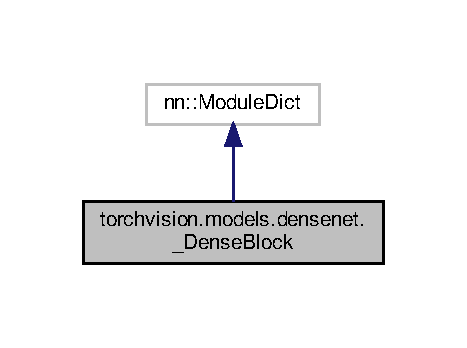
\includegraphics[width=224pt]{classtorchvision_1_1models_1_1densenet_1_1__DenseBlock__inherit__graph}
\end{center}
\end{figure}


Collaboration diagram for torchvision.\+models.\+densenet.\+\_\+\+Dense\+Block\+:
\nopagebreak
\begin{figure}[H]
\begin{center}
\leavevmode
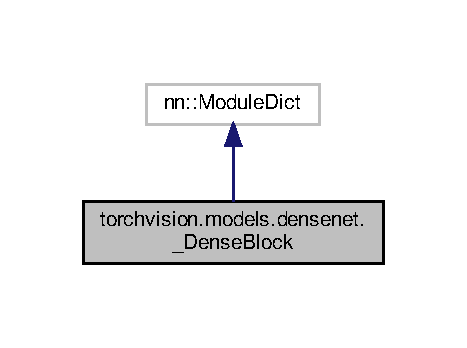
\includegraphics[width=224pt]{classtorchvision_1_1models_1_1densenet_1_1__DenseBlock__coll__graph}
\end{center}
\end{figure}
\subsection*{Public Member Functions}
\begin{DoxyCompactItemize}
\item 
\mbox{\Hypertarget{classtorchvision_1_1models_1_1densenet_1_1__DenseBlock_ab706187c8ead2ef16c70afc3586c64c2}\label{classtorchvision_1_1models_1_1densenet_1_1__DenseBlock_ab706187c8ead2ef16c70afc3586c64c2}} 
def {\bfseries \+\_\+\+\_\+init\+\_\+\+\_\+} (self, num\+\_\+layers, num\+\_\+input\+\_\+features, bn\+\_\+size, growth\+\_\+rate, drop\+\_\+rate, memory\+\_\+efficient=False)
\item 
\mbox{\Hypertarget{classtorchvision_1_1models_1_1densenet_1_1__DenseBlock_ab9d463a6490a89f9a6e2244609a64ab3}\label{classtorchvision_1_1models_1_1densenet_1_1__DenseBlock_ab9d463a6490a89f9a6e2244609a64ab3}} 
def {\bfseries forward} (self, init\+\_\+features)
\end{DoxyCompactItemize}


\subsection{Detailed Description}


Definition at line 93 of file densenet.\+py.



The documentation for this class was generated from the following file\+:\begin{DoxyCompactItemize}
\item 
/home/jose/ros\+\_\+ws/src/gr\+\_\+perception/gr\+\_\+ml/nb/vision/torchvision/models/densenet.\+py\end{DoxyCompactItemize}

\hypertarget{structvision_1_1models_1_1__DenseBlockImpl}{}\section{vision\+:\+:models\+:\+:\+\_\+\+Dense\+Block\+Impl Struct Reference}
\label{structvision_1_1models_1_1__DenseBlockImpl}\index{vision\+::models\+::\+\_\+\+Dense\+Block\+Impl@{vision\+::models\+::\+\_\+\+Dense\+Block\+Impl}}


Inheritance diagram for vision\+:\+:models\+:\+:\+\_\+\+Dense\+Block\+Impl\+:
\nopagebreak
\begin{figure}[H]
\begin{center}
\leavevmode
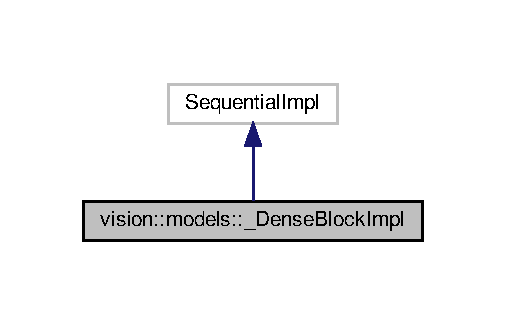
\includegraphics[width=243pt]{structvision_1_1models_1_1__DenseBlockImpl__inherit__graph}
\end{center}
\end{figure}


Collaboration diagram for vision\+:\+:models\+:\+:\+\_\+\+Dense\+Block\+Impl\+:
\nopagebreak
\begin{figure}[H]
\begin{center}
\leavevmode
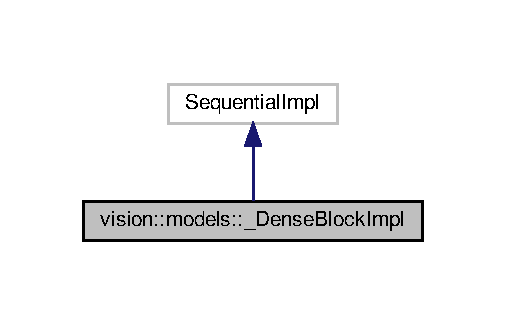
\includegraphics[width=243pt]{structvision_1_1models_1_1__DenseBlockImpl__coll__graph}
\end{center}
\end{figure}
\subsection*{Public Member Functions}
\begin{DoxyCompactItemize}
\item 
\mbox{\Hypertarget{structvision_1_1models_1_1__DenseBlockImpl_aaf609b5647834260f4b93da3bfbd387f}\label{structvision_1_1models_1_1__DenseBlockImpl_aaf609b5647834260f4b93da3bfbd387f}} 
{\bfseries \+\_\+\+Dense\+Block\+Impl} (int64\+\_\+t num\+\_\+layers, int64\+\_\+t num\+\_\+input\+\_\+features, int64\+\_\+t bn\+\_\+size, int64\+\_\+t growth\+\_\+rate, double drop\+\_\+rate)
\item 
\mbox{\Hypertarget{structvision_1_1models_1_1__DenseBlockImpl_a428f13647e411291d3f2c97b791dfe86}\label{structvision_1_1models_1_1__DenseBlockImpl_a428f13647e411291d3f2c97b791dfe86}} 
torch\+::\+Tensor {\bfseries forward} (torch\+::\+Tensor x)
\end{DoxyCompactItemize}


\subsection{Detailed Description}


Definition at line 46 of file densenet.\+cpp.



The documentation for this struct was generated from the following file\+:\begin{DoxyCompactItemize}
\item 
/home/jose/ros\+\_\+ws/src/gr\+\_\+perception/gr\+\_\+ml/nb/vision/torchvision/csrc/models/densenet.\+cpp\end{DoxyCompactItemize}

\hypertarget{classtorchvision_1_1models_1_1densenet_1_1__DenseLayer}{}\section{torchvision.\+models.\+densenet.\+\_\+\+Dense\+Layer Class Reference}
\label{classtorchvision_1_1models_1_1densenet_1_1__DenseLayer}\index{torchvision.\+models.\+densenet.\+\_\+\+Dense\+Layer@{torchvision.\+models.\+densenet.\+\_\+\+Dense\+Layer}}


Inheritance diagram for torchvision.\+models.\+densenet.\+\_\+\+Dense\+Layer\+:
\nopagebreak
\begin{figure}[H]
\begin{center}
\leavevmode
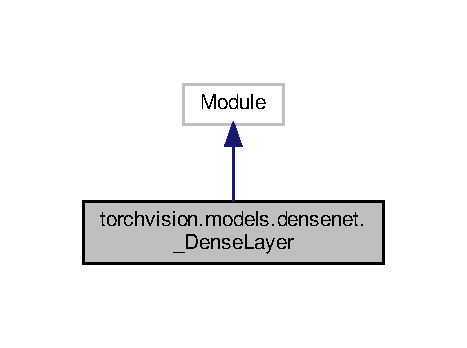
\includegraphics[width=224pt]{classtorchvision_1_1models_1_1densenet_1_1__DenseLayer__inherit__graph}
\end{center}
\end{figure}


Collaboration diagram for torchvision.\+models.\+densenet.\+\_\+\+Dense\+Layer\+:
\nopagebreak
\begin{figure}[H]
\begin{center}
\leavevmode
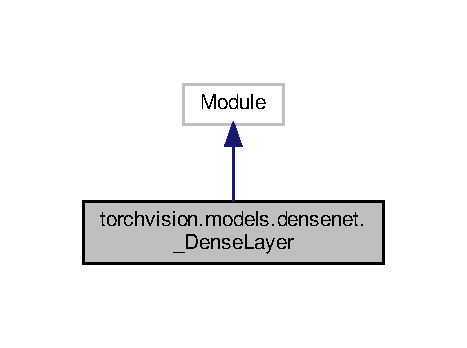
\includegraphics[width=224pt]{classtorchvision_1_1models_1_1densenet_1_1__DenseLayer__coll__graph}
\end{center}
\end{figure}
\subsection*{Public Member Functions}
\begin{DoxyCompactItemize}
\item 
\mbox{\Hypertarget{classtorchvision_1_1models_1_1densenet_1_1__DenseLayer_a9668043e6530dd3ff177721749ff5748}\label{classtorchvision_1_1models_1_1densenet_1_1__DenseLayer_a9668043e6530dd3ff177721749ff5748}} 
def {\bfseries \+\_\+\+\_\+init\+\_\+\+\_\+} (self, num\+\_\+input\+\_\+features, growth\+\_\+rate, bn\+\_\+size, drop\+\_\+rate, memory\+\_\+efficient=False)
\item 
\mbox{\Hypertarget{classtorchvision_1_1models_1_1densenet_1_1__DenseLayer_aab07069d4db2c9abe827f852e2fc9a9c}\label{classtorchvision_1_1models_1_1densenet_1_1__DenseLayer_aab07069d4db2c9abe827f852e2fc9a9c}} 
def {\bfseries bn\+\_\+function} (self, inputs)
\item 
\mbox{\Hypertarget{classtorchvision_1_1models_1_1densenet_1_1__DenseLayer_a5ac7859e83304930ce4e2333a0e4ab87}\label{classtorchvision_1_1models_1_1densenet_1_1__DenseLayer_a5ac7859e83304930ce4e2333a0e4ab87}} 
def {\bfseries any\+\_\+requires\+\_\+grad} (self, input)
\item 
\mbox{\Hypertarget{classtorchvision_1_1models_1_1densenet_1_1__DenseLayer_a69e6b580a2504dae3d3c2cf8f082d1b6}\label{classtorchvision_1_1models_1_1densenet_1_1__DenseLayer_a69e6b580a2504dae3d3c2cf8f082d1b6}} 
def {\bfseries call\+\_\+checkpoint\+\_\+bottleneck} (self, input)
\item 
\mbox{\Hypertarget{classtorchvision_1_1models_1_1densenet_1_1__DenseLayer_a1d07cf8bda875e365de5ef2f9ee911a2}\label{classtorchvision_1_1models_1_1densenet_1_1__DenseLayer_a1d07cf8bda875e365de5ef2f9ee911a2}} 
def {\bfseries forward} (self, input)
\item 
\mbox{\Hypertarget{classtorchvision_1_1models_1_1densenet_1_1__DenseLayer_a1d07cf8bda875e365de5ef2f9ee911a2}\label{classtorchvision_1_1models_1_1densenet_1_1__DenseLayer_a1d07cf8bda875e365de5ef2f9ee911a2}} 
def {\bfseries forward} (self, input)
\item 
\mbox{\Hypertarget{classtorchvision_1_1models_1_1densenet_1_1__DenseLayer_a1d07cf8bda875e365de5ef2f9ee911a2}\label{classtorchvision_1_1models_1_1densenet_1_1__DenseLayer_a1d07cf8bda875e365de5ef2f9ee911a2}} 
def {\bfseries forward} (self, input)
\end{DoxyCompactItemize}
\subsection*{Data Fields}
\begin{DoxyCompactItemize}
\item 
\mbox{\Hypertarget{classtorchvision_1_1models_1_1densenet_1_1__DenseLayer_a75a984035b2fbbea946b4537b5246d70}\label{classtorchvision_1_1models_1_1densenet_1_1__DenseLayer_a75a984035b2fbbea946b4537b5246d70}} 
{\bfseries drop\+\_\+rate}
\item 
\mbox{\Hypertarget{classtorchvision_1_1models_1_1densenet_1_1__DenseLayer_a6bd2268289a74a6250fe5b9d608446f7}\label{classtorchvision_1_1models_1_1densenet_1_1__DenseLayer_a6bd2268289a74a6250fe5b9d608446f7}} 
{\bfseries memory\+\_\+efficient}
\end{DoxyCompactItemize}


\subsection{Detailed Description}


Definition at line 22 of file densenet.\+py.



The documentation for this class was generated from the following file\+:\begin{DoxyCompactItemize}
\item 
/home/jose/ros\+\_\+ws/src/gr\+\_\+perception/gr\+\_\+ml/nb/vision/torchvision/models/densenet.\+py\end{DoxyCompactItemize}

\hypertarget{structvision_1_1models_1_1__DenseLayerImpl}{}\section{vision\+:\+:models\+:\+:\+\_\+\+Dense\+Layer\+Impl Struct Reference}
\label{structvision_1_1models_1_1__DenseLayerImpl}\index{vision\+::models\+::\+\_\+\+Dense\+Layer\+Impl@{vision\+::models\+::\+\_\+\+Dense\+Layer\+Impl}}


Inheritance diagram for vision\+:\+:models\+:\+:\+\_\+\+Dense\+Layer\+Impl\+:
\nopagebreak
\begin{figure}[H]
\begin{center}
\leavevmode
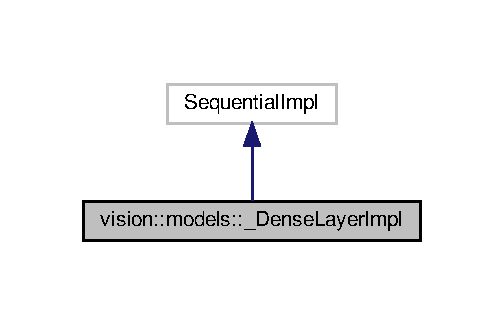
\includegraphics[width=242pt]{structvision_1_1models_1_1__DenseLayerImpl__inherit__graph}
\end{center}
\end{figure}


Collaboration diagram for vision\+:\+:models\+:\+:\+\_\+\+Dense\+Layer\+Impl\+:
\nopagebreak
\begin{figure}[H]
\begin{center}
\leavevmode
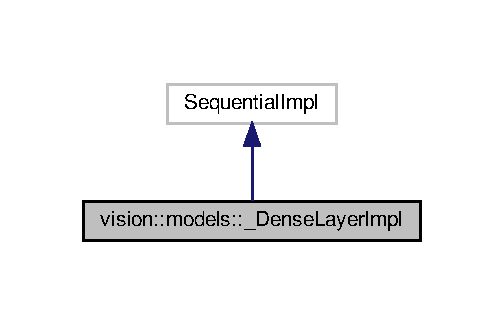
\includegraphics[width=242pt]{structvision_1_1models_1_1__DenseLayerImpl__coll__graph}
\end{center}
\end{figure}
\subsection*{Public Member Functions}
\begin{DoxyCompactItemize}
\item 
\mbox{\Hypertarget{structvision_1_1models_1_1__DenseLayerImpl_ae5f0f90dbc2c21de7b4dfeacd31bb678}\label{structvision_1_1models_1_1__DenseLayerImpl_ae5f0f90dbc2c21de7b4dfeacd31bb678}} 
{\bfseries \+\_\+\+Dense\+Layer\+Impl} (int64\+\_\+t num\+\_\+input\+\_\+features, int64\+\_\+t growth\+\_\+rate, int64\+\_\+t bn\+\_\+size, double drop\+\_\+rate)
\item 
\mbox{\Hypertarget{structvision_1_1models_1_1__DenseLayerImpl_a8aaef3408142548b005531756209aad4}\label{structvision_1_1models_1_1__DenseLayerImpl_a8aaef3408142548b005531756209aad4}} 
torch\+::\+Tensor {\bfseries forward} (torch\+::\+Tensor x)
\end{DoxyCompactItemize}
\subsection*{Data Fields}
\begin{DoxyCompactItemize}
\item 
\mbox{\Hypertarget{structvision_1_1models_1_1__DenseLayerImpl_a3fe117676f9b89df19f266bf77d0c713}\label{structvision_1_1models_1_1__DenseLayerImpl_a3fe117676f9b89df19f266bf77d0c713}} 
double {\bfseries drop\+\_\+rate}
\end{DoxyCompactItemize}


\subsection{Detailed Description}


Definition at line 9 of file densenet.\+cpp.



The documentation for this struct was generated from the following file\+:\begin{DoxyCompactItemize}
\item 
/home/jose/ros\+\_\+ws/src/gr\+\_\+perception/gr\+\_\+ml/nb/vision/torchvision/csrc/models/densenet.\+cpp\end{DoxyCompactItemize}

\hypertarget{classtorchvision_1_1models_1_1mnasnet_1_1__InvertedResidual}{}\section{torchvision.\+models.\+mnasnet.\+\_\+\+Inverted\+Residual Class Reference}
\label{classtorchvision_1_1models_1_1mnasnet_1_1__InvertedResidual}\index{torchvision.\+models.\+mnasnet.\+\_\+\+Inverted\+Residual@{torchvision.\+models.\+mnasnet.\+\_\+\+Inverted\+Residual}}


Inheritance diagram for torchvision.\+models.\+mnasnet.\+\_\+\+Inverted\+Residual\+:
\nopagebreak
\begin{figure}[H]
\begin{center}
\leavevmode
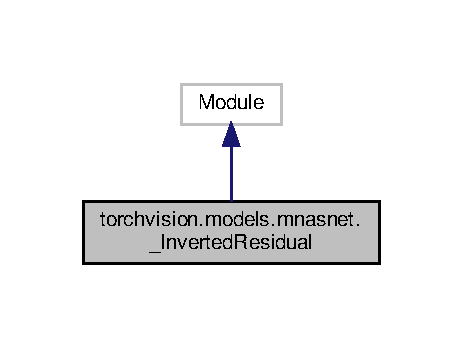
\includegraphics[width=222pt]{classtorchvision_1_1models_1_1mnasnet_1_1__InvertedResidual__inherit__graph}
\end{center}
\end{figure}


Collaboration diagram for torchvision.\+models.\+mnasnet.\+\_\+\+Inverted\+Residual\+:
\nopagebreak
\begin{figure}[H]
\begin{center}
\leavevmode
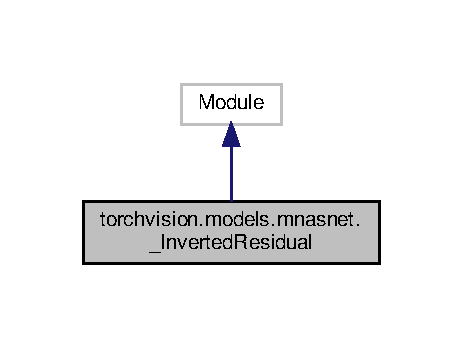
\includegraphics[width=222pt]{classtorchvision_1_1models_1_1mnasnet_1_1__InvertedResidual__coll__graph}
\end{center}
\end{figure}
\subsection*{Public Member Functions}
\begin{DoxyCompactItemize}
\item 
\mbox{\Hypertarget{classtorchvision_1_1models_1_1mnasnet_1_1__InvertedResidual_a1aaabc0732d8a5e09a82e92a2d8c1ce2}\label{classtorchvision_1_1models_1_1mnasnet_1_1__InvertedResidual_a1aaabc0732d8a5e09a82e92a2d8c1ce2}} 
def {\bfseries \+\_\+\+\_\+init\+\_\+\+\_\+} (self, in\+\_\+ch, out\+\_\+ch, kernel\+\_\+size, stride, expansion\+\_\+factor, bn\+\_\+momentum=0.\+1)
\item 
\mbox{\Hypertarget{classtorchvision_1_1models_1_1mnasnet_1_1__InvertedResidual_a7e935aea2f25a765bc82b609043f7f0e}\label{classtorchvision_1_1models_1_1mnasnet_1_1__InvertedResidual_a7e935aea2f25a765bc82b609043f7f0e}} 
def {\bfseries forward} (self, input)
\end{DoxyCompactItemize}
\subsection*{Data Fields}
\begin{DoxyCompactItemize}
\item 
\mbox{\Hypertarget{classtorchvision_1_1models_1_1mnasnet_1_1__InvertedResidual_a85b4b4e4515faa7ca3c201be3019bd1c}\label{classtorchvision_1_1models_1_1mnasnet_1_1__InvertedResidual_a85b4b4e4515faa7ca3c201be3019bd1c}} 
{\bfseries apply\+\_\+residual}
\item 
\mbox{\Hypertarget{classtorchvision_1_1models_1_1mnasnet_1_1__InvertedResidual_af691d4125fec58d155b90db42e13076e}\label{classtorchvision_1_1models_1_1mnasnet_1_1__InvertedResidual_af691d4125fec58d155b90db42e13076e}} 
{\bfseries layers}
\end{DoxyCompactItemize}


\subsection{Detailed Description}


Definition at line 23 of file mnasnet.\+py.



The documentation for this class was generated from the following file\+:\begin{DoxyCompactItemize}
\item 
/home/jose/ros\+\_\+ws/src/gr\+\_\+perception/gr\+\_\+ml/nb/vision/torchvision/models/mnasnet.\+py\end{DoxyCompactItemize}

\hypertarget{classtorchvision_1_1models_1_1segmentation_1_1__utils_1_1__SimpleSegmentationModel}{}\section{torchvision.\+models.\+segmentation.\+\_\+utils.\+\_\+\+Simple\+Segmentation\+Model Class Reference}
\label{classtorchvision_1_1models_1_1segmentation_1_1__utils_1_1__SimpleSegmentationModel}\index{torchvision.\+models.\+segmentation.\+\_\+utils.\+\_\+\+Simple\+Segmentation\+Model@{torchvision.\+models.\+segmentation.\+\_\+utils.\+\_\+\+Simple\+Segmentation\+Model}}


Inheritance diagram for torchvision.\+models.\+segmentation.\+\_\+utils.\+\_\+\+Simple\+Segmentation\+Model\+:
\nopagebreak
\begin{figure}[H]
\begin{center}
\leavevmode
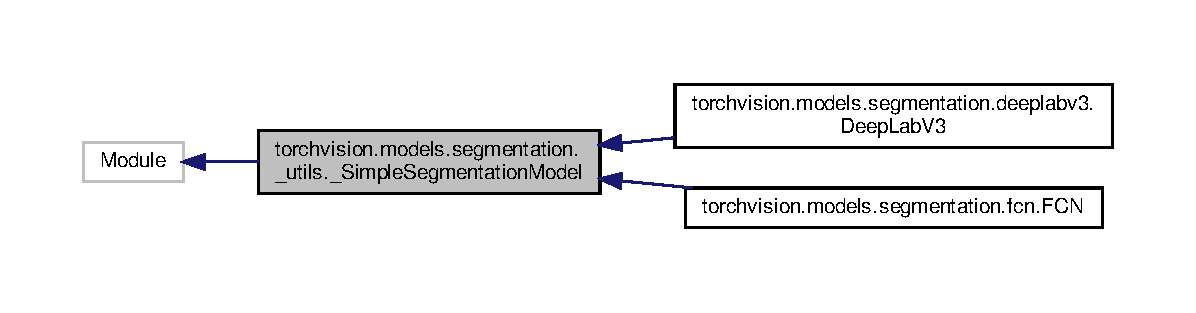
\includegraphics[width=350pt]{classtorchvision_1_1models_1_1segmentation_1_1__utils_1_1__SimpleSegmentationModel__inherit__graph}
\end{center}
\end{figure}


Collaboration diagram for torchvision.\+models.\+segmentation.\+\_\+utils.\+\_\+\+Simple\+Segmentation\+Model\+:
\nopagebreak
\begin{figure}[H]
\begin{center}
\leavevmode
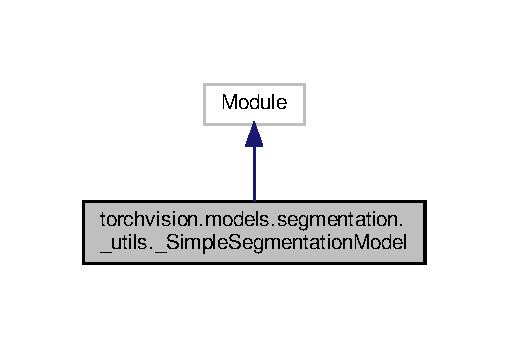
\includegraphics[width=244pt]{classtorchvision_1_1models_1_1segmentation_1_1__utils_1_1__SimpleSegmentationModel__coll__graph}
\end{center}
\end{figure}
\subsection*{Public Member Functions}
\begin{DoxyCompactItemize}
\item 
\mbox{\Hypertarget{classtorchvision_1_1models_1_1segmentation_1_1__utils_1_1__SimpleSegmentationModel_acaef16d1af756c53b98270674286ed67}\label{classtorchvision_1_1models_1_1segmentation_1_1__utils_1_1__SimpleSegmentationModel_acaef16d1af756c53b98270674286ed67}} 
def {\bfseries \+\_\+\+\_\+init\+\_\+\+\_\+} (self, backbone, classifier, aux\+\_\+classifier=None)
\item 
\mbox{\Hypertarget{classtorchvision_1_1models_1_1segmentation_1_1__utils_1_1__SimpleSegmentationModel_ad3f553dfa2f6f5e1acf1223ae0ead28c}\label{classtorchvision_1_1models_1_1segmentation_1_1__utils_1_1__SimpleSegmentationModel_ad3f553dfa2f6f5e1acf1223ae0ead28c}} 
def {\bfseries forward} (self, x)
\end{DoxyCompactItemize}
\subsection*{Data Fields}
\begin{DoxyCompactItemize}
\item 
\mbox{\Hypertarget{classtorchvision_1_1models_1_1segmentation_1_1__utils_1_1__SimpleSegmentationModel_a3c4fbe181befc38130cafaadad235b18}\label{classtorchvision_1_1models_1_1segmentation_1_1__utils_1_1__SimpleSegmentationModel_a3c4fbe181befc38130cafaadad235b18}} 
{\bfseries backbone}
\item 
\mbox{\Hypertarget{classtorchvision_1_1models_1_1segmentation_1_1__utils_1_1__SimpleSegmentationModel_aee7a264bd50c3f2714937f5a8633b2fd}\label{classtorchvision_1_1models_1_1segmentation_1_1__utils_1_1__SimpleSegmentationModel_aee7a264bd50c3f2714937f5a8633b2fd}} 
{\bfseries classifier}
\item 
\mbox{\Hypertarget{classtorchvision_1_1models_1_1segmentation_1_1__utils_1_1__SimpleSegmentationModel_a4b3d4afb07c52eafd29b28fd657c3efd}\label{classtorchvision_1_1models_1_1segmentation_1_1__utils_1_1__SimpleSegmentationModel_a4b3d4afb07c52eafd29b28fd657c3efd}} 
{\bfseries aux\+\_\+classifier}
\end{DoxyCompactItemize}


\subsection{Detailed Description}


Definition at line 8 of file \+\_\+utils.\+py.



The documentation for this class was generated from the following file\+:\begin{DoxyCompactItemize}
\item 
/home/jose/ros\+\_\+ws/src/gr\+\_\+perception/gr\+\_\+ml/nb/vision/torchvision/models/segmentation/\+\_\+utils.\+py\end{DoxyCompactItemize}

\hypertarget{classtorchvision_1_1models_1_1densenet_1_1__Transition}{}\section{torchvision.\+models.\+densenet.\+\_\+\+Transition Class Reference}
\label{classtorchvision_1_1models_1_1densenet_1_1__Transition}\index{torchvision.\+models.\+densenet.\+\_\+\+Transition@{torchvision.\+models.\+densenet.\+\_\+\+Transition}}


Inheritance diagram for torchvision.\+models.\+densenet.\+\_\+\+Transition\+:
\nopagebreak
\begin{figure}[H]
\begin{center}
\leavevmode
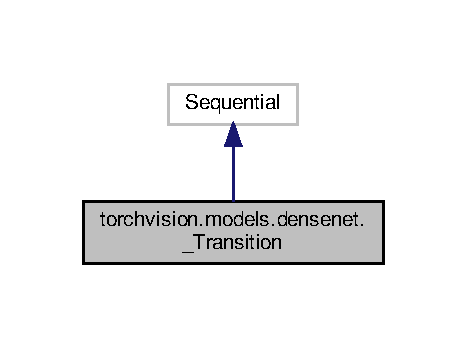
\includegraphics[width=224pt]{classtorchvision_1_1models_1_1densenet_1_1__Transition__inherit__graph}
\end{center}
\end{figure}


Collaboration diagram for torchvision.\+models.\+densenet.\+\_\+\+Transition\+:
\nopagebreak
\begin{figure}[H]
\begin{center}
\leavevmode
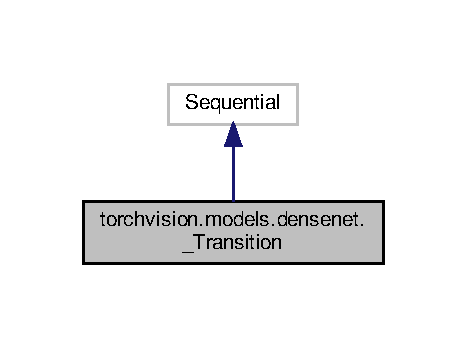
\includegraphics[width=224pt]{classtorchvision_1_1models_1_1densenet_1_1__Transition__coll__graph}
\end{center}
\end{figure}
\subsection*{Public Member Functions}
\begin{DoxyCompactItemize}
\item 
\mbox{\Hypertarget{classtorchvision_1_1models_1_1densenet_1_1__Transition_a697041fed7c1b0b40cbc47efd273eb14}\label{classtorchvision_1_1models_1_1densenet_1_1__Transition_a697041fed7c1b0b40cbc47efd273eb14}} 
def {\bfseries \+\_\+\+\_\+init\+\_\+\+\_\+} (self, num\+\_\+input\+\_\+features, num\+\_\+output\+\_\+features)
\end{DoxyCompactItemize}


\subsection{Detailed Description}


Definition at line 116 of file densenet.\+py.



The documentation for this class was generated from the following file\+:\begin{DoxyCompactItemize}
\item 
/home/jose/ros\+\_\+ws/src/gr\+\_\+perception/gr\+\_\+ml/nb/vision/torchvision/models/densenet.\+py\end{DoxyCompactItemize}

\hypertarget{structvision_1_1models_1_1__TransitionImpl}{}\section{vision\+:\+:models\+:\+:\+\_\+\+Transition\+Impl Struct Reference}
\label{structvision_1_1models_1_1__TransitionImpl}\index{vision\+::models\+::\+\_\+\+Transition\+Impl@{vision\+::models\+::\+\_\+\+Transition\+Impl}}


Inheritance diagram for vision\+:\+:models\+:\+:\+\_\+\+Transition\+Impl\+:
\nopagebreak
\begin{figure}[H]
\begin{center}
\leavevmode
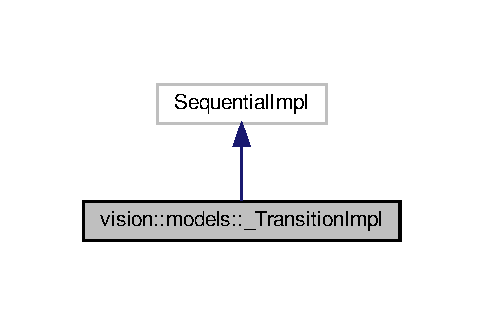
\includegraphics[width=232pt]{structvision_1_1models_1_1__TransitionImpl__inherit__graph}
\end{center}
\end{figure}


Collaboration diagram for vision\+:\+:models\+:\+:\+\_\+\+Transition\+Impl\+:
\nopagebreak
\begin{figure}[H]
\begin{center}
\leavevmode
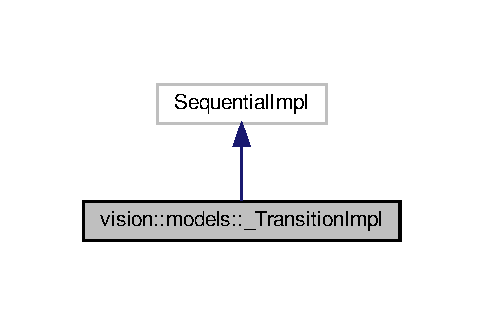
\includegraphics[width=232pt]{structvision_1_1models_1_1__TransitionImpl__coll__graph}
\end{center}
\end{figure}
\subsection*{Public Member Functions}
\begin{DoxyCompactItemize}
\item 
\mbox{\Hypertarget{structvision_1_1models_1_1__TransitionImpl_a2918f4faba969b1d9218adf3a4b7e35d}\label{structvision_1_1models_1_1__TransitionImpl_a2918f4faba969b1d9218adf3a4b7e35d}} 
{\bfseries \+\_\+\+Transition\+Impl} (int64\+\_\+t num\+\_\+input\+\_\+features, int64\+\_\+t num\+\_\+output\+\_\+features)
\item 
\mbox{\Hypertarget{structvision_1_1models_1_1__TransitionImpl_aef2707ad2d01751cd93cfc6e430b14b5}\label{structvision_1_1models_1_1__TransitionImpl_aef2707ad2d01751cd93cfc6e430b14b5}} 
torch\+::\+Tensor {\bfseries forward} (torch\+::\+Tensor x)
\end{DoxyCompactItemize}


\subsection{Detailed Description}


Definition at line 70 of file densenet.\+cpp.



The documentation for this struct was generated from the following file\+:\begin{DoxyCompactItemize}
\item 
/home/jose/ros\+\_\+ws/src/gr\+\_\+perception/gr\+\_\+ml/nb/vision/torchvision/csrc/models/densenet.\+cpp\end{DoxyCompactItemize}

\hypertarget{classtorchvision_1_1datasets_1_1video__utils_1_1__VideoTimestampsDataset}{}\section{torchvision.\+datasets.\+video\+\_\+utils.\+\_\+\+Video\+Timestamps\+Dataset Class Reference}
\label{classtorchvision_1_1datasets_1_1video__utils_1_1__VideoTimestampsDataset}\index{torchvision.\+datasets.\+video\+\_\+utils.\+\_\+\+Video\+Timestamps\+Dataset@{torchvision.\+datasets.\+video\+\_\+utils.\+\_\+\+Video\+Timestamps\+Dataset}}


Inheritance diagram for torchvision.\+datasets.\+video\+\_\+utils.\+\_\+\+Video\+Timestamps\+Dataset\+:
\nopagebreak
\begin{figure}[H]
\begin{center}
\leavevmode
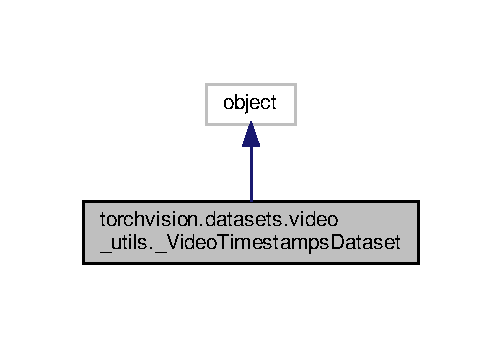
\includegraphics[width=241pt]{classtorchvision_1_1datasets_1_1video__utils_1_1__VideoTimestampsDataset__inherit__graph}
\end{center}
\end{figure}


Collaboration diagram for torchvision.\+datasets.\+video\+\_\+utils.\+\_\+\+Video\+Timestamps\+Dataset\+:
\nopagebreak
\begin{figure}[H]
\begin{center}
\leavevmode
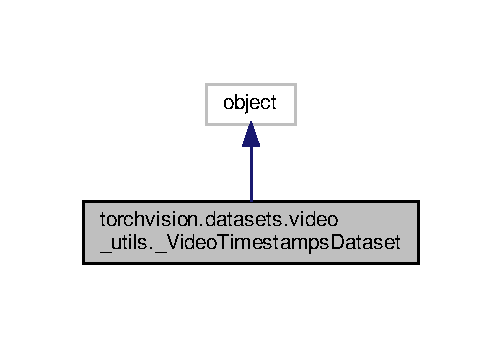
\includegraphics[width=241pt]{classtorchvision_1_1datasets_1_1video__utils_1_1__VideoTimestampsDataset__coll__graph}
\end{center}
\end{figure}
\subsection*{Public Member Functions}
\begin{DoxyCompactItemize}
\item 
\mbox{\Hypertarget{classtorchvision_1_1datasets_1_1video__utils_1_1__VideoTimestampsDataset_a19c146e81600b707068335da1e2931cb}\label{classtorchvision_1_1datasets_1_1video__utils_1_1__VideoTimestampsDataset_a19c146e81600b707068335da1e2931cb}} 
def {\bfseries \+\_\+\+\_\+init\+\_\+\+\_\+}
\item 
\mbox{\Hypertarget{classtorchvision_1_1datasets_1_1video__utils_1_1__VideoTimestampsDataset_af64c9729e5cb806988f971d46aee9d9c}\label{classtorchvision_1_1datasets_1_1video__utils_1_1__VideoTimestampsDataset_af64c9729e5cb806988f971d46aee9d9c}} 
def {\bfseries \+\_\+\+\_\+len\+\_\+\+\_\+} (self)
\item 
\mbox{\Hypertarget{classtorchvision_1_1datasets_1_1video__utils_1_1__VideoTimestampsDataset_a094e4540bf893da8e4003efd8f62a1f7}\label{classtorchvision_1_1datasets_1_1video__utils_1_1__VideoTimestampsDataset_a094e4540bf893da8e4003efd8f62a1f7}} 
def {\bfseries \+\_\+\+\_\+getitem\+\_\+\+\_\+} (self, idx)
\end{DoxyCompactItemize}
\subsection*{Data Fields}
\begin{DoxyCompactItemize}
\item 
\mbox{\Hypertarget{classtorchvision_1_1datasets_1_1video__utils_1_1__VideoTimestampsDataset_a840a98a4601de8bcdcf5def269306949}\label{classtorchvision_1_1datasets_1_1video__utils_1_1__VideoTimestampsDataset_a840a98a4601de8bcdcf5def269306949}} 
{\bfseries video\+\_\+paths}
\end{DoxyCompactItemize}


\subsection{Detailed Description}
\begin{DoxyVerb}Dataset used to parallelize the reading of the timestamps
of a list of videos, given their paths in the filesystem.

Used in VideoClips and defined at top level so it can be
pickled when forking.
\end{DoxyVerb}
 

Definition at line 49 of file video\+\_\+utils.\+py.



The documentation for this class was generated from the following file\+:\begin{DoxyCompactItemize}
\item 
/home/jose/ros\+\_\+ws/src/gr\+\_\+perception/gr\+\_\+ml/nb/vision/torchvision/datasets/video\+\_\+utils.\+py\end{DoxyCompactItemize}

\hypertarget{classutils_1_1transforms_1_1AbsoluteLabels}{}\section{utils.\+transforms.\+Absolute\+Labels Class Reference}
\label{classutils_1_1transforms_1_1AbsoluteLabels}\index{utils.\+transforms.\+Absolute\+Labels@{utils.\+transforms.\+Absolute\+Labels}}


Inheritance diagram for utils.\+transforms.\+Absolute\+Labels\+:
\nopagebreak
\begin{figure}[H]
\begin{center}
\leavevmode
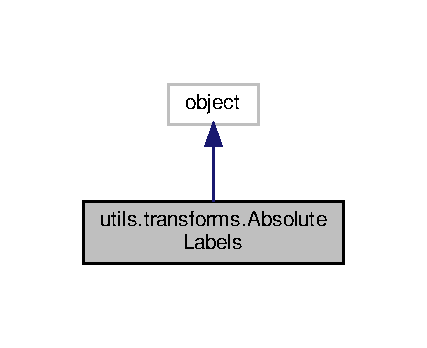
\includegraphics[width=205pt]{classutils_1_1transforms_1_1AbsoluteLabels__inherit__graph}
\end{center}
\end{figure}


Collaboration diagram for utils.\+transforms.\+Absolute\+Labels\+:
\nopagebreak
\begin{figure}[H]
\begin{center}
\leavevmode
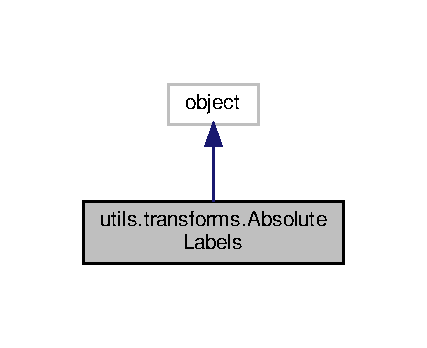
\includegraphics[width=205pt]{classutils_1_1transforms_1_1AbsoluteLabels__coll__graph}
\end{center}
\end{figure}
\subsection*{Public Member Functions}
\begin{DoxyCompactItemize}
\item 
\mbox{\Hypertarget{classutils_1_1transforms_1_1AbsoluteLabels_ac5bfffda1c3f3c8626fd83ba8fd4acb4}\label{classutils_1_1transforms_1_1AbsoluteLabels_ac5bfffda1c3f3c8626fd83ba8fd4acb4}} 
def {\bfseries \+\_\+\+\_\+init\+\_\+\+\_\+} (self)
\item 
\mbox{\Hypertarget{classutils_1_1transforms_1_1AbsoluteLabels_aeb4efe3914e346b8116d167188ed3f17}\label{classutils_1_1transforms_1_1AbsoluteLabels_aeb4efe3914e346b8116d167188ed3f17}} 
def {\bfseries \+\_\+\+\_\+call\+\_\+\+\_\+} (self, data)
\end{DoxyCompactItemize}


\subsection{Detailed Description}


Definition at line 69 of file transforms.\+py.



The documentation for this class was generated from the following file\+:\begin{DoxyCompactItemize}
\item 
/home/jose/ros\+\_\+ws/src/gr\+\_\+perception/gr\+\_\+ml/nb/yolov3/utils/transforms.\+py\end{DoxyCompactItemize}

\hypertarget{classtorchvision_1_1models_1_1alexnet_1_1AlexNet}{}\section{torchvision.\+models.\+alexnet.\+Alex\+Net Class Reference}
\label{classtorchvision_1_1models_1_1alexnet_1_1AlexNet}\index{torchvision.\+models.\+alexnet.\+Alex\+Net@{torchvision.\+models.\+alexnet.\+Alex\+Net}}


Inheritance diagram for torchvision.\+models.\+alexnet.\+Alex\+Net\+:
\nopagebreak
\begin{figure}[H]
\begin{center}
\leavevmode
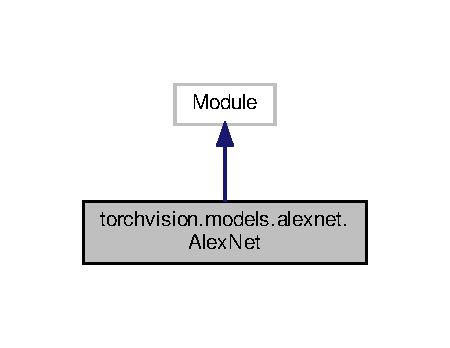
\includegraphics[width=216pt]{classtorchvision_1_1models_1_1alexnet_1_1AlexNet__inherit__graph}
\end{center}
\end{figure}


Collaboration diagram for torchvision.\+models.\+alexnet.\+Alex\+Net\+:
\nopagebreak
\begin{figure}[H]
\begin{center}
\leavevmode
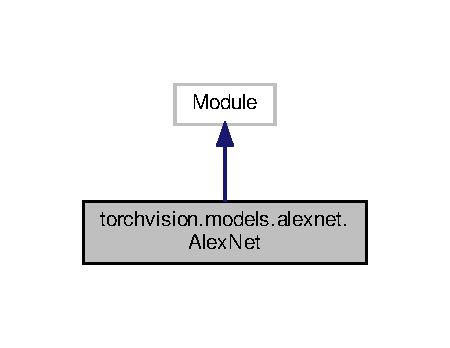
\includegraphics[width=216pt]{classtorchvision_1_1models_1_1alexnet_1_1AlexNet__coll__graph}
\end{center}
\end{figure}
\subsection*{Public Member Functions}
\begin{DoxyCompactItemize}
\item 
\mbox{\Hypertarget{classtorchvision_1_1models_1_1alexnet_1_1AlexNet_a586924af0af22619fdaae02fcb3e0d70}\label{classtorchvision_1_1models_1_1alexnet_1_1AlexNet_a586924af0af22619fdaae02fcb3e0d70}} 
def {\bfseries \+\_\+\+\_\+init\+\_\+\+\_\+} (self, num\+\_\+classes=1000)
\item 
\mbox{\Hypertarget{classtorchvision_1_1models_1_1alexnet_1_1AlexNet_a5355139784eee4ed268517b64c412eba}\label{classtorchvision_1_1models_1_1alexnet_1_1AlexNet_a5355139784eee4ed268517b64c412eba}} 
def {\bfseries forward} (self, x)
\end{DoxyCompactItemize}
\subsection*{Data Fields}
\begin{DoxyCompactItemize}
\item 
\mbox{\Hypertarget{classtorchvision_1_1models_1_1alexnet_1_1AlexNet_a294f8087de77e22d6c50321fcafb2e0e}\label{classtorchvision_1_1models_1_1alexnet_1_1AlexNet_a294f8087de77e22d6c50321fcafb2e0e}} 
{\bfseries features}
\item 
\mbox{\Hypertarget{classtorchvision_1_1models_1_1alexnet_1_1AlexNet_aa534d5eaae3a277bfb265c4a78cfbc04}\label{classtorchvision_1_1models_1_1alexnet_1_1AlexNet_aa534d5eaae3a277bfb265c4a78cfbc04}} 
{\bfseries avgpool}
\item 
\mbox{\Hypertarget{classtorchvision_1_1models_1_1alexnet_1_1AlexNet_a852beea893bee8b8ace771e6ede0d5ef}\label{classtorchvision_1_1models_1_1alexnet_1_1AlexNet_a852beea893bee8b8ace771e6ede0d5ef}} 
{\bfseries classifier}
\end{DoxyCompactItemize}


\subsection{Detailed Description}


Definition at line 14 of file alexnet.\+py.



The documentation for this class was generated from the following file\+:\begin{DoxyCompactItemize}
\item 
/home/jose/ros\+\_\+ws/src/gr\+\_\+perception/gr\+\_\+ml/nb/vision/torchvision/models/alexnet.\+py\end{DoxyCompactItemize}

\hypertarget{structvision_1_1models_1_1AlexNetImpl}{}\section{vision\+:\+:models\+:\+:Alex\+Net\+Impl Struct Reference}
\label{structvision_1_1models_1_1AlexNetImpl}\index{vision\+::models\+::\+Alex\+Net\+Impl@{vision\+::models\+::\+Alex\+Net\+Impl}}


Inheritance diagram for vision\+:\+:models\+:\+:Alex\+Net\+Impl\+:
\nopagebreak
\begin{figure}[H]
\begin{center}
\leavevmode
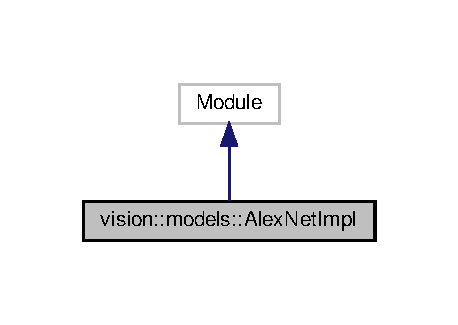
\includegraphics[width=220pt]{structvision_1_1models_1_1AlexNetImpl__inherit__graph}
\end{center}
\end{figure}


Collaboration diagram for vision\+:\+:models\+:\+:Alex\+Net\+Impl\+:
\nopagebreak
\begin{figure}[H]
\begin{center}
\leavevmode
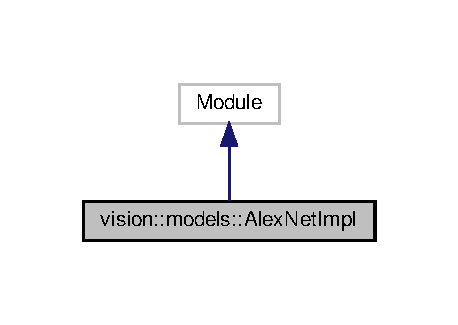
\includegraphics[width=220pt]{structvision_1_1models_1_1AlexNetImpl__coll__graph}
\end{center}
\end{figure}
\subsection*{Public Member Functions}
\begin{DoxyCompactItemize}
\item 
\mbox{\Hypertarget{structvision_1_1models_1_1AlexNetImpl_a61551564e4299747cd7ab7ac7d86e450}\label{structvision_1_1models_1_1AlexNetImpl_a61551564e4299747cd7ab7ac7d86e450}} 
{\bfseries Alex\+Net\+Impl} (int64\+\_\+t num\+\_\+classes=1000)
\item 
\mbox{\Hypertarget{structvision_1_1models_1_1AlexNetImpl_abcbd9a355fa73a53132ac39109aad671}\label{structvision_1_1models_1_1AlexNetImpl_abcbd9a355fa73a53132ac39109aad671}} 
torch\+::\+Tensor {\bfseries forward} (torch\+::\+Tensor x)
\end{DoxyCompactItemize}
\subsection*{Data Fields}
\begin{DoxyCompactItemize}
\item 
\mbox{\Hypertarget{structvision_1_1models_1_1AlexNetImpl_ab2534960e6a6c7bbd106a839240dd115}\label{structvision_1_1models_1_1AlexNetImpl_ab2534960e6a6c7bbd106a839240dd115}} 
torch\+::nn\+::\+Sequential {\bfseries features} \{nullptr\}
\item 
\mbox{\Hypertarget{structvision_1_1models_1_1AlexNetImpl_a5c2bbb6aaba8032c3567b020e2448a17}\label{structvision_1_1models_1_1AlexNetImpl_a5c2bbb6aaba8032c3567b020e2448a17}} 
torch\+::nn\+::\+Sequential {\bfseries classifier} \{nullptr\}
\end{DoxyCompactItemize}


\subsection{Detailed Description}


Definition at line 11 of file alexnet.\+h.



The documentation for this struct was generated from the following files\+:\begin{DoxyCompactItemize}
\item 
/home/jose/ros\+\_\+ws/src/gr\+\_\+perception/gr\+\_\+ml/nb/vision/torchvision/csrc/models/alexnet.\+h\item 
/home/jose/ros\+\_\+ws/src/gr\+\_\+perception/gr\+\_\+ml/nb/vision/torchvision/csrc/models/alexnet.\+cpp\end{DoxyCompactItemize}

\hypertarget{classtorchvision_1_1models_1_1detection_1_1rpn_1_1AnchorGenerator}{}\section{torchvision.\+models.\+detection.\+rpn.\+Anchor\+Generator Class Reference}
\label{classtorchvision_1_1models_1_1detection_1_1rpn_1_1AnchorGenerator}\index{torchvision.\+models.\+detection.\+rpn.\+Anchor\+Generator@{torchvision.\+models.\+detection.\+rpn.\+Anchor\+Generator}}


Inheritance diagram for torchvision.\+models.\+detection.\+rpn.\+Anchor\+Generator\+:
\nopagebreak
\begin{figure}[H]
\begin{center}
\leavevmode
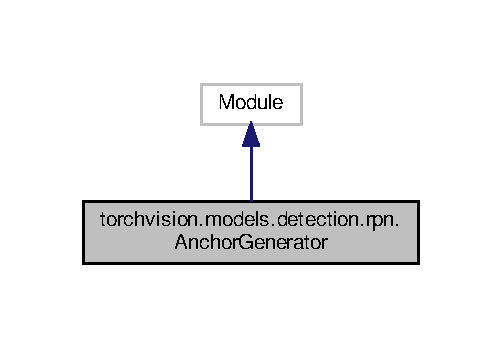
\includegraphics[width=241pt]{classtorchvision_1_1models_1_1detection_1_1rpn_1_1AnchorGenerator__inherit__graph}
\end{center}
\end{figure}


Collaboration diagram for torchvision.\+models.\+detection.\+rpn.\+Anchor\+Generator\+:
\nopagebreak
\begin{figure}[H]
\begin{center}
\leavevmode
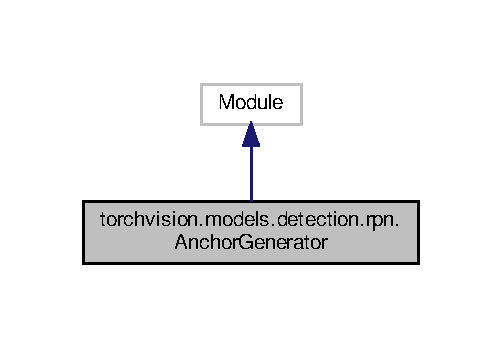
\includegraphics[width=241pt]{classtorchvision_1_1models_1_1detection_1_1rpn_1_1AnchorGenerator__coll__graph}
\end{center}
\end{figure}
\subsection*{Public Member Functions}
\begin{DoxyCompactItemize}
\item 
\mbox{\Hypertarget{classtorchvision_1_1models_1_1detection_1_1rpn_1_1AnchorGenerator_a4edc8d7050587f1b47e7e9a0bb9d7129}\label{classtorchvision_1_1models_1_1detection_1_1rpn_1_1AnchorGenerator_a4edc8d7050587f1b47e7e9a0bb9d7129}} 
def {\bfseries \+\_\+\+\_\+init\+\_\+\+\_\+} (self, sizes=(128, 256, 512), aspect\+\_\+ratios=(0.\+5, 1.\+0, 2.\+0))
\item 
\mbox{\Hypertarget{classtorchvision_1_1models_1_1detection_1_1rpn_1_1AnchorGenerator_a0d018ec8e2576e282a915cdee14aa3db}\label{classtorchvision_1_1models_1_1detection_1_1rpn_1_1AnchorGenerator_a0d018ec8e2576e282a915cdee14aa3db}} 
def {\bfseries generate\+\_\+anchors} (self, scales, aspect\+\_\+ratios, dtype=torch.\+float32, device=\char`\"{}cpu\char`\"{})
\item 
\mbox{\Hypertarget{classtorchvision_1_1models_1_1detection_1_1rpn_1_1AnchorGenerator_aea54ce6f6d80e2615d6a98e2d27771a7}\label{classtorchvision_1_1models_1_1detection_1_1rpn_1_1AnchorGenerator_aea54ce6f6d80e2615d6a98e2d27771a7}} 
def {\bfseries set\+\_\+cell\+\_\+anchors} (self, dtype, device)
\item 
\mbox{\Hypertarget{classtorchvision_1_1models_1_1detection_1_1rpn_1_1AnchorGenerator_a9b1c33a3e35015cd653c31f4db62c697}\label{classtorchvision_1_1models_1_1detection_1_1rpn_1_1AnchorGenerator_a9b1c33a3e35015cd653c31f4db62c697}} 
def {\bfseries num\+\_\+anchors\+\_\+per\+\_\+location} (self)
\item 
\mbox{\Hypertarget{classtorchvision_1_1models_1_1detection_1_1rpn_1_1AnchorGenerator_a12b4dba4ceb199ad95af5eee939a0251}\label{classtorchvision_1_1models_1_1detection_1_1rpn_1_1AnchorGenerator_a12b4dba4ceb199ad95af5eee939a0251}} 
def {\bfseries grid\+\_\+anchors} (self, grid\+\_\+sizes, strides)
\item 
\mbox{\Hypertarget{classtorchvision_1_1models_1_1detection_1_1rpn_1_1AnchorGenerator_a8b50db7adcf16fd4b05c90358d6aeaa7}\label{classtorchvision_1_1models_1_1detection_1_1rpn_1_1AnchorGenerator_a8b50db7adcf16fd4b05c90358d6aeaa7}} 
def {\bfseries cached\+\_\+grid\+\_\+anchors} (self, grid\+\_\+sizes, strides)
\item 
\mbox{\Hypertarget{classtorchvision_1_1models_1_1detection_1_1rpn_1_1AnchorGenerator_ab5b24936f575ccfa5175663def4e3e86}\label{classtorchvision_1_1models_1_1detection_1_1rpn_1_1AnchorGenerator_ab5b24936f575ccfa5175663def4e3e86}} 
def {\bfseries forward} (self, image\+\_\+list, feature\+\_\+maps)
\end{DoxyCompactItemize}
\subsection*{Data Fields}
\begin{DoxyCompactItemize}
\item 
\mbox{\Hypertarget{classtorchvision_1_1models_1_1detection_1_1rpn_1_1AnchorGenerator_afd8b8d1bb3aaae5fa592df4dc5178451}\label{classtorchvision_1_1models_1_1detection_1_1rpn_1_1AnchorGenerator_afd8b8d1bb3aaae5fa592df4dc5178451}} 
{\bfseries sizes}
\item 
\mbox{\Hypertarget{classtorchvision_1_1models_1_1detection_1_1rpn_1_1AnchorGenerator_ac02bffc42b572cc938d3fcff0d9bde7e}\label{classtorchvision_1_1models_1_1detection_1_1rpn_1_1AnchorGenerator_ac02bffc42b572cc938d3fcff0d9bde7e}} 
{\bfseries aspect\+\_\+ratios}
\item 
\mbox{\Hypertarget{classtorchvision_1_1models_1_1detection_1_1rpn_1_1AnchorGenerator_a10f0af36916c276ae4c1ddac2b499548}\label{classtorchvision_1_1models_1_1detection_1_1rpn_1_1AnchorGenerator_a10f0af36916c276ae4c1ddac2b499548}} 
{\bfseries cell\+\_\+anchors}
\end{DoxyCompactItemize}


\subsection{Detailed Description}


Definition at line 27 of file rpn.\+py.



The documentation for this class was generated from the following file\+:\begin{DoxyCompactItemize}
\item 
/home/jose/ros\+\_\+ws/src/gr\+\_\+perception/gr\+\_\+ml/nb/vision/torchvision/models/detection/rpn.\+py\end{DoxyCompactItemize}

\hypertarget{classtorchvision_1_1models_1_1segmentation_1_1deeplabv3_1_1ASPP}{}\section{torchvision.\+models.\+segmentation.\+deeplabv3.\+A\+S\+PP Class Reference}
\label{classtorchvision_1_1models_1_1segmentation_1_1deeplabv3_1_1ASPP}\index{torchvision.\+models.\+segmentation.\+deeplabv3.\+A\+S\+PP@{torchvision.\+models.\+segmentation.\+deeplabv3.\+A\+S\+PP}}


Inheritance diagram for torchvision.\+models.\+segmentation.\+deeplabv3.\+A\+S\+PP\+:
\nopagebreak
\begin{figure}[H]
\begin{center}
\leavevmode
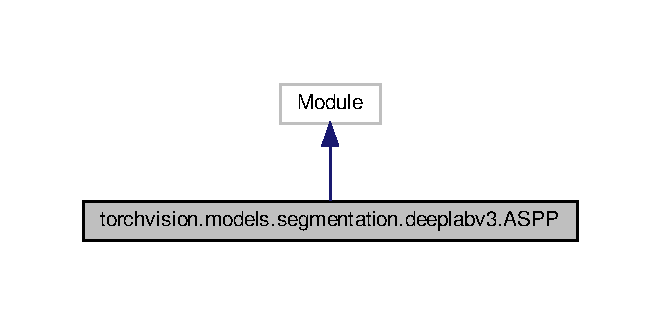
\includegraphics[width=317pt]{classtorchvision_1_1models_1_1segmentation_1_1deeplabv3_1_1ASPP__inherit__graph}
\end{center}
\end{figure}


Collaboration diagram for torchvision.\+models.\+segmentation.\+deeplabv3.\+A\+S\+PP\+:
\nopagebreak
\begin{figure}[H]
\begin{center}
\leavevmode
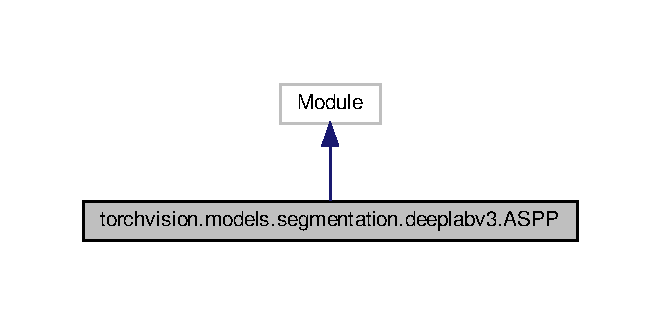
\includegraphics[width=317pt]{classtorchvision_1_1models_1_1segmentation_1_1deeplabv3_1_1ASPP__coll__graph}
\end{center}
\end{figure}
\subsection*{Public Member Functions}
\begin{DoxyCompactItemize}
\item 
\mbox{\Hypertarget{classtorchvision_1_1models_1_1segmentation_1_1deeplabv3_1_1ASPP_aac480fc9b934b64c94087ff9607b66b9}\label{classtorchvision_1_1models_1_1segmentation_1_1deeplabv3_1_1ASPP_aac480fc9b934b64c94087ff9607b66b9}} 
def {\bfseries \+\_\+\+\_\+init\+\_\+\+\_\+} (self, in\+\_\+channels, atrous\+\_\+rates, out\+\_\+channels=256)
\item 
\mbox{\Hypertarget{classtorchvision_1_1models_1_1segmentation_1_1deeplabv3_1_1ASPP_a7579b0ff151fc4b1b25aa3a55acc8f25}\label{classtorchvision_1_1models_1_1segmentation_1_1deeplabv3_1_1ASPP_a7579b0ff151fc4b1b25aa3a55acc8f25}} 
def {\bfseries forward} (self, x)
\end{DoxyCompactItemize}
\subsection*{Data Fields}
\begin{DoxyCompactItemize}
\item 
\mbox{\Hypertarget{classtorchvision_1_1models_1_1segmentation_1_1deeplabv3_1_1ASPP_a9857bb28022bb8f5687b6400c0a1ea65}\label{classtorchvision_1_1models_1_1segmentation_1_1deeplabv3_1_1ASPP_a9857bb28022bb8f5687b6400c0a1ea65}} 
{\bfseries convs}
\item 
\mbox{\Hypertarget{classtorchvision_1_1models_1_1segmentation_1_1deeplabv3_1_1ASPP_ab020c2e0fbbf79e9b4d2c9cc1ee1189b}\label{classtorchvision_1_1models_1_1segmentation_1_1deeplabv3_1_1ASPP_ab020c2e0fbbf79e9b4d2c9cc1ee1189b}} 
{\bfseries project}
\end{DoxyCompactItemize}


\subsection{Detailed Description}


Definition at line 65 of file deeplabv3.\+py.



The documentation for this class was generated from the following file\+:\begin{DoxyCompactItemize}
\item 
/home/jose/ros\+\_\+ws/src/gr\+\_\+perception/gr\+\_\+ml/nb/vision/torchvision/models/segmentation/deeplabv3.\+py\end{DoxyCompactItemize}

\hypertarget{classtorchvision_1_1models_1_1segmentation_1_1deeplabv3_1_1ASPPConv}{}\section{torchvision.\+models.\+segmentation.\+deeplabv3.\+A\+S\+P\+P\+Conv Class Reference}
\label{classtorchvision_1_1models_1_1segmentation_1_1deeplabv3_1_1ASPPConv}\index{torchvision.\+models.\+segmentation.\+deeplabv3.\+A\+S\+P\+P\+Conv@{torchvision.\+models.\+segmentation.\+deeplabv3.\+A\+S\+P\+P\+Conv}}


Inheritance diagram for torchvision.\+models.\+segmentation.\+deeplabv3.\+A\+S\+P\+P\+Conv\+:
\nopagebreak
\begin{figure}[H]
\begin{center}
\leavevmode
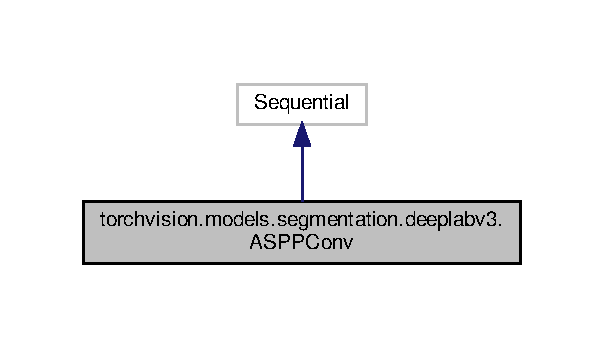
\includegraphics[width=290pt]{classtorchvision_1_1models_1_1segmentation_1_1deeplabv3_1_1ASPPConv__inherit__graph}
\end{center}
\end{figure}


Collaboration diagram for torchvision.\+models.\+segmentation.\+deeplabv3.\+A\+S\+P\+P\+Conv\+:
\nopagebreak
\begin{figure}[H]
\begin{center}
\leavevmode
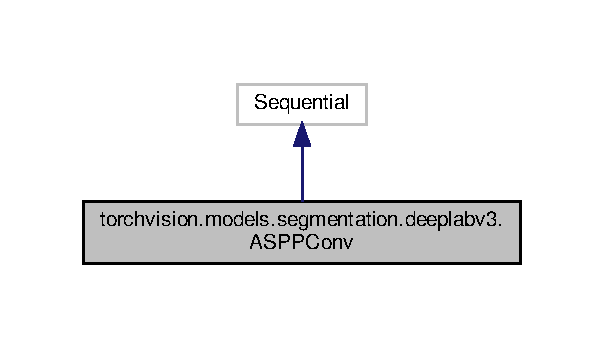
\includegraphics[width=290pt]{classtorchvision_1_1models_1_1segmentation_1_1deeplabv3_1_1ASPPConv__coll__graph}
\end{center}
\end{figure}
\subsection*{Public Member Functions}
\begin{DoxyCompactItemize}
\item 
\mbox{\Hypertarget{classtorchvision_1_1models_1_1segmentation_1_1deeplabv3_1_1ASPPConv_a7b45b9fca8ecd00cc2243417a49467e8}\label{classtorchvision_1_1models_1_1segmentation_1_1deeplabv3_1_1ASPPConv_a7b45b9fca8ecd00cc2243417a49467e8}} 
def {\bfseries \+\_\+\+\_\+init\+\_\+\+\_\+} (self, in\+\_\+channels, out\+\_\+channels, dilation)
\end{DoxyCompactItemize}


\subsection{Detailed Description}


Definition at line 40 of file deeplabv3.\+py.



The documentation for this class was generated from the following file\+:\begin{DoxyCompactItemize}
\item 
/home/jose/ros\+\_\+ws/src/gr\+\_\+perception/gr\+\_\+ml/nb/vision/torchvision/models/segmentation/deeplabv3.\+py\end{DoxyCompactItemize}

\hypertarget{classtorchvision_1_1models_1_1segmentation_1_1deeplabv3_1_1ASPPPooling}{}\section{torchvision.\+models.\+segmentation.\+deeplabv3.\+A\+S\+P\+P\+Pooling Class Reference}
\label{classtorchvision_1_1models_1_1segmentation_1_1deeplabv3_1_1ASPPPooling}\index{torchvision.\+models.\+segmentation.\+deeplabv3.\+A\+S\+P\+P\+Pooling@{torchvision.\+models.\+segmentation.\+deeplabv3.\+A\+S\+P\+P\+Pooling}}


Inheritance diagram for torchvision.\+models.\+segmentation.\+deeplabv3.\+A\+S\+P\+P\+Pooling\+:
\nopagebreak
\begin{figure}[H]
\begin{center}
\leavevmode
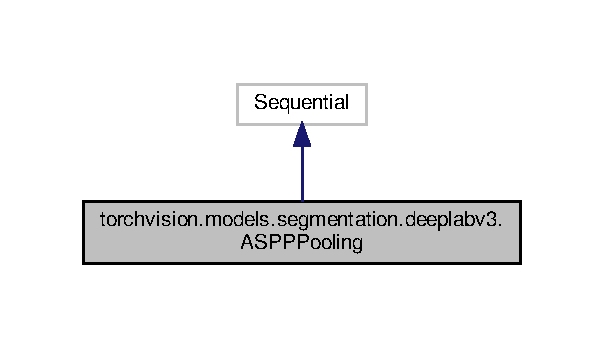
\includegraphics[width=290pt]{classtorchvision_1_1models_1_1segmentation_1_1deeplabv3_1_1ASPPPooling__inherit__graph}
\end{center}
\end{figure}


Collaboration diagram for torchvision.\+models.\+segmentation.\+deeplabv3.\+A\+S\+P\+P\+Pooling\+:
\nopagebreak
\begin{figure}[H]
\begin{center}
\leavevmode
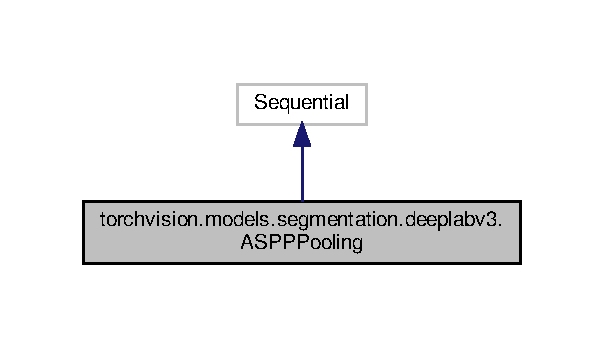
\includegraphics[width=290pt]{classtorchvision_1_1models_1_1segmentation_1_1deeplabv3_1_1ASPPPooling__coll__graph}
\end{center}
\end{figure}
\subsection*{Public Member Functions}
\begin{DoxyCompactItemize}
\item 
\mbox{\Hypertarget{classtorchvision_1_1models_1_1segmentation_1_1deeplabv3_1_1ASPPPooling_add161986b22a058aee93d1ebce97a83c}\label{classtorchvision_1_1models_1_1segmentation_1_1deeplabv3_1_1ASPPPooling_add161986b22a058aee93d1ebce97a83c}} 
def {\bfseries \+\_\+\+\_\+init\+\_\+\+\_\+} (self, in\+\_\+channels, out\+\_\+channels)
\item 
\mbox{\Hypertarget{classtorchvision_1_1models_1_1segmentation_1_1deeplabv3_1_1ASPPPooling_a16afde11dfcaa0aa09979e2bee6ba1e0}\label{classtorchvision_1_1models_1_1segmentation_1_1deeplabv3_1_1ASPPPooling_a16afde11dfcaa0aa09979e2bee6ba1e0}} 
def {\bfseries forward} (self, x)
\end{DoxyCompactItemize}


\subsection{Detailed Description}


Definition at line 50 of file deeplabv3.\+py.



The documentation for this class was generated from the following file\+:\begin{DoxyCompactItemize}
\item 
/home/jose/ros\+\_\+ws/src/gr\+\_\+perception/gr\+\_\+ml/nb/vision/torchvision/models/segmentation/deeplabv3.\+py\end{DoxyCompactItemize}

\hypertarget{structffmpeg_1_1AudioFormat}{}\section{ffmpeg\+:\+:Audio\+Format Struct Reference}
\label{structffmpeg_1_1AudioFormat}\index{ffmpeg\+::\+Audio\+Format@{ffmpeg\+::\+Audio\+Format}}
\subsection*{Public Member Functions}
\begin{DoxyCompactItemize}
\item 
\mbox{\Hypertarget{structffmpeg_1_1AudioFormat_ab2a29cb33630a31361b8ad993a3a0308}\label{structffmpeg_1_1AudioFormat_ab2a29cb33630a31361b8ad993a3a0308}} 
bool {\bfseries operator==} (const \hyperlink{structffmpeg_1_1AudioFormat}{Audio\+Format} \&x) const
\end{DoxyCompactItemize}
\subsection*{Data Fields}
\begin{DoxyCompactItemize}
\item 
\mbox{\Hypertarget{structffmpeg_1_1AudioFormat_a8a3b13bebf907c4ebfc119f82b8167ff}\label{structffmpeg_1_1AudioFormat_a8a3b13bebf907c4ebfc119f82b8167ff}} 
size\+\_\+t {\bfseries samples} \{0\}
\item 
\mbox{\Hypertarget{structffmpeg_1_1AudioFormat_a9fc06759ce4015167977216ef689fb87}\label{structffmpeg_1_1AudioFormat_a9fc06759ce4015167977216ef689fb87}} 
size\+\_\+t {\bfseries channels} \{0\}
\item 
\mbox{\Hypertarget{structffmpeg_1_1AudioFormat_a960b5692b622eabfbf29bb531456e084}\label{structffmpeg_1_1AudioFormat_a960b5692b622eabfbf29bb531456e084}} 
long {\bfseries format} \{-\/1\}
\item 
\mbox{\Hypertarget{structffmpeg_1_1AudioFormat_aff81802d03d3c936f68dde50c35464d9}\label{structffmpeg_1_1AudioFormat_aff81802d03d3c936f68dde50c35464d9}} 
size\+\_\+t {\bfseries padding} \mbox{[}2\mbox{]}
\end{DoxyCompactItemize}


\subsection{Detailed Description}


Definition at line 32 of file defs.\+h.



The documentation for this struct was generated from the following file\+:\begin{DoxyCompactItemize}
\item 
/home/jose/ros\+\_\+ws/src/gr\+\_\+perception/gr\+\_\+ml/nb/vision/torchvision/csrc/cpu/decoder/defs.\+h\end{DoxyCompactItemize}

\hypertarget{classffmpeg_1_1AudioSampler}{}\section{ffmpeg\+:\+:Audio\+Sampler Class Reference}
\label{classffmpeg_1_1AudioSampler}\index{ffmpeg\+::\+Audio\+Sampler@{ffmpeg\+::\+Audio\+Sampler}}


{\ttfamily \#include $<$audio\+\_\+sampler.\+h$>$}



Inheritance diagram for ffmpeg\+:\+:Audio\+Sampler\+:
\nopagebreak
\begin{figure}[H]
\begin{center}
\leavevmode
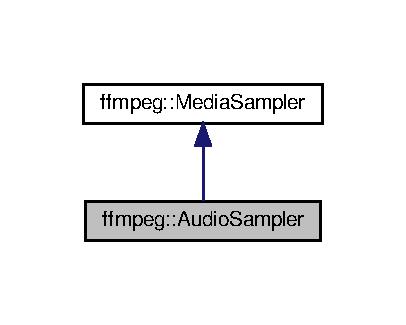
\includegraphics[width=195pt]{classffmpeg_1_1AudioSampler__inherit__graph}
\end{center}
\end{figure}


Collaboration diagram for ffmpeg\+:\+:Audio\+Sampler\+:
\nopagebreak
\begin{figure}[H]
\begin{center}
\leavevmode
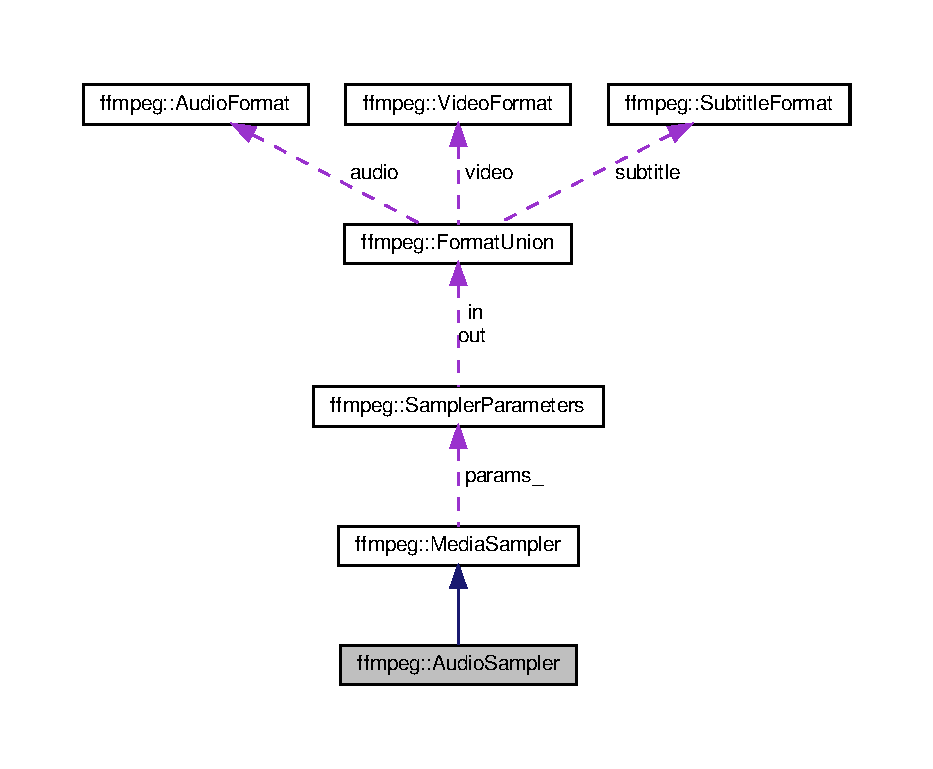
\includegraphics[width=350pt]{classffmpeg_1_1AudioSampler__coll__graph}
\end{center}
\end{figure}
\subsection*{Public Member Functions}
\begin{DoxyCompactItemize}
\item 
\mbox{\Hypertarget{classffmpeg_1_1AudioSampler_ae7fd59e065f7f827bdf164ccfa80dc56}\label{classffmpeg_1_1AudioSampler_ae7fd59e065f7f827bdf164ccfa80dc56}} 
{\bfseries Audio\+Sampler} (void $\ast$log\+Ctx)
\item 
bool \hyperlink{classffmpeg_1_1AudioSampler_a90df92f5b3a265e0cfa9ee44d9e8871b}{init} (const \hyperlink{structffmpeg_1_1SamplerParameters}{Sampler\+Parameters} \&params) override
\item 
int \hyperlink{classffmpeg_1_1AudioSampler_a2188529ebad9ef4593a5ab11e8236989}{sample} (const \hyperlink{classffmpeg_1_1ByteStorage}{Byte\+Storage} $\ast$in, \hyperlink{classffmpeg_1_1ByteStorage}{Byte\+Storage} $\ast$out) override
\item 
void \hyperlink{classffmpeg_1_1AudioSampler_a703ec8da8cc9e6e9701bed75cbc40085}{shutdown} () override
\item 
\mbox{\Hypertarget{classffmpeg_1_1AudioSampler_ab7ac3c8e9a0c6cc1984057ee0307b732}\label{classffmpeg_1_1AudioSampler_ab7ac3c8e9a0c6cc1984057ee0307b732}} 
int {\bfseries sample} (A\+V\+Frame $\ast$frame, \hyperlink{classffmpeg_1_1ByteStorage}{Byte\+Storage} $\ast$out)
\end{DoxyCompactItemize}
\subsection*{Additional Inherited Members}


\subsection{Detailed Description}
Class transcode audio frames from one format into another 

Definition at line 11 of file audio\+\_\+sampler.\+h.



\subsection{Member Function Documentation}
\mbox{\Hypertarget{classffmpeg_1_1AudioSampler_a90df92f5b3a265e0cfa9ee44d9e8871b}\label{classffmpeg_1_1AudioSampler_a90df92f5b3a265e0cfa9ee44d9e8871b}} 
\index{ffmpeg\+::\+Audio\+Sampler@{ffmpeg\+::\+Audio\+Sampler}!init@{init}}
\index{init@{init}!ffmpeg\+::\+Audio\+Sampler@{ffmpeg\+::\+Audio\+Sampler}}
\subsubsection{\texorpdfstring{init()}{init()}}
{\footnotesize\ttfamily bool ffmpeg\+::\+Audio\+Sampler\+::init (\begin{DoxyParamCaption}\item[{const \hyperlink{structffmpeg_1_1SamplerParameters}{Sampler\+Parameters} \&}]{params }\end{DoxyParamCaption})\hspace{0.3cm}{\ttfamily [override]}, {\ttfamily [virtual]}}

Initializes media sampler with parameters 

Implements \hyperlink{classffmpeg_1_1MediaSampler_a049962d62fc930c67d6cf5aa89ae1948}{ffmpeg\+::\+Media\+Sampler}.



Definition at line 43 of file audio\+\_\+sampler.\+cpp.

\mbox{\Hypertarget{classffmpeg_1_1AudioSampler_a2188529ebad9ef4593a5ab11e8236989}\label{classffmpeg_1_1AudioSampler_a2188529ebad9ef4593a5ab11e8236989}} 
\index{ffmpeg\+::\+Audio\+Sampler@{ffmpeg\+::\+Audio\+Sampler}!sample@{sample}}
\index{sample@{sample}!ffmpeg\+::\+Audio\+Sampler@{ffmpeg\+::\+Audio\+Sampler}}
\subsubsection{\texorpdfstring{sample()}{sample()}}
{\footnotesize\ttfamily int ffmpeg\+::\+Audio\+Sampler\+::sample (\begin{DoxyParamCaption}\item[{const \hyperlink{classffmpeg_1_1ByteStorage}{Byte\+Storage} $\ast$}]{in,  }\item[{\hyperlink{classffmpeg_1_1ByteStorage}{Byte\+Storage} $\ast$}]{out }\end{DoxyParamCaption})\hspace{0.3cm}{\ttfamily [override]}, {\ttfamily [virtual]}}

Samples media bytes Returns error code $<$ 0, or $>$=0 -\/ for success, indicating number of bytes processed. set  to null for flushing data 

Implements \hyperlink{classffmpeg_1_1MediaSampler_a1e13816018edada455769f027cf5e9dd}{ffmpeg\+::\+Media\+Sampler}.



Definition at line 198 of file audio\+\_\+sampler.\+cpp.

\mbox{\Hypertarget{classffmpeg_1_1AudioSampler_a703ec8da8cc9e6e9701bed75cbc40085}\label{classffmpeg_1_1AudioSampler_a703ec8da8cc9e6e9701bed75cbc40085}} 
\index{ffmpeg\+::\+Audio\+Sampler@{ffmpeg\+::\+Audio\+Sampler}!shutdown@{shutdown}}
\index{shutdown@{shutdown}!ffmpeg\+::\+Audio\+Sampler@{ffmpeg\+::\+Audio\+Sampler}}
\subsubsection{\texorpdfstring{shutdown()}{shutdown()}}
{\footnotesize\ttfamily void ffmpeg\+::\+Audio\+Sampler\+::shutdown (\begin{DoxyParamCaption}{ }\end{DoxyParamCaption})\hspace{0.3cm}{\ttfamily [override]}, {\ttfamily [virtual]}}

Releases resources 

Implements \hyperlink{classffmpeg_1_1MediaSampler_ac8f2fee9cdf896871776a8202d70edd7}{ffmpeg\+::\+Media\+Sampler}.



Definition at line 39 of file audio\+\_\+sampler.\+cpp.



The documentation for this class was generated from the following files\+:\begin{DoxyCompactItemize}
\item 
/home/jose/ros\+\_\+ws/src/gr\+\_\+perception/gr\+\_\+ml/nb/vision/torchvision/csrc/cpu/decoder/audio\+\_\+sampler.\+h\item 
/home/jose/ros\+\_\+ws/src/gr\+\_\+perception/gr\+\_\+ml/nb/vision/torchvision/csrc/cpu/decoder/audio\+\_\+sampler.\+cpp\end{DoxyCompactItemize}

\hypertarget{classffmpeg_1_1AudioStream}{}\section{ffmpeg\+:\+:Audio\+Stream Class Reference}
\label{classffmpeg_1_1AudioStream}\index{ffmpeg\+::\+Audio\+Stream@{ffmpeg\+::\+Audio\+Stream}}


{\ttfamily \#include $<$audio\+\_\+stream.\+h$>$}



Inheritance diagram for ffmpeg\+:\+:Audio\+Stream\+:
\nopagebreak
\begin{figure}[H]
\begin{center}
\leavevmode
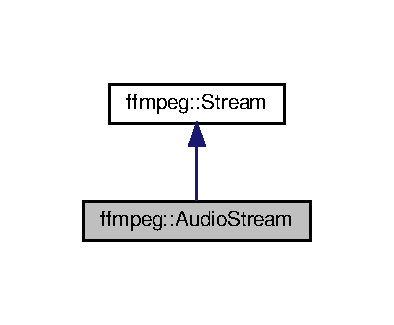
\includegraphics[width=189pt]{classffmpeg_1_1AudioStream__inherit__graph}
\end{center}
\end{figure}


Collaboration diagram for ffmpeg\+:\+:Audio\+Stream\+:
\nopagebreak
\begin{figure}[H]
\begin{center}
\leavevmode
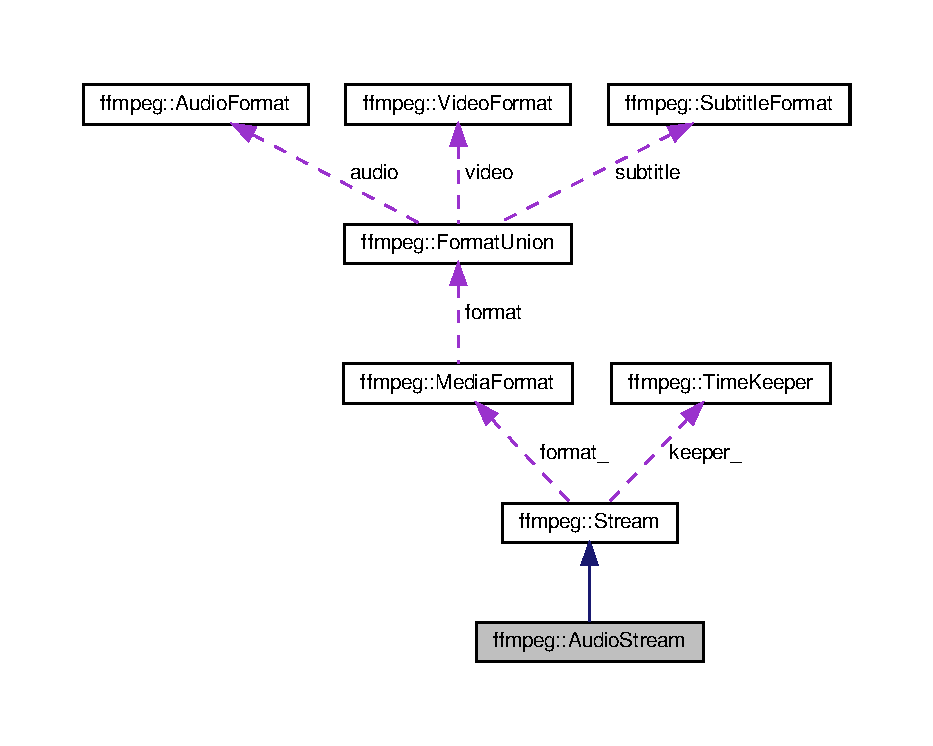
\includegraphics[width=350pt]{classffmpeg_1_1AudioStream__coll__graph}
\end{center}
\end{figure}
\subsection*{Public Member Functions}
\begin{DoxyCompactItemize}
\item 
\mbox{\Hypertarget{classffmpeg_1_1AudioStream_a66445b51a0f02d98ce323e0f0ec4c861}\label{classffmpeg_1_1AudioStream_a66445b51a0f02d98ce323e0f0ec4c861}} 
{\bfseries Audio\+Stream} (A\+V\+Format\+Context $\ast$input\+Ctx, int index, bool convert\+Pts\+To\+Wall\+Time, const \hyperlink{structffmpeg_1_1AudioFormat}{Audio\+Format} \&format)
\end{DoxyCompactItemize}
\subsection*{Additional Inherited Members}


\subsection{Detailed Description}
Class uses F\+F\+M\+P\+EG library to decode one audio stream. 

Definition at line 12 of file audio\+\_\+stream.\+h.



The documentation for this class was generated from the following files\+:\begin{DoxyCompactItemize}
\item 
/home/jose/ros\+\_\+ws/src/gr\+\_\+perception/gr\+\_\+ml/nb/vision/torchvision/csrc/cpu/decoder/audio\+\_\+stream.\+h\item 
/home/jose/ros\+\_\+ws/src/gr\+\_\+perception/gr\+\_\+ml/nb/vision/torchvision/csrc/cpu/decoder/audio\+\_\+stream.\+cpp\end{DoxyCompactItemize}

\hypertarget{classffmpeg_1_1SyncDecoder_1_1AVByteStorage}{}\section{ffmpeg\+:\+:Sync\+Decoder\+:\+:A\+V\+Byte\+Storage Class Reference}
\label{classffmpeg_1_1SyncDecoder_1_1AVByteStorage}\index{ffmpeg\+::\+Sync\+Decoder\+::\+A\+V\+Byte\+Storage@{ffmpeg\+::\+Sync\+Decoder\+::\+A\+V\+Byte\+Storage}}


Inheritance diagram for ffmpeg\+:\+:Sync\+Decoder\+:\+:A\+V\+Byte\+Storage\+:
\nopagebreak
\begin{figure}[H]
\begin{center}
\leavevmode
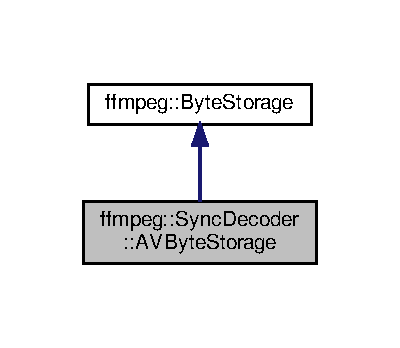
\includegraphics[width=192pt]{classffmpeg_1_1SyncDecoder_1_1AVByteStorage__inherit__graph}
\end{center}
\end{figure}


Collaboration diagram for ffmpeg\+:\+:Sync\+Decoder\+:\+:A\+V\+Byte\+Storage\+:
\nopagebreak
\begin{figure}[H]
\begin{center}
\leavevmode
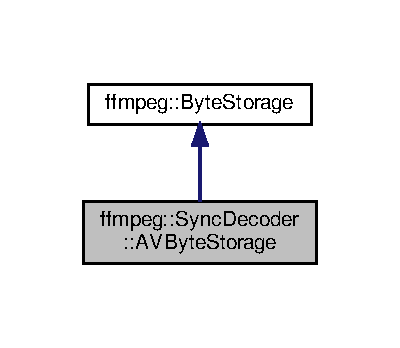
\includegraphics[width=192pt]{classffmpeg_1_1SyncDecoder_1_1AVByteStorage__coll__graph}
\end{center}
\end{figure}
\subsection*{Public Member Functions}
\begin{DoxyCompactItemize}
\item 
\mbox{\Hypertarget{classffmpeg_1_1SyncDecoder_1_1AVByteStorage_a06f8d239442dc4a7a6c52e8e174f1e63}\label{classffmpeg_1_1SyncDecoder_1_1AVByteStorage_a06f8d239442dc4a7a6c52e8e174f1e63}} 
{\bfseries A\+V\+Byte\+Storage} (size\+\_\+t n)
\item 
\mbox{\Hypertarget{classffmpeg_1_1SyncDecoder_1_1AVByteStorage_ade5e0584eeeaba3f46b0e5beeabc49cb}\label{classffmpeg_1_1SyncDecoder_1_1AVByteStorage_ade5e0584eeeaba3f46b0e5beeabc49cb}} 
void {\bfseries ensure} (size\+\_\+t n) override
\item 
\mbox{\Hypertarget{classffmpeg_1_1SyncDecoder_1_1AVByteStorage_a8023ac599c6bec5097c4f87fa386f84c}\label{classffmpeg_1_1SyncDecoder_1_1AVByteStorage_a8023ac599c6bec5097c4f87fa386f84c}} 
uint8\+\_\+t $\ast$ {\bfseries writable\+Tail} () override
\item 
\mbox{\Hypertarget{classffmpeg_1_1SyncDecoder_1_1AVByteStorage_ab1a492096bb7afb8e1c1b229a6beb257}\label{classffmpeg_1_1SyncDecoder_1_1AVByteStorage_ab1a492096bb7afb8e1c1b229a6beb257}} 
void {\bfseries append} (size\+\_\+t n) override
\item 
\mbox{\Hypertarget{classffmpeg_1_1SyncDecoder_1_1AVByteStorage_a52cfe841ffe225fcf279cd549a432930}\label{classffmpeg_1_1SyncDecoder_1_1AVByteStorage_a52cfe841ffe225fcf279cd549a432930}} 
void {\bfseries trim} (size\+\_\+t n) override
\item 
\mbox{\Hypertarget{classffmpeg_1_1SyncDecoder_1_1AVByteStorage_a3dd0a6aabceb74cce0f598d10dfc8fea}\label{classffmpeg_1_1SyncDecoder_1_1AVByteStorage_a3dd0a6aabceb74cce0f598d10dfc8fea}} 
const uint8\+\_\+t $\ast$ {\bfseries data} () const override
\item 
\mbox{\Hypertarget{classffmpeg_1_1SyncDecoder_1_1AVByteStorage_a3d003e88b0058d994635abd81f542e77}\label{classffmpeg_1_1SyncDecoder_1_1AVByteStorage_a3d003e88b0058d994635abd81f542e77}} 
size\+\_\+t {\bfseries length} () const override
\item 
\mbox{\Hypertarget{classffmpeg_1_1SyncDecoder_1_1AVByteStorage_a088eb08d4731687b983000ba055a36c1}\label{classffmpeg_1_1SyncDecoder_1_1AVByteStorage_a088eb08d4731687b983000ba055a36c1}} 
size\+\_\+t {\bfseries tail} () const override
\item 
\mbox{\Hypertarget{classffmpeg_1_1SyncDecoder_1_1AVByteStorage_a41bc484c43425b0c5da42023ffb5990b}\label{classffmpeg_1_1SyncDecoder_1_1AVByteStorage_a41bc484c43425b0c5da42023ffb5990b}} 
void {\bfseries clear} () override
\end{DoxyCompactItemize}


\subsection{Detailed Description}


Definition at line 16 of file sync\+\_\+decoder.\+h.



The documentation for this class was generated from the following files\+:\begin{DoxyCompactItemize}
\item 
/home/jose/ros\+\_\+ws/src/gr\+\_\+perception/gr\+\_\+ml/nb/vision/torchvision/csrc/cpu/decoder/sync\+\_\+decoder.\+h\item 
/home/jose/ros\+\_\+ws/src/gr\+\_\+perception/gr\+\_\+ml/nb/vision/torchvision/csrc/cpu/decoder/sync\+\_\+decoder.\+cpp\end{DoxyCompactItemize}

\hypertarget{structffmpeg_1_1AVSubtitleKeeper}{}\section{ffmpeg\+:\+:A\+V\+Subtitle\+Keeper Struct Reference}
\label{structffmpeg_1_1AVSubtitleKeeper}\index{ffmpeg\+::\+A\+V\+Subtitle\+Keeper@{ffmpeg\+::\+A\+V\+Subtitle\+Keeper}}


{\ttfamily \#include $<$subtitle\+\_\+stream.\+h$>$}



Inheritance diagram for ffmpeg\+:\+:A\+V\+Subtitle\+Keeper\+:
\nopagebreak
\begin{figure}[H]
\begin{center}
\leavevmode
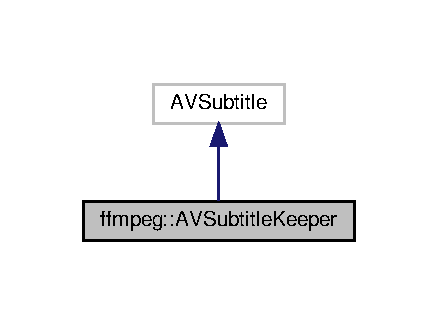
\includegraphics[width=210pt]{structffmpeg_1_1AVSubtitleKeeper__inherit__graph}
\end{center}
\end{figure}


Collaboration diagram for ffmpeg\+:\+:A\+V\+Subtitle\+Keeper\+:
\nopagebreak
\begin{figure}[H]
\begin{center}
\leavevmode
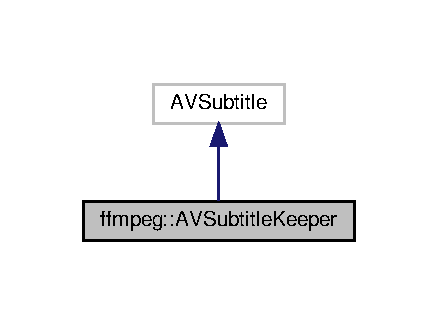
\includegraphics[width=210pt]{structffmpeg_1_1AVSubtitleKeeper__coll__graph}
\end{center}
\end{figure}
\subsection*{Data Fields}
\begin{DoxyCompactItemize}
\item 
\mbox{\Hypertarget{structffmpeg_1_1AVSubtitleKeeper_af894779e5247a33c67900537effa462d}\label{structffmpeg_1_1AVSubtitleKeeper_af894779e5247a33c67900537effa462d}} 
int64\+\_\+t {\bfseries release} \{0\}
\end{DoxyCompactItemize}


\subsection{Detailed Description}
Class uses F\+F\+M\+P\+EG library to decode one subtitle stream. 

Definition at line 11 of file subtitle\+\_\+stream.\+h.



The documentation for this struct was generated from the following file\+:\begin{DoxyCompactItemize}
\item 
/home/jose/ros\+\_\+ws/src/gr\+\_\+perception/gr\+\_\+ml/nb/vision/torchvision/csrc/cpu/decoder/subtitle\+\_\+stream.\+h\end{DoxyCompactItemize}

\hypertarget{classtorchvision_1_1models_1_1detection_1_1backbone__utils_1_1BackboneWithFPN}{}\section{torchvision.\+models.\+detection.\+backbone\+\_\+utils.\+Backbone\+With\+F\+PN Class Reference}
\label{classtorchvision_1_1models_1_1detection_1_1backbone__utils_1_1BackboneWithFPN}\index{torchvision.\+models.\+detection.\+backbone\+\_\+utils.\+Backbone\+With\+F\+PN@{torchvision.\+models.\+detection.\+backbone\+\_\+utils.\+Backbone\+With\+F\+PN}}


Inheritance diagram for torchvision.\+models.\+detection.\+backbone\+\_\+utils.\+Backbone\+With\+F\+PN\+:
\nopagebreak
\begin{figure}[H]
\begin{center}
\leavevmode
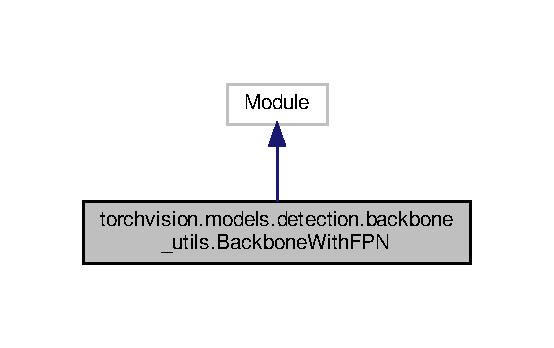
\includegraphics[width=266pt]{classtorchvision_1_1models_1_1detection_1_1backbone__utils_1_1BackboneWithFPN__inherit__graph}
\end{center}
\end{figure}


Collaboration diagram for torchvision.\+models.\+detection.\+backbone\+\_\+utils.\+Backbone\+With\+F\+PN\+:
\nopagebreak
\begin{figure}[H]
\begin{center}
\leavevmode
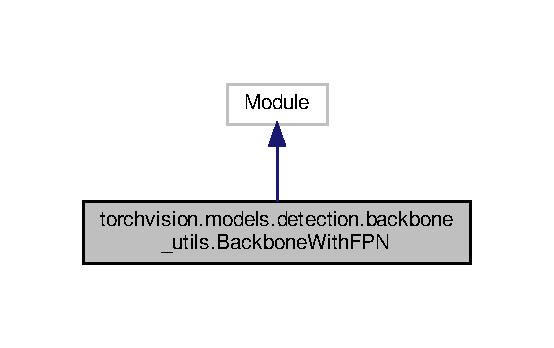
\includegraphics[width=266pt]{classtorchvision_1_1models_1_1detection_1_1backbone__utils_1_1BackboneWithFPN__coll__graph}
\end{center}
\end{figure}
\subsection*{Public Member Functions}
\begin{DoxyCompactItemize}
\item 
\mbox{\Hypertarget{classtorchvision_1_1models_1_1detection_1_1backbone__utils_1_1BackboneWithFPN_a15ed5d7a3170ea7bfdbc5f7331ae9a93}\label{classtorchvision_1_1models_1_1detection_1_1backbone__utils_1_1BackboneWithFPN_a15ed5d7a3170ea7bfdbc5f7331ae9a93}} 
def {\bfseries \+\_\+\+\_\+init\+\_\+\+\_\+} (self, backbone, return\+\_\+layers, in\+\_\+channels\+\_\+list, out\+\_\+channels)
\item 
\mbox{\Hypertarget{classtorchvision_1_1models_1_1detection_1_1backbone__utils_1_1BackboneWithFPN_a61fa7604d615c28e3cca6d888feab3dd}\label{classtorchvision_1_1models_1_1detection_1_1backbone__utils_1_1BackboneWithFPN_a61fa7604d615c28e3cca6d888feab3dd}} 
def {\bfseries forward} (self, x)
\end{DoxyCompactItemize}
\subsection*{Data Fields}
\begin{DoxyCompactItemize}
\item 
\mbox{\Hypertarget{classtorchvision_1_1models_1_1detection_1_1backbone__utils_1_1BackboneWithFPN_ab9ff2b0e9b23909d6220888fb78aced1}\label{classtorchvision_1_1models_1_1detection_1_1backbone__utils_1_1BackboneWithFPN_ab9ff2b0e9b23909d6220888fb78aced1}} 
{\bfseries body}
\item 
\mbox{\Hypertarget{classtorchvision_1_1models_1_1detection_1_1backbone__utils_1_1BackboneWithFPN_ad8c27f9174a83bf374a352e5c986be65}\label{classtorchvision_1_1models_1_1detection_1_1backbone__utils_1_1BackboneWithFPN_ad8c27f9174a83bf374a352e5c986be65}} 
{\bfseries fpn}
\item 
\mbox{\Hypertarget{classtorchvision_1_1models_1_1detection_1_1backbone__utils_1_1BackboneWithFPN_ab2a801040f4464c23f16aa1c2cf0ef7e}\label{classtorchvision_1_1models_1_1detection_1_1backbone__utils_1_1BackboneWithFPN_ab2a801040f4464c23f16aa1c2cf0ef7e}} 
{\bfseries out\+\_\+channels}
\end{DoxyCompactItemize}


\subsection{Detailed Description}
\begin{DoxyVerb}Adds a FPN on top of a model.
Internally, it uses torchvision.models._utils.IntermediateLayerGetter to
extract a submodel that returns the feature maps specified in return_layers.
The same limitations of IntermediatLayerGetter apply here.
Arguments:
    backbone (nn.Module)
    return_layers (Dict[name, new_name]): a dict containing the names
        of the modules for which the activations will be returned as
        the key of the dict, and the value of the dict is the name
        of the returned activation (which the user can specify).
    in_channels_list (List[int]): number of channels for each feature map
        that is returned, in the order they are present in the OrderedDict
    out_channels (int): number of channels in the FPN.
Attributes:
    out_channels (int): the number of channels in the FPN
\end{DoxyVerb}
 

Definition at line 10 of file backbone\+\_\+utils.\+py.



The documentation for this class was generated from the following file\+:\begin{DoxyCompactItemize}
\item 
/home/jose/ros\+\_\+ws/src/gr\+\_\+perception/gr\+\_\+ml/nb/vision/torchvision/models/detection/backbone\+\_\+utils.\+py\end{DoxyCompactItemize}

\hypertarget{classtorchvision_1_1models_1_1detection_1_1__utils_1_1BalancedPositiveNegativeSampler}{}\section{torchvision.\+models.\+detection.\+\_\+utils.\+Balanced\+Positive\+Negative\+Sampler Class Reference}
\label{classtorchvision_1_1models_1_1detection_1_1__utils_1_1BalancedPositiveNegativeSampler}\index{torchvision.\+models.\+detection.\+\_\+utils.\+Balanced\+Positive\+Negative\+Sampler@{torchvision.\+models.\+detection.\+\_\+utils.\+Balanced\+Positive\+Negative\+Sampler}}


Inheritance diagram for torchvision.\+models.\+detection.\+\_\+utils.\+Balanced\+Positive\+Negative\+Sampler\+:
\nopagebreak
\begin{figure}[H]
\begin{center}
\leavevmode
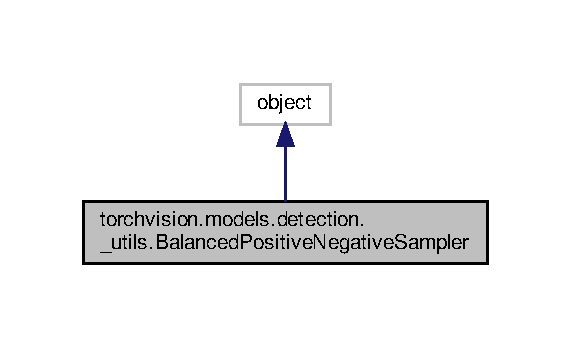
\includegraphics[width=274pt]{classtorchvision_1_1models_1_1detection_1_1__utils_1_1BalancedPositiveNegativeSampler__inherit__graph}
\end{center}
\end{figure}


Collaboration diagram for torchvision.\+models.\+detection.\+\_\+utils.\+Balanced\+Positive\+Negative\+Sampler\+:
\nopagebreak
\begin{figure}[H]
\begin{center}
\leavevmode
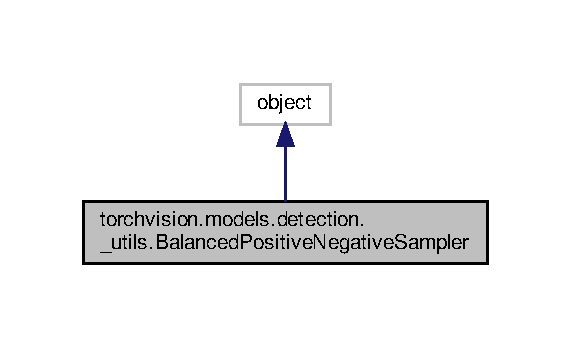
\includegraphics[width=274pt]{classtorchvision_1_1models_1_1detection_1_1__utils_1_1BalancedPositiveNegativeSampler__coll__graph}
\end{center}
\end{figure}
\subsection*{Public Member Functions}
\begin{DoxyCompactItemize}
\item 
def \hyperlink{classtorchvision_1_1models_1_1detection_1_1__utils_1_1BalancedPositiveNegativeSampler_a278a8a8ef3a6ca92eddbbeaafb82ee54}{\+\_\+\+\_\+init\+\_\+\+\_\+} (self, batch\+\_\+size\+\_\+per\+\_\+image, positive\+\_\+fraction)
\item 
def \hyperlink{classtorchvision_1_1models_1_1detection_1_1__utils_1_1BalancedPositiveNegativeSampler_a0c143b41388d87ce90a73e0e0c3f477c}{\+\_\+\+\_\+call\+\_\+\+\_\+} (self, matched\+\_\+idxs)
\end{DoxyCompactItemize}
\subsection*{Data Fields}
\begin{DoxyCompactItemize}
\item 
\mbox{\Hypertarget{classtorchvision_1_1models_1_1detection_1_1__utils_1_1BalancedPositiveNegativeSampler_aa83be68e7b1c540d13fa796c86429b66}\label{classtorchvision_1_1models_1_1detection_1_1__utils_1_1BalancedPositiveNegativeSampler_aa83be68e7b1c540d13fa796c86429b66}} 
{\bfseries batch\+\_\+size\+\_\+per\+\_\+image}
\item 
\mbox{\Hypertarget{classtorchvision_1_1models_1_1detection_1_1__utils_1_1BalancedPositiveNegativeSampler_a143d4b7f14f96b223fedac1ad018273a}\label{classtorchvision_1_1models_1_1detection_1_1__utils_1_1BalancedPositiveNegativeSampler_a143d4b7f14f96b223fedac1ad018273a}} 
{\bfseries positive\+\_\+fraction}
\end{DoxyCompactItemize}


\subsection{Detailed Description}
\begin{DoxyVerb}This class samples batches, ensuring that they contain a fixed proportion of positives
\end{DoxyVerb}
 

Definition at line 9 of file \+\_\+utils.\+py.



\subsection{Constructor \& Destructor Documentation}
\mbox{\Hypertarget{classtorchvision_1_1models_1_1detection_1_1__utils_1_1BalancedPositiveNegativeSampler_a278a8a8ef3a6ca92eddbbeaafb82ee54}\label{classtorchvision_1_1models_1_1detection_1_1__utils_1_1BalancedPositiveNegativeSampler_a278a8a8ef3a6ca92eddbbeaafb82ee54}} 
\index{torchvision\+::models\+::detection\+::\+\_\+utils\+::\+Balanced\+Positive\+Negative\+Sampler@{torchvision\+::models\+::detection\+::\+\_\+utils\+::\+Balanced\+Positive\+Negative\+Sampler}!\+\_\+\+\_\+init\+\_\+\+\_\+@{\+\_\+\+\_\+init\+\_\+\+\_\+}}
\index{\+\_\+\+\_\+init\+\_\+\+\_\+@{\+\_\+\+\_\+init\+\_\+\+\_\+}!torchvision\+::models\+::detection\+::\+\_\+utils\+::\+Balanced\+Positive\+Negative\+Sampler@{torchvision\+::models\+::detection\+::\+\_\+utils\+::\+Balanced\+Positive\+Negative\+Sampler}}
\subsubsection{\texorpdfstring{\+\_\+\+\_\+init\+\_\+\+\_\+()}{\_\_init\_\_()}}
{\footnotesize\ttfamily def torchvision.\+models.\+detection.\+\_\+utils.\+Balanced\+Positive\+Negative\+Sampler.\+\_\+\+\_\+init\+\_\+\+\_\+ (\begin{DoxyParamCaption}\item[{}]{self,  }\item[{}]{batch\+\_\+size\+\_\+per\+\_\+image,  }\item[{}]{positive\+\_\+fraction }\end{DoxyParamCaption})}

\begin{DoxyVerb}Arguments:
    batch_size_per_image (int): number of elements to be selected per image
    positive_fraction (float): percentace of positive elements per batch
\end{DoxyVerb}
 

Definition at line 14 of file \+\_\+utils.\+py.



\subsection{Member Function Documentation}
\mbox{\Hypertarget{classtorchvision_1_1models_1_1detection_1_1__utils_1_1BalancedPositiveNegativeSampler_a0c143b41388d87ce90a73e0e0c3f477c}\label{classtorchvision_1_1models_1_1detection_1_1__utils_1_1BalancedPositiveNegativeSampler_a0c143b41388d87ce90a73e0e0c3f477c}} 
\index{torchvision\+::models\+::detection\+::\+\_\+utils\+::\+Balanced\+Positive\+Negative\+Sampler@{torchvision\+::models\+::detection\+::\+\_\+utils\+::\+Balanced\+Positive\+Negative\+Sampler}!\+\_\+\+\_\+call\+\_\+\+\_\+@{\+\_\+\+\_\+call\+\_\+\+\_\+}}
\index{\+\_\+\+\_\+call\+\_\+\+\_\+@{\+\_\+\+\_\+call\+\_\+\+\_\+}!torchvision\+::models\+::detection\+::\+\_\+utils\+::\+Balanced\+Positive\+Negative\+Sampler@{torchvision\+::models\+::detection\+::\+\_\+utils\+::\+Balanced\+Positive\+Negative\+Sampler}}
\subsubsection{\texorpdfstring{\+\_\+\+\_\+call\+\_\+\+\_\+()}{\_\_call\_\_()}}
{\footnotesize\ttfamily def torchvision.\+models.\+detection.\+\_\+utils.\+Balanced\+Positive\+Negative\+Sampler.\+\_\+\+\_\+call\+\_\+\+\_\+ (\begin{DoxyParamCaption}\item[{}]{self,  }\item[{}]{matched\+\_\+idxs }\end{DoxyParamCaption})}

\begin{DoxyVerb}Arguments:
    matched idxs: list of tensors containing -1, 0 or positive values.
Each tensor corresponds to a specific image.
-1 values are ignored, 0 are considered as negatives and > 0 as
positives.

Returns:
    pos_idx (list[tensor])
    neg_idx (list[tensor])

Returns two lists of binary masks for each image.
The first list contains the positive elements that were selected,
and the second list the negative example.
\end{DoxyVerb}
 

Definition at line 24 of file \+\_\+utils.\+py.



The documentation for this class was generated from the following file\+:\begin{DoxyCompactItemize}
\item 
/home/jose/ros\+\_\+ws/src/gr\+\_\+perception/gr\+\_\+ml/nb/vision/torchvision/models/detection/\+\_\+utils.\+py\end{DoxyCompactItemize}

\hypertarget{classtorchvision_1_1models_1_1resnet_1_1BasicBlock}{}\section{torchvision.\+models.\+resnet.\+Basic\+Block Class Reference}
\label{classtorchvision_1_1models_1_1resnet_1_1BasicBlock}\index{torchvision.\+models.\+resnet.\+Basic\+Block@{torchvision.\+models.\+resnet.\+Basic\+Block}}


Inheritance diagram for torchvision.\+models.\+resnet.\+Basic\+Block\+:
\nopagebreak
\begin{figure}[H]
\begin{center}
\leavevmode
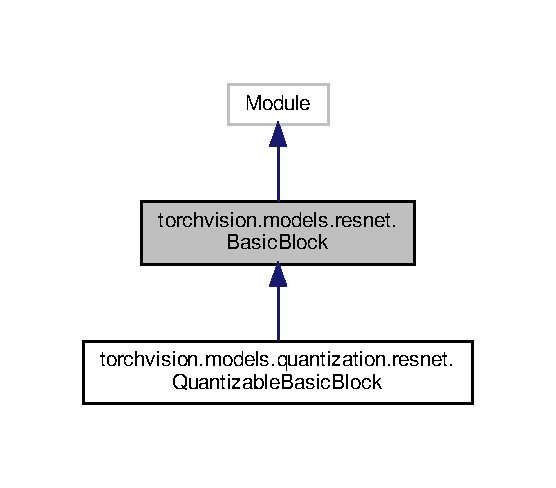
\includegraphics[width=267pt]{classtorchvision_1_1models_1_1resnet_1_1BasicBlock__inherit__graph}
\end{center}
\end{figure}


Collaboration diagram for torchvision.\+models.\+resnet.\+Basic\+Block\+:
\nopagebreak
\begin{figure}[H]
\begin{center}
\leavevmode
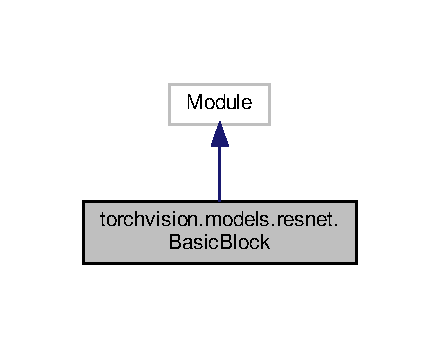
\includegraphics[width=211pt]{classtorchvision_1_1models_1_1resnet_1_1BasicBlock__coll__graph}
\end{center}
\end{figure}
\subsection*{Public Member Functions}
\begin{DoxyCompactItemize}
\item 
\mbox{\Hypertarget{classtorchvision_1_1models_1_1resnet_1_1BasicBlock_a19b9990ff0708e9376c1658fc59262d9}\label{classtorchvision_1_1models_1_1resnet_1_1BasicBlock_a19b9990ff0708e9376c1658fc59262d9}} 
def {\bfseries \+\_\+\+\_\+init\+\_\+\+\_\+} (self, inplanes, planes, stride=1, downsample=None, groups=1, base\+\_\+width=64, dilation=1, norm\+\_\+layer=None)
\item 
\mbox{\Hypertarget{classtorchvision_1_1models_1_1resnet_1_1BasicBlock_a535ad6f9a377ab5d4a0b675b15c4eb70}\label{classtorchvision_1_1models_1_1resnet_1_1BasicBlock_a535ad6f9a377ab5d4a0b675b15c4eb70}} 
def {\bfseries forward} (self, x)
\end{DoxyCompactItemize}
\subsection*{Data Fields}
\begin{DoxyCompactItemize}
\item 
\mbox{\Hypertarget{classtorchvision_1_1models_1_1resnet_1_1BasicBlock_a3ffc18976e7b76dd0ebd121d6b40ccb2}\label{classtorchvision_1_1models_1_1resnet_1_1BasicBlock_a3ffc18976e7b76dd0ebd121d6b40ccb2}} 
{\bfseries conv1}
\item 
\mbox{\Hypertarget{classtorchvision_1_1models_1_1resnet_1_1BasicBlock_a11e066d7ce11f945652fc89ba8f2cf44}\label{classtorchvision_1_1models_1_1resnet_1_1BasicBlock_a11e066d7ce11f945652fc89ba8f2cf44}} 
{\bfseries bn1}
\item 
\mbox{\Hypertarget{classtorchvision_1_1models_1_1resnet_1_1BasicBlock_a24ce2f557178f1ab11bcea50fa0bc714}\label{classtorchvision_1_1models_1_1resnet_1_1BasicBlock_a24ce2f557178f1ab11bcea50fa0bc714}} 
{\bfseries relu}
\item 
\mbox{\Hypertarget{classtorchvision_1_1models_1_1resnet_1_1BasicBlock_afbdfa6848564c8f5064b93e6cf51301c}\label{classtorchvision_1_1models_1_1resnet_1_1BasicBlock_afbdfa6848564c8f5064b93e6cf51301c}} 
{\bfseries conv2}
\item 
\mbox{\Hypertarget{classtorchvision_1_1models_1_1resnet_1_1BasicBlock_a47e012bbae314c9e2724dc798abb0ad7}\label{classtorchvision_1_1models_1_1resnet_1_1BasicBlock_a47e012bbae314c9e2724dc798abb0ad7}} 
{\bfseries bn2}
\item 
\mbox{\Hypertarget{classtorchvision_1_1models_1_1resnet_1_1BasicBlock_a5ec26277d613fabd295546e0805facbb}\label{classtorchvision_1_1models_1_1resnet_1_1BasicBlock_a5ec26277d613fabd295546e0805facbb}} 
{\bfseries downsample}
\item 
\mbox{\Hypertarget{classtorchvision_1_1models_1_1resnet_1_1BasicBlock_aac05bcf5d7b49524a969d92f3c2f12f2}\label{classtorchvision_1_1models_1_1resnet_1_1BasicBlock_aac05bcf5d7b49524a969d92f3c2f12f2}} 
{\bfseries stride}
\end{DoxyCompactItemize}
\subsection*{Static Public Attributes}
\begin{DoxyCompactItemize}
\item 
\mbox{\Hypertarget{classtorchvision_1_1models_1_1resnet_1_1BasicBlock_ab6c28d9436782a51be57424479d79830}\label{classtorchvision_1_1models_1_1resnet_1_1BasicBlock_ab6c28d9436782a51be57424479d79830}} 
{\bfseries expansion}
\end{DoxyCompactItemize}


\subsection{Detailed Description}


Definition at line 35 of file resnet.\+py.



The documentation for this class was generated from the following file\+:\begin{DoxyCompactItemize}
\item 
/home/jose/ros\+\_\+ws/src/gr\+\_\+perception/gr\+\_\+ml/nb/vision/torchvision/models/resnet.\+py\end{DoxyCompactItemize}

\hypertarget{classtorchvision_1_1models_1_1video_1_1resnet_1_1BasicBlock}{}\section{torchvision.\+models.\+video.\+resnet.\+Basic\+Block Class Reference}
\label{classtorchvision_1_1models_1_1video_1_1resnet_1_1BasicBlock}\index{torchvision.\+models.\+video.\+resnet.\+Basic\+Block@{torchvision.\+models.\+video.\+resnet.\+Basic\+Block}}


Inheritance diagram for torchvision.\+models.\+video.\+resnet.\+Basic\+Block\+:
\nopagebreak
\begin{figure}[H]
\begin{center}
\leavevmode
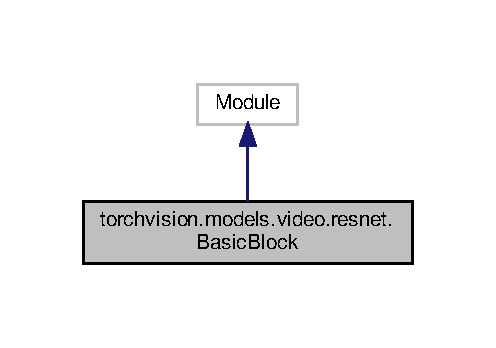
\includegraphics[width=238pt]{classtorchvision_1_1models_1_1video_1_1resnet_1_1BasicBlock__inherit__graph}
\end{center}
\end{figure}


Collaboration diagram for torchvision.\+models.\+video.\+resnet.\+Basic\+Block\+:
\nopagebreak
\begin{figure}[H]
\begin{center}
\leavevmode
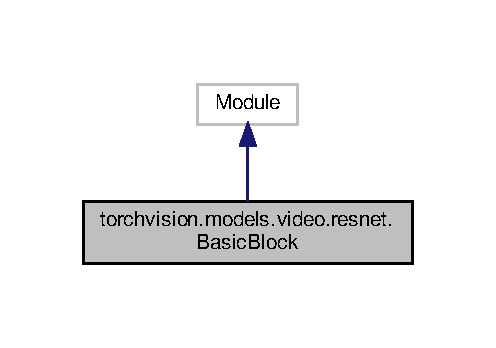
\includegraphics[width=238pt]{classtorchvision_1_1models_1_1video_1_1resnet_1_1BasicBlock__coll__graph}
\end{center}
\end{figure}
\subsection*{Public Member Functions}
\begin{DoxyCompactItemize}
\item 
\mbox{\Hypertarget{classtorchvision_1_1models_1_1video_1_1resnet_1_1BasicBlock_aeab8c9f6c07d72bf7aeb9682688ad68d}\label{classtorchvision_1_1models_1_1video_1_1resnet_1_1BasicBlock_aeab8c9f6c07d72bf7aeb9682688ad68d}} 
def {\bfseries \+\_\+\+\_\+init\+\_\+\+\_\+} (self, inplanes, planes, conv\+\_\+builder, stride=1, downsample=None)
\item 
\mbox{\Hypertarget{classtorchvision_1_1models_1_1video_1_1resnet_1_1BasicBlock_a87ee43bb0854459cdd2b6041c975b86c}\label{classtorchvision_1_1models_1_1video_1_1resnet_1_1BasicBlock_a87ee43bb0854459cdd2b6041c975b86c}} 
def {\bfseries forward} (self, x)
\end{DoxyCompactItemize}
\subsection*{Data Fields}
\begin{DoxyCompactItemize}
\item 
\mbox{\Hypertarget{classtorchvision_1_1models_1_1video_1_1resnet_1_1BasicBlock_ab40bbe234d5ad5095c225c9615dc116a}\label{classtorchvision_1_1models_1_1video_1_1resnet_1_1BasicBlock_ab40bbe234d5ad5095c225c9615dc116a}} 
{\bfseries conv1}
\item 
\mbox{\Hypertarget{classtorchvision_1_1models_1_1video_1_1resnet_1_1BasicBlock_a534381f344c35d0ce752306f096a19ca}\label{classtorchvision_1_1models_1_1video_1_1resnet_1_1BasicBlock_a534381f344c35d0ce752306f096a19ca}} 
{\bfseries conv2}
\item 
\mbox{\Hypertarget{classtorchvision_1_1models_1_1video_1_1resnet_1_1BasicBlock_a8f310312a129b7ddb5198799cca7dc84}\label{classtorchvision_1_1models_1_1video_1_1resnet_1_1BasicBlock_a8f310312a129b7ddb5198799cca7dc84}} 
{\bfseries relu}
\item 
\mbox{\Hypertarget{classtorchvision_1_1models_1_1video_1_1resnet_1_1BasicBlock_aa67c9a516a193bed68076da8e3b7b28d}\label{classtorchvision_1_1models_1_1video_1_1resnet_1_1BasicBlock_aa67c9a516a193bed68076da8e3b7b28d}} 
{\bfseries downsample}
\item 
\mbox{\Hypertarget{classtorchvision_1_1models_1_1video_1_1resnet_1_1BasicBlock_a41395c84c0812d7bb533629e2e953557}\label{classtorchvision_1_1models_1_1video_1_1resnet_1_1BasicBlock_a41395c84c0812d7bb533629e2e953557}} 
{\bfseries stride}
\end{DoxyCompactItemize}
\subsection*{Static Public Attributes}
\begin{DoxyCompactItemize}
\item 
\mbox{\Hypertarget{classtorchvision_1_1models_1_1video_1_1resnet_1_1BasicBlock_a120a0a3f82cca85b248032bd02962267}\label{classtorchvision_1_1models_1_1video_1_1resnet_1_1BasicBlock_a120a0a3f82cca85b248032bd02962267}} 
{\bfseries expansion}
\end{DoxyCompactItemize}


\subsection{Detailed Description}


Definition at line 82 of file resnet.\+py.



The documentation for this class was generated from the following file\+:\begin{DoxyCompactItemize}
\item 
/home/jose/ros\+\_\+ws/src/gr\+\_\+perception/gr\+\_\+ml/nb/vision/torchvision/models/video/resnet.\+py\end{DoxyCompactItemize}

\hypertarget{structvision_1_1models_1_1__resnetimpl_1_1BasicBlock}{}\section{vision\+:\+:models\+:\+:\+\_\+resnetimpl\+:\+:Basic\+Block Struct Reference}
\label{structvision_1_1models_1_1__resnetimpl_1_1BasicBlock}\index{vision\+::models\+::\+\_\+resnetimpl\+::\+Basic\+Block@{vision\+::models\+::\+\_\+resnetimpl\+::\+Basic\+Block}}


Inheritance diagram for vision\+:\+:models\+:\+:\+\_\+resnetimpl\+:\+:Basic\+Block\+:
\nopagebreak
\begin{figure}[H]
\begin{center}
\leavevmode
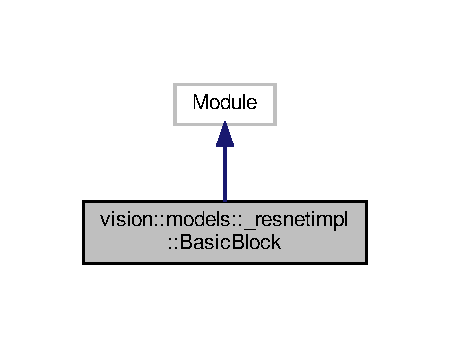
\includegraphics[width=216pt]{structvision_1_1models_1_1__resnetimpl_1_1BasicBlock__inherit__graph}
\end{center}
\end{figure}


Collaboration diagram for vision\+:\+:models\+:\+:\+\_\+resnetimpl\+:\+:Basic\+Block\+:
\nopagebreak
\begin{figure}[H]
\begin{center}
\leavevmode
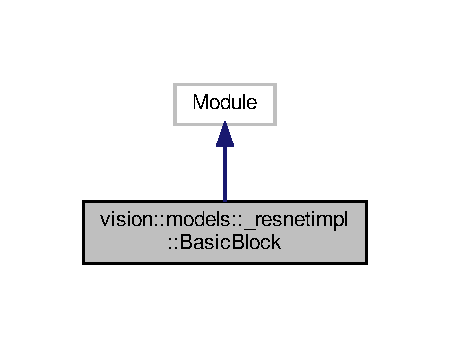
\includegraphics[width=216pt]{structvision_1_1models_1_1__resnetimpl_1_1BasicBlock__coll__graph}
\end{center}
\end{figure}
\subsection*{Public Member Functions}
\begin{DoxyCompactItemize}
\item 
\mbox{\Hypertarget{structvision_1_1models_1_1__resnetimpl_1_1BasicBlock_ab7b6ea8f328046286a9d57421c4351a9}\label{structvision_1_1models_1_1__resnetimpl_1_1BasicBlock_ab7b6ea8f328046286a9d57421c4351a9}} 
{\bfseries Basic\+Block} (int64\+\_\+t inplanes, int64\+\_\+t planes, int64\+\_\+t stride=1, torch\+::nn\+::\+Sequential downsample=nullptr, int64\+\_\+t groups=1, int64\+\_\+t base\+\_\+width=64)
\item 
\mbox{\Hypertarget{structvision_1_1models_1_1__resnetimpl_1_1BasicBlock_a59cb97675123a82bae2e9e837401c5a4}\label{structvision_1_1models_1_1__resnetimpl_1_1BasicBlock_a59cb97675123a82bae2e9e837401c5a4}} 
torch\+::\+Tensor {\bfseries forward} (torch\+::\+Tensor x)
\end{DoxyCompactItemize}
\subsection*{Data Fields}
\begin{DoxyCompactItemize}
\item 
\mbox{\Hypertarget{structvision_1_1models_1_1__resnetimpl_1_1BasicBlock_ac509762f431c11d17eceeacfbec74206}\label{structvision_1_1models_1_1__resnetimpl_1_1BasicBlock_ac509762f431c11d17eceeacfbec74206}} 
int64\+\_\+t {\bfseries stride}
\item 
\mbox{\Hypertarget{structvision_1_1models_1_1__resnetimpl_1_1BasicBlock_ad55164fd51eebe4bcb780aba5435f6e4}\label{structvision_1_1models_1_1__resnetimpl_1_1BasicBlock_ad55164fd51eebe4bcb780aba5435f6e4}} 
torch\+::nn\+::\+Sequential {\bfseries downsample}
\item 
\mbox{\Hypertarget{structvision_1_1models_1_1__resnetimpl_1_1BasicBlock_a66658f06b50efd9456f897a905461097}\label{structvision_1_1models_1_1__resnetimpl_1_1BasicBlock_a66658f06b50efd9456f897a905461097}} 
torch\+::nn\+::\+Conv2d {\bfseries conv1} \{nullptr\}
\item 
\mbox{\Hypertarget{structvision_1_1models_1_1__resnetimpl_1_1BasicBlock_a82b1096c8c891bdfce41f06edb66e210}\label{structvision_1_1models_1_1__resnetimpl_1_1BasicBlock_a82b1096c8c891bdfce41f06edb66e210}} 
torch\+::nn\+::\+Conv2d {\bfseries conv2} \{nullptr\}
\item 
\mbox{\Hypertarget{structvision_1_1models_1_1__resnetimpl_1_1BasicBlock_ad6b514f723aa7d1bd769fd4955ad9e2d}\label{structvision_1_1models_1_1__resnetimpl_1_1BasicBlock_ad6b514f723aa7d1bd769fd4955ad9e2d}} 
torch\+::nn\+::\+Batch\+Norm2d {\bfseries bn1} \{nullptr\}
\item 
\mbox{\Hypertarget{structvision_1_1models_1_1__resnetimpl_1_1BasicBlock_a2c1ed5219ef603198a4096f7a6311f76}\label{structvision_1_1models_1_1__resnetimpl_1_1BasicBlock_a2c1ed5219ef603198a4096f7a6311f76}} 
torch\+::nn\+::\+Batch\+Norm2d {\bfseries bn2} \{nullptr\}
\end{DoxyCompactItemize}
\subsection*{Static Public Attributes}
\begin{DoxyCompactItemize}
\item 
\mbox{\Hypertarget{structvision_1_1models_1_1__resnetimpl_1_1BasicBlock_a56b91d31ad5dc2923186f9fc01aa16b7}\label{structvision_1_1models_1_1__resnetimpl_1_1BasicBlock_a56b91d31ad5dc2923186f9fc01aa16b7}} 
static int {\bfseries expansion} = 1
\end{DoxyCompactItemize}
\subsection*{Friends}
\begin{DoxyCompactItemize}
\item 
\mbox{\Hypertarget{structvision_1_1models_1_1__resnetimpl_1_1BasicBlock_a2d4c95d61d2126a085e162451df61b9d}\label{structvision_1_1models_1_1__resnetimpl_1_1BasicBlock_a2d4c95d61d2126a085e162451df61b9d}} 
{\footnotesize template$<$typename Block $>$ }\\struct {\bfseries vision\+::models\+::\+Res\+Net\+Impl}
\end{DoxyCompactItemize}


\subsection{Detailed Description}


Definition at line 23 of file resnet.\+h.



The documentation for this struct was generated from the following files\+:\begin{DoxyCompactItemize}
\item 
/home/jose/ros\+\_\+ws/src/gr\+\_\+perception/gr\+\_\+ml/nb/vision/torchvision/csrc/models/resnet.\+h\item 
/home/jose/ros\+\_\+ws/src/gr\+\_\+perception/gr\+\_\+ml/nb/vision/torchvision/csrc/models/resnet.\+cpp\end{DoxyCompactItemize}

\hypertarget{classtorchvision_1_1models_1_1googlenet_1_1BasicConv2d}{}\section{torchvision.\+models.\+googlenet.\+Basic\+Conv2d Class Reference}
\label{classtorchvision_1_1models_1_1googlenet_1_1BasicConv2d}\index{torchvision.\+models.\+googlenet.\+Basic\+Conv2d@{torchvision.\+models.\+googlenet.\+Basic\+Conv2d}}


Inheritance diagram for torchvision.\+models.\+googlenet.\+Basic\+Conv2d\+:
\nopagebreak
\begin{figure}[H]
\begin{center}
\leavevmode
\includegraphics[width=282pt]{classtorchvision_1_1models_1_1googlenet_1_1BasicConv2d__inherit__graph}
\end{center}
\end{figure}


Collaboration diagram for torchvision.\+models.\+googlenet.\+Basic\+Conv2d\+:
\nopagebreak
\begin{figure}[H]
\begin{center}
\leavevmode
\includegraphics[width=226pt]{classtorchvision_1_1models_1_1googlenet_1_1BasicConv2d__coll__graph}
\end{center}
\end{figure}
\subsection*{Public Member Functions}
\begin{DoxyCompactItemize}
\item 
\mbox{\Hypertarget{classtorchvision_1_1models_1_1googlenet_1_1BasicConv2d_a4d9cb24f069b26e5f4f362d0ff522da1}\label{classtorchvision_1_1models_1_1googlenet_1_1BasicConv2d_a4d9cb24f069b26e5f4f362d0ff522da1}} 
def {\bfseries \+\_\+\+\_\+init\+\_\+\+\_\+} (self, in\+\_\+channels, out\+\_\+channels, kwargs)
\item 
\mbox{\Hypertarget{classtorchvision_1_1models_1_1googlenet_1_1BasicConv2d_a69d77068dd4eca8935743602e2f2f376}\label{classtorchvision_1_1models_1_1googlenet_1_1BasicConv2d_a69d77068dd4eca8935743602e2f2f376}} 
def {\bfseries forward} (self, x)
\end{DoxyCompactItemize}
\subsection*{Data Fields}
\begin{DoxyCompactItemize}
\item 
\mbox{\Hypertarget{classtorchvision_1_1models_1_1googlenet_1_1BasicConv2d_ac267b5767772bbd9b02dc90053539d2d}\label{classtorchvision_1_1models_1_1googlenet_1_1BasicConv2d_ac267b5767772bbd9b02dc90053539d2d}} 
{\bfseries conv}
\item 
\mbox{\Hypertarget{classtorchvision_1_1models_1_1googlenet_1_1BasicConv2d_a1c054c6202458ef91c51085af7dfc985}\label{classtorchvision_1_1models_1_1googlenet_1_1BasicConv2d_a1c054c6202458ef91c51085af7dfc985}} 
{\bfseries bn}
\end{DoxyCompactItemize}


\subsection{Detailed Description}


Definition at line 285 of file googlenet.\+py.



The documentation for this class was generated from the following file\+:\begin{DoxyCompactItemize}
\item 
/home/jose/ros\+\_\+ws/src/gr\+\_\+perception/gr\+\_\+ml/nb/vision/torchvision/models/googlenet.\+py\end{DoxyCompactItemize}

\hypertarget{classtorchvision_1_1models_1_1inception_1_1BasicConv2d}{}\section{torchvision.\+models.\+inception.\+Basic\+Conv2d Class Reference}
\label{classtorchvision_1_1models_1_1inception_1_1BasicConv2d}\index{torchvision.\+models.\+inception.\+Basic\+Conv2d@{torchvision.\+models.\+inception.\+Basic\+Conv2d}}


Inheritance diagram for torchvision.\+models.\+inception.\+Basic\+Conv2d\+:
\nopagebreak
\begin{figure}[H]
\begin{center}
\leavevmode
\includegraphics[width=223pt]{classtorchvision_1_1models_1_1inception_1_1BasicConv2d__inherit__graph}
\end{center}
\end{figure}


Collaboration diagram for torchvision.\+models.\+inception.\+Basic\+Conv2d\+:
\nopagebreak
\begin{figure}[H]
\begin{center}
\leavevmode
\includegraphics[width=223pt]{classtorchvision_1_1models_1_1inception_1_1BasicConv2d__coll__graph}
\end{center}
\end{figure}
\subsection*{Public Member Functions}
\begin{DoxyCompactItemize}
\item 
\mbox{\Hypertarget{classtorchvision_1_1models_1_1inception_1_1BasicConv2d_a2bd3562317533e3273b0a9f231088b34}\label{classtorchvision_1_1models_1_1inception_1_1BasicConv2d_a2bd3562317533e3273b0a9f231088b34}} 
def {\bfseries \+\_\+\+\_\+init\+\_\+\+\_\+} (self, in\+\_\+channels, out\+\_\+channels, kwargs)
\item 
\mbox{\Hypertarget{classtorchvision_1_1models_1_1inception_1_1BasicConv2d_a83109241cad4317e468635ae9d7cc9cb}\label{classtorchvision_1_1models_1_1inception_1_1BasicConv2d_a83109241cad4317e468635ae9d7cc9cb}} 
def {\bfseries forward} (self, x)
\end{DoxyCompactItemize}
\subsection*{Data Fields}
\begin{DoxyCompactItemize}
\item 
\mbox{\Hypertarget{classtorchvision_1_1models_1_1inception_1_1BasicConv2d_a9d1809e67dfeb1cf55633f92543a7aa2}\label{classtorchvision_1_1models_1_1inception_1_1BasicConv2d_a9d1809e67dfeb1cf55633f92543a7aa2}} 
{\bfseries conv}
\item 
\mbox{\Hypertarget{classtorchvision_1_1models_1_1inception_1_1BasicConv2d_a91f89397952a9db169a5403e5fdf52e6}\label{classtorchvision_1_1models_1_1inception_1_1BasicConv2d_a91f89397952a9db169a5403e5fdf52e6}} 
{\bfseries bn}
\end{DoxyCompactItemize}


\subsection{Detailed Description}


Definition at line 432 of file inception.\+py.



The documentation for this class was generated from the following file\+:\begin{DoxyCompactItemize}
\item 
/home/jose/ros\+\_\+ws/src/gr\+\_\+perception/gr\+\_\+ml/nb/vision/torchvision/models/inception.\+py\end{DoxyCompactItemize}

\hypertarget{structvision_1_1models_1_1__googlenetimpl_1_1BasicConv2dImpl}{}\section{vision\+:\+:models\+:\+:\+\_\+googlenetimpl\+:\+:Basic\+Conv2d\+Impl Struct Reference}
\label{structvision_1_1models_1_1__googlenetimpl_1_1BasicConv2dImpl}\index{vision\+::models\+::\+\_\+googlenetimpl\+::\+Basic\+Conv2d\+Impl@{vision\+::models\+::\+\_\+googlenetimpl\+::\+Basic\+Conv2d\+Impl}}


Inheritance diagram for vision\+:\+:models\+:\+:\+\_\+googlenetimpl\+:\+:Basic\+Conv2d\+Impl\+:
\nopagebreak
\begin{figure}[H]
\begin{center}
\leavevmode
\includegraphics[width=231pt]{structvision_1_1models_1_1__googlenetimpl_1_1BasicConv2dImpl__inherit__graph}
\end{center}
\end{figure}


Collaboration diagram for vision\+:\+:models\+:\+:\+\_\+googlenetimpl\+:\+:Basic\+Conv2d\+Impl\+:
\nopagebreak
\begin{figure}[H]
\begin{center}
\leavevmode
\includegraphics[width=231pt]{structvision_1_1models_1_1__googlenetimpl_1_1BasicConv2dImpl__coll__graph}
\end{center}
\end{figure}
\subsection*{Public Member Functions}
\begin{DoxyCompactItemize}
\item 
\mbox{\Hypertarget{structvision_1_1models_1_1__googlenetimpl_1_1BasicConv2dImpl_abf3ad0ee0573d05655bba86729320733}\label{structvision_1_1models_1_1__googlenetimpl_1_1BasicConv2dImpl_abf3ad0ee0573d05655bba86729320733}} 
{\bfseries Basic\+Conv2d\+Impl} (torch\+::nn\+::\+Conv2d\+Options options)
\item 
\mbox{\Hypertarget{structvision_1_1models_1_1__googlenetimpl_1_1BasicConv2dImpl_a945da35d706b36ff76052523a68bdc35}\label{structvision_1_1models_1_1__googlenetimpl_1_1BasicConv2dImpl_a945da35d706b36ff76052523a68bdc35}} 
torch\+::\+Tensor {\bfseries forward} (torch\+::\+Tensor x)
\end{DoxyCompactItemize}
\subsection*{Data Fields}
\begin{DoxyCompactItemize}
\item 
\mbox{\Hypertarget{structvision_1_1models_1_1__googlenetimpl_1_1BasicConv2dImpl_a0043f4f55bc1666eac1d55eb5578d06f}\label{structvision_1_1models_1_1__googlenetimpl_1_1BasicConv2dImpl_a0043f4f55bc1666eac1d55eb5578d06f}} 
torch\+::nn\+::\+Conv2d {\bfseries conv} \{nullptr\}
\item 
\mbox{\Hypertarget{structvision_1_1models_1_1__googlenetimpl_1_1BasicConv2dImpl_ac73e86e144d48c82517d516000419823}\label{structvision_1_1models_1_1__googlenetimpl_1_1BasicConv2dImpl_ac73e86e144d48c82517d516000419823}} 
torch\+::nn\+::\+Batch\+Norm2d {\bfseries bn} \{nullptr\}
\end{DoxyCompactItemize}


\subsection{Detailed Description}


Definition at line 11 of file googlenet.\+h.



The documentation for this struct was generated from the following files\+:\begin{DoxyCompactItemize}
\item 
/home/jose/ros\+\_\+ws/src/gr\+\_\+perception/gr\+\_\+ml/nb/vision/torchvision/csrc/models/googlenet.\+h\item 
/home/jose/ros\+\_\+ws/src/gr\+\_\+perception/gr\+\_\+ml/nb/vision/torchvision/csrc/models/googlenet.\+cpp\end{DoxyCompactItemize}

\hypertarget{structvision_1_1models_1_1__inceptionimpl_1_1BasicConv2dImpl}{}\section{vision\+:\+:models\+:\+:\+\_\+inceptionimpl\+:\+:Basic\+Conv2d\+Impl Struct Reference}
\label{structvision_1_1models_1_1__inceptionimpl_1_1BasicConv2dImpl}\index{vision\+::models\+::\+\_\+inceptionimpl\+::\+Basic\+Conv2d\+Impl@{vision\+::models\+::\+\_\+inceptionimpl\+::\+Basic\+Conv2d\+Impl}}


Inheritance diagram for vision\+:\+:models\+:\+:\+\_\+inceptionimpl\+:\+:Basic\+Conv2d\+Impl\+:
\nopagebreak
\begin{figure}[H]
\begin{center}
\leavevmode
\includegraphics[width=228pt]{structvision_1_1models_1_1__inceptionimpl_1_1BasicConv2dImpl__inherit__graph}
\end{center}
\end{figure}


Collaboration diagram for vision\+:\+:models\+:\+:\+\_\+inceptionimpl\+:\+:Basic\+Conv2d\+Impl\+:
\nopagebreak
\begin{figure}[H]
\begin{center}
\leavevmode
\includegraphics[width=228pt]{structvision_1_1models_1_1__inceptionimpl_1_1BasicConv2dImpl__coll__graph}
\end{center}
\end{figure}
\subsection*{Public Member Functions}
\begin{DoxyCompactItemize}
\item 
\mbox{\Hypertarget{structvision_1_1models_1_1__inceptionimpl_1_1BasicConv2dImpl_a96bfecb5ffd28f0879721e961caaa9c6}\label{structvision_1_1models_1_1__inceptionimpl_1_1BasicConv2dImpl_a96bfecb5ffd28f0879721e961caaa9c6}} 
{\bfseries Basic\+Conv2d\+Impl} (torch\+::nn\+::\+Conv2d\+Options options, double std\+\_\+dev=0.\+1)
\item 
\mbox{\Hypertarget{structvision_1_1models_1_1__inceptionimpl_1_1BasicConv2dImpl_a7a7a30135a9ea4e72498fb407afc857a}\label{structvision_1_1models_1_1__inceptionimpl_1_1BasicConv2dImpl_a7a7a30135a9ea4e72498fb407afc857a}} 
torch\+::\+Tensor {\bfseries forward} (torch\+::\+Tensor x)
\end{DoxyCompactItemize}
\subsection*{Data Fields}
\begin{DoxyCompactItemize}
\item 
\mbox{\Hypertarget{structvision_1_1models_1_1__inceptionimpl_1_1BasicConv2dImpl_a80f855dd0ad9949b8c5d89677c6b58c2}\label{structvision_1_1models_1_1__inceptionimpl_1_1BasicConv2dImpl_a80f855dd0ad9949b8c5d89677c6b58c2}} 
torch\+::nn\+::\+Conv2d {\bfseries conv} \{nullptr\}
\item 
\mbox{\Hypertarget{structvision_1_1models_1_1__inceptionimpl_1_1BasicConv2dImpl_af13189e1eb974f9c89578c751bc2d60f}\label{structvision_1_1models_1_1__inceptionimpl_1_1BasicConv2dImpl_af13189e1eb974f9c89578c751bc2d60f}} 
torch\+::nn\+::\+Batch\+Norm2d {\bfseries bn} \{nullptr\}
\end{DoxyCompactItemize}


\subsection{Detailed Description}


Definition at line 10 of file inception.\+h.



The documentation for this struct was generated from the following files\+:\begin{DoxyCompactItemize}
\item 
/home/jose/ros\+\_\+ws/src/gr\+\_\+perception/gr\+\_\+ml/nb/vision/torchvision/csrc/models/inception.\+h\item 
/home/jose/ros\+\_\+ws/src/gr\+\_\+perception/gr\+\_\+ml/nb/vision/torchvision/csrc/models/inception.\+cpp\end{DoxyCompactItemize}

\hypertarget{classtorchvision_1_1models_1_1video_1_1resnet_1_1BasicStem}{}\section{torchvision.\+models.\+video.\+resnet.\+Basic\+Stem Class Reference}
\label{classtorchvision_1_1models_1_1video_1_1resnet_1_1BasicStem}\index{torchvision.\+models.\+video.\+resnet.\+Basic\+Stem@{torchvision.\+models.\+video.\+resnet.\+Basic\+Stem}}


Inheritance diagram for torchvision.\+models.\+video.\+resnet.\+Basic\+Stem\+:
\nopagebreak
\begin{figure}[H]
\begin{center}
\leavevmode
\includegraphics[width=238pt]{classtorchvision_1_1models_1_1video_1_1resnet_1_1BasicStem__inherit__graph}
\end{center}
\end{figure}


Collaboration diagram for torchvision.\+models.\+video.\+resnet.\+Basic\+Stem\+:
\nopagebreak
\begin{figure}[H]
\begin{center}
\leavevmode
\includegraphics[width=238pt]{classtorchvision_1_1models_1_1video_1_1resnet_1_1BasicStem__coll__graph}
\end{center}
\end{figure}
\subsection*{Public Member Functions}
\begin{DoxyCompactItemize}
\item 
\mbox{\Hypertarget{classtorchvision_1_1models_1_1video_1_1resnet_1_1BasicStem_aaa432d7f9cbe40cb47a98916881c354f}\label{classtorchvision_1_1models_1_1video_1_1resnet_1_1BasicStem_aaa432d7f9cbe40cb47a98916881c354f}} 
def {\bfseries \+\_\+\+\_\+init\+\_\+\+\_\+} (self)
\end{DoxyCompactItemize}


\subsection{Detailed Description}
\begin{DoxyVerb}The default conv-batchnorm-relu stem
\end{DoxyVerb}
 

Definition at line 163 of file resnet.\+py.



The documentation for this class was generated from the following file\+:\begin{DoxyCompactItemize}
\item 
/home/jose/ros\+\_\+ws/src/gr\+\_\+perception/gr\+\_\+ml/nb/vision/torchvision/models/video/resnet.\+py\end{DoxyCompactItemize}

\hypertarget{classtorchvision_1_1ops_1_1misc_1_1BatchNorm2d}{}\section{torchvision.\+ops.\+misc.\+Batch\+Norm2d Class Reference}
\label{classtorchvision_1_1ops_1_1misc_1_1BatchNorm2d}\index{torchvision.\+ops.\+misc.\+Batch\+Norm2d@{torchvision.\+ops.\+misc.\+Batch\+Norm2d}}


Inheritance diagram for torchvision.\+ops.\+misc.\+Batch\+Norm2d\+:
\nopagebreak
\begin{figure}[H]
\begin{center}
\leavevmode
\includegraphics[width=215pt]{classtorchvision_1_1ops_1_1misc_1_1BatchNorm2d__inherit__graph}
\end{center}
\end{figure}


Collaboration diagram for torchvision.\+ops.\+misc.\+Batch\+Norm2d\+:
\nopagebreak
\begin{figure}[H]
\begin{center}
\leavevmode
\includegraphics[width=215pt]{classtorchvision_1_1ops_1_1misc_1_1BatchNorm2d__coll__graph}
\end{center}
\end{figure}
\subsection*{Public Member Functions}
\begin{DoxyCompactItemize}
\item 
\mbox{\Hypertarget{classtorchvision_1_1ops_1_1misc_1_1BatchNorm2d_aeeeeabbce3ac39e1c01b2d306408047d}\label{classtorchvision_1_1ops_1_1misc_1_1BatchNorm2d_aeeeeabbce3ac39e1c01b2d306408047d}} 
def {\bfseries \+\_\+\+\_\+init\+\_\+\+\_\+} (self, args, kwargs)
\end{DoxyCompactItemize}


\subsection{Detailed Description}


Definition at line 33 of file misc.\+py.



The documentation for this class was generated from the following file\+:\begin{DoxyCompactItemize}
\item 
/home/jose/ros\+\_\+ws/src/gr\+\_\+perception/gr\+\_\+ml/nb/vision/torchvision/ops/misc.\+py\end{DoxyCompactItemize}

\hypertarget{classtorchvision_1_1models_1_1resnet_1_1Bottleneck}{}\section{torchvision.\+models.\+resnet.\+Bottleneck Class Reference}
\label{classtorchvision_1_1models_1_1resnet_1_1Bottleneck}\index{torchvision.\+models.\+resnet.\+Bottleneck@{torchvision.\+models.\+resnet.\+Bottleneck}}


Inheritance diagram for torchvision.\+models.\+resnet.\+Bottleneck\+:
\nopagebreak
\begin{figure}[H]
\begin{center}
\leavevmode
\includegraphics[width=267pt]{classtorchvision_1_1models_1_1resnet_1_1Bottleneck__inherit__graph}
\end{center}
\end{figure}


Collaboration diagram for torchvision.\+models.\+resnet.\+Bottleneck\+:
\nopagebreak
\begin{figure}[H]
\begin{center}
\leavevmode
\includegraphics[width=211pt]{classtorchvision_1_1models_1_1resnet_1_1Bottleneck__coll__graph}
\end{center}
\end{figure}
\subsection*{Public Member Functions}
\begin{DoxyCompactItemize}
\item 
\mbox{\Hypertarget{classtorchvision_1_1models_1_1resnet_1_1Bottleneck_a52840e04f36e48cfed3672428ae4de45}\label{classtorchvision_1_1models_1_1resnet_1_1Bottleneck_a52840e04f36e48cfed3672428ae4de45}} 
def {\bfseries \+\_\+\+\_\+init\+\_\+\+\_\+} (self, inplanes, planes, stride=1, downsample=None, groups=1, base\+\_\+width=64, dilation=1, norm\+\_\+layer=None)
\item 
\mbox{\Hypertarget{classtorchvision_1_1models_1_1resnet_1_1Bottleneck_a9eef0addb186e314327d2dd2c219016e}\label{classtorchvision_1_1models_1_1resnet_1_1Bottleneck_a9eef0addb186e314327d2dd2c219016e}} 
def {\bfseries forward} (self, x)
\end{DoxyCompactItemize}
\subsection*{Data Fields}
\begin{DoxyCompactItemize}
\item 
\mbox{\Hypertarget{classtorchvision_1_1models_1_1resnet_1_1Bottleneck_ae23543e44056b100234a18a115f8ab9b}\label{classtorchvision_1_1models_1_1resnet_1_1Bottleneck_ae23543e44056b100234a18a115f8ab9b}} 
{\bfseries conv1}
\item 
\mbox{\Hypertarget{classtorchvision_1_1models_1_1resnet_1_1Bottleneck_a8032cf05c9bfbd439d342975c8480388}\label{classtorchvision_1_1models_1_1resnet_1_1Bottleneck_a8032cf05c9bfbd439d342975c8480388}} 
{\bfseries bn1}
\item 
\mbox{\Hypertarget{classtorchvision_1_1models_1_1resnet_1_1Bottleneck_a0947a5a470f23e51e4ed919c909f4477}\label{classtorchvision_1_1models_1_1resnet_1_1Bottleneck_a0947a5a470f23e51e4ed919c909f4477}} 
{\bfseries conv2}
\item 
\mbox{\Hypertarget{classtorchvision_1_1models_1_1resnet_1_1Bottleneck_a59466cd61309e65cadfa0c2809ed9abc}\label{classtorchvision_1_1models_1_1resnet_1_1Bottleneck_a59466cd61309e65cadfa0c2809ed9abc}} 
{\bfseries bn2}
\item 
\mbox{\Hypertarget{classtorchvision_1_1models_1_1resnet_1_1Bottleneck_a8e1fd01b8cdc9beddf0dc7e5089d2f20}\label{classtorchvision_1_1models_1_1resnet_1_1Bottleneck_a8e1fd01b8cdc9beddf0dc7e5089d2f20}} 
{\bfseries conv3}
\item 
\mbox{\Hypertarget{classtorchvision_1_1models_1_1resnet_1_1Bottleneck_a0e1827dc3cf762e91b41deb02f84f100}\label{classtorchvision_1_1models_1_1resnet_1_1Bottleneck_a0e1827dc3cf762e91b41deb02f84f100}} 
{\bfseries bn3}
\item 
\mbox{\Hypertarget{classtorchvision_1_1models_1_1resnet_1_1Bottleneck_a1ee88f95c6ce781e23fd8230c60fb55f}\label{classtorchvision_1_1models_1_1resnet_1_1Bottleneck_a1ee88f95c6ce781e23fd8230c60fb55f}} 
{\bfseries relu}
\item 
\mbox{\Hypertarget{classtorchvision_1_1models_1_1resnet_1_1Bottleneck_abb8ed934c348b21c5270f4195d94c23e}\label{classtorchvision_1_1models_1_1resnet_1_1Bottleneck_abb8ed934c348b21c5270f4195d94c23e}} 
{\bfseries downsample}
\item 
\mbox{\Hypertarget{classtorchvision_1_1models_1_1resnet_1_1Bottleneck_a1217af308064dd6d8d3923e0b0c37d47}\label{classtorchvision_1_1models_1_1resnet_1_1Bottleneck_a1217af308064dd6d8d3923e0b0c37d47}} 
{\bfseries stride}
\end{DoxyCompactItemize}
\subsection*{Static Public Attributes}
\begin{DoxyCompactItemize}
\item 
\mbox{\Hypertarget{classtorchvision_1_1models_1_1resnet_1_1Bottleneck_af4cba79aab4deffa1e3530e0fa1db350}\label{classtorchvision_1_1models_1_1resnet_1_1Bottleneck_af4cba79aab4deffa1e3530e0fa1db350}} 
{\bfseries expansion}
\end{DoxyCompactItemize}


\subsection{Detailed Description}


Definition at line 75 of file resnet.\+py.



The documentation for this class was generated from the following file\+:\begin{DoxyCompactItemize}
\item 
/home/jose/ros\+\_\+ws/src/gr\+\_\+perception/gr\+\_\+ml/nb/vision/torchvision/models/resnet.\+py\end{DoxyCompactItemize}

\hypertarget{classtorchvision_1_1models_1_1video_1_1resnet_1_1Bottleneck}{}\section{torchvision.\+models.\+video.\+resnet.\+Bottleneck Class Reference}
\label{classtorchvision_1_1models_1_1video_1_1resnet_1_1Bottleneck}\index{torchvision.\+models.\+video.\+resnet.\+Bottleneck@{torchvision.\+models.\+video.\+resnet.\+Bottleneck}}


Inheritance diagram for torchvision.\+models.\+video.\+resnet.\+Bottleneck\+:
\nopagebreak
\begin{figure}[H]
\begin{center}
\leavevmode
\includegraphics[width=238pt]{classtorchvision_1_1models_1_1video_1_1resnet_1_1Bottleneck__inherit__graph}
\end{center}
\end{figure}


Collaboration diagram for torchvision.\+models.\+video.\+resnet.\+Bottleneck\+:
\nopagebreak
\begin{figure}[H]
\begin{center}
\leavevmode
\includegraphics[width=238pt]{classtorchvision_1_1models_1_1video_1_1resnet_1_1Bottleneck__coll__graph}
\end{center}
\end{figure}
\subsection*{Public Member Functions}
\begin{DoxyCompactItemize}
\item 
\mbox{\Hypertarget{classtorchvision_1_1models_1_1video_1_1resnet_1_1Bottleneck_a08ddf8452cd9f911004310d39e03bc6d}\label{classtorchvision_1_1models_1_1video_1_1resnet_1_1Bottleneck_a08ddf8452cd9f911004310d39e03bc6d}} 
def {\bfseries \+\_\+\+\_\+init\+\_\+\+\_\+} (self, inplanes, planes, conv\+\_\+builder, stride=1, downsample=None)
\item 
\mbox{\Hypertarget{classtorchvision_1_1models_1_1video_1_1resnet_1_1Bottleneck_a1883c1795c6f1d43d2fe6030ccc45463}\label{classtorchvision_1_1models_1_1video_1_1resnet_1_1Bottleneck_a1883c1795c6f1d43d2fe6030ccc45463}} 
def {\bfseries forward} (self, x)
\end{DoxyCompactItemize}
\subsection*{Data Fields}
\begin{DoxyCompactItemize}
\item 
\mbox{\Hypertarget{classtorchvision_1_1models_1_1video_1_1resnet_1_1Bottleneck_ada7174d5f9bc7adc67d845123736a11c}\label{classtorchvision_1_1models_1_1video_1_1resnet_1_1Bottleneck_ada7174d5f9bc7adc67d845123736a11c}} 
{\bfseries conv1}
\item 
\mbox{\Hypertarget{classtorchvision_1_1models_1_1video_1_1resnet_1_1Bottleneck_a70646a242d0bd9cabf5b594eb01e043a}\label{classtorchvision_1_1models_1_1video_1_1resnet_1_1Bottleneck_a70646a242d0bd9cabf5b594eb01e043a}} 
{\bfseries conv2}
\item 
\mbox{\Hypertarget{classtorchvision_1_1models_1_1video_1_1resnet_1_1Bottleneck_a53c7014a367822800353df8f6cf79ece}\label{classtorchvision_1_1models_1_1video_1_1resnet_1_1Bottleneck_a53c7014a367822800353df8f6cf79ece}} 
{\bfseries conv3}
\item 
\mbox{\Hypertarget{classtorchvision_1_1models_1_1video_1_1resnet_1_1Bottleneck_a94c64c4a5dd6701c1d229b397622bdde}\label{classtorchvision_1_1models_1_1video_1_1resnet_1_1Bottleneck_a94c64c4a5dd6701c1d229b397622bdde}} 
{\bfseries relu}
\item 
\mbox{\Hypertarget{classtorchvision_1_1models_1_1video_1_1resnet_1_1Bottleneck_a74ebdb54630d8d14dc22107d174c223b}\label{classtorchvision_1_1models_1_1video_1_1resnet_1_1Bottleneck_a74ebdb54630d8d14dc22107d174c223b}} 
{\bfseries downsample}
\item 
\mbox{\Hypertarget{classtorchvision_1_1models_1_1video_1_1resnet_1_1Bottleneck_a484e673db623f7f891ab2503294d6802}\label{classtorchvision_1_1models_1_1video_1_1resnet_1_1Bottleneck_a484e673db623f7f891ab2503294d6802}} 
{\bfseries stride}
\end{DoxyCompactItemize}
\subsection*{Static Public Attributes}
\begin{DoxyCompactItemize}
\item 
\mbox{\Hypertarget{classtorchvision_1_1models_1_1video_1_1resnet_1_1Bottleneck_aa04ab8651278815446c34b01621421c1}\label{classtorchvision_1_1models_1_1video_1_1resnet_1_1Bottleneck_aa04ab8651278815446c34b01621421c1}} 
{\bfseries expansion}
\end{DoxyCompactItemize}


\subsection{Detailed Description}


Definition at line 117 of file resnet.\+py.



The documentation for this class was generated from the following file\+:\begin{DoxyCompactItemize}
\item 
/home/jose/ros\+\_\+ws/src/gr\+\_\+perception/gr\+\_\+ml/nb/vision/torchvision/models/video/resnet.\+py\end{DoxyCompactItemize}

\hypertarget{structvision_1_1models_1_1__resnetimpl_1_1Bottleneck}{}\section{vision\+:\+:models\+:\+:\+\_\+resnetimpl\+:\+:Bottleneck Struct Reference}
\label{structvision_1_1models_1_1__resnetimpl_1_1Bottleneck}\index{vision\+::models\+::\+\_\+resnetimpl\+::\+Bottleneck@{vision\+::models\+::\+\_\+resnetimpl\+::\+Bottleneck}}


Inheritance diagram for vision\+:\+:models\+:\+:\+\_\+resnetimpl\+:\+:Bottleneck\+:
\nopagebreak
\begin{figure}[H]
\begin{center}
\leavevmode
\includegraphics[width=216pt]{structvision_1_1models_1_1__resnetimpl_1_1Bottleneck__inherit__graph}
\end{center}
\end{figure}


Collaboration diagram for vision\+:\+:models\+:\+:\+\_\+resnetimpl\+:\+:Bottleneck\+:
\nopagebreak
\begin{figure}[H]
\begin{center}
\leavevmode
\includegraphics[width=216pt]{structvision_1_1models_1_1__resnetimpl_1_1Bottleneck__coll__graph}
\end{center}
\end{figure}
\subsection*{Public Member Functions}
\begin{DoxyCompactItemize}
\item 
\mbox{\Hypertarget{structvision_1_1models_1_1__resnetimpl_1_1Bottleneck_a3b00139cb34be325a5c78f44b82cf2b9}\label{structvision_1_1models_1_1__resnetimpl_1_1Bottleneck_a3b00139cb34be325a5c78f44b82cf2b9}} 
{\bfseries Bottleneck} (int64\+\_\+t inplanes, int64\+\_\+t planes, int64\+\_\+t stride=1, torch\+::nn\+::\+Sequential downsample=nullptr, int64\+\_\+t groups=1, int64\+\_\+t base\+\_\+width=64)
\item 
\mbox{\Hypertarget{structvision_1_1models_1_1__resnetimpl_1_1Bottleneck_ac3da1ce5c5518aa7f595b48d259e5c5e}\label{structvision_1_1models_1_1__resnetimpl_1_1Bottleneck_ac3da1ce5c5518aa7f595b48d259e5c5e}} 
torch\+::\+Tensor {\bfseries forward} (torch\+::\+Tensor X)
\end{DoxyCompactItemize}
\subsection*{Data Fields}
\begin{DoxyCompactItemize}
\item 
\mbox{\Hypertarget{structvision_1_1models_1_1__resnetimpl_1_1Bottleneck_abff2ab9e98783d929df569e4f25c9dbf}\label{structvision_1_1models_1_1__resnetimpl_1_1Bottleneck_abff2ab9e98783d929df569e4f25c9dbf}} 
int64\+\_\+t {\bfseries stride}
\item 
\mbox{\Hypertarget{structvision_1_1models_1_1__resnetimpl_1_1Bottleneck_afdd8246a9528a2e13d0919d3863fda09}\label{structvision_1_1models_1_1__resnetimpl_1_1Bottleneck_afdd8246a9528a2e13d0919d3863fda09}} 
torch\+::nn\+::\+Sequential {\bfseries downsample}
\item 
\mbox{\Hypertarget{structvision_1_1models_1_1__resnetimpl_1_1Bottleneck_a2c88f1d055d9005086e112b4eb7b0981}\label{structvision_1_1models_1_1__resnetimpl_1_1Bottleneck_a2c88f1d055d9005086e112b4eb7b0981}} 
torch\+::nn\+::\+Conv2d {\bfseries conv1} \{nullptr\}
\item 
\mbox{\Hypertarget{structvision_1_1models_1_1__resnetimpl_1_1Bottleneck_a3696170bc2bd4993a5162ae64f848930}\label{structvision_1_1models_1_1__resnetimpl_1_1Bottleneck_a3696170bc2bd4993a5162ae64f848930}} 
torch\+::nn\+::\+Conv2d {\bfseries conv2} \{nullptr\}
\item 
\mbox{\Hypertarget{structvision_1_1models_1_1__resnetimpl_1_1Bottleneck_a4355ff892aa6d8d803c4d0aff79ed80d}\label{structvision_1_1models_1_1__resnetimpl_1_1Bottleneck_a4355ff892aa6d8d803c4d0aff79ed80d}} 
torch\+::nn\+::\+Conv2d {\bfseries conv3} \{nullptr\}
\item 
\mbox{\Hypertarget{structvision_1_1models_1_1__resnetimpl_1_1Bottleneck_aa5c3f0de29ffaeb86fdcc66bf50c50ca}\label{structvision_1_1models_1_1__resnetimpl_1_1Bottleneck_aa5c3f0de29ffaeb86fdcc66bf50c50ca}} 
torch\+::nn\+::\+Batch\+Norm2d {\bfseries bn1} \{nullptr\}
\item 
\mbox{\Hypertarget{structvision_1_1models_1_1__resnetimpl_1_1Bottleneck_aaaf061ee67cc5dc5de976257b7b4e8bc}\label{structvision_1_1models_1_1__resnetimpl_1_1Bottleneck_aaaf061ee67cc5dc5de976257b7b4e8bc}} 
torch\+::nn\+::\+Batch\+Norm2d {\bfseries bn2} \{nullptr\}
\item 
\mbox{\Hypertarget{structvision_1_1models_1_1__resnetimpl_1_1Bottleneck_abfadb4b43b14a83c0f9830f1bf08f6a4}\label{structvision_1_1models_1_1__resnetimpl_1_1Bottleneck_abfadb4b43b14a83c0f9830f1bf08f6a4}} 
torch\+::nn\+::\+Batch\+Norm2d {\bfseries bn3} \{nullptr\}
\end{DoxyCompactItemize}
\subsection*{Static Public Attributes}
\begin{DoxyCompactItemize}
\item 
\mbox{\Hypertarget{structvision_1_1models_1_1__resnetimpl_1_1Bottleneck_ae52f0ec8f0659232e31e333850fe5338}\label{structvision_1_1models_1_1__resnetimpl_1_1Bottleneck_ae52f0ec8f0659232e31e333850fe5338}} 
static int {\bfseries expansion} = 4
\end{DoxyCompactItemize}
\subsection*{Friends}
\begin{DoxyCompactItemize}
\item 
\mbox{\Hypertarget{structvision_1_1models_1_1__resnetimpl_1_1Bottleneck_a2d4c95d61d2126a085e162451df61b9d}\label{structvision_1_1models_1_1__resnetimpl_1_1Bottleneck_a2d4c95d61d2126a085e162451df61b9d}} 
{\footnotesize template$<$typename Block $>$ }\\struct {\bfseries vision\+::models\+::\+Res\+Net\+Impl}
\end{DoxyCompactItemize}


\subsection{Detailed Description}


Definition at line 46 of file resnet.\+h.



The documentation for this struct was generated from the following files\+:\begin{DoxyCompactItemize}
\item 
/home/jose/ros\+\_\+ws/src/gr\+\_\+perception/gr\+\_\+ml/nb/vision/torchvision/csrc/models/resnet.\+h\item 
/home/jose/ros\+\_\+ws/src/gr\+\_\+perception/gr\+\_\+ml/nb/vision/torchvision/csrc/models/resnet.\+cpp\end{DoxyCompactItemize}

\hypertarget{classtorchvision_1_1models_1_1detection_1_1__utils_1_1BoxCoder}{}\section{torchvision.\+models.\+detection.\+\_\+utils.\+Box\+Coder Class Reference}
\label{classtorchvision_1_1models_1_1detection_1_1__utils_1_1BoxCoder}\index{torchvision.\+models.\+detection.\+\_\+utils.\+Box\+Coder@{torchvision.\+models.\+detection.\+\_\+utils.\+Box\+Coder}}


Inheritance diagram for torchvision.\+models.\+detection.\+\_\+utils.\+Box\+Coder\+:
\nopagebreak
\begin{figure}[H]
\begin{center}
\leavevmode
\includegraphics[width=224pt]{classtorchvision_1_1models_1_1detection_1_1__utils_1_1BoxCoder__inherit__graph}
\end{center}
\end{figure}


Collaboration diagram for torchvision.\+models.\+detection.\+\_\+utils.\+Box\+Coder\+:
\nopagebreak
\begin{figure}[H]
\begin{center}
\leavevmode
\includegraphics[width=224pt]{classtorchvision_1_1models_1_1detection_1_1__utils_1_1BoxCoder__coll__graph}
\end{center}
\end{figure}
\subsection*{Public Member Functions}
\begin{DoxyCompactItemize}
\item 
def \hyperlink{classtorchvision_1_1models_1_1detection_1_1__utils_1_1BoxCoder_afc43f91e5715c33f0a579cb6771e264e}{\+\_\+\+\_\+init\+\_\+\+\_\+} (self, weights, bbox\+\_\+xform\+\_\+clip=math.\+log(1000./16))
\item 
\mbox{\Hypertarget{classtorchvision_1_1models_1_1detection_1_1__utils_1_1BoxCoder_acacc7a9c412911049ccb9fa4086ebe83}\label{classtorchvision_1_1models_1_1detection_1_1__utils_1_1BoxCoder_acacc7a9c412911049ccb9fa4086ebe83}} 
def {\bfseries encode} (self, reference\+\_\+boxes, proposals)
\item 
def \hyperlink{classtorchvision_1_1models_1_1detection_1_1__utils_1_1BoxCoder_a99b12af811b1fe21fb43c7b14777a1c2}{encode\+\_\+single} (self, reference\+\_\+boxes, proposals)
\item 
\mbox{\Hypertarget{classtorchvision_1_1models_1_1detection_1_1__utils_1_1BoxCoder_a9c5ce4848954cf62ad493e7bc88e0e18}\label{classtorchvision_1_1models_1_1detection_1_1__utils_1_1BoxCoder_a9c5ce4848954cf62ad493e7bc88e0e18}} 
def {\bfseries decode} (self, rel\+\_\+codes, boxes)
\item 
def \hyperlink{classtorchvision_1_1models_1_1detection_1_1__utils_1_1BoxCoder_a5f74461c2eba449973824f777a948aec}{decode\+\_\+single} (self, rel\+\_\+codes, boxes)
\end{DoxyCompactItemize}
\subsection*{Data Fields}
\begin{DoxyCompactItemize}
\item 
\mbox{\Hypertarget{classtorchvision_1_1models_1_1detection_1_1__utils_1_1BoxCoder_ad3b45e2695c6ec89b720871fdb782b21}\label{classtorchvision_1_1models_1_1detection_1_1__utils_1_1BoxCoder_ad3b45e2695c6ec89b720871fdb782b21}} 
{\bfseries weights}
\item 
\mbox{\Hypertarget{classtorchvision_1_1models_1_1detection_1_1__utils_1_1BoxCoder_a1a48ae67b94cb32a26cc55fc863ecd14}\label{classtorchvision_1_1models_1_1detection_1_1__utils_1_1BoxCoder_a1a48ae67b94cb32a26cc55fc863ecd14}} 
{\bfseries bbox\+\_\+xform\+\_\+clip}
\end{DoxyCompactItemize}


\subsection{Detailed Description}
\begin{DoxyVerb}This class encodes and decodes a set of bounding boxes into
the representation used for training the regressors.
\end{DoxyVerb}
 

Definition at line 126 of file \+\_\+utils.\+py.



\subsection{Constructor \& Destructor Documentation}
\mbox{\Hypertarget{classtorchvision_1_1models_1_1detection_1_1__utils_1_1BoxCoder_afc43f91e5715c33f0a579cb6771e264e}\label{classtorchvision_1_1models_1_1detection_1_1__utils_1_1BoxCoder_afc43f91e5715c33f0a579cb6771e264e}} 
\index{torchvision\+::models\+::detection\+::\+\_\+utils\+::\+Box\+Coder@{torchvision\+::models\+::detection\+::\+\_\+utils\+::\+Box\+Coder}!\+\_\+\+\_\+init\+\_\+\+\_\+@{\+\_\+\+\_\+init\+\_\+\+\_\+}}
\index{\+\_\+\+\_\+init\+\_\+\+\_\+@{\+\_\+\+\_\+init\+\_\+\+\_\+}!torchvision\+::models\+::detection\+::\+\_\+utils\+::\+Box\+Coder@{torchvision\+::models\+::detection\+::\+\_\+utils\+::\+Box\+Coder}}
\subsubsection{\texorpdfstring{\+\_\+\+\_\+init\+\_\+\+\_\+()}{\_\_init\_\_()}}
{\footnotesize\ttfamily def torchvision.\+models.\+detection.\+\_\+utils.\+Box\+Coder.\+\_\+\+\_\+init\+\_\+\+\_\+ (\begin{DoxyParamCaption}\item[{}]{self,  }\item[{}]{weights,  }\item[{}]{bbox\+\_\+xform\+\_\+clip = {\ttfamily math.log(1000.~/~16)} }\end{DoxyParamCaption})}

\begin{DoxyVerb}Arguments:
    weights (4-element tuple)
    bbox_xform_clip (float)
\end{DoxyVerb}
 

Definition at line 132 of file \+\_\+utils.\+py.



\subsection{Member Function Documentation}
\mbox{\Hypertarget{classtorchvision_1_1models_1_1detection_1_1__utils_1_1BoxCoder_a5f74461c2eba449973824f777a948aec}\label{classtorchvision_1_1models_1_1detection_1_1__utils_1_1BoxCoder_a5f74461c2eba449973824f777a948aec}} 
\index{torchvision\+::models\+::detection\+::\+\_\+utils\+::\+Box\+Coder@{torchvision\+::models\+::detection\+::\+\_\+utils\+::\+Box\+Coder}!decode\+\_\+single@{decode\+\_\+single}}
\index{decode\+\_\+single@{decode\+\_\+single}!torchvision\+::models\+::detection\+::\+\_\+utils\+::\+Box\+Coder@{torchvision\+::models\+::detection\+::\+\_\+utils\+::\+Box\+Coder}}
\subsubsection{\texorpdfstring{decode\+\_\+single()}{decode\_single()}}
{\footnotesize\ttfamily def torchvision.\+models.\+detection.\+\_\+utils.\+Box\+Coder.\+decode\+\_\+single (\begin{DoxyParamCaption}\item[{}]{self,  }\item[{}]{rel\+\_\+codes,  }\item[{}]{boxes }\end{DoxyParamCaption})}

\begin{DoxyVerb}From a set of original boxes and encoded relative box offsets,
get the decoded boxes.

Arguments:
    rel_codes (Tensor): encoded boxes
    boxes (Tensor): reference boxes.
\end{DoxyVerb}
 

Definition at line 180 of file \+\_\+utils.\+py.

\mbox{\Hypertarget{classtorchvision_1_1models_1_1detection_1_1__utils_1_1BoxCoder_a99b12af811b1fe21fb43c7b14777a1c2}\label{classtorchvision_1_1models_1_1detection_1_1__utils_1_1BoxCoder_a99b12af811b1fe21fb43c7b14777a1c2}} 
\index{torchvision\+::models\+::detection\+::\+\_\+utils\+::\+Box\+Coder@{torchvision\+::models\+::detection\+::\+\_\+utils\+::\+Box\+Coder}!encode\+\_\+single@{encode\+\_\+single}}
\index{encode\+\_\+single@{encode\+\_\+single}!torchvision\+::models\+::detection\+::\+\_\+utils\+::\+Box\+Coder@{torchvision\+::models\+::detection\+::\+\_\+utils\+::\+Box\+Coder}}
\subsubsection{\texorpdfstring{encode\+\_\+single()}{encode\_single()}}
{\footnotesize\ttfamily def torchvision.\+models.\+detection.\+\_\+utils.\+Box\+Coder.\+encode\+\_\+single (\begin{DoxyParamCaption}\item[{}]{self,  }\item[{}]{reference\+\_\+boxes,  }\item[{}]{proposals }\end{DoxyParamCaption})}

\begin{DoxyVerb}Encode a set of proposals with respect to some
reference boxes

Arguments:
    reference_boxes (Tensor): reference boxes
    proposals (Tensor): boxes to be encoded
\end{DoxyVerb}
 

Definition at line 150 of file \+\_\+utils.\+py.



The documentation for this class was generated from the following file\+:\begin{DoxyCompactItemize}
\item 
/home/jose/ros\+\_\+ws/src/gr\+\_\+perception/gr\+\_\+ml/nb/vision/torchvision/models/detection/\+\_\+utils.\+py\end{DoxyCompactItemize}

\hypertarget{classffmpeg_1_1ByteStorage}{}\section{ffmpeg\+:\+:Byte\+Storage Class Reference}
\label{classffmpeg_1_1ByteStorage}\index{ffmpeg\+::\+Byte\+Storage@{ffmpeg\+::\+Byte\+Storage}}


Inheritance diagram for ffmpeg\+:\+:Byte\+Storage\+:
\nopagebreak
\begin{figure}[H]
\begin{center}
\leavevmode
\includegraphics[width=192pt]{classffmpeg_1_1ByteStorage__inherit__graph}
\end{center}
\end{figure}
\subsection*{Public Member Functions}
\begin{DoxyCompactItemize}
\item 
\mbox{\Hypertarget{classffmpeg_1_1ByteStorage_a356584420471304796cb35d335a43ee0}\label{classffmpeg_1_1ByteStorage_a356584420471304796cb35d335a43ee0}} 
virtual void {\bfseries ensure} (size\+\_\+t n)=0
\item 
\mbox{\Hypertarget{classffmpeg_1_1ByteStorage_a3b3cf1bb8db2b497156b1fe3f51a1455}\label{classffmpeg_1_1ByteStorage_a3b3cf1bb8db2b497156b1fe3f51a1455}} 
virtual uint8\+\_\+t $\ast$ {\bfseries writable\+Tail} ()=0
\item 
\mbox{\Hypertarget{classffmpeg_1_1ByteStorage_aba704f4a84580b56bd41004f0d15dc4e}\label{classffmpeg_1_1ByteStorage_aba704f4a84580b56bd41004f0d15dc4e}} 
virtual void {\bfseries append} (size\+\_\+t n)=0
\item 
\mbox{\Hypertarget{classffmpeg_1_1ByteStorage_a045a385972b687610e0d4e95b31e3345}\label{classffmpeg_1_1ByteStorage_a045a385972b687610e0d4e95b31e3345}} 
virtual void {\bfseries trim} (size\+\_\+t n)=0
\item 
\mbox{\Hypertarget{classffmpeg_1_1ByteStorage_a2ab12348785684d4c238430fbc0b792c}\label{classffmpeg_1_1ByteStorage_a2ab12348785684d4c238430fbc0b792c}} 
virtual const uint8\+\_\+t $\ast$ {\bfseries data} () const =0
\item 
\mbox{\Hypertarget{classffmpeg_1_1ByteStorage_a06334e007a47d719712f92a67155b659}\label{classffmpeg_1_1ByteStorage_a06334e007a47d719712f92a67155b659}} 
virtual size\+\_\+t {\bfseries length} () const =0
\item 
\mbox{\Hypertarget{classffmpeg_1_1ByteStorage_ae5c4f09f3852146b6a23c5557017cc3c}\label{classffmpeg_1_1ByteStorage_ae5c4f09f3852146b6a23c5557017cc3c}} 
virtual size\+\_\+t {\bfseries tail} () const =0
\item 
\mbox{\Hypertarget{classffmpeg_1_1ByteStorage_aa566d6041cb2912152b123c3691d2816}\label{classffmpeg_1_1ByteStorage_aa566d6041cb2912152b123c3691d2816}} 
virtual void {\bfseries clear} ()=0
\end{DoxyCompactItemize}


\subsection{Detailed Description}


Definition at line 222 of file defs.\+h.



The documentation for this class was generated from the following file\+:\begin{DoxyCompactItemize}
\item 
/home/jose/ros\+\_\+ws/src/gr\+\_\+perception/gr\+\_\+ml/nb/vision/torchvision/csrc/cpu/decoder/defs.\+h\end{DoxyCompactItemize}

\hypertarget{classtorchvision_1_1datasets_1_1caltech_1_1Caltech101}{}\section{torchvision.\+datasets.\+caltech.\+Caltech101 Class Reference}
\label{classtorchvision_1_1datasets_1_1caltech_1_1Caltech101}\index{torchvision.\+datasets.\+caltech.\+Caltech101@{torchvision.\+datasets.\+caltech.\+Caltech101}}


Inheritance diagram for torchvision.\+datasets.\+caltech.\+Caltech101\+:
\nopagebreak
\begin{figure}[H]
\begin{center}
\leavevmode
\includegraphics[width=222pt]{classtorchvision_1_1datasets_1_1caltech_1_1Caltech101__inherit__graph}
\end{center}
\end{figure}


Collaboration diagram for torchvision.\+datasets.\+caltech.\+Caltech101\+:
\nopagebreak
\begin{figure}[H]
\begin{center}
\leavevmode
\includegraphics[width=222pt]{classtorchvision_1_1datasets_1_1caltech_1_1Caltech101__coll__graph}
\end{center}
\end{figure}
\subsection*{Public Member Functions}
\begin{DoxyCompactItemize}
\item 
\mbox{\Hypertarget{classtorchvision_1_1datasets_1_1caltech_1_1Caltech101_a1b2766bcf8e53860b824ab55a1278cf1}\label{classtorchvision_1_1datasets_1_1caltech_1_1Caltech101_a1b2766bcf8e53860b824ab55a1278cf1}} 
def {\bfseries \+\_\+\+\_\+init\+\_\+\+\_\+} (self, root, target\+\_\+type=\char`\"{}category\char`\"{}, transform=None, target\+\_\+transform=None, download=False)
\item 
def \hyperlink{classtorchvision_1_1datasets_1_1caltech_1_1Caltech101_aab20aea2638bfab3ce6b3af9fde34284}{\+\_\+\+\_\+getitem\+\_\+\+\_\+} (self, index)
\item 
\mbox{\Hypertarget{classtorchvision_1_1datasets_1_1caltech_1_1Caltech101_a15bf3f3995881e7e565931946c8efccb}\label{classtorchvision_1_1datasets_1_1caltech_1_1Caltech101_a15bf3f3995881e7e565931946c8efccb}} 
def {\bfseries \+\_\+\+\_\+len\+\_\+\+\_\+} (self)
\item 
\mbox{\Hypertarget{classtorchvision_1_1datasets_1_1caltech_1_1Caltech101_a772290375df1e83f66d0131e03df982d}\label{classtorchvision_1_1datasets_1_1caltech_1_1Caltech101_a772290375df1e83f66d0131e03df982d}} 
def {\bfseries download} (self)
\item 
\mbox{\Hypertarget{classtorchvision_1_1datasets_1_1caltech_1_1Caltech101_a9b36236da91f037a7867eca037271569}\label{classtorchvision_1_1datasets_1_1caltech_1_1Caltech101_a9b36236da91f037a7867eca037271569}} 
def {\bfseries extra\+\_\+repr} (self)
\end{DoxyCompactItemize}
\subsection*{Data Fields}
\begin{DoxyCompactItemize}
\item 
\mbox{\Hypertarget{classtorchvision_1_1datasets_1_1caltech_1_1Caltech101_a5ccb1048ed503cdbc53147188e6e3045}\label{classtorchvision_1_1datasets_1_1caltech_1_1Caltech101_a5ccb1048ed503cdbc53147188e6e3045}} 
{\bfseries target\+\_\+type}
\item 
\mbox{\Hypertarget{classtorchvision_1_1datasets_1_1caltech_1_1Caltech101_ae23953164bdde22965050d6ad9cdc35e}\label{classtorchvision_1_1datasets_1_1caltech_1_1Caltech101_ae23953164bdde22965050d6ad9cdc35e}} 
{\bfseries categories}
\item 
\mbox{\Hypertarget{classtorchvision_1_1datasets_1_1caltech_1_1Caltech101_a515b1ba0b8bdc812e2945a78162f4ea7}\label{classtorchvision_1_1datasets_1_1caltech_1_1Caltech101_a515b1ba0b8bdc812e2945a78162f4ea7}} 
{\bfseries annotation\+\_\+categories}
\item 
\mbox{\Hypertarget{classtorchvision_1_1datasets_1_1caltech_1_1Caltech101_adea73e93691ec954e9cf55cdb5bb6aae}\label{classtorchvision_1_1datasets_1_1caltech_1_1Caltech101_adea73e93691ec954e9cf55cdb5bb6aae}} 
{\bfseries index}
\item 
\mbox{\Hypertarget{classtorchvision_1_1datasets_1_1caltech_1_1Caltech101_a0d49d9f8af3818da504f190e949c031e}\label{classtorchvision_1_1datasets_1_1caltech_1_1Caltech101_a0d49d9f8af3818da504f190e949c031e}} 
{\bfseries y}
\end{DoxyCompactItemize}


\subsection{Detailed Description}
\begin{DoxyVerb}`Caltech 101 <http://www.vision.caltech.edu/Image_Datasets/Caltech101/>`_ Dataset.

.. warning::

    This class needs `scipy <https://docs.scipy.org/doc/>`_ to load target files from `.mat` format.

Args:
    root (string): Root directory of dataset where directory
        ``caltech101`` exists or will be saved to if download is set to True.
    target_type (string or list, optional): Type of target to use, ``category`` or
    ``annotation``. Can also be a list to output a tuple with all specified target types.
    ``category`` represents the target class, and ``annotation`` is a list of points
    from a hand-generated outline. Defaults to ``category``.
    transform (callable, optional): A function/transform that takes in an PIL image
        and returns a transformed version. E.g, ``transforms.RandomCrop``
    target_transform (callable, optional): A function/transform that takes in the
        target and transforms it.
    download (bool, optional): If true, downloads the dataset from the internet and
        puts it in root directory. If dataset is already downloaded, it is not
        downloaded again.
\end{DoxyVerb}
 

Definition at line 9 of file caltech.\+py.



\subsection{Member Function Documentation}
\mbox{\Hypertarget{classtorchvision_1_1datasets_1_1caltech_1_1Caltech101_aab20aea2638bfab3ce6b3af9fde34284}\label{classtorchvision_1_1datasets_1_1caltech_1_1Caltech101_aab20aea2638bfab3ce6b3af9fde34284}} 
\index{torchvision\+::datasets\+::caltech\+::\+Caltech101@{torchvision\+::datasets\+::caltech\+::\+Caltech101}!\+\_\+\+\_\+getitem\+\_\+\+\_\+@{\+\_\+\+\_\+getitem\+\_\+\+\_\+}}
\index{\+\_\+\+\_\+getitem\+\_\+\+\_\+@{\+\_\+\+\_\+getitem\+\_\+\+\_\+}!torchvision\+::datasets\+::caltech\+::\+Caltech101@{torchvision\+::datasets\+::caltech\+::\+Caltech101}}
\subsubsection{\texorpdfstring{\+\_\+\+\_\+getitem\+\_\+\+\_\+()}{\_\_getitem\_\_()}}
{\footnotesize\ttfamily def torchvision.\+datasets.\+caltech.\+Caltech101.\+\_\+\+\_\+getitem\+\_\+\+\_\+ (\begin{DoxyParamCaption}\item[{}]{self,  }\item[{}]{index }\end{DoxyParamCaption})}

\begin{DoxyVerb}Args:
    index (int): Index

Returns:
    tuple: (image, target) where the type of target specified by target_type.
\end{DoxyVerb}
 

Definition at line 69 of file caltech.\+py.



The documentation for this class was generated from the following file\+:\begin{DoxyCompactItemize}
\item 
/home/jose/ros\+\_\+ws/src/gr\+\_\+perception/gr\+\_\+ml/nb/vision/torchvision/datasets/caltech.\+py\end{DoxyCompactItemize}

\hypertarget{classtorchvision_1_1datasets_1_1caltech_1_1Caltech256}{}\section{torchvision.\+datasets.\+caltech.\+Caltech256 Class Reference}
\label{classtorchvision_1_1datasets_1_1caltech_1_1Caltech256}\index{torchvision.\+datasets.\+caltech.\+Caltech256@{torchvision.\+datasets.\+caltech.\+Caltech256}}


Inheritance diagram for torchvision.\+datasets.\+caltech.\+Caltech256\+:
\nopagebreak
\begin{figure}[H]
\begin{center}
\leavevmode
\includegraphics[width=222pt]{classtorchvision_1_1datasets_1_1caltech_1_1Caltech256__inherit__graph}
\end{center}
\end{figure}


Collaboration diagram for torchvision.\+datasets.\+caltech.\+Caltech256\+:
\nopagebreak
\begin{figure}[H]
\begin{center}
\leavevmode
\includegraphics[width=222pt]{classtorchvision_1_1datasets_1_1caltech_1_1Caltech256__coll__graph}
\end{center}
\end{figure}
\subsection*{Public Member Functions}
\begin{DoxyCompactItemize}
\item 
\mbox{\Hypertarget{classtorchvision_1_1datasets_1_1caltech_1_1Caltech256_aa99a081834592baa0134947ad21f8aaa}\label{classtorchvision_1_1datasets_1_1caltech_1_1Caltech256_aa99a081834592baa0134947ad21f8aaa}} 
def {\bfseries \+\_\+\+\_\+init\+\_\+\+\_\+} (self, root, transform=None, target\+\_\+transform=None, download=False)
\item 
def \hyperlink{classtorchvision_1_1datasets_1_1caltech_1_1Caltech256_ae52450820a61e9056b9c8480c768c876}{\+\_\+\+\_\+getitem\+\_\+\+\_\+} (self, index)
\item 
\mbox{\Hypertarget{classtorchvision_1_1datasets_1_1caltech_1_1Caltech256_a5c1670c640a26893a16fb2e8677d9b52}\label{classtorchvision_1_1datasets_1_1caltech_1_1Caltech256_a5c1670c640a26893a16fb2e8677d9b52}} 
def {\bfseries \+\_\+\+\_\+len\+\_\+\+\_\+} (self)
\item 
\mbox{\Hypertarget{classtorchvision_1_1datasets_1_1caltech_1_1Caltech256_a139dd3f83733dff936d9704b2c8c4383}\label{classtorchvision_1_1datasets_1_1caltech_1_1Caltech256_a139dd3f83733dff936d9704b2c8c4383}} 
def {\bfseries download} (self)
\end{DoxyCompactItemize}
\subsection*{Data Fields}
\begin{DoxyCompactItemize}
\item 
\mbox{\Hypertarget{classtorchvision_1_1datasets_1_1caltech_1_1Caltech256_a8997988b9a7ab5cc0e3d29e7c88593c7}\label{classtorchvision_1_1datasets_1_1caltech_1_1Caltech256_a8997988b9a7ab5cc0e3d29e7c88593c7}} 
{\bfseries categories}
\item 
\mbox{\Hypertarget{classtorchvision_1_1datasets_1_1caltech_1_1Caltech256_a7cb21c3fa056d99bccf8f0d07057f6c3}\label{classtorchvision_1_1datasets_1_1caltech_1_1Caltech256_a7cb21c3fa056d99bccf8f0d07057f6c3}} 
{\bfseries index}
\item 
\mbox{\Hypertarget{classtorchvision_1_1datasets_1_1caltech_1_1Caltech256_a33e462c8a696776eb569a3e978baeb45}\label{classtorchvision_1_1datasets_1_1caltech_1_1Caltech256_a33e462c8a696776eb569a3e978baeb45}} 
{\bfseries y}
\end{DoxyCompactItemize}


\subsection{Detailed Description}
\begin{DoxyVerb}`Caltech 256 <http://www.vision.caltech.edu/Image_Datasets/Caltech256/>`_ Dataset.

Args:
    root (string): Root directory of dataset where directory
        ``caltech256`` exists or will be saved to if download is set to True.
    transform (callable, optional): A function/transform that takes in an PIL image
        and returns a transformed version. E.g, ``transforms.RandomCrop``
    target_transform (callable, optional): A function/transform that takes in the
        target and transforms it.
    download (bool, optional): If true, downloads the dataset from the internet and
        puts it in root directory. If dataset is already downloaded, it is not
        downloaded again.
\end{DoxyVerb}
 

Definition at line 131 of file caltech.\+py.



\subsection{Member Function Documentation}
\mbox{\Hypertarget{classtorchvision_1_1datasets_1_1caltech_1_1Caltech256_ae52450820a61e9056b9c8480c768c876}\label{classtorchvision_1_1datasets_1_1caltech_1_1Caltech256_ae52450820a61e9056b9c8480c768c876}} 
\index{torchvision\+::datasets\+::caltech\+::\+Caltech256@{torchvision\+::datasets\+::caltech\+::\+Caltech256}!\+\_\+\+\_\+getitem\+\_\+\+\_\+@{\+\_\+\+\_\+getitem\+\_\+\+\_\+}}
\index{\+\_\+\+\_\+getitem\+\_\+\+\_\+@{\+\_\+\+\_\+getitem\+\_\+\+\_\+}!torchvision\+::datasets\+::caltech\+::\+Caltech256@{torchvision\+::datasets\+::caltech\+::\+Caltech256}}
\subsubsection{\texorpdfstring{\+\_\+\+\_\+getitem\+\_\+\+\_\+()}{\_\_getitem\_\_()}}
{\footnotesize\ttfamily def torchvision.\+datasets.\+caltech.\+Caltech256.\+\_\+\+\_\+getitem\+\_\+\+\_\+ (\begin{DoxyParamCaption}\item[{}]{self,  }\item[{}]{index }\end{DoxyParamCaption})}

\begin{DoxyVerb}Args:
    index (int): Index

Returns:
    tuple: (image, target) where target is index of the target class.
\end{DoxyVerb}
 

Definition at line 167 of file caltech.\+py.



The documentation for this class was generated from the following file\+:\begin{DoxyCompactItemize}
\item 
/home/jose/ros\+\_\+ws/src/gr\+\_\+perception/gr\+\_\+ml/nb/vision/torchvision/datasets/caltech.\+py\end{DoxyCompactItemize}

\hypertarget{classffmpeg_1_1CCStream}{}\section{ffmpeg\+:\+:C\+C\+Stream Class Reference}
\label{classffmpeg_1_1CCStream}\index{ffmpeg\+::\+C\+C\+Stream@{ffmpeg\+::\+C\+C\+Stream}}


{\ttfamily \#include $<$cc\+\_\+stream.\+h$>$}



Inheritance diagram for ffmpeg\+:\+:C\+C\+Stream\+:
\nopagebreak
\begin{figure}[H]
\begin{center}
\leavevmode
\includegraphics[width=197pt]{classffmpeg_1_1CCStream__inherit__graph}
\end{center}
\end{figure}


Collaboration diagram for ffmpeg\+:\+:C\+C\+Stream\+:
\nopagebreak
\begin{figure}[H]
\begin{center}
\leavevmode
\includegraphics[width=350pt]{classffmpeg_1_1CCStream__coll__graph}
\end{center}
\end{figure}
\subsection*{Public Member Functions}
\begin{DoxyCompactItemize}
\item 
\mbox{\Hypertarget{classffmpeg_1_1CCStream_ae9bf5a7f85d8ebff929b70a3f9f214dd}\label{classffmpeg_1_1CCStream_ae9bf5a7f85d8ebff929b70a3f9f214dd}} 
{\bfseries C\+C\+Stream} (A\+V\+Format\+Context $\ast$input\+Ctx, int index, bool convert\+Pts\+To\+Wall\+Time, const \hyperlink{structffmpeg_1_1SubtitleFormat}{Subtitle\+Format} \&format)
\end{DoxyCompactItemize}
\subsection*{Additional Inherited Members}


\subsection{Detailed Description}
Class uses F\+F\+M\+P\+EG library to decode one closed captions stream. 

Definition at line 10 of file cc\+\_\+stream.\+h.



The documentation for this class was generated from the following files\+:\begin{DoxyCompactItemize}
\item 
/home/jose/ros\+\_\+ws/src/gr\+\_\+perception/gr\+\_\+ml/nb/vision/torchvision/csrc/cpu/decoder/cc\+\_\+stream.\+h\item 
/home/jose/ros\+\_\+ws/src/gr\+\_\+perception/gr\+\_\+ml/nb/vision/torchvision/csrc/cpu/decoder/cc\+\_\+stream.\+cpp\end{DoxyCompactItemize}

\hypertarget{classtorchvision_1_1datasets_1_1celeba_1_1CelebA}{}\section{torchvision.\+datasets.\+celeba.\+CelebA Class Reference}
\label{classtorchvision_1_1datasets_1_1celeba_1_1CelebA}\index{torchvision.\+datasets.\+celeba.\+CelebA@{torchvision.\+datasets.\+celeba.\+CelebA}}


Inheritance diagram for torchvision.\+datasets.\+celeba.\+CelebA\+:
\nopagebreak
\begin{figure}[H]
\begin{center}
\leavevmode
\includegraphics[width=219pt]{classtorchvision_1_1datasets_1_1celeba_1_1CelebA__inherit__graph}
\end{center}
\end{figure}


Collaboration diagram for torchvision.\+datasets.\+celeba.\+CelebA\+:
\nopagebreak
\begin{figure}[H]
\begin{center}
\leavevmode
\includegraphics[width=219pt]{classtorchvision_1_1datasets_1_1celeba_1_1CelebA__coll__graph}
\end{center}
\end{figure}
\subsection*{Public Member Functions}
\begin{DoxyCompactItemize}
\item 
\mbox{\Hypertarget{classtorchvision_1_1datasets_1_1celeba_1_1CelebA_ac6994580c83c175300f1b03b0d7b6550}\label{classtorchvision_1_1datasets_1_1celeba_1_1CelebA_ac6994580c83c175300f1b03b0d7b6550}} 
def {\bfseries \+\_\+\+\_\+init\+\_\+\+\_\+} (self, root, split=\char`\"{}train\char`\"{}, target\+\_\+type=\char`\"{}attr\char`\"{}, transform=None, target\+\_\+transform=None, download=False)
\item 
\mbox{\Hypertarget{classtorchvision_1_1datasets_1_1celeba_1_1CelebA_a6fcff43eb95507f41ed7c515f6d7fe5c}\label{classtorchvision_1_1datasets_1_1celeba_1_1CelebA_a6fcff43eb95507f41ed7c515f6d7fe5c}} 
def {\bfseries download} (self)
\item 
\mbox{\Hypertarget{classtorchvision_1_1datasets_1_1celeba_1_1CelebA_a455a3fab9dcec32901013ee1748a3abd}\label{classtorchvision_1_1datasets_1_1celeba_1_1CelebA_a455a3fab9dcec32901013ee1748a3abd}} 
def {\bfseries \+\_\+\+\_\+getitem\+\_\+\+\_\+} (self, index)
\item 
\mbox{\Hypertarget{classtorchvision_1_1datasets_1_1celeba_1_1CelebA_adc4250fef5b7154f8fe71b0f92c60c3a}\label{classtorchvision_1_1datasets_1_1celeba_1_1CelebA_adc4250fef5b7154f8fe71b0f92c60c3a}} 
def {\bfseries \+\_\+\+\_\+len\+\_\+\+\_\+} (self)
\item 
\mbox{\Hypertarget{classtorchvision_1_1datasets_1_1celeba_1_1CelebA_ac5824d26b955fa1b5c81ab67fb8c4648}\label{classtorchvision_1_1datasets_1_1celeba_1_1CelebA_ac5824d26b955fa1b5c81ab67fb8c4648}} 
def {\bfseries extra\+\_\+repr} (self)
\end{DoxyCompactItemize}
\subsection*{Data Fields}
\begin{DoxyCompactItemize}
\item 
\mbox{\Hypertarget{classtorchvision_1_1datasets_1_1celeba_1_1CelebA_a78626564f022ab40c7e15607429184a3}\label{classtorchvision_1_1datasets_1_1celeba_1_1CelebA_a78626564f022ab40c7e15607429184a3}} 
{\bfseries split}
\item 
\mbox{\Hypertarget{classtorchvision_1_1datasets_1_1celeba_1_1CelebA_aa0c456173a39810cea9c9fd7ad7c1a08}\label{classtorchvision_1_1datasets_1_1celeba_1_1CelebA_aa0c456173a39810cea9c9fd7ad7c1a08}} 
{\bfseries target\+\_\+type}
\item 
\mbox{\Hypertarget{classtorchvision_1_1datasets_1_1celeba_1_1CelebA_a9e4027a6ae14f9bfd359005aae62094b}\label{classtorchvision_1_1datasets_1_1celeba_1_1CelebA_a9e4027a6ae14f9bfd359005aae62094b}} 
{\bfseries filename}
\item 
\mbox{\Hypertarget{classtorchvision_1_1datasets_1_1celeba_1_1CelebA_a48c8fce466807e9c631e3181f0922ad9}\label{classtorchvision_1_1datasets_1_1celeba_1_1CelebA_a48c8fce466807e9c631e3181f0922ad9}} 
{\bfseries identity}
\item 
\mbox{\Hypertarget{classtorchvision_1_1datasets_1_1celeba_1_1CelebA_a371b76017ce84eecd0a045099b9e2a85}\label{classtorchvision_1_1datasets_1_1celeba_1_1CelebA_a371b76017ce84eecd0a045099b9e2a85}} 
{\bfseries bbox}
\item 
\mbox{\Hypertarget{classtorchvision_1_1datasets_1_1celeba_1_1CelebA_aa05fc923da3fb6f0aa4bef53565de07f}\label{classtorchvision_1_1datasets_1_1celeba_1_1CelebA_aa05fc923da3fb6f0aa4bef53565de07f}} 
{\bfseries landmarks\+\_\+align}
\item 
\mbox{\Hypertarget{classtorchvision_1_1datasets_1_1celeba_1_1CelebA_abade61015f2a00ac42057c4a6753ab0d}\label{classtorchvision_1_1datasets_1_1celeba_1_1CelebA_abade61015f2a00ac42057c4a6753ab0d}} 
{\bfseries attr}
\item 
\mbox{\Hypertarget{classtorchvision_1_1datasets_1_1celeba_1_1CelebA_a4ebdc7bd04975c4eedb65043db1edd3a}\label{classtorchvision_1_1datasets_1_1celeba_1_1CelebA_a4ebdc7bd04975c4eedb65043db1edd3a}} 
{\bfseries attr\+\_\+names}
\end{DoxyCompactItemize}
\subsection*{Static Public Attributes}
\begin{DoxyCompactItemize}
\item 
\mbox{\Hypertarget{classtorchvision_1_1datasets_1_1celeba_1_1CelebA_a378bab652a01e6e8a7cab2e3ccdc5210}\label{classtorchvision_1_1datasets_1_1celeba_1_1CelebA_a378bab652a01e6e8a7cab2e3ccdc5210}} 
{\bfseries base\+\_\+folder}
\item 
\mbox{\Hypertarget{classtorchvision_1_1datasets_1_1celeba_1_1CelebA_a53358f4d5c7f759fb7beea48a3005651}\label{classtorchvision_1_1datasets_1_1celeba_1_1CelebA_a53358f4d5c7f759fb7beea48a3005651}} 
{\bfseries file\+\_\+list}
\end{DoxyCompactItemize}


\subsection{Detailed Description}
\begin{DoxyVerb}`Large-scale CelebFaces Attributes (CelebA) Dataset <http://mmlab.ie.cuhk.edu.hk/projects/CelebA.html>`_ Dataset.

Args:
    root (string): Root directory where images are downloaded to.
    split (string): One of {'train', 'valid', 'test', 'all'}.
        Accordingly dataset is selected.
    target_type (string or list, optional): Type of target to use, ``attr``, ``identity``, ``bbox``,
        or ``landmarks``. Can also be a list to output a tuple with all specified target types.
        The targets represent:
            ``attr`` (np.array shape=(40,) dtype=int): binary (0, 1) labels for attributes
            ``identity`` (int): label for each person (data points with the same identity are the same person)
            ``bbox`` (np.array shape=(4,) dtype=int): bounding box (x, y, width, height)
            ``landmarks`` (np.array shape=(10,) dtype=int): landmark points (lefteye_x, lefteye_y, righteye_x,
                righteye_y, nose_x, nose_y, leftmouth_x, leftmouth_y, rightmouth_x, rightmouth_y)
        Defaults to ``attr``. If empty, ``None`` will be returned as target.
    transform (callable, optional): A function/transform that  takes in an PIL image
        and returns a transformed version. E.g, ``transforms.ToTensor``
    target_transform (callable, optional): A function/transform that takes in the
        target and transforms it.
    download (bool, optional): If true, downloads the dataset from the internet and
        puts it in root directory. If dataset is already downloaded, it is not
        downloaded again.
\end{DoxyVerb}
 

Definition at line 9 of file celeba.\+py.



The documentation for this class was generated from the following file\+:\begin{DoxyCompactItemize}
\item 
/home/jose/ros\+\_\+ws/src/gr\+\_\+perception/gr\+\_\+ml/nb/vision/torchvision/datasets/celeba.\+py\end{DoxyCompactItemize}

\hypertarget{classtransforms_1_1CenterCrop}{}\section{transforms.\+Center\+Crop Class Reference}
\label{classtransforms_1_1CenterCrop}\index{transforms.\+Center\+Crop@{transforms.\+Center\+Crop}}


Inheritance diagram for transforms.\+Center\+Crop\+:
\nopagebreak
\begin{figure}[H]
\begin{center}
\leavevmode
\includegraphics[width=196pt]{classtransforms_1_1CenterCrop__inherit__graph}
\end{center}
\end{figure}


Collaboration diagram for transforms.\+Center\+Crop\+:
\nopagebreak
\begin{figure}[H]
\begin{center}
\leavevmode
\includegraphics[width=196pt]{classtransforms_1_1CenterCrop__coll__graph}
\end{center}
\end{figure}
\subsection*{Public Member Functions}
\begin{DoxyCompactItemize}
\item 
\mbox{\Hypertarget{classtransforms_1_1CenterCrop_a9d28c3e39b677c3aa6ba16571e1d9483}\label{classtransforms_1_1CenterCrop_a9d28c3e39b677c3aa6ba16571e1d9483}} 
def {\bfseries \+\_\+\+\_\+init\+\_\+\+\_\+} (self, size)
\item 
\mbox{\Hypertarget{classtransforms_1_1CenterCrop_a8f283a7c02f77390f84d1efbb91dc55e}\label{classtransforms_1_1CenterCrop_a8f283a7c02f77390f84d1efbb91dc55e}} 
def {\bfseries \+\_\+\+\_\+call\+\_\+\+\_\+} (self, image, target)
\item 
\mbox{\Hypertarget{classtransforms_1_1CenterCrop_a9d28c3e39b677c3aa6ba16571e1d9483}\label{classtransforms_1_1CenterCrop_a9d28c3e39b677c3aa6ba16571e1d9483}} 
def {\bfseries \+\_\+\+\_\+init\+\_\+\+\_\+} (self, size)
\item 
\mbox{\Hypertarget{classtransforms_1_1CenterCrop_a4368fbac7e770e93f882599a5d9592b7}\label{classtransforms_1_1CenterCrop_a4368fbac7e770e93f882599a5d9592b7}} 
def {\bfseries \+\_\+\+\_\+call\+\_\+\+\_\+} (self, vid)
\end{DoxyCompactItemize}
\subsection*{Data Fields}
\begin{DoxyCompactItemize}
\item 
\mbox{\Hypertarget{classtransforms_1_1CenterCrop_a4ffe58b4e12972076f98fa7fe2f7c971}\label{classtransforms_1_1CenterCrop_a4ffe58b4e12972076f98fa7fe2f7c971}} 
{\bfseries size}
\end{DoxyCompactItemize}


\subsection{Detailed Description}


Definition at line 68 of file transforms.\+py.



The documentation for this class was generated from the following file\+:\begin{DoxyCompactItemize}
\item 
/home/jose/ros\+\_\+ws/src/gr\+\_\+perception/gr\+\_\+ml/nb/vision/references/segmentation/transforms.\+py\end{DoxyCompactItemize}

\hypertarget{classtorchvision_1_1transforms_1_1transforms_1_1CenterCrop}{}\section{torchvision.\+transforms.\+transforms.\+Center\+Crop Class Reference}
\label{classtorchvision_1_1transforms_1_1transforms_1_1CenterCrop}\index{torchvision.\+transforms.\+transforms.\+Center\+Crop@{torchvision.\+transforms.\+transforms.\+Center\+Crop}}


Inheritance diagram for torchvision.\+transforms.\+transforms.\+Center\+Crop\+:
\nopagebreak
\begin{figure}[H]
\begin{center}
\leavevmode
\includegraphics[width=246pt]{classtorchvision_1_1transforms_1_1transforms_1_1CenterCrop__inherit__graph}
\end{center}
\end{figure}


Collaboration diagram for torchvision.\+transforms.\+transforms.\+Center\+Crop\+:
\nopagebreak
\begin{figure}[H]
\begin{center}
\leavevmode
\includegraphics[width=246pt]{classtorchvision_1_1transforms_1_1transforms_1_1CenterCrop__coll__graph}
\end{center}
\end{figure}
\subsection*{Public Member Functions}
\begin{DoxyCompactItemize}
\item 
\mbox{\Hypertarget{classtorchvision_1_1transforms_1_1transforms_1_1CenterCrop_abdce15890f9dddef06252e2a9f9c6ed8}\label{classtorchvision_1_1transforms_1_1transforms_1_1CenterCrop_abdce15890f9dddef06252e2a9f9c6ed8}} 
def {\bfseries \+\_\+\+\_\+init\+\_\+\+\_\+} (self, size)
\item 
def \hyperlink{classtorchvision_1_1transforms_1_1transforms_1_1CenterCrop_a58fccd376624bfd3852a9da8db7c84e6}{forward} (self, img)
\item 
\mbox{\Hypertarget{classtorchvision_1_1transforms_1_1transforms_1_1CenterCrop_aff322bb5e55c472cbee019254b0c30d4}\label{classtorchvision_1_1transforms_1_1transforms_1_1CenterCrop_aff322bb5e55c472cbee019254b0c30d4}} 
def {\bfseries \+\_\+\+\_\+repr\+\_\+\+\_\+} (self)
\end{DoxyCompactItemize}
\subsection*{Data Fields}
\begin{DoxyCompactItemize}
\item 
\mbox{\Hypertarget{classtorchvision_1_1transforms_1_1transforms_1_1CenterCrop_a80869e18c8b95ce7855701f9a4d8e86f}\label{classtorchvision_1_1transforms_1_1transforms_1_1CenterCrop_a80869e18c8b95ce7855701f9a4d8e86f}} 
{\bfseries size}
\end{DoxyCompactItemize}


\subsection{Detailed Description}
\begin{DoxyVerb}Crops the given image at the center.
The image can be a PIL Image or a torch Tensor, in which case it is expected
to have [..., H, W] shape, where ... means an arbitrary number of leading dimensions

Args:
    size (sequence or int): Desired output size of the crop. If size is an
        int instead of sequence like (h, w), a square crop (size, size) is
        made. If provided a tuple or list of length 1, it will be interpreted as (size[0], size[0]).
\end{DoxyVerb}
 

Definition at line 264 of file transforms.\+py.



\subsection{Member Function Documentation}
\mbox{\Hypertarget{classtorchvision_1_1transforms_1_1transforms_1_1CenterCrop_a58fccd376624bfd3852a9da8db7c84e6}\label{classtorchvision_1_1transforms_1_1transforms_1_1CenterCrop_a58fccd376624bfd3852a9da8db7c84e6}} 
\index{torchvision\+::transforms\+::transforms\+::\+Center\+Crop@{torchvision\+::transforms\+::transforms\+::\+Center\+Crop}!forward@{forward}}
\index{forward@{forward}!torchvision\+::transforms\+::transforms\+::\+Center\+Crop@{torchvision\+::transforms\+::transforms\+::\+Center\+Crop}}
\subsubsection{\texorpdfstring{forward()}{forward()}}
{\footnotesize\ttfamily def torchvision.\+transforms.\+transforms.\+Center\+Crop.\+forward (\begin{DoxyParamCaption}\item[{}]{self,  }\item[{}]{img }\end{DoxyParamCaption})}

\begin{DoxyVerb}Args:
    img (PIL Image or Tensor): Image to be cropped.

Returns:
    PIL Image or Tensor: Cropped image.
\end{DoxyVerb}
 

Definition at line 287 of file transforms.\+py.



The documentation for this class was generated from the following file\+:\begin{DoxyCompactItemize}
\item 
/home/jose/ros\+\_\+ws/src/gr\+\_\+perception/gr\+\_\+ml/nb/vision/torchvision/transforms/transforms.\+py\end{DoxyCompactItemize}

\hypertarget{classtorchvision_1_1transforms_1_1__transforms__video_1_1CenterCropVideo}{}\section{torchvision.\+transforms.\+\_\+transforms\+\_\+video.\+Center\+Crop\+Video Class Reference}
\label{classtorchvision_1_1transforms_1_1__transforms__video_1_1CenterCropVideo}\index{torchvision.\+transforms.\+\_\+transforms\+\_\+video.\+Center\+Crop\+Video@{torchvision.\+transforms.\+\_\+transforms\+\_\+video.\+Center\+Crop\+Video}}


Inheritance diagram for torchvision.\+transforms.\+\_\+transforms\+\_\+video.\+Center\+Crop\+Video\+:
\nopagebreak
\begin{figure}[H]
\begin{center}
\leavevmode
\includegraphics[width=255pt]{classtorchvision_1_1transforms_1_1__transforms__video_1_1CenterCropVideo__inherit__graph}
\end{center}
\end{figure}


Collaboration diagram for torchvision.\+transforms.\+\_\+transforms\+\_\+video.\+Center\+Crop\+Video\+:
\nopagebreak
\begin{figure}[H]
\begin{center}
\leavevmode
\includegraphics[width=255pt]{classtorchvision_1_1transforms_1_1__transforms__video_1_1CenterCropVideo__coll__graph}
\end{center}
\end{figure}
\subsection*{Public Member Functions}
\begin{DoxyCompactItemize}
\item 
\mbox{\Hypertarget{classtorchvision_1_1transforms_1_1__transforms__video_1_1CenterCropVideo_a3edf72e76056e6ff7211e52023133850}\label{classtorchvision_1_1transforms_1_1__transforms__video_1_1CenterCropVideo_a3edf72e76056e6ff7211e52023133850}} 
def {\bfseries \+\_\+\+\_\+init\+\_\+\+\_\+} (self, crop\+\_\+size)
\item 
def \hyperlink{classtorchvision_1_1transforms_1_1__transforms__video_1_1CenterCropVideo_ab3e6f4d9db158cc8a878babaca2fd23e}{\+\_\+\+\_\+call\+\_\+\+\_\+} (self, clip)
\item 
\mbox{\Hypertarget{classtorchvision_1_1transforms_1_1__transforms__video_1_1CenterCropVideo_a694b57deb9e3caaa3b5762f2b3e3d80b}\label{classtorchvision_1_1transforms_1_1__transforms__video_1_1CenterCropVideo_a694b57deb9e3caaa3b5762f2b3e3d80b}} 
def {\bfseries \+\_\+\+\_\+repr\+\_\+\+\_\+} (self)
\end{DoxyCompactItemize}
\subsection*{Data Fields}
\begin{DoxyCompactItemize}
\item 
\mbox{\Hypertarget{classtorchvision_1_1transforms_1_1__transforms__video_1_1CenterCropVideo_a09dd63609137393ec6be85e56a19584c}\label{classtorchvision_1_1transforms_1_1__transforms__video_1_1CenterCropVideo_a09dd63609137393ec6be85e56a19584c}} 
{\bfseries crop\+\_\+size}
\end{DoxyCompactItemize}


\subsection{Detailed Description}


Definition at line 82 of file \+\_\+transforms\+\_\+video.\+py.



\subsection{Member Function Documentation}
\mbox{\Hypertarget{classtorchvision_1_1transforms_1_1__transforms__video_1_1CenterCropVideo_ab3e6f4d9db158cc8a878babaca2fd23e}\label{classtorchvision_1_1transforms_1_1__transforms__video_1_1CenterCropVideo_ab3e6f4d9db158cc8a878babaca2fd23e}} 
\index{torchvision\+::transforms\+::\+\_\+transforms\+\_\+video\+::\+Center\+Crop\+Video@{torchvision\+::transforms\+::\+\_\+transforms\+\_\+video\+::\+Center\+Crop\+Video}!\+\_\+\+\_\+call\+\_\+\+\_\+@{\+\_\+\+\_\+call\+\_\+\+\_\+}}
\index{\+\_\+\+\_\+call\+\_\+\+\_\+@{\+\_\+\+\_\+call\+\_\+\+\_\+}!torchvision\+::transforms\+::\+\_\+transforms\+\_\+video\+::\+Center\+Crop\+Video@{torchvision\+::transforms\+::\+\_\+transforms\+\_\+video\+::\+Center\+Crop\+Video}}
\subsubsection{\texorpdfstring{\+\_\+\+\_\+call\+\_\+\+\_\+()}{\_\_call\_\_()}}
{\footnotesize\ttfamily def torchvision.\+transforms.\+\_\+transforms\+\_\+video.\+Center\+Crop\+Video.\+\_\+\+\_\+call\+\_\+\+\_\+ (\begin{DoxyParamCaption}\item[{}]{self,  }\item[{}]{clip }\end{DoxyParamCaption})}

\begin{DoxyVerb}Args:
    clip (torch.tensor): Video clip to be cropped. Size is (C, T, H, W)
Returns:
    torch.tensor: central cropping of video clip. Size is
    (C, T, crop_size, crop_size)
\end{DoxyVerb}
 

Definition at line 89 of file \+\_\+transforms\+\_\+video.\+py.



The documentation for this class was generated from the following file\+:\begin{DoxyCompactItemize}
\item 
/home/jose/ros\+\_\+ws/src/gr\+\_\+perception/gr\+\_\+ml/nb/vision/torchvision/transforms/\+\_\+transforms\+\_\+video.\+py\end{DoxyCompactItemize}

\hypertarget{classtorchvision_1_1datasets_1_1cifar_1_1CIFAR10}{}\section{torchvision.\+datasets.\+cifar.\+C\+I\+F\+A\+R10 Class Reference}
\label{classtorchvision_1_1datasets_1_1cifar_1_1CIFAR10}\index{torchvision.\+datasets.\+cifar.\+C\+I\+F\+A\+R10@{torchvision.\+datasets.\+cifar.\+C\+I\+F\+A\+R10}}


Inheritance diagram for torchvision.\+datasets.\+cifar.\+C\+I\+F\+A\+R10\+:
\nopagebreak
\begin{figure}[H]
\begin{center}
\leavevmode
\includegraphics[width=216pt]{classtorchvision_1_1datasets_1_1cifar_1_1CIFAR10__inherit__graph}
\end{center}
\end{figure}


Collaboration diagram for torchvision.\+datasets.\+cifar.\+C\+I\+F\+A\+R10\+:
\nopagebreak
\begin{figure}[H]
\begin{center}
\leavevmode
\includegraphics[width=216pt]{classtorchvision_1_1datasets_1_1cifar_1_1CIFAR10__coll__graph}
\end{center}
\end{figure}
\subsection*{Public Member Functions}
\begin{DoxyCompactItemize}
\item 
\mbox{\Hypertarget{classtorchvision_1_1datasets_1_1cifar_1_1CIFAR10_a13454259743c3c8dd82d67e6a35f9f65}\label{classtorchvision_1_1datasets_1_1cifar_1_1CIFAR10_a13454259743c3c8dd82d67e6a35f9f65}} 
def {\bfseries \+\_\+\+\_\+init\+\_\+\+\_\+} (self, root, train=True, transform=None, target\+\_\+transform=None, download=False)
\item 
def \hyperlink{classtorchvision_1_1datasets_1_1cifar_1_1CIFAR10_a2f1865e00fdbf4e04f262008c2564895}{\+\_\+\+\_\+getitem\+\_\+\+\_\+} (self, index)
\item 
\mbox{\Hypertarget{classtorchvision_1_1datasets_1_1cifar_1_1CIFAR10_a8fe228dd4819e0cdff0dcd4d7ab825ea}\label{classtorchvision_1_1datasets_1_1cifar_1_1CIFAR10_a8fe228dd4819e0cdff0dcd4d7ab825ea}} 
def {\bfseries \+\_\+\+\_\+len\+\_\+\+\_\+} (self)
\item 
\mbox{\Hypertarget{classtorchvision_1_1datasets_1_1cifar_1_1CIFAR10_a59b97ee83616d2c582131e7004c5145a}\label{classtorchvision_1_1datasets_1_1cifar_1_1CIFAR10_a59b97ee83616d2c582131e7004c5145a}} 
def {\bfseries download} (self)
\item 
\mbox{\Hypertarget{classtorchvision_1_1datasets_1_1cifar_1_1CIFAR10_a8dfac082305625bdd1b880b912ee3a43}\label{classtorchvision_1_1datasets_1_1cifar_1_1CIFAR10_a8dfac082305625bdd1b880b912ee3a43}} 
def {\bfseries extra\+\_\+repr} (self)
\end{DoxyCompactItemize}
\subsection*{Data Fields}
\begin{DoxyCompactItemize}
\item 
\mbox{\Hypertarget{classtorchvision_1_1datasets_1_1cifar_1_1CIFAR10_af3e8b5d81e6a08ceaa5b5735c63f2297}\label{classtorchvision_1_1datasets_1_1cifar_1_1CIFAR10_af3e8b5d81e6a08ceaa5b5735c63f2297}} 
{\bfseries train}
\item 
\mbox{\Hypertarget{classtorchvision_1_1datasets_1_1cifar_1_1CIFAR10_a4d57849c7f82a4df8f1f21e5f6f91af6}\label{classtorchvision_1_1datasets_1_1cifar_1_1CIFAR10_a4d57849c7f82a4df8f1f21e5f6f91af6}} 
{\bfseries data}
\item 
\mbox{\Hypertarget{classtorchvision_1_1datasets_1_1cifar_1_1CIFAR10_a65a537e2057f67da02157d616f470c0a}\label{classtorchvision_1_1datasets_1_1cifar_1_1CIFAR10_a65a537e2057f67da02157d616f470c0a}} 
{\bfseries targets}
\item 
\mbox{\Hypertarget{classtorchvision_1_1datasets_1_1cifar_1_1CIFAR10_aca8dd72cf8ea3e71e578133fb3f52f96}\label{classtorchvision_1_1datasets_1_1cifar_1_1CIFAR10_aca8dd72cf8ea3e71e578133fb3f52f96}} 
{\bfseries classes}
\item 
\mbox{\Hypertarget{classtorchvision_1_1datasets_1_1cifar_1_1CIFAR10_a1b333e39c36e6ad02eed15c931a2e9c5}\label{classtorchvision_1_1datasets_1_1cifar_1_1CIFAR10_a1b333e39c36e6ad02eed15c931a2e9c5}} 
{\bfseries class\+\_\+to\+\_\+idx}
\end{DoxyCompactItemize}
\subsection*{Static Public Attributes}
\begin{DoxyCompactItemize}
\item 
\mbox{\Hypertarget{classtorchvision_1_1datasets_1_1cifar_1_1CIFAR10_a7be9181ebbd28b78148cca67e48228fb}\label{classtorchvision_1_1datasets_1_1cifar_1_1CIFAR10_a7be9181ebbd28b78148cca67e48228fb}} 
{\bfseries base\+\_\+folder}
\item 
\mbox{\Hypertarget{classtorchvision_1_1datasets_1_1cifar_1_1CIFAR10_a121da202104d9eac4fd1c716ce2b073c}\label{classtorchvision_1_1datasets_1_1cifar_1_1CIFAR10_a121da202104d9eac4fd1c716ce2b073c}} 
{\bfseries url}
\item 
\mbox{\Hypertarget{classtorchvision_1_1datasets_1_1cifar_1_1CIFAR10_aaa358385a37529c559f7332e2451efe8}\label{classtorchvision_1_1datasets_1_1cifar_1_1CIFAR10_aaa358385a37529c559f7332e2451efe8}} 
{\bfseries filename}
\item 
\mbox{\Hypertarget{classtorchvision_1_1datasets_1_1cifar_1_1CIFAR10_ab20933fd081e034567d4a404fac878b6}\label{classtorchvision_1_1datasets_1_1cifar_1_1CIFAR10_ab20933fd081e034567d4a404fac878b6}} 
{\bfseries tgz\+\_\+md5}
\item 
\mbox{\Hypertarget{classtorchvision_1_1datasets_1_1cifar_1_1CIFAR10_aa1a92d012862ad1dc207423027b37650}\label{classtorchvision_1_1datasets_1_1cifar_1_1CIFAR10_aa1a92d012862ad1dc207423027b37650}} 
{\bfseries train\+\_\+list}
\item 
\mbox{\Hypertarget{classtorchvision_1_1datasets_1_1cifar_1_1CIFAR10_a5dd11484ec7300aa5b7f7441f16a1ec2}\label{classtorchvision_1_1datasets_1_1cifar_1_1CIFAR10_a5dd11484ec7300aa5b7f7441f16a1ec2}} 
{\bfseries test\+\_\+list}
\item 
\mbox{\Hypertarget{classtorchvision_1_1datasets_1_1cifar_1_1CIFAR10_abc20f55002a8d00d80397e7c13b6b312}\label{classtorchvision_1_1datasets_1_1cifar_1_1CIFAR10_abc20f55002a8d00d80397e7c13b6b312}} 
{\bfseries meta}
\end{DoxyCompactItemize}


\subsection{Detailed Description}
\begin{DoxyVerb}`CIFAR10 <https://www.cs.toronto.edu/~kriz/cifar.html>`_ Dataset.

Args:
    root (string): Root directory of dataset where directory
        ``cifar-10-batches-py`` exists or will be saved to if download is set to True.
    train (bool, optional): If True, creates dataset from training set, otherwise
        creates from test set.
    transform (callable, optional): A function/transform that takes in an PIL image
        and returns a transformed version. E.g, ``transforms.RandomCrop``
    target_transform (callable, optional): A function/transform that takes in the
        target and transforms it.
    download (bool, optional): If true, downloads the dataset from the internet and
        puts it in root directory. If dataset is already downloaded, it is not
        downloaded again.\end{DoxyVerb}
 

Definition at line 11 of file cifar.\+py.



\subsection{Member Function Documentation}
\mbox{\Hypertarget{classtorchvision_1_1datasets_1_1cifar_1_1CIFAR10_a2f1865e00fdbf4e04f262008c2564895}\label{classtorchvision_1_1datasets_1_1cifar_1_1CIFAR10_a2f1865e00fdbf4e04f262008c2564895}} 
\index{torchvision\+::datasets\+::cifar\+::\+C\+I\+F\+A\+R10@{torchvision\+::datasets\+::cifar\+::\+C\+I\+F\+A\+R10}!\+\_\+\+\_\+getitem\+\_\+\+\_\+@{\+\_\+\+\_\+getitem\+\_\+\+\_\+}}
\index{\+\_\+\+\_\+getitem\+\_\+\+\_\+@{\+\_\+\+\_\+getitem\+\_\+\+\_\+}!torchvision\+::datasets\+::cifar\+::\+C\+I\+F\+A\+R10@{torchvision\+::datasets\+::cifar\+::\+C\+I\+F\+A\+R10}}
\subsubsection{\texorpdfstring{\+\_\+\+\_\+getitem\+\_\+\+\_\+()}{\_\_getitem\_\_()}}
{\footnotesize\ttfamily def torchvision.\+datasets.\+cifar.\+C\+I\+F\+A\+R10.\+\_\+\+\_\+getitem\+\_\+\+\_\+ (\begin{DoxyParamCaption}\item[{}]{self,  }\item[{}]{index }\end{DoxyParamCaption})}

\begin{DoxyVerb}Args:
    index (int): Index

Returns:
    tuple: (image, target) where target is index of the target class.
\end{DoxyVerb}
 

Definition at line 98 of file cifar.\+py.



The documentation for this class was generated from the following file\+:\begin{DoxyCompactItemize}
\item 
/home/jose/ros\+\_\+ws/src/gr\+\_\+perception/gr\+\_\+ml/nb/vision/torchvision/datasets/cifar.\+py\end{DoxyCompactItemize}

\hypertarget{classtorchvision_1_1datasets_1_1cifar_1_1CIFAR100}{}\section{torchvision.\+datasets.\+cifar.\+C\+I\+F\+A\+R100 Class Reference}
\label{classtorchvision_1_1datasets_1_1cifar_1_1CIFAR100}\index{torchvision.\+datasets.\+cifar.\+C\+I\+F\+A\+R100@{torchvision.\+datasets.\+cifar.\+C\+I\+F\+A\+R100}}


Inheritance diagram for torchvision.\+datasets.\+cifar.\+C\+I\+F\+A\+R100\+:
\nopagebreak
\begin{figure}[H]
\begin{center}
\leavevmode
\includegraphics[width=216pt]{classtorchvision_1_1datasets_1_1cifar_1_1CIFAR100__inherit__graph}
\end{center}
\end{figure}


Collaboration diagram for torchvision.\+datasets.\+cifar.\+C\+I\+F\+A\+R100\+:
\nopagebreak
\begin{figure}[H]
\begin{center}
\leavevmode
\includegraphics[width=216pt]{classtorchvision_1_1datasets_1_1cifar_1_1CIFAR100__coll__graph}
\end{center}
\end{figure}
\subsection*{Static Public Attributes}
\begin{DoxyCompactItemize}
\item 
\mbox{\Hypertarget{classtorchvision_1_1datasets_1_1cifar_1_1CIFAR100_a976bbccd148133891d2db1e659dc5adc}\label{classtorchvision_1_1datasets_1_1cifar_1_1CIFAR100_a976bbccd148133891d2db1e659dc5adc}} 
{\bfseries base\+\_\+folder}
\item 
\mbox{\Hypertarget{classtorchvision_1_1datasets_1_1cifar_1_1CIFAR100_aa004470c43cdc6d9ea575a1ca485b2bd}\label{classtorchvision_1_1datasets_1_1cifar_1_1CIFAR100_aa004470c43cdc6d9ea575a1ca485b2bd}} 
{\bfseries url}
\item 
\mbox{\Hypertarget{classtorchvision_1_1datasets_1_1cifar_1_1CIFAR100_ada339f6e20d371baf22811a39d55dd7e}\label{classtorchvision_1_1datasets_1_1cifar_1_1CIFAR100_ada339f6e20d371baf22811a39d55dd7e}} 
{\bfseries filename}
\item 
\mbox{\Hypertarget{classtorchvision_1_1datasets_1_1cifar_1_1CIFAR100_accb4027792722231f68fcc13b6b310b2}\label{classtorchvision_1_1datasets_1_1cifar_1_1CIFAR100_accb4027792722231f68fcc13b6b310b2}} 
{\bfseries tgz\+\_\+md5}
\item 
\mbox{\Hypertarget{classtorchvision_1_1datasets_1_1cifar_1_1CIFAR100_aa0f32b7e13f7560b14e121d9cbe35d83}\label{classtorchvision_1_1datasets_1_1cifar_1_1CIFAR100_aa0f32b7e13f7560b14e121d9cbe35d83}} 
{\bfseries train\+\_\+list}
\item 
\mbox{\Hypertarget{classtorchvision_1_1datasets_1_1cifar_1_1CIFAR100_a91c8cf5ede0170d5e5e9328d3118c7c1}\label{classtorchvision_1_1datasets_1_1cifar_1_1CIFAR100_a91c8cf5ede0170d5e5e9328d3118c7c1}} 
{\bfseries test\+\_\+list}
\item 
\mbox{\Hypertarget{classtorchvision_1_1datasets_1_1cifar_1_1CIFAR100_a7346d47c58ebab34742cdc8e233ea0ea}\label{classtorchvision_1_1datasets_1_1cifar_1_1CIFAR100_a7346d47c58ebab34742cdc8e233ea0ea}} 
{\bfseries meta}
\end{DoxyCompactItemize}
\subsection*{Additional Inherited Members}


\subsection{Detailed Description}
\begin{DoxyVerb}`CIFAR100 <https://www.cs.toronto.edu/~kriz/cifar.html>`_ Dataset.

This is a subclass of the `CIFAR10` Dataset.
\end{DoxyVerb}
 

Definition at line 142 of file cifar.\+py.



The documentation for this class was generated from the following file\+:\begin{DoxyCompactItemize}
\item 
/home/jose/ros\+\_\+ws/src/gr\+\_\+perception/gr\+\_\+ml/nb/vision/torchvision/datasets/cifar.\+py\end{DoxyCompactItemize}

\hypertarget{classtorchvision_1_1datasets_1_1cityscapes_1_1Cityscapes}{}\section{torchvision.\+datasets.\+cityscapes.\+Cityscapes Class Reference}
\label{classtorchvision_1_1datasets_1_1cityscapes_1_1Cityscapes}\index{torchvision.\+datasets.\+cityscapes.\+Cityscapes@{torchvision.\+datasets.\+cityscapes.\+Cityscapes}}


Inheritance diagram for torchvision.\+datasets.\+cityscapes.\+Cityscapes\+:
\nopagebreak
\begin{figure}[H]
\begin{center}
\leavevmode
\includegraphics[width=238pt]{classtorchvision_1_1datasets_1_1cityscapes_1_1Cityscapes__inherit__graph}
\end{center}
\end{figure}


Collaboration diagram for torchvision.\+datasets.\+cityscapes.\+Cityscapes\+:
\nopagebreak
\begin{figure}[H]
\begin{center}
\leavevmode
\includegraphics[width=238pt]{classtorchvision_1_1datasets_1_1cityscapes_1_1Cityscapes__coll__graph}
\end{center}
\end{figure}
\subsection*{Public Member Functions}
\begin{DoxyCompactItemize}
\item 
\mbox{\Hypertarget{classtorchvision_1_1datasets_1_1cityscapes_1_1Cityscapes_a676062dab0ebf6cf17f1f1fe255fca8d}\label{classtorchvision_1_1datasets_1_1cityscapes_1_1Cityscapes_a676062dab0ebf6cf17f1f1fe255fca8d}} 
def {\bfseries \+\_\+\+\_\+init\+\_\+\+\_\+} (self, root, split=\textquotesingle{}train\textquotesingle{}, mode=\textquotesingle{}fine\textquotesingle{}, target\+\_\+type=\textquotesingle{}instance\textquotesingle{}, transform=None, target\+\_\+transform=None, transforms=None)
\item 
def \hyperlink{classtorchvision_1_1datasets_1_1cityscapes_1_1Cityscapes_ac445ee4a51a6c6110dfc6d86f52cf0bf}{\+\_\+\+\_\+getitem\+\_\+\+\_\+} (self, index)
\item 
\mbox{\Hypertarget{classtorchvision_1_1datasets_1_1cityscapes_1_1Cityscapes_a9fc3527aa52824fc12875277f2c2187e}\label{classtorchvision_1_1datasets_1_1cityscapes_1_1Cityscapes_a9fc3527aa52824fc12875277f2c2187e}} 
def {\bfseries \+\_\+\+\_\+len\+\_\+\+\_\+} (self)
\item 
\mbox{\Hypertarget{classtorchvision_1_1datasets_1_1cityscapes_1_1Cityscapes_aa831a13d0b1aae63ef1c5041fa32301a}\label{classtorchvision_1_1datasets_1_1cityscapes_1_1Cityscapes_aa831a13d0b1aae63ef1c5041fa32301a}} 
def {\bfseries extra\+\_\+repr} (self)
\end{DoxyCompactItemize}
\subsection*{Data Fields}
\begin{DoxyCompactItemize}
\item 
\mbox{\Hypertarget{classtorchvision_1_1datasets_1_1cityscapes_1_1Cityscapes_a3d3bf78534a27d14383ec25e678598e5}\label{classtorchvision_1_1datasets_1_1cityscapes_1_1Cityscapes_a3d3bf78534a27d14383ec25e678598e5}} 
{\bfseries mode}
\item 
\mbox{\Hypertarget{classtorchvision_1_1datasets_1_1cityscapes_1_1Cityscapes_abd0f7474e031b19769344618dd235862}\label{classtorchvision_1_1datasets_1_1cityscapes_1_1Cityscapes_abd0f7474e031b19769344618dd235862}} 
{\bfseries images\+\_\+dir}
\item 
\mbox{\Hypertarget{classtorchvision_1_1datasets_1_1cityscapes_1_1Cityscapes_a593ad5de90653d662bdfd734ba2866dd}\label{classtorchvision_1_1datasets_1_1cityscapes_1_1Cityscapes_a593ad5de90653d662bdfd734ba2866dd}} 
{\bfseries targets\+\_\+dir}
\item 
\mbox{\Hypertarget{classtorchvision_1_1datasets_1_1cityscapes_1_1Cityscapes_ade31e1d028ce9a1295a7e5c41769af28}\label{classtorchvision_1_1datasets_1_1cityscapes_1_1Cityscapes_ade31e1d028ce9a1295a7e5c41769af28}} 
{\bfseries target\+\_\+type}
\item 
\mbox{\Hypertarget{classtorchvision_1_1datasets_1_1cityscapes_1_1Cityscapes_a51e117b3e9a01320b8421c53b01720a3}\label{classtorchvision_1_1datasets_1_1cityscapes_1_1Cityscapes_a51e117b3e9a01320b8421c53b01720a3}} 
{\bfseries split}
\item 
\mbox{\Hypertarget{classtorchvision_1_1datasets_1_1cityscapes_1_1Cityscapes_ab70d4a4799030e35bdce90b6bef303bb}\label{classtorchvision_1_1datasets_1_1cityscapes_1_1Cityscapes_ab70d4a4799030e35bdce90b6bef303bb}} 
{\bfseries images}
\item 
\mbox{\Hypertarget{classtorchvision_1_1datasets_1_1cityscapes_1_1Cityscapes_a000bcf53fb102c581581af0c4128d412}\label{classtorchvision_1_1datasets_1_1cityscapes_1_1Cityscapes_a000bcf53fb102c581581af0c4128d412}} 
{\bfseries targets}
\end{DoxyCompactItemize}
\subsection*{Static Public Attributes}
\begin{DoxyCompactItemize}
\item 
\mbox{\Hypertarget{classtorchvision_1_1datasets_1_1cityscapes_1_1Cityscapes_a185801b3c1fe306862b97e41c329254f}\label{classtorchvision_1_1datasets_1_1cityscapes_1_1Cityscapes_a185801b3c1fe306862b97e41c329254f}} 
{\bfseries Cityscapes\+Class}
\item 
\mbox{\Hypertarget{classtorchvision_1_1datasets_1_1cityscapes_1_1Cityscapes_a3cf41c0ef9fd34f271b8848e791c2aa2}\label{classtorchvision_1_1datasets_1_1cityscapes_1_1Cityscapes_a3cf41c0ef9fd34f271b8848e791c2aa2}} 
{\bfseries classes}
\end{DoxyCompactItemize}


\subsection{Detailed Description}
\begin{DoxyVerb}`Cityscapes <http://www.cityscapes-dataset.com/>`_ Dataset.

Args:
    root (string): Root directory of dataset where directory ``leftImg8bit``
        and ``gtFine`` or ``gtCoarse`` are located.
    split (string, optional): The image split to use, ``train``, ``test`` or ``val`` if mode="fine"
        otherwise ``train``, ``train_extra`` or ``val``
    mode (string, optional): The quality mode to use, ``fine`` or ``coarse``
    target_type (string or list, optional): Type of target to use, ``instance``, ``semantic``, ``polygon``
        or ``color``. Can also be a list to output a tuple with all specified target types.
    transform (callable, optional): A function/transform that takes in a PIL image
        and returns a transformed version. E.g, ``transforms.RandomCrop``
    target_transform (callable, optional): A function/transform that takes in the
        target and transforms it.
    transforms (callable, optional): A function/transform that takes input sample and its target as entry
        and returns a transformed version.

Examples:

    Get semantic segmentation target

    .. code-block:: python

        dataset = Cityscapes('./data/cityscapes', split='train', mode='fine',
                             target_type='semantic')

        img, smnt = dataset[0]

    Get multiple targets

    .. code-block:: python

        dataset = Cityscapes('./data/cityscapes', split='train', mode='fine',
                             target_type=['instance', 'color', 'polygon'])

        img, (inst, col, poly) = dataset[0]

    Validate on the "coarse" set

    .. code-block:: python

        dataset = Cityscapes('./data/cityscapes', split='val', mode='coarse',
                             target_type='semantic')

        img, smnt = dataset[0]
\end{DoxyVerb}
 

Definition at line 11 of file cityscapes.\+py.



\subsection{Member Function Documentation}
\mbox{\Hypertarget{classtorchvision_1_1datasets_1_1cityscapes_1_1Cityscapes_ac445ee4a51a6c6110dfc6d86f52cf0bf}\label{classtorchvision_1_1datasets_1_1cityscapes_1_1Cityscapes_ac445ee4a51a6c6110dfc6d86f52cf0bf}} 
\index{torchvision\+::datasets\+::cityscapes\+::\+Cityscapes@{torchvision\+::datasets\+::cityscapes\+::\+Cityscapes}!\+\_\+\+\_\+getitem\+\_\+\+\_\+@{\+\_\+\+\_\+getitem\+\_\+\+\_\+}}
\index{\+\_\+\+\_\+getitem\+\_\+\+\_\+@{\+\_\+\+\_\+getitem\+\_\+\+\_\+}!torchvision\+::datasets\+::cityscapes\+::\+Cityscapes@{torchvision\+::datasets\+::cityscapes\+::\+Cityscapes}}
\subsubsection{\texorpdfstring{\+\_\+\+\_\+getitem\+\_\+\+\_\+()}{\_\_getitem\_\_()}}
{\footnotesize\ttfamily def torchvision.\+datasets.\+cityscapes.\+Cityscapes.\+\_\+\+\_\+getitem\+\_\+\+\_\+ (\begin{DoxyParamCaption}\item[{}]{self,  }\item[{}]{index }\end{DoxyParamCaption})}

\begin{DoxyVerb}Args:
    index (int): Index
Returns:
    tuple: (image, target) where target is a tuple of all target types if target_type is a list with more
    than one item. Otherwise target is a json object if target_type="polygon", else the image segmentation.
\end{DoxyVerb}
 

Definition at line 160 of file cityscapes.\+py.



The documentation for this class was generated from the following file\+:\begin{DoxyCompactItemize}
\item 
/home/jose/ros\+\_\+ws/src/gr\+\_\+perception/gr\+\_\+ml/nb/vision/torchvision/datasets/cityscapes.\+py\end{DoxyCompactItemize}

\hypertarget{classsetup_1_1clean}{}\section{setup.\+clean Class Reference}
\label{classsetup_1_1clean}\index{setup.\+clean@{setup.\+clean}}


Inheritance diagram for setup.\+clean\+:
\nopagebreak
\begin{figure}[H]
\begin{center}
\leavevmode
\includegraphics[width=179pt]{classsetup_1_1clean__inherit__graph}
\end{center}
\end{figure}


Collaboration diagram for setup.\+clean\+:
\nopagebreak
\begin{figure}[H]
\begin{center}
\leavevmode
\includegraphics[width=260pt]{classsetup_1_1clean__coll__graph}
\end{center}
\end{figure}
\subsection*{Public Member Functions}
\begin{DoxyCompactItemize}
\item 
\mbox{\Hypertarget{classsetup_1_1clean_ac745dd6d3e16dafce2b7f1167b4f6974}\label{classsetup_1_1clean_ac745dd6d3e16dafce2b7f1167b4f6974}} 
def {\bfseries run} (self)
\end{DoxyCompactItemize}
\subsection*{Static Public Attributes}
\begin{DoxyCompactItemize}
\item 
\mbox{\Hypertarget{classsetup_1_1clean_aeb31362a957edc39c6374808416c7edc}\label{classsetup_1_1clean_aeb31362a957edc39c6374808416c7edc}} 
{\bfseries name} = package\+\_\+name,
\item 
\mbox{\Hypertarget{classsetup_1_1clean_a0457831314845d5063cf4896f1a4dab0}\label{classsetup_1_1clean_a0457831314845d5063cf4896f1a4dab0}} 
{\bfseries version} = version,
\item 
\mbox{\Hypertarget{classsetup_1_1clean_a157a038d4962f1a0e566042ac2a6cc4a}\label{classsetup_1_1clean_a157a038d4962f1a0e566042ac2a6cc4a}} 
string {\bfseries author} = \textquotesingle{}Py\+Torch Core Team\textquotesingle{},
\item 
\mbox{\Hypertarget{classsetup_1_1clean_aeea4353bb8c79a3ca697a4740c6f35b6}\label{classsetup_1_1clean_aeea4353bb8c79a3ca697a4740c6f35b6}} 
string {\bfseries author\+\_\+email} = \textquotesingle{}soumith@pytorch.\+org\textquotesingle{},
\item 
\mbox{\Hypertarget{classsetup_1_1clean_a2323a8593c70904962b35f90b1aba130}\label{classsetup_1_1clean_a2323a8593c70904962b35f90b1aba130}} 
string {\bfseries url} = \textquotesingle{}https\+://github.\+com/pytorch/vision\textquotesingle{},
\item 
\mbox{\Hypertarget{classsetup_1_1clean_a93800dfcfb87a62fc938e84488fbaa73}\label{classsetup_1_1clean_a93800dfcfb87a62fc938e84488fbaa73}} 
string {\bfseries description} = \textquotesingle{}image and video datasets and models for torch deep learning\textquotesingle{},
\item 
\mbox{\Hypertarget{classsetup_1_1clean_a6fe4ba47f23aa92d0df047bb2aa51594}\label{classsetup_1_1clean_a6fe4ba47f23aa92d0df047bb2aa51594}} 
{\bfseries long\+\_\+description} = readme,
\item 
\mbox{\Hypertarget{classsetup_1_1clean_aa763cde93281d6e15b67b3b9d6742d6a}\label{classsetup_1_1clean_aa763cde93281d6e15b67b3b9d6742d6a}} 
string {\bfseries license} = \textquotesingle{}B\+SD\textquotesingle{},
\item 
\mbox{\Hypertarget{classsetup_1_1clean_a5e61a076a4320a3ae6a3eeaf347e97e7}\label{classsetup_1_1clean_a5e61a076a4320a3ae6a3eeaf347e97e7}} 
{\bfseries packages} = find\+\_\+packages(exclude=(\textquotesingle{}test\textquotesingle{},)),
\item 
dictionary {\bfseries package\+\_\+data}
\item 
\mbox{\Hypertarget{classsetup_1_1clean_a8bb5dcaefc8ec10ad2d5a20182fcb720}\label{classsetup_1_1clean_a8bb5dcaefc8ec10ad2d5a20182fcb720}} 
bool {\bfseries zip\+\_\+safe} = False,
\item 
\mbox{\Hypertarget{classsetup_1_1clean_ab73024260f319e069b135def3314c719}\label{classsetup_1_1clean_ab73024260f319e069b135def3314c719}} 
{\bfseries install\+\_\+requires} = requirements,
\item 
dictionary {\bfseries extras\+\_\+require}
\item 
\mbox{\Hypertarget{classsetup_1_1clean_a9f4239184eb03351d7c23df620f43d29}\label{classsetup_1_1clean_a9f4239184eb03351d7c23df620f43d29}} 
{\bfseries ext\+\_\+modules} = get\+\_\+extensions(),
\item 
dictionary {\bfseries cmdclass}
\end{DoxyCompactItemize}


\subsection{Detailed Description}


Definition at line 388 of file setup.\+py.



\subsection{Field Documentation}
\mbox{\Hypertarget{classsetup_1_1clean_a158422858fc2fab780a3fa2ef764c157}\label{classsetup_1_1clean_a158422858fc2fab780a3fa2ef764c157}} 
\index{setup\+::clean@{setup\+::clean}!cmdclass@{cmdclass}}
\index{cmdclass@{cmdclass}!setup\+::clean@{setup\+::clean}}
\subsubsection{\texorpdfstring{cmdclass}{cmdclass}}
{\footnotesize\ttfamily dictionary setup.\+clean.\+cmdclass\hspace{0.3cm}{\ttfamily [static]}}

{\bfseries Initial value\+:}
\begin{DoxyCode}
= \{
        \textcolor{stringliteral}{'build\_ext'}: BuildExtension.with\_options(no\_python\_abi\_suffix=\textcolor{keyword}{True}),
        \textcolor{stringliteral}{'clean'}: clean,
    \}
\end{DoxyCode}


Definition at line 425 of file setup.\+py.

\mbox{\Hypertarget{classsetup_1_1clean_adbd43bca420849375c14287e4d0142de}\label{classsetup_1_1clean_adbd43bca420849375c14287e4d0142de}} 
\index{setup\+::clean@{setup\+::clean}!extras\+\_\+require@{extras\+\_\+require}}
\index{extras\+\_\+require@{extras\+\_\+require}!setup\+::clean@{setup\+::clean}}
\subsubsection{\texorpdfstring{extras\+\_\+require}{extras\_require}}
{\footnotesize\ttfamily dictionary setup.\+clean.\+extras\+\_\+require\hspace{0.3cm}{\ttfamily [static]}}

{\bfseries Initial value\+:}
\begin{DoxyCode}
= \{
        \textcolor{stringliteral}{"scipy"}: [\textcolor{stringliteral}{"scipy"}],
    \},
\end{DoxyCode}


Definition at line 421 of file setup.\+py.

\mbox{\Hypertarget{classsetup_1_1clean_a8dfea6073994070ab850f277315c7162}\label{classsetup_1_1clean_a8dfea6073994070ab850f277315c7162}} 
\index{setup\+::clean@{setup\+::clean}!package\+\_\+data@{package\+\_\+data}}
\index{package\+\_\+data@{package\+\_\+data}!setup\+::clean@{setup\+::clean}}
\subsubsection{\texorpdfstring{package\+\_\+data}{package\_data}}
{\footnotesize\ttfamily dictionary setup.\+clean.\+package\+\_\+data\hspace{0.3cm}{\ttfamily [static]}}

{\bfseries Initial value\+:}
\begin{DoxyCode}
= \{
        package\_name: [\textcolor{stringliteral}{'*.dll'}, \textcolor{stringliteral}{'*.dylib'}, \textcolor{stringliteral}{'*.so'}]
    \},
\end{DoxyCode}


Definition at line 416 of file setup.\+py.



The documentation for this class was generated from the following file\+:\begin{DoxyCompactItemize}
\item 
/home/jose/ros\+\_\+ws/src/gr\+\_\+perception/gr\+\_\+ml/nb/vision/setup.\+py\end{DoxyCompactItemize}

\hypertarget{classtorchvision_1_1datasets_1_1coco_1_1CocoCaptions}{}\section{torchvision.\+datasets.\+coco.\+Coco\+Captions Class Reference}
\label{classtorchvision_1_1datasets_1_1coco_1_1CocoCaptions}\index{torchvision.\+datasets.\+coco.\+Coco\+Captions@{torchvision.\+datasets.\+coco.\+Coco\+Captions}}


Inheritance diagram for torchvision.\+datasets.\+coco.\+Coco\+Captions\+:
\nopagebreak
\begin{figure}[H]
\begin{center}
\leavevmode
\includegraphics[width=216pt]{classtorchvision_1_1datasets_1_1coco_1_1CocoCaptions__inherit__graph}
\end{center}
\end{figure}


Collaboration diagram for torchvision.\+datasets.\+coco.\+Coco\+Captions\+:
\nopagebreak
\begin{figure}[H]
\begin{center}
\leavevmode
\includegraphics[width=216pt]{classtorchvision_1_1datasets_1_1coco_1_1CocoCaptions__coll__graph}
\end{center}
\end{figure}
\subsection*{Public Member Functions}
\begin{DoxyCompactItemize}
\item 
\mbox{\Hypertarget{classtorchvision_1_1datasets_1_1coco_1_1CocoCaptions_a9e2ff4d271ccb1ef55cc4b495c3663eb}\label{classtorchvision_1_1datasets_1_1coco_1_1CocoCaptions_a9e2ff4d271ccb1ef55cc4b495c3663eb}} 
def {\bfseries \+\_\+\+\_\+init\+\_\+\+\_\+} (self, root, ann\+File, transform=None, target\+\_\+transform=None, transforms=None)
\item 
def \hyperlink{classtorchvision_1_1datasets_1_1coco_1_1CocoCaptions_a801a9385cb606e4941cfcd4ebf5555db}{\+\_\+\+\_\+getitem\+\_\+\+\_\+} (self, index)
\item 
\mbox{\Hypertarget{classtorchvision_1_1datasets_1_1coco_1_1CocoCaptions_a7a9a9640f3b6c2978e24c681166c7ddb}\label{classtorchvision_1_1datasets_1_1coco_1_1CocoCaptions_a7a9a9640f3b6c2978e24c681166c7ddb}} 
def {\bfseries \+\_\+\+\_\+len\+\_\+\+\_\+} (self)
\end{DoxyCompactItemize}
\subsection*{Data Fields}
\begin{DoxyCompactItemize}
\item 
\mbox{\Hypertarget{classtorchvision_1_1datasets_1_1coco_1_1CocoCaptions_a973225a555b6034794abde6c1dfc3384}\label{classtorchvision_1_1datasets_1_1coco_1_1CocoCaptions_a973225a555b6034794abde6c1dfc3384}} 
{\bfseries coco}
\item 
\mbox{\Hypertarget{classtorchvision_1_1datasets_1_1coco_1_1CocoCaptions_a526285e996258d3aa0a29bb56cf1c617}\label{classtorchvision_1_1datasets_1_1coco_1_1CocoCaptions_a526285e996258d3aa0a29bb56cf1c617}} 
{\bfseries ids}
\end{DoxyCompactItemize}


\subsection{Detailed Description}
\begin{DoxyVerb}`MS Coco Captions <http://mscoco.org/dataset/#captions-challenge2015>`_ Dataset.

Args:
    root (string): Root directory where images are downloaded to.
    annFile (string): Path to json annotation file.
    transform (callable, optional): A function/transform that  takes in an PIL image
        and returns a transformed version. E.g, ``transforms.ToTensor``
    target_transform (callable, optional): A function/transform that takes in the
        target and transforms it.
    transforms (callable, optional): A function/transform that takes input sample and its target as entry
        and returns a transformed version.

Example:

    .. code:: python

        import torchvision.datasets as dset
        import torchvision.transforms as transforms
        cap = dset.CocoCaptions(root = 'dir where images are',
                                annFile = 'json annotation file',
                                transform=transforms.ToTensor())

        print('Number of samples: ', len(cap))
        img, target = cap[3] # load 4th sample

        print("Image Size: ", img.size())
        print(target)

    Output: ::

        Number of samples: 82783
        Image Size: (3L, 427L, 640L)
        [u'A plane emitting smoke stream flying over a mountain.',
        u'A plane darts across a bright blue sky behind a mountain covered in snow',
        u'A plane leaves a contrail above the snowy mountain top.',
        u'A mountain that has a plane flying overheard in the distance.',
        u'A mountain view with a plume of smoke in the background']\end{DoxyVerb}
 

Definition at line 7 of file coco.\+py.



\subsection{Member Function Documentation}
\mbox{\Hypertarget{classtorchvision_1_1datasets_1_1coco_1_1CocoCaptions_a801a9385cb606e4941cfcd4ebf5555db}\label{classtorchvision_1_1datasets_1_1coco_1_1CocoCaptions_a801a9385cb606e4941cfcd4ebf5555db}} 
\index{torchvision\+::datasets\+::coco\+::\+Coco\+Captions@{torchvision\+::datasets\+::coco\+::\+Coco\+Captions}!\+\_\+\+\_\+getitem\+\_\+\+\_\+@{\+\_\+\+\_\+getitem\+\_\+\+\_\+}}
\index{\+\_\+\+\_\+getitem\+\_\+\+\_\+@{\+\_\+\+\_\+getitem\+\_\+\+\_\+}!torchvision\+::datasets\+::coco\+::\+Coco\+Captions@{torchvision\+::datasets\+::coco\+::\+Coco\+Captions}}
\subsubsection{\texorpdfstring{\+\_\+\+\_\+getitem\+\_\+\+\_\+()}{\_\_getitem\_\_()}}
{\footnotesize\ttfamily def torchvision.\+datasets.\+coco.\+Coco\+Captions.\+\_\+\+\_\+getitem\+\_\+\+\_\+ (\begin{DoxyParamCaption}\item[{}]{self,  }\item[{}]{index }\end{DoxyParamCaption})}

\begin{DoxyVerb}Args:
    index (int): Index

Returns:
    tuple: Tuple (image, target). target is a list of captions for the image.
\end{DoxyVerb}
 

Definition at line 54 of file coco.\+py.



The documentation for this class was generated from the following file\+:\begin{DoxyCompactItemize}
\item 
/home/jose/ros\+\_\+ws/src/gr\+\_\+perception/gr\+\_\+ml/nb/vision/torchvision/datasets/coco.\+py\end{DoxyCompactItemize}

\hypertarget{classtorchvision_1_1datasets_1_1coco_1_1CocoDetection}{}\section{torchvision.\+datasets.\+coco.\+Coco\+Detection Class Reference}
\label{classtorchvision_1_1datasets_1_1coco_1_1CocoDetection}\index{torchvision.\+datasets.\+coco.\+Coco\+Detection@{torchvision.\+datasets.\+coco.\+Coco\+Detection}}


Inheritance diagram for torchvision.\+datasets.\+coco.\+Coco\+Detection\+:
\nopagebreak
\begin{figure}[H]
\begin{center}
\leavevmode
\includegraphics[width=216pt]{classtorchvision_1_1datasets_1_1coco_1_1CocoDetection__inherit__graph}
\end{center}
\end{figure}


Collaboration diagram for torchvision.\+datasets.\+coco.\+Coco\+Detection\+:
\nopagebreak
\begin{figure}[H]
\begin{center}
\leavevmode
\includegraphics[width=216pt]{classtorchvision_1_1datasets_1_1coco_1_1CocoDetection__coll__graph}
\end{center}
\end{figure}
\subsection*{Public Member Functions}
\begin{DoxyCompactItemize}
\item 
\mbox{\Hypertarget{classtorchvision_1_1datasets_1_1coco_1_1CocoDetection_a303c9fcd3394aa054b5dead9a943fbe9}\label{classtorchvision_1_1datasets_1_1coco_1_1CocoDetection_a303c9fcd3394aa054b5dead9a943fbe9}} 
def {\bfseries \+\_\+\+\_\+init\+\_\+\+\_\+} (self, root, ann\+File, transform=None, target\+\_\+transform=None, transforms=None)
\item 
def \hyperlink{classtorchvision_1_1datasets_1_1coco_1_1CocoDetection_ad857435693ecdbbaf58935b4786f1d4c}{\+\_\+\+\_\+getitem\+\_\+\+\_\+} (self, index)
\item 
\mbox{\Hypertarget{classtorchvision_1_1datasets_1_1coco_1_1CocoDetection_acc8a6c523c9ed8077040cc7866a910cf}\label{classtorchvision_1_1datasets_1_1coco_1_1CocoDetection_acc8a6c523c9ed8077040cc7866a910cf}} 
def {\bfseries \+\_\+\+\_\+len\+\_\+\+\_\+} (self)
\end{DoxyCompactItemize}
\subsection*{Data Fields}
\begin{DoxyCompactItemize}
\item 
\mbox{\Hypertarget{classtorchvision_1_1datasets_1_1coco_1_1CocoDetection_a830f568cb4c448c8275968caf40146cd}\label{classtorchvision_1_1datasets_1_1coco_1_1CocoDetection_a830f568cb4c448c8275968caf40146cd}} 
{\bfseries coco}
\item 
\mbox{\Hypertarget{classtorchvision_1_1datasets_1_1coco_1_1CocoDetection_a37d9a3ec74881590262abf6fe183448f}\label{classtorchvision_1_1datasets_1_1coco_1_1CocoDetection_a37d9a3ec74881590262abf6fe183448f}} 
{\bfseries ids}
\end{DoxyCompactItemize}


\subsection{Detailed Description}
\begin{DoxyVerb}`MS Coco Detection <http://mscoco.org/dataset/#detections-challenge2016>`_ Dataset.

Args:
    root (string): Root directory where images are downloaded to.
    annFile (string): Path to json annotation file.
    transform (callable, optional): A function/transform that  takes in an PIL image
        and returns a transformed version. E.g, ``transforms.ToTensor``
    target_transform (callable, optional): A function/transform that takes in the
        target and transforms it.
    transforms (callable, optional): A function/transform that takes input sample and its target as entry
        and returns a transformed version.
\end{DoxyVerb}
 

Definition at line 81 of file coco.\+py.



\subsection{Member Function Documentation}
\mbox{\Hypertarget{classtorchvision_1_1datasets_1_1coco_1_1CocoDetection_ad857435693ecdbbaf58935b4786f1d4c}\label{classtorchvision_1_1datasets_1_1coco_1_1CocoDetection_ad857435693ecdbbaf58935b4786f1d4c}} 
\index{torchvision\+::datasets\+::coco\+::\+Coco\+Detection@{torchvision\+::datasets\+::coco\+::\+Coco\+Detection}!\+\_\+\+\_\+getitem\+\_\+\+\_\+@{\+\_\+\+\_\+getitem\+\_\+\+\_\+}}
\index{\+\_\+\+\_\+getitem\+\_\+\+\_\+@{\+\_\+\+\_\+getitem\+\_\+\+\_\+}!torchvision\+::datasets\+::coco\+::\+Coco\+Detection@{torchvision\+::datasets\+::coco\+::\+Coco\+Detection}}
\subsubsection{\texorpdfstring{\+\_\+\+\_\+getitem\+\_\+\+\_\+()}{\_\_getitem\_\_()}}
{\footnotesize\ttfamily def torchvision.\+datasets.\+coco.\+Coco\+Detection.\+\_\+\+\_\+getitem\+\_\+\+\_\+ (\begin{DoxyParamCaption}\item[{}]{self,  }\item[{}]{index }\end{DoxyParamCaption})}

\begin{DoxyVerb}Args:
    index (int): Index

Returns:
    tuple: Tuple (image, target). target is the object returned by ``coco.loadAnns``.
\end{DoxyVerb}
 

Definition at line 101 of file coco.\+py.



The documentation for this class was generated from the following file\+:\begin{DoxyCompactItemize}
\item 
/home/jose/ros\+\_\+ws/src/gr\+\_\+perception/gr\+\_\+ml/nb/vision/torchvision/datasets/coco.\+py\end{DoxyCompactItemize}

\hypertarget{classcoco__utils_1_1CocoDetection}{}\section{coco\+\_\+utils.\+Coco\+Detection Class Reference}
\label{classcoco__utils_1_1CocoDetection}\index{coco\+\_\+utils.\+Coco\+Detection@{coco\+\_\+utils.\+Coco\+Detection}}


Inheritance diagram for coco\+\_\+utils.\+Coco\+Detection\+:
\nopagebreak
\begin{figure}[H]
\begin{center}
\leavevmode
\includegraphics[width=216pt]{classcoco__utils_1_1CocoDetection__inherit__graph}
\end{center}
\end{figure}


Collaboration diagram for coco\+\_\+utils.\+Coco\+Detection\+:
\nopagebreak
\begin{figure}[H]
\begin{center}
\leavevmode
\includegraphics[width=216pt]{classcoco__utils_1_1CocoDetection__coll__graph}
\end{center}
\end{figure}
\subsection*{Public Member Functions}
\begin{DoxyCompactItemize}
\item 
\mbox{\Hypertarget{classcoco__utils_1_1CocoDetection_a7cf66e3b9298463b16da16f6cbfcc037}\label{classcoco__utils_1_1CocoDetection_a7cf66e3b9298463b16da16f6cbfcc037}} 
def {\bfseries \+\_\+\+\_\+init\+\_\+\+\_\+} (self, img\+\_\+folder, ann\+\_\+file, transforms)
\item 
\mbox{\Hypertarget{classcoco__utils_1_1CocoDetection_aadb678f4afe1572a961f6b40e40d4aea}\label{classcoco__utils_1_1CocoDetection_aadb678f4afe1572a961f6b40e40d4aea}} 
def {\bfseries \+\_\+\+\_\+getitem\+\_\+\+\_\+} (self, idx)
\item 
\mbox{\Hypertarget{classcoco__utils_1_1CocoDetection_a7cf66e3b9298463b16da16f6cbfcc037}\label{classcoco__utils_1_1CocoDetection_a7cf66e3b9298463b16da16f6cbfcc037}} 
def {\bfseries \+\_\+\+\_\+init\+\_\+\+\_\+} (self, img\+\_\+folder, ann\+\_\+file, transforms)
\item 
\mbox{\Hypertarget{classcoco__utils_1_1CocoDetection_aadb678f4afe1572a961f6b40e40d4aea}\label{classcoco__utils_1_1CocoDetection_aadb678f4afe1572a961f6b40e40d4aea}} 
def {\bfseries \+\_\+\+\_\+getitem\+\_\+\+\_\+} (self, idx)
\end{DoxyCompactItemize}
\subsection*{Additional Inherited Members}


\subsection{Detailed Description}


Definition at line 209 of file coco\+\_\+utils.\+py.



The documentation for this class was generated from the following file\+:\begin{DoxyCompactItemize}
\item 
/home/jose/ros\+\_\+ws/src/gr\+\_\+perception/gr\+\_\+ml/nb/coco\+\_\+utils.\+py\end{DoxyCompactItemize}

\hypertarget{classcoco__eval_1_1CocoEvaluator}{}\section{coco\+\_\+eval.\+Coco\+Evaluator Class Reference}
\label{classcoco__eval_1_1CocoEvaluator}\index{coco\+\_\+eval.\+Coco\+Evaluator@{coco\+\_\+eval.\+Coco\+Evaluator}}


Inheritance diagram for coco\+\_\+eval.\+Coco\+Evaluator\+:
\nopagebreak
\begin{figure}[H]
\begin{center}
\leavevmode
\includegraphics[width=208pt]{classcoco__eval_1_1CocoEvaluator__inherit__graph}
\end{center}
\end{figure}


Collaboration diagram for coco\+\_\+eval.\+Coco\+Evaluator\+:
\nopagebreak
\begin{figure}[H]
\begin{center}
\leavevmode
\includegraphics[width=208pt]{classcoco__eval_1_1CocoEvaluator__coll__graph}
\end{center}
\end{figure}
\subsection*{Public Member Functions}
\begin{DoxyCompactItemize}
\item 
\mbox{\Hypertarget{classcoco__eval_1_1CocoEvaluator_aa6ca6db29fd99e5ad9593e09cfe612f7}\label{classcoco__eval_1_1CocoEvaluator_aa6ca6db29fd99e5ad9593e09cfe612f7}} 
def {\bfseries \+\_\+\+\_\+init\+\_\+\+\_\+} (self, coco\+\_\+gt, iou\+\_\+types)
\item 
\mbox{\Hypertarget{classcoco__eval_1_1CocoEvaluator_a066d983e53c241c8e1157232eee87bfc}\label{classcoco__eval_1_1CocoEvaluator_a066d983e53c241c8e1157232eee87bfc}} 
def {\bfseries update} (self, predictions)
\item 
\mbox{\Hypertarget{classcoco__eval_1_1CocoEvaluator_af771ae7f67af60c60585f796b9790944}\label{classcoco__eval_1_1CocoEvaluator_af771ae7f67af60c60585f796b9790944}} 
def {\bfseries synchronize\+\_\+between\+\_\+processes} (self)
\item 
\mbox{\Hypertarget{classcoco__eval_1_1CocoEvaluator_a75b0c29c47aae7c31dd488f8a09a76b6}\label{classcoco__eval_1_1CocoEvaluator_a75b0c29c47aae7c31dd488f8a09a76b6}} 
def {\bfseries accumulate} (self)
\item 
\mbox{\Hypertarget{classcoco__eval_1_1CocoEvaluator_afe5b5f733e530d37dc2aa2be6bd07ffd}\label{classcoco__eval_1_1CocoEvaluator_afe5b5f733e530d37dc2aa2be6bd07ffd}} 
def {\bfseries summarize} (self)
\item 
\mbox{\Hypertarget{classcoco__eval_1_1CocoEvaluator_a787d74058162455b31ee3f7b9db3c801}\label{classcoco__eval_1_1CocoEvaluator_a787d74058162455b31ee3f7b9db3c801}} 
def {\bfseries prepare} (self, predictions, iou\+\_\+type)
\item 
\mbox{\Hypertarget{classcoco__eval_1_1CocoEvaluator_a4782b814b562ff950acba6c0c85c20cb}\label{classcoco__eval_1_1CocoEvaluator_a4782b814b562ff950acba6c0c85c20cb}} 
def {\bfseries prepare\+\_\+for\+\_\+coco\+\_\+detection} (self, predictions)
\item 
\mbox{\Hypertarget{classcoco__eval_1_1CocoEvaluator_a4e68ed07bfac6e2c04baab7975191b75}\label{classcoco__eval_1_1CocoEvaluator_a4e68ed07bfac6e2c04baab7975191b75}} 
def {\bfseries prepare\+\_\+for\+\_\+coco\+\_\+segmentation} (self, predictions)
\item 
\mbox{\Hypertarget{classcoco__eval_1_1CocoEvaluator_ac87c29e6c2361dab48e85dcbb734b760}\label{classcoco__eval_1_1CocoEvaluator_ac87c29e6c2361dab48e85dcbb734b760}} 
def {\bfseries prepare\+\_\+for\+\_\+coco\+\_\+keypoint} (self, predictions)
\item 
\mbox{\Hypertarget{classcoco__eval_1_1CocoEvaluator_aa6ca6db29fd99e5ad9593e09cfe612f7}\label{classcoco__eval_1_1CocoEvaluator_aa6ca6db29fd99e5ad9593e09cfe612f7}} 
def {\bfseries \+\_\+\+\_\+init\+\_\+\+\_\+} (self, coco\+\_\+gt, iou\+\_\+types)
\item 
\mbox{\Hypertarget{classcoco__eval_1_1CocoEvaluator_a066d983e53c241c8e1157232eee87bfc}\label{classcoco__eval_1_1CocoEvaluator_a066d983e53c241c8e1157232eee87bfc}} 
def {\bfseries update} (self, predictions)
\item 
\mbox{\Hypertarget{classcoco__eval_1_1CocoEvaluator_af771ae7f67af60c60585f796b9790944}\label{classcoco__eval_1_1CocoEvaluator_af771ae7f67af60c60585f796b9790944}} 
def {\bfseries synchronize\+\_\+between\+\_\+processes} (self)
\item 
\mbox{\Hypertarget{classcoco__eval_1_1CocoEvaluator_a75b0c29c47aae7c31dd488f8a09a76b6}\label{classcoco__eval_1_1CocoEvaluator_a75b0c29c47aae7c31dd488f8a09a76b6}} 
def {\bfseries accumulate} (self)
\item 
\mbox{\Hypertarget{classcoco__eval_1_1CocoEvaluator_afe5b5f733e530d37dc2aa2be6bd07ffd}\label{classcoco__eval_1_1CocoEvaluator_afe5b5f733e530d37dc2aa2be6bd07ffd}} 
def {\bfseries summarize} (self)
\item 
\mbox{\Hypertarget{classcoco__eval_1_1CocoEvaluator_a787d74058162455b31ee3f7b9db3c801}\label{classcoco__eval_1_1CocoEvaluator_a787d74058162455b31ee3f7b9db3c801}} 
def {\bfseries prepare} (self, predictions, iou\+\_\+type)
\item 
\mbox{\Hypertarget{classcoco__eval_1_1CocoEvaluator_a4782b814b562ff950acba6c0c85c20cb}\label{classcoco__eval_1_1CocoEvaluator_a4782b814b562ff950acba6c0c85c20cb}} 
def {\bfseries prepare\+\_\+for\+\_\+coco\+\_\+detection} (self, predictions)
\item 
\mbox{\Hypertarget{classcoco__eval_1_1CocoEvaluator_a4e68ed07bfac6e2c04baab7975191b75}\label{classcoco__eval_1_1CocoEvaluator_a4e68ed07bfac6e2c04baab7975191b75}} 
def {\bfseries prepare\+\_\+for\+\_\+coco\+\_\+segmentation} (self, predictions)
\item 
\mbox{\Hypertarget{classcoco__eval_1_1CocoEvaluator_ac87c29e6c2361dab48e85dcbb734b760}\label{classcoco__eval_1_1CocoEvaluator_ac87c29e6c2361dab48e85dcbb734b760}} 
def {\bfseries prepare\+\_\+for\+\_\+coco\+\_\+keypoint} (self, predictions)
\end{DoxyCompactItemize}
\subsection*{Data Fields}
\begin{DoxyCompactItemize}
\item 
\mbox{\Hypertarget{classcoco__eval_1_1CocoEvaluator_a6987868c34b5bf53d8774c433fc8833f}\label{classcoco__eval_1_1CocoEvaluator_a6987868c34b5bf53d8774c433fc8833f}} 
{\bfseries coco\+\_\+gt}
\item 
\mbox{\Hypertarget{classcoco__eval_1_1CocoEvaluator_a25481d11fda96379c516b7208c8e1db3}\label{classcoco__eval_1_1CocoEvaluator_a25481d11fda96379c516b7208c8e1db3}} 
{\bfseries iou\+\_\+types}
\item 
\mbox{\Hypertarget{classcoco__eval_1_1CocoEvaluator_aaa2a2013322b0aa33735adfce13ed96c}\label{classcoco__eval_1_1CocoEvaluator_aaa2a2013322b0aa33735adfce13ed96c}} 
{\bfseries coco\+\_\+eval}
\item 
\mbox{\Hypertarget{classcoco__eval_1_1CocoEvaluator_a198602db0addb454258713886693f199}\label{classcoco__eval_1_1CocoEvaluator_a198602db0addb454258713886693f199}} 
{\bfseries img\+\_\+ids}
\item 
\mbox{\Hypertarget{classcoco__eval_1_1CocoEvaluator_a9eb7b2893df5053fd7d100a78685080e}\label{classcoco__eval_1_1CocoEvaluator_a9eb7b2893df5053fd7d100a78685080e}} 
{\bfseries eval\+\_\+imgs}
\end{DoxyCompactItemize}


\subsection{Detailed Description}


Definition at line 19 of file coco\+\_\+eval.\+py.



The documentation for this class was generated from the following file\+:\begin{DoxyCompactItemize}
\item 
/home/jose/ros\+\_\+ws/src/gr\+\_\+perception/gr\+\_\+ml/nb/coco\+\_\+eval.\+py\end{DoxyCompactItemize}

\hypertarget{classtorchvision_1_1transforms_1_1transforms_1_1ColorJitter}{}\section{torchvision.\+transforms.\+transforms.\+Color\+Jitter Class Reference}
\label{classtorchvision_1_1transforms_1_1transforms_1_1ColorJitter}\index{torchvision.\+transforms.\+transforms.\+Color\+Jitter@{torchvision.\+transforms.\+transforms.\+Color\+Jitter}}


Inheritance diagram for torchvision.\+transforms.\+transforms.\+Color\+Jitter\+:
\nopagebreak
\begin{figure}[H]
\begin{center}
\leavevmode
\includegraphics[width=246pt]{classtorchvision_1_1transforms_1_1transforms_1_1ColorJitter__inherit__graph}
\end{center}
\end{figure}


Collaboration diagram for torchvision.\+transforms.\+transforms.\+Color\+Jitter\+:
\nopagebreak
\begin{figure}[H]
\begin{center}
\leavevmode
\includegraphics[width=246pt]{classtorchvision_1_1transforms_1_1transforms_1_1ColorJitter__coll__graph}
\end{center}
\end{figure}
\subsection*{Public Member Functions}
\begin{DoxyCompactItemize}
\item 
\mbox{\Hypertarget{classtorchvision_1_1transforms_1_1transforms_1_1ColorJitter_ae63a5328db3b432064018849d49487b1}\label{classtorchvision_1_1transforms_1_1transforms_1_1ColorJitter_ae63a5328db3b432064018849d49487b1}} 
def {\bfseries \+\_\+\+\_\+init\+\_\+\+\_\+} (self, brightness=0, contrast=0, saturation=0, hue=0)
\item 
def \hyperlink{classtorchvision_1_1transforms_1_1transforms_1_1ColorJitter_ad5eeb45fc15659bf39ed9091b43491ac}{forward} (self, img)
\item 
\mbox{\Hypertarget{classtorchvision_1_1transforms_1_1transforms_1_1ColorJitter_a4fe12c5ccb3a007e55f711ec27fd78b2}\label{classtorchvision_1_1transforms_1_1transforms_1_1ColorJitter_a4fe12c5ccb3a007e55f711ec27fd78b2}} 
def {\bfseries \+\_\+\+\_\+repr\+\_\+\+\_\+} (self)
\end{DoxyCompactItemize}
\subsection*{Static Public Member Functions}
\begin{DoxyCompactItemize}
\item 
def \hyperlink{classtorchvision_1_1transforms_1_1transforms_1_1ColorJitter_a05259a1f267e59cc310ed99e9f5b0415}{get\+\_\+params} (brightness, contrast, saturation, hue)
\end{DoxyCompactItemize}
\subsection*{Data Fields}
\begin{DoxyCompactItemize}
\item 
\mbox{\Hypertarget{classtorchvision_1_1transforms_1_1transforms_1_1ColorJitter_af9f95aac90ffe86db4540c7b464a9921}\label{classtorchvision_1_1transforms_1_1transforms_1_1ColorJitter_af9f95aac90ffe86db4540c7b464a9921}} 
{\bfseries brightness}
\item 
\mbox{\Hypertarget{classtorchvision_1_1transforms_1_1transforms_1_1ColorJitter_a1cccdebf427a007506f18ddef06f3084}\label{classtorchvision_1_1transforms_1_1transforms_1_1ColorJitter_a1cccdebf427a007506f18ddef06f3084}} 
{\bfseries contrast}
\item 
\mbox{\Hypertarget{classtorchvision_1_1transforms_1_1transforms_1_1ColorJitter_a536e3e4e080b1ce8f15ec21505dafa97}\label{classtorchvision_1_1transforms_1_1transforms_1_1ColorJitter_a536e3e4e080b1ce8f15ec21505dafa97}} 
{\bfseries saturation}
\item 
\mbox{\Hypertarget{classtorchvision_1_1transforms_1_1transforms_1_1ColorJitter_a98a0889152492e92db80a75e0cedd9f3}\label{classtorchvision_1_1transforms_1_1transforms_1_1ColorJitter_a98a0889152492e92db80a75e0cedd9f3}} 
{\bfseries hue}
\end{DoxyCompactItemize}


\subsection{Detailed Description}
\begin{DoxyVerb}Randomly change the brightness, contrast and saturation of an image.

Args:
    brightness (float or tuple of float (min, max)): How much to jitter brightness.
        brightness_factor is chosen uniformly from [max(0, 1 - brightness), 1 + brightness]
        or the given [min, max]. Should be non negative numbers.
    contrast (float or tuple of float (min, max)): How much to jitter contrast.
        contrast_factor is chosen uniformly from [max(0, 1 - contrast), 1 + contrast]
        or the given [min, max]. Should be non negative numbers.
    saturation (float or tuple of float (min, max)): How much to jitter saturation.
        saturation_factor is chosen uniformly from [max(0, 1 - saturation), 1 + saturation]
        or the given [min, max]. Should be non negative numbers.
    hue (float or tuple of float (min, max)): How much to jitter hue.
        hue_factor is chosen uniformly from [-hue, hue] or the given [min, max].
        Should have 0<= hue <= 0.5 or -0.5 <= min <= max <= 0.5.
\end{DoxyVerb}
 

Definition at line 979 of file transforms.\+py.



\subsection{Member Function Documentation}
\mbox{\Hypertarget{classtorchvision_1_1transforms_1_1transforms_1_1ColorJitter_ad5eeb45fc15659bf39ed9091b43491ac}\label{classtorchvision_1_1transforms_1_1transforms_1_1ColorJitter_ad5eeb45fc15659bf39ed9091b43491ac}} 
\index{torchvision\+::transforms\+::transforms\+::\+Color\+Jitter@{torchvision\+::transforms\+::transforms\+::\+Color\+Jitter}!forward@{forward}}
\index{forward@{forward}!torchvision\+::transforms\+::transforms\+::\+Color\+Jitter@{torchvision\+::transforms\+::transforms\+::\+Color\+Jitter}}
\subsubsection{\texorpdfstring{forward()}{forward()}}
{\footnotesize\ttfamily def torchvision.\+transforms.\+transforms.\+Color\+Jitter.\+forward (\begin{DoxyParamCaption}\item[{}]{self,  }\item[{}]{img }\end{DoxyParamCaption})}

\begin{DoxyVerb}Args:
    img (PIL Image or Tensor): Input image.

Returns:
    PIL Image or Tensor: Color jittered image.
\end{DoxyVerb}
 

Definition at line 1059 of file transforms.\+py.

\mbox{\Hypertarget{classtorchvision_1_1transforms_1_1transforms_1_1ColorJitter_a05259a1f267e59cc310ed99e9f5b0415}\label{classtorchvision_1_1transforms_1_1transforms_1_1ColorJitter_a05259a1f267e59cc310ed99e9f5b0415}} 
\index{torchvision\+::transforms\+::transforms\+::\+Color\+Jitter@{torchvision\+::transforms\+::transforms\+::\+Color\+Jitter}!get\+\_\+params@{get\+\_\+params}}
\index{get\+\_\+params@{get\+\_\+params}!torchvision\+::transforms\+::transforms\+::\+Color\+Jitter@{torchvision\+::transforms\+::transforms\+::\+Color\+Jitter}}
\subsubsection{\texorpdfstring{get\+\_\+params()}{get\_params()}}
{\footnotesize\ttfamily def torchvision.\+transforms.\+transforms.\+Color\+Jitter.\+get\+\_\+params (\begin{DoxyParamCaption}\item[{}]{brightness,  }\item[{}]{contrast,  }\item[{}]{saturation,  }\item[{}]{hue }\end{DoxyParamCaption})\hspace{0.3cm}{\ttfamily [static]}}

\begin{DoxyVerb}Get a randomized transform to be applied on image.

Arguments are same as that of __init__.

Returns:
    Transform which randomly adjusts brightness, contrast and
    saturation in a random order.
\end{DoxyVerb}
 

Definition at line 1027 of file transforms.\+py.



The documentation for this class was generated from the following file\+:\begin{DoxyCompactItemize}
\item 
/home/jose/ros\+\_\+ws/src/gr\+\_\+perception/gr\+\_\+ml/nb/vision/torchvision/transforms/transforms.\+py\end{DoxyCompactItemize}

\hypertarget{classtransforms_1_1Compose}{}\section{transforms.\+Compose Class Reference}
\label{classtransforms_1_1Compose}\index{transforms.\+Compose@{transforms.\+Compose}}


Inheritance diagram for transforms.\+Compose\+:
\nopagebreak
\begin{figure}[H]
\begin{center}
\leavevmode
\includegraphics[width=188pt]{classtransforms_1_1Compose__inherit__graph}
\end{center}
\end{figure}


Collaboration diagram for transforms.\+Compose\+:
\nopagebreak
\begin{figure}[H]
\begin{center}
\leavevmode
\includegraphics[width=188pt]{classtransforms_1_1Compose__coll__graph}
\end{center}
\end{figure}
\subsection*{Public Member Functions}
\begin{DoxyCompactItemize}
\item 
\mbox{\Hypertarget{classtransforms_1_1Compose_a585c4a33a7347a32ef289182242997d3}\label{classtransforms_1_1Compose_a585c4a33a7347a32ef289182242997d3}} 
def {\bfseries \+\_\+\+\_\+init\+\_\+\+\_\+} (self, transforms)
\item 
\mbox{\Hypertarget{classtransforms_1_1Compose_a31de428c31e985932ae3a57fb876aa28}\label{classtransforms_1_1Compose_a31de428c31e985932ae3a57fb876aa28}} 
def {\bfseries \+\_\+\+\_\+call\+\_\+\+\_\+} (self, image, target)
\item 
\mbox{\Hypertarget{classtransforms_1_1Compose_a585c4a33a7347a32ef289182242997d3}\label{classtransforms_1_1Compose_a585c4a33a7347a32ef289182242997d3}} 
def {\bfseries \+\_\+\+\_\+init\+\_\+\+\_\+} (self, transforms)
\item 
\mbox{\Hypertarget{classtransforms_1_1Compose_a31de428c31e985932ae3a57fb876aa28}\label{classtransforms_1_1Compose_a31de428c31e985932ae3a57fb876aa28}} 
def {\bfseries \+\_\+\+\_\+call\+\_\+\+\_\+} (self, image, target)
\item 
\mbox{\Hypertarget{classtransforms_1_1Compose_a585c4a33a7347a32ef289182242997d3}\label{classtransforms_1_1Compose_a585c4a33a7347a32ef289182242997d3}} 
def {\bfseries \+\_\+\+\_\+init\+\_\+\+\_\+} (self, transforms)
\item 
\mbox{\Hypertarget{classtransforms_1_1Compose_a31de428c31e985932ae3a57fb876aa28}\label{classtransforms_1_1Compose_a31de428c31e985932ae3a57fb876aa28}} 
def {\bfseries \+\_\+\+\_\+call\+\_\+\+\_\+} (self, image, target)
\end{DoxyCompactItemize}
\subsection*{Data Fields}
\begin{DoxyCompactItemize}
\item 
\mbox{\Hypertarget{classtransforms_1_1Compose_a9785288a581cdfe793c0aa106fcc75b1}\label{classtransforms_1_1Compose_a9785288a581cdfe793c0aa106fcc75b1}} 
{\bfseries transforms}
\end{DoxyCompactItemize}


\subsection{Detailed Description}


Definition at line 17 of file transforms.\+py.



The documentation for this class was generated from the following file\+:\begin{DoxyCompactItemize}
\item 
/home/jose/ros\+\_\+ws/src/gr\+\_\+perception/gr\+\_\+ml/nb/transforms.\+py\end{DoxyCompactItemize}

\hypertarget{classtorchvision_1_1transforms_1_1transforms_1_1Compose}{}\section{torchvision.\+transforms.\+transforms.\+Compose Class Reference}
\label{classtorchvision_1_1transforms_1_1transforms_1_1Compose}\index{torchvision.\+transforms.\+transforms.\+Compose@{torchvision.\+transforms.\+transforms.\+Compose}}


Inheritance diagram for torchvision.\+transforms.\+transforms.\+Compose\+:
\nopagebreak
\begin{figure}[H]
\begin{center}
\leavevmode
\includegraphics[width=246pt]{classtorchvision_1_1transforms_1_1transforms_1_1Compose__inherit__graph}
\end{center}
\end{figure}


Collaboration diagram for torchvision.\+transforms.\+transforms.\+Compose\+:
\nopagebreak
\begin{figure}[H]
\begin{center}
\leavevmode
\includegraphics[width=246pt]{classtorchvision_1_1transforms_1_1transforms_1_1Compose__coll__graph}
\end{center}
\end{figure}
\subsection*{Public Member Functions}
\begin{DoxyCompactItemize}
\item 
\mbox{\Hypertarget{classtorchvision_1_1transforms_1_1transforms_1_1Compose_a5aca785c0d1e949761c0e82fd63a4ea3}\label{classtorchvision_1_1transforms_1_1transforms_1_1Compose_a5aca785c0d1e949761c0e82fd63a4ea3}} 
def {\bfseries \+\_\+\+\_\+init\+\_\+\+\_\+} (self, transforms)
\item 
\mbox{\Hypertarget{classtorchvision_1_1transforms_1_1transforms_1_1Compose_a29b1877847bee9580397a98c3d1e769e}\label{classtorchvision_1_1transforms_1_1transforms_1_1Compose_a29b1877847bee9580397a98c3d1e769e}} 
def {\bfseries \+\_\+\+\_\+call\+\_\+\+\_\+} (self, img)
\item 
\mbox{\Hypertarget{classtorchvision_1_1transforms_1_1transforms_1_1Compose_a26d9459ac7d9e44fc15e14391a0dafe5}\label{classtorchvision_1_1transforms_1_1transforms_1_1Compose_a26d9459ac7d9e44fc15e14391a0dafe5}} 
def {\bfseries \+\_\+\+\_\+repr\+\_\+\+\_\+} (self)
\end{DoxyCompactItemize}
\subsection*{Data Fields}
\begin{DoxyCompactItemize}
\item 
\mbox{\Hypertarget{classtorchvision_1_1transforms_1_1transforms_1_1Compose_ab8482436d1fae639ed2b812b56011c39}\label{classtorchvision_1_1transforms_1_1transforms_1_1Compose_ab8482436d1fae639ed2b812b56011c39}} 
{\bfseries transforms}
\end{DoxyCompactItemize}


\subsection{Detailed Description}
\begin{DoxyVerb}Composes several transforms together.

Args:
    transforms (list of ``Transform`` objects): list of transforms to compose.

Example:
    >>> transforms.Compose([
    >>>     transforms.CenterCrop(10),
    >>>     transforms.ToTensor(),
    >>> ])
\end{DoxyVerb}
 

Definition at line 37 of file transforms.\+py.



The documentation for this class was generated from the following file\+:\begin{DoxyCompactItemize}
\item 
/home/jose/ros\+\_\+ws/src/gr\+\_\+perception/gr\+\_\+ml/nb/vision/torchvision/transforms/transforms.\+py\end{DoxyCompactItemize}

\hypertarget{classutils_1_1ConfusionMatrix}{}\section{utils.\+Confusion\+Matrix Class Reference}
\label{classutils_1_1ConfusionMatrix}\index{utils.\+Confusion\+Matrix@{utils.\+Confusion\+Matrix}}


Inheritance diagram for utils.\+Confusion\+Matrix\+:
\nopagebreak
\begin{figure}[H]
\begin{center}
\leavevmode
\includegraphics[width=189pt]{classutils_1_1ConfusionMatrix__inherit__graph}
\end{center}
\end{figure}


Collaboration diagram for utils.\+Confusion\+Matrix\+:
\nopagebreak
\begin{figure}[H]
\begin{center}
\leavevmode
\includegraphics[width=189pt]{classutils_1_1ConfusionMatrix__coll__graph}
\end{center}
\end{figure}
\subsection*{Public Member Functions}
\begin{DoxyCompactItemize}
\item 
\mbox{\Hypertarget{classutils_1_1ConfusionMatrix_afcfc1686fd7727017b939ace092ca029}\label{classutils_1_1ConfusionMatrix_afcfc1686fd7727017b939ace092ca029}} 
def {\bfseries \+\_\+\+\_\+init\+\_\+\+\_\+} (self, num\+\_\+classes)
\item 
\mbox{\Hypertarget{classutils_1_1ConfusionMatrix_a16ae20409a18fdc1a192b1453edf9f5d}\label{classutils_1_1ConfusionMatrix_a16ae20409a18fdc1a192b1453edf9f5d}} 
def {\bfseries update} (self, a, b)
\item 
\mbox{\Hypertarget{classutils_1_1ConfusionMatrix_a5a8edb7d8182891bcd577203a9570b0b}\label{classutils_1_1ConfusionMatrix_a5a8edb7d8182891bcd577203a9570b0b}} 
def {\bfseries reset} (self)
\item 
\mbox{\Hypertarget{classutils_1_1ConfusionMatrix_ae92a2c7559a2e2aba9671dccbb97f492}\label{classutils_1_1ConfusionMatrix_ae92a2c7559a2e2aba9671dccbb97f492}} 
def {\bfseries compute} (self)
\item 
\mbox{\Hypertarget{classutils_1_1ConfusionMatrix_a59090a85ff665b53c8370ad3a293f222}\label{classutils_1_1ConfusionMatrix_a59090a85ff665b53c8370ad3a293f222}} 
def {\bfseries reduce\+\_\+from\+\_\+all\+\_\+processes} (self)
\item 
\mbox{\Hypertarget{classutils_1_1ConfusionMatrix_a4cfffc72434f45a8694c12975e50a0e4}\label{classutils_1_1ConfusionMatrix_a4cfffc72434f45a8694c12975e50a0e4}} 
def {\bfseries \+\_\+\+\_\+str\+\_\+\+\_\+} (self)
\end{DoxyCompactItemize}
\subsection*{Data Fields}
\begin{DoxyCompactItemize}
\item 
\mbox{\Hypertarget{classutils_1_1ConfusionMatrix_abd5189e9d764cf3e2c4d6331d3789c6c}\label{classutils_1_1ConfusionMatrix_abd5189e9d764cf3e2c4d6331d3789c6c}} 
{\bfseries num\+\_\+classes}
\item 
\mbox{\Hypertarget{classutils_1_1ConfusionMatrix_a357236316d47ee7d89da2898faec11a4}\label{classutils_1_1ConfusionMatrix_a357236316d47ee7d89da2898faec11a4}} 
{\bfseries mat}
\end{DoxyCompactItemize}


\subsection{Detailed Description}


Definition at line 73 of file utils.\+py.



The documentation for this class was generated from the following file\+:\begin{DoxyCompactItemize}
\item 
/home/jose/ros\+\_\+ws/src/gr\+\_\+perception/gr\+\_\+ml/nb/vision/references/segmentation/utils.\+py\end{DoxyCompactItemize}

\hypertarget{classtorchvision_1_1ops_1_1misc_1_1Conv2d}{}\section{torchvision.\+ops.\+misc.\+Conv2d Class Reference}
\label{classtorchvision_1_1ops_1_1misc_1_1Conv2d}\index{torchvision.\+ops.\+misc.\+Conv2d@{torchvision.\+ops.\+misc.\+Conv2d}}


Inheritance diagram for torchvision.\+ops.\+misc.\+Conv2d\+:
\nopagebreak
\begin{figure}[H]
\begin{center}
\leavevmode
\includegraphics[width=223pt]{classtorchvision_1_1ops_1_1misc_1_1Conv2d__inherit__graph}
\end{center}
\end{figure}


Collaboration diagram for torchvision.\+ops.\+misc.\+Conv2d\+:
\nopagebreak
\begin{figure}[H]
\begin{center}
\leavevmode
\includegraphics[width=223pt]{classtorchvision_1_1ops_1_1misc_1_1Conv2d__coll__graph}
\end{center}
\end{figure}
\subsection*{Public Member Functions}
\begin{DoxyCompactItemize}
\item 
\mbox{\Hypertarget{classtorchvision_1_1ops_1_1misc_1_1Conv2d_a05c54edf8f10048f022b90ea17395b64}\label{classtorchvision_1_1ops_1_1misc_1_1Conv2d_a05c54edf8f10048f022b90ea17395b64}} 
def {\bfseries \+\_\+\+\_\+init\+\_\+\+\_\+} (self, args, kwargs)
\end{DoxyCompactItemize}


\subsection{Detailed Description}


Definition at line 17 of file misc.\+py.



The documentation for this class was generated from the following file\+:\begin{DoxyCompactItemize}
\item 
/home/jose/ros\+\_\+ws/src/gr\+\_\+perception/gr\+\_\+ml/nb/vision/torchvision/ops/misc.\+py\end{DoxyCompactItemize}

\hypertarget{classtorchvision_1_1models_1_1video_1_1resnet_1_1Conv2Plus1D}{}\section{torchvision.\+models.\+video.\+resnet.\+Conv2\+Plus1D Class Reference}
\label{classtorchvision_1_1models_1_1video_1_1resnet_1_1Conv2Plus1D}\index{torchvision.\+models.\+video.\+resnet.\+Conv2\+Plus1D@{torchvision.\+models.\+video.\+resnet.\+Conv2\+Plus1D}}


Inheritance diagram for torchvision.\+models.\+video.\+resnet.\+Conv2\+Plus1D\+:
\nopagebreak
\begin{figure}[H]
\begin{center}
\leavevmode
\includegraphics[width=238pt]{classtorchvision_1_1models_1_1video_1_1resnet_1_1Conv2Plus1D__inherit__graph}
\end{center}
\end{figure}


Collaboration diagram for torchvision.\+models.\+video.\+resnet.\+Conv2\+Plus1D\+:
\nopagebreak
\begin{figure}[H]
\begin{center}
\leavevmode
\includegraphics[width=238pt]{classtorchvision_1_1models_1_1video_1_1resnet_1_1Conv2Plus1D__coll__graph}
\end{center}
\end{figure}
\subsection*{Public Member Functions}
\begin{DoxyCompactItemize}
\item 
\mbox{\Hypertarget{classtorchvision_1_1models_1_1video_1_1resnet_1_1Conv2Plus1D_a8258cd2f4e94740fc52aa945ae4dcb95}\label{classtorchvision_1_1models_1_1video_1_1resnet_1_1Conv2Plus1D_a8258cd2f4e94740fc52aa945ae4dcb95}} 
def {\bfseries \+\_\+\+\_\+init\+\_\+\+\_\+} (self, in\+\_\+planes, out\+\_\+planes, midplanes, stride=1, padding=1)
\end{DoxyCompactItemize}
\subsection*{Static Public Member Functions}
\begin{DoxyCompactItemize}
\item 
\mbox{\Hypertarget{classtorchvision_1_1models_1_1video_1_1resnet_1_1Conv2Plus1D_a02ceae9fa517251f8ac4d82e56b7ac12}\label{classtorchvision_1_1models_1_1video_1_1resnet_1_1Conv2Plus1D_a02ceae9fa517251f8ac4d82e56b7ac12}} 
def {\bfseries get\+\_\+downsample\+\_\+stride} (stride)
\end{DoxyCompactItemize}


\subsection{Detailed Description}


Definition at line 37 of file resnet.\+py.



The documentation for this class was generated from the following file\+:\begin{DoxyCompactItemize}
\item 
/home/jose/ros\+\_\+ws/src/gr\+\_\+perception/gr\+\_\+ml/nb/vision/torchvision/models/video/resnet.\+py\end{DoxyCompactItemize}

\hypertarget{classtorchvision_1_1models_1_1video_1_1resnet_1_1Conv3DNoTemporal}{}\section{torchvision.\+models.\+video.\+resnet.\+Conv3\+D\+No\+Temporal Class Reference}
\label{classtorchvision_1_1models_1_1video_1_1resnet_1_1Conv3DNoTemporal}\index{torchvision.\+models.\+video.\+resnet.\+Conv3\+D\+No\+Temporal@{torchvision.\+models.\+video.\+resnet.\+Conv3\+D\+No\+Temporal}}


Inheritance diagram for torchvision.\+models.\+video.\+resnet.\+Conv3\+D\+No\+Temporal\+:
\nopagebreak
\begin{figure}[H]
\begin{center}
\leavevmode
\includegraphics[width=238pt]{classtorchvision_1_1models_1_1video_1_1resnet_1_1Conv3DNoTemporal__inherit__graph}
\end{center}
\end{figure}


Collaboration diagram for torchvision.\+models.\+video.\+resnet.\+Conv3\+D\+No\+Temporal\+:
\nopagebreak
\begin{figure}[H]
\begin{center}
\leavevmode
\includegraphics[width=238pt]{classtorchvision_1_1models_1_1video_1_1resnet_1_1Conv3DNoTemporal__coll__graph}
\end{center}
\end{figure}
\subsection*{Public Member Functions}
\begin{DoxyCompactItemize}
\item 
\mbox{\Hypertarget{classtorchvision_1_1models_1_1video_1_1resnet_1_1Conv3DNoTemporal_a55c79f6decf41e5a5a9ae946751afcf7}\label{classtorchvision_1_1models_1_1video_1_1resnet_1_1Conv3DNoTemporal_a55c79f6decf41e5a5a9ae946751afcf7}} 
def {\bfseries \+\_\+\+\_\+init\+\_\+\+\_\+} (self, in\+\_\+planes, out\+\_\+planes, midplanes=None, stride=1, padding=1)
\end{DoxyCompactItemize}
\subsection*{Static Public Member Functions}
\begin{DoxyCompactItemize}
\item 
\mbox{\Hypertarget{classtorchvision_1_1models_1_1video_1_1resnet_1_1Conv3DNoTemporal_aea9c49650d2c01641ba06e3578cf87a0}\label{classtorchvision_1_1models_1_1video_1_1resnet_1_1Conv3DNoTemporal_aea9c49650d2c01641ba06e3578cf87a0}} 
def {\bfseries get\+\_\+downsample\+\_\+stride} (stride)
\end{DoxyCompactItemize}


\subsection{Detailed Description}


Definition at line 60 of file resnet.\+py.



The documentation for this class was generated from the following file\+:\begin{DoxyCompactItemize}
\item 
/home/jose/ros\+\_\+ws/src/gr\+\_\+perception/gr\+\_\+ml/nb/vision/torchvision/models/video/resnet.\+py\end{DoxyCompactItemize}

\hypertarget{classtorchvision_1_1models_1_1video_1_1resnet_1_1Conv3DSimple}{}\section{torchvision.\+models.\+video.\+resnet.\+Conv3\+D\+Simple Class Reference}
\label{classtorchvision_1_1models_1_1video_1_1resnet_1_1Conv3DSimple}\index{torchvision.\+models.\+video.\+resnet.\+Conv3\+D\+Simple@{torchvision.\+models.\+video.\+resnet.\+Conv3\+D\+Simple}}


Inheritance diagram for torchvision.\+models.\+video.\+resnet.\+Conv3\+D\+Simple\+:
\nopagebreak
\begin{figure}[H]
\begin{center}
\leavevmode
\includegraphics[width=238pt]{classtorchvision_1_1models_1_1video_1_1resnet_1_1Conv3DSimple__inherit__graph}
\end{center}
\end{figure}


Collaboration diagram for torchvision.\+models.\+video.\+resnet.\+Conv3\+D\+Simple\+:
\nopagebreak
\begin{figure}[H]
\begin{center}
\leavevmode
\includegraphics[width=238pt]{classtorchvision_1_1models_1_1video_1_1resnet_1_1Conv3DSimple__coll__graph}
\end{center}
\end{figure}
\subsection*{Public Member Functions}
\begin{DoxyCompactItemize}
\item 
\mbox{\Hypertarget{classtorchvision_1_1models_1_1video_1_1resnet_1_1Conv3DSimple_a25de2e1e004c379a9956a33832b33123}\label{classtorchvision_1_1models_1_1video_1_1resnet_1_1Conv3DSimple_a25de2e1e004c379a9956a33832b33123}} 
def {\bfseries \+\_\+\+\_\+init\+\_\+\+\_\+} (self, in\+\_\+planes, out\+\_\+planes, midplanes=None, stride=1, padding=1)
\end{DoxyCompactItemize}
\subsection*{Static Public Member Functions}
\begin{DoxyCompactItemize}
\item 
\mbox{\Hypertarget{classtorchvision_1_1models_1_1video_1_1resnet_1_1Conv3DSimple_aaf85af9138c20dfb0f7e7c59caa8fbae}\label{classtorchvision_1_1models_1_1video_1_1resnet_1_1Conv3DSimple_aaf85af9138c20dfb0f7e7c59caa8fbae}} 
def {\bfseries get\+\_\+downsample\+\_\+stride} (stride)
\end{DoxyCompactItemize}


\subsection{Detailed Description}


Definition at line 16 of file resnet.\+py.



The documentation for this class was generated from the following file\+:\begin{DoxyCompactItemize}
\item 
/home/jose/ros\+\_\+ws/src/gr\+\_\+perception/gr\+\_\+ml/nb/vision/torchvision/models/video/resnet.\+py\end{DoxyCompactItemize}

\hypertarget{classtorchvision_1_1models_1_1mobilenet_1_1ConvBNReLU}{}\section{torchvision.\+models.\+mobilenet.\+Conv\+B\+N\+Re\+LU Class Reference}
\label{classtorchvision_1_1models_1_1mobilenet_1_1ConvBNReLU}\index{torchvision.\+models.\+mobilenet.\+Conv\+B\+N\+Re\+LU@{torchvision.\+models.\+mobilenet.\+Conv\+B\+N\+Re\+LU}}


Inheritance diagram for torchvision.\+models.\+mobilenet.\+Conv\+B\+N\+Re\+LU\+:
\nopagebreak
\begin{figure}[H]
\begin{center}
\leavevmode
\includegraphics[width=226pt]{classtorchvision_1_1models_1_1mobilenet_1_1ConvBNReLU__inherit__graph}
\end{center}
\end{figure}


Collaboration diagram for torchvision.\+models.\+mobilenet.\+Conv\+B\+N\+Re\+LU\+:
\nopagebreak
\begin{figure}[H]
\begin{center}
\leavevmode
\includegraphics[width=226pt]{classtorchvision_1_1models_1_1mobilenet_1_1ConvBNReLU__coll__graph}
\end{center}
\end{figure}
\subsection*{Public Member Functions}
\begin{DoxyCompactItemize}
\item 
\mbox{\Hypertarget{classtorchvision_1_1models_1_1mobilenet_1_1ConvBNReLU_a1553084df08a5ed53add27de0ce0fc7b}\label{classtorchvision_1_1models_1_1mobilenet_1_1ConvBNReLU_a1553084df08a5ed53add27de0ce0fc7b}} 
def {\bfseries \+\_\+\+\_\+init\+\_\+\+\_\+} (self, in\+\_\+planes, out\+\_\+planes, kernel\+\_\+size=3, stride=1, groups=1, norm\+\_\+layer=None)
\end{DoxyCompactItemize}


\subsection{Detailed Description}


Definition at line 33 of file mobilenet.\+py.



The documentation for this class was generated from the following file\+:\begin{DoxyCompactItemize}
\item 
/home/jose/ros\+\_\+ws/src/gr\+\_\+perception/gr\+\_\+ml/nb/vision/torchvision/models/mobilenet.\+py\end{DoxyCompactItemize}

\hypertarget{structvision_1_1models_1_1ConvBNReLUImpl}{}\section{vision\+:\+:models\+:\+:Conv\+B\+N\+Re\+L\+U\+Impl Struct Reference}
\label{structvision_1_1models_1_1ConvBNReLUImpl}\index{vision\+::models\+::\+Conv\+B\+N\+Re\+L\+U\+Impl@{vision\+::models\+::\+Conv\+B\+N\+Re\+L\+U\+Impl}}


Inheritance diagram for vision\+:\+:models\+:\+:Conv\+B\+N\+Re\+L\+U\+Impl\+:
\nopagebreak
\begin{figure}[H]
\begin{center}
\leavevmode
\includegraphics[width=216pt]{structvision_1_1models_1_1ConvBNReLUImpl__inherit__graph}
\end{center}
\end{figure}


Collaboration diagram for vision\+:\+:models\+:\+:Conv\+B\+N\+Re\+L\+U\+Impl\+:
\nopagebreak
\begin{figure}[H]
\begin{center}
\leavevmode
\includegraphics[width=216pt]{structvision_1_1models_1_1ConvBNReLUImpl__coll__graph}
\end{center}
\end{figure}
\subsection*{Public Member Functions}
\begin{DoxyCompactItemize}
\item 
\mbox{\Hypertarget{structvision_1_1models_1_1ConvBNReLUImpl_a4dec4dbc4d10af2be3cea4e1af883141}\label{structvision_1_1models_1_1ConvBNReLUImpl_a4dec4dbc4d10af2be3cea4e1af883141}} 
{\bfseries Conv\+B\+N\+Re\+L\+U\+Impl} (int64\+\_\+t in\+\_\+planes, int64\+\_\+t out\+\_\+planes, int64\+\_\+t kernel\+\_\+size=3, int64\+\_\+t stride=1, int64\+\_\+t groups=1)
\item 
\mbox{\Hypertarget{structvision_1_1models_1_1ConvBNReLUImpl_a7a3d8bb2ba6341f01d1b6ee7371be050}\label{structvision_1_1models_1_1ConvBNReLUImpl_a7a3d8bb2ba6341f01d1b6ee7371be050}} 
torch\+::\+Tensor {\bfseries forward} (torch\+::\+Tensor x)
\end{DoxyCompactItemize}


\subsection{Detailed Description}


Definition at line 22 of file mobilenet.\+cpp.



The documentation for this struct was generated from the following file\+:\begin{DoxyCompactItemize}
\item 
/home/jose/ros\+\_\+ws/src/gr\+\_\+perception/gr\+\_\+ml/nb/vision/torchvision/csrc/models/mobilenet.\+cpp\end{DoxyCompactItemize}

\hypertarget{classcoco__utils_1_1ConvertCocoPolysToMask}{}\section{coco\+\_\+utils.\+Convert\+Coco\+Polys\+To\+Mask Class Reference}
\label{classcoco__utils_1_1ConvertCocoPolysToMask}\index{coco\+\_\+utils.\+Convert\+Coco\+Polys\+To\+Mask@{coco\+\_\+utils.\+Convert\+Coco\+Polys\+To\+Mask}}


Inheritance diagram for coco\+\_\+utils.\+Convert\+Coco\+Polys\+To\+Mask\+:
\nopagebreak
\begin{figure}[H]
\begin{center}
\leavevmode
\includegraphics[width=226pt]{classcoco__utils_1_1ConvertCocoPolysToMask__inherit__graph}
\end{center}
\end{figure}


Collaboration diagram for coco\+\_\+utils.\+Convert\+Coco\+Polys\+To\+Mask\+:
\nopagebreak
\begin{figure}[H]
\begin{center}
\leavevmode
\includegraphics[width=226pt]{classcoco__utils_1_1ConvertCocoPolysToMask__coll__graph}
\end{center}
\end{figure}
\subsection*{Public Member Functions}
\begin{DoxyCompactItemize}
\item 
\mbox{\Hypertarget{classcoco__utils_1_1ConvertCocoPolysToMask_a98039228bfc84317ca57425329bef3d2}\label{classcoco__utils_1_1ConvertCocoPolysToMask_a98039228bfc84317ca57425329bef3d2}} 
def {\bfseries \+\_\+\+\_\+call\+\_\+\+\_\+} (self, image, target)
\item 
\mbox{\Hypertarget{classcoco__utils_1_1ConvertCocoPolysToMask_a98039228bfc84317ca57425329bef3d2}\label{classcoco__utils_1_1ConvertCocoPolysToMask_a98039228bfc84317ca57425329bef3d2}} 
def {\bfseries \+\_\+\+\_\+call\+\_\+\+\_\+} (self, image, target)
\item 
\mbox{\Hypertarget{classcoco__utils_1_1ConvertCocoPolysToMask_a5bb17a82b1239e2c64725dbf8f972863}\label{classcoco__utils_1_1ConvertCocoPolysToMask_a5bb17a82b1239e2c64725dbf8f972863}} 
def {\bfseries \+\_\+\+\_\+call\+\_\+\+\_\+} (self, image, anno)
\end{DoxyCompactItemize}


\subsection{Detailed Description}


Definition at line 50 of file coco\+\_\+utils.\+py.



The documentation for this class was generated from the following file\+:\begin{DoxyCompactItemize}
\item 
/home/jose/ros\+\_\+ws/src/gr\+\_\+perception/gr\+\_\+ml/nb/coco\+\_\+utils.\+py\end{DoxyCompactItemize}

\hypertarget{classtorchvision_1_1transforms_1_1transforms_1_1ConvertImageDtype}{}\section{torchvision.\+transforms.\+transforms.\+Convert\+Image\+Dtype Class Reference}
\label{classtorchvision_1_1transforms_1_1transforms_1_1ConvertImageDtype}\index{torchvision.\+transforms.\+transforms.\+Convert\+Image\+Dtype@{torchvision.\+transforms.\+transforms.\+Convert\+Image\+Dtype}}


Inheritance diagram for torchvision.\+transforms.\+transforms.\+Convert\+Image\+Dtype\+:
\nopagebreak
\begin{figure}[H]
\begin{center}
\leavevmode
\includegraphics[width=246pt]{classtorchvision_1_1transforms_1_1transforms_1_1ConvertImageDtype__inherit__graph}
\end{center}
\end{figure}


Collaboration diagram for torchvision.\+transforms.\+transforms.\+Convert\+Image\+Dtype\+:
\nopagebreak
\begin{figure}[H]
\begin{center}
\leavevmode
\includegraphics[width=246pt]{classtorchvision_1_1transforms_1_1transforms_1_1ConvertImageDtype__coll__graph}
\end{center}
\end{figure}
\subsection*{Public Member Functions}
\begin{DoxyCompactItemize}
\item 
\mbox{\Hypertarget{classtorchvision_1_1transforms_1_1transforms_1_1ConvertImageDtype_abb27865012489d9dd98e28552dfa2418}\label{classtorchvision_1_1transforms_1_1transforms_1_1ConvertImageDtype_abb27865012489d9dd98e28552dfa2418}} 
def {\bfseries \+\_\+\+\_\+init\+\_\+\+\_\+}
\item 
\mbox{\Hypertarget{classtorchvision_1_1transforms_1_1transforms_1_1ConvertImageDtype_a6da91368bc1a4230765c0b469ee4a989}\label{classtorchvision_1_1transforms_1_1transforms_1_1ConvertImageDtype_a6da91368bc1a4230765c0b469ee4a989}} 
def {\bfseries \+\_\+\+\_\+call\+\_\+\+\_\+}
\end{DoxyCompactItemize}
\subsection*{Data Fields}
\begin{DoxyCompactItemize}
\item 
\mbox{\Hypertarget{classtorchvision_1_1transforms_1_1transforms_1_1ConvertImageDtype_a1da6b6514fb4037f5ea9f418a7cd3a7e}\label{classtorchvision_1_1transforms_1_1transforms_1_1ConvertImageDtype_a1da6b6514fb4037f5ea9f418a7cd3a7e}} 
{\bfseries dtype}
\end{DoxyCompactItemize}


\subsection{Detailed Description}
\begin{DoxyVerb}Convert a tensor image to the given ``dtype`` and scale the values accordingly

Args:
    dtype (torch.dtype): Desired data type of the output

.. note::

    When converting from a smaller to a larger integer ``dtype`` the maximum values are **not** mapped exactly.
    If converted back and forth, this mismatch has no effect.

Raises:
    RuntimeError: When trying to cast :class:`torch.float32` to :class:`torch.int32` or :class:`torch.int64` as
        well as for trying to cast :class:`torch.float64` to :class:`torch.int64`. These conversions might lead to
        overflow errors since the floating point ``dtype`` cannot store consecutive integers over the whole range
        of the integer ``dtype``.
\end{DoxyVerb}
 

Definition at line 112 of file transforms.\+py.



The documentation for this class was generated from the following file\+:\begin{DoxyCompactItemize}
\item 
/home/jose/ros\+\_\+ws/src/gr\+\_\+perception/gr\+\_\+ml/nb/vision/torchvision/transforms/transforms.\+py\end{DoxyCompactItemize}

\hypertarget{classconvert_1_1Convertor}{}\section{convert.\+Convertor Class Reference}
\label{classconvert_1_1Convertor}\index{convert.\+Convertor@{convert.\+Convertor}}
\subsection*{Public Member Functions}
\begin{DoxyCompactItemize}
\item 
\mbox{\Hypertarget{classconvert_1_1Convertor_a3390ece91d91fcb47ec5ffd1659fc1c9}\label{classconvert_1_1Convertor_a3390ece91d91fcb47ec5ffd1659fc1c9}} 
def {\bfseries \+\_\+\+\_\+init\+\_\+\+\_\+} (self, in\+\_\+topic, out\+\_\+topic, msg\+\_\+type, node\+\_\+id)
\item 
\mbox{\Hypertarget{classconvert_1_1Convertor_a7cefe1432d24d514cc3cdd422d468b9f}\label{classconvert_1_1Convertor_a7cefe1432d24d514cc3cdd422d468b9f}} 
def {\bfseries cb} (self, msg)
\item 
\mbox{\Hypertarget{classconvert_1_1Convertor_afc82a7bb485e2bf0572a29114165ede1}\label{classconvert_1_1Convertor_afc82a7bb485e2bf0572a29114165ede1}} 
def {\bfseries h\+\_\+cb} (self, msg)
\end{DoxyCompactItemize}
\subsection*{Data Fields}
\begin{DoxyCompactItemize}
\item 
\mbox{\Hypertarget{classconvert_1_1Convertor_a0a97cf5105b42ad6f1edf2d312561679}\label{classconvert_1_1Convertor_a0a97cf5105b42ad6f1edf2d312561679}} 
{\bfseries cv\+\_\+bridge}
\item 
\mbox{\Hypertarget{classconvert_1_1Convertor_a56d6424cbd964621adbe2b8f14fdddb2}\label{classconvert_1_1Convertor_a56d6424cbd964621adbe2b8f14fdddb2}} 
{\bfseries header}
\item 
\mbox{\Hypertarget{classconvert_1_1Convertor_a5e3bb02333ef9f8d23f2ea37500eb8c5}\label{classconvert_1_1Convertor_a5e3bb02333ef9f8d23f2ea37500eb8c5}} 
{\bfseries pub}
\item 
\mbox{\Hypertarget{classconvert_1_1Convertor_a9aa92d580bfd70719d070f439434a73b}\label{classconvert_1_1Convertor_a9aa92d580bfd70719d070f439434a73b}} 
{\bfseries pub2}
\end{DoxyCompactItemize}


\subsection{Detailed Description}


Definition at line 15 of file convert.\+py.



The documentation for this class was generated from the following file\+:\begin{DoxyCompactItemize}
\item 
/home/jose/ros\+\_\+ws/src/gr\+\_\+perception/gr\+\_\+tools/gr\+\_\+safety\+\_\+tools/convert.\+py\end{DoxyCompactItemize}

\hypertarget{classtorchvision_1_1ops_1_1misc_1_1ConvTranspose2d}{}\section{torchvision.\+ops.\+misc.\+Conv\+Transpose2d Class Reference}
\label{classtorchvision_1_1ops_1_1misc_1_1ConvTranspose2d}\index{torchvision.\+ops.\+misc.\+Conv\+Transpose2d@{torchvision.\+ops.\+misc.\+Conv\+Transpose2d}}


Inheritance diagram for torchvision.\+ops.\+misc.\+Conv\+Transpose2d\+:
\nopagebreak
\begin{figure}[H]
\begin{center}
\leavevmode
\includegraphics[width=220pt]{classtorchvision_1_1ops_1_1misc_1_1ConvTranspose2d__inherit__graph}
\end{center}
\end{figure}


Collaboration diagram for torchvision.\+ops.\+misc.\+Conv\+Transpose2d\+:
\nopagebreak
\begin{figure}[H]
\begin{center}
\leavevmode
\includegraphics[width=220pt]{classtorchvision_1_1ops_1_1misc_1_1ConvTranspose2d__coll__graph}
\end{center}
\end{figure}
\subsection*{Public Member Functions}
\begin{DoxyCompactItemize}
\item 
\mbox{\Hypertarget{classtorchvision_1_1ops_1_1misc_1_1ConvTranspose2d_ad07686301b9bbb98e7ac16cc5c7e75f9}\label{classtorchvision_1_1ops_1_1misc_1_1ConvTranspose2d_ad07686301b9bbb98e7ac16cc5c7e75f9}} 
def {\bfseries \+\_\+\+\_\+init\+\_\+\+\_\+} (self, args, kwargs)
\end{DoxyCompactItemize}


\subsection{Detailed Description}


Definition at line 25 of file misc.\+py.



The documentation for this class was generated from the following file\+:\begin{DoxyCompactItemize}
\item 
/home/jose/ros\+\_\+ws/src/gr\+\_\+perception/gr\+\_\+ml/nb/vision/torchvision/ops/misc.\+py\end{DoxyCompactItemize}

\hypertarget{classCPUMonitor}{}\section{C\+P\+U\+Monitor Class Reference}
\label{classCPUMonitor}\index{C\+P\+U\+Monitor@{C\+P\+U\+Monitor}}
\subsection*{Public Member Functions}
\begin{DoxyCompactItemize}
\item 
\mbox{\Hypertarget{classCPUMonitor_a5b22e14413db4bcc32e87672afbcf167}\label{classCPUMonitor_a5b22e14413db4bcc32e87672afbcf167}} 
{\bfseries C\+P\+U\+Monitor} (const \hyperlink{classCPUMonitor}{C\+P\+U\+Monitor} \&orig)
\item 
\mbox{\Hypertarget{classCPUMonitor_a52548341cb9811afdd3b44c60a9dc70a}\label{classCPUMonitor_a52548341cb9811afdd3b44c60a9dc70a}} 
double {\bfseries get\+Usage} ()
\item 
\mbox{\Hypertarget{classCPUMonitor_a01a9ec23d69f890cd14ac1a10eafb3cd}\label{classCPUMonitor_a01a9ec23d69f890cd14ac1a10eafb3cd}} 
void {\bfseries update\+Data} (int index, double value)
\end{DoxyCompactItemize}
\subsection*{Protected Member Functions}
\begin{DoxyCompactItemize}
\item 
\mbox{\Hypertarget{classCPUMonitor_a874c83f8b7167ad3cfa0b18536fd0350}\label{classCPUMonitor_a874c83f8b7167ad3cfa0b18536fd0350}} 
double {\bfseries get\+Active\+Time} ()
\end{DoxyCompactItemize}


\subsection{Detailed Description}


Definition at line 9 of file cpu\+\_\+monitor.\+h.



The documentation for this class was generated from the following files\+:\begin{DoxyCompactItemize}
\item 
/home/jose/ros\+\_\+ws/src/gr\+\_\+perception/gr\+\_\+processing/gr\+\_\+fdd/include/gr\+\_\+fdd/cpu\+\_\+monitor.\+h\item 
/home/jose/ros\+\_\+ws/src/gr\+\_\+perception/gr\+\_\+processing/gr\+\_\+fdd/src/cpu\+\_\+monitor.\+cpp\end{DoxyCompactItemize}

\hypertarget{classfdd__monitor__py_1_1cpu__monitor_1_1CPUMonitor}{}\section{fdd\+\_\+monitor\+\_\+py.\+cpu\+\_\+monitor.\+C\+P\+U\+Monitor Class Reference}
\label{classfdd__monitor__py_1_1cpu__monitor_1_1CPUMonitor}\index{fdd\+\_\+monitor\+\_\+py.\+cpu\+\_\+monitor.\+C\+P\+U\+Monitor@{fdd\+\_\+monitor\+\_\+py.\+cpu\+\_\+monitor.\+C\+P\+U\+Monitor}}
\subsection*{Public Member Functions}
\begin{DoxyCompactItemize}
\item 
\mbox{\Hypertarget{classfdd__monitor__py_1_1cpu__monitor_1_1CPUMonitor_a43204523a631581acd3daa414a830452}\label{classfdd__monitor__py_1_1cpu__monitor_1_1CPUMonitor_a43204523a631581acd3daa414a830452}} 
def {\bfseries \+\_\+\+\_\+init\+\_\+\+\_\+} (self)
\item 
\mbox{\Hypertarget{classfdd__monitor__py_1_1cpu__monitor_1_1CPUMonitor_abd0428518b25d2602612304d59b271ac}\label{classfdd__monitor__py_1_1cpu__monitor_1_1CPUMonitor_abd0428518b25d2602612304d59b271ac}} 
def {\bfseries publish\+\_\+cpu} (self)
\end{DoxyCompactItemize}
\subsection*{Data Fields}
\begin{DoxyCompactItemize}
\item 
\mbox{\Hypertarget{classfdd__monitor__py_1_1cpu__monitor_1_1CPUMonitor_a6afad9bdf61e3dc2d9a2ab1013849088}\label{classfdd__monitor__py_1_1cpu__monitor_1_1CPUMonitor_a6afad9bdf61e3dc2d9a2ab1013849088}} 
{\bfseries cpu\+\_\+pub}
\item 
\mbox{\Hypertarget{classfdd__monitor__py_1_1cpu__monitor_1_1CPUMonitor_adce2467c2c36295024033d14f2cef1d0}\label{classfdd__monitor__py_1_1cpu__monitor_1_1CPUMonitor_adce2467c2c36295024033d14f2cef1d0}} 
{\bfseries rate}
\end{DoxyCompactItemize}


\subsection{Detailed Description}


Definition at line 5 of file cpu\+\_\+monitor.\+py.



The documentation for this class was generated from the following file\+:\begin{DoxyCompactItemize}
\item 
/home/jose/ros\+\_\+ws/src/gr\+\_\+perception/gr\+\_\+processing/gr\+\_\+fdd/src/fdd\+\_\+monitor\+\_\+py/cpu\+\_\+monitor.\+py\end{DoxyCompactItemize}

\hypertarget{classcrop__detector_1_1CropDetector}{}\section{crop\+\_\+detector.\+Crop\+Detector Class Reference}
\label{classcrop__detector_1_1CropDetector}\index{crop\+\_\+detector.\+Crop\+Detector@{crop\+\_\+detector.\+Crop\+Detector}}
\subsection*{Public Member Functions}
\begin{DoxyCompactItemize}
\item 
\mbox{\Hypertarget{classcrop__detector_1_1CropDetector_a7dd6d3db0a4c057b605a1c910782547a}\label{classcrop__detector_1_1CropDetector_a7dd6d3db0a4c057b605a1c910782547a}} 
def {\bfseries \+\_\+\+\_\+init\+\_\+\+\_\+} (self, run\+\_\+action\+\_\+client=False)
\item 
\mbox{\Hypertarget{classcrop__detector_1_1CropDetector_a3deee491853ab9fb8dec07ac874982d9}\label{classcrop__detector_1_1CropDetector_a3deee491853ab9fb8dec07ac874982d9}} 
def {\bfseries people\+\_\+cb} (self, bbs)
\item 
\mbox{\Hypertarget{classcrop__detector_1_1CropDetector_ad747ad7c614f2677277e282c94436bed}\label{classcrop__detector_1_1CropDetector_ad747ad7c614f2677277e282c94436bed}} 
def {\bfseries load\+\_\+roipoints} (self)
\item 
\mbox{\Hypertarget{classcrop__detector_1_1CropDetector_a9e0db9f26e7a2490e98c6bb9e9a8ec80}\label{classcrop__detector_1_1CropDetector_a9e0db9f26e7a2490e98c6bb9e9a8ec80}} 
def {\bfseries hough\+\_\+lines\+\_\+detection} (self, img, rho, theta, threshold, min\+\_\+line\+\_\+len, max\+\_\+line\+\_\+gap)
\item 
\mbox{\Hypertarget{classcrop__detector_1_1CropDetector_a71c7413743d6dff6297a038669542be7}\label{classcrop__detector_1_1CropDetector_a71c7413743d6dff6297a038669542be7}} 
def {\bfseries path\+\_\+cb} (self, path)
\item 
\mbox{\Hypertarget{classcrop__detector_1_1CropDetector_afd9cf2515a29b13b3d47469caaf18e9e}\label{classcrop__detector_1_1CropDetector_afd9cf2515a29b13b3d47469caaf18e9e}} 
def {\bfseries info\+\_\+cb} (self, msg)
\item 
\mbox{\Hypertarget{classcrop__detector_1_1CropDetector_af96a13015a5862e32d5a456acb99b83b}\label{classcrop__detector_1_1CropDetector_af96a13015a5862e32d5a456acb99b83b}} 
def {\bfseries transform\+\_\+and\+\_\+mark\+\_\+poses} (self, img)
\item 
\mbox{\Hypertarget{classcrop__detector_1_1CropDetector_a55c2161487204b06fce7ad579d164228}\label{classcrop__detector_1_1CropDetector_a55c2161487204b06fce7ad579d164228}} 
def {\bfseries transform\+\_\+point} (self, img, p1, p2, frame=\char`\"{}map\char`\"{})
\item 
\mbox{\Hypertarget{classcrop__detector_1_1CropDetector_aa17f73f7a41004d96ae95792c27b1f9a}\label{classcrop__detector_1_1CropDetector_aa17f73f7a41004d96ae95792c27b1f9a}} 
def {\bfseries mark\+\_\+path} (self, img, pix1, pix2)
\item 
\mbox{\Hypertarget{classcrop__detector_1_1CropDetector_a78381a2a2b8cab0eb9d18d7230bda686}\label{classcrop__detector_1_1CropDetector_a78381a2a2b8cab0eb9d18d7230bda686}} 
def {\bfseries draw\+\_\+line} (self, img, line, color=(0, 0, 0), is\+\_\+left=True)
\item 
\mbox{\Hypertarget{classcrop__detector_1_1CropDetector_a4f1bf1f40f09692e30938e8e0c91142a}\label{classcrop__detector_1_1CropDetector_a4f1bf1f40f09692e30938e8e0c91142a}} 
def {\bfseries roi} (self, img)
\item 
\mbox{\Hypertarget{classcrop__detector_1_1CropDetector_a52f7186ec4fed41626dfcef539be3357}\label{classcrop__detector_1_1CropDetector_a52f7186ec4fed41626dfcef539be3357}} 
def {\bfseries get\+\_\+lane\+\_\+lines} (self, original\+\_\+img)
\item 
\mbox{\Hypertarget{classcrop__detector_1_1CropDetector_a8d10dc2fbfe92c09aadf71913e40e497}\label{classcrop__detector_1_1CropDetector_a8d10dc2fbfe92c09aadf71913e40e497}} 
def {\bfseries process\+\_\+bbs} (self, image)
\item 
\mbox{\Hypertarget{classcrop__detector_1_1CropDetector_a3f6e192c41570278d5f31dc1f0a9995c}\label{classcrop__detector_1_1CropDetector_a3f6e192c41570278d5f31dc1f0a9995c}} 
def {\bfseries create\+\_\+window} (self)
\item 
\mbox{\Hypertarget{classcrop__detector_1_1CropDetector_afba7aaaf031cc75dda12d9df13bcbdbf}\label{classcrop__detector_1_1CropDetector_afba7aaaf031cc75dda12d9df13bcbdbf}} 
def {\bfseries morph\+\_\+shape} (self, val)
\item 
\mbox{\Hypertarget{classcrop__detector_1_1CropDetector_a5fd7e82ed84aaef8539c519cf6c86525}\label{classcrop__detector_1_1CropDetector_a5fd7e82ed84aaef8539c519cf6c86525}} 
def {\bfseries erosion} (self, image)
\item 
\mbox{\Hypertarget{classcrop__detector_1_1CropDetector_ae72a096b99d0b732dd8bb67b1fc36467}\label{classcrop__detector_1_1CropDetector_ae72a096b99d0b732dd8bb67b1fc36467}} 
def {\bfseries dilate} (self, image)
\item 
\mbox{\Hypertarget{classcrop__detector_1_1CropDetector_ac7df0a69abfcd9642d74a2af5d0171ee}\label{classcrop__detector_1_1CropDetector_ac7df0a69abfcd9642d74a2af5d0171ee}} 
def {\bfseries process\+\_\+img} (self, msg)
\end{DoxyCompactItemize}
\subsection*{Data Fields}
\begin{DoxyCompactItemize}
\item 
\mbox{\Hypertarget{classcrop__detector_1_1CropDetector_aac7ba07edfb1947f3207b71980b72311}\label{classcrop__detector_1_1CropDetector_aac7ba07edfb1947f3207b71980b72311}} 
{\bfseries cv\+\_\+bridge}
\item 
\mbox{\Hypertarget{classcrop__detector_1_1CropDetector_a12847faeee4d1a271ce308d396a1a673}\label{classcrop__detector_1_1CropDetector_a12847faeee4d1a271ce308d396a1a673}} 
{\bfseries initalized}
\item 
\mbox{\Hypertarget{classcrop__detector_1_1CropDetector_aca0fd041a72766b489afe20dc4e1572b}\label{classcrop__detector_1_1CropDetector_aca0fd041a72766b489afe20dc4e1572b}} 
{\bfseries center\+\_\+coords}
\item 
\mbox{\Hypertarget{classcrop__detector_1_1CropDetector_a2d73d792ddba324b1e702d3d59438cf5}\label{classcrop__detector_1_1CropDetector_a2d73d792ddba324b1e702d3d59438cf5}} 
{\bfseries stamp\+\_\+header}
\item 
\mbox{\Hypertarget{classcrop__detector_1_1CropDetector_afbada1d5a2d9d660a880753deb949126}\label{classcrop__detector_1_1CropDetector_afbada1d5a2d9d660a880753deb949126}} 
\hyperlink{classcrop__detector_1_1CropDetector_afbada1d5a2d9d660a880753deb949126}{left\+\_\+line}
\begin{DoxyCompactList}\small\item\em self.\+params\mbox{[}\char`\"{}gauss\+\_\+filter\char`\"{}\mbox{]}.get\+\_\+value() \end{DoxyCompactList}\item 
\mbox{\Hypertarget{classcrop__detector_1_1CropDetector_a4b26f44edf109180e8645df2cf2e0a71}\label{classcrop__detector_1_1CropDetector_a4b26f44edf109180e8645df2cf2e0a71}} 
{\bfseries right\+\_\+line}
\item 
\mbox{\Hypertarget{classcrop__detector_1_1CropDetector_ad833c0815edec66500666a68ea5cadc8}\label{classcrop__detector_1_1CropDetector_ad833c0815edec66500666a68ea5cadc8}} 
{\bfseries min\+\_\+match}
\item 
\mbox{\Hypertarget{classcrop__detector_1_1CropDetector_aa9b7e2e36f51f13052aa3f725f9869c8}\label{classcrop__detector_1_1CropDetector_aa9b7e2e36f51f13052aa3f725f9869c8}} 
{\bfseries tf\+Buffer}
\item 
\mbox{\Hypertarget{classcrop__detector_1_1CropDetector_a79e43295337fed4847ca10cc5076df22}\label{classcrop__detector_1_1CropDetector_a79e43295337fed4847ca10cc5076df22}} 
{\bfseries listener}
\item 
\mbox{\Hypertarget{classcrop__detector_1_1CropDetector_a0fc80d3fb7870e39a4f334820676a7cd}\label{classcrop__detector_1_1CropDetector_a0fc80d3fb7870e39a4f334820676a7cd}} 
{\bfseries caminfo}
\item 
\mbox{\Hypertarget{classcrop__detector_1_1CropDetector_a334c3c06c9eab2ae3729ac012a707fd7}\label{classcrop__detector_1_1CropDetector_a334c3c06c9eab2ae3729ac012a707fd7}} 
{\bfseries msgready}
\item 
\mbox{\Hypertarget{classcrop__detector_1_1CropDetector_a178d9c67f7836b4a21a0e5c9efc614a3}\label{classcrop__detector_1_1CropDetector_a178d9c67f7836b4a21a0e5c9efc614a3}} 
{\bfseries cammodel}
\item 
\mbox{\Hypertarget{classcrop__detector_1_1CropDetector_a55e4ab08cb6cf1dd425154a26fdb0a61}\label{classcrop__detector_1_1CropDetector_a55e4ab08cb6cf1dd425154a26fdb0a61}} 
{\bfseries local\+\_\+path}
\item 
\mbox{\Hypertarget{classcrop__detector_1_1CropDetector_ac744d0e7c3bbb68e990ae7861e3cec84}\label{classcrop__detector_1_1CropDetector_ac744d0e7c3bbb68e990ae7861e3cec84}} 
{\bfseries people\+\_\+bbs}
\item 
\mbox{\Hypertarget{classcrop__detector_1_1CropDetector_a32bbd6dc8e85bd541a0a5fd8b1ddbe2a}\label{classcrop__detector_1_1CropDetector_a32bbd6dc8e85bd541a0a5fd8b1ddbe2a}} 
{\bfseries action\+\_\+client\+\_\+required}
\item 
\mbox{\Hypertarget{classcrop__detector_1_1CropDetector_a7e85556e9afd589146a637701720bb2c}\label{classcrop__detector_1_1CropDetector_a7e85556e9afd589146a637701720bb2c}} 
{\bfseries client}
\item 
\mbox{\Hypertarget{classcrop__detector_1_1CropDetector_ab0c25f2955eca8fe0d95dbb81f8fe4b0}\label{classcrop__detector_1_1CropDetector_ab0c25f2955eca8fe0d95dbb81f8fe4b0}} 
{\bfseries image\+\_\+publiser}
\item 
\mbox{\Hypertarget{classcrop__detector_1_1CropDetector_a36545b2d74283fb79342e76c20d855ab}\label{classcrop__detector_1_1CropDetector_a36545b2d74283fb79342e76c20d855ab}} 
{\bfseries my\+R\+OI}
\item 
\mbox{\Hypertarget{classcrop__detector_1_1CropDetector_abe49e03a32ee672376a839ea6b0116f5}\label{classcrop__detector_1_1CropDetector_abe49e03a32ee672376a839ea6b0116f5}} 
{\bfseries params}
\item 
\mbox{\Hypertarget{classcrop__detector_1_1CropDetector_ac5ccb2522a1eba2ca512d4fcc5f80168}\label{classcrop__detector_1_1CropDetector_ac5ccb2522a1eba2ca512d4fcc5f80168}} 
{\bfseries header}
\end{DoxyCompactItemize}


\subsection{Detailed Description}


Definition at line 31 of file crop\+\_\+detector.\+py.



The documentation for this class was generated from the following file\+:\begin{DoxyCompactItemize}
\item 
/home/jose/ros\+\_\+ws/src/gr\+\_\+perception/gr\+\_\+processing/gr\+\_\+crop\+\_\+detection/crop\+\_\+detector.\+py\end{DoxyCompactItemize}

\hypertarget{classgr__detection_1_1CustomArray}{}\section{gr\+\_\+detection\+:\+:Custom\+Array Class Reference}
\label{classgr__detection_1_1CustomArray}\index{gr\+\_\+detection\+::\+Custom\+Array@{gr\+\_\+detection\+::\+Custom\+Array}}


Collaboration diagram for gr\+\_\+detection\+:\+:Custom\+Array\+:
\nopagebreak
\begin{figure}[H]
\begin{center}
\leavevmode
\includegraphics[width=282pt]{classgr__detection_1_1CustomArray__coll__graph}
\end{center}
\end{figure}
\subsection*{Data Fields}
\begin{DoxyCompactItemize}
\item 
\mbox{\Hypertarget{classgr__detection_1_1CustomArray_ac5aeada88f8bcd2bc850d60f5b4effe8}\label{classgr__detection_1_1CustomArray_ac5aeada88f8bcd2bc850d60f5b4effe8}} 
Custom\+Map {\bfseries D\+E\+T\+E\+C\+T\+I\+O\+N\+S\+A\+R\+R\+AY}
\item 
\mbox{\Hypertarget{classgr__detection_1_1CustomArray_a9e581ac6b992c989e4f12b531acfef8d}\label{classgr__detection_1_1CustomArray_a9e581ac6b992c989e4f12b531acfef8d}} 
boost\+::mutex {\bfseries mtx}
\end{DoxyCompactItemize}


\subsection{Detailed Description}


Definition at line 31 of file common\+\_\+detection\+\_\+utils.\+h.



The documentation for this class was generated from the following file\+:\begin{DoxyCompactItemize}
\item 
/home/jose/ros\+\_\+ws/src/gr\+\_\+perception/gr\+\_\+processing/common\+\_\+detection\+\_\+utils/include/common\+\_\+detection\+\_\+utils/common\+\_\+detection\+\_\+utils.\+h\end{DoxyCompactItemize}

\hypertarget{classmodels_1_1Darknet}{}\section{models.\+Darknet Class Reference}
\label{classmodels_1_1Darknet}\index{models.\+Darknet@{models.\+Darknet}}


Inheritance diagram for models.\+Darknet\+:
\nopagebreak
\begin{figure}[H]
\begin{center}
\leavevmode
\includegraphics[width=166pt]{classmodels_1_1Darknet__inherit__graph}
\end{center}
\end{figure}


Collaboration diagram for models.\+Darknet\+:
\nopagebreak
\begin{figure}[H]
\begin{center}
\leavevmode
\includegraphics[width=166pt]{classmodels_1_1Darknet__coll__graph}
\end{center}
\end{figure}
\subsection*{Public Member Functions}
\begin{DoxyCompactItemize}
\item 
\mbox{\Hypertarget{classmodels_1_1Darknet_ae26880b84aa1148ff3946431b59c7672}\label{classmodels_1_1Darknet_ae26880b84aa1148ff3946431b59c7672}} 
def {\bfseries \+\_\+\+\_\+init\+\_\+\+\_\+} (self, config\+\_\+path, img\+\_\+size=416)
\item 
\mbox{\Hypertarget{classmodels_1_1Darknet_aa92eddf47d950bd4503b7b680809b486}\label{classmodels_1_1Darknet_aa92eddf47d950bd4503b7b680809b486}} 
def {\bfseries forward} (self, x, targets=None)
\item 
def \hyperlink{classmodels_1_1Darknet_a04eb7191a6449fa1971d2fc48f6fa2c2}{load\+\_\+darknet\+\_\+weights} (self, weights\+\_\+path)
\item 
def \hyperlink{classmodels_1_1Darknet_a791dbab6aec1d5d4991c0f387f3f0336}{save\+\_\+darknet\+\_\+weights} (self, path, cutoff=-\/1)
\end{DoxyCompactItemize}
\subsection*{Data Fields}
\begin{DoxyCompactItemize}
\item 
\mbox{\Hypertarget{classmodels_1_1Darknet_a13c766eedd8eff4515a70c047f53eaa3}\label{classmodels_1_1Darknet_a13c766eedd8eff4515a70c047f53eaa3}} 
{\bfseries module\+\_\+defs}
\item 
\mbox{\Hypertarget{classmodels_1_1Darknet_a30799d777df35171bc5330e1f472c7c1}\label{classmodels_1_1Darknet_a30799d777df35171bc5330e1f472c7c1}} 
{\bfseries module\+\_\+list}
\item 
\mbox{\Hypertarget{classmodels_1_1Darknet_acce7eb472bec217bbcee9803ca8d0118}\label{classmodels_1_1Darknet_acce7eb472bec217bbcee9803ca8d0118}} 
{\bfseries yolo\+\_\+layers}
\item 
\mbox{\Hypertarget{classmodels_1_1Darknet_a106eebb35c2eb761ea01b78e8247718a}\label{classmodels_1_1Darknet_a106eebb35c2eb761ea01b78e8247718a}} 
{\bfseries img\+\_\+size}
\item 
\mbox{\Hypertarget{classmodels_1_1Darknet_a4aa890f56acc55a849c93ae90182e693}\label{classmodels_1_1Darknet_a4aa890f56acc55a849c93ae90182e693}} 
{\bfseries seen}
\item 
\mbox{\Hypertarget{classmodels_1_1Darknet_a7807c05863eb1bbd7c752ee9cc753dd7}\label{classmodels_1_1Darknet_a7807c05863eb1bbd7c752ee9cc753dd7}} 
{\bfseries header\+\_\+info}
\end{DoxyCompactItemize}


\subsection{Detailed Description}
\begin{DoxyVerb}YOLOv3 object detection model\end{DoxyVerb}
 

Definition at line 233 of file models.\+py.



\subsection{Member Function Documentation}
\mbox{\Hypertarget{classmodels_1_1Darknet_a04eb7191a6449fa1971d2fc48f6fa2c2}\label{classmodels_1_1Darknet_a04eb7191a6449fa1971d2fc48f6fa2c2}} 
\index{models\+::\+Darknet@{models\+::\+Darknet}!load\+\_\+darknet\+\_\+weights@{load\+\_\+darknet\+\_\+weights}}
\index{load\+\_\+darknet\+\_\+weights@{load\+\_\+darknet\+\_\+weights}!models\+::\+Darknet@{models\+::\+Darknet}}
\subsubsection{\texorpdfstring{load\+\_\+darknet\+\_\+weights()}{load\_darknet\_weights()}}
{\footnotesize\ttfamily def models.\+Darknet.\+load\+\_\+darknet\+\_\+weights (\begin{DoxyParamCaption}\item[{}]{self,  }\item[{}]{weights\+\_\+path }\end{DoxyParamCaption})}

\begin{DoxyVerb}Parses and loads the weights stored in 'weights_path'\end{DoxyVerb}
 

Definition at line 265 of file models.\+py.

\mbox{\Hypertarget{classmodels_1_1Darknet_a791dbab6aec1d5d4991c0f387f3f0336}\label{classmodels_1_1Darknet_a791dbab6aec1d5d4991c0f387f3f0336}} 
\index{models\+::\+Darknet@{models\+::\+Darknet}!save\+\_\+darknet\+\_\+weights@{save\+\_\+darknet\+\_\+weights}}
\index{save\+\_\+darknet\+\_\+weights@{save\+\_\+darknet\+\_\+weights}!models\+::\+Darknet@{models\+::\+Darknet}}
\subsubsection{\texorpdfstring{save\+\_\+darknet\+\_\+weights()}{save\_darknet\_weights()}}
{\footnotesize\ttfamily def models.\+Darknet.\+save\+\_\+darknet\+\_\+weights (\begin{DoxyParamCaption}\item[{}]{self,  }\item[{}]{path,  }\item[{}]{cutoff = {\ttfamily -\/1} }\end{DoxyParamCaption})}

\begin{DoxyVerb}    @:param path    - path of the new weights file
    @:param cutoff  - save layers between 0 and cutoff (cutoff = -1 -> all are saved)
\end{DoxyVerb}
 

Definition at line 318 of file models.\+py.



The documentation for this class was generated from the following file\+:\begin{DoxyCompactItemize}
\item 
/home/jose/ros\+\_\+ws/src/gr\+\_\+perception/gr\+\_\+ml/nb/yolov3/models.\+py\end{DoxyCompactItemize}

\hypertarget{classdarknet__tracker_1_1DarknetTracker}{}\section{darknet\+\_\+tracker.\+Darknet\+Tracker Class Reference}
\label{classdarknet__tracker_1_1DarknetTracker}\index{darknet\+\_\+tracker.\+Darknet\+Tracker@{darknet\+\_\+tracker.\+Darknet\+Tracker}}


Inheritance diagram for darknet\+\_\+tracker.\+Darknet\+Tracker\+:
\nopagebreak
\begin{figure}[H]
\begin{center}
\leavevmode
\includegraphics[width=235pt]{classdarknet__tracker_1_1DarknetTracker__inherit__graph}
\end{center}
\end{figure}


Collaboration diagram for darknet\+\_\+tracker.\+Darknet\+Tracker\+:
\nopagebreak
\begin{figure}[H]
\begin{center}
\leavevmode
\includegraphics[width=235pt]{classdarknet__tracker_1_1DarknetTracker__coll__graph}
\end{center}
\end{figure}
\subsection*{Public Member Functions}
\begin{DoxyCompactItemize}
\item 
\mbox{\Hypertarget{classdarknet__tracker_1_1DarknetTracker_aab02e22e86945279aa9ca5e1aa0137c8}\label{classdarknet__tracker_1_1DarknetTracker_aab02e22e86945279aa9ca5e1aa0137c8}} 
def {\bfseries \+\_\+\+\_\+init\+\_\+\+\_\+} (self, matches, depth\+\_\+camera\+\_\+info)
\item 
\mbox{\Hypertarget{classdarknet__tracker_1_1DarknetTracker_a3c258261c3e1844490b165b5f65592f7}\label{classdarknet__tracker_1_1DarknetTracker_a3c258261c3e1844490b165b5f65592f7}} 
def {\bfseries bbs\+\_\+cb} (self, msg)
\item 
\mbox{\Hypertarget{classdarknet__tracker_1_1DarknetTracker_a32502ffe6e3a0091f50806ecd4035d43}\label{classdarknet__tracker_1_1DarknetTracker_a32502ffe6e3a0091f50806ecd4035d43}} 
def {\bfseries run} (self, matches)
\item 
\mbox{\Hypertarget{classdarknet__tracker_1_1DarknetTracker_ad55ec969987a3b8d7c442465b986648e}\label{classdarknet__tracker_1_1DarknetTracker_ad55ec969987a3b8d7c442465b986648e}} 
def {\bfseries add\+\_\+new\+\_\+object} (self, obj, image, ids)
\item 
\mbox{\Hypertarget{classdarknet__tracker_1_1DarknetTracker_aff898ae364094827e7847e0108206874}\label{classdarknet__tracker_1_1DarknetTracker_aff898ae364094827e7847e0108206874}} 
def {\bfseries not\+\_\+tracked} (self, objects, boxes)
\item 
\mbox{\Hypertarget{classdarknet__tracker_1_1DarknetTracker_afe95d886b7076b50c75d7053f0f9249b}\label{classdarknet__tracker_1_1DarknetTracker_afe95d886b7076b50c75d7053f0f9249b}} 
def {\bfseries call} (self, image, index, desired\+\_\+shape)
\item 
\mbox{\Hypertarget{classdarknet__tracker_1_1DarknetTracker_a7a35e37a3105a5a5749142a8d205ba1d}\label{classdarknet__tracker_1_1DarknetTracker_a7a35e37a3105a5a5749142a8d205ba1d}} 
def {\bfseries get\+\_\+current\+\_\+depth} (self)
\item 
\mbox{\Hypertarget{classdarknet__tracker_1_1DarknetTracker_a84c45be7cdb305f5604d1d760c1e3de8}\label{classdarknet__tracker_1_1DarknetTracker_a84c45be7cdb305f5604d1d760c1e3de8}} 
def {\bfseries callback\+\_\+active} (self)
\item 
\mbox{\Hypertarget{classdarknet__tracker_1_1DarknetTracker_a073c559b227cad229c89113eec7c50ef}\label{classdarknet__tracker_1_1DarknetTracker_a073c559b227cad229c89113eec7c50ef}} 
def {\bfseries callback\+\_\+done} (self, state, result)
\item 
\mbox{\Hypertarget{classdarknet__tracker_1_1DarknetTracker_a96c460c47c8e25aa4d39077fcca71917}\label{classdarknet__tracker_1_1DarknetTracker_a96c460c47c8e25aa4d39077fcca71917}} 
def {\bfseries callback\+\_\+feedback} (self, feedback)
\end{DoxyCompactItemize}
\subsection*{Data Fields}
\begin{DoxyCompactItemize}
\item 
\mbox{\Hypertarget{classdarknet__tracker_1_1DarknetTracker_a43f85a020c1096a711e7d7c867f0e287}\label{classdarknet__tracker_1_1DarknetTracker_a43f85a020c1096a711e7d7c867f0e287}} 
{\bfseries depth\+\_\+camera\+\_\+info}
\item 
\mbox{\Hypertarget{classdarknet__tracker_1_1DarknetTracker_a529c2f94e9ef6a1396f5c37703788b01}\label{classdarknet__tracker_1_1DarknetTracker_a529c2f94e9ef6a1396f5c37703788b01}} 
{\bfseries distance}
\item 
\mbox{\Hypertarget{classdarknet__tracker_1_1DarknetTracker_af9bea1114b62c998985066f79b5baebc}\label{classdarknet__tracker_1_1DarknetTracker_af9bea1114b62c998985066f79b5baebc}} 
{\bfseries client}
\item 
\mbox{\Hypertarget{classdarknet__tracker_1_1DarknetTracker_acb8c33238bfa63c731e6e8d3c96b666b}\label{classdarknet__tracker_1_1DarknetTracker_acb8c33238bfa63c731e6e8d3c96b666b}} 
{\bfseries odom\+\_\+frame}
\item 
\mbox{\Hypertarget{classdarknet__tracker_1_1DarknetTracker_af930749c8403e859e0ad4392e38101ae}\label{classdarknet__tracker_1_1DarknetTracker_af930749c8403e859e0ad4392e38101ae}} 
{\bfseries image}
\item 
\mbox{\Hypertarget{classdarknet__tracker_1_1DarknetTracker_a42b53a4108ff5cd6c19e32f87054a840}\label{classdarknet__tracker_1_1DarknetTracker_a42b53a4108ff5cd6c19e32f87054a840}} 
{\bfseries bbs}
\item 
\mbox{\Hypertarget{classdarknet__tracker_1_1DarknetTracker_aa03e221cbedbd301cc098456bb20439e}\label{classdarknet__tracker_1_1DarknetTracker_aa03e221cbedbd301cc098456bb20439e}} 
{\bfseries trackers}
\item 
\mbox{\Hypertarget{classdarknet__tracker_1_1DarknetTracker_aec48946c1bc66eabed47ec1748114aa9}\label{classdarknet__tracker_1_1DarknetTracker_aec48946c1bc66eabed47ec1748114aa9}} 
{\bfseries img\+\_\+pub}
\item 
\mbox{\Hypertarget{classdarknet__tracker_1_1DarknetTracker_a460ef03bec52986d4f5f123adbd61338}\label{classdarknet__tracker_1_1DarknetTracker_a460ef03bec52986d4f5f123adbd61338}} 
{\bfseries depth\+\_\+pub}
\item 
\mbox{\Hypertarget{classdarknet__tracker_1_1DarknetTracker_a097c5d811ca0a53f7baa4bd84dd0a317}\label{classdarknet__tracker_1_1DarknetTracker_a097c5d811ca0a53f7baa4bd84dd0a317}} 
{\bfseries cv\+\_\+bridge}
\end{DoxyCompactItemize}


\subsection{Detailed Description}


Definition at line 27 of file darknet\+\_\+tracker.\+py.



The documentation for this class was generated from the following file\+:\begin{DoxyCompactItemize}
\item 
/home/jose/ros\+\_\+ws/src/gr\+\_\+perception/gr\+\_\+tools/tracker/darknet\+\_\+tracker.\+py\end{DoxyCompactItemize}

\hypertarget{classgr__fdd_1_1DataContainer}{}\section{gr\+\_\+fdd\+:\+:Data\+Container Class Reference}
\label{classgr__fdd_1_1DataContainer}\index{gr\+\_\+fdd\+::\+Data\+Container@{gr\+\_\+fdd\+::\+Data\+Container}}
\subsection*{Public Member Functions}
\begin{DoxyCompactItemize}
\item 
\mbox{\Hypertarget{classgr__fdd_1_1DataContainer_a20bea53b0bdedc59015d9446b0896909}\label{classgr__fdd_1_1DataContainer_a20bea53b0bdedc59015d9446b0896909}} 
{\bfseries Data\+Container} (const std\+::string id, bool required\+\_\+statistics=true, int samples\+\_\+number=2, int window\+\_\+size=10, double max\+\_\+delay=0.\+1, double max\+\_\+diff=0.\+1, double min\+\_\+diff=0.\+0)
\item 
\mbox{\Hypertarget{classgr__fdd_1_1DataContainer_a816a850d24550593e16ce593766e5ba2}\label{classgr__fdd_1_1DataContainer_a816a850d24550593e16ce593766e5ba2}} 
{\bfseries Data\+Container} (const \hyperlink{classgr__fdd_1_1DataContainer}{Data\+Container} \&other)
\item 
\mbox{\Hypertarget{classgr__fdd_1_1DataContainer_a302168dd9cefea8a73f17238d9f1913b}\label{classgr__fdd_1_1DataContainer_a302168dd9cefea8a73f17238d9f1913b}} 
bool {\bfseries default\+\_\+check} ()
\item 
\mbox{\Hypertarget{classgr__fdd_1_1DataContainer_adab5705d67f19bdb358404376662b13f}\label{classgr__fdd_1_1DataContainer_adab5705d67f19bdb358404376662b13f}} 
bool {\bfseries statistics\+\_\+check} ()
\item 
\mbox{\Hypertarget{classgr__fdd_1_1DataContainer_a7f2f951f77c20fbf76dced47d43295b1}\label{classgr__fdd_1_1DataContainer_a7f2f951f77c20fbf76dced47d43295b1}} 
void {\bfseries update\+Time} ()
\item 
\mbox{\Hypertarget{classgr__fdd_1_1DataContainer_a2d14a2b9eacfe1bc3a37813b6e79854e}\label{classgr__fdd_1_1DataContainer_a2d14a2b9eacfe1bc3a37813b6e79854e}} 
std\+::string {\bfseries get\+Id} ()
\item 
\mbox{\Hypertarget{classgr__fdd_1_1DataContainer_a1c55eba2a4ca1691a70906ecb5d30c7f}\label{classgr__fdd_1_1DataContainer_a1c55eba2a4ca1691a70906ecb5d30c7f}} 
void {\bfseries update\+Data} (double new\+\_\+data, int index=0)
\item 
\mbox{\Hypertarget{classgr__fdd_1_1DataContainer_a24e54262b661120a615f63284d2d6ca1}\label{classgr__fdd_1_1DataContainer_a24e54262b661120a615f63284d2d6ca1}} 
int {\bfseries get\+Samples\+Number} ()
\item 
\mbox{\Hypertarget{classgr__fdd_1_1DataContainer_a23fed7dbe2fcd3e66ed4f71bdeda0087}\label{classgr__fdd_1_1DataContainer_a23fed7dbe2fcd3e66ed4f71bdeda0087}} 
void {\bfseries reset} ()
\item 
\mbox{\Hypertarget{classgr__fdd_1_1DataContainer_a9a4296634f2da8a0740b726e9b7d8077}\label{classgr__fdd_1_1DataContainer_a9a4296634f2da8a0740b726e9b7d8077}} 
std\+::string {\bfseries get\+Current\+Status} ()
\end{DoxyCompactItemize}
\subsection*{Data Fields}
\begin{DoxyCompactItemize}
\item 
\mbox{\Hypertarget{classgr__fdd_1_1DataContainer_ad2de665c232f396ba5269f3554bef3da}\label{classgr__fdd_1_1DataContainer_ad2de665c232f396ba5269f3554bef3da}} 
std\+::function$<$ bool(void)$>$ {\bfseries check}
\item 
\mbox{\Hypertarget{classgr__fdd_1_1DataContainer_ae439d1e6ea81cca49bb4d7c5ff197729}\label{classgr__fdd_1_1DataContainer_ae439d1e6ea81cca49bb4d7c5ff197729}} 
std\+::mutex {\bfseries mtx\+\_\+}
\end{DoxyCompactItemize}


\subsection{Detailed Description}


Definition at line 26 of file data\+\_\+container.\+h.



The documentation for this class was generated from the following files\+:\begin{DoxyCompactItemize}
\item 
/home/jose/ros\+\_\+ws/src/gr\+\_\+perception/gr\+\_\+processing/gr\+\_\+fdd/include/gr\+\_\+fdd/data\+\_\+container.\+h\item 
/home/jose/ros\+\_\+ws/src/gr\+\_\+perception/gr\+\_\+processing/gr\+\_\+fdd/src/data\+\_\+container.\+cpp\end{DoxyCompactItemize}

\hypertarget{classmodels_1_1data__json__loader_1_1DataJSONLoader}{}\section{models.\+data\+\_\+json\+\_\+loader.\+Data\+J\+S\+O\+N\+Loader Class Reference}
\label{classmodels_1_1data__json__loader_1_1DataJSONLoader}\index{models.\+data\+\_\+json\+\_\+loader.\+Data\+J\+S\+O\+N\+Loader@{models.\+data\+\_\+json\+\_\+loader.\+Data\+J\+S\+O\+N\+Loader}}
\subsection*{Public Member Functions}
\begin{DoxyCompactItemize}
\item 
\mbox{\Hypertarget{classmodels_1_1data__json__loader_1_1DataJSONLoader_aaa8a939d0db2a1117c3620af08f2368f}\label{classmodels_1_1data__json__loader_1_1DataJSONLoader_aaa8a939d0db2a1117c3620af08f2368f}} 
def {\bfseries \+\_\+\+\_\+init\+\_\+\+\_\+} (self, dataset\+\_\+name, img\+\_\+res=(128, 128), rgb\+\_\+dataset\+\_\+folder=\char`\"{}/floyd/input/flir\+\_\+adas/train/R\+GB\char`\"{}, json\+\_\+file=\char`\"{}/floyd/input/flir\+\_\+adas/train/thermal\+\_\+8\+\_\+bit\char`\"{}, data\+\_\+percentage=100)
\item 
\mbox{\Hypertarget{classmodels_1_1data__json__loader_1_1DataJSONLoader_a0939f8e14d269227cb7e44a2d1a4acc1}\label{classmodels_1_1data__json__loader_1_1DataJSONLoader_a0939f8e14d269227cb7e44a2d1a4acc1}} 
def {\bfseries load\+\_\+samples} (self, num\+\_\+imgs=32, thermal\+\_\+ext=\char`\"{}.tiff\char`\"{})
\item 
\mbox{\Hypertarget{classmodels_1_1data__json__loader_1_1DataJSONLoader_a491f215f6e503972ef415dd88270c324}\label{classmodels_1_1data__json__loader_1_1DataJSONLoader_a491f215f6e503972ef415dd88270c324}} 
def {\bfseries match\+\_\+by\+\_\+name} (self, rgb\+\_\+files)
\item 
\mbox{\Hypertarget{classmodels_1_1data__json__loader_1_1DataJSONLoader_adefc1aa06d66a0e3e6fddb1c75f007e7}\label{classmodels_1_1data__json__loader_1_1DataJSONLoader_adefc1aa06d66a0e3e6fddb1c75f007e7}} 
def {\bfseries generator} (self, batch\+\_\+size=2, thermal\+\_\+ext=\char`\"{}.tiff\char`\"{})
\item 
\mbox{\Hypertarget{classmodels_1_1data__json__loader_1_1DataJSONLoader_a0ffd7300d6c57d45dfc1e23681b8d264}\label{classmodels_1_1data__json__loader_1_1DataJSONLoader_a0ffd7300d6c57d45dfc1e23681b8d264}} 
def {\bfseries rotate\+\_\+image} (self, image)
\item 
\mbox{\Hypertarget{classmodels_1_1data__json__loader_1_1DataJSONLoader_a6694201556c810977f8ed85a9b753fd7}\label{classmodels_1_1data__json__loader_1_1DataJSONLoader_a6694201556c810977f8ed85a9b753fd7}} 
def {\bfseries imread} (self, path)
\item 
\mbox{\Hypertarget{classmodels_1_1data__json__loader_1_1DataJSONLoader_a44c3ca334604ba0d19893385d2f993ab}\label{classmodels_1_1data__json__loader_1_1DataJSONLoader_a44c3ca334604ba0d19893385d2f993ab}} 
def {\bfseries thermal\+\_\+imread} (self, img\+\_\+id, rgb\+\_\+shape)
\end{DoxyCompactItemize}
\subsection*{Data Fields}
\begin{DoxyCompactItemize}
\item 
\mbox{\Hypertarget{classmodels_1_1data__json__loader_1_1DataJSONLoader_a78bee3e0ef6028076607d225e7af1156}\label{classmodels_1_1data__json__loader_1_1DataJSONLoader_a78bee3e0ef6028076607d225e7af1156}} 
{\bfseries dataset\+\_\+name}
\item 
\mbox{\Hypertarget{classmodels_1_1data__json__loader_1_1DataJSONLoader_ab584c2104eabfb1fd8803bacd457f717}\label{classmodels_1_1data__json__loader_1_1DataJSONLoader_ab584c2104eabfb1fd8803bacd457f717}} 
{\bfseries data\+\_\+percentage}
\item 
\mbox{\Hypertarget{classmodels_1_1data__json__loader_1_1DataJSONLoader_a83f23d4b6b3b28fe5c42a017260d7f4b}\label{classmodels_1_1data__json__loader_1_1DataJSONLoader_a83f23d4b6b3b28fe5c42a017260d7f4b}} 
{\bfseries img\+\_\+res}
\item 
\mbox{\Hypertarget{classmodels_1_1data__json__loader_1_1DataJSONLoader_a0d5d0a903dc429e9376a1fb485ac7350}\label{classmodels_1_1data__json__loader_1_1DataJSONLoader_a0d5d0a903dc429e9376a1fb485ac7350}} 
{\bfseries thermal\+\_\+res}
\item 
\mbox{\Hypertarget{classmodels_1_1data__json__loader_1_1DataJSONLoader_a1c4fc8d614fc65bb414fef1d8cb5a119}\label{classmodels_1_1data__json__loader_1_1DataJSONLoader_a1c4fc8d614fc65bb414fef1d8cb5a119}} 
{\bfseries rgb\+\_\+dataset\+\_\+folder}
\item 
\mbox{\Hypertarget{classmodels_1_1data__json__loader_1_1DataJSONLoader_acb18350537bd510a6f7b50141d9f352f}\label{classmodels_1_1data__json__loader_1_1DataJSONLoader_acb18350537bd510a6f7b50141d9f352f}} 
{\bfseries json\+\_\+file}
\item 
\mbox{\Hypertarget{classmodels_1_1data__json__loader_1_1DataJSONLoader_af0c3b403954a0bbd7caabf50d1845256}\label{classmodels_1_1data__json__loader_1_1DataJSONLoader_af0c3b403954a0bbd7caabf50d1845256}} 
{\bfseries match\+\_\+thermalfunction}
\item 
\mbox{\Hypertarget{classmodels_1_1data__json__loader_1_1DataJSONLoader_aae2da523da0e55d62130d55062304958}\label{classmodels_1_1data__json__loader_1_1DataJSONLoader_aae2da523da0e55d62130d55062304958}} 
{\bfseries dyn\+\_\+threshold}
\item 
\mbox{\Hypertarget{classmodels_1_1data__json__loader_1_1DataJSONLoader_af27eb77d7a7e443526a9698d50b3d66d}\label{classmodels_1_1data__json__loader_1_1DataJSONLoader_af27eb77d7a7e443526a9698d50b3d66d}} 
{\bfseries rgb\+\_\+images\+\_\+list}
\item 
\mbox{\Hypertarget{classmodels_1_1data__json__loader_1_1DataJSONLoader_a262845f12dc53c73489cdfb2b2c1fede}\label{classmodels_1_1data__json__loader_1_1DataJSONLoader_a262845f12dc53c73489cdfb2b2c1fede}} 
{\bfseries n\+\_\+batches}
\end{DoxyCompactItemize}


\subsection{Detailed Description}


Definition at line 12 of file data\+\_\+json\+\_\+loader.\+py.



The documentation for this class was generated from the following file\+:\begin{DoxyCompactItemize}
\item 
/home/jose/ros\+\_\+ws/src/gr\+\_\+perception/feature\+\_\+generation/rgb\+\_\+2\+\_\+thermal/models/data\+\_\+json\+\_\+loader.\+py\end{DoxyCompactItemize}

\hypertarget{classmodels_1_1data__loader_1_1DataLoader}{}\section{models.\+data\+\_\+loader.\+Data\+Loader Class Reference}
\label{classmodels_1_1data__loader_1_1DataLoader}\index{models.\+data\+\_\+loader.\+Data\+Loader@{models.\+data\+\_\+loader.\+Data\+Loader}}
\subsection*{Public Member Functions}
\begin{DoxyCompactItemize}
\item 
\mbox{\Hypertarget{classmodels_1_1data__loader_1_1DataLoader_a9f9470bc4f29948bf116639e557631c7}\label{classmodels_1_1data__loader_1_1DataLoader_a9f9470bc4f29948bf116639e557631c7}} 
def {\bfseries \+\_\+\+\_\+init\+\_\+\+\_\+} (self, dataset\+\_\+name, img\+\_\+res=(128, 128), rgb\+\_\+dataset\+\_\+folder=\char`\"{}/floyd/input/flir\+\_\+adas/train/R\+GB\char`\"{}, thermal\+\_\+dataset\+\_\+folder=\char`\"{}/floyd/input/flir\+\_\+adas/train/thermal\+\_\+8\+\_\+bit\char`\"{}, path\+\_\+timestamp\+\_\+matching=\char`\"{}$\sim$/\char`\"{}, match\+\_\+by\+\_\+timestamps=False, thermal\+\_\+threshold=127, data\+\_\+percentage=100, input\+\_\+channels=3, rgb\+\_\+ext=\char`\"{}jpg\char`\"{}, thermal\+\_\+ext=\char`\"{}tiff\char`\"{})
\item 
\mbox{\Hypertarget{classmodels_1_1data__loader_1_1DataLoader_abcf1aab2bc07b88133b64adc3b84029d}\label{classmodels_1_1data__loader_1_1DataLoader_abcf1aab2bc07b88133b64adc3b84029d}} 
def {\bfseries load\+\_\+batch} (self, batch\+\_\+size=1, is\+\_\+testing=False, thermal\+\_\+ext=\char`\"{}.jpeg\char`\"{})
\item 
\mbox{\Hypertarget{classmodels_1_1data__loader_1_1DataLoader_aeab11859ab3ee802f11b219e57ffec36}\label{classmodels_1_1data__loader_1_1DataLoader_aeab11859ab3ee802f11b219e57ffec36}} 
def {\bfseries load\+\_\+samples} (self, num\+\_\+imgs=32, thermal\+\_\+ext=None)
\item 
\mbox{\Hypertarget{classmodels_1_1data__loader_1_1DataLoader_a670a3ec63852f7fb2ec609b182d68c10}\label{classmodels_1_1data__loader_1_1DataLoader_a670a3ec63852f7fb2ec609b182d68c10}} 
def {\bfseries match\+\_\+by\+\_\+name} (self, rgb\+\_\+files)
\item 
\mbox{\Hypertarget{classmodels_1_1data__loader_1_1DataLoader_a382d3735d488345c5124ee85d943ee25}\label{classmodels_1_1data__loader_1_1DataLoader_a382d3735d488345c5124ee85d943ee25}} 
def {\bfseries convert} (self, img, target\+\_\+type\+\_\+min, target\+\_\+type\+\_\+max, target\+\_\+type)
\item 
\mbox{\Hypertarget{classmodels_1_1data__loader_1_1DataLoader_a4d7dcb2e81c02ca79339cbe76c7c75b4}\label{classmodels_1_1data__loader_1_1DataLoader_a4d7dcb2e81c02ca79339cbe76c7c75b4}} 
def {\bfseries match\+\_\+by\+\_\+timestamp} (self, rgb\+\_\+files)
\item 
\mbox{\Hypertarget{classmodels_1_1data__loader_1_1DataLoader_a006045df9546e144d984c9b82a2ab97f}\label{classmodels_1_1data__loader_1_1DataLoader_a006045df9546e144d984c9b82a2ab97f}} 
def {\bfseries generator} (self, batch\+\_\+size=2, thermal\+\_\+ext=None)
\item 
\mbox{\Hypertarget{classmodels_1_1data__loader_1_1DataLoader_abc55b3f3025965c0767c346f447536d8}\label{classmodels_1_1data__loader_1_1DataLoader_abc55b3f3025965c0767c346f447536d8}} 
def {\bfseries rotate\+\_\+image} (self, image)
\item 
\mbox{\Hypertarget{classmodels_1_1data__loader_1_1DataLoader_a643258fefcc8f2509616c04c210cb2ec}\label{classmodels_1_1data__loader_1_1DataLoader_a643258fefcc8f2509616c04c210cb2ec}} 
def {\bfseries crop\+\_\+image} (self, image)
\item 
\mbox{\Hypertarget{classmodels_1_1data__loader_1_1DataLoader_a77a10cb1e2ae7e437401d6c51b3df47f}\label{classmodels_1_1data__loader_1_1DataLoader_a77a10cb1e2ae7e437401d6c51b3df47f}} 
def {\bfseries imread} (self, path)
\item 
\mbox{\Hypertarget{classmodels_1_1data__loader_1_1DataLoader_a4f3a1e7f63ad5dac770712b8ac7bbca5}\label{classmodels_1_1data__loader_1_1DataLoader_a4f3a1e7f63ad5dac770712b8ac7bbca5}} 
def {\bfseries thermal\+\_\+imread} (self, img\+\_\+path)
\end{DoxyCompactItemize}
\subsection*{Data Fields}
\begin{DoxyCompactItemize}
\item 
\mbox{\Hypertarget{classmodels_1_1data__loader_1_1DataLoader_afaf59f29d6add4b811d0fc1504e58864}\label{classmodels_1_1data__loader_1_1DataLoader_afaf59f29d6add4b811d0fc1504e58864}} 
{\bfseries input\+\_\+channels}
\item 
\mbox{\Hypertarget{classmodels_1_1data__loader_1_1DataLoader_ad17ea7a405249852d948a22a2621f099}\label{classmodels_1_1data__loader_1_1DataLoader_ad17ea7a405249852d948a22a2621f099}} 
{\bfseries dataset\+\_\+name}
\item 
\mbox{\Hypertarget{classmodels_1_1data__loader_1_1DataLoader_a8879482a9d64eeb2c2c2e8cef5e7943e}\label{classmodels_1_1data__loader_1_1DataLoader_a8879482a9d64eeb2c2c2e8cef5e7943e}} 
{\bfseries data\+\_\+percentage}
\item 
\mbox{\Hypertarget{classmodels_1_1data__loader_1_1DataLoader_a49477b75f9a7e6fb01414c8727cd9807}\label{classmodels_1_1data__loader_1_1DataLoader_a49477b75f9a7e6fb01414c8727cd9807}} 
{\bfseries img\+\_\+res}
\item 
\mbox{\Hypertarget{classmodels_1_1data__loader_1_1DataLoader_a2247b2d80bc53dadcd238af422106fc8}\label{classmodels_1_1data__loader_1_1DataLoader_a2247b2d80bc53dadcd238af422106fc8}} 
{\bfseries thermal\+\_\+res}
\item 
\mbox{\Hypertarget{classmodels_1_1data__loader_1_1DataLoader_a2000cf149146f1abe468f6fa67f6b754}\label{classmodels_1_1data__loader_1_1DataLoader_a2000cf149146f1abe468f6fa67f6b754}} 
{\bfseries rgb\+\_\+dataset\+\_\+folder}
\item 
\mbox{\Hypertarget{classmodels_1_1data__loader_1_1DataLoader_a555c1e466d3a1331aee0b533b249d878}\label{classmodels_1_1data__loader_1_1DataLoader_a555c1e466d3a1331aee0b533b249d878}} 
{\bfseries thermal\+\_\+dataset\+\_\+folder}
\item 
\mbox{\Hypertarget{classmodels_1_1data__loader_1_1DataLoader_a57b25c7880438e728bfc640ad336bed3}\label{classmodels_1_1data__loader_1_1DataLoader_a57b25c7880438e728bfc640ad336bed3}} 
{\bfseries path\+\_\+timestamp\+\_\+matching}
\item 
\mbox{\Hypertarget{classmodels_1_1data__loader_1_1DataLoader_a01e327cb5171e4d4f92fcf2ccd2b94e3}\label{classmodels_1_1data__loader_1_1DataLoader_a01e327cb5171e4d4f92fcf2ccd2b94e3}} 
{\bfseries match\+\_\+by\+\_\+timestamps}
\item 
\mbox{\Hypertarget{classmodels_1_1data__loader_1_1DataLoader_abea7095b4e651e84b617021f79463e93}\label{classmodels_1_1data__loader_1_1DataLoader_abea7095b4e651e84b617021f79463e93}} 
{\bfseries thermal\+\_\+threshold}
\item 
\mbox{\Hypertarget{classmodels_1_1data__loader_1_1DataLoader_a9fb5abcb26604ab0aa2518e616ceff70}\label{classmodels_1_1data__loader_1_1DataLoader_a9fb5abcb26604ab0aa2518e616ceff70}} 
{\bfseries rgb\+\_\+ext}
\item 
\mbox{\Hypertarget{classmodels_1_1data__loader_1_1DataLoader_ae4406926e381111766f19fe31e73fb0d}\label{classmodels_1_1data__loader_1_1DataLoader_ae4406926e381111766f19fe31e73fb0d}} 
{\bfseries thermal\+\_\+ext}
\item 
\mbox{\Hypertarget{classmodels_1_1data__loader_1_1DataLoader_a9b0d9f4a598585326de0949051eaca07}\label{classmodels_1_1data__loader_1_1DataLoader_a9b0d9f4a598585326de0949051eaca07}} 
{\bfseries match\+\_\+thermalfunction}
\item 
\mbox{\Hypertarget{classmodels_1_1data__loader_1_1DataLoader_a6a82b1fb66d23b6535280f634a14caf3}\label{classmodels_1_1data__loader_1_1DataLoader_a6a82b1fb66d23b6535280f634a14caf3}} 
{\bfseries dyn\+\_\+threshold}
\item 
\mbox{\Hypertarget{classmodels_1_1data__loader_1_1DataLoader_aecb2574045ceaa8a751d63b0572a7374}\label{classmodels_1_1data__loader_1_1DataLoader_aecb2574045ceaa8a751d63b0572a7374}} 
{\bfseries thermal\+\_\+min\+\_\+max\+\_\+scaler}
\item 
\mbox{\Hypertarget{classmodels_1_1data__loader_1_1DataLoader_a82de4309de75c79f8efe4aa052b2b333}\label{classmodels_1_1data__loader_1_1DataLoader_a82de4309de75c79f8efe4aa052b2b333}} 
{\bfseries rgb\+\_\+images\+\_\+list}
\item 
\mbox{\Hypertarget{classmodels_1_1data__loader_1_1DataLoader_a4616e96d697f1cdc71122b2f3b5d8db3}\label{classmodels_1_1data__loader_1_1DataLoader_a4616e96d697f1cdc71122b2f3b5d8db3}} 
{\bfseries thermal\+\_\+images\+\_\+list}
\item 
\mbox{\Hypertarget{classmodels_1_1data__loader_1_1DataLoader_a715d340d9b87451c093404f3e7e6e042}\label{classmodels_1_1data__loader_1_1DataLoader_a715d340d9b87451c093404f3e7e6e042}} 
{\bfseries n\+\_\+batches}
\end{DoxyCompactItemize}


\subsection{Detailed Description}


Definition at line 13 of file data\+\_\+loader.\+py.



The documentation for this class was generated from the following file\+:\begin{DoxyCompactItemize}
\item 
/home/jose/ros\+\_\+ws/src/gr\+\_\+perception/feature\+\_\+generation/rgb\+\_\+2\+\_\+thermal/models/data\+\_\+loader.\+py\end{DoxyCompactItemize}

\hypertarget{classmodels_1_1data__loader2_1_1DataLoader2}{}\section{models.\+data\+\_\+loader2.\+Data\+Loader2 Class Reference}
\label{classmodels_1_1data__loader2_1_1DataLoader2}\index{models.\+data\+\_\+loader2.\+Data\+Loader2@{models.\+data\+\_\+loader2.\+Data\+Loader2}}
\subsection*{Public Member Functions}
\begin{DoxyCompactItemize}
\item 
\mbox{\Hypertarget{classmodels_1_1data__loader2_1_1DataLoader2_ab6e70d804efa9fbd84690338bfbd655c}\label{classmodels_1_1data__loader2_1_1DataLoader2_ab6e70d804efa9fbd84690338bfbd655c}} 
def {\bfseries \+\_\+\+\_\+init\+\_\+\+\_\+} (self, dataset\+\_\+name, img\+\_\+res=(128, 128), rgb\+\_\+dataset\+\_\+folder=\char`\"{}/floyd/input/flir\+\_\+adas/train/R\+GB\char`\"{}, thermal\+\_\+dataset\+\_\+folder=\char`\"{}/floyd/input/flir\+\_\+adas/train/thermal\+\_\+8\+\_\+bit\char`\"{}, path\+\_\+timestamp\+\_\+matching=\char`\"{}$\sim$/\char`\"{}, match\+\_\+by\+\_\+timestamps=False, thermal\+\_\+threshold=127, data\+\_\+percentage=100, input\+\_\+channels=3, rgb\+\_\+ext=\char`\"{}jpg\char`\"{}, thermal\+\_\+ext=\char`\"{}tiff\char`\"{}, batch\+\_\+size=10)
\item 
\mbox{\Hypertarget{classmodels_1_1data__loader2_1_1DataLoader2_aeb1d7d8f02f742c7b34cd8c152399503}\label{classmodels_1_1data__loader2_1_1DataLoader2_aeb1d7d8f02f742c7b34cd8c152399503}} 
def {\bfseries select\+\_\+testvalidationset} (self)
\item 
\mbox{\Hypertarget{classmodels_1_1data__loader2_1_1DataLoader2_a7a2c45e56f9fa5f36cea5e4c0e1a9b60}\label{classmodels_1_1data__loader2_1_1DataLoader2_a7a2c45e56f9fa5f36cea5e4c0e1a9b60}} 
def {\bfseries restart\+\_\+generator} (self)
\item 
\mbox{\Hypertarget{classmodels_1_1data__loader2_1_1DataLoader2_ac75cad5c82fff20b5557d6beac4df51e}\label{classmodels_1_1data__loader2_1_1DataLoader2_ac75cad5c82fff20b5557d6beac4df51e}} 
def {\bfseries generator} (self)
\item 
\mbox{\Hypertarget{classmodels_1_1data__loader2_1_1DataLoader2_a68579a2ba7674b71e77ff5604e7c035e}\label{classmodels_1_1data__loader2_1_1DataLoader2_a68579a2ba7674b71e77ff5604e7c035e}} 
def {\bfseries load\+\_\+samples} (self, thermal\+\_\+ext=None, rbatching=None)
\item 
\mbox{\Hypertarget{classmodels_1_1data__loader2_1_1DataLoader2_a83ae26ab8bba8b6999978bac07b92261}\label{classmodels_1_1data__loader2_1_1DataLoader2_a83ae26ab8bba8b6999978bac07b92261}} 
def {\bfseries match\+\_\+by\+\_\+name} (self, rgb\+\_\+files)
\item 
\mbox{\Hypertarget{classmodels_1_1data__loader2_1_1DataLoader2_a2ba7c0e3e100bed2d814ecbb0fd0080d}\label{classmodels_1_1data__loader2_1_1DataLoader2_a2ba7c0e3e100bed2d814ecbb0fd0080d}} 
def {\bfseries convert} (self, img, target\+\_\+type\+\_\+min, target\+\_\+type\+\_\+max, target\+\_\+type)
\item 
\mbox{\Hypertarget{classmodels_1_1data__loader2_1_1DataLoader2_ab183f7945b33ed9304970752275e33fe}\label{classmodels_1_1data__loader2_1_1DataLoader2_ab183f7945b33ed9304970752275e33fe}} 
def {\bfseries match\+\_\+by\+\_\+timestamp} (self, rgb\+\_\+files)
\item 
\mbox{\Hypertarget{classmodels_1_1data__loader2_1_1DataLoader2_ab51678879aaf569b133b0b46dc9e692f}\label{classmodels_1_1data__loader2_1_1DataLoader2_ab51678879aaf569b133b0b46dc9e692f}} 
def {\bfseries rotate\+\_\+image} (self, image)
\item 
\mbox{\Hypertarget{classmodels_1_1data__loader2_1_1DataLoader2_a6762cd7743293502d05fed6f95a96b17}\label{classmodels_1_1data__loader2_1_1DataLoader2_a6762cd7743293502d05fed6f95a96b17}} 
def {\bfseries crop\+\_\+image} (self, image)
\item 
\mbox{\Hypertarget{classmodels_1_1data__loader2_1_1DataLoader2_a48636a2058f3b7cc5c1c54d5242d7442}\label{classmodels_1_1data__loader2_1_1DataLoader2_a48636a2058f3b7cc5c1c54d5242d7442}} 
def {\bfseries imread} (self, path)
\item 
\mbox{\Hypertarget{classmodels_1_1data__loader2_1_1DataLoader2_a9e11232abbd62883706947d4e704a5df}\label{classmodels_1_1data__loader2_1_1DataLoader2_a9e11232abbd62883706947d4e704a5df}} 
def {\bfseries thermal\+\_\+imread} (self, img\+\_\+path)
\item 
\mbox{\Hypertarget{classmodels_1_1data__loader2_1_1DataLoader2_a77ff1c927d52c527d53d887b78d2a70b}\label{classmodels_1_1data__loader2_1_1DataLoader2_a77ff1c927d52c527d53d887b78d2a70b}} 
def {\bfseries get\+\_\+total\+\_\+samples} (self)
\item 
\mbox{\Hypertarget{classmodels_1_1data__loader2_1_1DataLoader2_a3c691a684ad27a909be42382cbe90698}\label{classmodels_1_1data__loader2_1_1DataLoader2_a3c691a684ad27a909be42382cbe90698}} 
def {\bfseries find\+\_\+all\+\_\+files} (self, filter=False, limit=100000)
\end{DoxyCompactItemize}
\subsection*{Data Fields}
\begin{DoxyCompactItemize}
\item 
\mbox{\Hypertarget{classmodels_1_1data__loader2_1_1DataLoader2_a43031417b42c6ff742d7e0131f51c1f2}\label{classmodels_1_1data__loader2_1_1DataLoader2_a43031417b42c6ff742d7e0131f51c1f2}} 
{\bfseries obatch\+\_\+size}
\item 
\mbox{\Hypertarget{classmodels_1_1data__loader2_1_1DataLoader2_afa9bfc0bdbb64d8afecb57d68ba497de}\label{classmodels_1_1data__loader2_1_1DataLoader2_afa9bfc0bdbb64d8afecb57d68ba497de}} 
{\bfseries input\+\_\+channels}
\item 
\mbox{\Hypertarget{classmodels_1_1data__loader2_1_1DataLoader2_a7051a04a2103124f4a511c92b0ad5b23}\label{classmodels_1_1data__loader2_1_1DataLoader2_a7051a04a2103124f4a511c92b0ad5b23}} 
{\bfseries dataset\+\_\+name}
\item 
\mbox{\Hypertarget{classmodels_1_1data__loader2_1_1DataLoader2_a67eb141e4e824bafda6412e3d31c8c77}\label{classmodels_1_1data__loader2_1_1DataLoader2_a67eb141e4e824bafda6412e3d31c8c77}} 
{\bfseries data\+\_\+percentage}
\item 
\mbox{\Hypertarget{classmodels_1_1data__loader2_1_1DataLoader2_a2b5eec54ae97f79578a0fc56b812e976}\label{classmodels_1_1data__loader2_1_1DataLoader2_a2b5eec54ae97f79578a0fc56b812e976}} 
{\bfseries img\+\_\+res}
\item 
\mbox{\Hypertarget{classmodels_1_1data__loader2_1_1DataLoader2_ab85661656380a3a5b53831e55d371177}\label{classmodels_1_1data__loader2_1_1DataLoader2_ab85661656380a3a5b53831e55d371177}} 
{\bfseries thermal\+\_\+res}
\item 
\mbox{\Hypertarget{classmodels_1_1data__loader2_1_1DataLoader2_a9b8daa5d518af76ba4334c36132e7c84}\label{classmodels_1_1data__loader2_1_1DataLoader2_a9b8daa5d518af76ba4334c36132e7c84}} 
{\bfseries rgb\+\_\+dataset\+\_\+folder}
\item 
\mbox{\Hypertarget{classmodels_1_1data__loader2_1_1DataLoader2_ade6b3c2641cd616be74628a3776dc4f2}\label{classmodels_1_1data__loader2_1_1DataLoader2_ade6b3c2641cd616be74628a3776dc4f2}} 
{\bfseries thermal\+\_\+dataset\+\_\+folder}
\item 
\mbox{\Hypertarget{classmodels_1_1data__loader2_1_1DataLoader2_a52bc457b5e5185b9b1dd681455ad3034}\label{classmodels_1_1data__loader2_1_1DataLoader2_a52bc457b5e5185b9b1dd681455ad3034}} 
{\bfseries path\+\_\+timestamp\+\_\+matching}
\item 
\mbox{\Hypertarget{classmodels_1_1data__loader2_1_1DataLoader2_ad61b268303e57c10b25d2833fa68dd75}\label{classmodels_1_1data__loader2_1_1DataLoader2_ad61b268303e57c10b25d2833fa68dd75}} 
{\bfseries match\+\_\+by\+\_\+timestamps}
\item 
\mbox{\Hypertarget{classmodels_1_1data__loader2_1_1DataLoader2_ab036863af11803a00c62f940ba751a00}\label{classmodels_1_1data__loader2_1_1DataLoader2_ab036863af11803a00c62f940ba751a00}} 
{\bfseries thermal\+\_\+threshold}
\item 
\mbox{\Hypertarget{classmodels_1_1data__loader2_1_1DataLoader2_aa9778f1a1918ab16ab215360e0952b62}\label{classmodels_1_1data__loader2_1_1DataLoader2_aa9778f1a1918ab16ab215360e0952b62}} 
{\bfseries rgb\+\_\+ext}
\item 
\mbox{\Hypertarget{classmodels_1_1data__loader2_1_1DataLoader2_a7f47916bfc0aaff9fbd7fe64daeb78ba}\label{classmodels_1_1data__loader2_1_1DataLoader2_a7f47916bfc0aaff9fbd7fe64daeb78ba}} 
{\bfseries thermal\+\_\+ext}
\item 
\mbox{\Hypertarget{classmodels_1_1data__loader2_1_1DataLoader2_a75ba9ea996a494d19666055a948008f3}\label{classmodels_1_1data__loader2_1_1DataLoader2_a75ba9ea996a494d19666055a948008f3}} 
{\bfseries n\+\_\+classes}
\item 
\mbox{\Hypertarget{classmodels_1_1data__loader2_1_1DataLoader2_a6f4ccb9db0a4c2d4cc437a0b31c34b00}\label{classmodels_1_1data__loader2_1_1DataLoader2_a6f4ccb9db0a4c2d4cc437a0b31c34b00}} 
{\bfseries classes\+\_\+dict}
\item 
\mbox{\Hypertarget{classmodels_1_1data__loader2_1_1DataLoader2_a1672aba4c59a869b94a4d8e730292de8}\label{classmodels_1_1data__loader2_1_1DataLoader2_a1672aba4c59a869b94a4d8e730292de8}} 
{\bfseries flip\+\_\+images}
\item 
\mbox{\Hypertarget{classmodels_1_1data__loader2_1_1DataLoader2_a52a29fd4266f2df77d34cda3fa849064}\label{classmodels_1_1data__loader2_1_1DataLoader2_a52a29fd4266f2df77d34cda3fa849064}} 
{\bfseries match\+\_\+thermalfunction}
\item 
\mbox{\Hypertarget{classmodels_1_1data__loader2_1_1DataLoader2_ad363f60e68d21dd77d3545e34c078718}\label{classmodels_1_1data__loader2_1_1DataLoader2_ad363f60e68d21dd77d3545e34c078718}} 
{\bfseries thermal\+\_\+min\+\_\+max\+\_\+scaler}
\item 
\mbox{\Hypertarget{classmodels_1_1data__loader2_1_1DataLoader2_a840b4d1b8a61be71f5c30909faab24fd}\label{classmodels_1_1data__loader2_1_1DataLoader2_a840b4d1b8a61be71f5c30909faab24fd}} 
{\bfseries rgb\+\_\+images\+\_\+list}
\item 
\mbox{\Hypertarget{classmodels_1_1data__loader2_1_1DataLoader2_a85fa2191ae12e779579550fc5899ecff}\label{classmodels_1_1data__loader2_1_1DataLoader2_a85fa2191ae12e779579550fc5899ecff}} 
{\bfseries thermal\+\_\+images\+\_\+list}
\item 
\mbox{\Hypertarget{classmodels_1_1data__loader2_1_1DataLoader2_a6966be208affd713dfae65c85aa3369c}\label{classmodels_1_1data__loader2_1_1DataLoader2_a6966be208affd713dfae65c85aa3369c}} 
{\bfseries classes}
\item 
\mbox{\Hypertarget{classmodels_1_1data__loader2_1_1DataLoader2_a069d36b9d8b96e9cb945b14307e5a8b7}\label{classmodels_1_1data__loader2_1_1DataLoader2_a069d36b9d8b96e9cb945b14307e5a8b7}} 
{\bfseries all\+\_\+files}
\item 
\mbox{\Hypertarget{classmodels_1_1data__loader2_1_1DataLoader2_a87e8c81d8668e33c11f70b99930be882}\label{classmodels_1_1data__loader2_1_1DataLoader2_a87e8c81d8668e33c11f70b99930be882}} 
{\bfseries queue\+\_\+files}
\item 
\mbox{\Hypertarget{classmodels_1_1data__loader2_1_1DataLoader2_a47bfef80fee4b1cca9c83d3f5a988258}\label{classmodels_1_1data__loader2_1_1DataLoader2_a47bfef80fee4b1cca9c83d3f5a988258}} 
{\bfseries validationsamples}
\item 
\mbox{\Hypertarget{classmodels_1_1data__loader2_1_1DataLoader2_a70f718f265b64df980d3580f16fe57de}\label{classmodels_1_1data__loader2_1_1DataLoader2_a70f718f265b64df980d3580f16fe57de}} 
{\bfseries train\+\_\+samples}
\item 
\mbox{\Hypertarget{classmodels_1_1data__loader2_1_1DataLoader2_a2b97f6fde25905a74287477e92746d7e}\label{classmodels_1_1data__loader2_1_1DataLoader2_a2b97f6fde25905a74287477e92746d7e}} 
{\bfseries validation\+\_\+data}
\item 
\mbox{\Hypertarget{classmodels_1_1data__loader2_1_1DataLoader2_aae31bf1ad86f338b3bfc56dccce182e8}\label{classmodels_1_1data__loader2_1_1DataLoader2_aae31bf1ad86f338b3bfc56dccce182e8}} 
{\bfseries readsamples\+\_\+counter}
\item 
\mbox{\Hypertarget{classmodels_1_1data__loader2_1_1DataLoader2_aa006967d30b209d9959ab2ea35604fd4}\label{classmodels_1_1data__loader2_1_1DataLoader2_aa006967d30b209d9959ab2ea35604fd4}} 
{\bfseries run}
\item 
\mbox{\Hypertarget{classmodels_1_1data__loader2_1_1DataLoader2_af2abd6647b8a7fad34fd46bcbbb2a765}\label{classmodels_1_1data__loader2_1_1DataLoader2_af2abd6647b8a7fad34fd46bcbbb2a765}} 
{\bfseries class\+\_\+indexes}
\item 
\mbox{\Hypertarget{classmodels_1_1data__loader2_1_1DataLoader2_a84fb511bf92c93da43182c0e261abb9b}\label{classmodels_1_1data__loader2_1_1DataLoader2_a84fb511bf92c93da43182c0e261abb9b}} 
{\bfseries batch\+\_\+filenames}
\end{DoxyCompactItemize}


\subsection{Detailed Description}


Definition at line 17 of file data\+\_\+loader2.\+py.



The documentation for this class was generated from the following file\+:\begin{DoxyCompactItemize}
\item 
/home/jose/ros\+\_\+ws/src/gr\+\_\+perception/feature\+\_\+generation/rgb\+\_\+2\+\_\+thermal/models/data\+\_\+loader2.\+py\end{DoxyCompactItemize}

\hypertarget{classsim__animation_1_1v2__augment__data_1_1DatasetAugmenter}{}\section{sim\+\_\+animation.\+v2\+\_\+augment\+\_\+data.\+Dataset\+Augmenter Class Reference}
\label{classsim__animation_1_1v2__augment__data_1_1DatasetAugmenter}\index{sim\+\_\+animation.\+v2\+\_\+augment\+\_\+data.\+Dataset\+Augmenter@{sim\+\_\+animation.\+v2\+\_\+augment\+\_\+data.\+Dataset\+Augmenter}}
\subsection*{Public Member Functions}
\begin{DoxyCompactItemize}
\item 
\mbox{\Hypertarget{classsim__animation_1_1v2__augment__data_1_1DatasetAugmenter_aa57aff32a4c3181f272fcbadfc538d76}\label{classsim__animation_1_1v2__augment__data_1_1DatasetAugmenter_aa57aff32a4c3181f272fcbadfc538d76}} 
def {\bfseries \+\_\+\+\_\+init\+\_\+\+\_\+} (self, dbpath, depth=False, version=1000)
\item 
\mbox{\Hypertarget{classsim__animation_1_1v2__augment__data_1_1DatasetAugmenter_ab9e1ec55500693b8b342e47d29fb1cbd}\label{classsim__animation_1_1v2__augment__data_1_1DatasetAugmenter_ab9e1ec55500693b8b342e47d29fb1cbd}} 
def {\bfseries mouse\+R\+GB} (self, event, x, y, flags, param)
\item 
\mbox{\Hypertarget{classsim__animation_1_1v2__augment__data_1_1DatasetAugmenter_a9db9236d8e0b6e918fef4c318433a20d}\label{classsim__animation_1_1v2__augment__data_1_1DatasetAugmenter_a9db9236d8e0b6e918fef4c318433a20d}} 
def {\bfseries clean\+\_\+image} (self, oimage)
\item 
\mbox{\Hypertarget{classsim__animation_1_1v2__augment__data_1_1DatasetAugmenter_a99134c33005de7f498e7432c4cd3ff2b}\label{classsim__animation_1_1v2__augment__data_1_1DatasetAugmenter_a99134c33005de7f498e7432c4cd3ff2b}} 
def {\bfseries run} (self)
\item 
\mbox{\Hypertarget{classsim__animation_1_1v2__augment__data_1_1DatasetAugmenter_a463a04bcf88731ccfa8169440d90cc2a}\label{classsim__animation_1_1v2__augment__data_1_1DatasetAugmenter_a463a04bcf88731ccfa8169440d90cc2a}} 
def {\bfseries plot\+\_\+bbs} (self, image, bbs)
\end{DoxyCompactItemize}
\subsection*{Data Fields}
\begin{DoxyCompactItemize}
\item 
\mbox{\Hypertarget{classsim__animation_1_1v2__augment__data_1_1DatasetAugmenter_a175fb12adc980ac9de3768c99d723faf}\label{classsim__animation_1_1v2__augment__data_1_1DatasetAugmenter_a175fb12adc980ac9de3768c99d723faf}} 
{\bfseries backward\+\_\+motion}
\item 
\mbox{\Hypertarget{classsim__animation_1_1v2__augment__data_1_1DatasetAugmenter_af83c9590266e2b855e9228b6eb7b6e7f}\label{classsim__animation_1_1v2__augment__data_1_1DatasetAugmenter_af83c9590266e2b855e9228b6eb7b6e7f}} 
{\bfseries initialize}
\item 
\mbox{\Hypertarget{classsim__animation_1_1v2__augment__data_1_1DatasetAugmenter_a12aaf394466497249babeb0bb3fdca17}\label{classsim__animation_1_1v2__augment__data_1_1DatasetAugmenter_a12aaf394466497249babeb0bb3fdca17}} 
{\bfseries target\+\_\+frame}
\item 
\mbox{\Hypertarget{classsim__animation_1_1v2__augment__data_1_1DatasetAugmenter_af4bc2f0ec2af60d904b467a8bd560685}\label{classsim__animation_1_1v2__augment__data_1_1DatasetAugmenter_af4bc2f0ec2af60d904b467a8bd560685}} 
{\bfseries odom\+\_\+frame}
\item 
\mbox{\Hypertarget{classsim__animation_1_1v2__augment__data_1_1DatasetAugmenter_afdb1370db6b96498942b380dcbd4bc27}\label{classsim__animation_1_1v2__augment__data_1_1DatasetAugmenter_afdb1370db6b96498942b380dcbd4bc27}} 
{\bfseries bridge}
\item 
\mbox{\Hypertarget{classsim__animation_1_1v2__augment__data_1_1DatasetAugmenter_ac5f9b7c8948094dbe249bca00ed8eed8}\label{classsim__animation_1_1v2__augment__data_1_1DatasetAugmenter_ac5f9b7c8948094dbe249bca00ed8eed8}} 
{\bfseries distance}
\item 
\mbox{\Hypertarget{classsim__animation_1_1v2__augment__data_1_1DatasetAugmenter_acac56a55db29b0c4328da5a402be4140}\label{classsim__animation_1_1v2__augment__data_1_1DatasetAugmenter_acac56a55db29b0c4328da5a402be4140}} 
{\bfseries seq}
\item 
\mbox{\Hypertarget{classsim__animation_1_1v2__augment__data_1_1DatasetAugmenter_aaef249aff9168a3e4edecddc9acb54f8}\label{classsim__animation_1_1v2__augment__data_1_1DatasetAugmenter_aaef249aff9168a3e4edecddc9acb54f8}} 
{\bfseries img}
\end{DoxyCompactItemize}


\subsection{Detailed Description}


Definition at line 14 of file v2\+\_\+augment\+\_\+data.\+py.



The documentation for this class was generated from the following file\+:\begin{DoxyCompactItemize}
\item 
/home/jose/ros\+\_\+ws/src/gr\+\_\+perception/gr\+\_\+tools/label\+\_\+tools/sim\+\_\+animation/v2\+\_\+augment\+\_\+data.\+py\end{DoxyCompactItemize}

\hypertarget{classsim__animation_1_1augment__data_1_1DatasetAugmenter}{}\section{sim\+\_\+animation.\+augment\+\_\+data.\+Dataset\+Augmenter Class Reference}
\label{classsim__animation_1_1augment__data_1_1DatasetAugmenter}\index{sim\+\_\+animation.\+augment\+\_\+data.\+Dataset\+Augmenter@{sim\+\_\+animation.\+augment\+\_\+data.\+Dataset\+Augmenter}}
\subsection*{Public Member Functions}
\begin{DoxyCompactItemize}
\item 
\mbox{\Hypertarget{classsim__animation_1_1augment__data_1_1DatasetAugmenter_aadf3c7ff5947684ccb8ab5d35b36915d}\label{classsim__animation_1_1augment__data_1_1DatasetAugmenter_aadf3c7ff5947684ccb8ab5d35b36915d}} 
def {\bfseries \+\_\+\+\_\+init\+\_\+\+\_\+} (self, dbpath, depth=False, version=1000, class\+\_\+id=\textquotesingle{}0\textquotesingle{})
\item 
\mbox{\Hypertarget{classsim__animation_1_1augment__data_1_1DatasetAugmenter_a812671b278871099f7881288a1682670}\label{classsim__animation_1_1augment__data_1_1DatasetAugmenter_a812671b278871099f7881288a1682670}} 
def {\bfseries mouse\+R\+GB} (self, event, x, y, flags, param)
\item 
\mbox{\Hypertarget{classsim__animation_1_1augment__data_1_1DatasetAugmenter_af40b49e42609281fa49b792cad368763}\label{classsim__animation_1_1augment__data_1_1DatasetAugmenter_af40b49e42609281fa49b792cad368763}} 
def {\bfseries clean\+\_\+image} (self, oimage)
\item 
\mbox{\Hypertarget{classsim__animation_1_1augment__data_1_1DatasetAugmenter_a8703895fc60258c32f0bacee7cafb494}\label{classsim__animation_1_1augment__data_1_1DatasetAugmenter_a8703895fc60258c32f0bacee7cafb494}} 
def {\bfseries run} (self)
\item 
\mbox{\Hypertarget{classsim__animation_1_1augment__data_1_1DatasetAugmenter_a66248b589f77d3879c14d7bb4618ddf6}\label{classsim__animation_1_1augment__data_1_1DatasetAugmenter_a66248b589f77d3879c14d7bb4618ddf6}} 
def {\bfseries plot\+\_\+bbs} (self, image, bbs)
\end{DoxyCompactItemize}
\subsection*{Data Fields}
\begin{DoxyCompactItemize}
\item 
\mbox{\Hypertarget{classsim__animation_1_1augment__data_1_1DatasetAugmenter_a76b028934c4d0aedfb0ac4dc1f01924a}\label{classsim__animation_1_1augment__data_1_1DatasetAugmenter_a76b028934c4d0aedfb0ac4dc1f01924a}} 
{\bfseries backward\+\_\+motion}
\item 
\mbox{\Hypertarget{classsim__animation_1_1augment__data_1_1DatasetAugmenter_a424a10f8bf024627060cd3b750c0d24d}\label{classsim__animation_1_1augment__data_1_1DatasetAugmenter_a424a10f8bf024627060cd3b750c0d24d}} 
{\bfseries initialize}
\item 
\mbox{\Hypertarget{classsim__animation_1_1augment__data_1_1DatasetAugmenter_a014de16862dd70ccf73f5d7a76a0b27d}\label{classsim__animation_1_1augment__data_1_1DatasetAugmenter_a014de16862dd70ccf73f5d7a76a0b27d}} 
{\bfseries target\+\_\+frame}
\item 
\mbox{\Hypertarget{classsim__animation_1_1augment__data_1_1DatasetAugmenter_a9a84da9c3dc8580c2d20f2aef446728a}\label{classsim__animation_1_1augment__data_1_1DatasetAugmenter_a9a84da9c3dc8580c2d20f2aef446728a}} 
{\bfseries odom\+\_\+frame}
\item 
\mbox{\Hypertarget{classsim__animation_1_1augment__data_1_1DatasetAugmenter_a29b5393606c31f00f4a48c8641ca57a8}\label{classsim__animation_1_1augment__data_1_1DatasetAugmenter_a29b5393606c31f00f4a48c8641ca57a8}} 
{\bfseries bridge}
\item 
\mbox{\Hypertarget{classsim__animation_1_1augment__data_1_1DatasetAugmenter_adb16953207803bb503fcc73f2088878f}\label{classsim__animation_1_1augment__data_1_1DatasetAugmenter_adb16953207803bb503fcc73f2088878f}} 
{\bfseries distance}
\item 
\mbox{\Hypertarget{classsim__animation_1_1augment__data_1_1DatasetAugmenter_aa557590a7400b19ee380869e1a0289d2}\label{classsim__animation_1_1augment__data_1_1DatasetAugmenter_aa557590a7400b19ee380869e1a0289d2}} 
{\bfseries seq}
\item 
\mbox{\Hypertarget{classsim__animation_1_1augment__data_1_1DatasetAugmenter_a0c06e4dff27ef15ef770913221c42839}\label{classsim__animation_1_1augment__data_1_1DatasetAugmenter_a0c06e4dff27ef15ef770913221c42839}} 
{\bfseries img}
\end{DoxyCompactItemize}


\subsection{Detailed Description}


Definition at line 14 of file augment\+\_\+data.\+py.



The documentation for this class was generated from the following file\+:\begin{DoxyCompactItemize}
\item 
/home/jose/ros\+\_\+ws/src/gr\+\_\+perception/gr\+\_\+tools/label\+\_\+tools/sim\+\_\+animation/augment\+\_\+data.\+py\end{DoxyCompactItemize}

\hypertarget{classtorchvision_1_1datasets_1_1folder_1_1DatasetFolder}{}\section{torchvision.\+datasets.\+folder.\+Dataset\+Folder Class Reference}
\label{classtorchvision_1_1datasets_1_1folder_1_1DatasetFolder}\index{torchvision.\+datasets.\+folder.\+Dataset\+Folder@{torchvision.\+datasets.\+folder.\+Dataset\+Folder}}


Inheritance diagram for torchvision.\+datasets.\+folder.\+Dataset\+Folder\+:
\nopagebreak
\begin{figure}[H]
\begin{center}
\leavevmode
\includegraphics[width=230pt]{classtorchvision_1_1datasets_1_1folder_1_1DatasetFolder__inherit__graph}
\end{center}
\end{figure}


Collaboration diagram for torchvision.\+datasets.\+folder.\+Dataset\+Folder\+:
\nopagebreak
\begin{figure}[H]
\begin{center}
\leavevmode
\includegraphics[width=216pt]{classtorchvision_1_1datasets_1_1folder_1_1DatasetFolder__coll__graph}
\end{center}
\end{figure}
\subsection*{Public Member Functions}
\begin{DoxyCompactItemize}
\item 
\mbox{\Hypertarget{classtorchvision_1_1datasets_1_1folder_1_1DatasetFolder_a101d6ff413a22ca3d7dbc490fc8d8c1b}\label{classtorchvision_1_1datasets_1_1folder_1_1DatasetFolder_a101d6ff413a22ca3d7dbc490fc8d8c1b}} 
def {\bfseries \+\_\+\+\_\+init\+\_\+\+\_\+} (self, root, loader, extensions=None, transform=None, target\+\_\+transform=None, is\+\_\+valid\+\_\+file=None)
\item 
def \hyperlink{classtorchvision_1_1datasets_1_1folder_1_1DatasetFolder_a5b6284f875125761b82b002617a2eda4}{\+\_\+\+\_\+getitem\+\_\+\+\_\+} (self, index)
\item 
\mbox{\Hypertarget{classtorchvision_1_1datasets_1_1folder_1_1DatasetFolder_a0459e82673a7ffe5c7c93b9cbb9a3d7f}\label{classtorchvision_1_1datasets_1_1folder_1_1DatasetFolder_a0459e82673a7ffe5c7c93b9cbb9a3d7f}} 
def {\bfseries \+\_\+\+\_\+len\+\_\+\+\_\+} (self)
\end{DoxyCompactItemize}
\subsection*{Data Fields}
\begin{DoxyCompactItemize}
\item 
\mbox{\Hypertarget{classtorchvision_1_1datasets_1_1folder_1_1DatasetFolder_ac67a49cf8817ad307d51df0968ab0dd9}\label{classtorchvision_1_1datasets_1_1folder_1_1DatasetFolder_ac67a49cf8817ad307d51df0968ab0dd9}} 
{\bfseries loader}
\item 
\mbox{\Hypertarget{classtorchvision_1_1datasets_1_1folder_1_1DatasetFolder_a8720bec418208b10213118174e3a5ce2}\label{classtorchvision_1_1datasets_1_1folder_1_1DatasetFolder_a8720bec418208b10213118174e3a5ce2}} 
{\bfseries extensions}
\item 
\mbox{\Hypertarget{classtorchvision_1_1datasets_1_1folder_1_1DatasetFolder_a573dfb1501c984880d5e7d58ab4106fe}\label{classtorchvision_1_1datasets_1_1folder_1_1DatasetFolder_a573dfb1501c984880d5e7d58ab4106fe}} 
{\bfseries classes}
\item 
\mbox{\Hypertarget{classtorchvision_1_1datasets_1_1folder_1_1DatasetFolder_a8df3944306ecbf2da79ab4e9145ce6e6}\label{classtorchvision_1_1datasets_1_1folder_1_1DatasetFolder_a8df3944306ecbf2da79ab4e9145ce6e6}} 
{\bfseries class\+\_\+to\+\_\+idx}
\item 
\mbox{\Hypertarget{classtorchvision_1_1datasets_1_1folder_1_1DatasetFolder_ab2d7e23c39065d9df6c6fa8dd2f36d9a}\label{classtorchvision_1_1datasets_1_1folder_1_1DatasetFolder_ab2d7e23c39065d9df6c6fa8dd2f36d9a}} 
{\bfseries samples}
\item 
\mbox{\Hypertarget{classtorchvision_1_1datasets_1_1folder_1_1DatasetFolder_a888f2e8de18a052f2f593bc945fd3215}\label{classtorchvision_1_1datasets_1_1folder_1_1DatasetFolder_a888f2e8de18a052f2f593bc945fd3215}} 
{\bfseries targets}
\end{DoxyCompactItemize}


\subsection{Detailed Description}
\begin{DoxyVerb}A generic data loader where the samples are arranged in this way: ::

    root/class_x/xxx.ext
    root/class_x/xxy.ext
    root/class_x/xxz.ext

    root/class_y/123.ext
    root/class_y/nsdf3.ext
    root/class_y/asd932_.ext

Args:
    root (string): Root directory path.
    loader (callable): A function to load a sample given its path.
    extensions (tuple[string]): A list of allowed extensions.
        both extensions and is_valid_file should not be passed.
    transform (callable, optional): A function/transform that takes in
        a sample and returns a transformed version.
        E.g, ``transforms.RandomCrop`` for images.
    target_transform (callable, optional): A function/transform that takes
        in the target and transforms it.
    is_valid_file (callable, optional): A function that takes path of a file
        and check if the file is a valid file (used to check of corrupt files)
        both extensions and is_valid_file should not be passed.

 Attributes:
    classes (list): List of the class names sorted alphabetically.
    class_to_idx (dict): Dict with items (class_name, class_index).
    samples (list): List of (sample path, class_index) tuples
    targets (list): The class_index value for each image in the dataset
\end{DoxyVerb}
 

Definition at line 58 of file folder.\+py.



\subsection{Member Function Documentation}
\mbox{\Hypertarget{classtorchvision_1_1datasets_1_1folder_1_1DatasetFolder_a5b6284f875125761b82b002617a2eda4}\label{classtorchvision_1_1datasets_1_1folder_1_1DatasetFolder_a5b6284f875125761b82b002617a2eda4}} 
\index{torchvision\+::datasets\+::folder\+::\+Dataset\+Folder@{torchvision\+::datasets\+::folder\+::\+Dataset\+Folder}!\+\_\+\+\_\+getitem\+\_\+\+\_\+@{\+\_\+\+\_\+getitem\+\_\+\+\_\+}}
\index{\+\_\+\+\_\+getitem\+\_\+\+\_\+@{\+\_\+\+\_\+getitem\+\_\+\+\_\+}!torchvision\+::datasets\+::folder\+::\+Dataset\+Folder@{torchvision\+::datasets\+::folder\+::\+Dataset\+Folder}}
\subsubsection{\texorpdfstring{\+\_\+\+\_\+getitem\+\_\+\+\_\+()}{\_\_getitem\_\_()}}
{\footnotesize\ttfamily def torchvision.\+datasets.\+folder.\+Dataset\+Folder.\+\_\+\+\_\+getitem\+\_\+\+\_\+ (\begin{DoxyParamCaption}\item[{}]{self,  }\item[{}]{index }\end{DoxyParamCaption})}

\begin{DoxyVerb}Args:
    index (int): Index

Returns:
    tuple: (sample, target) where target is class_index of the target class.
\end{DoxyVerb}
 

Definition at line 128 of file folder.\+py.



The documentation for this class was generated from the following file\+:\begin{DoxyCompactItemize}
\item 
/home/jose/ros\+\_\+ws/src/gr\+\_\+perception/gr\+\_\+ml/nb/vision/torchvision/datasets/folder.\+py\end{DoxyCompactItemize}

\hypertarget{classffmpeg_1_1Decoder}{}\section{ffmpeg\+:\+:Decoder Class Reference}
\label{classffmpeg_1_1Decoder}\index{ffmpeg\+::\+Decoder@{ffmpeg\+::\+Decoder}}


{\ttfamily \#include $<$decoder.\+h$>$}



Inheritance diagram for ffmpeg\+:\+:Decoder\+:
\nopagebreak
\begin{figure}[H]
\begin{center}
\leavevmode
\includegraphics[width=196pt]{classffmpeg_1_1Decoder__inherit__graph}
\end{center}
\end{figure}


Collaboration diagram for ffmpeg\+:\+:Decoder\+:
\nopagebreak
\begin{figure}[H]
\begin{center}
\leavevmode
\includegraphics[width=350pt]{classffmpeg_1_1Decoder__coll__graph}
\end{center}
\end{figure}
\subsection*{Public Member Functions}
\begin{DoxyCompactItemize}
\item 
bool \hyperlink{classffmpeg_1_1Decoder_a05d8eb1d33e6a1e19fe92da06fc7792e}{init} (const \hyperlink{structffmpeg_1_1DecoderParameters}{Decoder\+Parameters} \&params, Decoder\+In\+Callback \&\&in, std\+::vector$<$ \hyperlink{structffmpeg_1_1DecoderMetadata}{Decoder\+Metadata} $>$ $\ast$metadata) override
\item 
int \hyperlink{classffmpeg_1_1Decoder_aceb0e1c21883ccd57c1692fccdd17745}{decode\+\_\+all} (const Decoder\+Out\+Callback \&callback) override
\item 
void \hyperlink{classffmpeg_1_1Decoder_a1838e1a5548671a7b19426bff8ff9b3c}{shutdown} () override
\item 
void \hyperlink{classffmpeg_1_1Decoder_a4f0672cd7855e99dbdd7ceceb634d51b}{interrupt} () override
\item 
\mbox{\Hypertarget{classffmpeg_1_1Decoder_ade0d58a4ec3409697fd2cf4be0d22fa0}\label{classffmpeg_1_1Decoder_ade0d58a4ec3409697fd2cf4be0d22fa0}} 
int $\ast$ {\bfseries get\+Print\+Prefix} ()
\end{DoxyCompactItemize}
\subsection*{Static Public Member Functions}
\begin{DoxyCompactItemize}
\item 
\mbox{\Hypertarget{classffmpeg_1_1Decoder_ad152c1dd61dd75cf3ec7be278fb464ee}\label{classffmpeg_1_1Decoder_ad152c1dd61dd75cf3ec7be278fb464ee}} 
static void {\bfseries log\+Function} (void $\ast$avcl, int level, const char $\ast$cfmt, va\+\_\+list vl)
\item 
\mbox{\Hypertarget{classffmpeg_1_1Decoder_a7649c5b7fb01e4b1c0078253c9f3c065}\label{classffmpeg_1_1Decoder_a7649c5b7fb01e4b1c0078253c9f3c065}} 
static int {\bfseries shutdown\+Function} (void $\ast$ctx)
\item 
\mbox{\Hypertarget{classffmpeg_1_1Decoder_ae3322cd6808a03dbf9cff9310abc05b1}\label{classffmpeg_1_1Decoder_ae3322cd6808a03dbf9cff9310abc05b1}} 
static int {\bfseries read\+Function} (void $\ast$opaque, uint8\+\_\+t $\ast$buf, int size)
\item 
\mbox{\Hypertarget{classffmpeg_1_1Decoder_af86ba7157e7639e5734a3248b20684d8}\label{classffmpeg_1_1Decoder_af86ba7157e7639e5734a3248b20684d8}} 
static int64\+\_\+t {\bfseries seek\+Function} (void $\ast$opaque, int64\+\_\+t offset, int whence)
\item 
\mbox{\Hypertarget{classffmpeg_1_1Decoder_a50bef3c442754207737be048ea3a3728}\label{classffmpeg_1_1Decoder_a50bef3c442754207737be048ea3a3728}} 
static void {\bfseries init\+Once} ()
\end{DoxyCompactItemize}
\subsection*{Protected Member Functions}
\begin{DoxyCompactItemize}
\item 
\mbox{\Hypertarget{classffmpeg_1_1Decoder_a5183a1bed3d86cc26f613b5771ccfd02}\label{classffmpeg_1_1Decoder_a5183a1bed3d86cc26f613b5771ccfd02}} 
int {\bfseries get\+Frame} (size\+\_\+t working\+Time\+In\+Ms=100)
\item 
\mbox{\Hypertarget{classffmpeg_1_1Decoder_aa100c64f1b3d4c17ef26a142b8d1bd53}\label{classffmpeg_1_1Decoder_aa100c64f1b3d4c17ef26a142b8d1bd53}} 
virtual void {\bfseries push} (\hyperlink{structffmpeg_1_1DecoderOutputMessage}{Decoder\+Output\+Message} \&\&buffer)=0
\item 
\mbox{\Hypertarget{classffmpeg_1_1Decoder_ab44d1b232c21a5a3ba0a83a05560c10c}\label{classffmpeg_1_1Decoder_ab44d1b232c21a5a3ba0a83a05560c10c}} 
virtual void {\bfseries on\+Init} ()
\end{DoxyCompactItemize}
\subsection*{Protected Attributes}
\begin{DoxyCompactItemize}
\item 
\mbox{\Hypertarget{classffmpeg_1_1Decoder_ad53fb0e982cfd3f72be8a44fc6a0ad2c}\label{classffmpeg_1_1Decoder_ad53fb0e982cfd3f72be8a44fc6a0ad2c}} 
\hyperlink{structffmpeg_1_1DecoderParameters}{Decoder\+Parameters} {\bfseries params\+\_\+}
\end{DoxyCompactItemize}


\subsection{Detailed Description}
Class uses F\+F\+M\+P\+EG library to decode media streams. Media bytes can be explicitly provided through read-\/callback or fetched internally by F\+F\+M\+P\+EG library 

Definition at line 15 of file decoder.\+h.



\subsection{Member Function Documentation}
\mbox{\Hypertarget{classffmpeg_1_1Decoder_aceb0e1c21883ccd57c1692fccdd17745}\label{classffmpeg_1_1Decoder_aceb0e1c21883ccd57c1692fccdd17745}} 
\index{ffmpeg\+::\+Decoder@{ffmpeg\+::\+Decoder}!decode\+\_\+all@{decode\+\_\+all}}
\index{decode\+\_\+all@{decode\+\_\+all}!ffmpeg\+::\+Decoder@{ffmpeg\+::\+Decoder}}
\subsubsection{\texorpdfstring{decode\+\_\+all()}{decode\_all()}}
{\footnotesize\ttfamily int ffmpeg\+::\+Decoder\+::decode\+\_\+all (\begin{DoxyParamCaption}\item[{const Decoder\+Out\+Callback \&}]{callback }\end{DoxyParamCaption})\hspace{0.3cm}{\ttfamily [override]}, {\ttfamily [virtual]}}

Polls available decoded bytes from decoder, till E\+OF or error 

Implements \hyperlink{classffmpeg_1_1MediaDecoder_acaf4668d2c876ede90eaa3a012b7146d}{ffmpeg\+::\+Media\+Decoder}.



Definition at line 633 of file decoder.\+cpp.

\mbox{\Hypertarget{classffmpeg_1_1Decoder_a05d8eb1d33e6a1e19fe92da06fc7792e}\label{classffmpeg_1_1Decoder_a05d8eb1d33e6a1e19fe92da06fc7792e}} 
\index{ffmpeg\+::\+Decoder@{ffmpeg\+::\+Decoder}!init@{init}}
\index{init@{init}!ffmpeg\+::\+Decoder@{ffmpeg\+::\+Decoder}}
\subsubsection{\texorpdfstring{init()}{init()}}
{\footnotesize\ttfamily bool ffmpeg\+::\+Decoder\+::init (\begin{DoxyParamCaption}\item[{const \hyperlink{structffmpeg_1_1DecoderParameters}{Decoder\+Parameters} \&}]{params,  }\item[{Decoder\+In\+Callback \&\&}]{in,  }\item[{std\+::vector$<$ \hyperlink{structffmpeg_1_1DecoderMetadata}{Decoder\+Metadata} $>$ $\ast$}]{metadata }\end{DoxyParamCaption})\hspace{0.3cm}{\ttfamily [override]}, {\ttfamily [virtual]}}

Initializes media decoder with parameters, calls callback when media bytes are available. Media bytes get fetched internally from provided U\+RI or invokes provided input callback to get media bytes. Input callback must be empty for the internal media provider Caller can provide non-\/null pointer for the input container if headers to obtain the streams metadata (optional) 

Implements \hyperlink{classffmpeg_1_1MediaDecoder_a1e65150d20d7540f8e35ce2d9f13017f}{ffmpeg\+::\+Media\+Decoder}.



Definition at line 217 of file decoder.\+cpp.

\mbox{\Hypertarget{classffmpeg_1_1Decoder_a4f0672cd7855e99dbdd7ceceb634d51b}\label{classffmpeg_1_1Decoder_a4f0672cd7855e99dbdd7ceceb634d51b}} 
\index{ffmpeg\+::\+Decoder@{ffmpeg\+::\+Decoder}!interrupt@{interrupt}}
\index{interrupt@{interrupt}!ffmpeg\+::\+Decoder@{ffmpeg\+::\+Decoder}}
\subsubsection{\texorpdfstring{interrupt()}{interrupt()}}
{\footnotesize\ttfamily void ffmpeg\+::\+Decoder\+::interrupt (\begin{DoxyParamCaption}{ }\end{DoxyParamCaption})\hspace{0.3cm}{\ttfamily [override]}, {\ttfamily [virtual]}}

Interrupts whatever decoder is doing at any time 

Implements \hyperlink{classffmpeg_1_1MediaDecoder_a165ba6847844ec6057ffcb6b7379f2af}{ffmpeg\+::\+Media\+Decoder}.



Definition at line 433 of file decoder.\+cpp.

\mbox{\Hypertarget{classffmpeg_1_1Decoder_a1838e1a5548671a7b19426bff8ff9b3c}\label{classffmpeg_1_1Decoder_a1838e1a5548671a7b19426bff8ff9b3c}} 
\index{ffmpeg\+::\+Decoder@{ffmpeg\+::\+Decoder}!shutdown@{shutdown}}
\index{shutdown@{shutdown}!ffmpeg\+::\+Decoder@{ffmpeg\+::\+Decoder}}
\subsubsection{\texorpdfstring{shutdown()}{shutdown()}}
{\footnotesize\ttfamily void ffmpeg\+::\+Decoder\+::shutdown (\begin{DoxyParamCaption}{ }\end{DoxyParamCaption})\hspace{0.3cm}{\ttfamily [override]}, {\ttfamily [virtual]}}

Stops calling callback, releases resources 

Implements \hyperlink{classffmpeg_1_1MediaDecoder_a844a205a22a365e6c8945e0a54ca7b66}{ffmpeg\+::\+Media\+Decoder}.



Definition at line 429 of file decoder.\+cpp.



The documentation for this class was generated from the following files\+:\begin{DoxyCompactItemize}
\item 
/home/jose/ros\+\_\+ws/src/gr\+\_\+perception/gr\+\_\+ml/nb/vision/torchvision/csrc/cpu/decoder/decoder.\+h\item 
/home/jose/ros\+\_\+ws/src/gr\+\_\+perception/gr\+\_\+ml/nb/vision/torchvision/csrc/cpu/decoder/decoder.\+cpp\end{DoxyCompactItemize}

\hypertarget{structffmpeg_1_1DecoderHeader}{}\section{ffmpeg\+:\+:Decoder\+Header Struct Reference}
\label{structffmpeg_1_1DecoderHeader}\index{ffmpeg\+::\+Decoder\+Header@{ffmpeg\+::\+Decoder\+Header}}


Collaboration diagram for ffmpeg\+:\+:Decoder\+Header\+:
\nopagebreak
\begin{figure}[H]
\begin{center}
\leavevmode
\includegraphics[width=350pt]{structffmpeg_1_1DecoderHeader__coll__graph}
\end{center}
\end{figure}
\subsection*{Data Fields}
\begin{DoxyCompactItemize}
\item 
\mbox{\Hypertarget{structffmpeg_1_1DecoderHeader_aacee7ddf518368a94d749cbb0fccb68f}\label{structffmpeg_1_1DecoderHeader_aacee7ddf518368a94d749cbb0fccb68f}} 
size\+\_\+t {\bfseries seqno} \{0\}
\item 
\mbox{\Hypertarget{structffmpeg_1_1DecoderHeader_a0db77cc2afcb0b4af3e3cc0f675b565a}\label{structffmpeg_1_1DecoderHeader_a0db77cc2afcb0b4af3e3cc0f675b565a}} 
long {\bfseries pts} \{0\}
\item 
\mbox{\Hypertarget{structffmpeg_1_1DecoderHeader_a66d39e8412eb82f588b1e4d43dbbb0e1}\label{structffmpeg_1_1DecoderHeader_a66d39e8412eb82f588b1e4d43dbbb0e1}} 
size\+\_\+t {\bfseries key\+Frame} \{0\}
\item 
\mbox{\Hypertarget{structffmpeg_1_1DecoderHeader_a6348501df8daf0ce706213140714f714}\label{structffmpeg_1_1DecoderHeader_a6348501df8daf0ce706213140714f714}} 
double {\bfseries fps} \{0\}
\item 
\mbox{\Hypertarget{structffmpeg_1_1DecoderHeader_abf4ad6ff46c06549dbfcdda22a68cd31}\label{structffmpeg_1_1DecoderHeader_abf4ad6ff46c06549dbfcdda22a68cd31}} 
\hyperlink{structffmpeg_1_1MediaFormat}{Media\+Format} {\bfseries format}
\end{DoxyCompactItemize}


\subsection{Detailed Description}


Definition at line 207 of file defs.\+h.



The documentation for this struct was generated from the following file\+:\begin{DoxyCompactItemize}
\item 
/home/jose/ros\+\_\+ws/src/gr\+\_\+perception/gr\+\_\+ml/nb/vision/torchvision/csrc/cpu/decoder/defs.\+h\end{DoxyCompactItemize}

\hypertarget{structffmpeg_1_1DecoderMetadata}{}\section{ffmpeg\+:\+:Decoder\+Metadata Struct Reference}
\label{structffmpeg_1_1DecoderMetadata}\index{ffmpeg\+::\+Decoder\+Metadata@{ffmpeg\+::\+Decoder\+Metadata}}


Collaboration diagram for ffmpeg\+:\+:Decoder\+Metadata\+:
\nopagebreak
\begin{figure}[H]
\begin{center}
\leavevmode
\includegraphics[width=350pt]{structffmpeg_1_1DecoderMetadata__coll__graph}
\end{center}
\end{figure}
\subsection*{Data Fields}
\begin{DoxyCompactItemize}
\item 
\mbox{\Hypertarget{structffmpeg_1_1DecoderMetadata_a553baf2a3b0b7bfea114afb0b72db8c1}\label{structffmpeg_1_1DecoderMetadata_a553baf2a3b0b7bfea114afb0b72db8c1}} 
long {\bfseries num} \{0\}
\item 
\mbox{\Hypertarget{structffmpeg_1_1DecoderMetadata_a39626d7cf2f7662413f187bae7d9ee67}\label{structffmpeg_1_1DecoderMetadata_a39626d7cf2f7662413f187bae7d9ee67}} 
long {\bfseries den} \{1\}
\item 
\mbox{\Hypertarget{structffmpeg_1_1DecoderMetadata_a48e9ee83ac4875e361c24b3800ab4743}\label{structffmpeg_1_1DecoderMetadata_a48e9ee83ac4875e361c24b3800ab4743}} 
long {\bfseries duration} \{-\/1\}
\item 
\mbox{\Hypertarget{structffmpeg_1_1DecoderMetadata_a764542bf06d9f23db5e227a38e7a5c4a}\label{structffmpeg_1_1DecoderMetadata_a764542bf06d9f23db5e227a38e7a5c4a}} 
double {\bfseries fps} \{0\}
\item 
\mbox{\Hypertarget{structffmpeg_1_1DecoderMetadata_acbb0ef36fb179a37c6ddb9e52af17d2a}\label{structffmpeg_1_1DecoderMetadata_acbb0ef36fb179a37c6ddb9e52af17d2a}} 
\hyperlink{structffmpeg_1_1MediaFormat}{Media\+Format} {\bfseries format}
\end{DoxyCompactItemize}


\subsection{Detailed Description}


Definition at line 273 of file defs.\+h.



The documentation for this struct was generated from the following file\+:\begin{DoxyCompactItemize}
\item 
/home/jose/ros\+\_\+ws/src/gr\+\_\+perception/gr\+\_\+ml/nb/vision/torchvision/csrc/cpu/decoder/defs.\+h\end{DoxyCompactItemize}

\hypertarget{structffmpeg_1_1DecoderOutputMessage}{}\section{ffmpeg\+:\+:Decoder\+Output\+Message Struct Reference}
\label{structffmpeg_1_1DecoderOutputMessage}\index{ffmpeg\+::\+Decoder\+Output\+Message@{ffmpeg\+::\+Decoder\+Output\+Message}}


Collaboration diagram for ffmpeg\+:\+:Decoder\+Output\+Message\+:
\nopagebreak
\begin{figure}[H]
\begin{center}
\leavevmode
\includegraphics[width=350pt]{structffmpeg_1_1DecoderOutputMessage__coll__graph}
\end{center}
\end{figure}
\subsection*{Data Fields}
\begin{DoxyCompactItemize}
\item 
\mbox{\Hypertarget{structffmpeg_1_1DecoderOutputMessage_a4d124e8dbca4bda3c760ffee2d2e9279}\label{structffmpeg_1_1DecoderOutputMessage_a4d124e8dbca4bda3c760ffee2d2e9279}} 
\hyperlink{structffmpeg_1_1DecoderHeader}{Decoder\+Header} {\bfseries header}
\item 
\mbox{\Hypertarget{structffmpeg_1_1DecoderOutputMessage_a1ba0176210db236e3a695e1273a5465b}\label{structffmpeg_1_1DecoderOutputMessage_a1ba0176210db236e3a695e1273a5465b}} 
std\+::unique\+\_\+ptr$<$ \hyperlink{classffmpeg_1_1ByteStorage}{Byte\+Storage} $>$ {\bfseries payload}
\end{DoxyCompactItemize}


\subsection{Detailed Description}


Definition at line 244 of file defs.\+h.



The documentation for this struct was generated from the following file\+:\begin{DoxyCompactItemize}
\item 
/home/jose/ros\+\_\+ws/src/gr\+\_\+perception/gr\+\_\+ml/nb/vision/torchvision/csrc/cpu/decoder/defs.\+h\end{DoxyCompactItemize}

\hypertarget{structffmpeg_1_1DecoderParameters}{}\section{ffmpeg\+:\+:Decoder\+Parameters Struct Reference}
\label{structffmpeg_1_1DecoderParameters}\index{ffmpeg\+::\+Decoder\+Parameters@{ffmpeg\+::\+Decoder\+Parameters}}


Collaboration diagram for ffmpeg\+:\+:Decoder\+Parameters\+:
\nopagebreak
\begin{figure}[H]
\begin{center}
\leavevmode
\includegraphics[width=350pt]{structffmpeg_1_1DecoderParameters__coll__graph}
\end{center}
\end{figure}
\subsection*{Data Fields}
\begin{DoxyCompactItemize}
\item 
\mbox{\Hypertarget{structffmpeg_1_1DecoderParameters_ae18a2fe735eb2a919744425282f8a717}\label{structffmpeg_1_1DecoderParameters_ae18a2fe735eb2a919744425282f8a717}} 
std\+::string {\bfseries uri}
\item 
\mbox{\Hypertarget{structffmpeg_1_1DecoderParameters_a19f1f16ceca31797afc728c64f648e81}\label{structffmpeg_1_1DecoderParameters_a19f1f16ceca31797afc728c64f648e81}} 
size\+\_\+t {\bfseries timeout\+Ms} \{1000\}
\item 
\mbox{\Hypertarget{structffmpeg_1_1DecoderParameters_a6c0f95465f483fdcc5e22c738e0c06ee}\label{structffmpeg_1_1DecoderParameters_a6c0f95465f483fdcc5e22c738e0c06ee}} 
long {\bfseries log\+Level} \{0\}
\item 
\mbox{\Hypertarget{structffmpeg_1_1DecoderParameters_ad0694982b93f7e31aef930b64ab43b66}\label{structffmpeg_1_1DecoderParameters_ad0694982b93f7e31aef930b64ab43b66}} 
size\+\_\+t {\bfseries max\+Package\+Errors} \{0\}
\item 
\mbox{\Hypertarget{structffmpeg_1_1DecoderParameters_acc7893f04c6717a6c6bc940e41e68e62}\label{structffmpeg_1_1DecoderParameters_acc7893f04c6717a6c6bc940e41e68e62}} 
size\+\_\+t {\bfseries max\+Process\+No\+Bytes} \{0\}
\item 
\mbox{\Hypertarget{structffmpeg_1_1DecoderParameters_aeb67aa6d5656cdfd77d16fb42e7b0d11}\label{structffmpeg_1_1DecoderParameters_aeb67aa6d5656cdfd77d16fb42e7b0d11}} 
long {\bfseries start\+Offset} \{0\}
\item 
\mbox{\Hypertarget{structffmpeg_1_1DecoderParameters_ab02aa47f23d8cb347d379f912407698d}\label{structffmpeg_1_1DecoderParameters_ab02aa47f23d8cb347d379f912407698d}} 
long {\bfseries end\+Offset} \{-\/1\}
\item 
\mbox{\Hypertarget{structffmpeg_1_1DecoderParameters_a63efba1ff5ca3843d2a8a1c069ecc5cb}\label{structffmpeg_1_1DecoderParameters_a63efba1ff5ca3843d2a8a1c069ecc5cb}} 
int64\+\_\+t {\bfseries logging\+Uuid} \{0\}
\item 
\mbox{\Hypertarget{structffmpeg_1_1DecoderParameters_a3ccd25c223288f774847d9849a349c52}\label{structffmpeg_1_1DecoderParameters_a3ccd25c223288f774847d9849a349c52}} 
size\+\_\+t {\bfseries max\+Seekable\+Bytes} \{0\}
\item 
\mbox{\Hypertarget{structffmpeg_1_1DecoderParameters_aaa237a679e7e139470ec2556a9b91452}\label{structffmpeg_1_1DecoderParameters_aaa237a679e7e139470ec2556a9b91452}} 
bool {\bfseries convert\+Pts\+To\+Wall\+Time} \{false\}
\item 
\mbox{\Hypertarget{structffmpeg_1_1DecoderParameters_a169856753b019feba950e8cbb9c705a1}\label{structffmpeg_1_1DecoderParameters_a169856753b019feba950e8cbb9c705a1}} 
bool {\bfseries is\+Image} \{false\}
\item 
\mbox{\Hypertarget{structffmpeg_1_1DecoderParameters_acb2bb3e2ab4807606be7a6e5b495d3eb}\label{structffmpeg_1_1DecoderParameters_acb2bb3e2ab4807606be7a6e5b495d3eb}} 
bool {\bfseries listen} \{false\}
\item 
\mbox{\Hypertarget{structffmpeg_1_1DecoderParameters_a6c24f3820388d3d3d2f804f268825bd0}\label{structffmpeg_1_1DecoderParameters_a6c24f3820388d3d3d2f804f268825bd0}} 
bool {\bfseries header\+Only} \{false\}
\item 
\mbox{\Hypertarget{structffmpeg_1_1DecoderParameters_a9d91fa6c289ab6ef2aba0f8d5b6cb5bd}\label{structffmpeg_1_1DecoderParameters_a9d91fa6c289ab6ef2aba0f8d5b6cb5bd}} 
bool {\bfseries prevent\+Staleness} \{true\}
\item 
\mbox{\Hypertarget{structffmpeg_1_1DecoderParameters_aaaece6a98956f43e92126959569c6a0d}\label{structffmpeg_1_1DecoderParameters_aaaece6a98956f43e92126959569c6a0d}} 
double {\bfseries seek\+Accuracy} \{1000000.\+0\}
\item 
\mbox{\Hypertarget{structffmpeg_1_1DecoderParameters_a0cbab10f4c5296cfb6d067b27a942eb4}\label{structffmpeg_1_1DecoderParameters_a0cbab10f4c5296cfb6d067b27a942eb4}} 
std\+::set$<$ \hyperlink{structffmpeg_1_1MediaFormat}{Media\+Format} $>$ {\bfseries formats}
\item 
\mbox{\Hypertarget{structffmpeg_1_1DecoderParameters_a265bad0697845cbad1a486ffcd534913}\label{structffmpeg_1_1DecoderParameters_a265bad0697845cbad1a486ffcd534913}} 
size\+\_\+t {\bfseries cache\+Size} \{8192\}
\item 
\mbox{\Hypertarget{structffmpeg_1_1DecoderParameters_ada98f2b934c3c33325eac757c610c063}\label{structffmpeg_1_1DecoderParameters_ada98f2b934c3c33325eac757c610c063}} 
size\+\_\+t {\bfseries cache\+Timeout\+Ms} \{1000\}
\item 
\mbox{\Hypertarget{structffmpeg_1_1DecoderParameters_a6357a050d2cc5ec1fcb18eda8e3beea7}\label{structffmpeg_1_1DecoderParameters_a6357a050d2cc5ec1fcb18eda8e3beea7}} 
bool {\bfseries enforce\+Cache\+Size} \{false\}
\item 
\mbox{\Hypertarget{structffmpeg_1_1DecoderParameters_a9184407de5596db8335e153d7f247d12}\label{structffmpeg_1_1DecoderParameters_a9184407de5596db8335e153d7f247d12}} 
bool {\bfseries merge\+Audio\+Messages} \{false\}
\end{DoxyCompactItemize}


\subsection{Detailed Description}


Definition at line 165 of file defs.\+h.



The documentation for this struct was generated from the following file\+:\begin{DoxyCompactItemize}
\item 
/home/jose/ros\+\_\+ws/src/gr\+\_\+perception/gr\+\_\+ml/nb/vision/torchvision/csrc/cpu/decoder/defs.\+h\end{DoxyCompactItemize}

\hypertarget{classtorchvision_1_1models_1_1segmentation_1_1deeplabv3_1_1DeepLabHead}{}\section{torchvision.\+models.\+segmentation.\+deeplabv3.\+Deep\+Lab\+Head Class Reference}
\label{classtorchvision_1_1models_1_1segmentation_1_1deeplabv3_1_1DeepLabHead}\index{torchvision.\+models.\+segmentation.\+deeplabv3.\+Deep\+Lab\+Head@{torchvision.\+models.\+segmentation.\+deeplabv3.\+Deep\+Lab\+Head}}


Inheritance diagram for torchvision.\+models.\+segmentation.\+deeplabv3.\+Deep\+Lab\+Head\+:
\nopagebreak
\begin{figure}[H]
\begin{center}
\leavevmode
\includegraphics[width=290pt]{classtorchvision_1_1models_1_1segmentation_1_1deeplabv3_1_1DeepLabHead__inherit__graph}
\end{center}
\end{figure}


Collaboration diagram for torchvision.\+models.\+segmentation.\+deeplabv3.\+Deep\+Lab\+Head\+:
\nopagebreak
\begin{figure}[H]
\begin{center}
\leavevmode
\includegraphics[width=290pt]{classtorchvision_1_1models_1_1segmentation_1_1deeplabv3_1_1DeepLabHead__coll__graph}
\end{center}
\end{figure}
\subsection*{Public Member Functions}
\begin{DoxyCompactItemize}
\item 
\mbox{\Hypertarget{classtorchvision_1_1models_1_1segmentation_1_1deeplabv3_1_1DeepLabHead_a92f5bb52fb53c52f94de22ab5b05d3ae}\label{classtorchvision_1_1models_1_1segmentation_1_1deeplabv3_1_1DeepLabHead_a92f5bb52fb53c52f94de22ab5b05d3ae}} 
def {\bfseries \+\_\+\+\_\+init\+\_\+\+\_\+} (self, in\+\_\+channels, num\+\_\+classes)
\end{DoxyCompactItemize}


\subsection{Detailed Description}


Definition at line 29 of file deeplabv3.\+py.



The documentation for this class was generated from the following file\+:\begin{DoxyCompactItemize}
\item 
/home/jose/ros\+\_\+ws/src/gr\+\_\+perception/gr\+\_\+ml/nb/vision/torchvision/models/segmentation/deeplabv3.\+py\end{DoxyCompactItemize}

\hypertarget{classtorchvision_1_1models_1_1segmentation_1_1deeplabv3_1_1DeepLabV3}{}\section{torchvision.\+models.\+segmentation.\+deeplabv3.\+Deep\+Lab\+V3 Class Reference}
\label{classtorchvision_1_1models_1_1segmentation_1_1deeplabv3_1_1DeepLabV3}\index{torchvision.\+models.\+segmentation.\+deeplabv3.\+Deep\+Lab\+V3@{torchvision.\+models.\+segmentation.\+deeplabv3.\+Deep\+Lab\+V3}}


Inheritance diagram for torchvision.\+models.\+segmentation.\+deeplabv3.\+Deep\+Lab\+V3\+:
\nopagebreak
\begin{figure}[H]
\begin{center}
\leavevmode
\includegraphics[width=290pt]{classtorchvision_1_1models_1_1segmentation_1_1deeplabv3_1_1DeepLabV3__inherit__graph}
\end{center}
\end{figure}


Collaboration diagram for torchvision.\+models.\+segmentation.\+deeplabv3.\+Deep\+Lab\+V3\+:
\nopagebreak
\begin{figure}[H]
\begin{center}
\leavevmode
\includegraphics[width=290pt]{classtorchvision_1_1models_1_1segmentation_1_1deeplabv3_1_1DeepLabV3__coll__graph}
\end{center}
\end{figure}
\subsection*{Additional Inherited Members}


\subsection{Detailed Description}
\begin{DoxyVerb}Implements DeepLabV3 model from
`"Rethinking Atrous Convolution for Semantic Image Segmentation"
<https://arxiv.org/abs/1706.05587>`_.

Arguments:
    backbone (nn.Module): the network used to compute the features for the model.
        The backbone should return an OrderedDict[Tensor], with the key being
        "out" for the last feature map used, and "aux" if an auxiliary classifier
        is used.
    classifier (nn.Module): module that takes the "out" element returned from
        the backbone and returns a dense prediction.
    aux_classifier (nn.Module, optional): auxiliary classifier used during training
\end{DoxyVerb}
 

Definition at line 11 of file deeplabv3.\+py.



The documentation for this class was generated from the following file\+:\begin{DoxyCompactItemize}
\item 
/home/jose/ros\+\_\+ws/src/gr\+\_\+perception/gr\+\_\+ml/nb/vision/torchvision/models/segmentation/deeplabv3.\+py\end{DoxyCompactItemize}

\hypertarget{classutils_1_1augmentations_1_1DefaultAug}{}\section{utils.\+augmentations.\+Default\+Aug Class Reference}
\label{classutils_1_1augmentations_1_1DefaultAug}\index{utils.\+augmentations.\+Default\+Aug@{utils.\+augmentations.\+Default\+Aug}}


Inheritance diagram for utils.\+augmentations.\+Default\+Aug\+:
\nopagebreak
\begin{figure}[H]
\begin{center}
\leavevmode
\includegraphics[width=233pt]{classutils_1_1augmentations_1_1DefaultAug__inherit__graph}
\end{center}
\end{figure}


Collaboration diagram for utils.\+augmentations.\+Default\+Aug\+:
\nopagebreak
\begin{figure}[H]
\begin{center}
\leavevmode
\includegraphics[width=233pt]{classutils_1_1augmentations_1_1DefaultAug__coll__graph}
\end{center}
\end{figure}
\subsection*{Public Member Functions}
\begin{DoxyCompactItemize}
\item 
\mbox{\Hypertarget{classutils_1_1augmentations_1_1DefaultAug_aab30c5aa4e7bcb69732d2ae050c7945e}\label{classutils_1_1augmentations_1_1DefaultAug_aab30c5aa4e7bcb69732d2ae050c7945e}} 
def {\bfseries \+\_\+\+\_\+init\+\_\+\+\_\+} (self)
\end{DoxyCompactItemize}
\subsection*{Data Fields}
\begin{DoxyCompactItemize}
\item 
\mbox{\Hypertarget{classutils_1_1augmentations_1_1DefaultAug_a96f20df1f8b2ed5a7db6e91a4b2e74d0}\label{classutils_1_1augmentations_1_1DefaultAug_a96f20df1f8b2ed5a7db6e91a4b2e74d0}} 
{\bfseries augmentations}
\end{DoxyCompactItemize}


\subsection{Detailed Description}


Definition at line 4 of file augmentations.\+py.



The documentation for this class was generated from the following file\+:\begin{DoxyCompactItemize}
\item 
/home/jose/ros\+\_\+ws/src/gr\+\_\+perception/gr\+\_\+ml/nb/yolov3/utils/augmentations.\+py\end{DoxyCompactItemize}

\hypertarget{classtorchvision_1_1ops_1_1deform__conv_1_1DeformConv2d}{}\section{torchvision.\+ops.\+deform\+\_\+conv.\+Deform\+Conv2d Class Reference}
\label{classtorchvision_1_1ops_1_1deform__conv_1_1DeformConv2d}\index{torchvision.\+ops.\+deform\+\_\+conv.\+Deform\+Conv2d@{torchvision.\+ops.\+deform\+\_\+conv.\+Deform\+Conv2d}}


Inheritance diagram for torchvision.\+ops.\+deform\+\_\+conv.\+Deform\+Conv2d\+:
\nopagebreak
\begin{figure}[H]
\begin{center}
\leavevmode
\includegraphics[width=196pt]{classtorchvision_1_1ops_1_1deform__conv_1_1DeformConv2d__inherit__graph}
\end{center}
\end{figure}


Collaboration diagram for torchvision.\+ops.\+deform\+\_\+conv.\+Deform\+Conv2d\+:
\nopagebreak
\begin{figure}[H]
\begin{center}
\leavevmode
\includegraphics[width=196pt]{classtorchvision_1_1ops_1_1deform__conv_1_1DeformConv2d__coll__graph}
\end{center}
\end{figure}
\subsection*{Public Member Functions}
\begin{DoxyCompactItemize}
\item 
\mbox{\Hypertarget{classtorchvision_1_1ops_1_1deform__conv_1_1DeformConv2d_a8dfff72302543ae8bb68c71082e726c0}\label{classtorchvision_1_1ops_1_1deform__conv_1_1DeformConv2d_a8dfff72302543ae8bb68c71082e726c0}} 
def {\bfseries \+\_\+\+\_\+init\+\_\+\+\_\+}
\item 
\mbox{\Hypertarget{classtorchvision_1_1ops_1_1deform__conv_1_1DeformConv2d_a508bb6f5ebb99b52ae54fd3808b280ae}\label{classtorchvision_1_1ops_1_1deform__conv_1_1DeformConv2d_a508bb6f5ebb99b52ae54fd3808b280ae}} 
def {\bfseries reset\+\_\+parameters} (self)
\item 
\mbox{\Hypertarget{classtorchvision_1_1ops_1_1deform__conv_1_1DeformConv2d_aaa5f7aba832f6be0c96e123231173c2b}\label{classtorchvision_1_1ops_1_1deform__conv_1_1DeformConv2d_aaa5f7aba832f6be0c96e123231173c2b}} 
def {\bfseries forward}
\item 
\mbox{\Hypertarget{classtorchvision_1_1ops_1_1deform__conv_1_1DeformConv2d_aa9cac63cc69878134dfea170393faddd}\label{classtorchvision_1_1ops_1_1deform__conv_1_1DeformConv2d_aa9cac63cc69878134dfea170393faddd}} 
def {\bfseries \+\_\+\+\_\+repr\+\_\+\+\_\+} (self)
\end{DoxyCompactItemize}
\subsection*{Static Public Attributes}
\begin{DoxyCompactItemize}
\item 
\mbox{\Hypertarget{classtorchvision_1_1ops_1_1deform__conv_1_1DeformConv2d_ae6b4ef600e4d285d259726b31f45c2fc}\label{classtorchvision_1_1ops_1_1deform__conv_1_1DeformConv2d_ae6b4ef600e4d285d259726b31f45c2fc}} 
{\bfseries in\+\_\+channels}
\item 
\mbox{\Hypertarget{classtorchvision_1_1ops_1_1deform__conv_1_1DeformConv2d_a5bc599983b843215438f85fe58d4fdef}\label{classtorchvision_1_1ops_1_1deform__conv_1_1DeformConv2d_a5bc599983b843215438f85fe58d4fdef}} 
{\bfseries out\+\_\+channels}
\item 
\mbox{\Hypertarget{classtorchvision_1_1ops_1_1deform__conv_1_1DeformConv2d_a8e838d14b432e64b7950a8fad90012de}\label{classtorchvision_1_1ops_1_1deform__conv_1_1DeformConv2d_a8e838d14b432e64b7950a8fad90012de}} 
{\bfseries kernel\+\_\+size}
\item 
\mbox{\Hypertarget{classtorchvision_1_1ops_1_1deform__conv_1_1DeformConv2d_a6c683a0bc2430fb73533fefb3997a581}\label{classtorchvision_1_1ops_1_1deform__conv_1_1DeformConv2d_a6c683a0bc2430fb73533fefb3997a581}} 
{\bfseries stride}
\item 
\mbox{\Hypertarget{classtorchvision_1_1ops_1_1deform__conv_1_1DeformConv2d_a5b19205e7f7007ffaee82d60f4e441c5}\label{classtorchvision_1_1ops_1_1deform__conv_1_1DeformConv2d_a5b19205e7f7007ffaee82d60f4e441c5}} 
{\bfseries padding}
\item 
\mbox{\Hypertarget{classtorchvision_1_1ops_1_1deform__conv_1_1DeformConv2d_a3ab600399213505e4b86d39d34e95f27}\label{classtorchvision_1_1ops_1_1deform__conv_1_1DeformConv2d_a3ab600399213505e4b86d39d34e95f27}} 
{\bfseries dilation}
\item 
\mbox{\Hypertarget{classtorchvision_1_1ops_1_1deform__conv_1_1DeformConv2d_aa3e25bae022c3cb703eccd7af142b95d}\label{classtorchvision_1_1ops_1_1deform__conv_1_1DeformConv2d_aa3e25bae022c3cb703eccd7af142b95d}} 
{\bfseries groups}
\item 
\mbox{\Hypertarget{classtorchvision_1_1ops_1_1deform__conv_1_1DeformConv2d_af4c7d13228058010588410b614442134}\label{classtorchvision_1_1ops_1_1deform__conv_1_1DeformConv2d_af4c7d13228058010588410b614442134}} 
{\bfseries weight}
\item 
\mbox{\Hypertarget{classtorchvision_1_1ops_1_1deform__conv_1_1DeformConv2d_ac76ddd140d455fdcf821d005d34da31d}\label{classtorchvision_1_1ops_1_1deform__conv_1_1DeformConv2d_ac76ddd140d455fdcf821d005d34da31d}} 
{\bfseries bias}
\end{DoxyCompactItemize}


\subsection{Detailed Description}
\begin{DoxyVerb}See deform_conv2d
\end{DoxyVerb}
 

Definition at line 86 of file deform\+\_\+conv.\+py.



The documentation for this class was generated from the following file\+:\begin{DoxyCompactItemize}
\item 
/home/jose/ros\+\_\+ws/src/gr\+\_\+perception/gr\+\_\+ml/nb/vision/torchvision/ops/deform\+\_\+conv.\+py\end{DoxyCompactItemize}

\hypertarget{classDeformConv2dFunction}{}\section{Deform\+Conv2d\+Function Class Reference}
\label{classDeformConv2dFunction}\index{Deform\+Conv2d\+Function@{Deform\+Conv2d\+Function}}


Inheritance diagram for Deform\+Conv2d\+Function\+:
\nopagebreak
\begin{figure}[H]
\begin{center}
\leavevmode
\includegraphics[width=218pt]{classDeformConv2dFunction__inherit__graph}
\end{center}
\end{figure}


Collaboration diagram for Deform\+Conv2d\+Function\+:
\nopagebreak
\begin{figure}[H]
\begin{center}
\leavevmode
\includegraphics[width=218pt]{classDeformConv2dFunction__coll__graph}
\end{center}
\end{figure}
\subsection*{Static Public Member Functions}
\begin{DoxyCompactItemize}
\item 
\mbox{\Hypertarget{classDeformConv2dFunction_a75af00110c99ad855df298d50acd2d70}\label{classDeformConv2dFunction_a75af00110c99ad855df298d50acd2d70}} 
static torch\+::autograd\+::variable\+\_\+list {\bfseries forward} (torch\+::autograd\+::\+Autograd\+Context $\ast$ctx, torch\+::autograd\+::\+Variable input, torch\+::autograd\+::\+Variable weight, torch\+::autograd\+::\+Variable offset, torch\+::autograd\+::\+Variable bias, int64\+\_\+t stride\+\_\+h, int64\+\_\+t stride\+\_\+w, int64\+\_\+t pad\+\_\+h, int64\+\_\+t pad\+\_\+w, int64\+\_\+t dilation\+\_\+h, int64\+\_\+t dilation\+\_\+w, int64\+\_\+t groups, int64\+\_\+t offset\+\_\+groups)
\item 
\mbox{\Hypertarget{classDeformConv2dFunction_ad599ff3611ccbba6f092fc0ad64a2d47}\label{classDeformConv2dFunction_ad599ff3611ccbba6f092fc0ad64a2d47}} 
static torch\+::autograd\+::variable\+\_\+list {\bfseries backward} (torch\+::autograd\+::\+Autograd\+Context $\ast$ctx, torch\+::autograd\+::variable\+\_\+list grad\+\_\+output)
\end{DoxyCompactItemize}


\subsection{Detailed Description}


Definition at line 91 of file Deform\+Conv.\+h.



The documentation for this class was generated from the following file\+:\begin{DoxyCompactItemize}
\item 
/home/jose/ros\+\_\+ws/src/gr\+\_\+perception/gr\+\_\+ml/nb/vision/torchvision/csrc/Deform\+Conv.\+h\end{DoxyCompactItemize}

\hypertarget{classtorchvision_1_1models_1_1densenet_1_1DenseNet}{}\section{torchvision.\+models.\+densenet.\+Dense\+Net Class Reference}
\label{classtorchvision_1_1models_1_1densenet_1_1DenseNet}\index{torchvision.\+models.\+densenet.\+Dense\+Net@{torchvision.\+models.\+densenet.\+Dense\+Net}}


Inheritance diagram for torchvision.\+models.\+densenet.\+Dense\+Net\+:
\nopagebreak
\begin{figure}[H]
\begin{center}
\leavevmode
\includegraphics[width=224pt]{classtorchvision_1_1models_1_1densenet_1_1DenseNet__inherit__graph}
\end{center}
\end{figure}


Collaboration diagram for torchvision.\+models.\+densenet.\+Dense\+Net\+:
\nopagebreak
\begin{figure}[H]
\begin{center}
\leavevmode
\includegraphics[width=224pt]{classtorchvision_1_1models_1_1densenet_1_1DenseNet__coll__graph}
\end{center}
\end{figure}
\subsection*{Public Member Functions}
\begin{DoxyCompactItemize}
\item 
\mbox{\Hypertarget{classtorchvision_1_1models_1_1densenet_1_1DenseNet_af8fab34d753fd0e0b2a556216cae60cc}\label{classtorchvision_1_1models_1_1densenet_1_1DenseNet_af8fab34d753fd0e0b2a556216cae60cc}} 
def {\bfseries \+\_\+\+\_\+init\+\_\+\+\_\+} (self, growth\+\_\+rate=32, block\+\_\+config=(6, 12, 24, 16), num\+\_\+init\+\_\+features=64, bn\+\_\+size=4, drop\+\_\+rate=0, num\+\_\+classes=1000, memory\+\_\+efficient=False)
\item 
\mbox{\Hypertarget{classtorchvision_1_1models_1_1densenet_1_1DenseNet_aa964b1ee8e91c004df6fc0d7aeb5f3bf}\label{classtorchvision_1_1models_1_1densenet_1_1DenseNet_aa964b1ee8e91c004df6fc0d7aeb5f3bf}} 
def {\bfseries forward} (self, x)
\end{DoxyCompactItemize}
\subsection*{Data Fields}
\begin{DoxyCompactItemize}
\item 
\mbox{\Hypertarget{classtorchvision_1_1models_1_1densenet_1_1DenseNet_a350543366b48aff34edbb55381ed5062}\label{classtorchvision_1_1models_1_1densenet_1_1DenseNet_a350543366b48aff34edbb55381ed5062}} 
{\bfseries features}
\item 
\mbox{\Hypertarget{classtorchvision_1_1models_1_1densenet_1_1DenseNet_a5125c7783ddabce5eb0ef3c8a221c196}\label{classtorchvision_1_1models_1_1densenet_1_1DenseNet_a5125c7783ddabce5eb0ef3c8a221c196}} 
{\bfseries classifier}
\end{DoxyCompactItemize}


\subsection{Detailed Description}
\begin{DoxyVerb}Densenet-BC model class, based on
`"Densely Connected Convolutional Networks" <https://arxiv.org/pdf/1608.06993.pdf>`_

Args:
    growth_rate (int) - how many filters to add each layer (`k` in paper)
    block_config (list of 4 ints) - how many layers in each pooling block
    num_init_features (int) - the number of filters to learn in the first convolution layer
    bn_size (int) - multiplicative factor for number of bottle neck layers
      (i.e. bn_size * k features in the bottleneck layer)
    drop_rate (float) - dropout rate after each dense layer
    num_classes (int) - number of classification classes
    memory_efficient (bool) - If True, uses checkpointing. Much more memory efficient,
      but slower. Default: *False*. See `"paper" <https://arxiv.org/pdf/1707.06990.pdf>`_
\end{DoxyVerb}
 

Definition at line 126 of file densenet.\+py.



The documentation for this class was generated from the following file\+:\begin{DoxyCompactItemize}
\item 
/home/jose/ros\+\_\+ws/src/gr\+\_\+perception/gr\+\_\+ml/nb/vision/torchvision/models/densenet.\+py\end{DoxyCompactItemize}

\hypertarget{structvision_1_1models_1_1DenseNet121Impl}{}\section{vision\+:\+:models\+:\+:Dense\+Net121\+Impl Struct Reference}
\label{structvision_1_1models_1_1DenseNet121Impl}\index{vision\+::models\+::\+Dense\+Net121\+Impl@{vision\+::models\+::\+Dense\+Net121\+Impl}}


Inheritance diagram for vision\+:\+:models\+:\+:Dense\+Net121\+Impl\+:
\nopagebreak
\begin{figure}[H]
\begin{center}
\leavevmode
\includegraphics[width=244pt]{structvision_1_1models_1_1DenseNet121Impl__inherit__graph}
\end{center}
\end{figure}


Collaboration diagram for vision\+:\+:models\+:\+:Dense\+Net121\+Impl\+:
\nopagebreak
\begin{figure}[H]
\begin{center}
\leavevmode
\includegraphics[width=244pt]{structvision_1_1models_1_1DenseNet121Impl__coll__graph}
\end{center}
\end{figure}
\subsection*{Public Member Functions}
\begin{DoxyCompactItemize}
\item 
\mbox{\Hypertarget{structvision_1_1models_1_1DenseNet121Impl_adcbc22e7af9b08b24c4ee469faba3dd8}\label{structvision_1_1models_1_1DenseNet121Impl_adcbc22e7af9b08b24c4ee469faba3dd8}} 
{\bfseries Dense\+Net121\+Impl} (int64\+\_\+t num\+\_\+classes=1000, int64\+\_\+t growth\+\_\+rate=32, std\+::vector$<$ int64\+\_\+t $>$ block\+\_\+config=\{6, 12, 24, 16\}, int64\+\_\+t num\+\_\+init\+\_\+features=64, int64\+\_\+t bn\+\_\+size=4, double drop\+\_\+rate=0)
\end{DoxyCompactItemize}
\subsection*{Additional Inherited Members}


\subsection{Detailed Description}


Definition at line 37 of file densenet.\+h.



The documentation for this struct was generated from the following files\+:\begin{DoxyCompactItemize}
\item 
/home/jose/ros\+\_\+ws/src/gr\+\_\+perception/gr\+\_\+ml/nb/vision/torchvision/csrc/models/densenet.\+h\item 
/home/jose/ros\+\_\+ws/src/gr\+\_\+perception/gr\+\_\+ml/nb/vision/torchvision/csrc/models/densenet.\+cpp\end{DoxyCompactItemize}

\hypertarget{structvision_1_1models_1_1DenseNet161Impl}{}\section{vision\+:\+:models\+:\+:Dense\+Net161\+Impl Struct Reference}
\label{structvision_1_1models_1_1DenseNet161Impl}\index{vision\+::models\+::\+Dense\+Net161\+Impl@{vision\+::models\+::\+Dense\+Net161\+Impl}}


Inheritance diagram for vision\+:\+:models\+:\+:Dense\+Net161\+Impl\+:
\nopagebreak
\begin{figure}[H]
\begin{center}
\leavevmode
\includegraphics[width=244pt]{structvision_1_1models_1_1DenseNet161Impl__inherit__graph}
\end{center}
\end{figure}


Collaboration diagram for vision\+:\+:models\+:\+:Dense\+Net161\+Impl\+:
\nopagebreak
\begin{figure}[H]
\begin{center}
\leavevmode
\includegraphics[width=244pt]{structvision_1_1models_1_1DenseNet161Impl__coll__graph}
\end{center}
\end{figure}
\subsection*{Public Member Functions}
\begin{DoxyCompactItemize}
\item 
\mbox{\Hypertarget{structvision_1_1models_1_1DenseNet161Impl_ad53edd7150d7d9354372b19e8cac5753}\label{structvision_1_1models_1_1DenseNet161Impl_ad53edd7150d7d9354372b19e8cac5753}} 
{\bfseries Dense\+Net161\+Impl} (int64\+\_\+t num\+\_\+classes=1000, int64\+\_\+t growth\+\_\+rate=48, std\+::vector$<$ int64\+\_\+t $>$ block\+\_\+config=\{6, 12, 36, 24\}, int64\+\_\+t num\+\_\+init\+\_\+features=96, int64\+\_\+t bn\+\_\+size=4, double drop\+\_\+rate=0)
\end{DoxyCompactItemize}
\subsection*{Additional Inherited Members}


\subsection{Detailed Description}


Definition at line 67 of file densenet.\+h.



The documentation for this struct was generated from the following files\+:\begin{DoxyCompactItemize}
\item 
/home/jose/ros\+\_\+ws/src/gr\+\_\+perception/gr\+\_\+ml/nb/vision/torchvision/csrc/models/densenet.\+h\item 
/home/jose/ros\+\_\+ws/src/gr\+\_\+perception/gr\+\_\+ml/nb/vision/torchvision/csrc/models/densenet.\+cpp\end{DoxyCompactItemize}

\hypertarget{structvision_1_1models_1_1DenseNet169Impl}{}\section{vision\+:\+:models\+:\+:Dense\+Net169\+Impl Struct Reference}
\label{structvision_1_1models_1_1DenseNet169Impl}\index{vision\+::models\+::\+Dense\+Net169\+Impl@{vision\+::models\+::\+Dense\+Net169\+Impl}}


Inheritance diagram for vision\+:\+:models\+:\+:Dense\+Net169\+Impl\+:
\nopagebreak
\begin{figure}[H]
\begin{center}
\leavevmode
\includegraphics[width=244pt]{structvision_1_1models_1_1DenseNet169Impl__inherit__graph}
\end{center}
\end{figure}


Collaboration diagram for vision\+:\+:models\+:\+:Dense\+Net169\+Impl\+:
\nopagebreak
\begin{figure}[H]
\begin{center}
\leavevmode
\includegraphics[width=244pt]{structvision_1_1models_1_1DenseNet169Impl__coll__graph}
\end{center}
\end{figure}
\subsection*{Public Member Functions}
\begin{DoxyCompactItemize}
\item 
\mbox{\Hypertarget{structvision_1_1models_1_1DenseNet169Impl_a304bd048010af3c8c290ab8e2911a125}\label{structvision_1_1models_1_1DenseNet169Impl_a304bd048010af3c8c290ab8e2911a125}} 
{\bfseries Dense\+Net169\+Impl} (int64\+\_\+t num\+\_\+classes=1000, int64\+\_\+t growth\+\_\+rate=32, std\+::vector$<$ int64\+\_\+t $>$ block\+\_\+config=\{6, 12, 32, 32\}, int64\+\_\+t num\+\_\+init\+\_\+features=64, int64\+\_\+t bn\+\_\+size=4, double drop\+\_\+rate=0)
\end{DoxyCompactItemize}
\subsection*{Additional Inherited Members}


\subsection{Detailed Description}


Definition at line 47 of file densenet.\+h.



The documentation for this struct was generated from the following files\+:\begin{DoxyCompactItemize}
\item 
/home/jose/ros\+\_\+ws/src/gr\+\_\+perception/gr\+\_\+ml/nb/vision/torchvision/csrc/models/densenet.\+h\item 
/home/jose/ros\+\_\+ws/src/gr\+\_\+perception/gr\+\_\+ml/nb/vision/torchvision/csrc/models/densenet.\+cpp\end{DoxyCompactItemize}

\hypertarget{structvision_1_1models_1_1DenseNet201Impl}{}\section{vision\+:\+:models\+:\+:Dense\+Net201\+Impl Struct Reference}
\label{structvision_1_1models_1_1DenseNet201Impl}\index{vision\+::models\+::\+Dense\+Net201\+Impl@{vision\+::models\+::\+Dense\+Net201\+Impl}}


Inheritance diagram for vision\+:\+:models\+:\+:Dense\+Net201\+Impl\+:
\nopagebreak
\begin{figure}[H]
\begin{center}
\leavevmode
\includegraphics[width=244pt]{structvision_1_1models_1_1DenseNet201Impl__inherit__graph}
\end{center}
\end{figure}


Collaboration diagram for vision\+:\+:models\+:\+:Dense\+Net201\+Impl\+:
\nopagebreak
\begin{figure}[H]
\begin{center}
\leavevmode
\includegraphics[width=244pt]{structvision_1_1models_1_1DenseNet201Impl__coll__graph}
\end{center}
\end{figure}
\subsection*{Public Member Functions}
\begin{DoxyCompactItemize}
\item 
\mbox{\Hypertarget{structvision_1_1models_1_1DenseNet201Impl_a1c3cf7f5f7ca274a87b73264770fdc24}\label{structvision_1_1models_1_1DenseNet201Impl_a1c3cf7f5f7ca274a87b73264770fdc24}} 
{\bfseries Dense\+Net201\+Impl} (int64\+\_\+t num\+\_\+classes=1000, int64\+\_\+t growth\+\_\+rate=32, std\+::vector$<$ int64\+\_\+t $>$ block\+\_\+config=\{6, 12, 48, 32\}, int64\+\_\+t num\+\_\+init\+\_\+features=64, int64\+\_\+t bn\+\_\+size=4, double drop\+\_\+rate=0)
\end{DoxyCompactItemize}
\subsection*{Additional Inherited Members}


\subsection{Detailed Description}


Definition at line 57 of file densenet.\+h.



The documentation for this struct was generated from the following files\+:\begin{DoxyCompactItemize}
\item 
/home/jose/ros\+\_\+ws/src/gr\+\_\+perception/gr\+\_\+ml/nb/vision/torchvision/csrc/models/densenet.\+h\item 
/home/jose/ros\+\_\+ws/src/gr\+\_\+perception/gr\+\_\+ml/nb/vision/torchvision/csrc/models/densenet.\+cpp\end{DoxyCompactItemize}

\hypertarget{structvision_1_1models_1_1DenseNetImpl}{}\section{vision\+:\+:models\+:\+:Dense\+Net\+Impl Struct Reference}
\label{structvision_1_1models_1_1DenseNetImpl}\index{vision\+::models\+::\+Dense\+Net\+Impl@{vision\+::models\+::\+Dense\+Net\+Impl}}


Inheritance diagram for vision\+:\+:models\+:\+:Dense\+Net\+Impl\+:
\nopagebreak
\begin{figure}[H]
\begin{center}
\leavevmode
\includegraphics[width=350pt]{structvision_1_1models_1_1DenseNetImpl__inherit__graph}
\end{center}
\end{figure}


Collaboration diagram for vision\+:\+:models\+:\+:Dense\+Net\+Impl\+:
\nopagebreak
\begin{figure}[H]
\begin{center}
\leavevmode
\includegraphics[width=229pt]{structvision_1_1models_1_1DenseNetImpl__coll__graph}
\end{center}
\end{figure}
\subsection*{Public Member Functions}
\begin{DoxyCompactItemize}
\item 
\mbox{\Hypertarget{structvision_1_1models_1_1DenseNetImpl_a5b20c8dfabdaa2275e92b4f49d6ac41a}\label{structvision_1_1models_1_1DenseNetImpl_a5b20c8dfabdaa2275e92b4f49d6ac41a}} 
{\bfseries Dense\+Net\+Impl} (int64\+\_\+t num\+\_\+classes=1000, int64\+\_\+t growth\+\_\+rate=32, std\+::vector$<$ int64\+\_\+t $>$ block\+\_\+config=\{6, 12, 24, 16\}, int64\+\_\+t num\+\_\+init\+\_\+features=64, int64\+\_\+t bn\+\_\+size=4, double drop\+\_\+rate=0)
\item 
\mbox{\Hypertarget{structvision_1_1models_1_1DenseNetImpl_a21230fc2b93b64e3fd8333d101bf551f}\label{structvision_1_1models_1_1DenseNetImpl_a21230fc2b93b64e3fd8333d101bf551f}} 
torch\+::\+Tensor {\bfseries forward} (torch\+::\+Tensor x)
\end{DoxyCompactItemize}
\subsection*{Data Fields}
\begin{DoxyCompactItemize}
\item 
\mbox{\Hypertarget{structvision_1_1models_1_1DenseNetImpl_a74db34bb94477a012583bd817c72e083}\label{structvision_1_1models_1_1DenseNetImpl_a74db34bb94477a012583bd817c72e083}} 
torch\+::nn\+::\+Sequential {\bfseries features} \{nullptr\}
\item 
\mbox{\Hypertarget{structvision_1_1models_1_1DenseNetImpl_aa9c5dbbe71459938913ee533d97a36e2}\label{structvision_1_1models_1_1DenseNetImpl_aa9c5dbbe71459938913ee533d97a36e2}} 
torch\+::nn\+::\+Linear {\bfseries classifier} \{nullptr\}
\end{DoxyCompactItemize}


\subsection{Detailed Description}


Definition at line 22 of file densenet.\+h.



The documentation for this struct was generated from the following files\+:\begin{DoxyCompactItemize}
\item 
/home/jose/ros\+\_\+ws/src/gr\+\_\+perception/gr\+\_\+ml/nb/vision/torchvision/csrc/models/densenet.\+h\item 
/home/jose/ros\+\_\+ws/src/gr\+\_\+perception/gr\+\_\+ml/nb/vision/torchvision/csrc/models/densenet.\+cpp\end{DoxyCompactItemize}

\hypertarget{classDepthRegistration}{}\section{Depth\+Registration Class Reference}
\label{classDepthRegistration}\index{Depth\+Registration@{Depth\+Registration}}
\subsection*{Public Member Functions}
\begin{DoxyCompactItemize}
\item 
\mbox{\Hypertarget{classDepthRegistration_a204a11f834d8c753289b6947e9c58bca}\label{classDepthRegistration_a204a11f834d8c753289b6947e9c58bca}} 
{\bfseries Depth\+Registration} (cv\+::\+Mat image)
\item 
\mbox{\Hypertarget{classDepthRegistration_a84ba46a53e596e217b29c74746dccdf0}\label{classDepthRegistration_a84ba46a53e596e217b29c74746dccdf0}} 
cv\+::\+Mat {\bfseries get\+Frame} ()
\item 
\mbox{\Hypertarget{classDepthRegistration_ac78d397c731474bb20b3994840cbc4a4}\label{classDepthRegistration_ac78d397c731474bb20b3994840cbc4a4}} 
double {\bfseries getN} ()
\item 
\mbox{\Hypertarget{classDepthRegistration_ad58a2e94ce87591bfd7e22a1fea1017e}\label{classDepthRegistration_ad58a2e94ce87591bfd7e22a1fea1017e}} 
double {\bfseries run} ()
\end{DoxyCompactItemize}


\subsection{Detailed Description}


Definition at line 7 of file depth\+\_\+registration.\+h.



The documentation for this class was generated from the following files\+:\begin{DoxyCompactItemize}
\item 
/home/jose/ros\+\_\+ws/src/gr\+\_\+perception/gr\+\_\+tools/pcl\+\_\+cuda\+\_\+tools/include/pcl\+\_\+cuda\+\_\+tools/depth\+\_\+registration.\+h\item 
/home/jose/ros\+\_\+ws/src/gr\+\_\+perception/gr\+\_\+tools/pcl\+\_\+cuda\+\_\+tools/src/depth\+\_\+registration.\+cpp\end{DoxyCompactItemize}

\hypertarget{classrecord__detections_1_1DetectionRecorder}{}\section{record\+\_\+detections.\+Detection\+Recorder Class Reference}
\label{classrecord__detections_1_1DetectionRecorder}\index{record\+\_\+detections.\+Detection\+Recorder@{record\+\_\+detections.\+Detection\+Recorder}}
\subsection*{Public Member Functions}
\begin{DoxyCompactItemize}
\item 
\mbox{\Hypertarget{classrecord__detections_1_1DetectionRecorder_aca47b8fcdfeaac048339d287a290152f}\label{classrecord__detections_1_1DetectionRecorder_aca47b8fcdfeaac048339d287a290152f}} 
def {\bfseries \+\_\+\+\_\+init\+\_\+\+\_\+} (self, folder=\char`\"{}measured\+\_\+example\char`\"{})
\item 
\mbox{\Hypertarget{classrecord__detections_1_1DetectionRecorder_a88f28e3654908e93933ec31cbbbbe330}\label{classrecord__detections_1_1DetectionRecorder_a88f28e3654908e93933ec31cbbbbe330}} 
def {\bfseries create\+\_\+folder} (self)
\item 
\mbox{\Hypertarget{classrecord__detections_1_1DetectionRecorder_a3ad026866b5a1859c9083aa25bbbde1e}\label{classrecord__detections_1_1DetectionRecorder_a3ad026866b5a1859c9083aa25bbbde1e}} 
def {\bfseries publish\+\_\+gt} (self, msg)
\item 
\mbox{\Hypertarget{classrecord__detections_1_1DetectionRecorder_afa83950aadb1bbe1bf6a4c5bd5203d1b}\label{classrecord__detections_1_1DetectionRecorder_afa83950aadb1bbe1bf6a4c5bd5203d1b}} 
def {\bfseries pose\+\_\+cb} (self, msg)
\end{DoxyCompactItemize}
\subsection*{Data Fields}
\begin{DoxyCompactItemize}
\item 
\mbox{\Hypertarget{classrecord__detections_1_1DetectionRecorder_ac2a58e78d840a05f7143da3d3ee6d0d7}\label{classrecord__detections_1_1DetectionRecorder_ac2a58e78d840a05f7143da3d3ee6d0d7}} 
{\bfseries folder}
\item 
\mbox{\Hypertarget{classrecord__detections_1_1DetectionRecorder_a266b98d0749cfc4d3621249f123206fb}\label{classrecord__detections_1_1DetectionRecorder_a266b98d0749cfc4d3621249f123206fb}} 
{\bfseries tf\+\_\+buffer}
\item 
\mbox{\Hypertarget{classrecord__detections_1_1DetectionRecorder_a2be3099938daca0074df386fba84d356}\label{classrecord__detections_1_1DetectionRecorder_a2be3099938daca0074df386fba84d356}} 
{\bfseries tf\+\_\+listener}
\item 
\mbox{\Hypertarget{classrecord__detections_1_1DetectionRecorder_a640072cf9781faa1ba599940b92e7806}\label{classrecord__detections_1_1DetectionRecorder_a640072cf9781faa1ba599940b92e7806}} 
{\bfseries publisher}
\item 
\mbox{\Hypertarget{classrecord__detections_1_1DetectionRecorder_aa4facfd54d7969d60eb2f6b92f537f50}\label{classrecord__detections_1_1DetectionRecorder_aa4facfd54d7969d60eb2f6b92f537f50}} 
{\bfseries message\+\_\+processed}
\item 
\mbox{\Hypertarget{classrecord__detections_1_1DetectionRecorder_aa04b1b0dc8ef7a297df73f36ac80d9db}\label{classrecord__detections_1_1DetectionRecorder_aa04b1b0dc8ef7a297df73f36ac80d9db}} 
{\bfseries index}
\end{DoxyCompactItemize}


\subsection{Detailed Description}


Definition at line 15 of file record\+\_\+detections.\+py.



The documentation for this class was generated from the following file\+:\begin{DoxyCompactItemize}
\item 
/home/jose/ros\+\_\+ws/src/gr\+\_\+perception/feature\+\_\+generation/lidar\+\_\+2\+\_\+image/record\+\_\+detections.\+py\end{DoxyCompactItemize}

\hypertarget{classgr__ml_1_1gr__data__acquisition_1_1record__detections_1_1DetectionRecorder}{}\section{gr\+\_\+ml.\+gr\+\_\+data\+\_\+acquisition.\+record\+\_\+detections.\+Detection\+Recorder Class Reference}
\label{classgr__ml_1_1gr__data__acquisition_1_1record__detections_1_1DetectionRecorder}\index{gr\+\_\+ml.\+gr\+\_\+data\+\_\+acquisition.\+record\+\_\+detections.\+Detection\+Recorder@{gr\+\_\+ml.\+gr\+\_\+data\+\_\+acquisition.\+record\+\_\+detections.\+Detection\+Recorder}}
\subsection*{Public Member Functions}
\begin{DoxyCompactItemize}
\item 
\mbox{\Hypertarget{classgr__ml_1_1gr__data__acquisition_1_1record__detections_1_1DetectionRecorder_ab8c7937d2abb7ceefa6260a3980f0a78}\label{classgr__ml_1_1gr__data__acquisition_1_1record__detections_1_1DetectionRecorder_ab8c7937d2abb7ceefa6260a3980f0a78}} 
def {\bfseries \+\_\+\+\_\+init\+\_\+\+\_\+} (self, folder=\char`\"{}measured\+\_\+example\char`\"{})
\item 
\mbox{\Hypertarget{classgr__ml_1_1gr__data__acquisition_1_1record__detections_1_1DetectionRecorder_ab498b36ed59372aeeaddbe9c41b2d581}\label{classgr__ml_1_1gr__data__acquisition_1_1record__detections_1_1DetectionRecorder_ab498b36ed59372aeeaddbe9c41b2d581}} 
def {\bfseries create\+\_\+folder} (self)
\item 
\mbox{\Hypertarget{classgr__ml_1_1gr__data__acquisition_1_1record__detections_1_1DetectionRecorder_a4e34a6c3a980b1f45de91de892e1e562}\label{classgr__ml_1_1gr__data__acquisition_1_1record__detections_1_1DetectionRecorder_a4e34a6c3a980b1f45de91de892e1e562}} 
def {\bfseries publish\+\_\+gt} (self, msg)
\item 
\mbox{\Hypertarget{classgr__ml_1_1gr__data__acquisition_1_1record__detections_1_1DetectionRecorder_a438b01df3a5187e17a68f45709a06f7d}\label{classgr__ml_1_1gr__data__acquisition_1_1record__detections_1_1DetectionRecorder_a438b01df3a5187e17a68f45709a06f7d}} 
def {\bfseries pose\+\_\+cb} (self, msg)
\end{DoxyCompactItemize}
\subsection*{Data Fields}
\begin{DoxyCompactItemize}
\item 
\mbox{\Hypertarget{classgr__ml_1_1gr__data__acquisition_1_1record__detections_1_1DetectionRecorder_a370c0f77ac52c0102bb551c74ca814ec}\label{classgr__ml_1_1gr__data__acquisition_1_1record__detections_1_1DetectionRecorder_a370c0f77ac52c0102bb551c74ca814ec}} 
{\bfseries root\+\_\+path}
\item 
\mbox{\Hypertarget{classgr__ml_1_1gr__data__acquisition_1_1record__detections_1_1DetectionRecorder_accd410b18f492787b4e9f7ffb5d7ff27}\label{classgr__ml_1_1gr__data__acquisition_1_1record__detections_1_1DetectionRecorder_accd410b18f492787b4e9f7ffb5d7ff27}} 
{\bfseries folder}
\item 
\mbox{\Hypertarget{classgr__ml_1_1gr__data__acquisition_1_1record__detections_1_1DetectionRecorder_a597649c8b3a32638fcc25b6fa12d3129}\label{classgr__ml_1_1gr__data__acquisition_1_1record__detections_1_1DetectionRecorder_a597649c8b3a32638fcc25b6fa12d3129}} 
{\bfseries tf\+\_\+buffer}
\item 
\mbox{\Hypertarget{classgr__ml_1_1gr__data__acquisition_1_1record__detections_1_1DetectionRecorder_ace8e85ce8a70f89ae329755f933c9bf1}\label{classgr__ml_1_1gr__data__acquisition_1_1record__detections_1_1DetectionRecorder_ace8e85ce8a70f89ae329755f933c9bf1}} 
{\bfseries tf\+\_\+listener}
\item 
\mbox{\Hypertarget{classgr__ml_1_1gr__data__acquisition_1_1record__detections_1_1DetectionRecorder_aa692fbb3b7e89864b47f9b20031661a1}\label{classgr__ml_1_1gr__data__acquisition_1_1record__detections_1_1DetectionRecorder_aa692fbb3b7e89864b47f9b20031661a1}} 
{\bfseries publisher}
\item 
\mbox{\Hypertarget{classgr__ml_1_1gr__data__acquisition_1_1record__detections_1_1DetectionRecorder_aaec4a035de5bc515cf81c6bc80e8f4d0}\label{classgr__ml_1_1gr__data__acquisition_1_1record__detections_1_1DetectionRecorder_aaec4a035de5bc515cf81c6bc80e8f4d0}} 
{\bfseries message\+\_\+processed}
\item 
\mbox{\Hypertarget{classgr__ml_1_1gr__data__acquisition_1_1record__detections_1_1DetectionRecorder_a1f07fa1fcc4ee8a0631508e64f5c1f1a}\label{classgr__ml_1_1gr__data__acquisition_1_1record__detections_1_1DetectionRecorder_a1f07fa1fcc4ee8a0631508e64f5c1f1a}} 
{\bfseries index}
\end{DoxyCompactItemize}


\subsection{Detailed Description}


Definition at line 11 of file record\+\_\+detections.\+py.



The documentation for this class was generated from the following file\+:\begin{DoxyCompactItemize}
\item 
/home/jose/ros\+\_\+ws/src/gr\+\_\+perception/gr\+\_\+ml/src/gr\+\_\+ml/gr\+\_\+data\+\_\+acquisition/record\+\_\+detections.\+py\end{DoxyCompactItemize}

\hypertarget{classanalyze__and__score_1_1DetectionsScore}{}\section{analyze\+\_\+and\+\_\+score.\+Detections\+Score Class Reference}
\label{classanalyze__and__score_1_1DetectionsScore}\index{analyze\+\_\+and\+\_\+score.\+Detections\+Score@{analyze\+\_\+and\+\_\+score.\+Detections\+Score}}
\subsection*{Public Member Functions}
\begin{DoxyCompactItemize}
\item 
\mbox{\Hypertarget{classanalyze__and__score_1_1DetectionsScore_a34658bc66c2e0d059030fb305df3b6d8}\label{classanalyze__and__score_1_1DetectionsScore_a34658bc66c2e0d059030fb305df3b6d8}} 
def {\bfseries \+\_\+\+\_\+init\+\_\+\+\_\+} (self, gt\+\_\+location=None, measured\+\_\+location=None, mark\+\_\+detections=True, index=1)
\item 
\mbox{\Hypertarget{classanalyze__and__score_1_1DetectionsScore_aa17aace1e596ea62b047863d1063e1b2}\label{classanalyze__and__score_1_1DetectionsScore_aa17aace1e596ea62b047863d1063e1b2}} 
def {\bfseries score} (self, cloud\+\_\+msg)
\item 
\mbox{\Hypertarget{classanalyze__and__score_1_1DetectionsScore_ac5ae40965eb9a01674c90840bc401c08}\label{classanalyze__and__score_1_1DetectionsScore_ac5ae40965eb9a01674c90840bc401c08}} 
def {\bfseries extract\+\_\+points} (self, pointcloud)
\item 
\mbox{\Hypertarget{classanalyze__and__score_1_1DetectionsScore_af1d6c4d5fb24556d498c468e06d2ac44}\label{classanalyze__and__score_1_1DetectionsScore_af1d6c4d5fb24556d498c468e06d2ac44}} 
def {\bfseries process\+\_\+gt\+\_\+detections} (self, detections)
\item 
\mbox{\Hypertarget{classanalyze__and__score_1_1DetectionsScore_a5632e8f4315bbbecdf009f2c06cc8f21}\label{classanalyze__and__score_1_1DetectionsScore_a5632e8f4315bbbecdf009f2c06cc8f21}} 
def {\bfseries process} (self, data)
\item 
\mbox{\Hypertarget{classanalyze__and__score_1_1DetectionsScore_a1803c542fe1682f0513767f19b532d61}\label{classanalyze__and__score_1_1DetectionsScore_a1803c542fe1682f0513767f19b532d61}} 
def {\bfseries process\+\_\+measured\+\_\+detections} (self, detections)
\item 
\mbox{\Hypertarget{classanalyze__and__score_1_1DetectionsScore_a0d83b00e0b2f4934f64aa9fe6d8be54e}\label{classanalyze__and__score_1_1DetectionsScore_a0d83b00e0b2f4934f64aa9fe6d8be54e}} 
def {\bfseries load\+\_\+raw\+\_\+values} (self, prefix, location, skip\+\_\+header=False, split=True)
\end{DoxyCompactItemize}
\subsection*{Data Fields}
\begin{DoxyCompactItemize}
\item 
\mbox{\Hypertarget{classanalyze__and__score_1_1DetectionsScore_a6426b1b7171ee098a1c3d20148b83355}\label{classanalyze__and__score_1_1DetectionsScore_a6426b1b7171ee098a1c3d20148b83355}} 
{\bfseries index}
\item 
\mbox{\Hypertarget{classanalyze__and__score_1_1DetectionsScore_a0d989eb3facd8d7c2fd1cd00638f4fdc}\label{classanalyze__and__score_1_1DetectionsScore_a0d989eb3facd8d7c2fd1cd00638f4fdc}} 
{\bfseries gt\+\_\+location}
\item 
\mbox{\Hypertarget{classanalyze__and__score_1_1DetectionsScore_ae57c2b81a1334de11e3793d2d737c7c9}\label{classanalyze__and__score_1_1DetectionsScore_ae57c2b81a1334de11e3793d2d737c7c9}} 
{\bfseries measured\+\_\+location}
\item 
\mbox{\Hypertarget{classanalyze__and__score_1_1DetectionsScore_a2f0eada2a819037ba1082a2aaa335bdb}\label{classanalyze__and__score_1_1DetectionsScore_a2f0eada2a819037ba1082a2aaa335bdb}} 
{\bfseries mark\+\_\+detections}
\end{DoxyCompactItemize}


\subsection{Detailed Description}


Definition at line 25 of file analyze\+\_\+and\+\_\+score.\+py.



The documentation for this class was generated from the following file\+:\begin{DoxyCompactItemize}
\item 
/home/jose/ros\+\_\+ws/src/gr\+\_\+perception/feature\+\_\+generation/lidar\+\_\+2\+\_\+image/analyze\+\_\+and\+\_\+score.\+py\end{DoxyCompactItemize}

\hypertarget{classgr__ml_1_1gr__terrain__recognition_1_1analyze__and__score_1_1DetectionsScore}{}\section{gr\+\_\+ml.\+gr\+\_\+terrain\+\_\+recognition.\+analyze\+\_\+and\+\_\+score.\+Detections\+Score Class Reference}
\label{classgr__ml_1_1gr__terrain__recognition_1_1analyze__and__score_1_1DetectionsScore}\index{gr\+\_\+ml.\+gr\+\_\+terrain\+\_\+recognition.\+analyze\+\_\+and\+\_\+score.\+Detections\+Score@{gr\+\_\+ml.\+gr\+\_\+terrain\+\_\+recognition.\+analyze\+\_\+and\+\_\+score.\+Detections\+Score}}
\subsection*{Public Member Functions}
\begin{DoxyCompactItemize}
\item 
\mbox{\Hypertarget{classgr__ml_1_1gr__terrain__recognition_1_1analyze__and__score_1_1DetectionsScore_a12123a3afe4f977a74d41420e45777c6}\label{classgr__ml_1_1gr__terrain__recognition_1_1analyze__and__score_1_1DetectionsScore_a12123a3afe4f977a74d41420e45777c6}} 
def {\bfseries \+\_\+\+\_\+init\+\_\+\+\_\+} (self, gt\+\_\+location=None, measured\+\_\+location=None, mark\+\_\+detections=True, index=1)
\item 
\mbox{\Hypertarget{classgr__ml_1_1gr__terrain__recognition_1_1analyze__and__score_1_1DetectionsScore_ae277f8590c27157dc01b38503c18bc2f}\label{classgr__ml_1_1gr__terrain__recognition_1_1analyze__and__score_1_1DetectionsScore_ae277f8590c27157dc01b38503c18bc2f}} 
def {\bfseries score} (self, cloud\+\_\+msg)
\item 
\mbox{\Hypertarget{classgr__ml_1_1gr__terrain__recognition_1_1analyze__and__score_1_1DetectionsScore_a8751da3f9c5b07f25e56dc213de25482}\label{classgr__ml_1_1gr__terrain__recognition_1_1analyze__and__score_1_1DetectionsScore_a8751da3f9c5b07f25e56dc213de25482}} 
def {\bfseries extract\+\_\+points} (self, pointcloud)
\item 
\mbox{\Hypertarget{classgr__ml_1_1gr__terrain__recognition_1_1analyze__and__score_1_1DetectionsScore_a3ea2c8304bee96d3fe73720ed0d3be25}\label{classgr__ml_1_1gr__terrain__recognition_1_1analyze__and__score_1_1DetectionsScore_a3ea2c8304bee96d3fe73720ed0d3be25}} 
def {\bfseries process\+\_\+gt\+\_\+detections} (self, detections)
\item 
\mbox{\Hypertarget{classgr__ml_1_1gr__terrain__recognition_1_1analyze__and__score_1_1DetectionsScore_a82b35f7f638ffd86d840d984df8d8f28}\label{classgr__ml_1_1gr__terrain__recognition_1_1analyze__and__score_1_1DetectionsScore_a82b35f7f638ffd86d840d984df8d8f28}} 
def {\bfseries process} (self, data)
\item 
\mbox{\Hypertarget{classgr__ml_1_1gr__terrain__recognition_1_1analyze__and__score_1_1DetectionsScore_a9719ac906a54ca634aee2ae5ed8e2e89}\label{classgr__ml_1_1gr__terrain__recognition_1_1analyze__and__score_1_1DetectionsScore_a9719ac906a54ca634aee2ae5ed8e2e89}} 
def {\bfseries process\+\_\+measured\+\_\+detections} (self, detections)
\item 
\mbox{\Hypertarget{classgr__ml_1_1gr__terrain__recognition_1_1analyze__and__score_1_1DetectionsScore_aa74bb686e7a937cb89af99fe4d920602}\label{classgr__ml_1_1gr__terrain__recognition_1_1analyze__and__score_1_1DetectionsScore_aa74bb686e7a937cb89af99fe4d920602}} 
def {\bfseries load\+\_\+raw\+\_\+values} (self, prefix, location, skip\+\_\+header=False, split=True)
\end{DoxyCompactItemize}
\subsection*{Data Fields}
\begin{DoxyCompactItemize}
\item 
\mbox{\Hypertarget{classgr__ml_1_1gr__terrain__recognition_1_1analyze__and__score_1_1DetectionsScore_a5dcd691310b92d709b59e28cc456ceb1}\label{classgr__ml_1_1gr__terrain__recognition_1_1analyze__and__score_1_1DetectionsScore_a5dcd691310b92d709b59e28cc456ceb1}} 
{\bfseries index}
\item 
\mbox{\Hypertarget{classgr__ml_1_1gr__terrain__recognition_1_1analyze__and__score_1_1DetectionsScore_a536accea80868c2445d67320278e2fbc}\label{classgr__ml_1_1gr__terrain__recognition_1_1analyze__and__score_1_1DetectionsScore_a536accea80868c2445d67320278e2fbc}} 
{\bfseries gt\+\_\+location}
\item 
\mbox{\Hypertarget{classgr__ml_1_1gr__terrain__recognition_1_1analyze__and__score_1_1DetectionsScore_a490cf9a9ccb67269a331f89683e871a4}\label{classgr__ml_1_1gr__terrain__recognition_1_1analyze__and__score_1_1DetectionsScore_a490cf9a9ccb67269a331f89683e871a4}} 
{\bfseries measured\+\_\+location}
\item 
\mbox{\Hypertarget{classgr__ml_1_1gr__terrain__recognition_1_1analyze__and__score_1_1DetectionsScore_a79de0eadf241c39460d3e8035bcb945a}\label{classgr__ml_1_1gr__terrain__recognition_1_1analyze__and__score_1_1DetectionsScore_a79de0eadf241c39460d3e8035bcb945a}} 
{\bfseries mark\+\_\+detections}
\end{DoxyCompactItemize}


\subsection{Detailed Description}


Definition at line 19 of file analyze\+\_\+and\+\_\+score.\+py.



The documentation for this class was generated from the following file\+:\begin{DoxyCompactItemize}
\item 
/home/jose/ros\+\_\+ws/src/gr\+\_\+perception/gr\+\_\+ml/src/gr\+\_\+ml/gr\+\_\+terrain\+\_\+recognition/analyze\+\_\+and\+\_\+score.\+py\end{DoxyCompactItemize}

\hypertarget{classgr__detection_1_1DetectorsFuser}{}\section{gr\+\_\+detection\+:\+:Detectors\+Fuser Class Reference}
\label{classgr__detection_1_1DetectorsFuser}\index{gr\+\_\+detection\+::\+Detectors\+Fuser@{gr\+\_\+detection\+::\+Detectors\+Fuser}}


Inheritance diagram for gr\+\_\+detection\+:\+:Detectors\+Fuser\+:
\nopagebreak
\begin{figure}[H]
\begin{center}
\leavevmode
\includegraphics[width=227pt]{classgr__detection_1_1DetectorsFuser__inherit__graph}
\end{center}
\end{figure}


Collaboration diagram for gr\+\_\+detection\+:\+:Detectors\+Fuser\+:
\nopagebreak
\begin{figure}[H]
\begin{center}
\leavevmode
\includegraphics[width=227pt]{classgr__detection_1_1DetectorsFuser__coll__graph}
\end{center}
\end{figure}
\subsection*{Public Member Functions}
\begin{DoxyCompactItemize}
\item 
\mbox{\Hypertarget{classgr__detection_1_1DetectorsFuser_a9174fe05a0301be19967b5a6386fd7f9}\label{classgr__detection_1_1DetectorsFuser_a9174fe05a0301be19967b5a6386fd7f9}} 
void {\bfseries timer\+Callback} (const ros\+::\+Timer\+Event \&event)
\end{DoxyCompactItemize}


\subsection{Detailed Description}


Definition at line 8 of file fused\+\_\+detectors.\+h.



The documentation for this class was generated from the following files\+:\begin{DoxyCompactItemize}
\item 
/home/jose/ros\+\_\+ws/src/gr\+\_\+perception/fusion\+\_\+components/gr\+\_\+fused\+\_\+detectors/include/gr\+\_\+fused\+\_\+detectors/fused\+\_\+detectors.\+h\item 
/home/jose/ros\+\_\+ws/src/gr\+\_\+perception/fusion\+\_\+components/gr\+\_\+fused\+\_\+detectors/src/fused\+\_\+detectors.\+cpp\end{DoxyCompactItemize}

\hypertarget{classrun-clang-format_1_1DiffError}{}\section{run-\/clang-\/format.Diff\+Error Class Reference}
\label{classrun-clang-format_1_1DiffError}\index{run-\/clang-\/format.\+Diff\+Error@{run-\/clang-\/format.\+Diff\+Error}}


Inheritance diagram for run-\/clang-\/format.Diff\+Error\+:
\nopagebreak
\begin{figure}[H]
\begin{center}
\leavevmode
\includegraphics[width=207pt]{classrun-clang-format_1_1DiffError__inherit__graph}
\end{center}
\end{figure}


Collaboration diagram for run-\/clang-\/format.Diff\+Error\+:
\nopagebreak
\begin{figure}[H]
\begin{center}
\leavevmode
\includegraphics[width=207pt]{classrun-clang-format_1_1DiffError__coll__graph}
\end{center}
\end{figure}
\subsection*{Public Member Functions}
\begin{DoxyCompactItemize}
\item 
\mbox{\Hypertarget{classrun-clang-format_1_1DiffError_ac22cfa574f8b8d3067be6e39d1de2399}\label{classrun-clang-format_1_1DiffError_ac22cfa574f8b8d3067be6e39d1de2399}} 
def {\bfseries \+\_\+\+\_\+init\+\_\+\+\_\+} (self, message, errs=None)
\end{DoxyCompactItemize}
\subsection*{Data Fields}
\begin{DoxyCompactItemize}
\item 
\mbox{\Hypertarget{classrun-clang-format_1_1DiffError_af441d7a88a0405b0401e343a97863614}\label{classrun-clang-format_1_1DiffError_af441d7a88a0405b0401e343a97863614}} 
{\bfseries errs}
\end{DoxyCompactItemize}


\subsection{Detailed Description}


Definition at line 82 of file run-\/clang-\/format.\+py.



The documentation for this class was generated from the following file\+:\begin{DoxyCompactItemize}
\item 
/home/jose/ros\+\_\+ws/src/gr\+\_\+perception/gr\+\_\+ml/nb/vision/travis-\/scripts/run-\/clang-\/format/run-\/clang-\/format.\+py\end{DoxyCompactItemize}

\hypertarget{classtorchvision_1_1datasets_1_1samplers_1_1clip__sampler_1_1DistributedSampler}{}\section{torchvision.\+datasets.\+samplers.\+clip\+\_\+sampler.\+Distributed\+Sampler Class Reference}
\label{classtorchvision_1_1datasets_1_1samplers_1_1clip__sampler_1_1DistributedSampler}\index{torchvision.\+datasets.\+samplers.\+clip\+\_\+sampler.\+Distributed\+Sampler@{torchvision.\+datasets.\+samplers.\+clip\+\_\+sampler.\+Distributed\+Sampler}}


Inheritance diagram for torchvision.\+datasets.\+samplers.\+clip\+\_\+sampler.\+Distributed\+Sampler\+:
\nopagebreak
\begin{figure}[H]
\begin{center}
\leavevmode
\includegraphics[width=245pt]{classtorchvision_1_1datasets_1_1samplers_1_1clip__sampler_1_1DistributedSampler__inherit__graph}
\end{center}
\end{figure}


Collaboration diagram for torchvision.\+datasets.\+samplers.\+clip\+\_\+sampler.\+Distributed\+Sampler\+:
\nopagebreak
\begin{figure}[H]
\begin{center}
\leavevmode
\includegraphics[width=245pt]{classtorchvision_1_1datasets_1_1samplers_1_1clip__sampler_1_1DistributedSampler__coll__graph}
\end{center}
\end{figure}
\subsection*{Public Member Functions}
\begin{DoxyCompactItemize}
\item 
\mbox{\Hypertarget{classtorchvision_1_1datasets_1_1samplers_1_1clip__sampler_1_1DistributedSampler_a68561142d84425656a8f4327e85ff0fa}\label{classtorchvision_1_1datasets_1_1samplers_1_1clip__sampler_1_1DistributedSampler_a68561142d84425656a8f4327e85ff0fa}} 
def {\bfseries \+\_\+\+\_\+init\+\_\+\+\_\+} (self, dataset, num\+\_\+replicas=None, rank=None, shuffle=False, group\+\_\+size=1)
\item 
\mbox{\Hypertarget{classtorchvision_1_1datasets_1_1samplers_1_1clip__sampler_1_1DistributedSampler_a3e8756c73c238bbadf7d1e7c86c2f1b4}\label{classtorchvision_1_1datasets_1_1samplers_1_1clip__sampler_1_1DistributedSampler_a3e8756c73c238bbadf7d1e7c86c2f1b4}} 
def {\bfseries \+\_\+\+\_\+iter\+\_\+\+\_\+} (self)
\item 
\mbox{\Hypertarget{classtorchvision_1_1datasets_1_1samplers_1_1clip__sampler_1_1DistributedSampler_a9be211b9025fc9a8bb64bb3b025856b7}\label{classtorchvision_1_1datasets_1_1samplers_1_1clip__sampler_1_1DistributedSampler_a9be211b9025fc9a8bb64bb3b025856b7}} 
def {\bfseries \+\_\+\+\_\+len\+\_\+\+\_\+} (self)
\item 
\mbox{\Hypertarget{classtorchvision_1_1datasets_1_1samplers_1_1clip__sampler_1_1DistributedSampler_a39a5da4e6004283c82f6c38ed940655d}\label{classtorchvision_1_1datasets_1_1samplers_1_1clip__sampler_1_1DistributedSampler_a39a5da4e6004283c82f6c38ed940655d}} 
def {\bfseries set\+\_\+epoch} (self, epoch)
\end{DoxyCompactItemize}
\subsection*{Data Fields}
\begin{DoxyCompactItemize}
\item 
\mbox{\Hypertarget{classtorchvision_1_1datasets_1_1samplers_1_1clip__sampler_1_1DistributedSampler_aa147b2eccab26304db6cfcde008664ec}\label{classtorchvision_1_1datasets_1_1samplers_1_1clip__sampler_1_1DistributedSampler_aa147b2eccab26304db6cfcde008664ec}} 
{\bfseries dataset}
\item 
\mbox{\Hypertarget{classtorchvision_1_1datasets_1_1samplers_1_1clip__sampler_1_1DistributedSampler_a22130a17e5889e4d695bfe1fa89da899}\label{classtorchvision_1_1datasets_1_1samplers_1_1clip__sampler_1_1DistributedSampler_a22130a17e5889e4d695bfe1fa89da899}} 
{\bfseries group\+\_\+size}
\item 
\mbox{\Hypertarget{classtorchvision_1_1datasets_1_1samplers_1_1clip__sampler_1_1DistributedSampler_ad55d5f26e89fa1f1085c7c154d12f127}\label{classtorchvision_1_1datasets_1_1samplers_1_1clip__sampler_1_1DistributedSampler_ad55d5f26e89fa1f1085c7c154d12f127}} 
{\bfseries num\+\_\+replicas}
\item 
\mbox{\Hypertarget{classtorchvision_1_1datasets_1_1samplers_1_1clip__sampler_1_1DistributedSampler_a0746d78c266134b05382ee8ce3b8b199}\label{classtorchvision_1_1datasets_1_1samplers_1_1clip__sampler_1_1DistributedSampler_a0746d78c266134b05382ee8ce3b8b199}} 
{\bfseries rank}
\item 
\mbox{\Hypertarget{classtorchvision_1_1datasets_1_1samplers_1_1clip__sampler_1_1DistributedSampler_aeea06b7a7e6f2fb062b967b813501e74}\label{classtorchvision_1_1datasets_1_1samplers_1_1clip__sampler_1_1DistributedSampler_aeea06b7a7e6f2fb062b967b813501e74}} 
{\bfseries epoch}
\item 
\mbox{\Hypertarget{classtorchvision_1_1datasets_1_1samplers_1_1clip__sampler_1_1DistributedSampler_a8924149c1f3eef6addf45478298fbb2e}\label{classtorchvision_1_1datasets_1_1samplers_1_1clip__sampler_1_1DistributedSampler_a8924149c1f3eef6addf45478298fbb2e}} 
{\bfseries num\+\_\+group\+\_\+samples}
\item 
\mbox{\Hypertarget{classtorchvision_1_1datasets_1_1samplers_1_1clip__sampler_1_1DistributedSampler_a1afb5486c3acc1784cc6da3a47711bc9}\label{classtorchvision_1_1datasets_1_1samplers_1_1clip__sampler_1_1DistributedSampler_a1afb5486c3acc1784cc6da3a47711bc9}} 
{\bfseries num\+\_\+samples}
\item 
\mbox{\Hypertarget{classtorchvision_1_1datasets_1_1samplers_1_1clip__sampler_1_1DistributedSampler_a229bc1ffb2e3d347e7e623e2fcd62faa}\label{classtorchvision_1_1datasets_1_1samplers_1_1clip__sampler_1_1DistributedSampler_a229bc1ffb2e3d347e7e623e2fcd62faa}} 
{\bfseries total\+\_\+size}
\item 
\mbox{\Hypertarget{classtorchvision_1_1datasets_1_1samplers_1_1clip__sampler_1_1DistributedSampler_a747bc3c9c9146ebeda74a4a7beaeac69}\label{classtorchvision_1_1datasets_1_1samplers_1_1clip__sampler_1_1DistributedSampler_a747bc3c9c9146ebeda74a4a7beaeac69}} 
{\bfseries shuffle}
\end{DoxyCompactItemize}


\subsection{Detailed Description}
\begin{DoxyVerb}Extension of DistributedSampler, as discussed in
https://github.com/pytorch/pytorch/issues/23430

Example:
    dataset: [0, 1, 2, 3, 4, 5, 6, 7, 8, 9, 10, 11, 12, 13]
    num_replicas: 4
    shuffle: False

when group_size = 1
        RANK    |  shard_dataset
        =========================
        rank_0  |  [0, 4, 8, 12]
        rank_1  |  [1, 5, 9, 13]
        rank_2  |  [2, 6, 10, 0]
        rank_3  |  [3, 7, 11, 1]

when group_size = 2

        RANK    |  shard_dataset
        =========================
        rank_0  |  [0, 1, 8, 9]
        rank_1  |  [2, 3, 10, 11]
        rank_2  |  [4, 5, 12, 13]
        rank_3  |  [6, 7, 0, 1]\end{DoxyVerb}
 

Definition at line 8 of file clip\+\_\+sampler.\+py.



The documentation for this class was generated from the following file\+:\begin{DoxyCompactItemize}
\item 
/home/jose/ros\+\_\+ws/src/gr\+\_\+perception/gr\+\_\+ml/nb/vision/torchvision/datasets/samplers/clip\+\_\+sampler.\+py\end{DoxyCompactItemize}

\hypertarget{classmodel_1_1EmbeddingNet}{}\section{model.\+Embedding\+Net Class Reference}
\label{classmodel_1_1EmbeddingNet}\index{model.\+Embedding\+Net@{model.\+Embedding\+Net}}


Inheritance diagram for model.\+Embedding\+Net\+:
\nopagebreak
\begin{figure}[H]
\begin{center}
\leavevmode
\includegraphics[width=190pt]{classmodel_1_1EmbeddingNet__inherit__graph}
\end{center}
\end{figure}


Collaboration diagram for model.\+Embedding\+Net\+:
\nopagebreak
\begin{figure}[H]
\begin{center}
\leavevmode
\includegraphics[width=190pt]{classmodel_1_1EmbeddingNet__coll__graph}
\end{center}
\end{figure}
\subsection*{Public Member Functions}
\begin{DoxyCompactItemize}
\item 
\mbox{\Hypertarget{classmodel_1_1EmbeddingNet_a0688f1e95ed295813b13852a0d1f9f66}\label{classmodel_1_1EmbeddingNet_a0688f1e95ed295813b13852a0d1f9f66}} 
def {\bfseries \+\_\+\+\_\+init\+\_\+\+\_\+} (self, backbone=None)
\item 
\mbox{\Hypertarget{classmodel_1_1EmbeddingNet_a664ab770fa63006265ab4a6934aff985}\label{classmodel_1_1EmbeddingNet_a664ab770fa63006265ab4a6934aff985}} 
def {\bfseries forward} (self, x)
\end{DoxyCompactItemize}
\subsection*{Data Fields}
\begin{DoxyCompactItemize}
\item 
\mbox{\Hypertarget{classmodel_1_1EmbeddingNet_ab3be29dfd459741bc08fc65dd5674408}\label{classmodel_1_1EmbeddingNet_ab3be29dfd459741bc08fc65dd5674408}} 
{\bfseries backbone}
\end{DoxyCompactItemize}


\subsection{Detailed Description}


Definition at line 6 of file model.\+py.



The documentation for this class was generated from the following file\+:\begin{DoxyCompactItemize}
\item 
/home/jose/ros\+\_\+ws/src/gr\+\_\+perception/gr\+\_\+ml/nb/vision/references/similarity/model.\+py\end{DoxyCompactItemize}

\hypertarget{classtorchvision_1_1datasets_1_1mnist_1_1EMNIST}{}\section{torchvision.\+datasets.\+mnist.\+E\+M\+N\+I\+ST Class Reference}
\label{classtorchvision_1_1datasets_1_1mnist_1_1EMNIST}\index{torchvision.\+datasets.\+mnist.\+E\+M\+N\+I\+ST@{torchvision.\+datasets.\+mnist.\+E\+M\+N\+I\+ST}}


Inheritance diagram for torchvision.\+datasets.\+mnist.\+E\+M\+N\+I\+ST\+:
\nopagebreak
\begin{figure}[H]
\begin{center}
\leavevmode
\includegraphics[width=216pt]{classtorchvision_1_1datasets_1_1mnist_1_1EMNIST__inherit__graph}
\end{center}
\end{figure}


Collaboration diagram for torchvision.\+datasets.\+mnist.\+E\+M\+N\+I\+ST\+:
\nopagebreak
\begin{figure}[H]
\begin{center}
\leavevmode
\includegraphics[width=216pt]{classtorchvision_1_1datasets_1_1mnist_1_1EMNIST__coll__graph}
\end{center}
\end{figure}
\subsection*{Public Member Functions}
\begin{DoxyCompactItemize}
\item 
\mbox{\Hypertarget{classtorchvision_1_1datasets_1_1mnist_1_1EMNIST_a7ebf2f0e900e6bfdf32d83e5dbd44c2f}\label{classtorchvision_1_1datasets_1_1mnist_1_1EMNIST_a7ebf2f0e900e6bfdf32d83e5dbd44c2f}} 
def {\bfseries \+\_\+\+\_\+init\+\_\+\+\_\+} (self, root, split, kwargs)
\item 
def \hyperlink{classtorchvision_1_1datasets_1_1mnist_1_1EMNIST_a310e4e3b50dff00290065d416060248c}{download} (self)
\end{DoxyCompactItemize}
\subsection*{Data Fields}
\begin{DoxyCompactItemize}
\item 
\mbox{\Hypertarget{classtorchvision_1_1datasets_1_1mnist_1_1EMNIST_a1b2674c6d33e90c7f2f9f3ba7f6e1636}\label{classtorchvision_1_1datasets_1_1mnist_1_1EMNIST_a1b2674c6d33e90c7f2f9f3ba7f6e1636}} 
{\bfseries split}
\item 
\mbox{\Hypertarget{classtorchvision_1_1datasets_1_1mnist_1_1EMNIST_a85401b164c3e5a48c722f73d0bb10abb}\label{classtorchvision_1_1datasets_1_1mnist_1_1EMNIST_a85401b164c3e5a48c722f73d0bb10abb}} 
{\bfseries training\+\_\+file}
\item 
\mbox{\Hypertarget{classtorchvision_1_1datasets_1_1mnist_1_1EMNIST_a79643b73b88da967f0968e0df9872d48}\label{classtorchvision_1_1datasets_1_1mnist_1_1EMNIST_a79643b73b88da967f0968e0df9872d48}} 
{\bfseries test\+\_\+file}
\item 
\mbox{\Hypertarget{classtorchvision_1_1datasets_1_1mnist_1_1EMNIST_adffa8e72263c38474aad77cf9d33e454}\label{classtorchvision_1_1datasets_1_1mnist_1_1EMNIST_adffa8e72263c38474aad77cf9d33e454}} 
{\bfseries classes}
\end{DoxyCompactItemize}
\subsection*{Static Public Attributes}
\begin{DoxyCompactItemize}
\item 
\mbox{\Hypertarget{classtorchvision_1_1datasets_1_1mnist_1_1EMNIST_aa5d7f086836dcdbcfce281930e37c9ce}\label{classtorchvision_1_1datasets_1_1mnist_1_1EMNIST_aa5d7f086836dcdbcfce281930e37c9ce}} 
{\bfseries url}
\item 
\mbox{\Hypertarget{classtorchvision_1_1datasets_1_1mnist_1_1EMNIST_aabf912b8ec2acf3d62d843d2e88bec7a}\label{classtorchvision_1_1datasets_1_1mnist_1_1EMNIST_aabf912b8ec2acf3d62d843d2e88bec7a}} 
{\bfseries md5}
\item 
\mbox{\Hypertarget{classtorchvision_1_1datasets_1_1mnist_1_1EMNIST_a93e35ee64eebe41531f89a536d141395}\label{classtorchvision_1_1datasets_1_1mnist_1_1EMNIST_a93e35ee64eebe41531f89a536d141395}} 
{\bfseries splits}
\item 
\mbox{\Hypertarget{classtorchvision_1_1datasets_1_1mnist_1_1EMNIST_a998882b70c6109be4b317a00fd18f005}\label{classtorchvision_1_1datasets_1_1mnist_1_1EMNIST_a998882b70c6109be4b317a00fd18f005}} 
{\bfseries classes\+\_\+split\+\_\+dict}
\end{DoxyCompactItemize}


\subsection{Detailed Description}
\begin{DoxyVerb}`EMNIST <https://www.westernsydney.edu.au/bens/home/reproducible_research/emnist>`_ Dataset.

Args:
    root (string): Root directory of dataset where ``EMNIST/processed/training.pt``
        and  ``EMNIST/processed/test.pt`` exist.
    split (string): The dataset has 6 different splits: ``byclass``, ``bymerge``,
        ``balanced``, ``letters``, ``digits`` and ``mnist``. This argument specifies
        which one to use.
    train (bool, optional): If True, creates dataset from ``training.pt``,
        otherwise from ``test.pt``.
    download (bool, optional): If true, downloads the dataset from the internet and
        puts it in root directory. If dataset is already downloaded, it is not
        downloaded again.
    transform (callable, optional): A function/transform that  takes in an PIL image
        and returns a transformed version. E.g, ``transforms.RandomCrop``
    target_transform (callable, optional): A function/transform that takes in the
        target and transforms it.
\end{DoxyVerb}
 

Definition at line 216 of file mnist.\+py.



\subsection{Member Function Documentation}
\mbox{\Hypertarget{classtorchvision_1_1datasets_1_1mnist_1_1EMNIST_a310e4e3b50dff00290065d416060248c}\label{classtorchvision_1_1datasets_1_1mnist_1_1EMNIST_a310e4e3b50dff00290065d416060248c}} 
\index{torchvision\+::datasets\+::mnist\+::\+E\+M\+N\+I\+ST@{torchvision\+::datasets\+::mnist\+::\+E\+M\+N\+I\+ST}!download@{download}}
\index{download@{download}!torchvision\+::datasets\+::mnist\+::\+E\+M\+N\+I\+ST@{torchvision\+::datasets\+::mnist\+::\+E\+M\+N\+I\+ST}}
\subsubsection{\texorpdfstring{download()}{download()}}
{\footnotesize\ttfamily def torchvision.\+datasets.\+mnist.\+E\+M\+N\+I\+S\+T.\+download (\begin{DoxyParamCaption}\item[{}]{self }\end{DoxyParamCaption})}

\begin{DoxyVerb}Download the EMNIST data if it doesn't exist in processed_folder already.\end{DoxyVerb}
 

Definition at line 269 of file mnist.\+py.



The documentation for this class was generated from the following file\+:\begin{DoxyCompactItemize}
\item 
/home/jose/ros\+\_\+ws/src/gr\+\_\+perception/gr\+\_\+ml/nb/vision/torchvision/datasets/mnist.\+py\end{DoxyCompactItemize}

\hypertarget{classmodels_1_1EmptyLayer}{}\section{models.\+Empty\+Layer Class Reference}
\label{classmodels_1_1EmptyLayer}\index{models.\+Empty\+Layer@{models.\+Empty\+Layer}}


Inheritance diagram for models.\+Empty\+Layer\+:
\nopagebreak
\begin{figure}[H]
\begin{center}
\leavevmode
\includegraphics[width=184pt]{classmodels_1_1EmptyLayer__inherit__graph}
\end{center}
\end{figure}


Collaboration diagram for models.\+Empty\+Layer\+:
\nopagebreak
\begin{figure}[H]
\begin{center}
\leavevmode
\includegraphics[width=184pt]{classmodels_1_1EmptyLayer__coll__graph}
\end{center}
\end{figure}
\subsection*{Public Member Functions}
\begin{DoxyCompactItemize}
\item 
\mbox{\Hypertarget{classmodels_1_1EmptyLayer_a60514d2f5b33ee5677e019372b859c03}\label{classmodels_1_1EmptyLayer_a60514d2f5b33ee5677e019372b859c03}} 
def {\bfseries \+\_\+\+\_\+init\+\_\+\+\_\+} (self)
\end{DoxyCompactItemize}


\subsection{Detailed Description}
\begin{DoxyVerb}Placeholder for 'route' and 'shortcut' layers\end{DoxyVerb}
 

Definition at line 99 of file models.\+py.



The documentation for this class was generated from the following file\+:\begin{DoxyCompactItemize}
\item 
/home/jose/ros\+\_\+ws/src/gr\+\_\+perception/gr\+\_\+ml/nb/yolov3/models.\+py\end{DoxyCompactItemize}

\hypertarget{structgr__fdd_1_1ERRORID}{}\section{gr\+\_\+fdd\+:\+:E\+R\+R\+O\+R\+ID Struct Reference}
\label{structgr__fdd_1_1ERRORID}\index{gr\+\_\+fdd\+::\+E\+R\+R\+O\+R\+ID@{gr\+\_\+fdd\+::\+E\+R\+R\+O\+R\+ID}}


Collaboration diagram for gr\+\_\+fdd\+:\+:E\+R\+R\+O\+R\+ID\+:
\nopagebreak
\begin{figure}[H]
\begin{center}
\leavevmode
\includegraphics[width=222pt]{structgr__fdd_1_1ERRORID__coll__graph}
\end{center}
\end{figure}
\subsection*{Data Fields}
\begin{DoxyCompactItemize}
\item 
\mbox{\Hypertarget{structgr__fdd_1_1ERRORID_acc158174e1ae440c1bdaba309d2837f7}\label{structgr__fdd_1_1ERRORID_acc158174e1ae440c1bdaba309d2837f7}} 
const std\+::string {\bfseries N\+O\+T\+P\+U\+B\+L\+I\+SH} =\char`\"{}T\+O\+P\+I\+C\+\_\+\+N\+O\+T\+\_\+\+P\+U\+B\+L\+I\+S\+H\+ED\char`\"{}
\item 
\mbox{\Hypertarget{structgr__fdd_1_1ERRORID_ae4bc30a25bdb8838f566fca50fc0c211}\label{structgr__fdd_1_1ERRORID_ae4bc30a25bdb8838f566fca50fc0c211}} 
const std\+::string {\bfseries S\+I\+G\+N\+A\+L\+\_\+\+B\+I\+AS} =\char`\"{}B\+I\+A\+S\+\_\+\char`\"{}
\item 
\mbox{\Hypertarget{structgr__fdd_1_1ERRORID_a44fd2ba7557ede2063c3a22e2e0f9bfb}\label{structgr__fdd_1_1ERRORID_a44fd2ba7557ede2063c3a22e2e0f9bfb}} 
const std\+::string {\bfseries S\+I\+G\+N\+A\+L\+\_\+\+D\+R\+I\+FT} =\char`\"{}D\+R\+I\+F\+T\+\_\+\char`\"{}
\item 
\mbox{\Hypertarget{structgr__fdd_1_1ERRORID_ae51569be6f43512de35c0b226e3186c3}\label{structgr__fdd_1_1ERRORID_ae51569be6f43512de35c0b226e3186c3}} 
const std\+::string {\bfseries A\+C\+C\+U\+R\+A\+C\+Y\+\_\+\+L\+O\+SS} =\char`\"{}A\+C\+C\+U\+R\+A\+C\+Y\+\_\+\+L\+O\+S\+S\+\_\+\char`\"{}
\item 
\mbox{\Hypertarget{structgr__fdd_1_1ERRORID_a6ba63d157a31cbb9cb4e2b442e997c17}\label{structgr__fdd_1_1ERRORID_a6ba63d157a31cbb9cb4e2b442e997c17}} 
const std\+::string {\bfseries S\+I\+G\+N\+A\+L\+\_\+\+F\+R\+E\+E\+ZE} =\char`\"{}F\+R\+E\+E\+Z\+E\+\_\+\char`\"{}
\item 
\mbox{\Hypertarget{structgr__fdd_1_1ERRORID_a7479e4f50668d1392809ec99ae0246fe}\label{structgr__fdd_1_1ERRORID_a7479e4f50668d1392809ec99ae0246fe}} 
const std\+::string {\bfseries D\+E\+L\+A\+Y\+ED} = \char`\"{}T\+O\+P\+I\+C\+\_\+\+D\+E\+L\+AY\char`\"{}
\item 
\mbox{\Hypertarget{structgr__fdd_1_1ERRORID_a3947cccbc51d84bd5d2855f3f850c116}\label{structgr__fdd_1_1ERRORID_a3947cccbc51d84bd5d2855f3f850c116}} 
const std\+::string {\bfseries N\+O\+E\+R\+R\+OR} = \char`\"{}No error detected\char`\"{}
\end{DoxyCompactItemize}


\subsection{Detailed Description}


Definition at line 14 of file data\+\_\+container.\+h.



The documentation for this struct was generated from the following file\+:\begin{DoxyCompactItemize}
\item 
/home/jose/ros\+\_\+ws/src/gr\+\_\+perception/gr\+\_\+processing/gr\+\_\+fdd/include/gr\+\_\+fdd/data\+\_\+container.\+h\end{DoxyCompactItemize}

\hypertarget{classrun-clang-format_1_1ExitStatus}{}\section{run-\/clang-\/format.Exit\+Status Class Reference}
\label{classrun-clang-format_1_1ExitStatus}\index{run-\/clang-\/format.\+Exit\+Status@{run-\/clang-\/format.\+Exit\+Status}}
\subsection*{Static Public Attributes}
\begin{DoxyCompactItemize}
\item 
\mbox{\Hypertarget{classrun-clang-format_1_1ExitStatus_ac65ddbe6c7af7fd3df845c840dbae958}\label{classrun-clang-format_1_1ExitStatus_ac65ddbe6c7af7fd3df845c840dbae958}} 
{\bfseries S\+U\+C\+C\+E\+SS}
\item 
\mbox{\Hypertarget{classrun-clang-format_1_1ExitStatus_aff202b943f5ff78deed590af751f3e50}\label{classrun-clang-format_1_1ExitStatus_aff202b943f5ff78deed590af751f3e50}} 
{\bfseries D\+I\+FF}
\item 
\mbox{\Hypertarget{classrun-clang-format_1_1ExitStatus_a0ed0248b68d09fbd0852c85bb9428a28}\label{classrun-clang-format_1_1ExitStatus_a0ed0248b68d09fbd0852c85bb9428a28}} 
{\bfseries T\+R\+O\+U\+B\+LE}
\end{DoxyCompactItemize}


\subsection{Detailed Description}


Definition at line 34 of file run-\/clang-\/format.\+py.



The documentation for this class was generated from the following file\+:\begin{DoxyCompactItemize}
\item 
/home/jose/ros\+\_\+ws/src/gr\+\_\+perception/gr\+\_\+ml/nb/vision/travis-\/scripts/run-\/clang-\/format/run-\/clang-\/format.\+py\end{DoxyCompactItemize}

\hypertarget{classtorchvision_1_1ops_1_1feature__pyramid__network_1_1ExtraFPNBlock}{}\section{torchvision.\+ops.\+feature\+\_\+pyramid\+\_\+network.\+Extra\+F\+P\+N\+Block Class Reference}
\label{classtorchvision_1_1ops_1_1feature__pyramid__network_1_1ExtraFPNBlock}\index{torchvision.\+ops.\+feature\+\_\+pyramid\+\_\+network.\+Extra\+F\+P\+N\+Block@{torchvision.\+ops.\+feature\+\_\+pyramid\+\_\+network.\+Extra\+F\+P\+N\+Block}}


Inheritance diagram for torchvision.\+ops.\+feature\+\_\+pyramid\+\_\+network.\+Extra\+F\+P\+N\+Block\+:
\nopagebreak
\begin{figure}[H]
\begin{center}
\leavevmode
\includegraphics[width=350pt]{classtorchvision_1_1ops_1_1feature__pyramid__network_1_1ExtraFPNBlock__inherit__graph}
\end{center}
\end{figure}


Collaboration diagram for torchvision.\+ops.\+feature\+\_\+pyramid\+\_\+network.\+Extra\+F\+P\+N\+Block\+:
\nopagebreak
\begin{figure}[H]
\begin{center}
\leavevmode
\includegraphics[width=247pt]{classtorchvision_1_1ops_1_1feature__pyramid__network_1_1ExtraFPNBlock__coll__graph}
\end{center}
\end{figure}
\subsection*{Public Member Functions}
\begin{DoxyCompactItemize}
\item 
\mbox{\Hypertarget{classtorchvision_1_1ops_1_1feature__pyramid__network_1_1ExtraFPNBlock_ad6d7240694d2d108102a582c7da81820}\label{classtorchvision_1_1ops_1_1feature__pyramid__network_1_1ExtraFPNBlock_ad6d7240694d2d108102a582c7da81820}} 
def {\bfseries forward}
\end{DoxyCompactItemize}


\subsection{Detailed Description}
\begin{DoxyVerb}Base class for the extra block in the FPN.

Arguments:
    results (List[Tensor]): the result of the FPN
    x (List[Tensor]): the original feature maps
    names (List[str]): the names for each one of the
        original feature maps

Returns:
    results (List[Tensor]): the extended set of results
        of the FPN
    names (List[str]): the extended set of names for the results
\end{DoxyVerb}
 

Definition at line 10 of file feature\+\_\+pyramid\+\_\+network.\+py.



The documentation for this class was generated from the following file\+:\begin{DoxyCompactItemize}
\item 
/home/jose/ros\+\_\+ws/src/gr\+\_\+perception/gr\+\_\+ml/nb/vision/torchvision/ops/feature\+\_\+pyramid\+\_\+network.\+py\end{DoxyCompactItemize}

\hypertarget{classtorchvision_1_1datasets_1_1fakedata_1_1FakeData}{}\section{torchvision.\+datasets.\+fakedata.\+Fake\+Data Class Reference}
\label{classtorchvision_1_1datasets_1_1fakedata_1_1FakeData}\index{torchvision.\+datasets.\+fakedata.\+Fake\+Data@{torchvision.\+datasets.\+fakedata.\+Fake\+Data}}


Inheritance diagram for torchvision.\+datasets.\+fakedata.\+Fake\+Data\+:
\nopagebreak
\begin{figure}[H]
\begin{center}
\leavevmode
\includegraphics[width=228pt]{classtorchvision_1_1datasets_1_1fakedata_1_1FakeData__inherit__graph}
\end{center}
\end{figure}


Collaboration diagram for torchvision.\+datasets.\+fakedata.\+Fake\+Data\+:
\nopagebreak
\begin{figure}[H]
\begin{center}
\leavevmode
\includegraphics[width=228pt]{classtorchvision_1_1datasets_1_1fakedata_1_1FakeData__coll__graph}
\end{center}
\end{figure}
\subsection*{Public Member Functions}
\begin{DoxyCompactItemize}
\item 
\mbox{\Hypertarget{classtorchvision_1_1datasets_1_1fakedata_1_1FakeData_aaabf177187e3cb5a277d5f484518614b}\label{classtorchvision_1_1datasets_1_1fakedata_1_1FakeData_aaabf177187e3cb5a277d5f484518614b}} 
def {\bfseries \+\_\+\+\_\+init\+\_\+\+\_\+} (self, size=1000, image\+\_\+size=(3, 224, 224), num\+\_\+classes=10, transform=None, target\+\_\+transform=None, random\+\_\+offset=0)
\item 
def \hyperlink{classtorchvision_1_1datasets_1_1fakedata_1_1FakeData_aeb080af0a0bff5c62e2308cabda27ee1}{\+\_\+\+\_\+getitem\+\_\+\+\_\+} (self, index)
\item 
\mbox{\Hypertarget{classtorchvision_1_1datasets_1_1fakedata_1_1FakeData_a914e021e246002011aac94a46679e72e}\label{classtorchvision_1_1datasets_1_1fakedata_1_1FakeData_a914e021e246002011aac94a46679e72e}} 
def {\bfseries \+\_\+\+\_\+len\+\_\+\+\_\+} (self)
\end{DoxyCompactItemize}
\subsection*{Data Fields}
\begin{DoxyCompactItemize}
\item 
\mbox{\Hypertarget{classtorchvision_1_1datasets_1_1fakedata_1_1FakeData_a11eef750f764f34a357201656e275f79}\label{classtorchvision_1_1datasets_1_1fakedata_1_1FakeData_a11eef750f764f34a357201656e275f79}} 
{\bfseries size}
\item 
\mbox{\Hypertarget{classtorchvision_1_1datasets_1_1fakedata_1_1FakeData_a9d33be75f5624f32de86aba7916af931}\label{classtorchvision_1_1datasets_1_1fakedata_1_1FakeData_a9d33be75f5624f32de86aba7916af931}} 
{\bfseries num\+\_\+classes}
\item 
\mbox{\Hypertarget{classtorchvision_1_1datasets_1_1fakedata_1_1FakeData_a61e2887f72a822881f6af59343e1f2af}\label{classtorchvision_1_1datasets_1_1fakedata_1_1FakeData_a61e2887f72a822881f6af59343e1f2af}} 
{\bfseries image\+\_\+size}
\item 
\mbox{\Hypertarget{classtorchvision_1_1datasets_1_1fakedata_1_1FakeData_a4e301cb99ae4ae0a0c5cf11c45afd520}\label{classtorchvision_1_1datasets_1_1fakedata_1_1FakeData_a4e301cb99ae4ae0a0c5cf11c45afd520}} 
{\bfseries random\+\_\+offset}
\end{DoxyCompactItemize}


\subsection{Detailed Description}
\begin{DoxyVerb}A fake dataset that returns randomly generated images and returns them as PIL images

Args:
    size (int, optional): Size of the dataset. Default: 1000 images
    image_size(tuple, optional): Size if the returned images. Default: (3, 224, 224)
    num_classes(int, optional): Number of classes in the datset. Default: 10
    transform (callable, optional): A function/transform that  takes in an PIL image
        and returns a transformed version. E.g, ``transforms.RandomCrop``
    target_transform (callable, optional): A function/transform that takes in the
        target and transforms it.
    random_offset (int): Offsets the index-based random seed used to
        generate each image. Default: 0\end{DoxyVerb}
 

Definition at line 6 of file fakedata.\+py.



\subsection{Member Function Documentation}
\mbox{\Hypertarget{classtorchvision_1_1datasets_1_1fakedata_1_1FakeData_aeb080af0a0bff5c62e2308cabda27ee1}\label{classtorchvision_1_1datasets_1_1fakedata_1_1FakeData_aeb080af0a0bff5c62e2308cabda27ee1}} 
\index{torchvision\+::datasets\+::fakedata\+::\+Fake\+Data@{torchvision\+::datasets\+::fakedata\+::\+Fake\+Data}!\+\_\+\+\_\+getitem\+\_\+\+\_\+@{\+\_\+\+\_\+getitem\+\_\+\+\_\+}}
\index{\+\_\+\+\_\+getitem\+\_\+\+\_\+@{\+\_\+\+\_\+getitem\+\_\+\+\_\+}!torchvision\+::datasets\+::fakedata\+::\+Fake\+Data@{torchvision\+::datasets\+::fakedata\+::\+Fake\+Data}}
\subsubsection{\texorpdfstring{\+\_\+\+\_\+getitem\+\_\+\+\_\+()}{\_\_getitem\_\_()}}
{\footnotesize\ttfamily def torchvision.\+datasets.\+fakedata.\+Fake\+Data.\+\_\+\+\_\+getitem\+\_\+\+\_\+ (\begin{DoxyParamCaption}\item[{}]{self,  }\item[{}]{index }\end{DoxyParamCaption})}

\begin{DoxyVerb}Args:
    index (int): Index

Returns:
    tuple: (image, target) where target is class_index of the target class.
\end{DoxyVerb}
 

Definition at line 31 of file fakedata.\+py.



The documentation for this class was generated from the following file\+:\begin{DoxyCompactItemize}
\item 
/home/jose/ros\+\_\+ws/src/gr\+\_\+perception/gr\+\_\+ml/nb/vision/torchvision/datasets/fakedata.\+py\end{DoxyCompactItemize}

\hypertarget{classodom__fake_1_1FakeOdom}{}\section{odom\+\_\+fake.\+Fake\+Odom Class Reference}
\label{classodom__fake_1_1FakeOdom}\index{odom\+\_\+fake.\+Fake\+Odom@{odom\+\_\+fake.\+Fake\+Odom}}
\subsection*{Public Member Functions}
\begin{DoxyCompactItemize}
\item 
\mbox{\Hypertarget{classodom__fake_1_1FakeOdom_a07eb7dd8d88066ac18dab8a038ea287d}\label{classodom__fake_1_1FakeOdom_a07eb7dd8d88066ac18dab8a038ea287d}} 
def {\bfseries \+\_\+\+\_\+init\+\_\+\+\_\+} (self)
\item 
\mbox{\Hypertarget{classodom__fake_1_1FakeOdom_a63cf6c62b63cfb8c980884030adc696b}\label{classodom__fake_1_1FakeOdom_a63cf6c62b63cfb8c980884030adc696b}} 
def {\bfseries odom\+\_\+cb} (self, msg)
\end{DoxyCompactItemize}
\subsection*{Data Fields}
\begin{DoxyCompactItemize}
\item 
\mbox{\Hypertarget{classodom__fake_1_1FakeOdom_a41c5cedc6173c824678e728129bfdb62}\label{classodom__fake_1_1FakeOdom_a41c5cedc6173c824678e728129bfdb62}} 
{\bfseries odom\+\_\+broadcaster}
\end{DoxyCompactItemize}


\subsection{Detailed Description}


Definition at line 12 of file odom\+\_\+fake.\+py.



The documentation for this class was generated from the following file\+:\begin{DoxyCompactItemize}
\item 
/home/jose/ros\+\_\+ws/src/gr\+\_\+perception/gr\+\_\+tools/gr\+\_\+safety\+\_\+tools/odom\+\_\+fake.\+py\end{DoxyCompactItemize}

\hypertarget{classtorchvision_1_1datasets_1_1mnist_1_1FashionMNIST}{}\section{torchvision.\+datasets.\+mnist.\+Fashion\+M\+N\+I\+ST Class Reference}
\label{classtorchvision_1_1datasets_1_1mnist_1_1FashionMNIST}\index{torchvision.\+datasets.\+mnist.\+Fashion\+M\+N\+I\+ST@{torchvision.\+datasets.\+mnist.\+Fashion\+M\+N\+I\+ST}}


Inheritance diagram for torchvision.\+datasets.\+mnist.\+Fashion\+M\+N\+I\+ST\+:
\nopagebreak
\begin{figure}[H]
\begin{center}
\leavevmode
\includegraphics[width=216pt]{classtorchvision_1_1datasets_1_1mnist_1_1FashionMNIST__inherit__graph}
\end{center}
\end{figure}


Collaboration diagram for torchvision.\+datasets.\+mnist.\+Fashion\+M\+N\+I\+ST\+:
\nopagebreak
\begin{figure}[H]
\begin{center}
\leavevmode
\includegraphics[width=216pt]{classtorchvision_1_1datasets_1_1mnist_1_1FashionMNIST__coll__graph}
\end{center}
\end{figure}
\subsection*{Static Public Attributes}
\begin{DoxyCompactItemize}
\item 
\mbox{\Hypertarget{classtorchvision_1_1datasets_1_1mnist_1_1FashionMNIST_a4c491f9b11cef56de5ea2f9e15da95a8}\label{classtorchvision_1_1datasets_1_1mnist_1_1FashionMNIST_a4c491f9b11cef56de5ea2f9e15da95a8}} 
{\bfseries resources}
\item 
\mbox{\Hypertarget{classtorchvision_1_1datasets_1_1mnist_1_1FashionMNIST_a82ea6e08be0306ee9194a911f8be9768}\label{classtorchvision_1_1datasets_1_1mnist_1_1FashionMNIST_a82ea6e08be0306ee9194a911f8be9768}} 
{\bfseries classes}
\end{DoxyCompactItemize}
\subsection*{Additional Inherited Members}


\subsection{Detailed Description}
\begin{DoxyVerb}`Fashion-MNIST <https://github.com/zalandoresearch/fashion-mnist>`_ Dataset.

Args:
    root (string): Root directory of dataset where ``Fashion-MNIST/processed/training.pt``
        and  ``Fashion-MNIST/processed/test.pt`` exist.
    train (bool, optional): If True, creates dataset from ``training.pt``,
        otherwise from ``test.pt``.
    download (bool, optional): If true, downloads the dataset from the internet and
        puts it in root directory. If dataset is already downloaded, it is not
        downloaded again.
    transform (callable, optional): A function/transform that  takes in an PIL image
        and returns a transformed version. E.g, ``transforms.RandomCrop``
    target_transform (callable, optional): A function/transform that takes in the
        target and transforms it.
\end{DoxyVerb}
 

Definition at line 161 of file mnist.\+py.



The documentation for this class was generated from the following file\+:\begin{DoxyCompactItemize}
\item 
/home/jose/ros\+\_\+ws/src/gr\+\_\+perception/gr\+\_\+ml/nb/vision/torchvision/datasets/mnist.\+py\end{DoxyCompactItemize}

\hypertarget{classtorchvision_1_1models_1_1detection_1_1faster__rcnn_1_1FasterRCNN}{}\section{torchvision.\+models.\+detection.\+faster\+\_\+rcnn.\+Faster\+R\+C\+NN Class Reference}
\label{classtorchvision_1_1models_1_1detection_1_1faster__rcnn_1_1FasterRCNN}\index{torchvision.\+models.\+detection.\+faster\+\_\+rcnn.\+Faster\+R\+C\+NN@{torchvision.\+models.\+detection.\+faster\+\_\+rcnn.\+Faster\+R\+C\+NN}}


Inheritance diagram for torchvision.\+models.\+detection.\+faster\+\_\+rcnn.\+Faster\+R\+C\+NN\+:
\nopagebreak
\begin{figure}[H]
\begin{center}
\leavevmode
\includegraphics[width=350pt]{classtorchvision_1_1models_1_1detection_1_1faster__rcnn_1_1FasterRCNN__inherit__graph}
\end{center}
\end{figure}


Collaboration diagram for torchvision.\+models.\+detection.\+faster\+\_\+rcnn.\+Faster\+R\+C\+NN\+:
\nopagebreak
\begin{figure}[H]
\begin{center}
\leavevmode
\includegraphics[width=274pt]{classtorchvision_1_1models_1_1detection_1_1faster__rcnn_1_1FasterRCNN__coll__graph}
\end{center}
\end{figure}
\subsection*{Public Member Functions}
\begin{DoxyCompactItemize}
\item 
\mbox{\Hypertarget{classtorchvision_1_1models_1_1detection_1_1faster__rcnn_1_1FasterRCNN_a1ba75f579d1213c11d4ce9196d71e1c6}\label{classtorchvision_1_1models_1_1detection_1_1faster__rcnn_1_1FasterRCNN_a1ba75f579d1213c11d4ce9196d71e1c6}} 
def {\bfseries \+\_\+\+\_\+init\+\_\+\+\_\+} (self, backbone, num\+\_\+classes=None, min\+\_\+size=800, max\+\_\+size=1333, image\+\_\+mean=None, image\+\_\+std=None, rpn\+\_\+anchor\+\_\+generator=None, rpn\+\_\+head=None, rpn\+\_\+pre\+\_\+nms\+\_\+top\+\_\+n\+\_\+train=2000, rpn\+\_\+pre\+\_\+nms\+\_\+top\+\_\+n\+\_\+test=1000, rpn\+\_\+post\+\_\+nms\+\_\+top\+\_\+n\+\_\+train=2000, rpn\+\_\+post\+\_\+nms\+\_\+top\+\_\+n\+\_\+test=1000, rpn\+\_\+nms\+\_\+thresh=0.\+7, rpn\+\_\+fg\+\_\+iou\+\_\+thresh=0.\+7, rpn\+\_\+bg\+\_\+iou\+\_\+thresh=0.\+3, rpn\+\_\+batch\+\_\+size\+\_\+per\+\_\+image=256, rpn\+\_\+positive\+\_\+fraction=0.\+5, box\+\_\+roi\+\_\+pool=None, box\+\_\+head=None, box\+\_\+predictor=None, box\+\_\+score\+\_\+thresh=0.\+05, box\+\_\+nms\+\_\+thresh=0.\+5, box\+\_\+detections\+\_\+per\+\_\+img=100, box\+\_\+fg\+\_\+iou\+\_\+thresh=0.\+5, box\+\_\+bg\+\_\+iou\+\_\+thresh=0.\+5, box\+\_\+batch\+\_\+size\+\_\+per\+\_\+image=512, box\+\_\+positive\+\_\+fraction=0.\+25, bbox\+\_\+reg\+\_\+weights=None)
\end{DoxyCompactItemize}
\subsection*{Additional Inherited Members}


\subsection{Detailed Description}
\begin{DoxyVerb}Implements Faster R-CNN.

The input to the model is expected to be a list of tensors, each of shape [C, H, W], one for each
image, and should be in 0-1 range. Different images can have different sizes.

The behavior of the model changes depending if it is in training or evaluation mode.

During training, the model expects both the input tensors, as well as a targets (list of dictionary),
containing:
    - boxes (FloatTensor[N, 4]): the ground-truth boxes in [x1, y1, x2, y2] format, with values of x
      between 0 and W and values of y between 0 and H
    - labels (Int64Tensor[N]): the class label for each ground-truth box

The model returns a Dict[Tensor] during training, containing the classification and regression
losses for both the RPN and the R-CNN.

During inference, the model requires only the input tensors, and returns the post-processed
predictions as a List[Dict[Tensor]], one for each input image. The fields of the Dict are as
follows:
    - boxes (FloatTensor[N, 4]): the predicted boxes in [x1, y1, x2, y2] format, with values of x
      between 0 and W and values of y between 0 and H
    - labels (Int64Tensor[N]): the predicted labels for each image
    - scores (Tensor[N]): the scores or each prediction

Arguments:
    backbone (nn.Module): the network used to compute the features for the model.
        It should contain a out_channels attribute, which indicates the number of output
        channels that each feature map has (and it should be the same for all feature maps).
        The backbone should return a single Tensor or and OrderedDict[Tensor].
    num_classes (int): number of output classes of the model (including the background).
        If box_predictor is specified, num_classes should be None.
    min_size (int): minimum size of the image to be rescaled before feeding it to the backbone
    max_size (int): maximum size of the image to be rescaled before feeding it to the backbone
    image_mean (Tuple[float, float, float]): mean values used for input normalization.
        They are generally the mean values of the dataset on which the backbone has been trained
        on
    image_std (Tuple[float, float, float]): std values used for input normalization.
        They are generally the std values of the dataset on which the backbone has been trained on
    rpn_anchor_generator (AnchorGenerator): module that generates the anchors for a set of feature
        maps.
    rpn_head (nn.Module): module that computes the objectness and regression deltas from the RPN
    rpn_pre_nms_top_n_train (int): number of proposals to keep before applying NMS during training
    rpn_pre_nms_top_n_test (int): number of proposals to keep before applying NMS during testing
    rpn_post_nms_top_n_train (int): number of proposals to keep after applying NMS during training
    rpn_post_nms_top_n_test (int): number of proposals to keep after applying NMS during testing
    rpn_nms_thresh (float): NMS threshold used for postprocessing the RPN proposals
    rpn_fg_iou_thresh (float): minimum IoU between the anchor and the GT box so that they can be
        considered as positive during training of the RPN.
    rpn_bg_iou_thresh (float): maximum IoU between the anchor and the GT box so that they can be
        considered as negative during training of the RPN.
    rpn_batch_size_per_image (int): number of anchors that are sampled during training of the RPN
        for computing the loss
    rpn_positive_fraction (float): proportion of positive anchors in a mini-batch during training
        of the RPN
    box_roi_pool (MultiScaleRoIAlign): the module which crops and resizes the feature maps in
        the locations indicated by the bounding boxes
    box_head (nn.Module): module that takes the cropped feature maps as input
    box_predictor (nn.Module): module that takes the output of box_head and returns the
        classification logits and box regression deltas.
    box_score_thresh (float): during inference, only return proposals with a classification score
        greater than box_score_thresh
    box_nms_thresh (float): NMS threshold for the prediction head. Used during inference
    box_detections_per_img (int): maximum number of detections per image, for all classes.
    box_fg_iou_thresh (float): minimum IoU between the proposals and the GT box so that they can be
        considered as positive during training of the classification head
    box_bg_iou_thresh (float): maximum IoU between the proposals and the GT box so that they can be
        considered as negative during training of the classification head
    box_batch_size_per_image (int): number of proposals that are sampled during training of the
        classification head
    box_positive_fraction (float): proportion of positive proposals in a mini-batch during training
        of the classification head
    bbox_reg_weights (Tuple[float, float, float, float]): weights for the encoding/decoding of the
        bounding boxes

Example::

    >>> import torch
    >>> import torchvision
    >>> from torchvision.models.detection import FasterRCNN
    >>> from torchvision.models.detection.rpn import AnchorGenerator
    >>> # load a pre-trained model for classification and return
    >>> # only the features
    >>> backbone = torchvision.models.mobilenet_v2(pretrained=True).features
    >>> # FasterRCNN needs to know the number of
    >>> # output channels in a backbone. For mobilenet_v2, it's 1280
    >>> # so we need to add it here
    >>> backbone.out_channels = 1280
    >>>
    >>> # let's make the RPN generate 5 x 3 anchors per spatial
    >>> # location, with 5 different sizes and 3 different aspect
    >>> # ratios. We have a Tuple[Tuple[int]] because each feature
    >>> # map could potentially have different sizes and
    >>> # aspect ratios
    >>> anchor_generator = AnchorGenerator(sizes=((32, 64, 128, 256, 512),),
    >>>                                    aspect_ratios=((0.5, 1.0, 2.0),))
    >>>
    >>> # let's define what are the feature maps that we will
    >>> # use to perform the region of interest cropping, as well as
    >>> # the size of the crop after rescaling.
    >>> # if your backbone returns a Tensor, featmap_names is expected to
    >>> # be ['0']. More generally, the backbone should return an
    >>> # OrderedDict[Tensor], and in featmap_names you can choose which
    >>> # feature maps to use.
    >>> roi_pooler = torchvision.ops.MultiScaleRoIAlign(featmap_names=['0'],
    >>>                                                 output_size=7,
    >>>                                                 sampling_ratio=2)
    >>>
    >>> # put the pieces together inside a FasterRCNN model
    >>> model = FasterRCNN(backbone,
    >>>                    num_classes=2,
    >>>                    rpn_anchor_generator=anchor_generator,
    >>>                    box_roi_pool=roi_pooler)
    >>> model.eval()
    >>> x = [torch.rand(3, 300, 400), torch.rand(3, 500, 400)]
    >>> predictions = model(x)
\end{DoxyVerb}
 

Definition at line 24 of file faster\+\_\+rcnn.\+py.



The documentation for this class was generated from the following file\+:\begin{DoxyCompactItemize}
\item 
/home/jose/ros\+\_\+ws/src/gr\+\_\+perception/gr\+\_\+ml/nb/vision/torchvision/models/detection/faster\+\_\+rcnn.\+py\end{DoxyCompactItemize}

\hypertarget{classtorchvision_1_1models_1_1detection_1_1faster__rcnn_1_1FastRCNNPredictor}{}\section{torchvision.\+models.\+detection.\+faster\+\_\+rcnn.\+Fast\+R\+C\+N\+N\+Predictor Class Reference}
\label{classtorchvision_1_1models_1_1detection_1_1faster__rcnn_1_1FastRCNNPredictor}\index{torchvision.\+models.\+detection.\+faster\+\_\+rcnn.\+Fast\+R\+C\+N\+N\+Predictor@{torchvision.\+models.\+detection.\+faster\+\_\+rcnn.\+Fast\+R\+C\+N\+N\+Predictor}}


Inheritance diagram for torchvision.\+models.\+detection.\+faster\+\_\+rcnn.\+Fast\+R\+C\+N\+N\+Predictor\+:
\nopagebreak
\begin{figure}[H]
\begin{center}
\leavevmode
\includegraphics[width=249pt]{classtorchvision_1_1models_1_1detection_1_1faster__rcnn_1_1FastRCNNPredictor__inherit__graph}
\end{center}
\end{figure}


Collaboration diagram for torchvision.\+models.\+detection.\+faster\+\_\+rcnn.\+Fast\+R\+C\+N\+N\+Predictor\+:
\nopagebreak
\begin{figure}[H]
\begin{center}
\leavevmode
\includegraphics[width=249pt]{classtorchvision_1_1models_1_1detection_1_1faster__rcnn_1_1FastRCNNPredictor__coll__graph}
\end{center}
\end{figure}
\subsection*{Public Member Functions}
\begin{DoxyCompactItemize}
\item 
\mbox{\Hypertarget{classtorchvision_1_1models_1_1detection_1_1faster__rcnn_1_1FastRCNNPredictor_aad5bd97748a3f72f9adecd570779eb81}\label{classtorchvision_1_1models_1_1detection_1_1faster__rcnn_1_1FastRCNNPredictor_aad5bd97748a3f72f9adecd570779eb81}} 
def {\bfseries \+\_\+\+\_\+init\+\_\+\+\_\+} (self, in\+\_\+channels, num\+\_\+classes)
\item 
\mbox{\Hypertarget{classtorchvision_1_1models_1_1detection_1_1faster__rcnn_1_1FastRCNNPredictor_ae2d5f51285ebd55210c64664e8d318ad}\label{classtorchvision_1_1models_1_1detection_1_1faster__rcnn_1_1FastRCNNPredictor_ae2d5f51285ebd55210c64664e8d318ad}} 
def {\bfseries forward} (self, x)
\end{DoxyCompactItemize}
\subsection*{Data Fields}
\begin{DoxyCompactItemize}
\item 
\mbox{\Hypertarget{classtorchvision_1_1models_1_1detection_1_1faster__rcnn_1_1FastRCNNPredictor_adaec0f134914b768916dafdc5c7b0fe5}\label{classtorchvision_1_1models_1_1detection_1_1faster__rcnn_1_1FastRCNNPredictor_adaec0f134914b768916dafdc5c7b0fe5}} 
{\bfseries cls\+\_\+score}
\item 
\mbox{\Hypertarget{classtorchvision_1_1models_1_1detection_1_1faster__rcnn_1_1FastRCNNPredictor_af08d89d278aab686b23a315d36305ee5}\label{classtorchvision_1_1models_1_1detection_1_1faster__rcnn_1_1FastRCNNPredictor_af08d89d278aab686b23a315d36305ee5}} 
{\bfseries bbox\+\_\+pred}
\end{DoxyCompactItemize}


\subsection{Detailed Description}
\begin{DoxyVerb}Standard classification + bounding box regression layers
for Fast R-CNN.

Arguments:
    in_channels (int): number of input channels
    num_classes (int): number of output classes (including background)
\end{DoxyVerb}
 

Definition at line 260 of file faster\+\_\+rcnn.\+py.



The documentation for this class was generated from the following file\+:\begin{DoxyCompactItemize}
\item 
/home/jose/ros\+\_\+ws/src/gr\+\_\+perception/gr\+\_\+ml/nb/vision/torchvision/models/detection/faster\+\_\+rcnn.\+py\end{DoxyCompactItemize}

\hypertarget{classtorchvision_1_1models_1_1segmentation_1_1fcn_1_1FCN}{}\section{torchvision.\+models.\+segmentation.\+fcn.\+F\+CN Class Reference}
\label{classtorchvision_1_1models_1_1segmentation_1_1fcn_1_1FCN}\index{torchvision.\+models.\+segmentation.\+fcn.\+F\+CN@{torchvision.\+models.\+segmentation.\+fcn.\+F\+CN}}


Inheritance diagram for torchvision.\+models.\+segmentation.\+fcn.\+F\+CN\+:
\nopagebreak
\begin{figure}[H]
\begin{center}
\leavevmode
\includegraphics[width=280pt]{classtorchvision_1_1models_1_1segmentation_1_1fcn_1_1FCN__inherit__graph}
\end{center}
\end{figure}


Collaboration diagram for torchvision.\+models.\+segmentation.\+fcn.\+F\+CN\+:
\nopagebreak
\begin{figure}[H]
\begin{center}
\leavevmode
\includegraphics[width=280pt]{classtorchvision_1_1models_1_1segmentation_1_1fcn_1_1FCN__coll__graph}
\end{center}
\end{figure}
\subsection*{Additional Inherited Members}


\subsection{Detailed Description}
\begin{DoxyVerb}Implements a Fully-Convolutional Network for semantic segmentation.

Arguments:
    backbone (nn.Module): the network used to compute the features for the model.
        The backbone should return an OrderedDict[Tensor], with the key being
        "out" for the last feature map used, and "aux" if an auxiliary classifier
        is used.
    classifier (nn.Module): module that takes the "out" element returned from
        the backbone and returns a dense prediction.
    aux_classifier (nn.Module, optional): auxiliary classifier used during training
\end{DoxyVerb}
 

Definition at line 9 of file fcn.\+py.



The documentation for this class was generated from the following file\+:\begin{DoxyCompactItemize}
\item 
/home/jose/ros\+\_\+ws/src/gr\+\_\+perception/gr\+\_\+ml/nb/vision/torchvision/models/segmentation/fcn.\+py\end{DoxyCompactItemize}

\hypertarget{classtorchvision_1_1models_1_1segmentation_1_1fcn_1_1FCNHead}{}\section{torchvision.\+models.\+segmentation.\+fcn.\+F\+C\+N\+Head Class Reference}
\label{classtorchvision_1_1models_1_1segmentation_1_1fcn_1_1FCNHead}\index{torchvision.\+models.\+segmentation.\+fcn.\+F\+C\+N\+Head@{torchvision.\+models.\+segmentation.\+fcn.\+F\+C\+N\+Head}}


Inheritance diagram for torchvision.\+models.\+segmentation.\+fcn.\+F\+C\+N\+Head\+:
\nopagebreak
\begin{figure}[H]
\begin{center}
\leavevmode
\includegraphics[width=259pt]{classtorchvision_1_1models_1_1segmentation_1_1fcn_1_1FCNHead__inherit__graph}
\end{center}
\end{figure}


Collaboration diagram for torchvision.\+models.\+segmentation.\+fcn.\+F\+C\+N\+Head\+:
\nopagebreak
\begin{figure}[H]
\begin{center}
\leavevmode
\includegraphics[width=259pt]{classtorchvision_1_1models_1_1segmentation_1_1fcn_1_1FCNHead__coll__graph}
\end{center}
\end{figure}
\subsection*{Public Member Functions}
\begin{DoxyCompactItemize}
\item 
\mbox{\Hypertarget{classtorchvision_1_1models_1_1segmentation_1_1fcn_1_1FCNHead_aacca49d4b12656bce1053a1d9d68d720}\label{classtorchvision_1_1models_1_1segmentation_1_1fcn_1_1FCNHead_aacca49d4b12656bce1053a1d9d68d720}} 
def {\bfseries \+\_\+\+\_\+init\+\_\+\+\_\+} (self, in\+\_\+channels, channels)
\end{DoxyCompactItemize}


\subsection{Detailed Description}


Definition at line 25 of file fcn.\+py.



The documentation for this class was generated from the following file\+:\begin{DoxyCompactItemize}
\item 
/home/jose/ros\+\_\+ws/src/gr\+\_\+perception/gr\+\_\+ml/nb/vision/torchvision/models/segmentation/fcn.\+py\end{DoxyCompactItemize}

\hypertarget{classtorchvision_1_1ops_1_1feature__pyramid__network_1_1FeaturePyramidNetwork}{}\section{torchvision.\+ops.\+feature\+\_\+pyramid\+\_\+network.\+Feature\+Pyramid\+Network Class Reference}
\label{classtorchvision_1_1ops_1_1feature__pyramid__network_1_1FeaturePyramidNetwork}\index{torchvision.\+ops.\+feature\+\_\+pyramid\+\_\+network.\+Feature\+Pyramid\+Network@{torchvision.\+ops.\+feature\+\_\+pyramid\+\_\+network.\+Feature\+Pyramid\+Network}}


Inheritance diagram for torchvision.\+ops.\+feature\+\_\+pyramid\+\_\+network.\+Feature\+Pyramid\+Network\+:
\nopagebreak
\begin{figure}[H]
\begin{center}
\leavevmode
\includegraphics[width=248pt]{classtorchvision_1_1ops_1_1feature__pyramid__network_1_1FeaturePyramidNetwork__inherit__graph}
\end{center}
\end{figure}


Collaboration diagram for torchvision.\+ops.\+feature\+\_\+pyramid\+\_\+network.\+Feature\+Pyramid\+Network\+:
\nopagebreak
\begin{figure}[H]
\begin{center}
\leavevmode
\includegraphics[width=248pt]{classtorchvision_1_1ops_1_1feature__pyramid__network_1_1FeaturePyramidNetwork__coll__graph}
\end{center}
\end{figure}
\subsection*{Public Member Functions}
\begin{DoxyCompactItemize}
\item 
\mbox{\Hypertarget{classtorchvision_1_1ops_1_1feature__pyramid__network_1_1FeaturePyramidNetwork_a9967dc3d7ab22d1e4f807219e33b7556}\label{classtorchvision_1_1ops_1_1feature__pyramid__network_1_1FeaturePyramidNetwork_a9967dc3d7ab22d1e4f807219e33b7556}} 
def {\bfseries \+\_\+\+\_\+init\+\_\+\+\_\+}
\item 
\mbox{\Hypertarget{classtorchvision_1_1ops_1_1feature__pyramid__network_1_1FeaturePyramidNetwork_a35bf76153e5691898dc25f749b87005d}\label{classtorchvision_1_1ops_1_1feature__pyramid__network_1_1FeaturePyramidNetwork_a35bf76153e5691898dc25f749b87005d}} 
def {\bfseries get\+\_\+result\+\_\+from\+\_\+inner\+\_\+blocks}
\item 
\mbox{\Hypertarget{classtorchvision_1_1ops_1_1feature__pyramid__network_1_1FeaturePyramidNetwork_abcd2f0f63e8b88f8e5f77015dd51b1b8}\label{classtorchvision_1_1ops_1_1feature__pyramid__network_1_1FeaturePyramidNetwork_abcd2f0f63e8b88f8e5f77015dd51b1b8}} 
def {\bfseries get\+\_\+result\+\_\+from\+\_\+layer\+\_\+blocks}
\item 
\mbox{\Hypertarget{classtorchvision_1_1ops_1_1feature__pyramid__network_1_1FeaturePyramidNetwork_a3cb938bbfebd32289e5048b57df13a62}\label{classtorchvision_1_1ops_1_1feature__pyramid__network_1_1FeaturePyramidNetwork_a3cb938bbfebd32289e5048b57df13a62}} 
def {\bfseries forward}
\end{DoxyCompactItemize}
\subsection*{Static Public Attributes}
\begin{DoxyCompactItemize}
\item 
\mbox{\Hypertarget{classtorchvision_1_1ops_1_1feature__pyramid__network_1_1FeaturePyramidNetwork_ad9dfd54e41edf7e5d4055d4b88aa35f5}\label{classtorchvision_1_1ops_1_1feature__pyramid__network_1_1FeaturePyramidNetwork_ad9dfd54e41edf7e5d4055d4b88aa35f5}} 
{\bfseries inner\+\_\+blocks}
\item 
\mbox{\Hypertarget{classtorchvision_1_1ops_1_1feature__pyramid__network_1_1FeaturePyramidNetwork_a6d29c5ed29a5981db4ba5eac34921950}\label{classtorchvision_1_1ops_1_1feature__pyramid__network_1_1FeaturePyramidNetwork_a6d29c5ed29a5981db4ba5eac34921950}} 
{\bfseries layer\+\_\+blocks}
\item 
\mbox{\Hypertarget{classtorchvision_1_1ops_1_1feature__pyramid__network_1_1FeaturePyramidNetwork_a1cdfd3cb7aa4cf544edc6472903c8d3c}\label{classtorchvision_1_1ops_1_1feature__pyramid__network_1_1FeaturePyramidNetwork_a1cdfd3cb7aa4cf544edc6472903c8d3c}} 
{\bfseries inner\+\_\+block\+\_\+module}
\item 
\mbox{\Hypertarget{classtorchvision_1_1ops_1_1feature__pyramid__network_1_1FeaturePyramidNetwork_a865d959106f94961f9f3674cfb5a2c73}\label{classtorchvision_1_1ops_1_1feature__pyramid__network_1_1FeaturePyramidNetwork_a865d959106f94961f9f3674cfb5a2c73}} 
{\bfseries layer\+\_\+block\+\_\+module}
\item 
\mbox{\Hypertarget{classtorchvision_1_1ops_1_1feature__pyramid__network_1_1FeaturePyramidNetwork_a32fdc8e2ed81a3ed595ea9c6457773cb}\label{classtorchvision_1_1ops_1_1feature__pyramid__network_1_1FeaturePyramidNetwork_a32fdc8e2ed81a3ed595ea9c6457773cb}} 
{\bfseries padding}
\item 
\mbox{\Hypertarget{classtorchvision_1_1ops_1_1feature__pyramid__network_1_1FeaturePyramidNetwork_a493626ad7e529c28fa849d50d02d61a0}\label{classtorchvision_1_1ops_1_1feature__pyramid__network_1_1FeaturePyramidNetwork_a493626ad7e529c28fa849d50d02d61a0}} 
{\bfseries weight}
\item 
\mbox{\Hypertarget{classtorchvision_1_1ops_1_1feature__pyramid__network_1_1FeaturePyramidNetwork_acf36ecb59f730894fbcce40a32016fcf}\label{classtorchvision_1_1ops_1_1feature__pyramid__network_1_1FeaturePyramidNetwork_acf36ecb59f730894fbcce40a32016fcf}} 
{\bfseries a}
\item 
\mbox{\Hypertarget{classtorchvision_1_1ops_1_1feature__pyramid__network_1_1FeaturePyramidNetwork_accbe8998f6a1a9816a1c55700db29da3}\label{classtorchvision_1_1ops_1_1feature__pyramid__network_1_1FeaturePyramidNetwork_accbe8998f6a1a9816a1c55700db29da3}} 
{\bfseries extra\+\_\+blocks}
\end{DoxyCompactItemize}


\subsection{Detailed Description}
\begin{DoxyVerb}Module that adds a FPN from on top of a set of feature maps. This is based on
`"Feature Pyramid Network for Object Detection" <https://arxiv.org/abs/1612.03144>`_.

The feature maps are currently supposed to be in increasing depth
order.

The input to the model is expected to be an OrderedDict[Tensor], containing
the feature maps on top of which the FPN will be added.

Arguments:
    in_channels_list (list[int]): number of channels for each feature map that
        is passed to the module
    out_channels (int): number of channels of the FPN representation
    extra_blocks (ExtraFPNBlock or None): if provided, extra operations will
        be performed. It is expected to take the fpn features, the original
        features and the names of the original features as input, and returns
        a new list of feature maps and their corresponding names

Examples::

    >>> m = torchvision.ops.FeaturePyramidNetwork([10, 20, 30], 5)
    >>> # get some dummy data
    >>> x = OrderedDict()
    >>> x['feat0'] = torch.rand(1, 10, 64, 64)
    >>> x['feat2'] = torch.rand(1, 20, 16, 16)
    >>> x['feat3'] = torch.rand(1, 30, 8, 8)
    >>> # compute the FPN on top of x
    >>> output = m(x)
    >>> print([(k, v.shape) for k, v in output.items()])
    >>> # returns
    >>>   [('feat0', torch.Size([1, 5, 64, 64])),
    >>>    ('feat2', torch.Size([1, 5, 16, 16])),
    >>>    ('feat3', torch.Size([1, 5, 8, 8]))]\end{DoxyVerb}
 

Definition at line 34 of file feature\+\_\+pyramid\+\_\+network.\+py.



The documentation for this class was generated from the following file\+:\begin{DoxyCompactItemize}
\item 
/home/jose/ros\+\_\+ws/src/gr\+\_\+perception/gr\+\_\+ml/nb/vision/torchvision/ops/feature\+\_\+pyramid\+\_\+network.\+py\end{DoxyCompactItemize}

\hypertarget{classgr__ml_1_1gr__terrain__recognition_1_1coder_1_1Features2Image}{}\section{gr\+\_\+ml.\+gr\+\_\+terrain\+\_\+recognition.\+coder.\+Features2\+Image Class Reference}
\label{classgr__ml_1_1gr__terrain__recognition_1_1coder_1_1Features2Image}\index{gr\+\_\+ml.\+gr\+\_\+terrain\+\_\+recognition.\+coder.\+Features2\+Image@{gr\+\_\+ml.\+gr\+\_\+terrain\+\_\+recognition.\+coder.\+Features2\+Image}}


Inheritance diagram for gr\+\_\+ml.\+gr\+\_\+terrain\+\_\+recognition.\+coder.\+Features2\+Image\+:
\nopagebreak
\begin{figure}[H]
\begin{center}
\leavevmode
\includegraphics[width=247pt]{classgr__ml_1_1gr__terrain__recognition_1_1coder_1_1Features2Image__inherit__graph}
\end{center}
\end{figure}
\subsection*{Public Member Functions}
\begin{DoxyCompactItemize}
\item 
\mbox{\Hypertarget{classgr__ml_1_1gr__terrain__recognition_1_1coder_1_1Features2Image_a4334a8092dab6d11470e0ebf92c3f6ba}\label{classgr__ml_1_1gr__terrain__recognition_1_1coder_1_1Features2Image_a4334a8092dab6d11470e0ebf92c3f6ba}} 
def {\bfseries \+\_\+\+\_\+init\+\_\+\+\_\+} (self, save\+\_\+image=False, ros=False, topic=\char`\"{}/found\+\_\+object\char`\"{}, filegroup=\char`\"{}images\char`\"{}, meters=5, pix\+\_\+per\+\_\+meter=2, z\+\_\+range=5, msg\+\_\+selection=1, memory=1)
\item 
\mbox{\Hypertarget{classgr__ml_1_1gr__terrain__recognition_1_1coder_1_1Features2Image_a842358d50f7269a48fa291ca67c148f0}\label{classgr__ml_1_1gr__terrain__recognition_1_1coder_1_1Features2Image_a842358d50f7269a48fa291ca67c148f0}} 
def {\bfseries save\+\_\+params} (self)
\item 
\mbox{\Hypertarget{classgr__ml_1_1gr__terrain__recognition_1_1coder_1_1Features2Image_aed72a417f0417c5b549e94ec512aa91f}\label{classgr__ml_1_1gr__terrain__recognition_1_1coder_1_1Features2Image_aed72a417f0417c5b549e94ec512aa91f}} 
def {\bfseries create\+\_\+folder} (self)
\item 
\mbox{\Hypertarget{classgr__ml_1_1gr__terrain__recognition_1_1coder_1_1Features2Image_a97f9bb1d792e40f0bf99bfef9369cd9a}\label{classgr__ml_1_1gr__terrain__recognition_1_1coder_1_1Features2Image_a97f9bb1d792e40f0bf99bfef9369cd9a}} 
def {\bfseries scalar\+\_\+to\+\_\+color} (self, x)
\item 
\mbox{\Hypertarget{classgr__ml_1_1gr__terrain__recognition_1_1coder_1_1Features2Image_abe1a38865fbbd0f401f2f046621d25a8}\label{classgr__ml_1_1gr__terrain__recognition_1_1coder_1_1Features2Image_abe1a38865fbbd0f401f2f046621d25a8}} 
def {\bfseries save\+\_\+image\+\_\+to\+\_\+file} (self, img)
\item 
\mbox{\Hypertarget{classgr__ml_1_1gr__terrain__recognition_1_1coder_1_1Features2Image_a425c64f9b30933fa432ca578818df14f}\label{classgr__ml_1_1gr__terrain__recognition_1_1coder_1_1Features2Image_a425c64f9b30933fa432ca578818df14f}} 
def {\bfseries cv\+\_\+to\+\_\+ros} (self, cv\+\_\+img)
\item 
\mbox{\Hypertarget{classgr__ml_1_1gr__terrain__recognition_1_1coder_1_1Features2Image_ad652043c091d17ef0764101808058298}\label{classgr__ml_1_1gr__terrain__recognition_1_1coder_1_1Features2Image_ad652043c091d17ef0764101808058298}} 
def {\bfseries ros\+\_\+to\+\_\+cv} (self)
\item 
\mbox{\Hypertarget{classgr__ml_1_1gr__terrain__recognition_1_1coder_1_1Features2Image_a21e8a237a868b25539d7dc7b9d63a89d}\label{classgr__ml_1_1gr__terrain__recognition_1_1coder_1_1Features2Image_a21e8a237a868b25539d7dc7b9d63a89d}} 
def {\bfseries topic\+\_\+cb2} (self, msg)
\item 
\mbox{\Hypertarget{classgr__ml_1_1gr__terrain__recognition_1_1coder_1_1Features2Image_a69b367466a77cf089c39207de5e1e64b}\label{classgr__ml_1_1gr__terrain__recognition_1_1coder_1_1Features2Image_a69b367466a77cf089c39207de5e1e64b}} 
def {\bfseries create\+\_\+generator\+\_\+boxes} (self, msg)
\item 
\mbox{\Hypertarget{classgr__ml_1_1gr__terrain__recognition_1_1coder_1_1Features2Image_a408f38bd799766af5232f1eb109032ad}\label{classgr__ml_1_1gr__terrain__recognition_1_1coder_1_1Features2Image_a408f38bd799766af5232f1eb109032ad}} 
def {\bfseries create\+\_\+generator} (self, msg)
\item 
\mbox{\Hypertarget{classgr__ml_1_1gr__terrain__recognition_1_1coder_1_1Features2Image_a400af51d93050cfbe203f8c583147edf}\label{classgr__ml_1_1gr__terrain__recognition_1_1coder_1_1Features2Image_a400af51d93050cfbe203f8c583147edf}} 
def {\bfseries topic\+\_\+cb} (self, msg)
\item 
\mbox{\Hypertarget{classgr__ml_1_1gr__terrain__recognition_1_1coder_1_1Features2Image_aae822cdc81bb70518740a4e10d2596ed}\label{classgr__ml_1_1gr__terrain__recognition_1_1coder_1_1Features2Image_aae822cdc81bb70518740a4e10d2596ed}} 
def {\bfseries calculate\+\_\+mean} (self, list\+\_\+val)
\item 
\mbox{\Hypertarget{classgr__ml_1_1gr__terrain__recognition_1_1coder_1_1Features2Image_a7febcec1a5c16086591c9207c003cd21}\label{classgr__ml_1_1gr__terrain__recognition_1_1coder_1_1Features2Image_a7febcec1a5c16086591c9207c003cd21}} 
def {\bfseries calculate\+\_\+variance} (self, list\+\_\+val, mean)
\item 
\mbox{\Hypertarget{classgr__ml_1_1gr__terrain__recognition_1_1coder_1_1Features2Image_a9394a807bb09d0b04fb232741cc3a911}\label{classgr__ml_1_1gr__terrain__recognition_1_1coder_1_1Features2Image_a9394a807bb09d0b04fb232741cc3a911}} 
def {\bfseries count\+\_\+elements} (self, list\+\_\+val)
\item 
\mbox{\Hypertarget{classgr__ml_1_1gr__terrain__recognition_1_1coder_1_1Features2Image_a6d7410c26f9a1cd0db2197be8e4beccc}\label{classgr__ml_1_1gr__terrain__recognition_1_1coder_1_1Features2Image_a6d7410c26f9a1cd0db2197be8e4beccc}} 
def {\bfseries fit} (self)
\item 
\mbox{\Hypertarget{classgr__ml_1_1gr__terrain__recognition_1_1coder_1_1Features2Image_a546deb8eb89a2f16e791df5440c8e3f6}\label{classgr__ml_1_1gr__terrain__recognition_1_1coder_1_1Features2Image_a546deb8eb89a2f16e791df5440c8e3f6}} 
def {\bfseries predict} (self)
\item 
\mbox{\Hypertarget{classgr__ml_1_1gr__terrain__recognition_1_1coder_1_1Features2Image_abd4312b085cba6fb0d73a4f0c5cbf75a}\label{classgr__ml_1_1gr__terrain__recognition_1_1coder_1_1Features2Image_abd4312b085cba6fb0d73a4f0c5cbf75a}} 
def {\bfseries process\+\_\+features} (self, features, mode)
\end{DoxyCompactItemize}
\subsection*{Data Fields}
\begin{DoxyCompactItemize}
\item 
\mbox{\Hypertarget{classgr__ml_1_1gr__terrain__recognition_1_1coder_1_1Features2Image_a5654614727821a3882a7c36d9477ec5b}\label{classgr__ml_1_1gr__terrain__recognition_1_1coder_1_1Features2Image_a5654614727821a3882a7c36d9477ec5b}} 
{\bfseries save\+\_\+image}
\item 
\mbox{\Hypertarget{classgr__ml_1_1gr__terrain__recognition_1_1coder_1_1Features2Image_a346072a24ba01432f327ed138f9477a5}\label{classgr__ml_1_1gr__terrain__recognition_1_1coder_1_1Features2Image_a346072a24ba01432f327ed138f9477a5}} 
{\bfseries meters}
\item 
\mbox{\Hypertarget{classgr__ml_1_1gr__terrain__recognition_1_1coder_1_1Features2Image_ac0994fddb281501bc1a36838fe52dcdb}\label{classgr__ml_1_1gr__terrain__recognition_1_1coder_1_1Features2Image_ac0994fddb281501bc1a36838fe52dcdb}} 
{\bfseries pixels\+\_\+per\+\_\+meter}
\item 
\mbox{\Hypertarget{classgr__ml_1_1gr__terrain__recognition_1_1coder_1_1Features2Image_ac24676878faa9649e8d02b77ee057e1e}\label{classgr__ml_1_1gr__terrain__recognition_1_1coder_1_1Features2Image_ac24676878faa9649e8d02b77ee057e1e}} 
{\bfseries filegroup}
\item 
\mbox{\Hypertarget{classgr__ml_1_1gr__terrain__recognition_1_1coder_1_1Features2Image_a3ace89925cc88d97f2f31b03fe60e56a}\label{classgr__ml_1_1gr__terrain__recognition_1_1coder_1_1Features2Image_a3ace89925cc88d97f2f31b03fe60e56a}} 
{\bfseries ros}
\item 
\mbox{\Hypertarget{classgr__ml_1_1gr__terrain__recognition_1_1coder_1_1Features2Image_a2cbb31c2b342d2db79c4f2c297cf06b4}\label{classgr__ml_1_1gr__terrain__recognition_1_1coder_1_1Features2Image_a2cbb31c2b342d2db79c4f2c297cf06b4}} 
{\bfseries memory}
\item 
\mbox{\Hypertarget{classgr__ml_1_1gr__terrain__recognition_1_1coder_1_1Features2Image_a8424ab4640ef257679f4a49bf11e60c9}\label{classgr__ml_1_1gr__terrain__recognition_1_1coder_1_1Features2Image_a8424ab4640ef257679f4a49bf11e60c9}} 
{\bfseries current\+\_\+store}
\item 
\mbox{\Hypertarget{classgr__ml_1_1gr__terrain__recognition_1_1coder_1_1Features2Image_a94c763ce59493c2d704e7a6f934ad9e4}\label{classgr__ml_1_1gr__terrain__recognition_1_1coder_1_1Features2Image_a94c763ce59493c2d704e7a6f934ad9e4}} 
{\bfseries msg\+\_\+selection}
\item 
\mbox{\Hypertarget{classgr__ml_1_1gr__terrain__recognition_1_1coder_1_1Features2Image_a0fe37327eb840ee8e1c9f6d5cd840413}\label{classgr__ml_1_1gr__terrain__recognition_1_1coder_1_1Features2Image_a0fe37327eb840ee8e1c9f6d5cd840413}} 
{\bfseries bridge}
\item 
\mbox{\Hypertarget{classgr__ml_1_1gr__terrain__recognition_1_1coder_1_1Features2Image_ad080fc93b8dfeaa1b0824403c1422ff4}\label{classgr__ml_1_1gr__terrain__recognition_1_1coder_1_1Features2Image_ad080fc93b8dfeaa1b0824403c1422ff4}} 
{\bfseries counter}
\item 
\mbox{\Hypertarget{classgr__ml_1_1gr__terrain__recognition_1_1coder_1_1Features2Image_a9b285d76d3620c0d8a860a627c19fc55}\label{classgr__ml_1_1gr__terrain__recognition_1_1coder_1_1Features2Image_a9b285d76d3620c0d8a860a627c19fc55}} 
{\bfseries pixels\+\_\+number}
\item 
\mbox{\Hypertarget{classgr__ml_1_1gr__terrain__recognition_1_1coder_1_1Features2Image_ac3c543ab204d79939828ec862d3624f8}\label{classgr__ml_1_1gr__terrain__recognition_1_1coder_1_1Features2Image_ac3c543ab204d79939828ec862d3624f8}} 
{\bfseries nn}
\item 
\mbox{\Hypertarget{classgr__ml_1_1gr__terrain__recognition_1_1coder_1_1Features2Image_a46d7614d45929b42e956b0084daef965}\label{classgr__ml_1_1gr__terrain__recognition_1_1coder_1_1Features2Image_a46d7614d45929b42e956b0084daef965}} 
{\bfseries max\+\_\+trains}
\item 
\mbox{\Hypertarget{classgr__ml_1_1gr__terrain__recognition_1_1coder_1_1Features2Image_a56fa6d2670b73aae912b27487f796c1b}\label{classgr__ml_1_1gr__terrain__recognition_1_1coder_1_1Features2Image_a56fa6d2670b73aae912b27487f796c1b}} 
{\bfseries current\+\_\+train}
\item 
\mbox{\Hypertarget{classgr__ml_1_1gr__terrain__recognition_1_1coder_1_1Features2Image_ac330477fe48b053cf833e7036fdc0f57}\label{classgr__ml_1_1gr__terrain__recognition_1_1coder_1_1Features2Image_ac330477fe48b053cf833e7036fdc0f57}} 
{\bfseries range}
\item 
\mbox{\Hypertarget{classgr__ml_1_1gr__terrain__recognition_1_1coder_1_1Features2Image_a310f38ca2b803d850efc328bdf3d6b7f}\label{classgr__ml_1_1gr__terrain__recognition_1_1coder_1_1Features2Image_a310f38ca2b803d850efc328bdf3d6b7f}} 
{\bfseries max\+\_\+value}
\item 
\mbox{\Hypertarget{classgr__ml_1_1gr__terrain__recognition_1_1coder_1_1Features2Image_ab2586870f1b813d417d87f18057ff60c}\label{classgr__ml_1_1gr__terrain__recognition_1_1coder_1_1Features2Image_ab2586870f1b813d417d87f18057ff60c}} 
{\bfseries cluster\+\_\+number}
\item 
\mbox{\Hypertarget{classgr__ml_1_1gr__terrain__recognition_1_1coder_1_1Features2Image_acefea54215524e7cee2537e000d9d0a7}\label{classgr__ml_1_1gr__terrain__recognition_1_1coder_1_1Features2Image_acefea54215524e7cee2537e000d9d0a7}} 
{\bfseries size}
\item 
\mbox{\Hypertarget{classgr__ml_1_1gr__terrain__recognition_1_1coder_1_1Features2Image_af618ac4b049541bd5dbaef41b17fa64e}\label{classgr__ml_1_1gr__terrain__recognition_1_1coder_1_1Features2Image_af618ac4b049541bd5dbaef41b17fa64e}} 
{\bfseries safety\+\_\+monito\+\_\+pub}
\item 
\mbox{\Hypertarget{classgr__ml_1_1gr__terrain__recognition_1_1coder_1_1Features2Image_a0a3acebc03b71726431da02f74bf0ab0}\label{classgr__ml_1_1gr__terrain__recognition_1_1coder_1_1Features2Image_a0a3acebc03b71726431da02f74bf0ab0}} 
{\bfseries im\+\_\+pub}
\item 
\mbox{\Hypertarget{classgr__ml_1_1gr__terrain__recognition_1_1coder_1_1Features2Image_a9f3bfe6a4701e5ce957e99a7e5fd864d}\label{classgr__ml_1_1gr__terrain__recognition_1_1coder_1_1Features2Image_a9f3bfe6a4701e5ce957e99a7e5fd864d}} 
{\bfseries cv\+Mat}
\end{DoxyCompactItemize}


\subsection{Detailed Description}


Definition at line 23 of file coder.\+py.



The documentation for this class was generated from the following file\+:\begin{DoxyCompactItemize}
\item 
/home/jose/ros\+\_\+ws/src/gr\+\_\+perception/gr\+\_\+ml/src/gr\+\_\+ml/gr\+\_\+terrain\+\_\+recognition/coder.\+py\end{DoxyCompactItemize}

\hypertarget{classcoco__utils_1_1FilterAndRemapCocoCategories}{}\section{coco\+\_\+utils.\+Filter\+And\+Remap\+Coco\+Categories Class Reference}
\label{classcoco__utils_1_1FilterAndRemapCocoCategories}\index{coco\+\_\+utils.\+Filter\+And\+Remap\+Coco\+Categories@{coco\+\_\+utils.\+Filter\+And\+Remap\+Coco\+Categories}}


Inheritance diagram for coco\+\_\+utils.\+Filter\+And\+Remap\+Coco\+Categories\+:
\nopagebreak
\begin{figure}[H]
\begin{center}
\leavevmode
\includegraphics[width=214pt]{classcoco__utils_1_1FilterAndRemapCocoCategories__inherit__graph}
\end{center}
\end{figure}


Collaboration diagram for coco\+\_\+utils.\+Filter\+And\+Remap\+Coco\+Categories\+:
\nopagebreak
\begin{figure}[H]
\begin{center}
\leavevmode
\includegraphics[width=214pt]{classcoco__utils_1_1FilterAndRemapCocoCategories__coll__graph}
\end{center}
\end{figure}
\subsection*{Public Member Functions}
\begin{DoxyCompactItemize}
\item 
\mbox{\Hypertarget{classcoco__utils_1_1FilterAndRemapCocoCategories_a51f1d349a8d19ea90480448792274458}\label{classcoco__utils_1_1FilterAndRemapCocoCategories_a51f1d349a8d19ea90480448792274458}} 
def {\bfseries \+\_\+\+\_\+init\+\_\+\+\_\+} (self, categories, remap=True)
\item 
\mbox{\Hypertarget{classcoco__utils_1_1FilterAndRemapCocoCategories_a9a40f29a63033042605da784bc8d60e2}\label{classcoco__utils_1_1FilterAndRemapCocoCategories_a9a40f29a63033042605da784bc8d60e2}} 
def {\bfseries \+\_\+\+\_\+call\+\_\+\+\_\+} (self, image, target)
\item 
\mbox{\Hypertarget{classcoco__utils_1_1FilterAndRemapCocoCategories_a51f1d349a8d19ea90480448792274458}\label{classcoco__utils_1_1FilterAndRemapCocoCategories_a51f1d349a8d19ea90480448792274458}} 
def {\bfseries \+\_\+\+\_\+init\+\_\+\+\_\+} (self, categories, remap=True)
\item 
\mbox{\Hypertarget{classcoco__utils_1_1FilterAndRemapCocoCategories_a9a40f29a63033042605da784bc8d60e2}\label{classcoco__utils_1_1FilterAndRemapCocoCategories_a9a40f29a63033042605da784bc8d60e2}} 
def {\bfseries \+\_\+\+\_\+call\+\_\+\+\_\+} (self, image, target)
\item 
\mbox{\Hypertarget{classcoco__utils_1_1FilterAndRemapCocoCategories_a51f1d349a8d19ea90480448792274458}\label{classcoco__utils_1_1FilterAndRemapCocoCategories_a51f1d349a8d19ea90480448792274458}} 
def {\bfseries \+\_\+\+\_\+init\+\_\+\+\_\+} (self, categories, remap=True)
\item 
\mbox{\Hypertarget{classcoco__utils_1_1FilterAndRemapCocoCategories_ae3fb64cd4cac0b39c5861a36597907d4}\label{classcoco__utils_1_1FilterAndRemapCocoCategories_ae3fb64cd4cac0b39c5861a36597907d4}} 
def {\bfseries \+\_\+\+\_\+call\+\_\+\+\_\+} (self, image, anno)
\end{DoxyCompactItemize}
\subsection*{Data Fields}
\begin{DoxyCompactItemize}
\item 
\mbox{\Hypertarget{classcoco__utils_1_1FilterAndRemapCocoCategories_a05ca746e130ebd5ee7c7c9a5e41bfae3}\label{classcoco__utils_1_1FilterAndRemapCocoCategories_a05ca746e130ebd5ee7c7c9a5e41bfae3}} 
{\bfseries categories}
\item 
\mbox{\Hypertarget{classcoco__utils_1_1FilterAndRemapCocoCategories_a6d7d51947a6cdf905df0f38657bfaed5}\label{classcoco__utils_1_1FilterAndRemapCocoCategories_a6d7d51947a6cdf905df0f38657bfaed5}} 
{\bfseries remap}
\end{DoxyCompactItemize}


\subsection{Detailed Description}


Definition at line 15 of file coco\+\_\+utils.\+py.



The documentation for this class was generated from the following file\+:\begin{DoxyCompactItemize}
\item 
/home/jose/ros\+\_\+ws/src/gr\+\_\+perception/gr\+\_\+ml/nb/coco\+\_\+utils.\+py\end{DoxyCompactItemize}

\hypertarget{classpcl__gpu_1_1FilterPassThrough}{}\section{pcl\+\_\+gpu\+:\+:Filter\+Pass\+Through Class Reference}
\label{classpcl__gpu_1_1FilterPassThrough}\index{pcl\+\_\+gpu\+::\+Filter\+Pass\+Through@{pcl\+\_\+gpu\+::\+Filter\+Pass\+Through}}
\subsection*{Public Types}
\begin{DoxyCompactItemize}
\item 
\mbox{\Hypertarget{classpcl__gpu_1_1FilterPassThrough_a7118a1ac020df73303ac36d6a176593d}\label{classpcl__gpu_1_1FilterPassThrough_a7118a1ac020df73303ac36d6a176593d}} 
typedef pcl\+::\+Point\+X\+Y\+ZI {\bfseries Point\+Type}
\end{DoxyCompactItemize}
\subsection*{Public Member Functions}
\begin{DoxyCompactItemize}
\item 
\mbox{\Hypertarget{classpcl__gpu_1_1FilterPassThrough_a1b26811a9d3ba81ddbb0f063b5b62251}\label{classpcl__gpu_1_1FilterPassThrough_a1b26811a9d3ba81ddbb0f063b5b62251}} 
void {\bfseries set\+Scale\+Axis} (char axis)
\item 
\mbox{\Hypertarget{classpcl__gpu_1_1FilterPassThrough_a717660b3b276b50fb04f0fb520337109}\label{classpcl__gpu_1_1FilterPassThrough_a717660b3b276b50fb04f0fb520337109}} 
char {\bfseries get\+Scale\+Axis} ()
\item 
\mbox{\Hypertarget{classpcl__gpu_1_1FilterPassThrough_a3fd18658d3f90f9926bf63ebeb2977ae}\label{classpcl__gpu_1_1FilterPassThrough_a3fd18658d3f90f9926bf63ebeb2977ae}} 
int {\bfseries get\+X\+Y\+Scaler} ()
\item 
\mbox{\Hypertarget{classpcl__gpu_1_1FilterPassThrough_a13e6abe145f7f9bf4fabaa08cd54ecba}\label{classpcl__gpu_1_1FilterPassThrough_a13e6abe145f7f9bf4fabaa08cd54ecba}} 
void {\bfseries set\+X\+Y\+Scaler} (int scale)
\item 
\mbox{\Hypertarget{classpcl__gpu_1_1FilterPassThrough_a9d07351f5596c8eb2e3213271a80c6cf}\label{classpcl__gpu_1_1FilterPassThrough_a9d07351f5596c8eb2e3213271a80c6cf}} 
void {\bfseries set\+Minimum\+Value} (float min\+\_\+limit)
\item 
\mbox{\Hypertarget{classpcl__gpu_1_1FilterPassThrough_a99f02fff797f878c339f26a8485d48d3}\label{classpcl__gpu_1_1FilterPassThrough_a99f02fff797f878c339f26a8485d48d3}} 
float {\bfseries get\+Mimumum\+Value} ()
\item 
\mbox{\Hypertarget{classpcl__gpu_1_1FilterPassThrough_a01ee0989ece713b2cd0e5a320869d1cd}\label{classpcl__gpu_1_1FilterPassThrough_a01ee0989ece713b2cd0e5a320869d1cd}} 
void {\bfseries set\+Maximum\+Value} (float max\+\_\+limit)
\item 
\mbox{\Hypertarget{classpcl__gpu_1_1FilterPassThrough_a2541b063e68c30bc59682b33ddf3935a}\label{classpcl__gpu_1_1FilterPassThrough_a2541b063e68c30bc59682b33ddf3935a}} 
float {\bfseries get\+Max\+Cluster\+Size} ()
\item 
\mbox{\Hypertarget{classpcl__gpu_1_1FilterPassThrough_ab0e97a1607367e44d8d4256e0a046fae}\label{classpcl__gpu_1_1FilterPassThrough_ab0e97a1607367e44d8d4256e0a046fae}} 
void {\bfseries set\+Host\+Cloud} (pcl\+::\+Point\+Cloud$<$ Point\+Type $>$\+::Ptr host\+\_\+cloud)
\item 
\mbox{\Hypertarget{classpcl__gpu_1_1FilterPassThrough_a4dfd2dd4c4781b9073ccf50693fc5acc}\label{classpcl__gpu_1_1FilterPassThrough_a4dfd2dd4c4781b9073ccf50693fc5acc}} 
double {\bfseries do\+\_\+stuff} (std\+::string channel, pcl\+::\+Point\+Cloud$<$ Point\+Type $>$ \&input\+\_\+cloud)
\end{DoxyCompactItemize}
\subsection*{Protected Member Functions}
\begin{DoxyCompactItemize}
\item 
\mbox{\Hypertarget{classpcl__gpu_1_1FilterPassThrough_ab0bdb9699482e82b224600dafb5db213}\label{classpcl__gpu_1_1FilterPassThrough_ab0bdb9699482e82b224600dafb5db213}} 
virtual std\+::string {\bfseries get\+Class\+Name} () const
\end{DoxyCompactItemize}
\subsection*{Protected Attributes}
\begin{DoxyCompactItemize}
\item 
\mbox{\Hypertarget{classpcl__gpu_1_1FilterPassThrough_ae97a0763019c72d7c374f620be683879}\label{classpcl__gpu_1_1FilterPassThrough_ae97a0763019c72d7c374f620be683879}} 
pcl\+::\+Point\+Cloud$<$ Point\+Type $>$\+::Ptr {\bfseries host\+\_\+cloud\+\_\+}
\item 
\mbox{\Hypertarget{classpcl__gpu_1_1FilterPassThrough_a19c2da4a53d83f595fcc689b5cc6dde8}\label{classpcl__gpu_1_1FilterPassThrough_a19c2da4a53d83f595fcc689b5cc6dde8}} 
double \hyperlink{classpcl__gpu_1_1FilterPassThrough_a19c2da4a53d83f595fcc689b5cc6dde8}{cluster\+\_\+tolerance\+\_\+}
\begin{DoxyCompactList}\small\item\em The spatial cluster tolerance as a measure in the L2 Euclidean space. \end{DoxyCompactList}\item 
\mbox{\Hypertarget{classpcl__gpu_1_1FilterPassThrough_a2f58b77770e7436abe4ed133b332b3fe}\label{classpcl__gpu_1_1FilterPassThrough_a2f58b77770e7436abe4ed133b332b3fe}} 
float {\bfseries minimum\+\_\+value\+\_\+}
\item 
\mbox{\Hypertarget{classpcl__gpu_1_1FilterPassThrough_ae17fd13dd9b980baf5996ecb40b580c9}\label{classpcl__gpu_1_1FilterPassThrough_ae17fd13dd9b980baf5996ecb40b580c9}} 
float {\bfseries maximum\+\_\+value\+\_\+}
\item 
\mbox{\Hypertarget{classpcl__gpu_1_1FilterPassThrough_a0ab936425b9c8bc26aeb322f66424079}\label{classpcl__gpu_1_1FilterPassThrough_a0ab936425b9c8bc26aeb322f66424079}} 
float {\bfseries filter\+\_\+value\+\_\+}
\item 
\mbox{\Hypertarget{classpcl__gpu_1_1FilterPassThrough_a06b3486b01c309c100fedae2c0ee96e2}\label{classpcl__gpu_1_1FilterPassThrough_a06b3486b01c309c100fedae2c0ee96e2}} 
int {\bfseries xy\+\_\+scaler\+\_\+}
\item 
\mbox{\Hypertarget{classpcl__gpu_1_1FilterPassThrough_a664daefca49b3b3b930c63e945dbc64c}\label{classpcl__gpu_1_1FilterPassThrough_a664daefca49b3b3b930c63e945dbc64c}} 
char {\bfseries scale\+\_\+axis\+\_\+}
\end{DoxyCompactItemize}


\subsection{Detailed Description}


Definition at line 12 of file filter\+\_\+passthrough.\+h.



The documentation for this class was generated from the following files\+:\begin{DoxyCompactItemize}
\item 
/home/jose/ros\+\_\+ws/src/gr\+\_\+perception/gr\+\_\+tools/pcl\+\_\+cuda\+\_\+tools/include/pcl\+\_\+cuda\+\_\+tools/filters/filter\+\_\+passthrough.\+h\item 
/home/jose/ros\+\_\+ws/src/gr\+\_\+perception/gr\+\_\+tools/pcl\+\_\+cuda\+\_\+tools/src/filter\+\_\+passthrough.\+cpp\end{DoxyCompactItemize}

\hypertarget{structvision_1_1models_1_1Fire}{}\section{vision\+:\+:models\+:\+:Fire Struct Reference}
\label{structvision_1_1models_1_1Fire}\index{vision\+::models\+::\+Fire@{vision\+::models\+::\+Fire}}


Inheritance diagram for vision\+:\+:models\+:\+:Fire\+:
\nopagebreak
\begin{figure}[H]
\begin{center}
\leavevmode
\includegraphics[width=182pt]{structvision_1_1models_1_1Fire__inherit__graph}
\end{center}
\end{figure}


Collaboration diagram for vision\+:\+:models\+:\+:Fire\+:
\nopagebreak
\begin{figure}[H]
\begin{center}
\leavevmode
\includegraphics[width=182pt]{structvision_1_1models_1_1Fire__coll__graph}
\end{center}
\end{figure}
\subsection*{Public Member Functions}
\begin{DoxyCompactItemize}
\item 
\mbox{\Hypertarget{structvision_1_1models_1_1Fire_ae473808d2973571e9d227688065e6fb0}\label{structvision_1_1models_1_1Fire_ae473808d2973571e9d227688065e6fb0}} 
{\bfseries Fire} (int64\+\_\+t inplanes, int64\+\_\+t squeeze\+\_\+planes, int64\+\_\+t expand1x1\+\_\+planes, int64\+\_\+t expand3x3\+\_\+planes)
\item 
\mbox{\Hypertarget{structvision_1_1models_1_1Fire_acb14620a58d58d7b71a432913476003c}\label{structvision_1_1models_1_1Fire_acb14620a58d58d7b71a432913476003c}} 
torch\+::\+Tensor {\bfseries forward} (torch\+::\+Tensor x)
\end{DoxyCompactItemize}
\subsection*{Data Fields}
\begin{DoxyCompactItemize}
\item 
\mbox{\Hypertarget{structvision_1_1models_1_1Fire_a11d4322ae1d0572d40fada8be6aa2225}\label{structvision_1_1models_1_1Fire_a11d4322ae1d0572d40fada8be6aa2225}} 
torch\+::nn\+::\+Conv2d {\bfseries squeeze}
\item 
\mbox{\Hypertarget{structvision_1_1models_1_1Fire_aca34d11f4aed80d7b09f2d4e0041e4d6}\label{structvision_1_1models_1_1Fire_aca34d11f4aed80d7b09f2d4e0041e4d6}} 
torch\+::nn\+::\+Conv2d {\bfseries expand1x1}
\item 
\mbox{\Hypertarget{structvision_1_1models_1_1Fire_a6a65db3c177b0cdc5f2c63659cb52766}\label{structvision_1_1models_1_1Fire_a6a65db3c177b0cdc5f2c63659cb52766}} 
torch\+::nn\+::\+Conv2d {\bfseries expand3x3}
\end{DoxyCompactItemize}


\subsection{Detailed Description}


Definition at line 8 of file squeezenet.\+cpp.



The documentation for this struct was generated from the following file\+:\begin{DoxyCompactItemize}
\item 
/home/jose/ros\+\_\+ws/src/gr\+\_\+perception/gr\+\_\+ml/nb/vision/torchvision/csrc/models/squeezenet.\+cpp\end{DoxyCompactItemize}

\hypertarget{classtorchvision_1_1models_1_1squeezenet_1_1Fire}{}\section{torchvision.\+models.\+squeezenet.\+Fire Class Reference}
\label{classtorchvision_1_1models_1_1squeezenet_1_1Fire}\index{torchvision.\+models.\+squeezenet.\+Fire@{torchvision.\+models.\+squeezenet.\+Fire}}


Inheritance diagram for torchvision.\+models.\+squeezenet.\+Fire\+:
\nopagebreak
\begin{figure}[H]
\begin{center}
\leavevmode
\includegraphics[width=251pt]{classtorchvision_1_1models_1_1squeezenet_1_1Fire__inherit__graph}
\end{center}
\end{figure}


Collaboration diagram for torchvision.\+models.\+squeezenet.\+Fire\+:
\nopagebreak
\begin{figure}[H]
\begin{center}
\leavevmode
\includegraphics[width=251pt]{classtorchvision_1_1models_1_1squeezenet_1_1Fire__coll__graph}
\end{center}
\end{figure}
\subsection*{Public Member Functions}
\begin{DoxyCompactItemize}
\item 
\mbox{\Hypertarget{classtorchvision_1_1models_1_1squeezenet_1_1Fire_aaf2c06353e385293f9f06c345447e6b7}\label{classtorchvision_1_1models_1_1squeezenet_1_1Fire_aaf2c06353e385293f9f06c345447e6b7}} 
def {\bfseries \+\_\+\+\_\+init\+\_\+\+\_\+} (self, inplanes, squeeze\+\_\+planes, expand1x1\+\_\+planes, expand3x3\+\_\+planes)
\item 
\mbox{\Hypertarget{classtorchvision_1_1models_1_1squeezenet_1_1Fire_a970b6f37ec14d2c64256f17e7443d231}\label{classtorchvision_1_1models_1_1squeezenet_1_1Fire_a970b6f37ec14d2c64256f17e7443d231}} 
def {\bfseries forward} (self, x)
\end{DoxyCompactItemize}
\subsection*{Data Fields}
\begin{DoxyCompactItemize}
\item 
\mbox{\Hypertarget{classtorchvision_1_1models_1_1squeezenet_1_1Fire_a308283ce85325d58c68f5cb894b2c9cd}\label{classtorchvision_1_1models_1_1squeezenet_1_1Fire_a308283ce85325d58c68f5cb894b2c9cd}} 
{\bfseries inplanes}
\item 
\mbox{\Hypertarget{classtorchvision_1_1models_1_1squeezenet_1_1Fire_a87a328ca8ee9fc6bf548ca12bbe216d3}\label{classtorchvision_1_1models_1_1squeezenet_1_1Fire_a87a328ca8ee9fc6bf548ca12bbe216d3}} 
{\bfseries squeeze}
\item 
\mbox{\Hypertarget{classtorchvision_1_1models_1_1squeezenet_1_1Fire_a295bab9180965f347aa59d5a32c2b3e7}\label{classtorchvision_1_1models_1_1squeezenet_1_1Fire_a295bab9180965f347aa59d5a32c2b3e7}} 
{\bfseries squeeze\+\_\+activation}
\item 
\mbox{\Hypertarget{classtorchvision_1_1models_1_1squeezenet_1_1Fire_a595e353485664de0b6a5152068d5c6be}\label{classtorchvision_1_1models_1_1squeezenet_1_1Fire_a595e353485664de0b6a5152068d5c6be}} 
{\bfseries expand1x1}
\item 
\mbox{\Hypertarget{classtorchvision_1_1models_1_1squeezenet_1_1Fire_a11d410d6c1b09889df6069bbce3f7cfb}\label{classtorchvision_1_1models_1_1squeezenet_1_1Fire_a11d410d6c1b09889df6069bbce3f7cfb}} 
{\bfseries expand1x1\+\_\+activation}
\item 
\mbox{\Hypertarget{classtorchvision_1_1models_1_1squeezenet_1_1Fire_a6b7ee195337193e536c5b9db099e3866}\label{classtorchvision_1_1models_1_1squeezenet_1_1Fire_a6b7ee195337193e536c5b9db099e3866}} 
{\bfseries expand3x3}
\item 
\mbox{\Hypertarget{classtorchvision_1_1models_1_1squeezenet_1_1Fire_a012cbda61f32f7d4c787e60c0903460e}\label{classtorchvision_1_1models_1_1squeezenet_1_1Fire_a012cbda61f32f7d4c787e60c0903460e}} 
{\bfseries expand3x3\+\_\+activation}
\end{DoxyCompactItemize}


\subsection{Detailed Description}


Definition at line 14 of file squeezenet.\+py.



The documentation for this class was generated from the following file\+:\begin{DoxyCompactItemize}
\item 
/home/jose/ros\+\_\+ws/src/gr\+\_\+perception/gr\+\_\+ml/nb/vision/torchvision/models/squeezenet.\+py\end{DoxyCompactItemize}

\hypertarget{classtorchvision_1_1transforms_1_1transforms_1_1FiveCrop}{}\section{torchvision.\+transforms.\+transforms.\+Five\+Crop Class Reference}
\label{classtorchvision_1_1transforms_1_1transforms_1_1FiveCrop}\index{torchvision.\+transforms.\+transforms.\+Five\+Crop@{torchvision.\+transforms.\+transforms.\+Five\+Crop}}


Inheritance diagram for torchvision.\+transforms.\+transforms.\+Five\+Crop\+:
\nopagebreak
\begin{figure}[H]
\begin{center}
\leavevmode
\includegraphics[width=246pt]{classtorchvision_1_1transforms_1_1transforms_1_1FiveCrop__inherit__graph}
\end{center}
\end{figure}


Collaboration diagram for torchvision.\+transforms.\+transforms.\+Five\+Crop\+:
\nopagebreak
\begin{figure}[H]
\begin{center}
\leavevmode
\includegraphics[width=246pt]{classtorchvision_1_1transforms_1_1transforms_1_1FiveCrop__coll__graph}
\end{center}
\end{figure}
\subsection*{Public Member Functions}
\begin{DoxyCompactItemize}
\item 
\mbox{\Hypertarget{classtorchvision_1_1transforms_1_1transforms_1_1FiveCrop_a5a6bbccd2a9880c1b6a64e96b834d36a}\label{classtorchvision_1_1transforms_1_1transforms_1_1FiveCrop_a5a6bbccd2a9880c1b6a64e96b834d36a}} 
def {\bfseries \+\_\+\+\_\+init\+\_\+\+\_\+} (self, size)
\item 
def \hyperlink{classtorchvision_1_1transforms_1_1transforms_1_1FiveCrop_a491671efa0135d22dd0b5b155787936c}{forward} (self, img)
\item 
\mbox{\Hypertarget{classtorchvision_1_1transforms_1_1transforms_1_1FiveCrop_a5e4f2b4e095c2ddf5424cf0c739c09c7}\label{classtorchvision_1_1transforms_1_1transforms_1_1FiveCrop_a5e4f2b4e095c2ddf5424cf0c739c09c7}} 
def {\bfseries \+\_\+\+\_\+repr\+\_\+\+\_\+} (self)
\end{DoxyCompactItemize}
\subsection*{Data Fields}
\begin{DoxyCompactItemize}
\item 
\mbox{\Hypertarget{classtorchvision_1_1transforms_1_1transforms_1_1FiveCrop_a9fdc0e8ee5f19a3cde457602ee221922}\label{classtorchvision_1_1transforms_1_1transforms_1_1FiveCrop_a9fdc0e8ee5f19a3cde457602ee221922}} 
{\bfseries size}
\end{DoxyCompactItemize}


\subsection{Detailed Description}
\begin{DoxyVerb}Crop the given image into four corners and the central crop.
The image can be a PIL Image or a Tensor, in which case it is expected
to have [..., H, W] shape, where ... means an arbitrary number of leading
dimensions

.. Note::
     This transform returns a tuple of images and there may be a mismatch in the number of
     inputs and targets your Dataset returns. See below for an example of how to deal with
     this.

Args:
     size (sequence or int): Desired output size of the crop. If size is an ``int``
        instead of sequence like (h, w), a square crop of size (size, size) is made.
        If provided a tuple or list of length 1, it will be interpreted as (size[0], size[0]).

Example:
     >>> transform = Compose([
     >>>    FiveCrop(size), # this is a list of PIL Images
     >>>    Lambda(lambda crops: torch.stack([ToTensor()(crop) for crop in crops])) # returns a 4D tensor
     >>> ])
     >>> #In your test loop you can do the following:
     >>> input, target = batch # input is a 5d tensor, target is 2d
     >>> bs, ncrops, c, h, w = input.size()
     >>> result = model(input.view(-1, c, h, w)) # fuse batch size and ncrops
     >>> result_avg = result.view(bs, ncrops, -1).mean(1) # avg over crops
\end{DoxyVerb}
 

Definition at line 813 of file transforms.\+py.



\subsection{Member Function Documentation}
\mbox{\Hypertarget{classtorchvision_1_1transforms_1_1transforms_1_1FiveCrop_a491671efa0135d22dd0b5b155787936c}\label{classtorchvision_1_1transforms_1_1transforms_1_1FiveCrop_a491671efa0135d22dd0b5b155787936c}} 
\index{torchvision\+::transforms\+::transforms\+::\+Five\+Crop@{torchvision\+::transforms\+::transforms\+::\+Five\+Crop}!forward@{forward}}
\index{forward@{forward}!torchvision\+::transforms\+::transforms\+::\+Five\+Crop@{torchvision\+::transforms\+::transforms\+::\+Five\+Crop}}
\subsubsection{\texorpdfstring{forward()}{forward()}}
{\footnotesize\ttfamily def torchvision.\+transforms.\+transforms.\+Five\+Crop.\+forward (\begin{DoxyParamCaption}\item[{}]{self,  }\item[{}]{img }\end{DoxyParamCaption})}

\begin{DoxyVerb}Args:
    img (PIL Image or Tensor): Image to be cropped.

Returns:
    tuple of 5 images. Image can be PIL Image or Tensor
\end{DoxyVerb}
 

Definition at line 853 of file transforms.\+py.



The documentation for this class was generated from the following file\+:\begin{DoxyCompactItemize}
\item 
/home/jose/ros\+\_\+ws/src/gr\+\_\+perception/gr\+\_\+ml/nb/vision/torchvision/transforms/transforms.\+py\end{DoxyCompactItemize}

\hypertarget{classtorchvision_1_1datasets_1_1flickr_1_1Flickr30k}{}\section{torchvision.\+datasets.\+flickr.\+Flickr30k Class Reference}
\label{classtorchvision_1_1datasets_1_1flickr_1_1Flickr30k}\index{torchvision.\+datasets.\+flickr.\+Flickr30k@{torchvision.\+datasets.\+flickr.\+Flickr30k}}


Inheritance diagram for torchvision.\+datasets.\+flickr.\+Flickr30k\+:
\nopagebreak
\begin{figure}[H]
\begin{center}
\leavevmode
\includegraphics[width=216pt]{classtorchvision_1_1datasets_1_1flickr_1_1Flickr30k__inherit__graph}
\end{center}
\end{figure}


Collaboration diagram for torchvision.\+datasets.\+flickr.\+Flickr30k\+:
\nopagebreak
\begin{figure}[H]
\begin{center}
\leavevmode
\includegraphics[width=216pt]{classtorchvision_1_1datasets_1_1flickr_1_1Flickr30k__coll__graph}
\end{center}
\end{figure}
\subsection*{Public Member Functions}
\begin{DoxyCompactItemize}
\item 
\mbox{\Hypertarget{classtorchvision_1_1datasets_1_1flickr_1_1Flickr30k_a1a4ff88de7b8fbe7518418d1bedd7584}\label{classtorchvision_1_1datasets_1_1flickr_1_1Flickr30k_a1a4ff88de7b8fbe7518418d1bedd7584}} 
def {\bfseries \+\_\+\+\_\+init\+\_\+\+\_\+} (self, root, ann\+\_\+file, transform=None, target\+\_\+transform=None)
\item 
def \hyperlink{classtorchvision_1_1datasets_1_1flickr_1_1Flickr30k_a869522ad69d0e5b5ba82a289d28f8477}{\+\_\+\+\_\+getitem\+\_\+\+\_\+} (self, index)
\item 
\mbox{\Hypertarget{classtorchvision_1_1datasets_1_1flickr_1_1Flickr30k_a5b9fc6178a45948da8b694d83322e950}\label{classtorchvision_1_1datasets_1_1flickr_1_1Flickr30k_a5b9fc6178a45948da8b694d83322e950}} 
def {\bfseries \+\_\+\+\_\+len\+\_\+\+\_\+} (self)
\end{DoxyCompactItemize}
\subsection*{Data Fields}
\begin{DoxyCompactItemize}
\item 
\mbox{\Hypertarget{classtorchvision_1_1datasets_1_1flickr_1_1Flickr30k_a775ff9a872c26e9ce4dac85d45c1b3e2}\label{classtorchvision_1_1datasets_1_1flickr_1_1Flickr30k_a775ff9a872c26e9ce4dac85d45c1b3e2}} 
{\bfseries ann\+\_\+file}
\item 
\mbox{\Hypertarget{classtorchvision_1_1datasets_1_1flickr_1_1Flickr30k_a51c965c5cd9b228a4cd2bc957dbe4764}\label{classtorchvision_1_1datasets_1_1flickr_1_1Flickr30k_a51c965c5cd9b228a4cd2bc957dbe4764}} 
{\bfseries annotations}
\item 
\mbox{\Hypertarget{classtorchvision_1_1datasets_1_1flickr_1_1Flickr30k_ac9324db4b3758d0b2438b8499bde828e}\label{classtorchvision_1_1datasets_1_1flickr_1_1Flickr30k_ac9324db4b3758d0b2438b8499bde828e}} 
{\bfseries ids}
\end{DoxyCompactItemize}


\subsection{Detailed Description}
\begin{DoxyVerb}`Flickr30k Entities <http://web.engr.illinois.edu/~bplumme2/Flickr30kEntities/>`_ Dataset.

Args:
    root (string): Root directory where images are downloaded to.
    ann_file (string): Path to annotation file.
    transform (callable, optional): A function/transform that takes in a PIL image
        and returns a transformed version. E.g, ``transforms.ToTensor``
    target_transform (callable, optional): A function/transform that takes in the
        target and transforms it.
\end{DoxyVerb}
 

Definition at line 104 of file flickr.\+py.



\subsection{Member Function Documentation}
\mbox{\Hypertarget{classtorchvision_1_1datasets_1_1flickr_1_1Flickr30k_a869522ad69d0e5b5ba82a289d28f8477}\label{classtorchvision_1_1datasets_1_1flickr_1_1Flickr30k_a869522ad69d0e5b5ba82a289d28f8477}} 
\index{torchvision\+::datasets\+::flickr\+::\+Flickr30k@{torchvision\+::datasets\+::flickr\+::\+Flickr30k}!\+\_\+\+\_\+getitem\+\_\+\+\_\+@{\+\_\+\+\_\+getitem\+\_\+\+\_\+}}
\index{\+\_\+\+\_\+getitem\+\_\+\+\_\+@{\+\_\+\+\_\+getitem\+\_\+\+\_\+}!torchvision\+::datasets\+::flickr\+::\+Flickr30k@{torchvision\+::datasets\+::flickr\+::\+Flickr30k}}
\subsubsection{\texorpdfstring{\+\_\+\+\_\+getitem\+\_\+\+\_\+()}{\_\_getitem\_\_()}}
{\footnotesize\ttfamily def torchvision.\+datasets.\+flickr.\+Flickr30k.\+\_\+\+\_\+getitem\+\_\+\+\_\+ (\begin{DoxyParamCaption}\item[{}]{self,  }\item[{}]{index }\end{DoxyParamCaption})}

\begin{DoxyVerb}Args:
    index (int): Index

Returns:
    tuple: Tuple (image, target). target is a list of captions for the image.
\end{DoxyVerb}
 

Definition at line 130 of file flickr.\+py.



The documentation for this class was generated from the following file\+:\begin{DoxyCompactItemize}
\item 
/home/jose/ros\+\_\+ws/src/gr\+\_\+perception/gr\+\_\+ml/nb/vision/torchvision/datasets/flickr.\+py\end{DoxyCompactItemize}

\hypertarget{classtorchvision_1_1datasets_1_1flickr_1_1Flickr8k}{}\section{torchvision.\+datasets.\+flickr.\+Flickr8k Class Reference}
\label{classtorchvision_1_1datasets_1_1flickr_1_1Flickr8k}\index{torchvision.\+datasets.\+flickr.\+Flickr8k@{torchvision.\+datasets.\+flickr.\+Flickr8k}}


Inheritance diagram for torchvision.\+datasets.\+flickr.\+Flickr8k\+:
\nopagebreak
\begin{figure}[H]
\begin{center}
\leavevmode
\includegraphics[width=216pt]{classtorchvision_1_1datasets_1_1flickr_1_1Flickr8k__inherit__graph}
\end{center}
\end{figure}


Collaboration diagram for torchvision.\+datasets.\+flickr.\+Flickr8k\+:
\nopagebreak
\begin{figure}[H]
\begin{center}
\leavevmode
\includegraphics[width=216pt]{classtorchvision_1_1datasets_1_1flickr_1_1Flickr8k__coll__graph}
\end{center}
\end{figure}
\subsection*{Public Member Functions}
\begin{DoxyCompactItemize}
\item 
\mbox{\Hypertarget{classtorchvision_1_1datasets_1_1flickr_1_1Flickr8k_a96db238682a5e1c65ad164e7433829be}\label{classtorchvision_1_1datasets_1_1flickr_1_1Flickr8k_a96db238682a5e1c65ad164e7433829be}} 
def {\bfseries \+\_\+\+\_\+init\+\_\+\+\_\+} (self, root, ann\+\_\+file, transform=None, target\+\_\+transform=None)
\item 
def \hyperlink{classtorchvision_1_1datasets_1_1flickr_1_1Flickr8k_ac31ef7d7be4520be6b318dfd65c91e0d}{\+\_\+\+\_\+getitem\+\_\+\+\_\+} (self, index)
\item 
\mbox{\Hypertarget{classtorchvision_1_1datasets_1_1flickr_1_1Flickr8k_a8c0af943105a99d9efe31442e19283a0}\label{classtorchvision_1_1datasets_1_1flickr_1_1Flickr8k_a8c0af943105a99d9efe31442e19283a0}} 
def {\bfseries \+\_\+\+\_\+len\+\_\+\+\_\+} (self)
\end{DoxyCompactItemize}
\subsection*{Data Fields}
\begin{DoxyCompactItemize}
\item 
\mbox{\Hypertarget{classtorchvision_1_1datasets_1_1flickr_1_1Flickr8k_a823aa470b38adfdbc116d0d516024703}\label{classtorchvision_1_1datasets_1_1flickr_1_1Flickr8k_a823aa470b38adfdbc116d0d516024703}} 
{\bfseries ann\+\_\+file}
\item 
\mbox{\Hypertarget{classtorchvision_1_1datasets_1_1flickr_1_1Flickr8k_a91148148b063e06f03148f13052856f4}\label{classtorchvision_1_1datasets_1_1flickr_1_1Flickr8k_a91148148b063e06f03148f13052856f4}} 
{\bfseries annotations}
\item 
\mbox{\Hypertarget{classtorchvision_1_1datasets_1_1flickr_1_1Flickr8k_ab7a68d127753fb0fd98387b410ab76de}\label{classtorchvision_1_1datasets_1_1flickr_1_1Flickr8k_ab7a68d127753fb0fd98387b410ab76de}} 
{\bfseries ids}
\end{DoxyCompactItemize}


\subsection{Detailed Description}
\begin{DoxyVerb}`Flickr8k Entities <http://hockenmaier.cs.illinois.edu/8k-pictures.html>`_ Dataset.

Args:
    root (string): Root directory where images are downloaded to.
    ann_file (string): Path to annotation file.
    transform (callable, optional): A function/transform that takes in a PIL image
        and returns a transformed version. E.g, ``transforms.ToTensor``
    target_transform (callable, optional): A function/transform that takes in the
        target and transforms it.
\end{DoxyVerb}
 

Definition at line 53 of file flickr.\+py.



\subsection{Member Function Documentation}
\mbox{\Hypertarget{classtorchvision_1_1datasets_1_1flickr_1_1Flickr8k_ac31ef7d7be4520be6b318dfd65c91e0d}\label{classtorchvision_1_1datasets_1_1flickr_1_1Flickr8k_ac31ef7d7be4520be6b318dfd65c91e0d}} 
\index{torchvision\+::datasets\+::flickr\+::\+Flickr8k@{torchvision\+::datasets\+::flickr\+::\+Flickr8k}!\+\_\+\+\_\+getitem\+\_\+\+\_\+@{\+\_\+\+\_\+getitem\+\_\+\+\_\+}}
\index{\+\_\+\+\_\+getitem\+\_\+\+\_\+@{\+\_\+\+\_\+getitem\+\_\+\+\_\+}!torchvision\+::datasets\+::flickr\+::\+Flickr8k@{torchvision\+::datasets\+::flickr\+::\+Flickr8k}}
\subsubsection{\texorpdfstring{\+\_\+\+\_\+getitem\+\_\+\+\_\+()}{\_\_getitem\_\_()}}
{\footnotesize\ttfamily def torchvision.\+datasets.\+flickr.\+Flickr8k.\+\_\+\+\_\+getitem\+\_\+\+\_\+ (\begin{DoxyParamCaption}\item[{}]{self,  }\item[{}]{index }\end{DoxyParamCaption})}

\begin{DoxyVerb}Args:
    index (int): Index

Returns:
    tuple: Tuple (image, target). target is a list of captions for the image.
\end{DoxyVerb}
 

Definition at line 78 of file flickr.\+py.



The documentation for this class was generated from the following file\+:\begin{DoxyCompactItemize}
\item 
/home/jose/ros\+\_\+ws/src/gr\+\_\+perception/gr\+\_\+ml/nb/vision/torchvision/datasets/flickr.\+py\end{DoxyCompactItemize}

\hypertarget{classtorchvision_1_1datasets_1_1flickr_1_1Flickr8kParser}{}\section{torchvision.\+datasets.\+flickr.\+Flickr8k\+Parser Class Reference}
\label{classtorchvision_1_1datasets_1_1flickr_1_1Flickr8kParser}\index{torchvision.\+datasets.\+flickr.\+Flickr8k\+Parser@{torchvision.\+datasets.\+flickr.\+Flickr8k\+Parser}}


Inheritance diagram for torchvision.\+datasets.\+flickr.\+Flickr8k\+Parser\+:
\nopagebreak
\begin{figure}[H]
\begin{center}
\leavevmode
\includegraphics[width=211pt]{classtorchvision_1_1datasets_1_1flickr_1_1Flickr8kParser__inherit__graph}
\end{center}
\end{figure}


Collaboration diagram for torchvision.\+datasets.\+flickr.\+Flickr8k\+Parser\+:
\nopagebreak
\begin{figure}[H]
\begin{center}
\leavevmode
\includegraphics[width=211pt]{classtorchvision_1_1datasets_1_1flickr_1_1Flickr8kParser__coll__graph}
\end{center}
\end{figure}
\subsection*{Public Member Functions}
\begin{DoxyCompactItemize}
\item 
\mbox{\Hypertarget{classtorchvision_1_1datasets_1_1flickr_1_1Flickr8kParser_a489edcfc46a16ea1cab69aaed9eae286}\label{classtorchvision_1_1datasets_1_1flickr_1_1Flickr8kParser_a489edcfc46a16ea1cab69aaed9eae286}} 
def {\bfseries \+\_\+\+\_\+init\+\_\+\+\_\+} (self, root)
\item 
\mbox{\Hypertarget{classtorchvision_1_1datasets_1_1flickr_1_1Flickr8kParser_a345db59a090eb242e4ae654635db5f9b}\label{classtorchvision_1_1datasets_1_1flickr_1_1Flickr8kParser_a345db59a090eb242e4ae654635db5f9b}} 
def {\bfseries handle\+\_\+starttag} (self, tag, attrs)
\item 
\mbox{\Hypertarget{classtorchvision_1_1datasets_1_1flickr_1_1Flickr8kParser_ad807eab02d43416320c0f1815b1600d8}\label{classtorchvision_1_1datasets_1_1flickr_1_1Flickr8kParser_ad807eab02d43416320c0f1815b1600d8}} 
def {\bfseries handle\+\_\+endtag} (self, tag)
\item 
\mbox{\Hypertarget{classtorchvision_1_1datasets_1_1flickr_1_1Flickr8kParser_a86bd73e2d3eb88a533d6d1bc6af05cb9}\label{classtorchvision_1_1datasets_1_1flickr_1_1Flickr8kParser_a86bd73e2d3eb88a533d6d1bc6af05cb9}} 
def {\bfseries handle\+\_\+data} (self, data)
\end{DoxyCompactItemize}
\subsection*{Data Fields}
\begin{DoxyCompactItemize}
\item 
\mbox{\Hypertarget{classtorchvision_1_1datasets_1_1flickr_1_1Flickr8kParser_ae517b89eec5a50ab0551e4b97b022390}\label{classtorchvision_1_1datasets_1_1flickr_1_1Flickr8kParser_ae517b89eec5a50ab0551e4b97b022390}} 
{\bfseries root}
\item 
\mbox{\Hypertarget{classtorchvision_1_1datasets_1_1flickr_1_1Flickr8kParser_ac64307f9f8e255b2b72b5cdb2a325b42}\label{classtorchvision_1_1datasets_1_1flickr_1_1Flickr8kParser_ac64307f9f8e255b2b72b5cdb2a325b42}} 
{\bfseries annotations}
\item 
\mbox{\Hypertarget{classtorchvision_1_1datasets_1_1flickr_1_1Flickr8kParser_a9884583f5ea41c81cc0541bd3d7b82cd}\label{classtorchvision_1_1datasets_1_1flickr_1_1Flickr8kParser_a9884583f5ea41c81cc0541bd3d7b82cd}} 
{\bfseries in\+\_\+table}
\item 
\mbox{\Hypertarget{classtorchvision_1_1datasets_1_1flickr_1_1Flickr8kParser_a5b7ee7a6503a9cf38fa3cf4fbce221d9}\label{classtorchvision_1_1datasets_1_1flickr_1_1Flickr8kParser_a5b7ee7a6503a9cf38fa3cf4fbce221d9}} 
{\bfseries current\+\_\+tag}
\item 
\mbox{\Hypertarget{classtorchvision_1_1datasets_1_1flickr_1_1Flickr8kParser_af329a31dd87b9a9315cfb9d05a8586b5}\label{classtorchvision_1_1datasets_1_1flickr_1_1Flickr8kParser_af329a31dd87b9a9315cfb9d05a8586b5}} 
{\bfseries current\+\_\+img}
\end{DoxyCompactItemize}


\subsection{Detailed Description}
\begin{DoxyVerb}Parser for extracting captions from the Flickr8k dataset web page.\end{DoxyVerb}
 

Definition at line 10 of file flickr.\+py.



The documentation for this class was generated from the following file\+:\begin{DoxyCompactItemize}
\item 
/home/jose/ros\+\_\+ws/src/gr\+\_\+perception/gr\+\_\+ml/nb/vision/torchvision/datasets/flickr.\+py\end{DoxyCompactItemize}

\hypertarget{unionffmpeg_1_1FormatUnion}{}\section{ffmpeg\+:\+:Format\+Union Union Reference}
\label{unionffmpeg_1_1FormatUnion}\index{ffmpeg\+::\+Format\+Union@{ffmpeg\+::\+Format\+Union}}


Collaboration diagram for ffmpeg\+:\+:Format\+Union\+:
\nopagebreak
\begin{figure}[H]
\begin{center}
\leavevmode
\includegraphics[width=350pt]{unionffmpeg_1_1FormatUnion__coll__graph}
\end{center}
\end{figure}
\subsection*{Public Member Functions}
\begin{DoxyCompactItemize}
\item 
\mbox{\Hypertarget{unionffmpeg_1_1FormatUnion_aa6ca09fe912a192371f4a501aa3fdb6a}\label{unionffmpeg_1_1FormatUnion_aa6ca09fe912a192371f4a501aa3fdb6a}} 
{\bfseries Format\+Union} (int)
\item 
\mbox{\Hypertarget{unionffmpeg_1_1FormatUnion_a16d6f17483c5cf4085633ba897293919}\label{unionffmpeg_1_1FormatUnion_a16d6f17483c5cf4085633ba897293919}} 
{\bfseries Format\+Union} (char)
\item 
\mbox{\Hypertarget{unionffmpeg_1_1FormatUnion_ae9879aa2a8d129048852fc5111aa9208}\label{unionffmpeg_1_1FormatUnion_ae9879aa2a8d129048852fc5111aa9208}} 
{\bfseries Format\+Union} (double)
\end{DoxyCompactItemize}
\subsection*{Data Fields}
\begin{DoxyCompactItemize}
\item 
\mbox{\Hypertarget{unionffmpeg_1_1FormatUnion_af4f9a165dc5f7d65bdcc7c2682cd0b6e}\label{unionffmpeg_1_1FormatUnion_af4f9a165dc5f7d65bdcc7c2682cd0b6e}} 
\hyperlink{structffmpeg_1_1AudioFormat}{Audio\+Format} {\bfseries audio}
\item 
\mbox{\Hypertarget{unionffmpeg_1_1FormatUnion_aa6d0d4286834d415c4eaad0d3acb617b}\label{unionffmpeg_1_1FormatUnion_aa6d0d4286834d415c4eaad0d3acb617b}} 
\hyperlink{structffmpeg_1_1VideoFormat}{Video\+Format} {\bfseries video}
\item 
\mbox{\Hypertarget{unionffmpeg_1_1FormatUnion_af9bdc3095227fe7ef1dc685a210cad0d}\label{unionffmpeg_1_1FormatUnion_af9bdc3095227fe7ef1dc685a210cad0d}} 
\hyperlink{structffmpeg_1_1SubtitleFormat}{Subtitle\+Format} {\bfseries subtitle}
\end{DoxyCompactItemize}


\subsection{Detailed Description}


Definition at line 90 of file defs.\+h.



The documentation for this union was generated from the following file\+:\begin{DoxyCompactItemize}
\item 
/home/jose/ros\+\_\+ws/src/gr\+\_\+perception/gr\+\_\+ml/nb/vision/torchvision/csrc/cpu/decoder/defs.\+h\end{DoxyCompactItemize}

\hypertarget{classtorchvision_1_1ops_1_1misc_1_1FrozenBatchNorm2d}{}\section{torchvision.\+ops.\+misc.\+Frozen\+Batch\+Norm2d Class Reference}
\label{classtorchvision_1_1ops_1_1misc_1_1FrozenBatchNorm2d}\index{torchvision.\+ops.\+misc.\+Frozen\+Batch\+Norm2d@{torchvision.\+ops.\+misc.\+Frozen\+Batch\+Norm2d}}


Inheritance diagram for torchvision.\+ops.\+misc.\+Frozen\+Batch\+Norm2d\+:
\nopagebreak
\begin{figure}[H]
\begin{center}
\leavevmode
\includegraphics[width=220pt]{classtorchvision_1_1ops_1_1misc_1_1FrozenBatchNorm2d__inherit__graph}
\end{center}
\end{figure}


Collaboration diagram for torchvision.\+ops.\+misc.\+Frozen\+Batch\+Norm2d\+:
\nopagebreak
\begin{figure}[H]
\begin{center}
\leavevmode
\includegraphics[width=220pt]{classtorchvision_1_1ops_1_1misc_1_1FrozenBatchNorm2d__coll__graph}
\end{center}
\end{figure}
\subsection*{Public Member Functions}
\begin{DoxyCompactItemize}
\item 
\mbox{\Hypertarget{classtorchvision_1_1ops_1_1misc_1_1FrozenBatchNorm2d_ab29c26f584c46c1258ec56fb92e4a999}\label{classtorchvision_1_1ops_1_1misc_1_1FrozenBatchNorm2d_ab29c26f584c46c1258ec56fb92e4a999}} 
def {\bfseries \+\_\+\+\_\+init\+\_\+\+\_\+}
\item 
\mbox{\Hypertarget{classtorchvision_1_1ops_1_1misc_1_1FrozenBatchNorm2d_a31cfa41fca06df8788dad4633bd42d64}\label{classtorchvision_1_1ops_1_1misc_1_1FrozenBatchNorm2d_a31cfa41fca06df8788dad4633bd42d64}} 
def {\bfseries forward}
\item 
\mbox{\Hypertarget{classtorchvision_1_1ops_1_1misc_1_1FrozenBatchNorm2d_a4e911c11f434188c48f298b14b545c1f}\label{classtorchvision_1_1ops_1_1misc_1_1FrozenBatchNorm2d_a4e911c11f434188c48f298b14b545c1f}} 
def {\bfseries \+\_\+\+\_\+repr\+\_\+\+\_\+} (self)
\end{DoxyCompactItemize}
\subsection*{Static Public Attributes}
\begin{DoxyCompactItemize}
\item 
\mbox{\Hypertarget{classtorchvision_1_1ops_1_1misc_1_1FrozenBatchNorm2d_ae01d0375636e612acde07712de6283da}\label{classtorchvision_1_1ops_1_1misc_1_1FrozenBatchNorm2d_ae01d0375636e612acde07712de6283da}} 
{\bfseries num\+\_\+features}
\item 
\mbox{\Hypertarget{classtorchvision_1_1ops_1_1misc_1_1FrozenBatchNorm2d_a851a08417d47a27e4231f66f40c6c519}\label{classtorchvision_1_1ops_1_1misc_1_1FrozenBatchNorm2d_a851a08417d47a27e4231f66f40c6c519}} 
{\bfseries eps}
\item 
\mbox{\Hypertarget{classtorchvision_1_1ops_1_1misc_1_1FrozenBatchNorm2d_adadcd9980b847adcc573f8d9c837d3ee}\label{classtorchvision_1_1ops_1_1misc_1_1FrozenBatchNorm2d_adadcd9980b847adcc573f8d9c837d3ee}} 
{\bfseries num\+\_\+batches\+\_\+tracked\+\_\+key}
\end{DoxyCompactItemize}


\subsection{Detailed Description}
\begin{DoxyVerb}BatchNorm2d where the batch statistics and the affine parameters
are fixed
\end{DoxyVerb}
 

Definition at line 45 of file misc.\+py.



The documentation for this class was generated from the following file\+:\begin{DoxyCompactItemize}
\item 
/home/jose/ros\+\_\+ws/src/gr\+\_\+perception/gr\+\_\+ml/nb/vision/torchvision/ops/misc.\+py\end{DoxyCompactItemize}

\hypertarget{classgr__detection_1_1FusionDetection}{}\section{gr\+\_\+detection\+:\+:Fusion\+Detection Class Reference}
\label{classgr__detection_1_1FusionDetection}\index{gr\+\_\+detection\+::\+Fusion\+Detection@{gr\+\_\+detection\+::\+Fusion\+Detection}}


Inheritance diagram for gr\+\_\+detection\+:\+:Fusion\+Detection\+:
\nopagebreak
\begin{figure}[H]
\begin{center}
\leavevmode
\includegraphics[width=350pt]{classgr__detection_1_1FusionDetection__inherit__graph}
\end{center}
\end{figure}
\subsection*{Public Member Functions}
\begin{DoxyCompactItemize}
\item 
\mbox{\Hypertarget{classgr__detection_1_1FusionDetection_a49d48f59921295bba8171a0c5ee76143}\label{classgr__detection_1_1FusionDetection_a49d48f59921295bba8171a0c5ee76143}} 
{\bfseries Fusion\+Detection} (const \hyperlink{classgr__detection_1_1FusionDetection}{Fusion\+Detection} \&other)
\item 
\mbox{\Hypertarget{classgr__detection_1_1FusionDetection_ae4589eebcfc79a7b89b5808f6080377a}\label{classgr__detection_1_1FusionDetection_ae4589eebcfc79a7b89b5808f6080377a}} 
int {\bfseries get\+Detections\+Number} ()
\item 
\mbox{\Hypertarget{classgr__detection_1_1FusionDetection_a7e5dbe4b538c14cb3fad7dda2f614f69}\label{classgr__detection_1_1FusionDetection_a7e5dbe4b538c14cb3fad7dda2f614f69}} 
std\+::string {\bfseries random\+String} ()
\item 
\mbox{\Hypertarget{classgr__detection_1_1FusionDetection_a9dfefff3649dc85cabec880a14583e41}\label{classgr__detection_1_1FusionDetection_a9dfefff3649dc85cabec880a14583e41}} 
void {\bfseries Update\+Orientation} (std\+::string id, \hyperlink{structgr__detection_1_1Person}{Person} p)
\item 
\mbox{\Hypertarget{classgr__detection_1_1FusionDetection_addfc285bfc67f10b56797f3ac6841247}\label{classgr__detection_1_1FusionDetection_addfc285bfc67f10b56797f3ac6841247}} 
void {\bfseries Update\+Object} (std\+::string id, \hyperlink{structgr__detection_1_1Person}{Person} p)
\item 
\mbox{\Hypertarget{classgr__detection_1_1FusionDetection_a37cdad246edc93dd62d1bc897ae1126e}\label{classgr__detection_1_1FusionDetection_a37cdad246edc93dd62d1bc897ae1126e}} 
void {\bfseries clean\+Up\+Cycle} ()
\item 
\mbox{\Hypertarget{classgr__detection_1_1FusionDetection_ada6fa1888ae7fae15054a4d59b6d2c82}\label{classgr__detection_1_1FusionDetection_ada6fa1888ae7fae15054a4d59b6d2c82}} 
void {\bfseries show\+Current\+Detections} ()
\item 
\mbox{\Hypertarget{classgr__detection_1_1FusionDetection_a857168583653344d33fe0ee41ffb6d65}\label{classgr__detection_1_1FusionDetection_a857168583653344d33fe0ee41ffb6d65}} 
void {\bfseries insert\+New\+Object} (\hyperlink{structgr__detection_1_1Person}{Person} p)
\item 
\mbox{\Hypertarget{classgr__detection_1_1FusionDetection_a281f36c6ce695149fd6989f311fa4310}\label{classgr__detection_1_1FusionDetection_a281f36c6ce695149fd6989f311fa4310}} 
\hyperlink{structgr__detection_1_1Person}{Person} {\bfseries Get\+Object} (std\+::string id)
\item 
\mbox{\Hypertarget{classgr__detection_1_1FusionDetection_a7df909766331d4c24fea079937583e9e}\label{classgr__detection_1_1FusionDetection_a7df909766331d4c24fea079937583e9e}} 
std\+::string {\bfseries match\+Detection} (\hyperlink{structgr__detection_1_1Person}{Person} new\+\_\+cluster)
\item 
\mbox{\Hypertarget{classgr__detection_1_1FusionDetection_a8a7da80a605aa5f088ee1a6b626079ad}\label{classgr__detection_1_1FusionDetection_a8a7da80a605aa5f088ee1a6b626079ad}} 
geometry\+\_\+msgs\+::\+Pose\+Array {\bfseries create\+Pose\+Array} ()
\item 
geometry\+\_\+msgs\+::\+Quaternion \hyperlink{classgr__detection_1_1FusionDetection_adf2d2812d4191bcd819233dbc5cfd6f7}{get\+Difference\+Quaternion} (geometry\+\_\+msgs\+::\+Quaternion a, geometry\+\_\+msgs\+::\+Quaternion b)
\end{DoxyCompactItemize}
\subsection*{Data Fields}
\begin{DoxyCompactItemize}
\item 
\mbox{\Hypertarget{classgr__detection_1_1FusionDetection_a534d46a3505580fb180b9c884070da0e}\label{classgr__detection_1_1FusionDetection_a534d46a3505580fb180b9c884070da0e}} 
float {\bfseries time\+\_\+break\+\_\+}
\item 
\mbox{\Hypertarget{classgr__detection_1_1FusionDetection_a4595ad713cf983d2df3d6b059ebef35e}\label{classgr__detection_1_1FusionDetection_a4595ad713cf983d2df3d6b059ebef35e}} 
float {\bfseries minmatch\+\_\+score\+\_\+}
\end{DoxyCompactItemize}
\subsection*{Static Public Attributes}
\begin{DoxyCompactItemize}
\item 
\mbox{\Hypertarget{classgr__detection_1_1FusionDetection_a85f715167a60aa219ddd3ad2b3220137}\label{classgr__detection_1_1FusionDetection_a85f715167a60aa219ddd3ad2b3220137}} 
static boost\+::shared\+\_\+ptr$<$ \hyperlink{classgr__detection_1_1CustomArray}{Custom\+Array} $>$ {\bfseries d\+\_\+array\+\_\+}
\end{DoxyCompactItemize}


\subsection{Detailed Description}


Definition at line 43 of file common\+\_\+detection\+\_\+utils.\+h.



\subsection{Member Function Documentation}
\mbox{\Hypertarget{classgr__detection_1_1FusionDetection_adf2d2812d4191bcd819233dbc5cfd6f7}\label{classgr__detection_1_1FusionDetection_adf2d2812d4191bcd819233dbc5cfd6f7}} 
\index{gr\+\_\+detection\+::\+Fusion\+Detection@{gr\+\_\+detection\+::\+Fusion\+Detection}!get\+Difference\+Quaternion@{get\+Difference\+Quaternion}}
\index{get\+Difference\+Quaternion@{get\+Difference\+Quaternion}!gr\+\_\+detection\+::\+Fusion\+Detection@{gr\+\_\+detection\+::\+Fusion\+Detection}}
\subsubsection{\texorpdfstring{get\+Difference\+Quaternion()}{getDifferenceQuaternion()}}
{\footnotesize\ttfamily geometry\+\_\+msgs\+::\+Quaternion Fusion\+Detection\+::get\+Difference\+Quaternion (\begin{DoxyParamCaption}\item[{geometry\+\_\+msgs\+::\+Quaternion}]{a,  }\item[{geometry\+\_\+msgs\+::\+Quaternion}]{b }\end{DoxyParamCaption})}

\} 

Definition at line 80 of file common\+\_\+detection\+\_\+utils.\+cpp.



The documentation for this class was generated from the following files\+:\begin{DoxyCompactItemize}
\item 
/home/jose/ros\+\_\+ws/src/gr\+\_\+perception/gr\+\_\+processing/common\+\_\+detection\+\_\+utils/include/common\+\_\+detection\+\_\+utils/common\+\_\+detection\+\_\+utils.\+h\item 
/home/jose/ros\+\_\+ws/src/gr\+\_\+perception/gr\+\_\+processing/common\+\_\+detection\+\_\+utils/src/common\+\_\+detection\+\_\+utils.\+cpp\end{DoxyCompactItemize}

\hypertarget{classtorchvision_1_1models_1_1detection_1_1generalized__rcnn_1_1GeneralizedRCNN}{}\section{torchvision.\+models.\+detection.\+generalized\+\_\+rcnn.\+Generalized\+R\+C\+NN Class Reference}
\label{classtorchvision_1_1models_1_1detection_1_1generalized__rcnn_1_1GeneralizedRCNN}\index{torchvision.\+models.\+detection.\+generalized\+\_\+rcnn.\+Generalized\+R\+C\+NN@{torchvision.\+models.\+detection.\+generalized\+\_\+rcnn.\+Generalized\+R\+C\+NN}}


Inheritance diagram for torchvision.\+models.\+detection.\+generalized\+\_\+rcnn.\+Generalized\+R\+C\+NN\+:
\nopagebreak
\begin{figure}[H]
\begin{center}
\leavevmode
\includegraphics[width=350pt]{classtorchvision_1_1models_1_1detection_1_1generalized__rcnn_1_1GeneralizedRCNN__inherit__graph}
\end{center}
\end{figure}


Collaboration diagram for torchvision.\+models.\+detection.\+generalized\+\_\+rcnn.\+Generalized\+R\+C\+NN\+:
\nopagebreak
\begin{figure}[H]
\begin{center}
\leavevmode
\includegraphics[width=274pt]{classtorchvision_1_1models_1_1detection_1_1generalized__rcnn_1_1GeneralizedRCNN__coll__graph}
\end{center}
\end{figure}
\subsection*{Public Member Functions}
\begin{DoxyCompactItemize}
\item 
\mbox{\Hypertarget{classtorchvision_1_1models_1_1detection_1_1generalized__rcnn_1_1GeneralizedRCNN_a2ca3aebf69f68a2e0c639a1c7cdb8de5}\label{classtorchvision_1_1models_1_1detection_1_1generalized__rcnn_1_1GeneralizedRCNN_a2ca3aebf69f68a2e0c639a1c7cdb8de5}} 
def {\bfseries \+\_\+\+\_\+init\+\_\+\+\_\+} (self, backbone, rpn, roi\+\_\+heads, transform)
\item 
\mbox{\Hypertarget{classtorchvision_1_1models_1_1detection_1_1generalized__rcnn_1_1GeneralizedRCNN_a98edb0650d7ad9e5ee2c79c5eaf8cf51}\label{classtorchvision_1_1models_1_1detection_1_1generalized__rcnn_1_1GeneralizedRCNN_a98edb0650d7ad9e5ee2c79c5eaf8cf51}} 
def {\bfseries eager\+\_\+outputs} (self, losses, detections)
\item 
def \hyperlink{classtorchvision_1_1models_1_1detection_1_1generalized__rcnn_1_1GeneralizedRCNN_a7d27936056f516d9a310f5b0746f7cda}{forward} (self, images, targets=None)
\end{DoxyCompactItemize}
\subsection*{Data Fields}
\begin{DoxyCompactItemize}
\item 
\mbox{\Hypertarget{classtorchvision_1_1models_1_1detection_1_1generalized__rcnn_1_1GeneralizedRCNN_a6ecdabab343537afe9fd205816abb346}\label{classtorchvision_1_1models_1_1detection_1_1generalized__rcnn_1_1GeneralizedRCNN_a6ecdabab343537afe9fd205816abb346}} 
{\bfseries transform}
\item 
\mbox{\Hypertarget{classtorchvision_1_1models_1_1detection_1_1generalized__rcnn_1_1GeneralizedRCNN_ae79f5e1302b602e27c572afd57b9bb87}\label{classtorchvision_1_1models_1_1detection_1_1generalized__rcnn_1_1GeneralizedRCNN_ae79f5e1302b602e27c572afd57b9bb87}} 
{\bfseries backbone}
\item 
\mbox{\Hypertarget{classtorchvision_1_1models_1_1detection_1_1generalized__rcnn_1_1GeneralizedRCNN_afc01b47bfa19754541f8add61b7dea42}\label{classtorchvision_1_1models_1_1detection_1_1generalized__rcnn_1_1GeneralizedRCNN_afc01b47bfa19754541f8add61b7dea42}} 
{\bfseries rpn}
\item 
\mbox{\Hypertarget{classtorchvision_1_1models_1_1detection_1_1generalized__rcnn_1_1GeneralizedRCNN_a3e3a47a6548fcf617aa75faf2d0279db}\label{classtorchvision_1_1models_1_1detection_1_1generalized__rcnn_1_1GeneralizedRCNN_a3e3a47a6548fcf617aa75faf2d0279db}} 
{\bfseries roi\+\_\+heads}
\end{DoxyCompactItemize}


\subsection{Detailed Description}
\begin{DoxyVerb}Main class for Generalized R-CNN.

Arguments:
    backbone (nn.Module):
    rpn (nn.Module):
    roi_heads (nn.Module): takes the features + the proposals from the RPN and computes
        detections / masks from it.
    transform (nn.Module): performs the data transformation from the inputs to feed into
        the model
\end{DoxyVerb}
 

Definition at line 14 of file generalized\+\_\+rcnn.\+py.



\subsection{Member Function Documentation}
\mbox{\Hypertarget{classtorchvision_1_1models_1_1detection_1_1generalized__rcnn_1_1GeneralizedRCNN_a7d27936056f516d9a310f5b0746f7cda}\label{classtorchvision_1_1models_1_1detection_1_1generalized__rcnn_1_1GeneralizedRCNN_a7d27936056f516d9a310f5b0746f7cda}} 
\index{torchvision\+::models\+::detection\+::generalized\+\_\+rcnn\+::\+Generalized\+R\+C\+NN@{torchvision\+::models\+::detection\+::generalized\+\_\+rcnn\+::\+Generalized\+R\+C\+NN}!forward@{forward}}
\index{forward@{forward}!torchvision\+::models\+::detection\+::generalized\+\_\+rcnn\+::\+Generalized\+R\+C\+NN@{torchvision\+::models\+::detection\+::generalized\+\_\+rcnn\+::\+Generalized\+R\+C\+NN}}
\subsubsection{\texorpdfstring{forward()}{forward()}}
{\footnotesize\ttfamily def torchvision.\+models.\+detection.\+generalized\+\_\+rcnn.\+Generalized\+R\+C\+N\+N.\+forward (\begin{DoxyParamCaption}\item[{}]{self,  }\item[{}]{images,  }\item[{}]{targets = {\ttfamily None} }\end{DoxyParamCaption})}

\begin{DoxyVerb}Arguments:
    images (list[Tensor]): images to be processed
    targets (list[Dict[Tensor]]): ground-truth boxes present in the image (optional)

Returns:
    result (list[BoxList] or dict[Tensor]): the output from the model.
During training, it returns a dict[Tensor] which contains the losses.
During testing, it returns list[BoxList] contains additional fields
like `scores`, `labels` and `mask` (for Mask R-CNN models).\end{DoxyVerb}
 

Definition at line 44 of file generalized\+\_\+rcnn.\+py.



The documentation for this class was generated from the following file\+:\begin{DoxyCompactItemize}
\item 
/home/jose/ros\+\_\+ws/src/gr\+\_\+perception/gr\+\_\+ml/nb/vision/torchvision/models/detection/generalized\+\_\+rcnn.\+py\end{DoxyCompactItemize}

\hypertarget{classtorchvision_1_1models_1_1detection_1_1transform_1_1GeneralizedRCNNTransform}{}\section{torchvision.\+models.\+detection.\+transform.\+Generalized\+R\+C\+N\+N\+Transform Class Reference}
\label{classtorchvision_1_1models_1_1detection_1_1transform_1_1GeneralizedRCNNTransform}\index{torchvision.\+models.\+detection.\+transform.\+Generalized\+R\+C\+N\+N\+Transform@{torchvision.\+models.\+detection.\+transform.\+Generalized\+R\+C\+N\+N\+Transform}}


Inheritance diagram for torchvision.\+models.\+detection.\+transform.\+Generalized\+R\+C\+N\+N\+Transform\+:
\nopagebreak
\begin{figure}[H]
\begin{center}
\leavevmode
\includegraphics[width=268pt]{classtorchvision_1_1models_1_1detection_1_1transform_1_1GeneralizedRCNNTransform__inherit__graph}
\end{center}
\end{figure}


Collaboration diagram for torchvision.\+models.\+detection.\+transform.\+Generalized\+R\+C\+N\+N\+Transform\+:
\nopagebreak
\begin{figure}[H]
\begin{center}
\leavevmode
\includegraphics[width=268pt]{classtorchvision_1_1models_1_1detection_1_1transform_1_1GeneralizedRCNNTransform__coll__graph}
\end{center}
\end{figure}
\subsection*{Public Member Functions}
\begin{DoxyCompactItemize}
\item 
\mbox{\Hypertarget{classtorchvision_1_1models_1_1detection_1_1transform_1_1GeneralizedRCNNTransform_a92a78db5ce9740d47bc0e68c7e3925d4}\label{classtorchvision_1_1models_1_1detection_1_1transform_1_1GeneralizedRCNNTransform_a92a78db5ce9740d47bc0e68c7e3925d4}} 
def {\bfseries \+\_\+\+\_\+init\+\_\+\+\_\+} (self, min\+\_\+size, max\+\_\+size, image\+\_\+mean, image\+\_\+std)
\item 
\mbox{\Hypertarget{classtorchvision_1_1models_1_1detection_1_1transform_1_1GeneralizedRCNNTransform_a226b87560f306f2b17d0568707ecd795}\label{classtorchvision_1_1models_1_1detection_1_1transform_1_1GeneralizedRCNNTransform_a226b87560f306f2b17d0568707ecd795}} 
def {\bfseries forward} (self, images, targets=None \# type\+:\+Optional\mbox{[}List\mbox{[}Dict\mbox{[}str, Tensor)
\item 
\mbox{\Hypertarget{classtorchvision_1_1models_1_1detection_1_1transform_1_1GeneralizedRCNNTransform_a28fe84fad4454540042e4b24cf942222}\label{classtorchvision_1_1models_1_1detection_1_1transform_1_1GeneralizedRCNNTransform_a28fe84fad4454540042e4b24cf942222}} 
def {\bfseries normalize} (self, image)
\item 
def \hyperlink{classtorchvision_1_1models_1_1detection_1_1transform_1_1GeneralizedRCNNTransform_abc8554160a0d2c71f41cb54f52487b10}{torch\+\_\+choice} (self, k)
\item 
\mbox{\Hypertarget{classtorchvision_1_1models_1_1detection_1_1transform_1_1GeneralizedRCNNTransform_ada03710571239d224c7df7eccd79a9bf}\label{classtorchvision_1_1models_1_1detection_1_1transform_1_1GeneralizedRCNNTransform_ada03710571239d224c7df7eccd79a9bf}} 
def {\bfseries resize} (self, image, target)
\item 
\mbox{\Hypertarget{classtorchvision_1_1models_1_1detection_1_1transform_1_1GeneralizedRCNNTransform_ae07fbaad31796f0ae0aeac8aff6f924e}\label{classtorchvision_1_1models_1_1detection_1_1transform_1_1GeneralizedRCNNTransform_ae07fbaad31796f0ae0aeac8aff6f924e}} 
def {\bfseries max\+\_\+by\+\_\+axis} (self, the\+\_\+list)
\item 
\mbox{\Hypertarget{classtorchvision_1_1models_1_1detection_1_1transform_1_1GeneralizedRCNNTransform_a7bc6f6607749e424706a64860396d6ea}\label{classtorchvision_1_1models_1_1detection_1_1transform_1_1GeneralizedRCNNTransform_a7bc6f6607749e424706a64860396d6ea}} 
def {\bfseries batch\+\_\+images} (self, images, size\+\_\+divisible=32)
\item 
\mbox{\Hypertarget{classtorchvision_1_1models_1_1detection_1_1transform_1_1GeneralizedRCNNTransform_a55a47849a4331a11a228b72925aae5e1}\label{classtorchvision_1_1models_1_1detection_1_1transform_1_1GeneralizedRCNNTransform_a55a47849a4331a11a228b72925aae5e1}} 
def {\bfseries postprocess} (self, result, image\+\_\+shapes, original\+\_\+image\+\_\+sizes)
\item 
\mbox{\Hypertarget{classtorchvision_1_1models_1_1detection_1_1transform_1_1GeneralizedRCNNTransform_a47a42b9d3951f6fef9b670839a3db2fc}\label{classtorchvision_1_1models_1_1detection_1_1transform_1_1GeneralizedRCNNTransform_a47a42b9d3951f6fef9b670839a3db2fc}} 
def {\bfseries \+\_\+\+\_\+repr\+\_\+\+\_\+} (self)
\end{DoxyCompactItemize}
\subsection*{Data Fields}
\begin{DoxyCompactItemize}
\item 
\mbox{\Hypertarget{classtorchvision_1_1models_1_1detection_1_1transform_1_1GeneralizedRCNNTransform_afea994c8a22e0b6b7e96885bb3d89714}\label{classtorchvision_1_1models_1_1detection_1_1transform_1_1GeneralizedRCNNTransform_afea994c8a22e0b6b7e96885bb3d89714}} 
{\bfseries min\+\_\+size}
\item 
\mbox{\Hypertarget{classtorchvision_1_1models_1_1detection_1_1transform_1_1GeneralizedRCNNTransform_af7e5f38d40985d000a25e191e2840969}\label{classtorchvision_1_1models_1_1detection_1_1transform_1_1GeneralizedRCNNTransform_af7e5f38d40985d000a25e191e2840969}} 
{\bfseries max\+\_\+size}
\item 
\mbox{\Hypertarget{classtorchvision_1_1models_1_1detection_1_1transform_1_1GeneralizedRCNNTransform_ac204cc1f00e6d2406e84250c2d3f685c}\label{classtorchvision_1_1models_1_1detection_1_1transform_1_1GeneralizedRCNNTransform_ac204cc1f00e6d2406e84250c2d3f685c}} 
{\bfseries image\+\_\+mean}
\item 
\mbox{\Hypertarget{classtorchvision_1_1models_1_1detection_1_1transform_1_1GeneralizedRCNNTransform_ab6f5e4e9a4f8c9d48abbf1f7dd68b08b}\label{classtorchvision_1_1models_1_1detection_1_1transform_1_1GeneralizedRCNNTransform_ab6f5e4e9a4f8c9d48abbf1f7dd68b08b}} 
{\bfseries image\+\_\+std}
\end{DoxyCompactItemize}


\subsection{Detailed Description}
\begin{DoxyVerb}Performs input / target transformation before feeding the data to a GeneralizedRCNN
model.

The transformations it perform are:
    - input normalization (mean subtraction and std division)
    - input / target resizing to match min_size / max_size

It returns a ImageList for the inputs, and a List[Dict[Tensor]] for the targets
\end{DoxyVerb}
 

Definition at line 58 of file transform.\+py.



\subsection{Member Function Documentation}
\mbox{\Hypertarget{classtorchvision_1_1models_1_1detection_1_1transform_1_1GeneralizedRCNNTransform_abc8554160a0d2c71f41cb54f52487b10}\label{classtorchvision_1_1models_1_1detection_1_1transform_1_1GeneralizedRCNNTransform_abc8554160a0d2c71f41cb54f52487b10}} 
\index{torchvision\+::models\+::detection\+::transform\+::\+Generalized\+R\+C\+N\+N\+Transform@{torchvision\+::models\+::detection\+::transform\+::\+Generalized\+R\+C\+N\+N\+Transform}!torch\+\_\+choice@{torch\+\_\+choice}}
\index{torch\+\_\+choice@{torch\+\_\+choice}!torchvision\+::models\+::detection\+::transform\+::\+Generalized\+R\+C\+N\+N\+Transform@{torchvision\+::models\+::detection\+::transform\+::\+Generalized\+R\+C\+N\+N\+Transform}}
\subsubsection{\texorpdfstring{torch\+\_\+choice()}{torch\_choice()}}
{\footnotesize\ttfamily def torchvision.\+models.\+detection.\+transform.\+Generalized\+R\+C\+N\+N\+Transform.\+torch\+\_\+choice (\begin{DoxyParamCaption}\item[{}]{self,  }\item[{}]{k }\end{DoxyParamCaption})}

\begin{DoxyVerb}Implements `random.choice` via torch ops so it can be compiled with
TorchScript. Remove if https://github.com/pytorch/pytorch/issues/25803
is fixed.
\end{DoxyVerb}
 

Definition at line 126 of file transform.\+py.



The documentation for this class was generated from the following file\+:\begin{DoxyCompactItemize}
\item 
/home/jose/ros\+\_\+ws/src/gr\+\_\+perception/gr\+\_\+ml/nb/vision/torchvision/models/detection/transform.\+py\end{DoxyCompactItemize}

\hypertarget{classtorchvision_1_1models_1_1googlenet_1_1GoogLeNet}{}\section{torchvision.\+models.\+googlenet.\+Goog\+Le\+Net Class Reference}
\label{classtorchvision_1_1models_1_1googlenet_1_1GoogLeNet}\index{torchvision.\+models.\+googlenet.\+Goog\+Le\+Net@{torchvision.\+models.\+googlenet.\+Goog\+Le\+Net}}


Inheritance diagram for torchvision.\+models.\+googlenet.\+Goog\+Le\+Net\+:
\nopagebreak
\begin{figure}[H]
\begin{center}
\leavevmode
\includegraphics[width=282pt]{classtorchvision_1_1models_1_1googlenet_1_1GoogLeNet__inherit__graph}
\end{center}
\end{figure}


Collaboration diagram for torchvision.\+models.\+googlenet.\+Goog\+Le\+Net\+:
\nopagebreak
\begin{figure}[H]
\begin{center}
\leavevmode
\includegraphics[width=226pt]{classtorchvision_1_1models_1_1googlenet_1_1GoogLeNet__coll__graph}
\end{center}
\end{figure}
\subsection*{Public Member Functions}
\begin{DoxyCompactItemize}
\item 
\mbox{\Hypertarget{classtorchvision_1_1models_1_1googlenet_1_1GoogLeNet_a5752a716344dcd88d4305319c3a37930}\label{classtorchvision_1_1models_1_1googlenet_1_1GoogLeNet_a5752a716344dcd88d4305319c3a37930}} 
def {\bfseries \+\_\+\+\_\+init\+\_\+\+\_\+} (self, num\+\_\+classes=1000, aux\+\_\+logits=True, transform\+\_\+input=False, init\+\_\+weights=None, blocks=None)
\item 
\mbox{\Hypertarget{classtorchvision_1_1models_1_1googlenet_1_1GoogLeNet_a715e84e7aca2c6fe9f72ef3dd6d784aa}\label{classtorchvision_1_1models_1_1googlenet_1_1GoogLeNet_a715e84e7aca2c6fe9f72ef3dd6d784aa}} 
def {\bfseries eager\+\_\+outputs} (self, x, aux2, aux1)
\item 
\mbox{\Hypertarget{classtorchvision_1_1models_1_1googlenet_1_1GoogLeNet_a354f36e1135209c1e91b1ff5ce2012ef}\label{classtorchvision_1_1models_1_1googlenet_1_1GoogLeNet_a354f36e1135209c1e91b1ff5ce2012ef}} 
def {\bfseries forward} (self, x)
\end{DoxyCompactItemize}
\subsection*{Data Fields}
\begin{DoxyCompactItemize}
\item 
\mbox{\Hypertarget{classtorchvision_1_1models_1_1googlenet_1_1GoogLeNet_a8482af0e3efb9e2a01aa3ecdc7583212}\label{classtorchvision_1_1models_1_1googlenet_1_1GoogLeNet_a8482af0e3efb9e2a01aa3ecdc7583212}} 
{\bfseries aux\+\_\+logits}
\item 
\mbox{\Hypertarget{classtorchvision_1_1models_1_1googlenet_1_1GoogLeNet_a578a14e812d99a9a44397cf7cdd15357}\label{classtorchvision_1_1models_1_1googlenet_1_1GoogLeNet_a578a14e812d99a9a44397cf7cdd15357}} 
{\bfseries transform\+\_\+input}
\item 
\mbox{\Hypertarget{classtorchvision_1_1models_1_1googlenet_1_1GoogLeNet_a0ec77f251d2f02588df4945ba1799bea}\label{classtorchvision_1_1models_1_1googlenet_1_1GoogLeNet_a0ec77f251d2f02588df4945ba1799bea}} 
{\bfseries conv1}
\item 
\mbox{\Hypertarget{classtorchvision_1_1models_1_1googlenet_1_1GoogLeNet_aa3911a873148c834563e972a402ccbdc}\label{classtorchvision_1_1models_1_1googlenet_1_1GoogLeNet_aa3911a873148c834563e972a402ccbdc}} 
{\bfseries maxpool1}
\item 
\mbox{\Hypertarget{classtorchvision_1_1models_1_1googlenet_1_1GoogLeNet_a01b7500174bd468a56d8c1bf44b2fc0b}\label{classtorchvision_1_1models_1_1googlenet_1_1GoogLeNet_a01b7500174bd468a56d8c1bf44b2fc0b}} 
{\bfseries conv2}
\item 
\mbox{\Hypertarget{classtorchvision_1_1models_1_1googlenet_1_1GoogLeNet_ab9cb20c4a8a63beab435ae31a660d514}\label{classtorchvision_1_1models_1_1googlenet_1_1GoogLeNet_ab9cb20c4a8a63beab435ae31a660d514}} 
{\bfseries conv3}
\item 
\mbox{\Hypertarget{classtorchvision_1_1models_1_1googlenet_1_1GoogLeNet_a3edb32b80f31677b82b3f1cd3374e121}\label{classtorchvision_1_1models_1_1googlenet_1_1GoogLeNet_a3edb32b80f31677b82b3f1cd3374e121}} 
{\bfseries maxpool2}
\item 
\mbox{\Hypertarget{classtorchvision_1_1models_1_1googlenet_1_1GoogLeNet_af42eee0fb094d92a1e447be8172449e5}\label{classtorchvision_1_1models_1_1googlenet_1_1GoogLeNet_af42eee0fb094d92a1e447be8172449e5}} 
{\bfseries inception3a}
\item 
\mbox{\Hypertarget{classtorchvision_1_1models_1_1googlenet_1_1GoogLeNet_a7986f1ce71cc67aa500529c25389ed57}\label{classtorchvision_1_1models_1_1googlenet_1_1GoogLeNet_a7986f1ce71cc67aa500529c25389ed57}} 
{\bfseries inception3b}
\item 
\mbox{\Hypertarget{classtorchvision_1_1models_1_1googlenet_1_1GoogLeNet_a9252adf595b4ba86f43a1c2205ce4ac3}\label{classtorchvision_1_1models_1_1googlenet_1_1GoogLeNet_a9252adf595b4ba86f43a1c2205ce4ac3}} 
{\bfseries maxpool3}
\item 
\mbox{\Hypertarget{classtorchvision_1_1models_1_1googlenet_1_1GoogLeNet_adc8466f116fb096ce3ab32ec5831999b}\label{classtorchvision_1_1models_1_1googlenet_1_1GoogLeNet_adc8466f116fb096ce3ab32ec5831999b}} 
{\bfseries inception4a}
\item 
\mbox{\Hypertarget{classtorchvision_1_1models_1_1googlenet_1_1GoogLeNet_a39f7ae87aa5da92bbc7c42e58616174f}\label{classtorchvision_1_1models_1_1googlenet_1_1GoogLeNet_a39f7ae87aa5da92bbc7c42e58616174f}} 
{\bfseries inception4b}
\item 
\mbox{\Hypertarget{classtorchvision_1_1models_1_1googlenet_1_1GoogLeNet_acfb69ce402601706beab887d667c18d2}\label{classtorchvision_1_1models_1_1googlenet_1_1GoogLeNet_acfb69ce402601706beab887d667c18d2}} 
{\bfseries inception4c}
\item 
\mbox{\Hypertarget{classtorchvision_1_1models_1_1googlenet_1_1GoogLeNet_af24e79b7d1dd574d105ad9b36819b21d}\label{classtorchvision_1_1models_1_1googlenet_1_1GoogLeNet_af24e79b7d1dd574d105ad9b36819b21d}} 
{\bfseries inception4d}
\item 
\mbox{\Hypertarget{classtorchvision_1_1models_1_1googlenet_1_1GoogLeNet_a6416d8b36821d4d811f0646b3b3c6b61}\label{classtorchvision_1_1models_1_1googlenet_1_1GoogLeNet_a6416d8b36821d4d811f0646b3b3c6b61}} 
{\bfseries inception4e}
\item 
\mbox{\Hypertarget{classtorchvision_1_1models_1_1googlenet_1_1GoogLeNet_af83b88897361b795c87632d5db3b4bc8}\label{classtorchvision_1_1models_1_1googlenet_1_1GoogLeNet_af83b88897361b795c87632d5db3b4bc8}} 
{\bfseries maxpool4}
\item 
\mbox{\Hypertarget{classtorchvision_1_1models_1_1googlenet_1_1GoogLeNet_a19d72bc6b0e79c77c9c441437d32cb7f}\label{classtorchvision_1_1models_1_1googlenet_1_1GoogLeNet_a19d72bc6b0e79c77c9c441437d32cb7f}} 
{\bfseries inception5a}
\item 
\mbox{\Hypertarget{classtorchvision_1_1models_1_1googlenet_1_1GoogLeNet_a426cecdac4509d9f01a2a358ee1a0036}\label{classtorchvision_1_1models_1_1googlenet_1_1GoogLeNet_a426cecdac4509d9f01a2a358ee1a0036}} 
{\bfseries inception5b}
\item 
\mbox{\Hypertarget{classtorchvision_1_1models_1_1googlenet_1_1GoogLeNet_a4cebd6c966a1d7127ea21332190f4cde}\label{classtorchvision_1_1models_1_1googlenet_1_1GoogLeNet_a4cebd6c966a1d7127ea21332190f4cde}} 
{\bfseries aux1}
\item 
\mbox{\Hypertarget{classtorchvision_1_1models_1_1googlenet_1_1GoogLeNet_a849ab492ae1afbf775019372843bae7a}\label{classtorchvision_1_1models_1_1googlenet_1_1GoogLeNet_a849ab492ae1afbf775019372843bae7a}} 
{\bfseries aux2}
\item 
\mbox{\Hypertarget{classtorchvision_1_1models_1_1googlenet_1_1GoogLeNet_a14deced8f8ea8428087df1f482c6854f}\label{classtorchvision_1_1models_1_1googlenet_1_1GoogLeNet_a14deced8f8ea8428087df1f482c6854f}} 
{\bfseries avgpool}
\item 
\mbox{\Hypertarget{classtorchvision_1_1models_1_1googlenet_1_1GoogLeNet_a0b4e429c3a11c0368865116cda284844}\label{classtorchvision_1_1models_1_1googlenet_1_1GoogLeNet_a0b4e429c3a11c0368865116cda284844}} 
{\bfseries dropout}
\item 
\mbox{\Hypertarget{classtorchvision_1_1models_1_1googlenet_1_1GoogLeNet_aa277cdc02b2efdbfbb5bd9f855d6a5fe}\label{classtorchvision_1_1models_1_1googlenet_1_1GoogLeNet_aa277cdc02b2efdbfbb5bd9f855d6a5fe}} 
{\bfseries fc}
\end{DoxyCompactItemize}


\subsection{Detailed Description}


Definition at line 62 of file googlenet.\+py.



The documentation for this class was generated from the following file\+:\begin{DoxyCompactItemize}
\item 
/home/jose/ros\+\_\+ws/src/gr\+\_\+perception/gr\+\_\+ml/nb/vision/torchvision/models/googlenet.\+py\end{DoxyCompactItemize}

\hypertarget{structvision_1_1models_1_1GoogLeNetImpl}{}\section{vision\+:\+:models\+:\+:Goog\+Le\+Net\+Impl Struct Reference}
\label{structvision_1_1models_1_1GoogLeNetImpl}\index{vision\+::models\+::\+Goog\+Le\+Net\+Impl@{vision\+::models\+::\+Goog\+Le\+Net\+Impl}}


Inheritance diagram for vision\+:\+:models\+:\+:Goog\+Le\+Net\+Impl\+:
\nopagebreak
\begin{figure}[H]
\begin{center}
\leavevmode
\includegraphics[width=234pt]{structvision_1_1models_1_1GoogLeNetImpl__inherit__graph}
\end{center}
\end{figure}


Collaboration diagram for vision\+:\+:models\+:\+:Goog\+Le\+Net\+Impl\+:
\nopagebreak
\begin{figure}[H]
\begin{center}
\leavevmode
\includegraphics[width=234pt]{structvision_1_1models_1_1GoogLeNetImpl__coll__graph}
\end{center}
\end{figure}
\subsection*{Public Member Functions}
\begin{DoxyCompactItemize}
\item 
\mbox{\Hypertarget{structvision_1_1models_1_1GoogLeNetImpl_a03d97ce69c821be2bd009f13fbed0aeb}\label{structvision_1_1models_1_1GoogLeNetImpl_a03d97ce69c821be2bd009f13fbed0aeb}} 
{\bfseries Goog\+Le\+Net\+Impl} (int64\+\_\+t num\+\_\+classes=1000, bool aux\+\_\+logits=true, bool transform\+\_\+input=false, bool init\+\_\+weights=true)
\item 
\mbox{\Hypertarget{structvision_1_1models_1_1GoogLeNetImpl_a3be8816bceb5455bdb38e21908bf98d8}\label{structvision_1_1models_1_1GoogLeNetImpl_a3be8816bceb5455bdb38e21908bf98d8}} 
void {\bfseries \+\_\+initialize\+\_\+weights} ()
\item 
\mbox{\Hypertarget{structvision_1_1models_1_1GoogLeNetImpl_a2925b70d537a78b21bfb1b6c630c78a1}\label{structvision_1_1models_1_1GoogLeNetImpl_a2925b70d537a78b21bfb1b6c630c78a1}} 
\hyperlink{structvision_1_1models_1_1GoogLeNetOutput}{Goog\+Le\+Net\+Output} {\bfseries forward} (torch\+::\+Tensor x)
\end{DoxyCompactItemize}
\subsection*{Data Fields}
\begin{DoxyCompactItemize}
\item 
\mbox{\Hypertarget{structvision_1_1models_1_1GoogLeNetImpl_acc35f936ed1f238d083084d386c96631}\label{structvision_1_1models_1_1GoogLeNetImpl_acc35f936ed1f238d083084d386c96631}} 
bool {\bfseries aux\+\_\+logits}
\item 
\mbox{\Hypertarget{structvision_1_1models_1_1GoogLeNetImpl_a15421c3062204e6a0c38614d77517a08}\label{structvision_1_1models_1_1GoogLeNetImpl_a15421c3062204e6a0c38614d77517a08}} 
bool {\bfseries transform\+\_\+input}
\item 
\mbox{\Hypertarget{structvision_1_1models_1_1GoogLeNetImpl_ab8876aab570ace39086a7ebf29f6070b}\label{structvision_1_1models_1_1GoogLeNetImpl_ab8876aab570ace39086a7ebf29f6070b}} 
\+\_\+googlenetimpl\+::\+Basic\+Conv2d {\bfseries conv1} \{nullptr\}
\item 
\mbox{\Hypertarget{structvision_1_1models_1_1GoogLeNetImpl_a5cc2615aac281cc4f1595ab04891385f}\label{structvision_1_1models_1_1GoogLeNetImpl_a5cc2615aac281cc4f1595ab04891385f}} 
\+\_\+googlenetimpl\+::\+Basic\+Conv2d {\bfseries conv2} \{nullptr\}
\item 
\mbox{\Hypertarget{structvision_1_1models_1_1GoogLeNetImpl_a9b1304d31c8028b7137bbdb6d91234bb}\label{structvision_1_1models_1_1GoogLeNetImpl_a9b1304d31c8028b7137bbdb6d91234bb}} 
\+\_\+googlenetimpl\+::\+Basic\+Conv2d {\bfseries conv3} \{nullptr\}
\item 
\mbox{\Hypertarget{structvision_1_1models_1_1GoogLeNetImpl_a19b4342521b9dd57285f49296cfdc30a}\label{structvision_1_1models_1_1GoogLeNetImpl_a19b4342521b9dd57285f49296cfdc30a}} 
\+\_\+googlenetimpl\+::\+Inception {\bfseries inception3a} \{nullptr\}
\item 
\mbox{\Hypertarget{structvision_1_1models_1_1GoogLeNetImpl_a32ca17f0592a8622ce31ede852af1e45}\label{structvision_1_1models_1_1GoogLeNetImpl_a32ca17f0592a8622ce31ede852af1e45}} 
\+\_\+googlenetimpl\+::\+Inception {\bfseries inception3b} \{nullptr\}
\item 
\mbox{\Hypertarget{structvision_1_1models_1_1GoogLeNetImpl_ae83f96bc721a2b5fe168b4b9c7792014}\label{structvision_1_1models_1_1GoogLeNetImpl_ae83f96bc721a2b5fe168b4b9c7792014}} 
\+\_\+googlenetimpl\+::\+Inception {\bfseries inception4a} \{nullptr\}
\item 
\mbox{\Hypertarget{structvision_1_1models_1_1GoogLeNetImpl_abbcee3824a83774e8fdb7177b9c1a6e9}\label{structvision_1_1models_1_1GoogLeNetImpl_abbcee3824a83774e8fdb7177b9c1a6e9}} 
\+\_\+googlenetimpl\+::\+Inception {\bfseries inception4b} \{nullptr\}
\item 
\mbox{\Hypertarget{structvision_1_1models_1_1GoogLeNetImpl_ac314214c2b60c3c8e61eee6675c6fc7a}\label{structvision_1_1models_1_1GoogLeNetImpl_ac314214c2b60c3c8e61eee6675c6fc7a}} 
\+\_\+googlenetimpl\+::\+Inception {\bfseries inception4c} \{nullptr\}
\item 
\mbox{\Hypertarget{structvision_1_1models_1_1GoogLeNetImpl_a6b7b2c0a9c9bac830a335b5da7732176}\label{structvision_1_1models_1_1GoogLeNetImpl_a6b7b2c0a9c9bac830a335b5da7732176}} 
\+\_\+googlenetimpl\+::\+Inception {\bfseries inception4d} \{nullptr\}
\item 
\mbox{\Hypertarget{structvision_1_1models_1_1GoogLeNetImpl_a7c236eea43ac34bd173c61e85a0239ec}\label{structvision_1_1models_1_1GoogLeNetImpl_a7c236eea43ac34bd173c61e85a0239ec}} 
\+\_\+googlenetimpl\+::\+Inception {\bfseries inception4e} \{nullptr\}
\item 
\mbox{\Hypertarget{structvision_1_1models_1_1GoogLeNetImpl_aa82e1f5cade08c0bd1c31398bd1da9d1}\label{structvision_1_1models_1_1GoogLeNetImpl_aa82e1f5cade08c0bd1c31398bd1da9d1}} 
\+\_\+googlenetimpl\+::\+Inception {\bfseries inception5a} \{nullptr\}
\item 
\mbox{\Hypertarget{structvision_1_1models_1_1GoogLeNetImpl_adf9887c0fc1db6b9df82e9bf821a5ebd}\label{structvision_1_1models_1_1GoogLeNetImpl_adf9887c0fc1db6b9df82e9bf821a5ebd}} 
\+\_\+googlenetimpl\+::\+Inception {\bfseries inception5b} \{nullptr\}
\item 
\mbox{\Hypertarget{structvision_1_1models_1_1GoogLeNetImpl_ad3f5fde428b0c529ff9580a209f078cb}\label{structvision_1_1models_1_1GoogLeNetImpl_ad3f5fde428b0c529ff9580a209f078cb}} 
\+\_\+googlenetimpl\+::\+Inception\+Aux {\bfseries aux1} \{nullptr\}
\item 
\mbox{\Hypertarget{structvision_1_1models_1_1GoogLeNetImpl_a0d3836d2dfa01ecba46f7fcb7242e43d}\label{structvision_1_1models_1_1GoogLeNetImpl_a0d3836d2dfa01ecba46f7fcb7242e43d}} 
\+\_\+googlenetimpl\+::\+Inception\+Aux {\bfseries aux2} \{nullptr\}
\item 
\mbox{\Hypertarget{structvision_1_1models_1_1GoogLeNetImpl_ad0596a74649b0c4e8c5a2791d836f50f}\label{structvision_1_1models_1_1GoogLeNetImpl_ad0596a74649b0c4e8c5a2791d836f50f}} 
torch\+::nn\+::\+Dropout {\bfseries dropout} \{nullptr\}
\item 
\mbox{\Hypertarget{structvision_1_1models_1_1GoogLeNetImpl_a391914066e438c72ba6892e4af57c424}\label{structvision_1_1models_1_1GoogLeNetImpl_a391914066e438c72ba6892e4af57c424}} 
torch\+::nn\+::\+Linear {\bfseries fc} \{nullptr\}
\end{DoxyCompactItemize}


\subsection{Detailed Description}


Definition at line 59 of file googlenet.\+h.



The documentation for this struct was generated from the following files\+:\begin{DoxyCompactItemize}
\item 
/home/jose/ros\+\_\+ws/src/gr\+\_\+perception/gr\+\_\+ml/nb/vision/torchvision/csrc/models/googlenet.\+h\item 
/home/jose/ros\+\_\+ws/src/gr\+\_\+perception/gr\+\_\+ml/nb/vision/torchvision/csrc/models/googlenet.\+cpp\end{DoxyCompactItemize}

\hypertarget{structvision_1_1models_1_1GoogLeNetOutput}{}\section{vision\+:\+:models\+:\+:Goog\+Le\+Net\+Output Struct Reference}
\label{structvision_1_1models_1_1GoogLeNetOutput}\index{vision\+::models\+::\+Goog\+Le\+Net\+Output@{vision\+::models\+::\+Goog\+Le\+Net\+Output}}


Collaboration diagram for vision\+:\+:models\+:\+:Goog\+Le\+Net\+Output\+:
\nopagebreak
\begin{figure}[H]
\begin{center}
\leavevmode
\includegraphics[width=215pt]{structvision_1_1models_1_1GoogLeNetOutput__coll__graph}
\end{center}
\end{figure}
\subsection*{Data Fields}
\begin{DoxyCompactItemize}
\item 
\mbox{\Hypertarget{structvision_1_1models_1_1GoogLeNetOutput_a0025f89aeec8321d791f568f501afa72}\label{structvision_1_1models_1_1GoogLeNetOutput_a0025f89aeec8321d791f568f501afa72}} 
torch\+::\+Tensor {\bfseries output}
\item 
\mbox{\Hypertarget{structvision_1_1models_1_1GoogLeNetOutput_a9c194a11f640a1164cb878176b00a626}\label{structvision_1_1models_1_1GoogLeNetOutput_a9c194a11f640a1164cb878176b00a626}} 
torch\+::\+Tensor {\bfseries aux1}
\item 
\mbox{\Hypertarget{structvision_1_1models_1_1GoogLeNetOutput_a7ff12cbe7055068081e87ddc9990746e}\label{structvision_1_1models_1_1GoogLeNetOutput_a7ff12cbe7055068081e87ddc9990746e}} 
torch\+::\+Tensor {\bfseries aux2}
\end{DoxyCompactItemize}


\subsection{Detailed Description}


Definition at line 53 of file googlenet.\+h.



The documentation for this struct was generated from the following file\+:\begin{DoxyCompactItemize}
\item 
/home/jose/ros\+\_\+ws/src/gr\+\_\+perception/gr\+\_\+ml/nb/vision/torchvision/csrc/models/googlenet.\+h\end{DoxyCompactItemize}

\hypertarget{classtorchvision_1_1transforms_1_1transforms_1_1Grayscale}{}\section{torchvision.\+transforms.\+transforms.\+Grayscale Class Reference}
\label{classtorchvision_1_1transforms_1_1transforms_1_1Grayscale}\index{torchvision.\+transforms.\+transforms.\+Grayscale@{torchvision.\+transforms.\+transforms.\+Grayscale}}


Inheritance diagram for torchvision.\+transforms.\+transforms.\+Grayscale\+:
\nopagebreak
\begin{figure}[H]
\begin{center}
\leavevmode
\includegraphics[width=246pt]{classtorchvision_1_1transforms_1_1transforms_1_1Grayscale__inherit__graph}
\end{center}
\end{figure}


Collaboration diagram for torchvision.\+transforms.\+transforms.\+Grayscale\+:
\nopagebreak
\begin{figure}[H]
\begin{center}
\leavevmode
\includegraphics[width=246pt]{classtorchvision_1_1transforms_1_1transforms_1_1Grayscale__coll__graph}
\end{center}
\end{figure}
\subsection*{Public Member Functions}
\begin{DoxyCompactItemize}
\item 
\mbox{\Hypertarget{classtorchvision_1_1transforms_1_1transforms_1_1Grayscale_a12be5412201b52c848ea797ad0d77745}\label{classtorchvision_1_1transforms_1_1transforms_1_1Grayscale_a12be5412201b52c848ea797ad0d77745}} 
def {\bfseries \+\_\+\+\_\+init\+\_\+\+\_\+} (self, num\+\_\+output\+\_\+channels=1)
\item 
def \hyperlink{classtorchvision_1_1transforms_1_1transforms_1_1Grayscale_ab719550f9f0d8446966b4744cb7c8ec3}{\+\_\+\+\_\+call\+\_\+\+\_\+} (self, img)
\item 
\mbox{\Hypertarget{classtorchvision_1_1transforms_1_1transforms_1_1Grayscale_a605da60027c65cda553683a101073744}\label{classtorchvision_1_1transforms_1_1transforms_1_1Grayscale_a605da60027c65cda553683a101073744}} 
def {\bfseries \+\_\+\+\_\+repr\+\_\+\+\_\+} (self)
\end{DoxyCompactItemize}
\subsection*{Data Fields}
\begin{DoxyCompactItemize}
\item 
\mbox{\Hypertarget{classtorchvision_1_1transforms_1_1transforms_1_1Grayscale_a253918154931b0b02f491495a8d3800a}\label{classtorchvision_1_1transforms_1_1transforms_1_1Grayscale_a253918154931b0b02f491495a8d3800a}} 
{\bfseries num\+\_\+output\+\_\+channels}
\end{DoxyCompactItemize}


\subsection{Detailed Description}
\begin{DoxyVerb}Convert image to grayscale.

Args:
    num_output_channels (int): (1 or 3) number of channels desired for output image

Returns:
    PIL Image: Grayscale version of the input.
     - If ``num_output_channels == 1`` : returned image is single channel
     - If ``num_output_channels == 3`` : returned image is 3 channel with r == g == b\end{DoxyVerb}
 

Definition at line 1311 of file transforms.\+py.



\subsection{Member Function Documentation}
\mbox{\Hypertarget{classtorchvision_1_1transforms_1_1transforms_1_1Grayscale_ab719550f9f0d8446966b4744cb7c8ec3}\label{classtorchvision_1_1transforms_1_1transforms_1_1Grayscale_ab719550f9f0d8446966b4744cb7c8ec3}} 
\index{torchvision\+::transforms\+::transforms\+::\+Grayscale@{torchvision\+::transforms\+::transforms\+::\+Grayscale}!\+\_\+\+\_\+call\+\_\+\+\_\+@{\+\_\+\+\_\+call\+\_\+\+\_\+}}
\index{\+\_\+\+\_\+call\+\_\+\+\_\+@{\+\_\+\+\_\+call\+\_\+\+\_\+}!torchvision\+::transforms\+::transforms\+::\+Grayscale@{torchvision\+::transforms\+::transforms\+::\+Grayscale}}
\subsubsection{\texorpdfstring{\+\_\+\+\_\+call\+\_\+\+\_\+()}{\_\_call\_\_()}}
{\footnotesize\ttfamily def torchvision.\+transforms.\+transforms.\+Grayscale.\+\_\+\+\_\+call\+\_\+\+\_\+ (\begin{DoxyParamCaption}\item[{}]{self,  }\item[{}]{img }\end{DoxyParamCaption})}

\begin{DoxyVerb}Args:
    img (PIL Image): Image to be converted to grayscale.

Returns:
    PIL Image: Randomly grayscaled image.
\end{DoxyVerb}
 

Definition at line 1327 of file transforms.\+py.



The documentation for this class was generated from the following file\+:\begin{DoxyCompactItemize}
\item 
/home/jose/ros\+\_\+ws/src/gr\+\_\+perception/gr\+\_\+ml/nb/vision/torchvision/transforms/transforms.\+py\end{DoxyCompactItemize}

\hypertarget{classgroup__by__aspect__ratio_1_1GroupedBatchSampler}{}\section{group\+\_\+by\+\_\+aspect\+\_\+ratio.\+Grouped\+Batch\+Sampler Class Reference}
\label{classgroup__by__aspect__ratio_1_1GroupedBatchSampler}\index{group\+\_\+by\+\_\+aspect\+\_\+ratio.\+Grouped\+Batch\+Sampler@{group\+\_\+by\+\_\+aspect\+\_\+ratio.\+Grouped\+Batch\+Sampler}}


Inheritance diagram for group\+\_\+by\+\_\+aspect\+\_\+ratio.\+Grouped\+Batch\+Sampler\+:
\nopagebreak
\begin{figure}[H]
\begin{center}
\leavevmode
\includegraphics[width=235pt]{classgroup__by__aspect__ratio_1_1GroupedBatchSampler__inherit__graph}
\end{center}
\end{figure}


Collaboration diagram for group\+\_\+by\+\_\+aspect\+\_\+ratio.\+Grouped\+Batch\+Sampler\+:
\nopagebreak
\begin{figure}[H]
\begin{center}
\leavevmode
\includegraphics[width=235pt]{classgroup__by__aspect__ratio_1_1GroupedBatchSampler__coll__graph}
\end{center}
\end{figure}
\subsection*{Public Member Functions}
\begin{DoxyCompactItemize}
\item 
\mbox{\Hypertarget{classgroup__by__aspect__ratio_1_1GroupedBatchSampler_a6588b3cedfec200edb8588fe56af273b}\label{classgroup__by__aspect__ratio_1_1GroupedBatchSampler_a6588b3cedfec200edb8588fe56af273b}} 
def {\bfseries \+\_\+\+\_\+init\+\_\+\+\_\+} (self, sampler, group\+\_\+ids, batch\+\_\+size)
\item 
\mbox{\Hypertarget{classgroup__by__aspect__ratio_1_1GroupedBatchSampler_a6f89791787d867c6d153ffdb9e508258}\label{classgroup__by__aspect__ratio_1_1GroupedBatchSampler_a6f89791787d867c6d153ffdb9e508258}} 
def {\bfseries \+\_\+\+\_\+iter\+\_\+\+\_\+} (self)
\item 
\mbox{\Hypertarget{classgroup__by__aspect__ratio_1_1GroupedBatchSampler_a1993f679bba181afd85806c16a76c40a}\label{classgroup__by__aspect__ratio_1_1GroupedBatchSampler_a1993f679bba181afd85806c16a76c40a}} 
def {\bfseries \+\_\+\+\_\+len\+\_\+\+\_\+} (self)
\end{DoxyCompactItemize}
\subsection*{Data Fields}
\begin{DoxyCompactItemize}
\item 
\mbox{\Hypertarget{classgroup__by__aspect__ratio_1_1GroupedBatchSampler_a298cc43dbef08c05daa94ba6c5fc64bc}\label{classgroup__by__aspect__ratio_1_1GroupedBatchSampler_a298cc43dbef08c05daa94ba6c5fc64bc}} 
{\bfseries sampler}
\item 
\mbox{\Hypertarget{classgroup__by__aspect__ratio_1_1GroupedBatchSampler_a03cf514e21dfb3fc18204bca917c3ee4}\label{classgroup__by__aspect__ratio_1_1GroupedBatchSampler_a03cf514e21dfb3fc18204bca917c3ee4}} 
{\bfseries group\+\_\+ids}
\item 
\mbox{\Hypertarget{classgroup__by__aspect__ratio_1_1GroupedBatchSampler_ae2378d96f4469acbd2bee7e27e64a94f}\label{classgroup__by__aspect__ratio_1_1GroupedBatchSampler_ae2378d96f4469acbd2bee7e27e64a94f}} 
{\bfseries batch\+\_\+size}
\end{DoxyCompactItemize}


\subsection{Detailed Description}
\begin{DoxyVerb}Wraps another sampler to yield a mini-batch of indices.
It enforces that the batch only contain elements from the same group.
It also tries to provide mini-batches which follows an ordering which is
as close as possible to the ordering from the original sampler.
Arguments:
    sampler (Sampler): Base sampler.
    group_ids (list[int]): If the sampler produces indices in range [0, N),
        `group_ids` must be a list of `N` ints which contains the group id of each sample.
        The group ids must be a continuous set of integers starting from
        0, i.e. they must be in the range [0, num_groups).
    batch_size (int): Size of mini-batch.
\end{DoxyVerb}
 

Definition at line 23 of file group\+\_\+by\+\_\+aspect\+\_\+ratio.\+py.



The documentation for this class was generated from the following file\+:\begin{DoxyCompactItemize}
\item 
/home/jose/ros\+\_\+ws/src/gr\+\_\+perception/gr\+\_\+ml/nb/vision/references/detection/group\+\_\+by\+\_\+aspect\+\_\+ratio.\+py\end{DoxyCompactItemize}

\hypertarget{classtorchvision_1_1datasets_1_1hmdb51_1_1HMDB51}{}\section{torchvision.\+datasets.\+hmdb51.\+H\+M\+D\+B51 Class Reference}
\label{classtorchvision_1_1datasets_1_1hmdb51_1_1HMDB51}\index{torchvision.\+datasets.\+hmdb51.\+H\+M\+D\+B51@{torchvision.\+datasets.\+hmdb51.\+H\+M\+D\+B51}}


Inheritance diagram for torchvision.\+datasets.\+hmdb51.\+H\+M\+D\+B51\+:
\nopagebreak
\begin{figure}[H]
\begin{center}
\leavevmode
\includegraphics[width=225pt]{classtorchvision_1_1datasets_1_1hmdb51_1_1HMDB51__inherit__graph}
\end{center}
\end{figure}


Collaboration diagram for torchvision.\+datasets.\+hmdb51.\+H\+M\+D\+B51\+:
\nopagebreak
\begin{figure}[H]
\begin{center}
\leavevmode
\includegraphics[width=225pt]{classtorchvision_1_1datasets_1_1hmdb51_1_1HMDB51__coll__graph}
\end{center}
\end{figure}
\subsection*{Public Member Functions}
\begin{DoxyCompactItemize}
\item 
\mbox{\Hypertarget{classtorchvision_1_1datasets_1_1hmdb51_1_1HMDB51_af398139908199f098c53560bbb910ea7}\label{classtorchvision_1_1datasets_1_1hmdb51_1_1HMDB51_af398139908199f098c53560bbb910ea7}} 
def {\bfseries \+\_\+\+\_\+init\+\_\+\+\_\+} (self, root, annotation\+\_\+path, frames\+\_\+per\+\_\+clip, step\+\_\+between\+\_\+clips=1, frame\+\_\+rate=None, fold=1, train=True, transform=None, \+\_\+precomputed\+\_\+metadata=None, num\+\_\+workers=1, \+\_\+video\+\_\+width=0, \+\_\+video\+\_\+height=0, \+\_\+video\+\_\+min\+\_\+dimension=0, \+\_\+audio\+\_\+samples=0)
\item 
\mbox{\Hypertarget{classtorchvision_1_1datasets_1_1hmdb51_1_1HMDB51_aad29ef51a2bb523c564cb48a869814c7}\label{classtorchvision_1_1datasets_1_1hmdb51_1_1HMDB51_aad29ef51a2bb523c564cb48a869814c7}} 
def {\bfseries metadata} (self)
\item 
\mbox{\Hypertarget{classtorchvision_1_1datasets_1_1hmdb51_1_1HMDB51_ab25c14a6fe9f181278d74e266bdc658d}\label{classtorchvision_1_1datasets_1_1hmdb51_1_1HMDB51_ab25c14a6fe9f181278d74e266bdc658d}} 
def {\bfseries \+\_\+\+\_\+len\+\_\+\+\_\+} (self)
\item 
\mbox{\Hypertarget{classtorchvision_1_1datasets_1_1hmdb51_1_1HMDB51_a3ccf3a6dedb7b1a30099117d0c331c35}\label{classtorchvision_1_1datasets_1_1hmdb51_1_1HMDB51_a3ccf3a6dedb7b1a30099117d0c331c35}} 
def {\bfseries \+\_\+\+\_\+getitem\+\_\+\+\_\+} (self, idx)
\end{DoxyCompactItemize}
\subsection*{Data Fields}
\begin{DoxyCompactItemize}
\item 
\mbox{\Hypertarget{classtorchvision_1_1datasets_1_1hmdb51_1_1HMDB51_a046a2a495ce9b73cf2cbf787bd69cf4b}\label{classtorchvision_1_1datasets_1_1hmdb51_1_1HMDB51_a046a2a495ce9b73cf2cbf787bd69cf4b}} 
{\bfseries samples}
\item 
\mbox{\Hypertarget{classtorchvision_1_1datasets_1_1hmdb51_1_1HMDB51_a7602da59e3ea1052465262d646f3de8d}\label{classtorchvision_1_1datasets_1_1hmdb51_1_1HMDB51_a7602da59e3ea1052465262d646f3de8d}} 
{\bfseries fold}
\item 
\mbox{\Hypertarget{classtorchvision_1_1datasets_1_1hmdb51_1_1HMDB51_aedf0a21c31798fd14ea9fed3c12ea9ce}\label{classtorchvision_1_1datasets_1_1hmdb51_1_1HMDB51_aedf0a21c31798fd14ea9fed3c12ea9ce}} 
{\bfseries train}
\item 
\mbox{\Hypertarget{classtorchvision_1_1datasets_1_1hmdb51_1_1HMDB51_a1e9b9c7123774e034a430c5ea6368af1}\label{classtorchvision_1_1datasets_1_1hmdb51_1_1HMDB51_a1e9b9c7123774e034a430c5ea6368af1}} 
{\bfseries classes}
\item 
\mbox{\Hypertarget{classtorchvision_1_1datasets_1_1hmdb51_1_1HMDB51_ab6c423d82cffc1c09ccd3280ec17ebe8}\label{classtorchvision_1_1datasets_1_1hmdb51_1_1HMDB51_ab6c423d82cffc1c09ccd3280ec17ebe8}} 
{\bfseries video\+\_\+clips\+\_\+metadata}
\item 
\mbox{\Hypertarget{classtorchvision_1_1datasets_1_1hmdb51_1_1HMDB51_a2857375f37bdf955d21afdfdb6ca4844}\label{classtorchvision_1_1datasets_1_1hmdb51_1_1HMDB51_a2857375f37bdf955d21afdfdb6ca4844}} 
{\bfseries indices}
\item 
\mbox{\Hypertarget{classtorchvision_1_1datasets_1_1hmdb51_1_1HMDB51_a6016cd8a8433d30898ed579d1dafc80a}\label{classtorchvision_1_1datasets_1_1hmdb51_1_1HMDB51_a6016cd8a8433d30898ed579d1dafc80a}} 
{\bfseries video\+\_\+clips}
\item 
\mbox{\Hypertarget{classtorchvision_1_1datasets_1_1hmdb51_1_1HMDB51_ae8a69722c6ae43cdac97eb4bbe11bd98}\label{classtorchvision_1_1datasets_1_1hmdb51_1_1HMDB51_ae8a69722c6ae43cdac97eb4bbe11bd98}} 
{\bfseries transform}
\end{DoxyCompactItemize}
\subsection*{Static Public Attributes}
\begin{DoxyCompactItemize}
\item 
\mbox{\Hypertarget{classtorchvision_1_1datasets_1_1hmdb51_1_1HMDB51_a7ed1a32571059b922f444ced182a362f}\label{classtorchvision_1_1datasets_1_1hmdb51_1_1HMDB51_a7ed1a32571059b922f444ced182a362f}} 
{\bfseries data\+\_\+url}
\item 
\mbox{\Hypertarget{classtorchvision_1_1datasets_1_1hmdb51_1_1HMDB51_ac93f47364c547263118cae4868b20f43}\label{classtorchvision_1_1datasets_1_1hmdb51_1_1HMDB51_ac93f47364c547263118cae4868b20f43}} 
{\bfseries splits}
\item 
\mbox{\Hypertarget{classtorchvision_1_1datasets_1_1hmdb51_1_1HMDB51_a50f2fd7c1e45b040af440b67b5411bb7}\label{classtorchvision_1_1datasets_1_1hmdb51_1_1HMDB51_a50f2fd7c1e45b040af440b67b5411bb7}} 
{\bfseries T\+R\+A\+I\+N\+\_\+\+T\+AG}
\item 
\mbox{\Hypertarget{classtorchvision_1_1datasets_1_1hmdb51_1_1HMDB51_a6bfe3e3fc8601ef054b18a0ed47179fb}\label{classtorchvision_1_1datasets_1_1hmdb51_1_1HMDB51_a6bfe3e3fc8601ef054b18a0ed47179fb}} 
{\bfseries T\+E\+S\+T\+\_\+\+T\+AG}
\end{DoxyCompactItemize}


\subsection{Detailed Description}
\begin{DoxyVerb}`HMDB51 <http://serre-lab.clps.brown.edu/resource/hmdb-a-large-human-motion-database/>`_
dataset.

HMDB51 is an action recognition video dataset.
This dataset consider every video as a collection of video clips of fixed size, specified
by ``frames_per_clip``, where the step in frames between each clip is given by
``step_between_clips``.

To give an example, for 2 videos with 10 and 15 frames respectively, if ``frames_per_clip=5``
and ``step_between_clips=5``, the dataset size will be (2 + 3) = 5, where the first two
elements will come from video 1, and the next three elements from video 2.
Note that we drop clips which do not have exactly ``frames_per_clip`` elements, so not all
frames in a video might be present.

Internally, it uses a VideoClips object to handle clip creation.

Args:
    root (string): Root directory of the HMDB51 Dataset.
    annotation_path (str): Path to the folder containing the split files.
    frames_per_clip (int): Number of frames in a clip.
    step_between_clips (int): Number of frames between each clip.
    fold (int, optional): Which fold to use. Should be between 1 and 3.
    train (bool, optional): If ``True``, creates a dataset from the train split,
        otherwise from the ``test`` split.
    transform (callable, optional): A function/transform that takes in a TxHxWxC video
        and returns a transformed version.

Returns:
    video (Tensor[T, H, W, C]): the `T` video frames
    audio(Tensor[K, L]): the audio frames, where `K` is the number of channels
        and `L` is the number of points
    label (int): class of the video clip
\end{DoxyVerb}
 

Definition at line 10 of file hmdb51.\+py.



The documentation for this class was generated from the following file\+:\begin{DoxyCompactItemize}
\item 
/home/jose/ros\+\_\+ws/src/gr\+\_\+perception/gr\+\_\+ml/nb/vision/torchvision/datasets/hmdb51.\+py\end{DoxyCompactItemize}

\hypertarget{classconvert__metric_1_1image__converter}{}\section{convert\+\_\+metric.\+image\+\_\+converter Class Reference}
\label{classconvert__metric_1_1image__converter}\index{convert\+\_\+metric.\+image\+\_\+converter@{convert\+\_\+metric.\+image\+\_\+converter}}
\subsection*{Public Member Functions}
\begin{DoxyCompactItemize}
\item 
\mbox{\Hypertarget{classconvert__metric_1_1image__converter_a2317584225874eb7762587d19814637e}\label{classconvert__metric_1_1image__converter_a2317584225874eb7762587d19814637e}} 
def {\bfseries \+\_\+\+\_\+init\+\_\+\+\_\+} (self)
\item 
\mbox{\Hypertarget{classconvert__metric_1_1image__converter_a01784379e41e137ba334c4d741496b23}\label{classconvert__metric_1_1image__converter_a01784379e41e137ba334c4d741496b23}} 
def {\bfseries callback} (self, data)
\end{DoxyCompactItemize}
\subsection*{Data Fields}
\begin{DoxyCompactItemize}
\item 
\mbox{\Hypertarget{classconvert__metric_1_1image__converter_af4a4d511b1d1ee1fe405830572b62cc2}\label{classconvert__metric_1_1image__converter_af4a4d511b1d1ee1fe405830572b62cc2}} 
{\bfseries image\+\_\+pub}
\item 
\mbox{\Hypertarget{classconvert__metric_1_1image__converter_ae3dffd30179a2912f94f106d3d1b92a0}\label{classconvert__metric_1_1image__converter_ae3dffd30179a2912f94f106d3d1b92a0}} 
{\bfseries bridge}
\item 
\mbox{\Hypertarget{classconvert__metric_1_1image__converter_a952d7866b7a8b9e017c95d17e16b7ef0}\label{classconvert__metric_1_1image__converter_a952d7866b7a8b9e017c95d17e16b7ef0}} 
{\bfseries image\+\_\+sub}
\end{DoxyCompactItemize}


\subsection{Detailed Description}


Definition at line 9 of file convert\+\_\+metric.\+py.



The documentation for this class was generated from the following file\+:\begin{DoxyCompactItemize}
\item 
/home/jose/ros\+\_\+ws/src/gr\+\_\+perception/gr\+\_\+processing/gr\+\_\+depth\+\_\+processing/scripts/convert\+\_\+metric.\+py\end{DoxyCompactItemize}

\hypertarget{classcustom_1_1evaluator_1_1ImageEvaluator}{}\section{custom.\+evaluator.\+Image\+Evaluator Class Reference}
\label{classcustom_1_1evaluator_1_1ImageEvaluator}\index{custom.\+evaluator.\+Image\+Evaluator@{custom.\+evaluator.\+Image\+Evaluator}}


Inheritance diagram for custom.\+evaluator.\+Image\+Evaluator\+:
\nopagebreak
\begin{figure}[H]
\begin{center}
\leavevmode
\includegraphics[width=243pt]{classcustom_1_1evaluator_1_1ImageEvaluator__inherit__graph}
\end{center}
\end{figure}


Collaboration diagram for custom.\+evaluator.\+Image\+Evaluator\+:
\nopagebreak
\begin{figure}[H]
\begin{center}
\leavevmode
\includegraphics[width=243pt]{classcustom_1_1evaluator_1_1ImageEvaluator__coll__graph}
\end{center}
\end{figure}
\subsection*{Public Member Functions}
\begin{DoxyCompactItemize}
\item 
\mbox{\Hypertarget{classcustom_1_1evaluator_1_1ImageEvaluator_ab635bc5d6e51236b1e64b6eec9bfa405}\label{classcustom_1_1evaluator_1_1ImageEvaluator_ab635bc5d6e51236b1e64b6eec9bfa405}} 
def {\bfseries \+\_\+\+\_\+init\+\_\+\+\_\+} (self)
\item 
\mbox{\Hypertarget{classcustom_1_1evaluator_1_1ImageEvaluator_a45b8ac781323e706f30bdf46ac3ed1fd}\label{classcustom_1_1evaluator_1_1ImageEvaluator_a45b8ac781323e706f30bdf46ac3ed1fd}} 
def {\bfseries darket\+\_\+call} (self, image)
\end{DoxyCompactItemize}
\subsection*{Data Fields}
\begin{DoxyCompactItemize}
\item 
\mbox{\Hypertarget{classcustom_1_1evaluator_1_1ImageEvaluator_a95cdb2801785fb4582a319659750f5a9}\label{classcustom_1_1evaluator_1_1ImageEvaluator_a95cdb2801785fb4582a319659750f5a9}} 
{\bfseries client}
\item 
\mbox{\Hypertarget{classcustom_1_1evaluator_1_1ImageEvaluator_a680cb9af706f15b026b271ebbab736b2}\label{classcustom_1_1evaluator_1_1ImageEvaluator_a680cb9af706f15b026b271ebbab736b2}} 
{\bfseries bridge}
\end{DoxyCompactItemize}


\subsection{Detailed Description}


Definition at line 24 of file evaluator.\+py.



The documentation for this class was generated from the following file\+:\begin{DoxyCompactItemize}
\item 
/home/jose/ros\+\_\+ws/src/gr\+\_\+perception/gr\+\_\+tools/label\+\_\+tools/custom/custom/evaluator.\+py\end{DoxyCompactItemize}

\hypertarget{classimage__fieldsafe__labeler_1_1ImageFieldSafeLabeler}{}\section{image\+\_\+fieldsafe\+\_\+labeler.\+Image\+Field\+Safe\+Labeler Class Reference}
\label{classimage__fieldsafe__labeler_1_1ImageFieldSafeLabeler}\index{image\+\_\+fieldsafe\+\_\+labeler.\+Image\+Field\+Safe\+Labeler@{image\+\_\+fieldsafe\+\_\+labeler.\+Image\+Field\+Safe\+Labeler}}
\subsection*{Public Member Functions}
\begin{DoxyCompactItemize}
\item 
\mbox{\Hypertarget{classimage__fieldsafe__labeler_1_1ImageFieldSafeLabeler_ade44c930d1cfd5d4054ffdf165d05baf}\label{classimage__fieldsafe__labeler_1_1ImageFieldSafeLabeler_ade44c930d1cfd5d4054ffdf165d05baf}} 
def {\bfseries \+\_\+\+\_\+init\+\_\+\+\_\+} (self)
\item 
\mbox{\Hypertarget{classimage__fieldsafe__labeler_1_1ImageFieldSafeLabeler_ae923b212dfe2a67a8d846f236983d7f2}\label{classimage__fieldsafe__labeler_1_1ImageFieldSafeLabeler_ae923b212dfe2a67a8d846f236983d7f2}} 
def {\bfseries call} (self, img)
\item 
\mbox{\Hypertarget{classimage__fieldsafe__labeler_1_1ImageFieldSafeLabeler_a12976330dcee9a3aaaf7ef6f94efbac2}\label{classimage__fieldsafe__labeler_1_1ImageFieldSafeLabeler_a12976330dcee9a3aaaf7ef6f94efbac2}} 
def {\bfseries callback\+\_\+active} (self)
\item 
\mbox{\Hypertarget{classimage__fieldsafe__labeler_1_1ImageFieldSafeLabeler_a2f50bcb7b49b7d50c161ec4db90a6450}\label{classimage__fieldsafe__labeler_1_1ImageFieldSafeLabeler_a2f50bcb7b49b7d50c161ec4db90a6450}} 
def {\bfseries callback\+\_\+done} (self, state, result)
\item 
\mbox{\Hypertarget{classimage__fieldsafe__labeler_1_1ImageFieldSafeLabeler_a953d7d26ef7622abb97ea4725443b864}\label{classimage__fieldsafe__labeler_1_1ImageFieldSafeLabeler_a953d7d26ef7622abb97ea4725443b864}} 
def {\bfseries callback\+\_\+feedback} (self, feedback)
\end{DoxyCompactItemize}
\subsection*{Data Fields}
\begin{DoxyCompactItemize}
\item 
\mbox{\Hypertarget{classimage__fieldsafe__labeler_1_1ImageFieldSafeLabeler_a79d860b0faea4357d2c05de82523fba2}\label{classimage__fieldsafe__labeler_1_1ImageFieldSafeLabeler_a79d860b0faea4357d2c05de82523fba2}} 
{\bfseries client}
\item 
\mbox{\Hypertarget{classimage__fieldsafe__labeler_1_1ImageFieldSafeLabeler_aff55041af35cac2ca4cd47c98477c915}\label{classimage__fieldsafe__labeler_1_1ImageFieldSafeLabeler_aff55041af35cac2ca4cd47c98477c915}} 
{\bfseries id}
\item 
\mbox{\Hypertarget{classimage__fieldsafe__labeler_1_1ImageFieldSafeLabeler_aa73d8612cbd9cce72cdef931f63f9080}\label{classimage__fieldsafe__labeler_1_1ImageFieldSafeLabeler_aa73d8612cbd9cce72cdef931f63f9080}} 
{\bfseries result}
\end{DoxyCompactItemize}


\subsection{Detailed Description}


Definition at line 10 of file image\+\_\+fieldsafe\+\_\+labeler.\+py.



The documentation for this class was generated from the following file\+:\begin{DoxyCompactItemize}
\item 
/home/jose/ros\+\_\+ws/src/gr\+\_\+perception/gr\+\_\+tools/label\+\_\+tools/fieldsafe\+\_\+filter/image\+\_\+fieldsafe\+\_\+labeler.\+py\end{DoxyCompactItemize}

\hypertarget{classtorchvision_1_1datasets_1_1folder_1_1ImageFolder}{}\section{torchvision.\+datasets.\+folder.\+Image\+Folder Class Reference}
\label{classtorchvision_1_1datasets_1_1folder_1_1ImageFolder}\index{torchvision.\+datasets.\+folder.\+Image\+Folder@{torchvision.\+datasets.\+folder.\+Image\+Folder}}


Inheritance diagram for torchvision.\+datasets.\+folder.\+Image\+Folder\+:
\nopagebreak
\begin{figure}[H]
\begin{center}
\leavevmode
\includegraphics[width=230pt]{classtorchvision_1_1datasets_1_1folder_1_1ImageFolder__inherit__graph}
\end{center}
\end{figure}


Collaboration diagram for torchvision.\+datasets.\+folder.\+Image\+Folder\+:
\nopagebreak
\begin{figure}[H]
\begin{center}
\leavevmode
\includegraphics[width=216pt]{classtorchvision_1_1datasets_1_1folder_1_1ImageFolder__coll__graph}
\end{center}
\end{figure}
\subsection*{Public Member Functions}
\begin{DoxyCompactItemize}
\item 
\mbox{\Hypertarget{classtorchvision_1_1datasets_1_1folder_1_1ImageFolder_a35ca87ce1d724ac63239b443ad7b56aa}\label{classtorchvision_1_1datasets_1_1folder_1_1ImageFolder_a35ca87ce1d724ac63239b443ad7b56aa}} 
def {\bfseries \+\_\+\+\_\+init\+\_\+\+\_\+} (self, root, transform=None, target\+\_\+transform=None, loader=default\+\_\+loader, is\+\_\+valid\+\_\+file=None)
\end{DoxyCompactItemize}
\subsection*{Data Fields}
\begin{DoxyCompactItemize}
\item 
\mbox{\Hypertarget{classtorchvision_1_1datasets_1_1folder_1_1ImageFolder_abe87ffce873cdee5b27c721ecb3ffe62}\label{classtorchvision_1_1datasets_1_1folder_1_1ImageFolder_abe87ffce873cdee5b27c721ecb3ffe62}} 
{\bfseries imgs}
\end{DoxyCompactItemize}


\subsection{Detailed Description}
\begin{DoxyVerb}A generic data loader where the images are arranged in this way: ::

    root/dog/xxx.png
    root/dog/xxy.png
    root/dog/xxz.png

    root/cat/123.png
    root/cat/nsdf3.png
    root/cat/asd932_.png

Args:
    root (string): Root directory path.
    transform (callable, optional): A function/transform that  takes in an PIL image
        and returns a transformed version. E.g, ``transforms.RandomCrop``
    target_transform (callable, optional): A function/transform that takes in the
        target and transforms it.
    loader (callable, optional): A function to load an image given its path.
    is_valid_file (callable, optional): A function that takes path of an Image file
        and check if the file is a valid file (used to check of corrupt files)

 Attributes:
    classes (list): List of the class names sorted alphabetically.
    class_to_idx (dict): Dict with items (class_name, class_index).
    imgs (list): List of (image path, class_index) tuples
\end{DoxyVerb}
 

Definition at line 176 of file folder.\+py.



The documentation for this class was generated from the following file\+:\begin{DoxyCompactItemize}
\item 
/home/jose/ros\+\_\+ws/src/gr\+\_\+perception/gr\+\_\+ml/nb/vision/torchvision/datasets/folder.\+py\end{DoxyCompactItemize}

\hypertarget{classutils_1_1datasets_1_1ImageFolder}{}\section{utils.\+datasets.\+Image\+Folder Class Reference}
\label{classutils_1_1datasets_1_1ImageFolder}\index{utils.\+datasets.\+Image\+Folder@{utils.\+datasets.\+Image\+Folder}}


Inheritance diagram for utils.\+datasets.\+Image\+Folder\+:
\nopagebreak
\begin{figure}[H]
\begin{center}
\leavevmode
\includegraphics[width=212pt]{classutils_1_1datasets_1_1ImageFolder__inherit__graph}
\end{center}
\end{figure}


Collaboration diagram for utils.\+datasets.\+Image\+Folder\+:
\nopagebreak
\begin{figure}[H]
\begin{center}
\leavevmode
\includegraphics[width=212pt]{classutils_1_1datasets_1_1ImageFolder__coll__graph}
\end{center}
\end{figure}
\subsection*{Public Member Functions}
\begin{DoxyCompactItemize}
\item 
\mbox{\Hypertarget{classutils_1_1datasets_1_1ImageFolder_a69c22dcb683a667ed369609780d9eba2}\label{classutils_1_1datasets_1_1ImageFolder_a69c22dcb683a667ed369609780d9eba2}} 
def {\bfseries \+\_\+\+\_\+init\+\_\+\+\_\+} (self, folder\+\_\+path, transform=None)
\item 
\mbox{\Hypertarget{classutils_1_1datasets_1_1ImageFolder_a962c7d29f9db832367acf0f296bf9492}\label{classutils_1_1datasets_1_1ImageFolder_a962c7d29f9db832367acf0f296bf9492}} 
def {\bfseries \+\_\+\+\_\+getitem\+\_\+\+\_\+} (self, index)
\item 
\mbox{\Hypertarget{classutils_1_1datasets_1_1ImageFolder_a5adb9466271478f7223fb9440dc117ce}\label{classutils_1_1datasets_1_1ImageFolder_a5adb9466271478f7223fb9440dc117ce}} 
def {\bfseries \+\_\+\+\_\+len\+\_\+\+\_\+} (self)
\end{DoxyCompactItemize}
\subsection*{Data Fields}
\begin{DoxyCompactItemize}
\item 
\mbox{\Hypertarget{classutils_1_1datasets_1_1ImageFolder_a8a1dc0f6904b00fdd9970d0b040311ad}\label{classutils_1_1datasets_1_1ImageFolder_a8a1dc0f6904b00fdd9970d0b040311ad}} 
{\bfseries files}
\item 
\mbox{\Hypertarget{classutils_1_1datasets_1_1ImageFolder_a62489b51a9f03d447f477a8c56678099}\label{classutils_1_1datasets_1_1ImageFolder_a62489b51a9f03d447f477a8c56678099}} 
{\bfseries transform}
\end{DoxyCompactItemize}


\subsection{Detailed Description}


Definition at line 41 of file datasets.\+py.



The documentation for this class was generated from the following file\+:\begin{DoxyCompactItemize}
\item 
/home/jose/ros\+\_\+ws/src/gr\+\_\+perception/gr\+\_\+ml/nb/yolov3/utils/datasets.\+py\end{DoxyCompactItemize}

\hypertarget{classtorchvision_1_1models_1_1detection_1_1image__list_1_1ImageList}{}\section{torchvision.\+models.\+detection.\+image\+\_\+list.\+Image\+List Class Reference}
\label{classtorchvision_1_1models_1_1detection_1_1image__list_1_1ImageList}\index{torchvision.\+models.\+detection.\+image\+\_\+list.\+Image\+List@{torchvision.\+models.\+detection.\+image\+\_\+list.\+Image\+List}}


Inheritance diagram for torchvision.\+models.\+detection.\+image\+\_\+list.\+Image\+List\+:
\nopagebreak
\begin{figure}[H]
\begin{center}
\leavevmode
\includegraphics[width=250pt]{classtorchvision_1_1models_1_1detection_1_1image__list_1_1ImageList__inherit__graph}
\end{center}
\end{figure}


Collaboration diagram for torchvision.\+models.\+detection.\+image\+\_\+list.\+Image\+List\+:
\nopagebreak
\begin{figure}[H]
\begin{center}
\leavevmode
\includegraphics[width=250pt]{classtorchvision_1_1models_1_1detection_1_1image__list_1_1ImageList__coll__graph}
\end{center}
\end{figure}
\subsection*{Public Member Functions}
\begin{DoxyCompactItemize}
\item 
def \hyperlink{classtorchvision_1_1models_1_1detection_1_1image__list_1_1ImageList_af7940d70b44894df9a3f2d94a09c0eb3}{\+\_\+\+\_\+init\+\_\+\+\_\+} (self, tensors, image\+\_\+sizes)
\item 
\mbox{\Hypertarget{classtorchvision_1_1models_1_1detection_1_1image__list_1_1ImageList_a1203ccc0d30d406bc12b82ad14038b1f}\label{classtorchvision_1_1models_1_1detection_1_1image__list_1_1ImageList_a1203ccc0d30d406bc12b82ad14038b1f}} 
def {\bfseries to} (self, device)
\end{DoxyCompactItemize}
\subsection*{Data Fields}
\begin{DoxyCompactItemize}
\item 
\mbox{\Hypertarget{classtorchvision_1_1models_1_1detection_1_1image__list_1_1ImageList_a12fc8a171269847c9a7b75f94a49a737}\label{classtorchvision_1_1models_1_1detection_1_1image__list_1_1ImageList_a12fc8a171269847c9a7b75f94a49a737}} 
{\bfseries tensors}
\item 
\mbox{\Hypertarget{classtorchvision_1_1models_1_1detection_1_1image__list_1_1ImageList_a8ef35a7a8e7468a831442d6be49729dc}\label{classtorchvision_1_1models_1_1detection_1_1image__list_1_1ImageList_a8ef35a7a8e7468a831442d6be49729dc}} 
{\bfseries image\+\_\+sizes}
\end{DoxyCompactItemize}


\subsection{Detailed Description}
\begin{DoxyVerb}Structure that holds a list of images (of possibly
varying sizes) as a single tensor.
This works by padding the images to the same size,
and storing in a field the original sizes of each image
\end{DoxyVerb}
 

Definition at line 7 of file image\+\_\+list.\+py.



\subsection{Constructor \& Destructor Documentation}
\mbox{\Hypertarget{classtorchvision_1_1models_1_1detection_1_1image__list_1_1ImageList_af7940d70b44894df9a3f2d94a09c0eb3}\label{classtorchvision_1_1models_1_1detection_1_1image__list_1_1ImageList_af7940d70b44894df9a3f2d94a09c0eb3}} 
\index{torchvision\+::models\+::detection\+::image\+\_\+list\+::\+Image\+List@{torchvision\+::models\+::detection\+::image\+\_\+list\+::\+Image\+List}!\+\_\+\+\_\+init\+\_\+\+\_\+@{\+\_\+\+\_\+init\+\_\+\+\_\+}}
\index{\+\_\+\+\_\+init\+\_\+\+\_\+@{\+\_\+\+\_\+init\+\_\+\+\_\+}!torchvision\+::models\+::detection\+::image\+\_\+list\+::\+Image\+List@{torchvision\+::models\+::detection\+::image\+\_\+list\+::\+Image\+List}}
\subsubsection{\texorpdfstring{\+\_\+\+\_\+init\+\_\+\+\_\+()}{\_\_init\_\_()}}
{\footnotesize\ttfamily def torchvision.\+models.\+detection.\+image\+\_\+list.\+Image\+List.\+\_\+\+\_\+init\+\_\+\+\_\+ (\begin{DoxyParamCaption}\item[{}]{self,  }\item[{}]{tensors,  }\item[{}]{image\+\_\+sizes }\end{DoxyParamCaption})}

\begin{DoxyVerb}Arguments:
    tensors (tensor)
    image_sizes (list[tuple[int, int]])
\end{DoxyVerb}
 

Definition at line 15 of file image\+\_\+list.\+py.



The documentation for this class was generated from the following file\+:\begin{DoxyCompactItemize}
\item 
/home/jose/ros\+\_\+ws/src/gr\+\_\+perception/gr\+\_\+ml/nb/vision/torchvision/models/detection/image\+\_\+list.\+py\end{DoxyCompactItemize}

\hypertarget{classtorchvision_1_1datasets_1_1imagenet_1_1ImageNet}{}\section{torchvision.\+datasets.\+imagenet.\+Image\+Net Class Reference}
\label{classtorchvision_1_1datasets_1_1imagenet_1_1ImageNet}\index{torchvision.\+datasets.\+imagenet.\+Image\+Net@{torchvision.\+datasets.\+imagenet.\+Image\+Net}}


Inheritance diagram for torchvision.\+datasets.\+imagenet.\+Image\+Net\+:
\nopagebreak
\begin{figure}[H]
\begin{center}
\leavevmode
\includegraphics[width=230pt]{classtorchvision_1_1datasets_1_1imagenet_1_1ImageNet__inherit__graph}
\end{center}
\end{figure}


Collaboration diagram for torchvision.\+datasets.\+imagenet.\+Image\+Net\+:
\nopagebreak
\begin{figure}[H]
\begin{center}
\leavevmode
\includegraphics[width=230pt]{classtorchvision_1_1datasets_1_1imagenet_1_1ImageNet__coll__graph}
\end{center}
\end{figure}
\subsection*{Public Member Functions}
\begin{DoxyCompactItemize}
\item 
\mbox{\Hypertarget{classtorchvision_1_1datasets_1_1imagenet_1_1ImageNet_a08b71630383b7f7031ee13ce311a0966}\label{classtorchvision_1_1datasets_1_1imagenet_1_1ImageNet_a08b71630383b7f7031ee13ce311a0966}} 
def {\bfseries \+\_\+\+\_\+init\+\_\+\+\_\+} (self, root, split=\textquotesingle{}train\textquotesingle{}, download=None, kwargs)
\item 
\mbox{\Hypertarget{classtorchvision_1_1datasets_1_1imagenet_1_1ImageNet_a945ec1e0fdd6fbac5eeb8eb5e787c57e}\label{classtorchvision_1_1datasets_1_1imagenet_1_1ImageNet_a945ec1e0fdd6fbac5eeb8eb5e787c57e}} 
def {\bfseries parse\+\_\+archives} (self)
\item 
\mbox{\Hypertarget{classtorchvision_1_1datasets_1_1imagenet_1_1ImageNet_a881a61219ae1bc809df32bbd9c5da8ca}\label{classtorchvision_1_1datasets_1_1imagenet_1_1ImageNet_a881a61219ae1bc809df32bbd9c5da8ca}} 
def {\bfseries split\+\_\+folder} (self)
\item 
\mbox{\Hypertarget{classtorchvision_1_1datasets_1_1imagenet_1_1ImageNet_a20ccce453fd745342c5bca1b8b9a7003}\label{classtorchvision_1_1datasets_1_1imagenet_1_1ImageNet_a20ccce453fd745342c5bca1b8b9a7003}} 
def {\bfseries extra\+\_\+repr} (self)
\end{DoxyCompactItemize}
\subsection*{Data Fields}
\begin{DoxyCompactItemize}
\item 
\mbox{\Hypertarget{classtorchvision_1_1datasets_1_1imagenet_1_1ImageNet_a0ab8e28fc2e0171cad4c8f81cae79ac2}\label{classtorchvision_1_1datasets_1_1imagenet_1_1ImageNet_a0ab8e28fc2e0171cad4c8f81cae79ac2}} 
{\bfseries root}
\item 
\mbox{\Hypertarget{classtorchvision_1_1datasets_1_1imagenet_1_1ImageNet_a7a7f7be9d44cea4780987fa0a4fa1659}\label{classtorchvision_1_1datasets_1_1imagenet_1_1ImageNet_a7a7f7be9d44cea4780987fa0a4fa1659}} 
{\bfseries split}
\item 
\mbox{\Hypertarget{classtorchvision_1_1datasets_1_1imagenet_1_1ImageNet_a08ed3c2bdc5c15d0e4b4b84f92bef7fc}\label{classtorchvision_1_1datasets_1_1imagenet_1_1ImageNet_a08ed3c2bdc5c15d0e4b4b84f92bef7fc}} 
{\bfseries wnids}
\item 
\mbox{\Hypertarget{classtorchvision_1_1datasets_1_1imagenet_1_1ImageNet_adb5d5592a2ed54f521e3187c3bd2fcbf}\label{classtorchvision_1_1datasets_1_1imagenet_1_1ImageNet_adb5d5592a2ed54f521e3187c3bd2fcbf}} 
{\bfseries wnid\+\_\+to\+\_\+idx}
\item 
\mbox{\Hypertarget{classtorchvision_1_1datasets_1_1imagenet_1_1ImageNet_a880dcc7c0768890e31d3eaedafb20642}\label{classtorchvision_1_1datasets_1_1imagenet_1_1ImageNet_a880dcc7c0768890e31d3eaedafb20642}} 
{\bfseries classes}
\item 
\mbox{\Hypertarget{classtorchvision_1_1datasets_1_1imagenet_1_1ImageNet_a48404c76d83d9107572518dd15fc5bea}\label{classtorchvision_1_1datasets_1_1imagenet_1_1ImageNet_a48404c76d83d9107572518dd15fc5bea}} 
{\bfseries class\+\_\+to\+\_\+idx}
\end{DoxyCompactItemize}


\subsection{Detailed Description}
\begin{DoxyVerb}`ImageNet <http://image-net.org/>`_ 2012 Classification Dataset.

Args:
    root (string): Root directory of the ImageNet Dataset.
    split (string, optional): The dataset split, supports ``train``, or ``val``.
    transform (callable, optional): A function/transform that  takes in an PIL image
        and returns a transformed version. E.g, ``transforms.RandomCrop``
    target_transform (callable, optional): A function/transform that takes in the
        target and transforms it.
    loader (callable, optional): A function to load an image given its path.

 Attributes:
    classes (list): List of the class name tuples.
    class_to_idx (dict): Dict with items (class_name, class_index).
    wnids (list): List of the WordNet IDs.
    wnid_to_idx (dict): Dict with items (wordnet_id, class_index).
    imgs (list): List of (image path, class_index) tuples
    targets (list): The class_index value for each image in the dataset
\end{DoxyVerb}
 

Definition at line 19 of file imagenet.\+py.



The documentation for this class was generated from the following file\+:\begin{DoxyCompactItemize}
\item 
/home/jose/ros\+\_\+ws/src/gr\+\_\+perception/gr\+\_\+ml/nb/vision/torchvision/datasets/imagenet.\+py\end{DoxyCompactItemize}

\hypertarget{classcustom_1_1image__processing_1_1ImageProcessing}{}\section{custom.\+image\+\_\+processing.\+Image\+Processing Class Reference}
\label{classcustom_1_1image__processing_1_1ImageProcessing}\index{custom.\+image\+\_\+processing.\+Image\+Processing@{custom.\+image\+\_\+processing.\+Image\+Processing}}


Inheritance diagram for custom.\+image\+\_\+processing.\+Image\+Processing\+:
\nopagebreak
\begin{figure}[H]
\begin{center}
\leavevmode
\includegraphics[width=214pt]{classcustom_1_1image__processing_1_1ImageProcessing__inherit__graph}
\end{center}
\end{figure}


Collaboration diagram for custom.\+image\+\_\+processing.\+Image\+Processing\+:
\nopagebreak
\begin{figure}[H]
\begin{center}
\leavevmode
\includegraphics[width=214pt]{classcustom_1_1image__processing_1_1ImageProcessing__coll__graph}
\end{center}
\end{figure}
\subsection*{Public Member Functions}
\begin{DoxyCompactItemize}
\item 
\mbox{\Hypertarget{classcustom_1_1image__processing_1_1ImageProcessing_abe7e96a21705a416ba69f56f589f07a5}\label{classcustom_1_1image__processing_1_1ImageProcessing_abe7e96a21705a416ba69f56f589f07a5}} 
def {\bfseries \+\_\+\+\_\+init\+\_\+\+\_\+} (self, matches, depth\+\_\+camera\+\_\+info)
\item 
\mbox{\Hypertarget{classcustom_1_1image__processing_1_1ImageProcessing_ad2f2ddc312771d66a1778adfc00a4984}\label{classcustom_1_1image__processing_1_1ImageProcessing_ad2f2ddc312771d66a1778adfc00a4984}} 
def {\bfseries bbs\+\_\+cb} (self, msg)
\item 
\mbox{\Hypertarget{classcustom_1_1image__processing_1_1ImageProcessing_aa01126c8d72008b2f301a14e9c50cd85}\label{classcustom_1_1image__processing_1_1ImageProcessing_aa01126c8d72008b2f301a14e9c50cd85}} 
def {\bfseries run} (self, matches)
\item 
\mbox{\Hypertarget{classcustom_1_1image__processing_1_1ImageProcessing_ab52008c1a604a5bf6a457211728eabc4}\label{classcustom_1_1image__processing_1_1ImageProcessing_ab52008c1a604a5bf6a457211728eabc4}} 
def {\bfseries call} (self, image, depth\+\_\+image, index, desired\+\_\+shape)
\item 
\mbox{\Hypertarget{classcustom_1_1image__processing_1_1ImageProcessing_aa919ef512836b6ef016e1d61d72da278}\label{classcustom_1_1image__processing_1_1ImageProcessing_aa919ef512836b6ef016e1d61d72da278}} 
def {\bfseries get\+\_\+current\+\_\+depth} (self)
\item 
\mbox{\Hypertarget{classcustom_1_1image__processing_1_1ImageProcessing_ac6f5e173dedb0e85f42b4f963bcb84fc}\label{classcustom_1_1image__processing_1_1ImageProcessing_ac6f5e173dedb0e85f42b4f963bcb84fc}} 
def {\bfseries callback\+\_\+active} (self)
\item 
\mbox{\Hypertarget{classcustom_1_1image__processing_1_1ImageProcessing_a47220c0fbdada434df2f80661a83b3aa}\label{classcustom_1_1image__processing_1_1ImageProcessing_a47220c0fbdada434df2f80661a83b3aa}} 
def {\bfseries callback\+\_\+done} (self, state, result)
\item 
\mbox{\Hypertarget{classcustom_1_1image__processing_1_1ImageProcessing_a68cf374592d134a57dec8d1eda0becb8}\label{classcustom_1_1image__processing_1_1ImageProcessing_a68cf374592d134a57dec8d1eda0becb8}} 
def {\bfseries callback\+\_\+feedback} (self, feedback)
\item 
\mbox{\Hypertarget{classcustom_1_1image__processing_1_1ImageProcessing_abe7e96a21705a416ba69f56f589f07a5}\label{classcustom_1_1image__processing_1_1ImageProcessing_abe7e96a21705a416ba69f56f589f07a5}} 
def {\bfseries \+\_\+\+\_\+init\+\_\+\+\_\+} (self, matches, depth\+\_\+camera\+\_\+info)
\item 
\mbox{\Hypertarget{classcustom_1_1image__processing_1_1ImageProcessing_ad2f2ddc312771d66a1778adfc00a4984}\label{classcustom_1_1image__processing_1_1ImageProcessing_ad2f2ddc312771d66a1778adfc00a4984}} 
def {\bfseries bbs\+\_\+cb} (self, msg)
\item 
\mbox{\Hypertarget{classcustom_1_1image__processing_1_1ImageProcessing_aa01126c8d72008b2f301a14e9c50cd85}\label{classcustom_1_1image__processing_1_1ImageProcessing_aa01126c8d72008b2f301a14e9c50cd85}} 
def {\bfseries run} (self, matches)
\item 
\mbox{\Hypertarget{classcustom_1_1image__processing_1_1ImageProcessing_ab52008c1a604a5bf6a457211728eabc4}\label{classcustom_1_1image__processing_1_1ImageProcessing_ab52008c1a604a5bf6a457211728eabc4}} 
def {\bfseries call} (self, image, depth\+\_\+image, index, desired\+\_\+shape)
\item 
\mbox{\Hypertarget{classcustom_1_1image__processing_1_1ImageProcessing_a154d9ea6e95389896ffd5158df0229d0}\label{classcustom_1_1image__processing_1_1ImageProcessing_a154d9ea6e95389896ffd5158df0229d0}} 
def {\bfseries get\+\_\+current\+\_\+result} (self)
\item 
\mbox{\Hypertarget{classcustom_1_1image__processing_1_1ImageProcessing_aa919ef512836b6ef016e1d61d72da278}\label{classcustom_1_1image__processing_1_1ImageProcessing_aa919ef512836b6ef016e1d61d72da278}} 
def {\bfseries get\+\_\+current\+\_\+depth} (self)
\item 
\mbox{\Hypertarget{classcustom_1_1image__processing_1_1ImageProcessing_ac6f5e173dedb0e85f42b4f963bcb84fc}\label{classcustom_1_1image__processing_1_1ImageProcessing_ac6f5e173dedb0e85f42b4f963bcb84fc}} 
def {\bfseries callback\+\_\+active} (self)
\item 
\mbox{\Hypertarget{classcustom_1_1image__processing_1_1ImageProcessing_a47220c0fbdada434df2f80661a83b3aa}\label{classcustom_1_1image__processing_1_1ImageProcessing_a47220c0fbdada434df2f80661a83b3aa}} 
def {\bfseries callback\+\_\+done} (self, state, result)
\item 
\mbox{\Hypertarget{classcustom_1_1image__processing_1_1ImageProcessing_a68cf374592d134a57dec8d1eda0becb8}\label{classcustom_1_1image__processing_1_1ImageProcessing_a68cf374592d134a57dec8d1eda0becb8}} 
def {\bfseries callback\+\_\+feedback} (self, feedback)
\end{DoxyCompactItemize}
\subsection*{Data Fields}
\begin{DoxyCompactItemize}
\item 
\mbox{\Hypertarget{classcustom_1_1image__processing_1_1ImageProcessing_a9a0a9d191dede72b3674defb3f61a46b}\label{classcustom_1_1image__processing_1_1ImageProcessing_a9a0a9d191dede72b3674defb3f61a46b}} 
{\bfseries depth\+\_\+camera\+\_\+info}
\item 
\mbox{\Hypertarget{classcustom_1_1image__processing_1_1ImageProcessing_a03daa0ca30342f613ae67807125cd4c7}\label{classcustom_1_1image__processing_1_1ImageProcessing_a03daa0ca30342f613ae67807125cd4c7}} 
{\bfseries distance}
\item 
\mbox{\Hypertarget{classcustom_1_1image__processing_1_1ImageProcessing_ad015a34b901bd86133c6a9e9d38f2d23}\label{classcustom_1_1image__processing_1_1ImageProcessing_ad015a34b901bd86133c6a9e9d38f2d23}} 
{\bfseries client}
\item 
\mbox{\Hypertarget{classcustom_1_1image__processing_1_1ImageProcessing_a5d2b42bf1e82c0f04cad6fa43e67da8c}\label{classcustom_1_1image__processing_1_1ImageProcessing_a5d2b42bf1e82c0f04cad6fa43e67da8c}} 
{\bfseries gr\+\_\+client}
\item 
\mbox{\Hypertarget{classcustom_1_1image__processing_1_1ImageProcessing_a6186499da554c13b856b7546a7423e5b}\label{classcustom_1_1image__processing_1_1ImageProcessing_a6186499da554c13b856b7546a7423e5b}} 
{\bfseries odom\+\_\+frame}
\item 
\mbox{\Hypertarget{classcustom_1_1image__processing_1_1ImageProcessing_a770129ea01f41aed0518943c328b08a6}\label{classcustom_1_1image__processing_1_1ImageProcessing_a770129ea01f41aed0518943c328b08a6}} 
{\bfseries image}
\item 
\mbox{\Hypertarget{classcustom_1_1image__processing_1_1ImageProcessing_a8b4d8b3b5f444a08066acda7002ead08}\label{classcustom_1_1image__processing_1_1ImageProcessing_a8b4d8b3b5f444a08066acda7002ead08}} 
{\bfseries bbs}
\item 
\mbox{\Hypertarget{classcustom_1_1image__processing_1_1ImageProcessing_a3cd93bf8890f40cd0dfb665fad9400e8}\label{classcustom_1_1image__processing_1_1ImageProcessing_a3cd93bf8890f40cd0dfb665fad9400e8}} 
{\bfseries img\+\_\+pub}
\item 
\mbox{\Hypertarget{classcustom_1_1image__processing_1_1ImageProcessing_a83e53bd82b75784d9424253a5e49ac4d}\label{classcustom_1_1image__processing_1_1ImageProcessing_a83e53bd82b75784d9424253a5e49ac4d}} 
{\bfseries depth\+\_\+pub}
\item 
\mbox{\Hypertarget{classcustom_1_1image__processing_1_1ImageProcessing_a3b7969e8fb69975d556c87db46a0158a}\label{classcustom_1_1image__processing_1_1ImageProcessing_a3b7969e8fb69975d556c87db46a0158a}} 
{\bfseries cv\+\_\+bridge}
\item 
\mbox{\Hypertarget{classcustom_1_1image__processing_1_1ImageProcessing_abe5177dfc37e9e7b244dbefd835be56c}\label{classcustom_1_1image__processing_1_1ImageProcessing_abe5177dfc37e9e7b244dbefd835be56c}} 
{\bfseries bb\+\_\+sub}
\end{DoxyCompactItemize}


\subsection{Detailed Description}


Definition at line 27 of file image\+\_\+processing.\+py.



The documentation for this class was generated from the following file\+:\begin{DoxyCompactItemize}
\item 
/home/jose/ros\+\_\+ws/src/gr\+\_\+perception/gr\+\_\+tools/label\+\_\+tools/custom/custom/image\+\_\+processing.\+py\end{DoxyCompactItemize}

\hypertarget{classsim__animation_1_1image__sim__animation_1_1ImageSinAnimationLabeler}{}\section{sim\+\_\+animation.\+image\+\_\+sim\+\_\+animation.\+Image\+Sin\+Animation\+Labeler Class Reference}
\label{classsim__animation_1_1image__sim__animation_1_1ImageSinAnimationLabeler}\index{sim\+\_\+animation.\+image\+\_\+sim\+\_\+animation.\+Image\+Sin\+Animation\+Labeler@{sim\+\_\+animation.\+image\+\_\+sim\+\_\+animation.\+Image\+Sin\+Animation\+Labeler}}


Inheritance diagram for sim\+\_\+animation.\+image\+\_\+sim\+\_\+animation.\+Image\+Sin\+Animation\+Labeler\+:
\nopagebreak
\begin{figure}[H]
\begin{center}
\leavevmode
\includegraphics[width=253pt]{classsim__animation_1_1image__sim__animation_1_1ImageSinAnimationLabeler__inherit__graph}
\end{center}
\end{figure}


Collaboration diagram for sim\+\_\+animation.\+image\+\_\+sim\+\_\+animation.\+Image\+Sin\+Animation\+Labeler\+:
\nopagebreak
\begin{figure}[H]
\begin{center}
\leavevmode
\includegraphics[width=253pt]{classsim__animation_1_1image__sim__animation_1_1ImageSinAnimationLabeler__coll__graph}
\end{center}
\end{figure}
\subsection*{Public Member Functions}
\begin{DoxyCompactItemize}
\item 
\mbox{\Hypertarget{classsim__animation_1_1image__sim__animation_1_1ImageSinAnimationLabeler_ab575e1b325c26d780dd3f38502bb9392}\label{classsim__animation_1_1image__sim__animation_1_1ImageSinAnimationLabeler_ab575e1b325c26d780dd3f38502bb9392}} 
def {\bfseries \+\_\+\+\_\+init\+\_\+\+\_\+} (self, depth=False)
\item 
\mbox{\Hypertarget{classsim__animation_1_1image__sim__animation_1_1ImageSinAnimationLabeler_a3409a252d0b6da96300ac7700da02622}\label{classsim__animation_1_1image__sim__animation_1_1ImageSinAnimationLabeler_a3409a252d0b6da96300ac7700da02622}} 
def {\bfseries call} (self, image, position)
\item 
\mbox{\Hypertarget{classsim__animation_1_1image__sim__animation_1_1ImageSinAnimationLabeler_ae612b9cdd3e4b56556cb9ef0f3067414}\label{classsim__animation_1_1image__sim__animation_1_1ImageSinAnimationLabeler_ae612b9cdd3e4b56556cb9ef0f3067414}} 
def {\bfseries depth\+\_\+call} (self, image, img\+\_\+depth, position)
\item 
\mbox{\Hypertarget{classsim__animation_1_1image__sim__animation_1_1ImageSinAnimationLabeler_ac69715f61ecd59c1bd9c93d395c6f4c8}\label{classsim__animation_1_1image__sim__animation_1_1ImageSinAnimationLabeler_ac69715f61ecd59c1bd9c93d395c6f4c8}} 
def {\bfseries get\+\_\+current\+\_\+result} (self)
\item 
\mbox{\Hypertarget{classsim__animation_1_1image__sim__animation_1_1ImageSinAnimationLabeler_ad61e3f89e82a3e742d51e7a7bad4f88b}\label{classsim__animation_1_1image__sim__animation_1_1ImageSinAnimationLabeler_ad61e3f89e82a3e742d51e7a7bad4f88b}} 
def {\bfseries get\+\_\+current\+\_\+depth} (self)
\item 
\mbox{\Hypertarget{classsim__animation_1_1image__sim__animation_1_1ImageSinAnimationLabeler_a56710223de16dbc3e9cc45d8b73f2514}\label{classsim__animation_1_1image__sim__animation_1_1ImageSinAnimationLabeler_a56710223de16dbc3e9cc45d8b73f2514}} 
def {\bfseries callback\+\_\+active} (self)
\item 
\mbox{\Hypertarget{classsim__animation_1_1image__sim__animation_1_1ImageSinAnimationLabeler_af7019a23b25c41d0caf9bee0da6dbff3}\label{classsim__animation_1_1image__sim__animation_1_1ImageSinAnimationLabeler_af7019a23b25c41d0caf9bee0da6dbff3}} 
def {\bfseries callback\+\_\+done} (self, state, result)
\item 
\mbox{\Hypertarget{classsim__animation_1_1image__sim__animation_1_1ImageSinAnimationLabeler_ae5a6088b470e239ca25c852a0d429620}\label{classsim__animation_1_1image__sim__animation_1_1ImageSinAnimationLabeler_ae5a6088b470e239ca25c852a0d429620}} 
def {\bfseries callback\+\_\+feedback} (self, feedback)
\end{DoxyCompactItemize}
\subsection*{Data Fields}
\begin{DoxyCompactItemize}
\item 
\mbox{\Hypertarget{classsim__animation_1_1image__sim__animation_1_1ImageSinAnimationLabeler_a813c23c3271461c15bef0e493ff5ec84}\label{classsim__animation_1_1image__sim__animation_1_1ImageSinAnimationLabeler_a813c23c3271461c15bef0e493ff5ec84}} 
{\bfseries client}
\item 
\mbox{\Hypertarget{classsim__animation_1_1image__sim__animation_1_1ImageSinAnimationLabeler_a4ec836a09945be1df3f0575ef7bf868a}\label{classsim__animation_1_1image__sim__animation_1_1ImageSinAnimationLabeler_a4ec836a09945be1df3f0575ef7bf868a}} 
{\bfseries odom\+\_\+frame}
\item 
\mbox{\Hypertarget{classsim__animation_1_1image__sim__animation_1_1ImageSinAnimationLabeler_af6251e66a14675b1f9ef5f4ff749b7eb}\label{classsim__animation_1_1image__sim__animation_1_1ImageSinAnimationLabeler_af6251e66a14675b1f9ef5f4ff749b7eb}} 
{\bfseries image}
\item 
\mbox{\Hypertarget{classsim__animation_1_1image__sim__animation_1_1ImageSinAnimationLabeler_ab9ce645c0c0afcb07823cde12957a280}\label{classsim__animation_1_1image__sim__animation_1_1ImageSinAnimationLabeler_ab9ce645c0c0afcb07823cde12957a280}} 
{\bfseries id}
\item 
\mbox{\Hypertarget{classsim__animation_1_1image__sim__animation_1_1ImageSinAnimationLabeler_a973783b8abde89b8a520fc7c8e15df84}\label{classsim__animation_1_1image__sim__animation_1_1ImageSinAnimationLabeler_a973783b8abde89b8a520fc7c8e15df84}} 
{\bfseries person\+\_\+pose}
\item 
\mbox{\Hypertarget{classsim__animation_1_1image__sim__animation_1_1ImageSinAnimationLabeler_a1d73673b473509af15ff92029733aebb}\label{classsim__animation_1_1image__sim__animation_1_1ImageSinAnimationLabeler_a1d73673b473509af15ff92029733aebb}} 
{\bfseries is\+\_\+processing}
\item 
\mbox{\Hypertarget{classsim__animation_1_1image__sim__animation_1_1ImageSinAnimationLabeler_aa0960159a17f53815bf535a5e324047c}\label{classsim__animation_1_1image__sim__animation_1_1ImageSinAnimationLabeler_aa0960159a17f53815bf535a5e324047c}} 
{\bfseries depth}
\item 
\mbox{\Hypertarget{classsim__animation_1_1image__sim__animation_1_1ImageSinAnimationLabeler_a1d5162e988d63fe316ca43dac7a9704f}\label{classsim__animation_1_1image__sim__animation_1_1ImageSinAnimationLabeler_a1d5162e988d63fe316ca43dac7a9704f}} 
{\bfseries current\+\_\+depth}
\item 
\mbox{\Hypertarget{classsim__animation_1_1image__sim__animation_1_1ImageSinAnimationLabeler_a29c0cfbbe67175078bf378013f76ee9b}\label{classsim__animation_1_1image__sim__animation_1_1ImageSinAnimationLabeler_a29c0cfbbe67175078bf378013f76ee9b}} 
{\bfseries ats}
\end{DoxyCompactItemize}


\subsection{Detailed Description}


Definition at line 10 of file image\+\_\+sim\+\_\+animation.\+py.



The documentation for this class was generated from the following file\+:\begin{DoxyCompactItemize}
\item 
/home/jose/ros\+\_\+ws/src/gr\+\_\+perception/gr\+\_\+tools/label\+\_\+tools/sim\+\_\+animation/image\+\_\+sim\+\_\+animation.\+py\end{DoxyCompactItemize}

\hypertarget{classsim__animation_1_1sim__animation_1_1image__sim__animation_1_1ImageSinAnimationLabeler}{}\section{sim\+\_\+animation.\+sim\+\_\+animation.\+image\+\_\+sim\+\_\+animation.\+Image\+Sin\+Animation\+Labeler Class Reference}
\label{classsim__animation_1_1sim__animation_1_1image__sim__animation_1_1ImageSinAnimationLabeler}\index{sim\+\_\+animation.\+sim\+\_\+animation.\+image\+\_\+sim\+\_\+animation.\+Image\+Sin\+Animation\+Labeler@{sim\+\_\+animation.\+sim\+\_\+animation.\+image\+\_\+sim\+\_\+animation.\+Image\+Sin\+Animation\+Labeler}}


Inheritance diagram for sim\+\_\+animation.\+sim\+\_\+animation.\+image\+\_\+sim\+\_\+animation.\+Image\+Sin\+Animation\+Labeler\+:
\nopagebreak
\begin{figure}[H]
\begin{center}
\leavevmode
\includegraphics[width=350pt]{classsim__animation_1_1sim__animation_1_1image__sim__animation_1_1ImageSinAnimationLabeler__inherit__graph}
\end{center}
\end{figure}


Collaboration diagram for sim\+\_\+animation.\+sim\+\_\+animation.\+image\+\_\+sim\+\_\+animation.\+Image\+Sin\+Animation\+Labeler\+:
\nopagebreak
\begin{figure}[H]
\begin{center}
\leavevmode
\includegraphics[width=284pt]{classsim__animation_1_1sim__animation_1_1image__sim__animation_1_1ImageSinAnimationLabeler__coll__graph}
\end{center}
\end{figure}
\subsection*{Public Member Functions}
\begin{DoxyCompactItemize}
\item 
\mbox{\Hypertarget{classsim__animation_1_1sim__animation_1_1image__sim__animation_1_1ImageSinAnimationLabeler_ada63bcbcf38ed15a61e874d2302dbfdb}\label{classsim__animation_1_1sim__animation_1_1image__sim__animation_1_1ImageSinAnimationLabeler_ada63bcbcf38ed15a61e874d2302dbfdb}} 
def {\bfseries \+\_\+\+\_\+init\+\_\+\+\_\+} (self, depth=False)
\item 
\mbox{\Hypertarget{classsim__animation_1_1sim__animation_1_1image__sim__animation_1_1ImageSinAnimationLabeler_a4ea3bdb94e358c260924c54233c2302c}\label{classsim__animation_1_1sim__animation_1_1image__sim__animation_1_1ImageSinAnimationLabeler_a4ea3bdb94e358c260924c54233c2302c}} 
def {\bfseries call} (self, image, position)
\item 
\mbox{\Hypertarget{classsim__animation_1_1sim__animation_1_1image__sim__animation_1_1ImageSinAnimationLabeler_a9a5eabc56369bd1810761db979618448}\label{classsim__animation_1_1sim__animation_1_1image__sim__animation_1_1ImageSinAnimationLabeler_a9a5eabc56369bd1810761db979618448}} 
def {\bfseries depth\+\_\+call} (self, image, img\+\_\+depth, position)
\item 
\mbox{\Hypertarget{classsim__animation_1_1sim__animation_1_1image__sim__animation_1_1ImageSinAnimationLabeler_a529c22078983b9a26da00ae93acfa065}\label{classsim__animation_1_1sim__animation_1_1image__sim__animation_1_1ImageSinAnimationLabeler_a529c22078983b9a26da00ae93acfa065}} 
def {\bfseries get\+\_\+current\+\_\+result} (self)
\item 
\mbox{\Hypertarget{classsim__animation_1_1sim__animation_1_1image__sim__animation_1_1ImageSinAnimationLabeler_a559a7f8e94f6a101a254245b616d4375}\label{classsim__animation_1_1sim__animation_1_1image__sim__animation_1_1ImageSinAnimationLabeler_a559a7f8e94f6a101a254245b616d4375}} 
def {\bfseries get\+\_\+current\+\_\+depth} (self)
\item 
\mbox{\Hypertarget{classsim__animation_1_1sim__animation_1_1image__sim__animation_1_1ImageSinAnimationLabeler_a7ec753de954f69f91ea9a5b3b001d0db}\label{classsim__animation_1_1sim__animation_1_1image__sim__animation_1_1ImageSinAnimationLabeler_a7ec753de954f69f91ea9a5b3b001d0db}} 
def {\bfseries callback\+\_\+active} (self)
\item 
\mbox{\Hypertarget{classsim__animation_1_1sim__animation_1_1image__sim__animation_1_1ImageSinAnimationLabeler_ac03790c052cd433391f72e8b08ddafa8}\label{classsim__animation_1_1sim__animation_1_1image__sim__animation_1_1ImageSinAnimationLabeler_ac03790c052cd433391f72e8b08ddafa8}} 
def {\bfseries callback\+\_\+done} (self, state, result)
\item 
\mbox{\Hypertarget{classsim__animation_1_1sim__animation_1_1image__sim__animation_1_1ImageSinAnimationLabeler_a7007f0864a912e784dc532a6f49a7008}\label{classsim__animation_1_1sim__animation_1_1image__sim__animation_1_1ImageSinAnimationLabeler_a7007f0864a912e784dc532a6f49a7008}} 
def {\bfseries callback\+\_\+feedback} (self, feedback)
\end{DoxyCompactItemize}
\subsection*{Data Fields}
\begin{DoxyCompactItemize}
\item 
\mbox{\Hypertarget{classsim__animation_1_1sim__animation_1_1image__sim__animation_1_1ImageSinAnimationLabeler_a6f3a87799b3eb0226573c69dab6a4d8a}\label{classsim__animation_1_1sim__animation_1_1image__sim__animation_1_1ImageSinAnimationLabeler_a6f3a87799b3eb0226573c69dab6a4d8a}} 
{\bfseries client}
\item 
\mbox{\Hypertarget{classsim__animation_1_1sim__animation_1_1image__sim__animation_1_1ImageSinAnimationLabeler_affc7ee349791cd9f1855f81e3fa8e7b3}\label{classsim__animation_1_1sim__animation_1_1image__sim__animation_1_1ImageSinAnimationLabeler_affc7ee349791cd9f1855f81e3fa8e7b3}} 
{\bfseries odom\+\_\+frame}
\item 
\mbox{\Hypertarget{classsim__animation_1_1sim__animation_1_1image__sim__animation_1_1ImageSinAnimationLabeler_a9ee5b2c63fc9be0967766d85d027c8ae}\label{classsim__animation_1_1sim__animation_1_1image__sim__animation_1_1ImageSinAnimationLabeler_a9ee5b2c63fc9be0967766d85d027c8ae}} 
{\bfseries image}
\item 
\mbox{\Hypertarget{classsim__animation_1_1sim__animation_1_1image__sim__animation_1_1ImageSinAnimationLabeler_acf7d5baad4695ee480d22387576cd203}\label{classsim__animation_1_1sim__animation_1_1image__sim__animation_1_1ImageSinAnimationLabeler_acf7d5baad4695ee480d22387576cd203}} 
{\bfseries id}
\item 
\mbox{\Hypertarget{classsim__animation_1_1sim__animation_1_1image__sim__animation_1_1ImageSinAnimationLabeler_ae660f4c8801ee0e4330a1f704e375380}\label{classsim__animation_1_1sim__animation_1_1image__sim__animation_1_1ImageSinAnimationLabeler_ae660f4c8801ee0e4330a1f704e375380}} 
{\bfseries person\+\_\+pose}
\item 
\mbox{\Hypertarget{classsim__animation_1_1sim__animation_1_1image__sim__animation_1_1ImageSinAnimationLabeler_a27594d2f3105ec5b153cbad8fac9596f}\label{classsim__animation_1_1sim__animation_1_1image__sim__animation_1_1ImageSinAnimationLabeler_a27594d2f3105ec5b153cbad8fac9596f}} 
{\bfseries is\+\_\+processing}
\item 
\mbox{\Hypertarget{classsim__animation_1_1sim__animation_1_1image__sim__animation_1_1ImageSinAnimationLabeler_addcac5e035a6f6f39712ec0ea4246bbe}\label{classsim__animation_1_1sim__animation_1_1image__sim__animation_1_1ImageSinAnimationLabeler_addcac5e035a6f6f39712ec0ea4246bbe}} 
{\bfseries depth}
\item 
\mbox{\Hypertarget{classsim__animation_1_1sim__animation_1_1image__sim__animation_1_1ImageSinAnimationLabeler_a6e5ab1bd4726b39c366f272e0c6dcfde}\label{classsim__animation_1_1sim__animation_1_1image__sim__animation_1_1ImageSinAnimationLabeler_a6e5ab1bd4726b39c366f272e0c6dcfde}} 
{\bfseries current\+\_\+depth}
\item 
\mbox{\Hypertarget{classsim__animation_1_1sim__animation_1_1image__sim__animation_1_1ImageSinAnimationLabeler_af0f9956ae5d0dfdb239fe17db8b69629}\label{classsim__animation_1_1sim__animation_1_1image__sim__animation_1_1ImageSinAnimationLabeler_af0f9956ae5d0dfdb239fe17db8b69629}} 
{\bfseries ats}
\end{DoxyCompactItemize}


\subsection{Detailed Description}


Definition at line 10 of file image\+\_\+sim\+\_\+animation.\+py.



The documentation for this class was generated from the following file\+:\begin{DoxyCompactItemize}
\item 
/home/jose/ros\+\_\+ws/src/gr\+\_\+perception/gr\+\_\+tools/label\+\_\+tools/sim\+\_\+animation/sim\+\_\+animation/image\+\_\+sim\+\_\+animation.\+py\end{DoxyCompactItemize}

\hypertarget{classdecoder_1_1ImageToPc}{}\section{decoder.\+Image\+To\+Pc Class Reference}
\label{classdecoder_1_1ImageToPc}\index{decoder.\+Image\+To\+Pc@{decoder.\+Image\+To\+Pc}}
\subsection*{Public Member Functions}
\begin{DoxyCompactItemize}
\item 
\mbox{\Hypertarget{classdecoder_1_1ImageToPc_ac65c4fe08d6a5a7d745fea2815afdc04}\label{classdecoder_1_1ImageToPc_ac65c4fe08d6a5a7d745fea2815afdc04}} 
def {\bfseries \+\_\+\+\_\+init\+\_\+\+\_\+} (self, extension, folder, topic=None, index=-\/1, enable\+\_\+ros=1, ground\+\_\+truth=0, debug\+\_\+mode=0)
\item 
\mbox{\Hypertarget{classdecoder_1_1ImageToPc_a2a46ebbbe1a00150b058d5cc97632ce9}\label{classdecoder_1_1ImageToPc_a2a46ebbbe1a00150b058d5cc97632ce9}} 
def {\bfseries save\+\_\+params} (self)
\item 
\mbox{\Hypertarget{classdecoder_1_1ImageToPc_a1bc8e4fc6a23e3761760585c141b1f4e}\label{classdecoder_1_1ImageToPc_a1bc8e4fc6a23e3761760585c141b1f4e}} 
def {\bfseries save\+\_\+results} (self)
\item 
\mbox{\Hypertarget{classdecoder_1_1ImageToPc_ad662ff0f54c288ba86205c18898cb022}\label{classdecoder_1_1ImageToPc_ad662ff0f54c288ba86205c18898cb022}} 
def {\bfseries test} (self)
\item 
\mbox{\Hypertarget{classdecoder_1_1ImageToPc_af30a114830808c48bf8fd9041314fc90}\label{classdecoder_1_1ImageToPc_af30a114830808c48bf8fd9041314fc90}} 
def {\bfseries load\+\_\+params} (self)
\item 
\mbox{\Hypertarget{classdecoder_1_1ImageToPc_a4ca966b8091daf2c14536062804265ea}\label{classdecoder_1_1ImageToPc_a4ca966b8091daf2c14536062804265ea}} 
def {\bfseries load\+\_\+reggresion\+\_\+params} (self)
\item 
\mbox{\Hypertarget{classdecoder_1_1ImageToPc_adb078ebdaf1bef6c1a7d3fb1e46d3cc7}\label{classdecoder_1_1ImageToPc_adb078ebdaf1bef6c1a7d3fb1e46d3cc7}} 
def {\bfseries get\+\_\+next\+\_\+image} (self)
\item 
\mbox{\Hypertarget{classdecoder_1_1ImageToPc_a8de731f6e6905ee77d122538f64e420f}\label{classdecoder_1_1ImageToPc_a8de731f6e6905ee77d122538f64e420f}} 
def {\bfseries close} (self)
\item 
\mbox{\Hypertarget{classdecoder_1_1ImageToPc_ac401090fb920c30d60e20f4634841300}\label{classdecoder_1_1ImageToPc_ac401090fb920c30d60e20f4634841300}} 
def {\bfseries evaluate} (self)
\item 
\mbox{\Hypertarget{classdecoder_1_1ImageToPc_a905fbfb2076133608c8b844f6abab919}\label{classdecoder_1_1ImageToPc_a905fbfb2076133608c8b844f6abab919}} 
def {\bfseries evaluate\+\_\+point} (self, x, y)
\item 
\mbox{\Hypertarget{classdecoder_1_1ImageToPc_a0ec763748141f134834182549e61b749}\label{classdecoder_1_1ImageToPc_a0ec763748141f134834182549e61b749}} 
def {\bfseries compute\+\_\+pc} (self, img)
\end{DoxyCompactItemize}
\subsection*{Data Fields}
\begin{DoxyCompactItemize}
\item 
\mbox{\Hypertarget{classdecoder_1_1ImageToPc_a01b064d368cef6b4ed6f1f478a8094c1}\label{classdecoder_1_1ImageToPc_a01b064d368cef6b4ed6f1f478a8094c1}} 
{\bfseries index}
\item 
\mbox{\Hypertarget{classdecoder_1_1ImageToPc_a2da7456b107093009d8928d7fd850d93}\label{classdecoder_1_1ImageToPc_a2da7456b107093009d8928d7fd850d93}} 
{\bfseries ground\+\_\+truth}
\item 
\mbox{\Hypertarget{classdecoder_1_1ImageToPc_a7ba6562a74234eb3977fe7481fc275a6}\label{classdecoder_1_1ImageToPc_a7ba6562a74234eb3977fe7481fc275a6}} 
{\bfseries folder}
\item 
\mbox{\Hypertarget{classdecoder_1_1ImageToPc_abb7709305ddd3af0e461cf3ffe2e8861}\label{classdecoder_1_1ImageToPc_abb7709305ddd3af0e461cf3ffe2e8861}} 
{\bfseries extension}
\item 
\mbox{\Hypertarget{classdecoder_1_1ImageToPc_af1c7e5b8c953a55a7f503c3645f4feae}\label{classdecoder_1_1ImageToPc_af1c7e5b8c953a55a7f503c3645f4feae}} 
{\bfseries task\+\_\+done}
\item 
\mbox{\Hypertarget{classdecoder_1_1ImageToPc_a1de81c8f23d1df1b048c07c969850575}\label{classdecoder_1_1ImageToPc_a1de81c8f23d1df1b048c07c969850575}} 
{\bfseries viewer}
\item 
\mbox{\Hypertarget{classdecoder_1_1ImageToPc_a5fa4065220b0b5ae2468a7e346fdb9a2}\label{classdecoder_1_1ImageToPc_a5fa4065220b0b5ae2468a7e346fdb9a2}} 
{\bfseries debug\+\_\+mode}
\item 
\mbox{\Hypertarget{classdecoder_1_1ImageToPc_a8a9c39f6bd420fe0ef4a32174548681c}\label{classdecoder_1_1ImageToPc_a8a9c39f6bd420fe0ef4a32174548681c}} 
{\bfseries enable\+\_\+ros}
\item 
\mbox{\Hypertarget{classdecoder_1_1ImageToPc_ab485a0afb464ed0b59cf59ab0b763af2}\label{classdecoder_1_1ImageToPc_ab485a0afb464ed0b59cf59ab0b763af2}} 
{\bfseries m\+\_\+l}
\item 
\mbox{\Hypertarget{classdecoder_1_1ImageToPc_a2f445dce37d45faef611864ecfe8195e}\label{classdecoder_1_1ImageToPc_a2f445dce37d45faef611864ecfe8195e}} 
{\bfseries b\+\_\+l}
\item 
\mbox{\Hypertarget{classdecoder_1_1ImageToPc_a98abf57d15f82f1c8c0c10869216953b}\label{classdecoder_1_1ImageToPc_a98abf57d15f82f1c8c0c10869216953b}} 
{\bfseries publisher}
\item 
\mbox{\Hypertarget{classdecoder_1_1ImageToPc_ab562f0a30d925e7d7c1364f62003217a}\label{classdecoder_1_1ImageToPc_ab562f0a30d925e7d7c1364f62003217a}} 
{\bfseries feature\+\_\+x}
\item 
\mbox{\Hypertarget{classdecoder_1_1ImageToPc_a97affd360cb08ba011d2475dcd7d9cfd}\label{classdecoder_1_1ImageToPc_a97affd360cb08ba011d2475dcd7d9cfd}} 
{\bfseries feature\+\_\+y}
\item 
\mbox{\Hypertarget{classdecoder_1_1ImageToPc_a6bc938511d74103a8efaaac6b22f0d49}\label{classdecoder_1_1ImageToPc_a6bc938511d74103a8efaaac6b22f0d49}} 
{\bfseries rgb}
\item 
\mbox{\Hypertarget{classdecoder_1_1ImageToPc_ae0565f635aa556cf9ce52b4ccc3a1233}\label{classdecoder_1_1ImageToPc_ae0565f635aa556cf9ce52b4ccc3a1233}} 
{\bfseries range}
\item 
\mbox{\Hypertarget{classdecoder_1_1ImageToPc_a7bdc948cd437d1465188312da8c7e498}\label{classdecoder_1_1ImageToPc_a7bdc948cd437d1465188312da8c7e498}} 
{\bfseries meters}
\item 
\mbox{\Hypertarget{classdecoder_1_1ImageToPc_add556f381de273bda28e4c6cf50fc7cf}\label{classdecoder_1_1ImageToPc_add556f381de273bda28e4c6cf50fc7cf}} 
{\bfseries pixels\+\_\+per\+\_\+meter}
\item 
\mbox{\Hypertarget{classdecoder_1_1ImageToPc_aae77d9f9d60d0e96cc8285fa37b89cff}\label{classdecoder_1_1ImageToPc_aae77d9f9d60d0e96cc8285fa37b89cff}} 
{\bfseries mask}
\item 
\mbox{\Hypertarget{classdecoder_1_1ImageToPc_ab96286ae2a6d632fbc53c504bd2977d2}\label{classdecoder_1_1ImageToPc_ab96286ae2a6d632fbc53c504bd2977d2}} 
{\bfseries points}
\item 
\mbox{\Hypertarget{classdecoder_1_1ImageToPc_aa58c6110a1831293c270d2241c2581c7}\label{classdecoder_1_1ImageToPc_aa58c6110a1831293c270d2241c2581c7}} 
{\bfseries points\+\_\+2\+\_\+cluster}
\end{DoxyCompactItemize}


\subsection{Detailed Description}


Definition at line 22 of file decoder.\+py.



The documentation for this class was generated from the following file\+:\begin{DoxyCompactItemize}
\item 
/home/jose/ros\+\_\+ws/src/gr\+\_\+perception/feature\+\_\+generation/lidar\+\_\+2\+\_\+image/decoder.\+py\end{DoxyCompactItemize}

\hypertarget{classgr__ml_1_1gr__terrain__recognition_1_1decoder_1_1ImageToPc}{}\section{gr\+\_\+ml.\+gr\+\_\+terrain\+\_\+recognition.\+decoder.\+Image\+To\+Pc Class Reference}
\label{classgr__ml_1_1gr__terrain__recognition_1_1decoder_1_1ImageToPc}\index{gr\+\_\+ml.\+gr\+\_\+terrain\+\_\+recognition.\+decoder.\+Image\+To\+Pc@{gr\+\_\+ml.\+gr\+\_\+terrain\+\_\+recognition.\+decoder.\+Image\+To\+Pc}}
\subsection*{Public Member Functions}
\begin{DoxyCompactItemize}
\item 
\mbox{\Hypertarget{classgr__ml_1_1gr__terrain__recognition_1_1decoder_1_1ImageToPc_a64cca22de3453e854569b264a7682faa}\label{classgr__ml_1_1gr__terrain__recognition_1_1decoder_1_1ImageToPc_a64cca22de3453e854569b264a7682faa}} 
def {\bfseries \+\_\+\+\_\+init\+\_\+\+\_\+} (self, extension, folder, topic=None, index=-\/1, enable\+\_\+ros=1, ground\+\_\+truth=0, debug\+\_\+mode=0)
\item 
\mbox{\Hypertarget{classgr__ml_1_1gr__terrain__recognition_1_1decoder_1_1ImageToPc_a403bd02a006bf56c65cbba48ccc54152}\label{classgr__ml_1_1gr__terrain__recognition_1_1decoder_1_1ImageToPc_a403bd02a006bf56c65cbba48ccc54152}} 
def {\bfseries save\+\_\+params} (self)
\item 
\mbox{\Hypertarget{classgr__ml_1_1gr__terrain__recognition_1_1decoder_1_1ImageToPc_a44f4dcf63b60859e3fec88e6fc875913}\label{classgr__ml_1_1gr__terrain__recognition_1_1decoder_1_1ImageToPc_a44f4dcf63b60859e3fec88e6fc875913}} 
def {\bfseries save\+\_\+results} (self)
\item 
\mbox{\Hypertarget{classgr__ml_1_1gr__terrain__recognition_1_1decoder_1_1ImageToPc_ada5a90790d4bd56c617fbfc3928affd8}\label{classgr__ml_1_1gr__terrain__recognition_1_1decoder_1_1ImageToPc_ada5a90790d4bd56c617fbfc3928affd8}} 
def {\bfseries test} (self)
\item 
\mbox{\Hypertarget{classgr__ml_1_1gr__terrain__recognition_1_1decoder_1_1ImageToPc_a80c23878255bc33b2b0dd72c4a309247}\label{classgr__ml_1_1gr__terrain__recognition_1_1decoder_1_1ImageToPc_a80c23878255bc33b2b0dd72c4a309247}} 
def {\bfseries load\+\_\+params} (self)
\item 
\mbox{\Hypertarget{classgr__ml_1_1gr__terrain__recognition_1_1decoder_1_1ImageToPc_aeb8440c01d207b09c512c302e0241cdf}\label{classgr__ml_1_1gr__terrain__recognition_1_1decoder_1_1ImageToPc_aeb8440c01d207b09c512c302e0241cdf}} 
def {\bfseries load\+\_\+reggresion\+\_\+params} (self)
\item 
\mbox{\Hypertarget{classgr__ml_1_1gr__terrain__recognition_1_1decoder_1_1ImageToPc_a8954a74bcee93c2bd9272dbdc2b945a5}\label{classgr__ml_1_1gr__terrain__recognition_1_1decoder_1_1ImageToPc_a8954a74bcee93c2bd9272dbdc2b945a5}} 
def {\bfseries get\+\_\+next\+\_\+image} (self)
\item 
\mbox{\Hypertarget{classgr__ml_1_1gr__terrain__recognition_1_1decoder_1_1ImageToPc_a87935072a58960c42716c5b577747de5}\label{classgr__ml_1_1gr__terrain__recognition_1_1decoder_1_1ImageToPc_a87935072a58960c42716c5b577747de5}} 
def {\bfseries close} (self)
\item 
\mbox{\Hypertarget{classgr__ml_1_1gr__terrain__recognition_1_1decoder_1_1ImageToPc_a2f0be2095a06c46f2df13d78603b5fde}\label{classgr__ml_1_1gr__terrain__recognition_1_1decoder_1_1ImageToPc_a2f0be2095a06c46f2df13d78603b5fde}} 
def {\bfseries evaluate} (self)
\item 
\mbox{\Hypertarget{classgr__ml_1_1gr__terrain__recognition_1_1decoder_1_1ImageToPc_a4109afaed760cb0d6e2df529c585aee1}\label{classgr__ml_1_1gr__terrain__recognition_1_1decoder_1_1ImageToPc_a4109afaed760cb0d6e2df529c585aee1}} 
def {\bfseries evaluate\+\_\+point} (self, x, y)
\item 
\mbox{\Hypertarget{classgr__ml_1_1gr__terrain__recognition_1_1decoder_1_1ImageToPc_a11b743a20e5b1f2778049d91cea993ed}\label{classgr__ml_1_1gr__terrain__recognition_1_1decoder_1_1ImageToPc_a11b743a20e5b1f2778049d91cea993ed}} 
def {\bfseries compute\+\_\+pc} (self, img)
\end{DoxyCompactItemize}
\subsection*{Data Fields}
\begin{DoxyCompactItemize}
\item 
\mbox{\Hypertarget{classgr__ml_1_1gr__terrain__recognition_1_1decoder_1_1ImageToPc_afba535dcc9adc9d9445a721712fe30cd}\label{classgr__ml_1_1gr__terrain__recognition_1_1decoder_1_1ImageToPc_afba535dcc9adc9d9445a721712fe30cd}} 
{\bfseries index}
\item 
\mbox{\Hypertarget{classgr__ml_1_1gr__terrain__recognition_1_1decoder_1_1ImageToPc_a2a45ec46e36f49c1682421e4d0dfe1b2}\label{classgr__ml_1_1gr__terrain__recognition_1_1decoder_1_1ImageToPc_a2a45ec46e36f49c1682421e4d0dfe1b2}} 
{\bfseries ground\+\_\+truth}
\item 
\mbox{\Hypertarget{classgr__ml_1_1gr__terrain__recognition_1_1decoder_1_1ImageToPc_a37f8218ecd9311a8cc4b793aaf2dd719}\label{classgr__ml_1_1gr__terrain__recognition_1_1decoder_1_1ImageToPc_a37f8218ecd9311a8cc4b793aaf2dd719}} 
{\bfseries folder}
\item 
\mbox{\Hypertarget{classgr__ml_1_1gr__terrain__recognition_1_1decoder_1_1ImageToPc_a1d84f8e2ea0c280b2a914e8b99bc727e}\label{classgr__ml_1_1gr__terrain__recognition_1_1decoder_1_1ImageToPc_a1d84f8e2ea0c280b2a914e8b99bc727e}} 
{\bfseries extension}
\item 
\mbox{\Hypertarget{classgr__ml_1_1gr__terrain__recognition_1_1decoder_1_1ImageToPc_a629ac9bfe55e060d3cee839ad32e8333}\label{classgr__ml_1_1gr__terrain__recognition_1_1decoder_1_1ImageToPc_a629ac9bfe55e060d3cee839ad32e8333}} 
{\bfseries task\+\_\+done}
\item 
\mbox{\Hypertarget{classgr__ml_1_1gr__terrain__recognition_1_1decoder_1_1ImageToPc_a89af6a584c2737796ba1dfba517f3816}\label{classgr__ml_1_1gr__terrain__recognition_1_1decoder_1_1ImageToPc_a89af6a584c2737796ba1dfba517f3816}} 
{\bfseries viewer}
\item 
\mbox{\Hypertarget{classgr__ml_1_1gr__terrain__recognition_1_1decoder_1_1ImageToPc_ace91af4562bca21d2d6be51e57d32f56}\label{classgr__ml_1_1gr__terrain__recognition_1_1decoder_1_1ImageToPc_ace91af4562bca21d2d6be51e57d32f56}} 
{\bfseries debug\+\_\+mode}
\item 
\mbox{\Hypertarget{classgr__ml_1_1gr__terrain__recognition_1_1decoder_1_1ImageToPc_ad0af38de8e7cf8f068eebffbd88d217c}\label{classgr__ml_1_1gr__terrain__recognition_1_1decoder_1_1ImageToPc_ad0af38de8e7cf8f068eebffbd88d217c}} 
{\bfseries enable\+\_\+ros}
\item 
\mbox{\Hypertarget{classgr__ml_1_1gr__terrain__recognition_1_1decoder_1_1ImageToPc_ad2c686e4a5caa1ab8a371d9ec2a3d076}\label{classgr__ml_1_1gr__terrain__recognition_1_1decoder_1_1ImageToPc_ad2c686e4a5caa1ab8a371d9ec2a3d076}} 
{\bfseries m\+\_\+l}
\item 
\mbox{\Hypertarget{classgr__ml_1_1gr__terrain__recognition_1_1decoder_1_1ImageToPc_aae860ef9e115fa88dda66b6caa8f4398}\label{classgr__ml_1_1gr__terrain__recognition_1_1decoder_1_1ImageToPc_aae860ef9e115fa88dda66b6caa8f4398}} 
{\bfseries b\+\_\+l}
\item 
\mbox{\Hypertarget{classgr__ml_1_1gr__terrain__recognition_1_1decoder_1_1ImageToPc_afd0f18dfaf8c90491e48cd290fe04021}\label{classgr__ml_1_1gr__terrain__recognition_1_1decoder_1_1ImageToPc_afd0f18dfaf8c90491e48cd290fe04021}} 
{\bfseries publisher}
\item 
\mbox{\Hypertarget{classgr__ml_1_1gr__terrain__recognition_1_1decoder_1_1ImageToPc_a7dbe9358c370efadbecf2f7176255ba5}\label{classgr__ml_1_1gr__terrain__recognition_1_1decoder_1_1ImageToPc_a7dbe9358c370efadbecf2f7176255ba5}} 
{\bfseries feature\+\_\+x}
\item 
\mbox{\Hypertarget{classgr__ml_1_1gr__terrain__recognition_1_1decoder_1_1ImageToPc_a706826bd5278a744145d16ae857a9295}\label{classgr__ml_1_1gr__terrain__recognition_1_1decoder_1_1ImageToPc_a706826bd5278a744145d16ae857a9295}} 
{\bfseries feature\+\_\+y}
\item 
\mbox{\Hypertarget{classgr__ml_1_1gr__terrain__recognition_1_1decoder_1_1ImageToPc_a69934bfbc402ac22a8ac5f8605dc27ec}\label{classgr__ml_1_1gr__terrain__recognition_1_1decoder_1_1ImageToPc_a69934bfbc402ac22a8ac5f8605dc27ec}} 
{\bfseries rgb}
\item 
\mbox{\Hypertarget{classgr__ml_1_1gr__terrain__recognition_1_1decoder_1_1ImageToPc_a5357cc5ff7814651c5c4a17df98ccaf1}\label{classgr__ml_1_1gr__terrain__recognition_1_1decoder_1_1ImageToPc_a5357cc5ff7814651c5c4a17df98ccaf1}} 
{\bfseries range}
\item 
\mbox{\Hypertarget{classgr__ml_1_1gr__terrain__recognition_1_1decoder_1_1ImageToPc_a10de32fe9ca5fc8f8783e3cb35974501}\label{classgr__ml_1_1gr__terrain__recognition_1_1decoder_1_1ImageToPc_a10de32fe9ca5fc8f8783e3cb35974501}} 
{\bfseries meters}
\item 
\mbox{\Hypertarget{classgr__ml_1_1gr__terrain__recognition_1_1decoder_1_1ImageToPc_ae045e0cfcf3fa6b8f9bb939f2aa415fc}\label{classgr__ml_1_1gr__terrain__recognition_1_1decoder_1_1ImageToPc_ae045e0cfcf3fa6b8f9bb939f2aa415fc}} 
{\bfseries pixels\+\_\+per\+\_\+meter}
\item 
\mbox{\Hypertarget{classgr__ml_1_1gr__terrain__recognition_1_1decoder_1_1ImageToPc_aff81ef84b94845089c41f758fba6fee1}\label{classgr__ml_1_1gr__terrain__recognition_1_1decoder_1_1ImageToPc_aff81ef84b94845089c41f758fba6fee1}} 
{\bfseries mask}
\item 
\mbox{\Hypertarget{classgr__ml_1_1gr__terrain__recognition_1_1decoder_1_1ImageToPc_aea24aa2106549bf1a6f327078def2c93}\label{classgr__ml_1_1gr__terrain__recognition_1_1decoder_1_1ImageToPc_aea24aa2106549bf1a6f327078def2c93}} 
{\bfseries points}
\item 
\mbox{\Hypertarget{classgr__ml_1_1gr__terrain__recognition_1_1decoder_1_1ImageToPc_a4ef1e12fc4441694af5ba498cfbe04e4}\label{classgr__ml_1_1gr__terrain__recognition_1_1decoder_1_1ImageToPc_a4ef1e12fc4441694af5ba498cfbe04e4}} 
{\bfseries points\+\_\+2\+\_\+cluster}
\end{DoxyCompactItemize}


\subsection{Detailed Description}


Definition at line 19 of file decoder.\+py.



The documentation for this class was generated from the following file\+:\begin{DoxyCompactItemize}
\item 
/home/jose/ros\+\_\+ws/src/gr\+\_\+perception/gr\+\_\+ml/src/gr\+\_\+ml/gr\+\_\+terrain\+\_\+recognition/decoder.\+py\end{DoxyCompactItemize}

\hypertarget{classutils_1_1transforms_1_1ImgAug}{}\section{utils.\+transforms.\+Img\+Aug Class Reference}
\label{classutils_1_1transforms_1_1ImgAug}\index{utils.\+transforms.\+Img\+Aug@{utils.\+transforms.\+Img\+Aug}}


Inheritance diagram for utils.\+transforms.\+Img\+Aug\+:
\nopagebreak
\begin{figure}[H]
\begin{center}
\leavevmode
\includegraphics[width=350pt]{classutils_1_1transforms_1_1ImgAug__inherit__graph}
\end{center}
\end{figure}


Collaboration diagram for utils.\+transforms.\+Img\+Aug\+:
\nopagebreak
\begin{figure}[H]
\begin{center}
\leavevmode
\includegraphics[width=201pt]{classutils_1_1transforms_1_1ImgAug__coll__graph}
\end{center}
\end{figure}
\subsection*{Public Member Functions}
\begin{DoxyCompactItemize}
\item 
\mbox{\Hypertarget{classutils_1_1transforms_1_1ImgAug_a6ad08b0c74eff6e6ec112575e04a7bd5}\label{classutils_1_1transforms_1_1ImgAug_a6ad08b0c74eff6e6ec112575e04a7bd5}} 
def {\bfseries \+\_\+\+\_\+init\+\_\+\+\_\+} (self, augmentations=\mbox{[}$\,$\mbox{]})
\item 
\mbox{\Hypertarget{classutils_1_1transforms_1_1ImgAug_a9787257a5c8bfeda6c87e84414ba01c3}\label{classutils_1_1transforms_1_1ImgAug_a9787257a5c8bfeda6c87e84414ba01c3}} 
def {\bfseries \+\_\+\+\_\+call\+\_\+\+\_\+} (self, data)
\end{DoxyCompactItemize}
\subsection*{Data Fields}
\begin{DoxyCompactItemize}
\item 
\mbox{\Hypertarget{classutils_1_1transforms_1_1ImgAug_adb4bc91b009613d0ee71bca4210551bc}\label{classutils_1_1transforms_1_1ImgAug_adb4bc91b009613d0ee71bca4210551bc}} 
{\bfseries augmentations}
\end{DoxyCompactItemize}


\subsection{Detailed Description}


Definition at line 13 of file transforms.\+py.



The documentation for this class was generated from the following file\+:\begin{DoxyCompactItemize}
\item 
/home/jose/ros\+\_\+ws/src/gr\+\_\+perception/gr\+\_\+ml/nb/yolov3/utils/transforms.\+py\end{DoxyCompactItemize}

\hypertarget{classtorchvision_1_1models_1_1googlenet_1_1Inception}{}\section{torchvision.\+models.\+googlenet.\+Inception Class Reference}
\label{classtorchvision_1_1models_1_1googlenet_1_1Inception}\index{torchvision.\+models.\+googlenet.\+Inception@{torchvision.\+models.\+googlenet.\+Inception}}


Inheritance diagram for torchvision.\+models.\+googlenet.\+Inception\+:
\nopagebreak
\begin{figure}[H]
\begin{center}
\leavevmode
\includegraphics[width=282pt]{classtorchvision_1_1models_1_1googlenet_1_1Inception__inherit__graph}
\end{center}
\end{figure}


Collaboration diagram for torchvision.\+models.\+googlenet.\+Inception\+:
\nopagebreak
\begin{figure}[H]
\begin{center}
\leavevmode
\includegraphics[width=226pt]{classtorchvision_1_1models_1_1googlenet_1_1Inception__coll__graph}
\end{center}
\end{figure}
\subsection*{Public Member Functions}
\begin{DoxyCompactItemize}
\item 
\mbox{\Hypertarget{classtorchvision_1_1models_1_1googlenet_1_1Inception_aeccc1703b04ced5b5dc8795f14ecf586}\label{classtorchvision_1_1models_1_1googlenet_1_1Inception_aeccc1703b04ced5b5dc8795f14ecf586}} 
def {\bfseries \+\_\+\+\_\+init\+\_\+\+\_\+} (self, in\+\_\+channels, ch1x1, ch3x3red, ch3x3, ch5x5red, ch5x5, pool\+\_\+proj, conv\+\_\+block=None)
\item 
\mbox{\Hypertarget{classtorchvision_1_1models_1_1googlenet_1_1Inception_abd98f21eb0f03228fcca3798f037b7ef}\label{classtorchvision_1_1models_1_1googlenet_1_1Inception_abd98f21eb0f03228fcca3798f037b7ef}} 
def {\bfseries forward} (self, x)
\end{DoxyCompactItemize}
\subsection*{Data Fields}
\begin{DoxyCompactItemize}
\item 
\mbox{\Hypertarget{classtorchvision_1_1models_1_1googlenet_1_1Inception_ab3815130997486432af972bc7a01487c}\label{classtorchvision_1_1models_1_1googlenet_1_1Inception_ab3815130997486432af972bc7a01487c}} 
{\bfseries branch1}
\item 
\mbox{\Hypertarget{classtorchvision_1_1models_1_1googlenet_1_1Inception_a59575f4474b76917f2d28e470bad6d84}\label{classtorchvision_1_1models_1_1googlenet_1_1Inception_a59575f4474b76917f2d28e470bad6d84}} 
{\bfseries branch2}
\item 
\mbox{\Hypertarget{classtorchvision_1_1models_1_1googlenet_1_1Inception_a4198b7bd93871a3248bd9805a4a34524}\label{classtorchvision_1_1models_1_1googlenet_1_1Inception_a4198b7bd93871a3248bd9805a4a34524}} 
{\bfseries branch3}
\item 
\mbox{\Hypertarget{classtorchvision_1_1models_1_1googlenet_1_1Inception_a3c35b845f8b68ea186a8aa7764832fce}\label{classtorchvision_1_1models_1_1googlenet_1_1Inception_a3c35b845f8b68ea186a8aa7764832fce}} 
{\bfseries branch4}
\end{DoxyCompactItemize}


\subsection{Detailed Description}


Definition at line 216 of file googlenet.\+py.



The documentation for this class was generated from the following file\+:\begin{DoxyCompactItemize}
\item 
/home/jose/ros\+\_\+ws/src/gr\+\_\+perception/gr\+\_\+ml/nb/vision/torchvision/models/googlenet.\+py\end{DoxyCompactItemize}

\hypertarget{classtorchvision_1_1models_1_1inception_1_1Inception3}{}\section{torchvision.\+models.\+inception.\+Inception3 Class Reference}
\label{classtorchvision_1_1models_1_1inception_1_1Inception3}\index{torchvision.\+models.\+inception.\+Inception3@{torchvision.\+models.\+inception.\+Inception3}}


Inheritance diagram for torchvision.\+models.\+inception.\+Inception3\+:
\nopagebreak
\begin{figure}[H]
\begin{center}
\leavevmode
\includegraphics[width=223pt]{classtorchvision_1_1models_1_1inception_1_1Inception3__inherit__graph}
\end{center}
\end{figure}


Collaboration diagram for torchvision.\+models.\+inception.\+Inception3\+:
\nopagebreak
\begin{figure}[H]
\begin{center}
\leavevmode
\includegraphics[width=223pt]{classtorchvision_1_1models_1_1inception_1_1Inception3__coll__graph}
\end{center}
\end{figure}
\subsection*{Public Member Functions}
\begin{DoxyCompactItemize}
\item 
\mbox{\Hypertarget{classtorchvision_1_1models_1_1inception_1_1Inception3_acfa066467c9d6ac286c7e65eb2e9207f}\label{classtorchvision_1_1models_1_1inception_1_1Inception3_acfa066467c9d6ac286c7e65eb2e9207f}} 
def {\bfseries \+\_\+\+\_\+init\+\_\+\+\_\+} (self, num\+\_\+classes=1000, aux\+\_\+logits=True, transform\+\_\+input=False, inception\+\_\+blocks=None, init\+\_\+weights=None)
\item 
\mbox{\Hypertarget{classtorchvision_1_1models_1_1inception_1_1Inception3_aa42c1e7a9cdbac118aa22c1786b00538}\label{classtorchvision_1_1models_1_1inception_1_1Inception3_aa42c1e7a9cdbac118aa22c1786b00538}} 
def {\bfseries eager\+\_\+outputs} (self, x, aux)
\item 
\mbox{\Hypertarget{classtorchvision_1_1models_1_1inception_1_1Inception3_a8b514952b8e0bfaae60986ff7bc4eb8c}\label{classtorchvision_1_1models_1_1inception_1_1Inception3_a8b514952b8e0bfaae60986ff7bc4eb8c}} 
def {\bfseries forward} (self, x)
\end{DoxyCompactItemize}
\subsection*{Data Fields}
\begin{DoxyCompactItemize}
\item 
\mbox{\Hypertarget{classtorchvision_1_1models_1_1inception_1_1Inception3_a4d6928f048b98aa55ee4a58c1a9ef0c9}\label{classtorchvision_1_1models_1_1inception_1_1Inception3_a4d6928f048b98aa55ee4a58c1a9ef0c9}} 
{\bfseries aux\+\_\+logits}
\item 
\mbox{\Hypertarget{classtorchvision_1_1models_1_1inception_1_1Inception3_a31935d4fda5e725eae1b13941efb7cd0}\label{classtorchvision_1_1models_1_1inception_1_1Inception3_a31935d4fda5e725eae1b13941efb7cd0}} 
{\bfseries transform\+\_\+input}
\item 
\mbox{\Hypertarget{classtorchvision_1_1models_1_1inception_1_1Inception3_a3e684c2aaa86ee4cf17d76e2b0d16ad5}\label{classtorchvision_1_1models_1_1inception_1_1Inception3_a3e684c2aaa86ee4cf17d76e2b0d16ad5}} 
{\bfseries Conv2d\+\_\+1a\+\_\+3x3}
\item 
\mbox{\Hypertarget{classtorchvision_1_1models_1_1inception_1_1Inception3_a48c9f91373ba18938541b319468d918c}\label{classtorchvision_1_1models_1_1inception_1_1Inception3_a48c9f91373ba18938541b319468d918c}} 
{\bfseries Conv2d\+\_\+2a\+\_\+3x3}
\item 
\mbox{\Hypertarget{classtorchvision_1_1models_1_1inception_1_1Inception3_acaf8bcddb3e702d3e9592ed804f895f7}\label{classtorchvision_1_1models_1_1inception_1_1Inception3_acaf8bcddb3e702d3e9592ed804f895f7}} 
{\bfseries Conv2d\+\_\+2b\+\_\+3x3}
\item 
\mbox{\Hypertarget{classtorchvision_1_1models_1_1inception_1_1Inception3_a28e50c27ed3540da510a59fb5e657239}\label{classtorchvision_1_1models_1_1inception_1_1Inception3_a28e50c27ed3540da510a59fb5e657239}} 
{\bfseries maxpool1}
\item 
\mbox{\Hypertarget{classtorchvision_1_1models_1_1inception_1_1Inception3_a1e9d8a92a26c0bd7351fcb38f22755a1}\label{classtorchvision_1_1models_1_1inception_1_1Inception3_a1e9d8a92a26c0bd7351fcb38f22755a1}} 
{\bfseries Conv2d\+\_\+3b\+\_\+1x1}
\item 
\mbox{\Hypertarget{classtorchvision_1_1models_1_1inception_1_1Inception3_a8169359be79bec1ee90320483a41729a}\label{classtorchvision_1_1models_1_1inception_1_1Inception3_a8169359be79bec1ee90320483a41729a}} 
{\bfseries Conv2d\+\_\+4a\+\_\+3x3}
\item 
\mbox{\Hypertarget{classtorchvision_1_1models_1_1inception_1_1Inception3_ac3efc546cc3e636c0cf8763592b8ade4}\label{classtorchvision_1_1models_1_1inception_1_1Inception3_ac3efc546cc3e636c0cf8763592b8ade4}} 
{\bfseries maxpool2}
\item 
\mbox{\Hypertarget{classtorchvision_1_1models_1_1inception_1_1Inception3_a13d5b3a0d8a46338b10648d7a46ca4f6}\label{classtorchvision_1_1models_1_1inception_1_1Inception3_a13d5b3a0d8a46338b10648d7a46ca4f6}} 
{\bfseries Mixed\+\_\+5b}
\item 
\mbox{\Hypertarget{classtorchvision_1_1models_1_1inception_1_1Inception3_adfd46824f91fe3f31184e8d640af51ec}\label{classtorchvision_1_1models_1_1inception_1_1Inception3_adfd46824f91fe3f31184e8d640af51ec}} 
{\bfseries Mixed\+\_\+5c}
\item 
\mbox{\Hypertarget{classtorchvision_1_1models_1_1inception_1_1Inception3_ab47e14ecf03940196562edb5a4661e4d}\label{classtorchvision_1_1models_1_1inception_1_1Inception3_ab47e14ecf03940196562edb5a4661e4d}} 
{\bfseries Mixed\+\_\+5d}
\item 
\mbox{\Hypertarget{classtorchvision_1_1models_1_1inception_1_1Inception3_a3ec8bbd2a536ff6a70728c0bbadc71a4}\label{classtorchvision_1_1models_1_1inception_1_1Inception3_a3ec8bbd2a536ff6a70728c0bbadc71a4}} 
{\bfseries Mixed\+\_\+6a}
\item 
\mbox{\Hypertarget{classtorchvision_1_1models_1_1inception_1_1Inception3_a21e63637d9ad74d78c0ecd5d70d5d669}\label{classtorchvision_1_1models_1_1inception_1_1Inception3_a21e63637d9ad74d78c0ecd5d70d5d669}} 
{\bfseries Mixed\+\_\+6b}
\item 
\mbox{\Hypertarget{classtorchvision_1_1models_1_1inception_1_1Inception3_a8f006065a37f532660b55d770a5248e8}\label{classtorchvision_1_1models_1_1inception_1_1Inception3_a8f006065a37f532660b55d770a5248e8}} 
{\bfseries Mixed\+\_\+6c}
\item 
\mbox{\Hypertarget{classtorchvision_1_1models_1_1inception_1_1Inception3_abb6c98df4351a175b5f91ff7a0b28c90}\label{classtorchvision_1_1models_1_1inception_1_1Inception3_abb6c98df4351a175b5f91ff7a0b28c90}} 
{\bfseries Mixed\+\_\+6d}
\item 
\mbox{\Hypertarget{classtorchvision_1_1models_1_1inception_1_1Inception3_a0949b58fd139c19d8ba24dca389aa0b2}\label{classtorchvision_1_1models_1_1inception_1_1Inception3_a0949b58fd139c19d8ba24dca389aa0b2}} 
{\bfseries Mixed\+\_\+6e}
\item 
\mbox{\Hypertarget{classtorchvision_1_1models_1_1inception_1_1Inception3_af2c4c29d2e44f230a41d350fc0f82eb1}\label{classtorchvision_1_1models_1_1inception_1_1Inception3_af2c4c29d2e44f230a41d350fc0f82eb1}} 
{\bfseries Aux\+Logits}
\item 
\mbox{\Hypertarget{classtorchvision_1_1models_1_1inception_1_1Inception3_a4cbdfeac0852c80134ea23c49f46f191}\label{classtorchvision_1_1models_1_1inception_1_1Inception3_a4cbdfeac0852c80134ea23c49f46f191}} 
{\bfseries Mixed\+\_\+7a}
\item 
\mbox{\Hypertarget{classtorchvision_1_1models_1_1inception_1_1Inception3_a66ec4b70dcc11454d5cb4f56d89989c2}\label{classtorchvision_1_1models_1_1inception_1_1Inception3_a66ec4b70dcc11454d5cb4f56d89989c2}} 
{\bfseries Mixed\+\_\+7b}
\item 
\mbox{\Hypertarget{classtorchvision_1_1models_1_1inception_1_1Inception3_a96ef639fcd281799f81579d4a07079e4}\label{classtorchvision_1_1models_1_1inception_1_1Inception3_a96ef639fcd281799f81579d4a07079e4}} 
{\bfseries Mixed\+\_\+7c}
\item 
\mbox{\Hypertarget{classtorchvision_1_1models_1_1inception_1_1Inception3_a34950cca05f11dba57a1073b373e7eab}\label{classtorchvision_1_1models_1_1inception_1_1Inception3_a34950cca05f11dba57a1073b373e7eab}} 
{\bfseries avgpool}
\item 
\mbox{\Hypertarget{classtorchvision_1_1models_1_1inception_1_1Inception3_a4f2489b1bff1503e5bc5c922f96ab85e}\label{classtorchvision_1_1models_1_1inception_1_1Inception3_a4f2489b1bff1503e5bc5c922f96ab85e}} 
{\bfseries dropout}
\item 
\mbox{\Hypertarget{classtorchvision_1_1models_1_1inception_1_1Inception3_a3512df7229e3db72cca2500efdb94fc6}\label{classtorchvision_1_1models_1_1inception_1_1Inception3_a3512df7229e3db72cca2500efdb94fc6}} 
{\bfseries fc}
\end{DoxyCompactItemize}


\subsection{Detailed Description}


Definition at line 64 of file inception.\+py.



The documentation for this class was generated from the following file\+:\begin{DoxyCompactItemize}
\item 
/home/jose/ros\+\_\+ws/src/gr\+\_\+perception/gr\+\_\+ml/nb/vision/torchvision/models/inception.\+py\end{DoxyCompactItemize}

\hypertarget{classtorchvision_1_1models_1_1inception_1_1InceptionA}{}\section{torchvision.\+models.\+inception.\+InceptionA Class Reference}
\label{classtorchvision_1_1models_1_1inception_1_1InceptionA}\index{torchvision.\+models.\+inception.\+InceptionA@{torchvision.\+models.\+inception.\+InceptionA}}


Inheritance diagram for torchvision.\+models.\+inception.\+InceptionA\+:
\nopagebreak
\begin{figure}[H]
\begin{center}
\leavevmode
\includegraphics[width=223pt]{classtorchvision_1_1models_1_1inception_1_1InceptionA__inherit__graph}
\end{center}
\end{figure}


Collaboration diagram for torchvision.\+models.\+inception.\+InceptionA\+:
\nopagebreak
\begin{figure}[H]
\begin{center}
\leavevmode
\includegraphics[width=223pt]{classtorchvision_1_1models_1_1inception_1_1InceptionA__coll__graph}
\end{center}
\end{figure}
\subsection*{Public Member Functions}
\begin{DoxyCompactItemize}
\item 
\mbox{\Hypertarget{classtorchvision_1_1models_1_1inception_1_1InceptionA_a68372acbf756e6ad412eacdc9b80c194}\label{classtorchvision_1_1models_1_1inception_1_1InceptionA_a68372acbf756e6ad412eacdc9b80c194}} 
def {\bfseries \+\_\+\+\_\+init\+\_\+\+\_\+} (self, in\+\_\+channels, pool\+\_\+features, conv\+\_\+block=None)
\item 
\mbox{\Hypertarget{classtorchvision_1_1models_1_1inception_1_1InceptionA_a88c6f55c79e8e44baa6531f5f29a7cee}\label{classtorchvision_1_1models_1_1inception_1_1InceptionA_a88c6f55c79e8e44baa6531f5f29a7cee}} 
def {\bfseries forward} (self, x)
\end{DoxyCompactItemize}
\subsection*{Data Fields}
\begin{DoxyCompactItemize}
\item 
\mbox{\Hypertarget{classtorchvision_1_1models_1_1inception_1_1InceptionA_a01c825ae94104be9eba8c0547de59a67}\label{classtorchvision_1_1models_1_1inception_1_1InceptionA_a01c825ae94104be9eba8c0547de59a67}} 
{\bfseries branch1x1}
\item 
\mbox{\Hypertarget{classtorchvision_1_1models_1_1inception_1_1InceptionA_a9d6290bf0d98242e7f45ea8adc6f0c15}\label{classtorchvision_1_1models_1_1inception_1_1InceptionA_a9d6290bf0d98242e7f45ea8adc6f0c15}} 
{\bfseries branch5x5\+\_\+1}
\item 
\mbox{\Hypertarget{classtorchvision_1_1models_1_1inception_1_1InceptionA_a12bc64d0d2c42b321614b86c204909ac}\label{classtorchvision_1_1models_1_1inception_1_1InceptionA_a12bc64d0d2c42b321614b86c204909ac}} 
{\bfseries branch5x5\+\_\+2}
\item 
\mbox{\Hypertarget{classtorchvision_1_1models_1_1inception_1_1InceptionA_a3ad86389aafac4f4cf8e41444d8e0b1e}\label{classtorchvision_1_1models_1_1inception_1_1InceptionA_a3ad86389aafac4f4cf8e41444d8e0b1e}} 
{\bfseries branch3x3dbl\+\_\+1}
\item 
\mbox{\Hypertarget{classtorchvision_1_1models_1_1inception_1_1InceptionA_af9859848e32e215b1077d64ce32a5362}\label{classtorchvision_1_1models_1_1inception_1_1InceptionA_af9859848e32e215b1077d64ce32a5362}} 
{\bfseries branch3x3dbl\+\_\+2}
\item 
\mbox{\Hypertarget{classtorchvision_1_1models_1_1inception_1_1InceptionA_a7c218dda15c674283af2b282268feec9}\label{classtorchvision_1_1models_1_1inception_1_1InceptionA_a7c218dda15c674283af2b282268feec9}} 
{\bfseries branch3x3dbl\+\_\+3}
\item 
\mbox{\Hypertarget{classtorchvision_1_1models_1_1inception_1_1InceptionA_a62060a039ea21a49a5ee0d24bc1ef979}\label{classtorchvision_1_1models_1_1inception_1_1InceptionA_a62060a039ea21a49a5ee0d24bc1ef979}} 
{\bfseries branch\+\_\+pool}
\end{DoxyCompactItemize}


\subsection{Detailed Description}


Definition at line 210 of file inception.\+py.



The documentation for this class was generated from the following file\+:\begin{DoxyCompactItemize}
\item 
/home/jose/ros\+\_\+ws/src/gr\+\_\+perception/gr\+\_\+ml/nb/vision/torchvision/models/inception.\+py\end{DoxyCompactItemize}

\hypertarget{structvision_1_1models_1_1__inceptionimpl_1_1InceptionAImpl}{}\section{vision\+:\+:models\+:\+:\+\_\+inceptionimpl\+:\+:Inception\+A\+Impl Struct Reference}
\label{structvision_1_1models_1_1__inceptionimpl_1_1InceptionAImpl}\index{vision\+::models\+::\+\_\+inceptionimpl\+::\+Inception\+A\+Impl@{vision\+::models\+::\+\_\+inceptionimpl\+::\+Inception\+A\+Impl}}


Inheritance diagram for vision\+:\+:models\+:\+:\+\_\+inceptionimpl\+:\+:Inception\+A\+Impl\+:
\nopagebreak
\begin{figure}[H]
\begin{center}
\leavevmode
\includegraphics[width=228pt]{structvision_1_1models_1_1__inceptionimpl_1_1InceptionAImpl__inherit__graph}
\end{center}
\end{figure}


Collaboration diagram for vision\+:\+:models\+:\+:\+\_\+inceptionimpl\+:\+:Inception\+A\+Impl\+:
\nopagebreak
\begin{figure}[H]
\begin{center}
\leavevmode
\includegraphics[width=228pt]{structvision_1_1models_1_1__inceptionimpl_1_1InceptionAImpl__coll__graph}
\end{center}
\end{figure}
\subsection*{Public Member Functions}
\begin{DoxyCompactItemize}
\item 
\mbox{\Hypertarget{structvision_1_1models_1_1__inceptionimpl_1_1InceptionAImpl_a355e92e89ee9b74326f0dee1865026ec}\label{structvision_1_1models_1_1__inceptionimpl_1_1InceptionAImpl_a355e92e89ee9b74326f0dee1865026ec}} 
{\bfseries Inception\+A\+Impl} (int64\+\_\+t in\+\_\+channels, int64\+\_\+t pool\+\_\+features)
\item 
\mbox{\Hypertarget{structvision_1_1models_1_1__inceptionimpl_1_1InceptionAImpl_aaf09c12d31e1df02c40b2bba540a743f}\label{structvision_1_1models_1_1__inceptionimpl_1_1InceptionAImpl_aaf09c12d31e1df02c40b2bba540a743f}} 
torch\+::\+Tensor {\bfseries forward} (torch\+::\+Tensor x)
\end{DoxyCompactItemize}
\subsection*{Data Fields}
\begin{DoxyCompactItemize}
\item 
\mbox{\Hypertarget{structvision_1_1models_1_1__inceptionimpl_1_1InceptionAImpl_a4acc6f3ecefbacdb0da9ed1a28590279}\label{structvision_1_1models_1_1__inceptionimpl_1_1InceptionAImpl_a4acc6f3ecefbacdb0da9ed1a28590279}} 
Basic\+Conv2d {\bfseries branch1x1}
\item 
\mbox{\Hypertarget{structvision_1_1models_1_1__inceptionimpl_1_1InceptionAImpl_ac4e67ca6ca25cb5f3deb5ede582a1575}\label{structvision_1_1models_1_1__inceptionimpl_1_1InceptionAImpl_ac4e67ca6ca25cb5f3deb5ede582a1575}} 
Basic\+Conv2d {\bfseries branch5x5\+\_\+1}
\item 
\mbox{\Hypertarget{structvision_1_1models_1_1__inceptionimpl_1_1InceptionAImpl_a8d4c324d6f07bed7f370a8b4db61e1f4}\label{structvision_1_1models_1_1__inceptionimpl_1_1InceptionAImpl_a8d4c324d6f07bed7f370a8b4db61e1f4}} 
Basic\+Conv2d {\bfseries branch5x5\+\_\+2}
\item 
\mbox{\Hypertarget{structvision_1_1models_1_1__inceptionimpl_1_1InceptionAImpl_a8116211a948fbf95bbf065e9504c1260}\label{structvision_1_1models_1_1__inceptionimpl_1_1InceptionAImpl_a8116211a948fbf95bbf065e9504c1260}} 
Basic\+Conv2d {\bfseries branch3x3dbl\+\_\+1}
\item 
\mbox{\Hypertarget{structvision_1_1models_1_1__inceptionimpl_1_1InceptionAImpl_a0fa1d961eedb80dda5fab50d5f80b7f7}\label{structvision_1_1models_1_1__inceptionimpl_1_1InceptionAImpl_a0fa1d961eedb80dda5fab50d5f80b7f7}} 
Basic\+Conv2d {\bfseries branch3x3dbl\+\_\+2}
\item 
\mbox{\Hypertarget{structvision_1_1models_1_1__inceptionimpl_1_1InceptionAImpl_aa87e33cbfdf4a0e09d35376240e3d669}\label{structvision_1_1models_1_1__inceptionimpl_1_1InceptionAImpl_aa87e33cbfdf4a0e09d35376240e3d669}} 
Basic\+Conv2d {\bfseries branch3x3dbl\+\_\+3}
\item 
\mbox{\Hypertarget{structvision_1_1models_1_1__inceptionimpl_1_1InceptionAImpl_a940a77df11202dd810e12acdd298db58}\label{structvision_1_1models_1_1__inceptionimpl_1_1InceptionAImpl_a940a77df11202dd810e12acdd298db58}} 
Basic\+Conv2d {\bfseries branch\+\_\+pool}
\end{DoxyCompactItemize}


\subsection{Detailed Description}


Definition at line 21 of file inception.\+h.



The documentation for this struct was generated from the following files\+:\begin{DoxyCompactItemize}
\item 
/home/jose/ros\+\_\+ws/src/gr\+\_\+perception/gr\+\_\+ml/nb/vision/torchvision/csrc/models/inception.\+h\item 
/home/jose/ros\+\_\+ws/src/gr\+\_\+perception/gr\+\_\+ml/nb/vision/torchvision/csrc/models/inception.\+cpp\end{DoxyCompactItemize}

\hypertarget{classtorchvision_1_1models_1_1googlenet_1_1InceptionAux}{}\section{torchvision.\+models.\+googlenet.\+Inception\+Aux Class Reference}
\label{classtorchvision_1_1models_1_1googlenet_1_1InceptionAux}\index{torchvision.\+models.\+googlenet.\+Inception\+Aux@{torchvision.\+models.\+googlenet.\+Inception\+Aux}}


Inheritance diagram for torchvision.\+models.\+googlenet.\+Inception\+Aux\+:
\nopagebreak
\begin{figure}[H]
\begin{center}
\leavevmode
\includegraphics[width=282pt]{classtorchvision_1_1models_1_1googlenet_1_1InceptionAux__inherit__graph}
\end{center}
\end{figure}


Collaboration diagram for torchvision.\+models.\+googlenet.\+Inception\+Aux\+:
\nopagebreak
\begin{figure}[H]
\begin{center}
\leavevmode
\includegraphics[width=226pt]{classtorchvision_1_1models_1_1googlenet_1_1InceptionAux__coll__graph}
\end{center}
\end{figure}
\subsection*{Public Member Functions}
\begin{DoxyCompactItemize}
\item 
\mbox{\Hypertarget{classtorchvision_1_1models_1_1googlenet_1_1InceptionAux_aa81be09b8da3e3881e7cef01195126bd}\label{classtorchvision_1_1models_1_1googlenet_1_1InceptionAux_aa81be09b8da3e3881e7cef01195126bd}} 
def {\bfseries \+\_\+\+\_\+init\+\_\+\+\_\+} (self, in\+\_\+channels, num\+\_\+classes, conv\+\_\+block=None)
\item 
\mbox{\Hypertarget{classtorchvision_1_1models_1_1googlenet_1_1InceptionAux_a35341f5a63a754a2040d98fbc404d0dc}\label{classtorchvision_1_1models_1_1googlenet_1_1InceptionAux_a35341f5a63a754a2040d98fbc404d0dc}} 
def {\bfseries forward} (self, x)
\end{DoxyCompactItemize}
\subsection*{Data Fields}
\begin{DoxyCompactItemize}
\item 
\mbox{\Hypertarget{classtorchvision_1_1models_1_1googlenet_1_1InceptionAux_ac20b2aed47161fa3637e4e37cf5efe24}\label{classtorchvision_1_1models_1_1googlenet_1_1InceptionAux_ac20b2aed47161fa3637e4e37cf5efe24}} 
{\bfseries conv}
\item 
\mbox{\Hypertarget{classtorchvision_1_1models_1_1googlenet_1_1InceptionAux_a16df71c3ed8b59bc7d9774391bf1c893}\label{classtorchvision_1_1models_1_1googlenet_1_1InceptionAux_a16df71c3ed8b59bc7d9774391bf1c893}} 
{\bfseries fc1}
\item 
\mbox{\Hypertarget{classtorchvision_1_1models_1_1googlenet_1_1InceptionAux_aec5b77de5a7591ac720cf760dbf6d7bf}\label{classtorchvision_1_1models_1_1googlenet_1_1InceptionAux_aec5b77de5a7591ac720cf760dbf6d7bf}} 
{\bfseries fc2}
\end{DoxyCompactItemize}


\subsection{Detailed Description}


Definition at line 256 of file googlenet.\+py.



The documentation for this class was generated from the following file\+:\begin{DoxyCompactItemize}
\item 
/home/jose/ros\+\_\+ws/src/gr\+\_\+perception/gr\+\_\+ml/nb/vision/torchvision/models/googlenet.\+py\end{DoxyCompactItemize}

\hypertarget{classtorchvision_1_1models_1_1inception_1_1InceptionAux}{}\section{torchvision.\+models.\+inception.\+Inception\+Aux Class Reference}
\label{classtorchvision_1_1models_1_1inception_1_1InceptionAux}\index{torchvision.\+models.\+inception.\+Inception\+Aux@{torchvision.\+models.\+inception.\+Inception\+Aux}}


Inheritance diagram for torchvision.\+models.\+inception.\+Inception\+Aux\+:
\nopagebreak
\begin{figure}[H]
\begin{center}
\leavevmode
\includegraphics[width=223pt]{classtorchvision_1_1models_1_1inception_1_1InceptionAux__inherit__graph}
\end{center}
\end{figure}


Collaboration diagram for torchvision.\+models.\+inception.\+Inception\+Aux\+:
\nopagebreak
\begin{figure}[H]
\begin{center}
\leavevmode
\includegraphics[width=223pt]{classtorchvision_1_1models_1_1inception_1_1InceptionAux__coll__graph}
\end{center}
\end{figure}
\subsection*{Public Member Functions}
\begin{DoxyCompactItemize}
\item 
\mbox{\Hypertarget{classtorchvision_1_1models_1_1inception_1_1InceptionAux_a56c38786df480c905d79f415e7bd305c}\label{classtorchvision_1_1models_1_1inception_1_1InceptionAux_a56c38786df480c905d79f415e7bd305c}} 
def {\bfseries \+\_\+\+\_\+init\+\_\+\+\_\+} (self, in\+\_\+channels, num\+\_\+classes, conv\+\_\+block=None)
\item 
\mbox{\Hypertarget{classtorchvision_1_1models_1_1inception_1_1InceptionAux_a9c504f7d85915ec08a548b580b8fa5f4}\label{classtorchvision_1_1models_1_1inception_1_1InceptionAux_a9c504f7d85915ec08a548b580b8fa5f4}} 
def {\bfseries forward} (self, x)
\end{DoxyCompactItemize}
\subsection*{Data Fields}
\begin{DoxyCompactItemize}
\item 
\mbox{\Hypertarget{classtorchvision_1_1models_1_1inception_1_1InceptionAux_a96059c68db1953448d8536fdca686f71}\label{classtorchvision_1_1models_1_1inception_1_1InceptionAux_a96059c68db1953448d8536fdca686f71}} 
{\bfseries conv0}
\item 
\mbox{\Hypertarget{classtorchvision_1_1models_1_1inception_1_1InceptionAux_a0455d0404238d968ed4e90be3f061776}\label{classtorchvision_1_1models_1_1inception_1_1InceptionAux_a0455d0404238d968ed4e90be3f061776}} 
{\bfseries conv1}
\item 
\mbox{\Hypertarget{classtorchvision_1_1models_1_1inception_1_1InceptionAux_ad67093f56cd14489b13c8f12d14ece37}\label{classtorchvision_1_1models_1_1inception_1_1InceptionAux_ad67093f56cd14489b13c8f12d14ece37}} 
{\bfseries fc}
\end{DoxyCompactItemize}


\subsection{Detailed Description}


Definition at line 402 of file inception.\+py.



The documentation for this class was generated from the following file\+:\begin{DoxyCompactItemize}
\item 
/home/jose/ros\+\_\+ws/src/gr\+\_\+perception/gr\+\_\+ml/nb/vision/torchvision/models/inception.\+py\end{DoxyCompactItemize}

\hypertarget{structvision_1_1models_1_1__googlenetimpl_1_1InceptionAuxImpl}{}\section{vision\+:\+:models\+:\+:\+\_\+googlenetimpl\+:\+:Inception\+Aux\+Impl Struct Reference}
\label{structvision_1_1models_1_1__googlenetimpl_1_1InceptionAuxImpl}\index{vision\+::models\+::\+\_\+googlenetimpl\+::\+Inception\+Aux\+Impl@{vision\+::models\+::\+\_\+googlenetimpl\+::\+Inception\+Aux\+Impl}}


Inheritance diagram for vision\+:\+:models\+:\+:\+\_\+googlenetimpl\+:\+:Inception\+Aux\+Impl\+:
\nopagebreak
\begin{figure}[H]
\begin{center}
\leavevmode
\includegraphics[width=231pt]{structvision_1_1models_1_1__googlenetimpl_1_1InceptionAuxImpl__inherit__graph}
\end{center}
\end{figure}


Collaboration diagram for vision\+:\+:models\+:\+:\+\_\+googlenetimpl\+:\+:Inception\+Aux\+Impl\+:
\nopagebreak
\begin{figure}[H]
\begin{center}
\leavevmode
\includegraphics[width=231pt]{structvision_1_1models_1_1__googlenetimpl_1_1InceptionAuxImpl__coll__graph}
\end{center}
\end{figure}
\subsection*{Public Member Functions}
\begin{DoxyCompactItemize}
\item 
\mbox{\Hypertarget{structvision_1_1models_1_1__googlenetimpl_1_1InceptionAuxImpl_a1b14f5f290e9e97d76b53f58cb19ed3a}\label{structvision_1_1models_1_1__googlenetimpl_1_1InceptionAuxImpl_a1b14f5f290e9e97d76b53f58cb19ed3a}} 
{\bfseries Inception\+Aux\+Impl} (int64\+\_\+t in\+\_\+channels, int64\+\_\+t num\+\_\+classes)
\item 
\mbox{\Hypertarget{structvision_1_1models_1_1__googlenetimpl_1_1InceptionAuxImpl_a7e5383739b435c673476f0a67f6f0deb}\label{structvision_1_1models_1_1__googlenetimpl_1_1InceptionAuxImpl_a7e5383739b435c673476f0a67f6f0deb}} 
torch\+::\+Tensor {\bfseries forward} (torch\+::\+Tensor x)
\end{DoxyCompactItemize}
\subsection*{Data Fields}
\begin{DoxyCompactItemize}
\item 
\mbox{\Hypertarget{structvision_1_1models_1_1__googlenetimpl_1_1InceptionAuxImpl_a49bfcd890266d1a967c385692e5b4b94}\label{structvision_1_1models_1_1__googlenetimpl_1_1InceptionAuxImpl_a49bfcd890266d1a967c385692e5b4b94}} 
Basic\+Conv2d {\bfseries conv} \{nullptr\}
\item 
\mbox{\Hypertarget{structvision_1_1models_1_1__googlenetimpl_1_1InceptionAuxImpl_a6662f05193bc270fb97e8fb561d1cb54}\label{structvision_1_1models_1_1__googlenetimpl_1_1InceptionAuxImpl_a6662f05193bc270fb97e8fb561d1cb54}} 
torch\+::nn\+::\+Linear {\bfseries fc1} \{nullptr\}
\item 
\mbox{\Hypertarget{structvision_1_1models_1_1__googlenetimpl_1_1InceptionAuxImpl_a6ff6ff1a0de12b678867b17f02f774c4}\label{structvision_1_1models_1_1__googlenetimpl_1_1InceptionAuxImpl_a6ff6ff1a0de12b678867b17f02f774c4}} 
torch\+::nn\+::\+Linear {\bfseries fc2} \{nullptr\}
\end{DoxyCompactItemize}


\subsection{Detailed Description}


Definition at line 40 of file googlenet.\+h.



The documentation for this struct was generated from the following files\+:\begin{DoxyCompactItemize}
\item 
/home/jose/ros\+\_\+ws/src/gr\+\_\+perception/gr\+\_\+ml/nb/vision/torchvision/csrc/models/googlenet.\+h\item 
/home/jose/ros\+\_\+ws/src/gr\+\_\+perception/gr\+\_\+ml/nb/vision/torchvision/csrc/models/googlenet.\+cpp\end{DoxyCompactItemize}

\hypertarget{structvision_1_1models_1_1__inceptionimpl_1_1InceptionAuxImpl}{}\section{vision\+:\+:models\+:\+:\+\_\+inceptionimpl\+:\+:Inception\+Aux\+Impl Struct Reference}
\label{structvision_1_1models_1_1__inceptionimpl_1_1InceptionAuxImpl}\index{vision\+::models\+::\+\_\+inceptionimpl\+::\+Inception\+Aux\+Impl@{vision\+::models\+::\+\_\+inceptionimpl\+::\+Inception\+Aux\+Impl}}


Inheritance diagram for vision\+:\+:models\+:\+:\+\_\+inceptionimpl\+:\+:Inception\+Aux\+Impl\+:
\nopagebreak
\begin{figure}[H]
\begin{center}
\leavevmode
\includegraphics[width=228pt]{structvision_1_1models_1_1__inceptionimpl_1_1InceptionAuxImpl__inherit__graph}
\end{center}
\end{figure}


Collaboration diagram for vision\+:\+:models\+:\+:\+\_\+inceptionimpl\+:\+:Inception\+Aux\+Impl\+:
\nopagebreak
\begin{figure}[H]
\begin{center}
\leavevmode
\includegraphics[width=228pt]{structvision_1_1models_1_1__inceptionimpl_1_1InceptionAuxImpl__coll__graph}
\end{center}
\end{figure}
\subsection*{Public Member Functions}
\begin{DoxyCompactItemize}
\item 
\mbox{\Hypertarget{structvision_1_1models_1_1__inceptionimpl_1_1InceptionAuxImpl_ae4bc74cb21ce9c5af2f8a61b229b5341}\label{structvision_1_1models_1_1__inceptionimpl_1_1InceptionAuxImpl_ae4bc74cb21ce9c5af2f8a61b229b5341}} 
{\bfseries Inception\+Aux\+Impl} (int64\+\_\+t in\+\_\+channels, int64\+\_\+t num\+\_\+classes)
\item 
\mbox{\Hypertarget{structvision_1_1models_1_1__inceptionimpl_1_1InceptionAuxImpl_a525317df2213ee1d83190da1ac2129ef}\label{structvision_1_1models_1_1__inceptionimpl_1_1InceptionAuxImpl_a525317df2213ee1d83190da1ac2129ef}} 
torch\+::\+Tensor {\bfseries forward} (torch\+::\+Tensor x)
\end{DoxyCompactItemize}
\subsection*{Data Fields}
\begin{DoxyCompactItemize}
\item 
\mbox{\Hypertarget{structvision_1_1models_1_1__inceptionimpl_1_1InceptionAuxImpl_a14dcaa2601622b8149ed2f0287a98ec7}\label{structvision_1_1models_1_1__inceptionimpl_1_1InceptionAuxImpl_a14dcaa2601622b8149ed2f0287a98ec7}} 
Basic\+Conv2d {\bfseries conv0}
\item 
\mbox{\Hypertarget{structvision_1_1models_1_1__inceptionimpl_1_1InceptionAuxImpl_aa3012ac099605969b501cda854b37b6e}\label{structvision_1_1models_1_1__inceptionimpl_1_1InceptionAuxImpl_aa3012ac099605969b501cda854b37b6e}} 
Basic\+Conv2d {\bfseries conv1}
\item 
\mbox{\Hypertarget{structvision_1_1models_1_1__inceptionimpl_1_1InceptionAuxImpl_aefb56a7b4ab3ca94534fb3f699244f97}\label{structvision_1_1models_1_1__inceptionimpl_1_1InceptionAuxImpl_aefb56a7b4ab3ca94534fb3f699244f97}} 
torch\+::nn\+::\+Linear {\bfseries fc}
\end{DoxyCompactItemize}


\subsection{Detailed Description}


Definition at line 68 of file inception.\+h.



The documentation for this struct was generated from the following files\+:\begin{DoxyCompactItemize}
\item 
/home/jose/ros\+\_\+ws/src/gr\+\_\+perception/gr\+\_\+ml/nb/vision/torchvision/csrc/models/inception.\+h\item 
/home/jose/ros\+\_\+ws/src/gr\+\_\+perception/gr\+\_\+ml/nb/vision/torchvision/csrc/models/inception.\+cpp\end{DoxyCompactItemize}

\hypertarget{classtorchvision_1_1models_1_1inception_1_1InceptionB}{}\section{torchvision.\+models.\+inception.\+InceptionB Class Reference}
\label{classtorchvision_1_1models_1_1inception_1_1InceptionB}\index{torchvision.\+models.\+inception.\+InceptionB@{torchvision.\+models.\+inception.\+InceptionB}}


Inheritance diagram for torchvision.\+models.\+inception.\+InceptionB\+:
\nopagebreak
\begin{figure}[H]
\begin{center}
\leavevmode
\includegraphics[width=223pt]{classtorchvision_1_1models_1_1inception_1_1InceptionB__inherit__graph}
\end{center}
\end{figure}


Collaboration diagram for torchvision.\+models.\+inception.\+InceptionB\+:
\nopagebreak
\begin{figure}[H]
\begin{center}
\leavevmode
\includegraphics[width=223pt]{classtorchvision_1_1models_1_1inception_1_1InceptionB__coll__graph}
\end{center}
\end{figure}
\subsection*{Public Member Functions}
\begin{DoxyCompactItemize}
\item 
\mbox{\Hypertarget{classtorchvision_1_1models_1_1inception_1_1InceptionB_a4438ca417e461a93ed3f5142ccea3b57}\label{classtorchvision_1_1models_1_1inception_1_1InceptionB_a4438ca417e461a93ed3f5142ccea3b57}} 
def {\bfseries \+\_\+\+\_\+init\+\_\+\+\_\+} (self, in\+\_\+channels, conv\+\_\+block=None)
\item 
\mbox{\Hypertarget{classtorchvision_1_1models_1_1inception_1_1InceptionB_a0760118436a4327ac9c934d10c4cf925}\label{classtorchvision_1_1models_1_1inception_1_1InceptionB_a0760118436a4327ac9c934d10c4cf925}} 
def {\bfseries forward} (self, x)
\end{DoxyCompactItemize}
\subsection*{Data Fields}
\begin{DoxyCompactItemize}
\item 
\mbox{\Hypertarget{classtorchvision_1_1models_1_1inception_1_1InceptionB_a6fef22df090bbcdecf1aada574373b23}\label{classtorchvision_1_1models_1_1inception_1_1InceptionB_a6fef22df090bbcdecf1aada574373b23}} 
{\bfseries branch3x3}
\item 
\mbox{\Hypertarget{classtorchvision_1_1models_1_1inception_1_1InceptionB_ab5c51abad9e082a60857e64fdb8297f6}\label{classtorchvision_1_1models_1_1inception_1_1InceptionB_ab5c51abad9e082a60857e64fdb8297f6}} 
{\bfseries branch3x3dbl\+\_\+1}
\item 
\mbox{\Hypertarget{classtorchvision_1_1models_1_1inception_1_1InceptionB_afa7da8d55176c15c330ae7c3292a094a}\label{classtorchvision_1_1models_1_1inception_1_1InceptionB_afa7da8d55176c15c330ae7c3292a094a}} 
{\bfseries branch3x3dbl\+\_\+2}
\item 
\mbox{\Hypertarget{classtorchvision_1_1models_1_1inception_1_1InceptionB_acca394170db959553b29ce5d41a15078}\label{classtorchvision_1_1models_1_1inception_1_1InceptionB_acca394170db959553b29ce5d41a15078}} 
{\bfseries branch3x3dbl\+\_\+3}
\end{DoxyCompactItemize}


\subsection{Detailed Description}


Definition at line 248 of file inception.\+py.



The documentation for this class was generated from the following file\+:\begin{DoxyCompactItemize}
\item 
/home/jose/ros\+\_\+ws/src/gr\+\_\+perception/gr\+\_\+ml/nb/vision/torchvision/models/inception.\+py\end{DoxyCompactItemize}

\hypertarget{structvision_1_1models_1_1__inceptionimpl_1_1InceptionBImpl}{}\section{vision\+:\+:models\+:\+:\+\_\+inceptionimpl\+:\+:Inception\+B\+Impl Struct Reference}
\label{structvision_1_1models_1_1__inceptionimpl_1_1InceptionBImpl}\index{vision\+::models\+::\+\_\+inceptionimpl\+::\+Inception\+B\+Impl@{vision\+::models\+::\+\_\+inceptionimpl\+::\+Inception\+B\+Impl}}


Inheritance diagram for vision\+:\+:models\+:\+:\+\_\+inceptionimpl\+:\+:Inception\+B\+Impl\+:
\nopagebreak
\begin{figure}[H]
\begin{center}
\leavevmode
\includegraphics[width=228pt]{structvision_1_1models_1_1__inceptionimpl_1_1InceptionBImpl__inherit__graph}
\end{center}
\end{figure}


Collaboration diagram for vision\+:\+:models\+:\+:\+\_\+inceptionimpl\+:\+:Inception\+B\+Impl\+:
\nopagebreak
\begin{figure}[H]
\begin{center}
\leavevmode
\includegraphics[width=228pt]{structvision_1_1models_1_1__inceptionimpl_1_1InceptionBImpl__coll__graph}
\end{center}
\end{figure}
\subsection*{Public Member Functions}
\begin{DoxyCompactItemize}
\item 
\mbox{\Hypertarget{structvision_1_1models_1_1__inceptionimpl_1_1InceptionBImpl_ad18a5c91602c2f3c32e14d867fc98e5a}\label{structvision_1_1models_1_1__inceptionimpl_1_1InceptionBImpl_ad18a5c91602c2f3c32e14d867fc98e5a}} 
{\bfseries Inception\+B\+Impl} (int64\+\_\+t in\+\_\+channels)
\item 
\mbox{\Hypertarget{structvision_1_1models_1_1__inceptionimpl_1_1InceptionBImpl_a74fe0cbcbad040c2a917968b7258c31c}\label{structvision_1_1models_1_1__inceptionimpl_1_1InceptionBImpl_a74fe0cbcbad040c2a917968b7258c31c}} 
torch\+::\+Tensor {\bfseries forward} (torch\+::\+Tensor x)
\end{DoxyCompactItemize}
\subsection*{Data Fields}
\begin{DoxyCompactItemize}
\item 
\mbox{\Hypertarget{structvision_1_1models_1_1__inceptionimpl_1_1InceptionBImpl_a7b76dfc837f3526200a53c5b1bbad10b}\label{structvision_1_1models_1_1__inceptionimpl_1_1InceptionBImpl_a7b76dfc837f3526200a53c5b1bbad10b}} 
Basic\+Conv2d {\bfseries branch3x3}
\item 
\mbox{\Hypertarget{structvision_1_1models_1_1__inceptionimpl_1_1InceptionBImpl_ac320a69b3f42caefe5fad3c2e3d2dba5}\label{structvision_1_1models_1_1__inceptionimpl_1_1InceptionBImpl_ac320a69b3f42caefe5fad3c2e3d2dba5}} 
Basic\+Conv2d {\bfseries branch3x3dbl\+\_\+1}
\item 
\mbox{\Hypertarget{structvision_1_1models_1_1__inceptionimpl_1_1InceptionBImpl_a76c6f5184d005a525572dfe2336be067}\label{structvision_1_1models_1_1__inceptionimpl_1_1InceptionBImpl_a76c6f5184d005a525572dfe2336be067}} 
Basic\+Conv2d {\bfseries branch3x3dbl\+\_\+2}
\item 
\mbox{\Hypertarget{structvision_1_1models_1_1__inceptionimpl_1_1InceptionBImpl_a12f2045a9dd89e3377c94082fac8e0a1}\label{structvision_1_1models_1_1__inceptionimpl_1_1InceptionBImpl_a12f2045a9dd89e3377c94082fac8e0a1}} 
Basic\+Conv2d {\bfseries branch3x3dbl\+\_\+3}
\end{DoxyCompactItemize}


\subsection{Detailed Description}


Definition at line 30 of file inception.\+h.



The documentation for this struct was generated from the following files\+:\begin{DoxyCompactItemize}
\item 
/home/jose/ros\+\_\+ws/src/gr\+\_\+perception/gr\+\_\+ml/nb/vision/torchvision/csrc/models/inception.\+h\item 
/home/jose/ros\+\_\+ws/src/gr\+\_\+perception/gr\+\_\+ml/nb/vision/torchvision/csrc/models/inception.\+cpp\end{DoxyCompactItemize}

\hypertarget{classtorchvision_1_1models_1_1inception_1_1InceptionC}{}\section{torchvision.\+models.\+inception.\+InceptionC Class Reference}
\label{classtorchvision_1_1models_1_1inception_1_1InceptionC}\index{torchvision.\+models.\+inception.\+InceptionC@{torchvision.\+models.\+inception.\+InceptionC}}


Inheritance diagram for torchvision.\+models.\+inception.\+InceptionC\+:
\nopagebreak
\begin{figure}[H]
\begin{center}
\leavevmode
\includegraphics[width=223pt]{classtorchvision_1_1models_1_1inception_1_1InceptionC__inherit__graph}
\end{center}
\end{figure}


Collaboration diagram for torchvision.\+models.\+inception.\+InceptionC\+:
\nopagebreak
\begin{figure}[H]
\begin{center}
\leavevmode
\includegraphics[width=223pt]{classtorchvision_1_1models_1_1inception_1_1InceptionC__coll__graph}
\end{center}
\end{figure}
\subsection*{Public Member Functions}
\begin{DoxyCompactItemize}
\item 
\mbox{\Hypertarget{classtorchvision_1_1models_1_1inception_1_1InceptionC_a9b62e2af3f37e30dfec80ade077d19fe}\label{classtorchvision_1_1models_1_1inception_1_1InceptionC_a9b62e2af3f37e30dfec80ade077d19fe}} 
def {\bfseries \+\_\+\+\_\+init\+\_\+\+\_\+} (self, in\+\_\+channels, channels\+\_\+7x7, conv\+\_\+block=None)
\item 
\mbox{\Hypertarget{classtorchvision_1_1models_1_1inception_1_1InceptionC_a55e3011c4b38847ad375a540f8098347}\label{classtorchvision_1_1models_1_1inception_1_1InceptionC_a55e3011c4b38847ad375a540f8098347}} 
def {\bfseries forward} (self, x)
\end{DoxyCompactItemize}
\subsection*{Data Fields}
\begin{DoxyCompactItemize}
\item 
\mbox{\Hypertarget{classtorchvision_1_1models_1_1inception_1_1InceptionC_ac65e3e122a060476b7903e63e7a81b3a}\label{classtorchvision_1_1models_1_1inception_1_1InceptionC_ac65e3e122a060476b7903e63e7a81b3a}} 
{\bfseries branch1x1}
\item 
\mbox{\Hypertarget{classtorchvision_1_1models_1_1inception_1_1InceptionC_a452cea575aab98549d1f0994cfcc85fd}\label{classtorchvision_1_1models_1_1inception_1_1InceptionC_a452cea575aab98549d1f0994cfcc85fd}} 
{\bfseries branch7x7\+\_\+1}
\item 
\mbox{\Hypertarget{classtorchvision_1_1models_1_1inception_1_1InceptionC_a01581a7c51a465d513e734020b698760}\label{classtorchvision_1_1models_1_1inception_1_1InceptionC_a01581a7c51a465d513e734020b698760}} 
{\bfseries branch7x7\+\_\+2}
\item 
\mbox{\Hypertarget{classtorchvision_1_1models_1_1inception_1_1InceptionC_a08b6f6982efe62d09ee6f44fee6f1edd}\label{classtorchvision_1_1models_1_1inception_1_1InceptionC_a08b6f6982efe62d09ee6f44fee6f1edd}} 
{\bfseries branch7x7\+\_\+3}
\item 
\mbox{\Hypertarget{classtorchvision_1_1models_1_1inception_1_1InceptionC_a044860ee35899a23a9c630e1e09bdffb}\label{classtorchvision_1_1models_1_1inception_1_1InceptionC_a044860ee35899a23a9c630e1e09bdffb}} 
{\bfseries branch7x7dbl\+\_\+1}
\item 
\mbox{\Hypertarget{classtorchvision_1_1models_1_1inception_1_1InceptionC_a1c9b66c07bf6f8f66eba0dd7e3d9d3c3}\label{classtorchvision_1_1models_1_1inception_1_1InceptionC_a1c9b66c07bf6f8f66eba0dd7e3d9d3c3}} 
{\bfseries branch7x7dbl\+\_\+2}
\item 
\mbox{\Hypertarget{classtorchvision_1_1models_1_1inception_1_1InceptionC_aa82cd809aecded0bab1450d0d6dbe7f8}\label{classtorchvision_1_1models_1_1inception_1_1InceptionC_aa82cd809aecded0bab1450d0d6dbe7f8}} 
{\bfseries branch7x7dbl\+\_\+3}
\item 
\mbox{\Hypertarget{classtorchvision_1_1models_1_1inception_1_1InceptionC_af3dd1eed123eb6afd25027ad5ad1a756}\label{classtorchvision_1_1models_1_1inception_1_1InceptionC_af3dd1eed123eb6afd25027ad5ad1a756}} 
{\bfseries branch7x7dbl\+\_\+4}
\item 
\mbox{\Hypertarget{classtorchvision_1_1models_1_1inception_1_1InceptionC_a48a9e7d869c1f1eec030f1d097008f1a}\label{classtorchvision_1_1models_1_1inception_1_1InceptionC_a48a9e7d869c1f1eec030f1d097008f1a}} 
{\bfseries branch7x7dbl\+\_\+5}
\item 
\mbox{\Hypertarget{classtorchvision_1_1models_1_1inception_1_1InceptionC_ad9b9db91b05d7dcea77cefcbc34a03bb}\label{classtorchvision_1_1models_1_1inception_1_1InceptionC_ad9b9db91b05d7dcea77cefcbc34a03bb}} 
{\bfseries branch\+\_\+pool}
\end{DoxyCompactItemize}


\subsection{Detailed Description}


Definition at line 277 of file inception.\+py.



The documentation for this class was generated from the following file\+:\begin{DoxyCompactItemize}
\item 
/home/jose/ros\+\_\+ws/src/gr\+\_\+perception/gr\+\_\+ml/nb/vision/torchvision/models/inception.\+py\end{DoxyCompactItemize}

\hypertarget{structvision_1_1models_1_1__inceptionimpl_1_1InceptionCImpl}{}\section{vision\+:\+:models\+:\+:\+\_\+inceptionimpl\+:\+:Inception\+C\+Impl Struct Reference}
\label{structvision_1_1models_1_1__inceptionimpl_1_1InceptionCImpl}\index{vision\+::models\+::\+\_\+inceptionimpl\+::\+Inception\+C\+Impl@{vision\+::models\+::\+\_\+inceptionimpl\+::\+Inception\+C\+Impl}}


Inheritance diagram for vision\+:\+:models\+:\+:\+\_\+inceptionimpl\+:\+:Inception\+C\+Impl\+:
\nopagebreak
\begin{figure}[H]
\begin{center}
\leavevmode
\includegraphics[width=228pt]{structvision_1_1models_1_1__inceptionimpl_1_1InceptionCImpl__inherit__graph}
\end{center}
\end{figure}


Collaboration diagram for vision\+:\+:models\+:\+:\+\_\+inceptionimpl\+:\+:Inception\+C\+Impl\+:
\nopagebreak
\begin{figure}[H]
\begin{center}
\leavevmode
\includegraphics[width=228pt]{structvision_1_1models_1_1__inceptionimpl_1_1InceptionCImpl__coll__graph}
\end{center}
\end{figure}
\subsection*{Public Member Functions}
\begin{DoxyCompactItemize}
\item 
\mbox{\Hypertarget{structvision_1_1models_1_1__inceptionimpl_1_1InceptionCImpl_a506040572134a1c2e9e4ca6f968c1220}\label{structvision_1_1models_1_1__inceptionimpl_1_1InceptionCImpl_a506040572134a1c2e9e4ca6f968c1220}} 
{\bfseries Inception\+C\+Impl} (int64\+\_\+t in\+\_\+channels, int64\+\_\+t channels\+\_\+7x7)
\item 
\mbox{\Hypertarget{structvision_1_1models_1_1__inceptionimpl_1_1InceptionCImpl_a62a9c639cbd6060687a61ac761852309}\label{structvision_1_1models_1_1__inceptionimpl_1_1InceptionCImpl_a62a9c639cbd6060687a61ac761852309}} 
torch\+::\+Tensor {\bfseries forward} (torch\+::\+Tensor x)
\end{DoxyCompactItemize}
\subsection*{Data Fields}
\begin{DoxyCompactItemize}
\item 
\mbox{\Hypertarget{structvision_1_1models_1_1__inceptionimpl_1_1InceptionCImpl_aaed17c94d70f8a0ca76bcff01a0cc4bb}\label{structvision_1_1models_1_1__inceptionimpl_1_1InceptionCImpl_aaed17c94d70f8a0ca76bcff01a0cc4bb}} 
Basic\+Conv2d {\bfseries branch1x1} \{nullptr\}
\item 
\mbox{\Hypertarget{structvision_1_1models_1_1__inceptionimpl_1_1InceptionCImpl_a6095a6e45764f894102ebbfa00ceb275}\label{structvision_1_1models_1_1__inceptionimpl_1_1InceptionCImpl_a6095a6e45764f894102ebbfa00ceb275}} 
Basic\+Conv2d {\bfseries branch7x7\+\_\+1} \{nullptr\}
\item 
\mbox{\Hypertarget{structvision_1_1models_1_1__inceptionimpl_1_1InceptionCImpl_a7e56ad589034ec52a570681d45524fee}\label{structvision_1_1models_1_1__inceptionimpl_1_1InceptionCImpl_a7e56ad589034ec52a570681d45524fee}} 
Basic\+Conv2d {\bfseries branch7x7\+\_\+2} \{nullptr\}
\item 
\mbox{\Hypertarget{structvision_1_1models_1_1__inceptionimpl_1_1InceptionCImpl_ac01ebdde3fb3d4daeedcfc6d2c1adf64}\label{structvision_1_1models_1_1__inceptionimpl_1_1InceptionCImpl_ac01ebdde3fb3d4daeedcfc6d2c1adf64}} 
Basic\+Conv2d {\bfseries branch7x7\+\_\+3} \{nullptr\}
\item 
\mbox{\Hypertarget{structvision_1_1models_1_1__inceptionimpl_1_1InceptionCImpl_a78b56d39cb4095d76360bc996b162924}\label{structvision_1_1models_1_1__inceptionimpl_1_1InceptionCImpl_a78b56d39cb4095d76360bc996b162924}} 
Basic\+Conv2d {\bfseries branch7x7dbl\+\_\+1} \{nullptr\}
\item 
\mbox{\Hypertarget{structvision_1_1models_1_1__inceptionimpl_1_1InceptionCImpl_ab6cdd1aecaf67c0044ff77a32af92e1d}\label{structvision_1_1models_1_1__inceptionimpl_1_1InceptionCImpl_ab6cdd1aecaf67c0044ff77a32af92e1d}} 
Basic\+Conv2d {\bfseries branch7x7dbl\+\_\+2} \{nullptr\}
\item 
\mbox{\Hypertarget{structvision_1_1models_1_1__inceptionimpl_1_1InceptionCImpl_a5120aba30dc908bb5c35b31d0bb9bbae}\label{structvision_1_1models_1_1__inceptionimpl_1_1InceptionCImpl_a5120aba30dc908bb5c35b31d0bb9bbae}} 
Basic\+Conv2d {\bfseries branch7x7dbl\+\_\+3} \{nullptr\}
\item 
\mbox{\Hypertarget{structvision_1_1models_1_1__inceptionimpl_1_1InceptionCImpl_a328f2070b4826cd71997b60d660ef1ae}\label{structvision_1_1models_1_1__inceptionimpl_1_1InceptionCImpl_a328f2070b4826cd71997b60d660ef1ae}} 
Basic\+Conv2d {\bfseries branch7x7dbl\+\_\+4} \{nullptr\}
\item 
\mbox{\Hypertarget{structvision_1_1models_1_1__inceptionimpl_1_1InceptionCImpl_ae609aebade80ae176d6fdc4533fc2a55}\label{structvision_1_1models_1_1__inceptionimpl_1_1InceptionCImpl_ae609aebade80ae176d6fdc4533fc2a55}} 
Basic\+Conv2d {\bfseries branch7x7dbl\+\_\+5} \{nullptr\}
\item 
\mbox{\Hypertarget{structvision_1_1models_1_1__inceptionimpl_1_1InceptionCImpl_a4f93e35b4266859b455ac6e5349ba13b}\label{structvision_1_1models_1_1__inceptionimpl_1_1InceptionCImpl_a4f93e35b4266859b455ac6e5349ba13b}} 
Basic\+Conv2d {\bfseries branch\+\_\+pool} \{nullptr\}
\end{DoxyCompactItemize}


\subsection{Detailed Description}


Definition at line 38 of file inception.\+h.



The documentation for this struct was generated from the following files\+:\begin{DoxyCompactItemize}
\item 
/home/jose/ros\+\_\+ws/src/gr\+\_\+perception/gr\+\_\+ml/nb/vision/torchvision/csrc/models/inception.\+h\item 
/home/jose/ros\+\_\+ws/src/gr\+\_\+perception/gr\+\_\+ml/nb/vision/torchvision/csrc/models/inception.\+cpp\end{DoxyCompactItemize}

\hypertarget{classtorchvision_1_1models_1_1inception_1_1InceptionD}{}\section{torchvision.\+models.\+inception.\+InceptionD Class Reference}
\label{classtorchvision_1_1models_1_1inception_1_1InceptionD}\index{torchvision.\+models.\+inception.\+InceptionD@{torchvision.\+models.\+inception.\+InceptionD}}


Inheritance diagram for torchvision.\+models.\+inception.\+InceptionD\+:
\nopagebreak
\begin{figure}[H]
\begin{center}
\leavevmode
\includegraphics[width=223pt]{classtorchvision_1_1models_1_1inception_1_1InceptionD__inherit__graph}
\end{center}
\end{figure}


Collaboration diagram for torchvision.\+models.\+inception.\+InceptionD\+:
\nopagebreak
\begin{figure}[H]
\begin{center}
\leavevmode
\includegraphics[width=223pt]{classtorchvision_1_1models_1_1inception_1_1InceptionD__coll__graph}
\end{center}
\end{figure}
\subsection*{Public Member Functions}
\begin{DoxyCompactItemize}
\item 
\mbox{\Hypertarget{classtorchvision_1_1models_1_1inception_1_1InceptionD_a5d30581b7eee9357c3524f8c39a05b87}\label{classtorchvision_1_1models_1_1inception_1_1InceptionD_a5d30581b7eee9357c3524f8c39a05b87}} 
def {\bfseries \+\_\+\+\_\+init\+\_\+\+\_\+} (self, in\+\_\+channels, conv\+\_\+block=None)
\item 
\mbox{\Hypertarget{classtorchvision_1_1models_1_1inception_1_1InceptionD_a3c942fbec9edcd8a22b54335ae9c974a}\label{classtorchvision_1_1models_1_1inception_1_1InceptionD_a3c942fbec9edcd8a22b54335ae9c974a}} 
def {\bfseries forward} (self, x)
\end{DoxyCompactItemize}
\subsection*{Data Fields}
\begin{DoxyCompactItemize}
\item 
\mbox{\Hypertarget{classtorchvision_1_1models_1_1inception_1_1InceptionD_a3134621cbdecf52583676ec2a832ffb6}\label{classtorchvision_1_1models_1_1inception_1_1InceptionD_a3134621cbdecf52583676ec2a832ffb6}} 
{\bfseries branch3x3\+\_\+1}
\item 
\mbox{\Hypertarget{classtorchvision_1_1models_1_1inception_1_1InceptionD_a2f511d87229bd5f4ea18a5cf2b05c79e}\label{classtorchvision_1_1models_1_1inception_1_1InceptionD_a2f511d87229bd5f4ea18a5cf2b05c79e}} 
{\bfseries branch3x3\+\_\+2}
\item 
\mbox{\Hypertarget{classtorchvision_1_1models_1_1inception_1_1InceptionD_a68354739ee40609582f3c9b2ac654910}\label{classtorchvision_1_1models_1_1inception_1_1InceptionD_a68354739ee40609582f3c9b2ac654910}} 
{\bfseries branch7x7x3\+\_\+1}
\item 
\mbox{\Hypertarget{classtorchvision_1_1models_1_1inception_1_1InceptionD_a890a0c503e29e4dd610ad323e9aea8c2}\label{classtorchvision_1_1models_1_1inception_1_1InceptionD_a890a0c503e29e4dd610ad323e9aea8c2}} 
{\bfseries branch7x7x3\+\_\+2}
\item 
\mbox{\Hypertarget{classtorchvision_1_1models_1_1inception_1_1InceptionD_aea41c69fa0472378fb6d49af7ff3d5be}\label{classtorchvision_1_1models_1_1inception_1_1InceptionD_aea41c69fa0472378fb6d49af7ff3d5be}} 
{\bfseries branch7x7x3\+\_\+3}
\item 
\mbox{\Hypertarget{classtorchvision_1_1models_1_1inception_1_1InceptionD_a03997c27b41a1e1c5284e4f810aec0a3}\label{classtorchvision_1_1models_1_1inception_1_1InceptionD_a03997c27b41a1e1c5284e4f810aec0a3}} 
{\bfseries branch7x7x3\+\_\+4}
\end{DoxyCompactItemize}


\subsection{Detailed Description}


Definition at line 322 of file inception.\+py.



The documentation for this class was generated from the following file\+:\begin{DoxyCompactItemize}
\item 
/home/jose/ros\+\_\+ws/src/gr\+\_\+perception/gr\+\_\+ml/nb/vision/torchvision/models/inception.\+py\end{DoxyCompactItemize}

\hypertarget{structvision_1_1models_1_1__inceptionimpl_1_1InceptionDImpl}{}\section{vision\+:\+:models\+:\+:\+\_\+inceptionimpl\+:\+:Inception\+D\+Impl Struct Reference}
\label{structvision_1_1models_1_1__inceptionimpl_1_1InceptionDImpl}\index{vision\+::models\+::\+\_\+inceptionimpl\+::\+Inception\+D\+Impl@{vision\+::models\+::\+\_\+inceptionimpl\+::\+Inception\+D\+Impl}}


Inheritance diagram for vision\+:\+:models\+:\+:\+\_\+inceptionimpl\+:\+:Inception\+D\+Impl\+:
\nopagebreak
\begin{figure}[H]
\begin{center}
\leavevmode
\includegraphics[width=228pt]{structvision_1_1models_1_1__inceptionimpl_1_1InceptionDImpl__inherit__graph}
\end{center}
\end{figure}


Collaboration diagram for vision\+:\+:models\+:\+:\+\_\+inceptionimpl\+:\+:Inception\+D\+Impl\+:
\nopagebreak
\begin{figure}[H]
\begin{center}
\leavevmode
\includegraphics[width=228pt]{structvision_1_1models_1_1__inceptionimpl_1_1InceptionDImpl__coll__graph}
\end{center}
\end{figure}
\subsection*{Public Member Functions}
\begin{DoxyCompactItemize}
\item 
\mbox{\Hypertarget{structvision_1_1models_1_1__inceptionimpl_1_1InceptionDImpl_a084d70e2f5c85b81e6fdf80a97048dac}\label{structvision_1_1models_1_1__inceptionimpl_1_1InceptionDImpl_a084d70e2f5c85b81e6fdf80a97048dac}} 
{\bfseries Inception\+D\+Impl} (int64\+\_\+t in\+\_\+channels)
\item 
\mbox{\Hypertarget{structvision_1_1models_1_1__inceptionimpl_1_1InceptionDImpl_ab022eee4d642e19d12e07a90f057379a}\label{structvision_1_1models_1_1__inceptionimpl_1_1InceptionDImpl_ab022eee4d642e19d12e07a90f057379a}} 
torch\+::\+Tensor {\bfseries forward} (torch\+::\+Tensor x)
\end{DoxyCompactItemize}
\subsection*{Data Fields}
\begin{DoxyCompactItemize}
\item 
\mbox{\Hypertarget{structvision_1_1models_1_1__inceptionimpl_1_1InceptionDImpl_a2791bb4b22351a945fbbd4c2cbd9a2cb}\label{structvision_1_1models_1_1__inceptionimpl_1_1InceptionDImpl_a2791bb4b22351a945fbbd4c2cbd9a2cb}} 
Basic\+Conv2d {\bfseries branch3x3\+\_\+1}
\item 
\mbox{\Hypertarget{structvision_1_1models_1_1__inceptionimpl_1_1InceptionDImpl_a9e995db4607604f36c4fd0a9e287b636}\label{structvision_1_1models_1_1__inceptionimpl_1_1InceptionDImpl_a9e995db4607604f36c4fd0a9e287b636}} 
Basic\+Conv2d {\bfseries branch3x3\+\_\+2}
\item 
\mbox{\Hypertarget{structvision_1_1models_1_1__inceptionimpl_1_1InceptionDImpl_a7a84017bddd549b1d124936dd36943af}\label{structvision_1_1models_1_1__inceptionimpl_1_1InceptionDImpl_a7a84017bddd549b1d124936dd36943af}} 
Basic\+Conv2d {\bfseries branch7x7x3\+\_\+1}
\item 
\mbox{\Hypertarget{structvision_1_1models_1_1__inceptionimpl_1_1InceptionDImpl_a9bce4a4f73d4b9770bbcf744950d74af}\label{structvision_1_1models_1_1__inceptionimpl_1_1InceptionDImpl_a9bce4a4f73d4b9770bbcf744950d74af}} 
Basic\+Conv2d {\bfseries branch7x7x3\+\_\+2}
\item 
\mbox{\Hypertarget{structvision_1_1models_1_1__inceptionimpl_1_1InceptionDImpl_a5140e5a9c37b8ad5c85e4c251b2b0637}\label{structvision_1_1models_1_1__inceptionimpl_1_1InceptionDImpl_a5140e5a9c37b8ad5c85e4c251b2b0637}} 
Basic\+Conv2d {\bfseries branch7x7x3\+\_\+3}
\item 
\mbox{\Hypertarget{structvision_1_1models_1_1__inceptionimpl_1_1InceptionDImpl_a27a80af3c119c349ce78ab8f4af04f64}\label{structvision_1_1models_1_1__inceptionimpl_1_1InceptionDImpl_a27a80af3c119c349ce78ab8f4af04f64}} 
Basic\+Conv2d {\bfseries branch7x7x3\+\_\+4}
\end{DoxyCompactItemize}


\subsection{Detailed Description}


Definition at line 49 of file inception.\+h.



The documentation for this struct was generated from the following files\+:\begin{DoxyCompactItemize}
\item 
/home/jose/ros\+\_\+ws/src/gr\+\_\+perception/gr\+\_\+ml/nb/vision/torchvision/csrc/models/inception.\+h\item 
/home/jose/ros\+\_\+ws/src/gr\+\_\+perception/gr\+\_\+ml/nb/vision/torchvision/csrc/models/inception.\+cpp\end{DoxyCompactItemize}

\hypertarget{classtorchvision_1_1models_1_1inception_1_1InceptionE}{}\section{torchvision.\+models.\+inception.\+InceptionE Class Reference}
\label{classtorchvision_1_1models_1_1inception_1_1InceptionE}\index{torchvision.\+models.\+inception.\+InceptionE@{torchvision.\+models.\+inception.\+InceptionE}}


Inheritance diagram for torchvision.\+models.\+inception.\+InceptionE\+:
\nopagebreak
\begin{figure}[H]
\begin{center}
\leavevmode
\includegraphics[width=223pt]{classtorchvision_1_1models_1_1inception_1_1InceptionE__inherit__graph}
\end{center}
\end{figure}


Collaboration diagram for torchvision.\+models.\+inception.\+InceptionE\+:
\nopagebreak
\begin{figure}[H]
\begin{center}
\leavevmode
\includegraphics[width=223pt]{classtorchvision_1_1models_1_1inception_1_1InceptionE__coll__graph}
\end{center}
\end{figure}
\subsection*{Public Member Functions}
\begin{DoxyCompactItemize}
\item 
\mbox{\Hypertarget{classtorchvision_1_1models_1_1inception_1_1InceptionE_a5df124b42fc4e3dff8f73f7d5147d7a7}\label{classtorchvision_1_1models_1_1inception_1_1InceptionE_a5df124b42fc4e3dff8f73f7d5147d7a7}} 
def {\bfseries \+\_\+\+\_\+init\+\_\+\+\_\+} (self, in\+\_\+channels, conv\+\_\+block=None)
\item 
\mbox{\Hypertarget{classtorchvision_1_1models_1_1inception_1_1InceptionE_ae6307181e611e564269ee02cdc27c31f}\label{classtorchvision_1_1models_1_1inception_1_1InceptionE_ae6307181e611e564269ee02cdc27c31f}} 
def {\bfseries forward} (self, x)
\end{DoxyCompactItemize}
\subsection*{Data Fields}
\begin{DoxyCompactItemize}
\item 
\mbox{\Hypertarget{classtorchvision_1_1models_1_1inception_1_1InceptionE_a52e00bbb44295e5292d2bcd7af47fde5}\label{classtorchvision_1_1models_1_1inception_1_1InceptionE_a52e00bbb44295e5292d2bcd7af47fde5}} 
{\bfseries branch1x1}
\item 
\mbox{\Hypertarget{classtorchvision_1_1models_1_1inception_1_1InceptionE_afceb8546c765b068acf6d037ad88dd3a}\label{classtorchvision_1_1models_1_1inception_1_1InceptionE_afceb8546c765b068acf6d037ad88dd3a}} 
{\bfseries branch3x3\+\_\+1}
\item 
\mbox{\Hypertarget{classtorchvision_1_1models_1_1inception_1_1InceptionE_a5c2dea35497760c13a6973d44fde2b9f}\label{classtorchvision_1_1models_1_1inception_1_1InceptionE_a5c2dea35497760c13a6973d44fde2b9f}} 
{\bfseries branch3x3\+\_\+2a}
\item 
\mbox{\Hypertarget{classtorchvision_1_1models_1_1inception_1_1InceptionE_a490fc5c4b863071d13098554a2430d18}\label{classtorchvision_1_1models_1_1inception_1_1InceptionE_a490fc5c4b863071d13098554a2430d18}} 
{\bfseries branch3x3\+\_\+2b}
\item 
\mbox{\Hypertarget{classtorchvision_1_1models_1_1inception_1_1InceptionE_a937a8145247d953a7b482711f93aada2}\label{classtorchvision_1_1models_1_1inception_1_1InceptionE_a937a8145247d953a7b482711f93aada2}} 
{\bfseries branch3x3dbl\+\_\+1}
\item 
\mbox{\Hypertarget{classtorchvision_1_1models_1_1inception_1_1InceptionE_a33f65e1430ffe0e0fd209a71a2655208}\label{classtorchvision_1_1models_1_1inception_1_1InceptionE_a33f65e1430ffe0e0fd209a71a2655208}} 
{\bfseries branch3x3dbl\+\_\+2}
\item 
\mbox{\Hypertarget{classtorchvision_1_1models_1_1inception_1_1InceptionE_afece9406395e8838f3cf3ff68c9268c0}\label{classtorchvision_1_1models_1_1inception_1_1InceptionE_afece9406395e8838f3cf3ff68c9268c0}} 
{\bfseries branch3x3dbl\+\_\+3a}
\item 
\mbox{\Hypertarget{classtorchvision_1_1models_1_1inception_1_1InceptionE_a004c84467c9ccab6eec6e761b3cc7766}\label{classtorchvision_1_1models_1_1inception_1_1InceptionE_a004c84467c9ccab6eec6e761b3cc7766}} 
{\bfseries branch3x3dbl\+\_\+3b}
\item 
\mbox{\Hypertarget{classtorchvision_1_1models_1_1inception_1_1InceptionE_a91818ce44e17bcbe996a0ce3e63e9bc2}\label{classtorchvision_1_1models_1_1inception_1_1InceptionE_a91818ce44e17bcbe996a0ce3e63e9bc2}} 
{\bfseries branch\+\_\+pool}
\end{DoxyCompactItemize}


\subsection{Detailed Description}


Definition at line 354 of file inception.\+py.



The documentation for this class was generated from the following file\+:\begin{DoxyCompactItemize}
\item 
/home/jose/ros\+\_\+ws/src/gr\+\_\+perception/gr\+\_\+ml/nb/vision/torchvision/models/inception.\+py\end{DoxyCompactItemize}

\hypertarget{structvision_1_1models_1_1__inceptionimpl_1_1InceptionEImpl}{}\section{vision\+:\+:models\+:\+:\+\_\+inceptionimpl\+:\+:Inception\+E\+Impl Struct Reference}
\label{structvision_1_1models_1_1__inceptionimpl_1_1InceptionEImpl}\index{vision\+::models\+::\+\_\+inceptionimpl\+::\+Inception\+E\+Impl@{vision\+::models\+::\+\_\+inceptionimpl\+::\+Inception\+E\+Impl}}


Inheritance diagram for vision\+:\+:models\+:\+:\+\_\+inceptionimpl\+:\+:Inception\+E\+Impl\+:
\nopagebreak
\begin{figure}[H]
\begin{center}
\leavevmode
\includegraphics[width=228pt]{structvision_1_1models_1_1__inceptionimpl_1_1InceptionEImpl__inherit__graph}
\end{center}
\end{figure}


Collaboration diagram for vision\+:\+:models\+:\+:\+\_\+inceptionimpl\+:\+:Inception\+E\+Impl\+:
\nopagebreak
\begin{figure}[H]
\begin{center}
\leavevmode
\includegraphics[width=228pt]{structvision_1_1models_1_1__inceptionimpl_1_1InceptionEImpl__coll__graph}
\end{center}
\end{figure}
\subsection*{Public Member Functions}
\begin{DoxyCompactItemize}
\item 
\mbox{\Hypertarget{structvision_1_1models_1_1__inceptionimpl_1_1InceptionEImpl_a3237c1fbceff95d624ab876630d21a1c}\label{structvision_1_1models_1_1__inceptionimpl_1_1InceptionEImpl_a3237c1fbceff95d624ab876630d21a1c}} 
{\bfseries Inception\+E\+Impl} (int64\+\_\+t in\+\_\+channels)
\item 
\mbox{\Hypertarget{structvision_1_1models_1_1__inceptionimpl_1_1InceptionEImpl_ad5d06190551a83c6ec9979a2a29c1b73}\label{structvision_1_1models_1_1__inceptionimpl_1_1InceptionEImpl_ad5d06190551a83c6ec9979a2a29c1b73}} 
torch\+::\+Tensor {\bfseries forward} (torch\+::\+Tensor x)
\end{DoxyCompactItemize}
\subsection*{Data Fields}
\begin{DoxyCompactItemize}
\item 
\mbox{\Hypertarget{structvision_1_1models_1_1__inceptionimpl_1_1InceptionEImpl_a349c2f78f9908d6e72b8120ff4c36e50}\label{structvision_1_1models_1_1__inceptionimpl_1_1InceptionEImpl_a349c2f78f9908d6e72b8120ff4c36e50}} 
Basic\+Conv2d {\bfseries branch1x1}
\item 
\mbox{\Hypertarget{structvision_1_1models_1_1__inceptionimpl_1_1InceptionEImpl_a5effbc3031cfdbe5fb89be1a1d291c42}\label{structvision_1_1models_1_1__inceptionimpl_1_1InceptionEImpl_a5effbc3031cfdbe5fb89be1a1d291c42}} 
Basic\+Conv2d {\bfseries branch3x3\+\_\+1}
\item 
\mbox{\Hypertarget{structvision_1_1models_1_1__inceptionimpl_1_1InceptionEImpl_ad0cb7e0e0dbd30ce579a177dc3a64564}\label{structvision_1_1models_1_1__inceptionimpl_1_1InceptionEImpl_ad0cb7e0e0dbd30ce579a177dc3a64564}} 
Basic\+Conv2d {\bfseries branch3x3\+\_\+2a}
\item 
\mbox{\Hypertarget{structvision_1_1models_1_1__inceptionimpl_1_1InceptionEImpl_ab0e81c6e1d160e7575d004bd12370af2}\label{structvision_1_1models_1_1__inceptionimpl_1_1InceptionEImpl_ab0e81c6e1d160e7575d004bd12370af2}} 
Basic\+Conv2d {\bfseries branch3x3\+\_\+2b}
\item 
\mbox{\Hypertarget{structvision_1_1models_1_1__inceptionimpl_1_1InceptionEImpl_a016938961a2da4beaee19fe65fb7fda6}\label{structvision_1_1models_1_1__inceptionimpl_1_1InceptionEImpl_a016938961a2da4beaee19fe65fb7fda6}} 
Basic\+Conv2d {\bfseries branch3x3dbl\+\_\+1}
\item 
\mbox{\Hypertarget{structvision_1_1models_1_1__inceptionimpl_1_1InceptionEImpl_a9cb694939c904d5851f4bb649da22a79}\label{structvision_1_1models_1_1__inceptionimpl_1_1InceptionEImpl_a9cb694939c904d5851f4bb649da22a79}} 
Basic\+Conv2d {\bfseries branch3x3dbl\+\_\+2}
\item 
\mbox{\Hypertarget{structvision_1_1models_1_1__inceptionimpl_1_1InceptionEImpl_acf2232d25085010a4af93c6a7d20319b}\label{structvision_1_1models_1_1__inceptionimpl_1_1InceptionEImpl_acf2232d25085010a4af93c6a7d20319b}} 
Basic\+Conv2d {\bfseries branch3x3dbl\+\_\+3a}
\item 
\mbox{\Hypertarget{structvision_1_1models_1_1__inceptionimpl_1_1InceptionEImpl_a73783e7979b740d8c733371f00d50807}\label{structvision_1_1models_1_1__inceptionimpl_1_1InceptionEImpl_a73783e7979b740d8c733371f00d50807}} 
Basic\+Conv2d {\bfseries branch3x3dbl\+\_\+3b}
\item 
\mbox{\Hypertarget{structvision_1_1models_1_1__inceptionimpl_1_1InceptionEImpl_aa684bbae829cc51f4aacf07b43948cc0}\label{structvision_1_1models_1_1__inceptionimpl_1_1InceptionEImpl_aa684bbae829cc51f4aacf07b43948cc0}} 
Basic\+Conv2d {\bfseries branch\+\_\+pool}
\end{DoxyCompactItemize}


\subsection{Detailed Description}


Definition at line 58 of file inception.\+h.



The documentation for this struct was generated from the following files\+:\begin{DoxyCompactItemize}
\item 
/home/jose/ros\+\_\+ws/src/gr\+\_\+perception/gr\+\_\+ml/nb/vision/torchvision/csrc/models/inception.\+h\item 
/home/jose/ros\+\_\+ws/src/gr\+\_\+perception/gr\+\_\+ml/nb/vision/torchvision/csrc/models/inception.\+cpp\end{DoxyCompactItemize}

\hypertarget{structvision_1_1models_1_1__googlenetimpl_1_1InceptionImpl}{}\section{vision\+:\+:models\+:\+:\+\_\+googlenetimpl\+:\+:Inception\+Impl Struct Reference}
\label{structvision_1_1models_1_1__googlenetimpl_1_1InceptionImpl}\index{vision\+::models\+::\+\_\+googlenetimpl\+::\+Inception\+Impl@{vision\+::models\+::\+\_\+googlenetimpl\+::\+Inception\+Impl}}


Inheritance diagram for vision\+:\+:models\+:\+:\+\_\+googlenetimpl\+:\+:Inception\+Impl\+:
\nopagebreak
\begin{figure}[H]
\begin{center}
\leavevmode
\includegraphics[width=231pt]{structvision_1_1models_1_1__googlenetimpl_1_1InceptionImpl__inherit__graph}
\end{center}
\end{figure}


Collaboration diagram for vision\+:\+:models\+:\+:\+\_\+googlenetimpl\+:\+:Inception\+Impl\+:
\nopagebreak
\begin{figure}[H]
\begin{center}
\leavevmode
\includegraphics[width=231pt]{structvision_1_1models_1_1__googlenetimpl_1_1InceptionImpl__coll__graph}
\end{center}
\end{figure}
\subsection*{Public Member Functions}
\begin{DoxyCompactItemize}
\item 
\mbox{\Hypertarget{structvision_1_1models_1_1__googlenetimpl_1_1InceptionImpl_aa8705f8aaf53728f41070e9298b4fdea}\label{structvision_1_1models_1_1__googlenetimpl_1_1InceptionImpl_aa8705f8aaf53728f41070e9298b4fdea}} 
{\bfseries Inception\+Impl} (int64\+\_\+t in\+\_\+channels, int64\+\_\+t ch1x1, int64\+\_\+t ch3x3red, int64\+\_\+t ch3x3, int64\+\_\+t ch5x5red, int64\+\_\+t ch5x5, int64\+\_\+t pool\+\_\+proj)
\item 
\mbox{\Hypertarget{structvision_1_1models_1_1__googlenetimpl_1_1InceptionImpl_a68019900b5a8935acadbc2ea42a9f42e}\label{structvision_1_1models_1_1__googlenetimpl_1_1InceptionImpl_a68019900b5a8935acadbc2ea42a9f42e}} 
torch\+::\+Tensor {\bfseries forward} (torch\+::\+Tensor x)
\end{DoxyCompactItemize}
\subsection*{Data Fields}
\begin{DoxyCompactItemize}
\item 
\mbox{\Hypertarget{structvision_1_1models_1_1__googlenetimpl_1_1InceptionImpl_a5e50a0742d94c9fca281900ce4d98659}\label{structvision_1_1models_1_1__googlenetimpl_1_1InceptionImpl_a5e50a0742d94c9fca281900ce4d98659}} 
Basic\+Conv2d {\bfseries branch1} \{nullptr\}
\item 
\mbox{\Hypertarget{structvision_1_1models_1_1__googlenetimpl_1_1InceptionImpl_aaad65efe9d6ecd22ae13c9d7a674185c}\label{structvision_1_1models_1_1__googlenetimpl_1_1InceptionImpl_aaad65efe9d6ecd22ae13c9d7a674185c}} 
torch\+::nn\+::\+Sequential {\bfseries branch2}
\item 
\mbox{\Hypertarget{structvision_1_1models_1_1__googlenetimpl_1_1InceptionImpl_a5294a132ff41050972ccc84ec651e8dc}\label{structvision_1_1models_1_1__googlenetimpl_1_1InceptionImpl_a5294a132ff41050972ccc84ec651e8dc}} 
torch\+::nn\+::\+Sequential {\bfseries branch3}
\item 
\mbox{\Hypertarget{structvision_1_1models_1_1__googlenetimpl_1_1InceptionImpl_a1ae67afcc3b48c91ffb88462b368ade8}\label{structvision_1_1models_1_1__googlenetimpl_1_1InceptionImpl_a1ae67afcc3b48c91ffb88462b368ade8}} 
torch\+::nn\+::\+Sequential {\bfseries branch4}
\end{DoxyCompactItemize}


\subsection{Detailed Description}


Definition at line 22 of file googlenet.\+h.



The documentation for this struct was generated from the following files\+:\begin{DoxyCompactItemize}
\item 
/home/jose/ros\+\_\+ws/src/gr\+\_\+perception/gr\+\_\+ml/nb/vision/torchvision/csrc/models/googlenet.\+h\item 
/home/jose/ros\+\_\+ws/src/gr\+\_\+perception/gr\+\_\+ml/nb/vision/torchvision/csrc/models/googlenet.\+cpp\end{DoxyCompactItemize}

\hypertarget{structvision_1_1models_1_1InceptionV3Impl}{}\section{vision\+:\+:models\+:\+:Inception\+V3\+Impl Struct Reference}
\label{structvision_1_1models_1_1InceptionV3Impl}\index{vision\+::models\+::\+Inception\+V3\+Impl@{vision\+::models\+::\+Inception\+V3\+Impl}}


Inheritance diagram for vision\+:\+:models\+:\+:Inception\+V3\+Impl\+:
\nopagebreak
\begin{figure}[H]
\begin{center}
\leavevmode
\includegraphics[width=205pt]{structvision_1_1models_1_1InceptionV3Impl__inherit__graph}
\end{center}
\end{figure}


Collaboration diagram for vision\+:\+:models\+:\+:Inception\+V3\+Impl\+:
\nopagebreak
\begin{figure}[H]
\begin{center}
\leavevmode
\includegraphics[width=205pt]{structvision_1_1models_1_1InceptionV3Impl__coll__graph}
\end{center}
\end{figure}
\subsection*{Public Member Functions}
\begin{DoxyCompactItemize}
\item 
\mbox{\Hypertarget{structvision_1_1models_1_1InceptionV3Impl_a120f8e76eda13549bd77ff13ffd1cb6b}\label{structvision_1_1models_1_1InceptionV3Impl_a120f8e76eda13549bd77ff13ffd1cb6b}} 
{\bfseries Inception\+V3\+Impl} (int64\+\_\+t num\+\_\+classes=1000, bool aux\+\_\+logits=true, bool transform\+\_\+input=false)
\item 
\mbox{\Hypertarget{structvision_1_1models_1_1InceptionV3Impl_a2b3c145619b8eae0c1fba671232be0f3}\label{structvision_1_1models_1_1InceptionV3Impl_a2b3c145619b8eae0c1fba671232be0f3}} 
\hyperlink{structvision_1_1models_1_1InceptionV3Output}{Inception\+V3\+Output} {\bfseries forward} (torch\+::\+Tensor x)
\end{DoxyCompactItemize}
\subsection*{Data Fields}
\begin{DoxyCompactItemize}
\item 
\mbox{\Hypertarget{structvision_1_1models_1_1InceptionV3Impl_a5abfe4e125d0e079db2218228a8c809f}\label{structvision_1_1models_1_1InceptionV3Impl_a5abfe4e125d0e079db2218228a8c809f}} 
bool {\bfseries aux\+\_\+logits}
\item 
\mbox{\Hypertarget{structvision_1_1models_1_1InceptionV3Impl_ad81ef5310b32240c02f394c9b241dc21}\label{structvision_1_1models_1_1InceptionV3Impl_ad81ef5310b32240c02f394c9b241dc21}} 
bool {\bfseries transform\+\_\+input}
\item 
\mbox{\Hypertarget{structvision_1_1models_1_1InceptionV3Impl_a4456cda3c13366aede9d877ada916718}\label{structvision_1_1models_1_1InceptionV3Impl_a4456cda3c13366aede9d877ada916718}} 
\+\_\+inceptionimpl\+::\+Basic\+Conv2d {\bfseries Conv2d\+\_\+1a\+\_\+3x3} \{nullptr\}
\item 
\mbox{\Hypertarget{structvision_1_1models_1_1InceptionV3Impl_ae12d84d284a4ab362579a362930ea525}\label{structvision_1_1models_1_1InceptionV3Impl_ae12d84d284a4ab362579a362930ea525}} 
\+\_\+inceptionimpl\+::\+Basic\+Conv2d {\bfseries Conv2d\+\_\+2a\+\_\+3x3} \{nullptr\}
\item 
\mbox{\Hypertarget{structvision_1_1models_1_1InceptionV3Impl_af03e9e5fc4f8185890195186f973c073}\label{structvision_1_1models_1_1InceptionV3Impl_af03e9e5fc4f8185890195186f973c073}} 
\+\_\+inceptionimpl\+::\+Basic\+Conv2d {\bfseries Conv2d\+\_\+2b\+\_\+3x3} \{nullptr\}
\item 
\mbox{\Hypertarget{structvision_1_1models_1_1InceptionV3Impl_a11088abbcf06394dbf90f9ee47cf2d1f}\label{structvision_1_1models_1_1InceptionV3Impl_a11088abbcf06394dbf90f9ee47cf2d1f}} 
\+\_\+inceptionimpl\+::\+Basic\+Conv2d {\bfseries Conv2d\+\_\+3b\+\_\+1x1} \{nullptr\}
\item 
\mbox{\Hypertarget{structvision_1_1models_1_1InceptionV3Impl_a464691e792cb021a51f803c767e5237e}\label{structvision_1_1models_1_1InceptionV3Impl_a464691e792cb021a51f803c767e5237e}} 
\+\_\+inceptionimpl\+::\+Basic\+Conv2d {\bfseries Conv2d\+\_\+4a\+\_\+3x3} \{nullptr\}
\item 
\mbox{\Hypertarget{structvision_1_1models_1_1InceptionV3Impl_a8383b6be40602748eb95f9c99da4371f}\label{structvision_1_1models_1_1InceptionV3Impl_a8383b6be40602748eb95f9c99da4371f}} 
\+\_\+inceptionimpl\+::\+InceptionA {\bfseries Mixed\+\_\+5b} \{nullptr\}
\item 
\mbox{\Hypertarget{structvision_1_1models_1_1InceptionV3Impl_a6edc9ba4c4643563c6f9a85291922c72}\label{structvision_1_1models_1_1InceptionV3Impl_a6edc9ba4c4643563c6f9a85291922c72}} 
\+\_\+inceptionimpl\+::\+InceptionA {\bfseries Mixed\+\_\+5c} \{nullptr\}
\item 
\mbox{\Hypertarget{structvision_1_1models_1_1InceptionV3Impl_a936fd2c3bcefc03a26f31c56ccfb498a}\label{structvision_1_1models_1_1InceptionV3Impl_a936fd2c3bcefc03a26f31c56ccfb498a}} 
\+\_\+inceptionimpl\+::\+InceptionA {\bfseries Mixed\+\_\+5d} \{nullptr\}
\item 
\mbox{\Hypertarget{structvision_1_1models_1_1InceptionV3Impl_ab1b71087afaf9e5058014963a524e5b6}\label{structvision_1_1models_1_1InceptionV3Impl_ab1b71087afaf9e5058014963a524e5b6}} 
\+\_\+inceptionimpl\+::\+InceptionB {\bfseries Mixed\+\_\+6a} \{nullptr\}
\item 
\mbox{\Hypertarget{structvision_1_1models_1_1InceptionV3Impl_ae40d7fa48dd371327ed9620a944feb71}\label{structvision_1_1models_1_1InceptionV3Impl_ae40d7fa48dd371327ed9620a944feb71}} 
\+\_\+inceptionimpl\+::\+InceptionC {\bfseries Mixed\+\_\+6b} \{nullptr\}
\item 
\mbox{\Hypertarget{structvision_1_1models_1_1InceptionV3Impl_a81c62a8fd89e9781cd04fc4ef676a726}\label{structvision_1_1models_1_1InceptionV3Impl_a81c62a8fd89e9781cd04fc4ef676a726}} 
\+\_\+inceptionimpl\+::\+InceptionC {\bfseries Mixed\+\_\+6c} \{nullptr\}
\item 
\mbox{\Hypertarget{structvision_1_1models_1_1InceptionV3Impl_a73d931f4e8fe9fd77c4b23edc3045614}\label{structvision_1_1models_1_1InceptionV3Impl_a73d931f4e8fe9fd77c4b23edc3045614}} 
\+\_\+inceptionimpl\+::\+InceptionC {\bfseries Mixed\+\_\+6d} \{nullptr\}
\item 
\mbox{\Hypertarget{structvision_1_1models_1_1InceptionV3Impl_afd1b04f61da107dfa214310757576a36}\label{structvision_1_1models_1_1InceptionV3Impl_afd1b04f61da107dfa214310757576a36}} 
\+\_\+inceptionimpl\+::\+InceptionC {\bfseries Mixed\+\_\+6e} \{nullptr\}
\item 
\mbox{\Hypertarget{structvision_1_1models_1_1InceptionV3Impl_a602eff70147e30d62cab60985c30c27a}\label{structvision_1_1models_1_1InceptionV3Impl_a602eff70147e30d62cab60985c30c27a}} 
\+\_\+inceptionimpl\+::\+InceptionD {\bfseries Mixed\+\_\+7a} \{nullptr\}
\item 
\mbox{\Hypertarget{structvision_1_1models_1_1InceptionV3Impl_aa41fb70d8b4e09a44b4e5ffd5df76418}\label{structvision_1_1models_1_1InceptionV3Impl_aa41fb70d8b4e09a44b4e5ffd5df76418}} 
\+\_\+inceptionimpl\+::\+InceptionE {\bfseries Mixed\+\_\+7b} \{nullptr\}
\item 
\mbox{\Hypertarget{structvision_1_1models_1_1InceptionV3Impl_a10a3ed7f5a422815178cde34279ab301}\label{structvision_1_1models_1_1InceptionV3Impl_a10a3ed7f5a422815178cde34279ab301}} 
\+\_\+inceptionimpl\+::\+InceptionE {\bfseries Mixed\+\_\+7c} \{nullptr\}
\item 
\mbox{\Hypertarget{structvision_1_1models_1_1InceptionV3Impl_a5dd8375c63a83761b67e4de6c7f1fcf5}\label{structvision_1_1models_1_1InceptionV3Impl_a5dd8375c63a83761b67e4de6c7f1fcf5}} 
torch\+::nn\+::\+Linear {\bfseries fc} \{nullptr\}
\item 
\mbox{\Hypertarget{structvision_1_1models_1_1InceptionV3Impl_aaafdc4c7d30d69d743a5d4cf882f9a5b}\label{structvision_1_1models_1_1InceptionV3Impl_aaafdc4c7d30d69d743a5d4cf882f9a5b}} 
\+\_\+inceptionimpl\+::\+Inception\+Aux {\bfseries Aux\+Logits} \{nullptr\}
\end{DoxyCompactItemize}


\subsection{Detailed Description}


Definition at line 95 of file inception.\+h.



The documentation for this struct was generated from the following files\+:\begin{DoxyCompactItemize}
\item 
/home/jose/ros\+\_\+ws/src/gr\+\_\+perception/gr\+\_\+ml/nb/vision/torchvision/csrc/models/inception.\+h\item 
/home/jose/ros\+\_\+ws/src/gr\+\_\+perception/gr\+\_\+ml/nb/vision/torchvision/csrc/models/inception.\+cpp\end{DoxyCompactItemize}

\hypertarget{structvision_1_1models_1_1InceptionV3Output}{}\section{vision\+:\+:models\+:\+:Inception\+V3\+Output Struct Reference}
\label{structvision_1_1models_1_1InceptionV3Output}\index{vision\+::models\+::\+Inception\+V3\+Output@{vision\+::models\+::\+Inception\+V3\+Output}}


Collaboration diagram for vision\+:\+:models\+:\+:Inception\+V3\+Output\+:
\nopagebreak
\begin{figure}[H]
\begin{center}
\leavevmode
\includegraphics[width=205pt]{structvision_1_1models_1_1InceptionV3Output__coll__graph}
\end{center}
\end{figure}
\subsection*{Data Fields}
\begin{DoxyCompactItemize}
\item 
\mbox{\Hypertarget{structvision_1_1models_1_1InceptionV3Output_a24466480ddbb8eaf3a03ecdc0584340c}\label{structvision_1_1models_1_1InceptionV3Output_a24466480ddbb8eaf3a03ecdc0584340c}} 
torch\+::\+Tensor {\bfseries output}
\item 
\mbox{\Hypertarget{structvision_1_1models_1_1InceptionV3Output_af4c6ecf48935e902dbc2fc0c12a74027}\label{structvision_1_1models_1_1InceptionV3Output_af4c6ecf48935e902dbc2fc0c12a74027}} 
torch\+::\+Tensor {\bfseries aux}
\end{DoxyCompactItemize}


\subsection{Detailed Description}


Definition at line 87 of file inception.\+h.



The documentation for this struct was generated from the following file\+:\begin{DoxyCompactItemize}
\item 
/home/jose/ros\+\_\+ws/src/gr\+\_\+perception/gr\+\_\+ml/nb/vision/torchvision/csrc/models/inception.\+h\end{DoxyCompactItemize}

\hypertarget{classmodels_1_1instance__normalization_1_1InstanceNormalization}{}\section{models.\+instance\+\_\+normalization.\+Instance\+Normalization Class Reference}
\label{classmodels_1_1instance__normalization_1_1InstanceNormalization}\index{models.\+instance\+\_\+normalization.\+Instance\+Normalization@{models.\+instance\+\_\+normalization.\+Instance\+Normalization}}


Inheritance diagram for models.\+instance\+\_\+normalization.\+Instance\+Normalization\+:
\nopagebreak
\begin{figure}[H]
\begin{center}
\leavevmode
\includegraphics[width=234pt]{classmodels_1_1instance__normalization_1_1InstanceNormalization__inherit__graph}
\end{center}
\end{figure}


Collaboration diagram for models.\+instance\+\_\+normalization.\+Instance\+Normalization\+:
\nopagebreak
\begin{figure}[H]
\begin{center}
\leavevmode
\includegraphics[width=234pt]{classmodels_1_1instance__normalization_1_1InstanceNormalization__coll__graph}
\end{center}
\end{figure}
\subsection*{Public Member Functions}
\begin{DoxyCompactItemize}
\item 
\mbox{\Hypertarget{classmodels_1_1instance__normalization_1_1InstanceNormalization_a9c845a9db6e0fc2c60931dfecf98188a}\label{classmodels_1_1instance__normalization_1_1InstanceNormalization_a9c845a9db6e0fc2c60931dfecf98188a}} 
def {\bfseries \+\_\+\+\_\+init\+\_\+\+\_\+} (self, axis=None, epsilon=1e-\/3, center=\+True, scale=\+True, beta\+\_\+initializer=\textquotesingle{}zeros\textquotesingle{}, gamma\+\_\+initializer=\textquotesingle{}ones\textquotesingle{}, beta\+\_\+regularizer=\+None, gamma\+\_\+regularizer=\+None, beta\+\_\+constraint=\+None, gamma\+\_\+constraint=\+None, kwargs)
\item 
\mbox{\Hypertarget{classmodels_1_1instance__normalization_1_1InstanceNormalization_ad958ae2ea5c242df851f4a82431efb17}\label{classmodels_1_1instance__normalization_1_1InstanceNormalization_ad958ae2ea5c242df851f4a82431efb17}} 
def {\bfseries build} (self, input\+\_\+shape)
\item 
\mbox{\Hypertarget{classmodels_1_1instance__normalization_1_1InstanceNormalization_a894fa65d45fa8feffea2d93c603c25c8}\label{classmodels_1_1instance__normalization_1_1InstanceNormalization_a894fa65d45fa8feffea2d93c603c25c8}} 
def {\bfseries call} (self, inputs, training=None)
\item 
\mbox{\Hypertarget{classmodels_1_1instance__normalization_1_1InstanceNormalization_a7ccc3173cb607776327685c7a075ad6d}\label{classmodels_1_1instance__normalization_1_1InstanceNormalization_a7ccc3173cb607776327685c7a075ad6d}} 
def {\bfseries get\+\_\+config} (self)
\end{DoxyCompactItemize}
\subsection*{Data Fields}
\begin{DoxyCompactItemize}
\item 
\mbox{\Hypertarget{classmodels_1_1instance__normalization_1_1InstanceNormalization_a237409432f4ce5516c3b96185ad83704}\label{classmodels_1_1instance__normalization_1_1InstanceNormalization_a237409432f4ce5516c3b96185ad83704}} 
{\bfseries supports\+\_\+masking}
\item 
\mbox{\Hypertarget{classmodels_1_1instance__normalization_1_1InstanceNormalization_a1a79b1b1ef130d52e1443ff17ab0936b}\label{classmodels_1_1instance__normalization_1_1InstanceNormalization_a1a79b1b1ef130d52e1443ff17ab0936b}} 
{\bfseries axis}
\item 
\mbox{\Hypertarget{classmodels_1_1instance__normalization_1_1InstanceNormalization_ad14b6e75cca9ffd3909aa8725aa7a6c1}\label{classmodels_1_1instance__normalization_1_1InstanceNormalization_ad14b6e75cca9ffd3909aa8725aa7a6c1}} 
{\bfseries epsilon}
\item 
\mbox{\Hypertarget{classmodels_1_1instance__normalization_1_1InstanceNormalization_a99f9f0e3170455bc106f50c1ef870bee}\label{classmodels_1_1instance__normalization_1_1InstanceNormalization_a99f9f0e3170455bc106f50c1ef870bee}} 
{\bfseries center}
\item 
\mbox{\Hypertarget{classmodels_1_1instance__normalization_1_1InstanceNormalization_a78362443bd249657023a97f456dfdf65}\label{classmodels_1_1instance__normalization_1_1InstanceNormalization_a78362443bd249657023a97f456dfdf65}} 
{\bfseries scale}
\item 
\mbox{\Hypertarget{classmodels_1_1instance__normalization_1_1InstanceNormalization_a219cc5b937af3c4756cdb34f356d703d}\label{classmodels_1_1instance__normalization_1_1InstanceNormalization_a219cc5b937af3c4756cdb34f356d703d}} 
{\bfseries beta\+\_\+initializer}
\item 
\mbox{\Hypertarget{classmodels_1_1instance__normalization_1_1InstanceNormalization_aaedb24b24242a56412e419a5e776d474}\label{classmodels_1_1instance__normalization_1_1InstanceNormalization_aaedb24b24242a56412e419a5e776d474}} 
{\bfseries gamma\+\_\+initializer}
\item 
\mbox{\Hypertarget{classmodels_1_1instance__normalization_1_1InstanceNormalization_ac33cb3cc094c13bd398cc263b22da305}\label{classmodels_1_1instance__normalization_1_1InstanceNormalization_ac33cb3cc094c13bd398cc263b22da305}} 
{\bfseries beta\+\_\+regularizer}
\item 
\mbox{\Hypertarget{classmodels_1_1instance__normalization_1_1InstanceNormalization_ab698f03a2488cfc255507f1dfe0e1ac6}\label{classmodels_1_1instance__normalization_1_1InstanceNormalization_ab698f03a2488cfc255507f1dfe0e1ac6}} 
{\bfseries gamma\+\_\+regularizer}
\item 
\mbox{\Hypertarget{classmodels_1_1instance__normalization_1_1InstanceNormalization_a44a0a88e4aada77862f684d0de7a9b4c}\label{classmodels_1_1instance__normalization_1_1InstanceNormalization_a44a0a88e4aada77862f684d0de7a9b4c}} 
{\bfseries beta\+\_\+constraint}
\item 
\mbox{\Hypertarget{classmodels_1_1instance__normalization_1_1InstanceNormalization_a91c5f1f74c8a33ede9748249fa053bfe}\label{classmodels_1_1instance__normalization_1_1InstanceNormalization_a91c5f1f74c8a33ede9748249fa053bfe}} 
{\bfseries gamma\+\_\+constraint}
\item 
\mbox{\Hypertarget{classmodels_1_1instance__normalization_1_1InstanceNormalization_a0260e58fe0ed9e360b6fa1060f4225f9}\label{classmodels_1_1instance__normalization_1_1InstanceNormalization_a0260e58fe0ed9e360b6fa1060f4225f9}} 
{\bfseries input\+\_\+spec}
\item 
\mbox{\Hypertarget{classmodels_1_1instance__normalization_1_1InstanceNormalization_aa1eafa00d27a4f9c05d1bcfda97c1d96}\label{classmodels_1_1instance__normalization_1_1InstanceNormalization_aa1eafa00d27a4f9c05d1bcfda97c1d96}} 
{\bfseries gamma}
\item 
\mbox{\Hypertarget{classmodels_1_1instance__normalization_1_1InstanceNormalization_a667aee7cf6a630c38c957aa763ec411d}\label{classmodels_1_1instance__normalization_1_1InstanceNormalization_a667aee7cf6a630c38c957aa763ec411d}} 
{\bfseries beta}
\item 
\mbox{\Hypertarget{classmodels_1_1instance__normalization_1_1InstanceNormalization_aae9092b1074af3c9678c56ce331d8ab6}\label{classmodels_1_1instance__normalization_1_1InstanceNormalization_aae9092b1074af3c9678c56ce331d8ab6}} 
{\bfseries built}
\end{DoxyCompactItemize}


\subsection{Detailed Description}
\begin{DoxyVerb}Instance normalization layer.

Normalize the activations of the previous layer at each step,
i.e. applies a transformation that maintains the mean activation
close to 0 and the activation standard deviation close to 1.

# Arguments
    axis: Integer, the axis that should be normalized
        (typically the features axis).
        For instance, after a `Conv2D` layer with
        `data_format="channels_first"`,
        set `axis=1` in `InstanceNormalization`.
        Setting `axis=None` will normalize all values in each
        instance of the batch.
        Axis 0 is the batch dimension. `axis` cannot be set to 0 to avoid errors.
    epsilon: Small float added to variance to avoid dividing by zero.
    center: If True, add offset of `beta` to normalized tensor.
        If False, `beta` is ignored.
    scale: If True, multiply by `gamma`.
        If False, `gamma` is not used.
        When the next layer is linear (also e.g. `nn.relu`),
        this can be disabled since the scaling
        will be done by the next layer.
    beta_initializer: Initializer for the beta weight.
    gamma_initializer: Initializer for the gamma weight.
    beta_regularizer: Optional regularizer for the beta weight.
    gamma_regularizer: Optional regularizer for the gamma weight.
    beta_constraint: Optional constraint for the beta weight.
    gamma_constraint: Optional constraint for the gamma weight.

# Input shape
    Arbitrary. Use the keyword argument `input_shape`
    (tuple of integers, does not include the samples axis)
    when using this layer as the first layer in a Sequential model.

# Output shape
    Same shape as input.

# References
    - [Layer Normalization](https://arxiv.org/abs/1607.06450)
    - [Instance Normalization: The Missing Ingredient for Fast Stylization](
    https://arxiv.org/abs/1607.08022)
\end{DoxyVerb}
 

Definition at line 7 of file instance\+\_\+normalization.\+py.



The documentation for this class was generated from the following file\+:\begin{DoxyCompactItemize}
\item 
/home/jose/ros\+\_\+ws/src/gr\+\_\+perception/feature\+\_\+generation/rgb\+\_\+2\+\_\+thermal/models/instance\+\_\+normalization.\+py\end{DoxyCompactItemize}

\hypertarget{classtorchvision_1_1models_1_1__utils_1_1IntermediateLayerGetter}{}\section{torchvision.\+models.\+\_\+utils.\+Intermediate\+Layer\+Getter Class Reference}
\label{classtorchvision_1_1models_1_1__utils_1_1IntermediateLayerGetter}\index{torchvision.\+models.\+\_\+utils.\+Intermediate\+Layer\+Getter@{torchvision.\+models.\+\_\+utils.\+Intermediate\+Layer\+Getter}}


Inheritance diagram for torchvision.\+models.\+\_\+utils.\+Intermediate\+Layer\+Getter\+:
\nopagebreak
\begin{figure}[H]
\begin{center}
\leavevmode
\includegraphics[width=228pt]{classtorchvision_1_1models_1_1__utils_1_1IntermediateLayerGetter__inherit__graph}
\end{center}
\end{figure}


Collaboration diagram for torchvision.\+models.\+\_\+utils.\+Intermediate\+Layer\+Getter\+:
\nopagebreak
\begin{figure}[H]
\begin{center}
\leavevmode
\includegraphics[width=228pt]{classtorchvision_1_1models_1_1__utils_1_1IntermediateLayerGetter__coll__graph}
\end{center}
\end{figure}
\subsection*{Public Member Functions}
\begin{DoxyCompactItemize}
\item 
\mbox{\Hypertarget{classtorchvision_1_1models_1_1__utils_1_1IntermediateLayerGetter_ac4031f4d205b805bd04df5ec19d2365f}\label{classtorchvision_1_1models_1_1__utils_1_1IntermediateLayerGetter_ac4031f4d205b805bd04df5ec19d2365f}} 
def {\bfseries \+\_\+\+\_\+init\+\_\+\+\_\+} (self, model, return\+\_\+layers)
\item 
\mbox{\Hypertarget{classtorchvision_1_1models_1_1__utils_1_1IntermediateLayerGetter_af40e8ccf5f7daf76672236bd9f92dde9}\label{classtorchvision_1_1models_1_1__utils_1_1IntermediateLayerGetter_af40e8ccf5f7daf76672236bd9f92dde9}} 
def {\bfseries forward} (self, x)
\end{DoxyCompactItemize}
\subsection*{Data Fields}
\begin{DoxyCompactItemize}
\item 
\mbox{\Hypertarget{classtorchvision_1_1models_1_1__utils_1_1IntermediateLayerGetter_a16498de600d50509b4bdaa9d6c357a1f}\label{classtorchvision_1_1models_1_1__utils_1_1IntermediateLayerGetter_a16498de600d50509b4bdaa9d6c357a1f}} 
{\bfseries return\+\_\+layers}
\end{DoxyCompactItemize}


\subsection{Detailed Description}
\begin{DoxyVerb}Module wrapper that returns intermediate layers from a model

It has a strong assumption that the modules have been registered
into the model in the same order as they are used.
This means that one should **not** reuse the same nn.Module
twice in the forward if you want this to work.

Additionally, it is only able to query submodules that are directly
assigned to the model. So if `model` is passed, `model.feature1` can
be returned, but not `model.feature1.layer2`.

Arguments:
    model (nn.Module): model on which we will extract the features
    return_layers (Dict[name, new_name]): a dict containing the names
        of the modules for which the activations will be returned as
        the key of the dict, and the value of the dict is the name
        of the returned activation (which the user can specify).

Examples::

    >>> m = torchvision.models.resnet18(pretrained=True)
    >>> # extract layer1 and layer3, giving as names `feat1` and feat2`
    >>> new_m = torchvision.models._utils.IntermediateLayerGetter(m,
    >>>     {'layer1': 'feat1', 'layer3': 'feat2'})
    >>> out = new_m(torch.rand(1, 3, 224, 224))
    >>> print([(k, v.shape) for k, v in out.items()])
    >>>     [('feat1', torch.Size([1, 64, 56, 56])),
    >>>      ('feat2', torch.Size([1, 256, 14, 14]))]
\end{DoxyVerb}
 

Definition at line 8 of file \+\_\+utils.\+py.



The documentation for this class was generated from the following file\+:\begin{DoxyCompactItemize}
\item 
/home/jose/ros\+\_\+ws/src/gr\+\_\+perception/gr\+\_\+ml/nb/vision/torchvision/models/\+\_\+utils.\+py\end{DoxyCompactItemize}

\hypertarget{classtorchvision_1_1models_1_1mobilenet_1_1InvertedResidual}{}\section{torchvision.\+models.\+mobilenet.\+Inverted\+Residual Class Reference}
\label{classtorchvision_1_1models_1_1mobilenet_1_1InvertedResidual}\index{torchvision.\+models.\+mobilenet.\+Inverted\+Residual@{torchvision.\+models.\+mobilenet.\+Inverted\+Residual}}


Inheritance diagram for torchvision.\+models.\+mobilenet.\+Inverted\+Residual\+:
\nopagebreak
\begin{figure}[H]
\begin{center}
\leavevmode
\includegraphics[width=282pt]{classtorchvision_1_1models_1_1mobilenet_1_1InvertedResidual__inherit__graph}
\end{center}
\end{figure}


Collaboration diagram for torchvision.\+models.\+mobilenet.\+Inverted\+Residual\+:
\nopagebreak
\begin{figure}[H]
\begin{center}
\leavevmode
\includegraphics[width=226pt]{classtorchvision_1_1models_1_1mobilenet_1_1InvertedResidual__coll__graph}
\end{center}
\end{figure}
\subsection*{Public Member Functions}
\begin{DoxyCompactItemize}
\item 
\mbox{\Hypertarget{classtorchvision_1_1models_1_1mobilenet_1_1InvertedResidual_ab77a975606f31814fead7a0cbf0f4e4c}\label{classtorchvision_1_1models_1_1mobilenet_1_1InvertedResidual_ab77a975606f31814fead7a0cbf0f4e4c}} 
def {\bfseries \+\_\+\+\_\+init\+\_\+\+\_\+} (self, inp, oup, stride, expand\+\_\+ratio, norm\+\_\+layer=None)
\item 
\mbox{\Hypertarget{classtorchvision_1_1models_1_1mobilenet_1_1InvertedResidual_a24d6e4af5dc5cdf435efd618540c4fa8}\label{classtorchvision_1_1models_1_1mobilenet_1_1InvertedResidual_a24d6e4af5dc5cdf435efd618540c4fa8}} 
def {\bfseries forward} (self, x)
\end{DoxyCompactItemize}
\subsection*{Data Fields}
\begin{DoxyCompactItemize}
\item 
\mbox{\Hypertarget{classtorchvision_1_1models_1_1mobilenet_1_1InvertedResidual_a8f93f6b926be3246ed35e1bf1f90514c}\label{classtorchvision_1_1models_1_1mobilenet_1_1InvertedResidual_a8f93f6b926be3246ed35e1bf1f90514c}} 
{\bfseries stride}
\item 
\mbox{\Hypertarget{classtorchvision_1_1models_1_1mobilenet_1_1InvertedResidual_a60dcc8185f476dadf7adc197e3f4607f}\label{classtorchvision_1_1models_1_1mobilenet_1_1InvertedResidual_a60dcc8185f476dadf7adc197e3f4607f}} 
{\bfseries use\+\_\+res\+\_\+connect}
\item 
\mbox{\Hypertarget{classtorchvision_1_1models_1_1mobilenet_1_1InvertedResidual_a157b53ce1ba38f39e158a493012185f8}\label{classtorchvision_1_1models_1_1mobilenet_1_1InvertedResidual_a157b53ce1ba38f39e158a493012185f8}} 
{\bfseries conv}
\end{DoxyCompactItemize}


\subsection{Detailed Description}


Definition at line 45 of file mobilenet.\+py.



The documentation for this class was generated from the following file\+:\begin{DoxyCompactItemize}
\item 
/home/jose/ros\+\_\+ws/src/gr\+\_\+perception/gr\+\_\+ml/nb/vision/torchvision/models/mobilenet.\+py\end{DoxyCompactItemize}

\hypertarget{classtorchvision_1_1models_1_1shufflenetv2_1_1InvertedResidual}{}\section{torchvision.\+models.\+shufflenetv2.\+Inverted\+Residual Class Reference}
\label{classtorchvision_1_1models_1_1shufflenetv2_1_1InvertedResidual}\index{torchvision.\+models.\+shufflenetv2.\+Inverted\+Residual@{torchvision.\+models.\+shufflenetv2.\+Inverted\+Residual}}


Inheritance diagram for torchvision.\+models.\+shufflenetv2.\+Inverted\+Residual\+:
\nopagebreak
\begin{figure}[H]
\begin{center}
\leavevmode
\includegraphics[width=293pt]{classtorchvision_1_1models_1_1shufflenetv2_1_1InvertedResidual__inherit__graph}
\end{center}
\end{figure}


Collaboration diagram for torchvision.\+models.\+shufflenetv2.\+Inverted\+Residual\+:
\nopagebreak
\begin{figure}[H]
\begin{center}
\leavevmode
\includegraphics[width=238pt]{classtorchvision_1_1models_1_1shufflenetv2_1_1InvertedResidual__coll__graph}
\end{center}
\end{figure}
\subsection*{Public Member Functions}
\begin{DoxyCompactItemize}
\item 
\mbox{\Hypertarget{classtorchvision_1_1models_1_1shufflenetv2_1_1InvertedResidual_ae18c39e42da596a2b278b5af4aa2607a}\label{classtorchvision_1_1models_1_1shufflenetv2_1_1InvertedResidual_ae18c39e42da596a2b278b5af4aa2607a}} 
def {\bfseries \+\_\+\+\_\+init\+\_\+\+\_\+} (self, inp, oup, stride)
\item 
\mbox{\Hypertarget{classtorchvision_1_1models_1_1shufflenetv2_1_1InvertedResidual_a73101755899060e1dfa96561f4e02455}\label{classtorchvision_1_1models_1_1shufflenetv2_1_1InvertedResidual_a73101755899060e1dfa96561f4e02455}} 
def {\bfseries forward} (self, x)
\end{DoxyCompactItemize}
\subsection*{Static Public Member Functions}
\begin{DoxyCompactItemize}
\item 
\mbox{\Hypertarget{classtorchvision_1_1models_1_1shufflenetv2_1_1InvertedResidual_a648ff58f2ef05d2ac09f815908b67a1d}\label{classtorchvision_1_1models_1_1shufflenetv2_1_1InvertedResidual_a648ff58f2ef05d2ac09f815908b67a1d}} 
def {\bfseries depthwise\+\_\+conv} (i, o, kernel\+\_\+size, stride=1, padding=0, bias=False)
\end{DoxyCompactItemize}
\subsection*{Data Fields}
\begin{DoxyCompactItemize}
\item 
\mbox{\Hypertarget{classtorchvision_1_1models_1_1shufflenetv2_1_1InvertedResidual_ac32ce849634d5d094e1fe64b6ff0085b}\label{classtorchvision_1_1models_1_1shufflenetv2_1_1InvertedResidual_ac32ce849634d5d094e1fe64b6ff0085b}} 
{\bfseries stride}
\item 
\mbox{\Hypertarget{classtorchvision_1_1models_1_1shufflenetv2_1_1InvertedResidual_ac1116e3223562799c406a22fee119b6a}\label{classtorchvision_1_1models_1_1shufflenetv2_1_1InvertedResidual_ac1116e3223562799c406a22fee119b6a}} 
{\bfseries branch1}
\item 
\mbox{\Hypertarget{classtorchvision_1_1models_1_1shufflenetv2_1_1InvertedResidual_a173bc30965ed2160300310e37110396f}\label{classtorchvision_1_1models_1_1shufflenetv2_1_1InvertedResidual_a173bc30965ed2160300310e37110396f}} 
{\bfseries branch2}
\end{DoxyCompactItemize}


\subsection{Detailed Description}


Definition at line 36 of file shufflenetv2.\+py.



The documentation for this class was generated from the following file\+:\begin{DoxyCompactItemize}
\item 
/home/jose/ros\+\_\+ws/src/gr\+\_\+perception/gr\+\_\+ml/nb/vision/torchvision/models/shufflenetv2.\+py\end{DoxyCompactItemize}

\hypertarget{classtorchvision_1_1models_1_1detection_1_1keypoint__rcnn_1_1KeypointRCNN}{}\section{torchvision.\+models.\+detection.\+keypoint\+\_\+rcnn.\+Keypoint\+R\+C\+NN Class Reference}
\label{classtorchvision_1_1models_1_1detection_1_1keypoint__rcnn_1_1KeypointRCNN}\index{torchvision.\+models.\+detection.\+keypoint\+\_\+rcnn.\+Keypoint\+R\+C\+NN@{torchvision.\+models.\+detection.\+keypoint\+\_\+rcnn.\+Keypoint\+R\+C\+NN}}


Inheritance diagram for torchvision.\+models.\+detection.\+keypoint\+\_\+rcnn.\+Keypoint\+R\+C\+NN\+:
\nopagebreak
\begin{figure}[H]
\begin{center}
\leavevmode
\includegraphics[width=274pt]{classtorchvision_1_1models_1_1detection_1_1keypoint__rcnn_1_1KeypointRCNN__inherit__graph}
\end{center}
\end{figure}


Collaboration diagram for torchvision.\+models.\+detection.\+keypoint\+\_\+rcnn.\+Keypoint\+R\+C\+NN\+:
\nopagebreak
\begin{figure}[H]
\begin{center}
\leavevmode
\includegraphics[width=274pt]{classtorchvision_1_1models_1_1detection_1_1keypoint__rcnn_1_1KeypointRCNN__coll__graph}
\end{center}
\end{figure}
\subsection*{Public Member Functions}
\begin{DoxyCompactItemize}
\item 
\mbox{\Hypertarget{classtorchvision_1_1models_1_1detection_1_1keypoint__rcnn_1_1KeypointRCNN_aeb10b96e88e7702fd1378b9719316569}\label{classtorchvision_1_1models_1_1detection_1_1keypoint__rcnn_1_1KeypointRCNN_aeb10b96e88e7702fd1378b9719316569}} 
def {\bfseries \+\_\+\+\_\+init\+\_\+\+\_\+} (self, backbone, num\+\_\+classes=None, min\+\_\+size=None, max\+\_\+size=1333, image\+\_\+mean=None, image\+\_\+std=None, rpn\+\_\+anchor\+\_\+generator=None, rpn\+\_\+head=None, rpn\+\_\+pre\+\_\+nms\+\_\+top\+\_\+n\+\_\+train=2000, rpn\+\_\+pre\+\_\+nms\+\_\+top\+\_\+n\+\_\+test=1000, rpn\+\_\+post\+\_\+nms\+\_\+top\+\_\+n\+\_\+train=2000, rpn\+\_\+post\+\_\+nms\+\_\+top\+\_\+n\+\_\+test=1000, rpn\+\_\+nms\+\_\+thresh=0.\+7, rpn\+\_\+fg\+\_\+iou\+\_\+thresh=0.\+7, rpn\+\_\+bg\+\_\+iou\+\_\+thresh=0.\+3, rpn\+\_\+batch\+\_\+size\+\_\+per\+\_\+image=256, rpn\+\_\+positive\+\_\+fraction=0.\+5, box\+\_\+roi\+\_\+pool=None, box\+\_\+head=None, box\+\_\+predictor=None, box\+\_\+score\+\_\+thresh=0.\+05, box\+\_\+nms\+\_\+thresh=0.\+5, box\+\_\+detections\+\_\+per\+\_\+img=100, box\+\_\+fg\+\_\+iou\+\_\+thresh=0.\+5, box\+\_\+bg\+\_\+iou\+\_\+thresh=0.\+5, box\+\_\+batch\+\_\+size\+\_\+per\+\_\+image=512, box\+\_\+positive\+\_\+fraction=0.\+25, bbox\+\_\+reg\+\_\+weights=None, keypoint\+\_\+roi\+\_\+pool=None, keypoint\+\_\+head=None, keypoint\+\_\+predictor=None, num\+\_\+keypoints=17)
\end{DoxyCompactItemize}
\subsection*{Additional Inherited Members}


\subsection{Detailed Description}
\begin{DoxyVerb}Implements Keypoint R-CNN.

The input to the model is expected to be a list of tensors, each of shape [C, H, W], one for each
image, and should be in 0-1 range. Different images can have different sizes.

The behavior of the model changes depending if it is in training or evaluation mode.

During training, the model expects both the input tensors, as well as a targets (list of dictionary),
containing:
    - boxes (FloatTensor[N, 4]): the ground-truth boxes in [x1, y1, x2, y2] format, with values of x
      between 0 and W and values of y between 0 and H
    - labels (Int64Tensor[N]): the class label for each ground-truth box
    - keypoints (FloatTensor[N, K, 3]): the K keypoints location for each of the N instances, in the
      format [x, y, visibility], where visibility=0 means that the keypoint is not visible.

The model returns a Dict[Tensor] during training, containing the classification and regression
losses for both the RPN and the R-CNN, and the keypoint loss.

During inference, the model requires only the input tensors, and returns the post-processed
predictions as a List[Dict[Tensor]], one for each input image. The fields of the Dict are as
follows:
    - boxes (FloatTensor[N, 4]): the predicted boxes in [x1, y1, x2, y2] format, with values of x
      between 0 and W and values of y between 0 and H
    - labels (Int64Tensor[N]): the predicted labels for each image
    - scores (Tensor[N]): the scores or each prediction
    - keypoints (FloatTensor[N, K, 3]): the locations of the predicted keypoints, in [x, y, v] format.

Arguments:
    backbone (nn.Module): the network used to compute the features for the model.
        It should contain a out_channels attribute, which indicates the number of output
        channels that each feature map has (and it should be the same for all feature maps).
        The backbone should return a single Tensor or and OrderedDict[Tensor].
    num_classes (int): number of output classes of the model (including the background).
        If box_predictor is specified, num_classes should be None.
    min_size (int): minimum size of the image to be rescaled before feeding it to the backbone
    max_size (int): maximum size of the image to be rescaled before feeding it to the backbone
    image_mean (Tuple[float, float, float]): mean values used for input normalization.
        They are generally the mean values of the dataset on which the backbone has been trained
        on
    image_std (Tuple[float, float, float]): std values used for input normalization.
        They are generally the std values of the dataset on which the backbone has been trained on
    rpn_anchor_generator (AnchorGenerator): module that generates the anchors for a set of feature
        maps.
    rpn_head (nn.Module): module that computes the objectness and regression deltas from the RPN
    rpn_pre_nms_top_n_train (int): number of proposals to keep before applying NMS during training
    rpn_pre_nms_top_n_test (int): number of proposals to keep before applying NMS during testing
    rpn_post_nms_top_n_train (int): number of proposals to keep after applying NMS during training
    rpn_post_nms_top_n_test (int): number of proposals to keep after applying NMS during testing
    rpn_nms_thresh (float): NMS threshold used for postprocessing the RPN proposals
    rpn_fg_iou_thresh (float): minimum IoU between the anchor and the GT box so that they can be
        considered as positive during training of the RPN.
    rpn_bg_iou_thresh (float): maximum IoU between the anchor and the GT box so that they can be
        considered as negative during training of the RPN.
    rpn_batch_size_per_image (int): number of anchors that are sampled during training of the RPN
        for computing the loss
    rpn_positive_fraction (float): proportion of positive anchors in a mini-batch during training
        of the RPN
    box_roi_pool (MultiScaleRoIAlign): the module which crops and resizes the feature maps in
        the locations indicated by the bounding boxes
    box_head (nn.Module): module that takes the cropped feature maps as input
    box_predictor (nn.Module): module that takes the output of box_head and returns the
        classification logits and box regression deltas.
    box_score_thresh (float): during inference, only return proposals with a classification score
        greater than box_score_thresh
    box_nms_thresh (float): NMS threshold for the prediction head. Used during inference
    box_detections_per_img (int): maximum number of detections per image, for all classes.
    box_fg_iou_thresh (float): minimum IoU between the proposals and the GT box so that they can be
        considered as positive during training of the classification head
    box_bg_iou_thresh (float): maximum IoU between the proposals and the GT box so that they can be
        considered as negative during training of the classification head
    box_batch_size_per_image (int): number of proposals that are sampled during training of the
        classification head
    box_positive_fraction (float): proportion of positive proposals in a mini-batch during training
        of the classification head
    bbox_reg_weights (Tuple[float, float, float, float]): weights for the encoding/decoding of the
        bounding boxes
    keypoint_roi_pool (MultiScaleRoIAlign): the module which crops and resizes the feature maps in
         the locations indicated by the bounding boxes, which will be used for the keypoint head.
    keypoint_head (nn.Module): module that takes the cropped feature maps as input
    keypoint_predictor (nn.Module): module that takes the output of the keypoint_head and returns the
        heatmap logits

Example::

    >>> import torch
    >>> import torchvision
    >>> from torchvision.models.detection import KeypointRCNN
    >>> from torchvision.models.detection.rpn import AnchorGenerator
    >>>
    >>> # load a pre-trained model for classification and return
    >>> # only the features
    >>> backbone = torchvision.models.mobilenet_v2(pretrained=True).features
    >>> # KeypointRCNN needs to know the number of
    >>> # output channels in a backbone. For mobilenet_v2, it's 1280
    >>> # so we need to add it here
    >>> backbone.out_channels = 1280
    >>>
    >>> # let's make the RPN generate 5 x 3 anchors per spatial
    >>> # location, with 5 different sizes and 3 different aspect
    >>> # ratios. We have a Tuple[Tuple[int]] because each feature
    >>> # map could potentially have different sizes and
    >>> # aspect ratios
    >>> anchor_generator = AnchorGenerator(sizes=((32, 64, 128, 256, 512),),
    >>>                                    aspect_ratios=((0.5, 1.0, 2.0),))
    >>>
    >>> # let's define what are the feature maps that we will
    >>> # use to perform the region of interest cropping, as well as
    >>> # the size of the crop after rescaling.
    >>> # if your backbone returns a Tensor, featmap_names is expected to
    >>> # be ['0']. More generally, the backbone should return an
    >>> # OrderedDict[Tensor], and in featmap_names you can choose which
    >>> # feature maps to use.
    >>> roi_pooler = torchvision.ops.MultiScaleRoIAlign(featmap_names=['0'],
    >>>                                                 output_size=7,
    >>>                                                 sampling_ratio=2)
    >>>
    >>> keypoint_roi_pooler = torchvision.ops.MultiScaleRoIAlign(featmap_names=['0'],
    >>>                                                          output_size=14,
    >>>                                                          sampling_ratio=2)
    >>> # put the pieces together inside a KeypointRCNN model
    >>> model = KeypointRCNN(backbone,
    >>>                      num_classes=2,
    >>>                      rpn_anchor_generator=anchor_generator,
    >>>                      box_roi_pool=roi_pooler,
    >>>                      keypoint_roi_pool=keypoint_roi_pooler)
    >>> model.eval()
    >>> model.eval()
    >>> x = [torch.rand(3, 300, 400), torch.rand(3, 500, 400)]
    >>> predictions = model(x)
\end{DoxyVerb}
 

Definition at line 17 of file keypoint\+\_\+rcnn.\+py.



The documentation for this class was generated from the following file\+:\begin{DoxyCompactItemize}
\item 
/home/jose/ros\+\_\+ws/src/gr\+\_\+perception/gr\+\_\+ml/nb/vision/torchvision/models/detection/keypoint\+\_\+rcnn.\+py\end{DoxyCompactItemize}

\hypertarget{classtorchvision_1_1models_1_1detection_1_1keypoint__rcnn_1_1KeypointRCNNHeads}{}\section{torchvision.\+models.\+detection.\+keypoint\+\_\+rcnn.\+Keypoint\+R\+C\+N\+N\+Heads Class Reference}
\label{classtorchvision_1_1models_1_1detection_1_1keypoint__rcnn_1_1KeypointRCNNHeads}\index{torchvision.\+models.\+detection.\+keypoint\+\_\+rcnn.\+Keypoint\+R\+C\+N\+N\+Heads@{torchvision.\+models.\+detection.\+keypoint\+\_\+rcnn.\+Keypoint\+R\+C\+N\+N\+Heads}}


Inheritance diagram for torchvision.\+models.\+detection.\+keypoint\+\_\+rcnn.\+Keypoint\+R\+C\+N\+N\+Heads\+:
\nopagebreak
\begin{figure}[H]
\begin{center}
\leavevmode
\includegraphics[width=261pt]{classtorchvision_1_1models_1_1detection_1_1keypoint__rcnn_1_1KeypointRCNNHeads__inherit__graph}
\end{center}
\end{figure}


Collaboration diagram for torchvision.\+models.\+detection.\+keypoint\+\_\+rcnn.\+Keypoint\+R\+C\+N\+N\+Heads\+:
\nopagebreak
\begin{figure}[H]
\begin{center}
\leavevmode
\includegraphics[width=261pt]{classtorchvision_1_1models_1_1detection_1_1keypoint__rcnn_1_1KeypointRCNNHeads__coll__graph}
\end{center}
\end{figure}
\subsection*{Public Member Functions}
\begin{DoxyCompactItemize}
\item 
\mbox{\Hypertarget{classtorchvision_1_1models_1_1detection_1_1keypoint__rcnn_1_1KeypointRCNNHeads_a52f629bc9d0266aae816dddec15ed293}\label{classtorchvision_1_1models_1_1detection_1_1keypoint__rcnn_1_1KeypointRCNNHeads_a52f629bc9d0266aae816dddec15ed293}} 
def {\bfseries \+\_\+\+\_\+init\+\_\+\+\_\+} (self, in\+\_\+channels, layers)
\end{DoxyCompactItemize}


\subsection{Detailed Description}


Definition at line 218 of file keypoint\+\_\+rcnn.\+py.



The documentation for this class was generated from the following file\+:\begin{DoxyCompactItemize}
\item 
/home/jose/ros\+\_\+ws/src/gr\+\_\+perception/gr\+\_\+ml/nb/vision/torchvision/models/detection/keypoint\+\_\+rcnn.\+py\end{DoxyCompactItemize}

\hypertarget{classtorchvision_1_1models_1_1detection_1_1keypoint__rcnn_1_1KeypointRCNNPredictor}{}\section{torchvision.\+models.\+detection.\+keypoint\+\_\+rcnn.\+Keypoint\+R\+C\+N\+N\+Predictor Class Reference}
\label{classtorchvision_1_1models_1_1detection_1_1keypoint__rcnn_1_1KeypointRCNNPredictor}\index{torchvision.\+models.\+detection.\+keypoint\+\_\+rcnn.\+Keypoint\+R\+C\+N\+N\+Predictor@{torchvision.\+models.\+detection.\+keypoint\+\_\+rcnn.\+Keypoint\+R\+C\+N\+N\+Predictor}}


Inheritance diagram for torchvision.\+models.\+detection.\+keypoint\+\_\+rcnn.\+Keypoint\+R\+C\+N\+N\+Predictor\+:
\nopagebreak
\begin{figure}[H]
\begin{center}
\leavevmode
\includegraphics[width=261pt]{classtorchvision_1_1models_1_1detection_1_1keypoint__rcnn_1_1KeypointRCNNPredictor__inherit__graph}
\end{center}
\end{figure}


Collaboration diagram for torchvision.\+models.\+detection.\+keypoint\+\_\+rcnn.\+Keypoint\+R\+C\+N\+N\+Predictor\+:
\nopagebreak
\begin{figure}[H]
\begin{center}
\leavevmode
\includegraphics[width=261pt]{classtorchvision_1_1models_1_1detection_1_1keypoint__rcnn_1_1KeypointRCNNPredictor__coll__graph}
\end{center}
\end{figure}
\subsection*{Public Member Functions}
\begin{DoxyCompactItemize}
\item 
\mbox{\Hypertarget{classtorchvision_1_1models_1_1detection_1_1keypoint__rcnn_1_1KeypointRCNNPredictor_af022b164a0e0b8e600d8cb0950bed36d}\label{classtorchvision_1_1models_1_1detection_1_1keypoint__rcnn_1_1KeypointRCNNPredictor_af022b164a0e0b8e600d8cb0950bed36d}} 
def {\bfseries \+\_\+\+\_\+init\+\_\+\+\_\+} (self, in\+\_\+channels, num\+\_\+keypoints)
\item 
\mbox{\Hypertarget{classtorchvision_1_1models_1_1detection_1_1keypoint__rcnn_1_1KeypointRCNNPredictor_ae4ac762d96823ab464a5a9795e676e82}\label{classtorchvision_1_1models_1_1detection_1_1keypoint__rcnn_1_1KeypointRCNNPredictor_ae4ac762d96823ab464a5a9795e676e82}} 
def {\bfseries forward} (self, x)
\end{DoxyCompactItemize}
\subsection*{Data Fields}
\begin{DoxyCompactItemize}
\item 
\mbox{\Hypertarget{classtorchvision_1_1models_1_1detection_1_1keypoint__rcnn_1_1KeypointRCNNPredictor_afcf6a6cad7564180a5c8673e43a3b93d}\label{classtorchvision_1_1models_1_1detection_1_1keypoint__rcnn_1_1KeypointRCNNPredictor_afcf6a6cad7564180a5c8673e43a3b93d}} 
{\bfseries kps\+\_\+score\+\_\+lowres}
\item 
\mbox{\Hypertarget{classtorchvision_1_1models_1_1detection_1_1keypoint__rcnn_1_1KeypointRCNNPredictor_a0382be6c01137b3f88728b37ef0f2fe4}\label{classtorchvision_1_1models_1_1detection_1_1keypoint__rcnn_1_1KeypointRCNNPredictor_a0382be6c01137b3f88728b37ef0f2fe4}} 
{\bfseries up\+\_\+scale}
\item 
\mbox{\Hypertarget{classtorchvision_1_1models_1_1detection_1_1keypoint__rcnn_1_1KeypointRCNNPredictor_aec5d8e6ea16c1eab99f1f72b9c89eae9}\label{classtorchvision_1_1models_1_1detection_1_1keypoint__rcnn_1_1KeypointRCNNPredictor_aec5d8e6ea16c1eab99f1f72b9c89eae9}} 
{\bfseries out\+\_\+channels}
\end{DoxyCompactItemize}


\subsection{Detailed Description}


Definition at line 233 of file keypoint\+\_\+rcnn.\+py.



The documentation for this class was generated from the following file\+:\begin{DoxyCompactItemize}
\item 
/home/jose/ros\+\_\+ws/src/gr\+\_\+perception/gr\+\_\+ml/nb/vision/torchvision/models/detection/keypoint\+\_\+rcnn.\+py\end{DoxyCompactItemize}

\hypertarget{classtorchvision_1_1datasets_1_1kinetics_1_1Kinetics400}{}\section{torchvision.\+datasets.\+kinetics.\+Kinetics400 Class Reference}
\label{classtorchvision_1_1datasets_1_1kinetics_1_1Kinetics400}\index{torchvision.\+datasets.\+kinetics.\+Kinetics400@{torchvision.\+datasets.\+kinetics.\+Kinetics400}}


Inheritance diagram for torchvision.\+datasets.\+kinetics.\+Kinetics400\+:
\nopagebreak
\begin{figure}[H]
\begin{center}
\leavevmode
\includegraphics[width=224pt]{classtorchvision_1_1datasets_1_1kinetics_1_1Kinetics400__inherit__graph}
\end{center}
\end{figure}


Collaboration diagram for torchvision.\+datasets.\+kinetics.\+Kinetics400\+:
\nopagebreak
\begin{figure}[H]
\begin{center}
\leavevmode
\includegraphics[width=224pt]{classtorchvision_1_1datasets_1_1kinetics_1_1Kinetics400__coll__graph}
\end{center}
\end{figure}
\subsection*{Public Member Functions}
\begin{DoxyCompactItemize}
\item 
\mbox{\Hypertarget{classtorchvision_1_1datasets_1_1kinetics_1_1Kinetics400_a7c7955c8a0f7fe8932305a7916d9ca08}\label{classtorchvision_1_1datasets_1_1kinetics_1_1Kinetics400_a7c7955c8a0f7fe8932305a7916d9ca08}} 
def {\bfseries \+\_\+\+\_\+init\+\_\+\+\_\+} (self, root, frames\+\_\+per\+\_\+clip, step\+\_\+between\+\_\+clips=1, frame\+\_\+rate=None, extensions=(\textquotesingle{}avi\textquotesingle{},), transform=None, \+\_\+precomputed\+\_\+metadata=None, num\+\_\+workers=1, \+\_\+video\+\_\+width=0, \+\_\+video\+\_\+height=0, \+\_\+video\+\_\+min\+\_\+dimension=0, \+\_\+audio\+\_\+samples=0, \+\_\+audio\+\_\+channels=0)
\item 
\mbox{\Hypertarget{classtorchvision_1_1datasets_1_1kinetics_1_1Kinetics400_acea1d298f6dc8393bbe3ec55a7d6b4bf}\label{classtorchvision_1_1datasets_1_1kinetics_1_1Kinetics400_acea1d298f6dc8393bbe3ec55a7d6b4bf}} 
def {\bfseries metadata} (self)
\item 
\mbox{\Hypertarget{classtorchvision_1_1datasets_1_1kinetics_1_1Kinetics400_a2d28fc93b3e79778847247b2188e4c7f}\label{classtorchvision_1_1datasets_1_1kinetics_1_1Kinetics400_a2d28fc93b3e79778847247b2188e4c7f}} 
def {\bfseries \+\_\+\+\_\+len\+\_\+\+\_\+} (self)
\item 
\mbox{\Hypertarget{classtorchvision_1_1datasets_1_1kinetics_1_1Kinetics400_a1ff04f001e56fb7e27c98b928c0bb768}\label{classtorchvision_1_1datasets_1_1kinetics_1_1Kinetics400_a1ff04f001e56fb7e27c98b928c0bb768}} 
def {\bfseries \+\_\+\+\_\+getitem\+\_\+\+\_\+} (self, idx)
\end{DoxyCompactItemize}
\subsection*{Data Fields}
\begin{DoxyCompactItemize}
\item 
\mbox{\Hypertarget{classtorchvision_1_1datasets_1_1kinetics_1_1Kinetics400_a73a9781ac6c64d891ea6ad6bcbdf168c}\label{classtorchvision_1_1datasets_1_1kinetics_1_1Kinetics400_a73a9781ac6c64d891ea6ad6bcbdf168c}} 
{\bfseries samples}
\item 
\mbox{\Hypertarget{classtorchvision_1_1datasets_1_1kinetics_1_1Kinetics400_a829eb6d6f69ce1811510d7f58e240168}\label{classtorchvision_1_1datasets_1_1kinetics_1_1Kinetics400_a829eb6d6f69ce1811510d7f58e240168}} 
{\bfseries classes}
\item 
\mbox{\Hypertarget{classtorchvision_1_1datasets_1_1kinetics_1_1Kinetics400_ad17b7a4ea9ecd998daa15a48673ba226}\label{classtorchvision_1_1datasets_1_1kinetics_1_1Kinetics400_ad17b7a4ea9ecd998daa15a48673ba226}} 
{\bfseries video\+\_\+clips}
\item 
\mbox{\Hypertarget{classtorchvision_1_1datasets_1_1kinetics_1_1Kinetics400_ac1b5546bb5850ae013c901bb481ec642}\label{classtorchvision_1_1datasets_1_1kinetics_1_1Kinetics400_ac1b5546bb5850ae013c901bb481ec642}} 
{\bfseries transform}
\end{DoxyCompactItemize}


\subsection{Detailed Description}
\begin{DoxyVerb}`Kinetics-400 <https://deepmind.com/research/open-source/open-source-datasets/kinetics/>`_
dataset.

Kinetics-400 is an action recognition video dataset.
This dataset consider every video as a collection of video clips of fixed size, specified
by ``frames_per_clip``, where the step in frames between each clip is given by
``step_between_clips``.

To give an example, for 2 videos with 10 and 15 frames respectively, if ``frames_per_clip=5``
and ``step_between_clips=5``, the dataset size will be (2 + 3) = 5, where the first two
elements will come from video 1, and the next three elements from video 2.
Note that we drop clips which do not have exactly ``frames_per_clip`` elements, so not all
frames in a video might be present.

Internally, it uses a VideoClips object to handle clip creation.

Args:
    root (string): Root directory of the Kinetics-400 Dataset.
    frames_per_clip (int): number of frames in a clip
    step_between_clips (int): number of frames between each clip
    transform (callable, optional): A function/transform that  takes in a TxHxWxC video
        and returns a transformed version.

Returns:
    video (Tensor[T, H, W, C]): the `T` video frames
    audio(Tensor[K, L]): the audio frames, where `K` is the number of channels
        and `L` is the number of points
    label (int): class of the video clip
\end{DoxyVerb}
 

Definition at line 7 of file kinetics.\+py.



The documentation for this class was generated from the following file\+:\begin{DoxyCompactItemize}
\item 
/home/jose/ros\+\_\+ws/src/gr\+\_\+perception/gr\+\_\+ml/nb/vision/torchvision/datasets/kinetics.\+py\end{DoxyCompactItemize}

\hypertarget{classtorchvision_1_1datasets_1_1mnist_1_1KMNIST}{}\section{torchvision.\+datasets.\+mnist.\+K\+M\+N\+I\+ST Class Reference}
\label{classtorchvision_1_1datasets_1_1mnist_1_1KMNIST}\index{torchvision.\+datasets.\+mnist.\+K\+M\+N\+I\+ST@{torchvision.\+datasets.\+mnist.\+K\+M\+N\+I\+ST}}


Inheritance diagram for torchvision.\+datasets.\+mnist.\+K\+M\+N\+I\+ST\+:
\nopagebreak
\begin{figure}[H]
\begin{center}
\leavevmode
\includegraphics[width=216pt]{classtorchvision_1_1datasets_1_1mnist_1_1KMNIST__inherit__graph}
\end{center}
\end{figure}


Collaboration diagram for torchvision.\+datasets.\+mnist.\+K\+M\+N\+I\+ST\+:
\nopagebreak
\begin{figure}[H]
\begin{center}
\leavevmode
\includegraphics[width=216pt]{classtorchvision_1_1datasets_1_1mnist_1_1KMNIST__coll__graph}
\end{center}
\end{figure}
\subsection*{Static Public Attributes}
\begin{DoxyCompactItemize}
\item 
\mbox{\Hypertarget{classtorchvision_1_1datasets_1_1mnist_1_1KMNIST_a70eee4a42f709f7bf819b288bdfe2bec}\label{classtorchvision_1_1datasets_1_1mnist_1_1KMNIST_a70eee4a42f709f7bf819b288bdfe2bec}} 
{\bfseries resources}
\item 
\mbox{\Hypertarget{classtorchvision_1_1datasets_1_1mnist_1_1KMNIST_a9ed7d14dacdbfd7b29b8e649b71b5f8d}\label{classtorchvision_1_1datasets_1_1mnist_1_1KMNIST_a9ed7d14dacdbfd7b29b8e649b71b5f8d}} 
{\bfseries classes}
\end{DoxyCompactItemize}
\subsection*{Additional Inherited Members}


\subsection{Detailed Description}
\begin{DoxyVerb}`Kuzushiji-MNIST <https://github.com/rois-codh/kmnist>`_ Dataset.

Args:
    root (string): Root directory of dataset where ``KMNIST/processed/training.pt``
        and  ``KMNIST/processed/test.pt`` exist.
    train (bool, optional): If True, creates dataset from ``training.pt``,
        otherwise from ``test.pt``.
    download (bool, optional): If true, downloads the dataset from the internet and
        puts it in root directory. If dataset is already downloaded, it is not
        downloaded again.
    transform (callable, optional): A function/transform that  takes in an PIL image
        and returns a transformed version. E.g, ``transforms.RandomCrop``
    target_transform (callable, optional): A function/transform that takes in the
        target and transforms it.
\end{DoxyVerb}
 

Definition at line 191 of file mnist.\+py.



The documentation for this class was generated from the following file\+:\begin{DoxyCompactItemize}
\item 
/home/jose/ros\+\_\+ws/src/gr\+\_\+perception/gr\+\_\+ml/nb/vision/torchvision/datasets/mnist.\+py\end{DoxyCompactItemize}

\hypertarget{classtorchvision_1_1transforms_1_1transforms_1_1Lambda}{}\section{torchvision.\+transforms.\+transforms.\+Lambda Class Reference}
\label{classtorchvision_1_1transforms_1_1transforms_1_1Lambda}\index{torchvision.\+transforms.\+transforms.\+Lambda@{torchvision.\+transforms.\+transforms.\+Lambda}}


Inheritance diagram for torchvision.\+transforms.\+transforms.\+Lambda\+:
\nopagebreak
\begin{figure}[H]
\begin{center}
\leavevmode
\includegraphics[width=246pt]{classtorchvision_1_1transforms_1_1transforms_1_1Lambda__inherit__graph}
\end{center}
\end{figure}


Collaboration diagram for torchvision.\+transforms.\+transforms.\+Lambda\+:
\nopagebreak
\begin{figure}[H]
\begin{center}
\leavevmode
\includegraphics[width=246pt]{classtorchvision_1_1transforms_1_1transforms_1_1Lambda__coll__graph}
\end{center}
\end{figure}
\subsection*{Public Member Functions}
\begin{DoxyCompactItemize}
\item 
\mbox{\Hypertarget{classtorchvision_1_1transforms_1_1transforms_1_1Lambda_a32fa7de586a121d74eca449f852c69e6}\label{classtorchvision_1_1transforms_1_1transforms_1_1Lambda_a32fa7de586a121d74eca449f852c69e6}} 
def {\bfseries \+\_\+\+\_\+init\+\_\+\+\_\+} (self, lambd)
\item 
\mbox{\Hypertarget{classtorchvision_1_1transforms_1_1transforms_1_1Lambda_a56bc4d59fe881cae361c2b8d5d425f1b}\label{classtorchvision_1_1transforms_1_1transforms_1_1Lambda_a56bc4d59fe881cae361c2b8d5d425f1b}} 
def {\bfseries \+\_\+\+\_\+call\+\_\+\+\_\+} (self, img)
\item 
\mbox{\Hypertarget{classtorchvision_1_1transforms_1_1transforms_1_1Lambda_a235e4bad99c1f79e7670a7ed846d3313}\label{classtorchvision_1_1transforms_1_1transforms_1_1Lambda_a235e4bad99c1f79e7670a7ed846d3313}} 
def {\bfseries \+\_\+\+\_\+repr\+\_\+\+\_\+} (self)
\end{DoxyCompactItemize}
\subsection*{Data Fields}
\begin{DoxyCompactItemize}
\item 
\mbox{\Hypertarget{classtorchvision_1_1transforms_1_1transforms_1_1Lambda_a433317b134e227643c0dc2ab56c6f58c}\label{classtorchvision_1_1transforms_1_1transforms_1_1Lambda_a433317b134e227643c0dc2ab56c6f58c}} 
{\bfseries lambd}
\end{DoxyCompactItemize}


\subsection{Detailed Description}
\begin{DoxyVerb}Apply a user-defined lambda as a transform.

Args:
    lambd (function): Lambda/function to be used for transform.
\end{DoxyVerb}
 

Definition at line 368 of file transforms.\+py.



The documentation for this class was generated from the following file\+:\begin{DoxyCompactItemize}
\item 
/home/jose/ros\+\_\+ws/src/gr\+\_\+perception/gr\+\_\+ml/nb/vision/torchvision/transforms/transforms.\+py\end{DoxyCompactItemize}

\hypertarget{classtorchvision_1_1ops_1_1feature__pyramid__network_1_1LastLevelMaxPool}{}\section{torchvision.\+ops.\+feature\+\_\+pyramid\+\_\+network.\+Last\+Level\+Max\+Pool Class Reference}
\label{classtorchvision_1_1ops_1_1feature__pyramid__network_1_1LastLevelMaxPool}\index{torchvision.\+ops.\+feature\+\_\+pyramid\+\_\+network.\+Last\+Level\+Max\+Pool@{torchvision.\+ops.\+feature\+\_\+pyramid\+\_\+network.\+Last\+Level\+Max\+Pool}}


Inheritance diagram for torchvision.\+ops.\+feature\+\_\+pyramid\+\_\+network.\+Last\+Level\+Max\+Pool\+:
\nopagebreak
\begin{figure}[H]
\begin{center}
\leavevmode
\includegraphics[width=259pt]{classtorchvision_1_1ops_1_1feature__pyramid__network_1_1LastLevelMaxPool__inherit__graph}
\end{center}
\end{figure}


Collaboration diagram for torchvision.\+ops.\+feature\+\_\+pyramid\+\_\+network.\+Last\+Level\+Max\+Pool\+:
\nopagebreak
\begin{figure}[H]
\begin{center}
\leavevmode
\includegraphics[width=259pt]{classtorchvision_1_1ops_1_1feature__pyramid__network_1_1LastLevelMaxPool__coll__graph}
\end{center}
\end{figure}
\subsection*{Public Member Functions}
\begin{DoxyCompactItemize}
\item 
\mbox{\Hypertarget{classtorchvision_1_1ops_1_1feature__pyramid__network_1_1LastLevelMaxPool_ab71f4601b8fb4ad8660cff8ef9625f00}\label{classtorchvision_1_1ops_1_1feature__pyramid__network_1_1LastLevelMaxPool_ab71f4601b8fb4ad8660cff8ef9625f00}} 
def {\bfseries forward}
\end{DoxyCompactItemize}


\subsection{Detailed Description}
\begin{DoxyVerb}Applies a max_pool2d on top of the last feature map
\end{DoxyVerb}
 

Definition at line 169 of file feature\+\_\+pyramid\+\_\+network.\+py.



The documentation for this class was generated from the following file\+:\begin{DoxyCompactItemize}
\item 
/home/jose/ros\+\_\+ws/src/gr\+\_\+perception/gr\+\_\+ml/nb/vision/torchvision/ops/feature\+\_\+pyramid\+\_\+network.\+py\end{DoxyCompactItemize}

\hypertarget{classtorchvision_1_1ops_1_1feature__pyramid__network_1_1LastLevelP6P7}{}\section{torchvision.\+ops.\+feature\+\_\+pyramid\+\_\+network.\+Last\+Level\+P6\+P7 Class Reference}
\label{classtorchvision_1_1ops_1_1feature__pyramid__network_1_1LastLevelP6P7}\index{torchvision.\+ops.\+feature\+\_\+pyramid\+\_\+network.\+Last\+Level\+P6\+P7@{torchvision.\+ops.\+feature\+\_\+pyramid\+\_\+network.\+Last\+Level\+P6\+P7}}


Inheritance diagram for torchvision.\+ops.\+feature\+\_\+pyramid\+\_\+network.\+Last\+Level\+P6\+P7\+:
\nopagebreak
\begin{figure}[H]
\begin{center}
\leavevmode
\includegraphics[width=247pt]{classtorchvision_1_1ops_1_1feature__pyramid__network_1_1LastLevelP6P7__inherit__graph}
\end{center}
\end{figure}


Collaboration diagram for torchvision.\+ops.\+feature\+\_\+pyramid\+\_\+network.\+Last\+Level\+P6\+P7\+:
\nopagebreak
\begin{figure}[H]
\begin{center}
\leavevmode
\includegraphics[width=247pt]{classtorchvision_1_1ops_1_1feature__pyramid__network_1_1LastLevelP6P7__coll__graph}
\end{center}
\end{figure}
\subsection*{Public Member Functions}
\begin{DoxyCompactItemize}
\item 
\mbox{\Hypertarget{classtorchvision_1_1ops_1_1feature__pyramid__network_1_1LastLevelP6P7_aa0d987636ddcc044e7aba61426c91d51}\label{classtorchvision_1_1ops_1_1feature__pyramid__network_1_1LastLevelP6P7_aa0d987636ddcc044e7aba61426c91d51}} 
def {\bfseries \+\_\+\+\_\+init\+\_\+\+\_\+}
\item 
\mbox{\Hypertarget{classtorchvision_1_1ops_1_1feature__pyramid__network_1_1LastLevelP6P7_a0750c0d29da31803135bf4109b84c809}\label{classtorchvision_1_1ops_1_1feature__pyramid__network_1_1LastLevelP6P7_a0750c0d29da31803135bf4109b84c809}} 
def {\bfseries forward}
\end{DoxyCompactItemize}
\subsection*{Data Fields}
\begin{DoxyCompactItemize}
\item 
\mbox{\Hypertarget{classtorchvision_1_1ops_1_1feature__pyramid__network_1_1LastLevelP6P7_a47f21a70f1d6d64637859c51be4bf627}\label{classtorchvision_1_1ops_1_1feature__pyramid__network_1_1LastLevelP6P7_a47f21a70f1d6d64637859c51be4bf627}} 
{\bfseries use\+\_\+\+P5}
\end{DoxyCompactItemize}
\subsection*{Static Public Attributes}
\begin{DoxyCompactItemize}
\item 
\mbox{\Hypertarget{classtorchvision_1_1ops_1_1feature__pyramid__network_1_1LastLevelP6P7_af732d85abec5e814fb17a23fca0b0951}\label{classtorchvision_1_1ops_1_1feature__pyramid__network_1_1LastLevelP6P7_af732d85abec5e814fb17a23fca0b0951}} 
{\bfseries p5}
\item 
\mbox{\Hypertarget{classtorchvision_1_1ops_1_1feature__pyramid__network_1_1LastLevelP6P7_a2c3a9c88706f4200dabe11fc894f4681}\label{classtorchvision_1_1ops_1_1feature__pyramid__network_1_1LastLevelP6P7_a2c3a9c88706f4200dabe11fc894f4681}} 
{\bfseries c5}
\item 
\mbox{\Hypertarget{classtorchvision_1_1ops_1_1feature__pyramid__network_1_1LastLevelP6P7_a4ada66ba35ba9d46a5753d0904027889}\label{classtorchvision_1_1ops_1_1feature__pyramid__network_1_1LastLevelP6P7_a4ada66ba35ba9d46a5753d0904027889}} 
{\bfseries x}
\item 
\mbox{\Hypertarget{classtorchvision_1_1ops_1_1feature__pyramid__network_1_1LastLevelP6P7_aa2171916d3f95b31e287fa4af067a558}\label{classtorchvision_1_1ops_1_1feature__pyramid__network_1_1LastLevelP6P7_aa2171916d3f95b31e287fa4af067a558}} 
{\bfseries p6}
\item 
\mbox{\Hypertarget{classtorchvision_1_1ops_1_1feature__pyramid__network_1_1LastLevelP6P7_a48af8112bb2aabf3a31f37cb5611beb4}\label{classtorchvision_1_1ops_1_1feature__pyramid__network_1_1LastLevelP6P7_a48af8112bb2aabf3a31f37cb5611beb4}} 
{\bfseries p7}
\end{DoxyCompactItemize}


\subsection{Detailed Description}
\begin{DoxyVerb}This module is used in RetinaNet to generate extra layers, P6 and P7.
\end{DoxyVerb}
 

Definition at line 184 of file feature\+\_\+pyramid\+\_\+network.\+py.



The documentation for this class was generated from the following file\+:\begin{DoxyCompactItemize}
\item 
/home/jose/ros\+\_\+ws/src/gr\+\_\+perception/gr\+\_\+ml/nb/vision/torchvision/ops/feature\+\_\+pyramid\+\_\+network.\+py\end{DoxyCompactItemize}

\hypertarget{classtorchvision_1_1ops_1_1poolers_1_1LevelMapper}{}\section{torchvision.\+ops.\+poolers.\+Level\+Mapper Class Reference}
\label{classtorchvision_1_1ops_1_1poolers_1_1LevelMapper}\index{torchvision.\+ops.\+poolers.\+Level\+Mapper@{torchvision.\+ops.\+poolers.\+Level\+Mapper}}


Inheritance diagram for torchvision.\+ops.\+poolers.\+Level\+Mapper\+:
\nopagebreak
\begin{figure}[H]
\begin{center}
\leavevmode
\includegraphics[width=200pt]{classtorchvision_1_1ops_1_1poolers_1_1LevelMapper__inherit__graph}
\end{center}
\end{figure}


Collaboration diagram for torchvision.\+ops.\+poolers.\+Level\+Mapper\+:
\nopagebreak
\begin{figure}[H]
\begin{center}
\leavevmode
\includegraphics[width=200pt]{classtorchvision_1_1ops_1_1poolers_1_1LevelMapper__coll__graph}
\end{center}
\end{figure}
\subsection*{Public Member Functions}
\begin{DoxyCompactItemize}
\item 
\mbox{\Hypertarget{classtorchvision_1_1ops_1_1poolers_1_1LevelMapper_a3d8ca1f1643894dc1430042ac6b13c29}\label{classtorchvision_1_1ops_1_1poolers_1_1LevelMapper_a3d8ca1f1643894dc1430042ac6b13c29}} 
def {\bfseries \+\_\+\+\_\+init\+\_\+\+\_\+}
\item 
\mbox{\Hypertarget{classtorchvision_1_1ops_1_1poolers_1_1LevelMapper_a7fb28ac0763f793ab4070615c0333ab3}\label{classtorchvision_1_1ops_1_1poolers_1_1LevelMapper_a7fb28ac0763f793ab4070615c0333ab3}} 
def {\bfseries \+\_\+\+\_\+call\+\_\+\+\_\+}
\end{DoxyCompactItemize}
\subsection*{Static Public Attributes}
\begin{DoxyCompactItemize}
\item 
\mbox{\Hypertarget{classtorchvision_1_1ops_1_1poolers_1_1LevelMapper_a2b18637e85ae43722bbb0f97781b6341}\label{classtorchvision_1_1ops_1_1poolers_1_1LevelMapper_a2b18637e85ae43722bbb0f97781b6341}} 
{\bfseries k\+\_\+min}
\item 
\mbox{\Hypertarget{classtorchvision_1_1ops_1_1poolers_1_1LevelMapper_a8f73962e4d90215f4b0055149a47b210}\label{classtorchvision_1_1ops_1_1poolers_1_1LevelMapper_a8f73962e4d90215f4b0055149a47b210}} 
{\bfseries k\+\_\+max}
\item 
\mbox{\Hypertarget{classtorchvision_1_1ops_1_1poolers_1_1LevelMapper_abb1cc1568864aa6058fa2c40fb0b3b55}\label{classtorchvision_1_1ops_1_1poolers_1_1LevelMapper_abb1cc1568864aa6058fa2c40fb0b3b55}} 
{\bfseries s0}
\item 
\mbox{\Hypertarget{classtorchvision_1_1ops_1_1poolers_1_1LevelMapper_a35f42dad846baca90be77e098fcedc28}\label{classtorchvision_1_1ops_1_1poolers_1_1LevelMapper_a35f42dad846baca90be77e098fcedc28}} 
{\bfseries lvl0}
\item 
\mbox{\Hypertarget{classtorchvision_1_1ops_1_1poolers_1_1LevelMapper_aca00297130d4ecfc9a0e858ad5da1af6}\label{classtorchvision_1_1ops_1_1poolers_1_1LevelMapper_aca00297130d4ecfc9a0e858ad5da1af6}} 
{\bfseries eps}
\end{DoxyCompactItemize}


\subsection{Detailed Description}
\begin{DoxyVerb}Determine which FPN level each RoI in a set of RoIs should map to based
on the heuristic in the FPN paper.

Arguments:
    k_min (int)
    k_max (int)
    canonical_scale (int)
    canonical_level (int)
    eps (float)
\end{DoxyVerb}
 

Definition at line 45 of file poolers.\+py.



The documentation for this class was generated from the following file\+:\begin{DoxyCompactItemize}
\item 
/home/jose/ros\+\_\+ws/src/gr\+\_\+perception/gr\+\_\+ml/nb/vision/torchvision/ops/poolers.\+py\end{DoxyCompactItemize}

\hypertarget{classlocal__map_1_1Lidar2Image}{}\section{local\+\_\+map.\+Lidar2\+Image Class Reference}
\label{classlocal__map_1_1Lidar2Image}\index{local\+\_\+map.\+Lidar2\+Image@{local\+\_\+map.\+Lidar2\+Image}}
\subsection*{Public Member Functions}
\begin{DoxyCompactItemize}
\item 
\mbox{\Hypertarget{classlocal__map_1_1Lidar2Image_acb71dbd9a375a08e4fd2cb3e23e74e40}\label{classlocal__map_1_1Lidar2Image_acb71dbd9a375a08e4fd2cb3e23e74e40}} 
def {\bfseries \+\_\+\+\_\+init\+\_\+\+\_\+} (self, save\+\_\+image=False, ros=False, filegroup=\char`\"{}images\char`\"{}, meters=10, pix\+\_\+per\+\_\+meter=10, z\+\_\+range=5)
\item 
\mbox{\Hypertarget{classlocal__map_1_1Lidar2Image_a4b43322b5773eed72eb04560bcb06a13}\label{classlocal__map_1_1Lidar2Image_a4b43322b5773eed72eb04560bcb06a13}} 
def {\bfseries save\+\_\+params} (self)
\item 
\mbox{\Hypertarget{classlocal__map_1_1Lidar2Image_a621cbeab37dca845ca78b608cf1a7659}\label{classlocal__map_1_1Lidar2Image_a621cbeab37dca845ca78b608cf1a7659}} 
def {\bfseries create\+\_\+folder} (self)
\item 
\mbox{\Hypertarget{classlocal__map_1_1Lidar2Image_ae62d46beabae118ecd043e23ae2b9ed9}\label{classlocal__map_1_1Lidar2Image_ae62d46beabae118ecd043e23ae2b9ed9}} 
def {\bfseries scalar\+\_\+to\+\_\+color} (self, x)
\item 
\mbox{\Hypertarget{classlocal__map_1_1Lidar2Image_a7b4db0940b12ac3f8b9fb431c0dc48c6}\label{classlocal__map_1_1Lidar2Image_a7b4db0940b12ac3f8b9fb431c0dc48c6}} 
def {\bfseries save\+\_\+image\+\_\+to\+\_\+file} (self, img)
\item 
\mbox{\Hypertarget{classlocal__map_1_1Lidar2Image_afa3cb1aa3f8b9e23031aa508f85421fa}\label{classlocal__map_1_1Lidar2Image_afa3cb1aa3f8b9e23031aa508f85421fa}} 
def {\bfseries ros\+\_\+to\+\_\+cv} (self)
\item 
\mbox{\Hypertarget{classlocal__map_1_1Lidar2Image_a6e526d6101fd18dd5ba666a837d85472}\label{classlocal__map_1_1Lidar2Image_a6e526d6101fd18dd5ba666a837d85472}} 
def {\bfseries topic\+\_\+cb} (self, msg)
\item 
\mbox{\Hypertarget{classlocal__map_1_1Lidar2Image_a8c85e9b7c7d13cfebb73c18bbaa41151}\label{classlocal__map_1_1Lidar2Image_a8c85e9b7c7d13cfebb73c18bbaa41151}} 
def {\bfseries calculate\+\_\+mean} (self, list\+\_\+val)
\item 
\mbox{\Hypertarget{classlocal__map_1_1Lidar2Image_ae073368a4c438aefbde19b76b561ce91}\label{classlocal__map_1_1Lidar2Image_ae073368a4c438aefbde19b76b561ce91}} 
def {\bfseries calculate\+\_\+variance} (self, list\+\_\+val, mean)
\item 
\mbox{\Hypertarget{classlocal__map_1_1Lidar2Image_ac64ba8997d48b57cfac9c37b47d04784}\label{classlocal__map_1_1Lidar2Image_ac64ba8997d48b57cfac9c37b47d04784}} 
def {\bfseries count\+\_\+elements} (self, list\+\_\+val)
\item 
\mbox{\Hypertarget{classlocal__map_1_1Lidar2Image_a2346ad0c8d42a344ab48cb002879d835}\label{classlocal__map_1_1Lidar2Image_a2346ad0c8d42a344ab48cb002879d835}} 
def {\bfseries process\+\_\+pc} (self, pc)
\end{DoxyCompactItemize}
\subsection*{Data Fields}
\begin{DoxyCompactItemize}
\item 
\mbox{\Hypertarget{classlocal__map_1_1Lidar2Image_aff40c5fccca05d06cb6639e607f4a10d}\label{classlocal__map_1_1Lidar2Image_aff40c5fccca05d06cb6639e607f4a10d}} 
{\bfseries save\+\_\+image}
\item 
\mbox{\Hypertarget{classlocal__map_1_1Lidar2Image_a45d8e48b60da20396a68d3925a5d82a0}\label{classlocal__map_1_1Lidar2Image_a45d8e48b60da20396a68d3925a5d82a0}} 
{\bfseries meters}
\item 
\mbox{\Hypertarget{classlocal__map_1_1Lidar2Image_ab660782bb2aacda4d42d3117a5211b15}\label{classlocal__map_1_1Lidar2Image_ab660782bb2aacda4d42d3117a5211b15}} 
{\bfseries pixels\+\_\+per\+\_\+meter}
\item 
\mbox{\Hypertarget{classlocal__map_1_1Lidar2Image_a4ce7cbc8b3664a3860bdd7bea2792e65}\label{classlocal__map_1_1Lidar2Image_a4ce7cbc8b3664a3860bdd7bea2792e65}} 
{\bfseries filegroup}
\item 
\mbox{\Hypertarget{classlocal__map_1_1Lidar2Image_afb5604ddd311211d63bfcf2c8a92829c}\label{classlocal__map_1_1Lidar2Image_afb5604ddd311211d63bfcf2c8a92829c}} 
{\bfseries bridge}
\item 
\mbox{\Hypertarget{classlocal__map_1_1Lidar2Image_a175959f8d8b23b7209e9901388940ade}\label{classlocal__map_1_1Lidar2Image_a175959f8d8b23b7209e9901388940ade}} 
{\bfseries counter}
\item 
\mbox{\Hypertarget{classlocal__map_1_1Lidar2Image_af4e980f5adab16f9901eddc612bb10f0}\label{classlocal__map_1_1Lidar2Image_af4e980f5adab16f9901eddc612bb10f0}} 
{\bfseries pixels\+\_\+number}
\item 
\mbox{\Hypertarget{classlocal__map_1_1Lidar2Image_a28b19743e0e2f12e3a64f702a3668795}\label{classlocal__map_1_1Lidar2Image_a28b19743e0e2f12e3a64f702a3668795}} 
{\bfseries range}
\item 
\mbox{\Hypertarget{classlocal__map_1_1Lidar2Image_a598c50aadc1028ab6feb012837dd29f9}\label{classlocal__map_1_1Lidar2Image_a598c50aadc1028ab6feb012837dd29f9}} 
{\bfseries max\+\_\+value}
\item 
\mbox{\Hypertarget{classlocal__map_1_1Lidar2Image_a24b2fe23d2fc2fc23cfcd541a9d25497}\label{classlocal__map_1_1Lidar2Image_a24b2fe23d2fc2fc23cfcd541a9d25497}} 
{\bfseries size}
\end{DoxyCompactItemize}


\subsection{Detailed Description}


Definition at line 20 of file local\+\_\+map.\+py.



The documentation for this class was generated from the following file\+:\begin{DoxyCompactItemize}
\item 
/home/jose/ros\+\_\+ws/src/gr\+\_\+perception/feature\+\_\+generation/lidar\+\_\+2\+\_\+image/local\+\_\+map.\+py\end{DoxyCompactItemize}

\hypertarget{classtorchvision_1_1transforms_1_1transforms_1_1LinearTransformation}{}\section{torchvision.\+transforms.\+transforms.\+Linear\+Transformation Class Reference}
\label{classtorchvision_1_1transforms_1_1transforms_1_1LinearTransformation}\index{torchvision.\+transforms.\+transforms.\+Linear\+Transformation@{torchvision.\+transforms.\+transforms.\+Linear\+Transformation}}


Inheritance diagram for torchvision.\+transforms.\+transforms.\+Linear\+Transformation\+:
\nopagebreak
\begin{figure}[H]
\begin{center}
\leavevmode
\includegraphics[width=246pt]{classtorchvision_1_1transforms_1_1transforms_1_1LinearTransformation__inherit__graph}
\end{center}
\end{figure}


Collaboration diagram for torchvision.\+transforms.\+transforms.\+Linear\+Transformation\+:
\nopagebreak
\begin{figure}[H]
\begin{center}
\leavevmode
\includegraphics[width=246pt]{classtorchvision_1_1transforms_1_1transforms_1_1LinearTransformation__coll__graph}
\end{center}
\end{figure}
\subsection*{Public Member Functions}
\begin{DoxyCompactItemize}
\item 
\mbox{\Hypertarget{classtorchvision_1_1transforms_1_1transforms_1_1LinearTransformation_a31e03a2799b3e0b934ee2fb382e2622b}\label{classtorchvision_1_1transforms_1_1transforms_1_1LinearTransformation_a31e03a2799b3e0b934ee2fb382e2622b}} 
def {\bfseries \+\_\+\+\_\+init\+\_\+\+\_\+} (self, transformation\+\_\+matrix, mean\+\_\+vector)
\item 
def \hyperlink{classtorchvision_1_1transforms_1_1transforms_1_1LinearTransformation_a9a29e7502fee078fcefed71fa7128657}{\+\_\+\+\_\+call\+\_\+\+\_\+} (self, tensor)
\item 
\mbox{\Hypertarget{classtorchvision_1_1transforms_1_1transforms_1_1LinearTransformation_a8e0afb1c88966200a846983bcdd7126b}\label{classtorchvision_1_1transforms_1_1transforms_1_1LinearTransformation_a8e0afb1c88966200a846983bcdd7126b}} 
def {\bfseries \+\_\+\+\_\+repr\+\_\+\+\_\+} (self)
\end{DoxyCompactItemize}
\subsection*{Data Fields}
\begin{DoxyCompactItemize}
\item 
\mbox{\Hypertarget{classtorchvision_1_1transforms_1_1transforms_1_1LinearTransformation_a6186de2600c7afe87f6c87e2ce21f3da}\label{classtorchvision_1_1transforms_1_1transforms_1_1LinearTransformation_a6186de2600c7afe87f6c87e2ce21f3da}} 
{\bfseries transformation\+\_\+matrix}
\item 
\mbox{\Hypertarget{classtorchvision_1_1transforms_1_1transforms_1_1LinearTransformation_a8fee3cc6c34500e261a1bbb6567d6bb6}\label{classtorchvision_1_1transforms_1_1transforms_1_1LinearTransformation_a8fee3cc6c34500e261a1bbb6567d6bb6}} 
{\bfseries mean\+\_\+vector}
\end{DoxyCompactItemize}


\subsection{Detailed Description}
\begin{DoxyVerb}Transform a tensor image with a square transformation matrix and a mean_vector computed
offline.
Given transformation_matrix and mean_vector, will flatten the torch.*Tensor and
subtract mean_vector from it which is then followed by computing the dot
product with the transformation matrix and then reshaping the tensor to its
original shape.

Applications:
    whitening transformation: Suppose X is a column vector zero-centered data.
    Then compute the data covariance matrix [D x D] with torch.mm(X.t(), X),
    perform SVD on this matrix and pass it as transformation_matrix.

Args:
    transformation_matrix (Tensor): tensor [D x D], D = C x H x W
    mean_vector (Tensor): tensor [D], D = C x H x W
\end{DoxyVerb}
 

Definition at line 924 of file transforms.\+py.



\subsection{Member Function Documentation}
\mbox{\Hypertarget{classtorchvision_1_1transforms_1_1transforms_1_1LinearTransformation_a9a29e7502fee078fcefed71fa7128657}\label{classtorchvision_1_1transforms_1_1transforms_1_1LinearTransformation_a9a29e7502fee078fcefed71fa7128657}} 
\index{torchvision\+::transforms\+::transforms\+::\+Linear\+Transformation@{torchvision\+::transforms\+::transforms\+::\+Linear\+Transformation}!\+\_\+\+\_\+call\+\_\+\+\_\+@{\+\_\+\+\_\+call\+\_\+\+\_\+}}
\index{\+\_\+\+\_\+call\+\_\+\+\_\+@{\+\_\+\+\_\+call\+\_\+\+\_\+}!torchvision\+::transforms\+::transforms\+::\+Linear\+Transformation@{torchvision\+::transforms\+::transforms\+::\+Linear\+Transformation}}
\subsubsection{\texorpdfstring{\+\_\+\+\_\+call\+\_\+\+\_\+()}{\_\_call\_\_()}}
{\footnotesize\ttfamily def torchvision.\+transforms.\+transforms.\+Linear\+Transformation.\+\_\+\+\_\+call\+\_\+\+\_\+ (\begin{DoxyParamCaption}\item[{}]{self,  }\item[{}]{tensor }\end{DoxyParamCaption})}

\begin{DoxyVerb}Args:
    tensor (Tensor): Tensor image of size (C, H, W) to be whitened.

Returns:
    Tensor: Transformed image.
\end{DoxyVerb}
 

Definition at line 955 of file transforms.\+py.



The documentation for this class was generated from the following file\+:\begin{DoxyCompactItemize}
\item 
/home/jose/ros\+\_\+ws/src/gr\+\_\+perception/gr\+\_\+ml/nb/vision/torchvision/transforms/transforms.\+py\end{DoxyCompactItemize}

\hypertarget{classutils_1_1datasets_1_1ListDataset}{}\section{utils.\+datasets.\+List\+Dataset Class Reference}
\label{classutils_1_1datasets_1_1ListDataset}\index{utils.\+datasets.\+List\+Dataset@{utils.\+datasets.\+List\+Dataset}}


Inheritance diagram for utils.\+datasets.\+List\+Dataset\+:
\nopagebreak
\begin{figure}[H]
\begin{center}
\leavevmode
\includegraphics[width=208pt]{classutils_1_1datasets_1_1ListDataset__inherit__graph}
\end{center}
\end{figure}


Collaboration diagram for utils.\+datasets.\+List\+Dataset\+:
\nopagebreak
\begin{figure}[H]
\begin{center}
\leavevmode
\includegraphics[width=208pt]{classutils_1_1datasets_1_1ListDataset__coll__graph}
\end{center}
\end{figure}
\subsection*{Public Member Functions}
\begin{DoxyCompactItemize}
\item 
\mbox{\Hypertarget{classutils_1_1datasets_1_1ListDataset_a4a7e8f0fe6210fb19dc63ad6df9c5a7c}\label{classutils_1_1datasets_1_1ListDataset_a4a7e8f0fe6210fb19dc63ad6df9c5a7c}} 
def {\bfseries \+\_\+\+\_\+init\+\_\+\+\_\+} (self, list\+\_\+path, img\+\_\+size=416, multiscale=True, transform=None)
\item 
\mbox{\Hypertarget{classutils_1_1datasets_1_1ListDataset_a0d5ae416a97480865bcaff586ea42c98}\label{classutils_1_1datasets_1_1ListDataset_a0d5ae416a97480865bcaff586ea42c98}} 
def {\bfseries \+\_\+\+\_\+getitem\+\_\+\+\_\+} (self, index)
\item 
\mbox{\Hypertarget{classutils_1_1datasets_1_1ListDataset_aa0ea8b31c4893b7ed671f69590befb32}\label{classutils_1_1datasets_1_1ListDataset_aa0ea8b31c4893b7ed671f69590befb32}} 
def {\bfseries collate\+\_\+fn} (self, batch)
\item 
\mbox{\Hypertarget{classutils_1_1datasets_1_1ListDataset_a9fe91a5e022799d4a7efb713a6082db3}\label{classutils_1_1datasets_1_1ListDataset_a9fe91a5e022799d4a7efb713a6082db3}} 
def {\bfseries \+\_\+\+\_\+len\+\_\+\+\_\+} (self)
\end{DoxyCompactItemize}
\subsection*{Data Fields}
\begin{DoxyCompactItemize}
\item 
\mbox{\Hypertarget{classutils_1_1datasets_1_1ListDataset_ac1ab9d0f392e478c2645c6622e9b3a01}\label{classutils_1_1datasets_1_1ListDataset_ac1ab9d0f392e478c2645c6622e9b3a01}} 
{\bfseries img\+\_\+files}
\item 
\mbox{\Hypertarget{classutils_1_1datasets_1_1ListDataset_a4876513c74d97c5fa99435d854a0de4d}\label{classutils_1_1datasets_1_1ListDataset_a4876513c74d97c5fa99435d854a0de4d}} 
{\bfseries label\+\_\+files}
\item 
\mbox{\Hypertarget{classutils_1_1datasets_1_1ListDataset_ae629816765b1e8eeb454fb979481c992}\label{classutils_1_1datasets_1_1ListDataset_ae629816765b1e8eeb454fb979481c992}} 
{\bfseries img\+\_\+size}
\item 
\mbox{\Hypertarget{classutils_1_1datasets_1_1ListDataset_a410a023ccb16d482b3cc05c5dabcf116}\label{classutils_1_1datasets_1_1ListDataset_a410a023ccb16d482b3cc05c5dabcf116}} 
{\bfseries max\+\_\+objects}
\item 
\mbox{\Hypertarget{classutils_1_1datasets_1_1ListDataset_a8f7f202d7bc66ff389bf8869ba054ba1}\label{classutils_1_1datasets_1_1ListDataset_a8f7f202d7bc66ff389bf8869ba054ba1}} 
{\bfseries multiscale}
\item 
\mbox{\Hypertarget{classutils_1_1datasets_1_1ListDataset_a6745840ffce86b917a140a2e37a8d4a4}\label{classutils_1_1datasets_1_1ListDataset_a6745840ffce86b917a140a2e37a8d4a4}} 
{\bfseries min\+\_\+size}
\item 
\mbox{\Hypertarget{classutils_1_1datasets_1_1ListDataset_a84a06c16865ff17ec8cc44f2f6fd83e2}\label{classutils_1_1datasets_1_1ListDataset_a84a06c16865ff17ec8cc44f2f6fd83e2}} 
{\bfseries max\+\_\+size}
\item 
\mbox{\Hypertarget{classutils_1_1datasets_1_1ListDataset_ab04654b0fc8d9ec2a12e63f2fc7d23ea}\label{classutils_1_1datasets_1_1ListDataset_ab04654b0fc8d9ec2a12e63f2fc7d23ea}} 
{\bfseries batch\+\_\+count}
\item 
\mbox{\Hypertarget{classutils_1_1datasets_1_1ListDataset_ab5868b87ffa64aa73d993dc27ffd5db7}\label{classutils_1_1datasets_1_1ListDataset_ab5868b87ffa64aa73d993dc27ffd5db7}} 
{\bfseries transform}
\end{DoxyCompactItemize}


\subsection{Detailed Description}


Definition at line 66 of file datasets.\+py.



The documentation for this class was generated from the following file\+:\begin{DoxyCompactItemize}
\item 
/home/jose/ros\+\_\+ws/src/gr\+\_\+perception/gr\+\_\+ml/nb/yolov3/utils/datasets.\+py\end{DoxyCompactItemize}

\hypertarget{classutils_1_1logger_1_1Logger}{}\section{utils.\+logger.\+Logger Class Reference}
\label{classutils_1_1logger_1_1Logger}\index{utils.\+logger.\+Logger@{utils.\+logger.\+Logger}}


Inheritance diagram for utils.\+logger.\+Logger\+:
\nopagebreak
\begin{figure}[H]
\begin{center}
\leavevmode
\includegraphics[width=176pt]{classutils_1_1logger_1_1Logger__inherit__graph}
\end{center}
\end{figure}


Collaboration diagram for utils.\+logger.\+Logger\+:
\nopagebreak
\begin{figure}[H]
\begin{center}
\leavevmode
\includegraphics[width=176pt]{classutils_1_1logger_1_1Logger__coll__graph}
\end{center}
\end{figure}
\subsection*{Public Member Functions}
\begin{DoxyCompactItemize}
\item 
def \hyperlink{classutils_1_1logger_1_1Logger_aa25ef3824d13fe2b0fb812e40b61fe07}{\+\_\+\+\_\+init\+\_\+\+\_\+} (self, log\+\_\+dir, log\+\_\+hist=True)
\item 
def \hyperlink{classutils_1_1logger_1_1Logger_ab78ca0bbf04ac70e697670639938b99a}{scalar\+\_\+summary} (self, tag, value, step)
\item 
def \hyperlink{classutils_1_1logger_1_1Logger_ab39b200c1f09fca5cbd65ae39752f7b2}{list\+\_\+of\+\_\+scalars\+\_\+summary} (self, tag\+\_\+value\+\_\+pairs, step)
\end{DoxyCompactItemize}
\subsection*{Data Fields}
\begin{DoxyCompactItemize}
\item 
\mbox{\Hypertarget{classutils_1_1logger_1_1Logger_a54f4b44045fa1ecb8ba837478142faea}\label{classutils_1_1logger_1_1Logger_a54f4b44045fa1ecb8ba837478142faea}} 
{\bfseries writer}
\end{DoxyCompactItemize}


\subsection{Detailed Description}


Definition at line 6 of file logger.\+py.



\subsection{Constructor \& Destructor Documentation}
\mbox{\Hypertarget{classutils_1_1logger_1_1Logger_aa25ef3824d13fe2b0fb812e40b61fe07}\label{classutils_1_1logger_1_1Logger_aa25ef3824d13fe2b0fb812e40b61fe07}} 
\index{utils\+::logger\+::\+Logger@{utils\+::logger\+::\+Logger}!\+\_\+\+\_\+init\+\_\+\+\_\+@{\+\_\+\+\_\+init\+\_\+\+\_\+}}
\index{\+\_\+\+\_\+init\+\_\+\+\_\+@{\+\_\+\+\_\+init\+\_\+\+\_\+}!utils\+::logger\+::\+Logger@{utils\+::logger\+::\+Logger}}
\subsubsection{\texorpdfstring{\+\_\+\+\_\+init\+\_\+\+\_\+()}{\_\_init\_\_()}}
{\footnotesize\ttfamily def utils.\+logger.\+Logger.\+\_\+\+\_\+init\+\_\+\+\_\+ (\begin{DoxyParamCaption}\item[{}]{self,  }\item[{}]{log\+\_\+dir,  }\item[{}]{log\+\_\+hist = {\ttfamily True} }\end{DoxyParamCaption})}

\begin{DoxyVerb}Create a summary writer logging to log_dir.\end{DoxyVerb}
 

Definition at line 7 of file logger.\+py.



\subsection{Member Function Documentation}
\mbox{\Hypertarget{classutils_1_1logger_1_1Logger_ab39b200c1f09fca5cbd65ae39752f7b2}\label{classutils_1_1logger_1_1Logger_ab39b200c1f09fca5cbd65ae39752f7b2}} 
\index{utils\+::logger\+::\+Logger@{utils\+::logger\+::\+Logger}!list\+\_\+of\+\_\+scalars\+\_\+summary@{list\+\_\+of\+\_\+scalars\+\_\+summary}}
\index{list\+\_\+of\+\_\+scalars\+\_\+summary@{list\+\_\+of\+\_\+scalars\+\_\+summary}!utils\+::logger\+::\+Logger@{utils\+::logger\+::\+Logger}}
\subsubsection{\texorpdfstring{list\+\_\+of\+\_\+scalars\+\_\+summary()}{list\_of\_scalars\_summary()}}
{\footnotesize\ttfamily def utils.\+logger.\+Logger.\+list\+\_\+of\+\_\+scalars\+\_\+summary (\begin{DoxyParamCaption}\item[{}]{self,  }\item[{}]{tag\+\_\+value\+\_\+pairs,  }\item[{}]{step }\end{DoxyParamCaption})}

\begin{DoxyVerb}Log scalar variables.\end{DoxyVerb}
 

Definition at line 19 of file logger.\+py.

\mbox{\Hypertarget{classutils_1_1logger_1_1Logger_ab78ca0bbf04ac70e697670639938b99a}\label{classutils_1_1logger_1_1Logger_ab78ca0bbf04ac70e697670639938b99a}} 
\index{utils\+::logger\+::\+Logger@{utils\+::logger\+::\+Logger}!scalar\+\_\+summary@{scalar\+\_\+summary}}
\index{scalar\+\_\+summary@{scalar\+\_\+summary}!utils\+::logger\+::\+Logger@{utils\+::logger\+::\+Logger}}
\subsubsection{\texorpdfstring{scalar\+\_\+summary()}{scalar\_summary()}}
{\footnotesize\ttfamily def utils.\+logger.\+Logger.\+scalar\+\_\+summary (\begin{DoxyParamCaption}\item[{}]{self,  }\item[{}]{tag,  }\item[{}]{value,  }\item[{}]{step }\end{DoxyParamCaption})}

\begin{DoxyVerb}Log a scalar variable.\end{DoxyVerb}
 

Definition at line 15 of file logger.\+py.



The documentation for this class was generated from the following file\+:\begin{DoxyCompactItemize}
\item 
/home/jose/ros\+\_\+ws/src/gr\+\_\+perception/gr\+\_\+ml/nb/yolov3/utils/logger.\+py\end{DoxyCompactItemize}

\hypertarget{classtorchvision_1_1datasets_1_1lsun_1_1LSUN}{}\section{torchvision.\+datasets.\+lsun.\+L\+S\+UN Class Reference}
\label{classtorchvision_1_1datasets_1_1lsun_1_1LSUN}\index{torchvision.\+datasets.\+lsun.\+L\+S\+UN@{torchvision.\+datasets.\+lsun.\+L\+S\+UN}}


Inheritance diagram for torchvision.\+datasets.\+lsun.\+L\+S\+UN\+:
\nopagebreak
\begin{figure}[H]
\begin{center}
\leavevmode
\includegraphics[width=235pt]{classtorchvision_1_1datasets_1_1lsun_1_1LSUN__inherit__graph}
\end{center}
\end{figure}


Collaboration diagram for torchvision.\+datasets.\+lsun.\+L\+S\+UN\+:
\nopagebreak
\begin{figure}[H]
\begin{center}
\leavevmode
\includegraphics[width=235pt]{classtorchvision_1_1datasets_1_1lsun_1_1LSUN__coll__graph}
\end{center}
\end{figure}
\subsection*{Public Member Functions}
\begin{DoxyCompactItemize}
\item 
\mbox{\Hypertarget{classtorchvision_1_1datasets_1_1lsun_1_1LSUN_ad9b6e8023ccb3b50f66118bc76351e8f}\label{classtorchvision_1_1datasets_1_1lsun_1_1LSUN_ad9b6e8023ccb3b50f66118bc76351e8f}} 
def {\bfseries \+\_\+\+\_\+init\+\_\+\+\_\+} (self, root, classes=\textquotesingle{}train\textquotesingle{}, transform=None, target\+\_\+transform=None)
\item 
def \hyperlink{classtorchvision_1_1datasets_1_1lsun_1_1LSUN_ad5ec0ffa137d42ef387cc86809e581ba}{\+\_\+\+\_\+getitem\+\_\+\+\_\+} (self, index)
\item 
\mbox{\Hypertarget{classtorchvision_1_1datasets_1_1lsun_1_1LSUN_a127a78a93fa848e915584a90f54ead5d}\label{classtorchvision_1_1datasets_1_1lsun_1_1LSUN_a127a78a93fa848e915584a90f54ead5d}} 
def {\bfseries \+\_\+\+\_\+len\+\_\+\+\_\+} (self)
\item 
\mbox{\Hypertarget{classtorchvision_1_1datasets_1_1lsun_1_1LSUN_ae7461445ad92fd021ce9e5e7dc99edfc}\label{classtorchvision_1_1datasets_1_1lsun_1_1LSUN_ae7461445ad92fd021ce9e5e7dc99edfc}} 
def {\bfseries extra\+\_\+repr} (self)
\end{DoxyCompactItemize}
\subsection*{Data Fields}
\begin{DoxyCompactItemize}
\item 
\mbox{\Hypertarget{classtorchvision_1_1datasets_1_1lsun_1_1LSUN_aaa03d0d12984154a4b15f008dbb3be7a}\label{classtorchvision_1_1datasets_1_1lsun_1_1LSUN_aaa03d0d12984154a4b15f008dbb3be7a}} 
{\bfseries classes}
\item 
\mbox{\Hypertarget{classtorchvision_1_1datasets_1_1lsun_1_1LSUN_aeaeb104c8e3193d80d1b10f33a5e971e}\label{classtorchvision_1_1datasets_1_1lsun_1_1LSUN_aeaeb104c8e3193d80d1b10f33a5e971e}} 
{\bfseries dbs}
\item 
\mbox{\Hypertarget{classtorchvision_1_1datasets_1_1lsun_1_1LSUN_aa11c6068d7fe3401e55ad3e0cae11a20}\label{classtorchvision_1_1datasets_1_1lsun_1_1LSUN_aa11c6068d7fe3401e55ad3e0cae11a20}} 
{\bfseries indices}
\item 
\mbox{\Hypertarget{classtorchvision_1_1datasets_1_1lsun_1_1LSUN_a137e060cec9920da367cfa583821e4b7}\label{classtorchvision_1_1datasets_1_1lsun_1_1LSUN_a137e060cec9920da367cfa583821e4b7}} 
{\bfseries length}
\end{DoxyCompactItemize}


\subsection{Detailed Description}
\begin{DoxyVerb}`LSUN <https://www.yf.io/p/lsun>`_ dataset.

Args:
    root (string): Root directory for the database files.
    classes (string or list): One of {'train', 'val', 'test'} or a list of
        categories to load. e,g. ['bedroom_train', 'church_outdoor_train'].
    transform (callable, optional): A function/transform that  takes in an PIL image
        and returns a transformed version. E.g, ``transforms.RandomCrop``
    target_transform (callable, optional): A function/transform that takes in the
        target and transforms it.
\end{DoxyVerb}
 

Definition at line 53 of file lsun.\+py.



\subsection{Member Function Documentation}
\mbox{\Hypertarget{classtorchvision_1_1datasets_1_1lsun_1_1LSUN_ad5ec0ffa137d42ef387cc86809e581ba}\label{classtorchvision_1_1datasets_1_1lsun_1_1LSUN_ad5ec0ffa137d42ef387cc86809e581ba}} 
\index{torchvision\+::datasets\+::lsun\+::\+L\+S\+UN@{torchvision\+::datasets\+::lsun\+::\+L\+S\+UN}!\+\_\+\+\_\+getitem\+\_\+\+\_\+@{\+\_\+\+\_\+getitem\+\_\+\+\_\+}}
\index{\+\_\+\+\_\+getitem\+\_\+\+\_\+@{\+\_\+\+\_\+getitem\+\_\+\+\_\+}!torchvision\+::datasets\+::lsun\+::\+L\+S\+UN@{torchvision\+::datasets\+::lsun\+::\+L\+S\+UN}}
\subsubsection{\texorpdfstring{\+\_\+\+\_\+getitem\+\_\+\+\_\+()}{\_\_getitem\_\_()}}
{\footnotesize\ttfamily def torchvision.\+datasets.\+lsun.\+L\+S\+U\+N.\+\_\+\+\_\+getitem\+\_\+\+\_\+ (\begin{DoxyParamCaption}\item[{}]{self,  }\item[{}]{index }\end{DoxyParamCaption})}

\begin{DoxyVerb}Args:
    index (int): Index

Returns:
    tuple: Tuple (image, target) where target is the index of the target category.
\end{DoxyVerb}
 

Definition at line 123 of file lsun.\+py.



The documentation for this class was generated from the following file\+:\begin{DoxyCompactItemize}
\item 
/home/jose/ros\+\_\+ws/src/gr\+\_\+perception/gr\+\_\+ml/nb/vision/torchvision/datasets/lsun.\+py\end{DoxyCompactItemize}

\hypertarget{classtorchvision_1_1datasets_1_1lsun_1_1LSUNClass}{}\section{torchvision.\+datasets.\+lsun.\+L\+S\+U\+N\+Class Class Reference}
\label{classtorchvision_1_1datasets_1_1lsun_1_1LSUNClass}\index{torchvision.\+datasets.\+lsun.\+L\+S\+U\+N\+Class@{torchvision.\+datasets.\+lsun.\+L\+S\+U\+N\+Class}}


Inheritance diagram for torchvision.\+datasets.\+lsun.\+L\+S\+U\+N\+Class\+:
\nopagebreak
\begin{figure}[H]
\begin{center}
\leavevmode
\includegraphics[width=216pt]{classtorchvision_1_1datasets_1_1lsun_1_1LSUNClass__inherit__graph}
\end{center}
\end{figure}


Collaboration diagram for torchvision.\+datasets.\+lsun.\+L\+S\+U\+N\+Class\+:
\nopagebreak
\begin{figure}[H]
\begin{center}
\leavevmode
\includegraphics[width=216pt]{classtorchvision_1_1datasets_1_1lsun_1_1LSUNClass__coll__graph}
\end{center}
\end{figure}
\subsection*{Public Member Functions}
\begin{DoxyCompactItemize}
\item 
\mbox{\Hypertarget{classtorchvision_1_1datasets_1_1lsun_1_1LSUNClass_af201b2dafc233ce9a08c5f1c949dde2b}\label{classtorchvision_1_1datasets_1_1lsun_1_1LSUNClass_af201b2dafc233ce9a08c5f1c949dde2b}} 
def {\bfseries \+\_\+\+\_\+init\+\_\+\+\_\+} (self, root, transform=None, target\+\_\+transform=None)
\item 
\mbox{\Hypertarget{classtorchvision_1_1datasets_1_1lsun_1_1LSUNClass_aea6d35a2a851ab5eb933f4daf2218d2f}\label{classtorchvision_1_1datasets_1_1lsun_1_1LSUNClass_aea6d35a2a851ab5eb933f4daf2218d2f}} 
def {\bfseries \+\_\+\+\_\+getitem\+\_\+\+\_\+} (self, index)
\item 
\mbox{\Hypertarget{classtorchvision_1_1datasets_1_1lsun_1_1LSUNClass_ac974ce90de3ce8dd25944f2a7e91da0c}\label{classtorchvision_1_1datasets_1_1lsun_1_1LSUNClass_ac974ce90de3ce8dd25944f2a7e91da0c}} 
def {\bfseries \+\_\+\+\_\+len\+\_\+\+\_\+} (self)
\end{DoxyCompactItemize}
\subsection*{Data Fields}
\begin{DoxyCompactItemize}
\item 
\mbox{\Hypertarget{classtorchvision_1_1datasets_1_1lsun_1_1LSUNClass_aa02a42fc192760ab13f95d4d04d75db8}\label{classtorchvision_1_1datasets_1_1lsun_1_1LSUNClass_aa02a42fc192760ab13f95d4d04d75db8}} 
{\bfseries env}
\item 
\mbox{\Hypertarget{classtorchvision_1_1datasets_1_1lsun_1_1LSUNClass_a7305ca6ec5496df1d42ae65e8b8b43db}\label{classtorchvision_1_1datasets_1_1lsun_1_1LSUNClass_a7305ca6ec5496df1d42ae65e8b8b43db}} 
{\bfseries length}
\item 
\mbox{\Hypertarget{classtorchvision_1_1datasets_1_1lsun_1_1LSUNClass_ad304cb6c0bcb2de4fc362786b063e3c9}\label{classtorchvision_1_1datasets_1_1lsun_1_1LSUNClass_ad304cb6c0bcb2de4fc362786b063e3c9}} 
{\bfseries keys}
\end{DoxyCompactItemize}


\subsection{Detailed Description}


Definition at line 12 of file lsun.\+py.



The documentation for this class was generated from the following file\+:\begin{DoxyCompactItemize}
\item 
/home/jose/ros\+\_\+ws/src/gr\+\_\+perception/gr\+\_\+ml/nb/vision/torchvision/datasets/lsun.\+py\end{DoxyCompactItemize}

\hypertarget{classMainMonitor}{}\section{Main\+Monitor Class Reference}
\label{classMainMonitor}\index{Main\+Monitor@{Main\+Monitor}}
\subsection*{Public Member Functions}
\begin{DoxyCompactItemize}
\item 
\mbox{\Hypertarget{classMainMonitor_a6a4d6f1cfcf64d7220a525e3c337ff8e}\label{classMainMonitor_a6a4d6f1cfcf64d7220a525e3c337ff8e}} 
{\footnotesize template$<$typename Message\+Type $>$ }\\\+::ros\+::\+Subscriber {\bfseries Subscribe\+With\+Handler} (void(Main\+Monitor\+::$\ast$handler)(int, const std\+::string \&, const typename Message\+Type\+::\+Const\+Ptr \&), const int index, const std\+::string \&config\+\_\+file, const std\+::string \&topic, \+::ros\+::\+Node\+Handle $\ast$const node\+\_\+handle, \hyperlink{classMainMonitor}{Main\+Monitor} $\ast$const node)
\item 
\mbox{\Hypertarget{classMainMonitor_aa86ee65180f44ce5ad0c044433dd10ae}\label{classMainMonitor_aa86ee65180f44ce5ad0c044433dd10ae}} 
{\bfseries Main\+Monitor} (std\+::string config\+\_\+file=\char`\"{}config/default\+\_\+config.\+yml\char`\"{})
\item 
\mbox{\Hypertarget{classMainMonitor_a260d8cb58670574f16374c8f08025e2c}\label{classMainMonitor_a260d8cb58670574f16374c8f08025e2c}} 
{\bfseries Main\+Monitor} (const \hyperlink{classMainMonitor}{Main\+Monitor} \&orig)
\item 
\mbox{\Hypertarget{classMainMonitor_a7b915b46f4d1ea5fd89f5e3f146281bf}\label{classMainMonitor_a7b915b46f4d1ea5fd89f5e3f146281bf}} 
void {\bfseries main\+\_\+cb} ()
\item 
\mbox{\Hypertarget{classMainMonitor_aa294654bdfa997521057cebcb5f75670}\label{classMainMonitor_aa294654bdfa997521057cebcb5f75670}} 
void {\bfseries in\+\_\+cb} (const topic\+\_\+tools\+::\+Shape\+Shifter\+::\+Const\+Ptr \&msg, int index, std\+::string topic\+\_\+name)
\item 
\mbox{\Hypertarget{classMainMonitor_ad0fe17196637bec51eff8b5b0aef1c4f}\label{classMainMonitor_ad0fe17196637bec51eff8b5b0aef1c4f}} 
void {\bfseries empty\+\_\+cb} (const std\+\_\+msgs\+::\+Empty\+Const\+Ptr msg, int index)
\item 
\mbox{\Hypertarget{classMainMonitor_a23981ef5b2184964ee86b2ac41742de5}\label{classMainMonitor_a23981ef5b2184964ee86b2ac41742de5}} 
void {\bfseries map\+\_\+cb} (const nav\+\_\+msgs\+::\+Occupancy\+Grid\+Const\+Ptr msg, int index)
\item 
\mbox{\Hypertarget{classMainMonitor_a3bcf3c5b43da2359c12a3cd3476ec169}\label{classMainMonitor_a3bcf3c5b43da2359c12a3cd3476ec169}} 
void {\bfseries twist\+\_\+cb} (const geometry\+\_\+msgs\+::\+Twist\+Const\+Ptr msg, int index)
\item 
\mbox{\Hypertarget{classMainMonitor_a18c044470d5e73b2615f133231abd248}\label{classMainMonitor_a18c044470d5e73b2615f133231abd248}} 
void {\bfseries odom\+\_\+cb} (const nav\+\_\+msgs\+::\+Odometry\+Const\+Ptr msg, int index)
\item 
\mbox{\Hypertarget{classMainMonitor_a3b6101bb1e2913cf28df098870ef6f5d}\label{classMainMonitor_a3b6101bb1e2913cf28df098870ef6f5d}} 
void {\bfseries imu\+\_\+cb} (const sensor\+\_\+msgs\+::\+Imu\+Const\+Ptr msg, int index)
\item 
\mbox{\Hypertarget{classMainMonitor_ac1e304dea179bfb64b38756bf42009d4}\label{classMainMonitor_ac1e304dea179bfb64b38756bf42009d4}} 
void {\bfseries joints\+\_\+cb} (const sensor\+\_\+msgs\+::\+Joint\+State\+Const\+Ptr msg, int index)
\item 
\mbox{\Hypertarget{classMainMonitor_a7947b97434620e01fe8924106cafa9ad}\label{classMainMonitor_a7947b97434620e01fe8924106cafa9ad}} 
void {\bfseries float\+\_\+cb} (const std\+\_\+msgs\+::\+Float64\+Const\+Ptr msg, int index)
\item 
\mbox{\Hypertarget{classMainMonitor_a905f5f6fbe4637526857d71c8db9d3fb}\label{classMainMonitor_a905f5f6fbe4637526857d71c8db9d3fb}} 
void {\bfseries fix\+\_\+cb} (const sensor\+\_\+msgs\+::\+Nav\+Sat\+Fix\+Const\+Ptr msg, int index)
\item 
\mbox{\Hypertarget{classMainMonitor_a4272b134e83aecdd22fc47585b7692f2}\label{classMainMonitor_a4272b134e83aecdd22fc47585b7692f2}} 
void {\bfseries detect\+\_\+faults} (const ros\+::\+Timer\+Event \&)
\item 
\mbox{\Hypertarget{classMainMonitor_ac025ffed45202bb9214598caa344a02d}\label{classMainMonitor_ac025ffed45202bb9214598caa344a02d}} 
std\+::string {\bfseries isolate\+\_\+components} (std\+::list$<$ std\+::string $>$ error\+\_\+topics)
\item 
\mbox{\Hypertarget{classMainMonitor_a432c2be28f379f2f6c3969c58031ca6f}\label{classMainMonitor_a432c2be28f379f2f6c3969c58031ca6f}} 
double {\bfseries read\+Stats\+C\+PU} ()
\end{DoxyCompactItemize}


\subsection{Detailed Description}


Definition at line 28 of file monitor.\+h.



The documentation for this class was generated from the following files\+:\begin{DoxyCompactItemize}
\item 
/home/jose/ros\+\_\+ws/src/gr\+\_\+perception/gr\+\_\+processing/gr\+\_\+fdd/include/gr\+\_\+fdd/monitor.\+h\item 
/home/jose/ros\+\_\+ws/src/gr\+\_\+perception/gr\+\_\+processing/gr\+\_\+fdd/src/monitor.\+cpp\end{DoxyCompactItemize}

\hypertarget{classtorchvision_1_1models_1_1detection_1_1mask__rcnn_1_1MaskRCNN}{}\section{torchvision.\+models.\+detection.\+mask\+\_\+rcnn.\+Mask\+R\+C\+NN Class Reference}
\label{classtorchvision_1_1models_1_1detection_1_1mask__rcnn_1_1MaskRCNN}\index{torchvision.\+models.\+detection.\+mask\+\_\+rcnn.\+Mask\+R\+C\+NN@{torchvision.\+models.\+detection.\+mask\+\_\+rcnn.\+Mask\+R\+C\+NN}}


Inheritance diagram for torchvision.\+models.\+detection.\+mask\+\_\+rcnn.\+Mask\+R\+C\+NN\+:
\nopagebreak
\begin{figure}[H]
\begin{center}
\leavevmode
\includegraphics[width=274pt]{classtorchvision_1_1models_1_1detection_1_1mask__rcnn_1_1MaskRCNN__inherit__graph}
\end{center}
\end{figure}


Collaboration diagram for torchvision.\+models.\+detection.\+mask\+\_\+rcnn.\+Mask\+R\+C\+NN\+:
\nopagebreak
\begin{figure}[H]
\begin{center}
\leavevmode
\includegraphics[width=274pt]{classtorchvision_1_1models_1_1detection_1_1mask__rcnn_1_1MaskRCNN__coll__graph}
\end{center}
\end{figure}
\subsection*{Public Member Functions}
\begin{DoxyCompactItemize}
\item 
\mbox{\Hypertarget{classtorchvision_1_1models_1_1detection_1_1mask__rcnn_1_1MaskRCNN_a17137985d50ea3cff0799da91e2c6c96}\label{classtorchvision_1_1models_1_1detection_1_1mask__rcnn_1_1MaskRCNN_a17137985d50ea3cff0799da91e2c6c96}} 
def {\bfseries \+\_\+\+\_\+init\+\_\+\+\_\+} (self, backbone, num\+\_\+classes=None, min\+\_\+size=800, max\+\_\+size=1333, image\+\_\+mean=None, image\+\_\+std=None, rpn\+\_\+anchor\+\_\+generator=None, rpn\+\_\+head=None, rpn\+\_\+pre\+\_\+nms\+\_\+top\+\_\+n\+\_\+train=2000, rpn\+\_\+pre\+\_\+nms\+\_\+top\+\_\+n\+\_\+test=1000, rpn\+\_\+post\+\_\+nms\+\_\+top\+\_\+n\+\_\+train=2000, rpn\+\_\+post\+\_\+nms\+\_\+top\+\_\+n\+\_\+test=1000, rpn\+\_\+nms\+\_\+thresh=0.\+7, rpn\+\_\+fg\+\_\+iou\+\_\+thresh=0.\+7, rpn\+\_\+bg\+\_\+iou\+\_\+thresh=0.\+3, rpn\+\_\+batch\+\_\+size\+\_\+per\+\_\+image=256, rpn\+\_\+positive\+\_\+fraction=0.\+5, box\+\_\+roi\+\_\+pool=None, box\+\_\+head=None, box\+\_\+predictor=None, box\+\_\+score\+\_\+thresh=0.\+05, box\+\_\+nms\+\_\+thresh=0.\+5, box\+\_\+detections\+\_\+per\+\_\+img=100, box\+\_\+fg\+\_\+iou\+\_\+thresh=0.\+5, box\+\_\+bg\+\_\+iou\+\_\+thresh=0.\+5, box\+\_\+batch\+\_\+size\+\_\+per\+\_\+image=512, box\+\_\+positive\+\_\+fraction=0.\+25, bbox\+\_\+reg\+\_\+weights=None, mask\+\_\+roi\+\_\+pool=None, mask\+\_\+head=None, mask\+\_\+predictor=None)
\end{DoxyCompactItemize}
\subsection*{Additional Inherited Members}


\subsection{Detailed Description}
\begin{DoxyVerb}Implements Mask R-CNN.

The input to the model is expected to be a list of tensors, each of shape [C, H, W], one for each
image, and should be in 0-1 range. Different images can have different sizes.

The behavior of the model changes depending if it is in training or evaluation mode.

During training, the model expects both the input tensors, as well as a targets (list of dictionary),
containing:
    - boxes (FloatTensor[N, 4]): the ground-truth boxes in [x1, y1, x2, y2] format, with values of x
      between 0 and W and values of y between 0 and H
    - labels (Int64Tensor[N]): the class label for each ground-truth box
    - masks (UInt8Tensor[N, H, W]): the segmentation binary masks for each instance

The model returns a Dict[Tensor] during training, containing the classification and regression
losses for both the RPN and the R-CNN, and the mask loss.

During inference, the model requires only the input tensors, and returns the post-processed
predictions as a List[Dict[Tensor]], one for each input image. The fields of the Dict are as
follows:
    - boxes (FloatTensor[N, 4]): the predicted boxes in [x1, y1, x2, y2] format, with values of x
      between 0 and W and values of y between 0 and H
    - labels (Int64Tensor[N]): the predicted labels for each image
    - scores (Tensor[N]): the scores or each prediction
    - masks (UInt8Tensor[N, 1, H, W]): the predicted masks for each instance, in 0-1 range. In order to
      obtain the final segmentation masks, the soft masks can be thresholded, generally
      with a value of 0.5 (mask >= 0.5)

Arguments:
    backbone (nn.Module): the network used to compute the features for the model.
        It should contain a out_channels attribute, which indicates the number of output
        channels that each feature map has (and it should be the same for all feature maps).
        The backbone should return a single Tensor or and OrderedDict[Tensor].
    num_classes (int): number of output classes of the model (including the background).
        If box_predictor is specified, num_classes should be None.
    min_size (int): minimum size of the image to be rescaled before feeding it to the backbone
    max_size (int): maximum size of the image to be rescaled before feeding it to the backbone
    image_mean (Tuple[float, float, float]): mean values used for input normalization.
        They are generally the mean values of the dataset on which the backbone has been trained
        on
    image_std (Tuple[float, float, float]): std values used for input normalization.
        They are generally the std values of the dataset on which the backbone has been trained on
    rpn_anchor_generator (AnchorGenerator): module that generates the anchors for a set of feature
        maps.
    rpn_head (nn.Module): module that computes the objectness and regression deltas from the RPN
    rpn_pre_nms_top_n_train (int): number of proposals to keep before applying NMS during training
    rpn_pre_nms_top_n_test (int): number of proposals to keep before applying NMS during testing
    rpn_post_nms_top_n_train (int): number of proposals to keep after applying NMS during training
    rpn_post_nms_top_n_test (int): number of proposals to keep after applying NMS during testing
    rpn_nms_thresh (float): NMS threshold used for postprocessing the RPN proposals
    rpn_fg_iou_thresh (float): minimum IoU between the anchor and the GT box so that they can be
        considered as positive during training of the RPN.
    rpn_bg_iou_thresh (float): maximum IoU between the anchor and the GT box so that they can be
        considered as negative during training of the RPN.
    rpn_batch_size_per_image (int): number of anchors that are sampled during training of the RPN
        for computing the loss
    rpn_positive_fraction (float): proportion of positive anchors in a mini-batch during training
        of the RPN
    box_roi_pool (MultiScaleRoIAlign): the module which crops and resizes the feature maps in
        the locations indicated by the bounding boxes
    box_head (nn.Module): module that takes the cropped feature maps as input
    box_predictor (nn.Module): module that takes the output of box_head and returns the
        classification logits and box regression deltas.
    box_score_thresh (float): during inference, only return proposals with a classification score
        greater than box_score_thresh
    box_nms_thresh (float): NMS threshold for the prediction head. Used during inference
    box_detections_per_img (int): maximum number of detections per image, for all classes.
    box_fg_iou_thresh (float): minimum IoU between the proposals and the GT box so that they can be
        considered as positive during training of the classification head
    box_bg_iou_thresh (float): maximum IoU between the proposals and the GT box so that they can be
        considered as negative during training of the classification head
    box_batch_size_per_image (int): number of proposals that are sampled during training of the
        classification head
    box_positive_fraction (float): proportion of positive proposals in a mini-batch during training
        of the classification head
    bbox_reg_weights (Tuple[float, float, float, float]): weights for the encoding/decoding of the
        bounding boxes
    mask_roi_pool (MultiScaleRoIAlign): the module which crops and resizes the feature maps in
         the locations indicated by the bounding boxes, which will be used for the mask head.
    mask_head (nn.Module): module that takes the cropped feature maps as input
    mask_predictor (nn.Module): module that takes the output of the mask_head and returns the
        segmentation mask logits

Example::

    >>> import torch
    >>> import torchvision
    >>> from torchvision.models.detection import MaskRCNN
    >>> from torchvision.models.detection.rpn import AnchorGenerator
    >>>
    >>> # load a pre-trained model for classification and return
    >>> # only the features
    >>> backbone = torchvision.models.mobilenet_v2(pretrained=True).features
    >>> # MaskRCNN needs to know the number of
    >>> # output channels in a backbone. For mobilenet_v2, it's 1280
    >>> # so we need to add it here
    >>> backbone.out_channels = 1280
    >>>
    >>> # let's make the RPN generate 5 x 3 anchors per spatial
    >>> # location, with 5 different sizes and 3 different aspect
    >>> # ratios. We have a Tuple[Tuple[int]] because each feature
    >>> # map could potentially have different sizes and
    >>> # aspect ratios
    >>> anchor_generator = AnchorGenerator(sizes=((32, 64, 128, 256, 512),),
    >>>                                    aspect_ratios=((0.5, 1.0, 2.0),))
    >>>
    >>> # let's define what are the feature maps that we will
    >>> # use to perform the region of interest cropping, as well as
    >>> # the size of the crop after rescaling.
    >>> # if your backbone returns a Tensor, featmap_names is expected to
    >>> # be ['0']. More generally, the backbone should return an
    >>> # OrderedDict[Tensor], and in featmap_names you can choose which
    >>> # feature maps to use.
    >>> roi_pooler = torchvision.ops.MultiScaleRoIAlign(featmap_names=['0'],
    >>>                                                 output_size=7,
    >>>                                                 sampling_ratio=2)
    >>>
    >>> mask_roi_pooler = torchvision.ops.MultiScaleRoIAlign(featmap_names=['0'],
    >>>                                                      output_size=14,
    >>>                                                      sampling_ratio=2)
    >>> # put the pieces together inside a MaskRCNN model
    >>> model = MaskRCNN(backbone,
    >>>                  num_classes=2,
    >>>                  rpn_anchor_generator=anchor_generator,
    >>>                  box_roi_pool=roi_pooler,
    >>>                  mask_roi_pool=mask_roi_pooler)
    >>> model.eval()
    >>> x = [torch.rand(3, 300, 400), torch.rand(3, 500, 400)]
    >>> predictions = model(x)
\end{DoxyVerb}
 

Definition at line 20 of file mask\+\_\+rcnn.\+py.



The documentation for this class was generated from the following file\+:\begin{DoxyCompactItemize}
\item 
/home/jose/ros\+\_\+ws/src/gr\+\_\+perception/gr\+\_\+ml/nb/vision/torchvision/models/detection/mask\+\_\+rcnn.\+py\end{DoxyCompactItemize}

\hypertarget{classtorchvision_1_1models_1_1detection_1_1mask__rcnn_1_1MaskRCNNHeads}{}\section{torchvision.\+models.\+detection.\+mask\+\_\+rcnn.\+Mask\+R\+C\+N\+N\+Heads Class Reference}
\label{classtorchvision_1_1models_1_1detection_1_1mask__rcnn_1_1MaskRCNNHeads}\index{torchvision.\+models.\+detection.\+mask\+\_\+rcnn.\+Mask\+R\+C\+N\+N\+Heads@{torchvision.\+models.\+detection.\+mask\+\_\+rcnn.\+Mask\+R\+C\+N\+N\+Heads}}


Inheritance diagram for torchvision.\+models.\+detection.\+mask\+\_\+rcnn.\+Mask\+R\+C\+N\+N\+Heads\+:
\nopagebreak
\begin{figure}[H]
\begin{center}
\leavevmode
\includegraphics[width=248pt]{classtorchvision_1_1models_1_1detection_1_1mask__rcnn_1_1MaskRCNNHeads__inherit__graph}
\end{center}
\end{figure}


Collaboration diagram for torchvision.\+models.\+detection.\+mask\+\_\+rcnn.\+Mask\+R\+C\+N\+N\+Heads\+:
\nopagebreak
\begin{figure}[H]
\begin{center}
\leavevmode
\includegraphics[width=248pt]{classtorchvision_1_1models_1_1detection_1_1mask__rcnn_1_1MaskRCNNHeads__coll__graph}
\end{center}
\end{figure}
\subsection*{Public Member Functions}
\begin{DoxyCompactItemize}
\item 
def \hyperlink{classtorchvision_1_1models_1_1detection_1_1mask__rcnn_1_1MaskRCNNHeads_a4d409489baebbef8309e36cd05c7eb69}{\+\_\+\+\_\+init\+\_\+\+\_\+} (self, in\+\_\+channels, layers, dilation)
\end{DoxyCompactItemize}


\subsection{Detailed Description}


Definition at line 221 of file mask\+\_\+rcnn.\+py.



\subsection{Constructor \& Destructor Documentation}
\mbox{\Hypertarget{classtorchvision_1_1models_1_1detection_1_1mask__rcnn_1_1MaskRCNNHeads_a4d409489baebbef8309e36cd05c7eb69}\label{classtorchvision_1_1models_1_1detection_1_1mask__rcnn_1_1MaskRCNNHeads_a4d409489baebbef8309e36cd05c7eb69}} 
\index{torchvision\+::models\+::detection\+::mask\+\_\+rcnn\+::\+Mask\+R\+C\+N\+N\+Heads@{torchvision\+::models\+::detection\+::mask\+\_\+rcnn\+::\+Mask\+R\+C\+N\+N\+Heads}!\+\_\+\+\_\+init\+\_\+\+\_\+@{\+\_\+\+\_\+init\+\_\+\+\_\+}}
\index{\+\_\+\+\_\+init\+\_\+\+\_\+@{\+\_\+\+\_\+init\+\_\+\+\_\+}!torchvision\+::models\+::detection\+::mask\+\_\+rcnn\+::\+Mask\+R\+C\+N\+N\+Heads@{torchvision\+::models\+::detection\+::mask\+\_\+rcnn\+::\+Mask\+R\+C\+N\+N\+Heads}}
\subsubsection{\texorpdfstring{\+\_\+\+\_\+init\+\_\+\+\_\+()}{\_\_init\_\_()}}
{\footnotesize\ttfamily def torchvision.\+models.\+detection.\+mask\+\_\+rcnn.\+Mask\+R\+C\+N\+N\+Heads.\+\_\+\+\_\+init\+\_\+\+\_\+ (\begin{DoxyParamCaption}\item[{}]{self,  }\item[{}]{in\+\_\+channels,  }\item[{}]{layers,  }\item[{}]{dilation }\end{DoxyParamCaption})}

\begin{DoxyVerb}Arguments:
    in_channels (int): number of input channels
    layers (list): feature dimensions of each FCN layer
    dilation (int): dilation rate of kernel
\end{DoxyVerb}
 

Definition at line 222 of file mask\+\_\+rcnn.\+py.



The documentation for this class was generated from the following file\+:\begin{DoxyCompactItemize}
\item 
/home/jose/ros\+\_\+ws/src/gr\+\_\+perception/gr\+\_\+ml/nb/vision/torchvision/models/detection/mask\+\_\+rcnn.\+py\end{DoxyCompactItemize}

\hypertarget{classtorchvision_1_1models_1_1detection_1_1mask__rcnn_1_1MaskRCNNPredictor}{}\section{torchvision.\+models.\+detection.\+mask\+\_\+rcnn.\+Mask\+R\+C\+N\+N\+Predictor Class Reference}
\label{classtorchvision_1_1models_1_1detection_1_1mask__rcnn_1_1MaskRCNNPredictor}\index{torchvision.\+models.\+detection.\+mask\+\_\+rcnn.\+Mask\+R\+C\+N\+N\+Predictor@{torchvision.\+models.\+detection.\+mask\+\_\+rcnn.\+Mask\+R\+C\+N\+N\+Predictor}}


Inheritance diagram for torchvision.\+models.\+detection.\+mask\+\_\+rcnn.\+Mask\+R\+C\+N\+N\+Predictor\+:
\nopagebreak
\begin{figure}[H]
\begin{center}
\leavevmode
\includegraphics[width=248pt]{classtorchvision_1_1models_1_1detection_1_1mask__rcnn_1_1MaskRCNNPredictor__inherit__graph}
\end{center}
\end{figure}


Collaboration diagram for torchvision.\+models.\+detection.\+mask\+\_\+rcnn.\+Mask\+R\+C\+N\+N\+Predictor\+:
\nopagebreak
\begin{figure}[H]
\begin{center}
\leavevmode
\includegraphics[width=248pt]{classtorchvision_1_1models_1_1detection_1_1mask__rcnn_1_1MaskRCNNPredictor__coll__graph}
\end{center}
\end{figure}
\subsection*{Public Member Functions}
\begin{DoxyCompactItemize}
\item 
\mbox{\Hypertarget{classtorchvision_1_1models_1_1detection_1_1mask__rcnn_1_1MaskRCNNPredictor_a42010c17aa066105d9f585911d15e03b}\label{classtorchvision_1_1models_1_1detection_1_1mask__rcnn_1_1MaskRCNNPredictor_a42010c17aa066105d9f585911d15e03b}} 
def {\bfseries \+\_\+\+\_\+init\+\_\+\+\_\+} (self, in\+\_\+channels, dim\+\_\+reduced, num\+\_\+classes)
\end{DoxyCompactItemize}


\subsection{Detailed Description}


Definition at line 246 of file mask\+\_\+rcnn.\+py.



The documentation for this class was generated from the following file\+:\begin{DoxyCompactItemize}
\item 
/home/jose/ros\+\_\+ws/src/gr\+\_\+perception/gr\+\_\+ml/nb/vision/torchvision/models/detection/mask\+\_\+rcnn.\+py\end{DoxyCompactItemize}

\hypertarget{classtorchvision_1_1models_1_1detection_1_1__utils_1_1Matcher}{}\section{torchvision.\+models.\+detection.\+\_\+utils.\+Matcher Class Reference}
\label{classtorchvision_1_1models_1_1detection_1_1__utils_1_1Matcher}\index{torchvision.\+models.\+detection.\+\_\+utils.\+Matcher@{torchvision.\+models.\+detection.\+\_\+utils.\+Matcher}}


Inheritance diagram for torchvision.\+models.\+detection.\+\_\+utils.\+Matcher\+:
\nopagebreak
\begin{figure}[H]
\begin{center}
\leavevmode
\includegraphics[width=224pt]{classtorchvision_1_1models_1_1detection_1_1__utils_1_1Matcher__inherit__graph}
\end{center}
\end{figure}


Collaboration diagram for torchvision.\+models.\+detection.\+\_\+utils.\+Matcher\+:
\nopagebreak
\begin{figure}[H]
\begin{center}
\leavevmode
\includegraphics[width=224pt]{classtorchvision_1_1models_1_1detection_1_1__utils_1_1Matcher__coll__graph}
\end{center}
\end{figure}
\subsection*{Public Member Functions}
\begin{DoxyCompactItemize}
\item 
def \hyperlink{classtorchvision_1_1models_1_1detection_1_1__utils_1_1Matcher_a6f253e10991f96bdb9dadcb0bdb9ff4d}{\+\_\+\+\_\+init\+\_\+\+\_\+} (self, high\+\_\+threshold, low\+\_\+threshold, allow\+\_\+low\+\_\+quality\+\_\+matches=False)
\item 
def \hyperlink{classtorchvision_1_1models_1_1detection_1_1__utils_1_1Matcher_ae4210fa2c8d4723d8749bf30ab5bb1b7}{\+\_\+\+\_\+call\+\_\+\+\_\+} (self, match\+\_\+quality\+\_\+matrix)
\item 
def \hyperlink{classtorchvision_1_1models_1_1detection_1_1__utils_1_1Matcher_aa99b84bf2c4673c06a5674f75cf8a2e7}{set\+\_\+low\+\_\+quality\+\_\+matches\+\_\+} (self, matches, all\+\_\+matches, match\+\_\+quality\+\_\+matrix)
\end{DoxyCompactItemize}
\subsection*{Data Fields}
\begin{DoxyCompactItemize}
\item 
\mbox{\Hypertarget{classtorchvision_1_1models_1_1detection_1_1__utils_1_1Matcher_abb1cefed6ff48f368a9d9aa3fa2c30cd}\label{classtorchvision_1_1models_1_1detection_1_1__utils_1_1Matcher_abb1cefed6ff48f368a9d9aa3fa2c30cd}} 
{\bfseries high\+\_\+threshold}
\item 
\mbox{\Hypertarget{classtorchvision_1_1models_1_1detection_1_1__utils_1_1Matcher_af5862e1fa42f3bae2058d45963f419f2}\label{classtorchvision_1_1models_1_1detection_1_1__utils_1_1Matcher_af5862e1fa42f3bae2058d45963f419f2}} 
{\bfseries low\+\_\+threshold}
\item 
\mbox{\Hypertarget{classtorchvision_1_1models_1_1detection_1_1__utils_1_1Matcher_a4ab7edd71ffb82696e0f0be4e68bb95b}\label{classtorchvision_1_1models_1_1detection_1_1__utils_1_1Matcher_a4ab7edd71ffb82696e0f0be4e68bb95b}} 
{\bfseries allow\+\_\+low\+\_\+quality\+\_\+matches}
\end{DoxyCompactItemize}
\subsection*{Static Public Attributes}
\begin{DoxyCompactItemize}
\item 
\mbox{\Hypertarget{classtorchvision_1_1models_1_1detection_1_1__utils_1_1Matcher_ab2c51e364e671b445b9930c1bc09fdf7}\label{classtorchvision_1_1models_1_1detection_1_1__utils_1_1Matcher_ab2c51e364e671b445b9930c1bc09fdf7}} 
{\bfseries B\+E\+L\+O\+W\+\_\+\+L\+O\+W\+\_\+\+T\+H\+R\+E\+S\+H\+O\+LD}
\item 
\mbox{\Hypertarget{classtorchvision_1_1models_1_1detection_1_1__utils_1_1Matcher_a76589322a38c91b6417a6392305ec69c}\label{classtorchvision_1_1models_1_1detection_1_1__utils_1_1Matcher_a76589322a38c91b6417a6392305ec69c}} 
{\bfseries B\+E\+T\+W\+E\+E\+N\+\_\+\+T\+H\+R\+E\+S\+H\+O\+L\+DS}
\end{DoxyCompactItemize}


\subsection{Detailed Description}
\begin{DoxyVerb}This class assigns to each predicted "element" (e.g., a box) a ground-truth
element. Each predicted element will have exactly zero or one matches; each
ground-truth element may be assigned to zero or more predicted elements.

Matching is based on the MxN match_quality_matrix, that characterizes how well
each (ground-truth, predicted)-pair match. For example, if the elements are
boxes, the matrix may contain box IoU overlap values.

The matcher returns a tensor of size N containing the index of the ground-truth
element m that matches to prediction n. If there is no match, a negative value
is returned.
\end{DoxyVerb}
 

Definition at line 220 of file \+\_\+utils.\+py.



\subsection{Constructor \& Destructor Documentation}
\mbox{\Hypertarget{classtorchvision_1_1models_1_1detection_1_1__utils_1_1Matcher_a6f253e10991f96bdb9dadcb0bdb9ff4d}\label{classtorchvision_1_1models_1_1detection_1_1__utils_1_1Matcher_a6f253e10991f96bdb9dadcb0bdb9ff4d}} 
\index{torchvision\+::models\+::detection\+::\+\_\+utils\+::\+Matcher@{torchvision\+::models\+::detection\+::\+\_\+utils\+::\+Matcher}!\+\_\+\+\_\+init\+\_\+\+\_\+@{\+\_\+\+\_\+init\+\_\+\+\_\+}}
\index{\+\_\+\+\_\+init\+\_\+\+\_\+@{\+\_\+\+\_\+init\+\_\+\+\_\+}!torchvision\+::models\+::detection\+::\+\_\+utils\+::\+Matcher@{torchvision\+::models\+::detection\+::\+\_\+utils\+::\+Matcher}}
\subsubsection{\texorpdfstring{\+\_\+\+\_\+init\+\_\+\+\_\+()}{\_\_init\_\_()}}
{\footnotesize\ttfamily def torchvision.\+models.\+detection.\+\_\+utils.\+Matcher.\+\_\+\+\_\+init\+\_\+\+\_\+ (\begin{DoxyParamCaption}\item[{}]{self,  }\item[{}]{high\+\_\+threshold,  }\item[{}]{low\+\_\+threshold,  }\item[{}]{allow\+\_\+low\+\_\+quality\+\_\+matches = {\ttfamily False} }\end{DoxyParamCaption})}

\begin{DoxyVerb}Args:
    high_threshold (float): quality values greater than or equal to
this value are candidate matches.
    low_threshold (float): a lower quality threshold used to stratify
matches into three levels:
1) matches >= high_threshold
2) BETWEEN_THRESHOLDS matches in [low_threshold, high_threshold)
3) BELOW_LOW_THRESHOLD matches in [0, low_threshold)
    allow_low_quality_matches (bool): if True, produce additional matches
for predictions that have only low-quality match candidates. See
set_low_quality_matches_ for more details.
\end{DoxyVerb}
 

Definition at line 243 of file \+\_\+utils.\+py.



\subsection{Member Function Documentation}
\mbox{\Hypertarget{classtorchvision_1_1models_1_1detection_1_1__utils_1_1Matcher_ae4210fa2c8d4723d8749bf30ab5bb1b7}\label{classtorchvision_1_1models_1_1detection_1_1__utils_1_1Matcher_ae4210fa2c8d4723d8749bf30ab5bb1b7}} 
\index{torchvision\+::models\+::detection\+::\+\_\+utils\+::\+Matcher@{torchvision\+::models\+::detection\+::\+\_\+utils\+::\+Matcher}!\+\_\+\+\_\+call\+\_\+\+\_\+@{\+\_\+\+\_\+call\+\_\+\+\_\+}}
\index{\+\_\+\+\_\+call\+\_\+\+\_\+@{\+\_\+\+\_\+call\+\_\+\+\_\+}!torchvision\+::models\+::detection\+::\+\_\+utils\+::\+Matcher@{torchvision\+::models\+::detection\+::\+\_\+utils\+::\+Matcher}}
\subsubsection{\texorpdfstring{\+\_\+\+\_\+call\+\_\+\+\_\+()}{\_\_call\_\_()}}
{\footnotesize\ttfamily def torchvision.\+models.\+detection.\+\_\+utils.\+Matcher.\+\_\+\+\_\+call\+\_\+\+\_\+ (\begin{DoxyParamCaption}\item[{}]{self,  }\item[{}]{match\+\_\+quality\+\_\+matrix }\end{DoxyParamCaption})}

\begin{DoxyVerb}Args:
    match_quality_matrix (Tensor[float]): an MxN tensor, containing the
    pairwise quality between M ground-truth elements and N predicted elements.

Returns:
    matches (Tensor[int64]): an N tensor where N[i] is a matched gt in
    [0, M - 1] or a negative value indicating that prediction i could not
    be matched.
\end{DoxyVerb}
 

Definition at line 265 of file \+\_\+utils.\+py.

\mbox{\Hypertarget{classtorchvision_1_1models_1_1detection_1_1__utils_1_1Matcher_aa99b84bf2c4673c06a5674f75cf8a2e7}\label{classtorchvision_1_1models_1_1detection_1_1__utils_1_1Matcher_aa99b84bf2c4673c06a5674f75cf8a2e7}} 
\index{torchvision\+::models\+::detection\+::\+\_\+utils\+::\+Matcher@{torchvision\+::models\+::detection\+::\+\_\+utils\+::\+Matcher}!set\+\_\+low\+\_\+quality\+\_\+matches\+\_\+@{set\+\_\+low\+\_\+quality\+\_\+matches\+\_\+}}
\index{set\+\_\+low\+\_\+quality\+\_\+matches\+\_\+@{set\+\_\+low\+\_\+quality\+\_\+matches\+\_\+}!torchvision\+::models\+::detection\+::\+\_\+utils\+::\+Matcher@{torchvision\+::models\+::detection\+::\+\_\+utils\+::\+Matcher}}
\subsubsection{\texorpdfstring{set\+\_\+low\+\_\+quality\+\_\+matches\+\_\+()}{set\_low\_quality\_matches\_()}}
{\footnotesize\ttfamily def torchvision.\+models.\+detection.\+\_\+utils.\+Matcher.\+set\+\_\+low\+\_\+quality\+\_\+matches\+\_\+ (\begin{DoxyParamCaption}\item[{}]{self,  }\item[{}]{matches,  }\item[{}]{all\+\_\+matches,  }\item[{}]{match\+\_\+quality\+\_\+matrix }\end{DoxyParamCaption})}

\begin{DoxyVerb}Produce additional matches for predictions that have only low-quality matches.
Specifically, for each ground-truth find the set of predictions that have
maximum overlap with it (including ties); for each prediction in that set, if
it is unmatched, then match it to the ground-truth with which it has the highest
quality value.
\end{DoxyVerb}
 

Definition at line 309 of file \+\_\+utils.\+py.



The documentation for this class was generated from the following file\+:\begin{DoxyCompactItemize}
\item 
/home/jose/ros\+\_\+ws/src/gr\+\_\+perception/gr\+\_\+ml/nb/vision/torchvision/models/detection/\+\_\+utils.\+py\end{DoxyCompactItemize}

\hypertarget{classffmpeg_1_1MediaDecoder}{}\section{ffmpeg\+:\+:Media\+Decoder Class Reference}
\label{classffmpeg_1_1MediaDecoder}\index{ffmpeg\+::\+Media\+Decoder@{ffmpeg\+::\+Media\+Decoder}}


{\ttfamily \#include $<$defs.\+h$>$}



Inheritance diagram for ffmpeg\+:\+:Media\+Decoder\+:
\nopagebreak
\begin{figure}[H]
\begin{center}
\leavevmode
\includegraphics[width=196pt]{classffmpeg_1_1MediaDecoder__inherit__graph}
\end{center}
\end{figure}
\subsection*{Public Member Functions}
\begin{DoxyCompactItemize}
\item 
virtual bool \hyperlink{classffmpeg_1_1MediaDecoder_a1e65150d20d7540f8e35ce2d9f13017f}{init} (const \hyperlink{structffmpeg_1_1DecoderParameters}{Decoder\+Parameters} \&params, Decoder\+In\+Callback \&\&in, std\+::vector$<$ \hyperlink{structffmpeg_1_1DecoderMetadata}{Decoder\+Metadata} $>$ $\ast$metadata)=0
\item 
virtual int \hyperlink{classffmpeg_1_1MediaDecoder_a20109fcef8c1c83eece3f30094ae4deb}{decode} (\hyperlink{structffmpeg_1_1DecoderOutputMessage}{Decoder\+Output\+Message} $\ast$out, uint64\+\_\+t timeout\+Ms)=0
\item 
virtual int \hyperlink{classffmpeg_1_1MediaDecoder_acaf4668d2c876ede90eaa3a012b7146d}{decode\+\_\+all} (const Decoder\+Out\+Callback \&callback)=0
\item 
virtual void \hyperlink{classffmpeg_1_1MediaDecoder_a844a205a22a365e6c8945e0a54ca7b66}{shutdown} ()=0
\item 
virtual void \hyperlink{classffmpeg_1_1MediaDecoder_a165ba6847844ec6057ffcb6b7379f2af}{interrupt} ()=0
\item 
virtual std\+::unique\+\_\+ptr$<$ \hyperlink{classffmpeg_1_1ByteStorage}{Byte\+Storage} $>$ \hyperlink{classffmpeg_1_1MediaDecoder_a7a5b9a79eafa82de87c53f6ad1a43071}{create\+Byte\+Storage} (size\+\_\+t n)=0
\end{DoxyCompactItemize}


\subsection{Detailed Description}
Abstract class for decoding media bytes It has two diffrent modes. Internal media bytes retrieval for given uri and external media bytes provider in case of memory streams 

Definition at line 290 of file defs.\+h.



\subsection{Member Function Documentation}
\mbox{\Hypertarget{classffmpeg_1_1MediaDecoder_a7a5b9a79eafa82de87c53f6ad1a43071}\label{classffmpeg_1_1MediaDecoder_a7a5b9a79eafa82de87c53f6ad1a43071}} 
\index{ffmpeg\+::\+Media\+Decoder@{ffmpeg\+::\+Media\+Decoder}!create\+Byte\+Storage@{create\+Byte\+Storage}}
\index{create\+Byte\+Storage@{create\+Byte\+Storage}!ffmpeg\+::\+Media\+Decoder@{ffmpeg\+::\+Media\+Decoder}}
\subsubsection{\texorpdfstring{create\+Byte\+Storage()}{createByteStorage()}}
{\footnotesize\ttfamily virtual std\+::unique\+\_\+ptr$<$\hyperlink{classffmpeg_1_1ByteStorage}{Byte\+Storage}$>$ ffmpeg\+::\+Media\+Decoder\+::create\+Byte\+Storage (\begin{DoxyParamCaption}\item[{size\+\_\+t}]{n }\end{DoxyParamCaption})\hspace{0.3cm}{\ttfamily [pure virtual]}}

Factory to create \hyperlink{classffmpeg_1_1ByteStorage}{Byte\+Storage} class instances, particular implementation is left to the derived class. Caller provides the initially allocated size \mbox{\Hypertarget{classffmpeg_1_1MediaDecoder_a20109fcef8c1c83eece3f30094ae4deb}\label{classffmpeg_1_1MediaDecoder_a20109fcef8c1c83eece3f30094ae4deb}} 
\index{ffmpeg\+::\+Media\+Decoder@{ffmpeg\+::\+Media\+Decoder}!decode@{decode}}
\index{decode@{decode}!ffmpeg\+::\+Media\+Decoder@{ffmpeg\+::\+Media\+Decoder}}
\subsubsection{\texorpdfstring{decode()}{decode()}}
{\footnotesize\ttfamily virtual int ffmpeg\+::\+Media\+Decoder\+::decode (\begin{DoxyParamCaption}\item[{\hyperlink{structffmpeg_1_1DecoderOutputMessage}{Decoder\+Output\+Message} $\ast$}]{out,  }\item[{uint64\+\_\+t}]{timeout\+Ms }\end{DoxyParamCaption})\hspace{0.3cm}{\ttfamily [pure virtual]}}

Polls available decoded one frame from decoder Returns error code, 0 -\/ for success 

Implemented in \hyperlink{classffmpeg_1_1SyncDecoder_a61f546538c125ba3951a0f572eca49d1}{ffmpeg\+::\+Sync\+Decoder}.

\mbox{\Hypertarget{classffmpeg_1_1MediaDecoder_acaf4668d2c876ede90eaa3a012b7146d}\label{classffmpeg_1_1MediaDecoder_acaf4668d2c876ede90eaa3a012b7146d}} 
\index{ffmpeg\+::\+Media\+Decoder@{ffmpeg\+::\+Media\+Decoder}!decode\+\_\+all@{decode\+\_\+all}}
\index{decode\+\_\+all@{decode\+\_\+all}!ffmpeg\+::\+Media\+Decoder@{ffmpeg\+::\+Media\+Decoder}}
\subsubsection{\texorpdfstring{decode\+\_\+all()}{decode\_all()}}
{\footnotesize\ttfamily virtual int ffmpeg\+::\+Media\+Decoder\+::decode\+\_\+all (\begin{DoxyParamCaption}\item[{const Decoder\+Out\+Callback \&}]{callback }\end{DoxyParamCaption})\hspace{0.3cm}{\ttfamily [pure virtual]}}

Polls available decoded bytes from decoder, till E\+OF or error 

Implemented in \hyperlink{classffmpeg_1_1Decoder_aceb0e1c21883ccd57c1692fccdd17745}{ffmpeg\+::\+Decoder}.

\mbox{\Hypertarget{classffmpeg_1_1MediaDecoder_a1e65150d20d7540f8e35ce2d9f13017f}\label{classffmpeg_1_1MediaDecoder_a1e65150d20d7540f8e35ce2d9f13017f}} 
\index{ffmpeg\+::\+Media\+Decoder@{ffmpeg\+::\+Media\+Decoder}!init@{init}}
\index{init@{init}!ffmpeg\+::\+Media\+Decoder@{ffmpeg\+::\+Media\+Decoder}}
\subsubsection{\texorpdfstring{init()}{init()}}
{\footnotesize\ttfamily virtual bool ffmpeg\+::\+Media\+Decoder\+::init (\begin{DoxyParamCaption}\item[{const \hyperlink{structffmpeg_1_1DecoderParameters}{Decoder\+Parameters} \&}]{params,  }\item[{Decoder\+In\+Callback \&\&}]{in,  }\item[{std\+::vector$<$ \hyperlink{structffmpeg_1_1DecoderMetadata}{Decoder\+Metadata} $>$ $\ast$}]{metadata }\end{DoxyParamCaption})\hspace{0.3cm}{\ttfamily [pure virtual]}}

Initializes media decoder with parameters, calls callback when media bytes are available. Media bytes get fetched internally from provided U\+RI or invokes provided input callback to get media bytes. Input callback must be empty for the internal media provider Caller can provide non-\/null pointer for the input container if headers to obtain the streams metadata (optional) 

Implemented in \hyperlink{classffmpeg_1_1Decoder_a05d8eb1d33e6a1e19fe92da06fc7792e}{ffmpeg\+::\+Decoder}.

\mbox{\Hypertarget{classffmpeg_1_1MediaDecoder_a165ba6847844ec6057ffcb6b7379f2af}\label{classffmpeg_1_1MediaDecoder_a165ba6847844ec6057ffcb6b7379f2af}} 
\index{ffmpeg\+::\+Media\+Decoder@{ffmpeg\+::\+Media\+Decoder}!interrupt@{interrupt}}
\index{interrupt@{interrupt}!ffmpeg\+::\+Media\+Decoder@{ffmpeg\+::\+Media\+Decoder}}
\subsubsection{\texorpdfstring{interrupt()}{interrupt()}}
{\footnotesize\ttfamily virtual void ffmpeg\+::\+Media\+Decoder\+::interrupt (\begin{DoxyParamCaption}{ }\end{DoxyParamCaption})\hspace{0.3cm}{\ttfamily [pure virtual]}}

Interrupts whatever decoder is doing at any time 

Implemented in \hyperlink{classffmpeg_1_1Decoder_a4f0672cd7855e99dbdd7ceceb634d51b}{ffmpeg\+::\+Decoder}.

\mbox{\Hypertarget{classffmpeg_1_1MediaDecoder_a844a205a22a365e6c8945e0a54ca7b66}\label{classffmpeg_1_1MediaDecoder_a844a205a22a365e6c8945e0a54ca7b66}} 
\index{ffmpeg\+::\+Media\+Decoder@{ffmpeg\+::\+Media\+Decoder}!shutdown@{shutdown}}
\index{shutdown@{shutdown}!ffmpeg\+::\+Media\+Decoder@{ffmpeg\+::\+Media\+Decoder}}
\subsubsection{\texorpdfstring{shutdown()}{shutdown()}}
{\footnotesize\ttfamily virtual void ffmpeg\+::\+Media\+Decoder\+::shutdown (\begin{DoxyParamCaption}{ }\end{DoxyParamCaption})\hspace{0.3cm}{\ttfamily [pure virtual]}}

Stops calling callback, releases resources 

Implemented in \hyperlink{classffmpeg_1_1Decoder_a1838e1a5548671a7b19426bff8ff9b3c}{ffmpeg\+::\+Decoder}.



The documentation for this class was generated from the following file\+:\begin{DoxyCompactItemize}
\item 
/home/jose/ros\+\_\+ws/src/gr\+\_\+perception/gr\+\_\+ml/nb/vision/torchvision/csrc/cpu/decoder/defs.\+h\end{DoxyCompactItemize}

\hypertarget{structffmpeg_1_1MediaFormat}{}\section{ffmpeg\+:\+:Media\+Format Struct Reference}
\label{structffmpeg_1_1MediaFormat}\index{ffmpeg\+::\+Media\+Format@{ffmpeg\+::\+Media\+Format}}


Collaboration diagram for ffmpeg\+:\+:Media\+Format\+:
\nopagebreak
\begin{figure}[H]
\begin{center}
\leavevmode
\includegraphics[width=350pt]{structffmpeg_1_1MediaFormat__coll__graph}
\end{center}
\end{figure}
\subsection*{Public Member Functions}
\begin{DoxyCompactItemize}
\item 
\mbox{\Hypertarget{structffmpeg_1_1MediaFormat_ae462123b68446ad066f6df6be333beba}\label{structffmpeg_1_1MediaFormat_ae462123b68446ad066f6df6be333beba}} 
bool {\bfseries operator$<$} (const \hyperlink{structffmpeg_1_1MediaFormat}{Media\+Format} \&x) const
\item 
\mbox{\Hypertarget{structffmpeg_1_1MediaFormat_a42ecbb5e22ca46fedc3644cfffbb0e4b}\label{structffmpeg_1_1MediaFormat_a42ecbb5e22ca46fedc3644cfffbb0e4b}} 
bool {\bfseries operator==} (const \hyperlink{structffmpeg_1_1MediaFormat}{Media\+Format} \&x) const
\item 
\mbox{\Hypertarget{structffmpeg_1_1MediaFormat_a10b8ff8f77e016620ece386c7b92a4f1}\label{structffmpeg_1_1MediaFormat_a10b8ff8f77e016620ece386c7b92a4f1}} 
{\bfseries Media\+Format} (long s=-\/1)
\item 
\mbox{\Hypertarget{structffmpeg_1_1MediaFormat_afa6ebbd252db743212d55d79b7425031}\label{structffmpeg_1_1MediaFormat_afa6ebbd252db743212d55d79b7425031}} 
{\bfseries Media\+Format} (int x, long s=-\/1)
\item 
\mbox{\Hypertarget{structffmpeg_1_1MediaFormat_ad0e83c70a07b318e800180dca44da8f8}\label{structffmpeg_1_1MediaFormat_ad0e83c70a07b318e800180dca44da8f8}} 
{\bfseries Media\+Format} (char x, long s=-\/1)
\item 
\mbox{\Hypertarget{structffmpeg_1_1MediaFormat_a2388c56c18459cf8fef2602a9e5c8890}\label{structffmpeg_1_1MediaFormat_a2388c56c18459cf8fef2602a9e5c8890}} 
{\bfseries Media\+Format} (double x, long s=-\/1)
\end{DoxyCompactItemize}
\subsection*{Static Public Member Functions}
\begin{DoxyCompactItemize}
\item 
\mbox{\Hypertarget{structffmpeg_1_1MediaFormat_ad89f1deeda1fd09b33ab4b5cc893526b}\label{structffmpeg_1_1MediaFormat_ad89f1deeda1fd09b33ab4b5cc893526b}} 
static \hyperlink{structffmpeg_1_1MediaFormat}{Media\+Format} {\bfseries make\+Media\+Format} (\hyperlink{structffmpeg_1_1AudioFormat}{Audio\+Format} format, long stream)
\item 
\mbox{\Hypertarget{structffmpeg_1_1MediaFormat_a1f3f729b2b2a3e5aaad421437dc2877f}\label{structffmpeg_1_1MediaFormat_a1f3f729b2b2a3e5aaad421437dc2877f}} 
static \hyperlink{structffmpeg_1_1MediaFormat}{Media\+Format} {\bfseries make\+Media\+Format} (\hyperlink{structffmpeg_1_1VideoFormat}{Video\+Format} format, long stream)
\item 
\mbox{\Hypertarget{structffmpeg_1_1MediaFormat_a258272cd8dca8bfe73772b5a6bbca143}\label{structffmpeg_1_1MediaFormat_a258272cd8dca8bfe73772b5a6bbca143}} 
static \hyperlink{structffmpeg_1_1MediaFormat}{Media\+Format} {\bfseries make\+Media\+Format} (\hyperlink{structffmpeg_1_1SubtitleFormat}{Subtitle\+Format} format, long stream)
\end{DoxyCompactItemize}
\subsection*{Data Fields}
\begin{DoxyCompactItemize}
\item 
\mbox{\Hypertarget{structffmpeg_1_1MediaFormat_a62b0f887fdeb426fd1c44eb70ba86325}\label{structffmpeg_1_1MediaFormat_a62b0f887fdeb426fd1c44eb70ba86325}} 
Media\+Type {\bfseries type}
\item 
\mbox{\Hypertarget{structffmpeg_1_1MediaFormat_a0e81928ba3fce0caa77c667c20dd5024}\label{structffmpeg_1_1MediaFormat_a0e81928ba3fce0caa77c667c20dd5024}} 
long {\bfseries stream}
\item 
\mbox{\Hypertarget{structffmpeg_1_1MediaFormat_a735ab7603d2f66b8795bdc95f487c8b7}\label{structffmpeg_1_1MediaFormat_a735ab7603d2f66b8795bdc95f487c8b7}} 
\hyperlink{unionffmpeg_1_1FormatUnion}{Format\+Union} {\bfseries format}
\end{DoxyCompactItemize}


\subsection{Detailed Description}


Definition at line 107 of file defs.\+h.



The documentation for this struct was generated from the following file\+:\begin{DoxyCompactItemize}
\item 
/home/jose/ros\+\_\+ws/src/gr\+\_\+perception/gr\+\_\+ml/nb/vision/torchvision/csrc/cpu/decoder/defs.\+h\end{DoxyCompactItemize}

\hypertarget{classffmpeg_1_1MediaSampler}{}\section{ffmpeg\+:\+:Media\+Sampler Class Reference}
\label{classffmpeg_1_1MediaSampler}\index{ffmpeg\+::\+Media\+Sampler@{ffmpeg\+::\+Media\+Sampler}}


{\ttfamily \#include $<$defs.\+h$>$}



Inheritance diagram for ffmpeg\+:\+:Media\+Sampler\+:
\nopagebreak
\begin{figure}[H]
\begin{center}
\leavevmode
\includegraphics[width=350pt]{classffmpeg_1_1MediaSampler__inherit__graph}
\end{center}
\end{figure}


Collaboration diagram for ffmpeg\+:\+:Media\+Sampler\+:
\nopagebreak
\begin{figure}[H]
\begin{center}
\leavevmode
\includegraphics[width=350pt]{classffmpeg_1_1MediaSampler__coll__graph}
\end{center}
\end{figure}
\subsection*{Public Member Functions}
\begin{DoxyCompactItemize}
\item 
virtual bool \hyperlink{classffmpeg_1_1MediaSampler_a049962d62fc930c67d6cf5aa89ae1948}{init} (const \hyperlink{structffmpeg_1_1SamplerParameters}{Sampler\+Parameters} \&params)=0
\item 
virtual int \hyperlink{classffmpeg_1_1MediaSampler_a1e13816018edada455769f027cf5e9dd}{sample} (const \hyperlink{classffmpeg_1_1ByteStorage}{Byte\+Storage} $\ast$in, \hyperlink{classffmpeg_1_1ByteStorage}{Byte\+Storage} $\ast$out)=0
\item 
virtual void \hyperlink{classffmpeg_1_1MediaSampler_ac8f2fee9cdf896871776a8202d70edd7}{shutdown} ()=0
\item 
\mbox{\Hypertarget{classffmpeg_1_1MediaSampler_a1cd72cd87a71104774fe6a6cb93147cf}\label{classffmpeg_1_1MediaSampler_a1cd72cd87a71104774fe6a6cb93147cf}} 
Media\+Type {\bfseries get\+Media\+Type} () const
\item 
\mbox{\Hypertarget{classffmpeg_1_1MediaSampler_ac2425258ae9c27b4d64e5ab2e3770515}\label{classffmpeg_1_1MediaSampler_ac2425258ae9c27b4d64e5ab2e3770515}} 
\hyperlink{unionffmpeg_1_1FormatUnion}{Format\+Union} {\bfseries get\+Input\+Format} () const
\item 
\mbox{\Hypertarget{classffmpeg_1_1MediaSampler_a38aec851b7b3241dcdc6142e9b05ba2f}\label{classffmpeg_1_1MediaSampler_a38aec851b7b3241dcdc6142e9b05ba2f}} 
\hyperlink{unionffmpeg_1_1FormatUnion}{Format\+Union} {\bfseries get\+Out\+Format} () const
\end{DoxyCompactItemize}
\subsection*{Protected Attributes}
\begin{DoxyCompactItemize}
\item 
\mbox{\Hypertarget{classffmpeg_1_1MediaSampler_ac95cc63a7f41b4e47c8071b622dc5872}\label{classffmpeg_1_1MediaSampler_ac95cc63a7f41b4e47c8071b622dc5872}} 
\hyperlink{structffmpeg_1_1SamplerParameters}{Sampler\+Parameters} {\bfseries params\+\_\+}
\end{DoxyCompactItemize}


\subsection{Detailed Description}
Abstract class for sampling media bytes 

Definition at line 346 of file defs.\+h.



\subsection{Member Function Documentation}
\mbox{\Hypertarget{classffmpeg_1_1MediaSampler_a049962d62fc930c67d6cf5aa89ae1948}\label{classffmpeg_1_1MediaSampler_a049962d62fc930c67d6cf5aa89ae1948}} 
\index{ffmpeg\+::\+Media\+Sampler@{ffmpeg\+::\+Media\+Sampler}!init@{init}}
\index{init@{init}!ffmpeg\+::\+Media\+Sampler@{ffmpeg\+::\+Media\+Sampler}}
\subsubsection{\texorpdfstring{init()}{init()}}
{\footnotesize\ttfamily virtual bool ffmpeg\+::\+Media\+Sampler\+::init (\begin{DoxyParamCaption}\item[{const \hyperlink{structffmpeg_1_1SamplerParameters}{Sampler\+Parameters} \&}]{params }\end{DoxyParamCaption})\hspace{0.3cm}{\ttfamily [pure virtual]}}

Initializes media sampler with parameters 

Implemented in \hyperlink{classffmpeg_1_1VideoSampler_a8004cb1c8f7608f24dc84144e0de0c3e}{ffmpeg\+::\+Video\+Sampler}, \hyperlink{classffmpeg_1_1AudioSampler_a90df92f5b3a265e0cfa9ee44d9e8871b}{ffmpeg\+::\+Audio\+Sampler}, and \hyperlink{classffmpeg_1_1SubtitleSampler_a352ab0faeb54596825ca1edd4406b72c}{ffmpeg\+::\+Subtitle\+Sampler}.

\mbox{\Hypertarget{classffmpeg_1_1MediaSampler_a1e13816018edada455769f027cf5e9dd}\label{classffmpeg_1_1MediaSampler_a1e13816018edada455769f027cf5e9dd}} 
\index{ffmpeg\+::\+Media\+Sampler@{ffmpeg\+::\+Media\+Sampler}!sample@{sample}}
\index{sample@{sample}!ffmpeg\+::\+Media\+Sampler@{ffmpeg\+::\+Media\+Sampler}}
\subsubsection{\texorpdfstring{sample()}{sample()}}
{\footnotesize\ttfamily virtual int ffmpeg\+::\+Media\+Sampler\+::sample (\begin{DoxyParamCaption}\item[{const \hyperlink{classffmpeg_1_1ByteStorage}{Byte\+Storage} $\ast$}]{in,  }\item[{\hyperlink{classffmpeg_1_1ByteStorage}{Byte\+Storage} $\ast$}]{out }\end{DoxyParamCaption})\hspace{0.3cm}{\ttfamily [pure virtual]}}

Samples media bytes Returns error code $<$ 0, or $>$=0 -\/ for success, indicating number of bytes processed. set  to null for flushing data 

Implemented in \hyperlink{classffmpeg_1_1VideoSampler_aaafa56981b07358bd41603c06fc5e92c}{ffmpeg\+::\+Video\+Sampler}, \hyperlink{classffmpeg_1_1AudioSampler_a2188529ebad9ef4593a5ab11e8236989}{ffmpeg\+::\+Audio\+Sampler}, and \hyperlink{classffmpeg_1_1SubtitleSampler_ae4d48345d38512ece2999964731264dc}{ffmpeg\+::\+Subtitle\+Sampler}.

\mbox{\Hypertarget{classffmpeg_1_1MediaSampler_ac8f2fee9cdf896871776a8202d70edd7}\label{classffmpeg_1_1MediaSampler_ac8f2fee9cdf896871776a8202d70edd7}} 
\index{ffmpeg\+::\+Media\+Sampler@{ffmpeg\+::\+Media\+Sampler}!shutdown@{shutdown}}
\index{shutdown@{shutdown}!ffmpeg\+::\+Media\+Sampler@{ffmpeg\+::\+Media\+Sampler}}
\subsubsection{\texorpdfstring{shutdown()}{shutdown()}}
{\footnotesize\ttfamily virtual void ffmpeg\+::\+Media\+Sampler\+::shutdown (\begin{DoxyParamCaption}{ }\end{DoxyParamCaption})\hspace{0.3cm}{\ttfamily [pure virtual]}}

Releases resources 

Implemented in \hyperlink{classffmpeg_1_1VideoSampler_adebf591691d44b6f37bdcc74e3719554}{ffmpeg\+::\+Video\+Sampler}, \hyperlink{classffmpeg_1_1AudioSampler_a703ec8da8cc9e6e9701bed75cbc40085}{ffmpeg\+::\+Audio\+Sampler}, and \hyperlink{classffmpeg_1_1SubtitleSampler_aa2558e487cd9bb0438c5c95a6808ace7}{ffmpeg\+::\+Subtitle\+Sampler}.



The documentation for this class was generated from the following file\+:\begin{DoxyCompactItemize}
\item 
/home/jose/ros\+\_\+ws/src/gr\+\_\+perception/gr\+\_\+ml/nb/vision/torchvision/csrc/cpu/decoder/defs.\+h\end{DoxyCompactItemize}

\hypertarget{classffmpeg_1_1MemoryBuffer}{}\section{ffmpeg\+:\+:Memory\+Buffer Class Reference}
\label{classffmpeg_1_1MemoryBuffer}\index{ffmpeg\+::\+Memory\+Buffer@{ffmpeg\+::\+Memory\+Buffer}}


{\ttfamily \#include $<$memory\+\_\+buffer.\+h$>$}

\subsection*{Public Member Functions}
\begin{DoxyCompactItemize}
\item 
\mbox{\Hypertarget{classffmpeg_1_1MemoryBuffer_a0b3773f4b0d97d3ffd1f37ca32ca0111}\label{classffmpeg_1_1MemoryBuffer_a0b3773f4b0d97d3ffd1f37ca32ca0111}} 
{\bfseries Memory\+Buffer} (const uint8\+\_\+t $\ast$buffer, size\+\_\+t size)
\item 
\mbox{\Hypertarget{classffmpeg_1_1MemoryBuffer_ad36b257873c64078b5beeb002aa908c1}\label{classffmpeg_1_1MemoryBuffer_ad36b257873c64078b5beeb002aa908c1}} 
int64\+\_\+t {\bfseries seek} (int64\+\_\+t offset, int whence)
\item 
\mbox{\Hypertarget{classffmpeg_1_1MemoryBuffer_a47e714dd1f06fff3140d97c8be67f016}\label{classffmpeg_1_1MemoryBuffer_a47e714dd1f06fff3140d97c8be67f016}} 
int {\bfseries read} (uint8\+\_\+t $\ast$buf, int size)
\end{DoxyCompactItemize}
\subsection*{Static Public Member Functions}
\begin{DoxyCompactItemize}
\item 
\mbox{\Hypertarget{classffmpeg_1_1MemoryBuffer_a4403d38644b643562da9e20438a4ff66}\label{classffmpeg_1_1MemoryBuffer_a4403d38644b643562da9e20438a4ff66}} 
static Decoder\+In\+Callback {\bfseries get\+Callback} (const uint8\+\_\+t $\ast$buffer, size\+\_\+t size)
\end{DoxyCompactItemize}


\subsection{Detailed Description}
Class uses external memory buffer and implements a seekable interface. 

Definition at line 10 of file memory\+\_\+buffer.\+h.



The documentation for this class was generated from the following files\+:\begin{DoxyCompactItemize}
\item 
/home/jose/ros\+\_\+ws/src/gr\+\_\+perception/gr\+\_\+ml/nb/vision/torchvision/csrc/cpu/decoder/memory\+\_\+buffer.\+h\item 
/home/jose/ros\+\_\+ws/src/gr\+\_\+perception/gr\+\_\+ml/nb/vision/torchvision/csrc/cpu/decoder/memory\+\_\+buffer.\+cpp\end{DoxyCompactItemize}

\hypertarget{classutils_1_1MetricLogger}{}\section{utils.\+Metric\+Logger Class Reference}
\label{classutils_1_1MetricLogger}\index{utils.\+Metric\+Logger@{utils.\+Metric\+Logger}}


Inheritance diagram for utils.\+Metric\+Logger\+:
\nopagebreak
\begin{figure}[H]
\begin{center}
\leavevmode
\includegraphics[width=174pt]{classutils_1_1MetricLogger__inherit__graph}
\end{center}
\end{figure}


Collaboration diagram for utils.\+Metric\+Logger\+:
\nopagebreak
\begin{figure}[H]
\begin{center}
\leavevmode
\includegraphics[width=174pt]{classutils_1_1MetricLogger__coll__graph}
\end{center}
\end{figure}
\subsection*{Public Member Functions}
\begin{DoxyCompactItemize}
\item 
\mbox{\Hypertarget{classutils_1_1MetricLogger_a59c07b109de104bdab791643a7b3619b}\label{classutils_1_1MetricLogger_a59c07b109de104bdab791643a7b3619b}} 
def {\bfseries \+\_\+\+\_\+init\+\_\+\+\_\+} (self, delimiter=\char`\"{}\textbackslash{})
\item 
\mbox{\Hypertarget{classutils_1_1MetricLogger_a7ff577d15013ac9ad358428fd7e6ac77}\label{classutils_1_1MetricLogger_a7ff577d15013ac9ad358428fd7e6ac77}} 
def {\bfseries update} (self, kwargs)
\item 
\mbox{\Hypertarget{classutils_1_1MetricLogger_ac83dc82a4b7c2f4078fdbbc7d75ed18b}\label{classutils_1_1MetricLogger_ac83dc82a4b7c2f4078fdbbc7d75ed18b}} 
def {\bfseries \+\_\+\+\_\+getattr\+\_\+\+\_\+} (self, attr)
\item 
\mbox{\Hypertarget{classutils_1_1MetricLogger_a7dbbefdb1b1e47db288d2c3384af11fe}\label{classutils_1_1MetricLogger_a7dbbefdb1b1e47db288d2c3384af11fe}} 
def {\bfseries \+\_\+\+\_\+str\+\_\+\+\_\+} (self)
\item 
\mbox{\Hypertarget{classutils_1_1MetricLogger_aceb85ddf415836087996c28d6ed54456}\label{classutils_1_1MetricLogger_aceb85ddf415836087996c28d6ed54456}} 
def {\bfseries synchronize\+\_\+between\+\_\+processes} (self)
\item 
\mbox{\Hypertarget{classutils_1_1MetricLogger_a7ca17a885a17883f5301ee3bbe1682f6}\label{classutils_1_1MetricLogger_a7ca17a885a17883f5301ee3bbe1682f6}} 
def {\bfseries add\+\_\+meter} (self, name, meter)
\item 
\mbox{\Hypertarget{classutils_1_1MetricLogger_a52307f8e0e7d7036cec2034cb19dcbea}\label{classutils_1_1MetricLogger_a52307f8e0e7d7036cec2034cb19dcbea}} 
def {\bfseries log\+\_\+every} (self, iterable, print\+\_\+freq, header=None)
\item 
\mbox{\Hypertarget{classutils_1_1MetricLogger_a59c07b109de104bdab791643a7b3619b}\label{classutils_1_1MetricLogger_a59c07b109de104bdab791643a7b3619b}} 
def {\bfseries \+\_\+\+\_\+init\+\_\+\+\_\+} (self, delimiter=\char`\"{}\textbackslash{})
\item 
\mbox{\Hypertarget{classutils_1_1MetricLogger_a7ff577d15013ac9ad358428fd7e6ac77}\label{classutils_1_1MetricLogger_a7ff577d15013ac9ad358428fd7e6ac77}} 
def {\bfseries update} (self, kwargs)
\item 
\mbox{\Hypertarget{classutils_1_1MetricLogger_ac83dc82a4b7c2f4078fdbbc7d75ed18b}\label{classutils_1_1MetricLogger_ac83dc82a4b7c2f4078fdbbc7d75ed18b}} 
def {\bfseries \+\_\+\+\_\+getattr\+\_\+\+\_\+} (self, attr)
\item 
\mbox{\Hypertarget{classutils_1_1MetricLogger_a7dbbefdb1b1e47db288d2c3384af11fe}\label{classutils_1_1MetricLogger_a7dbbefdb1b1e47db288d2c3384af11fe}} 
def {\bfseries \+\_\+\+\_\+str\+\_\+\+\_\+} (self)
\item 
\mbox{\Hypertarget{classutils_1_1MetricLogger_aceb85ddf415836087996c28d6ed54456}\label{classutils_1_1MetricLogger_aceb85ddf415836087996c28d6ed54456}} 
def {\bfseries synchronize\+\_\+between\+\_\+processes} (self)
\item 
\mbox{\Hypertarget{classutils_1_1MetricLogger_a7ca17a885a17883f5301ee3bbe1682f6}\label{classutils_1_1MetricLogger_a7ca17a885a17883f5301ee3bbe1682f6}} 
def {\bfseries add\+\_\+meter} (self, name, meter)
\item 
\mbox{\Hypertarget{classutils_1_1MetricLogger_a52307f8e0e7d7036cec2034cb19dcbea}\label{classutils_1_1MetricLogger_a52307f8e0e7d7036cec2034cb19dcbea}} 
def {\bfseries log\+\_\+every} (self, iterable, print\+\_\+freq, header=None)
\item 
\mbox{\Hypertarget{classutils_1_1MetricLogger_a59c07b109de104bdab791643a7b3619b}\label{classutils_1_1MetricLogger_a59c07b109de104bdab791643a7b3619b}} 
def {\bfseries \+\_\+\+\_\+init\+\_\+\+\_\+} (self, delimiter=\char`\"{}\textbackslash{})
\item 
\mbox{\Hypertarget{classutils_1_1MetricLogger_a7ff577d15013ac9ad358428fd7e6ac77}\label{classutils_1_1MetricLogger_a7ff577d15013ac9ad358428fd7e6ac77}} 
def {\bfseries update} (self, kwargs)
\item 
\mbox{\Hypertarget{classutils_1_1MetricLogger_ac83dc82a4b7c2f4078fdbbc7d75ed18b}\label{classutils_1_1MetricLogger_ac83dc82a4b7c2f4078fdbbc7d75ed18b}} 
def {\bfseries \+\_\+\+\_\+getattr\+\_\+\+\_\+} (self, attr)
\item 
\mbox{\Hypertarget{classutils_1_1MetricLogger_a7dbbefdb1b1e47db288d2c3384af11fe}\label{classutils_1_1MetricLogger_a7dbbefdb1b1e47db288d2c3384af11fe}} 
def {\bfseries \+\_\+\+\_\+str\+\_\+\+\_\+} (self)
\item 
\mbox{\Hypertarget{classutils_1_1MetricLogger_aceb85ddf415836087996c28d6ed54456}\label{classutils_1_1MetricLogger_aceb85ddf415836087996c28d6ed54456}} 
def {\bfseries synchronize\+\_\+between\+\_\+processes} (self)
\item 
\mbox{\Hypertarget{classutils_1_1MetricLogger_a7ca17a885a17883f5301ee3bbe1682f6}\label{classutils_1_1MetricLogger_a7ca17a885a17883f5301ee3bbe1682f6}} 
def {\bfseries add\+\_\+meter} (self, name, meter)
\item 
\mbox{\Hypertarget{classutils_1_1MetricLogger_a52307f8e0e7d7036cec2034cb19dcbea}\label{classutils_1_1MetricLogger_a52307f8e0e7d7036cec2034cb19dcbea}} 
def {\bfseries log\+\_\+every} (self, iterable, print\+\_\+freq, header=None)
\item 
\mbox{\Hypertarget{classutils_1_1MetricLogger_a59c07b109de104bdab791643a7b3619b}\label{classutils_1_1MetricLogger_a59c07b109de104bdab791643a7b3619b}} 
def {\bfseries \+\_\+\+\_\+init\+\_\+\+\_\+} (self, delimiter=\char`\"{}\textbackslash{})
\item 
\mbox{\Hypertarget{classutils_1_1MetricLogger_a7ff577d15013ac9ad358428fd7e6ac77}\label{classutils_1_1MetricLogger_a7ff577d15013ac9ad358428fd7e6ac77}} 
def {\bfseries update} (self, kwargs)
\item 
\mbox{\Hypertarget{classutils_1_1MetricLogger_ac83dc82a4b7c2f4078fdbbc7d75ed18b}\label{classutils_1_1MetricLogger_ac83dc82a4b7c2f4078fdbbc7d75ed18b}} 
def {\bfseries \+\_\+\+\_\+getattr\+\_\+\+\_\+} (self, attr)
\item 
\mbox{\Hypertarget{classutils_1_1MetricLogger_a7dbbefdb1b1e47db288d2c3384af11fe}\label{classutils_1_1MetricLogger_a7dbbefdb1b1e47db288d2c3384af11fe}} 
def {\bfseries \+\_\+\+\_\+str\+\_\+\+\_\+} (self)
\item 
\mbox{\Hypertarget{classutils_1_1MetricLogger_aceb85ddf415836087996c28d6ed54456}\label{classutils_1_1MetricLogger_aceb85ddf415836087996c28d6ed54456}} 
def {\bfseries synchronize\+\_\+between\+\_\+processes} (self)
\item 
\mbox{\Hypertarget{classutils_1_1MetricLogger_a7ca17a885a17883f5301ee3bbe1682f6}\label{classutils_1_1MetricLogger_a7ca17a885a17883f5301ee3bbe1682f6}} 
def {\bfseries add\+\_\+meter} (self, name, meter)
\item 
\mbox{\Hypertarget{classutils_1_1MetricLogger_a52307f8e0e7d7036cec2034cb19dcbea}\label{classutils_1_1MetricLogger_a52307f8e0e7d7036cec2034cb19dcbea}} 
def {\bfseries log\+\_\+every} (self, iterable, print\+\_\+freq, header=None)
\item 
\mbox{\Hypertarget{classutils_1_1MetricLogger_a59c07b109de104bdab791643a7b3619b}\label{classutils_1_1MetricLogger_a59c07b109de104bdab791643a7b3619b}} 
def {\bfseries \+\_\+\+\_\+init\+\_\+\+\_\+} (self, delimiter=\char`\"{}\textbackslash{})
\item 
\mbox{\Hypertarget{classutils_1_1MetricLogger_a7ff577d15013ac9ad358428fd7e6ac77}\label{classutils_1_1MetricLogger_a7ff577d15013ac9ad358428fd7e6ac77}} 
def {\bfseries update} (self, kwargs)
\item 
\mbox{\Hypertarget{classutils_1_1MetricLogger_ac83dc82a4b7c2f4078fdbbc7d75ed18b}\label{classutils_1_1MetricLogger_ac83dc82a4b7c2f4078fdbbc7d75ed18b}} 
def {\bfseries \+\_\+\+\_\+getattr\+\_\+\+\_\+} (self, attr)
\item 
\mbox{\Hypertarget{classutils_1_1MetricLogger_a7dbbefdb1b1e47db288d2c3384af11fe}\label{classutils_1_1MetricLogger_a7dbbefdb1b1e47db288d2c3384af11fe}} 
def {\bfseries \+\_\+\+\_\+str\+\_\+\+\_\+} (self)
\item 
\mbox{\Hypertarget{classutils_1_1MetricLogger_aceb85ddf415836087996c28d6ed54456}\label{classutils_1_1MetricLogger_aceb85ddf415836087996c28d6ed54456}} 
def {\bfseries synchronize\+\_\+between\+\_\+processes} (self)
\item 
\mbox{\Hypertarget{classutils_1_1MetricLogger_a7ca17a885a17883f5301ee3bbe1682f6}\label{classutils_1_1MetricLogger_a7ca17a885a17883f5301ee3bbe1682f6}} 
def {\bfseries add\+\_\+meter} (self, name, meter)
\item 
\mbox{\Hypertarget{classutils_1_1MetricLogger_a52307f8e0e7d7036cec2034cb19dcbea}\label{classutils_1_1MetricLogger_a52307f8e0e7d7036cec2034cb19dcbea}} 
def {\bfseries log\+\_\+every} (self, iterable, print\+\_\+freq, header=None)
\end{DoxyCompactItemize}
\subsection*{Data Fields}
\begin{DoxyCompactItemize}
\item 
\mbox{\Hypertarget{classutils_1_1MetricLogger_a2abd1647adef4676856867c831094251}\label{classutils_1_1MetricLogger_a2abd1647adef4676856867c831094251}} 
{\bfseries meters}
\item 
\mbox{\Hypertarget{classutils_1_1MetricLogger_ae3c7a50a884ed3139ae0e81fd261cb7d}\label{classutils_1_1MetricLogger_ae3c7a50a884ed3139ae0e81fd261cb7d}} 
{\bfseries delimiter}
\end{DoxyCompactItemize}


\subsection{Detailed Description}


Definition at line 146 of file utils.\+py.



The documentation for this class was generated from the following file\+:\begin{DoxyCompactItemize}
\item 
/home/jose/ros\+\_\+ws/src/gr\+\_\+perception/gr\+\_\+ml/nb/utils.\+py\end{DoxyCompactItemize}

\hypertarget{classtorchvision_1_1models_1_1mnasnet_1_1MNASNet}{}\section{torchvision.\+models.\+mnasnet.\+M\+N\+A\+S\+Net Class Reference}
\label{classtorchvision_1_1models_1_1mnasnet_1_1MNASNet}\index{torchvision.\+models.\+mnasnet.\+M\+N\+A\+S\+Net@{torchvision.\+models.\+mnasnet.\+M\+N\+A\+S\+Net}}


Inheritance diagram for torchvision.\+models.\+mnasnet.\+M\+N\+A\+S\+Net\+:
\nopagebreak
\begin{figure}[H]
\begin{center}
\leavevmode
\includegraphics[width=222pt]{classtorchvision_1_1models_1_1mnasnet_1_1MNASNet__inherit__graph}
\end{center}
\end{figure}


Collaboration diagram for torchvision.\+models.\+mnasnet.\+M\+N\+A\+S\+Net\+:
\nopagebreak
\begin{figure}[H]
\begin{center}
\leavevmode
\includegraphics[width=222pt]{classtorchvision_1_1models_1_1mnasnet_1_1MNASNet__coll__graph}
\end{center}
\end{figure}
\subsection*{Public Member Functions}
\begin{DoxyCompactItemize}
\item 
\mbox{\Hypertarget{classtorchvision_1_1models_1_1mnasnet_1_1MNASNet_a2e2e1b23acdec3e10e0385a8cf5976c5}\label{classtorchvision_1_1models_1_1mnasnet_1_1MNASNet_a2e2e1b23acdec3e10e0385a8cf5976c5}} 
def {\bfseries \+\_\+\+\_\+init\+\_\+\+\_\+} (self, alpha, num\+\_\+classes=1000, dropout=0.\+2)
\item 
\mbox{\Hypertarget{classtorchvision_1_1models_1_1mnasnet_1_1MNASNet_a202d9d10117371c1671aa50c36a64e75}\label{classtorchvision_1_1models_1_1mnasnet_1_1MNASNet_a202d9d10117371c1671aa50c36a64e75}} 
def {\bfseries forward} (self, x)
\end{DoxyCompactItemize}
\subsection*{Data Fields}
\begin{DoxyCompactItemize}
\item 
\mbox{\Hypertarget{classtorchvision_1_1models_1_1mnasnet_1_1MNASNet_aa52b38618cbc6528a7ad361e5801ea24}\label{classtorchvision_1_1models_1_1mnasnet_1_1MNASNet_aa52b38618cbc6528a7ad361e5801ea24}} 
{\bfseries alpha}
\item 
\mbox{\Hypertarget{classtorchvision_1_1models_1_1mnasnet_1_1MNASNet_a3a65ea0958010eb62198448ffd479106}\label{classtorchvision_1_1models_1_1mnasnet_1_1MNASNet_a3a65ea0958010eb62198448ffd479106}} 
{\bfseries num\+\_\+classes}
\item 
\mbox{\Hypertarget{classtorchvision_1_1models_1_1mnasnet_1_1MNASNet_aaabbf267f0ef4e1b4b864fb28b264adc}\label{classtorchvision_1_1models_1_1mnasnet_1_1MNASNet_aaabbf267f0ef4e1b4b864fb28b264adc}} 
{\bfseries layers}
\item 
\mbox{\Hypertarget{classtorchvision_1_1models_1_1mnasnet_1_1MNASNet_a8057808bf69c94f1aa88148c2418ddc0}\label{classtorchvision_1_1models_1_1mnasnet_1_1MNASNet_a8057808bf69c94f1aa88148c2418ddc0}} 
{\bfseries classifier}
\end{DoxyCompactItemize}


\subsection{Detailed Description}
\begin{DoxyVerb}MNASNet, as described in https://arxiv.org/pdf/1807.11626.pdf. This
implements the B1 variant of the model.
>>> model = MNASNet(1000, 1.0)
>>> x = torch.rand(1, 3, 224, 224)
>>> y = model(x)
>>> y.dim()
1
>>> y.nelement()
1000
\end{DoxyVerb}
 

Definition at line 84 of file mnasnet.\+py.



The documentation for this class was generated from the following file\+:\begin{DoxyCompactItemize}
\item 
/home/jose/ros\+\_\+ws/src/gr\+\_\+perception/gr\+\_\+ml/nb/vision/torchvision/models/mnasnet.\+py\end{DoxyCompactItemize}

\hypertarget{structvision_1_1models_1_1MNASNet0__5Impl}{}\section{vision\+:\+:models\+:\+:M\+N\+A\+S\+Net0\+\_\+5\+Impl Struct Reference}
\label{structvision_1_1models_1_1MNASNet0__5Impl}\index{vision\+::models\+::\+M\+N\+A\+S\+Net0\+\_\+5\+Impl@{vision\+::models\+::\+M\+N\+A\+S\+Net0\+\_\+5\+Impl}}


Inheritance diagram for vision\+:\+:models\+:\+:M\+N\+A\+S\+Net0\+\_\+5\+Impl\+:
\nopagebreak
\begin{figure}[H]
\begin{center}
\leavevmode
\includegraphics[width=229pt]{structvision_1_1models_1_1MNASNet0__5Impl__inherit__graph}
\end{center}
\end{figure}


Collaboration diagram for vision\+:\+:models\+:\+:M\+N\+A\+S\+Net0\+\_\+5\+Impl\+:
\nopagebreak
\begin{figure}[H]
\begin{center}
\leavevmode
\includegraphics[width=229pt]{structvision_1_1models_1_1MNASNet0__5Impl__coll__graph}
\end{center}
\end{figure}
\subsection*{Public Member Functions}
\begin{DoxyCompactItemize}
\item 
\mbox{\Hypertarget{structvision_1_1models_1_1MNASNet0__5Impl_a6c4f23900fd5fa5dff79ed9e9a74d65b}\label{structvision_1_1models_1_1MNASNet0__5Impl_a6c4f23900fd5fa5dff79ed9e9a74d65b}} 
{\bfseries M\+N\+A\+S\+Net0\+\_\+5\+Impl} (int64\+\_\+t num\+\_\+classes=1000, double dropout=.\+2)
\end{DoxyCompactItemize}
\subsection*{Additional Inherited Members}


\subsection{Detailed Description}


Definition at line 19 of file mnasnet.\+h.



The documentation for this struct was generated from the following files\+:\begin{DoxyCompactItemize}
\item 
/home/jose/ros\+\_\+ws/src/gr\+\_\+perception/gr\+\_\+ml/nb/vision/torchvision/csrc/models/mnasnet.\+h\item 
/home/jose/ros\+\_\+ws/src/gr\+\_\+perception/gr\+\_\+ml/nb/vision/torchvision/csrc/models/mnasnet.\+cpp\end{DoxyCompactItemize}

\hypertarget{structvision_1_1models_1_1MNASNet0__75Impl}{}\section{vision\+:\+:models\+:\+:M\+N\+A\+S\+Net0\+\_\+75\+Impl Struct Reference}
\label{structvision_1_1models_1_1MNASNet0__75Impl}\index{vision\+::models\+::\+M\+N\+A\+S\+Net0\+\_\+75\+Impl@{vision\+::models\+::\+M\+N\+A\+S\+Net0\+\_\+75\+Impl}}


Inheritance diagram for vision\+:\+:models\+:\+:M\+N\+A\+S\+Net0\+\_\+75\+Impl\+:
\nopagebreak
\begin{figure}[H]
\begin{center}
\leavevmode
\includegraphics[width=229pt]{structvision_1_1models_1_1MNASNet0__75Impl__inherit__graph}
\end{center}
\end{figure}


Collaboration diagram for vision\+:\+:models\+:\+:M\+N\+A\+S\+Net0\+\_\+75\+Impl\+:
\nopagebreak
\begin{figure}[H]
\begin{center}
\leavevmode
\includegraphics[width=229pt]{structvision_1_1models_1_1MNASNet0__75Impl__coll__graph}
\end{center}
\end{figure}
\subsection*{Public Member Functions}
\begin{DoxyCompactItemize}
\item 
\mbox{\Hypertarget{structvision_1_1models_1_1MNASNet0__75Impl_aff5f051b31ec99364507fb64cb73e328}\label{structvision_1_1models_1_1MNASNet0__75Impl_aff5f051b31ec99364507fb64cb73e328}} 
{\bfseries M\+N\+A\+S\+Net0\+\_\+75\+Impl} (int64\+\_\+t num\+\_\+classes=1000, double dropout=.\+2)
\end{DoxyCompactItemize}
\subsection*{Additional Inherited Members}


\subsection{Detailed Description}


Definition at line 23 of file mnasnet.\+h.



The documentation for this struct was generated from the following files\+:\begin{DoxyCompactItemize}
\item 
/home/jose/ros\+\_\+ws/src/gr\+\_\+perception/gr\+\_\+ml/nb/vision/torchvision/csrc/models/mnasnet.\+h\item 
/home/jose/ros\+\_\+ws/src/gr\+\_\+perception/gr\+\_\+ml/nb/vision/torchvision/csrc/models/mnasnet.\+cpp\end{DoxyCompactItemize}

\hypertarget{structvision_1_1models_1_1MNASNet1__0Impl}{}\section{vision\+:\+:models\+:\+:M\+N\+A\+S\+Net1\+\_\+0\+Impl Struct Reference}
\label{structvision_1_1models_1_1MNASNet1__0Impl}\index{vision\+::models\+::\+M\+N\+A\+S\+Net1\+\_\+0\+Impl@{vision\+::models\+::\+M\+N\+A\+S\+Net1\+\_\+0\+Impl}}


Inheritance diagram for vision\+:\+:models\+:\+:M\+N\+A\+S\+Net1\+\_\+0\+Impl\+:
\nopagebreak
\begin{figure}[H]
\begin{center}
\leavevmode
\includegraphics[width=229pt]{structvision_1_1models_1_1MNASNet1__0Impl__inherit__graph}
\end{center}
\end{figure}


Collaboration diagram for vision\+:\+:models\+:\+:M\+N\+A\+S\+Net1\+\_\+0\+Impl\+:
\nopagebreak
\begin{figure}[H]
\begin{center}
\leavevmode
\includegraphics[width=229pt]{structvision_1_1models_1_1MNASNet1__0Impl__coll__graph}
\end{center}
\end{figure}
\subsection*{Public Member Functions}
\begin{DoxyCompactItemize}
\item 
\mbox{\Hypertarget{structvision_1_1models_1_1MNASNet1__0Impl_a1130d7e0f0d20f249f4830f1bb3d4d47}\label{structvision_1_1models_1_1MNASNet1__0Impl_a1130d7e0f0d20f249f4830f1bb3d4d47}} 
{\bfseries M\+N\+A\+S\+Net1\+\_\+0\+Impl} (int64\+\_\+t num\+\_\+classes=1000, double dropout=.\+2)
\end{DoxyCompactItemize}
\subsection*{Additional Inherited Members}


\subsection{Detailed Description}


Definition at line 27 of file mnasnet.\+h.



The documentation for this struct was generated from the following files\+:\begin{DoxyCompactItemize}
\item 
/home/jose/ros\+\_\+ws/src/gr\+\_\+perception/gr\+\_\+ml/nb/vision/torchvision/csrc/models/mnasnet.\+h\item 
/home/jose/ros\+\_\+ws/src/gr\+\_\+perception/gr\+\_\+ml/nb/vision/torchvision/csrc/models/mnasnet.\+cpp\end{DoxyCompactItemize}

\hypertarget{structvision_1_1models_1_1MNASNet1__3Impl}{}\section{vision\+:\+:models\+:\+:M\+N\+A\+S\+Net1\+\_\+3\+Impl Struct Reference}
\label{structvision_1_1models_1_1MNASNet1__3Impl}\index{vision\+::models\+::\+M\+N\+A\+S\+Net1\+\_\+3\+Impl@{vision\+::models\+::\+M\+N\+A\+S\+Net1\+\_\+3\+Impl}}


Inheritance diagram for vision\+:\+:models\+:\+:M\+N\+A\+S\+Net1\+\_\+3\+Impl\+:
\nopagebreak
\begin{figure}[H]
\begin{center}
\leavevmode
\includegraphics[width=229pt]{structvision_1_1models_1_1MNASNet1__3Impl__inherit__graph}
\end{center}
\end{figure}


Collaboration diagram for vision\+:\+:models\+:\+:M\+N\+A\+S\+Net1\+\_\+3\+Impl\+:
\nopagebreak
\begin{figure}[H]
\begin{center}
\leavevmode
\includegraphics[width=229pt]{structvision_1_1models_1_1MNASNet1__3Impl__coll__graph}
\end{center}
\end{figure}
\subsection*{Public Member Functions}
\begin{DoxyCompactItemize}
\item 
\mbox{\Hypertarget{structvision_1_1models_1_1MNASNet1__3Impl_ae162b2520c40716a30aa831fb9fef86c}\label{structvision_1_1models_1_1MNASNet1__3Impl_ae162b2520c40716a30aa831fb9fef86c}} 
{\bfseries M\+N\+A\+S\+Net1\+\_\+3\+Impl} (int64\+\_\+t num\+\_\+classes=1000, double dropout=.\+2)
\end{DoxyCompactItemize}
\subsection*{Additional Inherited Members}


\subsection{Detailed Description}


Definition at line 31 of file mnasnet.\+h.



The documentation for this struct was generated from the following files\+:\begin{DoxyCompactItemize}
\item 
/home/jose/ros\+\_\+ws/src/gr\+\_\+perception/gr\+\_\+ml/nb/vision/torchvision/csrc/models/mnasnet.\+h\item 
/home/jose/ros\+\_\+ws/src/gr\+\_\+perception/gr\+\_\+ml/nb/vision/torchvision/csrc/models/mnasnet.\+cpp\end{DoxyCompactItemize}

\hypertarget{structvision_1_1models_1_1MNASNetImpl}{}\section{vision\+:\+:models\+:\+:M\+N\+A\+S\+Net\+Impl Struct Reference}
\label{structvision_1_1models_1_1MNASNetImpl}\index{vision\+::models\+::\+M\+N\+A\+S\+Net\+Impl@{vision\+::models\+::\+M\+N\+A\+S\+Net\+Impl}}


Inheritance diagram for vision\+:\+:models\+:\+:M\+N\+A\+S\+Net\+Impl\+:
\nopagebreak
\begin{figure}[H]
\begin{center}
\leavevmode
\includegraphics[width=350pt]{structvision_1_1models_1_1MNASNetImpl__inherit__graph}
\end{center}
\end{figure}


Collaboration diagram for vision\+:\+:models\+:\+:M\+N\+A\+S\+Net\+Impl\+:
\nopagebreak
\begin{figure}[H]
\begin{center}
\leavevmode
\includegraphics[width=229pt]{structvision_1_1models_1_1MNASNetImpl__coll__graph}
\end{center}
\end{figure}
\subsection*{Public Member Functions}
\begin{DoxyCompactItemize}
\item 
\mbox{\Hypertarget{structvision_1_1models_1_1MNASNetImpl_ad4b023dd7d68b31157b7ec1cf7de9079}\label{structvision_1_1models_1_1MNASNetImpl_ad4b023dd7d68b31157b7ec1cf7de9079}} 
void {\bfseries \+\_\+initialize\+\_\+weights} ()
\item 
\mbox{\Hypertarget{structvision_1_1models_1_1MNASNetImpl_a6234c214ea110ece02b0875c4c423a16}\label{structvision_1_1models_1_1MNASNetImpl_a6234c214ea110ece02b0875c4c423a16}} 
{\bfseries M\+N\+A\+S\+Net\+Impl} (double alpha, int64\+\_\+t num\+\_\+classes=1000, double dropout=.\+2)
\item 
\mbox{\Hypertarget{structvision_1_1models_1_1MNASNetImpl_a5fc520cbc6bd8ebe35d836d8856a1a0a}\label{structvision_1_1models_1_1MNASNetImpl_a5fc520cbc6bd8ebe35d836d8856a1a0a}} 
torch\+::\+Tensor {\bfseries forward} (torch\+::\+Tensor x)
\end{DoxyCompactItemize}
\subsection*{Data Fields}
\begin{DoxyCompactItemize}
\item 
\mbox{\Hypertarget{structvision_1_1models_1_1MNASNetImpl_a1b7abc34b066958d70bf98ee6fc0e73a}\label{structvision_1_1models_1_1MNASNetImpl_a1b7abc34b066958d70bf98ee6fc0e73a}} 
torch\+::nn\+::\+Sequential {\bfseries layers}
\item 
\mbox{\Hypertarget{structvision_1_1models_1_1MNASNetImpl_a3febd8f6a7fa722458644699d1d1320c}\label{structvision_1_1models_1_1MNASNetImpl_a3febd8f6a7fa722458644699d1d1320c}} 
torch\+::nn\+::\+Sequential {\bfseries classifier}
\end{DoxyCompactItemize}


\subsection{Detailed Description}


Definition at line 9 of file mnasnet.\+h.



The documentation for this struct was generated from the following files\+:\begin{DoxyCompactItemize}
\item 
/home/jose/ros\+\_\+ws/src/gr\+\_\+perception/gr\+\_\+ml/nb/vision/torchvision/csrc/models/mnasnet.\+h\item 
/home/jose/ros\+\_\+ws/src/gr\+\_\+perception/gr\+\_\+ml/nb/vision/torchvision/csrc/models/mnasnet.\+cpp\end{DoxyCompactItemize}

\hypertarget{structvision_1_1models_1_1MNASNetInvertedResidualImpl}{}\section{vision\+:\+:models\+:\+:M\+N\+A\+S\+Net\+Inverted\+Residual\+Impl Struct Reference}
\label{structvision_1_1models_1_1MNASNetInvertedResidualImpl}\index{vision\+::models\+::\+M\+N\+A\+S\+Net\+Inverted\+Residual\+Impl@{vision\+::models\+::\+M\+N\+A\+S\+Net\+Inverted\+Residual\+Impl}}


Inheritance diagram for vision\+:\+:models\+:\+:M\+N\+A\+S\+Net\+Inverted\+Residual\+Impl\+:
\nopagebreak
\begin{figure}[H]
\begin{center}
\leavevmode
\includegraphics[width=246pt]{structvision_1_1models_1_1MNASNetInvertedResidualImpl__inherit__graph}
\end{center}
\end{figure}


Collaboration diagram for vision\+:\+:models\+:\+:M\+N\+A\+S\+Net\+Inverted\+Residual\+Impl\+:
\nopagebreak
\begin{figure}[H]
\begin{center}
\leavevmode
\includegraphics[width=246pt]{structvision_1_1models_1_1MNASNetInvertedResidualImpl__coll__graph}
\end{center}
\end{figure}
\subsection*{Public Member Functions}
\begin{DoxyCompactItemize}
\item 
\mbox{\Hypertarget{structvision_1_1models_1_1MNASNetInvertedResidualImpl_a6538421b23a54c52487888815ff56ffe}\label{structvision_1_1models_1_1MNASNetInvertedResidualImpl_a6538421b23a54c52487888815ff56ffe}} 
{\bfseries M\+N\+A\+S\+Net\+Inverted\+Residual\+Impl} (int64\+\_\+t input, int64\+\_\+t output, int64\+\_\+t kernel, int64\+\_\+t stride, double expansion\+\_\+factor, double bn\+\_\+momentum=0.\+1)
\item 
\mbox{\Hypertarget{structvision_1_1models_1_1MNASNetInvertedResidualImpl_ae30bc59ec30455b2c7f405fa4f002255}\label{structvision_1_1models_1_1MNASNetInvertedResidualImpl_ae30bc59ec30455b2c7f405fa4f002255}} 
torch\+::\+Tensor {\bfseries forward} (torch\+::\+Tensor x)
\end{DoxyCompactItemize}
\subsection*{Data Fields}
\begin{DoxyCompactItemize}
\item 
\mbox{\Hypertarget{structvision_1_1models_1_1MNASNetInvertedResidualImpl_a0e24cd4876ca8b898f770a3ddfd594b0}\label{structvision_1_1models_1_1MNASNetInvertedResidualImpl_a0e24cd4876ca8b898f770a3ddfd594b0}} 
bool {\bfseries apply\+\_\+residual}
\item 
\mbox{\Hypertarget{structvision_1_1models_1_1MNASNetInvertedResidualImpl_a8a4e6a2fc68b5a3bbac9ecfe621794a6}\label{structvision_1_1models_1_1MNASNetInvertedResidualImpl_a8a4e6a2fc68b5a3bbac9ecfe621794a6}} 
torch\+::nn\+::\+Sequential {\bfseries layers}
\end{DoxyCompactItemize}


\subsection{Detailed Description}


Definition at line 9 of file mnasnet.\+cpp.



The documentation for this struct was generated from the following file\+:\begin{DoxyCompactItemize}
\item 
/home/jose/ros\+\_\+ws/src/gr\+\_\+perception/gr\+\_\+ml/nb/vision/torchvision/csrc/models/mnasnet.\+cpp\end{DoxyCompactItemize}

\hypertarget{classtorchvision_1_1datasets_1_1mnist_1_1MNIST}{}\section{torchvision.\+datasets.\+mnist.\+M\+N\+I\+ST Class Reference}
\label{classtorchvision_1_1datasets_1_1mnist_1_1MNIST}\index{torchvision.\+datasets.\+mnist.\+M\+N\+I\+ST@{torchvision.\+datasets.\+mnist.\+M\+N\+I\+ST}}


Inheritance diagram for torchvision.\+datasets.\+mnist.\+M\+N\+I\+ST\+:
\nopagebreak
\begin{figure}[H]
\begin{center}
\leavevmode
\includegraphics[width=350pt]{classtorchvision_1_1datasets_1_1mnist_1_1MNIST__inherit__graph}
\end{center}
\end{figure}


Collaboration diagram for torchvision.\+datasets.\+mnist.\+M\+N\+I\+ST\+:
\nopagebreak
\begin{figure}[H]
\begin{center}
\leavevmode
\includegraphics[width=216pt]{classtorchvision_1_1datasets_1_1mnist_1_1MNIST__coll__graph}
\end{center}
\end{figure}
\subsection*{Public Member Functions}
\begin{DoxyCompactItemize}
\item 
\mbox{\Hypertarget{classtorchvision_1_1datasets_1_1mnist_1_1MNIST_a66d729e2faed4a3a999737f1a673fd05}\label{classtorchvision_1_1datasets_1_1mnist_1_1MNIST_a66d729e2faed4a3a999737f1a673fd05}} 
def {\bfseries train\+\_\+labels} (self)
\item 
\mbox{\Hypertarget{classtorchvision_1_1datasets_1_1mnist_1_1MNIST_a8ece8300779109238f0963d7166c95c6}\label{classtorchvision_1_1datasets_1_1mnist_1_1MNIST_a8ece8300779109238f0963d7166c95c6}} 
def {\bfseries test\+\_\+labels} (self)
\item 
\mbox{\Hypertarget{classtorchvision_1_1datasets_1_1mnist_1_1MNIST_aac5c76fcb436c878f6d761e8718d67d4}\label{classtorchvision_1_1datasets_1_1mnist_1_1MNIST_aac5c76fcb436c878f6d761e8718d67d4}} 
def {\bfseries train\+\_\+data} (self)
\item 
\mbox{\Hypertarget{classtorchvision_1_1datasets_1_1mnist_1_1MNIST_a4b2692832518bbfd666869eaa9454555}\label{classtorchvision_1_1datasets_1_1mnist_1_1MNIST_a4b2692832518bbfd666869eaa9454555}} 
def {\bfseries test\+\_\+data} (self)
\item 
\mbox{\Hypertarget{classtorchvision_1_1datasets_1_1mnist_1_1MNIST_a939d9dc5746cc8e9630a0912e53f2136}\label{classtorchvision_1_1datasets_1_1mnist_1_1MNIST_a939d9dc5746cc8e9630a0912e53f2136}} 
def {\bfseries \+\_\+\+\_\+init\+\_\+\+\_\+} (self, root, train=True, transform=None, target\+\_\+transform=None, \hyperlink{classtorchvision_1_1datasets_1_1mnist_1_1MNIST_aeb0f2b944361212497bd448ed09af5b6}{download}=False)
\item 
def \hyperlink{classtorchvision_1_1datasets_1_1mnist_1_1MNIST_a96cf0fdd925579d66776beb24e1723f0}{\+\_\+\+\_\+getitem\+\_\+\+\_\+} (self, index)
\item 
\mbox{\Hypertarget{classtorchvision_1_1datasets_1_1mnist_1_1MNIST_a2206ade32e70e0d1a69c5db2e822b2c2}\label{classtorchvision_1_1datasets_1_1mnist_1_1MNIST_a2206ade32e70e0d1a69c5db2e822b2c2}} 
def {\bfseries \+\_\+\+\_\+len\+\_\+\+\_\+} (self)
\item 
\mbox{\Hypertarget{classtorchvision_1_1datasets_1_1mnist_1_1MNIST_a5e28a0038f525f84fad4e0cfe68d5f49}\label{classtorchvision_1_1datasets_1_1mnist_1_1MNIST_a5e28a0038f525f84fad4e0cfe68d5f49}} 
def {\bfseries raw\+\_\+folder} (self)
\item 
\mbox{\Hypertarget{classtorchvision_1_1datasets_1_1mnist_1_1MNIST_a038dfd3618498be039d69816c91505ae}\label{classtorchvision_1_1datasets_1_1mnist_1_1MNIST_a038dfd3618498be039d69816c91505ae}} 
def {\bfseries processed\+\_\+folder} (self)
\item 
\mbox{\Hypertarget{classtorchvision_1_1datasets_1_1mnist_1_1MNIST_a9a6f351d858b9e02a72b65805ddf9af2}\label{classtorchvision_1_1datasets_1_1mnist_1_1MNIST_a9a6f351d858b9e02a72b65805ddf9af2}} 
def {\bfseries class\+\_\+to\+\_\+idx} (self)
\item 
def \hyperlink{classtorchvision_1_1datasets_1_1mnist_1_1MNIST_aeb0f2b944361212497bd448ed09af5b6}{download} (self)
\item 
\mbox{\Hypertarget{classtorchvision_1_1datasets_1_1mnist_1_1MNIST_a91571748cd2025c347c4549947d20dee}\label{classtorchvision_1_1datasets_1_1mnist_1_1MNIST_a91571748cd2025c347c4549947d20dee}} 
def {\bfseries extra\+\_\+repr} (self)
\end{DoxyCompactItemize}
\subsection*{Data Fields}
\begin{DoxyCompactItemize}
\item 
\mbox{\Hypertarget{classtorchvision_1_1datasets_1_1mnist_1_1MNIST_a546b79da9f17776fc69f362c7fb6ae86}\label{classtorchvision_1_1datasets_1_1mnist_1_1MNIST_a546b79da9f17776fc69f362c7fb6ae86}} 
{\bfseries train}
\item 
\mbox{\Hypertarget{classtorchvision_1_1datasets_1_1mnist_1_1MNIST_a397813cb10ed231868d24f5b423209eb}\label{classtorchvision_1_1datasets_1_1mnist_1_1MNIST_a397813cb10ed231868d24f5b423209eb}} 
{\bfseries targets}
\end{DoxyCompactItemize}
\subsection*{Static Public Attributes}
\begin{DoxyCompactItemize}
\item 
\mbox{\Hypertarget{classtorchvision_1_1datasets_1_1mnist_1_1MNIST_a97f91251afb45ae4a2a998c949fc1e8b}\label{classtorchvision_1_1datasets_1_1mnist_1_1MNIST_a97f91251afb45ae4a2a998c949fc1e8b}} 
{\bfseries resources}
\item 
\mbox{\Hypertarget{classtorchvision_1_1datasets_1_1mnist_1_1MNIST_a97703572b9f227a9cbe9fb332280ae28}\label{classtorchvision_1_1datasets_1_1mnist_1_1MNIST_a97703572b9f227a9cbe9fb332280ae28}} 
{\bfseries training\+\_\+file}
\item 
\mbox{\Hypertarget{classtorchvision_1_1datasets_1_1mnist_1_1MNIST_a1f3ab0c36a638bf3d8724a39e13da001}\label{classtorchvision_1_1datasets_1_1mnist_1_1MNIST_a1f3ab0c36a638bf3d8724a39e13da001}} 
{\bfseries test\+\_\+file}
\item 
\mbox{\Hypertarget{classtorchvision_1_1datasets_1_1mnist_1_1MNIST_a7dd71059602c3ba2784781e890e008b7}\label{classtorchvision_1_1datasets_1_1mnist_1_1MNIST_a7dd71059602c3ba2784781e890e008b7}} 
{\bfseries classes}
\end{DoxyCompactItemize}


\subsection{Detailed Description}
\begin{DoxyVerb}`MNIST <http://yann.lecun.com/exdb/mnist/>`_ Dataset.

Args:
    root (string): Root directory of dataset where ``MNIST/processed/training.pt``
        and  ``MNIST/processed/test.pt`` exist.
    train (bool, optional): If True, creates dataset from ``training.pt``,
        otherwise from ``test.pt``.
    download (bool, optional): If true, downloads the dataset from the internet and
        puts it in root directory. If dataset is already downloaded, it is not
        downloaded again.
    transform (callable, optional): A function/transform that  takes in an PIL image
        and returns a transformed version. E.g, ``transforms.RandomCrop``
    target_transform (callable, optional): A function/transform that takes in the
        target and transforms it.
\end{DoxyVerb}
 

Definition at line 14 of file mnist.\+py.



\subsection{Member Function Documentation}
\mbox{\Hypertarget{classtorchvision_1_1datasets_1_1mnist_1_1MNIST_a96cf0fdd925579d66776beb24e1723f0}\label{classtorchvision_1_1datasets_1_1mnist_1_1MNIST_a96cf0fdd925579d66776beb24e1723f0}} 
\index{torchvision\+::datasets\+::mnist\+::\+M\+N\+I\+ST@{torchvision\+::datasets\+::mnist\+::\+M\+N\+I\+ST}!\+\_\+\+\_\+getitem\+\_\+\+\_\+@{\+\_\+\+\_\+getitem\+\_\+\+\_\+}}
\index{\+\_\+\+\_\+getitem\+\_\+\+\_\+@{\+\_\+\+\_\+getitem\+\_\+\+\_\+}!torchvision\+::datasets\+::mnist\+::\+M\+N\+I\+ST@{torchvision\+::datasets\+::mnist\+::\+M\+N\+I\+ST}}
\subsubsection{\texorpdfstring{\+\_\+\+\_\+getitem\+\_\+\+\_\+()}{\_\_getitem\_\_()}}
{\footnotesize\ttfamily def torchvision.\+datasets.\+mnist.\+M\+N\+I\+S\+T.\+\_\+\+\_\+getitem\+\_\+\+\_\+ (\begin{DoxyParamCaption}\item[{}]{self,  }\item[{}]{index }\end{DoxyParamCaption})}

\begin{DoxyVerb}Args:
    index (int): Index

Returns:
    tuple: (image, target) where target is index of the target class.
\end{DoxyVerb}
 

Definition at line 82 of file mnist.\+py.

\mbox{\Hypertarget{classtorchvision_1_1datasets_1_1mnist_1_1MNIST_aeb0f2b944361212497bd448ed09af5b6}\label{classtorchvision_1_1datasets_1_1mnist_1_1MNIST_aeb0f2b944361212497bd448ed09af5b6}} 
\index{torchvision\+::datasets\+::mnist\+::\+M\+N\+I\+ST@{torchvision\+::datasets\+::mnist\+::\+M\+N\+I\+ST}!download@{download}}
\index{download@{download}!torchvision\+::datasets\+::mnist\+::\+M\+N\+I\+ST@{torchvision\+::datasets\+::mnist\+::\+M\+N\+I\+ST}}
\subsubsection{\texorpdfstring{download()}{download()}}
{\footnotesize\ttfamily def torchvision.\+datasets.\+mnist.\+M\+N\+I\+S\+T.\+download (\begin{DoxyParamCaption}\item[{}]{self }\end{DoxyParamCaption})}

\begin{DoxyVerb}Download the MNIST data if it doesn't exist in processed_folder already.\end{DoxyVerb}
 

Definition at line 125 of file mnist.\+py.



The documentation for this class was generated from the following file\+:\begin{DoxyCompactItemize}
\item 
/home/jose/ros\+\_\+ws/src/gr\+\_\+perception/gr\+\_\+ml/nb/vision/torchvision/datasets/mnist.\+py\end{DoxyCompactItemize}

\hypertarget{structvision_1_1models_1_1MobileNetInvertedResidualImpl}{}\section{vision\+:\+:models\+:\+:Mobile\+Net\+Inverted\+Residual\+Impl Struct Reference}
\label{structvision_1_1models_1_1MobileNetInvertedResidualImpl}\index{vision\+::models\+::\+Mobile\+Net\+Inverted\+Residual\+Impl@{vision\+::models\+::\+Mobile\+Net\+Inverted\+Residual\+Impl}}


Inheritance diagram for vision\+:\+:models\+:\+:Mobile\+Net\+Inverted\+Residual\+Impl\+:
\nopagebreak
\begin{figure}[H]
\begin{center}
\leavevmode
\includegraphics[width=210pt]{structvision_1_1models_1_1MobileNetInvertedResidualImpl__inherit__graph}
\end{center}
\end{figure}


Collaboration diagram for vision\+:\+:models\+:\+:Mobile\+Net\+Inverted\+Residual\+Impl\+:
\nopagebreak
\begin{figure}[H]
\begin{center}
\leavevmode
\includegraphics[width=210pt]{structvision_1_1models_1_1MobileNetInvertedResidualImpl__coll__graph}
\end{center}
\end{figure}
\subsection*{Public Member Functions}
\begin{DoxyCompactItemize}
\item 
\mbox{\Hypertarget{structvision_1_1models_1_1MobileNetInvertedResidualImpl_a8c4afe4459f0aaaee94d01125899f7c7}\label{structvision_1_1models_1_1MobileNetInvertedResidualImpl_a8c4afe4459f0aaaee94d01125899f7c7}} 
{\bfseries Mobile\+Net\+Inverted\+Residual\+Impl} (int64\+\_\+t input, int64\+\_\+t output, int64\+\_\+t stride, double expand\+\_\+ratio)
\item 
\mbox{\Hypertarget{structvision_1_1models_1_1MobileNetInvertedResidualImpl_a112686c70a713de182e3faefa6d661b9}\label{structvision_1_1models_1_1MobileNetInvertedResidualImpl_a112686c70a713de182e3faefa6d661b9}} 
torch\+::\+Tensor {\bfseries forward} (torch\+::\+Tensor x)
\end{DoxyCompactItemize}
\subsection*{Data Fields}
\begin{DoxyCompactItemize}
\item 
\mbox{\Hypertarget{structvision_1_1models_1_1MobileNetInvertedResidualImpl_a8140e9204df9ce5c4fabd6de9920552c}\label{structvision_1_1models_1_1MobileNetInvertedResidualImpl_a8140e9204df9ce5c4fabd6de9920552c}} 
int64\+\_\+t {\bfseries stride}
\item 
\mbox{\Hypertarget{structvision_1_1models_1_1MobileNetInvertedResidualImpl_a0363afdc9b88f8564dbf299ecacd7bd8}\label{structvision_1_1models_1_1MobileNetInvertedResidualImpl_a0363afdc9b88f8564dbf299ecacd7bd8}} 
bool {\bfseries use\+\_\+res\+\_\+connect}
\item 
\mbox{\Hypertarget{structvision_1_1models_1_1MobileNetInvertedResidualImpl_ae217244dcc7e5b49a0bfcc0e91044de4}\label{structvision_1_1models_1_1MobileNetInvertedResidualImpl_ae217244dcc7e5b49a0bfcc0e91044de4}} 
torch\+::nn\+::\+Sequential {\bfseries conv}
\end{DoxyCompactItemize}


\subsection{Detailed Description}


Definition at line 47 of file mobilenet.\+cpp.



The documentation for this struct was generated from the following file\+:\begin{DoxyCompactItemize}
\item 
/home/jose/ros\+\_\+ws/src/gr\+\_\+perception/gr\+\_\+ml/nb/vision/torchvision/csrc/models/mobilenet.\+cpp\end{DoxyCompactItemize}

\hypertarget{classtorchvision_1_1models_1_1mobilenet_1_1MobileNetV2}{}\section{torchvision.\+models.\+mobilenet.\+Mobile\+Net\+V2 Class Reference}
\label{classtorchvision_1_1models_1_1mobilenet_1_1MobileNetV2}\index{torchvision.\+models.\+mobilenet.\+Mobile\+Net\+V2@{torchvision.\+models.\+mobilenet.\+Mobile\+Net\+V2}}


Inheritance diagram for torchvision.\+models.\+mobilenet.\+Mobile\+Net\+V2\+:
\nopagebreak
\begin{figure}[H]
\begin{center}
\leavevmode
\includegraphics[width=282pt]{classtorchvision_1_1models_1_1mobilenet_1_1MobileNetV2__inherit__graph}
\end{center}
\end{figure}


Collaboration diagram for torchvision.\+models.\+mobilenet.\+Mobile\+Net\+V2\+:
\nopagebreak
\begin{figure}[H]
\begin{center}
\leavevmode
\includegraphics[width=226pt]{classtorchvision_1_1models_1_1mobilenet_1_1MobileNetV2__coll__graph}
\end{center}
\end{figure}
\subsection*{Public Member Functions}
\begin{DoxyCompactItemize}
\item 
def \hyperlink{classtorchvision_1_1models_1_1mobilenet_1_1MobileNetV2_a4130d3605fc66ed9c745b16421d1cd63}{\+\_\+\+\_\+init\+\_\+\+\_\+} (self, num\+\_\+classes=1000, width\+\_\+mult=1.\+0, inverted\+\_\+residual\+\_\+setting=None, round\+\_\+nearest=8, block=None, norm\+\_\+layer=None)
\item 
\mbox{\Hypertarget{classtorchvision_1_1models_1_1mobilenet_1_1MobileNetV2_a89d340f99f98d46b9e0050cb5643bfc8}\label{classtorchvision_1_1models_1_1mobilenet_1_1MobileNetV2_a89d340f99f98d46b9e0050cb5643bfc8}} 
def {\bfseries forward} (self, x)
\end{DoxyCompactItemize}
\subsection*{Data Fields}
\begin{DoxyCompactItemize}
\item 
\mbox{\Hypertarget{classtorchvision_1_1models_1_1mobilenet_1_1MobileNetV2_a467c58ac190bd66ed9751cee290bb15d}\label{classtorchvision_1_1models_1_1mobilenet_1_1MobileNetV2_a467c58ac190bd66ed9751cee290bb15d}} 
{\bfseries last\+\_\+channel}
\item 
\mbox{\Hypertarget{classtorchvision_1_1models_1_1mobilenet_1_1MobileNetV2_a6c74a161f3e739da5a14d5bd543df763}\label{classtorchvision_1_1models_1_1mobilenet_1_1MobileNetV2_a6c74a161f3e739da5a14d5bd543df763}} 
{\bfseries features}
\item 
\mbox{\Hypertarget{classtorchvision_1_1models_1_1mobilenet_1_1MobileNetV2_a936727f97212025ab802cb8f62e013aa}\label{classtorchvision_1_1models_1_1mobilenet_1_1MobileNetV2_a936727f97212025ab802cb8f62e013aa}} 
{\bfseries classifier}
\end{DoxyCompactItemize}


\subsection{Detailed Description}


Definition at line 77 of file mobilenet.\+py.



\subsection{Constructor \& Destructor Documentation}
\mbox{\Hypertarget{classtorchvision_1_1models_1_1mobilenet_1_1MobileNetV2_a4130d3605fc66ed9c745b16421d1cd63}\label{classtorchvision_1_1models_1_1mobilenet_1_1MobileNetV2_a4130d3605fc66ed9c745b16421d1cd63}} 
\index{torchvision\+::models\+::mobilenet\+::\+Mobile\+Net\+V2@{torchvision\+::models\+::mobilenet\+::\+Mobile\+Net\+V2}!\+\_\+\+\_\+init\+\_\+\+\_\+@{\+\_\+\+\_\+init\+\_\+\+\_\+}}
\index{\+\_\+\+\_\+init\+\_\+\+\_\+@{\+\_\+\+\_\+init\+\_\+\+\_\+}!torchvision\+::models\+::mobilenet\+::\+Mobile\+Net\+V2@{torchvision\+::models\+::mobilenet\+::\+Mobile\+Net\+V2}}
\subsubsection{\texorpdfstring{\+\_\+\+\_\+init\+\_\+\+\_\+()}{\_\_init\_\_()}}
{\footnotesize\ttfamily def torchvision.\+models.\+mobilenet.\+Mobile\+Net\+V2.\+\_\+\+\_\+init\+\_\+\+\_\+ (\begin{DoxyParamCaption}\item[{}]{self,  }\item[{}]{num\+\_\+classes = {\ttfamily 1000},  }\item[{}]{width\+\_\+mult = {\ttfamily 1.0},  }\item[{}]{inverted\+\_\+residual\+\_\+setting = {\ttfamily None},  }\item[{}]{round\+\_\+nearest = {\ttfamily 8},  }\item[{}]{block = {\ttfamily None},  }\item[{}]{norm\+\_\+layer = {\ttfamily None} }\end{DoxyParamCaption})}

\begin{DoxyVerb}MobileNet V2 main class

Args:
    num_classes (int): Number of classes
    width_mult (float): Width multiplier - adjusts number of channels in each layer by this amount
    inverted_residual_setting: Network structure
    round_nearest (int): Round the number of channels in each layer to be a multiple of this number
    Set to 1 to turn off rounding
    block: Module specifying inverted residual building block for mobilenet
    norm_layer: Module specifying the normalization layer to use\end{DoxyVerb}
 

Definition at line 84 of file mobilenet.\+py.



The documentation for this class was generated from the following file\+:\begin{DoxyCompactItemize}
\item 
/home/jose/ros\+\_\+ws/src/gr\+\_\+perception/gr\+\_\+ml/nb/vision/torchvision/models/mobilenet.\+py\end{DoxyCompactItemize}

\hypertarget{structvision_1_1models_1_1MobileNetV2Impl}{}\section{vision\+:\+:models\+:\+:Mobile\+Net\+V2\+Impl Struct Reference}
\label{structvision_1_1models_1_1MobileNetV2Impl}\index{vision\+::models\+::\+Mobile\+Net\+V2\+Impl@{vision\+::models\+::\+Mobile\+Net\+V2\+Impl}}


Inheritance diagram for vision\+:\+:models\+:\+:Mobile\+Net\+V2\+Impl\+:
\nopagebreak
\begin{figure}[H]
\begin{center}
\leavevmode
\includegraphics[width=210pt]{structvision_1_1models_1_1MobileNetV2Impl__inherit__graph}
\end{center}
\end{figure}


Collaboration diagram for vision\+:\+:models\+:\+:Mobile\+Net\+V2\+Impl\+:
\nopagebreak
\begin{figure}[H]
\begin{center}
\leavevmode
\includegraphics[width=210pt]{structvision_1_1models_1_1MobileNetV2Impl__coll__graph}
\end{center}
\end{figure}
\subsection*{Public Member Functions}
\begin{DoxyCompactItemize}
\item 
\mbox{\Hypertarget{structvision_1_1models_1_1MobileNetV2Impl_a81f3347e74478b3f4c0c0a965a03d4a1}\label{structvision_1_1models_1_1MobileNetV2Impl_a81f3347e74478b3f4c0c0a965a03d4a1}} 
{\bfseries Mobile\+Net\+V2\+Impl} (int64\+\_\+t num\+\_\+classes=1000, double width\+\_\+mult=1.\+0, std\+::vector$<$ std\+::vector$<$ int64\+\_\+t $>$$>$ inverted\+\_\+residual\+\_\+settings=\{\}, int64\+\_\+t round\+\_\+nearest=8)
\item 
\mbox{\Hypertarget{structvision_1_1models_1_1MobileNetV2Impl_ace4222f0eb783a3cadbb518785a5e65d}\label{structvision_1_1models_1_1MobileNetV2Impl_ace4222f0eb783a3cadbb518785a5e65d}} 
torch\+::\+Tensor {\bfseries forward} (torch\+::\+Tensor x)
\end{DoxyCompactItemize}
\subsection*{Data Fields}
\begin{DoxyCompactItemize}
\item 
\mbox{\Hypertarget{structvision_1_1models_1_1MobileNetV2Impl_a24d9fc89b8f8f605803d05fb4805ed63}\label{structvision_1_1models_1_1MobileNetV2Impl_a24d9fc89b8f8f605803d05fb4805ed63}} 
int64\+\_\+t {\bfseries last\+\_\+channel}
\item 
\mbox{\Hypertarget{structvision_1_1models_1_1MobileNetV2Impl_a898a69025cd494955b409948ac6af714}\label{structvision_1_1models_1_1MobileNetV2Impl_a898a69025cd494955b409948ac6af714}} 
torch\+::nn\+::\+Sequential {\bfseries features}
\item 
\mbox{\Hypertarget{structvision_1_1models_1_1MobileNetV2Impl_a875b23d95ef787d8b8814124c50f4cb8}\label{structvision_1_1models_1_1MobileNetV2Impl_a875b23d95ef787d8b8814124c50f4cb8}} 
torch\+::nn\+::\+Sequential {\bfseries classifier}
\end{DoxyCompactItemize}


\subsection{Detailed Description}


Definition at line 9 of file mobilenet.\+h.



The documentation for this struct was generated from the following files\+:\begin{DoxyCompactItemize}
\item 
/home/jose/ros\+\_\+ws/src/gr\+\_\+perception/gr\+\_\+ml/nb/vision/torchvision/csrc/models/mobilenet.\+h\item 
/home/jose/ros\+\_\+ws/src/gr\+\_\+perception/gr\+\_\+ml/nb/vision/torchvision/csrc/models/mobilenet.\+cpp\end{DoxyCompactItemize}

\hypertarget{classgr__mobilenet_1_1MobileNetWrapper}{}\section{gr\+\_\+mobilenet\+:\+:Mobile\+Net\+Wrapper Class Reference}
\label{classgr__mobilenet_1_1MobileNetWrapper}\index{gr\+\_\+mobilenet\+::\+Mobile\+Net\+Wrapper@{gr\+\_\+mobilenet\+::\+Mobile\+Net\+Wrapper}}
\subsection*{Public Member Functions}
\begin{DoxyCompactItemize}
\item 
\mbox{\Hypertarget{classgr__mobilenet_1_1MobileNetWrapper_a81d508f93388654c3a3404ec4e17f99a}\label{classgr__mobilenet_1_1MobileNetWrapper_a81d508f93388654c3a3404ec4e17f99a}} 
void {\bfseries read\+Classes\+File} (const std\+::string filename)
\item 
\mbox{\Hypertarget{classgr__mobilenet_1_1MobileNetWrapper_a0fa597a10543d2e44a84984feeb07796}\label{classgr__mobilenet_1_1MobileNetWrapper_a0fa597a10543d2e44a84984feeb07796}} 
void {\bfseries image\+\_\+\+CB} (const sensor\+\_\+msgs\+::\+Image\+Const\+Ptr image)
\item 
\mbox{\Hypertarget{classgr__mobilenet_1_1MobileNetWrapper_aa70cadd7fa3f9122ee302ef3a78e6a4f}\label{classgr__mobilenet_1_1MobileNetWrapper_aa70cadd7fa3f9122ee302ef3a78e6a4f}} 
void {\bfseries process\+\_\+image} (cv\+::\+Mat frame, int w, int h)
\item 
\mbox{\Hypertarget{classgr__mobilenet_1_1MobileNetWrapper_a49b2632ef6d173b551649bb1f463e13f}\label{classgr__mobilenet_1_1MobileNetWrapper_a49b2632ef6d173b551649bb1f463e13f}} 
std\+::string {\bfseries get\+Class\+Name} (int index)
\item 
\mbox{\Hypertarget{classgr__mobilenet_1_1MobileNetWrapper_a9f577b0e09371e272385b9715dedd0ed}\label{classgr__mobilenet_1_1MobileNetWrapper_a9f577b0e09371e272385b9715dedd0ed}} 
std\+::string {\bfseries get\+Model\+Txt\+File} ()
\item 
\mbox{\Hypertarget{classgr__mobilenet_1_1MobileNetWrapper_a593d12abbd805b75a9846e53efa1e473}\label{classgr__mobilenet_1_1MobileNetWrapper_a593d12abbd805b75a9846e53efa1e473}} 
std\+::string {\bfseries get\+Model\+Bin\+File} ()
\end{DoxyCompactItemize}
\subsection*{Data Fields}
\begin{DoxyCompactItemize}
\item 
\mbox{\Hypertarget{classgr__mobilenet_1_1MobileNetWrapper_a68def41fd3ee140c1e7ae334105630c8}\label{classgr__mobilenet_1_1MobileNetWrapper_a68def41fd3ee140c1e7ae334105630c8}} 
Net {\bfseries net\+\_\+}
\end{DoxyCompactItemize}


\subsection{Detailed Description}


Definition at line 21 of file gr\+\_\+mobilenet\+\_\+wrapper.\+h.



The documentation for this class was generated from the following files\+:\begin{DoxyCompactItemize}
\item 
/home/jose/ros\+\_\+ws/src/gr\+\_\+perception/gr\+\_\+processing/gr\+\_\+mobilenet/include/gr\+\_\+mobilenet/gr\+\_\+mobilenet\+\_\+wrapper.\+h\item 
/home/jose/ros\+\_\+ws/src/gr\+\_\+perception/gr\+\_\+processing/gr\+\_\+mobilenet/src/gr\+\_\+mobilenet.\+cpp\end{DoxyCompactItemize}

\hypertarget{classtorchvision_1_1ops_1_1poolers_1_1MultiScaleRoIAlign}{}\section{torchvision.\+ops.\+poolers.\+Multi\+Scale\+Ro\+I\+Align Class Reference}
\label{classtorchvision_1_1ops_1_1poolers_1_1MultiScaleRoIAlign}\index{torchvision.\+ops.\+poolers.\+Multi\+Scale\+Ro\+I\+Align@{torchvision.\+ops.\+poolers.\+Multi\+Scale\+Ro\+I\+Align}}


Inheritance diagram for torchvision.\+ops.\+poolers.\+Multi\+Scale\+Ro\+I\+Align\+:
\nopagebreak
\begin{figure}[H]
\begin{center}
\leavevmode
\includegraphics[width=200pt]{classtorchvision_1_1ops_1_1poolers_1_1MultiScaleRoIAlign__inherit__graph}
\end{center}
\end{figure}


Collaboration diagram for torchvision.\+ops.\+poolers.\+Multi\+Scale\+Ro\+I\+Align\+:
\nopagebreak
\begin{figure}[H]
\begin{center}
\leavevmode
\includegraphics[width=200pt]{classtorchvision_1_1ops_1_1poolers_1_1MultiScaleRoIAlign__coll__graph}
\end{center}
\end{figure}
\subsection*{Public Member Functions}
\begin{DoxyCompactItemize}
\item 
\mbox{\Hypertarget{classtorchvision_1_1ops_1_1poolers_1_1MultiScaleRoIAlign_a5aaa6a730980a2354e52c64481e3ae33}\label{classtorchvision_1_1ops_1_1poolers_1_1MultiScaleRoIAlign_a5aaa6a730980a2354e52c64481e3ae33}} 
def {\bfseries \+\_\+\+\_\+init\+\_\+\+\_\+}
\item 
\mbox{\Hypertarget{classtorchvision_1_1ops_1_1poolers_1_1MultiScaleRoIAlign_af150d072d9c5b977d5918bb2c1e81374}\label{classtorchvision_1_1ops_1_1poolers_1_1MultiScaleRoIAlign_af150d072d9c5b977d5918bb2c1e81374}} 
def {\bfseries convert\+\_\+to\+\_\+roi\+\_\+format}
\item 
\mbox{\Hypertarget{classtorchvision_1_1ops_1_1poolers_1_1MultiScaleRoIAlign_ac55c6a45bdbc6694a657b3020df1b423}\label{classtorchvision_1_1ops_1_1poolers_1_1MultiScaleRoIAlign_ac55c6a45bdbc6694a657b3020df1b423}} 
def {\bfseries infer\+\_\+scale}
\item 
\mbox{\Hypertarget{classtorchvision_1_1ops_1_1poolers_1_1MultiScaleRoIAlign_abf1f0e376c5da7139ff2487332cf7b4c}\label{classtorchvision_1_1ops_1_1poolers_1_1MultiScaleRoIAlign_abf1f0e376c5da7139ff2487332cf7b4c}} 
def {\bfseries setup\+\_\+scales}
\item 
\mbox{\Hypertarget{classtorchvision_1_1ops_1_1poolers_1_1MultiScaleRoIAlign_a7b29f2a01a63ee6b0c6dc2954dc9847b}\label{classtorchvision_1_1ops_1_1poolers_1_1MultiScaleRoIAlign_a7b29f2a01a63ee6b0c6dc2954dc9847b}} 
def {\bfseries forward}
\end{DoxyCompactItemize}
\subsection*{Static Public Attributes}
\begin{DoxyCompactItemize}
\item 
\mbox{\Hypertarget{classtorchvision_1_1ops_1_1poolers_1_1MultiScaleRoIAlign_ad5b26eb83e618acd735526fd90b141aa}\label{classtorchvision_1_1ops_1_1poolers_1_1MultiScaleRoIAlign_ad5b26eb83e618acd735526fd90b141aa}} 
{\bfseries output\+\_\+size}
\item 
\mbox{\Hypertarget{classtorchvision_1_1ops_1_1poolers_1_1MultiScaleRoIAlign_ab2209df4f644690b69803173b439bcde}\label{classtorchvision_1_1ops_1_1poolers_1_1MultiScaleRoIAlign_ab2209df4f644690b69803173b439bcde}} 
{\bfseries featmap\+\_\+names}
\item 
\mbox{\Hypertarget{classtorchvision_1_1ops_1_1poolers_1_1MultiScaleRoIAlign_ae1d79ed167da2010c7ca511b34315ebf}\label{classtorchvision_1_1ops_1_1poolers_1_1MultiScaleRoIAlign_ae1d79ed167da2010c7ca511b34315ebf}} 
{\bfseries sampling\+\_\+ratio}
\item 
\mbox{\Hypertarget{classtorchvision_1_1ops_1_1poolers_1_1MultiScaleRoIAlign_ad8f3ca0f241a734775d5a1b9255d7409}\label{classtorchvision_1_1ops_1_1poolers_1_1MultiScaleRoIAlign_ad8f3ca0f241a734775d5a1b9255d7409}} 
{\bfseries scales}
\item 
\mbox{\Hypertarget{classtorchvision_1_1ops_1_1poolers_1_1MultiScaleRoIAlign_a18463f9ad97b2a292af0be92c2d73fff}\label{classtorchvision_1_1ops_1_1poolers_1_1MultiScaleRoIAlign_a18463f9ad97b2a292af0be92c2d73fff}} 
{\bfseries map\+\_\+levels}
\item 
\mbox{\Hypertarget{classtorchvision_1_1ops_1_1poolers_1_1MultiScaleRoIAlign_aefef0885550ccb187a7963c36b5bc747}\label{classtorchvision_1_1ops_1_1poolers_1_1MultiScaleRoIAlign_aefef0885550ccb187a7963c36b5bc747}} 
{\bfseries max\+\_\+x}
\item 
\mbox{\Hypertarget{classtorchvision_1_1ops_1_1poolers_1_1MultiScaleRoIAlign_aa62d4f202aeae946aa6e1762f371844b}\label{classtorchvision_1_1ops_1_1poolers_1_1MultiScaleRoIAlign_aa62d4f202aeae946aa6e1762f371844b}} 
{\bfseries max\+\_\+y}
\item 
\mbox{\Hypertarget{classtorchvision_1_1ops_1_1poolers_1_1MultiScaleRoIAlign_afff4f784d3e70d75a7a71bb98596181b}\label{classtorchvision_1_1ops_1_1poolers_1_1MultiScaleRoIAlign_afff4f784d3e70d75a7a71bb98596181b}} 
{\bfseries original\+\_\+input\+\_\+shape}
\item 
\mbox{\Hypertarget{classtorchvision_1_1ops_1_1poolers_1_1MultiScaleRoIAlign_a45a7a7572307538f733b0a7684a5c4f0}\label{classtorchvision_1_1ops_1_1poolers_1_1MultiScaleRoIAlign_a45a7a7572307538f733b0a7684a5c4f0}} 
{\bfseries lvl\+\_\+min}
\item 
\mbox{\Hypertarget{classtorchvision_1_1ops_1_1poolers_1_1MultiScaleRoIAlign_a6cf3ee479b4c5275cc1138d52ff3d5e6}\label{classtorchvision_1_1ops_1_1poolers_1_1MultiScaleRoIAlign_a6cf3ee479b4c5275cc1138d52ff3d5e6}} 
{\bfseries dtype}
\item 
\mbox{\Hypertarget{classtorchvision_1_1ops_1_1poolers_1_1MultiScaleRoIAlign_a145000a2c50c8bdabf3f87b97fccfbf1}\label{classtorchvision_1_1ops_1_1poolers_1_1MultiScaleRoIAlign_a145000a2c50c8bdabf3f87b97fccfbf1}} 
{\bfseries lvl\+\_\+max}
\item 
\mbox{\Hypertarget{classtorchvision_1_1ops_1_1poolers_1_1MultiScaleRoIAlign_ac82da5461bbb827caffb580cc166efd3}\label{classtorchvision_1_1ops_1_1poolers_1_1MultiScaleRoIAlign_ac82da5461bbb827caffb580cc166efd3}} 
{\bfseries x\+\_\+filtered}
\item 
\mbox{\Hypertarget{classtorchvision_1_1ops_1_1poolers_1_1MultiScaleRoIAlign_ad5581ae6ef9d9708925c3dc88551641c}\label{classtorchvision_1_1ops_1_1poolers_1_1MultiScaleRoIAlign_ad5581ae6ef9d9708925c3dc88551641c}} 
{\bfseries num\+\_\+levels}
\item 
\mbox{\Hypertarget{classtorchvision_1_1ops_1_1poolers_1_1MultiScaleRoIAlign_a9b5d98bc08477dd345a4d2858beefd6e}\label{classtorchvision_1_1ops_1_1poolers_1_1MultiScaleRoIAlign_a9b5d98bc08477dd345a4d2858beefd6e}} 
{\bfseries rois}
\item 
\mbox{\Hypertarget{classtorchvision_1_1ops_1_1poolers_1_1MultiScaleRoIAlign_a88d3206da1e0b12ee177a6bbf74ef198}\label{classtorchvision_1_1ops_1_1poolers_1_1MultiScaleRoIAlign_a88d3206da1e0b12ee177a6bbf74ef198}} 
{\bfseries spatial\+\_\+scale}
\item 
\mbox{\Hypertarget{classtorchvision_1_1ops_1_1poolers_1_1MultiScaleRoIAlign_ab617798371bc46228b7173779b6e9745}\label{classtorchvision_1_1ops_1_1poolers_1_1MultiScaleRoIAlign_ab617798371bc46228b7173779b6e9745}} 
{\bfseries mapper}
\item 
\mbox{\Hypertarget{classtorchvision_1_1ops_1_1poolers_1_1MultiScaleRoIAlign_af1618d8e37ae795107b2ed71851de096}\label{classtorchvision_1_1ops_1_1poolers_1_1MultiScaleRoIAlign_af1618d8e37ae795107b2ed71851de096}} 
{\bfseries levels}
\item 
\mbox{\Hypertarget{classtorchvision_1_1ops_1_1poolers_1_1MultiScaleRoIAlign_a7ed72554ef8f42f4fce85f2c56523210}\label{classtorchvision_1_1ops_1_1poolers_1_1MultiScaleRoIAlign_a7ed72554ef8f42f4fce85f2c56523210}} 
{\bfseries num\+\_\+rois}
\item 
\mbox{\Hypertarget{classtorchvision_1_1ops_1_1poolers_1_1MultiScaleRoIAlign_ad2f096ef017ac0d2fca711ff1caa9819}\label{classtorchvision_1_1ops_1_1poolers_1_1MultiScaleRoIAlign_ad2f096ef017ac0d2fca711ff1caa9819}} 
{\bfseries num\+\_\+channels}
\item 
\mbox{\Hypertarget{classtorchvision_1_1ops_1_1poolers_1_1MultiScaleRoIAlign_a0ec3833c7cb057596ee707cd45a3de77}\label{classtorchvision_1_1ops_1_1poolers_1_1MultiScaleRoIAlign_a0ec3833c7cb057596ee707cd45a3de77}} 
{\bfseries device}
\item 
\mbox{\Hypertarget{classtorchvision_1_1ops_1_1poolers_1_1MultiScaleRoIAlign_a200fc105e05bd40b72ff2358755d29f2}\label{classtorchvision_1_1ops_1_1poolers_1_1MultiScaleRoIAlign_a200fc105e05bd40b72ff2358755d29f2}} 
{\bfseries result}
\item 
\mbox{\Hypertarget{classtorchvision_1_1ops_1_1poolers_1_1MultiScaleRoIAlign_a966ebf33ab4555438967a487c5702b31}\label{classtorchvision_1_1ops_1_1poolers_1_1MultiScaleRoIAlign_a966ebf33ab4555438967a487c5702b31}} 
{\bfseries tracing\+\_\+results}
\item 
\mbox{\Hypertarget{classtorchvision_1_1ops_1_1poolers_1_1MultiScaleRoIAlign_a5cda122d06e3e5aa609c5bab6cf40008}\label{classtorchvision_1_1ops_1_1poolers_1_1MultiScaleRoIAlign_a5cda122d06e3e5aa609c5bab6cf40008}} 
{\bfseries idx\+\_\+in\+\_\+level}
\item 
\mbox{\Hypertarget{classtorchvision_1_1ops_1_1poolers_1_1MultiScaleRoIAlign_ac2477af53030a779b07ca58220b1f493}\label{classtorchvision_1_1ops_1_1poolers_1_1MultiScaleRoIAlign_ac2477af53030a779b07ca58220b1f493}} 
{\bfseries rois\+\_\+per\+\_\+level}
\item 
\mbox{\Hypertarget{classtorchvision_1_1ops_1_1poolers_1_1MultiScaleRoIAlign_abc856633a452651564e46c02fb6621bb}\label{classtorchvision_1_1ops_1_1poolers_1_1MultiScaleRoIAlign_abc856633a452651564e46c02fb6621bb}} 
{\bfseries result\+\_\+idx\+\_\+in\+\_\+level}
\item 
\mbox{\Hypertarget{classtorchvision_1_1ops_1_1poolers_1_1MultiScaleRoIAlign_aaff9d2253ae39798282ec181c5169278}\label{classtorchvision_1_1ops_1_1poolers_1_1MultiScaleRoIAlign_aaff9d2253ae39798282ec181c5169278}} 
{\bfseries scale}
\end{DoxyCompactItemize}


\subsection{Detailed Description}
\begin{DoxyVerb}Multi-scale RoIAlign pooling, which is useful for detection with or without FPN.

It infers the scale of the pooling via the heuristics present in the FPN paper.

Arguments:
    featmap_names (List[str]): the names of the feature maps that will be used
        for the pooling.
    output_size (List[Tuple[int, int]] or List[int]): output size for the pooled region
    sampling_ratio (int): sampling ratio for ROIAlign

Examples::

    >>> m = torchvision.ops.MultiScaleRoIAlign(['feat1', 'feat3'], 3, 2)
    >>> i = OrderedDict()
    >>> i['feat1'] = torch.rand(1, 5, 64, 64)
    >>> i['feat2'] = torch.rand(1, 5, 32, 32)  # this feature won't be used in the pooling
    >>> i['feat3'] = torch.rand(1, 5, 16, 16)
    >>> # create some random bounding boxes
    >>> boxes = torch.rand(6, 4) * 256; boxes[:, 2:] += boxes[:, :2]
    >>> # original image size, before computing the feature maps
    >>> image_sizes = [(512, 512)]
    >>> output = m(i, [boxes], image_sizes)
    >>> print(output.shape)
    >>> torch.Size([6, 5, 3, 3])\end{DoxyVerb}
 

Definition at line 85 of file poolers.\+py.



The documentation for this class was generated from the following file\+:\begin{DoxyCompactItemize}
\item 
/home/jose/ros\+\_\+ws/src/gr\+\_\+perception/gr\+\_\+ml/nb/vision/torchvision/ops/poolers.\+py\end{DoxyCompactItemize}

\hypertarget{classgr__pointcloud__filter_1_1MyNodeletClass}{}\section{gr\+\_\+pointcloud\+\_\+filter\+:\+:My\+Nodelet\+Class Class Reference}
\label{classgr__pointcloud__filter_1_1MyNodeletClass}\index{gr\+\_\+pointcloud\+\_\+filter\+::\+My\+Nodelet\+Class@{gr\+\_\+pointcloud\+\_\+filter\+::\+My\+Nodelet\+Class}}


Inheritance diagram for gr\+\_\+pointcloud\+\_\+filter\+:\+:My\+Nodelet\+Class\+:
\nopagebreak
\begin{figure}[H]
\begin{center}
\leavevmode
\includegraphics[width=178pt]{classgr__pointcloud__filter_1_1MyNodeletClass__inherit__graph}
\end{center}
\end{figure}


Collaboration diagram for gr\+\_\+pointcloud\+\_\+filter\+:\+:My\+Nodelet\+Class\+:
\nopagebreak
\begin{figure}[H]
\begin{center}
\leavevmode
\includegraphics[width=178pt]{classgr__pointcloud__filter_1_1MyNodeletClass__coll__graph}
\end{center}
\end{figure}
\subsection*{Public Member Functions}
\begin{DoxyCompactItemize}
\item 
\mbox{\Hypertarget{classgr__pointcloud__filter_1_1MyNodeletClass_a54212598b4023221422c32b01f30df19}\label{classgr__pointcloud__filter_1_1MyNodeletClass_a54212598b4023221422c32b01f30df19}} 
virtual void {\bfseries on\+Init} ()
\item 
\mbox{\Hypertarget{classgr__pointcloud__filter_1_1MyNodeletClass_ae7a7b745d89953ecf14b6e2cf69f50b0}\label{classgr__pointcloud__filter_1_1MyNodeletClass_ae7a7b745d89953ecf14b6e2cf69f50b0}} 
void {\bfseries pointcloud\+\_\+cb} (const sensor\+\_\+msgs\+::\+Point\+Cloud2\+Const\+Ptr msg)
\item 
\mbox{\Hypertarget{classgr__pointcloud__filter_1_1MyNodeletClass_a0908706051dfef9d90146e510739774e}\label{classgr__pointcloud__filter_1_1MyNodeletClass_a0908706051dfef9d90146e510739774e}} 
void {\bfseries apply\+Filters} (const sensor\+\_\+msgs\+::\+Point\+Cloud2 msg)
\item 
\mbox{\Hypertarget{classgr__pointcloud__filter_1_1MyNodeletClass_aa6899374790bea970827f340f204db46}\label{classgr__pointcloud__filter_1_1MyNodeletClass_aa6899374790bea970827f340f204db46}} 
void {\bfseries set\+Filters\+Params} (gr\+\_\+pointcloud\+\_\+filter\+::\+Filters\+Config \&config)
\item 
\mbox{\Hypertarget{classgr__pointcloud__filter_1_1MyNodeletClass_a9225ad5807d4441e6d010ebf7c393fdf}\label{classgr__pointcloud__filter_1_1MyNodeletClass_a9225ad5807d4441e6d010ebf7c393fdf}} 
void {\bfseries dyn\+\_\+reconfigure\+CB} (gr\+\_\+pointcloud\+\_\+filter\+::\+Filters\+Config \&config, uint32\+\_\+t level)
\item 
\mbox{\Hypertarget{classgr__pointcloud__filter_1_1MyNodeletClass_a5b35b21e7d08872a72c42cb8bb649c5a}\label{classgr__pointcloud__filter_1_1MyNodeletClass_a5b35b21e7d08872a72c42cb8bb649c5a}} 
{\footnotesize template$<$class T $>$ }\\void {\bfseries publish\+Point\+Cloud} (T)
\end{DoxyCompactItemize}
\subsection*{Data Fields}
\begin{DoxyCompactItemize}
\item 
\mbox{\Hypertarget{classgr__pointcloud__filter_1_1MyNodeletClass_af47c591307526c07fdecbb8ef3af8342}\label{classgr__pointcloud__filter_1_1MyNodeletClass_af47c591307526c07fdecbb8ef3af8342}} 
boost\+::recursive\+\_\+mutex {\bfseries mutex}
\end{DoxyCompactItemize}


\subsection{Detailed Description}


Definition at line 45 of file pointcloud\+\_\+filter.\+h.



The documentation for this class was generated from the following files\+:\begin{DoxyCompactItemize}
\item 
/home/jose/ros\+\_\+ws/src/gr\+\_\+perception/gr\+\_\+processing/gr\+\_\+pointcloud\+\_\+filter/include/gr\+\_\+pointcloud\+\_\+filter/pointcloud\+\_\+filter.\+h\item 
/home/jose/ros\+\_\+ws/src/gr\+\_\+perception/gr\+\_\+processing/gr\+\_\+pointcloud\+\_\+filter/src/pointcloud\+\_\+filter.\+cpp\end{DoxyCompactItemize}

\hypertarget{classgr__depth__processing_1_1MyNodeletClass}{}\section{gr\+\_\+depth\+\_\+processing\+:\+:My\+Nodelet\+Class Class Reference}
\label{classgr__depth__processing_1_1MyNodeletClass}\index{gr\+\_\+depth\+\_\+processing\+::\+My\+Nodelet\+Class@{gr\+\_\+depth\+\_\+processing\+::\+My\+Nodelet\+Class}}


Inheritance diagram for gr\+\_\+depth\+\_\+processing\+:\+:My\+Nodelet\+Class\+:
\nopagebreak
\begin{figure}[H]
\begin{center}
\leavevmode
\includegraphics[width=334pt]{classgr__depth__processing_1_1MyNodeletClass__inherit__graph}
\end{center}
\end{figure}


Collaboration diagram for gr\+\_\+depth\+\_\+processing\+:\+:My\+Nodelet\+Class\+:
\nopagebreak
\begin{figure}[H]
\begin{center}
\leavevmode
\includegraphics[width=334pt]{classgr__depth__processing_1_1MyNodeletClass__coll__graph}
\end{center}
\end{figure}
\subsection*{Public Member Functions}
\begin{DoxyCompactItemize}
\item 
\mbox{\Hypertarget{classgr__depth__processing_1_1MyNodeletClass_a95b4c054be9c6aa2ac8ab82fa3c21b02}\label{classgr__depth__processing_1_1MyNodeletClass_a95b4c054be9c6aa2ac8ab82fa3c21b02}} 
virtual void {\bfseries on\+Init} ()
\item 
\mbox{\Hypertarget{classgr__depth__processing_1_1MyNodeletClass_a8e66b79b9eb03f382cf808df0f4d8e69}\label{classgr__depth__processing_1_1MyNodeletClass_a8e66b79b9eb03f382cf808df0f4d8e69}} 
void {\bfseries images\+\_\+\+CB} (const sensor\+\_\+msgs\+::\+Image\+Const\+Ptr color\+\_\+image, const sensor\+\_\+msgs\+::\+Image\+Const\+Ptr depth\+\_\+image)
\item 
\mbox{\Hypertarget{classgr__depth__processing_1_1MyNodeletClass_a064aea8e677cd7ccbfa91cb0fda60424}\label{classgr__depth__processing_1_1MyNodeletClass_a064aea8e677cd7ccbfa91cb0fda60424}} 
void {\bfseries register\+\_\+\+CB} (const sensor\+\_\+msgs\+::\+Image\+Const\+Ptr depth\+\_\+image, const darknet\+\_\+ros\+\_\+msgs\+::\+Bounding\+Boxes\+Const\+Ptr bounding\+\_\+boxes)
\item 
\mbox{\Hypertarget{classgr__depth__processing_1_1MyNodeletClass_a0dc37fa50056e20e999ac98e25b8e3aa}\label{classgr__depth__processing_1_1MyNodeletClass_a0dc37fa50056e20e999ac98e25b8e3aa}} 
void {\bfseries execute\+\_\+\+CB} (const gr\+\_\+action\+\_\+msgs\+::\+G\+R\+Depth\+Process\+Goal\+Const\+Ptr \&goal)
\end{DoxyCompactItemize}
\subsection*{Data Fields}
\begin{DoxyCompactItemize}
\item 
\mbox{\Hypertarget{classgr__depth__processing_1_1MyNodeletClass_af9adbba9c3b0b56f918af23a3b2c30c2}\label{classgr__depth__processing_1_1MyNodeletClass_af9adbba9c3b0b56f918af23a3b2c30c2}} 
boost\+::function$<$ void(cv\+::\+Mat \&)$>$ {\bfseries filter\+Image}
\item 
\mbox{\Hypertarget{classgr__depth__processing_1_1MyNodeletClass_a5af97f6534cc2e83a2f9f36f8a97a1a7}\label{classgr__depth__processing_1_1MyNodeletClass_a5af97f6534cc2e83a2f9f36f8a97a1a7}} 
boost\+::function$<$ double(darknet\+\_\+ros\+\_\+msgs\+::\+Bounding\+Box, cv\+::\+Mat \&, sensor\+\_\+msgs\+::\+Camera\+Info)$>$ {\bfseries register\+Image}
\end{DoxyCompactItemize}
\subsection*{Protected Member Functions}
\begin{DoxyCompactItemize}
\item 
\mbox{\Hypertarget{classgr__depth__processing_1_1MyNodeletClass_a006212f234798dc83d11d2083349e208}\label{classgr__depth__processing_1_1MyNodeletClass_a006212f234798dc83d11d2083349e208}} 
bool {\bfseries convert\+R\+O\+S\+Image2\+Mat} (cv\+::\+Mat \&frame, const sensor\+\_\+msgs\+::\+Image\+Const\+Ptr \&ros\+\_\+image)
\item 
\mbox{\Hypertarget{classgr__depth__processing_1_1MyNodeletClass_ac4e58e420fec806922ad04cf7216a352}\label{classgr__depth__processing_1_1MyNodeletClass_ac4e58e420fec806922ad04cf7216a352}} 
void {\bfseries publish\+Output} (cv\+::\+Mat frame, bool rotate=true)
\end{DoxyCompactItemize}


\subsection{Detailed Description}


Definition at line 63 of file depth\+\_\+processing.\+h.



The documentation for this class was generated from the following files\+:\begin{DoxyCompactItemize}
\item 
/home/jose/ros\+\_\+ws/src/gr\+\_\+perception/gr\+\_\+processing/gr\+\_\+depth\+\_\+processing/include/gr\+\_\+depth\+\_\+processing/depth\+\_\+processing.\+h\item 
/home/jose/ros\+\_\+ws/src/gr\+\_\+perception/gr\+\_\+processing/gr\+\_\+depth\+\_\+processing/src/depth\+\_\+proximity\+\_\+policy.\+cpp\end{DoxyCompactItemize}

\hypertarget{classcrop__detector_1_1MyParam}{}\section{crop\+\_\+detector.\+My\+Param Class Reference}
\label{classcrop__detector_1_1MyParam}\index{crop\+\_\+detector.\+My\+Param@{crop\+\_\+detector.\+My\+Param}}
\subsection*{Public Member Functions}
\begin{DoxyCompactItemize}
\item 
\mbox{\Hypertarget{classcrop__detector_1_1MyParam_a9786c3c37be17bd1d804e4c9473905d7}\label{classcrop__detector_1_1MyParam_a9786c3c37be17bd1d804e4c9473905d7}} 
def {\bfseries \+\_\+\+\_\+init\+\_\+\+\_\+} (self, default=0)
\item 
\mbox{\Hypertarget{classcrop__detector_1_1MyParam_ac8137b3443e9655434a9304ba183d6b2}\label{classcrop__detector_1_1MyParam_ac8137b3443e9655434a9304ba183d6b2}} 
def {\bfseries on\+\_\+change} (self, value)
\item 
\mbox{\Hypertarget{classcrop__detector_1_1MyParam_afa260d00a6ce5c3413d628b48ff33ac7}\label{classcrop__detector_1_1MyParam_afa260d00a6ce5c3413d628b48ff33ac7}} 
def {\bfseries get\+\_\+value} (self)
\end{DoxyCompactItemize}
\subsection*{Data Fields}
\begin{DoxyCompactItemize}
\item 
\mbox{\Hypertarget{classcrop__detector_1_1MyParam_a1f8b814765f2816279188383d43e93c2}\label{classcrop__detector_1_1MyParam_a1f8b814765f2816279188383d43e93c2}} 
{\bfseries value}
\end{DoxyCompactItemize}


\subsection{Detailed Description}


Definition at line 17 of file crop\+\_\+detector.\+py.



The documentation for this class was generated from the following file\+:\begin{DoxyCompactItemize}
\item 
/home/jose/ros\+\_\+ws/src/gr\+\_\+perception/gr\+\_\+processing/gr\+\_\+crop\+\_\+detection/crop\+\_\+detector.\+py\end{DoxyCompactItemize}

\hypertarget{classgr__ml_1_1gr__safety_1_1nn__model_1_1NetworkModel}{}\section{gr\+\_\+ml.\+gr\+\_\+safety.\+nn\+\_\+model.\+Network\+Model Class Reference}
\label{classgr__ml_1_1gr__safety_1_1nn__model_1_1NetworkModel}\index{gr\+\_\+ml.\+gr\+\_\+safety.\+nn\+\_\+model.\+Network\+Model@{gr\+\_\+ml.\+gr\+\_\+safety.\+nn\+\_\+model.\+Network\+Model}}


Inheritance diagram for gr\+\_\+ml.\+gr\+\_\+safety.\+nn\+\_\+model.\+Network\+Model\+:
\nopagebreak
\begin{figure}[H]
\begin{center}
\leavevmode
\includegraphics[width=194pt]{classgr__ml_1_1gr__safety_1_1nn__model_1_1NetworkModel__inherit__graph}
\end{center}
\end{figure}


Collaboration diagram for gr\+\_\+ml.\+gr\+\_\+safety.\+nn\+\_\+model.\+Network\+Model\+:
\nopagebreak
\begin{figure}[H]
\begin{center}
\leavevmode
\includegraphics[width=194pt]{classgr__ml_1_1gr__safety_1_1nn__model_1_1NetworkModel__coll__graph}
\end{center}
\end{figure}
\subsection*{Public Member Functions}
\begin{DoxyCompactItemize}
\item 
\mbox{\Hypertarget{classgr__ml_1_1gr__safety_1_1nn__model_1_1NetworkModel_a7c0187f2a14def20a4ba7f24ff748e07}\label{classgr__ml_1_1gr__safety_1_1nn__model_1_1NetworkModel_a7c0187f2a14def20a4ba7f24ff748e07}} 
def {\bfseries \+\_\+\+\_\+init\+\_\+\+\_\+} (self)
\item 
\mbox{\Hypertarget{classgr__ml_1_1gr__safety_1_1nn__model_1_1NetworkModel_a6b2e6393342f2e95bfa2f43117830237}\label{classgr__ml_1_1gr__safety_1_1nn__model_1_1NetworkModel_a6b2e6393342f2e95bfa2f43117830237}} 
def {\bfseries forward} (self, x)
\item 
\mbox{\Hypertarget{classgr__ml_1_1gr__safety_1_1nn__model_1_1NetworkModel_a346c5f1af09824a0b4fe0c9badb155ce}\label{classgr__ml_1_1gr__safety_1_1nn__model_1_1NetworkModel_a346c5f1af09824a0b4fe0c9badb155ce}} 
def {\bfseries criterion} (self, out, label)
\end{DoxyCompactItemize}
\subsection*{Data Fields}
\begin{DoxyCompactItemize}
\item 
\mbox{\Hypertarget{classgr__ml_1_1gr__safety_1_1nn__model_1_1NetworkModel_a85717d417caf0778b54c436ce9c9b84a}\label{classgr__ml_1_1gr__safety_1_1nn__model_1_1NetworkModel_a85717d417caf0778b54c436ce9c9b84a}} 
{\bfseries device}
\item 
\mbox{\Hypertarget{classgr__ml_1_1gr__safety_1_1nn__model_1_1NetworkModel_ade96879d122be08cfe35f0d1d7bb0b50}\label{classgr__ml_1_1gr__safety_1_1nn__model_1_1NetworkModel_ade96879d122be08cfe35f0d1d7bb0b50}} 
{\bfseries fc1}
\item 
\mbox{\Hypertarget{classgr__ml_1_1gr__safety_1_1nn__model_1_1NetworkModel_ad73637f1446fb299a1ac43d00aaa96cb}\label{classgr__ml_1_1gr__safety_1_1nn__model_1_1NetworkModel_ad73637f1446fb299a1ac43d00aaa96cb}} 
{\bfseries r1}
\item 
\mbox{\Hypertarget{classgr__ml_1_1gr__safety_1_1nn__model_1_1NetworkModel_a0313701aa3dbe718fe243fd8ebcbed4f}\label{classgr__ml_1_1gr__safety_1_1nn__model_1_1NetworkModel_a0313701aa3dbe718fe243fd8ebcbed4f}} 
{\bfseries fc2}
\item 
\mbox{\Hypertarget{classgr__ml_1_1gr__safety_1_1nn__model_1_1NetworkModel_a70520ad9f6c51dea15ab8422c63ef73b}\label{classgr__ml_1_1gr__safety_1_1nn__model_1_1NetworkModel_a70520ad9f6c51dea15ab8422c63ef73b}} 
{\bfseries r2}
\item 
\mbox{\Hypertarget{classgr__ml_1_1gr__safety_1_1nn__model_1_1NetworkModel_ad40c2a3d79352525b1b3009ecca124b2}\label{classgr__ml_1_1gr__safety_1_1nn__model_1_1NetworkModel_ad40c2a3d79352525b1b3009ecca124b2}} 
{\bfseries fc3}
\item 
\mbox{\Hypertarget{classgr__ml_1_1gr__safety_1_1nn__model_1_1NetworkModel_a5373eeab95b9d33401a72c92f4ed1681}\label{classgr__ml_1_1gr__safety_1_1nn__model_1_1NetworkModel_a5373eeab95b9d33401a72c92f4ed1681}} 
{\bfseries sm}
\item 
\mbox{\Hypertarget{classgr__ml_1_1gr__safety_1_1nn__model_1_1NetworkModel_a50ddfb341599a11bb936d587aced1e52}\label{classgr__ml_1_1gr__safety_1_1nn__model_1_1NetworkModel_a50ddfb341599a11bb936d587aced1e52}} 
{\bfseries optimizer}
\end{DoxyCompactItemize}


\subsection{Detailed Description}


Definition at line 10 of file nn\+\_\+model.\+py.



The documentation for this class was generated from the following file\+:\begin{DoxyCompactItemize}
\item 
/home/jose/ros\+\_\+ws/src/gr\+\_\+perception/gr\+\_\+ml/src/gr\+\_\+ml/gr\+\_\+safety/nn\+\_\+model.\+py\end{DoxyCompactItemize}

\hypertarget{classNewEmptyTensorOp}{}\section{New\+Empty\+Tensor\+Op Class Reference}
\label{classNewEmptyTensorOp}\index{New\+Empty\+Tensor\+Op@{New\+Empty\+Tensor\+Op}}


Inheritance diagram for New\+Empty\+Tensor\+Op\+:
\nopagebreak
\begin{figure}[H]
\begin{center}
\leavevmode
\includegraphics[width=206pt]{classNewEmptyTensorOp__inherit__graph}
\end{center}
\end{figure}


Collaboration diagram for New\+Empty\+Tensor\+Op\+:
\nopagebreak
\begin{figure}[H]
\begin{center}
\leavevmode
\includegraphics[width=206pt]{classNewEmptyTensorOp__coll__graph}
\end{center}
\end{figure}
\subsection*{Static Public Member Functions}
\begin{DoxyCompactItemize}
\item 
\mbox{\Hypertarget{classNewEmptyTensorOp_aebb0fb3a166087e57b22ce275fc5f16f}\label{classNewEmptyTensorOp_aebb0fb3a166087e57b22ce275fc5f16f}} 
static torch\+::autograd\+::variable\+\_\+list {\bfseries forward} (torch\+::autograd\+::\+Autograd\+Context $\ast$ctx, torch\+::autograd\+::\+Variable input, c10\+::\+List$<$ int64\+\_\+t $>$ new\+\_\+shape)
\item 
\mbox{\Hypertarget{classNewEmptyTensorOp_ac8d0df92b801030b2f372bbeee38a21b}\label{classNewEmptyTensorOp_ac8d0df92b801030b2f372bbeee38a21b}} 
static torch\+::autograd\+::variable\+\_\+list {\bfseries backward} (torch\+::autograd\+::\+Autograd\+Context $\ast$ctx, torch\+::autograd\+::variable\+\_\+list grad\+\_\+output)
\end{DoxyCompactItemize}


\subsection{Detailed Description}


Definition at line 8 of file empty\+\_\+tensor\+\_\+op.\+h.



The documentation for this class was generated from the following file\+:\begin{DoxyCompactItemize}
\item 
/home/jose/ros\+\_\+ws/src/gr\+\_\+perception/gr\+\_\+ml/nb/vision/torchvision/csrc/empty\+\_\+tensor\+\_\+op.\+h\end{DoxyCompactItemize}

\hypertarget{classtransforms_1_1Normalize}{}\section{transforms.\+Normalize Class Reference}
\label{classtransforms_1_1Normalize}\index{transforms.\+Normalize@{transforms.\+Normalize}}


Inheritance diagram for transforms.\+Normalize\+:
\nopagebreak
\begin{figure}[H]
\begin{center}
\leavevmode
\includegraphics[width=190pt]{classtransforms_1_1Normalize__inherit__graph}
\end{center}
\end{figure}


Collaboration diagram for transforms.\+Normalize\+:
\nopagebreak
\begin{figure}[H]
\begin{center}
\leavevmode
\includegraphics[width=190pt]{classtransforms_1_1Normalize__coll__graph}
\end{center}
\end{figure}
\subsection*{Public Member Functions}
\begin{DoxyCompactItemize}
\item 
\mbox{\Hypertarget{classtransforms_1_1Normalize_aff062e975dacbf299ab3074a214d9848}\label{classtransforms_1_1Normalize_aff062e975dacbf299ab3074a214d9848}} 
def {\bfseries \+\_\+\+\_\+init\+\_\+\+\_\+} (self, mean, std)
\item 
\mbox{\Hypertarget{classtransforms_1_1Normalize_a9b71034630e948964b9da57345beef78}\label{classtransforms_1_1Normalize_a9b71034630e948964b9da57345beef78}} 
def {\bfseries \+\_\+\+\_\+call\+\_\+\+\_\+} (self, image, target)
\item 
\mbox{\Hypertarget{classtransforms_1_1Normalize_aff062e975dacbf299ab3074a214d9848}\label{classtransforms_1_1Normalize_aff062e975dacbf299ab3074a214d9848}} 
def {\bfseries \+\_\+\+\_\+init\+\_\+\+\_\+} (self, mean, std)
\item 
\mbox{\Hypertarget{classtransforms_1_1Normalize_a81f59e22014b18507c352ae147b46b8b}\label{classtransforms_1_1Normalize_a81f59e22014b18507c352ae147b46b8b}} 
def {\bfseries \+\_\+\+\_\+call\+\_\+\+\_\+} (self, vid)
\end{DoxyCompactItemize}
\subsection*{Data Fields}
\begin{DoxyCompactItemize}
\item 
\mbox{\Hypertarget{classtransforms_1_1Normalize_a60e2a00787929ef36b9e81a97966baa6}\label{classtransforms_1_1Normalize_a60e2a00787929ef36b9e81a97966baa6}} 
{\bfseries mean}
\item 
\mbox{\Hypertarget{classtransforms_1_1Normalize_a709bad3683248403a23c7b064e48c5a7}\label{classtransforms_1_1Normalize_a709bad3683248403a23c7b064e48c5a7}} 
{\bfseries std}
\end{DoxyCompactItemize}


\subsection{Detailed Description}


Definition at line 85 of file transforms.\+py.



The documentation for this class was generated from the following file\+:\begin{DoxyCompactItemize}
\item 
/home/jose/ros\+\_\+ws/src/gr\+\_\+perception/gr\+\_\+ml/nb/vision/references/segmentation/transforms.\+py\end{DoxyCompactItemize}

\hypertarget{classtorchvision_1_1transforms_1_1transforms_1_1Normalize}{}\section{torchvision.\+transforms.\+transforms.\+Normalize Class Reference}
\label{classtorchvision_1_1transforms_1_1transforms_1_1Normalize}\index{torchvision.\+transforms.\+transforms.\+Normalize@{torchvision.\+transforms.\+transforms.\+Normalize}}


Inheritance diagram for torchvision.\+transforms.\+transforms.\+Normalize\+:
\nopagebreak
\begin{figure}[H]
\begin{center}
\leavevmode
\includegraphics[width=246pt]{classtorchvision_1_1transforms_1_1transforms_1_1Normalize__inherit__graph}
\end{center}
\end{figure}


Collaboration diagram for torchvision.\+transforms.\+transforms.\+Normalize\+:
\nopagebreak
\begin{figure}[H]
\begin{center}
\leavevmode
\includegraphics[width=246pt]{classtorchvision_1_1transforms_1_1transforms_1_1Normalize__coll__graph}
\end{center}
\end{figure}
\subsection*{Public Member Functions}
\begin{DoxyCompactItemize}
\item 
\mbox{\Hypertarget{classtorchvision_1_1transforms_1_1transforms_1_1Normalize_a278ad260f1f75514b2dc6be9cc7b2114}\label{classtorchvision_1_1transforms_1_1transforms_1_1Normalize_a278ad260f1f75514b2dc6be9cc7b2114}} 
def {\bfseries \+\_\+\+\_\+init\+\_\+\+\_\+} (self, mean, std, inplace=False)
\item 
def \hyperlink{classtorchvision_1_1transforms_1_1transforms_1_1Normalize_a476404e1bf4cd9e7ce9cba23bea2c3ee}{\+\_\+\+\_\+call\+\_\+\+\_\+} (self, tensor)
\item 
\mbox{\Hypertarget{classtorchvision_1_1transforms_1_1transforms_1_1Normalize_a8636b3e3269e6e00b18b85688530b310}\label{classtorchvision_1_1transforms_1_1transforms_1_1Normalize_a8636b3e3269e6e00b18b85688530b310}} 
def {\bfseries \+\_\+\+\_\+repr\+\_\+\+\_\+} (self)
\end{DoxyCompactItemize}
\subsection*{Data Fields}
\begin{DoxyCompactItemize}
\item 
\mbox{\Hypertarget{classtorchvision_1_1transforms_1_1transforms_1_1Normalize_a5db8375125bf7caec23126d789214c22}\label{classtorchvision_1_1transforms_1_1transforms_1_1Normalize_a5db8375125bf7caec23126d789214c22}} 
{\bfseries mean}
\item 
\mbox{\Hypertarget{classtorchvision_1_1transforms_1_1transforms_1_1Normalize_a0edc77eefdd0b47d414210e94d331ecc}\label{classtorchvision_1_1transforms_1_1transforms_1_1Normalize_a0edc77eefdd0b47d414210e94d331ecc}} 
{\bfseries std}
\item 
\mbox{\Hypertarget{classtorchvision_1_1transforms_1_1transforms_1_1Normalize_aca1d4f49cf280ca032364bfcd3663f42}\label{classtorchvision_1_1transforms_1_1transforms_1_1Normalize_aca1d4f49cf280ca032364bfcd3663f42}} 
{\bfseries inplace}
\end{DoxyCompactItemize}


\subsection{Detailed Description}
\begin{DoxyVerb}Normalize a tensor image with mean and standard deviation.
Given mean: ``(mean[1],...,mean[n])`` and std: ``(std[1],..,std[n])`` for ``n``
channels, this transform will normalize each channel of the input
``torch.*Tensor`` i.e.,
``output[channel] = (input[channel] - mean[channel]) / std[channel]``

.. note::
    This transform acts out of place, i.e., it does not mutate the input tensor.

Args:
    mean (sequence): Sequence of means for each channel.
    std (sequence): Sequence of standard deviations for each channel.
    inplace(bool,optional): Bool to make this operation in-place.\end{DoxyVerb}
 

Definition at line 176 of file transforms.\+py.



\subsection{Member Function Documentation}
\mbox{\Hypertarget{classtorchvision_1_1transforms_1_1transforms_1_1Normalize_a476404e1bf4cd9e7ce9cba23bea2c3ee}\label{classtorchvision_1_1transforms_1_1transforms_1_1Normalize_a476404e1bf4cd9e7ce9cba23bea2c3ee}} 
\index{torchvision\+::transforms\+::transforms\+::\+Normalize@{torchvision\+::transforms\+::transforms\+::\+Normalize}!\+\_\+\+\_\+call\+\_\+\+\_\+@{\+\_\+\+\_\+call\+\_\+\+\_\+}}
\index{\+\_\+\+\_\+call\+\_\+\+\_\+@{\+\_\+\+\_\+call\+\_\+\+\_\+}!torchvision\+::transforms\+::transforms\+::\+Normalize@{torchvision\+::transforms\+::transforms\+::\+Normalize}}
\subsubsection{\texorpdfstring{\+\_\+\+\_\+call\+\_\+\+\_\+()}{\_\_call\_\_()}}
{\footnotesize\ttfamily def torchvision.\+transforms.\+transforms.\+Normalize.\+\_\+\+\_\+call\+\_\+\+\_\+ (\begin{DoxyParamCaption}\item[{}]{self,  }\item[{}]{tensor }\end{DoxyParamCaption})}

\begin{DoxyVerb}Args:
    tensor (Tensor): Tensor image of size (C, H, W) to be normalized.

Returns:
    Tensor: Normalized Tensor image.
\end{DoxyVerb}
 

Definition at line 198 of file transforms.\+py.



The documentation for this class was generated from the following file\+:\begin{DoxyCompactItemize}
\item 
/home/jose/ros\+\_\+ws/src/gr\+\_\+perception/gr\+\_\+ml/nb/vision/torchvision/transforms/transforms.\+py\end{DoxyCompactItemize}

\hypertarget{classtorchvision_1_1transforms_1_1__transforms__video_1_1NormalizeVideo}{}\section{torchvision.\+transforms.\+\_\+transforms\+\_\+video.\+Normalize\+Video Class Reference}
\label{classtorchvision_1_1transforms_1_1__transforms__video_1_1NormalizeVideo}\index{torchvision.\+transforms.\+\_\+transforms\+\_\+video.\+Normalize\+Video@{torchvision.\+transforms.\+\_\+transforms\+\_\+video.\+Normalize\+Video}}


Inheritance diagram for torchvision.\+transforms.\+\_\+transforms\+\_\+video.\+Normalize\+Video\+:
\nopagebreak
\begin{figure}[H]
\begin{center}
\leavevmode
\includegraphics[width=249pt]{classtorchvision_1_1transforms_1_1__transforms__video_1_1NormalizeVideo__inherit__graph}
\end{center}
\end{figure}


Collaboration diagram for torchvision.\+transforms.\+\_\+transforms\+\_\+video.\+Normalize\+Video\+:
\nopagebreak
\begin{figure}[H]
\begin{center}
\leavevmode
\includegraphics[width=249pt]{classtorchvision_1_1transforms_1_1__transforms__video_1_1NormalizeVideo__coll__graph}
\end{center}
\end{figure}
\subsection*{Public Member Functions}
\begin{DoxyCompactItemize}
\item 
\mbox{\Hypertarget{classtorchvision_1_1transforms_1_1__transforms__video_1_1NormalizeVideo_a3e38867f0c56035f9973f1c2eb9bd928}\label{classtorchvision_1_1transforms_1_1__transforms__video_1_1NormalizeVideo_a3e38867f0c56035f9973f1c2eb9bd928}} 
def {\bfseries \+\_\+\+\_\+init\+\_\+\+\_\+} (self, mean, std, inplace=False)
\item 
def \hyperlink{classtorchvision_1_1transforms_1_1__transforms__video_1_1NormalizeVideo_a054f98d66be0e760e208fdd6c3aaaecf}{\+\_\+\+\_\+call\+\_\+\+\_\+} (self, clip)
\item 
\mbox{\Hypertarget{classtorchvision_1_1transforms_1_1__transforms__video_1_1NormalizeVideo_a34db9f67ec9476433c09c5efd4ff14cb}\label{classtorchvision_1_1transforms_1_1__transforms__video_1_1NormalizeVideo_a34db9f67ec9476433c09c5efd4ff14cb}} 
def {\bfseries \+\_\+\+\_\+repr\+\_\+\+\_\+} (self)
\end{DoxyCompactItemize}
\subsection*{Data Fields}
\begin{DoxyCompactItemize}
\item 
\mbox{\Hypertarget{classtorchvision_1_1transforms_1_1__transforms__video_1_1NormalizeVideo_a7e31d5855c4e6526b1819ceb11a150e3}\label{classtorchvision_1_1transforms_1_1__transforms__video_1_1NormalizeVideo_a7e31d5855c4e6526b1819ceb11a150e3}} 
{\bfseries mean}
\item 
\mbox{\Hypertarget{classtorchvision_1_1transforms_1_1__transforms__video_1_1NormalizeVideo_a5803785fe6436200b1fd216b53e6a4ce}\label{classtorchvision_1_1transforms_1_1__transforms__video_1_1NormalizeVideo_a5803785fe6436200b1fd216b53e6a4ce}} 
{\bfseries std}
\item 
\mbox{\Hypertarget{classtorchvision_1_1transforms_1_1__transforms__video_1_1NormalizeVideo_ac64650dcde230a47f9f9c549104114ac}\label{classtorchvision_1_1transforms_1_1__transforms__video_1_1NormalizeVideo_ac64650dcde230a47f9f9c549104114ac}} 
{\bfseries inplace}
\end{DoxyCompactItemize}


\subsection{Detailed Description}
\begin{DoxyVerb}Normalize the video clip by mean subtraction and division by standard deviation
Args:
    mean (3-tuple): pixel RGB mean
    std (3-tuple): pixel RGB standard deviation
    inplace (boolean): whether do in-place normalization
\end{DoxyVerb}
 

Definition at line 103 of file \+\_\+transforms\+\_\+video.\+py.



\subsection{Member Function Documentation}
\mbox{\Hypertarget{classtorchvision_1_1transforms_1_1__transforms__video_1_1NormalizeVideo_a054f98d66be0e760e208fdd6c3aaaecf}\label{classtorchvision_1_1transforms_1_1__transforms__video_1_1NormalizeVideo_a054f98d66be0e760e208fdd6c3aaaecf}} 
\index{torchvision\+::transforms\+::\+\_\+transforms\+\_\+video\+::\+Normalize\+Video@{torchvision\+::transforms\+::\+\_\+transforms\+\_\+video\+::\+Normalize\+Video}!\+\_\+\+\_\+call\+\_\+\+\_\+@{\+\_\+\+\_\+call\+\_\+\+\_\+}}
\index{\+\_\+\+\_\+call\+\_\+\+\_\+@{\+\_\+\+\_\+call\+\_\+\+\_\+}!torchvision\+::transforms\+::\+\_\+transforms\+\_\+video\+::\+Normalize\+Video@{torchvision\+::transforms\+::\+\_\+transforms\+\_\+video\+::\+Normalize\+Video}}
\subsubsection{\texorpdfstring{\+\_\+\+\_\+call\+\_\+\+\_\+()}{\_\_call\_\_()}}
{\footnotesize\ttfamily def torchvision.\+transforms.\+\_\+transforms\+\_\+video.\+Normalize\+Video.\+\_\+\+\_\+call\+\_\+\+\_\+ (\begin{DoxyParamCaption}\item[{}]{self,  }\item[{}]{clip }\end{DoxyParamCaption})}

\begin{DoxyVerb}Args:
    clip (torch.tensor): video clip to be normalized. Size is (C, T, H, W)
\end{DoxyVerb}
 

Definition at line 117 of file \+\_\+transforms\+\_\+video.\+py.



The documentation for this class was generated from the following file\+:\begin{DoxyCompactItemize}
\item 
/home/jose/ros\+\_\+ws/src/gr\+\_\+perception/gr\+\_\+ml/nb/vision/torchvision/transforms/\+\_\+transforms\+\_\+video.\+py\end{DoxyCompactItemize}

\hypertarget{classtorchvision_1_1datasets_1_1omniglot_1_1Omniglot}{}\section{torchvision.\+datasets.\+omniglot.\+Omniglot Class Reference}
\label{classtorchvision_1_1datasets_1_1omniglot_1_1Omniglot}\index{torchvision.\+datasets.\+omniglot.\+Omniglot@{torchvision.\+datasets.\+omniglot.\+Omniglot}}


Inheritance diagram for torchvision.\+datasets.\+omniglot.\+Omniglot\+:
\nopagebreak
\begin{figure}[H]
\begin{center}
\leavevmode
\includegraphics[width=227pt]{classtorchvision_1_1datasets_1_1omniglot_1_1Omniglot__inherit__graph}
\end{center}
\end{figure}


Collaboration diagram for torchvision.\+datasets.\+omniglot.\+Omniglot\+:
\nopagebreak
\begin{figure}[H]
\begin{center}
\leavevmode
\includegraphics[width=227pt]{classtorchvision_1_1datasets_1_1omniglot_1_1Omniglot__coll__graph}
\end{center}
\end{figure}
\subsection*{Public Member Functions}
\begin{DoxyCompactItemize}
\item 
\mbox{\Hypertarget{classtorchvision_1_1datasets_1_1omniglot_1_1Omniglot_aea0fd792b337813f8f5dc978644c1241}\label{classtorchvision_1_1datasets_1_1omniglot_1_1Omniglot_aea0fd792b337813f8f5dc978644c1241}} 
def {\bfseries \+\_\+\+\_\+init\+\_\+\+\_\+} (self, root, background=True, transform=None, target\+\_\+transform=None, download=False)
\item 
\mbox{\Hypertarget{classtorchvision_1_1datasets_1_1omniglot_1_1Omniglot_a444ae6111cb76cb3a163b9537d086cd3}\label{classtorchvision_1_1datasets_1_1omniglot_1_1Omniglot_a444ae6111cb76cb3a163b9537d086cd3}} 
def {\bfseries \+\_\+\+\_\+len\+\_\+\+\_\+} (self)
\item 
def \hyperlink{classtorchvision_1_1datasets_1_1omniglot_1_1Omniglot_a43c310d2f8c2ca1f31615da228b2ec24}{\+\_\+\+\_\+getitem\+\_\+\+\_\+} (self, index)
\item 
\mbox{\Hypertarget{classtorchvision_1_1datasets_1_1omniglot_1_1Omniglot_a898a01b580e231e923d42cecdbc160bd}\label{classtorchvision_1_1datasets_1_1omniglot_1_1Omniglot_a898a01b580e231e923d42cecdbc160bd}} 
def {\bfseries download} (self)
\end{DoxyCompactItemize}
\subsection*{Data Fields}
\begin{DoxyCompactItemize}
\item 
\mbox{\Hypertarget{classtorchvision_1_1datasets_1_1omniglot_1_1Omniglot_a258f30de4f53668fc9e157629221186c}\label{classtorchvision_1_1datasets_1_1omniglot_1_1Omniglot_a258f30de4f53668fc9e157629221186c}} 
{\bfseries background}
\item 
\mbox{\Hypertarget{classtorchvision_1_1datasets_1_1omniglot_1_1Omniglot_af49deda848d279a3429f671fb1b5471d}\label{classtorchvision_1_1datasets_1_1omniglot_1_1Omniglot_af49deda848d279a3429f671fb1b5471d}} 
{\bfseries target\+\_\+folder}
\end{DoxyCompactItemize}
\subsection*{Static Public Attributes}
\begin{DoxyCompactItemize}
\item 
\mbox{\Hypertarget{classtorchvision_1_1datasets_1_1omniglot_1_1Omniglot_a8194262f873a017e1a3656a7e9bdd048}\label{classtorchvision_1_1datasets_1_1omniglot_1_1Omniglot_a8194262f873a017e1a3656a7e9bdd048}} 
{\bfseries folder}
\item 
\mbox{\Hypertarget{classtorchvision_1_1datasets_1_1omniglot_1_1Omniglot_a0cecc7ea1ce26c4354a360cdc9192adb}\label{classtorchvision_1_1datasets_1_1omniglot_1_1Omniglot_a0cecc7ea1ce26c4354a360cdc9192adb}} 
{\bfseries download\+\_\+url\+\_\+prefix}
\item 
\mbox{\Hypertarget{classtorchvision_1_1datasets_1_1omniglot_1_1Omniglot_a970a8ce07d92aab527cd5866c851ae65}\label{classtorchvision_1_1datasets_1_1omniglot_1_1Omniglot_a970a8ce07d92aab527cd5866c851ae65}} 
{\bfseries zips\+\_\+md5}
\end{DoxyCompactItemize}


\subsection{Detailed Description}
\begin{DoxyVerb}`Omniglot <https://github.com/brendenlake/omniglot>`_ Dataset.
Args:
    root (string): Root directory of dataset where directory
        ``omniglot-py`` exists.
    background (bool, optional): If True, creates dataset from the "background" set, otherwise
        creates from the "evaluation" set. This terminology is defined by the authors.
    transform (callable, optional): A function/transform that  takes in an PIL image
        and returns a transformed version. E.g, ``transforms.RandomCrop``
    target_transform (callable, optional): A function/transform that takes in the
        target and transforms it.
    download (bool, optional): If true, downloads the dataset zip files from the internet and
        puts it in root directory. If the zip files are already downloaded, they are not
        downloaded again.
\end{DoxyVerb}
 

Definition at line 8 of file omniglot.\+py.



\subsection{Member Function Documentation}
\mbox{\Hypertarget{classtorchvision_1_1datasets_1_1omniglot_1_1Omniglot_a43c310d2f8c2ca1f31615da228b2ec24}\label{classtorchvision_1_1datasets_1_1omniglot_1_1Omniglot_a43c310d2f8c2ca1f31615da228b2ec24}} 
\index{torchvision\+::datasets\+::omniglot\+::\+Omniglot@{torchvision\+::datasets\+::omniglot\+::\+Omniglot}!\+\_\+\+\_\+getitem\+\_\+\+\_\+@{\+\_\+\+\_\+getitem\+\_\+\+\_\+}}
\index{\+\_\+\+\_\+getitem\+\_\+\+\_\+@{\+\_\+\+\_\+getitem\+\_\+\+\_\+}!torchvision\+::datasets\+::omniglot\+::\+Omniglot@{torchvision\+::datasets\+::omniglot\+::\+Omniglot}}
\subsubsection{\texorpdfstring{\+\_\+\+\_\+getitem\+\_\+\+\_\+()}{\_\_getitem\_\_()}}
{\footnotesize\ttfamily def torchvision.\+datasets.\+omniglot.\+Omniglot.\+\_\+\+\_\+getitem\+\_\+\+\_\+ (\begin{DoxyParamCaption}\item[{}]{self,  }\item[{}]{index }\end{DoxyParamCaption})}

\begin{DoxyVerb}Args:
    index (int): Index

Returns:
    tuple: (image, target) where target is index of the target character class.
\end{DoxyVerb}
 

Definition at line 54 of file omniglot.\+py.



The documentation for this class was generated from the following file\+:\begin{DoxyCompactItemize}
\item 
/home/jose/ros\+\_\+ws/src/gr\+\_\+perception/gr\+\_\+ml/nb/vision/torchvision/datasets/omniglot.\+py\end{DoxyCompactItemize}

\hypertarget{classtransforms_1_1Pad}{}\section{transforms.\+Pad Class Reference}
\label{classtransforms_1_1Pad}\index{transforms.\+Pad@{transforms.\+Pad}}


Inheritance diagram for transforms.\+Pad\+:
\nopagebreak
\begin{figure}[H]
\begin{center}
\leavevmode
\includegraphics[width=163pt]{classtransforms_1_1Pad__inherit__graph}
\end{center}
\end{figure}


Collaboration diagram for transforms.\+Pad\+:
\nopagebreak
\begin{figure}[H]
\begin{center}
\leavevmode
\includegraphics[width=163pt]{classtransforms_1_1Pad__coll__graph}
\end{center}
\end{figure}
\subsection*{Public Member Functions}
\begin{DoxyCompactItemize}
\item 
\mbox{\Hypertarget{classtransforms_1_1Pad_a33e424bdb9d4c8eea67f8e8c95e42a9b}\label{classtransforms_1_1Pad_a33e424bdb9d4c8eea67f8e8c95e42a9b}} 
def {\bfseries \+\_\+\+\_\+init\+\_\+\+\_\+} (self, padding, fill=0)
\item 
\mbox{\Hypertarget{classtransforms_1_1Pad_ab12e1dff3de6d8334857b66ac86fe4f7}\label{classtransforms_1_1Pad_ab12e1dff3de6d8334857b66ac86fe4f7}} 
def {\bfseries \+\_\+\+\_\+call\+\_\+\+\_\+} (self, vid)
\end{DoxyCompactItemize}
\subsection*{Data Fields}
\begin{DoxyCompactItemize}
\item 
\mbox{\Hypertarget{classtransforms_1_1Pad_a52cbc62b47882c96b8b7f09520bc5dce}\label{classtransforms_1_1Pad_a52cbc62b47882c96b8b7f09520bc5dce}} 
{\bfseries padding}
\item 
\mbox{\Hypertarget{classtransforms_1_1Pad_abab3dee9ee8b239fa52844b2a9658f31}\label{classtransforms_1_1Pad_abab3dee9ee8b239fa52844b2a9658f31}} 
{\bfseries fill}
\end{DoxyCompactItemize}


\subsection{Detailed Description}


Definition at line 116 of file transforms.\+py.



The documentation for this class was generated from the following file\+:\begin{DoxyCompactItemize}
\item 
/home/jose/ros\+\_\+ws/src/gr\+\_\+perception/gr\+\_\+ml/nb/vision/references/video\+\_\+classification/transforms.\+py\end{DoxyCompactItemize}

\hypertarget{classtorchvision_1_1transforms_1_1transforms_1_1Pad}{}\section{torchvision.\+transforms.\+transforms.\+Pad Class Reference}
\label{classtorchvision_1_1transforms_1_1transforms_1_1Pad}\index{torchvision.\+transforms.\+transforms.\+Pad@{torchvision.\+transforms.\+transforms.\+Pad}}


Inheritance diagram for torchvision.\+transforms.\+transforms.\+Pad\+:
\nopagebreak
\begin{figure}[H]
\begin{center}
\leavevmode
\includegraphics[width=263pt]{classtorchvision_1_1transforms_1_1transforms_1_1Pad__inherit__graph}
\end{center}
\end{figure}


Collaboration diagram for torchvision.\+transforms.\+transforms.\+Pad\+:
\nopagebreak
\begin{figure}[H]
\begin{center}
\leavevmode
\includegraphics[width=263pt]{classtorchvision_1_1transforms_1_1transforms_1_1Pad__coll__graph}
\end{center}
\end{figure}
\subsection*{Public Member Functions}
\begin{DoxyCompactItemize}
\item 
\mbox{\Hypertarget{classtorchvision_1_1transforms_1_1transforms_1_1Pad_a374f7d20dc33d68899516ce365a81273}\label{classtorchvision_1_1transforms_1_1transforms_1_1Pad_a374f7d20dc33d68899516ce365a81273}} 
def {\bfseries \+\_\+\+\_\+init\+\_\+\+\_\+} (self, padding, fill=0, padding\+\_\+mode=\char`\"{}constant\char`\"{})
\item 
def \hyperlink{classtorchvision_1_1transforms_1_1transforms_1_1Pad_a4155192980ce1513c877c31f84482832}{forward} (self, img)
\item 
\mbox{\Hypertarget{classtorchvision_1_1transforms_1_1transforms_1_1Pad_a85b3d524bfb5374b704afb2c6286c5de}\label{classtorchvision_1_1transforms_1_1transforms_1_1Pad_a85b3d524bfb5374b704afb2c6286c5de}} 
def {\bfseries \+\_\+\+\_\+repr\+\_\+\+\_\+} (self)
\end{DoxyCompactItemize}
\subsection*{Data Fields}
\begin{DoxyCompactItemize}
\item 
\mbox{\Hypertarget{classtorchvision_1_1transforms_1_1transforms_1_1Pad_af6c3abcfe61d705c0fe09a0345ef5db2}\label{classtorchvision_1_1transforms_1_1transforms_1_1Pad_af6c3abcfe61d705c0fe09a0345ef5db2}} 
{\bfseries padding}
\item 
\mbox{\Hypertarget{classtorchvision_1_1transforms_1_1transforms_1_1Pad_a4cf479e25f08eddc7a6c571dd6418567}\label{classtorchvision_1_1transforms_1_1transforms_1_1Pad_a4cf479e25f08eddc7a6c571dd6418567}} 
{\bfseries fill}
\item 
\mbox{\Hypertarget{classtorchvision_1_1transforms_1_1transforms_1_1Pad_abbf2912fd7639cb7e87aa89541023524}\label{classtorchvision_1_1transforms_1_1transforms_1_1Pad_abbf2912fd7639cb7e87aa89541023524}} 
{\bfseries padding\+\_\+mode}
\end{DoxyCompactItemize}


\subsection{Detailed Description}
\begin{DoxyVerb}Pad the given image on all sides with the given "pad" value.
The image can be a PIL Image or a torch Tensor, in which case it is expected
to have [..., H, W] shape, where ... means an arbitrary number of leading dimensions

Args:
    padding (int or tuple or list): Padding on each border. If a single int is provided this
        is used to pad all borders. If tuple of length 2 is provided this is the padding
        on left/right and top/bottom respectively. If a tuple of length 4 is provided
        this is the padding for the left, top, right and bottom borders respectively.
        In torchscript mode padding as single int is not supported, use a tuple or
        list of length 1: ``[padding, ]``.
    fill (int or tuple): Pixel fill value for constant fill. Default is 0. If a tuple of
        length 3, it is used to fill R, G, B channels respectively.
        This value is only used when the padding_mode is constant
    padding_mode (str): Type of padding. Should be: constant, edge, reflect or symmetric.
        Default is constant. Mode symmetric is not yet supported for Tensor inputs.

        - constant: pads with a constant value, this value is specified with fill

        - edge: pads with the last value at the edge of the image

        - reflect: pads with reflection of image without repeating the last value on the edge

            For example, padding [1, 2, 3, 4] with 2 elements on both sides in reflect mode
            will result in [3, 2, 1, 2, 3, 4, 3, 2]

        - symmetric: pads with reflection of image repeating the last value on the edge

            For example, padding [1, 2, 3, 4] with 2 elements on both sides in symmetric mode
            will result in [2, 1, 1, 2, 3, 4, 4, 3]
\end{DoxyVerb}
 

Definition at line 301 of file transforms.\+py.



\subsection{Member Function Documentation}
\mbox{\Hypertarget{classtorchvision_1_1transforms_1_1transforms_1_1Pad_a4155192980ce1513c877c31f84482832}\label{classtorchvision_1_1transforms_1_1transforms_1_1Pad_a4155192980ce1513c877c31f84482832}} 
\index{torchvision\+::transforms\+::transforms\+::\+Pad@{torchvision\+::transforms\+::transforms\+::\+Pad}!forward@{forward}}
\index{forward@{forward}!torchvision\+::transforms\+::transforms\+::\+Pad@{torchvision\+::transforms\+::transforms\+::\+Pad}}
\subsubsection{\texorpdfstring{forward()}{forward()}}
{\footnotesize\ttfamily def torchvision.\+transforms.\+transforms.\+Pad.\+forward (\begin{DoxyParamCaption}\item[{}]{self,  }\item[{}]{img }\end{DoxyParamCaption})}

\begin{DoxyVerb}Args:
    img (PIL Image or Tensor): Image to be padded.

Returns:
    PIL Image or Tensor: Padded image.
\end{DoxyVerb}
 

Definition at line 353 of file transforms.\+py.



The documentation for this class was generated from the following file\+:\begin{DoxyCompactItemize}
\item 
/home/jose/ros\+\_\+ws/src/gr\+\_\+perception/gr\+\_\+ml/nb/vision/torchvision/transforms/transforms.\+py\end{DoxyCompactItemize}

\hypertarget{classutils_1_1transforms_1_1PadSquare}{}\section{utils.\+transforms.\+Pad\+Square Class Reference}
\label{classutils_1_1transforms_1_1PadSquare}\index{utils.\+transforms.\+Pad\+Square@{utils.\+transforms.\+Pad\+Square}}


Inheritance diagram for utils.\+transforms.\+Pad\+Square\+:
\nopagebreak
\begin{figure}[H]
\begin{center}
\leavevmode
\includegraphics[width=215pt]{classutils_1_1transforms_1_1PadSquare__inherit__graph}
\end{center}
\end{figure}


Collaboration diagram for utils.\+transforms.\+Pad\+Square\+:
\nopagebreak
\begin{figure}[H]
\begin{center}
\leavevmode
\includegraphics[width=215pt]{classutils_1_1transforms_1_1PadSquare__coll__graph}
\end{center}
\end{figure}
\subsection*{Public Member Functions}
\begin{DoxyCompactItemize}
\item 
\mbox{\Hypertarget{classutils_1_1transforms_1_1PadSquare_aa144d48d167d5aeeb53c20bdc04b27ed}\label{classutils_1_1transforms_1_1PadSquare_aa144d48d167d5aeeb53c20bdc04b27ed}} 
def {\bfseries \+\_\+\+\_\+init\+\_\+\+\_\+} (self)
\end{DoxyCompactItemize}
\subsection*{Data Fields}
\begin{DoxyCompactItemize}
\item 
\mbox{\Hypertarget{classutils_1_1transforms_1_1PadSquare_ab9881a217f61b906b107e7ae5efd8e6b}\label{classutils_1_1transforms_1_1PadSquare_ab9881a217f61b906b107e7ae5efd8e6b}} 
{\bfseries augmentations}
\end{DoxyCompactItemize}


\subsection{Detailed Description}


Definition at line 81 of file transforms.\+py.



The documentation for this class was generated from the following file\+:\begin{DoxyCompactItemize}
\item 
/home/jose/ros\+\_\+ws/src/gr\+\_\+perception/gr\+\_\+ml/nb/yolov3/utils/transforms.\+py\end{DoxyCompactItemize}

\hypertarget{classpointcloud__fieldsafe__labeler_1_1PCFieldSafeLabeler}{}\section{pointcloud\+\_\+fieldsafe\+\_\+labeler.\+P\+C\+Field\+Safe\+Labeler Class Reference}
\label{classpointcloud__fieldsafe__labeler_1_1PCFieldSafeLabeler}\index{pointcloud\+\_\+fieldsafe\+\_\+labeler.\+P\+C\+Field\+Safe\+Labeler@{pointcloud\+\_\+fieldsafe\+\_\+labeler.\+P\+C\+Field\+Safe\+Labeler}}
\subsection*{Public Member Functions}
\begin{DoxyCompactItemize}
\item 
\mbox{\Hypertarget{classpointcloud__fieldsafe__labeler_1_1PCFieldSafeLabeler_a11170dc974680d18f9c7ef3bb9a06c44}\label{classpointcloud__fieldsafe__labeler_1_1PCFieldSafeLabeler_a11170dc974680d18f9c7ef3bb9a06c44}} 
def {\bfseries \+\_\+\+\_\+init\+\_\+\+\_\+} (self)
\item 
\mbox{\Hypertarget{classpointcloud__fieldsafe__labeler_1_1PCFieldSafeLabeler_abc1df43662cb51a913208f1204606232}\label{classpointcloud__fieldsafe__labeler_1_1PCFieldSafeLabeler_abc1df43662cb51a913208f1204606232}} 
def {\bfseries call} (self, pc)
\item 
\mbox{\Hypertarget{classpointcloud__fieldsafe__labeler_1_1PCFieldSafeLabeler_ac370a8cf5082aef2b46e4df68af97660}\label{classpointcloud__fieldsafe__labeler_1_1PCFieldSafeLabeler_ac370a8cf5082aef2b46e4df68af97660}} 
def {\bfseries callback\+\_\+active} (self)
\item 
\mbox{\Hypertarget{classpointcloud__fieldsafe__labeler_1_1PCFieldSafeLabeler_a1035bd8fa7638fb4c61d1792e35d654e}\label{classpointcloud__fieldsafe__labeler_1_1PCFieldSafeLabeler_a1035bd8fa7638fb4c61d1792e35d654e}} 
def {\bfseries callback\+\_\+done} (self, state, result)
\item 
\mbox{\Hypertarget{classpointcloud__fieldsafe__labeler_1_1PCFieldSafeLabeler_a6e11e62f44bd5de706a9f023c33fdfae}\label{classpointcloud__fieldsafe__labeler_1_1PCFieldSafeLabeler_a6e11e62f44bd5de706a9f023c33fdfae}} 
def {\bfseries callback\+\_\+feedback} (self, feedback)
\end{DoxyCompactItemize}
\subsection*{Data Fields}
\begin{DoxyCompactItemize}
\item 
\mbox{\Hypertarget{classpointcloud__fieldsafe__labeler_1_1PCFieldSafeLabeler_a8c7e67841f6ad570390525b83c68b297}\label{classpointcloud__fieldsafe__labeler_1_1PCFieldSafeLabeler_a8c7e67841f6ad570390525b83c68b297}} 
{\bfseries client}
\item 
\mbox{\Hypertarget{classpointcloud__fieldsafe__labeler_1_1PCFieldSafeLabeler_a70a684fa313818d47a2b356cc669a910}\label{classpointcloud__fieldsafe__labeler_1_1PCFieldSafeLabeler_a70a684fa313818d47a2b356cc669a910}} 
{\bfseries id}
\item 
\mbox{\Hypertarget{classpointcloud__fieldsafe__labeler_1_1PCFieldSafeLabeler_a6a417b79c6a113c578b1fb3506051707}\label{classpointcloud__fieldsafe__labeler_1_1PCFieldSafeLabeler_a6a417b79c6a113c578b1fb3506051707}} 
{\bfseries result}
\end{DoxyCompactItemize}


\subsection{Detailed Description}


Definition at line 9 of file pointcloud\+\_\+fieldsafe\+\_\+labeler.\+py.



The documentation for this class was generated from the following file\+:\begin{DoxyCompactItemize}
\item 
/home/jose/ros\+\_\+ws/src/gr\+\_\+perception/gr\+\_\+tools/label\+\_\+tools/fieldsafe\+\_\+filter/pointcloud\+\_\+fieldsafe\+\_\+labeler.\+py\end{DoxyCompactItemize}

\hypertarget{classpcl__gpu_1_1PCLFilterPassThrough}{}\section{pcl\+\_\+gpu\+:\+:P\+C\+L\+Filter\+Pass\+Through Class Reference}
\label{classpcl__gpu_1_1PCLFilterPassThrough}\index{pcl\+\_\+gpu\+::\+P\+C\+L\+Filter\+Pass\+Through@{pcl\+\_\+gpu\+::\+P\+C\+L\+Filter\+Pass\+Through}}
\subsection*{Public Types}
\begin{DoxyCompactItemize}
\item 
\mbox{\Hypertarget{classpcl__gpu_1_1PCLFilterPassThrough_a083ef76cdd702061ad5a5d3ee3951daa}\label{classpcl__gpu_1_1PCLFilterPassThrough_a083ef76cdd702061ad5a5d3ee3951daa}} 
typedef pcl\+::\+Point\+X\+Y\+ZI {\bfseries Point\+Type}
\end{DoxyCompactItemize}
\subsection*{Public Member Functions}
\begin{DoxyCompactItemize}
\item 
\mbox{\Hypertarget{classpcl__gpu_1_1PCLFilterPassThrough_aaa600333366010ed186b302b0dc4490a}\label{classpcl__gpu_1_1PCLFilterPassThrough_aaa600333366010ed186b302b0dc4490a}} 
void {\bfseries set\+Minimum\+Value} (float min\+\_\+limit)
\item 
\mbox{\Hypertarget{classpcl__gpu_1_1PCLFilterPassThrough_a71ccdc279fb9e4cf570d88ebdb096b31}\label{classpcl__gpu_1_1PCLFilterPassThrough_a71ccdc279fb9e4cf570d88ebdb096b31}} 
float {\bfseries get\+Mimumum\+Value} ()
\item 
\mbox{\Hypertarget{classpcl__gpu_1_1PCLFilterPassThrough_aa13a3a33f5551161e336ac2b7b9a61ad}\label{classpcl__gpu_1_1PCLFilterPassThrough_aa13a3a33f5551161e336ac2b7b9a61ad}} 
void {\bfseries set\+Maximum\+Value} (float max\+\_\+limit)
\item 
\mbox{\Hypertarget{classpcl__gpu_1_1PCLFilterPassThrough_a2ca93ccd94e9121178cf3776d5869175}\label{classpcl__gpu_1_1PCLFilterPassThrough_a2ca93ccd94e9121178cf3776d5869175}} 
float {\bfseries get\+Max\+Cluster\+Size} ()
\item 
\mbox{\Hypertarget{classpcl__gpu_1_1PCLFilterPassThrough_a6ea68b2b017dc3d722b1e56aef9231f0}\label{classpcl__gpu_1_1PCLFilterPassThrough_a6ea68b2b017dc3d722b1e56aef9231f0}} 
void {\bfseries set\+Host\+Cloud} (pcl\+::\+Point\+Cloud$<$ Point\+Type $>$\+::Ptr host\+\_\+cloud)
\item 
\mbox{\Hypertarget{classpcl__gpu_1_1PCLFilterPassThrough_a6909a4c42b990aa94ad47ead7277c7f4}\label{classpcl__gpu_1_1PCLFilterPassThrough_a6909a4c42b990aa94ad47ead7277c7f4}} 
double {\bfseries do\+\_\+stuff} (pcl\+::\+Point\+Cloud$<$ Point\+Type $>$ \&input\+\_\+cloud)
\end{DoxyCompactItemize}
\subsection*{Protected Member Functions}
\begin{DoxyCompactItemize}
\item 
\mbox{\Hypertarget{classpcl__gpu_1_1PCLFilterPassThrough_abaf1d6c4821486b347c8dbb1f5cd8434}\label{classpcl__gpu_1_1PCLFilterPassThrough_abaf1d6c4821486b347c8dbb1f5cd8434}} 
virtual std\+::string {\bfseries get\+Class\+Name} () const
\end{DoxyCompactItemize}
\subsection*{Protected Attributes}
\begin{DoxyCompactItemize}
\item 
\mbox{\Hypertarget{classpcl__gpu_1_1PCLFilterPassThrough_a2f90db771d04af15c8170d7aff94417b}\label{classpcl__gpu_1_1PCLFilterPassThrough_a2f90db771d04af15c8170d7aff94417b}} 
pcl\+::\+Point\+Cloud$<$ Point\+Type $>$\+::Ptr {\bfseries host\+\_\+cloud\+\_\+}
\item 
\mbox{\Hypertarget{classpcl__gpu_1_1PCLFilterPassThrough_af6ed0359045468f21d4c6f500f6943eb}\label{classpcl__gpu_1_1PCLFilterPassThrough_af6ed0359045468f21d4c6f500f6943eb}} 
double \hyperlink{classpcl__gpu_1_1PCLFilterPassThrough_af6ed0359045468f21d4c6f500f6943eb}{cluster\+\_\+tolerance\+\_\+}
\begin{DoxyCompactList}\small\item\em The spatial cluster tolerance as a measure in the L2 Euclidean space. \end{DoxyCompactList}\item 
\mbox{\Hypertarget{classpcl__gpu_1_1PCLFilterPassThrough_afcd0fdfee49325bc65fbbba5290ff496}\label{classpcl__gpu_1_1PCLFilterPassThrough_afcd0fdfee49325bc65fbbba5290ff496}} 
float {\bfseries minimum\+\_\+value\+\_\+}
\item 
\mbox{\Hypertarget{classpcl__gpu_1_1PCLFilterPassThrough_a5c5838f5158a4d7fe6fa6e8d593fd9f9}\label{classpcl__gpu_1_1PCLFilterPassThrough_a5c5838f5158a4d7fe6fa6e8d593fd9f9}} 
float {\bfseries maximum\+\_\+value\+\_\+}
\item 
\mbox{\Hypertarget{classpcl__gpu_1_1PCLFilterPassThrough_a48a6696cde74a615e9f8b66c00607936}\label{classpcl__gpu_1_1PCLFilterPassThrough_a48a6696cde74a615e9f8b66c00607936}} 
float {\bfseries filter\+\_\+value\+\_\+}
\end{DoxyCompactItemize}


\subsection{Detailed Description}


Definition at line 10 of file pcl\+\_\+filter\+\_\+passthrough.\+h.



The documentation for this class was generated from the following files\+:\begin{DoxyCompactItemize}
\item 
/home/jose/ros\+\_\+ws/src/gr\+\_\+perception/gr\+\_\+tools/pcl\+\_\+cuda\+\_\+tools/include/pcl\+\_\+cuda\+\_\+tools/filters/pcl\+\_\+filter\+\_\+passthrough.\+h\item 
/home/jose/ros\+\_\+ws/src/gr\+\_\+perception/gr\+\_\+tools/pcl\+\_\+cuda\+\_\+tools/src/pcl\+\_\+filter\+\_\+passthrough.\+cpp\end{DoxyCompactItemize}

\hypertarget{classsafe__pc_1_1PCProcessingClient}{}\section{safe\+\_\+pc.\+P\+C\+Processing\+Client Class Reference}
\label{classsafe__pc_1_1PCProcessingClient}\index{safe\+\_\+pc.\+P\+C\+Processing\+Client@{safe\+\_\+pc.\+P\+C\+Processing\+Client}}
\subsection*{Public Member Functions}
\begin{DoxyCompactItemize}
\item 
\mbox{\Hypertarget{classsafe__pc_1_1PCProcessingClient_a3cdf4dda33f1d942ae82855b8d0f564a}\label{classsafe__pc_1_1PCProcessingClient_a3cdf4dda33f1d942ae82855b8d0f564a}} 
def {\bfseries \+\_\+\+\_\+init\+\_\+\+\_\+} (self)
\item 
\mbox{\Hypertarget{classsafe__pc_1_1PCProcessingClient_a9b74e6f7543669496ba949e7e7c67d91}\label{classsafe__pc_1_1PCProcessingClient_a9b74e6f7543669496ba949e7e7c67d91}} 
def {\bfseries call} (self, pc)
\item 
\mbox{\Hypertarget{classsafe__pc_1_1PCProcessingClient_a559ce06d9c90ee7dfe56a1b8766c11c4}\label{classsafe__pc_1_1PCProcessingClient_a559ce06d9c90ee7dfe56a1b8766c11c4}} 
def {\bfseries callback\+\_\+active} (self)
\item 
\mbox{\Hypertarget{classsafe__pc_1_1PCProcessingClient_a49aa1db34a6abd30a99181fd16c7dc06}\label{classsafe__pc_1_1PCProcessingClient_a49aa1db34a6abd30a99181fd16c7dc06}} 
def {\bfseries callback\+\_\+done} (self, state, result)
\item 
\mbox{\Hypertarget{classsafe__pc_1_1PCProcessingClient_a1d0bad4bede665c04730787e1ac00db6}\label{classsafe__pc_1_1PCProcessingClient_a1d0bad4bede665c04730787e1ac00db6}} 
def {\bfseries callback\+\_\+feedback} (self, feedback)
\end{DoxyCompactItemize}
\subsection*{Data Fields}
\begin{DoxyCompactItemize}
\item 
\mbox{\Hypertarget{classsafe__pc_1_1PCProcessingClient_aca46b324715a852d98cb543b7eeba3f6}\label{classsafe__pc_1_1PCProcessingClient_aca46b324715a852d98cb543b7eeba3f6}} 
{\bfseries client}
\item 
\mbox{\Hypertarget{classsafe__pc_1_1PCProcessingClient_ad500541c07dd9e2cf79120eb39a559db}\label{classsafe__pc_1_1PCProcessingClient_ad500541c07dd9e2cf79120eb39a559db}} 
{\bfseries id}
\item 
\mbox{\Hypertarget{classsafe__pc_1_1PCProcessingClient_a39082124a18025dd7b840c73d0220c61}\label{classsafe__pc_1_1PCProcessingClient_a39082124a18025dd7b840c73d0220c61}} 
{\bfseries result}
\end{DoxyCompactItemize}


\subsection{Detailed Description}


Definition at line 9 of file safe\+\_\+pc.\+py.



The documentation for this class was generated from the following file\+:\begin{DoxyCompactItemize}
\item 
/home/jose/ros\+\_\+ws/src/gr\+\_\+perception/gr\+\_\+tools/label\+\_\+tools/safe\+\_\+pc/safe\+\_\+pc.\+py\end{DoxyCompactItemize}

\hypertarget{structgr__detection_1_1Person}{}\section{gr\+\_\+detection\+:\+:Person Struct Reference}
\label{structgr__detection_1_1Person}\index{gr\+\_\+detection\+::\+Person@{gr\+\_\+detection\+::\+Person}}


Collaboration diagram for gr\+\_\+detection\+:\+:Person\+:
\nopagebreak
\begin{figure}[H]
\begin{center}
\leavevmode
\includegraphics[width=187pt]{structgr__detection_1_1Person__coll__graph}
\end{center}
\end{figure}
\subsection*{Data Fields}
\begin{DoxyCompactItemize}
\item 
\mbox{\Hypertarget{structgr__detection_1_1Person_a08c0366a827671c951446a4ebc0c9152}\label{structgr__detection_1_1Person_a08c0366a827671c951446a4ebc0c9152}} 
int {\bfseries age} = 10
\item 
\mbox{\Hypertarget{structgr__detection_1_1Person_aee45c6e9037043579f8511175d153c3c}\label{structgr__detection_1_1Person_aee45c6e9037043579f8511175d153c3c}} 
clock\+\_\+t {\bfseries last\+\_\+update} = clock()
\item 
\mbox{\Hypertarget{structgr__detection_1_1Person_ab7c22d199d7a5dc7a8577fa80926bb55}\label{structgr__detection_1_1Person_ab7c22d199d7a5dc7a8577fa80926bb55}} 
geometry\+\_\+msgs\+::\+Pose {\bfseries pose}
\item 
\mbox{\Hypertarget{structgr__detection_1_1Person_afec83264488035939e0059c516d7adc3}\label{structgr__detection_1_1Person_afec83264488035939e0059c516d7adc3}} 
geometry\+\_\+msgs\+::\+Vector3 {\bfseries variance}
\item 
\mbox{\Hypertarget{structgr__detection_1_1Person_ad0e0ffc32c16ce602ab844fda2c9d2e2}\label{structgr__detection_1_1Person_ad0e0ffc32c16ce602ab844fda2c9d2e2}} 
geometry\+\_\+msgs\+::\+Vector3 {\bfseries speed}
\item 
\mbox{\Hypertarget{structgr__detection_1_1Person_ad233cc7676fa6145e6d6b6ea8fc48e95}\label{structgr__detection_1_1Person_ad233cc7676fa6145e6d6b6ea8fc48e95}} 
int {\bfseries vari} = 0
\item 
\mbox{\Hypertarget{structgr__detection_1_1Person_a2b5ada4a5233809d7fa27976f87dd703}\label{structgr__detection_1_1Person_a2b5ada4a5233809d7fa27976f87dd703}} 
std\+::string {\bfseries id}
\item 
\mbox{\Hypertarget{structgr__detection_1_1Person_ae7b6bcb75de589a3c546f4142e071eb7}\label{structgr__detection_1_1Person_ae7b6bcb75de589a3c546f4142e071eb7}} 
float {\bfseries volume}
\end{DoxyCompactItemize}


\subsection{Detailed Description}


Definition at line 18 of file common\+\_\+detection\+\_\+utils.\+h.



The documentation for this struct was generated from the following file\+:\begin{DoxyCompactItemize}
\item 
/home/jose/ros\+\_\+ws/src/gr\+\_\+perception/gr\+\_\+processing/common\+\_\+detection\+\_\+utils/include/common\+\_\+detection\+\_\+utils/common\+\_\+detection\+\_\+utils.\+h\end{DoxyCompactItemize}

\hypertarget{structpersons__stuff_1_1PersonInfo}{}\section{persons\+\_\+stuff\+:\+:Person\+Info Struct Reference}
\label{structpersons__stuff_1_1PersonInfo}\index{persons\+\_\+stuff\+::\+Person\+Info@{persons\+\_\+stuff\+::\+Person\+Info}}


Collaboration diagram for persons\+\_\+stuff\+:\+:Person\+Info\+:
\nopagebreak
\begin{figure}[H]
\begin{center}
\leavevmode
\includegraphics[width=209pt]{structpersons__stuff_1_1PersonInfo__coll__graph}
\end{center}
\end{figure}
\subsection*{Data Fields}
\begin{DoxyCompactItemize}
\item 
\mbox{\Hypertarget{structpersons__stuff_1_1PersonInfo_a3d580fabf974f78db5cbfe22dd8ccd6e}\label{structpersons__stuff_1_1PersonInfo_a3d580fabf974f78db5cbfe22dd8ccd6e}} 
std\+::string {\bfseries original\+\_\+id}
\item 
\mbox{\Hypertarget{structpersons__stuff_1_1PersonInfo_a454d3afc17bdf7f6714699722afd3855}\label{structpersons__stuff_1_1PersonInfo_a454d3afc17bdf7f6714699722afd3855}} 
std\+::string {\bfseries stamp}
\item 
\mbox{\Hypertarget{structpersons__stuff_1_1PersonInfo_a105a21713ceda7f7a1ac42be1659a6ac}\label{structpersons__stuff_1_1PersonInfo_a105a21713ceda7f7a1ac42be1659a6ac}} 
std\+::string {\bfseries labeled\+\_\+id}
\item 
\mbox{\Hypertarget{structpersons__stuff_1_1PersonInfo_a3ae58253e6defe23ab83c48f2f69c792}\label{structpersons__stuff_1_1PersonInfo_a3ae58253e6defe23ab83c48f2f69c792}} 
double {\bfseries mean\+\_\+x}
\item 
\mbox{\Hypertarget{structpersons__stuff_1_1PersonInfo_a109c2f02e4f594456bdbf3bda8bb5087}\label{structpersons__stuff_1_1PersonInfo_a109c2f02e4f594456bdbf3bda8bb5087}} 
double {\bfseries mean\+\_\+y}
\item 
\mbox{\Hypertarget{structpersons__stuff_1_1PersonInfo_a5f162d96f438c7a72a12db47418b0ab1}\label{structpersons__stuff_1_1PersonInfo_a5f162d96f438c7a72a12db47418b0ab1}} 
double {\bfseries mean\+\_\+z}
\item 
\mbox{\Hypertarget{structpersons__stuff_1_1PersonInfo_ac56d4e0b491d9472d4031635c2627032}\label{structpersons__stuff_1_1PersonInfo_ac56d4e0b491d9472d4031635c2627032}} 
double {\bfseries mean\+\_\+i}
\item 
\mbox{\Hypertarget{structpersons__stuff_1_1PersonInfo_adfc5362d7cf9b70f432d91761108d663}\label{structpersons__stuff_1_1PersonInfo_adfc5362d7cf9b70f432d91761108d663}} 
double {\bfseries var\+\_\+x} =0
\item 
\mbox{\Hypertarget{structpersons__stuff_1_1PersonInfo_ab80298b05578403de43e614b151b170a}\label{structpersons__stuff_1_1PersonInfo_ab80298b05578403de43e614b151b170a}} 
double {\bfseries var\+\_\+y} =0
\item 
\mbox{\Hypertarget{structpersons__stuff_1_1PersonInfo_a8f0b03dc804ed8caec4492646132cbb3}\label{structpersons__stuff_1_1PersonInfo_a8f0b03dc804ed8caec4492646132cbb3}} 
double {\bfseries var\+\_\+z} =0
\item 
\mbox{\Hypertarget{structpersons__stuff_1_1PersonInfo_a3d7ebe7a90fa5c8bf49f4a54f680a930}\label{structpersons__stuff_1_1PersonInfo_a3d7ebe7a90fa5c8bf49f4a54f680a930}} 
double {\bfseries var\+\_\+i} =0
\item 
\mbox{\Hypertarget{structpersons__stuff_1_1PersonInfo_acac34b067d2a708eb0971ac88f0ebbd3}\label{structpersons__stuff_1_1PersonInfo_acac34b067d2a708eb0971ac88f0ebbd3}} 
double {\bfseries rangex}
\item 
\mbox{\Hypertarget{structpersons__stuff_1_1PersonInfo_a2d3ec6f22a0b5f8df0d4270db9cf0524}\label{structpersons__stuff_1_1PersonInfo_a2d3ec6f22a0b5f8df0d4270db9cf0524}} 
double {\bfseries rangey}
\item 
\mbox{\Hypertarget{structpersons__stuff_1_1PersonInfo_a2a7b1d5540015f251733ca30987c174e}\label{structpersons__stuff_1_1PersonInfo_a2a7b1d5540015f251733ca30987c174e}} 
double {\bfseries rangez}
\item 
\mbox{\Hypertarget{structpersons__stuff_1_1PersonInfo_ad5ebabeaba0cee6184ab3bffecf9abeb}\label{structpersons__stuff_1_1PersonInfo_ad5ebabeaba0cee6184ab3bffecf9abeb}} 
double {\bfseries rangei}
\item 
\mbox{\Hypertarget{structpersons__stuff_1_1PersonInfo_a432e1f1582437ea49155fdb58b50df85}\label{structpersons__stuff_1_1PersonInfo_a432e1f1582437ea49155fdb58b50df85}} 
double {\bfseries safety\+\_\+index}
\end{DoxyCompactItemize}


\subsection{Detailed Description}


Definition at line 21 of file persons\+\_\+pcd\+\_\+reader.\+h.



The documentation for this struct was generated from the following file\+:\begin{DoxyCompactItemize}
\item 
/home/jose/ros\+\_\+ws/src/gr\+\_\+perception/gr\+\_\+tools/persons\+\_\+stuff/include/persons\+\_\+stuff/persons\+\_\+pcd\+\_\+reader.\+h\end{DoxyCompactItemize}

\hypertarget{classsim__animation_1_1person__sim__animation_1_1PersonSimAnimation}{}\section{sim\+\_\+animation.\+person\+\_\+sim\+\_\+animation.\+Person\+Sim\+Animation Class Reference}
\label{classsim__animation_1_1person__sim__animation_1_1PersonSimAnimation}\index{sim\+\_\+animation.\+person\+\_\+sim\+\_\+animation.\+Person\+Sim\+Animation@{sim\+\_\+animation.\+person\+\_\+sim\+\_\+animation.\+Person\+Sim\+Animation}}


Inheritance diagram for sim\+\_\+animation.\+person\+\_\+sim\+\_\+animation.\+Person\+Sim\+Animation\+:
\nopagebreak
\begin{figure}[H]
\begin{center}
\leavevmode
\includegraphics[width=259pt]{classsim__animation_1_1person__sim__animation_1_1PersonSimAnimation__inherit__graph}
\end{center}
\end{figure}


Collaboration diagram for sim\+\_\+animation.\+person\+\_\+sim\+\_\+animation.\+Person\+Sim\+Animation\+:
\nopagebreak
\begin{figure}[H]
\begin{center}
\leavevmode
\includegraphics[width=259pt]{classsim__animation_1_1person__sim__animation_1_1PersonSimAnimation__coll__graph}
\end{center}
\end{figure}
\subsection*{Public Member Functions}
\begin{DoxyCompactItemize}
\item 
\mbox{\Hypertarget{classsim__animation_1_1person__sim__animation_1_1PersonSimAnimation_add3cb19679f0b3d27e116561d96f9ef5}\label{classsim__animation_1_1person__sim__animation_1_1PersonSimAnimation_add3cb19679f0b3d27e116561d96f9ef5}} 
def {\bfseries \+\_\+\+\_\+init\+\_\+\+\_\+} (self, class\+\_\+id)
\item 
\mbox{\Hypertarget{classsim__animation_1_1person__sim__animation_1_1PersonSimAnimation_afd6540ccabd68e2fd9dd3a5d75b5a016}\label{classsim__animation_1_1person__sim__animation_1_1PersonSimAnimation_afd6540ccabd68e2fd9dd3a5d75b5a016}} 
def {\bfseries select\+\_\+uniform\+\_\+random} (self, minvalue, maxvalue)
\item 
\mbox{\Hypertarget{classsim__animation_1_1person__sim__animation_1_1PersonSimAnimation_ae6fb56dffc7bccffe222352327854af3}\label{classsim__animation_1_1person__sim__animation_1_1PersonSimAnimation_ae6fb56dffc7bccffe222352327854af3}} 
def {\bfseries person\+\_\+call} (self)
\item 
\mbox{\Hypertarget{classsim__animation_1_1person__sim__animation_1_1PersonSimAnimation_ab2239c38c4db2fa7f6fd6c969ae59752}\label{classsim__animation_1_1person__sim__animation_1_1PersonSimAnimation_ab2239c38c4db2fa7f6fd6c969ae59752}} 
def {\bfseries pcallback\+\_\+active} (self)
\item 
\mbox{\Hypertarget{classsim__animation_1_1person__sim__animation_1_1PersonSimAnimation_ac80cb65b3da93e70a5278949a97f74da}\label{classsim__animation_1_1person__sim__animation_1_1PersonSimAnimation_ac80cb65b3da93e70a5278949a97f74da}} 
def {\bfseries pcallback\+\_\+done} (self, state, result)
\item 
\mbox{\Hypertarget{classsim__animation_1_1person__sim__animation_1_1PersonSimAnimation_acd863ab2f9da40b181cb15f172d5d05b}\label{classsim__animation_1_1person__sim__animation_1_1PersonSimAnimation_acd863ab2f9da40b181cb15f172d5d05b}} 
def {\bfseries pcallback\+\_\+feedback} (self, feedback)
\end{DoxyCompactItemize}
\subsection*{Data Fields}
\begin{DoxyCompactItemize}
\item 
\mbox{\Hypertarget{classsim__animation_1_1person__sim__animation_1_1PersonSimAnimation_ac42028277d252233aba528cb385b91ef}\label{classsim__animation_1_1person__sim__animation_1_1PersonSimAnimation_ac42028277d252233aba528cb385b91ef}} 
{\bfseries class\+\_\+id}
\item 
\mbox{\Hypertarget{classsim__animation_1_1person__sim__animation_1_1PersonSimAnimation_aa1bd0d6f7592efbb8c1c91d702a3ce42}\label{classsim__animation_1_1person__sim__animation_1_1PersonSimAnimation_aa1bd0d6f7592efbb8c1c91d702a3ce42}} 
{\bfseries min\+\_\+x}
\item 
\mbox{\Hypertarget{classsim__animation_1_1person__sim__animation_1_1PersonSimAnimation_adafaab969b6d14845cd18b42ce908be9}\label{classsim__animation_1_1person__sim__animation_1_1PersonSimAnimation_adafaab969b6d14845cd18b42ce908be9}} 
{\bfseries max\+\_\+x}
\item 
\mbox{\Hypertarget{classsim__animation_1_1person__sim__animation_1_1PersonSimAnimation_a2cdfd831078b23e24fcc5f166e0b8ff7}\label{classsim__animation_1_1person__sim__animation_1_1PersonSimAnimation_a2cdfd831078b23e24fcc5f166e0b8ff7}} 
{\bfseries y}
\item 
\mbox{\Hypertarget{classsim__animation_1_1person__sim__animation_1_1PersonSimAnimation_a46a60a9a382cd1e87b1e6db990738c40}\label{classsim__animation_1_1person__sim__animation_1_1PersonSimAnimation_a46a60a9a382cd1e87b1e6db990738c40}} 
{\bfseries pclient}
\item 
\mbox{\Hypertarget{classsim__animation_1_1person__sim__animation_1_1PersonSimAnimation_aae3ff7da8daa1594b1e6bdb842a7fd92}\label{classsim__animation_1_1person__sim__animation_1_1PersonSimAnimation_aae3ff7da8daa1594b1e6bdb842a7fd92}} 
{\bfseries feedback}
\end{DoxyCompactItemize}


\subsection{Detailed Description}


Definition at line 10 of file person\+\_\+sim\+\_\+animation.\+py.



The documentation for this class was generated from the following file\+:\begin{DoxyCompactItemize}
\item 
/home/jose/ros\+\_\+ws/src/gr\+\_\+perception/gr\+\_\+tools/label\+\_\+tools/sim\+\_\+animation/person\+\_\+sim\+\_\+animation.\+py\end{DoxyCompactItemize}

\hypertarget{classsim__animation_1_1sim__animation_1_1person__sim__animation_1_1PersonSimAnimation}{}\section{sim\+\_\+animation.\+sim\+\_\+animation.\+person\+\_\+sim\+\_\+animation.\+Person\+Sim\+Animation Class Reference}
\label{classsim__animation_1_1sim__animation_1_1person__sim__animation_1_1PersonSimAnimation}\index{sim\+\_\+animation.\+sim\+\_\+animation.\+person\+\_\+sim\+\_\+animation.\+Person\+Sim\+Animation@{sim\+\_\+animation.\+sim\+\_\+animation.\+person\+\_\+sim\+\_\+animation.\+Person\+Sim\+Animation}}


Inheritance diagram for sim\+\_\+animation.\+sim\+\_\+animation.\+person\+\_\+sim\+\_\+animation.\+Person\+Sim\+Animation\+:
\nopagebreak
\begin{figure}[H]
\begin{center}
\leavevmode
\includegraphics[width=350pt]{classsim__animation_1_1sim__animation_1_1person__sim__animation_1_1PersonSimAnimation__inherit__graph}
\end{center}
\end{figure}


Collaboration diagram for sim\+\_\+animation.\+sim\+\_\+animation.\+person\+\_\+sim\+\_\+animation.\+Person\+Sim\+Animation\+:
\nopagebreak
\begin{figure}[H]
\begin{center}
\leavevmode
\includegraphics[width=259pt]{classsim__animation_1_1sim__animation_1_1person__sim__animation_1_1PersonSimAnimation__coll__graph}
\end{center}
\end{figure}
\subsection*{Public Member Functions}
\begin{DoxyCompactItemize}
\item 
\mbox{\Hypertarget{classsim__animation_1_1sim__animation_1_1person__sim__animation_1_1PersonSimAnimation_a59adce6369ab5547b28f651daca74bc1}\label{classsim__animation_1_1sim__animation_1_1person__sim__animation_1_1PersonSimAnimation_a59adce6369ab5547b28f651daca74bc1}} 
def {\bfseries \+\_\+\+\_\+init\+\_\+\+\_\+} (self)
\item 
\mbox{\Hypertarget{classsim__animation_1_1sim__animation_1_1person__sim__animation_1_1PersonSimAnimation_af0f8304036441cacc55062f4ccf2dd12}\label{classsim__animation_1_1sim__animation_1_1person__sim__animation_1_1PersonSimAnimation_af0f8304036441cacc55062f4ccf2dd12}} 
def {\bfseries select\+\_\+uniform\+\_\+random} (self, minvalue, maxvalue)
\item 
\mbox{\Hypertarget{classsim__animation_1_1sim__animation_1_1person__sim__animation_1_1PersonSimAnimation_ab179b5aa1bfae84236112e90d60a5e1b}\label{classsim__animation_1_1sim__animation_1_1person__sim__animation_1_1PersonSimAnimation_ab179b5aa1bfae84236112e90d60a5e1b}} 
def {\bfseries person\+\_\+call} (self)
\item 
\mbox{\Hypertarget{classsim__animation_1_1sim__animation_1_1person__sim__animation_1_1PersonSimAnimation_a254b62158687cfc14fee3ae0f9877061}\label{classsim__animation_1_1sim__animation_1_1person__sim__animation_1_1PersonSimAnimation_a254b62158687cfc14fee3ae0f9877061}} 
def {\bfseries pcallback\+\_\+active} (self)
\item 
\mbox{\Hypertarget{classsim__animation_1_1sim__animation_1_1person__sim__animation_1_1PersonSimAnimation_a24c8641e64bc40073cd30961058a3ccf}\label{classsim__animation_1_1sim__animation_1_1person__sim__animation_1_1PersonSimAnimation_a24c8641e64bc40073cd30961058a3ccf}} 
def {\bfseries pcallback\+\_\+done} (self, state, result)
\item 
\mbox{\Hypertarget{classsim__animation_1_1sim__animation_1_1person__sim__animation_1_1PersonSimAnimation_add08e45d9351d94990d22559146e39bc}\label{classsim__animation_1_1sim__animation_1_1person__sim__animation_1_1PersonSimAnimation_add08e45d9351d94990d22559146e39bc}} 
def {\bfseries pcallback\+\_\+feedback} (self, feedback)
\end{DoxyCompactItemize}
\subsection*{Data Fields}
\begin{DoxyCompactItemize}
\item 
\mbox{\Hypertarget{classsim__animation_1_1sim__animation_1_1person__sim__animation_1_1PersonSimAnimation_abb86a777c5d8d57b1c40acb5faff74ca}\label{classsim__animation_1_1sim__animation_1_1person__sim__animation_1_1PersonSimAnimation_abb86a777c5d8d57b1c40acb5faff74ca}} 
{\bfseries pclient}
\item 
\mbox{\Hypertarget{classsim__animation_1_1sim__animation_1_1person__sim__animation_1_1PersonSimAnimation_aa9166c4ee733578f7e98f50f66ac6445}\label{classsim__animation_1_1sim__animation_1_1person__sim__animation_1_1PersonSimAnimation_aa9166c4ee733578f7e98f50f66ac6445}} 
{\bfseries feedback}
\end{DoxyCompactItemize}


\subsection{Detailed Description}


Definition at line 10 of file person\+\_\+sim\+\_\+animation.\+py.



The documentation for this class was generated from the following file\+:\begin{DoxyCompactItemize}
\item 
/home/jose/ros\+\_\+ws/src/gr\+\_\+perception/gr\+\_\+tools/label\+\_\+tools/sim\+\_\+animation/sim\+\_\+animation/person\+\_\+sim\+\_\+animation.\+py\end{DoxyCompactItemize}

\hypertarget{classgr__ml_1_1gr__person__stuff_1_1read__pcd_1_1PersonsPCDReader}{}\section{gr\+\_\+ml.\+gr\+\_\+person\+\_\+stuff.\+read\+\_\+pcd.\+Persons\+P\+C\+D\+Reader Class Reference}
\label{classgr__ml_1_1gr__person__stuff_1_1read__pcd_1_1PersonsPCDReader}\index{gr\+\_\+ml.\+gr\+\_\+person\+\_\+stuff.\+read\+\_\+pcd.\+Persons\+P\+C\+D\+Reader@{gr\+\_\+ml.\+gr\+\_\+person\+\_\+stuff.\+read\+\_\+pcd.\+Persons\+P\+C\+D\+Reader}}
\subsection*{Public Member Functions}
\begin{DoxyCompactItemize}
\item 
\mbox{\Hypertarget{classgr__ml_1_1gr__person__stuff_1_1read__pcd_1_1PersonsPCDReader_a49a442fc53e9a9f64eb57cd416d686d1}\label{classgr__ml_1_1gr__person__stuff_1_1read__pcd_1_1PersonsPCDReader_a49a442fc53e9a9f64eb57cd416d686d1}} 
def {\bfseries \+\_\+\+\_\+init\+\_\+\+\_\+} (self)
\item 
\mbox{\Hypertarget{classgr__ml_1_1gr__person__stuff_1_1read__pcd_1_1PersonsPCDReader_a282c3f93d9ab32756aeffccfa51164ab}\label{classgr__ml_1_1gr__person__stuff_1_1read__pcd_1_1PersonsPCDReader_a282c3f93d9ab32756aeffccfa51164ab}} 
def {\bfseries read\+\_\+random} (self)
\end{DoxyCompactItemize}
\subsection*{Data Fields}
\begin{DoxyCompactItemize}
\item 
\mbox{\Hypertarget{classgr__ml_1_1gr__person__stuff_1_1read__pcd_1_1PersonsPCDReader_a603baf17d6ca6e8b551108c1483726f4}\label{classgr__ml_1_1gr__person__stuff_1_1read__pcd_1_1PersonsPCDReader_a603baf17d6ca6e8b551108c1483726f4}} 
{\bfseries pub}
\item 
\mbox{\Hypertarget{classgr__ml_1_1gr__person__stuff_1_1read__pcd_1_1PersonsPCDReader_a867d01482d7adafe4e304de1ee8ebd90}\label{classgr__ml_1_1gr__person__stuff_1_1read__pcd_1_1PersonsPCDReader_a867d01482d7adafe4e304de1ee8ebd90}} 
{\bfseries pcd\+\_\+path}
\item 
\mbox{\Hypertarget{classgr__ml_1_1gr__person__stuff_1_1read__pcd_1_1PersonsPCDReader_a96a8de8a344953aed62146667e3a7229}\label{classgr__ml_1_1gr__person__stuff_1_1read__pcd_1_1PersonsPCDReader_a96a8de8a344953aed62146667e3a7229}} 
{\bfseries pcd\+\_\+file\+\_\+list}
\end{DoxyCompactItemize}


\subsection{Detailed Description}


Definition at line 8 of file read\+\_\+pcd.\+py.



The documentation for this class was generated from the following file\+:\begin{DoxyCompactItemize}
\item 
/home/jose/ros\+\_\+ws/src/gr\+\_\+perception/gr\+\_\+ml/src/gr\+\_\+ml/gr\+\_\+person\+\_\+stuff/read\+\_\+pcd.\+py\end{DoxyCompactItemize}

\hypertarget{classpersons__stuff_1_1PersonsPCDReader}{}\section{persons\+\_\+stuff\+:\+:Persons\+P\+C\+D\+Reader Class Reference}
\label{classpersons__stuff_1_1PersonsPCDReader}\index{persons\+\_\+stuff\+::\+Persons\+P\+C\+D\+Reader@{persons\+\_\+stuff\+::\+Persons\+P\+C\+D\+Reader}}
\subsection*{Public Member Functions}
\begin{DoxyCompactItemize}
\item 
\mbox{\Hypertarget{classpersons__stuff_1_1PersonsPCDReader_a4ce56caf6447ec53a0edb362b2a88f51}\label{classpersons__stuff_1_1PersonsPCDReader_a4ce56caf6447ec53a0edb362b2a88f51}} 
void {\bfseries read\+All\+P\+C\+D\+Files} (std\+::string folder\+\_\+name)
\item 
\mbox{\Hypertarget{classpersons__stuff_1_1PersonsPCDReader_a0c34e9aaa9c864d88be1814941858826}\label{classpersons__stuff_1_1PersonsPCDReader_a0c34e9aaa9c864d88be1814941858826}} 
void {\bfseries read\+Batch\+P\+C\+D\+Files} (int batch\+\_\+size, std\+::string folder\+\_\+name)
\item 
\mbox{\Hypertarget{classpersons__stuff_1_1PersonsPCDReader_a565b62f37e29d53dd75fb18fa4c4c7bc}\label{classpersons__stuff_1_1PersonsPCDReader_a565b62f37e29d53dd75fb18fa4c4c7bc}} 
void {\bfseries get\+Header\+Info} (const std\+::string stack, std\+::string \&id, std\+::string \&timestamp)
\item 
\mbox{\Hypertarget{classpersons__stuff_1_1PersonsPCDReader_a2a4154b25b8223a592e2b972154bcb40}\label{classpersons__stuff_1_1PersonsPCDReader_a2a4154b25b8223a592e2b972154bcb40}} 
\hyperlink{structpersons__stuff_1_1PersonInfo}{Person\+Info} {\bfseries evaluate\+Cloud} (const pcl\+::\+Point\+Cloud$<$ pcl\+::\+Point\+X\+Y\+ZI $>$\+::Ptr pc)
\item 
\mbox{\Hypertarget{classpersons__stuff_1_1PersonsPCDReader_a22e2780cc2cd860bfd3ea8656a45dc63}\label{classpersons__stuff_1_1PersonsPCDReader_a22e2780cc2cd860bfd3ea8656a45dc63}} 
bool {\bfseries assign\+Safety} (\hyperlink{structpersons__stuff_1_1PersonInfo}{Person\+Info} \&i)
\end{DoxyCompactItemize}


\subsection{Detailed Description}


Definition at line 47 of file persons\+\_\+pcd\+\_\+reader.\+h.



The documentation for this class was generated from the following files\+:\begin{DoxyCompactItemize}
\item 
/home/jose/ros\+\_\+ws/src/gr\+\_\+perception/gr\+\_\+tools/persons\+\_\+stuff/include/persons\+\_\+stuff/persons\+\_\+pcd\+\_\+reader.\+h\item 
/home/jose/ros\+\_\+ws/src/gr\+\_\+perception/gr\+\_\+tools/persons\+\_\+stuff/src/persons\+\_\+pcd\+\_\+reader.\+cpp\end{DoxyCompactItemize}

\hypertarget{classtorchvision_1_1datasets_1_1phototour_1_1PhotoTour}{}\section{torchvision.\+datasets.\+phototour.\+Photo\+Tour Class Reference}
\label{classtorchvision_1_1datasets_1_1phototour_1_1PhotoTour}\index{torchvision.\+datasets.\+phototour.\+Photo\+Tour@{torchvision.\+datasets.\+phototour.\+Photo\+Tour}}


Inheritance diagram for torchvision.\+datasets.\+phototour.\+Photo\+Tour\+:
\nopagebreak
\begin{figure}[H]
\begin{center}
\leavevmode
\includegraphics[width=231pt]{classtorchvision_1_1datasets_1_1phototour_1_1PhotoTour__inherit__graph}
\end{center}
\end{figure}


Collaboration diagram for torchvision.\+datasets.\+phototour.\+Photo\+Tour\+:
\nopagebreak
\begin{figure}[H]
\begin{center}
\leavevmode
\includegraphics[width=231pt]{classtorchvision_1_1datasets_1_1phototour_1_1PhotoTour__coll__graph}
\end{center}
\end{figure}
\subsection*{Public Member Functions}
\begin{DoxyCompactItemize}
\item 
\mbox{\Hypertarget{classtorchvision_1_1datasets_1_1phototour_1_1PhotoTour_af520cb27f84a2a381acc38784b0eb6d1}\label{classtorchvision_1_1datasets_1_1phototour_1_1PhotoTour_af520cb27f84a2a381acc38784b0eb6d1}} 
def {\bfseries \+\_\+\+\_\+init\+\_\+\+\_\+} (self, root, name, train=True, transform=None, download=False)
\item 
def \hyperlink{classtorchvision_1_1datasets_1_1phototour_1_1PhotoTour_ae119a9f9f84400c0a10039457023311b}{\+\_\+\+\_\+getitem\+\_\+\+\_\+} (self, index)
\item 
\mbox{\Hypertarget{classtorchvision_1_1datasets_1_1phototour_1_1PhotoTour_a511ec1dc805307a29fd1b9fece2339ab}\label{classtorchvision_1_1datasets_1_1phototour_1_1PhotoTour_a511ec1dc805307a29fd1b9fece2339ab}} 
def {\bfseries \+\_\+\+\_\+len\+\_\+\+\_\+} (self)
\item 
\mbox{\Hypertarget{classtorchvision_1_1datasets_1_1phototour_1_1PhotoTour_aa8de135f529f99ed316ce522538f46c8}\label{classtorchvision_1_1datasets_1_1phototour_1_1PhotoTour_aa8de135f529f99ed316ce522538f46c8}} 
def {\bfseries download} (self)
\item 
\mbox{\Hypertarget{classtorchvision_1_1datasets_1_1phototour_1_1PhotoTour_a886717e2d08d3fcb05fc202f20f16043}\label{classtorchvision_1_1datasets_1_1phototour_1_1PhotoTour_a886717e2d08d3fcb05fc202f20f16043}} 
def {\bfseries extra\+\_\+repr} (self)
\end{DoxyCompactItemize}
\subsection*{Data Fields}
\begin{DoxyCompactItemize}
\item 
\mbox{\Hypertarget{classtorchvision_1_1datasets_1_1phototour_1_1PhotoTour_a1e7a376e60478df72c8123907f3e0894}\label{classtorchvision_1_1datasets_1_1phototour_1_1PhotoTour_a1e7a376e60478df72c8123907f3e0894}} 
{\bfseries name}
\item 
\mbox{\Hypertarget{classtorchvision_1_1datasets_1_1phototour_1_1PhotoTour_afbc9e32f71ccb6206e47c5b6b4af2f0d}\label{classtorchvision_1_1datasets_1_1phototour_1_1PhotoTour_afbc9e32f71ccb6206e47c5b6b4af2f0d}} 
{\bfseries data\+\_\+dir}
\item 
\mbox{\Hypertarget{classtorchvision_1_1datasets_1_1phototour_1_1PhotoTour_a52a74a18ca629e5e2fa831fee1e2759c}\label{classtorchvision_1_1datasets_1_1phototour_1_1PhotoTour_a52a74a18ca629e5e2fa831fee1e2759c}} 
{\bfseries data\+\_\+down}
\item 
\mbox{\Hypertarget{classtorchvision_1_1datasets_1_1phototour_1_1PhotoTour_a4c5a6dad3f0b6623d41b18607053a135}\label{classtorchvision_1_1datasets_1_1phototour_1_1PhotoTour_a4c5a6dad3f0b6623d41b18607053a135}} 
{\bfseries data\+\_\+file}
\item 
\mbox{\Hypertarget{classtorchvision_1_1datasets_1_1phototour_1_1PhotoTour_ac6ac448086ebfc504c47d649810ba88f}\label{classtorchvision_1_1datasets_1_1phototour_1_1PhotoTour_ac6ac448086ebfc504c47d649810ba88f}} 
{\bfseries train}
\item 
\mbox{\Hypertarget{classtorchvision_1_1datasets_1_1phototour_1_1PhotoTour_a3c94685e0dca7fa152840d1f4263e657}\label{classtorchvision_1_1datasets_1_1phototour_1_1PhotoTour_a3c94685e0dca7fa152840d1f4263e657}} 
{\bfseries matches}
\end{DoxyCompactItemize}
\subsection*{Static Public Attributes}
\begin{DoxyCompactItemize}
\item 
\mbox{\Hypertarget{classtorchvision_1_1datasets_1_1phototour_1_1PhotoTour_a6260f6fc8bc5f51d1127a15ad9573993}\label{classtorchvision_1_1datasets_1_1phototour_1_1PhotoTour_a6260f6fc8bc5f51d1127a15ad9573993}} 
{\bfseries urls}
\item 
\mbox{\Hypertarget{classtorchvision_1_1datasets_1_1phototour_1_1PhotoTour_ad057548552af203f9f6794531b3dbcb2}\label{classtorchvision_1_1datasets_1_1phototour_1_1PhotoTour_ad057548552af203f9f6794531b3dbcb2}} 
{\bfseries mean}
\item 
\mbox{\Hypertarget{classtorchvision_1_1datasets_1_1phototour_1_1PhotoTour_a6f259faa3ecda28f932b745d115e0279}\label{classtorchvision_1_1datasets_1_1phototour_1_1PhotoTour_a6f259faa3ecda28f932b745d115e0279}} 
{\bfseries std}
\item 
\mbox{\Hypertarget{classtorchvision_1_1datasets_1_1phototour_1_1PhotoTour_aec066860c70153773b16bb31f343dee8}\label{classtorchvision_1_1datasets_1_1phototour_1_1PhotoTour_aec066860c70153773b16bb31f343dee8}} 
{\bfseries lens}
\item 
\mbox{\Hypertarget{classtorchvision_1_1datasets_1_1phototour_1_1PhotoTour_abdab093467edfccba0444d8790b48d38}\label{classtorchvision_1_1datasets_1_1phototour_1_1PhotoTour_abdab093467edfccba0444d8790b48d38}} 
{\bfseries image\+\_\+ext}
\item 
\mbox{\Hypertarget{classtorchvision_1_1datasets_1_1phototour_1_1PhotoTour_a8c1aa3e206f98e52c81eb76acf8f8c46}\label{classtorchvision_1_1datasets_1_1phototour_1_1PhotoTour_a8c1aa3e206f98e52c81eb76acf8f8c46}} 
{\bfseries info\+\_\+file}
\item 
\mbox{\Hypertarget{classtorchvision_1_1datasets_1_1phototour_1_1PhotoTour_a6ef32d53bc7322e84f3ecb9142dcd640}\label{classtorchvision_1_1datasets_1_1phototour_1_1PhotoTour_a6ef32d53bc7322e84f3ecb9142dcd640}} 
{\bfseries matches\+\_\+files}
\end{DoxyCompactItemize}


\subsection{Detailed Description}
\begin{DoxyVerb}`Learning Local Image Descriptors Data <http://phototour.cs.washington.edu/patches/default.htm>`_ Dataset.


Args:
    root (string): Root directory where images are.
    name (string): Name of the dataset to load.
    transform (callable, optional): A function/transform that  takes in an PIL image
        and returns a transformed version.
    download (bool, optional): If true, downloads the dataset from the internet and
        puts it in root directory. If dataset is already downloaded, it is not
        downloaded again.\end{DoxyVerb}
 

Definition at line 11 of file phototour.\+py.



\subsection{Member Function Documentation}
\mbox{\Hypertarget{classtorchvision_1_1datasets_1_1phototour_1_1PhotoTour_ae119a9f9f84400c0a10039457023311b}\label{classtorchvision_1_1datasets_1_1phototour_1_1PhotoTour_ae119a9f9f84400c0a10039457023311b}} 
\index{torchvision\+::datasets\+::phototour\+::\+Photo\+Tour@{torchvision\+::datasets\+::phototour\+::\+Photo\+Tour}!\+\_\+\+\_\+getitem\+\_\+\+\_\+@{\+\_\+\+\_\+getitem\+\_\+\+\_\+}}
\index{\+\_\+\+\_\+getitem\+\_\+\+\_\+@{\+\_\+\+\_\+getitem\+\_\+\+\_\+}!torchvision\+::datasets\+::phototour\+::\+Photo\+Tour@{torchvision\+::datasets\+::phototour\+::\+Photo\+Tour}}
\subsubsection{\texorpdfstring{\+\_\+\+\_\+getitem\+\_\+\+\_\+()}{\_\_getitem\_\_()}}
{\footnotesize\ttfamily def torchvision.\+datasets.\+phototour.\+Photo\+Tour.\+\_\+\+\_\+getitem\+\_\+\+\_\+ (\begin{DoxyParamCaption}\item[{}]{self,  }\item[{}]{index }\end{DoxyParamCaption})}

\begin{DoxyVerb}Args:
    index (int): Index

Returns:
    tuple: (data1, data2, matches)
\end{DoxyVerb}
 

Definition at line 88 of file phototour.\+py.



The documentation for this class was generated from the following file\+:\begin{DoxyCompactItemize}
\item 
/home/jose/ros\+\_\+ws/src/gr\+\_\+perception/gr\+\_\+ml/nb/vision/torchvision/datasets/phototour.\+py\end{DoxyCompactItemize}

\hypertarget{classtorchvision_1_1transforms_1_1transforms_1_1PILToTensor}{}\section{torchvision.\+transforms.\+transforms.\+P\+I\+L\+To\+Tensor Class Reference}
\label{classtorchvision_1_1transforms_1_1transforms_1_1PILToTensor}\index{torchvision.\+transforms.\+transforms.\+P\+I\+L\+To\+Tensor@{torchvision.\+transforms.\+transforms.\+P\+I\+L\+To\+Tensor}}


Inheritance diagram for torchvision.\+transforms.\+transforms.\+P\+I\+L\+To\+Tensor\+:
\nopagebreak
\begin{figure}[H]
\begin{center}
\leavevmode
\includegraphics[width=246pt]{classtorchvision_1_1transforms_1_1transforms_1_1PILToTensor__inherit__graph}
\end{center}
\end{figure}


Collaboration diagram for torchvision.\+transforms.\+transforms.\+P\+I\+L\+To\+Tensor\+:
\nopagebreak
\begin{figure}[H]
\begin{center}
\leavevmode
\includegraphics[width=246pt]{classtorchvision_1_1transforms_1_1transforms_1_1PILToTensor__coll__graph}
\end{center}
\end{figure}
\subsection*{Public Member Functions}
\begin{DoxyCompactItemize}
\item 
def \hyperlink{classtorchvision_1_1transforms_1_1transforms_1_1PILToTensor_a9537959a734d5d108d1cb548bd97b631}{\+\_\+\+\_\+call\+\_\+\+\_\+} (self, pic)
\item 
\mbox{\Hypertarget{classtorchvision_1_1transforms_1_1transforms_1_1PILToTensor_a2b78660c9a51448d6addb8e52a6ac67e}\label{classtorchvision_1_1transforms_1_1transforms_1_1PILToTensor_a2b78660c9a51448d6addb8e52a6ac67e}} 
def {\bfseries \+\_\+\+\_\+repr\+\_\+\+\_\+} (self)
\end{DoxyCompactItemize}


\subsection{Detailed Description}
\begin{DoxyVerb}Convert a ``PIL Image`` to a tensor of the same type.

Converts a PIL Image (H x W x C) to a Tensor of shape (C x H x W).
\end{DoxyVerb}
 

Definition at line 92 of file transforms.\+py.



\subsection{Member Function Documentation}
\mbox{\Hypertarget{classtorchvision_1_1transforms_1_1transforms_1_1PILToTensor_a9537959a734d5d108d1cb548bd97b631}\label{classtorchvision_1_1transforms_1_1transforms_1_1PILToTensor_a9537959a734d5d108d1cb548bd97b631}} 
\index{torchvision\+::transforms\+::transforms\+::\+P\+I\+L\+To\+Tensor@{torchvision\+::transforms\+::transforms\+::\+P\+I\+L\+To\+Tensor}!\+\_\+\+\_\+call\+\_\+\+\_\+@{\+\_\+\+\_\+call\+\_\+\+\_\+}}
\index{\+\_\+\+\_\+call\+\_\+\+\_\+@{\+\_\+\+\_\+call\+\_\+\+\_\+}!torchvision\+::transforms\+::transforms\+::\+P\+I\+L\+To\+Tensor@{torchvision\+::transforms\+::transforms\+::\+P\+I\+L\+To\+Tensor}}
\subsubsection{\texorpdfstring{\+\_\+\+\_\+call\+\_\+\+\_\+()}{\_\_call\_\_()}}
{\footnotesize\ttfamily def torchvision.\+transforms.\+transforms.\+P\+I\+L\+To\+Tensor.\+\_\+\+\_\+call\+\_\+\+\_\+ (\begin{DoxyParamCaption}\item[{}]{self,  }\item[{}]{pic }\end{DoxyParamCaption})}

\begin{DoxyVerb}Args:
    pic (PIL Image): Image to be converted to tensor.

Returns:
    Tensor: Converted image.
\end{DoxyVerb}
 

Definition at line 98 of file transforms.\+py.



The documentation for this class was generated from the following file\+:\begin{DoxyCompactItemize}
\item 
/home/jose/ros\+\_\+ws/src/gr\+\_\+perception/gr\+\_\+ml/nb/vision/torchvision/transforms/transforms.\+py\end{DoxyCompactItemize}

\hypertarget{classmodels_1_1pix__2__pix_1_1Pix2Pix}{}\section{models.\+pix\+\_\+2\+\_\+pix.\+Pix2\+Pix Class Reference}
\label{classmodels_1_1pix__2__pix_1_1Pix2Pix}\index{models.\+pix\+\_\+2\+\_\+pix.\+Pix2\+Pix@{models.\+pix\+\_\+2\+\_\+pix.\+Pix2\+Pix}}
\subsection*{Public Member Functions}
\begin{DoxyCompactItemize}
\item 
\mbox{\Hypertarget{classmodels_1_1pix__2__pix_1_1Pix2Pix_a865c73fee64a2fc6edd73713e129e2c4}\label{classmodels_1_1pix__2__pix_1_1Pix2Pix_a865c73fee64a2fc6edd73713e129e2c4}} 
def {\bfseries \+\_\+\+\_\+init\+\_\+\+\_\+} (self, img\+\_\+rows=256, img\+\_\+cols=256, channels=3, thermal\+\_\+channels=3, dataset\+\_\+name=\char`\"{}flir\+\_\+rgbdas\char`\"{}, max\+\_\+batches=20, output\+\_\+folder=\char`\"{}.\char`\"{}, thermal\+\_\+extension=\char`\"{}.jpeg\char`\"{})
\item 
\mbox{\Hypertarget{classmodels_1_1pix__2__pix_1_1Pix2Pix_a74507f8ee4b614519b001d82d4b56e8a}\label{classmodels_1_1pix__2__pix_1_1Pix2Pix_a74507f8ee4b614519b001d82d4b56e8a}} 
def {\bfseries custom\+\_\+initialize} (self, rgb\+\_\+dataset\+\_\+folder, thermal\+\_\+dataset\+\_\+folder, path\+\_\+timestamp\+\_\+matching, match\+\_\+by\+\_\+timestamps, factor=1, thermal\+\_\+threshold=127, data\+\_\+percentage=100)
\item 
def \hyperlink{classmodels_1_1pix__2__pix_1_1Pix2Pix_a12423923b4b88603514bd31c9a3eab6c}{build\+\_\+generator} (self)
\item 
\mbox{\Hypertarget{classmodels_1_1pix__2__pix_1_1Pix2Pix_a9b29b3947199c18699e68ae3ccdfcee4}\label{classmodels_1_1pix__2__pix_1_1Pix2Pix_a9b29b3947199c18699e68ae3ccdfcee4}} 
def {\bfseries build\+\_\+discriminator} (self)
\item 
\mbox{\Hypertarget{classmodels_1_1pix__2__pix_1_1Pix2Pix_ad3faabaa9fc37f189e45acd0d58bd150}\label{classmodels_1_1pix__2__pix_1_1Pix2Pix_ad3faabaa9fc37f189e45acd0d58bd150}} 
def {\bfseries train} (self, epochs, batch\+\_\+size=1, sample\+\_\+interval=1)
\item 
\mbox{\Hypertarget{classmodels_1_1pix__2__pix_1_1Pix2Pix_aad55a7c039520eca8ea393fd04a51968}\label{classmodels_1_1pix__2__pix_1_1Pix2Pix_aad55a7c039520eca8ea393fd04a51968}} 
def {\bfseries sample\+\_\+images} (self, epoch, batch\+\_\+i, num\+\_\+images=5, thermal\+\_\+ext=\char`\"{}.jpeg\char`\"{})
\end{DoxyCompactItemize}
\subsection*{Data Fields}
\begin{DoxyCompactItemize}
\item 
\mbox{\Hypertarget{classmodels_1_1pix__2__pix_1_1Pix2Pix_a842007fda948f63cad74b3a7aed022bd}\label{classmodels_1_1pix__2__pix_1_1Pix2Pix_a842007fda948f63cad74b3a7aed022bd}} 
{\bfseries output\+\_\+folder}
\item 
\mbox{\Hypertarget{classmodels_1_1pix__2__pix_1_1Pix2Pix_af30c8322976a3f675f9098eaedad5ac7}\label{classmodels_1_1pix__2__pix_1_1Pix2Pix_af30c8322976a3f675f9098eaedad5ac7}} 
{\bfseries dataset\+\_\+name}
\item 
\mbox{\Hypertarget{classmodels_1_1pix__2__pix_1_1Pix2Pix_a5d0b0a862eb07febe235cfd09c31df63}\label{classmodels_1_1pix__2__pix_1_1Pix2Pix_a5d0b0a862eb07febe235cfd09c31df63}} 
{\bfseries max\+\_\+batches}
\item 
\mbox{\Hypertarget{classmodels_1_1pix__2__pix_1_1Pix2Pix_abbea5e2c8cca4ba1b246daadd0bb9d89}\label{classmodels_1_1pix__2__pix_1_1Pix2Pix_abbea5e2c8cca4ba1b246daadd0bb9d89}} 
{\bfseries img\+\_\+rows}
\item 
\mbox{\Hypertarget{classmodels_1_1pix__2__pix_1_1Pix2Pix_a4f136c5d49e4490260752bfa6c91dac7}\label{classmodels_1_1pix__2__pix_1_1Pix2Pix_a4f136c5d49e4490260752bfa6c91dac7}} 
{\bfseries img\+\_\+cols}
\item 
\mbox{\Hypertarget{classmodels_1_1pix__2__pix_1_1Pix2Pix_a3f0132e3e3db0b0ccee792c733ee0a8d}\label{classmodels_1_1pix__2__pix_1_1Pix2Pix_a3f0132e3e3db0b0ccee792c733ee0a8d}} 
{\bfseries channels}
\item 
\mbox{\Hypertarget{classmodels_1_1pix__2__pix_1_1Pix2Pix_a4881ce26176c60d8f141327ef98682a6}\label{classmodels_1_1pix__2__pix_1_1Pix2Pix_a4881ce26176c60d8f141327ef98682a6}} 
{\bfseries thermal\+\_\+channels}
\item 
\mbox{\Hypertarget{classmodels_1_1pix__2__pix_1_1Pix2Pix_a4823cf15fe03f7d2f83120d1105fceb6}\label{classmodels_1_1pix__2__pix_1_1Pix2Pix_a4823cf15fe03f7d2f83120d1105fceb6}} 
{\bfseries img\+\_\+shape}
\item 
\mbox{\Hypertarget{classmodels_1_1pix__2__pix_1_1Pix2Pix_a41ca17d3cd9d34638be80c6e3dcf120f}\label{classmodels_1_1pix__2__pix_1_1Pix2Pix_a41ca17d3cd9d34638be80c6e3dcf120f}} 
{\bfseries thermal\+\_\+img\+\_\+shape}
\item 
\mbox{\Hypertarget{classmodels_1_1pix__2__pix_1_1Pix2Pix_a6330fc6a03239076fa438cbdbb9a0d0a}\label{classmodels_1_1pix__2__pix_1_1Pix2Pix_a6330fc6a03239076fa438cbdbb9a0d0a}} 
{\bfseries thermal\+\_\+extension}
\item 
\mbox{\Hypertarget{classmodels_1_1pix__2__pix_1_1Pix2Pix_ae9d16fc1d385888ffc974eccb2996343}\label{classmodels_1_1pix__2__pix_1_1Pix2Pix_ae9d16fc1d385888ffc974eccb2996343}} 
{\bfseries data\+\_\+loader}
\item 
\mbox{\Hypertarget{classmodels_1_1pix__2__pix_1_1Pix2Pix_a7890fb7ae807d2091dcf68e3f34719bd}\label{classmodels_1_1pix__2__pix_1_1Pix2Pix_a7890fb7ae807d2091dcf68e3f34719bd}} 
{\bfseries disc\+\_\+patch}
\item 
\mbox{\Hypertarget{classmodels_1_1pix__2__pix_1_1Pix2Pix_ae7b3fc8cea157d7e3b297b9d3d1a81bc}\label{classmodels_1_1pix__2__pix_1_1Pix2Pix_ae7b3fc8cea157d7e3b297b9d3d1a81bc}} 
{\bfseries gf}
\item 
\mbox{\Hypertarget{classmodels_1_1pix__2__pix_1_1Pix2Pix_a079f2d9df1500e7bd3e8d4b7db6cef89}\label{classmodels_1_1pix__2__pix_1_1Pix2Pix_a079f2d9df1500e7bd3e8d4b7db6cef89}} 
{\bfseries df}
\item 
\mbox{\Hypertarget{classmodels_1_1pix__2__pix_1_1Pix2Pix_a65b57a1d90592c1b412b49808e585d1b}\label{classmodels_1_1pix__2__pix_1_1Pix2Pix_a65b57a1d90592c1b412b49808e585d1b}} 
{\bfseries discriminator}
\item 
\mbox{\Hypertarget{classmodels_1_1pix__2__pix_1_1Pix2Pix_a7bb1c7c1613f3f060a84715169893b43}\label{classmodels_1_1pix__2__pix_1_1Pix2Pix_a7bb1c7c1613f3f060a84715169893b43}} 
{\bfseries generator}
\item 
\mbox{\Hypertarget{classmodels_1_1pix__2__pix_1_1Pix2Pix_ac4ea51c6e25a2966b22b96923cd2a593}\label{classmodels_1_1pix__2__pix_1_1Pix2Pix_ac4ea51c6e25a2966b22b96923cd2a593}} 
{\bfseries combined}
\end{DoxyCompactItemize}


\subsection{Detailed Description}


Definition at line 22 of file pix\+\_\+2\+\_\+pix.\+py.



\subsection{Member Function Documentation}
\mbox{\Hypertarget{classmodels_1_1pix__2__pix_1_1Pix2Pix_a12423923b4b88603514bd31c9a3eab6c}\label{classmodels_1_1pix__2__pix_1_1Pix2Pix_a12423923b4b88603514bd31c9a3eab6c}} 
\index{models\+::pix\+\_\+2\+\_\+pix\+::\+Pix2\+Pix@{models\+::pix\+\_\+2\+\_\+pix\+::\+Pix2\+Pix}!build\+\_\+generator@{build\+\_\+generator}}
\index{build\+\_\+generator@{build\+\_\+generator}!models\+::pix\+\_\+2\+\_\+pix\+::\+Pix2\+Pix@{models\+::pix\+\_\+2\+\_\+pix\+::\+Pix2\+Pix}}
\subsubsection{\texorpdfstring{build\+\_\+generator()}{build\_generator()}}
{\footnotesize\ttfamily def models.\+pix\+\_\+2\+\_\+pix.\+Pix2\+Pix.\+build\+\_\+generator (\begin{DoxyParamCaption}\item[{}]{self }\end{DoxyParamCaption})}

\begin{DoxyVerb}U-Net Generator\end{DoxyVerb}
 

Definition at line 103 of file pix\+\_\+2\+\_\+pix.\+py.



The documentation for this class was generated from the following file\+:\begin{DoxyCompactItemize}
\item 
/home/jose/ros\+\_\+ws/src/gr\+\_\+perception/feature\+\_\+generation/rgb\+\_\+2\+\_\+thermal/models/pix\+\_\+2\+\_\+pix.\+py\end{DoxyCompactItemize}

\hypertarget{classsampler_1_1PKSampler}{}\section{sampler.\+P\+K\+Sampler Class Reference}
\label{classsampler_1_1PKSampler}\index{sampler.\+P\+K\+Sampler@{sampler.\+P\+K\+Sampler}}


Inheritance diagram for sampler.\+P\+K\+Sampler\+:
\nopagebreak
\begin{figure}[H]
\begin{center}
\leavevmode
\includegraphics[width=184pt]{classsampler_1_1PKSampler__inherit__graph}
\end{center}
\end{figure}


Collaboration diagram for sampler.\+P\+K\+Sampler\+:
\nopagebreak
\begin{figure}[H]
\begin{center}
\leavevmode
\includegraphics[width=184pt]{classsampler_1_1PKSampler__coll__graph}
\end{center}
\end{figure}
\subsection*{Public Member Functions}
\begin{DoxyCompactItemize}
\item 
\mbox{\Hypertarget{classsampler_1_1PKSampler_ae82efb9af36eb4f457de911035c14040}\label{classsampler_1_1PKSampler_ae82efb9af36eb4f457de911035c14040}} 
def {\bfseries \+\_\+\+\_\+init\+\_\+\+\_\+} (self, groups, p, k)
\item 
\mbox{\Hypertarget{classsampler_1_1PKSampler_a5656bdf41a3dd5e003faee073292a39e}\label{classsampler_1_1PKSampler_a5656bdf41a3dd5e003faee073292a39e}} 
def {\bfseries \+\_\+\+\_\+iter\+\_\+\+\_\+} (self)
\end{DoxyCompactItemize}
\subsection*{Data Fields}
\begin{DoxyCompactItemize}
\item 
\mbox{\Hypertarget{classsampler_1_1PKSampler_aea34f943bd1a00a0877437192b575d2a}\label{classsampler_1_1PKSampler_aea34f943bd1a00a0877437192b575d2a}} 
{\bfseries p}
\item 
\mbox{\Hypertarget{classsampler_1_1PKSampler_a3128e8961582ebfcafadbdf006106ebb}\label{classsampler_1_1PKSampler_a3128e8961582ebfcafadbdf006106ebb}} 
{\bfseries k}
\item 
\mbox{\Hypertarget{classsampler_1_1PKSampler_a2606657cd5c66dc81c4a677c9ba27707}\label{classsampler_1_1PKSampler_a2606657cd5c66dc81c4a677c9ba27707}} 
{\bfseries groups}
\end{DoxyCompactItemize}


\subsection{Detailed Description}
\begin{DoxyVerb}Randomly samples from a dataset  while ensuring that each batch (of size p * k)
includes samples from exactly p labels, with k samples for each label.

Args:
    groups (list[int]): List where the ith entry is the group_id/label of the ith sample in the dataset.
    p (int): Number of labels/groups to be sampled from in a batch
    k (int): Number of samples for each label/group in a batch
\end{DoxyVerb}
 

Definition at line 32 of file sampler.\+py.



The documentation for this class was generated from the following file\+:\begin{DoxyCompactItemize}
\item 
/home/jose/ros\+\_\+ws/src/gr\+\_\+perception/gr\+\_\+ml/nb/vision/references/similarity/sampler.\+py\end{DoxyCompactItemize}

\hypertarget{classpypcd__hack_1_1pypcd_1_1PointCloud}{}\section{pypcd\+\_\+hack.\+pypcd.\+Point\+Cloud Class Reference}
\label{classpypcd__hack_1_1pypcd_1_1PointCloud}\index{pypcd\+\_\+hack.\+pypcd.\+Point\+Cloud@{pypcd\+\_\+hack.\+pypcd.\+Point\+Cloud}}


Inheritance diagram for pypcd\+\_\+hack.\+pypcd.\+Point\+Cloud\+:
\nopagebreak
\begin{figure}[H]
\begin{center}
\leavevmode
\includegraphics[width=229pt]{classpypcd__hack_1_1pypcd_1_1PointCloud__inherit__graph}
\end{center}
\end{figure}


Collaboration diagram for pypcd\+\_\+hack.\+pypcd.\+Point\+Cloud\+:
\nopagebreak
\begin{figure}[H]
\begin{center}
\leavevmode
\includegraphics[width=229pt]{classpypcd__hack_1_1pypcd_1_1PointCloud__coll__graph}
\end{center}
\end{figure}
\subsection*{Public Member Functions}
\begin{DoxyCompactItemize}
\item 
\mbox{\Hypertarget{classpypcd__hack_1_1pypcd_1_1PointCloud_aa0b66b23d74f05261684c9b4e3478752}\label{classpypcd__hack_1_1pypcd_1_1PointCloud_aa0b66b23d74f05261684c9b4e3478752}} 
def {\bfseries \+\_\+\+\_\+init\+\_\+\+\_\+} (self, metadata, pc\+\_\+data)
\item 
def \hyperlink{classpypcd__hack_1_1pypcd_1_1PointCloud_a58c7a76fe2b5fb28c2cce4f518b4198a}{get\+\_\+metadata} (self)
\item 
\mbox{\Hypertarget{classpypcd__hack_1_1pypcd_1_1PointCloud_ae1fb8356ddf9c2f674705904dbb4525e}\label{classpypcd__hack_1_1pypcd_1_1PointCloud_ae1fb8356ddf9c2f674705904dbb4525e}} 
def {\bfseries check\+\_\+sanity} (self)
\item 
\mbox{\Hypertarget{classpypcd__hack_1_1pypcd_1_1PointCloud_ad9154bffac34b2ff0ccae658e5b083b6}\label{classpypcd__hack_1_1pypcd_1_1PointCloud_ad9154bffac34b2ff0ccae658e5b083b6}} 
def {\bfseries save} (self, fname)
\item 
\mbox{\Hypertarget{classpypcd__hack_1_1pypcd_1_1PointCloud_ae8d5ea2137753007df919d08a9052b5d}\label{classpypcd__hack_1_1pypcd_1_1PointCloud_ae8d5ea2137753007df919d08a9052b5d}} 
def {\bfseries save\+\_\+pcd} (self, fname, compression=None, kwargs)
\item 
\mbox{\Hypertarget{classpypcd__hack_1_1pypcd_1_1PointCloud_a0950ad2664dc1a9f11aa2445f1a0cf57}\label{classpypcd__hack_1_1pypcd_1_1PointCloud_a0950ad2664dc1a9f11aa2445f1a0cf57}} 
def {\bfseries save\+\_\+pcd\+\_\+to\+\_\+fileobj} (self, fileobj, compression=None, kwargs)
\item 
\mbox{\Hypertarget{classpypcd__hack_1_1pypcd_1_1PointCloud_a48cd94a677050c810e2e232b4751ec6c}\label{classpypcd__hack_1_1pypcd_1_1PointCloud_a48cd94a677050c810e2e232b4751ec6c}} 
def {\bfseries save\+\_\+pcd\+\_\+to\+\_\+buffer} (self, compression=None, kwargs)
\item 
\mbox{\Hypertarget{classpypcd__hack_1_1pypcd_1_1PointCloud_a85ec91e40496cdb1a89580dfd678906a}\label{classpypcd__hack_1_1pypcd_1_1PointCloud_a85ec91e40496cdb1a89580dfd678906a}} 
def {\bfseries save\+\_\+txt} (self, fname)
\item 
\mbox{\Hypertarget{classpypcd__hack_1_1pypcd_1_1PointCloud_a9ee82d1171c33e80c324904887dc455d}\label{classpypcd__hack_1_1pypcd_1_1PointCloud_a9ee82d1171c33e80c324904887dc455d}} 
def {\bfseries save\+\_\+xyz\+\_\+label} (self, fname, kwargs)
\item 
\mbox{\Hypertarget{classpypcd__hack_1_1pypcd_1_1PointCloud_a37010541992c42d388d648a958e660a6}\label{classpypcd__hack_1_1pypcd_1_1PointCloud_a37010541992c42d388d648a958e660a6}} 
def {\bfseries save\+\_\+xyz\+\_\+intensity\+\_\+label} (self, fname, kwargs)
\item 
\mbox{\Hypertarget{classpypcd__hack_1_1pypcd_1_1PointCloud_ae395119058b9b5d03b58c58aae0e570e}\label{classpypcd__hack_1_1pypcd_1_1PointCloud_ae395119058b9b5d03b58c58aae0e570e}} 
def {\bfseries copy} (self)
\item 
\mbox{\Hypertarget{classpypcd__hack_1_1pypcd_1_1PointCloud_ad6d7edbc40346baee6137ce53563c6d3}\label{classpypcd__hack_1_1pypcd_1_1PointCloud_ad6d7edbc40346baee6137ce53563c6d3}} 
def {\bfseries to\+\_\+msg} (self)
\end{DoxyCompactItemize}
\subsection*{Static Public Member Functions}
\begin{DoxyCompactItemize}
\item 
\mbox{\Hypertarget{classpypcd__hack_1_1pypcd_1_1PointCloud_a27193e33ac0579cd9cc2d361db65a6c9}\label{classpypcd__hack_1_1pypcd_1_1PointCloud_a27193e33ac0579cd9cc2d361db65a6c9}} 
def {\bfseries from\+\_\+path} (fname)
\item 
\mbox{\Hypertarget{classpypcd__hack_1_1pypcd_1_1PointCloud_acf2bd6be80fe14bed220ffb906acd358}\label{classpypcd__hack_1_1pypcd_1_1PointCloud_acf2bd6be80fe14bed220ffb906acd358}} 
def {\bfseries from\+\_\+fileobj} (fileobj)
\item 
\mbox{\Hypertarget{classpypcd__hack_1_1pypcd_1_1PointCloud_a47a1767739c1d737c32500de1a1f28a0}\label{classpypcd__hack_1_1pypcd_1_1PointCloud_a47a1767739c1d737c32500de1a1f28a0}} 
def {\bfseries from\+\_\+buffer} (buf)
\item 
def \hyperlink{classpypcd__hack_1_1pypcd_1_1PointCloud_acb8878bcd215c21a0000dc0b5c083771}{from\+\_\+array} (arr)
\item 
def \hyperlink{classpypcd__hack_1_1pypcd_1_1PointCloud_aaf05e57c1f81d5f519c45494283082a3}{from\+\_\+msg} (msg, squeeze=True)
\end{DoxyCompactItemize}
\subsection*{Data Fields}
\begin{DoxyCompactItemize}
\item 
\mbox{\Hypertarget{classpypcd__hack_1_1pypcd_1_1PointCloud_aa2cb255bbb7e2fd96ec54b9d8558b337}\label{classpypcd__hack_1_1pypcd_1_1PointCloud_aa2cb255bbb7e2fd96ec54b9d8558b337}} 
{\bfseries metadata\+\_\+keys}
\item 
\mbox{\Hypertarget{classpypcd__hack_1_1pypcd_1_1PointCloud_ae8e96686e353020aa010fc82f44407c5}\label{classpypcd__hack_1_1pypcd_1_1PointCloud_ae8e96686e353020aa010fc82f44407c5}} 
{\bfseries pc\+\_\+data}
\end{DoxyCompactItemize}


\subsection{Detailed Description}
\begin{DoxyVerb}Wrapper for point cloud data.

The variable members of this class parallel the ones used by
the PCD metadata (and similar to PCL and ROS PointCloud2 messages),

``pc_data`` holds the actual data as a structured numpy array.

The other relevant metadata variables are:

- ``version``: Version, usually .7
- ``fields``: Field names, e.g. ``['x', 'y' 'z']``.
- ``size.`: Field sizes in bytes, e.g. ``[4, 4, 4]``.
- ``count``: Counts per field e.g. ``[1, 1, 1]``. NB: Multi-count field
  support is sketchy.
- ``width``: Number of points, for unstructured point clouds (assumed by
  most operations).
- ``height``: 1 for unstructured point clouds (again, what we assume most
  of the time.
- ``viewpoint``: A pose for the viewpoint of the cloud, as
  x y z qw qx qy qz, e.g. ``[0.0, 0.0, 0.0, 1.0, 0.0, 0.0, 0.0]``.
- ``points``: Number of points.
- ``type``: Data type of each field, e.g. ``[F, F, F]``.
- ``data``: Data storage format. One of ``ascii``, ``binary`` or ``binary_compressed``.

See `PCL docs <http://pointclouds.org/documentation/tutorials/pcd_file_format.php>`__
for more information.
\end{DoxyVerb}
 

Definition at line 641 of file pypcd.\+py.



\subsection{Member Function Documentation}
\mbox{\Hypertarget{classpypcd__hack_1_1pypcd_1_1PointCloud_acb8878bcd215c21a0000dc0b5c083771}\label{classpypcd__hack_1_1pypcd_1_1PointCloud_acb8878bcd215c21a0000dc0b5c083771}} 
\index{pypcd\+\_\+hack\+::pypcd\+::\+Point\+Cloud@{pypcd\+\_\+hack\+::pypcd\+::\+Point\+Cloud}!from\+\_\+array@{from\+\_\+array}}
\index{from\+\_\+array@{from\+\_\+array}!pypcd\+\_\+hack\+::pypcd\+::\+Point\+Cloud@{pypcd\+\_\+hack\+::pypcd\+::\+Point\+Cloud}}
\subsubsection{\texorpdfstring{from\+\_\+array()}{from\_array()}}
{\footnotesize\ttfamily def pypcd\+\_\+hack.\+pypcd.\+Point\+Cloud.\+from\+\_\+array (\begin{DoxyParamCaption}\item[{}]{arr }\end{DoxyParamCaption})\hspace{0.3cm}{\ttfamily [static]}}

\begin{DoxyVerb}create a PointCloud object from an array.
\end{DoxyVerb}
 

Definition at line 750 of file pypcd.\+py.

\mbox{\Hypertarget{classpypcd__hack_1_1pypcd_1_1PointCloud_aaf05e57c1f81d5f519c45494283082a3}\label{classpypcd__hack_1_1pypcd_1_1PointCloud_aaf05e57c1f81d5f519c45494283082a3}} 
\index{pypcd\+\_\+hack\+::pypcd\+::\+Point\+Cloud@{pypcd\+\_\+hack\+::pypcd\+::\+Point\+Cloud}!from\+\_\+msg@{from\+\_\+msg}}
\index{from\+\_\+msg@{from\+\_\+msg}!pypcd\+\_\+hack\+::pypcd\+::\+Point\+Cloud@{pypcd\+\_\+hack\+::pypcd\+::\+Point\+Cloud}}
\subsubsection{\texorpdfstring{from\+\_\+msg()}{from\_msg()}}
{\footnotesize\ttfamily def pypcd\+\_\+hack.\+pypcd.\+Point\+Cloud.\+from\+\_\+msg (\begin{DoxyParamCaption}\item[{}]{msg,  }\item[{}]{squeeze = {\ttfamily True} }\end{DoxyParamCaption})\hspace{0.3cm}{\ttfamily [static]}}

\begin{DoxyVerb}from pointcloud2 msg
squeeze: fix when clouds get 1 as first dim
\end{DoxyVerb}
 

Definition at line 778 of file pypcd.\+py.

\mbox{\Hypertarget{classpypcd__hack_1_1pypcd_1_1PointCloud_a58c7a76fe2b5fb28c2cce4f518b4198a}\label{classpypcd__hack_1_1pypcd_1_1PointCloud_a58c7a76fe2b5fb28c2cce4f518b4198a}} 
\index{pypcd\+\_\+hack\+::pypcd\+::\+Point\+Cloud@{pypcd\+\_\+hack\+::pypcd\+::\+Point\+Cloud}!get\+\_\+metadata@{get\+\_\+metadata}}
\index{get\+\_\+metadata@{get\+\_\+metadata}!pypcd\+\_\+hack\+::pypcd\+::\+Point\+Cloud@{pypcd\+\_\+hack\+::pypcd\+::\+Point\+Cloud}}
\subsubsection{\texorpdfstring{get\+\_\+metadata()}{get\_metadata()}}
{\footnotesize\ttfamily def pypcd\+\_\+hack.\+pypcd.\+Point\+Cloud.\+get\+\_\+metadata (\begin{DoxyParamCaption}\item[{}]{self }\end{DoxyParamCaption})}

\begin{DoxyVerb}returns copy of metadata \end{DoxyVerb}
 

Definition at line 676 of file pypcd.\+py.



The documentation for this class was generated from the following file\+:\begin{DoxyCompactItemize}
\item 
/home/jose/ros\+\_\+ws/src/gr\+\_\+perception/gr\+\_\+ml/nb/pypcd\+\_\+hack/pypcd.\+py\end{DoxyCompactItemize}

\hypertarget{classgr__pointcloud__processing_1_1PointCloudProcessor}{}\section{gr\+\_\+pointcloud\+\_\+processing\+:\+:Point\+Cloud\+Processor Class Reference}
\label{classgr__pointcloud__processing_1_1PointCloudProcessor}\index{gr\+\_\+pointcloud\+\_\+processing\+::\+Point\+Cloud\+Processor@{gr\+\_\+pointcloud\+\_\+processing\+::\+Point\+Cloud\+Processor}}


Inheritance diagram for gr\+\_\+pointcloud\+\_\+processing\+:\+:Point\+Cloud\+Processor\+:
\nopagebreak
\begin{figure}[H]
\begin{center}
\leavevmode
\includegraphics[width=296pt]{classgr__pointcloud__processing_1_1PointCloudProcessor__inherit__graph}
\end{center}
\end{figure}


Collaboration diagram for gr\+\_\+pointcloud\+\_\+processing\+:\+:Point\+Cloud\+Processor\+:
\nopagebreak
\begin{figure}[H]
\begin{center}
\leavevmode
\includegraphics[width=296pt]{classgr__pointcloud__processing_1_1PointCloudProcessor__coll__graph}
\end{center}
\end{figure}
\subsection*{Public Member Functions}
\begin{DoxyCompactItemize}
\item 
\mbox{\Hypertarget{classgr__pointcloud__processing_1_1PointCloudProcessor_ab92eac129a63a13a2d3574e73b01cad5}\label{classgr__pointcloud__processing_1_1PointCloudProcessor_ab92eac129a63a13a2d3574e73b01cad5}} 
void {\bfseries execute\+CB} (const gr\+\_\+action\+\_\+msgs\+::\+G\+R\+P\+C\+Process\+Goal\+Const\+Ptr \&goal)
\item 
\mbox{\Hypertarget{classgr__pointcloud__processing_1_1PointCloudProcessor_a0c565c3cba29275d169d556e15f4d331}\label{classgr__pointcloud__processing_1_1PointCloudProcessor_a0c565c3cba29275d169d556e15f4d331}} 
virtual void {\bfseries on\+Init} ()
\item 
\mbox{\Hypertarget{classgr__pointcloud__processing_1_1PointCloudProcessor_a40aeaa141d4f15473b8d454fb80a5bcd}\label{classgr__pointcloud__processing_1_1PointCloudProcessor_a40aeaa141d4f15473b8d454fb80a5bcd}} 
void {\bfseries pointcloud\+\_\+cb} (const sensor\+\_\+msgs\+::\+Point\+Cloud2\+Const\+Ptr msg)
\item 
\mbox{\Hypertarget{classgr__pointcloud__processing_1_1PointCloudProcessor_a6c7eb1093f59f46c861f469ac31a785b}\label{classgr__pointcloud__processing_1_1PointCloudProcessor_a6c7eb1093f59f46c861f469ac31a785b}} 
int {\bfseries run\+\_\+filter} (const boost\+::shared\+\_\+ptr$<$ pcl\+::\+Point\+Cloud$<$ pcl\+::\+Point\+X\+Y\+ZI $>$$>$ cloud\+\_\+filtered)
\item 
\mbox{\Hypertarget{classgr__pointcloud__processing_1_1PointCloudProcessor_adcc7018e45c3a90cd3ef31185aec5de4}\label{classgr__pointcloud__processing_1_1PointCloudProcessor_adcc7018e45c3a90cd3ef31185aec5de4}} 
{\footnotesize template$<$class T $>$ }\\void {\bfseries publish\+Point\+Cloud} (T)
\item 
\mbox{\Hypertarget{classgr__pointcloud__processing_1_1PointCloudProcessor_a3def9c8065e4cf61108f837facc45d84}\label{classgr__pointcloud__processing_1_1PointCloudProcessor_a3def9c8065e4cf61108f837facc45d84}} 
void {\bfseries timer\+\_\+cb} (const ros\+::\+Timer\+Event \&)
\item 
\mbox{\Hypertarget{classgr__pointcloud__processing_1_1PointCloudProcessor_aa83e45f368a262b042ff70d2fc5166e8}\label{classgr__pointcloud__processing_1_1PointCloudProcessor_aa83e45f368a262b042ff70d2fc5166e8}} 
void {\bfseries cluster} ()
\item 
\mbox{\Hypertarget{classgr__pointcloud__processing_1_1PointCloudProcessor_ad3300f9ce4afe7f426977d8eb4932cdd}\label{classgr__pointcloud__processing_1_1PointCloudProcessor_ad3300f9ce4afe7f426977d8eb4932cdd}} 
void {\bfseries publish\+Bounding\+Boxes} ()
\item 
\mbox{\Hypertarget{classgr__pointcloud__processing_1_1PointCloudProcessor_a1f74183ff87551d84a5328795dc2f28c}\label{classgr__pointcloud__processing_1_1PointCloudProcessor_a1f74183ff87551d84a5328795dc2f28c}} 
void {\bfseries add\+Bounding\+Box} (const geometry\+\_\+msgs\+::\+Pose center, double v\+\_\+x, double v\+\_\+y, double v\+\_\+z, double var\+\_\+i, int label)
\item 
\mbox{\Hypertarget{classgr__pointcloud__processing_1_1PointCloudProcessor_a87e7d1d810845f30e32f1a87e14e149b}\label{classgr__pointcloud__processing_1_1PointCloudProcessor_a87e7d1d810845f30e32f1a87e14e149b}} 
void {\bfseries dyn\+\_\+reconfigure\+CB} (gr\+\_\+pointcloud\+\_\+processing\+::\+Point\+Cloud\+Config \&config, uint32\+\_\+t level)
\item 
\mbox{\Hypertarget{classgr__pointcloud__processing_1_1PointCloudProcessor_a3645ed961fecfeedd174fe26bbfcf6dc}\label{classgr__pointcloud__processing_1_1PointCloudProcessor_a3645ed961fecfeedd174fe26bbfcf6dc}} 
void {\bfseries remove\+Ground} (boost\+::shared\+\_\+ptr$<$ pcl\+::\+Point\+Cloud$<$ pcl\+::\+Point\+X\+Y\+ZI $>$$>$ pc)
\end{DoxyCompactItemize}


\subsection{Detailed Description}


Definition at line 72 of file pointcloud\+\_\+processing.\+h.



The documentation for this class was generated from the following files\+:\begin{DoxyCompactItemize}
\item 
/home/jose/ros\+\_\+ws/src/gr\+\_\+perception/gr\+\_\+processing/gr\+\_\+pointcloud\+\_\+processing/include/gr\+\_\+pointcloud\+\_\+processing/pointcloud\+\_\+processing.\+h\item 
/home/jose/ros\+\_\+ws/src/gr\+\_\+perception/gr\+\_\+processing/gr\+\_\+pointcloud\+\_\+processing/src/pointcloud\+\_\+processing.\+cpp\end{DoxyCompactItemize}

\hypertarget{structPreCalc}{}\section{Pre\+Calc$<$ T $>$ Struct Template Reference}
\label{structPreCalc}\index{Pre\+Calc$<$ T $>$@{Pre\+Calc$<$ T $>$}}
\subsection*{Data Fields}
\begin{DoxyCompactItemize}
\item 
\mbox{\Hypertarget{structPreCalc_abb6ba08b1e3785e55682dad006a2ce11}\label{structPreCalc_abb6ba08b1e3785e55682dad006a2ce11}} 
int {\bfseries pos1}
\item 
\mbox{\Hypertarget{structPreCalc_a5663589ace9df57059c8e24abe502e8c}\label{structPreCalc_a5663589ace9df57059c8e24abe502e8c}} 
int {\bfseries pos2}
\item 
\mbox{\Hypertarget{structPreCalc_a9b13f38e147c05ba2b1db0d9b7e976d8}\label{structPreCalc_a9b13f38e147c05ba2b1db0d9b7e976d8}} 
int {\bfseries pos3}
\item 
\mbox{\Hypertarget{structPreCalc_ae100f2b0a2972ab0bdf3006cc25a5b20}\label{structPreCalc_ae100f2b0a2972ab0bdf3006cc25a5b20}} 
int {\bfseries pos4}
\item 
\mbox{\Hypertarget{structPreCalc_ac7fd8e87b2e35ae8910b63d0b7e5d343}\label{structPreCalc_ac7fd8e87b2e35ae8910b63d0b7e5d343}} 
T {\bfseries w1}
\item 
\mbox{\Hypertarget{structPreCalc_a001c43e172dc9b156e1bb7b285f2302d}\label{structPreCalc_a001c43e172dc9b156e1bb7b285f2302d}} 
T {\bfseries w2}
\item 
\mbox{\Hypertarget{structPreCalc_aafffc28db5adcd9784bc90f0b47f6eeb}\label{structPreCalc_aafffc28db5adcd9784bc90f0b47f6eeb}} 
T {\bfseries w3}
\item 
\mbox{\Hypertarget{structPreCalc_ab19c3ca7559f70546cccf4aa38c4b99c}\label{structPreCalc_ab19c3ca7559f70546cccf4aa38c4b99c}} 
T {\bfseries w4}
\end{DoxyCompactItemize}


\subsection{Detailed Description}
\subsubsection*{template$<$typename T$>$\newline
struct Pre\+Calc$<$ T $>$}



Definition at line 6 of file R\+O\+I\+Align\+\_\+cpu.\+cpp.



The documentation for this struct was generated from the following file\+:\begin{DoxyCompactItemize}
\item 
/home/jose/ros\+\_\+ws/src/gr\+\_\+perception/gr\+\_\+ml/nb/vision/torchvision/csrc/cpu/R\+O\+I\+Align\+\_\+cpu.\+cpp\end{DoxyCompactItemize}

\hypertarget{classtorchvision_1_1ops_1_1ps__roi__align_1_1PSRoIAlign}{}\section{torchvision.\+ops.\+ps\+\_\+roi\+\_\+align.\+P\+S\+Ro\+I\+Align Class Reference}
\label{classtorchvision_1_1ops_1_1ps__roi__align_1_1PSRoIAlign}\index{torchvision.\+ops.\+ps\+\_\+roi\+\_\+align.\+P\+S\+Ro\+I\+Align@{torchvision.\+ops.\+ps\+\_\+roi\+\_\+align.\+P\+S\+Ro\+I\+Align}}


Inheritance diagram for torchvision.\+ops.\+ps\+\_\+roi\+\_\+align.\+P\+S\+Ro\+I\+Align\+:
\nopagebreak
\begin{figure}[H]
\begin{center}
\leavevmode
\includegraphics[width=192pt]{classtorchvision_1_1ops_1_1ps__roi__align_1_1PSRoIAlign__inherit__graph}
\end{center}
\end{figure}


Collaboration diagram for torchvision.\+ops.\+ps\+\_\+roi\+\_\+align.\+P\+S\+Ro\+I\+Align\+:
\nopagebreak
\begin{figure}[H]
\begin{center}
\leavevmode
\includegraphics[width=192pt]{classtorchvision_1_1ops_1_1ps__roi__align_1_1PSRoIAlign__coll__graph}
\end{center}
\end{figure}
\subsection*{Public Member Functions}
\begin{DoxyCompactItemize}
\item 
\mbox{\Hypertarget{classtorchvision_1_1ops_1_1ps__roi__align_1_1PSRoIAlign_aedaf0147624355a6ab4749574c48cfbd}\label{classtorchvision_1_1ops_1_1ps__roi__align_1_1PSRoIAlign_aedaf0147624355a6ab4749574c48cfbd}} 
def {\bfseries \+\_\+\+\_\+init\+\_\+\+\_\+}
\item 
\mbox{\Hypertarget{classtorchvision_1_1ops_1_1ps__roi__align_1_1PSRoIAlign_a26836ec16059aae6489aa8a9bcd0d426}\label{classtorchvision_1_1ops_1_1ps__roi__align_1_1PSRoIAlign_a26836ec16059aae6489aa8a9bcd0d426}} 
def {\bfseries forward}
\item 
\mbox{\Hypertarget{classtorchvision_1_1ops_1_1ps__roi__align_1_1PSRoIAlign_a3eb83b24fb2cc48b090ac80343db1e89}\label{classtorchvision_1_1ops_1_1ps__roi__align_1_1PSRoIAlign_a3eb83b24fb2cc48b090ac80343db1e89}} 
def {\bfseries \+\_\+\+\_\+repr\+\_\+\+\_\+} (self)
\end{DoxyCompactItemize}
\subsection*{Static Public Attributes}
\begin{DoxyCompactItemize}
\item 
\mbox{\Hypertarget{classtorchvision_1_1ops_1_1ps__roi__align_1_1PSRoIAlign_a5bdd06aee483ca14b0f18c33ad9e8046}\label{classtorchvision_1_1ops_1_1ps__roi__align_1_1PSRoIAlign_a5bdd06aee483ca14b0f18c33ad9e8046}} 
{\bfseries output\+\_\+size}
\item 
\mbox{\Hypertarget{classtorchvision_1_1ops_1_1ps__roi__align_1_1PSRoIAlign_a3a3bc32ebc850faf49dafadda02c6497}\label{classtorchvision_1_1ops_1_1ps__roi__align_1_1PSRoIAlign_a3a3bc32ebc850faf49dafadda02c6497}} 
{\bfseries spatial\+\_\+scale}
\item 
\mbox{\Hypertarget{classtorchvision_1_1ops_1_1ps__roi__align_1_1PSRoIAlign_a555a674e9607f8310235541d8c7abd53}\label{classtorchvision_1_1ops_1_1ps__roi__align_1_1PSRoIAlign_a555a674e9607f8310235541d8c7abd53}} 
{\bfseries sampling\+\_\+ratio}
\end{DoxyCompactItemize}


\subsection{Detailed Description}
\begin{DoxyVerb}See ps_roi_align
\end{DoxyVerb}
 

Definition at line 53 of file ps\+\_\+roi\+\_\+align.\+py.



The documentation for this class was generated from the following file\+:\begin{DoxyCompactItemize}
\item 
/home/jose/ros\+\_\+ws/src/gr\+\_\+perception/gr\+\_\+ml/nb/vision/torchvision/ops/ps\+\_\+roi\+\_\+align.\+py\end{DoxyCompactItemize}

\hypertarget{classPSROIAlignFunction}{}\section{P\+S\+R\+O\+I\+Align\+Function Class Reference}
\label{classPSROIAlignFunction}\index{P\+S\+R\+O\+I\+Align\+Function@{P\+S\+R\+O\+I\+Align\+Function}}


Inheritance diagram for P\+S\+R\+O\+I\+Align\+Function\+:
\nopagebreak
\begin{figure}[H]
\begin{center}
\leavevmode
\includegraphics[width=205pt]{classPSROIAlignFunction__inherit__graph}
\end{center}
\end{figure}


Collaboration diagram for P\+S\+R\+O\+I\+Align\+Function\+:
\nopagebreak
\begin{figure}[H]
\begin{center}
\leavevmode
\includegraphics[width=205pt]{classPSROIAlignFunction__coll__graph}
\end{center}
\end{figure}
\subsection*{Static Public Member Functions}
\begin{DoxyCompactItemize}
\item 
\mbox{\Hypertarget{classPSROIAlignFunction_a82d723ea72f217a7fe07bd774a676c4e}\label{classPSROIAlignFunction_a82d723ea72f217a7fe07bd774a676c4e}} 
static torch\+::autograd\+::variable\+\_\+list {\bfseries forward} (torch\+::autograd\+::\+Autograd\+Context $\ast$ctx, torch\+::autograd\+::\+Variable input, torch\+::autograd\+::\+Variable rois, const double spatial\+\_\+scale, const int64\+\_\+t pooled\+\_\+height, const int64\+\_\+t pooled\+\_\+width, const int64\+\_\+t sampling\+\_\+ratio)
\item 
\mbox{\Hypertarget{classPSROIAlignFunction_aedff37647a8c9622199e73bccd5f0309}\label{classPSROIAlignFunction_aedff37647a8c9622199e73bccd5f0309}} 
static torch\+::autograd\+::variable\+\_\+list {\bfseries backward} (torch\+::autograd\+::\+Autograd\+Context $\ast$ctx, torch\+::autograd\+::variable\+\_\+list grad\+\_\+output)
\end{DoxyCompactItemize}


\subsection{Detailed Description}


Definition at line 82 of file P\+S\+R\+O\+I\+Align.\+h.



The documentation for this class was generated from the following file\+:\begin{DoxyCompactItemize}
\item 
/home/jose/ros\+\_\+ws/src/gr\+\_\+perception/gr\+\_\+ml/nb/vision/torchvision/csrc/P\+S\+R\+O\+I\+Align.\+h\end{DoxyCompactItemize}

\hypertarget{classtorchvision_1_1ops_1_1ps__roi__pool_1_1PSRoIPool}{}\section{torchvision.\+ops.\+ps\+\_\+roi\+\_\+pool.\+P\+S\+Ro\+I\+Pool Class Reference}
\label{classtorchvision_1_1ops_1_1ps__roi__pool_1_1PSRoIPool}\index{torchvision.\+ops.\+ps\+\_\+roi\+\_\+pool.\+P\+S\+Ro\+I\+Pool@{torchvision.\+ops.\+ps\+\_\+roi\+\_\+pool.\+P\+S\+Ro\+I\+Pool}}


Inheritance diagram for torchvision.\+ops.\+ps\+\_\+roi\+\_\+pool.\+P\+S\+Ro\+I\+Pool\+:
\nopagebreak
\begin{figure}[H]
\begin{center}
\leavevmode
\includegraphics[width=187pt]{classtorchvision_1_1ops_1_1ps__roi__pool_1_1PSRoIPool__inherit__graph}
\end{center}
\end{figure}


Collaboration diagram for torchvision.\+ops.\+ps\+\_\+roi\+\_\+pool.\+P\+S\+Ro\+I\+Pool\+:
\nopagebreak
\begin{figure}[H]
\begin{center}
\leavevmode
\includegraphics[width=187pt]{classtorchvision_1_1ops_1_1ps__roi__pool_1_1PSRoIPool__coll__graph}
\end{center}
\end{figure}
\subsection*{Public Member Functions}
\begin{DoxyCompactItemize}
\item 
\mbox{\Hypertarget{classtorchvision_1_1ops_1_1ps__roi__pool_1_1PSRoIPool_ace61c5518801b21cb4b65fe1c9e03685}\label{classtorchvision_1_1ops_1_1ps__roi__pool_1_1PSRoIPool_ace61c5518801b21cb4b65fe1c9e03685}} 
def {\bfseries \+\_\+\+\_\+init\+\_\+\+\_\+}
\item 
\mbox{\Hypertarget{classtorchvision_1_1ops_1_1ps__roi__pool_1_1PSRoIPool_aab60e6acd34e3a279e30228cfc7f820e}\label{classtorchvision_1_1ops_1_1ps__roi__pool_1_1PSRoIPool_aab60e6acd34e3a279e30228cfc7f820e}} 
def {\bfseries forward}
\item 
\mbox{\Hypertarget{classtorchvision_1_1ops_1_1ps__roi__pool_1_1PSRoIPool_ad7a5e940c22b824f78fd8d4979e00c4f}\label{classtorchvision_1_1ops_1_1ps__roi__pool_1_1PSRoIPool_ad7a5e940c22b824f78fd8d4979e00c4f}} 
def {\bfseries \+\_\+\+\_\+repr\+\_\+\+\_\+} (self)
\end{DoxyCompactItemize}
\subsection*{Data Fields}
\begin{DoxyCompactItemize}
\item 
\mbox{\Hypertarget{classtorchvision_1_1ops_1_1ps__roi__pool_1_1PSRoIPool_a1b0b71801d08cf6016d787fc344e7ff8}\label{classtorchvision_1_1ops_1_1ps__roi__pool_1_1PSRoIPool_a1b0b71801d08cf6016d787fc344e7ff8}} 
{\bfseries output\+\_\+size}
\item 
\mbox{\Hypertarget{classtorchvision_1_1ops_1_1ps__roi__pool_1_1PSRoIPool_a3cf8582855e35151a393fcb51e4b0076}\label{classtorchvision_1_1ops_1_1ps__roi__pool_1_1PSRoIPool_a3cf8582855e35151a393fcb51e4b0076}} 
{\bfseries spatial\+\_\+scale}
\end{DoxyCompactItemize}


\subsection{Detailed Description}
\begin{DoxyVerb}See ps_roi_pool
\end{DoxyVerb}
 

Definition at line 46 of file ps\+\_\+roi\+\_\+pool.\+py.



The documentation for this class was generated from the following file\+:\begin{DoxyCompactItemize}
\item 
/home/jose/ros\+\_\+ws/src/gr\+\_\+perception/gr\+\_\+ml/nb/vision/torchvision/ops/ps\+\_\+roi\+\_\+pool.\+py\end{DoxyCompactItemize}

\hypertarget{classPSROIPoolFunction}{}\section{P\+S\+R\+O\+I\+Pool\+Function Class Reference}
\label{classPSROIPoolFunction}\index{P\+S\+R\+O\+I\+Pool\+Function@{P\+S\+R\+O\+I\+Pool\+Function}}


Inheritance diagram for P\+S\+R\+O\+I\+Pool\+Function\+:
\nopagebreak
\begin{figure}[H]
\begin{center}
\leavevmode
\includegraphics[width=205pt]{classPSROIPoolFunction__inherit__graph}
\end{center}
\end{figure}


Collaboration diagram for P\+S\+R\+O\+I\+Pool\+Function\+:
\nopagebreak
\begin{figure}[H]
\begin{center}
\leavevmode
\includegraphics[width=205pt]{classPSROIPoolFunction__coll__graph}
\end{center}
\end{figure}
\subsection*{Static Public Member Functions}
\begin{DoxyCompactItemize}
\item 
\mbox{\Hypertarget{classPSROIPoolFunction_a85808e7fbf8dc4558fa41f57752f3dc6}\label{classPSROIPoolFunction_a85808e7fbf8dc4558fa41f57752f3dc6}} 
static torch\+::autograd\+::variable\+\_\+list {\bfseries forward} (torch\+::autograd\+::\+Autograd\+Context $\ast$ctx, torch\+::autograd\+::\+Variable input, torch\+::autograd\+::\+Variable rois, const double spatial\+\_\+scale, const int64\+\_\+t pooled\+\_\+height, const int64\+\_\+t pooled\+\_\+width)
\item 
\mbox{\Hypertarget{classPSROIPoolFunction_a060a9e4f379b2b9dd98a1c480a4a1d0f}\label{classPSROIPoolFunction_a060a9e4f379b2b9dd98a1c480a4a1d0f}} 
static torch\+::autograd\+::variable\+\_\+list {\bfseries backward} (torch\+::autograd\+::\+Autograd\+Context $\ast$ctx, torch\+::autograd\+::variable\+\_\+list grad\+\_\+output)
\end{DoxyCompactItemize}


\subsection{Detailed Description}


Definition at line 71 of file P\+S\+R\+O\+I\+Pool.\+h.



The documentation for this class was generated from the following file\+:\begin{DoxyCompactItemize}
\item 
/home/jose/ros\+\_\+ws/src/gr\+\_\+perception/gr\+\_\+ml/nb/vision/torchvision/csrc/P\+S\+R\+O\+I\+Pool.\+h\end{DoxyCompactItemize}

\hypertarget{classgr__ml_1_1gr__safety_1_1pytorch__ros__interface_1_1PyTorchWrapper}{}\section{gr\+\_\+ml.\+gr\+\_\+safety.\+pytorch\+\_\+ros\+\_\+interface.\+Py\+Torch\+Wrapper Class Reference}
\label{classgr__ml_1_1gr__safety_1_1pytorch__ros__interface_1_1PyTorchWrapper}\index{gr\+\_\+ml.\+gr\+\_\+safety.\+pytorch\+\_\+ros\+\_\+interface.\+Py\+Torch\+Wrapper@{gr\+\_\+ml.\+gr\+\_\+safety.\+pytorch\+\_\+ros\+\_\+interface.\+Py\+Torch\+Wrapper}}
\subsection*{Public Member Functions}
\begin{DoxyCompactItemize}
\item 
\mbox{\Hypertarget{classgr__ml_1_1gr__safety_1_1pytorch__ros__interface_1_1PyTorchWrapper_a8a92a2eefb35608e2446064f1d61318e}\label{classgr__ml_1_1gr__safety_1_1pytorch__ros__interface_1_1PyTorchWrapper_a8a92a2eefb35608e2446064f1d61318e}} 
def {\bfseries \+\_\+\+\_\+init\+\_\+\+\_\+} (self, batchsize=50, epochs=2, max\+\_\+training\+\_\+cycles=10)
\item 
\mbox{\Hypertarget{classgr__ml_1_1gr__safety_1_1pytorch__ros__interface_1_1PyTorchWrapper_abae9fcc52761ae3de83d896c3062a03d}\label{classgr__ml_1_1gr__safety_1_1pytorch__ros__interface_1_1PyTorchWrapper_abae9fcc52761ae3de83d896c3062a03d}} 
def {\bfseries fit\+\_\+cb2} (self, msg, args)
\item 
\mbox{\Hypertarget{classgr__ml_1_1gr__safety_1_1pytorch__ros__interface_1_1PyTorchWrapper_a9369e6528080c6c161f9596b790c5e7d}\label{classgr__ml_1_1gr__safety_1_1pytorch__ros__interface_1_1PyTorchWrapper_a9369e6528080c6c161f9596b790c5e7d}} 
def {\bfseries fit\+\_\+cb} (self, msg, args)
\item 
\mbox{\Hypertarget{classgr__ml_1_1gr__safety_1_1pytorch__ros__interface_1_1PyTorchWrapper_a7994a43d709ca8cb8bae4775d9b1b051}\label{classgr__ml_1_1gr__safety_1_1pytorch__ros__interface_1_1PyTorchWrapper_a7994a43d709ca8cb8bae4775d9b1b051}} 
def {\bfseries mode\+\_\+cb} (self, msg)
\item 
\mbox{\Hypertarget{classgr__ml_1_1gr__safety_1_1pytorch__ros__interface_1_1PyTorchWrapper_a879cf0966ab4eec5bfafc18e58969501}\label{classgr__ml_1_1gr__safety_1_1pytorch__ros__interface_1_1PyTorchWrapper_a879cf0966ab4eec5bfafc18e58969501}} 
def {\bfseries fit} (self, data, target)
\item 
\mbox{\Hypertarget{classgr__ml_1_1gr__safety_1_1pytorch__ros__interface_1_1PyTorchWrapper_a36e27444a41ce10ce725cdbe64b318c6}\label{classgr__ml_1_1gr__safety_1_1pytorch__ros__interface_1_1PyTorchWrapper_a36e27444a41ce10ce725cdbe64b318c6}} 
def {\bfseries predict} (self, data)
\end{DoxyCompactItemize}
\subsection*{Data Fields}
\begin{DoxyCompactItemize}
\item 
\mbox{\Hypertarget{classgr__ml_1_1gr__safety_1_1pytorch__ros__interface_1_1PyTorchWrapper_a1030afc246816797945f4882e50f6096}\label{classgr__ml_1_1gr__safety_1_1pytorch__ros__interface_1_1PyTorchWrapper_a1030afc246816797945f4882e50f6096}} 
{\bfseries network}
\item 
\mbox{\Hypertarget{classgr__ml_1_1gr__safety_1_1pytorch__ros__interface_1_1PyTorchWrapper_a74ed186aa2761256231e91424c79d0ac}\label{classgr__ml_1_1gr__safety_1_1pytorch__ros__interface_1_1PyTorchWrapper_a74ed186aa2761256231e91424c79d0ac}} 
{\bfseries is\+\_\+training}
\item 
\mbox{\Hypertarget{classgr__ml_1_1gr__safety_1_1pytorch__ros__interface_1_1PyTorchWrapper_aae5b2bfd2df5c728f115295e47729984}\label{classgr__ml_1_1gr__safety_1_1pytorch__ros__interface_1_1PyTorchWrapper_aae5b2bfd2df5c728f115295e47729984}} 
{\bfseries current\+\_\+batch}
\item 
\mbox{\Hypertarget{classgr__ml_1_1gr__safety_1_1pytorch__ros__interface_1_1PyTorchWrapper_ae5b4d7e7da36a84a164773a3a208bac1}\label{classgr__ml_1_1gr__safety_1_1pytorch__ros__interface_1_1PyTorchWrapper_ae5b4d7e7da36a84a164773a3a208bac1}} 
{\bfseries batch\+\_\+size}
\item 
\mbox{\Hypertarget{classgr__ml_1_1gr__safety_1_1pytorch__ros__interface_1_1PyTorchWrapper_abd81049ef472fe4ddb34bec57dbdd541}\label{classgr__ml_1_1gr__safety_1_1pytorch__ros__interface_1_1PyTorchWrapper_abd81049ef472fe4ddb34bec57dbdd541}} 
{\bfseries epochs}
\item 
\mbox{\Hypertarget{classgr__ml_1_1gr__safety_1_1pytorch__ros__interface_1_1PyTorchWrapper_adab18722a5e658f61a806fd1cf07224d}\label{classgr__ml_1_1gr__safety_1_1pytorch__ros__interface_1_1PyTorchWrapper_adab18722a5e658f61a806fd1cf07224d}} 
{\bfseries danger\+\_\+dist}
\item 
\mbox{\Hypertarget{classgr__ml_1_1gr__safety_1_1pytorch__ros__interface_1_1PyTorchWrapper_a9f2a21a34101556096dd5de51b7a5bc9}\label{classgr__ml_1_1gr__safety_1_1pytorch__ros__interface_1_1PyTorchWrapper_a9f2a21a34101556096dd5de51b7a5bc9}} 
{\bfseries warn\+\_\+dist}
\item 
\mbox{\Hypertarget{classgr__ml_1_1gr__safety_1_1pytorch__ros__interface_1_1PyTorchWrapper_a5f436c77ffcef1b89ec26facdaa31f47}\label{classgr__ml_1_1gr__safety_1_1pytorch__ros__interface_1_1PyTorchWrapper_a5f436c77ffcef1b89ec26facdaa31f47}} 
{\bfseries current\+\_\+training}
\item 
\mbox{\Hypertarget{classgr__ml_1_1gr__safety_1_1pytorch__ros__interface_1_1PyTorchWrapper_af5c7666ee874d0b4afac68a0f0c70324}\label{classgr__ml_1_1gr__safety_1_1pytorch__ros__interface_1_1PyTorchWrapper_af5c7666ee874d0b4afac68a0f0c70324}} 
{\bfseries max\+\_\+training\+\_\+cycles}
\item 
\mbox{\Hypertarget{classgr__ml_1_1gr__safety_1_1pytorch__ros__interface_1_1PyTorchWrapper_ab0367a2ef2ecc0f0c51eec4e7d1b1480}\label{classgr__ml_1_1gr__safety_1_1pytorch__ros__interface_1_1PyTorchWrapper_ab0367a2ef2ecc0f0c51eec4e7d1b1480}} 
{\bfseries processed\+\_\+array}
\item 
\mbox{\Hypertarget{classgr__ml_1_1gr__safety_1_1pytorch__ros__interface_1_1PyTorchWrapper_a3ff9515d575c8ca65da9f5f5e83a247c}\label{classgr__ml_1_1gr__safety_1_1pytorch__ros__interface_1_1PyTorchWrapper_a3ff9515d575c8ca65da9f5f5e83a247c}} 
{\bfseries labels}
\item 
\mbox{\Hypertarget{classgr__ml_1_1gr__safety_1_1pytorch__ros__interface_1_1PyTorchWrapper_a792d248ba33787ebeef87e6db24ccecb}\label{classgr__ml_1_1gr__safety_1_1pytorch__ros__interface_1_1PyTorchWrapper_a792d248ba33787ebeef87e6db24ccecb}} 
{\bfseries pc\+\_\+fit\+\_\+subscriber}
\item 
\mbox{\Hypertarget{classgr__ml_1_1gr__safety_1_1pytorch__ros__interface_1_1PyTorchWrapper_aed2c440093f65bea685f0f4daec69451}\label{classgr__ml_1_1gr__safety_1_1pytorch__ros__interface_1_1PyTorchWrapper_aed2c440093f65bea685f0f4daec69451}} 
{\bfseries fit\+\_\+subscriber}
\item 
\mbox{\Hypertarget{classgr__ml_1_1gr__safety_1_1pytorch__ros__interface_1_1PyTorchWrapper_a880f83af171caf1904bc29766437ddb0}\label{classgr__ml_1_1gr__safety_1_1pytorch__ros__interface_1_1PyTorchWrapper_a880f83af171caf1904bc29766437ddb0}} 
{\bfseries mode\+\_\+subscriber}
\item 
\mbox{\Hypertarget{classgr__ml_1_1gr__safety_1_1pytorch__ros__interface_1_1PyTorchWrapper_a15e2e3f2131d2c86e0b8a7e3437626a6}\label{classgr__ml_1_1gr__safety_1_1pytorch__ros__interface_1_1PyTorchWrapper_a15e2e3f2131d2c86e0b8a7e3437626a6}} 
{\bfseries safety\+\_\+monito\+\_\+pub}
\end{DoxyCompactItemize}


\subsection{Detailed Description}


Definition at line 12 of file pytorch\+\_\+ros\+\_\+interface.\+py.



The documentation for this class was generated from the following file\+:\begin{DoxyCompactItemize}
\item 
/home/jose/ros\+\_\+ws/src/gr\+\_\+perception/gr\+\_\+ml/src/gr\+\_\+ml/gr\+\_\+safety/pytorch\+\_\+ros\+\_\+interface.\+py\end{DoxyCompactItemize}

\hypertarget{classtorchvision_1_1datasets_1_1mnist_1_1QMNIST}{}\section{torchvision.\+datasets.\+mnist.\+Q\+M\+N\+I\+ST Class Reference}
\label{classtorchvision_1_1datasets_1_1mnist_1_1QMNIST}\index{torchvision.\+datasets.\+mnist.\+Q\+M\+N\+I\+ST@{torchvision.\+datasets.\+mnist.\+Q\+M\+N\+I\+ST}}


Inheritance diagram for torchvision.\+datasets.\+mnist.\+Q\+M\+N\+I\+ST\+:
\nopagebreak
\begin{figure}[H]
\begin{center}
\leavevmode
\includegraphics[width=216pt]{classtorchvision_1_1datasets_1_1mnist_1_1QMNIST__inherit__graph}
\end{center}
\end{figure}


Collaboration diagram for torchvision.\+datasets.\+mnist.\+Q\+M\+N\+I\+ST\+:
\nopagebreak
\begin{figure}[H]
\begin{center}
\leavevmode
\includegraphics[width=216pt]{classtorchvision_1_1datasets_1_1mnist_1_1QMNIST__coll__graph}
\end{center}
\end{figure}
\subsection*{Public Member Functions}
\begin{DoxyCompactItemize}
\item 
\mbox{\Hypertarget{classtorchvision_1_1datasets_1_1mnist_1_1QMNIST_afe1c054f9875d84e06e078b24658263a}\label{classtorchvision_1_1datasets_1_1mnist_1_1QMNIST_afe1c054f9875d84e06e078b24658263a}} 
def {\bfseries \+\_\+\+\_\+init\+\_\+\+\_\+} (self, root, what=None, compat=True, train=True, kwargs)
\item 
def \hyperlink{classtorchvision_1_1datasets_1_1mnist_1_1QMNIST_a1ffa23798789dbdb9d38f411d8419651}{download} (self)
\item 
\mbox{\Hypertarget{classtorchvision_1_1datasets_1_1mnist_1_1QMNIST_a88a1a3b56065d8bc90fcad094f096ec0}\label{classtorchvision_1_1datasets_1_1mnist_1_1QMNIST_a88a1a3b56065d8bc90fcad094f096ec0}} 
def {\bfseries \+\_\+\+\_\+getitem\+\_\+\+\_\+} (self, index)
\item 
\mbox{\Hypertarget{classtorchvision_1_1datasets_1_1mnist_1_1QMNIST_aefd39f8c2e8e0ab604089000fe9168ab}\label{classtorchvision_1_1datasets_1_1mnist_1_1QMNIST_aefd39f8c2e8e0ab604089000fe9168ab}} 
def {\bfseries extra\+\_\+repr} (self)
\end{DoxyCompactItemize}
\subsection*{Data Fields}
\begin{DoxyCompactItemize}
\item 
\mbox{\Hypertarget{classtorchvision_1_1datasets_1_1mnist_1_1QMNIST_abf67a83e277b8f69ba2c421e685094e5}\label{classtorchvision_1_1datasets_1_1mnist_1_1QMNIST_abf67a83e277b8f69ba2c421e685094e5}} 
{\bfseries what}
\item 
\mbox{\Hypertarget{classtorchvision_1_1datasets_1_1mnist_1_1QMNIST_ad9155bf82b5bb8e5b3d840db3e3df81e}\label{classtorchvision_1_1datasets_1_1mnist_1_1QMNIST_ad9155bf82b5bb8e5b3d840db3e3df81e}} 
{\bfseries compat}
\item 
\mbox{\Hypertarget{classtorchvision_1_1datasets_1_1mnist_1_1QMNIST_a905a5660c130bb2f1211574e3237ceef}\label{classtorchvision_1_1datasets_1_1mnist_1_1QMNIST_a905a5660c130bb2f1211574e3237ceef}} 
{\bfseries data\+\_\+file}
\item 
\mbox{\Hypertarget{classtorchvision_1_1datasets_1_1mnist_1_1QMNIST_a10b80c3b671fee29b9f76c58c244f99b}\label{classtorchvision_1_1datasets_1_1mnist_1_1QMNIST_a10b80c3b671fee29b9f76c58c244f99b}} 
{\bfseries training\+\_\+file}
\item 
\mbox{\Hypertarget{classtorchvision_1_1datasets_1_1mnist_1_1QMNIST_a74b15dc6da961dc383f012aa29eb95b9}\label{classtorchvision_1_1datasets_1_1mnist_1_1QMNIST_a74b15dc6da961dc383f012aa29eb95b9}} 
{\bfseries test\+\_\+file}
\end{DoxyCompactItemize}
\subsection*{Static Public Attributes}
\begin{DoxyCompactItemize}
\item 
\mbox{\Hypertarget{classtorchvision_1_1datasets_1_1mnist_1_1QMNIST_af01e5797274dd58d9dd540bce20d2f6f}\label{classtorchvision_1_1datasets_1_1mnist_1_1QMNIST_af01e5797274dd58d9dd540bce20d2f6f}} 
{\bfseries subsets}
\item 
\mbox{\Hypertarget{classtorchvision_1_1datasets_1_1mnist_1_1QMNIST_ad6aa269d358ba6ce5041b574c9082971}\label{classtorchvision_1_1datasets_1_1mnist_1_1QMNIST_ad6aa269d358ba6ce5041b574c9082971}} 
{\bfseries resources}
\item 
\mbox{\Hypertarget{classtorchvision_1_1datasets_1_1mnist_1_1QMNIST_a88949a24021ba240870588f382b3e399}\label{classtorchvision_1_1datasets_1_1mnist_1_1QMNIST_a88949a24021ba240870588f382b3e399}} 
{\bfseries classes}
\end{DoxyCompactItemize}


\subsection{Detailed Description}
\begin{DoxyVerb}`QMNIST <https://github.com/facebookresearch/qmnist>`_ Dataset.

Args:
    root (string): Root directory of dataset whose ``processed''
        subdir contains torch binary files with the datasets.
    what (string,optional): Can be 'train', 'test', 'test10k',
        'test50k', or 'nist' for respectively the mnist compatible
        training set, the 60k qmnist testing set, the 10k qmnist
        examples that match the mnist testing set, the 50k
        remaining qmnist testing examples, or all the nist
        digits. The default is to select 'train' or 'test'
        according to the compatibility argument 'train'.
    compat (bool,optional): A boolean that says whether the target
        for each example is class number (for compatibility with
        the MNIST dataloader) or a torch vector containing the
        full qmnist information. Default=True.
    download (bool, optional): If true, downloads the dataset from
        the internet and puts it in root directory. If dataset is
        already downloaded, it is not downloaded again.
    transform (callable, optional): A function/transform that
        takes in an PIL image and returns a transformed
        version. E.g, ``transforms.RandomCrop``
    target_transform (callable, optional): A function/transform
        that takes in the target and transforms it.
    train (bool,optional,compatibility): When argument 'what' is
        not specified, this boolean decides whether to load the
        training set ot the testing set.  Default: True.\end{DoxyVerb}
 

Definition at line 308 of file mnist.\+py.



\subsection{Member Function Documentation}
\mbox{\Hypertarget{classtorchvision_1_1datasets_1_1mnist_1_1QMNIST_a1ffa23798789dbdb9d38f411d8419651}\label{classtorchvision_1_1datasets_1_1mnist_1_1QMNIST_a1ffa23798789dbdb9d38f411d8419651}} 
\index{torchvision\+::datasets\+::mnist\+::\+Q\+M\+N\+I\+ST@{torchvision\+::datasets\+::mnist\+::\+Q\+M\+N\+I\+ST}!download@{download}}
\index{download@{download}!torchvision\+::datasets\+::mnist\+::\+Q\+M\+N\+I\+ST@{torchvision\+::datasets\+::mnist\+::\+Q\+M\+N\+I\+ST}}
\subsubsection{\texorpdfstring{download()}{download()}}
{\footnotesize\ttfamily def torchvision.\+datasets.\+mnist.\+Q\+M\+N\+I\+S\+T.\+download (\begin{DoxyParamCaption}\item[{}]{self }\end{DoxyParamCaption})}

\begin{DoxyVerb}Download the QMNIST data if it doesn't exist in processed_folder already.
   Note that we only download what has been asked for (argument 'what').
\end{DoxyVerb}
 

Definition at line 373 of file mnist.\+py.



The documentation for this class was generated from the following file\+:\begin{DoxyCompactItemize}
\item 
/home/jose/ros\+\_\+ws/src/gr\+\_\+perception/gr\+\_\+ml/nb/vision/torchvision/datasets/mnist.\+py\end{DoxyCompactItemize}

\hypertarget{classtorchvision_1_1models_1_1quantization_1_1resnet_1_1QuantizableBasicBlock}{}\section{torchvision.\+models.\+quantization.\+resnet.\+Quantizable\+Basic\+Block Class Reference}
\label{classtorchvision_1_1models_1_1quantization_1_1resnet_1_1QuantizableBasicBlock}\index{torchvision.\+models.\+quantization.\+resnet.\+Quantizable\+Basic\+Block@{torchvision.\+models.\+quantization.\+resnet.\+Quantizable\+Basic\+Block}}


Inheritance diagram for torchvision.\+models.\+quantization.\+resnet.\+Quantizable\+Basic\+Block\+:
\nopagebreak
\begin{figure}[H]
\begin{center}
\leavevmode
\includegraphics[width=267pt]{classtorchvision_1_1models_1_1quantization_1_1resnet_1_1QuantizableBasicBlock__inherit__graph}
\end{center}
\end{figure}


Collaboration diagram for torchvision.\+models.\+quantization.\+resnet.\+Quantizable\+Basic\+Block\+:
\nopagebreak
\begin{figure}[H]
\begin{center}
\leavevmode
\includegraphics[width=267pt]{classtorchvision_1_1models_1_1quantization_1_1resnet_1_1QuantizableBasicBlock__coll__graph}
\end{center}
\end{figure}
\subsection*{Public Member Functions}
\begin{DoxyCompactItemize}
\item 
\mbox{\Hypertarget{classtorchvision_1_1models_1_1quantization_1_1resnet_1_1QuantizableBasicBlock_a117915cf7aab25fc2fd41b49a56ab5da}\label{classtorchvision_1_1models_1_1quantization_1_1resnet_1_1QuantizableBasicBlock_a117915cf7aab25fc2fd41b49a56ab5da}} 
def {\bfseries \+\_\+\+\_\+init\+\_\+\+\_\+} (self, args, kwargs)
\item 
\mbox{\Hypertarget{classtorchvision_1_1models_1_1quantization_1_1resnet_1_1QuantizableBasicBlock_a86010aa75ec3560996003d850848b14b}\label{classtorchvision_1_1models_1_1quantization_1_1resnet_1_1QuantizableBasicBlock_a86010aa75ec3560996003d850848b14b}} 
def {\bfseries forward} (self, x)
\item 
\mbox{\Hypertarget{classtorchvision_1_1models_1_1quantization_1_1resnet_1_1QuantizableBasicBlock_ae4aa82836f4842fecf689ca564969453}\label{classtorchvision_1_1models_1_1quantization_1_1resnet_1_1QuantizableBasicBlock_ae4aa82836f4842fecf689ca564969453}} 
def {\bfseries fuse\+\_\+model} (self)
\end{DoxyCompactItemize}
\subsection*{Data Fields}
\begin{DoxyCompactItemize}
\item 
\mbox{\Hypertarget{classtorchvision_1_1models_1_1quantization_1_1resnet_1_1QuantizableBasicBlock_aac183b16afecb07f7f665430cbe7ae62}\label{classtorchvision_1_1models_1_1quantization_1_1resnet_1_1QuantizableBasicBlock_aac183b16afecb07f7f665430cbe7ae62}} 
{\bfseries add\+\_\+relu}
\end{DoxyCompactItemize}
\subsection*{Additional Inherited Members}


\subsection{Detailed Description}


Definition at line 23 of file resnet.\+py.



The documentation for this class was generated from the following file\+:\begin{DoxyCompactItemize}
\item 
/home/jose/ros\+\_\+ws/src/gr\+\_\+perception/gr\+\_\+ml/nb/vision/torchvision/models/quantization/resnet.\+py\end{DoxyCompactItemize}

\hypertarget{classtorchvision_1_1models_1_1quantization_1_1googlenet_1_1QuantizableBasicConv2d}{}\section{torchvision.\+models.\+quantization.\+googlenet.\+Quantizable\+Basic\+Conv2d Class Reference}
\label{classtorchvision_1_1models_1_1quantization_1_1googlenet_1_1QuantizableBasicConv2d}\index{torchvision.\+models.\+quantization.\+googlenet.\+Quantizable\+Basic\+Conv2d@{torchvision.\+models.\+quantization.\+googlenet.\+Quantizable\+Basic\+Conv2d}}


Inheritance diagram for torchvision.\+models.\+quantization.\+googlenet.\+Quantizable\+Basic\+Conv2d\+:
\nopagebreak
\begin{figure}[H]
\begin{center}
\leavevmode
\includegraphics[width=282pt]{classtorchvision_1_1models_1_1quantization_1_1googlenet_1_1QuantizableBasicConv2d__inherit__graph}
\end{center}
\end{figure}


Collaboration diagram for torchvision.\+models.\+quantization.\+googlenet.\+Quantizable\+Basic\+Conv2d\+:
\nopagebreak
\begin{figure}[H]
\begin{center}
\leavevmode
\includegraphics[width=282pt]{classtorchvision_1_1models_1_1quantization_1_1googlenet_1_1QuantizableBasicConv2d__coll__graph}
\end{center}
\end{figure}
\subsection*{Public Member Functions}
\begin{DoxyCompactItemize}
\item 
\mbox{\Hypertarget{classtorchvision_1_1models_1_1quantization_1_1googlenet_1_1QuantizableBasicConv2d_a2cc2ac88ebb44818a24f494f3174d3ee}\label{classtorchvision_1_1models_1_1quantization_1_1googlenet_1_1QuantizableBasicConv2d_a2cc2ac88ebb44818a24f494f3174d3ee}} 
def {\bfseries \+\_\+\+\_\+init\+\_\+\+\_\+} (self, args, kwargs)
\item 
\mbox{\Hypertarget{classtorchvision_1_1models_1_1quantization_1_1googlenet_1_1QuantizableBasicConv2d_aabe98669dea15ddd1c2d2481778cb262}\label{classtorchvision_1_1models_1_1quantization_1_1googlenet_1_1QuantizableBasicConv2d_aabe98669dea15ddd1c2d2481778cb262}} 
def {\bfseries forward} (self, x)
\item 
\mbox{\Hypertarget{classtorchvision_1_1models_1_1quantization_1_1googlenet_1_1QuantizableBasicConv2d_ae3564e00d6921ad6cbed8903ffb67203}\label{classtorchvision_1_1models_1_1quantization_1_1googlenet_1_1QuantizableBasicConv2d_ae3564e00d6921ad6cbed8903ffb67203}} 
def {\bfseries fuse\+\_\+model} (self)
\end{DoxyCompactItemize}
\subsection*{Data Fields}
\begin{DoxyCompactItemize}
\item 
\mbox{\Hypertarget{classtorchvision_1_1models_1_1quantization_1_1googlenet_1_1QuantizableBasicConv2d_abe8cc567c32b28c1ea090f9fd719ad08}\label{classtorchvision_1_1models_1_1quantization_1_1googlenet_1_1QuantizableBasicConv2d_abe8cc567c32b28c1ea090f9fd719ad08}} 
{\bfseries relu}
\end{DoxyCompactItemize}


\subsection{Detailed Description}


Definition at line 78 of file googlenet.\+py.



The documentation for this class was generated from the following file\+:\begin{DoxyCompactItemize}
\item 
/home/jose/ros\+\_\+ws/src/gr\+\_\+perception/gr\+\_\+ml/nb/vision/torchvision/models/quantization/googlenet.\+py\end{DoxyCompactItemize}

\hypertarget{classtorchvision_1_1models_1_1quantization_1_1inception_1_1QuantizableBasicConv2d}{}\section{torchvision.\+models.\+quantization.\+inception.\+Quantizable\+Basic\+Conv2d Class Reference}
\label{classtorchvision_1_1models_1_1quantization_1_1inception_1_1QuantizableBasicConv2d}\index{torchvision.\+models.\+quantization.\+inception.\+Quantizable\+Basic\+Conv2d@{torchvision.\+models.\+quantization.\+inception.\+Quantizable\+Basic\+Conv2d}}


Inheritance diagram for torchvision.\+models.\+quantization.\+inception.\+Quantizable\+Basic\+Conv2d\+:
\nopagebreak
\begin{figure}[H]
\begin{center}
\leavevmode
\includegraphics[width=279pt]{classtorchvision_1_1models_1_1quantization_1_1inception_1_1QuantizableBasicConv2d__inherit__graph}
\end{center}
\end{figure}


Collaboration diagram for torchvision.\+models.\+quantization.\+inception.\+Quantizable\+Basic\+Conv2d\+:
\nopagebreak
\begin{figure}[H]
\begin{center}
\leavevmode
\includegraphics[width=279pt]{classtorchvision_1_1models_1_1quantization_1_1inception_1_1QuantizableBasicConv2d__coll__graph}
\end{center}
\end{figure}
\subsection*{Public Member Functions}
\begin{DoxyCompactItemize}
\item 
\mbox{\Hypertarget{classtorchvision_1_1models_1_1quantization_1_1inception_1_1QuantizableBasicConv2d_a0b5b37508f94d9df733c5224d0f82bd9}\label{classtorchvision_1_1models_1_1quantization_1_1inception_1_1QuantizableBasicConv2d_a0b5b37508f94d9df733c5224d0f82bd9}} 
def {\bfseries \+\_\+\+\_\+init\+\_\+\+\_\+} (self, args, kwargs)
\item 
\mbox{\Hypertarget{classtorchvision_1_1models_1_1quantization_1_1inception_1_1QuantizableBasicConv2d_a6edec7daa479d3d6f86a987a1320bb31}\label{classtorchvision_1_1models_1_1quantization_1_1inception_1_1QuantizableBasicConv2d_a6edec7daa479d3d6f86a987a1320bb31}} 
def {\bfseries forward} (self, x)
\item 
\mbox{\Hypertarget{classtorchvision_1_1models_1_1quantization_1_1inception_1_1QuantizableBasicConv2d_aac9b028d0baef26fbb651f81758347db}\label{classtorchvision_1_1models_1_1quantization_1_1inception_1_1QuantizableBasicConv2d_aac9b028d0baef26fbb651f81758347db}} 
def {\bfseries fuse\+\_\+model} (self)
\end{DoxyCompactItemize}
\subsection*{Data Fields}
\begin{DoxyCompactItemize}
\item 
\mbox{\Hypertarget{classtorchvision_1_1models_1_1quantization_1_1inception_1_1QuantizableBasicConv2d_a49cdef8c815e9b4c346c465b4deb22bd}\label{classtorchvision_1_1models_1_1quantization_1_1inception_1_1QuantizableBasicConv2d_a49cdef8c815e9b4c346c465b4deb22bd}} 
{\bfseries relu}
\end{DoxyCompactItemize}


\subsection{Detailed Description}


Definition at line 87 of file inception.\+py.



The documentation for this class was generated from the following file\+:\begin{DoxyCompactItemize}
\item 
/home/jose/ros\+\_\+ws/src/gr\+\_\+perception/gr\+\_\+ml/nb/vision/torchvision/models/quantization/inception.\+py\end{DoxyCompactItemize}

\hypertarget{classtorchvision_1_1models_1_1quantization_1_1resnet_1_1QuantizableBottleneck}{}\section{torchvision.\+models.\+quantization.\+resnet.\+Quantizable\+Bottleneck Class Reference}
\label{classtorchvision_1_1models_1_1quantization_1_1resnet_1_1QuantizableBottleneck}\index{torchvision.\+models.\+quantization.\+resnet.\+Quantizable\+Bottleneck@{torchvision.\+models.\+quantization.\+resnet.\+Quantizable\+Bottleneck}}


Inheritance diagram for torchvision.\+models.\+quantization.\+resnet.\+Quantizable\+Bottleneck\+:
\nopagebreak
\begin{figure}[H]
\begin{center}
\leavevmode
\includegraphics[width=267pt]{classtorchvision_1_1models_1_1quantization_1_1resnet_1_1QuantizableBottleneck__inherit__graph}
\end{center}
\end{figure}


Collaboration diagram for torchvision.\+models.\+quantization.\+resnet.\+Quantizable\+Bottleneck\+:
\nopagebreak
\begin{figure}[H]
\begin{center}
\leavevmode
\includegraphics[width=267pt]{classtorchvision_1_1models_1_1quantization_1_1resnet_1_1QuantizableBottleneck__coll__graph}
\end{center}
\end{figure}
\subsection*{Public Member Functions}
\begin{DoxyCompactItemize}
\item 
\mbox{\Hypertarget{classtorchvision_1_1models_1_1quantization_1_1resnet_1_1QuantizableBottleneck_a6d77c41b9448800b39c81f166196c53b}\label{classtorchvision_1_1models_1_1quantization_1_1resnet_1_1QuantizableBottleneck_a6d77c41b9448800b39c81f166196c53b}} 
def {\bfseries \+\_\+\+\_\+init\+\_\+\+\_\+} (self, args, kwargs)
\item 
\mbox{\Hypertarget{classtorchvision_1_1models_1_1quantization_1_1resnet_1_1QuantizableBottleneck_a738e600b6303dbca7b3f84e23b5a6785}\label{classtorchvision_1_1models_1_1quantization_1_1resnet_1_1QuantizableBottleneck_a738e600b6303dbca7b3f84e23b5a6785}} 
def {\bfseries forward} (self, x)
\item 
\mbox{\Hypertarget{classtorchvision_1_1models_1_1quantization_1_1resnet_1_1QuantizableBottleneck_adc3c9195aebb061969d9e5be6a0118b5}\label{classtorchvision_1_1models_1_1quantization_1_1resnet_1_1QuantizableBottleneck_adc3c9195aebb061969d9e5be6a0118b5}} 
def {\bfseries fuse\+\_\+model} (self)
\end{DoxyCompactItemize}
\subsection*{Data Fields}
\begin{DoxyCompactItemize}
\item 
\mbox{\Hypertarget{classtorchvision_1_1models_1_1quantization_1_1resnet_1_1QuantizableBottleneck_a5997965d8bdcfd841fd2f33a03320870}\label{classtorchvision_1_1models_1_1quantization_1_1resnet_1_1QuantizableBottleneck_a5997965d8bdcfd841fd2f33a03320870}} 
{\bfseries skip\+\_\+add\+\_\+relu}
\item 
\mbox{\Hypertarget{classtorchvision_1_1models_1_1quantization_1_1resnet_1_1QuantizableBottleneck_aa7f20a9ddedf4b7eb7fbee69b4db57bb}\label{classtorchvision_1_1models_1_1quantization_1_1resnet_1_1QuantizableBottleneck_aa7f20a9ddedf4b7eb7fbee69b4db57bb}} 
{\bfseries relu1}
\item 
\mbox{\Hypertarget{classtorchvision_1_1models_1_1quantization_1_1resnet_1_1QuantizableBottleneck_a3564494990c5b2525ddc163b6499e38f}\label{classtorchvision_1_1models_1_1quantization_1_1resnet_1_1QuantizableBottleneck_a3564494990c5b2525ddc163b6499e38f}} 
{\bfseries relu2}
\end{DoxyCompactItemize}
\subsection*{Additional Inherited Members}


\subsection{Detailed Description}


Definition at line 52 of file resnet.\+py.



The documentation for this class was generated from the following file\+:\begin{DoxyCompactItemize}
\item 
/home/jose/ros\+\_\+ws/src/gr\+\_\+perception/gr\+\_\+ml/nb/vision/torchvision/models/quantization/resnet.\+py\end{DoxyCompactItemize}

\hypertarget{classtorchvision_1_1models_1_1quantization_1_1googlenet_1_1QuantizableGoogLeNet}{}\section{torchvision.\+models.\+quantization.\+googlenet.\+Quantizable\+Goog\+Le\+Net Class Reference}
\label{classtorchvision_1_1models_1_1quantization_1_1googlenet_1_1QuantizableGoogLeNet}\index{torchvision.\+models.\+quantization.\+googlenet.\+Quantizable\+Goog\+Le\+Net@{torchvision.\+models.\+quantization.\+googlenet.\+Quantizable\+Goog\+Le\+Net}}


Inheritance diagram for torchvision.\+models.\+quantization.\+googlenet.\+Quantizable\+Goog\+Le\+Net\+:
\nopagebreak
\begin{figure}[H]
\begin{center}
\leavevmode
\includegraphics[width=282pt]{classtorchvision_1_1models_1_1quantization_1_1googlenet_1_1QuantizableGoogLeNet__inherit__graph}
\end{center}
\end{figure}


Collaboration diagram for torchvision.\+models.\+quantization.\+googlenet.\+Quantizable\+Goog\+Le\+Net\+:
\nopagebreak
\begin{figure}[H]
\begin{center}
\leavevmode
\includegraphics[width=282pt]{classtorchvision_1_1models_1_1quantization_1_1googlenet_1_1QuantizableGoogLeNet__coll__graph}
\end{center}
\end{figure}
\subsection*{Public Member Functions}
\begin{DoxyCompactItemize}
\item 
\mbox{\Hypertarget{classtorchvision_1_1models_1_1quantization_1_1googlenet_1_1QuantizableGoogLeNet_a90e230bd2b7c01e8b8c4c2a6d03df8ca}\label{classtorchvision_1_1models_1_1quantization_1_1googlenet_1_1QuantizableGoogLeNet_a90e230bd2b7c01e8b8c4c2a6d03df8ca}} 
def {\bfseries \+\_\+\+\_\+init\+\_\+\+\_\+} (self, args, kwargs)
\item 
\mbox{\Hypertarget{classtorchvision_1_1models_1_1quantization_1_1googlenet_1_1QuantizableGoogLeNet_afff1b349f3610b20cbd734845810971e}\label{classtorchvision_1_1models_1_1quantization_1_1googlenet_1_1QuantizableGoogLeNet_afff1b349f3610b20cbd734845810971e}} 
def {\bfseries forward} (self, x)
\item 
def \hyperlink{classtorchvision_1_1models_1_1quantization_1_1googlenet_1_1QuantizableGoogLeNet_aecb41b91188928894b629273591b103c}{fuse\+\_\+model} (self)
\end{DoxyCompactItemize}
\subsection*{Data Fields}
\begin{DoxyCompactItemize}
\item 
\mbox{\Hypertarget{classtorchvision_1_1models_1_1quantization_1_1googlenet_1_1QuantizableGoogLeNet_ab740b32b8b40358777fde281530ebe70}\label{classtorchvision_1_1models_1_1quantization_1_1googlenet_1_1QuantizableGoogLeNet_ab740b32b8b40358777fde281530ebe70}} 
{\bfseries quant}
\item 
\mbox{\Hypertarget{classtorchvision_1_1models_1_1quantization_1_1googlenet_1_1QuantizableGoogLeNet_a7eb48227cc36aebbbfec518389317492}\label{classtorchvision_1_1models_1_1quantization_1_1googlenet_1_1QuantizableGoogLeNet_a7eb48227cc36aebbbfec518389317492}} 
{\bfseries dequant}
\end{DoxyCompactItemize}


\subsection{Detailed Description}


Definition at line 132 of file googlenet.\+py.



\subsection{Member Function Documentation}
\mbox{\Hypertarget{classtorchvision_1_1models_1_1quantization_1_1googlenet_1_1QuantizableGoogLeNet_aecb41b91188928894b629273591b103c}\label{classtorchvision_1_1models_1_1quantization_1_1googlenet_1_1QuantizableGoogLeNet_aecb41b91188928894b629273591b103c}} 
\index{torchvision\+::models\+::quantization\+::googlenet\+::\+Quantizable\+Goog\+Le\+Net@{torchvision\+::models\+::quantization\+::googlenet\+::\+Quantizable\+Goog\+Le\+Net}!fuse\+\_\+model@{fuse\+\_\+model}}
\index{fuse\+\_\+model@{fuse\+\_\+model}!torchvision\+::models\+::quantization\+::googlenet\+::\+Quantizable\+Goog\+Le\+Net@{torchvision\+::models\+::quantization\+::googlenet\+::\+Quantizable\+Goog\+Le\+Net}}
\subsubsection{\texorpdfstring{fuse\+\_\+model()}{fuse\_model()}}
{\footnotesize\ttfamily def torchvision.\+models.\+quantization.\+googlenet.\+Quantizable\+Goog\+Le\+Net.\+fuse\+\_\+model (\begin{DoxyParamCaption}\item[{}]{self }\end{DoxyParamCaption})}

\begin{DoxyVerb}Fuse conv/bn/relu modules in googlenet model

Fuse conv+bn+relu/ conv+relu/conv+bn modules to prepare for quantization.
Model is modified in place.  Note that this operation does not change numerics
and the model after modification is in floating point
\end{DoxyVerb}
 

Definition at line 156 of file googlenet.\+py.



The documentation for this class was generated from the following file\+:\begin{DoxyCompactItemize}
\item 
/home/jose/ros\+\_\+ws/src/gr\+\_\+perception/gr\+\_\+ml/nb/vision/torchvision/models/quantization/googlenet.\+py\end{DoxyCompactItemize}

\hypertarget{classtorchvision_1_1models_1_1quantization_1_1googlenet_1_1QuantizableInception}{}\section{torchvision.\+models.\+quantization.\+googlenet.\+Quantizable\+Inception Class Reference}
\label{classtorchvision_1_1models_1_1quantization_1_1googlenet_1_1QuantizableInception}\index{torchvision.\+models.\+quantization.\+googlenet.\+Quantizable\+Inception@{torchvision.\+models.\+quantization.\+googlenet.\+Quantizable\+Inception}}


Inheritance diagram for torchvision.\+models.\+quantization.\+googlenet.\+Quantizable\+Inception\+:
\nopagebreak
\begin{figure}[H]
\begin{center}
\leavevmode
\includegraphics[width=282pt]{classtorchvision_1_1models_1_1quantization_1_1googlenet_1_1QuantizableInception__inherit__graph}
\end{center}
\end{figure}


Collaboration diagram for torchvision.\+models.\+quantization.\+googlenet.\+Quantizable\+Inception\+:
\nopagebreak
\begin{figure}[H]
\begin{center}
\leavevmode
\includegraphics[width=282pt]{classtorchvision_1_1models_1_1quantization_1_1googlenet_1_1QuantizableInception__coll__graph}
\end{center}
\end{figure}
\subsection*{Public Member Functions}
\begin{DoxyCompactItemize}
\item 
\mbox{\Hypertarget{classtorchvision_1_1models_1_1quantization_1_1googlenet_1_1QuantizableInception_af949742cffa03b92a058a36a170e7c6b}\label{classtorchvision_1_1models_1_1quantization_1_1googlenet_1_1QuantizableInception_af949742cffa03b92a058a36a170e7c6b}} 
def {\bfseries \+\_\+\+\_\+init\+\_\+\+\_\+} (self, args, kwargs)
\item 
\mbox{\Hypertarget{classtorchvision_1_1models_1_1quantization_1_1googlenet_1_1QuantizableInception_aa90131a9383ee755c7e61a4c6d7003d3}\label{classtorchvision_1_1models_1_1quantization_1_1googlenet_1_1QuantizableInception_aa90131a9383ee755c7e61a4c6d7003d3}} 
def {\bfseries forward} (self, x)
\end{DoxyCompactItemize}
\subsection*{Data Fields}
\begin{DoxyCompactItemize}
\item 
\mbox{\Hypertarget{classtorchvision_1_1models_1_1quantization_1_1googlenet_1_1QuantizableInception_a1842b258990665acb85adcfb9ecd8d76}\label{classtorchvision_1_1models_1_1quantization_1_1googlenet_1_1QuantizableInception_a1842b258990665acb85adcfb9ecd8d76}} 
{\bfseries cat}
\end{DoxyCompactItemize}


\subsection{Detailed Description}


Definition at line 94 of file googlenet.\+py.



The documentation for this class was generated from the following file\+:\begin{DoxyCompactItemize}
\item 
/home/jose/ros\+\_\+ws/src/gr\+\_\+perception/gr\+\_\+ml/nb/vision/torchvision/models/quantization/googlenet.\+py\end{DoxyCompactItemize}

\hypertarget{classtorchvision_1_1models_1_1quantization_1_1inception_1_1QuantizableInception3}{}\section{torchvision.\+models.\+quantization.\+inception.\+Quantizable\+Inception3 Class Reference}
\label{classtorchvision_1_1models_1_1quantization_1_1inception_1_1QuantizableInception3}\index{torchvision.\+models.\+quantization.\+inception.\+Quantizable\+Inception3@{torchvision.\+models.\+quantization.\+inception.\+Quantizable\+Inception3}}


Inheritance diagram for torchvision.\+models.\+quantization.\+inception.\+Quantizable\+Inception3\+:
\nopagebreak
\begin{figure}[H]
\begin{center}
\leavevmode
\includegraphics[width=279pt]{classtorchvision_1_1models_1_1quantization_1_1inception_1_1QuantizableInception3__inherit__graph}
\end{center}
\end{figure}


Collaboration diagram for torchvision.\+models.\+quantization.\+inception.\+Quantizable\+Inception3\+:
\nopagebreak
\begin{figure}[H]
\begin{center}
\leavevmode
\includegraphics[width=279pt]{classtorchvision_1_1models_1_1quantization_1_1inception_1_1QuantizableInception3__coll__graph}
\end{center}
\end{figure}
\subsection*{Public Member Functions}
\begin{DoxyCompactItemize}
\item 
\mbox{\Hypertarget{classtorchvision_1_1models_1_1quantization_1_1inception_1_1QuantizableInception3_a3021a40685c13187cc90aa89d45f06b9}\label{classtorchvision_1_1models_1_1quantization_1_1inception_1_1QuantizableInception3_a3021a40685c13187cc90aa89d45f06b9}} 
def {\bfseries \+\_\+\+\_\+init\+\_\+\+\_\+} (self, num\+\_\+classes=1000, aux\+\_\+logits=True, transform\+\_\+input=False)
\item 
\mbox{\Hypertarget{classtorchvision_1_1models_1_1quantization_1_1inception_1_1QuantizableInception3_a7537fb6d277d0ace6c5495236dfca4f0}\label{classtorchvision_1_1models_1_1quantization_1_1inception_1_1QuantizableInception3_a7537fb6d277d0ace6c5495236dfca4f0}} 
def {\bfseries forward} (self, x)
\item 
def \hyperlink{classtorchvision_1_1models_1_1quantization_1_1inception_1_1QuantizableInception3_a37cfea450fb791cb71c7dacffd84851f}{fuse\+\_\+model} (self)
\end{DoxyCompactItemize}
\subsection*{Data Fields}
\begin{DoxyCompactItemize}
\item 
\mbox{\Hypertarget{classtorchvision_1_1models_1_1quantization_1_1inception_1_1QuantizableInception3_aad6b852e35a224bd335dcc0a79e1cfa2}\label{classtorchvision_1_1models_1_1quantization_1_1inception_1_1QuantizableInception3_aad6b852e35a224bd335dcc0a79e1cfa2}} 
{\bfseries quant}
\item 
\mbox{\Hypertarget{classtorchvision_1_1models_1_1quantization_1_1inception_1_1QuantizableInception3_a26d9f198a6b5f8e056e5f80742de77ea}\label{classtorchvision_1_1models_1_1quantization_1_1inception_1_1QuantizableInception3_a26d9f198a6b5f8e056e5f80742de77ea}} 
{\bfseries dequant}
\end{DoxyCompactItemize}


\subsection{Detailed Description}


Definition at line 180 of file inception.\+py.



\subsection{Member Function Documentation}
\mbox{\Hypertarget{classtorchvision_1_1models_1_1quantization_1_1inception_1_1QuantizableInception3_a37cfea450fb791cb71c7dacffd84851f}\label{classtorchvision_1_1models_1_1quantization_1_1inception_1_1QuantizableInception3_a37cfea450fb791cb71c7dacffd84851f}} 
\index{torchvision\+::models\+::quantization\+::inception\+::\+Quantizable\+Inception3@{torchvision\+::models\+::quantization\+::inception\+::\+Quantizable\+Inception3}!fuse\+\_\+model@{fuse\+\_\+model}}
\index{fuse\+\_\+model@{fuse\+\_\+model}!torchvision\+::models\+::quantization\+::inception\+::\+Quantizable\+Inception3@{torchvision\+::models\+::quantization\+::inception\+::\+Quantizable\+Inception3}}
\subsubsection{\texorpdfstring{fuse\+\_\+model()}{fuse\_model()}}
{\footnotesize\ttfamily def torchvision.\+models.\+quantization.\+inception.\+Quantizable\+Inception3.\+fuse\+\_\+model (\begin{DoxyParamCaption}\item[{}]{self }\end{DoxyParamCaption})}

\begin{DoxyVerb}Fuse conv/bn/relu modules in inception model

Fuse conv+bn+relu/ conv+relu/conv+bn modules to prepare for quantization.
Model is modified in place.  Note that this operation does not change numerics
and the model after modification is in floating point
\end{DoxyVerb}
 

Definition at line 212 of file inception.\+py.



The documentation for this class was generated from the following file\+:\begin{DoxyCompactItemize}
\item 
/home/jose/ros\+\_\+ws/src/gr\+\_\+perception/gr\+\_\+ml/nb/vision/torchvision/models/quantization/inception.\+py\end{DoxyCompactItemize}

\hypertarget{classtorchvision_1_1models_1_1quantization_1_1inception_1_1QuantizableInceptionA}{}\section{torchvision.\+models.\+quantization.\+inception.\+Quantizable\+InceptionA Class Reference}
\label{classtorchvision_1_1models_1_1quantization_1_1inception_1_1QuantizableInceptionA}\index{torchvision.\+models.\+quantization.\+inception.\+Quantizable\+InceptionA@{torchvision.\+models.\+quantization.\+inception.\+Quantizable\+InceptionA}}


Inheritance diagram for torchvision.\+models.\+quantization.\+inception.\+Quantizable\+InceptionA\+:
\nopagebreak
\begin{figure}[H]
\begin{center}
\leavevmode
\includegraphics[width=279pt]{classtorchvision_1_1models_1_1quantization_1_1inception_1_1QuantizableInceptionA__inherit__graph}
\end{center}
\end{figure}


Collaboration diagram for torchvision.\+models.\+quantization.\+inception.\+Quantizable\+InceptionA\+:
\nopagebreak
\begin{figure}[H]
\begin{center}
\leavevmode
\includegraphics[width=279pt]{classtorchvision_1_1models_1_1quantization_1_1inception_1_1QuantizableInceptionA__coll__graph}
\end{center}
\end{figure}
\subsection*{Public Member Functions}
\begin{DoxyCompactItemize}
\item 
\mbox{\Hypertarget{classtorchvision_1_1models_1_1quantization_1_1inception_1_1QuantizableInceptionA_a105280eb5b873c211f21cbcaae72fa11}\label{classtorchvision_1_1models_1_1quantization_1_1inception_1_1QuantizableInceptionA_a105280eb5b873c211f21cbcaae72fa11}} 
def {\bfseries \+\_\+\+\_\+init\+\_\+\+\_\+} (self, args, kwargs)
\item 
\mbox{\Hypertarget{classtorchvision_1_1models_1_1quantization_1_1inception_1_1QuantizableInceptionA_ac65080ef43a5717a919c17b9e5db0861}\label{classtorchvision_1_1models_1_1quantization_1_1inception_1_1QuantizableInceptionA_ac65080ef43a5717a919c17b9e5db0861}} 
def {\bfseries forward} (self, x)
\end{DoxyCompactItemize}
\subsection*{Data Fields}
\begin{DoxyCompactItemize}
\item 
\mbox{\Hypertarget{classtorchvision_1_1models_1_1quantization_1_1inception_1_1QuantizableInceptionA_a33ef5ed7daad56a44a4bd923c1ee2d81}\label{classtorchvision_1_1models_1_1quantization_1_1inception_1_1QuantizableInceptionA_a33ef5ed7daad56a44a4bd923c1ee2d81}} 
{\bfseries myop}
\end{DoxyCompactItemize}


\subsection{Detailed Description}


Definition at line 102 of file inception.\+py.



The documentation for this class was generated from the following file\+:\begin{DoxyCompactItemize}
\item 
/home/jose/ros\+\_\+ws/src/gr\+\_\+perception/gr\+\_\+ml/nb/vision/torchvision/models/quantization/inception.\+py\end{DoxyCompactItemize}

\hypertarget{classtorchvision_1_1models_1_1quantization_1_1inception_1_1QuantizableInceptionAux}{}\section{torchvision.\+models.\+quantization.\+inception.\+Quantizable\+Inception\+Aux Class Reference}
\label{classtorchvision_1_1models_1_1quantization_1_1inception_1_1QuantizableInceptionAux}\index{torchvision.\+models.\+quantization.\+inception.\+Quantizable\+Inception\+Aux@{torchvision.\+models.\+quantization.\+inception.\+Quantizable\+Inception\+Aux}}


Inheritance diagram for torchvision.\+models.\+quantization.\+inception.\+Quantizable\+Inception\+Aux\+:
\nopagebreak
\begin{figure}[H]
\begin{center}
\leavevmode
\includegraphics[width=279pt]{classtorchvision_1_1models_1_1quantization_1_1inception_1_1QuantizableInceptionAux__inherit__graph}
\end{center}
\end{figure}


Collaboration diagram for torchvision.\+models.\+quantization.\+inception.\+Quantizable\+Inception\+Aux\+:
\nopagebreak
\begin{figure}[H]
\begin{center}
\leavevmode
\includegraphics[width=279pt]{classtorchvision_1_1models_1_1quantization_1_1inception_1_1QuantizableInceptionAux__coll__graph}
\end{center}
\end{figure}
\subsection*{Public Member Functions}
\begin{DoxyCompactItemize}
\item 
\mbox{\Hypertarget{classtorchvision_1_1models_1_1quantization_1_1inception_1_1QuantizableInceptionAux_a6e86f92443375b4abea5d35dc62ae279}\label{classtorchvision_1_1models_1_1quantization_1_1inception_1_1QuantizableInceptionAux_a6e86f92443375b4abea5d35dc62ae279}} 
def {\bfseries \+\_\+\+\_\+init\+\_\+\+\_\+} (self, args, kwargs)
\end{DoxyCompactItemize}


\subsection{Detailed Description}


Definition at line 175 of file inception.\+py.



The documentation for this class was generated from the following file\+:\begin{DoxyCompactItemize}
\item 
/home/jose/ros\+\_\+ws/src/gr\+\_\+perception/gr\+\_\+ml/nb/vision/torchvision/models/quantization/inception.\+py\end{DoxyCompactItemize}

\hypertarget{classtorchvision_1_1models_1_1quantization_1_1googlenet_1_1QuantizableInceptionAux}{}\section{torchvision.\+models.\+quantization.\+googlenet.\+Quantizable\+Inception\+Aux Class Reference}
\label{classtorchvision_1_1models_1_1quantization_1_1googlenet_1_1QuantizableInceptionAux}\index{torchvision.\+models.\+quantization.\+googlenet.\+Quantizable\+Inception\+Aux@{torchvision.\+models.\+quantization.\+googlenet.\+Quantizable\+Inception\+Aux}}


Inheritance diagram for torchvision.\+models.\+quantization.\+googlenet.\+Quantizable\+Inception\+Aux\+:
\nopagebreak
\begin{figure}[H]
\begin{center}
\leavevmode
\includegraphics[width=282pt]{classtorchvision_1_1models_1_1quantization_1_1googlenet_1_1QuantizableInceptionAux__inherit__graph}
\end{center}
\end{figure}


Collaboration diagram for torchvision.\+models.\+quantization.\+googlenet.\+Quantizable\+Inception\+Aux\+:
\nopagebreak
\begin{figure}[H]
\begin{center}
\leavevmode
\includegraphics[width=282pt]{classtorchvision_1_1models_1_1quantization_1_1googlenet_1_1QuantizableInceptionAux__coll__graph}
\end{center}
\end{figure}
\subsection*{Public Member Functions}
\begin{DoxyCompactItemize}
\item 
\mbox{\Hypertarget{classtorchvision_1_1models_1_1quantization_1_1googlenet_1_1QuantizableInceptionAux_a744d2663ff2e55d1eb79fcf47bc8dd0c}\label{classtorchvision_1_1models_1_1quantization_1_1googlenet_1_1QuantizableInceptionAux_a744d2663ff2e55d1eb79fcf47bc8dd0c}} 
def {\bfseries \+\_\+\+\_\+init\+\_\+\+\_\+} (self, args, kwargs)
\item 
\mbox{\Hypertarget{classtorchvision_1_1models_1_1quantization_1_1googlenet_1_1QuantizableInceptionAux_af7690337a533fc03908b7ca7eb180c3c}\label{classtorchvision_1_1models_1_1quantization_1_1googlenet_1_1QuantizableInceptionAux_af7690337a533fc03908b7ca7eb180c3c}} 
def {\bfseries forward} (self, x)
\end{DoxyCompactItemize}
\subsection*{Data Fields}
\begin{DoxyCompactItemize}
\item 
\mbox{\Hypertarget{classtorchvision_1_1models_1_1quantization_1_1googlenet_1_1QuantizableInceptionAux_a64f6e5c69ab4ddc1fcec3feddfc0d3df}\label{classtorchvision_1_1models_1_1quantization_1_1googlenet_1_1QuantizableInceptionAux_a64f6e5c69ab4ddc1fcec3feddfc0d3df}} 
{\bfseries relu}
\item 
\mbox{\Hypertarget{classtorchvision_1_1models_1_1quantization_1_1googlenet_1_1QuantizableInceptionAux_a3e130216c86622d4cefbda0283a762b3}\label{classtorchvision_1_1models_1_1quantization_1_1googlenet_1_1QuantizableInceptionAux_a3e130216c86622d4cefbda0283a762b3}} 
{\bfseries dropout}
\end{DoxyCompactItemize}


\subsection{Detailed Description}


Definition at line 106 of file googlenet.\+py.



The documentation for this class was generated from the following file\+:\begin{DoxyCompactItemize}
\item 
/home/jose/ros\+\_\+ws/src/gr\+\_\+perception/gr\+\_\+ml/nb/vision/torchvision/models/quantization/googlenet.\+py\end{DoxyCompactItemize}

\hypertarget{classtorchvision_1_1models_1_1quantization_1_1inception_1_1QuantizableInceptionB}{}\section{torchvision.\+models.\+quantization.\+inception.\+Quantizable\+InceptionB Class Reference}
\label{classtorchvision_1_1models_1_1quantization_1_1inception_1_1QuantizableInceptionB}\index{torchvision.\+models.\+quantization.\+inception.\+Quantizable\+InceptionB@{torchvision.\+models.\+quantization.\+inception.\+Quantizable\+InceptionB}}


Inheritance diagram for torchvision.\+models.\+quantization.\+inception.\+Quantizable\+InceptionB\+:
\nopagebreak
\begin{figure}[H]
\begin{center}
\leavevmode
\includegraphics[width=279pt]{classtorchvision_1_1models_1_1quantization_1_1inception_1_1QuantizableInceptionB__inherit__graph}
\end{center}
\end{figure}


Collaboration diagram for torchvision.\+models.\+quantization.\+inception.\+Quantizable\+InceptionB\+:
\nopagebreak
\begin{figure}[H]
\begin{center}
\leavevmode
\includegraphics[width=279pt]{classtorchvision_1_1models_1_1quantization_1_1inception_1_1QuantizableInceptionB__coll__graph}
\end{center}
\end{figure}
\subsection*{Public Member Functions}
\begin{DoxyCompactItemize}
\item 
\mbox{\Hypertarget{classtorchvision_1_1models_1_1quantization_1_1inception_1_1QuantizableInceptionB_a2f65dde04a769faf8d288201f84462d1}\label{classtorchvision_1_1models_1_1quantization_1_1inception_1_1QuantizableInceptionB_a2f65dde04a769faf8d288201f84462d1}} 
def {\bfseries \+\_\+\+\_\+init\+\_\+\+\_\+} (self, args, kwargs)
\item 
\mbox{\Hypertarget{classtorchvision_1_1models_1_1quantization_1_1inception_1_1QuantizableInceptionB_aa1e445315521977dbb23fc548685b8ab}\label{classtorchvision_1_1models_1_1quantization_1_1inception_1_1QuantizableInceptionB_aa1e445315521977dbb23fc548685b8ab}} 
def {\bfseries forward} (self, x)
\end{DoxyCompactItemize}
\subsection*{Data Fields}
\begin{DoxyCompactItemize}
\item 
\mbox{\Hypertarget{classtorchvision_1_1models_1_1quantization_1_1inception_1_1QuantizableInceptionB_a3fe62c1589139c767e42f0598b9316a3}\label{classtorchvision_1_1models_1_1quantization_1_1inception_1_1QuantizableInceptionB_a3fe62c1589139c767e42f0598b9316a3}} 
{\bfseries myop}
\end{DoxyCompactItemize}


\subsection{Detailed Description}


Definition at line 112 of file inception.\+py.



The documentation for this class was generated from the following file\+:\begin{DoxyCompactItemize}
\item 
/home/jose/ros\+\_\+ws/src/gr\+\_\+perception/gr\+\_\+ml/nb/vision/torchvision/models/quantization/inception.\+py\end{DoxyCompactItemize}

\hypertarget{classtorchvision_1_1models_1_1quantization_1_1inception_1_1QuantizableInceptionC}{}\section{torchvision.\+models.\+quantization.\+inception.\+Quantizable\+InceptionC Class Reference}
\label{classtorchvision_1_1models_1_1quantization_1_1inception_1_1QuantizableInceptionC}\index{torchvision.\+models.\+quantization.\+inception.\+Quantizable\+InceptionC@{torchvision.\+models.\+quantization.\+inception.\+Quantizable\+InceptionC}}


Inheritance diagram for torchvision.\+models.\+quantization.\+inception.\+Quantizable\+InceptionC\+:
\nopagebreak
\begin{figure}[H]
\begin{center}
\leavevmode
\includegraphics[width=279pt]{classtorchvision_1_1models_1_1quantization_1_1inception_1_1QuantizableInceptionC__inherit__graph}
\end{center}
\end{figure}


Collaboration diagram for torchvision.\+models.\+quantization.\+inception.\+Quantizable\+InceptionC\+:
\nopagebreak
\begin{figure}[H]
\begin{center}
\leavevmode
\includegraphics[width=279pt]{classtorchvision_1_1models_1_1quantization_1_1inception_1_1QuantizableInceptionC__coll__graph}
\end{center}
\end{figure}
\subsection*{Public Member Functions}
\begin{DoxyCompactItemize}
\item 
\mbox{\Hypertarget{classtorchvision_1_1models_1_1quantization_1_1inception_1_1QuantizableInceptionC_a995aca45bc083e6ac31cb65dbb7efea0}\label{classtorchvision_1_1models_1_1quantization_1_1inception_1_1QuantizableInceptionC_a995aca45bc083e6ac31cb65dbb7efea0}} 
def {\bfseries \+\_\+\+\_\+init\+\_\+\+\_\+} (self, args, kwargs)
\item 
\mbox{\Hypertarget{classtorchvision_1_1models_1_1quantization_1_1inception_1_1QuantizableInceptionC_ada3e8a73156a8902cb07250af595f647}\label{classtorchvision_1_1models_1_1quantization_1_1inception_1_1QuantizableInceptionC_ada3e8a73156a8902cb07250af595f647}} 
def {\bfseries forward} (self, x)
\end{DoxyCompactItemize}
\subsection*{Data Fields}
\begin{DoxyCompactItemize}
\item 
\mbox{\Hypertarget{classtorchvision_1_1models_1_1quantization_1_1inception_1_1QuantizableInceptionC_ab6e1cb45be97d42a941659f1fd2f5684}\label{classtorchvision_1_1models_1_1quantization_1_1inception_1_1QuantizableInceptionC_ab6e1cb45be97d42a941659f1fd2f5684}} 
{\bfseries myop}
\end{DoxyCompactItemize}


\subsection{Detailed Description}


Definition at line 122 of file inception.\+py.



The documentation for this class was generated from the following file\+:\begin{DoxyCompactItemize}
\item 
/home/jose/ros\+\_\+ws/src/gr\+\_\+perception/gr\+\_\+ml/nb/vision/torchvision/models/quantization/inception.\+py\end{DoxyCompactItemize}

\hypertarget{classtorchvision_1_1models_1_1quantization_1_1inception_1_1QuantizableInceptionD}{}\section{torchvision.\+models.\+quantization.\+inception.\+Quantizable\+InceptionD Class Reference}
\label{classtorchvision_1_1models_1_1quantization_1_1inception_1_1QuantizableInceptionD}\index{torchvision.\+models.\+quantization.\+inception.\+Quantizable\+InceptionD@{torchvision.\+models.\+quantization.\+inception.\+Quantizable\+InceptionD}}


Inheritance diagram for torchvision.\+models.\+quantization.\+inception.\+Quantizable\+InceptionD\+:
\nopagebreak
\begin{figure}[H]
\begin{center}
\leavevmode
\includegraphics[width=279pt]{classtorchvision_1_1models_1_1quantization_1_1inception_1_1QuantizableInceptionD__inherit__graph}
\end{center}
\end{figure}


Collaboration diagram for torchvision.\+models.\+quantization.\+inception.\+Quantizable\+InceptionD\+:
\nopagebreak
\begin{figure}[H]
\begin{center}
\leavevmode
\includegraphics[width=279pt]{classtorchvision_1_1models_1_1quantization_1_1inception_1_1QuantizableInceptionD__coll__graph}
\end{center}
\end{figure}
\subsection*{Public Member Functions}
\begin{DoxyCompactItemize}
\item 
\mbox{\Hypertarget{classtorchvision_1_1models_1_1quantization_1_1inception_1_1QuantizableInceptionD_ae4d39d224ae99da052f2753c9eaaa90f}\label{classtorchvision_1_1models_1_1quantization_1_1inception_1_1QuantizableInceptionD_ae4d39d224ae99da052f2753c9eaaa90f}} 
def {\bfseries \+\_\+\+\_\+init\+\_\+\+\_\+} (self, args, kwargs)
\item 
\mbox{\Hypertarget{classtorchvision_1_1models_1_1quantization_1_1inception_1_1QuantizableInceptionD_a019bb6e44e5351584a34741ab99a1986}\label{classtorchvision_1_1models_1_1quantization_1_1inception_1_1QuantizableInceptionD_a019bb6e44e5351584a34741ab99a1986}} 
def {\bfseries forward} (self, x)
\end{DoxyCompactItemize}
\subsection*{Data Fields}
\begin{DoxyCompactItemize}
\item 
\mbox{\Hypertarget{classtorchvision_1_1models_1_1quantization_1_1inception_1_1QuantizableInceptionD_adefd126b156c061cef12cea2eba109aa}\label{classtorchvision_1_1models_1_1quantization_1_1inception_1_1QuantizableInceptionD_adefd126b156c061cef12cea2eba109aa}} 
{\bfseries myop}
\end{DoxyCompactItemize}


\subsection{Detailed Description}


Definition at line 132 of file inception.\+py.



The documentation for this class was generated from the following file\+:\begin{DoxyCompactItemize}
\item 
/home/jose/ros\+\_\+ws/src/gr\+\_\+perception/gr\+\_\+ml/nb/vision/torchvision/models/quantization/inception.\+py\end{DoxyCompactItemize}

\hypertarget{classtorchvision_1_1models_1_1quantization_1_1inception_1_1QuantizableInceptionE}{}\section{torchvision.\+models.\+quantization.\+inception.\+Quantizable\+InceptionE Class Reference}
\label{classtorchvision_1_1models_1_1quantization_1_1inception_1_1QuantizableInceptionE}\index{torchvision.\+models.\+quantization.\+inception.\+Quantizable\+InceptionE@{torchvision.\+models.\+quantization.\+inception.\+Quantizable\+InceptionE}}


Inheritance diagram for torchvision.\+models.\+quantization.\+inception.\+Quantizable\+InceptionE\+:
\nopagebreak
\begin{figure}[H]
\begin{center}
\leavevmode
\includegraphics[width=279pt]{classtorchvision_1_1models_1_1quantization_1_1inception_1_1QuantizableInceptionE__inherit__graph}
\end{center}
\end{figure}


Collaboration diagram for torchvision.\+models.\+quantization.\+inception.\+Quantizable\+InceptionE\+:
\nopagebreak
\begin{figure}[H]
\begin{center}
\leavevmode
\includegraphics[width=279pt]{classtorchvision_1_1models_1_1quantization_1_1inception_1_1QuantizableInceptionE__coll__graph}
\end{center}
\end{figure}
\subsection*{Public Member Functions}
\begin{DoxyCompactItemize}
\item 
\mbox{\Hypertarget{classtorchvision_1_1models_1_1quantization_1_1inception_1_1QuantizableInceptionE_a736bd3dbe12d641fb878413032723b25}\label{classtorchvision_1_1models_1_1quantization_1_1inception_1_1QuantizableInceptionE_a736bd3dbe12d641fb878413032723b25}} 
def {\bfseries \+\_\+\+\_\+init\+\_\+\+\_\+} (self, args, kwargs)
\item 
\mbox{\Hypertarget{classtorchvision_1_1models_1_1quantization_1_1inception_1_1QuantizableInceptionE_a6601aaae2468efa80824391b3a24246b}\label{classtorchvision_1_1models_1_1quantization_1_1inception_1_1QuantizableInceptionE_a6601aaae2468efa80824391b3a24246b}} 
def {\bfseries forward} (self, x)
\end{DoxyCompactItemize}
\subsection*{Data Fields}
\begin{DoxyCompactItemize}
\item 
\mbox{\Hypertarget{classtorchvision_1_1models_1_1quantization_1_1inception_1_1QuantizableInceptionE_a178787fd05c00eb5eaf1cf0ffa31f8c7}\label{classtorchvision_1_1models_1_1quantization_1_1inception_1_1QuantizableInceptionE_a178787fd05c00eb5eaf1cf0ffa31f8c7}} 
{\bfseries myop1}
\item 
\mbox{\Hypertarget{classtorchvision_1_1models_1_1quantization_1_1inception_1_1QuantizableInceptionE_aed8ef43162d388a29c30356b04e2d654}\label{classtorchvision_1_1models_1_1quantization_1_1inception_1_1QuantizableInceptionE_aed8ef43162d388a29c30356b04e2d654}} 
{\bfseries myop2}
\item 
\mbox{\Hypertarget{classtorchvision_1_1models_1_1quantization_1_1inception_1_1QuantizableInceptionE_a45fb752a376e2211f26fa20c1f982134}\label{classtorchvision_1_1models_1_1quantization_1_1inception_1_1QuantizableInceptionE_a45fb752a376e2211f26fa20c1f982134}} 
{\bfseries myop3}
\end{DoxyCompactItemize}


\subsection{Detailed Description}


Definition at line 142 of file inception.\+py.



The documentation for this class was generated from the following file\+:\begin{DoxyCompactItemize}
\item 
/home/jose/ros\+\_\+ws/src/gr\+\_\+perception/gr\+\_\+ml/nb/vision/torchvision/models/quantization/inception.\+py\end{DoxyCompactItemize}

\hypertarget{classtorchvision_1_1models_1_1quantization_1_1mobilenet_1_1QuantizableInvertedResidual}{}\section{torchvision.\+models.\+quantization.\+mobilenet.\+Quantizable\+Inverted\+Residual Class Reference}
\label{classtorchvision_1_1models_1_1quantization_1_1mobilenet_1_1QuantizableInvertedResidual}\index{torchvision.\+models.\+quantization.\+mobilenet.\+Quantizable\+Inverted\+Residual@{torchvision.\+models.\+quantization.\+mobilenet.\+Quantizable\+Inverted\+Residual}}


Inheritance diagram for torchvision.\+models.\+quantization.\+mobilenet.\+Quantizable\+Inverted\+Residual\+:
\nopagebreak
\begin{figure}[H]
\begin{center}
\leavevmode
\includegraphics[width=282pt]{classtorchvision_1_1models_1_1quantization_1_1mobilenet_1_1QuantizableInvertedResidual__inherit__graph}
\end{center}
\end{figure}


Collaboration diagram for torchvision.\+models.\+quantization.\+mobilenet.\+Quantizable\+Inverted\+Residual\+:
\nopagebreak
\begin{figure}[H]
\begin{center}
\leavevmode
\includegraphics[width=282pt]{classtorchvision_1_1models_1_1quantization_1_1mobilenet_1_1QuantizableInvertedResidual__coll__graph}
\end{center}
\end{figure}
\subsection*{Public Member Functions}
\begin{DoxyCompactItemize}
\item 
\mbox{\Hypertarget{classtorchvision_1_1models_1_1quantization_1_1mobilenet_1_1QuantizableInvertedResidual_a658cb13f6b6611a6257b784f93748513}\label{classtorchvision_1_1models_1_1quantization_1_1mobilenet_1_1QuantizableInvertedResidual_a658cb13f6b6611a6257b784f93748513}} 
def {\bfseries \+\_\+\+\_\+init\+\_\+\+\_\+} (self, args, kwargs)
\item 
\mbox{\Hypertarget{classtorchvision_1_1models_1_1quantization_1_1mobilenet_1_1QuantizableInvertedResidual_a548fe0f2884f1dc24d3a004a80519545}\label{classtorchvision_1_1models_1_1quantization_1_1mobilenet_1_1QuantizableInvertedResidual_a548fe0f2884f1dc24d3a004a80519545}} 
def {\bfseries forward} (self, x)
\item 
\mbox{\Hypertarget{classtorchvision_1_1models_1_1quantization_1_1mobilenet_1_1QuantizableInvertedResidual_a75f7be780ec7b41d42db95df6e1443e1}\label{classtorchvision_1_1models_1_1quantization_1_1mobilenet_1_1QuantizableInvertedResidual_a75f7be780ec7b41d42db95df6e1443e1}} 
def {\bfseries fuse\+\_\+model} (self)
\end{DoxyCompactItemize}
\subsection*{Data Fields}
\begin{DoxyCompactItemize}
\item 
\mbox{\Hypertarget{classtorchvision_1_1models_1_1quantization_1_1mobilenet_1_1QuantizableInvertedResidual_a8a21e6921b2aca00276731c02fa93106}\label{classtorchvision_1_1models_1_1quantization_1_1mobilenet_1_1QuantizableInvertedResidual_a8a21e6921b2aca00276731c02fa93106}} 
{\bfseries skip\+\_\+add}
\end{DoxyCompactItemize}


\subsection{Detailed Description}


Definition at line 16 of file mobilenet.\+py.



The documentation for this class was generated from the following file\+:\begin{DoxyCompactItemize}
\item 
/home/jose/ros\+\_\+ws/src/gr\+\_\+perception/gr\+\_\+ml/nb/vision/torchvision/models/quantization/mobilenet.\+py\end{DoxyCompactItemize}

\hypertarget{classtorchvision_1_1models_1_1quantization_1_1shufflenetv2_1_1QuantizableInvertedResidual}{}\section{torchvision.\+models.\+quantization.\+shufflenetv2.\+Quantizable\+Inverted\+Residual Class Reference}
\label{classtorchvision_1_1models_1_1quantization_1_1shufflenetv2_1_1QuantizableInvertedResidual}\index{torchvision.\+models.\+quantization.\+shufflenetv2.\+Quantizable\+Inverted\+Residual@{torchvision.\+models.\+quantization.\+shufflenetv2.\+Quantizable\+Inverted\+Residual}}


Inheritance diagram for torchvision.\+models.\+quantization.\+shufflenetv2.\+Quantizable\+Inverted\+Residual\+:
\nopagebreak
\begin{figure}[H]
\begin{center}
\leavevmode
\includegraphics[width=293pt]{classtorchvision_1_1models_1_1quantization_1_1shufflenetv2_1_1QuantizableInvertedResidual__inherit__graph}
\end{center}
\end{figure}


Collaboration diagram for torchvision.\+models.\+quantization.\+shufflenetv2.\+Quantizable\+Inverted\+Residual\+:
\nopagebreak
\begin{figure}[H]
\begin{center}
\leavevmode
\includegraphics[width=293pt]{classtorchvision_1_1models_1_1quantization_1_1shufflenetv2_1_1QuantizableInvertedResidual__coll__graph}
\end{center}
\end{figure}
\subsection*{Public Member Functions}
\begin{DoxyCompactItemize}
\item 
\mbox{\Hypertarget{classtorchvision_1_1models_1_1quantization_1_1shufflenetv2_1_1QuantizableInvertedResidual_ad450db413ade5dac0e3c0590259ed288}\label{classtorchvision_1_1models_1_1quantization_1_1shufflenetv2_1_1QuantizableInvertedResidual_ad450db413ade5dac0e3c0590259ed288}} 
def {\bfseries \+\_\+\+\_\+init\+\_\+\+\_\+} (self, args, kwargs)
\item 
\mbox{\Hypertarget{classtorchvision_1_1models_1_1quantization_1_1shufflenetv2_1_1QuantizableInvertedResidual_ad0cad3d86da72941386fa9b4e428aa9e}\label{classtorchvision_1_1models_1_1quantization_1_1shufflenetv2_1_1QuantizableInvertedResidual_ad0cad3d86da72941386fa9b4e428aa9e}} 
def {\bfseries forward} (self, x)
\end{DoxyCompactItemize}
\subsection*{Data Fields}
\begin{DoxyCompactItemize}
\item 
\mbox{\Hypertarget{classtorchvision_1_1models_1_1quantization_1_1shufflenetv2_1_1QuantizableInvertedResidual_a4ef348d18067c74c995391803111af87}\label{classtorchvision_1_1models_1_1quantization_1_1shufflenetv2_1_1QuantizableInvertedResidual_a4ef348d18067c74c995391803111af87}} 
{\bfseries cat}
\item 
\mbox{\Hypertarget{classtorchvision_1_1models_1_1quantization_1_1shufflenetv2_1_1QuantizableInvertedResidual_aa6d23501aed6eb91bce0e0446f21bc72}\label{classtorchvision_1_1models_1_1quantization_1_1shufflenetv2_1_1QuantizableInvertedResidual_aa6d23501aed6eb91bce0e0446f21bc72}} 
{\bfseries stride}
\end{DoxyCompactItemize}
\subsection*{Additional Inherited Members}


\subsection{Detailed Description}


Definition at line 24 of file shufflenetv2.\+py.



The documentation for this class was generated from the following file\+:\begin{DoxyCompactItemize}
\item 
/home/jose/ros\+\_\+ws/src/gr\+\_\+perception/gr\+\_\+ml/nb/vision/torchvision/models/quantization/shufflenetv2.\+py\end{DoxyCompactItemize}

\hypertarget{classtorchvision_1_1models_1_1quantization_1_1mobilenet_1_1QuantizableMobileNetV2}{}\section{torchvision.\+models.\+quantization.\+mobilenet.\+Quantizable\+Mobile\+Net\+V2 Class Reference}
\label{classtorchvision_1_1models_1_1quantization_1_1mobilenet_1_1QuantizableMobileNetV2}\index{torchvision.\+models.\+quantization.\+mobilenet.\+Quantizable\+Mobile\+Net\+V2@{torchvision.\+models.\+quantization.\+mobilenet.\+Quantizable\+Mobile\+Net\+V2}}


Inheritance diagram for torchvision.\+models.\+quantization.\+mobilenet.\+Quantizable\+Mobile\+Net\+V2\+:
\nopagebreak
\begin{figure}[H]
\begin{center}
\leavevmode
\includegraphics[width=282pt]{classtorchvision_1_1models_1_1quantization_1_1mobilenet_1_1QuantizableMobileNetV2__inherit__graph}
\end{center}
\end{figure}


Collaboration diagram for torchvision.\+models.\+quantization.\+mobilenet.\+Quantizable\+Mobile\+Net\+V2\+:
\nopagebreak
\begin{figure}[H]
\begin{center}
\leavevmode
\includegraphics[width=282pt]{classtorchvision_1_1models_1_1quantization_1_1mobilenet_1_1QuantizableMobileNetV2__coll__graph}
\end{center}
\end{figure}
\subsection*{Public Member Functions}
\begin{DoxyCompactItemize}
\item 
def \hyperlink{classtorchvision_1_1models_1_1quantization_1_1mobilenet_1_1QuantizableMobileNetV2_a9a3d16a54240060c280eded19d19eee8}{\+\_\+\+\_\+init\+\_\+\+\_\+} (self, args, kwargs)
\item 
\mbox{\Hypertarget{classtorchvision_1_1models_1_1quantization_1_1mobilenet_1_1QuantizableMobileNetV2_a70d527ca4ee91c2f413a233a7e525601}\label{classtorchvision_1_1models_1_1quantization_1_1mobilenet_1_1QuantizableMobileNetV2_a70d527ca4ee91c2f413a233a7e525601}} 
def {\bfseries forward} (self, x)
\item 
\mbox{\Hypertarget{classtorchvision_1_1models_1_1quantization_1_1mobilenet_1_1QuantizableMobileNetV2_a29e268ca9b50d6cf36adac62dc382e17}\label{classtorchvision_1_1models_1_1quantization_1_1mobilenet_1_1QuantizableMobileNetV2_a29e268ca9b50d6cf36adac62dc382e17}} 
def {\bfseries fuse\+\_\+model} (self)
\end{DoxyCompactItemize}
\subsection*{Data Fields}
\begin{DoxyCompactItemize}
\item 
\mbox{\Hypertarget{classtorchvision_1_1models_1_1quantization_1_1mobilenet_1_1QuantizableMobileNetV2_aadb8fa0767cf64d42d17545b5d960220}\label{classtorchvision_1_1models_1_1quantization_1_1mobilenet_1_1QuantizableMobileNetV2_aadb8fa0767cf64d42d17545b5d960220}} 
{\bfseries quant}
\item 
\mbox{\Hypertarget{classtorchvision_1_1models_1_1quantization_1_1mobilenet_1_1QuantizableMobileNetV2_ae47c8b14ebcddcb6066421b7792427e8}\label{classtorchvision_1_1models_1_1quantization_1_1mobilenet_1_1QuantizableMobileNetV2_ae47c8b14ebcddcb6066421b7792427e8}} 
{\bfseries dequant}
\end{DoxyCompactItemize}


\subsection{Detailed Description}


Definition at line 33 of file mobilenet.\+py.



\subsection{Constructor \& Destructor Documentation}
\mbox{\Hypertarget{classtorchvision_1_1models_1_1quantization_1_1mobilenet_1_1QuantizableMobileNetV2_a9a3d16a54240060c280eded19d19eee8}\label{classtorchvision_1_1models_1_1quantization_1_1mobilenet_1_1QuantizableMobileNetV2_a9a3d16a54240060c280eded19d19eee8}} 
\index{torchvision\+::models\+::quantization\+::mobilenet\+::\+Quantizable\+Mobile\+Net\+V2@{torchvision\+::models\+::quantization\+::mobilenet\+::\+Quantizable\+Mobile\+Net\+V2}!\+\_\+\+\_\+init\+\_\+\+\_\+@{\+\_\+\+\_\+init\+\_\+\+\_\+}}
\index{\+\_\+\+\_\+init\+\_\+\+\_\+@{\+\_\+\+\_\+init\+\_\+\+\_\+}!torchvision\+::models\+::quantization\+::mobilenet\+::\+Quantizable\+Mobile\+Net\+V2@{torchvision\+::models\+::quantization\+::mobilenet\+::\+Quantizable\+Mobile\+Net\+V2}}
\subsubsection{\texorpdfstring{\+\_\+\+\_\+init\+\_\+\+\_\+()}{\_\_init\_\_()}}
{\footnotesize\ttfamily def torchvision.\+models.\+quantization.\+mobilenet.\+Quantizable\+Mobile\+Net\+V2.\+\_\+\+\_\+init\+\_\+\+\_\+ (\begin{DoxyParamCaption}\item[{}]{self,  }\item[{}]{args,  }\item[{}]{kwargs }\end{DoxyParamCaption})}

\begin{DoxyVerb}MobileNet V2 main class

Args:
   Inherits args from floating point MobileNetV2
\end{DoxyVerb}
 

Definition at line 34 of file mobilenet.\+py.



The documentation for this class was generated from the following file\+:\begin{DoxyCompactItemize}
\item 
/home/jose/ros\+\_\+ws/src/gr\+\_\+perception/gr\+\_\+ml/nb/vision/torchvision/models/quantization/mobilenet.\+py\end{DoxyCompactItemize}

\hypertarget{classtorchvision_1_1models_1_1quantization_1_1resnet_1_1QuantizableResNet}{}\section{torchvision.\+models.\+quantization.\+resnet.\+Quantizable\+Res\+Net Class Reference}
\label{classtorchvision_1_1models_1_1quantization_1_1resnet_1_1QuantizableResNet}\index{torchvision.\+models.\+quantization.\+resnet.\+Quantizable\+Res\+Net@{torchvision.\+models.\+quantization.\+resnet.\+Quantizable\+Res\+Net}}


Inheritance diagram for torchvision.\+models.\+quantization.\+resnet.\+Quantizable\+Res\+Net\+:
\nopagebreak
\begin{figure}[H]
\begin{center}
\leavevmode
\includegraphics[width=267pt]{classtorchvision_1_1models_1_1quantization_1_1resnet_1_1QuantizableResNet__inherit__graph}
\end{center}
\end{figure}


Collaboration diagram for torchvision.\+models.\+quantization.\+resnet.\+Quantizable\+Res\+Net\+:
\nopagebreak
\begin{figure}[H]
\begin{center}
\leavevmode
\includegraphics[width=267pt]{classtorchvision_1_1models_1_1quantization_1_1resnet_1_1QuantizableResNet__coll__graph}
\end{center}
\end{figure}
\subsection*{Public Member Functions}
\begin{DoxyCompactItemize}
\item 
\mbox{\Hypertarget{classtorchvision_1_1models_1_1quantization_1_1resnet_1_1QuantizableResNet_acedde4768f9d7f3555316fb5a89935ea}\label{classtorchvision_1_1models_1_1quantization_1_1resnet_1_1QuantizableResNet_acedde4768f9d7f3555316fb5a89935ea}} 
def {\bfseries \+\_\+\+\_\+init\+\_\+\+\_\+} (self, args, kwargs)
\item 
\mbox{\Hypertarget{classtorchvision_1_1models_1_1quantization_1_1resnet_1_1QuantizableResNet_a72d88686cc1c47e0629f21ded13ecd3a}\label{classtorchvision_1_1models_1_1quantization_1_1resnet_1_1QuantizableResNet_a72d88686cc1c47e0629f21ded13ecd3a}} 
def {\bfseries forward} (self, x)
\item 
def \hyperlink{classtorchvision_1_1models_1_1quantization_1_1resnet_1_1QuantizableResNet_abca804378ddac17f0d8b980ea00c9faa}{fuse\+\_\+model} (self)
\end{DoxyCompactItemize}
\subsection*{Data Fields}
\begin{DoxyCompactItemize}
\item 
\mbox{\Hypertarget{classtorchvision_1_1models_1_1quantization_1_1resnet_1_1QuantizableResNet_aa9717ab00dcc1b189f75a990adf4735d}\label{classtorchvision_1_1models_1_1quantization_1_1resnet_1_1QuantizableResNet_aa9717ab00dcc1b189f75a990adf4735d}} 
{\bfseries quant}
\item 
\mbox{\Hypertarget{classtorchvision_1_1models_1_1quantization_1_1resnet_1_1QuantizableResNet_a7963ea21d289717ba219d560fc073d19}\label{classtorchvision_1_1models_1_1quantization_1_1resnet_1_1QuantizableResNet_a7963ea21d289717ba219d560fc073d19}} 
{\bfseries dequant}
\end{DoxyCompactItemize}


\subsection{Detailed Description}


Definition at line 85 of file resnet.\+py.



\subsection{Member Function Documentation}
\mbox{\Hypertarget{classtorchvision_1_1models_1_1quantization_1_1resnet_1_1QuantizableResNet_abca804378ddac17f0d8b980ea00c9faa}\label{classtorchvision_1_1models_1_1quantization_1_1resnet_1_1QuantizableResNet_abca804378ddac17f0d8b980ea00c9faa}} 
\index{torchvision\+::models\+::quantization\+::resnet\+::\+Quantizable\+Res\+Net@{torchvision\+::models\+::quantization\+::resnet\+::\+Quantizable\+Res\+Net}!fuse\+\_\+model@{fuse\+\_\+model}}
\index{fuse\+\_\+model@{fuse\+\_\+model}!torchvision\+::models\+::quantization\+::resnet\+::\+Quantizable\+Res\+Net@{torchvision\+::models\+::quantization\+::resnet\+::\+Quantizable\+Res\+Net}}
\subsubsection{\texorpdfstring{fuse\+\_\+model()}{fuse\_model()}}
{\footnotesize\ttfamily def torchvision.\+models.\+quantization.\+resnet.\+Quantizable\+Res\+Net.\+fuse\+\_\+model (\begin{DoxyParamCaption}\item[{}]{self }\end{DoxyParamCaption})}

\begin{DoxyVerb}Fuse conv/bn/relu modules in resnet models

Fuse conv+bn+relu/ Conv+relu/conv+Bn modules to prepare for quantization.
Model is modified in place.  Note that this operation does not change numerics
and the model after modification is in floating point
\end{DoxyVerb}
 

Definition at line 102 of file resnet.\+py.



The documentation for this class was generated from the following file\+:\begin{DoxyCompactItemize}
\item 
/home/jose/ros\+\_\+ws/src/gr\+\_\+perception/gr\+\_\+ml/nb/vision/torchvision/models/quantization/resnet.\+py\end{DoxyCompactItemize}

\hypertarget{classtorchvision_1_1models_1_1quantization_1_1shufflenetv2_1_1QuantizableShuffleNetV2}{}\section{torchvision.\+models.\+quantization.\+shufflenetv2.\+Quantizable\+Shuffle\+Net\+V2 Class Reference}
\label{classtorchvision_1_1models_1_1quantization_1_1shufflenetv2_1_1QuantizableShuffleNetV2}\index{torchvision.\+models.\+quantization.\+shufflenetv2.\+Quantizable\+Shuffle\+Net\+V2@{torchvision.\+models.\+quantization.\+shufflenetv2.\+Quantizable\+Shuffle\+Net\+V2}}


Inheritance diagram for torchvision.\+models.\+quantization.\+shufflenetv2.\+Quantizable\+Shuffle\+Net\+V2\+:
\nopagebreak
\begin{figure}[H]
\begin{center}
\leavevmode
\includegraphics[width=293pt]{classtorchvision_1_1models_1_1quantization_1_1shufflenetv2_1_1QuantizableShuffleNetV2__inherit__graph}
\end{center}
\end{figure}


Collaboration diagram for torchvision.\+models.\+quantization.\+shufflenetv2.\+Quantizable\+Shuffle\+Net\+V2\+:
\nopagebreak
\begin{figure}[H]
\begin{center}
\leavevmode
\includegraphics[width=293pt]{classtorchvision_1_1models_1_1quantization_1_1shufflenetv2_1_1QuantizableShuffleNetV2__coll__graph}
\end{center}
\end{figure}
\subsection*{Public Member Functions}
\begin{DoxyCompactItemize}
\item 
\mbox{\Hypertarget{classtorchvision_1_1models_1_1quantization_1_1shufflenetv2_1_1QuantizableShuffleNetV2_aaad67b2c2fded2e5acb3d48a3fbdd9c2}\label{classtorchvision_1_1models_1_1quantization_1_1shufflenetv2_1_1QuantizableShuffleNetV2_aaad67b2c2fded2e5acb3d48a3fbdd9c2}} 
def {\bfseries \+\_\+\+\_\+init\+\_\+\+\_\+} (self, args, kwargs)
\item 
\mbox{\Hypertarget{classtorchvision_1_1models_1_1quantization_1_1shufflenetv2_1_1QuantizableShuffleNetV2_a6f6d8eee27e2369ee438b7dc0e37d830}\label{classtorchvision_1_1models_1_1quantization_1_1shufflenetv2_1_1QuantizableShuffleNetV2_a6f6d8eee27e2369ee438b7dc0e37d830}} 
def {\bfseries forward} (self, x)
\item 
def \hyperlink{classtorchvision_1_1models_1_1quantization_1_1shufflenetv2_1_1QuantizableShuffleNetV2_a63bec221f4e8efd09d8910d1387fa58b}{fuse\+\_\+model} (self)
\end{DoxyCompactItemize}
\subsection*{Data Fields}
\begin{DoxyCompactItemize}
\item 
\mbox{\Hypertarget{classtorchvision_1_1models_1_1quantization_1_1shufflenetv2_1_1QuantizableShuffleNetV2_a75e4d45c4af1461ae2d576b8e7f9467f}\label{classtorchvision_1_1models_1_1quantization_1_1shufflenetv2_1_1QuantizableShuffleNetV2_a75e4d45c4af1461ae2d576b8e7f9467f}} 
{\bfseries quant}
\item 
\mbox{\Hypertarget{classtorchvision_1_1models_1_1quantization_1_1shufflenetv2_1_1QuantizableShuffleNetV2_a3da3afaa06ad6e9d983b3674d855eb4d}\label{classtorchvision_1_1models_1_1quantization_1_1shufflenetv2_1_1QuantizableShuffleNetV2_a3da3afaa06ad6e9d983b3674d855eb4d}} 
{\bfseries dequant}
\end{DoxyCompactItemize}


\subsection{Detailed Description}


Definition at line 41 of file shufflenetv2.\+py.



\subsection{Member Function Documentation}
\mbox{\Hypertarget{classtorchvision_1_1models_1_1quantization_1_1shufflenetv2_1_1QuantizableShuffleNetV2_a63bec221f4e8efd09d8910d1387fa58b}\label{classtorchvision_1_1models_1_1quantization_1_1shufflenetv2_1_1QuantizableShuffleNetV2_a63bec221f4e8efd09d8910d1387fa58b}} 
\index{torchvision\+::models\+::quantization\+::shufflenetv2\+::\+Quantizable\+Shuffle\+Net\+V2@{torchvision\+::models\+::quantization\+::shufflenetv2\+::\+Quantizable\+Shuffle\+Net\+V2}!fuse\+\_\+model@{fuse\+\_\+model}}
\index{fuse\+\_\+model@{fuse\+\_\+model}!torchvision\+::models\+::quantization\+::shufflenetv2\+::\+Quantizable\+Shuffle\+Net\+V2@{torchvision\+::models\+::quantization\+::shufflenetv2\+::\+Quantizable\+Shuffle\+Net\+V2}}
\subsubsection{\texorpdfstring{fuse\+\_\+model()}{fuse\_model()}}
{\footnotesize\ttfamily def torchvision.\+models.\+quantization.\+shufflenetv2.\+Quantizable\+Shuffle\+Net\+V2.\+fuse\+\_\+model (\begin{DoxyParamCaption}\item[{}]{self }\end{DoxyParamCaption})}

\begin{DoxyVerb}Fuse conv/bn/relu modules in shufflenetv2 model

Fuse conv+bn+relu/ conv+relu/conv+bn modules to prepare for quantization.
Model is modified in place.  Note that this operation does not change numerics
and the model after modification is in floating point
\end{DoxyVerb}
 

Definition at line 53 of file shufflenetv2.\+py.



The documentation for this class was generated from the following file\+:\begin{DoxyCompactItemize}
\item 
/home/jose/ros\+\_\+ws/src/gr\+\_\+perception/gr\+\_\+ml/nb/vision/torchvision/models/quantization/shufflenetv2.\+py\end{DoxyCompactItemize}

\hypertarget{classtorchvision_1_1models_1_1video_1_1resnet_1_1R2Plus1dStem}{}\section{torchvision.\+models.\+video.\+resnet.\+R2\+Plus1d\+Stem Class Reference}
\label{classtorchvision_1_1models_1_1video_1_1resnet_1_1R2Plus1dStem}\index{torchvision.\+models.\+video.\+resnet.\+R2\+Plus1d\+Stem@{torchvision.\+models.\+video.\+resnet.\+R2\+Plus1d\+Stem}}


Inheritance diagram for torchvision.\+models.\+video.\+resnet.\+R2\+Plus1d\+Stem\+:
\nopagebreak
\begin{figure}[H]
\begin{center}
\leavevmode
\includegraphics[width=238pt]{classtorchvision_1_1models_1_1video_1_1resnet_1_1R2Plus1dStem__inherit__graph}
\end{center}
\end{figure}


Collaboration diagram for torchvision.\+models.\+video.\+resnet.\+R2\+Plus1d\+Stem\+:
\nopagebreak
\begin{figure}[H]
\begin{center}
\leavevmode
\includegraphics[width=238pt]{classtorchvision_1_1models_1_1video_1_1resnet_1_1R2Plus1dStem__coll__graph}
\end{center}
\end{figure}
\subsection*{Public Member Functions}
\begin{DoxyCompactItemize}
\item 
\mbox{\Hypertarget{classtorchvision_1_1models_1_1video_1_1resnet_1_1R2Plus1dStem_a19c23a75f2f90b054b65a9b2218fa1aa}\label{classtorchvision_1_1models_1_1video_1_1resnet_1_1R2Plus1dStem_a19c23a75f2f90b054b65a9b2218fa1aa}} 
def {\bfseries \+\_\+\+\_\+init\+\_\+\+\_\+} (self)
\end{DoxyCompactItemize}


\subsection{Detailed Description}
\begin{DoxyVerb}R(2+1)D stem is different than the default one as it uses separated 3D convolution
\end{DoxyVerb}
 

Definition at line 174 of file resnet.\+py.



The documentation for this class was generated from the following file\+:\begin{DoxyCompactItemize}
\item 
/home/jose/ros\+\_\+ws/src/gr\+\_\+perception/gr\+\_\+ml/nb/vision/torchvision/models/video/resnet.\+py\end{DoxyCompactItemize}

\hypertarget{classtorchvision_1_1transforms_1_1transforms_1_1RandomAffine}{}\section{torchvision.\+transforms.\+transforms.\+Random\+Affine Class Reference}
\label{classtorchvision_1_1transforms_1_1transforms_1_1RandomAffine}\index{torchvision.\+transforms.\+transforms.\+Random\+Affine@{torchvision.\+transforms.\+transforms.\+Random\+Affine}}


Inheritance diagram for torchvision.\+transforms.\+transforms.\+Random\+Affine\+:
\nopagebreak
\begin{figure}[H]
\begin{center}
\leavevmode
\includegraphics[width=246pt]{classtorchvision_1_1transforms_1_1transforms_1_1RandomAffine__inherit__graph}
\end{center}
\end{figure}


Collaboration diagram for torchvision.\+transforms.\+transforms.\+Random\+Affine\+:
\nopagebreak
\begin{figure}[H]
\begin{center}
\leavevmode
\includegraphics[width=246pt]{classtorchvision_1_1transforms_1_1transforms_1_1RandomAffine__coll__graph}
\end{center}
\end{figure}
\subsection*{Public Member Functions}
\begin{DoxyCompactItemize}
\item 
\mbox{\Hypertarget{classtorchvision_1_1transforms_1_1transforms_1_1RandomAffine_a9cf9b3d839bc8015b6f2c270ce5fc668}\label{classtorchvision_1_1transforms_1_1transforms_1_1RandomAffine_a9cf9b3d839bc8015b6f2c270ce5fc668}} 
def {\bfseries \+\_\+\+\_\+init\+\_\+\+\_\+} (self, degrees, translate=None, scale=None, shear=None, resample=False, fillcolor=0)
\item 
def \hyperlink{classtorchvision_1_1transforms_1_1transforms_1_1RandomAffine_a411a09e799bed93bc83213b41c87cdd4}{\+\_\+\+\_\+call\+\_\+\+\_\+} (self, img)
\item 
\mbox{\Hypertarget{classtorchvision_1_1transforms_1_1transforms_1_1RandomAffine_a9b24fb4815056105ff477415e1ef53a8}\label{classtorchvision_1_1transforms_1_1transforms_1_1RandomAffine_a9b24fb4815056105ff477415e1ef53a8}} 
def {\bfseries \+\_\+\+\_\+repr\+\_\+\+\_\+} (self)
\end{DoxyCompactItemize}
\subsection*{Static Public Member Functions}
\begin{DoxyCompactItemize}
\item 
def \hyperlink{classtorchvision_1_1transforms_1_1transforms_1_1RandomAffine_a3605d8f67e6ccd9d79086acb064992aa}{get\+\_\+params} (degrees, translate, scale\+\_\+ranges, shears, img\+\_\+size)
\end{DoxyCompactItemize}
\subsection*{Data Fields}
\begin{DoxyCompactItemize}
\item 
\mbox{\Hypertarget{classtorchvision_1_1transforms_1_1transforms_1_1RandomAffine_aea8ecabc119effe0a6cdc0174463bcdd}\label{classtorchvision_1_1transforms_1_1transforms_1_1RandomAffine_aea8ecabc119effe0a6cdc0174463bcdd}} 
{\bfseries degrees}
\item 
\mbox{\Hypertarget{classtorchvision_1_1transforms_1_1transforms_1_1RandomAffine_a851b31f3c2294eec53cecb368bd677c9}\label{classtorchvision_1_1transforms_1_1transforms_1_1RandomAffine_a851b31f3c2294eec53cecb368bd677c9}} 
{\bfseries translate}
\item 
\mbox{\Hypertarget{classtorchvision_1_1transforms_1_1transforms_1_1RandomAffine_a266c5e4a176cab8a36f9ea941df4b237}\label{classtorchvision_1_1transforms_1_1transforms_1_1RandomAffine_a266c5e4a176cab8a36f9ea941df4b237}} 
{\bfseries scale}
\item 
\mbox{\Hypertarget{classtorchvision_1_1transforms_1_1transforms_1_1RandomAffine_ac9840d7ad6372518bf635707cd0b40a0}\label{classtorchvision_1_1transforms_1_1transforms_1_1RandomAffine_ac9840d7ad6372518bf635707cd0b40a0}} 
{\bfseries shear}
\item 
\mbox{\Hypertarget{classtorchvision_1_1transforms_1_1transforms_1_1RandomAffine_ad27f069e24daae1944ea31637f945e6b}\label{classtorchvision_1_1transforms_1_1transforms_1_1RandomAffine_ad27f069e24daae1944ea31637f945e6b}} 
{\bfseries resample}
\item 
\mbox{\Hypertarget{classtorchvision_1_1transforms_1_1transforms_1_1RandomAffine_a9bfc2b436b769aaa79deb60f3cebcd48}\label{classtorchvision_1_1transforms_1_1transforms_1_1RandomAffine_a9bfc2b436b769aaa79deb60f3cebcd48}} 
{\bfseries fillcolor}
\end{DoxyCompactItemize}


\subsection{Detailed Description}
\begin{DoxyVerb}Random affine transformation of the image keeping center invariant

Args:
    degrees (sequence or float or int): Range of degrees to select from.
        If degrees is a number instead of sequence like (min, max), the range of degrees
        will be (-degrees, +degrees). Set to 0 to deactivate rotations.
    translate (tuple, optional): tuple of maximum absolute fraction for horizontal
        and vertical translations. For example translate=(a, b), then horizontal shift
        is randomly sampled in the range -img_width * a < dx < img_width * a and vertical shift is
        randomly sampled in the range -img_height * b < dy < img_height * b. Will not translate by default.
    scale (tuple, optional): scaling factor interval, e.g (a, b), then scale is
        randomly sampled from the range a <= scale <= b. Will keep original scale by default.
    shear (sequence or float or int, optional): Range of degrees to select from.
        If shear is a number, a shear parallel to the x axis in the range (-shear, +shear)
        will be apllied. Else if shear is a tuple or list of 2 values a shear parallel to the x axis in the
        range (shear[0], shear[1]) will be applied. Else if shear is a tuple or list of 4 values,
        a x-axis shear in (shear[0], shear[1]) and y-axis shear in (shear[2], shear[3]) will be applied.
        Will not apply shear by default
    resample ({PIL.Image.NEAREST, PIL.Image.BILINEAR, PIL.Image.BICUBIC}, optional):
        An optional resampling filter. See `filters`_ for more information.
        If omitted, or if the image has mode "1" or "P", it is set to PIL.Image.NEAREST.
    fillcolor (tuple or int): Optional fill color (Tuple for RGB Image And int for grayscale) for the area
        outside the transform in the output image.(Pillow>=5.0.0)

.. _filters: https://pillow.readthedocs.io/en/latest/handbook/concepts.html#filters\end{DoxyVerb}
 

Definition at line 1176 of file transforms.\+py.



\subsection{Member Function Documentation}
\mbox{\Hypertarget{classtorchvision_1_1transforms_1_1transforms_1_1RandomAffine_a411a09e799bed93bc83213b41c87cdd4}\label{classtorchvision_1_1transforms_1_1transforms_1_1RandomAffine_a411a09e799bed93bc83213b41c87cdd4}} 
\index{torchvision\+::transforms\+::transforms\+::\+Random\+Affine@{torchvision\+::transforms\+::transforms\+::\+Random\+Affine}!\+\_\+\+\_\+call\+\_\+\+\_\+@{\+\_\+\+\_\+call\+\_\+\+\_\+}}
\index{\+\_\+\+\_\+call\+\_\+\+\_\+@{\+\_\+\+\_\+call\+\_\+\+\_\+}!torchvision\+::transforms\+::transforms\+::\+Random\+Affine@{torchvision\+::transforms\+::transforms\+::\+Random\+Affine}}
\subsubsection{\texorpdfstring{\+\_\+\+\_\+call\+\_\+\+\_\+()}{\_\_call\_\_()}}
{\footnotesize\ttfamily def torchvision.\+transforms.\+transforms.\+Random\+Affine.\+\_\+\+\_\+call\+\_\+\+\_\+ (\begin{DoxyParamCaption}\item[{}]{self,  }\item[{}]{img }\end{DoxyParamCaption})}

\begin{DoxyVerb}    img (PIL Image): Image to be transformed.

Returns:
    PIL Image: Affine transformed image.
\end{DoxyVerb}
 

Definition at line 1283 of file transforms.\+py.

\mbox{\Hypertarget{classtorchvision_1_1transforms_1_1transforms_1_1RandomAffine_a3605d8f67e6ccd9d79086acb064992aa}\label{classtorchvision_1_1transforms_1_1transforms_1_1RandomAffine_a3605d8f67e6ccd9d79086acb064992aa}} 
\index{torchvision\+::transforms\+::transforms\+::\+Random\+Affine@{torchvision\+::transforms\+::transforms\+::\+Random\+Affine}!get\+\_\+params@{get\+\_\+params}}
\index{get\+\_\+params@{get\+\_\+params}!torchvision\+::transforms\+::transforms\+::\+Random\+Affine@{torchvision\+::transforms\+::transforms\+::\+Random\+Affine}}
\subsubsection{\texorpdfstring{get\+\_\+params()}{get\_params()}}
{\footnotesize\ttfamily def torchvision.\+transforms.\+transforms.\+Random\+Affine.\+get\+\_\+params (\begin{DoxyParamCaption}\item[{}]{degrees,  }\item[{}]{translate,  }\item[{}]{scale\+\_\+ranges,  }\item[{}]{shears,  }\item[{}]{img\+\_\+size }\end{DoxyParamCaption})\hspace{0.3cm}{\ttfamily [static]}}

\begin{DoxyVerb}Get parameters for affine transformation

Returns:
    sequence: params to be passed to the affine transformation
\end{DoxyVerb}
 

Definition at line 1252 of file transforms.\+py.



The documentation for this class was generated from the following file\+:\begin{DoxyCompactItemize}
\item 
/home/jose/ros\+\_\+ws/src/gr\+\_\+perception/gr\+\_\+ml/nb/vision/torchvision/transforms/transforms.\+py\end{DoxyCompactItemize}

\hypertarget{classtorchvision_1_1transforms_1_1transforms_1_1RandomApply}{}\section{torchvision.\+transforms.\+transforms.\+Random\+Apply Class Reference}
\label{classtorchvision_1_1transforms_1_1transforms_1_1RandomApply}\index{torchvision.\+transforms.\+transforms.\+Random\+Apply@{torchvision.\+transforms.\+transforms.\+Random\+Apply}}


Inheritance diagram for torchvision.\+transforms.\+transforms.\+Random\+Apply\+:
\nopagebreak
\begin{figure}[H]
\begin{center}
\leavevmode
\includegraphics[width=246pt]{classtorchvision_1_1transforms_1_1transforms_1_1RandomApply__inherit__graph}
\end{center}
\end{figure}


Collaboration diagram for torchvision.\+transforms.\+transforms.\+Random\+Apply\+:
\nopagebreak
\begin{figure}[H]
\begin{center}
\leavevmode
\includegraphics[width=246pt]{classtorchvision_1_1transforms_1_1transforms_1_1RandomApply__coll__graph}
\end{center}
\end{figure}
\subsection*{Public Member Functions}
\begin{DoxyCompactItemize}
\item 
\mbox{\Hypertarget{classtorchvision_1_1transforms_1_1transforms_1_1RandomApply_aed818c472362c84d5581760bf3673a1e}\label{classtorchvision_1_1transforms_1_1transforms_1_1RandomApply_aed818c472362c84d5581760bf3673a1e}} 
def {\bfseries \+\_\+\+\_\+init\+\_\+\+\_\+} (self, transforms, p=0.\+5)
\item 
\mbox{\Hypertarget{classtorchvision_1_1transforms_1_1transforms_1_1RandomApply_a23c180e6fcdc5516ebba6af8dd9110a8}\label{classtorchvision_1_1transforms_1_1transforms_1_1RandomApply_a23c180e6fcdc5516ebba6af8dd9110a8}} 
def {\bfseries \+\_\+\+\_\+call\+\_\+\+\_\+} (self, img)
\item 
\mbox{\Hypertarget{classtorchvision_1_1transforms_1_1transforms_1_1RandomApply_a3d0e0c2d932be6172b4556ce761520db}\label{classtorchvision_1_1transforms_1_1transforms_1_1RandomApply_a3d0e0c2d932be6172b4556ce761520db}} 
def {\bfseries \+\_\+\+\_\+repr\+\_\+\+\_\+} (self)
\end{DoxyCompactItemize}
\subsection*{Data Fields}
\begin{DoxyCompactItemize}
\item 
\mbox{\Hypertarget{classtorchvision_1_1transforms_1_1transforms_1_1RandomApply_a525fe9b45c9c4f452eacbda021e0e720}\label{classtorchvision_1_1transforms_1_1transforms_1_1RandomApply_a525fe9b45c9c4f452eacbda021e0e720}} 
{\bfseries p}
\end{DoxyCompactItemize}


\subsection{Detailed Description}
\begin{DoxyVerb}Apply randomly a list of transformations with a given probability

Args:
    transforms (list or tuple): list of transformations
    p (float): probability
\end{DoxyVerb}
 

Definition at line 409 of file transforms.\+py.



The documentation for this class was generated from the following file\+:\begin{DoxyCompactItemize}
\item 
/home/jose/ros\+\_\+ws/src/gr\+\_\+perception/gr\+\_\+ml/nb/vision/torchvision/transforms/transforms.\+py\end{DoxyCompactItemize}

\hypertarget{classtorchvision_1_1transforms_1_1transforms_1_1RandomChoice}{}\section{torchvision.\+transforms.\+transforms.\+Random\+Choice Class Reference}
\label{classtorchvision_1_1transforms_1_1transforms_1_1RandomChoice}\index{torchvision.\+transforms.\+transforms.\+Random\+Choice@{torchvision.\+transforms.\+transforms.\+Random\+Choice}}


Inheritance diagram for torchvision.\+transforms.\+transforms.\+Random\+Choice\+:
\nopagebreak
\begin{figure}[H]
\begin{center}
\leavevmode
\includegraphics[width=246pt]{classtorchvision_1_1transforms_1_1transforms_1_1RandomChoice__inherit__graph}
\end{center}
\end{figure}


Collaboration diagram for torchvision.\+transforms.\+transforms.\+Random\+Choice\+:
\nopagebreak
\begin{figure}[H]
\begin{center}
\leavevmode
\includegraphics[width=246pt]{classtorchvision_1_1transforms_1_1transforms_1_1RandomChoice__coll__graph}
\end{center}
\end{figure}
\subsection*{Public Member Functions}
\begin{DoxyCompactItemize}
\item 
\mbox{\Hypertarget{classtorchvision_1_1transforms_1_1transforms_1_1RandomChoice_a6386f8d899622d7ed15b42a0130163af}\label{classtorchvision_1_1transforms_1_1transforms_1_1RandomChoice_a6386f8d899622d7ed15b42a0130163af}} 
def {\bfseries \+\_\+\+\_\+call\+\_\+\+\_\+} (self, img)
\end{DoxyCompactItemize}
\subsection*{Additional Inherited Members}


\subsection{Detailed Description}
\begin{DoxyVerb}Apply single transformation randomly picked from a list
\end{DoxyVerb}
 

Definition at line 449 of file transforms.\+py.



The documentation for this class was generated from the following file\+:\begin{DoxyCompactItemize}
\item 
/home/jose/ros\+\_\+ws/src/gr\+\_\+perception/gr\+\_\+ml/nb/vision/torchvision/transforms/transforms.\+py\end{DoxyCompactItemize}

\hypertarget{classtorchvision_1_1datasets_1_1samplers_1_1clip__sampler_1_1RandomClipSampler}{}\section{torchvision.\+datasets.\+samplers.\+clip\+\_\+sampler.\+Random\+Clip\+Sampler Class Reference}
\label{classtorchvision_1_1datasets_1_1samplers_1_1clip__sampler_1_1RandomClipSampler}\index{torchvision.\+datasets.\+samplers.\+clip\+\_\+sampler.\+Random\+Clip\+Sampler@{torchvision.\+datasets.\+samplers.\+clip\+\_\+sampler.\+Random\+Clip\+Sampler}}


Inheritance diagram for torchvision.\+datasets.\+samplers.\+clip\+\_\+sampler.\+Random\+Clip\+Sampler\+:
\nopagebreak
\begin{figure}[H]
\begin{center}
\leavevmode
\includegraphics[width=245pt]{classtorchvision_1_1datasets_1_1samplers_1_1clip__sampler_1_1RandomClipSampler__inherit__graph}
\end{center}
\end{figure}


Collaboration diagram for torchvision.\+datasets.\+samplers.\+clip\+\_\+sampler.\+Random\+Clip\+Sampler\+:
\nopagebreak
\begin{figure}[H]
\begin{center}
\leavevmode
\includegraphics[width=245pt]{classtorchvision_1_1datasets_1_1samplers_1_1clip__sampler_1_1RandomClipSampler__coll__graph}
\end{center}
\end{figure}
\subsection*{Public Member Functions}
\begin{DoxyCompactItemize}
\item 
\mbox{\Hypertarget{classtorchvision_1_1datasets_1_1samplers_1_1clip__sampler_1_1RandomClipSampler_a8d7e1b9b56f458b287cb0671a505d09f}\label{classtorchvision_1_1datasets_1_1samplers_1_1clip__sampler_1_1RandomClipSampler_a8d7e1b9b56f458b287cb0671a505d09f}} 
def {\bfseries \+\_\+\+\_\+init\+\_\+\+\_\+} (self, video\+\_\+clips, max\+\_\+clips\+\_\+per\+\_\+video)
\item 
\mbox{\Hypertarget{classtorchvision_1_1datasets_1_1samplers_1_1clip__sampler_1_1RandomClipSampler_aa056522b9c4fddd62b9666b874a647cf}\label{classtorchvision_1_1datasets_1_1samplers_1_1clip__sampler_1_1RandomClipSampler_aa056522b9c4fddd62b9666b874a647cf}} 
def {\bfseries \+\_\+\+\_\+iter\+\_\+\+\_\+} (self)
\item 
\mbox{\Hypertarget{classtorchvision_1_1datasets_1_1samplers_1_1clip__sampler_1_1RandomClipSampler_a9b5f8c6dd4feaf3b64bd0425a0993b98}\label{classtorchvision_1_1datasets_1_1samplers_1_1clip__sampler_1_1RandomClipSampler_a9b5f8c6dd4feaf3b64bd0425a0993b98}} 
def {\bfseries \+\_\+\+\_\+len\+\_\+\+\_\+} (self)
\end{DoxyCompactItemize}
\subsection*{Data Fields}
\begin{DoxyCompactItemize}
\item 
\mbox{\Hypertarget{classtorchvision_1_1datasets_1_1samplers_1_1clip__sampler_1_1RandomClipSampler_a6131d7473de1b31d4e14aa7410b73a9b}\label{classtorchvision_1_1datasets_1_1samplers_1_1clip__sampler_1_1RandomClipSampler_a6131d7473de1b31d4e14aa7410b73a9b}} 
{\bfseries video\+\_\+clips}
\item 
\mbox{\Hypertarget{classtorchvision_1_1datasets_1_1samplers_1_1clip__sampler_1_1RandomClipSampler_a077c98470cde8920ff7db2a4cb1ea1c7}\label{classtorchvision_1_1datasets_1_1samplers_1_1clip__sampler_1_1RandomClipSampler_a077c98470cde8920ff7db2a4cb1ea1c7}} 
{\bfseries max\+\_\+clips\+\_\+per\+\_\+video}
\end{DoxyCompactItemize}


\subsection{Detailed Description}
\begin{DoxyVerb}Samples at most `max_video_clips_per_video` clips for each video randomly

Arguments:
    video_clips (VideoClips): video clips to sample from
    max_clips_per_video (int): maximum number of clips to be sampled per video
\end{DoxyVerb}
 

Definition at line 142 of file clip\+\_\+sampler.\+py.



The documentation for this class was generated from the following file\+:\begin{DoxyCompactItemize}
\item 
/home/jose/ros\+\_\+ws/src/gr\+\_\+perception/gr\+\_\+ml/nb/vision/torchvision/datasets/samplers/clip\+\_\+sampler.\+py\end{DoxyCompactItemize}

\hypertarget{classtransforms_1_1RandomCrop}{}\section{transforms.\+Random\+Crop Class Reference}
\label{classtransforms_1_1RandomCrop}\index{transforms.\+Random\+Crop@{transforms.\+Random\+Crop}}


Inheritance diagram for transforms.\+Random\+Crop\+:
\nopagebreak
\begin{figure}[H]
\begin{center}
\leavevmode
\includegraphics[width=204pt]{classtransforms_1_1RandomCrop__inherit__graph}
\end{center}
\end{figure}


Collaboration diagram for transforms.\+Random\+Crop\+:
\nopagebreak
\begin{figure}[H]
\begin{center}
\leavevmode
\includegraphics[width=204pt]{classtransforms_1_1RandomCrop__coll__graph}
\end{center}
\end{figure}
\subsection*{Public Member Functions}
\begin{DoxyCompactItemize}
\item 
\mbox{\Hypertarget{classtransforms_1_1RandomCrop_a2a07110411aea0d6f3c58e501b298a27}\label{classtransforms_1_1RandomCrop_a2a07110411aea0d6f3c58e501b298a27}} 
def {\bfseries \+\_\+\+\_\+init\+\_\+\+\_\+} (self, size)
\item 
\mbox{\Hypertarget{classtransforms_1_1RandomCrop_adb41e312d2aa952ad1dbe97fc8c1d1e9}\label{classtransforms_1_1RandomCrop_adb41e312d2aa952ad1dbe97fc8c1d1e9}} 
def {\bfseries \+\_\+\+\_\+call\+\_\+\+\_\+} (self, image, target)
\item 
\mbox{\Hypertarget{classtransforms_1_1RandomCrop_a2a07110411aea0d6f3c58e501b298a27}\label{classtransforms_1_1RandomCrop_a2a07110411aea0d6f3c58e501b298a27}} 
def {\bfseries \+\_\+\+\_\+init\+\_\+\+\_\+} (self, size)
\item 
\mbox{\Hypertarget{classtransforms_1_1RandomCrop_aed037cf4bd2af3788a77a62b07d86ef0}\label{classtransforms_1_1RandomCrop_aed037cf4bd2af3788a77a62b07d86ef0}} 
def {\bfseries \+\_\+\+\_\+call\+\_\+\+\_\+} (self, vid)
\end{DoxyCompactItemize}
\subsection*{Static Public Member Functions}
\begin{DoxyCompactItemize}
\item 
def \hyperlink{classtransforms_1_1RandomCrop_ac45dd69d66ab4cf5531d82bc7512b7ce}{get\+\_\+params} (vid, output\+\_\+size)
\end{DoxyCompactItemize}
\subsection*{Data Fields}
\begin{DoxyCompactItemize}
\item 
\mbox{\Hypertarget{classtransforms_1_1RandomCrop_a6a9ef269f1251485c0f735d7ad042a80}\label{classtransforms_1_1RandomCrop_a6a9ef269f1251485c0f735d7ad042a80}} 
{\bfseries size}
\end{DoxyCompactItemize}


\subsection{Detailed Description}


Definition at line 55 of file transforms.\+py.



\subsection{Member Function Documentation}
\mbox{\Hypertarget{classtransforms_1_1RandomCrop_ac45dd69d66ab4cf5531d82bc7512b7ce}\label{classtransforms_1_1RandomCrop_ac45dd69d66ab4cf5531d82bc7512b7ce}} 
\index{transforms\+::\+Random\+Crop@{transforms\+::\+Random\+Crop}!get\+\_\+params@{get\+\_\+params}}
\index{get\+\_\+params@{get\+\_\+params}!transforms\+::\+Random\+Crop@{transforms\+::\+Random\+Crop}}
\subsubsection{\texorpdfstring{get\+\_\+params()}{get\_params()}}
{\footnotesize\ttfamily def transforms.\+Random\+Crop.\+get\+\_\+params (\begin{DoxyParamCaption}\item[{}]{vid,  }\item[{}]{output\+\_\+size }\end{DoxyParamCaption})\hspace{0.3cm}{\ttfamily [static]}}

\begin{DoxyVerb}Get parameters for ``crop`` for a random crop.
\end{DoxyVerb}
 

Definition at line 60 of file transforms.\+py.



The documentation for this class was generated from the following file\+:\begin{DoxyCompactItemize}
\item 
/home/jose/ros\+\_\+ws/src/gr\+\_\+perception/gr\+\_\+ml/nb/vision/references/segmentation/transforms.\+py\end{DoxyCompactItemize}

\hypertarget{classtorchvision_1_1transforms_1_1transforms_1_1RandomCrop}{}\section{torchvision.\+transforms.\+transforms.\+Random\+Crop Class Reference}
\label{classtorchvision_1_1transforms_1_1transforms_1_1RandomCrop}\index{torchvision.\+transforms.\+transforms.\+Random\+Crop@{torchvision.\+transforms.\+transforms.\+Random\+Crop}}


Inheritance diagram for torchvision.\+transforms.\+transforms.\+Random\+Crop\+:
\nopagebreak
\begin{figure}[H]
\begin{center}
\leavevmode
\includegraphics[width=262pt]{classtorchvision_1_1transforms_1_1transforms_1_1RandomCrop__inherit__graph}
\end{center}
\end{figure}


Collaboration diagram for torchvision.\+transforms.\+transforms.\+Random\+Crop\+:
\nopagebreak
\begin{figure}[H]
\begin{center}
\leavevmode
\includegraphics[width=246pt]{classtorchvision_1_1transforms_1_1transforms_1_1RandomCrop__coll__graph}
\end{center}
\end{figure}
\subsection*{Public Member Functions}
\begin{DoxyCompactItemize}
\item 
\mbox{\Hypertarget{classtorchvision_1_1transforms_1_1transforms_1_1RandomCrop_a7380c55809b6638378268cec3898e688}\label{classtorchvision_1_1transforms_1_1transforms_1_1RandomCrop_a7380c55809b6638378268cec3898e688}} 
def {\bfseries \+\_\+\+\_\+init\+\_\+\+\_\+} (self, size, padding=None, pad\+\_\+if\+\_\+needed=False, fill=0, padding\+\_\+mode=\char`\"{}constant\char`\"{})
\item 
def \hyperlink{classtorchvision_1_1transforms_1_1transforms_1_1RandomCrop_a3be3e16ad7fe9fb4dfe01721804ec901}{forward} (self, img)
\item 
\mbox{\Hypertarget{classtorchvision_1_1transforms_1_1transforms_1_1RandomCrop_a76d9bdbd82cd6b84a0f0fc69e1a63fe9}\label{classtorchvision_1_1transforms_1_1transforms_1_1RandomCrop_a76d9bdbd82cd6b84a0f0fc69e1a63fe9}} 
def {\bfseries \+\_\+\+\_\+repr\+\_\+\+\_\+} (self)
\end{DoxyCompactItemize}
\subsection*{Static Public Member Functions}
\begin{DoxyCompactItemize}
\item 
\mbox{\Hypertarget{classtorchvision_1_1transforms_1_1transforms_1_1RandomCrop_a02be82c9246813000045b38e56edf5cc}\label{classtorchvision_1_1transforms_1_1transforms_1_1RandomCrop_a02be82c9246813000045b38e56edf5cc}} 
def {\bfseries get\+\_\+params}
\end{DoxyCompactItemize}
\subsection*{Data Fields}
\begin{DoxyCompactItemize}
\item 
\mbox{\Hypertarget{classtorchvision_1_1transforms_1_1transforms_1_1RandomCrop_a80800e775049fee102b349f0b13c82d4}\label{classtorchvision_1_1transforms_1_1transforms_1_1RandomCrop_a80800e775049fee102b349f0b13c82d4}} 
{\bfseries size}
\item 
\mbox{\Hypertarget{classtorchvision_1_1transforms_1_1transforms_1_1RandomCrop_ad49d25abccd1d374713af87880c336a8}\label{classtorchvision_1_1transforms_1_1transforms_1_1RandomCrop_ad49d25abccd1d374713af87880c336a8}} 
{\bfseries padding}
\item 
\mbox{\Hypertarget{classtorchvision_1_1transforms_1_1transforms_1_1RandomCrop_a0e5071d2da2504b43d3ef6886e3c268d}\label{classtorchvision_1_1transforms_1_1transforms_1_1RandomCrop_a0e5071d2da2504b43d3ef6886e3c268d}} 
{\bfseries pad\+\_\+if\+\_\+needed}
\item 
\mbox{\Hypertarget{classtorchvision_1_1transforms_1_1transforms_1_1RandomCrop_a0d2f161faf5a5732f998e1001ff0a4e8}\label{classtorchvision_1_1transforms_1_1transforms_1_1RandomCrop_a0d2f161faf5a5732f998e1001ff0a4e8}} 
{\bfseries fill}
\item 
\mbox{\Hypertarget{classtorchvision_1_1transforms_1_1transforms_1_1RandomCrop_ae9b1e262afc0c3a3a4f076b3fa61c22b}\label{classtorchvision_1_1transforms_1_1transforms_1_1RandomCrop_ae9b1e262afc0c3a3a4f076b3fa61c22b}} 
{\bfseries padding\+\_\+mode}
\end{DoxyCompactItemize}


\subsection{Detailed Description}
\begin{DoxyVerb}Crop the given image at a random location.
The image can be a PIL Image or a Tensor, in which case it is expected
to have [..., H, W] shape, where ... means an arbitrary number of leading
dimensions

Args:
    size (sequence or int): Desired output size of the crop. If size is an
        int instead of sequence like (h, w), a square crop (size, size) is
        made. If provided a tuple or list of length 1, it will be interpreted as (size[0], size[0]).
    padding (int or sequence, optional): Optional padding on each border
        of the image. Default is None. If a single int is provided this
        is used to pad all borders. If tuple of length 2 is provided this is the padding
        on left/right and top/bottom respectively. If a tuple of length 4 is provided
        this is the padding for the left, top, right and bottom borders respectively.
        In torchscript mode padding as single int is not supported, use a tuple or
        list of length 1: ``[padding, ]``.
    pad_if_needed (boolean): It will pad the image if smaller than the
        desired size to avoid raising an exception. Since cropping is done
        after padding, the padding seems to be done at a random offset.
    fill (int or tuple): Pixel fill value for constant fill. Default is 0. If a tuple of
        length 3, it is used to fill R, G, B channels respectively.
        This value is only used when the padding_mode is constant
    padding_mode (str): Type of padding. Should be: constant, edge, reflect or symmetric. Default is constant.
        Mode symmetric is not yet supported for Tensor inputs.

         - constant: pads with a constant value, this value is specified with fill

         - edge: pads with the last value on the edge of the image

         - reflect: pads with reflection of image (without repeating the last value on the edge)

            padding [1, 2, 3, 4] with 2 elements on both sides in reflect mode
            will result in [3, 2, 1, 2, 3, 4, 3, 2]

         - symmetric: pads with reflection of image (repeating the last value on the edge)

            padding [1, 2, 3, 4] with 2 elements on both sides in symmetric mode
            will result in [2, 1, 1, 2, 3, 4, 4, 3]\end{DoxyVerb}
 

Definition at line 457 of file transforms.\+py.



\subsection{Member Function Documentation}
\mbox{\Hypertarget{classtorchvision_1_1transforms_1_1transforms_1_1RandomCrop_a3be3e16ad7fe9fb4dfe01721804ec901}\label{classtorchvision_1_1transforms_1_1transforms_1_1RandomCrop_a3be3e16ad7fe9fb4dfe01721804ec901}} 
\index{torchvision\+::transforms\+::transforms\+::\+Random\+Crop@{torchvision\+::transforms\+::transforms\+::\+Random\+Crop}!forward@{forward}}
\index{forward@{forward}!torchvision\+::transforms\+::transforms\+::\+Random\+Crop@{torchvision\+::transforms\+::transforms\+::\+Random\+Crop}}
\subsubsection{\texorpdfstring{forward()}{forward()}}
{\footnotesize\ttfamily def torchvision.\+transforms.\+transforms.\+Random\+Crop.\+forward (\begin{DoxyParamCaption}\item[{}]{self,  }\item[{}]{img }\end{DoxyParamCaption})}

\begin{DoxyVerb}Args:
    img (PIL Image or Tensor): Image to be cropped.

Returns:
    PIL Image or Tensor: Cropped image.
\end{DoxyVerb}
 

Definition at line 536 of file transforms.\+py.



The documentation for this class was generated from the following file\+:\begin{DoxyCompactItemize}
\item 
/home/jose/ros\+\_\+ws/src/gr\+\_\+perception/gr\+\_\+ml/nb/vision/torchvision/transforms/transforms.\+py\end{DoxyCompactItemize}

\hypertarget{classtorchvision_1_1transforms_1_1__transforms__video_1_1RandomCropVideo}{}\section{torchvision.\+transforms.\+\_\+transforms\+\_\+video.\+Random\+Crop\+Video Class Reference}
\label{classtorchvision_1_1transforms_1_1__transforms__video_1_1RandomCropVideo}\index{torchvision.\+transforms.\+\_\+transforms\+\_\+video.\+Random\+Crop\+Video@{torchvision.\+transforms.\+\_\+transforms\+\_\+video.\+Random\+Crop\+Video}}


Inheritance diagram for torchvision.\+transforms.\+\_\+transforms\+\_\+video.\+Random\+Crop\+Video\+:
\nopagebreak
\begin{figure}[H]
\begin{center}
\leavevmode
\includegraphics[width=262pt]{classtorchvision_1_1transforms_1_1__transforms__video_1_1RandomCropVideo__inherit__graph}
\end{center}
\end{figure}


Collaboration diagram for torchvision.\+transforms.\+\_\+transforms\+\_\+video.\+Random\+Crop\+Video\+:
\nopagebreak
\begin{figure}[H]
\begin{center}
\leavevmode
\includegraphics[width=262pt]{classtorchvision_1_1transforms_1_1__transforms__video_1_1RandomCropVideo__coll__graph}
\end{center}
\end{figure}
\subsection*{Public Member Functions}
\begin{DoxyCompactItemize}
\item 
\mbox{\Hypertarget{classtorchvision_1_1transforms_1_1__transforms__video_1_1RandomCropVideo_aa834a1a6567671d4323ef9b58d6d223d}\label{classtorchvision_1_1transforms_1_1__transforms__video_1_1RandomCropVideo_aa834a1a6567671d4323ef9b58d6d223d}} 
def {\bfseries \+\_\+\+\_\+init\+\_\+\+\_\+} (self, size)
\item 
def \hyperlink{classtorchvision_1_1transforms_1_1__transforms__video_1_1RandomCropVideo_a4bd7d02f5fe029ca47e6d6c91c4c576e}{\+\_\+\+\_\+call\+\_\+\+\_\+} (self, clip)
\item 
\mbox{\Hypertarget{classtorchvision_1_1transforms_1_1__transforms__video_1_1RandomCropVideo_a6fef9f9cbfecec5ea84d4caf7203e03c}\label{classtorchvision_1_1transforms_1_1__transforms__video_1_1RandomCropVideo_a6fef9f9cbfecec5ea84d4caf7203e03c}} 
def {\bfseries \+\_\+\+\_\+repr\+\_\+\+\_\+} (self)
\end{DoxyCompactItemize}
\subsection*{Data Fields}
\begin{DoxyCompactItemize}
\item 
\mbox{\Hypertarget{classtorchvision_1_1transforms_1_1__transforms__video_1_1RandomCropVideo_afe0ee14f1750a303e01ba3e6e889e333}\label{classtorchvision_1_1transforms_1_1__transforms__video_1_1RandomCropVideo_afe0ee14f1750a303e01ba3e6e889e333}} 
{\bfseries size}
\end{DoxyCompactItemize}
\subsection*{Additional Inherited Members}


\subsection{Detailed Description}


Definition at line 24 of file \+\_\+transforms\+\_\+video.\+py.



\subsection{Member Function Documentation}
\mbox{\Hypertarget{classtorchvision_1_1transforms_1_1__transforms__video_1_1RandomCropVideo_a4bd7d02f5fe029ca47e6d6c91c4c576e}\label{classtorchvision_1_1transforms_1_1__transforms__video_1_1RandomCropVideo_a4bd7d02f5fe029ca47e6d6c91c4c576e}} 
\index{torchvision\+::transforms\+::\+\_\+transforms\+\_\+video\+::\+Random\+Crop\+Video@{torchvision\+::transforms\+::\+\_\+transforms\+\_\+video\+::\+Random\+Crop\+Video}!\+\_\+\+\_\+call\+\_\+\+\_\+@{\+\_\+\+\_\+call\+\_\+\+\_\+}}
\index{\+\_\+\+\_\+call\+\_\+\+\_\+@{\+\_\+\+\_\+call\+\_\+\+\_\+}!torchvision\+::transforms\+::\+\_\+transforms\+\_\+video\+::\+Random\+Crop\+Video@{torchvision\+::transforms\+::\+\_\+transforms\+\_\+video\+::\+Random\+Crop\+Video}}
\subsubsection{\texorpdfstring{\+\_\+\+\_\+call\+\_\+\+\_\+()}{\_\_call\_\_()}}
{\footnotesize\ttfamily def torchvision.\+transforms.\+\_\+transforms\+\_\+video.\+Random\+Crop\+Video.\+\_\+\+\_\+call\+\_\+\+\_\+ (\begin{DoxyParamCaption}\item[{}]{self,  }\item[{}]{clip }\end{DoxyParamCaption})}

\begin{DoxyVerb}Args:
    clip (torch.tensor): Video clip to be cropped. Size is (C, T, H, W)
Returns:
    torch.tensor: randomly cropped/resized video clip.
size is (C, T, OH, OW)
\end{DoxyVerb}
 

Definition at line 31 of file \+\_\+transforms\+\_\+video.\+py.



The documentation for this class was generated from the following file\+:\begin{DoxyCompactItemize}
\item 
/home/jose/ros\+\_\+ws/src/gr\+\_\+perception/gr\+\_\+ml/nb/vision/torchvision/transforms/\+\_\+transforms\+\_\+video.\+py\end{DoxyCompactItemize}

\hypertarget{classtorchvision_1_1transforms_1_1transforms_1_1RandomErasing}{}\section{torchvision.\+transforms.\+transforms.\+Random\+Erasing Class Reference}
\label{classtorchvision_1_1transforms_1_1transforms_1_1RandomErasing}\index{torchvision.\+transforms.\+transforms.\+Random\+Erasing@{torchvision.\+transforms.\+transforms.\+Random\+Erasing}}


Inheritance diagram for torchvision.\+transforms.\+transforms.\+Random\+Erasing\+:
\nopagebreak
\begin{figure}[H]
\begin{center}
\leavevmode
\includegraphics[width=246pt]{classtorchvision_1_1transforms_1_1transforms_1_1RandomErasing__inherit__graph}
\end{center}
\end{figure}


Collaboration diagram for torchvision.\+transforms.\+transforms.\+Random\+Erasing\+:
\nopagebreak
\begin{figure}[H]
\begin{center}
\leavevmode
\includegraphics[width=246pt]{classtorchvision_1_1transforms_1_1transforms_1_1RandomErasing__coll__graph}
\end{center}
\end{figure}
\subsection*{Public Member Functions}
\begin{DoxyCompactItemize}
\item 
\mbox{\Hypertarget{classtorchvision_1_1transforms_1_1transforms_1_1RandomErasing_a314a25b5f6af8035b206a72d22bcc58b}\label{classtorchvision_1_1transforms_1_1transforms_1_1RandomErasing_a314a25b5f6af8035b206a72d22bcc58b}} 
def {\bfseries \+\_\+\+\_\+init\+\_\+\+\_\+} (self, p=0.\+5, scale=(0.\+02, 0.\+33), ratio=(0.\+3, 3.\+3), value=0, inplace=False)
\item 
def \hyperlink{classtorchvision_1_1transforms_1_1transforms_1_1RandomErasing_a52c63a0be4bb63dfbda8b2807a2cbc65}{forward} (self, img)
\end{DoxyCompactItemize}
\subsection*{Static Public Member Functions}
\begin{DoxyCompactItemize}
\item 
\mbox{\Hypertarget{classtorchvision_1_1transforms_1_1transforms_1_1RandomErasing_a35f4accc4b308d2b76198f70c4602aa6}\label{classtorchvision_1_1transforms_1_1transforms_1_1RandomErasing_a35f4accc4b308d2b76198f70c4602aa6}} 
def {\bfseries get\+\_\+params}
\end{DoxyCompactItemize}
\subsection*{Data Fields}
\begin{DoxyCompactItemize}
\item 
\mbox{\Hypertarget{classtorchvision_1_1transforms_1_1transforms_1_1RandomErasing_a35ba5ac1454005e1342878a7948cb461}\label{classtorchvision_1_1transforms_1_1transforms_1_1RandomErasing_a35ba5ac1454005e1342878a7948cb461}} 
{\bfseries p}
\item 
\mbox{\Hypertarget{classtorchvision_1_1transforms_1_1transforms_1_1RandomErasing_ae98a3fc51136d1614ac2585c0ad2d88f}\label{classtorchvision_1_1transforms_1_1transforms_1_1RandomErasing_ae98a3fc51136d1614ac2585c0ad2d88f}} 
{\bfseries scale}
\item 
\mbox{\Hypertarget{classtorchvision_1_1transforms_1_1transforms_1_1RandomErasing_a516c608cdaa9caf2cf8ed4714b9b7691}\label{classtorchvision_1_1transforms_1_1transforms_1_1RandomErasing_a516c608cdaa9caf2cf8ed4714b9b7691}} 
{\bfseries ratio}
\item 
\mbox{\Hypertarget{classtorchvision_1_1transforms_1_1transforms_1_1RandomErasing_af25d25ee1f87d92d8f0f93f380f9a194}\label{classtorchvision_1_1transforms_1_1transforms_1_1RandomErasing_af25d25ee1f87d92d8f0f93f380f9a194}} 
{\bfseries value}
\item 
\mbox{\Hypertarget{classtorchvision_1_1transforms_1_1transforms_1_1RandomErasing_ace1e6bf62d53202f7d16180fdd2a3f7e}\label{classtorchvision_1_1transforms_1_1transforms_1_1RandomErasing_ace1e6bf62d53202f7d16180fdd2a3f7e}} 
{\bfseries inplace}
\end{DoxyCompactItemize}
\subsection*{Static Public Attributes}
\begin{DoxyCompactItemize}
\item 
\mbox{\Hypertarget{classtorchvision_1_1transforms_1_1transforms_1_1RandomErasing_a682f46a92aea18892c59f680cd24dac7}\label{classtorchvision_1_1transforms_1_1transforms_1_1RandomErasing_a682f46a92aea18892c59f680cd24dac7}} 
{\bfseries img\+\_\+c}
\item 
\mbox{\Hypertarget{classtorchvision_1_1transforms_1_1transforms_1_1RandomErasing_a75367098731d2272d25509b3fd37bb59}\label{classtorchvision_1_1transforms_1_1transforms_1_1RandomErasing_a75367098731d2272d25509b3fd37bb59}} 
{\bfseries img\+\_\+h}
\item 
\mbox{\Hypertarget{classtorchvision_1_1transforms_1_1transforms_1_1RandomErasing_aa557b014f2db5b6061e2be8c4c03627e}\label{classtorchvision_1_1transforms_1_1transforms_1_1RandomErasing_aa557b014f2db5b6061e2be8c4c03627e}} 
{\bfseries img\+\_\+w}
\item 
\mbox{\Hypertarget{classtorchvision_1_1transforms_1_1transforms_1_1RandomErasing_a9548c9e2ae60d3b4c1115d783fb44279}\label{classtorchvision_1_1transforms_1_1transforms_1_1RandomErasing_a9548c9e2ae60d3b4c1115d783fb44279}} 
{\bfseries area}
\item 
\mbox{\Hypertarget{classtorchvision_1_1transforms_1_1transforms_1_1RandomErasing_a91d647abaa632b09c325af9933de2b0d}\label{classtorchvision_1_1transforms_1_1transforms_1_1RandomErasing_a91d647abaa632b09c325af9933de2b0d}} 
{\bfseries erase\+\_\+area}
\item 
\mbox{\Hypertarget{classtorchvision_1_1transforms_1_1transforms_1_1RandomErasing_ac2d043651627fa075471ea0950a4bdc3}\label{classtorchvision_1_1transforms_1_1transforms_1_1RandomErasing_ac2d043651627fa075471ea0950a4bdc3}} 
{\bfseries aspect\+\_\+ratio}
\item 
\mbox{\Hypertarget{classtorchvision_1_1transforms_1_1transforms_1_1RandomErasing_ad594cab1e26f93caf8e8e09a3ef2c01e}\label{classtorchvision_1_1transforms_1_1transforms_1_1RandomErasing_ad594cab1e26f93caf8e8e09a3ef2c01e}} 
{\bfseries h}
\item 
\mbox{\Hypertarget{classtorchvision_1_1transforms_1_1transforms_1_1RandomErasing_aba584a19e1b95b504edc70985ef7d119}\label{classtorchvision_1_1transforms_1_1transforms_1_1RandomErasing_aba584a19e1b95b504edc70985ef7d119}} 
{\bfseries w}
\item 
\mbox{\Hypertarget{classtorchvision_1_1transforms_1_1transforms_1_1RandomErasing_a07aed209239038842e05b1222ed32209}\label{classtorchvision_1_1transforms_1_1transforms_1_1RandomErasing_a07aed209239038842e05b1222ed32209}} 
{\bfseries v}
\item 
\mbox{\Hypertarget{classtorchvision_1_1transforms_1_1transforms_1_1RandomErasing_a55e36282500faa3e0397c74e0589f013}\label{classtorchvision_1_1transforms_1_1transforms_1_1RandomErasing_a55e36282500faa3e0397c74e0589f013}} 
{\bfseries dtype}
\item 
\mbox{\Hypertarget{classtorchvision_1_1transforms_1_1transforms_1_1RandomErasing_ac602e87190642d28dd522f70ed465b11}\label{classtorchvision_1_1transforms_1_1transforms_1_1RandomErasing_ac602e87190642d28dd522f70ed465b11}} 
{\bfseries i}
\item 
\mbox{\Hypertarget{classtorchvision_1_1transforms_1_1transforms_1_1RandomErasing_ad19aa420ed1f57ca1598bd8150903805}\label{classtorchvision_1_1transforms_1_1transforms_1_1RandomErasing_ad19aa420ed1f57ca1598bd8150903805}} 
{\bfseries size}
\item 
\mbox{\Hypertarget{classtorchvision_1_1transforms_1_1transforms_1_1RandomErasing_af764082c31516da5762dcc35fe7fb5ec}\label{classtorchvision_1_1transforms_1_1transforms_1_1RandomErasing_af764082c31516da5762dcc35fe7fb5ec}} 
{\bfseries j}
\end{DoxyCompactItemize}


\subsection{Detailed Description}
\begin{DoxyVerb}Randomly selects a rectangle region in an image and erases its pixels.
'Random Erasing Data Augmentation' by Zhong et al. See https://arxiv.org/pdf/1708.04896.pdf

Args:
     p: probability that the random erasing operation will be performed.
     scale: range of proportion of erased area against input image.
     ratio: range of aspect ratio of erased area.
     value: erasing value. Default is 0. If a single int, it is used to
        erase all pixels. If a tuple of length 3, it is used to erase
        R, G, B channels respectively.
        If a str of 'random', erasing each pixel with random values.
     inplace: boolean to make this transform inplace. Default set to False.

Returns:
    Erased Image.

# Examples:
    >>> transform = transforms.Compose([
    >>>   transforms.RandomHorizontalFlip(),
    >>>   transforms.ToTensor(),
    >>>   transforms.Normalize((0.485, 0.456, 0.406), (0.229, 0.224, 0.225)),
    >>>   transforms.RandomErasing(),
    >>> ])
\end{DoxyVerb}
 

Definition at line 1375 of file transforms.\+py.



\subsection{Member Function Documentation}
\mbox{\Hypertarget{classtorchvision_1_1transforms_1_1transforms_1_1RandomErasing_a52c63a0be4bb63dfbda8b2807a2cbc65}\label{classtorchvision_1_1transforms_1_1transforms_1_1RandomErasing_a52c63a0be4bb63dfbda8b2807a2cbc65}} 
\index{torchvision\+::transforms\+::transforms\+::\+Random\+Erasing@{torchvision\+::transforms\+::transforms\+::\+Random\+Erasing}!forward@{forward}}
\index{forward@{forward}!torchvision\+::transforms\+::transforms\+::\+Random\+Erasing@{torchvision\+::transforms\+::transforms\+::\+Random\+Erasing}}
\subsubsection{\texorpdfstring{forward()}{forward()}}
{\footnotesize\ttfamily def torchvision.\+transforms.\+transforms.\+Random\+Erasing.\+forward (\begin{DoxyParamCaption}\item[{}]{self,  }\item[{}]{img }\end{DoxyParamCaption})}

\begin{DoxyVerb}Args:
    img (Tensor): Tensor image of size (C, H, W) to be erased.

Returns:
    img (Tensor): Erased Tensor image.
\end{DoxyVerb}
 

Definition at line 1465 of file transforms.\+py.



The documentation for this class was generated from the following file\+:\begin{DoxyCompactItemize}
\item 
/home/jose/ros\+\_\+ws/src/gr\+\_\+perception/gr\+\_\+ml/nb/vision/torchvision/transforms/transforms.\+py\end{DoxyCompactItemize}

\hypertarget{classtorchvision_1_1transforms_1_1transforms_1_1RandomGrayscale}{}\section{torchvision.\+transforms.\+transforms.\+Random\+Grayscale Class Reference}
\label{classtorchvision_1_1transforms_1_1transforms_1_1RandomGrayscale}\index{torchvision.\+transforms.\+transforms.\+Random\+Grayscale@{torchvision.\+transforms.\+transforms.\+Random\+Grayscale}}


Inheritance diagram for torchvision.\+transforms.\+transforms.\+Random\+Grayscale\+:
\nopagebreak
\begin{figure}[H]
\begin{center}
\leavevmode
\includegraphics[width=246pt]{classtorchvision_1_1transforms_1_1transforms_1_1RandomGrayscale__inherit__graph}
\end{center}
\end{figure}


Collaboration diagram for torchvision.\+transforms.\+transforms.\+Random\+Grayscale\+:
\nopagebreak
\begin{figure}[H]
\begin{center}
\leavevmode
\includegraphics[width=246pt]{classtorchvision_1_1transforms_1_1transforms_1_1RandomGrayscale__coll__graph}
\end{center}
\end{figure}
\subsection*{Public Member Functions}
\begin{DoxyCompactItemize}
\item 
\mbox{\Hypertarget{classtorchvision_1_1transforms_1_1transforms_1_1RandomGrayscale_a872f78dec80c8ba267a2f64c7dca58f5}\label{classtorchvision_1_1transforms_1_1transforms_1_1RandomGrayscale_a872f78dec80c8ba267a2f64c7dca58f5}} 
def {\bfseries \+\_\+\+\_\+init\+\_\+\+\_\+} (self, p=0.\+1)
\item 
def \hyperlink{classtorchvision_1_1transforms_1_1transforms_1_1RandomGrayscale_aa02b86308d282e359f0cfb294fbb53ba}{\+\_\+\+\_\+call\+\_\+\+\_\+} (self, img)
\item 
\mbox{\Hypertarget{classtorchvision_1_1transforms_1_1transforms_1_1RandomGrayscale_acbfd0a6b439bef3367925b1a9a15c03d}\label{classtorchvision_1_1transforms_1_1transforms_1_1RandomGrayscale_acbfd0a6b439bef3367925b1a9a15c03d}} 
def {\bfseries \+\_\+\+\_\+repr\+\_\+\+\_\+} (self)
\end{DoxyCompactItemize}
\subsection*{Data Fields}
\begin{DoxyCompactItemize}
\item 
\mbox{\Hypertarget{classtorchvision_1_1transforms_1_1transforms_1_1RandomGrayscale_aaa06c8ad7d665c40d6d58f85fa3d0ea9}\label{classtorchvision_1_1transforms_1_1transforms_1_1RandomGrayscale_aaa06c8ad7d665c40d6d58f85fa3d0ea9}} 
{\bfseries p}
\end{DoxyCompactItemize}


\subsection{Detailed Description}
\begin{DoxyVerb}Randomly convert image to grayscale with a probability of p (default 0.1).

Args:
    p (float): probability that image should be converted to grayscale.

Returns:
    PIL Image: Grayscale version of the input image with probability p and unchanged
    with probability (1-p).
    - If input image is 1 channel: grayscale version is 1 channel
    - If input image is 3 channel: grayscale version is 3 channel with r == g == b\end{DoxyVerb}
 

Definition at line 1341 of file transforms.\+py.



\subsection{Member Function Documentation}
\mbox{\Hypertarget{classtorchvision_1_1transforms_1_1transforms_1_1RandomGrayscale_aa02b86308d282e359f0cfb294fbb53ba}\label{classtorchvision_1_1transforms_1_1transforms_1_1RandomGrayscale_aa02b86308d282e359f0cfb294fbb53ba}} 
\index{torchvision\+::transforms\+::transforms\+::\+Random\+Grayscale@{torchvision\+::transforms\+::transforms\+::\+Random\+Grayscale}!\+\_\+\+\_\+call\+\_\+\+\_\+@{\+\_\+\+\_\+call\+\_\+\+\_\+}}
\index{\+\_\+\+\_\+call\+\_\+\+\_\+@{\+\_\+\+\_\+call\+\_\+\+\_\+}!torchvision\+::transforms\+::transforms\+::\+Random\+Grayscale@{torchvision\+::transforms\+::transforms\+::\+Random\+Grayscale}}
\subsubsection{\texorpdfstring{\+\_\+\+\_\+call\+\_\+\+\_\+()}{\_\_call\_\_()}}
{\footnotesize\ttfamily def torchvision.\+transforms.\+transforms.\+Random\+Grayscale.\+\_\+\+\_\+call\+\_\+\+\_\+ (\begin{DoxyParamCaption}\item[{}]{self,  }\item[{}]{img }\end{DoxyParamCaption})}

\begin{DoxyVerb}Args:
    img (PIL Image): Image to be converted to grayscale.

Returns:
    PIL Image: Randomly grayscaled image.
\end{DoxyVerb}
 

Definition at line 1358 of file transforms.\+py.



The documentation for this class was generated from the following file\+:\begin{DoxyCompactItemize}
\item 
/home/jose/ros\+\_\+ws/src/gr\+\_\+perception/gr\+\_\+ml/nb/vision/torchvision/transforms/transforms.\+py\end{DoxyCompactItemize}

\hypertarget{classtransforms_1_1RandomHorizontalFlip}{}\section{transforms.\+Random\+Horizontal\+Flip Class Reference}
\label{classtransforms_1_1RandomHorizontalFlip}\index{transforms.\+Random\+Horizontal\+Flip@{transforms.\+Random\+Horizontal\+Flip}}


Inheritance diagram for transforms.\+Random\+Horizontal\+Flip\+:
\nopagebreak
\begin{figure}[H]
\begin{center}
\leavevmode
\includegraphics[width=243pt]{classtransforms_1_1RandomHorizontalFlip__inherit__graph}
\end{center}
\end{figure}


Collaboration diagram for transforms.\+Random\+Horizontal\+Flip\+:
\nopagebreak
\begin{figure}[H]
\begin{center}
\leavevmode
\includegraphics[width=243pt]{classtransforms_1_1RandomHorizontalFlip__coll__graph}
\end{center}
\end{figure}
\subsection*{Public Member Functions}
\begin{DoxyCompactItemize}
\item 
\mbox{\Hypertarget{classtransforms_1_1RandomHorizontalFlip_a6af01457f714dcc8f1458d6765141a5a}\label{classtransforms_1_1RandomHorizontalFlip_a6af01457f714dcc8f1458d6765141a5a}} 
def {\bfseries \+\_\+\+\_\+init\+\_\+\+\_\+} (self, prob)
\item 
\mbox{\Hypertarget{classtransforms_1_1RandomHorizontalFlip_a4c7938d314fe1537dd49b358a13432ba}\label{classtransforms_1_1RandomHorizontalFlip_a4c7938d314fe1537dd49b358a13432ba}} 
def {\bfseries \+\_\+\+\_\+call\+\_\+\+\_\+} (self, image, target)
\item 
\mbox{\Hypertarget{classtransforms_1_1RandomHorizontalFlip_a6af01457f714dcc8f1458d6765141a5a}\label{classtransforms_1_1RandomHorizontalFlip_a6af01457f714dcc8f1458d6765141a5a}} 
def {\bfseries \+\_\+\+\_\+init\+\_\+\+\_\+} (self, prob)
\item 
\mbox{\Hypertarget{classtransforms_1_1RandomHorizontalFlip_a4c7938d314fe1537dd49b358a13432ba}\label{classtransforms_1_1RandomHorizontalFlip_a4c7938d314fe1537dd49b358a13432ba}} 
def {\bfseries \+\_\+\+\_\+call\+\_\+\+\_\+} (self, image, target)
\item 
\mbox{\Hypertarget{classtransforms_1_1RandomHorizontalFlip_a9f0ed80c11210429563e4ccae448ca12}\label{classtransforms_1_1RandomHorizontalFlip_a9f0ed80c11210429563e4ccae448ca12}} 
def {\bfseries \+\_\+\+\_\+init\+\_\+\+\_\+} (self, flip\+\_\+prob)
\item 
\mbox{\Hypertarget{classtransforms_1_1RandomHorizontalFlip_a4c7938d314fe1537dd49b358a13432ba}\label{classtransforms_1_1RandomHorizontalFlip_a4c7938d314fe1537dd49b358a13432ba}} 
def {\bfseries \+\_\+\+\_\+call\+\_\+\+\_\+} (self, image, target)
\item 
\mbox{\Hypertarget{classtransforms_1_1RandomHorizontalFlip_aca796fddc064175d8275eca90f3eefa3}\label{classtransforms_1_1RandomHorizontalFlip_aca796fddc064175d8275eca90f3eefa3}} 
def {\bfseries \+\_\+\+\_\+init\+\_\+\+\_\+} (self, p=0.\+5)
\item 
\mbox{\Hypertarget{classtransforms_1_1RandomHorizontalFlip_a244d2276e5b49c73d3845a5747d2b33f}\label{classtransforms_1_1RandomHorizontalFlip_a244d2276e5b49c73d3845a5747d2b33f}} 
def {\bfseries \+\_\+\+\_\+call\+\_\+\+\_\+} (self, vid)
\end{DoxyCompactItemize}
\subsection*{Data Fields}
\begin{DoxyCompactItemize}
\item 
\mbox{\Hypertarget{classtransforms_1_1RandomHorizontalFlip_ad5fff7c62428b4c9c4682a0c344c4839}\label{classtransforms_1_1RandomHorizontalFlip_ad5fff7c62428b4c9c4682a0c344c4839}} 
{\bfseries prob}
\item 
\mbox{\Hypertarget{classtransforms_1_1RandomHorizontalFlip_a0edc2dab738196410020ef32544d9498}\label{classtransforms_1_1RandomHorizontalFlip_a0edc2dab738196410020ef32544d9498}} 
{\bfseries flip\+\_\+prob}
\item 
\mbox{\Hypertarget{classtransforms_1_1RandomHorizontalFlip_a6860576ecfc14e531bea41815f597f36}\label{classtransforms_1_1RandomHorizontalFlip_a6860576ecfc14e531bea41815f597f36}} 
{\bfseries p}
\end{DoxyCompactItemize}


\subsection{Detailed Description}


Definition at line 27 of file transforms.\+py.



The documentation for this class was generated from the following file\+:\begin{DoxyCompactItemize}
\item 
/home/jose/ros\+\_\+ws/src/gr\+\_\+perception/gr\+\_\+ml/nb/transforms.\+py\end{DoxyCompactItemize}

\hypertarget{classtorchvision_1_1transforms_1_1transforms_1_1RandomHorizontalFlip}{}\section{torchvision.\+transforms.\+transforms.\+Random\+Horizontal\+Flip Class Reference}
\label{classtorchvision_1_1transforms_1_1transforms_1_1RandomHorizontalFlip}\index{torchvision.\+transforms.\+transforms.\+Random\+Horizontal\+Flip@{torchvision.\+transforms.\+transforms.\+Random\+Horizontal\+Flip}}


Inheritance diagram for torchvision.\+transforms.\+transforms.\+Random\+Horizontal\+Flip\+:
\nopagebreak
\begin{figure}[H]
\begin{center}
\leavevmode
\includegraphics[width=246pt]{classtorchvision_1_1transforms_1_1transforms_1_1RandomHorizontalFlip__inherit__graph}
\end{center}
\end{figure}


Collaboration diagram for torchvision.\+transforms.\+transforms.\+Random\+Horizontal\+Flip\+:
\nopagebreak
\begin{figure}[H]
\begin{center}
\leavevmode
\includegraphics[width=246pt]{classtorchvision_1_1transforms_1_1transforms_1_1RandomHorizontalFlip__coll__graph}
\end{center}
\end{figure}
\subsection*{Public Member Functions}
\begin{DoxyCompactItemize}
\item 
\mbox{\Hypertarget{classtorchvision_1_1transforms_1_1transforms_1_1RandomHorizontalFlip_a55cbd4a9f300e18537fbc4e40b5ebb55}\label{classtorchvision_1_1transforms_1_1transforms_1_1RandomHorizontalFlip_a55cbd4a9f300e18537fbc4e40b5ebb55}} 
def {\bfseries \+\_\+\+\_\+init\+\_\+\+\_\+} (self, p=0.\+5)
\item 
def \hyperlink{classtorchvision_1_1transforms_1_1transforms_1_1RandomHorizontalFlip_af963493e3a811fa32818de80f22e91ed}{forward} (self, img)
\item 
\mbox{\Hypertarget{classtorchvision_1_1transforms_1_1transforms_1_1RandomHorizontalFlip_aed934f864effb3cade0f3fabf4f496d1}\label{classtorchvision_1_1transforms_1_1transforms_1_1RandomHorizontalFlip_aed934f864effb3cade0f3fabf4f496d1}} 
def {\bfseries \+\_\+\+\_\+repr\+\_\+\+\_\+} (self)
\end{DoxyCompactItemize}
\subsection*{Data Fields}
\begin{DoxyCompactItemize}
\item 
\mbox{\Hypertarget{classtorchvision_1_1transforms_1_1transforms_1_1RandomHorizontalFlip_a399630d0470fc74c98d08498bf68bbf1}\label{classtorchvision_1_1transforms_1_1transforms_1_1RandomHorizontalFlip_a399630d0470fc74c98d08498bf68bbf1}} 
{\bfseries p}
\end{DoxyCompactItemize}


\subsection{Detailed Description}
\begin{DoxyVerb}Horizontally flip the given image randomly with a given probability.
The image can be a PIL Image or a torch Tensor, in which case it is expected
to have [..., H, W] shape, where ... means an arbitrary number of leading
dimensions

Args:
    p (float): probability of the image being flipped. Default value is 0.5
\end{DoxyVerb}
 

Definition at line 565 of file transforms.\+py.



\subsection{Member Function Documentation}
\mbox{\Hypertarget{classtorchvision_1_1transforms_1_1transforms_1_1RandomHorizontalFlip_af963493e3a811fa32818de80f22e91ed}\label{classtorchvision_1_1transforms_1_1transforms_1_1RandomHorizontalFlip_af963493e3a811fa32818de80f22e91ed}} 
\index{torchvision\+::transforms\+::transforms\+::\+Random\+Horizontal\+Flip@{torchvision\+::transforms\+::transforms\+::\+Random\+Horizontal\+Flip}!forward@{forward}}
\index{forward@{forward}!torchvision\+::transforms\+::transforms\+::\+Random\+Horizontal\+Flip@{torchvision\+::transforms\+::transforms\+::\+Random\+Horizontal\+Flip}}
\subsubsection{\texorpdfstring{forward()}{forward()}}
{\footnotesize\ttfamily def torchvision.\+transforms.\+transforms.\+Random\+Horizontal\+Flip.\+forward (\begin{DoxyParamCaption}\item[{}]{self,  }\item[{}]{img }\end{DoxyParamCaption})}

\begin{DoxyVerb}Args:
    img (PIL Image or Tensor): Image to be flipped.

Returns:
    PIL Image or Tensor: Randomly flipped image.
\end{DoxyVerb}
 

Definition at line 579 of file transforms.\+py.



The documentation for this class was generated from the following file\+:\begin{DoxyCompactItemize}
\item 
/home/jose/ros\+\_\+ws/src/gr\+\_\+perception/gr\+\_\+ml/nb/vision/torchvision/transforms/transforms.\+py\end{DoxyCompactItemize}

\hypertarget{classtorchvision_1_1transforms_1_1__transforms__video_1_1RandomHorizontalFlipVideo}{}\section{torchvision.\+transforms.\+\_\+transforms\+\_\+video.\+Random\+Horizontal\+Flip\+Video Class Reference}
\label{classtorchvision_1_1transforms_1_1__transforms__video_1_1RandomHorizontalFlipVideo}\index{torchvision.\+transforms.\+\_\+transforms\+\_\+video.\+Random\+Horizontal\+Flip\+Video@{torchvision.\+transforms.\+\_\+transforms\+\_\+video.\+Random\+Horizontal\+Flip\+Video}}


Inheritance diagram for torchvision.\+transforms.\+\_\+transforms\+\_\+video.\+Random\+Horizontal\+Flip\+Video\+:
\nopagebreak
\begin{figure}[H]
\begin{center}
\leavevmode
\includegraphics[width=261pt]{classtorchvision_1_1transforms_1_1__transforms__video_1_1RandomHorizontalFlipVideo__inherit__graph}
\end{center}
\end{figure}


Collaboration diagram for torchvision.\+transforms.\+\_\+transforms\+\_\+video.\+Random\+Horizontal\+Flip\+Video\+:
\nopagebreak
\begin{figure}[H]
\begin{center}
\leavevmode
\includegraphics[width=261pt]{classtorchvision_1_1transforms_1_1__transforms__video_1_1RandomHorizontalFlipVideo__coll__graph}
\end{center}
\end{figure}
\subsection*{Public Member Functions}
\begin{DoxyCompactItemize}
\item 
\mbox{\Hypertarget{classtorchvision_1_1transforms_1_1__transforms__video_1_1RandomHorizontalFlipVideo_aba8d3a6b8d0ccceff9f0ad55bb033e4e}\label{classtorchvision_1_1transforms_1_1__transforms__video_1_1RandomHorizontalFlipVideo_aba8d3a6b8d0ccceff9f0ad55bb033e4e}} 
def {\bfseries \+\_\+\+\_\+init\+\_\+\+\_\+} (self, p=0.\+5)
\item 
def \hyperlink{classtorchvision_1_1transforms_1_1__transforms__video_1_1RandomHorizontalFlipVideo_a26dae6d5c1590be299747ea94b6aa4b8}{\+\_\+\+\_\+call\+\_\+\+\_\+} (self, clip)
\item 
\mbox{\Hypertarget{classtorchvision_1_1transforms_1_1__transforms__video_1_1RandomHorizontalFlipVideo_a14f796b04769878c5fc61d8a2984a1f3}\label{classtorchvision_1_1transforms_1_1__transforms__video_1_1RandomHorizontalFlipVideo_a14f796b04769878c5fc61d8a2984a1f3}} 
def {\bfseries \+\_\+\+\_\+repr\+\_\+\+\_\+} (self)
\end{DoxyCompactItemize}
\subsection*{Data Fields}
\begin{DoxyCompactItemize}
\item 
\mbox{\Hypertarget{classtorchvision_1_1transforms_1_1__transforms__video_1_1RandomHorizontalFlipVideo_a1eb9230cd2a9dc2551f93ff6118baadb}\label{classtorchvision_1_1transforms_1_1__transforms__video_1_1RandomHorizontalFlipVideo_a1eb9230cd2a9dc2551f93ff6118baadb}} 
{\bfseries p}
\end{DoxyCompactItemize}


\subsection{Detailed Description}
\begin{DoxyVerb}Flip the video clip along the horizonal direction with a given probability
Args:
    p (float): probability of the clip being flipped. Default value is 0.5
\end{DoxyVerb}
 

Definition at line 151 of file \+\_\+transforms\+\_\+video.\+py.



\subsection{Member Function Documentation}
\mbox{\Hypertarget{classtorchvision_1_1transforms_1_1__transforms__video_1_1RandomHorizontalFlipVideo_a26dae6d5c1590be299747ea94b6aa4b8}\label{classtorchvision_1_1transforms_1_1__transforms__video_1_1RandomHorizontalFlipVideo_a26dae6d5c1590be299747ea94b6aa4b8}} 
\index{torchvision\+::transforms\+::\+\_\+transforms\+\_\+video\+::\+Random\+Horizontal\+Flip\+Video@{torchvision\+::transforms\+::\+\_\+transforms\+\_\+video\+::\+Random\+Horizontal\+Flip\+Video}!\+\_\+\+\_\+call\+\_\+\+\_\+@{\+\_\+\+\_\+call\+\_\+\+\_\+}}
\index{\+\_\+\+\_\+call\+\_\+\+\_\+@{\+\_\+\+\_\+call\+\_\+\+\_\+}!torchvision\+::transforms\+::\+\_\+transforms\+\_\+video\+::\+Random\+Horizontal\+Flip\+Video@{torchvision\+::transforms\+::\+\_\+transforms\+\_\+video\+::\+Random\+Horizontal\+Flip\+Video}}
\subsubsection{\texorpdfstring{\+\_\+\+\_\+call\+\_\+\+\_\+()}{\_\_call\_\_()}}
{\footnotesize\ttfamily def torchvision.\+transforms.\+\_\+transforms\+\_\+video.\+Random\+Horizontal\+Flip\+Video.\+\_\+\+\_\+call\+\_\+\+\_\+ (\begin{DoxyParamCaption}\item[{}]{self,  }\item[{}]{clip }\end{DoxyParamCaption})}

\begin{DoxyVerb}Args:
    clip (torch.tensor): Size is (C, T, H, W)
Return:
    clip (torch.tensor): Size is (C, T, H, W)
\end{DoxyVerb}
 

Definition at line 161 of file \+\_\+transforms\+\_\+video.\+py.



The documentation for this class was generated from the following file\+:\begin{DoxyCompactItemize}
\item 
/home/jose/ros\+\_\+ws/src/gr\+\_\+perception/gr\+\_\+ml/nb/vision/torchvision/transforms/\+\_\+transforms\+\_\+video.\+py\end{DoxyCompactItemize}

\hypertarget{classtorchvision_1_1transforms_1_1transforms_1_1RandomOrder}{}\section{torchvision.\+transforms.\+transforms.\+Random\+Order Class Reference}
\label{classtorchvision_1_1transforms_1_1transforms_1_1RandomOrder}\index{torchvision.\+transforms.\+transforms.\+Random\+Order@{torchvision.\+transforms.\+transforms.\+Random\+Order}}


Inheritance diagram for torchvision.\+transforms.\+transforms.\+Random\+Order\+:
\nopagebreak
\begin{figure}[H]
\begin{center}
\leavevmode
\includegraphics[width=246pt]{classtorchvision_1_1transforms_1_1transforms_1_1RandomOrder__inherit__graph}
\end{center}
\end{figure}


Collaboration diagram for torchvision.\+transforms.\+transforms.\+Random\+Order\+:
\nopagebreak
\begin{figure}[H]
\begin{center}
\leavevmode
\includegraphics[width=246pt]{classtorchvision_1_1transforms_1_1transforms_1_1RandomOrder__coll__graph}
\end{center}
\end{figure}
\subsection*{Public Member Functions}
\begin{DoxyCompactItemize}
\item 
\mbox{\Hypertarget{classtorchvision_1_1transforms_1_1transforms_1_1RandomOrder_ace6f4766eb4276457f0ced3630476006}\label{classtorchvision_1_1transforms_1_1transforms_1_1RandomOrder_ace6f4766eb4276457f0ced3630476006}} 
def {\bfseries \+\_\+\+\_\+call\+\_\+\+\_\+} (self, img)
\end{DoxyCompactItemize}
\subsection*{Additional Inherited Members}


\subsection{Detailed Description}
\begin{DoxyVerb}Apply a list of transformations in a random order
\end{DoxyVerb}
 

Definition at line 438 of file transforms.\+py.



The documentation for this class was generated from the following file\+:\begin{DoxyCompactItemize}
\item 
/home/jose/ros\+\_\+ws/src/gr\+\_\+perception/gr\+\_\+ml/nb/vision/torchvision/transforms/transforms.\+py\end{DoxyCompactItemize}

\hypertarget{classtorchvision_1_1transforms_1_1transforms_1_1RandomPerspective}{}\section{torchvision.\+transforms.\+transforms.\+Random\+Perspective Class Reference}
\label{classtorchvision_1_1transforms_1_1transforms_1_1RandomPerspective}\index{torchvision.\+transforms.\+transforms.\+Random\+Perspective@{torchvision.\+transforms.\+transforms.\+Random\+Perspective}}


Inheritance diagram for torchvision.\+transforms.\+transforms.\+Random\+Perspective\+:
\nopagebreak
\begin{figure}[H]
\begin{center}
\leavevmode
\includegraphics[width=246pt]{classtorchvision_1_1transforms_1_1transforms_1_1RandomPerspective__inherit__graph}
\end{center}
\end{figure}


Collaboration diagram for torchvision.\+transforms.\+transforms.\+Random\+Perspective\+:
\nopagebreak
\begin{figure}[H]
\begin{center}
\leavevmode
\includegraphics[width=246pt]{classtorchvision_1_1transforms_1_1transforms_1_1RandomPerspective__coll__graph}
\end{center}
\end{figure}
\subsection*{Public Member Functions}
\begin{DoxyCompactItemize}
\item 
\mbox{\Hypertarget{classtorchvision_1_1transforms_1_1transforms_1_1RandomPerspective_a698b5e559722415008ebea4416d55cf1}\label{classtorchvision_1_1transforms_1_1transforms_1_1RandomPerspective_a698b5e559722415008ebea4416d55cf1}} 
def {\bfseries \+\_\+\+\_\+init\+\_\+\+\_\+} (self, distortion\+\_\+scale=0.\+5, p=0.\+5, interpolation=Image.\+B\+I\+C\+U\+B\+IC, fill=0)
\item 
def \hyperlink{classtorchvision_1_1transforms_1_1transforms_1_1RandomPerspective_ab795687134e8cde452910c968763382a}{\+\_\+\+\_\+call\+\_\+\+\_\+} (self, img)
\item 
\mbox{\Hypertarget{classtorchvision_1_1transforms_1_1transforms_1_1RandomPerspective_a115cf49be54f38afbc0d2ba4651d0244}\label{classtorchvision_1_1transforms_1_1transforms_1_1RandomPerspective_a115cf49be54f38afbc0d2ba4651d0244}} 
def {\bfseries \+\_\+\+\_\+repr\+\_\+\+\_\+} (self)
\end{DoxyCompactItemize}
\subsection*{Static Public Member Functions}
\begin{DoxyCompactItemize}
\item 
def \hyperlink{classtorchvision_1_1transforms_1_1transforms_1_1RandomPerspective_a3f5ee3ba51cbc4eb7b003f7b8172c09f}{get\+\_\+params} (width, height, distortion\+\_\+scale)
\end{DoxyCompactItemize}
\subsection*{Data Fields}
\begin{DoxyCompactItemize}
\item 
\mbox{\Hypertarget{classtorchvision_1_1transforms_1_1transforms_1_1RandomPerspective_a0be5e7c91f527af62cd5add45553e936}\label{classtorchvision_1_1transforms_1_1transforms_1_1RandomPerspective_a0be5e7c91f527af62cd5add45553e936}} 
{\bfseries p}
\item 
\mbox{\Hypertarget{classtorchvision_1_1transforms_1_1transforms_1_1RandomPerspective_a5607c088d5fb0826a219df2c10f4808d}\label{classtorchvision_1_1transforms_1_1transforms_1_1RandomPerspective_a5607c088d5fb0826a219df2c10f4808d}} 
{\bfseries interpolation}
\item 
\mbox{\Hypertarget{classtorchvision_1_1transforms_1_1transforms_1_1RandomPerspective_a938993075eb32590f2bbe87cf5a8a887}\label{classtorchvision_1_1transforms_1_1transforms_1_1RandomPerspective_a938993075eb32590f2bbe87cf5a8a887}} 
{\bfseries distortion\+\_\+scale}
\item 
\mbox{\Hypertarget{classtorchvision_1_1transforms_1_1transforms_1_1RandomPerspective_abf45828a978ec991cc11bc13b0e834b0}\label{classtorchvision_1_1transforms_1_1transforms_1_1RandomPerspective_abf45828a978ec991cc11bc13b0e834b0}} 
{\bfseries fill}
\end{DoxyCompactItemize}


\subsection{Detailed Description}
\begin{DoxyVerb}Performs Perspective transformation of the given PIL Image randomly with a given probability.

Args:
    interpolation : Default- Image.BICUBIC

    p (float): probability of the image being perspectively transformed. Default value is 0.5

    distortion_scale(float): it controls the degree of distortion and ranges from 0 to 1. Default value is 0.5.

    fill (3-tuple or int): RGB pixel fill value for area outside the rotated image.
        If int, it is used for all channels respectively. Default value is 0.
\end{DoxyVerb}
 

Definition at line 625 of file transforms.\+py.



\subsection{Member Function Documentation}
\mbox{\Hypertarget{classtorchvision_1_1transforms_1_1transforms_1_1RandomPerspective_ab795687134e8cde452910c968763382a}\label{classtorchvision_1_1transforms_1_1transforms_1_1RandomPerspective_ab795687134e8cde452910c968763382a}} 
\index{torchvision\+::transforms\+::transforms\+::\+Random\+Perspective@{torchvision\+::transforms\+::transforms\+::\+Random\+Perspective}!\+\_\+\+\_\+call\+\_\+\+\_\+@{\+\_\+\+\_\+call\+\_\+\+\_\+}}
\index{\+\_\+\+\_\+call\+\_\+\+\_\+@{\+\_\+\+\_\+call\+\_\+\+\_\+}!torchvision\+::transforms\+::transforms\+::\+Random\+Perspective@{torchvision\+::transforms\+::transforms\+::\+Random\+Perspective}}
\subsubsection{\texorpdfstring{\+\_\+\+\_\+call\+\_\+\+\_\+()}{\_\_call\_\_()}}
{\footnotesize\ttfamily def torchvision.\+transforms.\+transforms.\+Random\+Perspective.\+\_\+\+\_\+call\+\_\+\+\_\+ (\begin{DoxyParamCaption}\item[{}]{self,  }\item[{}]{img }\end{DoxyParamCaption})}

\begin{DoxyVerb}Args:
    img (PIL Image): Image to be Perspectively transformed.

Returns:
    PIL Image: Random perspectivley transformed image.
\end{DoxyVerb}
 

Definition at line 645 of file transforms.\+py.

\mbox{\Hypertarget{classtorchvision_1_1transforms_1_1transforms_1_1RandomPerspective_a3f5ee3ba51cbc4eb7b003f7b8172c09f}\label{classtorchvision_1_1transforms_1_1transforms_1_1RandomPerspective_a3f5ee3ba51cbc4eb7b003f7b8172c09f}} 
\index{torchvision\+::transforms\+::transforms\+::\+Random\+Perspective@{torchvision\+::transforms\+::transforms\+::\+Random\+Perspective}!get\+\_\+params@{get\+\_\+params}}
\index{get\+\_\+params@{get\+\_\+params}!torchvision\+::transforms\+::transforms\+::\+Random\+Perspective@{torchvision\+::transforms\+::transforms\+::\+Random\+Perspective}}
\subsubsection{\texorpdfstring{get\+\_\+params()}{get\_params()}}
{\footnotesize\ttfamily def torchvision.\+transforms.\+transforms.\+Random\+Perspective.\+get\+\_\+params (\begin{DoxyParamCaption}\item[{}]{width,  }\item[{}]{height,  }\item[{}]{distortion\+\_\+scale }\end{DoxyParamCaption})\hspace{0.3cm}{\ttfamily [static]}}

\begin{DoxyVerb}Get parameters for ``perspective`` for a random perspective transform.

Args:
    width : width of the image.
    height : height of the image.

Returns:
    List containing [top-left, top-right, bottom-right, bottom-left] of the original image,
    List containing [top-left, top-right, bottom-right, bottom-left] of the transformed image.
\end{DoxyVerb}
 

Definition at line 663 of file transforms.\+py.



The documentation for this class was generated from the following file\+:\begin{DoxyCompactItemize}
\item 
/home/jose/ros\+\_\+ws/src/gr\+\_\+perception/gr\+\_\+ml/nb/vision/torchvision/transforms/transforms.\+py\end{DoxyCompactItemize}

\hypertarget{classtransforms_1_1RandomResize}{}\section{transforms.\+Random\+Resize Class Reference}
\label{classtransforms_1_1RandomResize}\index{transforms.\+Random\+Resize@{transforms.\+Random\+Resize}}


Inheritance diagram for transforms.\+Random\+Resize\+:
\nopagebreak
\begin{figure}[H]
\begin{center}
\leavevmode
\includegraphics[width=214pt]{classtransforms_1_1RandomResize__inherit__graph}
\end{center}
\end{figure}


Collaboration diagram for transforms.\+Random\+Resize\+:
\nopagebreak
\begin{figure}[H]
\begin{center}
\leavevmode
\includegraphics[width=214pt]{classtransforms_1_1RandomResize__coll__graph}
\end{center}
\end{figure}
\subsection*{Public Member Functions}
\begin{DoxyCompactItemize}
\item 
\mbox{\Hypertarget{classtransforms_1_1RandomResize_a0f9343c892f6a93f7ba022c35d4add6a}\label{classtransforms_1_1RandomResize_a0f9343c892f6a93f7ba022c35d4add6a}} 
def {\bfseries \+\_\+\+\_\+init\+\_\+\+\_\+} (self, min\+\_\+size, max\+\_\+size=None)
\item 
\mbox{\Hypertarget{classtransforms_1_1RandomResize_a72c1bcf368f8b2ed2774dd53557858e1}\label{classtransforms_1_1RandomResize_a72c1bcf368f8b2ed2774dd53557858e1}} 
def {\bfseries \+\_\+\+\_\+call\+\_\+\+\_\+} (self, image, target)
\end{DoxyCompactItemize}
\subsection*{Data Fields}
\begin{DoxyCompactItemize}
\item 
\mbox{\Hypertarget{classtransforms_1_1RandomResize_a0bb3577d9748a136e442e734caaa42cc}\label{classtransforms_1_1RandomResize_a0bb3577d9748a136e442e734caaa42cc}} 
{\bfseries min\+\_\+size}
\item 
\mbox{\Hypertarget{classtransforms_1_1RandomResize_a6341416e38a92b857628a9ff16f4d32d}\label{classtransforms_1_1RandomResize_a6341416e38a92b857628a9ff16f4d32d}} 
{\bfseries max\+\_\+size}
\end{DoxyCompactItemize}


\subsection{Detailed Description}


Definition at line 30 of file transforms.\+py.



The documentation for this class was generated from the following file\+:\begin{DoxyCompactItemize}
\item 
/home/jose/ros\+\_\+ws/src/gr\+\_\+perception/gr\+\_\+ml/nb/vision/references/segmentation/transforms.\+py\end{DoxyCompactItemize}

\hypertarget{classtorchvision_1_1transforms_1_1transforms_1_1RandomResizedCrop}{}\section{torchvision.\+transforms.\+transforms.\+Random\+Resized\+Crop Class Reference}
\label{classtorchvision_1_1transforms_1_1transforms_1_1RandomResizedCrop}\index{torchvision.\+transforms.\+transforms.\+Random\+Resized\+Crop@{torchvision.\+transforms.\+transforms.\+Random\+Resized\+Crop}}


Inheritance diagram for torchvision.\+transforms.\+transforms.\+Random\+Resized\+Crop\+:
\nopagebreak
\begin{figure}[H]
\begin{center}
\leavevmode
\includegraphics[width=350pt]{classtorchvision_1_1transforms_1_1transforms_1_1RandomResizedCrop__inherit__graph}
\end{center}
\end{figure}


Collaboration diagram for torchvision.\+transforms.\+transforms.\+Random\+Resized\+Crop\+:
\nopagebreak
\begin{figure}[H]
\begin{center}
\leavevmode
\includegraphics[width=246pt]{classtorchvision_1_1transforms_1_1transforms_1_1RandomResizedCrop__coll__graph}
\end{center}
\end{figure}
\subsection*{Public Member Functions}
\begin{DoxyCompactItemize}
\item 
\mbox{\Hypertarget{classtorchvision_1_1transforms_1_1transforms_1_1RandomResizedCrop_a558352fb57bdc9d17803217c07e0def8}\label{classtorchvision_1_1transforms_1_1transforms_1_1RandomResizedCrop_a558352fb57bdc9d17803217c07e0def8}} 
def {\bfseries \+\_\+\+\_\+init\+\_\+\+\_\+} (self, size, scale=(0.\+08, 1.\+0), ratio=(3./4., 4./3.), interpolation=Image.\+B\+I\+L\+I\+N\+E\+AR)
\item 
def \hyperlink{classtorchvision_1_1transforms_1_1transforms_1_1RandomResizedCrop_a6bb0af34e1a9242416c17831b2b3ef69}{forward} (self, img)
\item 
\mbox{\Hypertarget{classtorchvision_1_1transforms_1_1transforms_1_1RandomResizedCrop_add931bee0aa866fb8ca5fb36e70994f1}\label{classtorchvision_1_1transforms_1_1transforms_1_1RandomResizedCrop_add931bee0aa866fb8ca5fb36e70994f1}} 
def {\bfseries \+\_\+\+\_\+repr\+\_\+\+\_\+} (self)
\end{DoxyCompactItemize}
\subsection*{Static Public Member Functions}
\begin{DoxyCompactItemize}
\item 
\mbox{\Hypertarget{classtorchvision_1_1transforms_1_1transforms_1_1RandomResizedCrop_a1edd63302869aa78f10ff64c5c915626}\label{classtorchvision_1_1transforms_1_1transforms_1_1RandomResizedCrop_a1edd63302869aa78f10ff64c5c915626}} 
def {\bfseries get\+\_\+params}
\end{DoxyCompactItemize}
\subsection*{Data Fields}
\begin{DoxyCompactItemize}
\item 
\mbox{\Hypertarget{classtorchvision_1_1transforms_1_1transforms_1_1RandomResizedCrop_a45ed6e5637f741db099dfc56d8c06d10}\label{classtorchvision_1_1transforms_1_1transforms_1_1RandomResizedCrop_a45ed6e5637f741db099dfc56d8c06d10}} 
{\bfseries interpolation}
\item 
\mbox{\Hypertarget{classtorchvision_1_1transforms_1_1transforms_1_1RandomResizedCrop_a9aae32f1cf35df8ab085f3be81af793a}\label{classtorchvision_1_1transforms_1_1transforms_1_1RandomResizedCrop_a9aae32f1cf35df8ab085f3be81af793a}} 
{\bfseries scale}
\item 
\mbox{\Hypertarget{classtorchvision_1_1transforms_1_1transforms_1_1RandomResizedCrop_ae2824ea04bf019e5700e4c76e4d5b248}\label{classtorchvision_1_1transforms_1_1transforms_1_1RandomResizedCrop_ae2824ea04bf019e5700e4c76e4d5b248}} 
{\bfseries ratio}
\end{DoxyCompactItemize}
\subsection*{Static Public Attributes}
\begin{DoxyCompactItemize}
\item 
\mbox{\Hypertarget{classtorchvision_1_1transforms_1_1transforms_1_1RandomResizedCrop_a084fc13cf5ba92e65e3501f3b5186c56}\label{classtorchvision_1_1transforms_1_1transforms_1_1RandomResizedCrop_a084fc13cf5ba92e65e3501f3b5186c56}} 
{\bfseries width}
\item 
\mbox{\Hypertarget{classtorchvision_1_1transforms_1_1transforms_1_1RandomResizedCrop_a27b277a08f421d109bf6faf4a989f9e1}\label{classtorchvision_1_1transforms_1_1transforms_1_1RandomResizedCrop_a27b277a08f421d109bf6faf4a989f9e1}} 
{\bfseries height}
\item 
\mbox{\Hypertarget{classtorchvision_1_1transforms_1_1transforms_1_1RandomResizedCrop_af7c597a14e414b22a664d23250a06bdd}\label{classtorchvision_1_1transforms_1_1transforms_1_1RandomResizedCrop_af7c597a14e414b22a664d23250a06bdd}} 
{\bfseries area}
\item 
\mbox{\Hypertarget{classtorchvision_1_1transforms_1_1transforms_1_1RandomResizedCrop_a745d56eb8d80d4322af526d39d95a52d}\label{classtorchvision_1_1transforms_1_1transforms_1_1RandomResizedCrop_a745d56eb8d80d4322af526d39d95a52d}} 
{\bfseries target\+\_\+area}
\item 
\mbox{\Hypertarget{classtorchvision_1_1transforms_1_1transforms_1_1RandomResizedCrop_a124149a93cdd467a76a4a6ba27c9eb95}\label{classtorchvision_1_1transforms_1_1transforms_1_1RandomResizedCrop_a124149a93cdd467a76a4a6ba27c9eb95}} 
{\bfseries log\+\_\+ratio}
\item 
\mbox{\Hypertarget{classtorchvision_1_1transforms_1_1transforms_1_1RandomResizedCrop_a872b95933afdaad5fb617463d00cd959}\label{classtorchvision_1_1transforms_1_1transforms_1_1RandomResizedCrop_a872b95933afdaad5fb617463d00cd959}} 
{\bfseries aspect\+\_\+ratio}
\item 
\mbox{\Hypertarget{classtorchvision_1_1transforms_1_1transforms_1_1RandomResizedCrop_a5fbc28934cc597022f6a1c2917efb467}\label{classtorchvision_1_1transforms_1_1transforms_1_1RandomResizedCrop_a5fbc28934cc597022f6a1c2917efb467}} 
{\bfseries w}
\item 
\mbox{\Hypertarget{classtorchvision_1_1transforms_1_1transforms_1_1RandomResizedCrop_a1bb94a75b911547edaa3f1af16f7f1e3}\label{classtorchvision_1_1transforms_1_1transforms_1_1RandomResizedCrop_a1bb94a75b911547edaa3f1af16f7f1e3}} 
{\bfseries h}
\item 
\mbox{\Hypertarget{classtorchvision_1_1transforms_1_1transforms_1_1RandomResizedCrop_a668457d9b4cb3721e0bc7e6585208ef3}\label{classtorchvision_1_1transforms_1_1transforms_1_1RandomResizedCrop_a668457d9b4cb3721e0bc7e6585208ef3}} 
{\bfseries i}
\item 
\mbox{\Hypertarget{classtorchvision_1_1transforms_1_1transforms_1_1RandomResizedCrop_a24533661ec71133415b20a530a472446}\label{classtorchvision_1_1transforms_1_1transforms_1_1RandomResizedCrop_a24533661ec71133415b20a530a472446}} 
{\bfseries size}
\item 
\mbox{\Hypertarget{classtorchvision_1_1transforms_1_1transforms_1_1RandomResizedCrop_a7fcb4d0eb5e62c68d849775f5df48f43}\label{classtorchvision_1_1transforms_1_1transforms_1_1RandomResizedCrop_a7fcb4d0eb5e62c68d849775f5df48f43}} 
{\bfseries j}
\item 
\mbox{\Hypertarget{classtorchvision_1_1transforms_1_1transforms_1_1RandomResizedCrop_a283dfe783f2520e22c985c04aa926aed}\label{classtorchvision_1_1transforms_1_1transforms_1_1RandomResizedCrop_a283dfe783f2520e22c985c04aa926aed}} 
{\bfseries in\+\_\+ratio}
\end{DoxyCompactItemize}


\subsection{Detailed Description}
\begin{DoxyVerb}Crop the given image to random size and aspect ratio.
The image can be a PIL Image or a Tensor, in which case it is expected
to have [..., H, W] shape, where ... means an arbitrary number of leading dimensions

A crop of random size (default: of 0.08 to 1.0) of the original size and a random
aspect ratio (default: of 3/4 to 4/3) of the original aspect ratio is made. This crop
is finally resized to given size.
This is popularly used to train the Inception networks.

Args:
    size (int or sequence): expected output size of each edge. If size is an
        int instead of sequence like (h, w), a square output size ``(size, size)`` is
        made. If provided a tuple or list of length 1, it will be interpreted as (size[0], size[0]).
    scale (tuple of float): range of size of the origin size cropped
    ratio (tuple of float): range of aspect ratio of the origin aspect ratio cropped.
    interpolation (int): Desired interpolation enum defined by `filters`_.
        Default is ``PIL.Image.BILINEAR``. If input is Tensor, only ``PIL.Image.NEAREST``, ``PIL.Image.BILINEAR``
        and ``PIL.Image.BICUBIC`` are supported.
\end{DoxyVerb}
 

Definition at line 692 of file transforms.\+py.



\subsection{Member Function Documentation}
\mbox{\Hypertarget{classtorchvision_1_1transforms_1_1transforms_1_1RandomResizedCrop_a6bb0af34e1a9242416c17831b2b3ef69}\label{classtorchvision_1_1transforms_1_1transforms_1_1RandomResizedCrop_a6bb0af34e1a9242416c17831b2b3ef69}} 
\index{torchvision\+::transforms\+::transforms\+::\+Random\+Resized\+Crop@{torchvision\+::transforms\+::transforms\+::\+Random\+Resized\+Crop}!forward@{forward}}
\index{forward@{forward}!torchvision\+::transforms\+::transforms\+::\+Random\+Resized\+Crop@{torchvision\+::transforms\+::transforms\+::\+Random\+Resized\+Crop}}
\subsubsection{\texorpdfstring{forward()}{forward()}}
{\footnotesize\ttfamily def torchvision.\+transforms.\+transforms.\+Random\+Resized\+Crop.\+forward (\begin{DoxyParamCaption}\item[{}]{self,  }\item[{}]{img }\end{DoxyParamCaption})}

\begin{DoxyVerb}Args:
    img (PIL Image or Tensor): Image to be cropped and resized.

Returns:
    PIL Image or Tensor: Randomly cropped and resized image.
\end{DoxyVerb}
 

Definition at line 783 of file transforms.\+py.



The documentation for this class was generated from the following file\+:\begin{DoxyCompactItemize}
\item 
/home/jose/ros\+\_\+ws/src/gr\+\_\+perception/gr\+\_\+ml/nb/vision/torchvision/transforms/transforms.\+py\end{DoxyCompactItemize}

\hypertarget{classtorchvision_1_1transforms_1_1__transforms__video_1_1RandomResizedCropVideo}{}\section{torchvision.\+transforms.\+\_\+transforms\+\_\+video.\+Random\+Resized\+Crop\+Video Class Reference}
\label{classtorchvision_1_1transforms_1_1__transforms__video_1_1RandomResizedCropVideo}\index{torchvision.\+transforms.\+\_\+transforms\+\_\+video.\+Random\+Resized\+Crop\+Video@{torchvision.\+transforms.\+\_\+transforms\+\_\+video.\+Random\+Resized\+Crop\+Video}}


Inheritance diagram for torchvision.\+transforms.\+\_\+transforms\+\_\+video.\+Random\+Resized\+Crop\+Video\+:
\nopagebreak
\begin{figure}[H]
\begin{center}
\leavevmode
\includegraphics[width=253pt]{classtorchvision_1_1transforms_1_1__transforms__video_1_1RandomResizedCropVideo__inherit__graph}
\end{center}
\end{figure}


Collaboration diagram for torchvision.\+transforms.\+\_\+transforms\+\_\+video.\+Random\+Resized\+Crop\+Video\+:
\nopagebreak
\begin{figure}[H]
\begin{center}
\leavevmode
\includegraphics[width=253pt]{classtorchvision_1_1transforms_1_1__transforms__video_1_1RandomResizedCropVideo__coll__graph}
\end{center}
\end{figure}
\subsection*{Public Member Functions}
\begin{DoxyCompactItemize}
\item 
\mbox{\Hypertarget{classtorchvision_1_1transforms_1_1__transforms__video_1_1RandomResizedCropVideo_a8d981d5709e147ab73b2f5d149c59e12}\label{classtorchvision_1_1transforms_1_1__transforms__video_1_1RandomResizedCropVideo_a8d981d5709e147ab73b2f5d149c59e12}} 
def {\bfseries \+\_\+\+\_\+init\+\_\+\+\_\+} (self, size, scale=(0.\+08, 1.\+0), ratio=(3.\+0/4.\+0, 4.\+0/3.\+0), interpolation\+\_\+mode=\char`\"{}bilinear\char`\"{})
\item 
def \hyperlink{classtorchvision_1_1transforms_1_1__transforms__video_1_1RandomResizedCropVideo_a63213aaed04b2f7cc4f4a10f1132f0a3}{\+\_\+\+\_\+call\+\_\+\+\_\+} (self, clip)
\item 
\mbox{\Hypertarget{classtorchvision_1_1transforms_1_1__transforms__video_1_1RandomResizedCropVideo_a826a91be3b5bb32b4a01ea6df51b3fa1}\label{classtorchvision_1_1transforms_1_1__transforms__video_1_1RandomResizedCropVideo_a826a91be3b5bb32b4a01ea6df51b3fa1}} 
def {\bfseries \+\_\+\+\_\+repr\+\_\+\+\_\+} (self)
\end{DoxyCompactItemize}
\subsection*{Data Fields}
\begin{DoxyCompactItemize}
\item 
\mbox{\Hypertarget{classtorchvision_1_1transforms_1_1__transforms__video_1_1RandomResizedCropVideo_a83f21c761bf492cd169821e218b58036}\label{classtorchvision_1_1transforms_1_1__transforms__video_1_1RandomResizedCropVideo_a83f21c761bf492cd169821e218b58036}} 
{\bfseries size}
\item 
\mbox{\Hypertarget{classtorchvision_1_1transforms_1_1__transforms__video_1_1RandomResizedCropVideo_a77655ccbae676484d553130120ab5bd2}\label{classtorchvision_1_1transforms_1_1__transforms__video_1_1RandomResizedCropVideo_a77655ccbae676484d553130120ab5bd2}} 
{\bfseries interpolation\+\_\+mode}
\item 
\mbox{\Hypertarget{classtorchvision_1_1transforms_1_1__transforms__video_1_1RandomResizedCropVideo_a612b9355387964edc9d91ced710fd6b7}\label{classtorchvision_1_1transforms_1_1__transforms__video_1_1RandomResizedCropVideo_a612b9355387964edc9d91ced710fd6b7}} 
{\bfseries scale}
\item 
\mbox{\Hypertarget{classtorchvision_1_1transforms_1_1__transforms__video_1_1RandomResizedCropVideo_aab47b7bd0a3c5a0132450056040b05dc}\label{classtorchvision_1_1transforms_1_1__transforms__video_1_1RandomResizedCropVideo_aab47b7bd0a3c5a0132450056040b05dc}} 
{\bfseries ratio}
\end{DoxyCompactItemize}
\subsection*{Additional Inherited Members}


\subsection{Detailed Description}


Definition at line 46 of file \+\_\+transforms\+\_\+video.\+py.



\subsection{Member Function Documentation}
\mbox{\Hypertarget{classtorchvision_1_1transforms_1_1__transforms__video_1_1RandomResizedCropVideo_a63213aaed04b2f7cc4f4a10f1132f0a3}\label{classtorchvision_1_1transforms_1_1__transforms__video_1_1RandomResizedCropVideo_a63213aaed04b2f7cc4f4a10f1132f0a3}} 
\index{torchvision\+::transforms\+::\+\_\+transforms\+\_\+video\+::\+Random\+Resized\+Crop\+Video@{torchvision\+::transforms\+::\+\_\+transforms\+\_\+video\+::\+Random\+Resized\+Crop\+Video}!\+\_\+\+\_\+call\+\_\+\+\_\+@{\+\_\+\+\_\+call\+\_\+\+\_\+}}
\index{\+\_\+\+\_\+call\+\_\+\+\_\+@{\+\_\+\+\_\+call\+\_\+\+\_\+}!torchvision\+::transforms\+::\+\_\+transforms\+\_\+video\+::\+Random\+Resized\+Crop\+Video@{torchvision\+::transforms\+::\+\_\+transforms\+\_\+video\+::\+Random\+Resized\+Crop\+Video}}
\subsubsection{\texorpdfstring{\+\_\+\+\_\+call\+\_\+\+\_\+()}{\_\_call\_\_()}}
{\footnotesize\ttfamily def torchvision.\+transforms.\+\_\+transforms\+\_\+video.\+Random\+Resized\+Crop\+Video.\+\_\+\+\_\+call\+\_\+\+\_\+ (\begin{DoxyParamCaption}\item[{}]{self,  }\item[{}]{clip }\end{DoxyParamCaption})}

\begin{DoxyVerb}Args:
    clip (torch.tensor): Video clip to be cropped. Size is (C, T, H, W)
Returns:
    torch.tensor: randomly cropped/resized video clip.
size is (C, T, H, W)
\end{DoxyVerb}
 

Definition at line 64 of file \+\_\+transforms\+\_\+video.\+py.



The documentation for this class was generated from the following file\+:\begin{DoxyCompactItemize}
\item 
/home/jose/ros\+\_\+ws/src/gr\+\_\+perception/gr\+\_\+ml/nb/vision/torchvision/transforms/\+\_\+transforms\+\_\+video.\+py\end{DoxyCompactItemize}

\hypertarget{classtorchvision_1_1transforms_1_1transforms_1_1RandomRotation}{}\section{torchvision.\+transforms.\+transforms.\+Random\+Rotation Class Reference}
\label{classtorchvision_1_1transforms_1_1transforms_1_1RandomRotation}\index{torchvision.\+transforms.\+transforms.\+Random\+Rotation@{torchvision.\+transforms.\+transforms.\+Random\+Rotation}}


Inheritance diagram for torchvision.\+transforms.\+transforms.\+Random\+Rotation\+:
\nopagebreak
\begin{figure}[H]
\begin{center}
\leavevmode
\includegraphics[width=246pt]{classtorchvision_1_1transforms_1_1transforms_1_1RandomRotation__inherit__graph}
\end{center}
\end{figure}


Collaboration diagram for torchvision.\+transforms.\+transforms.\+Random\+Rotation\+:
\nopagebreak
\begin{figure}[H]
\begin{center}
\leavevmode
\includegraphics[width=246pt]{classtorchvision_1_1transforms_1_1transforms_1_1RandomRotation__coll__graph}
\end{center}
\end{figure}
\subsection*{Public Member Functions}
\begin{DoxyCompactItemize}
\item 
\mbox{\Hypertarget{classtorchvision_1_1transforms_1_1transforms_1_1RandomRotation_acf9a15757c0d2154171f35b713fd34b8}\label{classtorchvision_1_1transforms_1_1transforms_1_1RandomRotation_acf9a15757c0d2154171f35b713fd34b8}} 
def {\bfseries \+\_\+\+\_\+init\+\_\+\+\_\+} (self, degrees, resample=False, expand=False, center=None, fill=None)
\item 
def \hyperlink{classtorchvision_1_1transforms_1_1transforms_1_1RandomRotation_a92a652ef4404b753d4356108efc8c431}{\+\_\+\+\_\+call\+\_\+\+\_\+} (self, img)
\item 
\mbox{\Hypertarget{classtorchvision_1_1transforms_1_1transforms_1_1RandomRotation_a3d5b7f95eade6a2686a8dbb9e5bec6e8}\label{classtorchvision_1_1transforms_1_1transforms_1_1RandomRotation_a3d5b7f95eade6a2686a8dbb9e5bec6e8}} 
def {\bfseries \+\_\+\+\_\+repr\+\_\+\+\_\+} (self)
\end{DoxyCompactItemize}
\subsection*{Static Public Member Functions}
\begin{DoxyCompactItemize}
\item 
def \hyperlink{classtorchvision_1_1transforms_1_1transforms_1_1RandomRotation_a6932f969e642e146b9517b2df193b317}{get\+\_\+params} (degrees)
\end{DoxyCompactItemize}
\subsection*{Data Fields}
\begin{DoxyCompactItemize}
\item 
\mbox{\Hypertarget{classtorchvision_1_1transforms_1_1transforms_1_1RandomRotation_a49879d141951268497d135a9319d3c3a}\label{classtorchvision_1_1transforms_1_1transforms_1_1RandomRotation_a49879d141951268497d135a9319d3c3a}} 
{\bfseries degrees}
\item 
\mbox{\Hypertarget{classtorchvision_1_1transforms_1_1transforms_1_1RandomRotation_a546f3bb33553ca1e721ab24091c288f0}\label{classtorchvision_1_1transforms_1_1transforms_1_1RandomRotation_a546f3bb33553ca1e721ab24091c288f0}} 
{\bfseries resample}
\item 
\mbox{\Hypertarget{classtorchvision_1_1transforms_1_1transforms_1_1RandomRotation_a09d9ffc9db18ebc41d9a0cf10333066c}\label{classtorchvision_1_1transforms_1_1transforms_1_1RandomRotation_a09d9ffc9db18ebc41d9a0cf10333066c}} 
{\bfseries expand}
\item 
\mbox{\Hypertarget{classtorchvision_1_1transforms_1_1transforms_1_1RandomRotation_a38e6bc7ddbb21f16397757dda754c52a}\label{classtorchvision_1_1transforms_1_1transforms_1_1RandomRotation_a38e6bc7ddbb21f16397757dda754c52a}} 
{\bfseries center}
\item 
\mbox{\Hypertarget{classtorchvision_1_1transforms_1_1transforms_1_1RandomRotation_a287be5dcd011d1428c301c7e2eb87db8}\label{classtorchvision_1_1transforms_1_1transforms_1_1RandomRotation_a287be5dcd011d1428c301c7e2eb87db8}} 
{\bfseries fill}
\end{DoxyCompactItemize}


\subsection{Detailed Description}
\begin{DoxyVerb}Rotate the image by angle.

Args:
    degrees (sequence or float or int): Range of degrees to select from.
        If degrees is a number instead of sequence like (min, max), the range of degrees
        will be (-degrees, +degrees).
    resample ({PIL.Image.NEAREST, PIL.Image.BILINEAR, PIL.Image.BICUBIC}, optional):
        An optional resampling filter. See `filters`_ for more information.
        If omitted, or if the image has mode "1" or "P", it is set to PIL.Image.NEAREST.
    expand (bool, optional): Optional expansion flag.
        If true, expands the output to make it large enough to hold the entire rotated image.
        If false or omitted, make the output image the same size as the input image.
        Note that the expand flag assumes rotation around the center and no translation.
    center (2-tuple, optional): Optional center of rotation.
        Origin is the upper left corner.
        Default is the center of the image.
    fill (n-tuple or int or float): Pixel fill value for area outside the rotated
        image. If int or float, the value is used for all bands respectively.
        Defaults to 0 for all bands. This option is only available for ``pillow>=5.2.0``.

.. _filters: https://pillow.readthedocs.io/en/latest/handbook/concepts.html#filters\end{DoxyVerb}
 

Definition at line 1100 of file transforms.\+py.



\subsection{Member Function Documentation}
\mbox{\Hypertarget{classtorchvision_1_1transforms_1_1transforms_1_1RandomRotation_a92a652ef4404b753d4356108efc8c431}\label{classtorchvision_1_1transforms_1_1transforms_1_1RandomRotation_a92a652ef4404b753d4356108efc8c431}} 
\index{torchvision\+::transforms\+::transforms\+::\+Random\+Rotation@{torchvision\+::transforms\+::transforms\+::\+Random\+Rotation}!\+\_\+\+\_\+call\+\_\+\+\_\+@{\+\_\+\+\_\+call\+\_\+\+\_\+}}
\index{\+\_\+\+\_\+call\+\_\+\+\_\+@{\+\_\+\+\_\+call\+\_\+\+\_\+}!torchvision\+::transforms\+::transforms\+::\+Random\+Rotation@{torchvision\+::transforms\+::transforms\+::\+Random\+Rotation}}
\subsubsection{\texorpdfstring{\+\_\+\+\_\+call\+\_\+\+\_\+()}{\_\_call\_\_()}}
{\footnotesize\ttfamily def torchvision.\+transforms.\+transforms.\+Random\+Rotation.\+\_\+\+\_\+call\+\_\+\+\_\+ (\begin{DoxyParamCaption}\item[{}]{self,  }\item[{}]{img }\end{DoxyParamCaption})}

\begin{DoxyVerb}Args:
    img (PIL Image): Image to be rotated.

Returns:
    PIL Image: Rotated image.
\end{DoxyVerb}
 

Definition at line 1151 of file transforms.\+py.

\mbox{\Hypertarget{classtorchvision_1_1transforms_1_1transforms_1_1RandomRotation_a6932f969e642e146b9517b2df193b317}\label{classtorchvision_1_1transforms_1_1transforms_1_1RandomRotation_a6932f969e642e146b9517b2df193b317}} 
\index{torchvision\+::transforms\+::transforms\+::\+Random\+Rotation@{torchvision\+::transforms\+::transforms\+::\+Random\+Rotation}!get\+\_\+params@{get\+\_\+params}}
\index{get\+\_\+params@{get\+\_\+params}!torchvision\+::transforms\+::transforms\+::\+Random\+Rotation@{torchvision\+::transforms\+::transforms\+::\+Random\+Rotation}}
\subsubsection{\texorpdfstring{get\+\_\+params()}{get\_params()}}
{\footnotesize\ttfamily def torchvision.\+transforms.\+transforms.\+Random\+Rotation.\+get\+\_\+params (\begin{DoxyParamCaption}\item[{}]{degrees }\end{DoxyParamCaption})\hspace{0.3cm}{\ttfamily [static]}}

\begin{DoxyVerb}Get parameters for ``rotate`` for a random rotation.

Returns:
    sequence: params to be passed to ``rotate`` for random rotation.
\end{DoxyVerb}
 

Definition at line 1141 of file transforms.\+py.



The documentation for this class was generated from the following file\+:\begin{DoxyCompactItemize}
\item 
/home/jose/ros\+\_\+ws/src/gr\+\_\+perception/gr\+\_\+ml/nb/vision/torchvision/transforms/transforms.\+py\end{DoxyCompactItemize}

\hypertarget{classtorchvision_1_1transforms_1_1transforms_1_1RandomSizedCrop}{}\section{torchvision.\+transforms.\+transforms.\+Random\+Sized\+Crop Class Reference}
\label{classtorchvision_1_1transforms_1_1transforms_1_1RandomSizedCrop}\index{torchvision.\+transforms.\+transforms.\+Random\+Sized\+Crop@{torchvision.\+transforms.\+transforms.\+Random\+Sized\+Crop}}


Inheritance diagram for torchvision.\+transforms.\+transforms.\+Random\+Sized\+Crop\+:
\nopagebreak
\begin{figure}[H]
\begin{center}
\leavevmode
\includegraphics[width=246pt]{classtorchvision_1_1transforms_1_1transforms_1_1RandomSizedCrop__inherit__graph}
\end{center}
\end{figure}


Collaboration diagram for torchvision.\+transforms.\+transforms.\+Random\+Sized\+Crop\+:
\nopagebreak
\begin{figure}[H]
\begin{center}
\leavevmode
\includegraphics[width=246pt]{classtorchvision_1_1transforms_1_1transforms_1_1RandomSizedCrop__coll__graph}
\end{center}
\end{figure}
\subsection*{Public Member Functions}
\begin{DoxyCompactItemize}
\item 
\mbox{\Hypertarget{classtorchvision_1_1transforms_1_1transforms_1_1RandomSizedCrop_a75fdfffa1348e684f02aa00d3369755e}\label{classtorchvision_1_1transforms_1_1transforms_1_1RandomSizedCrop_a75fdfffa1348e684f02aa00d3369755e}} 
def {\bfseries \+\_\+\+\_\+init\+\_\+\+\_\+} (self, args, kwargs)
\end{DoxyCompactItemize}
\subsection*{Additional Inherited Members}


\subsection{Detailed Description}
\begin{DoxyVerb}Note: This transform is deprecated in favor of RandomResizedCrop.
\end{DoxyVerb}
 

Definition at line 803 of file transforms.\+py.



The documentation for this class was generated from the following file\+:\begin{DoxyCompactItemize}
\item 
/home/jose/ros\+\_\+ws/src/gr\+\_\+perception/gr\+\_\+ml/nb/vision/torchvision/transforms/transforms.\+py\end{DoxyCompactItemize}

\hypertarget{classtorchvision_1_1transforms_1_1transforms_1_1RandomTransforms}{}\section{torchvision.\+transforms.\+transforms.\+Random\+Transforms Class Reference}
\label{classtorchvision_1_1transforms_1_1transforms_1_1RandomTransforms}\index{torchvision.\+transforms.\+transforms.\+Random\+Transforms@{torchvision.\+transforms.\+transforms.\+Random\+Transforms}}


Inheritance diagram for torchvision.\+transforms.\+transforms.\+Random\+Transforms\+:
\nopagebreak
\begin{figure}[H]
\begin{center}
\leavevmode
\includegraphics[width=350pt]{classtorchvision_1_1transforms_1_1transforms_1_1RandomTransforms__inherit__graph}
\end{center}
\end{figure}


Collaboration diagram for torchvision.\+transforms.\+transforms.\+Random\+Transforms\+:
\nopagebreak
\begin{figure}[H]
\begin{center}
\leavevmode
\includegraphics[width=246pt]{classtorchvision_1_1transforms_1_1transforms_1_1RandomTransforms__coll__graph}
\end{center}
\end{figure}
\subsection*{Public Member Functions}
\begin{DoxyCompactItemize}
\item 
\mbox{\Hypertarget{classtorchvision_1_1transforms_1_1transforms_1_1RandomTransforms_af00a427d7fe794e8144c04789d2fdedf}\label{classtorchvision_1_1transforms_1_1transforms_1_1RandomTransforms_af00a427d7fe794e8144c04789d2fdedf}} 
def {\bfseries \+\_\+\+\_\+init\+\_\+\+\_\+} (self, transforms)
\item 
\mbox{\Hypertarget{classtorchvision_1_1transforms_1_1transforms_1_1RandomTransforms_af37887664125c73f0b00e0bfa3a64e79}\label{classtorchvision_1_1transforms_1_1transforms_1_1RandomTransforms_af37887664125c73f0b00e0bfa3a64e79}} 
def {\bfseries \+\_\+\+\_\+call\+\_\+\+\_\+} (self, args, kwargs)
\item 
\mbox{\Hypertarget{classtorchvision_1_1transforms_1_1transforms_1_1RandomTransforms_a6fb5b596f5458707c7f44a683a8adfed}\label{classtorchvision_1_1transforms_1_1transforms_1_1RandomTransforms_a6fb5b596f5458707c7f44a683a8adfed}} 
def {\bfseries \+\_\+\+\_\+repr\+\_\+\+\_\+} (self)
\end{DoxyCompactItemize}
\subsection*{Data Fields}
\begin{DoxyCompactItemize}
\item 
\mbox{\Hypertarget{classtorchvision_1_1transforms_1_1transforms_1_1RandomTransforms_a9d3449088a38cea89a71c83e0849d013}\label{classtorchvision_1_1transforms_1_1transforms_1_1RandomTransforms_a9d3449088a38cea89a71c83e0849d013}} 
{\bfseries transforms}
\end{DoxyCompactItemize}


\subsection{Detailed Description}
\begin{DoxyVerb}Base class for a list of transformations with randomness

Args:
    transforms (list or tuple): list of transformations
\end{DoxyVerb}
 

Definition at line 386 of file transforms.\+py.



The documentation for this class was generated from the following file\+:\begin{DoxyCompactItemize}
\item 
/home/jose/ros\+\_\+ws/src/gr\+\_\+perception/gr\+\_\+ml/nb/vision/torchvision/transforms/transforms.\+py\end{DoxyCompactItemize}

\hypertarget{classtorchvision_1_1transforms_1_1transforms_1_1RandomVerticalFlip}{}\section{torchvision.\+transforms.\+transforms.\+Random\+Vertical\+Flip Class Reference}
\label{classtorchvision_1_1transforms_1_1transforms_1_1RandomVerticalFlip}\index{torchvision.\+transforms.\+transforms.\+Random\+Vertical\+Flip@{torchvision.\+transforms.\+transforms.\+Random\+Vertical\+Flip}}


Inheritance diagram for torchvision.\+transforms.\+transforms.\+Random\+Vertical\+Flip\+:
\nopagebreak
\begin{figure}[H]
\begin{center}
\leavevmode
\includegraphics[width=246pt]{classtorchvision_1_1transforms_1_1transforms_1_1RandomVerticalFlip__inherit__graph}
\end{center}
\end{figure}


Collaboration diagram for torchvision.\+transforms.\+transforms.\+Random\+Vertical\+Flip\+:
\nopagebreak
\begin{figure}[H]
\begin{center}
\leavevmode
\includegraphics[width=246pt]{classtorchvision_1_1transforms_1_1transforms_1_1RandomVerticalFlip__coll__graph}
\end{center}
\end{figure}
\subsection*{Public Member Functions}
\begin{DoxyCompactItemize}
\item 
\mbox{\Hypertarget{classtorchvision_1_1transforms_1_1transforms_1_1RandomVerticalFlip_aba12663f293d38a4cf463fa402120e52}\label{classtorchvision_1_1transforms_1_1transforms_1_1RandomVerticalFlip_aba12663f293d38a4cf463fa402120e52}} 
def {\bfseries \+\_\+\+\_\+init\+\_\+\+\_\+} (self, p=0.\+5)
\item 
def \hyperlink{classtorchvision_1_1transforms_1_1transforms_1_1RandomVerticalFlip_ad1a03725ddc2f109fdd1064cc11a4d35}{forward} (self, img)
\item 
\mbox{\Hypertarget{classtorchvision_1_1transforms_1_1transforms_1_1RandomVerticalFlip_a6eac2aa81d6b5970cefc09209f232853}\label{classtorchvision_1_1transforms_1_1transforms_1_1RandomVerticalFlip_a6eac2aa81d6b5970cefc09209f232853}} 
def {\bfseries \+\_\+\+\_\+repr\+\_\+\+\_\+} (self)
\end{DoxyCompactItemize}
\subsection*{Data Fields}
\begin{DoxyCompactItemize}
\item 
\mbox{\Hypertarget{classtorchvision_1_1transforms_1_1transforms_1_1RandomVerticalFlip_a707145d67fb3b80660ced73ea1417f75}\label{classtorchvision_1_1transforms_1_1transforms_1_1RandomVerticalFlip_a707145d67fb3b80660ced73ea1417f75}} 
{\bfseries p}
\end{DoxyCompactItemize}


\subsection{Detailed Description}
\begin{DoxyVerb}Vertically flip the given image randomly with a given probability.
The image can be a PIL Image or a torch Tensor, in which case it is expected
to have [..., H, W] shape, where ... means an arbitrary number of leading
dimensions

Args:
    p (float): probability of the image being flipped. Default value is 0.5
\end{DoxyVerb}
 

Definition at line 595 of file transforms.\+py.



\subsection{Member Function Documentation}
\mbox{\Hypertarget{classtorchvision_1_1transforms_1_1transforms_1_1RandomVerticalFlip_ad1a03725ddc2f109fdd1064cc11a4d35}\label{classtorchvision_1_1transforms_1_1transforms_1_1RandomVerticalFlip_ad1a03725ddc2f109fdd1064cc11a4d35}} 
\index{torchvision\+::transforms\+::transforms\+::\+Random\+Vertical\+Flip@{torchvision\+::transforms\+::transforms\+::\+Random\+Vertical\+Flip}!forward@{forward}}
\index{forward@{forward}!torchvision\+::transforms\+::transforms\+::\+Random\+Vertical\+Flip@{torchvision\+::transforms\+::transforms\+::\+Random\+Vertical\+Flip}}
\subsubsection{\texorpdfstring{forward()}{forward()}}
{\footnotesize\ttfamily def torchvision.\+transforms.\+transforms.\+Random\+Vertical\+Flip.\+forward (\begin{DoxyParamCaption}\item[{}]{self,  }\item[{}]{img }\end{DoxyParamCaption})}

\begin{DoxyVerb}Args:
    img (PIL Image or Tensor): Image to be flipped.

Returns:
    PIL Image or Tensor: Randomly flipped image.
\end{DoxyVerb}
 

Definition at line 609 of file transforms.\+py.



The documentation for this class was generated from the following file\+:\begin{DoxyCompactItemize}
\item 
/home/jose/ros\+\_\+ws/src/gr\+\_\+perception/gr\+\_\+ml/nb/vision/torchvision/transforms/transforms.\+py\end{DoxyCompactItemize}

\hypertarget{classgr__fdd_1_1RecoveryExecutor}{}\section{gr\+\_\+fdd\+:\+:Recovery\+Executor Class Reference}
\label{classgr__fdd_1_1RecoveryExecutor}\index{gr\+\_\+fdd\+::\+Recovery\+Executor@{gr\+\_\+fdd\+::\+Recovery\+Executor}}
\subsection*{Public Member Functions}
\begin{DoxyCompactItemize}
\item 
\mbox{\Hypertarget{classgr__fdd_1_1RecoveryExecutor_ac5a19ed1c2eac43451f3d12207d0e5c9}\label{classgr__fdd_1_1RecoveryExecutor_ac5a19ed1c2eac43451f3d12207d0e5c9}} 
{\bfseries Recovery\+Executor} (Y\+A\+M\+L\+::\+Node node)
\item 
\mbox{\Hypertarget{classgr__fdd_1_1RecoveryExecutor_a6e556952d65bc5cc4189df707f90555f}\label{classgr__fdd_1_1RecoveryExecutor_a6e556952d65bc5cc4189df707f90555f}} 
{\bfseries Recovery\+Executor} (const \hyperlink{classgr__fdd_1_1RecoveryExecutor}{Recovery\+Executor} \&orig, Y\+A\+M\+L\+::\+Node node)
\item 
\mbox{\Hypertarget{classgr__fdd_1_1RecoveryExecutor_a6dfeb9e21594cd1eec16a9d17c0040d8}\label{classgr__fdd_1_1RecoveryExecutor_a6dfeb9e21594cd1eec16a9d17c0040d8}} 
std\+::string {\bfseries get\+Recovery\+Strategy} (std\+::string key)
\end{DoxyCompactItemize}


\subsection{Detailed Description}


Definition at line 9 of file recovery\+\_\+executor.\+h.



The documentation for this class was generated from the following files\+:\begin{DoxyCompactItemize}
\item 
/home/jose/ros\+\_\+ws/src/gr\+\_\+perception/gr\+\_\+processing/gr\+\_\+fdd/include/gr\+\_\+fdd/recovery\+\_\+executor.\+h\item 
/home/jose/ros\+\_\+ws/src/gr\+\_\+perception/gr\+\_\+processing/gr\+\_\+fdd/src/recovery\+\_\+executor.\+cpp\end{DoxyCompactItemize}

\hypertarget{classtorchvision_1_1models_1_1detection_1_1rpn_1_1RegionProposalNetwork}{}\section{torchvision.\+models.\+detection.\+rpn.\+Region\+Proposal\+Network Class Reference}
\label{classtorchvision_1_1models_1_1detection_1_1rpn_1_1RegionProposalNetwork}\index{torchvision.\+models.\+detection.\+rpn.\+Region\+Proposal\+Network@{torchvision.\+models.\+detection.\+rpn.\+Region\+Proposal\+Network}}


Inheritance diagram for torchvision.\+models.\+detection.\+rpn.\+Region\+Proposal\+Network\+:
\nopagebreak
\begin{figure}[H]
\begin{center}
\leavevmode
\includegraphics[width=241pt]{classtorchvision_1_1models_1_1detection_1_1rpn_1_1RegionProposalNetwork__inherit__graph}
\end{center}
\end{figure}


Collaboration diagram for torchvision.\+models.\+detection.\+rpn.\+Region\+Proposal\+Network\+:
\nopagebreak
\begin{figure}[H]
\begin{center}
\leavevmode
\includegraphics[width=241pt]{classtorchvision_1_1models_1_1detection_1_1rpn_1_1RegionProposalNetwork__coll__graph}
\end{center}
\end{figure}
\subsection*{Public Member Functions}
\begin{DoxyCompactItemize}
\item 
\mbox{\Hypertarget{classtorchvision_1_1models_1_1detection_1_1rpn_1_1RegionProposalNetwork_ab751dd7e0875dd92b06c414d64f008bb}\label{classtorchvision_1_1models_1_1detection_1_1rpn_1_1RegionProposalNetwork_ab751dd7e0875dd92b06c414d64f008bb}} 
def {\bfseries \+\_\+\+\_\+init\+\_\+\+\_\+} (self, anchor\+\_\+generator, head, fg\+\_\+iou\+\_\+thresh, bg\+\_\+iou\+\_\+thresh, batch\+\_\+size\+\_\+per\+\_\+image, positive\+\_\+fraction, pre\+\_\+nms\+\_\+top\+\_\+n, post\+\_\+nms\+\_\+top\+\_\+n, nms\+\_\+thresh)
\item 
\mbox{\Hypertarget{classtorchvision_1_1models_1_1detection_1_1rpn_1_1RegionProposalNetwork_a100c769b28a98119060ca3c2220367f4}\label{classtorchvision_1_1models_1_1detection_1_1rpn_1_1RegionProposalNetwork_a100c769b28a98119060ca3c2220367f4}} 
def {\bfseries pre\+\_\+nms\+\_\+top\+\_\+n} (self)
\item 
\mbox{\Hypertarget{classtorchvision_1_1models_1_1detection_1_1rpn_1_1RegionProposalNetwork_a6e0211bb42200aa656cc99d5474bed69}\label{classtorchvision_1_1models_1_1detection_1_1rpn_1_1RegionProposalNetwork_a6e0211bb42200aa656cc99d5474bed69}} 
def {\bfseries post\+\_\+nms\+\_\+top\+\_\+n} (self)
\item 
\mbox{\Hypertarget{classtorchvision_1_1models_1_1detection_1_1rpn_1_1RegionProposalNetwork_a1367b1c0c203114637b6775824a60ce4}\label{classtorchvision_1_1models_1_1detection_1_1rpn_1_1RegionProposalNetwork_a1367b1c0c203114637b6775824a60ce4}} 
def {\bfseries assign\+\_\+targets\+\_\+to\+\_\+anchors} (self, anchors, targets)
\item 
\mbox{\Hypertarget{classtorchvision_1_1models_1_1detection_1_1rpn_1_1RegionProposalNetwork_abb245ed6cf90b372d460ec7d6431004e}\label{classtorchvision_1_1models_1_1detection_1_1rpn_1_1RegionProposalNetwork_abb245ed6cf90b372d460ec7d6431004e}} 
def {\bfseries filter\+\_\+proposals} (self, proposals, objectness, image\+\_\+shapes, num\+\_\+anchors\+\_\+per\+\_\+level)
\item 
def \hyperlink{classtorchvision_1_1models_1_1detection_1_1rpn_1_1RegionProposalNetwork_a900fa618bdc5e343a019476e6302b071}{compute\+\_\+loss} (self, objectness, pred\+\_\+bbox\+\_\+deltas, labels, regression\+\_\+targets)
\item 
def \hyperlink{classtorchvision_1_1models_1_1detection_1_1rpn_1_1RegionProposalNetwork_ae036b9541f9cc96bd617295b401c0cef}{forward} (self, images, features, targets=None \# type\+:\+Optional\mbox{[}List\mbox{[}Dict\mbox{[}str, Tensor)
\end{DoxyCompactItemize}
\subsection*{Data Fields}
\begin{DoxyCompactItemize}
\item 
\mbox{\Hypertarget{classtorchvision_1_1models_1_1detection_1_1rpn_1_1RegionProposalNetwork_a1213f085be212fd2af41b2626d6a738a}\label{classtorchvision_1_1models_1_1detection_1_1rpn_1_1RegionProposalNetwork_a1213f085be212fd2af41b2626d6a738a}} 
{\bfseries anchor\+\_\+generator}
\item 
\mbox{\Hypertarget{classtorchvision_1_1models_1_1detection_1_1rpn_1_1RegionProposalNetwork_a131e5c84c7e8647ed66c924e54ef4b7d}\label{classtorchvision_1_1models_1_1detection_1_1rpn_1_1RegionProposalNetwork_a131e5c84c7e8647ed66c924e54ef4b7d}} 
{\bfseries head}
\item 
\mbox{\Hypertarget{classtorchvision_1_1models_1_1detection_1_1rpn_1_1RegionProposalNetwork_a6bf55b7abfefb9af0a919b14363302e1}\label{classtorchvision_1_1models_1_1detection_1_1rpn_1_1RegionProposalNetwork_a6bf55b7abfefb9af0a919b14363302e1}} 
{\bfseries box\+\_\+coder}
\item 
\mbox{\Hypertarget{classtorchvision_1_1models_1_1detection_1_1rpn_1_1RegionProposalNetwork_a6e0565fea5c8d8dbc0da7261ce2f5fdd}\label{classtorchvision_1_1models_1_1detection_1_1rpn_1_1RegionProposalNetwork_a6e0565fea5c8d8dbc0da7261ce2f5fdd}} 
{\bfseries box\+\_\+similarity}
\item 
\mbox{\Hypertarget{classtorchvision_1_1models_1_1detection_1_1rpn_1_1RegionProposalNetwork_ae90669e0d788d063a4e81938f3752020}\label{classtorchvision_1_1models_1_1detection_1_1rpn_1_1RegionProposalNetwork_ae90669e0d788d063a4e81938f3752020}} 
{\bfseries proposal\+\_\+matcher}
\item 
\mbox{\Hypertarget{classtorchvision_1_1models_1_1detection_1_1rpn_1_1RegionProposalNetwork_a1cf33c8eb08d896ec91b3324800b38fc}\label{classtorchvision_1_1models_1_1detection_1_1rpn_1_1RegionProposalNetwork_a1cf33c8eb08d896ec91b3324800b38fc}} 
{\bfseries fg\+\_\+bg\+\_\+sampler}
\item 
\mbox{\Hypertarget{classtorchvision_1_1models_1_1detection_1_1rpn_1_1RegionProposalNetwork_a763c93e9573f7632dd05af82575a6cfa}\label{classtorchvision_1_1models_1_1detection_1_1rpn_1_1RegionProposalNetwork_a763c93e9573f7632dd05af82575a6cfa}} 
{\bfseries nms\+\_\+thresh}
\item 
\mbox{\Hypertarget{classtorchvision_1_1models_1_1detection_1_1rpn_1_1RegionProposalNetwork_ad6c33a6e6f8ff68d44f6d059babed2c2}\label{classtorchvision_1_1models_1_1detection_1_1rpn_1_1RegionProposalNetwork_ad6c33a6e6f8ff68d44f6d059babed2c2}} 
{\bfseries min\+\_\+size}
\end{DoxyCompactItemize}


\subsection{Detailed Description}
\begin{DoxyVerb}Implements Region Proposal Network (RPN).

Arguments:
    anchor_generator (AnchorGenerator): module that generates the anchors for a set of feature
        maps.
    head (nn.Module): module that computes the objectness and regression deltas
    fg_iou_thresh (float): minimum IoU between the anchor and the GT box so that they can be
        considered as positive during training of the RPN.
    bg_iou_thresh (float): maximum IoU between the anchor and the GT box so that they can be
        considered as negative during training of the RPN.
    batch_size_per_image (int): number of anchors that are sampled during training of the RPN
        for computing the loss
    positive_fraction (float): proportion of positive anchors in a mini-batch during training
        of the RPN
    pre_nms_top_n (Dict[int]): number of proposals to keep before applying NMS. It should
        contain two fields: training and testing, to allow for different values depending
        on training or evaluation
    post_nms_top_n (Dict[int]): number of proposals to keep after applying NMS. It should
        contain two fields: training and testing, to allow for different values depending
        on training or evaluation
    nms_thresh (float): NMS threshold used for postprocessing the RPN proposals\end{DoxyVerb}
 

Definition at line 253 of file rpn.\+py.



\subsection{Member Function Documentation}
\mbox{\Hypertarget{classtorchvision_1_1models_1_1detection_1_1rpn_1_1RegionProposalNetwork_a900fa618bdc5e343a019476e6302b071}\label{classtorchvision_1_1models_1_1detection_1_1rpn_1_1RegionProposalNetwork_a900fa618bdc5e343a019476e6302b071}} 
\index{torchvision\+::models\+::detection\+::rpn\+::\+Region\+Proposal\+Network@{torchvision\+::models\+::detection\+::rpn\+::\+Region\+Proposal\+Network}!compute\+\_\+loss@{compute\+\_\+loss}}
\index{compute\+\_\+loss@{compute\+\_\+loss}!torchvision\+::models\+::detection\+::rpn\+::\+Region\+Proposal\+Network@{torchvision\+::models\+::detection\+::rpn\+::\+Region\+Proposal\+Network}}
\subsubsection{\texorpdfstring{compute\+\_\+loss()}{compute\_loss()}}
{\footnotesize\ttfamily def torchvision.\+models.\+detection.\+rpn.\+Region\+Proposal\+Network.\+compute\+\_\+loss (\begin{DoxyParamCaption}\item[{}]{self,  }\item[{}]{objectness,  }\item[{}]{pred\+\_\+bbox\+\_\+deltas,  }\item[{}]{labels,  }\item[{}]{regression\+\_\+targets }\end{DoxyParamCaption})}

\begin{DoxyVerb}Arguments:
    objectness (Tensor)
    pred_bbox_deltas (Tensor)
    labels (List[Tensor])
    regression_targets (List[Tensor])

Returns:
    objectness_loss (Tensor)
    box_loss (Tensor)
\end{DoxyVerb}
 

Definition at line 418 of file rpn.\+py.

\mbox{\Hypertarget{classtorchvision_1_1models_1_1detection_1_1rpn_1_1RegionProposalNetwork_ae036b9541f9cc96bd617295b401c0cef}\label{classtorchvision_1_1models_1_1detection_1_1rpn_1_1RegionProposalNetwork_ae036b9541f9cc96bd617295b401c0cef}} 
\index{torchvision\+::models\+::detection\+::rpn\+::\+Region\+Proposal\+Network@{torchvision\+::models\+::detection\+::rpn\+::\+Region\+Proposal\+Network}!forward@{forward}}
\index{forward@{forward}!torchvision\+::models\+::detection\+::rpn\+::\+Region\+Proposal\+Network@{torchvision\+::models\+::detection\+::rpn\+::\+Region\+Proposal\+Network}}
\subsubsection{\texorpdfstring{forward()}{forward()}}
{\footnotesize\ttfamily def torchvision.\+models.\+detection.\+rpn.\+Region\+Proposal\+Network.\+forward (\begin{DoxyParamCaption}\item[{}]{self,  }\item[{}]{images,  }\item[{}]{features,  }\item[{}]{targets = {\ttfamily None~~\#~type\+:~Optional\mbox{[}List\mbox{[}Dict\mbox{[}str},  }\item[{}]{Tensor }\end{DoxyParamCaption})}

\begin{DoxyVerb}Arguments:
    images (ImageList): images for which we want to compute the predictions
    features (OrderedDict[Tensor]): features computed from the images that are
used for computing the predictions. Each tensor in the list
correspond to different feature levels
    targets (List[Dict[Tensor]]): ground-truth boxes present in the image (optional).
If provided, each element in the dict should contain a field `boxes`,
with the locations of the ground-truth boxes.

Returns:
    boxes (List[Tensor]): the predicted boxes from the RPN, one Tensor per
image.
    losses (Dict[Tensor]): the losses for the model during training. During
testing, it is an empty dict.
\end{DoxyVerb}
 

Definition at line 460 of file rpn.\+py.



The documentation for this class was generated from the following file\+:\begin{DoxyCompactItemize}
\item 
/home/jose/ros\+\_\+ws/src/gr\+\_\+perception/gr\+\_\+ml/nb/vision/torchvision/models/detection/rpn.\+py\end{DoxyCompactItemize}

\hypertarget{classutils_1_1transforms_1_1RelativeLabels}{}\section{utils.\+transforms.\+Relative\+Labels Class Reference}
\label{classutils_1_1transforms_1_1RelativeLabels}\index{utils.\+transforms.\+Relative\+Labels@{utils.\+transforms.\+Relative\+Labels}}


Inheritance diagram for utils.\+transforms.\+Relative\+Labels\+:
\nopagebreak
\begin{figure}[H]
\begin{center}
\leavevmode
\includegraphics[width=203pt]{classutils_1_1transforms_1_1RelativeLabels__inherit__graph}
\end{center}
\end{figure}


Collaboration diagram for utils.\+transforms.\+Relative\+Labels\+:
\nopagebreak
\begin{figure}[H]
\begin{center}
\leavevmode
\includegraphics[width=203pt]{classutils_1_1transforms_1_1RelativeLabels__coll__graph}
\end{center}
\end{figure}
\subsection*{Public Member Functions}
\begin{DoxyCompactItemize}
\item 
\mbox{\Hypertarget{classutils_1_1transforms_1_1RelativeLabels_af252a7031f9cb24956fbd3e6a6b0714e}\label{classutils_1_1transforms_1_1RelativeLabels_af252a7031f9cb24956fbd3e6a6b0714e}} 
def {\bfseries \+\_\+\+\_\+init\+\_\+\+\_\+} (self)
\item 
\mbox{\Hypertarget{classutils_1_1transforms_1_1RelativeLabels_a3dc1d9340124de71e05fa76c78d43d70}\label{classutils_1_1transforms_1_1RelativeLabels_a3dc1d9340124de71e05fa76c78d43d70}} 
def {\bfseries \+\_\+\+\_\+call\+\_\+\+\_\+} (self, data)
\end{DoxyCompactItemize}


\subsection{Detailed Description}


Definition at line 57 of file transforms.\+py.



The documentation for this class was generated from the following file\+:\begin{DoxyCompactItemize}
\item 
/home/jose/ros\+\_\+ws/src/gr\+\_\+perception/gr\+\_\+ml/nb/yolov3/utils/transforms.\+py\end{DoxyCompactItemize}

\hypertarget{classtransforms_1_1Resize}{}\section{transforms.\+Resize Class Reference}
\label{classtransforms_1_1Resize}\index{transforms.\+Resize@{transforms.\+Resize}}


Inheritance diagram for transforms.\+Resize\+:
\nopagebreak
\begin{figure}[H]
\begin{center}
\leavevmode
\includegraphics[width=177pt]{classtransforms_1_1Resize__inherit__graph}
\end{center}
\end{figure}


Collaboration diagram for transforms.\+Resize\+:
\nopagebreak
\begin{figure}[H]
\begin{center}
\leavevmode
\includegraphics[width=177pt]{classtransforms_1_1Resize__coll__graph}
\end{center}
\end{figure}
\subsection*{Public Member Functions}
\begin{DoxyCompactItemize}
\item 
\mbox{\Hypertarget{classtransforms_1_1Resize_af36a02275e9351181c8c2d15b32e8370}\label{classtransforms_1_1Resize_af36a02275e9351181c8c2d15b32e8370}} 
def {\bfseries \+\_\+\+\_\+init\+\_\+\+\_\+} (self, size)
\item 
\mbox{\Hypertarget{classtransforms_1_1Resize_a0ae74933117ee3c604f3238d64ba9ad1}\label{classtransforms_1_1Resize_a0ae74933117ee3c604f3238d64ba9ad1}} 
def {\bfseries \+\_\+\+\_\+call\+\_\+\+\_\+} (self, vid)
\end{DoxyCompactItemize}
\subsection*{Data Fields}
\begin{DoxyCompactItemize}
\item 
\mbox{\Hypertarget{classtransforms_1_1Resize_ac02020d001745ad41a9c07b827dc7347}\label{classtransforms_1_1Resize_ac02020d001745ad41a9c07b827dc7347}} 
{\bfseries size}
\end{DoxyCompactItemize}


\subsection{Detailed Description}


Definition at line 84 of file transforms.\+py.



The documentation for this class was generated from the following file\+:\begin{DoxyCompactItemize}
\item 
/home/jose/ros\+\_\+ws/src/gr\+\_\+perception/gr\+\_\+ml/nb/vision/references/video\+\_\+classification/transforms.\+py\end{DoxyCompactItemize}

\hypertarget{classutils_1_1transforms_1_1Resize}{}\section{utils.\+transforms.\+Resize Class Reference}
\label{classutils_1_1transforms_1_1Resize}\index{utils.\+transforms.\+Resize@{utils.\+transforms.\+Resize}}


Inheritance diagram for utils.\+transforms.\+Resize\+:
\nopagebreak
\begin{figure}[H]
\begin{center}
\leavevmode
\includegraphics[width=198pt]{classutils_1_1transforms_1_1Resize__inherit__graph}
\end{center}
\end{figure}


Collaboration diagram for utils.\+transforms.\+Resize\+:
\nopagebreak
\begin{figure}[H]
\begin{center}
\leavevmode
\includegraphics[width=198pt]{classutils_1_1transforms_1_1Resize__coll__graph}
\end{center}
\end{figure}
\subsection*{Public Member Functions}
\begin{DoxyCompactItemize}
\item 
\mbox{\Hypertarget{classutils_1_1transforms_1_1Resize_afba5041a07fd7b0f8ca5c4bde67e2908}\label{classutils_1_1transforms_1_1Resize_afba5041a07fd7b0f8ca5c4bde67e2908}} 
def {\bfseries \+\_\+\+\_\+init\+\_\+\+\_\+} (self, size)
\item 
\mbox{\Hypertarget{classutils_1_1transforms_1_1Resize_aad678331422946a274c53ee435586a0f}\label{classutils_1_1transforms_1_1Resize_aad678331422946a274c53ee435586a0f}} 
def {\bfseries \+\_\+\+\_\+call\+\_\+\+\_\+} (self, data)
\end{DoxyCompactItemize}
\subsection*{Data Fields}
\begin{DoxyCompactItemize}
\item 
\mbox{\Hypertarget{classutils_1_1transforms_1_1Resize_aea0c36dba70c2664a0751d59c914af99}\label{classutils_1_1transforms_1_1Resize_aea0c36dba70c2664a0751d59c914af99}} 
{\bfseries size}
\end{DoxyCompactItemize}


\subsection{Detailed Description}


Definition at line 105 of file transforms.\+py.



The documentation for this class was generated from the following file\+:\begin{DoxyCompactItemize}
\item 
/home/jose/ros\+\_\+ws/src/gr\+\_\+perception/gr\+\_\+ml/nb/yolov3/utils/transforms.\+py\end{DoxyCompactItemize}

\hypertarget{classtorchvision_1_1transforms_1_1transforms_1_1Resize}{}\section{torchvision.\+transforms.\+transforms.\+Resize Class Reference}
\label{classtorchvision_1_1transforms_1_1transforms_1_1Resize}\index{torchvision.\+transforms.\+transforms.\+Resize@{torchvision.\+transforms.\+transforms.\+Resize}}


Inheritance diagram for torchvision.\+transforms.\+transforms.\+Resize\+:
\nopagebreak
\begin{figure}[H]
\begin{center}
\leavevmode
\includegraphics[width=246pt]{classtorchvision_1_1transforms_1_1transforms_1_1Resize__inherit__graph}
\end{center}
\end{figure}


Collaboration diagram for torchvision.\+transforms.\+transforms.\+Resize\+:
\nopagebreak
\begin{figure}[H]
\begin{center}
\leavevmode
\includegraphics[width=246pt]{classtorchvision_1_1transforms_1_1transforms_1_1Resize__coll__graph}
\end{center}
\end{figure}
\subsection*{Public Member Functions}
\begin{DoxyCompactItemize}
\item 
\mbox{\Hypertarget{classtorchvision_1_1transforms_1_1transforms_1_1Resize_aa5f2054583e641c8dba397087b74833a}\label{classtorchvision_1_1transforms_1_1transforms_1_1Resize_aa5f2054583e641c8dba397087b74833a}} 
def {\bfseries \+\_\+\+\_\+init\+\_\+\+\_\+} (self, size, interpolation=Image.\+B\+I\+L\+I\+N\+E\+AR)
\item 
def \hyperlink{classtorchvision_1_1transforms_1_1transforms_1_1Resize_ad5279678fd1ecb0279fda99391b93673}{forward} (self, img)
\item 
\mbox{\Hypertarget{classtorchvision_1_1transforms_1_1transforms_1_1Resize_a37710e67345508df38bd09f58d843e7c}\label{classtorchvision_1_1transforms_1_1transforms_1_1Resize_a37710e67345508df38bd09f58d843e7c}} 
def {\bfseries \+\_\+\+\_\+repr\+\_\+\+\_\+} (self)
\end{DoxyCompactItemize}
\subsection*{Data Fields}
\begin{DoxyCompactItemize}
\item 
\mbox{\Hypertarget{classtorchvision_1_1transforms_1_1transforms_1_1Resize_add853490efa646b2a80356f91ef63475}\label{classtorchvision_1_1transforms_1_1transforms_1_1Resize_add853490efa646b2a80356f91ef63475}} 
{\bfseries size}
\item 
\mbox{\Hypertarget{classtorchvision_1_1transforms_1_1transforms_1_1Resize_ad365065471a22368ebb8523d53973c18}\label{classtorchvision_1_1transforms_1_1transforms_1_1Resize_ad365065471a22368ebb8523d53973c18}} 
{\bfseries interpolation}
\end{DoxyCompactItemize}


\subsection{Detailed Description}
\begin{DoxyVerb}Resize the input image to the given size.
The image can be a PIL Image or a torch Tensor, in which case it is expected
to have [..., H, W] shape, where ... means an arbitrary number of leading dimensions

Args:
    size (sequence or int): Desired output size. If size is a sequence like
        (h, w), output size will be matched to this. If size is an int,
        smaller edge of the image will be matched to this number.
        i.e, if height > width, then image will be rescaled to
        (size * height / width, size).
        In torchscript mode padding as single int is not supported, use a tuple or
        list of length 1: ``[size, ]``.
    interpolation (int, optional): Desired interpolation enum defined by `filters`_.
        Default is ``PIL.Image.BILINEAR``. If input is Tensor, only ``PIL.Image.NEAREST``, ``PIL.Image.BILINEAR``
        and ``PIL.Image.BICUBIC`` are supported.
\end{DoxyVerb}
 

Definition at line 212 of file transforms.\+py.



\subsection{Member Function Documentation}
\mbox{\Hypertarget{classtorchvision_1_1transforms_1_1transforms_1_1Resize_ad5279678fd1ecb0279fda99391b93673}\label{classtorchvision_1_1transforms_1_1transforms_1_1Resize_ad5279678fd1ecb0279fda99391b93673}} 
\index{torchvision\+::transforms\+::transforms\+::\+Resize@{torchvision\+::transforms\+::transforms\+::\+Resize}!forward@{forward}}
\index{forward@{forward}!torchvision\+::transforms\+::transforms\+::\+Resize@{torchvision\+::transforms\+::transforms\+::\+Resize}}
\subsubsection{\texorpdfstring{forward()}{forward()}}
{\footnotesize\ttfamily def torchvision.\+transforms.\+transforms.\+Resize.\+forward (\begin{DoxyParamCaption}\item[{}]{self,  }\item[{}]{img }\end{DoxyParamCaption})}

\begin{DoxyVerb}Args:
    img (PIL Image or Tensor): Image to be scaled.

Returns:
    PIL Image or Tensor: Rescaled image.
\end{DoxyVerb}
 

Definition at line 239 of file transforms.\+py.



The documentation for this class was generated from the following file\+:\begin{DoxyCompactItemize}
\item 
/home/jose/ros\+\_\+ws/src/gr\+\_\+perception/gr\+\_\+ml/nb/vision/torchvision/transforms/transforms.\+py\end{DoxyCompactItemize}

\hypertarget{classtorchvision_1_1models_1_1resnet_1_1ResNet}{}\section{torchvision.\+models.\+resnet.\+Res\+Net Class Reference}
\label{classtorchvision_1_1models_1_1resnet_1_1ResNet}\index{torchvision.\+models.\+resnet.\+Res\+Net@{torchvision.\+models.\+resnet.\+Res\+Net}}


Inheritance diagram for torchvision.\+models.\+resnet.\+Res\+Net\+:
\nopagebreak
\begin{figure}[H]
\begin{center}
\leavevmode
\includegraphics[width=267pt]{classtorchvision_1_1models_1_1resnet_1_1ResNet__inherit__graph}
\end{center}
\end{figure}


Collaboration diagram for torchvision.\+models.\+resnet.\+Res\+Net\+:
\nopagebreak
\begin{figure}[H]
\begin{center}
\leavevmode
\includegraphics[width=211pt]{classtorchvision_1_1models_1_1resnet_1_1ResNet__coll__graph}
\end{center}
\end{figure}
\subsection*{Public Member Functions}
\begin{DoxyCompactItemize}
\item 
\mbox{\Hypertarget{classtorchvision_1_1models_1_1resnet_1_1ResNet_ade5c973b86b1054535db7545f258dc61}\label{classtorchvision_1_1models_1_1resnet_1_1ResNet_ade5c973b86b1054535db7545f258dc61}} 
def {\bfseries \+\_\+\+\_\+init\+\_\+\+\_\+} (self, block, layers, num\+\_\+classes=1000, zero\+\_\+init\+\_\+residual=False, groups=1, width\+\_\+per\+\_\+group=64, replace\+\_\+stride\+\_\+with\+\_\+dilation=None, norm\+\_\+layer=None)
\item 
\mbox{\Hypertarget{classtorchvision_1_1models_1_1resnet_1_1ResNet_af26d1f8955028af4b4118ca69631481d}\label{classtorchvision_1_1models_1_1resnet_1_1ResNet_af26d1f8955028af4b4118ca69631481d}} 
def {\bfseries forward} (self, x)
\end{DoxyCompactItemize}
\subsection*{Data Fields}
\begin{DoxyCompactItemize}
\item 
\mbox{\Hypertarget{classtorchvision_1_1models_1_1resnet_1_1ResNet_a7cf78258ba8da26de068f4737b22e1f8}\label{classtorchvision_1_1models_1_1resnet_1_1ResNet_a7cf78258ba8da26de068f4737b22e1f8}} 
{\bfseries inplanes}
\item 
\mbox{\Hypertarget{classtorchvision_1_1models_1_1resnet_1_1ResNet_ad1db62fe47fe29c2299573776da34eaf}\label{classtorchvision_1_1models_1_1resnet_1_1ResNet_ad1db62fe47fe29c2299573776da34eaf}} 
{\bfseries dilation}
\item 
\mbox{\Hypertarget{classtorchvision_1_1models_1_1resnet_1_1ResNet_a82aa9108b81052005a5b42abe5007c38}\label{classtorchvision_1_1models_1_1resnet_1_1ResNet_a82aa9108b81052005a5b42abe5007c38}} 
{\bfseries groups}
\item 
\mbox{\Hypertarget{classtorchvision_1_1models_1_1resnet_1_1ResNet_a41b7d24b5427643354c9c97b83189102}\label{classtorchvision_1_1models_1_1resnet_1_1ResNet_a41b7d24b5427643354c9c97b83189102}} 
{\bfseries base\+\_\+width}
\item 
\mbox{\Hypertarget{classtorchvision_1_1models_1_1resnet_1_1ResNet_ac321c1149fdeaf9311503c018cc1bd10}\label{classtorchvision_1_1models_1_1resnet_1_1ResNet_ac321c1149fdeaf9311503c018cc1bd10}} 
{\bfseries conv1}
\item 
\mbox{\Hypertarget{classtorchvision_1_1models_1_1resnet_1_1ResNet_a4fa2f00f7ed2ae1951d66ac7effb3712}\label{classtorchvision_1_1models_1_1resnet_1_1ResNet_a4fa2f00f7ed2ae1951d66ac7effb3712}} 
{\bfseries bn1}
\item 
\mbox{\Hypertarget{classtorchvision_1_1models_1_1resnet_1_1ResNet_a6082b69642f84814819f34547696abb1}\label{classtorchvision_1_1models_1_1resnet_1_1ResNet_a6082b69642f84814819f34547696abb1}} 
{\bfseries relu}
\item 
\mbox{\Hypertarget{classtorchvision_1_1models_1_1resnet_1_1ResNet_a9f0cd6e415086add1d7481e445b95b24}\label{classtorchvision_1_1models_1_1resnet_1_1ResNet_a9f0cd6e415086add1d7481e445b95b24}} 
{\bfseries maxpool}
\item 
\mbox{\Hypertarget{classtorchvision_1_1models_1_1resnet_1_1ResNet_a4d4fb20d3f941b3e2954ecd3a4ee8e69}\label{classtorchvision_1_1models_1_1resnet_1_1ResNet_a4d4fb20d3f941b3e2954ecd3a4ee8e69}} 
{\bfseries layer1}
\item 
\mbox{\Hypertarget{classtorchvision_1_1models_1_1resnet_1_1ResNet_a43de1c993585bb39a773e4c4232ef799}\label{classtorchvision_1_1models_1_1resnet_1_1ResNet_a43de1c993585bb39a773e4c4232ef799}} 
{\bfseries layer2}
\item 
\mbox{\Hypertarget{classtorchvision_1_1models_1_1resnet_1_1ResNet_a9fbb95809272540fa4c8411cb959d2d8}\label{classtorchvision_1_1models_1_1resnet_1_1ResNet_a9fbb95809272540fa4c8411cb959d2d8}} 
{\bfseries layer3}
\item 
\mbox{\Hypertarget{classtorchvision_1_1models_1_1resnet_1_1ResNet_a33c978dddea6541b8cde2f4d6038d04e}\label{classtorchvision_1_1models_1_1resnet_1_1ResNet_a33c978dddea6541b8cde2f4d6038d04e}} 
{\bfseries layer4}
\item 
\mbox{\Hypertarget{classtorchvision_1_1models_1_1resnet_1_1ResNet_a94788be575ddecd349031709e76084e1}\label{classtorchvision_1_1models_1_1resnet_1_1ResNet_a94788be575ddecd349031709e76084e1}} 
{\bfseries avgpool}
\item 
\mbox{\Hypertarget{classtorchvision_1_1models_1_1resnet_1_1ResNet_abdf96830416bdf93b8a2d09d956e7b53}\label{classtorchvision_1_1models_1_1resnet_1_1ResNet_abdf96830416bdf93b8a2d09d956e7b53}} 
{\bfseries fc}
\end{DoxyCompactItemize}


\subsection{Detailed Description}


Definition at line 124 of file resnet.\+py.



The documentation for this class was generated from the following file\+:\begin{DoxyCompactItemize}
\item 
/home/jose/ros\+\_\+ws/src/gr\+\_\+perception/gr\+\_\+ml/nb/vision/torchvision/models/resnet.\+py\end{DoxyCompactItemize}

\hypertarget{structvision_1_1models_1_1ResNet}{}\section{vision\+:\+:models\+:\+:Res\+Net$<$ Block $>$ Struct Template Reference}
\label{structvision_1_1models_1_1ResNet}\index{vision\+::models\+::\+Res\+Net$<$ Block $>$@{vision\+::models\+::\+Res\+Net$<$ Block $>$}}


Inheritance diagram for vision\+:\+:models\+:\+:Res\+Net$<$ Block $>$\+:
\nopagebreak
\begin{figure}[H]
\begin{center}
\leavevmode
\includegraphics[width=210pt]{structvision_1_1models_1_1ResNet__inherit__graph}
\end{center}
\end{figure}


Collaboration diagram for vision\+:\+:models\+:\+:Res\+Net$<$ Block $>$\+:
\nopagebreak
\begin{figure}[H]
\begin{center}
\leavevmode
\includegraphics[width=210pt]{structvision_1_1models_1_1ResNet__coll__graph}
\end{center}
\end{figure}


\subsection{Detailed Description}
\subsubsection*{template$<$typename Block$>$\newline
struct vision\+::models\+::\+Res\+Net$<$ Block $>$}



Definition at line 233 of file resnet.\+h.



The documentation for this struct was generated from the following file\+:\begin{DoxyCompactItemize}
\item 
/home/jose/ros\+\_\+ws/src/gr\+\_\+perception/gr\+\_\+ml/nb/vision/torchvision/csrc/models/resnet.\+h\end{DoxyCompactItemize}

\hypertarget{structvision_1_1models_1_1ResNet101Impl}{}\section{vision\+:\+:models\+:\+:Res\+Net101\+Impl Struct Reference}
\label{structvision_1_1models_1_1ResNet101Impl}\index{vision\+::models\+::\+Res\+Net101\+Impl@{vision\+::models\+::\+Res\+Net101\+Impl}}


Inheritance diagram for vision\+:\+:models\+:\+:Res\+Net101\+Impl\+:
\nopagebreak
\begin{figure}[H]
\begin{center}
\leavevmode
\includegraphics[width=234pt]{structvision_1_1models_1_1ResNet101Impl__inherit__graph}
\end{center}
\end{figure}


Collaboration diagram for vision\+:\+:models\+:\+:Res\+Net101\+Impl\+:
\nopagebreak
\begin{figure}[H]
\begin{center}
\leavevmode
\includegraphics[width=234pt]{structvision_1_1models_1_1ResNet101Impl__coll__graph}
\end{center}
\end{figure}
\subsection*{Public Member Functions}
\begin{DoxyCompactItemize}
\item 
\mbox{\Hypertarget{structvision_1_1models_1_1ResNet101Impl_abeb7a361bedea723eca60ba911048648}\label{structvision_1_1models_1_1ResNet101Impl_abeb7a361bedea723eca60ba911048648}} 
{\bfseries Res\+Net101\+Impl} (int64\+\_\+t num\+\_\+classes=1000, bool zero\+\_\+init\+\_\+residual=false)
\end{DoxyCompactItemize}
\subsection*{Additional Inherited Members}


\subsection{Detailed Description}


Definition at line 200 of file resnet.\+h.



The documentation for this struct was generated from the following files\+:\begin{DoxyCompactItemize}
\item 
/home/jose/ros\+\_\+ws/src/gr\+\_\+perception/gr\+\_\+ml/nb/vision/torchvision/csrc/models/resnet.\+h\item 
/home/jose/ros\+\_\+ws/src/gr\+\_\+perception/gr\+\_\+ml/nb/vision/torchvision/csrc/models/resnet.\+cpp\end{DoxyCompactItemize}

\hypertarget{structvision_1_1models_1_1ResNet152Impl}{}\section{vision\+:\+:models\+:\+:Res\+Net152\+Impl Struct Reference}
\label{structvision_1_1models_1_1ResNet152Impl}\index{vision\+::models\+::\+Res\+Net152\+Impl@{vision\+::models\+::\+Res\+Net152\+Impl}}


Inheritance diagram for vision\+:\+:models\+:\+:Res\+Net152\+Impl\+:
\nopagebreak
\begin{figure}[H]
\begin{center}
\leavevmode
\includegraphics[width=234pt]{structvision_1_1models_1_1ResNet152Impl__inherit__graph}
\end{center}
\end{figure}


Collaboration diagram for vision\+:\+:models\+:\+:Res\+Net152\+Impl\+:
\nopagebreak
\begin{figure}[H]
\begin{center}
\leavevmode
\includegraphics[width=234pt]{structvision_1_1models_1_1ResNet152Impl__coll__graph}
\end{center}
\end{figure}
\subsection*{Public Member Functions}
\begin{DoxyCompactItemize}
\item 
\mbox{\Hypertarget{structvision_1_1models_1_1ResNet152Impl_a904e30b5428fe7925166f0032201cff9}\label{structvision_1_1models_1_1ResNet152Impl_a904e30b5428fe7925166f0032201cff9}} 
{\bfseries Res\+Net152\+Impl} (int64\+\_\+t num\+\_\+classes=1000, bool zero\+\_\+init\+\_\+residual=false)
\end{DoxyCompactItemize}
\subsection*{Additional Inherited Members}


\subsection{Detailed Description}


Definition at line 204 of file resnet.\+h.



The documentation for this struct was generated from the following files\+:\begin{DoxyCompactItemize}
\item 
/home/jose/ros\+\_\+ws/src/gr\+\_\+perception/gr\+\_\+ml/nb/vision/torchvision/csrc/models/resnet.\+h\item 
/home/jose/ros\+\_\+ws/src/gr\+\_\+perception/gr\+\_\+ml/nb/vision/torchvision/csrc/models/resnet.\+cpp\end{DoxyCompactItemize}

\hypertarget{structvision_1_1models_1_1ResNet18Impl}{}\section{vision\+:\+:models\+:\+:Res\+Net18\+Impl Struct Reference}
\label{structvision_1_1models_1_1ResNet18Impl}\index{vision\+::models\+::\+Res\+Net18\+Impl@{vision\+::models\+::\+Res\+Net18\+Impl}}


Inheritance diagram for vision\+:\+:models\+:\+:Res\+Net18\+Impl\+:
\nopagebreak
\begin{figure}[H]
\begin{center}
\leavevmode
\includegraphics[width=229pt]{structvision_1_1models_1_1ResNet18Impl__inherit__graph}
\end{center}
\end{figure}


Collaboration diagram for vision\+:\+:models\+:\+:Res\+Net18\+Impl\+:
\nopagebreak
\begin{figure}[H]
\begin{center}
\leavevmode
\includegraphics[width=229pt]{structvision_1_1models_1_1ResNet18Impl__coll__graph}
\end{center}
\end{figure}
\subsection*{Public Member Functions}
\begin{DoxyCompactItemize}
\item 
\mbox{\Hypertarget{structvision_1_1models_1_1ResNet18Impl_ad1ef97c1d97e4e097ece1de08cd192e4}\label{structvision_1_1models_1_1ResNet18Impl_ad1ef97c1d97e4e097ece1de08cd192e4}} 
{\bfseries Res\+Net18\+Impl} (int64\+\_\+t num\+\_\+classes=1000, bool zero\+\_\+init\+\_\+residual=false)
\end{DoxyCompactItemize}
\subsection*{Additional Inherited Members}


\subsection{Detailed Description}


Definition at line 188 of file resnet.\+h.



The documentation for this struct was generated from the following files\+:\begin{DoxyCompactItemize}
\item 
/home/jose/ros\+\_\+ws/src/gr\+\_\+perception/gr\+\_\+ml/nb/vision/torchvision/csrc/models/resnet.\+h\item 
/home/jose/ros\+\_\+ws/src/gr\+\_\+perception/gr\+\_\+ml/nb/vision/torchvision/csrc/models/resnet.\+cpp\end{DoxyCompactItemize}

\hypertarget{structvision_1_1models_1_1ResNet34Impl}{}\section{vision\+:\+:models\+:\+:Res\+Net34\+Impl Struct Reference}
\label{structvision_1_1models_1_1ResNet34Impl}\index{vision\+::models\+::\+Res\+Net34\+Impl@{vision\+::models\+::\+Res\+Net34\+Impl}}


Inheritance diagram for vision\+:\+:models\+:\+:Res\+Net34\+Impl\+:
\nopagebreak
\begin{figure}[H]
\begin{center}
\leavevmode
\includegraphics[width=229pt]{structvision_1_1models_1_1ResNet34Impl__inherit__graph}
\end{center}
\end{figure}


Collaboration diagram for vision\+:\+:models\+:\+:Res\+Net34\+Impl\+:
\nopagebreak
\begin{figure}[H]
\begin{center}
\leavevmode
\includegraphics[width=229pt]{structvision_1_1models_1_1ResNet34Impl__coll__graph}
\end{center}
\end{figure}
\subsection*{Public Member Functions}
\begin{DoxyCompactItemize}
\item 
\mbox{\Hypertarget{structvision_1_1models_1_1ResNet34Impl_abf515af124f70ce8f5a3f98489a119bb}\label{structvision_1_1models_1_1ResNet34Impl_abf515af124f70ce8f5a3f98489a119bb}} 
{\bfseries Res\+Net34\+Impl} (int64\+\_\+t num\+\_\+classes=1000, bool zero\+\_\+init\+\_\+residual=false)
\end{DoxyCompactItemize}
\subsection*{Additional Inherited Members}


\subsection{Detailed Description}


Definition at line 192 of file resnet.\+h.



The documentation for this struct was generated from the following files\+:\begin{DoxyCompactItemize}
\item 
/home/jose/ros\+\_\+ws/src/gr\+\_\+perception/gr\+\_\+ml/nb/vision/torchvision/csrc/models/resnet.\+h\item 
/home/jose/ros\+\_\+ws/src/gr\+\_\+perception/gr\+\_\+ml/nb/vision/torchvision/csrc/models/resnet.\+cpp\end{DoxyCompactItemize}

\hypertarget{structvision_1_1models_1_1ResNet50Impl}{}\section{vision\+:\+:models\+:\+:Res\+Net50\+Impl Struct Reference}
\label{structvision_1_1models_1_1ResNet50Impl}\index{vision\+::models\+::\+Res\+Net50\+Impl@{vision\+::models\+::\+Res\+Net50\+Impl}}


Inheritance diagram for vision\+:\+:models\+:\+:Res\+Net50\+Impl\+:
\nopagebreak
\begin{figure}[H]
\begin{center}
\leavevmode
\includegraphics[width=229pt]{structvision_1_1models_1_1ResNet50Impl__inherit__graph}
\end{center}
\end{figure}


Collaboration diagram for vision\+:\+:models\+:\+:Res\+Net50\+Impl\+:
\nopagebreak
\begin{figure}[H]
\begin{center}
\leavevmode
\includegraphics[width=229pt]{structvision_1_1models_1_1ResNet50Impl__coll__graph}
\end{center}
\end{figure}
\subsection*{Public Member Functions}
\begin{DoxyCompactItemize}
\item 
\mbox{\Hypertarget{structvision_1_1models_1_1ResNet50Impl_ad279533700b09ba6e521f8e05fe6a364}\label{structvision_1_1models_1_1ResNet50Impl_ad279533700b09ba6e521f8e05fe6a364}} 
{\bfseries Res\+Net50\+Impl} (int64\+\_\+t num\+\_\+classes=1000, bool zero\+\_\+init\+\_\+residual=false)
\end{DoxyCompactItemize}
\subsection*{Additional Inherited Members}


\subsection{Detailed Description}


Definition at line 196 of file resnet.\+h.



The documentation for this struct was generated from the following files\+:\begin{DoxyCompactItemize}
\item 
/home/jose/ros\+\_\+ws/src/gr\+\_\+perception/gr\+\_\+ml/nb/vision/torchvision/csrc/models/resnet.\+h\item 
/home/jose/ros\+\_\+ws/src/gr\+\_\+perception/gr\+\_\+ml/nb/vision/torchvision/csrc/models/resnet.\+cpp\end{DoxyCompactItemize}

\hypertarget{structvision_1_1models_1_1ResNetImpl}{}\section{vision\+:\+:models\+:\+:Res\+Net\+Impl$<$ Block $>$ Struct Template Reference}
\label{structvision_1_1models_1_1ResNetImpl}\index{vision\+::models\+::\+Res\+Net\+Impl$<$ Block $>$@{vision\+::models\+::\+Res\+Net\+Impl$<$ Block $>$}}


Inheritance diagram for vision\+:\+:models\+:\+:Res\+Net\+Impl$<$ Block $>$\+:
\nopagebreak
\begin{figure}[H]
\begin{center}
\leavevmode
\includegraphics[width=218pt]{structvision_1_1models_1_1ResNetImpl__inherit__graph}
\end{center}
\end{figure}


Collaboration diagram for vision\+:\+:models\+:\+:Res\+Net\+Impl$<$ Block $>$\+:
\nopagebreak
\begin{figure}[H]
\begin{center}
\leavevmode
\includegraphics[width=218pt]{structvision_1_1models_1_1ResNetImpl__coll__graph}
\end{center}
\end{figure}
\subsection*{Public Member Functions}
\begin{DoxyCompactItemize}
\item 
\mbox{\Hypertarget{structvision_1_1models_1_1ResNetImpl_aa0cf3ab5d797e39520fe660430897cf7}\label{structvision_1_1models_1_1ResNetImpl_aa0cf3ab5d797e39520fe660430897cf7}} 
torch\+::nn\+::\+Sequential {\bfseries \+\_\+make\+\_\+layer} (int64\+\_\+t planes, int64\+\_\+t blocks, int64\+\_\+t stride=1)
\item 
\mbox{\Hypertarget{structvision_1_1models_1_1ResNetImpl_a840a14a82e325fdb543ffca7eea9e28e}\label{structvision_1_1models_1_1ResNetImpl_a840a14a82e325fdb543ffca7eea9e28e}} 
{\bfseries Res\+Net\+Impl} (const std\+::vector$<$ int $>$ \&layers, int64\+\_\+t num\+\_\+classes=1000, bool zero\+\_\+init\+\_\+residual=false, int64\+\_\+t groups=1, int64\+\_\+t width\+\_\+per\+\_\+group=64)
\item 
\mbox{\Hypertarget{structvision_1_1models_1_1ResNetImpl_ab43bc2f2883ff0b6593f11488d683ffa}\label{structvision_1_1models_1_1ResNetImpl_ab43bc2f2883ff0b6593f11488d683ffa}} 
torch\+::\+Tensor {\bfseries forward} (torch\+::\+Tensor X)
\end{DoxyCompactItemize}
\subsection*{Data Fields}
\begin{DoxyCompactItemize}
\item 
\mbox{\Hypertarget{structvision_1_1models_1_1ResNetImpl_a76ac84df47d59bb8f5e73f91da9843c2}\label{structvision_1_1models_1_1ResNetImpl_a76ac84df47d59bb8f5e73f91da9843c2}} 
int64\+\_\+t {\bfseries groups}
\item 
\mbox{\Hypertarget{structvision_1_1models_1_1ResNetImpl_a4fab26757cf232945e63868f00941b6d}\label{structvision_1_1models_1_1ResNetImpl_a4fab26757cf232945e63868f00941b6d}} 
int64\+\_\+t {\bfseries base\+\_\+width}
\item 
\mbox{\Hypertarget{structvision_1_1models_1_1ResNetImpl_ad54cc77f7f3a4c39b8c9a4109ab9581b}\label{structvision_1_1models_1_1ResNetImpl_ad54cc77f7f3a4c39b8c9a4109ab9581b}} 
int64\+\_\+t {\bfseries inplanes}
\item 
\mbox{\Hypertarget{structvision_1_1models_1_1ResNetImpl_a34d23e0bc857583023f5b25c7cfc2dd7}\label{structvision_1_1models_1_1ResNetImpl_a34d23e0bc857583023f5b25c7cfc2dd7}} 
torch\+::nn\+::\+Conv2d {\bfseries conv1}
\item 
\mbox{\Hypertarget{structvision_1_1models_1_1ResNetImpl_a5be5c959a0ad736323ad5b552a20590c}\label{structvision_1_1models_1_1ResNetImpl_a5be5c959a0ad736323ad5b552a20590c}} 
torch\+::nn\+::\+Batch\+Norm2d {\bfseries bn1}
\item 
\mbox{\Hypertarget{structvision_1_1models_1_1ResNetImpl_a0bc83d3256aa58ce71760616812b7db3}\label{structvision_1_1models_1_1ResNetImpl_a0bc83d3256aa58ce71760616812b7db3}} 
torch\+::nn\+::\+Sequential {\bfseries layer1}
\item 
\mbox{\Hypertarget{structvision_1_1models_1_1ResNetImpl_a954ddd5e5b980e777f17a3472b8379f4}\label{structvision_1_1models_1_1ResNetImpl_a954ddd5e5b980e777f17a3472b8379f4}} 
torch\+::nn\+::\+Sequential {\bfseries layer2}
\item 
\mbox{\Hypertarget{structvision_1_1models_1_1ResNetImpl_a80959d44d5e796498525834eba1ff381}\label{structvision_1_1models_1_1ResNetImpl_a80959d44d5e796498525834eba1ff381}} 
torch\+::nn\+::\+Sequential {\bfseries layer3}
\item 
\mbox{\Hypertarget{structvision_1_1models_1_1ResNetImpl_aad9646d60078d4b02827a8b7f79537f6}\label{structvision_1_1models_1_1ResNetImpl_aad9646d60078d4b02827a8b7f79537f6}} 
torch\+::nn\+::\+Sequential {\bfseries layer4}
\item 
\mbox{\Hypertarget{structvision_1_1models_1_1ResNetImpl_addc773a59bfe8e64f33a3375d0cd5da2}\label{structvision_1_1models_1_1ResNetImpl_addc773a59bfe8e64f33a3375d0cd5da2}} 
torch\+::nn\+::\+Linear {\bfseries fc}
\end{DoxyCompactItemize}


\subsection{Detailed Description}
\subsubsection*{template$<$typename Block$>$\newline
struct vision\+::models\+::\+Res\+Net\+Impl$<$ Block $>$}



Definition at line 10 of file resnet.\+h.



The documentation for this struct was generated from the following file\+:\begin{DoxyCompactItemize}
\item 
/home/jose/ros\+\_\+ws/src/gr\+\_\+perception/gr\+\_\+ml/nb/vision/torchvision/csrc/models/resnet.\+h\end{DoxyCompactItemize}

\hypertarget{structvision_1_1models_1_1ResNext101__32x8dImpl}{}\section{vision\+:\+:models\+:\+:Res\+Next101\+\_\+32x8d\+Impl Struct Reference}
\label{structvision_1_1models_1_1ResNext101__32x8dImpl}\index{vision\+::models\+::\+Res\+Next101\+\_\+32x8d\+Impl@{vision\+::models\+::\+Res\+Next101\+\_\+32x8d\+Impl}}


Inheritance diagram for vision\+:\+:models\+:\+:Res\+Next101\+\_\+32x8d\+Impl\+:
\nopagebreak
\begin{figure}[H]
\begin{center}
\leavevmode
\includegraphics[width=220pt]{structvision_1_1models_1_1ResNext101__32x8dImpl__inherit__graph}
\end{center}
\end{figure}


Collaboration diagram for vision\+:\+:models\+:\+:Res\+Next101\+\_\+32x8d\+Impl\+:
\nopagebreak
\begin{figure}[H]
\begin{center}
\leavevmode
\includegraphics[width=220pt]{structvision_1_1models_1_1ResNext101__32x8dImpl__coll__graph}
\end{center}
\end{figure}
\subsection*{Public Member Functions}
\begin{DoxyCompactItemize}
\item 
\mbox{\Hypertarget{structvision_1_1models_1_1ResNext101__32x8dImpl_aeb8e129024e2cbbff584836812079e37}\label{structvision_1_1models_1_1ResNext101__32x8dImpl_aeb8e129024e2cbbff584836812079e37}} 
{\bfseries Res\+Next101\+\_\+32x8d\+Impl} (int64\+\_\+t num\+\_\+classes=1000, bool zero\+\_\+init\+\_\+residual=false)
\end{DoxyCompactItemize}
\subsection*{Additional Inherited Members}


\subsection{Detailed Description}


Definition at line 214 of file resnet.\+h.



The documentation for this struct was generated from the following files\+:\begin{DoxyCompactItemize}
\item 
/home/jose/ros\+\_\+ws/src/gr\+\_\+perception/gr\+\_\+ml/nb/vision/torchvision/csrc/models/resnet.\+h\item 
/home/jose/ros\+\_\+ws/src/gr\+\_\+perception/gr\+\_\+ml/nb/vision/torchvision/csrc/models/resnet.\+cpp\end{DoxyCompactItemize}

\hypertarget{structvision_1_1models_1_1ResNext50__32x4dImpl}{}\section{vision\+:\+:models\+:\+:Res\+Next50\+\_\+32x4d\+Impl Struct Reference}
\label{structvision_1_1models_1_1ResNext50__32x4dImpl}\index{vision\+::models\+::\+Res\+Next50\+\_\+32x4d\+Impl@{vision\+::models\+::\+Res\+Next50\+\_\+32x4d\+Impl}}


Inheritance diagram for vision\+:\+:models\+:\+:Res\+Next50\+\_\+32x4d\+Impl\+:
\nopagebreak
\begin{figure}[H]
\begin{center}
\leavevmode
\includegraphics[width=218pt]{structvision_1_1models_1_1ResNext50__32x4dImpl__inherit__graph}
\end{center}
\end{figure}


Collaboration diagram for vision\+:\+:models\+:\+:Res\+Next50\+\_\+32x4d\+Impl\+:
\nopagebreak
\begin{figure}[H]
\begin{center}
\leavevmode
\includegraphics[width=218pt]{structvision_1_1models_1_1ResNext50__32x4dImpl__coll__graph}
\end{center}
\end{figure}
\subsection*{Public Member Functions}
\begin{DoxyCompactItemize}
\item 
\mbox{\Hypertarget{structvision_1_1models_1_1ResNext50__32x4dImpl_a36bda5d78b9ed6f00d73b83402233ca4}\label{structvision_1_1models_1_1ResNext50__32x4dImpl_a36bda5d78b9ed6f00d73b83402233ca4}} 
{\bfseries Res\+Next50\+\_\+32x4d\+Impl} (int64\+\_\+t num\+\_\+classes=1000, bool zero\+\_\+init\+\_\+residual=false)
\end{DoxyCompactItemize}
\subsection*{Additional Inherited Members}


\subsection{Detailed Description}


Definition at line 208 of file resnet.\+h.



The documentation for this struct was generated from the following files\+:\begin{DoxyCompactItemize}
\item 
/home/jose/ros\+\_\+ws/src/gr\+\_\+perception/gr\+\_\+ml/nb/vision/torchvision/csrc/models/resnet.\+h\item 
/home/jose/ros\+\_\+ws/src/gr\+\_\+perception/gr\+\_\+ml/nb/vision/torchvision/csrc/models/resnet.\+cpp\end{DoxyCompactItemize}

\hypertarget{classrestamping2_1_1ReStamper}{}\section{restamping2.\+Re\+Stamper Class Reference}
\label{classrestamping2_1_1ReStamper}\index{restamping2.\+Re\+Stamper@{restamping2.\+Re\+Stamper}}
\subsection*{Public Member Functions}
\begin{DoxyCompactItemize}
\item 
\mbox{\Hypertarget{classrestamping2_1_1ReStamper_ac1bd1466dbb04af3e048296c31c26959}\label{classrestamping2_1_1ReStamper_ac1bd1466dbb04af3e048296c31c26959}} 
def {\bfseries \+\_\+\+\_\+init\+\_\+\+\_\+} (self, in\+\_\+topic, out\+\_\+topic, msg\+\_\+type, node\+\_\+id)
\item 
\mbox{\Hypertarget{classrestamping2_1_1ReStamper_adba9c438ef0cc28f6c25d222fa6ebb12}\label{classrestamping2_1_1ReStamper_adba9c438ef0cc28f6c25d222fa6ebb12}} 
def {\bfseries cb} (self, msg)
\item 
\mbox{\Hypertarget{classrestamping2_1_1ReStamper_adc155cb1ded351381d2a702b9f7a6e19}\label{classrestamping2_1_1ReStamper_adc155cb1ded351381d2a702b9f7a6e19}} 
def {\bfseries tf\+\_\+cb} (self, msg)
\end{DoxyCompactItemize}
\subsection*{Data Fields}
\begin{DoxyCompactItemize}
\item 
\mbox{\Hypertarget{classrestamping2_1_1ReStamper_a7e3b3bf96b269483a6058a6d9acc202e}\label{classrestamping2_1_1ReStamper_a7e3b3bf96b269483a6058a6d9acc202e}} 
{\bfseries pub}
\end{DoxyCompactItemize}


\subsection{Detailed Description}


Definition at line 13 of file restamping2.\+py.



The documentation for this class was generated from the following file\+:\begin{DoxyCompactItemize}
\item 
/home/jose/ros\+\_\+ws/src/gr\+\_\+perception/gr\+\_\+tools/gr\+\_\+safety\+\_\+tools/restamping2.\+py\end{DoxyCompactItemize}

\hypertarget{classtorchvision_1_1ops_1_1roi__align_1_1RoIAlign}{}\section{torchvision.\+ops.\+roi\+\_\+align.\+Ro\+I\+Align Class Reference}
\label{classtorchvision_1_1ops_1_1roi__align_1_1RoIAlign}\index{torchvision.\+ops.\+roi\+\_\+align.\+Ro\+I\+Align@{torchvision.\+ops.\+roi\+\_\+align.\+Ro\+I\+Align}}


Inheritance diagram for torchvision.\+ops.\+roi\+\_\+align.\+Ro\+I\+Align\+:
\nopagebreak
\begin{figure}[H]
\begin{center}
\leavevmode
\includegraphics[width=176pt]{classtorchvision_1_1ops_1_1roi__align_1_1RoIAlign__inherit__graph}
\end{center}
\end{figure}


Collaboration diagram for torchvision.\+ops.\+roi\+\_\+align.\+Ro\+I\+Align\+:
\nopagebreak
\begin{figure}[H]
\begin{center}
\leavevmode
\includegraphics[width=176pt]{classtorchvision_1_1ops_1_1roi__align_1_1RoIAlign__coll__graph}
\end{center}
\end{figure}
\subsection*{Public Member Functions}
\begin{DoxyCompactItemize}
\item 
\mbox{\Hypertarget{classtorchvision_1_1ops_1_1roi__align_1_1RoIAlign_a7e67e82876369e6659208a7c359241e0}\label{classtorchvision_1_1ops_1_1roi__align_1_1RoIAlign_a7e67e82876369e6659208a7c359241e0}} 
def {\bfseries \+\_\+\+\_\+init\+\_\+\+\_\+}
\item 
\mbox{\Hypertarget{classtorchvision_1_1ops_1_1roi__align_1_1RoIAlign_a231523effb847908e4aa6917008e165e}\label{classtorchvision_1_1ops_1_1roi__align_1_1RoIAlign_a231523effb847908e4aa6917008e165e}} 
def {\bfseries forward}
\item 
\mbox{\Hypertarget{classtorchvision_1_1ops_1_1roi__align_1_1RoIAlign_aa732e394c3ddf666ac17f0685a7eb1bd}\label{classtorchvision_1_1ops_1_1roi__align_1_1RoIAlign_aa732e394c3ddf666ac17f0685a7eb1bd}} 
def {\bfseries \+\_\+\+\_\+repr\+\_\+\+\_\+} (self)
\end{DoxyCompactItemize}
\subsection*{Static Public Attributes}
\begin{DoxyCompactItemize}
\item 
\mbox{\Hypertarget{classtorchvision_1_1ops_1_1roi__align_1_1RoIAlign_aa4877b8879b233d7b6100962184cde7e}\label{classtorchvision_1_1ops_1_1roi__align_1_1RoIAlign_aa4877b8879b233d7b6100962184cde7e}} 
{\bfseries output\+\_\+size}
\item 
\mbox{\Hypertarget{classtorchvision_1_1ops_1_1roi__align_1_1RoIAlign_ad87118fc070a762c0a3e3d6b8c0818b5}\label{classtorchvision_1_1ops_1_1roi__align_1_1RoIAlign_ad87118fc070a762c0a3e3d6b8c0818b5}} 
{\bfseries spatial\+\_\+scale}
\item 
\mbox{\Hypertarget{classtorchvision_1_1ops_1_1roi__align_1_1RoIAlign_a674a6789c69a9f39cbf0f4ea6b0b46aa}\label{classtorchvision_1_1ops_1_1roi__align_1_1RoIAlign_a674a6789c69a9f39cbf0f4ea6b0b46aa}} 
{\bfseries sampling\+\_\+ratio}
\item 
\mbox{\Hypertarget{classtorchvision_1_1ops_1_1roi__align_1_1RoIAlign_a5e3f362e2d724c5a8c371d304915ddb6}\label{classtorchvision_1_1ops_1_1roi__align_1_1RoIAlign_a5e3f362e2d724c5a8c371d304915ddb6}} 
{\bfseries aligned}
\end{DoxyCompactItemize}


\subsection{Detailed Description}
\begin{DoxyVerb}See roi_align
\end{DoxyVerb}
 

Definition at line 54 of file roi\+\_\+align.\+py.



The documentation for this class was generated from the following file\+:\begin{DoxyCompactItemize}
\item 
/home/jose/ros\+\_\+ws/src/gr\+\_\+perception/gr\+\_\+ml/nb/vision/torchvision/ops/roi\+\_\+align.\+py\end{DoxyCompactItemize}

\hypertarget{classROIAlignBackwardFunction}{}\section{R\+O\+I\+Align\+Backward\+Function Class Reference}
\label{classROIAlignBackwardFunction}\index{R\+O\+I\+Align\+Backward\+Function@{R\+O\+I\+Align\+Backward\+Function}}


Inheritance diagram for R\+O\+I\+Align\+Backward\+Function\+:
\nopagebreak
\begin{figure}[H]
\begin{center}
\leavevmode
\includegraphics[width=235pt]{classROIAlignBackwardFunction__inherit__graph}
\end{center}
\end{figure}


Collaboration diagram for R\+O\+I\+Align\+Backward\+Function\+:
\nopagebreak
\begin{figure}[H]
\begin{center}
\leavevmode
\includegraphics[width=235pt]{classROIAlignBackwardFunction__coll__graph}
\end{center}
\end{figure}
\subsection*{Static Public Member Functions}
\begin{DoxyCompactItemize}
\item 
\mbox{\Hypertarget{classROIAlignBackwardFunction_a16683f4a3b1a98fc7a47490e4a295cef}\label{classROIAlignBackwardFunction_a16683f4a3b1a98fc7a47490e4a295cef}} 
static torch\+::autograd\+::variable\+\_\+list {\bfseries forward} (torch\+::autograd\+::\+Autograd\+Context $\ast$ctx, torch\+::autograd\+::\+Variable grad, torch\+::autograd\+::\+Variable rois, const double spatial\+\_\+scale, const int64\+\_\+t pooled\+\_\+height, const int64\+\_\+t pooled\+\_\+width, const int64\+\_\+t batch\+\_\+size, const int64\+\_\+t channels, const int64\+\_\+t height, const int64\+\_\+t width, const int64\+\_\+t sampling\+\_\+ratio, const bool aligned)
\item 
\mbox{\Hypertarget{classROIAlignBackwardFunction_aeed4272d05a2a0af7b37a08bc37120fc}\label{classROIAlignBackwardFunction_aeed4272d05a2a0af7b37a08bc37120fc}} 
static torch\+::autograd\+::variable\+\_\+list {\bfseries backward} (torch\+::autograd\+::\+Autograd\+Context $\ast$ctx, torch\+::autograd\+::variable\+\_\+list grad\+\_\+output)
\end{DoxyCompactItemize}


\subsection{Detailed Description}


Definition at line 128 of file R\+O\+I\+Align.\+h.



The documentation for this class was generated from the following file\+:\begin{DoxyCompactItemize}
\item 
/home/jose/ros\+\_\+ws/src/gr\+\_\+perception/gr\+\_\+ml/nb/vision/torchvision/csrc/R\+O\+I\+Align.\+h\end{DoxyCompactItemize}

\hypertarget{classROIAlignFunction}{}\section{R\+O\+I\+Align\+Function Class Reference}
\label{classROIAlignFunction}\index{R\+O\+I\+Align\+Function@{R\+O\+I\+Align\+Function}}


Inheritance diagram for R\+O\+I\+Align\+Function\+:
\nopagebreak
\begin{figure}[H]
\begin{center}
\leavevmode
\includegraphics[width=205pt]{classROIAlignFunction__inherit__graph}
\end{center}
\end{figure}


Collaboration diagram for R\+O\+I\+Align\+Function\+:
\nopagebreak
\begin{figure}[H]
\begin{center}
\leavevmode
\includegraphics[width=205pt]{classROIAlignFunction__coll__graph}
\end{center}
\end{figure}
\subsection*{Static Public Member Functions}
\begin{DoxyCompactItemize}
\item 
\mbox{\Hypertarget{classROIAlignFunction_afdbe7d36a7c32f81e6c09eba828e217e}\label{classROIAlignFunction_afdbe7d36a7c32f81e6c09eba828e217e}} 
static torch\+::autograd\+::variable\+\_\+list {\bfseries forward} (torch\+::autograd\+::\+Autograd\+Context $\ast$ctx, torch\+::autograd\+::\+Variable input, torch\+::autograd\+::\+Variable rois, const double spatial\+\_\+scale, const int64\+\_\+t pooled\+\_\+height, const int64\+\_\+t pooled\+\_\+width, const int64\+\_\+t sampling\+\_\+ratio, const bool aligned)
\item 
\mbox{\Hypertarget{classROIAlignFunction_a304e2e6b7002214690f6770149407694}\label{classROIAlignFunction_a304e2e6b7002214690f6770149407694}} 
static torch\+::autograd\+::variable\+\_\+list {\bfseries backward} (torch\+::autograd\+::\+Autograd\+Context $\ast$ctx, torch\+::autograd\+::variable\+\_\+list grad\+\_\+output)
\end{DoxyCompactItemize}


\subsection{Detailed Description}


Definition at line 68 of file R\+O\+I\+Align.\+h.



The documentation for this class was generated from the following file\+:\begin{DoxyCompactItemize}
\item 
/home/jose/ros\+\_\+ws/src/gr\+\_\+perception/gr\+\_\+ml/nb/vision/torchvision/csrc/R\+O\+I\+Align.\+h\end{DoxyCompactItemize}

\hypertarget{classtorchvision_1_1models_1_1detection_1_1roi__heads_1_1RoIHeads}{}\section{torchvision.\+models.\+detection.\+roi\+\_\+heads.\+Ro\+I\+Heads Class Reference}
\label{classtorchvision_1_1models_1_1detection_1_1roi__heads_1_1RoIHeads}\index{torchvision.\+models.\+detection.\+roi\+\_\+heads.\+Ro\+I\+Heads@{torchvision.\+models.\+detection.\+roi\+\_\+heads.\+Ro\+I\+Heads}}


Inheritance diagram for torchvision.\+models.\+detection.\+roi\+\_\+heads.\+Ro\+I\+Heads\+:
\nopagebreak
\begin{figure}[H]
\begin{center}
\leavevmode
\includegraphics[width=235pt]{classtorchvision_1_1models_1_1detection_1_1roi__heads_1_1RoIHeads__inherit__graph}
\end{center}
\end{figure}


Collaboration diagram for torchvision.\+models.\+detection.\+roi\+\_\+heads.\+Ro\+I\+Heads\+:
\nopagebreak
\begin{figure}[H]
\begin{center}
\leavevmode
\includegraphics[width=235pt]{classtorchvision_1_1models_1_1detection_1_1roi__heads_1_1RoIHeads__coll__graph}
\end{center}
\end{figure}
\subsection*{Public Member Functions}
\begin{DoxyCompactItemize}
\item 
\mbox{\Hypertarget{classtorchvision_1_1models_1_1detection_1_1roi__heads_1_1RoIHeads_ae5e761621848d5dfa97dc2fe72ae9767}\label{classtorchvision_1_1models_1_1detection_1_1roi__heads_1_1RoIHeads_ae5e761621848d5dfa97dc2fe72ae9767}} 
def {\bfseries \+\_\+\+\_\+init\+\_\+\+\_\+} (self, box\+\_\+roi\+\_\+pool, box\+\_\+head, box\+\_\+predictor, fg\+\_\+iou\+\_\+thresh, bg\+\_\+iou\+\_\+thresh, batch\+\_\+size\+\_\+per\+\_\+image, positive\+\_\+fraction, bbox\+\_\+reg\+\_\+weights, score\+\_\+thresh, nms\+\_\+thresh, detections\+\_\+per\+\_\+img, mask\+\_\+roi\+\_\+pool=None, mask\+\_\+head=None, mask\+\_\+predictor=None, keypoint\+\_\+roi\+\_\+pool=None, keypoint\+\_\+head=None, keypoint\+\_\+predictor=None)
\item 
\mbox{\Hypertarget{classtorchvision_1_1models_1_1detection_1_1roi__heads_1_1RoIHeads_add9704da2122a5c3e388fb5dd0000ab0}\label{classtorchvision_1_1models_1_1detection_1_1roi__heads_1_1RoIHeads_add9704da2122a5c3e388fb5dd0000ab0}} 
def {\bfseries has\+\_\+mask} (self)
\item 
\mbox{\Hypertarget{classtorchvision_1_1models_1_1detection_1_1roi__heads_1_1RoIHeads_a62daa11fa8aad607d0fa93d4828bf917}\label{classtorchvision_1_1models_1_1detection_1_1roi__heads_1_1RoIHeads_a62daa11fa8aad607d0fa93d4828bf917}} 
def {\bfseries has\+\_\+keypoint} (self)
\item 
\mbox{\Hypertarget{classtorchvision_1_1models_1_1detection_1_1roi__heads_1_1RoIHeads_aaea22846114e1b042230407da28c5b5c}\label{classtorchvision_1_1models_1_1detection_1_1roi__heads_1_1RoIHeads_aaea22846114e1b042230407da28c5b5c}} 
def {\bfseries assign\+\_\+targets\+\_\+to\+\_\+proposals} (self, proposals, gt\+\_\+boxes, gt\+\_\+labels)
\item 
\mbox{\Hypertarget{classtorchvision_1_1models_1_1detection_1_1roi__heads_1_1RoIHeads_a9fdebf3810f7133f437eacd6e645d7ea}\label{classtorchvision_1_1models_1_1detection_1_1roi__heads_1_1RoIHeads_a9fdebf3810f7133f437eacd6e645d7ea}} 
def {\bfseries subsample} (self, labels)
\item 
\mbox{\Hypertarget{classtorchvision_1_1models_1_1detection_1_1roi__heads_1_1RoIHeads_a61415c36357904467198df7506262e85}\label{classtorchvision_1_1models_1_1detection_1_1roi__heads_1_1RoIHeads_a61415c36357904467198df7506262e85}} 
def {\bfseries add\+\_\+gt\+\_\+proposals} (self, proposals, gt\+\_\+boxes)
\item 
\mbox{\Hypertarget{classtorchvision_1_1models_1_1detection_1_1roi__heads_1_1RoIHeads_ab6e2eaf8e739d74296f071cf3fa68ae2}\label{classtorchvision_1_1models_1_1detection_1_1roi__heads_1_1RoIHeads_ab6e2eaf8e739d74296f071cf3fa68ae2}} 
def {\bfseries check\+\_\+targets} (self, targets)
\item 
\mbox{\Hypertarget{classtorchvision_1_1models_1_1detection_1_1roi__heads_1_1RoIHeads_a6ca710a81b61da1c48575595020faf53}\label{classtorchvision_1_1models_1_1detection_1_1roi__heads_1_1RoIHeads_a6ca710a81b61da1c48575595020faf53}} 
def {\bfseries select\+\_\+training\+\_\+samples} (self, proposals, targets)
\item 
\mbox{\Hypertarget{classtorchvision_1_1models_1_1detection_1_1roi__heads_1_1RoIHeads_a695df5d7dd16cb0c6f48c0932c64cb72}\label{classtorchvision_1_1models_1_1detection_1_1roi__heads_1_1RoIHeads_a695df5d7dd16cb0c6f48c0932c64cb72}} 
def {\bfseries postprocess\+\_\+detections} (self, class\+\_\+logits, box\+\_\+regression, proposals, image\+\_\+shapes)
\item 
def \hyperlink{classtorchvision_1_1models_1_1detection_1_1roi__heads_1_1RoIHeads_a710a4c0620e0f61e0ab57219755fadec}{forward} (self, features, proposals, image\+\_\+shapes, targets=None \# type\+:\+Optional\mbox{[}List\mbox{[}Dict\mbox{[}str, Tensor)
\end{DoxyCompactItemize}
\subsection*{Data Fields}
\begin{DoxyCompactItemize}
\item 
\mbox{\Hypertarget{classtorchvision_1_1models_1_1detection_1_1roi__heads_1_1RoIHeads_aaa65b6cf53a98bc23bf27422f36951d0}\label{classtorchvision_1_1models_1_1detection_1_1roi__heads_1_1RoIHeads_aaa65b6cf53a98bc23bf27422f36951d0}} 
{\bfseries box\+\_\+similarity}
\item 
\mbox{\Hypertarget{classtorchvision_1_1models_1_1detection_1_1roi__heads_1_1RoIHeads_abc295b5974ac804677ebfce72f8b2757}\label{classtorchvision_1_1models_1_1detection_1_1roi__heads_1_1RoIHeads_abc295b5974ac804677ebfce72f8b2757}} 
{\bfseries proposal\+\_\+matcher}
\item 
\mbox{\Hypertarget{classtorchvision_1_1models_1_1detection_1_1roi__heads_1_1RoIHeads_a78126ac923fc744e5447a1120e7c62e2}\label{classtorchvision_1_1models_1_1detection_1_1roi__heads_1_1RoIHeads_a78126ac923fc744e5447a1120e7c62e2}} 
{\bfseries fg\+\_\+bg\+\_\+sampler}
\item 
\mbox{\Hypertarget{classtorchvision_1_1models_1_1detection_1_1roi__heads_1_1RoIHeads_a4ca756f216b68b53206232351b44cf81}\label{classtorchvision_1_1models_1_1detection_1_1roi__heads_1_1RoIHeads_a4ca756f216b68b53206232351b44cf81}} 
{\bfseries box\+\_\+coder}
\item 
\mbox{\Hypertarget{classtorchvision_1_1models_1_1detection_1_1roi__heads_1_1RoIHeads_abb39f1c159ea4f0f62b85511531ef0ac}\label{classtorchvision_1_1models_1_1detection_1_1roi__heads_1_1RoIHeads_abb39f1c159ea4f0f62b85511531ef0ac}} 
{\bfseries box\+\_\+roi\+\_\+pool}
\item 
\mbox{\Hypertarget{classtorchvision_1_1models_1_1detection_1_1roi__heads_1_1RoIHeads_af16e852d080e24d4a72b494e3ef21fb4}\label{classtorchvision_1_1models_1_1detection_1_1roi__heads_1_1RoIHeads_af16e852d080e24d4a72b494e3ef21fb4}} 
{\bfseries box\+\_\+head}
\item 
\mbox{\Hypertarget{classtorchvision_1_1models_1_1detection_1_1roi__heads_1_1RoIHeads_a1e869f8ad2bc7c844dcd703cef1c6cc2}\label{classtorchvision_1_1models_1_1detection_1_1roi__heads_1_1RoIHeads_a1e869f8ad2bc7c844dcd703cef1c6cc2}} 
{\bfseries box\+\_\+predictor}
\item 
\mbox{\Hypertarget{classtorchvision_1_1models_1_1detection_1_1roi__heads_1_1RoIHeads_a29b7b47dba0de0428c41c3cec19e12bf}\label{classtorchvision_1_1models_1_1detection_1_1roi__heads_1_1RoIHeads_a29b7b47dba0de0428c41c3cec19e12bf}} 
{\bfseries score\+\_\+thresh}
\item 
\mbox{\Hypertarget{classtorchvision_1_1models_1_1detection_1_1roi__heads_1_1RoIHeads_af41d83579963506609ea206f72d55e94}\label{classtorchvision_1_1models_1_1detection_1_1roi__heads_1_1RoIHeads_af41d83579963506609ea206f72d55e94}} 
{\bfseries nms\+\_\+thresh}
\item 
\mbox{\Hypertarget{classtorchvision_1_1models_1_1detection_1_1roi__heads_1_1RoIHeads_ad89252e27d76bce547c57666f7124cd7}\label{classtorchvision_1_1models_1_1detection_1_1roi__heads_1_1RoIHeads_ad89252e27d76bce547c57666f7124cd7}} 
{\bfseries detections\+\_\+per\+\_\+img}
\item 
\mbox{\Hypertarget{classtorchvision_1_1models_1_1detection_1_1roi__heads_1_1RoIHeads_a18aec7d8976330927873b8f7a76a4b32}\label{classtorchvision_1_1models_1_1detection_1_1roi__heads_1_1RoIHeads_a18aec7d8976330927873b8f7a76a4b32}} 
{\bfseries mask\+\_\+roi\+\_\+pool}
\item 
\mbox{\Hypertarget{classtorchvision_1_1models_1_1detection_1_1roi__heads_1_1RoIHeads_a3b5a6a6d9f30eebd091d775145e5214c}\label{classtorchvision_1_1models_1_1detection_1_1roi__heads_1_1RoIHeads_a3b5a6a6d9f30eebd091d775145e5214c}} 
{\bfseries mask\+\_\+head}
\item 
\mbox{\Hypertarget{classtorchvision_1_1models_1_1detection_1_1roi__heads_1_1RoIHeads_a70619e48b6d9acce6cf6a9e4766429cf}\label{classtorchvision_1_1models_1_1detection_1_1roi__heads_1_1RoIHeads_a70619e48b6d9acce6cf6a9e4766429cf}} 
{\bfseries mask\+\_\+predictor}
\item 
\mbox{\Hypertarget{classtorchvision_1_1models_1_1detection_1_1roi__heads_1_1RoIHeads_ab13cf90765e0d9b61a60e65ee76bc8fe}\label{classtorchvision_1_1models_1_1detection_1_1roi__heads_1_1RoIHeads_ab13cf90765e0d9b61a60e65ee76bc8fe}} 
{\bfseries keypoint\+\_\+roi\+\_\+pool}
\item 
\mbox{\Hypertarget{classtorchvision_1_1models_1_1detection_1_1roi__heads_1_1RoIHeads_a134c6dde9a363a3d86985a64500a0b1d}\label{classtorchvision_1_1models_1_1detection_1_1roi__heads_1_1RoIHeads_a134c6dde9a363a3d86985a64500a0b1d}} 
{\bfseries keypoint\+\_\+head}
\item 
\mbox{\Hypertarget{classtorchvision_1_1models_1_1detection_1_1roi__heads_1_1RoIHeads_ab5bc7e5d74745fa8363ea05f3f720ed7}\label{classtorchvision_1_1models_1_1detection_1_1roi__heads_1_1RoIHeads_ab5bc7e5d74745fa8363ea05f3f720ed7}} 
{\bfseries keypoint\+\_\+predictor}
\end{DoxyCompactItemize}


\subsection{Detailed Description}


Definition at line 485 of file roi\+\_\+heads.\+py.



\subsection{Member Function Documentation}
\mbox{\Hypertarget{classtorchvision_1_1models_1_1detection_1_1roi__heads_1_1RoIHeads_a710a4c0620e0f61e0ab57219755fadec}\label{classtorchvision_1_1models_1_1detection_1_1roi__heads_1_1RoIHeads_a710a4c0620e0f61e0ab57219755fadec}} 
\index{torchvision\+::models\+::detection\+::roi\+\_\+heads\+::\+Ro\+I\+Heads@{torchvision\+::models\+::detection\+::roi\+\_\+heads\+::\+Ro\+I\+Heads}!forward@{forward}}
\index{forward@{forward}!torchvision\+::models\+::detection\+::roi\+\_\+heads\+::\+Ro\+I\+Heads@{torchvision\+::models\+::detection\+::roi\+\_\+heads\+::\+Ro\+I\+Heads}}
\subsubsection{\texorpdfstring{forward()}{forward()}}
{\footnotesize\ttfamily def torchvision.\+models.\+detection.\+roi\+\_\+heads.\+Ro\+I\+Heads.\+forward (\begin{DoxyParamCaption}\item[{}]{self,  }\item[{}]{features,  }\item[{}]{proposals,  }\item[{}]{image\+\_\+shapes,  }\item[{}]{targets = {\ttfamily None~~~\#~type\+:~Optional\mbox{[}List\mbox{[}Dict\mbox{[}str},  }\item[{}]{Tensor }\end{DoxyParamCaption})}

\begin{DoxyVerb}Arguments:
    features (List[Tensor])
    proposals (List[Tensor[N, 4]])
    image_shapes (List[Tuple[H, W]])
    targets (List[Dict])
\end{DoxyVerb}
 

Definition at line 727 of file roi\+\_\+heads.\+py.



The documentation for this class was generated from the following file\+:\begin{DoxyCompactItemize}
\item 
/home/jose/ros\+\_\+ws/src/gr\+\_\+perception/gr\+\_\+ml/nb/vision/torchvision/models/detection/roi\+\_\+heads.\+py\end{DoxyCompactItemize}

\hypertarget{classtorchvision_1_1ops_1_1roi__pool_1_1RoIPool}{}\section{torchvision.\+ops.\+roi\+\_\+pool.\+Ro\+I\+Pool Class Reference}
\label{classtorchvision_1_1ops_1_1roi__pool_1_1RoIPool}\index{torchvision.\+ops.\+roi\+\_\+pool.\+Ro\+I\+Pool@{torchvision.\+ops.\+roi\+\_\+pool.\+Ro\+I\+Pool}}


Inheritance diagram for torchvision.\+ops.\+roi\+\_\+pool.\+Ro\+I\+Pool\+:
\nopagebreak
\begin{figure}[H]
\begin{center}
\leavevmode
\includegraphics[width=176pt]{classtorchvision_1_1ops_1_1roi__pool_1_1RoIPool__inherit__graph}
\end{center}
\end{figure}


Collaboration diagram for torchvision.\+ops.\+roi\+\_\+pool.\+Ro\+I\+Pool\+:
\nopagebreak
\begin{figure}[H]
\begin{center}
\leavevmode
\includegraphics[width=176pt]{classtorchvision_1_1ops_1_1roi__pool_1_1RoIPool__coll__graph}
\end{center}
\end{figure}
\subsection*{Public Member Functions}
\begin{DoxyCompactItemize}
\item 
\mbox{\Hypertarget{classtorchvision_1_1ops_1_1roi__pool_1_1RoIPool_afcae533dc98de2975632e79167c852e5}\label{classtorchvision_1_1ops_1_1roi__pool_1_1RoIPool_afcae533dc98de2975632e79167c852e5}} 
def {\bfseries \+\_\+\+\_\+init\+\_\+\+\_\+}
\item 
\mbox{\Hypertarget{classtorchvision_1_1ops_1_1roi__pool_1_1RoIPool_add33b44a80935e800e9e15bf308c2681}\label{classtorchvision_1_1ops_1_1roi__pool_1_1RoIPool_add33b44a80935e800e9e15bf308c2681}} 
def {\bfseries forward}
\item 
\mbox{\Hypertarget{classtorchvision_1_1ops_1_1roi__pool_1_1RoIPool_a56bfee9b63ace214798c70e789a22649}\label{classtorchvision_1_1ops_1_1roi__pool_1_1RoIPool_a56bfee9b63ace214798c70e789a22649}} 
def {\bfseries \+\_\+\+\_\+repr\+\_\+\+\_\+} (self)
\end{DoxyCompactItemize}
\subsection*{Data Fields}
\begin{DoxyCompactItemize}
\item 
\mbox{\Hypertarget{classtorchvision_1_1ops_1_1roi__pool_1_1RoIPool_a77e6892dd2413e124427354ed9abe680}\label{classtorchvision_1_1ops_1_1roi__pool_1_1RoIPool_a77e6892dd2413e124427354ed9abe680}} 
{\bfseries output\+\_\+size}
\item 
\mbox{\Hypertarget{classtorchvision_1_1ops_1_1roi__pool_1_1RoIPool_acca35264aacf3b256d783f8759d048a9}\label{classtorchvision_1_1ops_1_1roi__pool_1_1RoIPool_acca35264aacf3b256d783f8759d048a9}} 
{\bfseries spatial\+\_\+scale}
\end{DoxyCompactItemize}


\subsection{Detailed Description}
\begin{DoxyVerb}See roi_pool
\end{DoxyVerb}
 

Definition at line 44 of file roi\+\_\+pool.\+py.



The documentation for this class was generated from the following file\+:\begin{DoxyCompactItemize}
\item 
/home/jose/ros\+\_\+ws/src/gr\+\_\+perception/gr\+\_\+ml/nb/vision/torchvision/ops/roi\+\_\+pool.\+py\end{DoxyCompactItemize}

\hypertarget{classROIPoolFunction}{}\section{R\+O\+I\+Pool\+Function Class Reference}
\label{classROIPoolFunction}\index{R\+O\+I\+Pool\+Function@{R\+O\+I\+Pool\+Function}}


Inheritance diagram for R\+O\+I\+Pool\+Function\+:
\nopagebreak
\begin{figure}[H]
\begin{center}
\leavevmode
\includegraphics[width=205pt]{classROIPoolFunction__inherit__graph}
\end{center}
\end{figure}


Collaboration diagram for R\+O\+I\+Pool\+Function\+:
\nopagebreak
\begin{figure}[H]
\begin{center}
\leavevmode
\includegraphics[width=205pt]{classROIPoolFunction__coll__graph}
\end{center}
\end{figure}
\subsection*{Static Public Member Functions}
\begin{DoxyCompactItemize}
\item 
\mbox{\Hypertarget{classROIPoolFunction_a8d7d64190f5be09b4664bf6f8e41f8f0}\label{classROIPoolFunction_a8d7d64190f5be09b4664bf6f8e41f8f0}} 
static torch\+::autograd\+::variable\+\_\+list {\bfseries forward} (torch\+::autograd\+::\+Autograd\+Context $\ast$ctx, torch\+::autograd\+::\+Variable input, torch\+::autograd\+::\+Variable rois, const double spatial\+\_\+scale, const int64\+\_\+t pooled\+\_\+height, const int64\+\_\+t pooled\+\_\+width)
\item 
\mbox{\Hypertarget{classROIPoolFunction_ab112f337ebc4067d48a3c3928d5a69b8}\label{classROIPoolFunction_ab112f337ebc4067d48a3c3928d5a69b8}} 
static torch\+::autograd\+::variable\+\_\+list {\bfseries backward} (torch\+::autograd\+::\+Autograd\+Context $\ast$ctx, torch\+::autograd\+::variable\+\_\+list grad\+\_\+output)
\end{DoxyCompactItemize}


\subsection{Detailed Description}


Definition at line 71 of file R\+O\+I\+Pool.\+h.



The documentation for this class was generated from the following file\+:\begin{DoxyCompactItemize}
\item 
/home/jose/ros\+\_\+ws/src/gr\+\_\+perception/gr\+\_\+ml/nb/vision/torchvision/csrc/R\+O\+I\+Pool.\+h\end{DoxyCompactItemize}

\hypertarget{classtorchvision_1_1models_1_1detection_1_1rpn_1_1RPNHead}{}\section{torchvision.\+models.\+detection.\+rpn.\+R\+P\+N\+Head Class Reference}
\label{classtorchvision_1_1models_1_1detection_1_1rpn_1_1RPNHead}\index{torchvision.\+models.\+detection.\+rpn.\+R\+P\+N\+Head@{torchvision.\+models.\+detection.\+rpn.\+R\+P\+N\+Head}}


Inheritance diagram for torchvision.\+models.\+detection.\+rpn.\+R\+P\+N\+Head\+:
\nopagebreak
\begin{figure}[H]
\begin{center}
\leavevmode
\includegraphics[width=241pt]{classtorchvision_1_1models_1_1detection_1_1rpn_1_1RPNHead__inherit__graph}
\end{center}
\end{figure}


Collaboration diagram for torchvision.\+models.\+detection.\+rpn.\+R\+P\+N\+Head\+:
\nopagebreak
\begin{figure}[H]
\begin{center}
\leavevmode
\includegraphics[width=241pt]{classtorchvision_1_1models_1_1detection_1_1rpn_1_1RPNHead__coll__graph}
\end{center}
\end{figure}
\subsection*{Public Member Functions}
\begin{DoxyCompactItemize}
\item 
\mbox{\Hypertarget{classtorchvision_1_1models_1_1detection_1_1rpn_1_1RPNHead_a19dd164defa01f9b3443b4aa035179e6}\label{classtorchvision_1_1models_1_1detection_1_1rpn_1_1RPNHead_a19dd164defa01f9b3443b4aa035179e6}} 
def {\bfseries \+\_\+\+\_\+init\+\_\+\+\_\+} (self, in\+\_\+channels, num\+\_\+anchors)
\item 
\mbox{\Hypertarget{classtorchvision_1_1models_1_1detection_1_1rpn_1_1RPNHead_a862d4f2a9a6c87304d2a0c642e6a6079}\label{classtorchvision_1_1models_1_1detection_1_1rpn_1_1RPNHead_a862d4f2a9a6c87304d2a0c642e6a6079}} 
def {\bfseries forward} (self, x)
\end{DoxyCompactItemize}
\subsection*{Data Fields}
\begin{DoxyCompactItemize}
\item 
\mbox{\Hypertarget{classtorchvision_1_1models_1_1detection_1_1rpn_1_1RPNHead_a960bc781cfafbd3841f6663a38054789}\label{classtorchvision_1_1models_1_1detection_1_1rpn_1_1RPNHead_a960bc781cfafbd3841f6663a38054789}} 
{\bfseries conv}
\item 
\mbox{\Hypertarget{classtorchvision_1_1models_1_1detection_1_1rpn_1_1RPNHead_a0c63648838806daad7fbec1972d5c118}\label{classtorchvision_1_1models_1_1detection_1_1rpn_1_1RPNHead_a0c63648838806daad7fbec1972d5c118}} 
{\bfseries cls\+\_\+logits}
\item 
\mbox{\Hypertarget{classtorchvision_1_1models_1_1detection_1_1rpn_1_1RPNHead_ad39b1ff5d30fbc0dacb13aa384eae8d4}\label{classtorchvision_1_1models_1_1detection_1_1rpn_1_1RPNHead_ad39b1ff5d30fbc0dacb13aa384eae8d4}} 
{\bfseries bbox\+\_\+pred}
\end{DoxyCompactItemize}


\subsection{Detailed Description}
\begin{DoxyVerb}Adds a simple RPN Head with classification and regression heads

Arguments:
    in_channels (int): number of channels of the input feature
    num_anchors (int): number of anchors to be predicted
\end{DoxyVerb}
 

Definition at line 179 of file rpn.\+py.



The documentation for this class was generated from the following file\+:\begin{DoxyCompactItemize}
\item 
/home/jose/ros\+\_\+ws/src/gr\+\_\+perception/gr\+\_\+ml/nb/vision/torchvision/models/detection/rpn.\+py\end{DoxyCompactItemize}

\hypertarget{structffmpeg_1_1SamplerParameters}{}\section{ffmpeg\+:\+:Sampler\+Parameters Struct Reference}
\label{structffmpeg_1_1SamplerParameters}\index{ffmpeg\+::\+Sampler\+Parameters@{ffmpeg\+::\+Sampler\+Parameters}}


Collaboration diagram for ffmpeg\+:\+:Sampler\+Parameters\+:
\nopagebreak
\begin{figure}[H]
\begin{center}
\leavevmode
\includegraphics[width=350pt]{structffmpeg_1_1SamplerParameters__coll__graph}
\end{center}
\end{figure}
\subsection*{Data Fields}
\begin{DoxyCompactItemize}
\item 
\mbox{\Hypertarget{structffmpeg_1_1SamplerParameters_ab8e28cdf6667a27f0a0ce3a6ddd895fc}\label{structffmpeg_1_1SamplerParameters_ab8e28cdf6667a27f0a0ce3a6ddd895fc}} 
Media\+Type {\bfseries type} \{T\+Y\+P\+E\+\_\+\+A\+U\+D\+IO\}
\item 
\mbox{\Hypertarget{structffmpeg_1_1SamplerParameters_a188cd1b7bfdb0133a50859521c225544}\label{structffmpeg_1_1SamplerParameters_a188cd1b7bfdb0133a50859521c225544}} 
\hyperlink{unionffmpeg_1_1FormatUnion}{Format\+Union} {\bfseries in}
\item 
\mbox{\Hypertarget{structffmpeg_1_1SamplerParameters_afdcb060adc469e7a7b49df5945adc052}\label{structffmpeg_1_1SamplerParameters_afdcb060adc469e7a7b49df5945adc052}} 
\hyperlink{unionffmpeg_1_1FormatUnion}{Format\+Union} {\bfseries out}
\item 
\mbox{\Hypertarget{structffmpeg_1_1SamplerParameters_a56c871e5a93cc79665a4114ff49a1dc4}\label{structffmpeg_1_1SamplerParameters_a56c871e5a93cc79665a4114ff49a1dc4}} 
int64\+\_\+t {\bfseries logging\+Uuid} \{0\}
\end{DoxyCompactItemize}


\subsection{Detailed Description}


Definition at line 336 of file defs.\+h.



The documentation for this struct was generated from the following file\+:\begin{DoxyCompactItemize}
\item 
/home/jose/ros\+\_\+ws/src/gr\+\_\+perception/gr\+\_\+ml/nb/vision/torchvision/csrc/cpu/decoder/defs.\+h\end{DoxyCompactItemize}

\hypertarget{classtorchvision_1_1datasets_1_1sbd_1_1SBDataset}{}\section{torchvision.\+datasets.\+sbd.\+S\+B\+Dataset Class Reference}
\label{classtorchvision_1_1datasets_1_1sbd_1_1SBDataset}\index{torchvision.\+datasets.\+sbd.\+S\+B\+Dataset@{torchvision.\+datasets.\+sbd.\+S\+B\+Dataset}}


Inheritance diagram for torchvision.\+datasets.\+sbd.\+S\+B\+Dataset\+:
\nopagebreak
\begin{figure}[H]
\begin{center}
\leavevmode
\includegraphics[width=216pt]{classtorchvision_1_1datasets_1_1sbd_1_1SBDataset__inherit__graph}
\end{center}
\end{figure}


Collaboration diagram for torchvision.\+datasets.\+sbd.\+S\+B\+Dataset\+:
\nopagebreak
\begin{figure}[H]
\begin{center}
\leavevmode
\includegraphics[width=216pt]{classtorchvision_1_1datasets_1_1sbd_1_1SBDataset__coll__graph}
\end{center}
\end{figure}
\subsection*{Public Member Functions}
\begin{DoxyCompactItemize}
\item 
\mbox{\Hypertarget{classtorchvision_1_1datasets_1_1sbd_1_1SBDataset_a8d25e4094ecd4d5ba455605afd52e8e5}\label{classtorchvision_1_1datasets_1_1sbd_1_1SBDataset_a8d25e4094ecd4d5ba455605afd52e8e5}} 
def {\bfseries \+\_\+\+\_\+init\+\_\+\+\_\+} (self, root, image\+\_\+set=\textquotesingle{}train\textquotesingle{}, mode=\textquotesingle{}boundaries\textquotesingle{}, download=False, transforms=None)
\item 
\mbox{\Hypertarget{classtorchvision_1_1datasets_1_1sbd_1_1SBDataset_a21e18bb60168bbc3d47ad8ce12170acf}\label{classtorchvision_1_1datasets_1_1sbd_1_1SBDataset_a21e18bb60168bbc3d47ad8ce12170acf}} 
def {\bfseries \+\_\+\+\_\+getitem\+\_\+\+\_\+} (self, index)
\item 
\mbox{\Hypertarget{classtorchvision_1_1datasets_1_1sbd_1_1SBDataset_a40a0783ec86deb01a2fc3a015a8ca6bd}\label{classtorchvision_1_1datasets_1_1sbd_1_1SBDataset_a40a0783ec86deb01a2fc3a015a8ca6bd}} 
def {\bfseries \+\_\+\+\_\+len\+\_\+\+\_\+} (self)
\item 
\mbox{\Hypertarget{classtorchvision_1_1datasets_1_1sbd_1_1SBDataset_a95e307cf8b6617854be52aba6c6b5a8d}\label{classtorchvision_1_1datasets_1_1sbd_1_1SBDataset_a95e307cf8b6617854be52aba6c6b5a8d}} 
def {\bfseries extra\+\_\+repr} (self)
\end{DoxyCompactItemize}
\subsection*{Data Fields}
\begin{DoxyCompactItemize}
\item 
\mbox{\Hypertarget{classtorchvision_1_1datasets_1_1sbd_1_1SBDataset_aba43cdefe63eb965439d3529e8a44f05}\label{classtorchvision_1_1datasets_1_1sbd_1_1SBDataset_aba43cdefe63eb965439d3529e8a44f05}} 
{\bfseries image\+\_\+set}
\item 
\mbox{\Hypertarget{classtorchvision_1_1datasets_1_1sbd_1_1SBDataset_af108bef4fa2029ad112d2bdcaa2751a9}\label{classtorchvision_1_1datasets_1_1sbd_1_1SBDataset_af108bef4fa2029ad112d2bdcaa2751a9}} 
{\bfseries mode}
\item 
\mbox{\Hypertarget{classtorchvision_1_1datasets_1_1sbd_1_1SBDataset_a8e72302efa558e3cf3b1ea7643d3a468}\label{classtorchvision_1_1datasets_1_1sbd_1_1SBDataset_a8e72302efa558e3cf3b1ea7643d3a468}} 
{\bfseries num\+\_\+classes}
\item 
\mbox{\Hypertarget{classtorchvision_1_1datasets_1_1sbd_1_1SBDataset_a86d2a73e7a375813b69c6216ff172a20}\label{classtorchvision_1_1datasets_1_1sbd_1_1SBDataset_a86d2a73e7a375813b69c6216ff172a20}} 
{\bfseries images}
\item 
\mbox{\Hypertarget{classtorchvision_1_1datasets_1_1sbd_1_1SBDataset_a66d5767d6daf41688630662313163b00}\label{classtorchvision_1_1datasets_1_1sbd_1_1SBDataset_a66d5767d6daf41688630662313163b00}} 
{\bfseries masks}
\end{DoxyCompactItemize}
\subsection*{Static Public Attributes}
\begin{DoxyCompactItemize}
\item 
\mbox{\Hypertarget{classtorchvision_1_1datasets_1_1sbd_1_1SBDataset_a54fcc50b1691795709aab3acb4634f74}\label{classtorchvision_1_1datasets_1_1sbd_1_1SBDataset_a54fcc50b1691795709aab3acb4634f74}} 
{\bfseries url}
\item 
\mbox{\Hypertarget{classtorchvision_1_1datasets_1_1sbd_1_1SBDataset_a058ec5f1706dd1e5639e354b4e128a9e}\label{classtorchvision_1_1datasets_1_1sbd_1_1SBDataset_a058ec5f1706dd1e5639e354b4e128a9e}} 
{\bfseries md5}
\item 
\mbox{\Hypertarget{classtorchvision_1_1datasets_1_1sbd_1_1SBDataset_ae1a04b8274e8d3fd0d853188cbc1549f}\label{classtorchvision_1_1datasets_1_1sbd_1_1SBDataset_ae1a04b8274e8d3fd0d853188cbc1549f}} 
{\bfseries filename}
\item 
\mbox{\Hypertarget{classtorchvision_1_1datasets_1_1sbd_1_1SBDataset_a6e311d6f6f1ecd17e81ad8e83754da31}\label{classtorchvision_1_1datasets_1_1sbd_1_1SBDataset_a6e311d6f6f1ecd17e81ad8e83754da31}} 
{\bfseries voc\+\_\+train\+\_\+url}
\item 
\mbox{\Hypertarget{classtorchvision_1_1datasets_1_1sbd_1_1SBDataset_a82a5f014ee1bef0b9cc217ea0667cf1b}\label{classtorchvision_1_1datasets_1_1sbd_1_1SBDataset_a82a5f014ee1bef0b9cc217ea0667cf1b}} 
{\bfseries voc\+\_\+split\+\_\+filename}
\item 
\mbox{\Hypertarget{classtorchvision_1_1datasets_1_1sbd_1_1SBDataset_acd5cbb3dad7c6d1cded354bdbb22cc3a}\label{classtorchvision_1_1datasets_1_1sbd_1_1SBDataset_acd5cbb3dad7c6d1cded354bdbb22cc3a}} 
{\bfseries voc\+\_\+split\+\_\+md5}
\end{DoxyCompactItemize}


\subsection{Detailed Description}
\begin{DoxyVerb}`Semantic Boundaries Dataset <http://home.bharathh.info/pubs/codes/SBD/download.html>`_

The SBD currently contains annotations from 11355 images taken from the PASCAL VOC 2011 dataset.

.. note ::

    Please note that the train and val splits included with this dataset are different from
    the splits in the PASCAL VOC dataset. In particular some "train" images might be part of
    VOC2012 val.
    If you are interested in testing on VOC 2012 val, then use `image_set='train_noval'`,
    which excludes all val images.

.. warning::

    This class needs `scipy <https://docs.scipy.org/doc/>`_ to load target files from `.mat` format.

Args:
    root (string): Root directory of the Semantic Boundaries Dataset
    image_set (string, optional): Select the image_set to use, ``train``, ``val`` or ``train_noval``.
        Image set ``train_noval`` excludes VOC 2012 val images.
    mode (string, optional): Select target type. Possible values 'boundaries' or 'segmentation'.
        In case of 'boundaries', the target is an array of shape `[num_classes, H, W]`,
        where `num_classes=20`.
    download (bool, optional): If true, downloads the dataset from the internet and
        puts it in root directory. If dataset is already downloaded, it is not
        downloaded again.
    transforms (callable, optional): A function/transform that takes input sample and its target as entry
        and returns a transformed version. Input sample is PIL image and target is a numpy array
        if `mode='boundaries'` or PIL image if `mode='segmentation'`.
\end{DoxyVerb}
 

Definition at line 12 of file sbd.\+py.



The documentation for this class was generated from the following file\+:\begin{DoxyCompactItemize}
\item 
/home/jose/ros\+\_\+ws/src/gr\+\_\+perception/gr\+\_\+ml/nb/vision/torchvision/datasets/sbd.\+py\end{DoxyCompactItemize}

\hypertarget{classtorchvision_1_1datasets_1_1sbu_1_1SBU}{}\section{torchvision.\+datasets.\+sbu.\+S\+BU Class Reference}
\label{classtorchvision_1_1datasets_1_1sbu_1_1SBU}\index{torchvision.\+datasets.\+sbu.\+S\+BU@{torchvision.\+datasets.\+sbu.\+S\+BU}}


Inheritance diagram for torchvision.\+datasets.\+sbu.\+S\+BU\+:
\nopagebreak
\begin{figure}[H]
\begin{center}
\leavevmode
\includegraphics[width=227pt]{classtorchvision_1_1datasets_1_1sbu_1_1SBU__inherit__graph}
\end{center}
\end{figure}


Collaboration diagram for torchvision.\+datasets.\+sbu.\+S\+BU\+:
\nopagebreak
\begin{figure}[H]
\begin{center}
\leavevmode
\includegraphics[width=227pt]{classtorchvision_1_1datasets_1_1sbu_1_1SBU__coll__graph}
\end{center}
\end{figure}
\subsection*{Public Member Functions}
\begin{DoxyCompactItemize}
\item 
\mbox{\Hypertarget{classtorchvision_1_1datasets_1_1sbu_1_1SBU_a51be13e32f7c874deacdcba95f066d90}\label{classtorchvision_1_1datasets_1_1sbu_1_1SBU_a51be13e32f7c874deacdcba95f066d90}} 
def {\bfseries \+\_\+\+\_\+init\+\_\+\+\_\+} (self, root, transform=None, target\+\_\+transform=None, \hyperlink{classtorchvision_1_1datasets_1_1sbu_1_1SBU_ab9cb0b9c60d1b93477910b4263803e25}{download}=True)
\item 
def \hyperlink{classtorchvision_1_1datasets_1_1sbu_1_1SBU_ab6f31fb52ca68fa57de0cd60c0f1a499}{\+\_\+\+\_\+getitem\+\_\+\+\_\+} (self, index)
\item 
def \hyperlink{classtorchvision_1_1datasets_1_1sbu_1_1SBU_a38bb2b1d57f2d97f386046d7525e108d}{\+\_\+\+\_\+len\+\_\+\+\_\+} (self)
\item 
def \hyperlink{classtorchvision_1_1datasets_1_1sbu_1_1SBU_ab9cb0b9c60d1b93477910b4263803e25}{download} (self)
\end{DoxyCompactItemize}
\subsection*{Data Fields}
\begin{DoxyCompactItemize}
\item 
\mbox{\Hypertarget{classtorchvision_1_1datasets_1_1sbu_1_1SBU_a5e67a414f9fbba9608b4d05dc8b37bf1}\label{classtorchvision_1_1datasets_1_1sbu_1_1SBU_a5e67a414f9fbba9608b4d05dc8b37bf1}} 
{\bfseries photos}
\item 
\mbox{\Hypertarget{classtorchvision_1_1datasets_1_1sbu_1_1SBU_a6c91625480ee0f1974b6790dcf3206b7}\label{classtorchvision_1_1datasets_1_1sbu_1_1SBU_a6c91625480ee0f1974b6790dcf3206b7}} 
{\bfseries captions}
\end{DoxyCompactItemize}
\subsection*{Static Public Attributes}
\begin{DoxyCompactItemize}
\item 
\mbox{\Hypertarget{classtorchvision_1_1datasets_1_1sbu_1_1SBU_ac06c47333ef9037ccbfa27d520a99429}\label{classtorchvision_1_1datasets_1_1sbu_1_1SBU_ac06c47333ef9037ccbfa27d520a99429}} 
{\bfseries url}
\item 
\mbox{\Hypertarget{classtorchvision_1_1datasets_1_1sbu_1_1SBU_aa3ef7f382dee5a40407bfc5f1d1ca4fa}\label{classtorchvision_1_1datasets_1_1sbu_1_1SBU_aa3ef7f382dee5a40407bfc5f1d1ca4fa}} 
{\bfseries filename}
\item 
\mbox{\Hypertarget{classtorchvision_1_1datasets_1_1sbu_1_1SBU_a377423ce99a84fd9a01ae0878f6fdc64}\label{classtorchvision_1_1datasets_1_1sbu_1_1SBU_a377423ce99a84fd9a01ae0878f6fdc64}} 
{\bfseries md5\+\_\+checksum}
\end{DoxyCompactItemize}


\subsection{Detailed Description}
\begin{DoxyVerb}`SBU Captioned Photo <http://www.cs.virginia.edu/~vicente/sbucaptions/>`_ Dataset.

Args:
    root (string): Root directory of dataset where tarball
        ``SBUCaptionedPhotoDataset.tar.gz`` exists.
    transform (callable, optional): A function/transform that takes in a PIL image
        and returns a transformed version. E.g, ``transforms.RandomCrop``
    target_transform (callable, optional): A function/transform that takes in the
        target and transforms it.
    download (bool, optional): If True, downloads the dataset from the internet and
        puts it in root directory. If dataset is already downloaded, it is not
        downloaded again.
\end{DoxyVerb}
 

Definition at line 8 of file sbu.\+py.



\subsection{Member Function Documentation}
\mbox{\Hypertarget{classtorchvision_1_1datasets_1_1sbu_1_1SBU_ab6f31fb52ca68fa57de0cd60c0f1a499}\label{classtorchvision_1_1datasets_1_1sbu_1_1SBU_ab6f31fb52ca68fa57de0cd60c0f1a499}} 
\index{torchvision\+::datasets\+::sbu\+::\+S\+BU@{torchvision\+::datasets\+::sbu\+::\+S\+BU}!\+\_\+\+\_\+getitem\+\_\+\+\_\+@{\+\_\+\+\_\+getitem\+\_\+\+\_\+}}
\index{\+\_\+\+\_\+getitem\+\_\+\+\_\+@{\+\_\+\+\_\+getitem\+\_\+\+\_\+}!torchvision\+::datasets\+::sbu\+::\+S\+BU@{torchvision\+::datasets\+::sbu\+::\+S\+BU}}
\subsubsection{\texorpdfstring{\+\_\+\+\_\+getitem\+\_\+\+\_\+()}{\_\_getitem\_\_()}}
{\footnotesize\ttfamily def torchvision.\+datasets.\+sbu.\+S\+B\+U.\+\_\+\+\_\+getitem\+\_\+\+\_\+ (\begin{DoxyParamCaption}\item[{}]{self,  }\item[{}]{index }\end{DoxyParamCaption})}

\begin{DoxyVerb}Args:
    index (int): Index

Returns:
    tuple: (image, target) where target is a caption for the photo.
\end{DoxyVerb}
 

Definition at line 53 of file sbu.\+py.

\mbox{\Hypertarget{classtorchvision_1_1datasets_1_1sbu_1_1SBU_a38bb2b1d57f2d97f386046d7525e108d}\label{classtorchvision_1_1datasets_1_1sbu_1_1SBU_a38bb2b1d57f2d97f386046d7525e108d}} 
\index{torchvision\+::datasets\+::sbu\+::\+S\+BU@{torchvision\+::datasets\+::sbu\+::\+S\+BU}!\+\_\+\+\_\+len\+\_\+\+\_\+@{\+\_\+\+\_\+len\+\_\+\+\_\+}}
\index{\+\_\+\+\_\+len\+\_\+\+\_\+@{\+\_\+\+\_\+len\+\_\+\+\_\+}!torchvision\+::datasets\+::sbu\+::\+S\+BU@{torchvision\+::datasets\+::sbu\+::\+S\+BU}}
\subsubsection{\texorpdfstring{\+\_\+\+\_\+len\+\_\+\+\_\+()}{\_\_len\_\_()}}
{\footnotesize\ttfamily def torchvision.\+datasets.\+sbu.\+S\+B\+U.\+\_\+\+\_\+len\+\_\+\+\_\+ (\begin{DoxyParamCaption}\item[{}]{self }\end{DoxyParamCaption})}

\begin{DoxyVerb}The number of photos in the dataset.\end{DoxyVerb}
 

Definition at line 72 of file sbu.\+py.

\mbox{\Hypertarget{classtorchvision_1_1datasets_1_1sbu_1_1SBU_ab9cb0b9c60d1b93477910b4263803e25}\label{classtorchvision_1_1datasets_1_1sbu_1_1SBU_ab9cb0b9c60d1b93477910b4263803e25}} 
\index{torchvision\+::datasets\+::sbu\+::\+S\+BU@{torchvision\+::datasets\+::sbu\+::\+S\+BU}!download@{download}}
\index{download@{download}!torchvision\+::datasets\+::sbu\+::\+S\+BU@{torchvision\+::datasets\+::sbu\+::\+S\+BU}}
\subsubsection{\texorpdfstring{download()}{download()}}
{\footnotesize\ttfamily def torchvision.\+datasets.\+sbu.\+S\+B\+U.\+download (\begin{DoxyParamCaption}\item[{}]{self }\end{DoxyParamCaption})}

\begin{DoxyVerb}Download and extract the tarball, and download each individual photo.\end{DoxyVerb}
 

Definition at line 84 of file sbu.\+py.



The documentation for this class was generated from the following file\+:\begin{DoxyCompactItemize}
\item 
/home/jose/ros\+\_\+ws/src/gr\+\_\+perception/gr\+\_\+ml/nb/vision/torchvision/datasets/sbu.\+py\end{DoxyCompactItemize}

\hypertarget{classtorchvision_1_1transforms_1_1transforms_1_1Scale}{}\section{torchvision.\+transforms.\+transforms.\+Scale Class Reference}
\label{classtorchvision_1_1transforms_1_1transforms_1_1Scale}\index{torchvision.\+transforms.\+transforms.\+Scale@{torchvision.\+transforms.\+transforms.\+Scale}}


Inheritance diagram for torchvision.\+transforms.\+transforms.\+Scale\+:
\nopagebreak
\begin{figure}[H]
\begin{center}
\leavevmode
\includegraphics[width=246pt]{classtorchvision_1_1transforms_1_1transforms_1_1Scale__inherit__graph}
\end{center}
\end{figure}


Collaboration diagram for torchvision.\+transforms.\+transforms.\+Scale\+:
\nopagebreak
\begin{figure}[H]
\begin{center}
\leavevmode
\includegraphics[width=246pt]{classtorchvision_1_1transforms_1_1transforms_1_1Scale__coll__graph}
\end{center}
\end{figure}
\subsection*{Public Member Functions}
\begin{DoxyCompactItemize}
\item 
\mbox{\Hypertarget{classtorchvision_1_1transforms_1_1transforms_1_1Scale_af2ff5b5105795cffeb6b8661863633d3}\label{classtorchvision_1_1transforms_1_1transforms_1_1Scale_af2ff5b5105795cffeb6b8661863633d3}} 
def {\bfseries \+\_\+\+\_\+init\+\_\+\+\_\+} (self, args, kwargs)
\end{DoxyCompactItemize}
\subsection*{Additional Inherited Members}


\subsection{Detailed Description}
\begin{DoxyVerb}Note: This transform is deprecated in favor of Resize.
\end{DoxyVerb}
 

Definition at line 254 of file transforms.\+py.



The documentation for this class was generated from the following file\+:\begin{DoxyCompactItemize}
\item 
/home/jose/ros\+\_\+ws/src/gr\+\_\+perception/gr\+\_\+ml/nb/vision/torchvision/transforms/transforms.\+py\end{DoxyCompactItemize}

\hypertarget{classffmpeg_1_1SeekableBuffer}{}\section{ffmpeg\+:\+:Seekable\+Buffer Class Reference}
\label{classffmpeg_1_1SeekableBuffer}\index{ffmpeg\+::\+Seekable\+Buffer@{ffmpeg\+::\+Seekable\+Buffer}}
\subsection*{Public Member Functions}
\begin{DoxyCompactItemize}
\item 
\mbox{\Hypertarget{classffmpeg_1_1SeekableBuffer_aab8784b1f4d740e4a636cefa1867ce6b}\label{classffmpeg_1_1SeekableBuffer_aab8784b1f4d740e4a636cefa1867ce6b}} 
int {\bfseries init} (Decoder\+In\+Callback \&\&in, uint64\+\_\+t timeout\+Ms, size\+\_\+t max\+Seekable\+Bytes, Image\+Type $\ast$type)
\item 
\mbox{\Hypertarget{classffmpeg_1_1SeekableBuffer_ab0002664e592d425976d2138736a4844}\label{classffmpeg_1_1SeekableBuffer_ab0002664e592d425976d2138736a4844}} 
int {\bfseries read} (uint8\+\_\+t $\ast$buf, int size, uint64\+\_\+t timeout\+Ms)
\item 
\mbox{\Hypertarget{classffmpeg_1_1SeekableBuffer_a3112df4fa1c082c684a2cc913fc79bea}\label{classffmpeg_1_1SeekableBuffer_a3112df4fa1c082c684a2cc913fc79bea}} 
int64\+\_\+t {\bfseries seek} (int64\+\_\+t offset, int whence, uint64\+\_\+t timeout\+Ms)
\item 
\mbox{\Hypertarget{classffmpeg_1_1SeekableBuffer_a760f69f15ba40c6a44b4fb454bafd427}\label{classffmpeg_1_1SeekableBuffer_a760f69f15ba40c6a44b4fb454bafd427}} 
void {\bfseries shutdown} ()
\end{DoxyCompactItemize}


\subsection{Detailed Description}


Definition at line 19 of file seekable\+\_\+buffer.\+h.



The documentation for this class was generated from the following files\+:\begin{DoxyCompactItemize}
\item 
/home/jose/ros\+\_\+ws/src/gr\+\_\+perception/gr\+\_\+ml/nb/vision/torchvision/csrc/cpu/decoder/seekable\+\_\+buffer.\+h\item 
/home/jose/ros\+\_\+ws/src/gr\+\_\+perception/gr\+\_\+ml/nb/vision/torchvision/csrc/cpu/decoder/seekable\+\_\+buffer.\+cpp\end{DoxyCompactItemize}

\hypertarget{classtorchvision_1_1datasets_1_1semeion_1_1SEMEION}{}\section{torchvision.\+datasets.\+semeion.\+S\+E\+M\+E\+I\+ON Class Reference}
\label{classtorchvision_1_1datasets_1_1semeion_1_1SEMEION}\index{torchvision.\+datasets.\+semeion.\+S\+E\+M\+E\+I\+ON@{torchvision.\+datasets.\+semeion.\+S\+E\+M\+E\+I\+ON}}


Inheritance diagram for torchvision.\+datasets.\+semeion.\+S\+E\+M\+E\+I\+ON\+:
\nopagebreak
\begin{figure}[H]
\begin{center}
\leavevmode
\includegraphics[width=227pt]{classtorchvision_1_1datasets_1_1semeion_1_1SEMEION__inherit__graph}
\end{center}
\end{figure}


Collaboration diagram for torchvision.\+datasets.\+semeion.\+S\+E\+M\+E\+I\+ON\+:
\nopagebreak
\begin{figure}[H]
\begin{center}
\leavevmode
\includegraphics[width=227pt]{classtorchvision_1_1datasets_1_1semeion_1_1SEMEION__coll__graph}
\end{center}
\end{figure}
\subsection*{Public Member Functions}
\begin{DoxyCompactItemize}
\item 
\mbox{\Hypertarget{classtorchvision_1_1datasets_1_1semeion_1_1SEMEION_aa6b89c98442b649cab7c0fd3e2fd66c0}\label{classtorchvision_1_1datasets_1_1semeion_1_1SEMEION_aa6b89c98442b649cab7c0fd3e2fd66c0}} 
def {\bfseries \+\_\+\+\_\+init\+\_\+\+\_\+} (self, root, transform=None, target\+\_\+transform=None, download=True)
\item 
def \hyperlink{classtorchvision_1_1datasets_1_1semeion_1_1SEMEION_ae6317c79301f796102c2c7fa96c96b3f}{\+\_\+\+\_\+getitem\+\_\+\+\_\+} (self, index)
\item 
\mbox{\Hypertarget{classtorchvision_1_1datasets_1_1semeion_1_1SEMEION_a8546b33dc13b56b7e9de21eed0c91f07}\label{classtorchvision_1_1datasets_1_1semeion_1_1SEMEION_a8546b33dc13b56b7e9de21eed0c91f07}} 
def {\bfseries \+\_\+\+\_\+len\+\_\+\+\_\+} (self)
\item 
\mbox{\Hypertarget{classtorchvision_1_1datasets_1_1semeion_1_1SEMEION_ac425a3085cf7c3070fd1b2a38ae1b82c}\label{classtorchvision_1_1datasets_1_1semeion_1_1SEMEION_ac425a3085cf7c3070fd1b2a38ae1b82c}} 
def {\bfseries download} (self)
\end{DoxyCompactItemize}
\subsection*{Data Fields}
\begin{DoxyCompactItemize}
\item 
\mbox{\Hypertarget{classtorchvision_1_1datasets_1_1semeion_1_1SEMEION_a164d2de9c7053fbcb03a9138a7f44f2f}\label{classtorchvision_1_1datasets_1_1semeion_1_1SEMEION_a164d2de9c7053fbcb03a9138a7f44f2f}} 
{\bfseries data}
\item 
\mbox{\Hypertarget{classtorchvision_1_1datasets_1_1semeion_1_1SEMEION_a1ce383189daeff759901433dbbfd3a16}\label{classtorchvision_1_1datasets_1_1semeion_1_1SEMEION_a1ce383189daeff759901433dbbfd3a16}} 
{\bfseries labels}
\end{DoxyCompactItemize}
\subsection*{Static Public Attributes}
\begin{DoxyCompactItemize}
\item 
\mbox{\Hypertarget{classtorchvision_1_1datasets_1_1semeion_1_1SEMEION_ad135a71a52c85d6c4b93ecf0c39ff925}\label{classtorchvision_1_1datasets_1_1semeion_1_1SEMEION_ad135a71a52c85d6c4b93ecf0c39ff925}} 
{\bfseries url}
\item 
\mbox{\Hypertarget{classtorchvision_1_1datasets_1_1semeion_1_1SEMEION_a01d3b4253b0daa6705eadbc423f99246}\label{classtorchvision_1_1datasets_1_1semeion_1_1SEMEION_a01d3b4253b0daa6705eadbc423f99246}} 
{\bfseries filename}
\item 
\mbox{\Hypertarget{classtorchvision_1_1datasets_1_1semeion_1_1SEMEION_ab6976c9b03496e39fbe70b43cc9fac55}\label{classtorchvision_1_1datasets_1_1semeion_1_1SEMEION_ab6976c9b03496e39fbe70b43cc9fac55}} 
{\bfseries md5\+\_\+checksum}
\end{DoxyCompactItemize}


\subsection{Detailed Description}
\begin{DoxyVerb}`SEMEION <http://archive.ics.uci.edu/ml/datasets/semeion+handwritten+digit>`_ Dataset.
Args:
    root (string): Root directory of dataset where directory
        ``semeion.py`` exists.
    transform (callable, optional): A function/transform that  takes in an PIL image
        and returns a transformed version. E.g, ``transforms.RandomCrop``
    target_transform (callable, optional): A function/transform that takes in the
        target and transforms it.
    download (bool, optional): If true, downloads the dataset from the internet and
        puts it in root directory. If dataset is already downloaded, it is not
        downloaded again.
\end{DoxyVerb}
 

Definition at line 9 of file semeion.\+py.



\subsection{Member Function Documentation}
\mbox{\Hypertarget{classtorchvision_1_1datasets_1_1semeion_1_1SEMEION_ae6317c79301f796102c2c7fa96c96b3f}\label{classtorchvision_1_1datasets_1_1semeion_1_1SEMEION_ae6317c79301f796102c2c7fa96c96b3f}} 
\index{torchvision\+::datasets\+::semeion\+::\+S\+E\+M\+E\+I\+ON@{torchvision\+::datasets\+::semeion\+::\+S\+E\+M\+E\+I\+ON}!\+\_\+\+\_\+getitem\+\_\+\+\_\+@{\+\_\+\+\_\+getitem\+\_\+\+\_\+}}
\index{\+\_\+\+\_\+getitem\+\_\+\+\_\+@{\+\_\+\+\_\+getitem\+\_\+\+\_\+}!torchvision\+::datasets\+::semeion\+::\+S\+E\+M\+E\+I\+ON@{torchvision\+::datasets\+::semeion\+::\+S\+E\+M\+E\+I\+ON}}
\subsubsection{\texorpdfstring{\+\_\+\+\_\+getitem\+\_\+\+\_\+()}{\_\_getitem\_\_()}}
{\footnotesize\ttfamily def torchvision.\+datasets.\+semeion.\+S\+E\+M\+E\+I\+O\+N.\+\_\+\+\_\+getitem\+\_\+\+\_\+ (\begin{DoxyParamCaption}\item[{}]{self,  }\item[{}]{index }\end{DoxyParamCaption})}

\begin{DoxyVerb}Args:
    index (int): Index
Returns:
    tuple: (image, target) where target is index of the target class.
\end{DoxyVerb}
 

Definition at line 47 of file semeion.\+py.



The documentation for this class was generated from the following file\+:\begin{DoxyCompactItemize}
\item 
/home/jose/ros\+\_\+ws/src/gr\+\_\+perception/gr\+\_\+ml/nb/vision/torchvision/datasets/semeion.\+py\end{DoxyCompactItemize}

\hypertarget{classtorchvision_1_1models_1_1shufflenetv2_1_1ShuffleNetV2}{}\section{torchvision.\+models.\+shufflenetv2.\+Shuffle\+Net\+V2 Class Reference}
\label{classtorchvision_1_1models_1_1shufflenetv2_1_1ShuffleNetV2}\index{torchvision.\+models.\+shufflenetv2.\+Shuffle\+Net\+V2@{torchvision.\+models.\+shufflenetv2.\+Shuffle\+Net\+V2}}


Inheritance diagram for torchvision.\+models.\+shufflenetv2.\+Shuffle\+Net\+V2\+:
\nopagebreak
\begin{figure}[H]
\begin{center}
\leavevmode
\includegraphics[width=293pt]{classtorchvision_1_1models_1_1shufflenetv2_1_1ShuffleNetV2__inherit__graph}
\end{center}
\end{figure}


Collaboration diagram for torchvision.\+models.\+shufflenetv2.\+Shuffle\+Net\+V2\+:
\nopagebreak
\begin{figure}[H]
\begin{center}
\leavevmode
\includegraphics[width=238pt]{classtorchvision_1_1models_1_1shufflenetv2_1_1ShuffleNetV2__coll__graph}
\end{center}
\end{figure}
\subsection*{Public Member Functions}
\begin{DoxyCompactItemize}
\item 
\mbox{\Hypertarget{classtorchvision_1_1models_1_1shufflenetv2_1_1ShuffleNetV2_aa5a58bc71a8023b881590a7bfed64a93}\label{classtorchvision_1_1models_1_1shufflenetv2_1_1ShuffleNetV2_aa5a58bc71a8023b881590a7bfed64a93}} 
def {\bfseries \+\_\+\+\_\+init\+\_\+\+\_\+} (self, stages\+\_\+repeats, stages\+\_\+out\+\_\+channels, num\+\_\+classes=1000, inverted\+\_\+residual=\hyperlink{classtorchvision_1_1models_1_1shufflenetv2_1_1InvertedResidual}{Inverted\+Residual})
\item 
\mbox{\Hypertarget{classtorchvision_1_1models_1_1shufflenetv2_1_1ShuffleNetV2_a1de22df0e5e91d2ea2b6b7f1842f25d1}\label{classtorchvision_1_1models_1_1shufflenetv2_1_1ShuffleNetV2_a1de22df0e5e91d2ea2b6b7f1842f25d1}} 
def {\bfseries forward} (self, x)
\end{DoxyCompactItemize}
\subsection*{Data Fields}
\begin{DoxyCompactItemize}
\item 
\mbox{\Hypertarget{classtorchvision_1_1models_1_1shufflenetv2_1_1ShuffleNetV2_ac3059a5f3883737fdbf4cc489a81b458}\label{classtorchvision_1_1models_1_1shufflenetv2_1_1ShuffleNetV2_ac3059a5f3883737fdbf4cc489a81b458}} 
{\bfseries conv1}
\item 
\mbox{\Hypertarget{classtorchvision_1_1models_1_1shufflenetv2_1_1ShuffleNetV2_ae38fa1a6a81450934cfd08ebebbde36c}\label{classtorchvision_1_1models_1_1shufflenetv2_1_1ShuffleNetV2_ae38fa1a6a81450934cfd08ebebbde36c}} 
{\bfseries maxpool}
\item 
\mbox{\Hypertarget{classtorchvision_1_1models_1_1shufflenetv2_1_1ShuffleNetV2_acd9a8b293ecb60f3a6a88b10e3c9938a}\label{classtorchvision_1_1models_1_1shufflenetv2_1_1ShuffleNetV2_acd9a8b293ecb60f3a6a88b10e3c9938a}} 
{\bfseries conv5}
\item 
\mbox{\Hypertarget{classtorchvision_1_1models_1_1shufflenetv2_1_1ShuffleNetV2_a4bad18d9c9a36e67b0001281866058e9}\label{classtorchvision_1_1models_1_1shufflenetv2_1_1ShuffleNetV2_a4bad18d9c9a36e67b0001281866058e9}} 
{\bfseries fc}
\end{DoxyCompactItemize}


\subsection{Detailed Description}


Definition at line 86 of file shufflenetv2.\+py.



The documentation for this class was generated from the following file\+:\begin{DoxyCompactItemize}
\item 
/home/jose/ros\+\_\+ws/src/gr\+\_\+perception/gr\+\_\+ml/nb/vision/torchvision/models/shufflenetv2.\+py\end{DoxyCompactItemize}

\hypertarget{structvision_1_1models_1_1ShuffleNetV2__x0__5Impl}{}\section{vision\+:\+:models\+:\+:Shuffle\+Net\+V2\+\_\+x0\+\_\+5\+Impl Struct Reference}
\label{structvision_1_1models_1_1ShuffleNetV2__x0__5Impl}\index{vision\+::models\+::\+Shuffle\+Net\+V2\+\_\+x0\+\_\+5\+Impl@{vision\+::models\+::\+Shuffle\+Net\+V2\+\_\+x0\+\_\+5\+Impl}}


Inheritance diagram for vision\+:\+:models\+:\+:Shuffle\+Net\+V2\+\_\+x0\+\_\+5\+Impl\+:
\nopagebreak
\begin{figure}[H]
\begin{center}
\leavevmode
\includegraphics[width=212pt]{structvision_1_1models_1_1ShuffleNetV2__x0__5Impl__inherit__graph}
\end{center}
\end{figure}


Collaboration diagram for vision\+:\+:models\+:\+:Shuffle\+Net\+V2\+\_\+x0\+\_\+5\+Impl\+:
\nopagebreak
\begin{figure}[H]
\begin{center}
\leavevmode
\includegraphics[width=276pt]{structvision_1_1models_1_1ShuffleNetV2__x0__5Impl__coll__graph}
\end{center}
\end{figure}
\subsection*{Public Member Functions}
\begin{DoxyCompactItemize}
\item 
\mbox{\Hypertarget{structvision_1_1models_1_1ShuffleNetV2__x0__5Impl_a4c46cc1208c733497d121aa71608c13e}\label{structvision_1_1models_1_1ShuffleNetV2__x0__5Impl_a4c46cc1208c733497d121aa71608c13e}} 
{\bfseries Shuffle\+Net\+V2\+\_\+x0\+\_\+5\+Impl} (int64\+\_\+t num\+\_\+classes=1000)
\end{DoxyCompactItemize}
\subsection*{Additional Inherited Members}


\subsection{Detailed Description}


Definition at line 23 of file shufflenetv2.\+h.



The documentation for this struct was generated from the following files\+:\begin{DoxyCompactItemize}
\item 
/home/jose/ros\+\_\+ws/src/gr\+\_\+perception/gr\+\_\+ml/nb/vision/torchvision/csrc/models/shufflenetv2.\+h\item 
/home/jose/ros\+\_\+ws/src/gr\+\_\+perception/gr\+\_\+ml/nb/vision/torchvision/csrc/models/shufflenetv2.\+cpp\end{DoxyCompactItemize}

\hypertarget{structvision_1_1models_1_1ShuffleNetV2__x1__0Impl}{}\section{vision\+:\+:models\+:\+:Shuffle\+Net\+V2\+\_\+x1\+\_\+0\+Impl Struct Reference}
\label{structvision_1_1models_1_1ShuffleNetV2__x1__0Impl}\index{vision\+::models\+::\+Shuffle\+Net\+V2\+\_\+x1\+\_\+0\+Impl@{vision\+::models\+::\+Shuffle\+Net\+V2\+\_\+x1\+\_\+0\+Impl}}


Inheritance diagram for vision\+:\+:models\+:\+:Shuffle\+Net\+V2\+\_\+x1\+\_\+0\+Impl\+:
\nopagebreak
\begin{figure}[H]
\begin{center}
\leavevmode
\includegraphics[width=212pt]{structvision_1_1models_1_1ShuffleNetV2__x1__0Impl__inherit__graph}
\end{center}
\end{figure}


Collaboration diagram for vision\+:\+:models\+:\+:Shuffle\+Net\+V2\+\_\+x1\+\_\+0\+Impl\+:
\nopagebreak
\begin{figure}[H]
\begin{center}
\leavevmode
\includegraphics[width=276pt]{structvision_1_1models_1_1ShuffleNetV2__x1__0Impl__coll__graph}
\end{center}
\end{figure}
\subsection*{Public Member Functions}
\begin{DoxyCompactItemize}
\item 
\mbox{\Hypertarget{structvision_1_1models_1_1ShuffleNetV2__x1__0Impl_a685e297240a2d4e0523c0a17d0b4799a}\label{structvision_1_1models_1_1ShuffleNetV2__x1__0Impl_a685e297240a2d4e0523c0a17d0b4799a}} 
{\bfseries Shuffle\+Net\+V2\+\_\+x1\+\_\+0\+Impl} (int64\+\_\+t num\+\_\+classes=1000)
\end{DoxyCompactItemize}
\subsection*{Additional Inherited Members}


\subsection{Detailed Description}


Definition at line 27 of file shufflenetv2.\+h.



The documentation for this struct was generated from the following files\+:\begin{DoxyCompactItemize}
\item 
/home/jose/ros\+\_\+ws/src/gr\+\_\+perception/gr\+\_\+ml/nb/vision/torchvision/csrc/models/shufflenetv2.\+h\item 
/home/jose/ros\+\_\+ws/src/gr\+\_\+perception/gr\+\_\+ml/nb/vision/torchvision/csrc/models/shufflenetv2.\+cpp\end{DoxyCompactItemize}

\hypertarget{structvision_1_1models_1_1ShuffleNetV2__x1__5Impl}{}\section{vision\+:\+:models\+:\+:Shuffle\+Net\+V2\+\_\+x1\+\_\+5\+Impl Struct Reference}
\label{structvision_1_1models_1_1ShuffleNetV2__x1__5Impl}\index{vision\+::models\+::\+Shuffle\+Net\+V2\+\_\+x1\+\_\+5\+Impl@{vision\+::models\+::\+Shuffle\+Net\+V2\+\_\+x1\+\_\+5\+Impl}}


Inheritance diagram for vision\+:\+:models\+:\+:Shuffle\+Net\+V2\+\_\+x1\+\_\+5\+Impl\+:
\nopagebreak
\begin{figure}[H]
\begin{center}
\leavevmode
\includegraphics[width=212pt]{structvision_1_1models_1_1ShuffleNetV2__x1__5Impl__inherit__graph}
\end{center}
\end{figure}


Collaboration diagram for vision\+:\+:models\+:\+:Shuffle\+Net\+V2\+\_\+x1\+\_\+5\+Impl\+:
\nopagebreak
\begin{figure}[H]
\begin{center}
\leavevmode
\includegraphics[width=276pt]{structvision_1_1models_1_1ShuffleNetV2__x1__5Impl__coll__graph}
\end{center}
\end{figure}
\subsection*{Public Member Functions}
\begin{DoxyCompactItemize}
\item 
\mbox{\Hypertarget{structvision_1_1models_1_1ShuffleNetV2__x1__5Impl_af5633ff07921bd36a7e416a4887ba0d8}\label{structvision_1_1models_1_1ShuffleNetV2__x1__5Impl_af5633ff07921bd36a7e416a4887ba0d8}} 
{\bfseries Shuffle\+Net\+V2\+\_\+x1\+\_\+5\+Impl} (int64\+\_\+t num\+\_\+classes=1000)
\end{DoxyCompactItemize}
\subsection*{Additional Inherited Members}


\subsection{Detailed Description}


Definition at line 31 of file shufflenetv2.\+h.



The documentation for this struct was generated from the following files\+:\begin{DoxyCompactItemize}
\item 
/home/jose/ros\+\_\+ws/src/gr\+\_\+perception/gr\+\_\+ml/nb/vision/torchvision/csrc/models/shufflenetv2.\+h\item 
/home/jose/ros\+\_\+ws/src/gr\+\_\+perception/gr\+\_\+ml/nb/vision/torchvision/csrc/models/shufflenetv2.\+cpp\end{DoxyCompactItemize}

\hypertarget{structvision_1_1models_1_1ShuffleNetV2__x2__0Impl}{}\section{vision\+:\+:models\+:\+:Shuffle\+Net\+V2\+\_\+x2\+\_\+0\+Impl Struct Reference}
\label{structvision_1_1models_1_1ShuffleNetV2__x2__0Impl}\index{vision\+::models\+::\+Shuffle\+Net\+V2\+\_\+x2\+\_\+0\+Impl@{vision\+::models\+::\+Shuffle\+Net\+V2\+\_\+x2\+\_\+0\+Impl}}


Inheritance diagram for vision\+:\+:models\+:\+:Shuffle\+Net\+V2\+\_\+x2\+\_\+0\+Impl\+:
\nopagebreak
\begin{figure}[H]
\begin{center}
\leavevmode
\includegraphics[width=212pt]{structvision_1_1models_1_1ShuffleNetV2__x2__0Impl__inherit__graph}
\end{center}
\end{figure}


Collaboration diagram for vision\+:\+:models\+:\+:Shuffle\+Net\+V2\+\_\+x2\+\_\+0\+Impl\+:
\nopagebreak
\begin{figure}[H]
\begin{center}
\leavevmode
\includegraphics[width=276pt]{structvision_1_1models_1_1ShuffleNetV2__x2__0Impl__coll__graph}
\end{center}
\end{figure}
\subsection*{Public Member Functions}
\begin{DoxyCompactItemize}
\item 
\mbox{\Hypertarget{structvision_1_1models_1_1ShuffleNetV2__x2__0Impl_a4647fee59a3bef91f8fbc155bc7fb94f}\label{structvision_1_1models_1_1ShuffleNetV2__x2__0Impl_a4647fee59a3bef91f8fbc155bc7fb94f}} 
{\bfseries Shuffle\+Net\+V2\+\_\+x2\+\_\+0\+Impl} (int64\+\_\+t num\+\_\+classes=1000)
\end{DoxyCompactItemize}
\subsection*{Additional Inherited Members}


\subsection{Detailed Description}


Definition at line 35 of file shufflenetv2.\+h.



The documentation for this struct was generated from the following files\+:\begin{DoxyCompactItemize}
\item 
/home/jose/ros\+\_\+ws/src/gr\+\_\+perception/gr\+\_\+ml/nb/vision/torchvision/csrc/models/shufflenetv2.\+h\item 
/home/jose/ros\+\_\+ws/src/gr\+\_\+perception/gr\+\_\+ml/nb/vision/torchvision/csrc/models/shufflenetv2.\+cpp\end{DoxyCompactItemize}

\hypertarget{structvision_1_1models_1_1ShuffleNetV2Impl}{}\section{vision\+:\+:models\+:\+:Shuffle\+Net\+V2\+Impl Struct Reference}
\label{structvision_1_1models_1_1ShuffleNetV2Impl}\index{vision\+::models\+::\+Shuffle\+Net\+V2\+Impl@{vision\+::models\+::\+Shuffle\+Net\+V2\+Impl}}


Inheritance diagram for vision\+:\+:models\+:\+:Shuffle\+Net\+V2\+Impl\+:
\nopagebreak
\begin{figure}[H]
\begin{center}
\leavevmode
\includegraphics[width=350pt]{structvision_1_1models_1_1ShuffleNetV2Impl__inherit__graph}
\end{center}
\end{figure}


Collaboration diagram for vision\+:\+:models\+:\+:Shuffle\+Net\+V2\+Impl\+:
\nopagebreak
\begin{figure}[H]
\begin{center}
\leavevmode
\includegraphics[width=276pt]{structvision_1_1models_1_1ShuffleNetV2Impl__coll__graph}
\end{center}
\end{figure}
\subsection*{Public Member Functions}
\begin{DoxyCompactItemize}
\item 
\mbox{\Hypertarget{structvision_1_1models_1_1ShuffleNetV2Impl_a1611baeee643035470400c025384c403}\label{structvision_1_1models_1_1ShuffleNetV2Impl_a1611baeee643035470400c025384c403}} 
{\bfseries Shuffle\+Net\+V2\+Impl} (const std\+::vector$<$ int64\+\_\+t $>$ \&stage\+\_\+repeats, const std\+::vector$<$ int64\+\_\+t $>$ \&stage\+\_\+out\+\_\+channels, int64\+\_\+t num\+\_\+classes=1000)
\item 
\mbox{\Hypertarget{structvision_1_1models_1_1ShuffleNetV2Impl_a2168fb0a08bee9aa16ff291fc3f04b64}\label{structvision_1_1models_1_1ShuffleNetV2Impl_a2168fb0a08bee9aa16ff291fc3f04b64}} 
torch\+::\+Tensor {\bfseries forward} (torch\+::\+Tensor x)
\end{DoxyCompactItemize}
\subsection*{Data Fields}
\begin{DoxyCompactItemize}
\item 
\mbox{\Hypertarget{structvision_1_1models_1_1ShuffleNetV2Impl_a17eb6ef3be4bbe87432acc0403d17d24}\label{structvision_1_1models_1_1ShuffleNetV2Impl_a17eb6ef3be4bbe87432acc0403d17d24}} 
std\+::vector$<$ int64\+\_\+t $>$ {\bfseries \+\_\+stage\+\_\+out\+\_\+channels}
\item 
\mbox{\Hypertarget{structvision_1_1models_1_1ShuffleNetV2Impl_a6f4195f18621aedf134960c5458cb652}\label{structvision_1_1models_1_1ShuffleNetV2Impl_a6f4195f18621aedf134960c5458cb652}} 
torch\+::nn\+::\+Sequential {\bfseries conv1} \{nullptr\}
\item 
\mbox{\Hypertarget{structvision_1_1models_1_1ShuffleNetV2Impl_a9b921bf43e300f86372e21c9f19ec5ce}\label{structvision_1_1models_1_1ShuffleNetV2Impl_a9b921bf43e300f86372e21c9f19ec5ce}} 
torch\+::nn\+::\+Sequential {\bfseries stage2}
\item 
\mbox{\Hypertarget{structvision_1_1models_1_1ShuffleNetV2Impl_a846ccea0ac5600b5c83fe33ea5e870ff}\label{structvision_1_1models_1_1ShuffleNetV2Impl_a846ccea0ac5600b5c83fe33ea5e870ff}} 
torch\+::nn\+::\+Sequential {\bfseries stage3}
\item 
\mbox{\Hypertarget{structvision_1_1models_1_1ShuffleNetV2Impl_aec0fbd6ccdbee8ea7c16589c6f2d72b4}\label{structvision_1_1models_1_1ShuffleNetV2Impl_aec0fbd6ccdbee8ea7c16589c6f2d72b4}} 
torch\+::nn\+::\+Sequential {\bfseries stage4}
\item 
\mbox{\Hypertarget{structvision_1_1models_1_1ShuffleNetV2Impl_a27c9aa8c8147ec76827f486bfa46c32a}\label{structvision_1_1models_1_1ShuffleNetV2Impl_a27c9aa8c8147ec76827f486bfa46c32a}} 
torch\+::nn\+::\+Sequential {\bfseries conv5} \{nullptr\}
\item 
\mbox{\Hypertarget{structvision_1_1models_1_1ShuffleNetV2Impl_ab351b987162fc957522a4c3fc3528f41}\label{structvision_1_1models_1_1ShuffleNetV2Impl_ab351b987162fc957522a4c3fc3528f41}} 
torch\+::nn\+::\+Linear {\bfseries fc} \{nullptr\}
\end{DoxyCompactItemize}


\subsection{Detailed Description}


Definition at line 10 of file shufflenetv2.\+h.



The documentation for this struct was generated from the following files\+:\begin{DoxyCompactItemize}
\item 
/home/jose/ros\+\_\+ws/src/gr\+\_\+perception/gr\+\_\+ml/nb/vision/torchvision/csrc/models/shufflenetv2.\+h\item 
/home/jose/ros\+\_\+ws/src/gr\+\_\+perception/gr\+\_\+ml/nb/vision/torchvision/csrc/models/shufflenetv2.\+cpp\end{DoxyCompactItemize}

\hypertarget{structvision_1_1models_1_1ShuffleNetV2InvertedResidualImpl}{}\section{vision\+:\+:models\+:\+:Shuffle\+Net\+V2\+Inverted\+Residual\+Impl Struct Reference}
\label{structvision_1_1models_1_1ShuffleNetV2InvertedResidualImpl}\index{vision\+::models\+::\+Shuffle\+Net\+V2\+Inverted\+Residual\+Impl@{vision\+::models\+::\+Shuffle\+Net\+V2\+Inverted\+Residual\+Impl}}


Inheritance diagram for vision\+:\+:models\+:\+:Shuffle\+Net\+V2\+Inverted\+Residual\+Impl\+:
\nopagebreak
\begin{figure}[H]
\begin{center}
\leavevmode
\includegraphics[width=212pt]{structvision_1_1models_1_1ShuffleNetV2InvertedResidualImpl__inherit__graph}
\end{center}
\end{figure}


Collaboration diagram for vision\+:\+:models\+:\+:Shuffle\+Net\+V2\+Inverted\+Residual\+Impl\+:
\nopagebreak
\begin{figure}[H]
\begin{center}
\leavevmode
\includegraphics[width=212pt]{structvision_1_1models_1_1ShuffleNetV2InvertedResidualImpl__coll__graph}
\end{center}
\end{figure}
\subsection*{Public Member Functions}
\begin{DoxyCompactItemize}
\item 
\mbox{\Hypertarget{structvision_1_1models_1_1ShuffleNetV2InvertedResidualImpl_a7965474f3a2778fe4f7305a30acc902c}\label{structvision_1_1models_1_1ShuffleNetV2InvertedResidualImpl_a7965474f3a2778fe4f7305a30acc902c}} 
{\bfseries Shuffle\+Net\+V2\+Inverted\+Residual\+Impl} (int64\+\_\+t inp, int64\+\_\+t oup, int64\+\_\+t stride)
\item 
\mbox{\Hypertarget{structvision_1_1models_1_1ShuffleNetV2InvertedResidualImpl_ade7d96a64af213f4194aab3721d1f4df}\label{structvision_1_1models_1_1ShuffleNetV2InvertedResidualImpl_ade7d96a64af213f4194aab3721d1f4df}} 
torch\+::\+Tensor {\bfseries forward} (torch\+::\+Tensor x)
\end{DoxyCompactItemize}
\subsection*{Data Fields}
\begin{DoxyCompactItemize}
\item 
\mbox{\Hypertarget{structvision_1_1models_1_1ShuffleNetV2InvertedResidualImpl_a2aac05c6f92845434e966a8b60711d8c}\label{structvision_1_1models_1_1ShuffleNetV2InvertedResidualImpl_a2aac05c6f92845434e966a8b60711d8c}} 
int64\+\_\+t {\bfseries stride}
\item 
\mbox{\Hypertarget{structvision_1_1models_1_1ShuffleNetV2InvertedResidualImpl_a188a09c8c558bcce89f4a368138e257a}\label{structvision_1_1models_1_1ShuffleNetV2InvertedResidualImpl_a188a09c8c558bcce89f4a368138e257a}} 
torch\+::nn\+::\+Sequential {\bfseries branch1} \{nullptr\}
\item 
\mbox{\Hypertarget{structvision_1_1models_1_1ShuffleNetV2InvertedResidualImpl_a26dbc52eaaadea43e1c167e9a619122e}\label{structvision_1_1models_1_1ShuffleNetV2InvertedResidualImpl_a26dbc52eaaadea43e1c167e9a619122e}} 
torch\+::nn\+::\+Sequential {\bfseries branch2} \{nullptr\}
\end{DoxyCompactItemize}


\subsection{Detailed Description}


Definition at line 38 of file shufflenetv2.\+cpp.



The documentation for this struct was generated from the following file\+:\begin{DoxyCompactItemize}
\item 
/home/jose/ros\+\_\+ws/src/gr\+\_\+perception/gr\+\_\+ml/nb/vision/torchvision/csrc/models/shufflenetv2.\+cpp\end{DoxyCompactItemize}

\hypertarget{classsim__animation_1_1sim__animation_1_1sim__animation__manager_1_1SimAnimationManager}{}\section{sim\+\_\+animation.\+sim\+\_\+animation.\+sim\+\_\+animation\+\_\+manager.\+Sim\+Animation\+Manager Class Reference}
\label{classsim__animation_1_1sim__animation_1_1sim__animation__manager_1_1SimAnimationManager}\index{sim\+\_\+animation.\+sim\+\_\+animation.\+sim\+\_\+animation\+\_\+manager.\+Sim\+Animation\+Manager@{sim\+\_\+animation.\+sim\+\_\+animation.\+sim\+\_\+animation\+\_\+manager.\+Sim\+Animation\+Manager}}


Inheritance diagram for sim\+\_\+animation.\+sim\+\_\+animation.\+sim\+\_\+animation\+\_\+manager.\+Sim\+Animation\+Manager\+:
\nopagebreak
\begin{figure}[H]
\begin{center}
\leavevmode
\includegraphics[width=350pt]{classsim__animation_1_1sim__animation_1_1sim__animation__manager_1_1SimAnimationManager__inherit__graph}
\end{center}
\end{figure}


Collaboration diagram for sim\+\_\+animation.\+sim\+\_\+animation.\+sim\+\_\+animation\+\_\+manager.\+Sim\+Animation\+Manager\+:
\nopagebreak
\begin{figure}[H]
\begin{center}
\leavevmode
\includegraphics[width=350pt]{classsim__animation_1_1sim__animation_1_1sim__animation__manager_1_1SimAnimationManager__coll__graph}
\end{center}
\end{figure}
\subsection*{Public Member Functions}
\begin{DoxyCompactItemize}
\item 
\mbox{\Hypertarget{classsim__animation_1_1sim__animation_1_1sim__animation__manager_1_1SimAnimationManager_a96bcbc70a4d2b49416efcd07426a4a62}\label{classsim__animation_1_1sim__animation_1_1sim__animation__manager_1_1SimAnimationManager_a96bcbc70a4d2b49416efcd07426a4a62}} 
def {\bfseries \+\_\+\+\_\+init\+\_\+\+\_\+} (self, dbpath, depth=False, version=1000, start\+\_\+count=0)
\item 
\mbox{\Hypertarget{classsim__animation_1_1sim__animation_1_1sim__animation__manager_1_1SimAnimationManager_a841f73e4713ba5aad73fd343bb7a48b0}\label{classsim__animation_1_1sim__animation_1_1sim__animation__manager_1_1SimAnimationManager_a841f73e4713ba5aad73fd343bb7a48b0}} 
def {\bfseries create\+\_\+folders} (self, path)
\item 
\mbox{\Hypertarget{classsim__animation_1_1sim__animation_1_1sim__animation__manager_1_1SimAnimationManager_af7d3becd15b45e5e01ba9e8c2e2f2ed3}\label{classsim__animation_1_1sim__animation_1_1sim__animation__manager_1_1SimAnimationManager_af7d3becd15b45e5e01ba9e8c2e2f2ed3}} 
def {\bfseries run} (self)
\item 
\mbox{\Hypertarget{classsim__animation_1_1sim__animation_1_1sim__animation__manager_1_1SimAnimationManager_ad4770e4256f4b855e2231c487b06a586}\label{classsim__animation_1_1sim__animation_1_1sim__animation__manager_1_1SimAnimationManager_ad4770e4256f4b855e2231c487b06a586}} 
def {\bfseries transform} (self)
\item 
\mbox{\Hypertarget{classsim__animation_1_1sim__animation_1_1sim__animation__manager_1_1SimAnimationManager_a47fb1cedc891232cb1e8578b40e16f8a}\label{classsim__animation_1_1sim__animation_1_1sim__animation__manager_1_1SimAnimationManager_a47fb1cedc891232cb1e8578b40e16f8a}} 
def {\bfseries pcallback\+\_\+feedback} (self, feedback)
\item 
\mbox{\Hypertarget{classsim__animation_1_1sim__animation_1_1sim__animation__manager_1_1SimAnimationManager_af5bc444e0915201e0e856c11877c2a59}\label{classsim__animation_1_1sim__animation_1_1sim__animation__manager_1_1SimAnimationManager_af5bc444e0915201e0e856c11877c2a59}} 
def {\bfseries callback\+\_\+done} (self, state, result)
\end{DoxyCompactItemize}
\subsection*{Data Fields}
\begin{DoxyCompactItemize}
\item 
\mbox{\Hypertarget{classsim__animation_1_1sim__animation_1_1sim__animation__manager_1_1SimAnimationManager_ae89f0d7865bb4efb1aab5af7bcd07c72}\label{classsim__animation_1_1sim__animation_1_1sim__animation__manager_1_1SimAnimationManager_ae89f0d7865bb4efb1aab5af7bcd07c72}} 
{\bfseries count}
\item 
\mbox{\Hypertarget{classsim__animation_1_1sim__animation_1_1sim__animation__manager_1_1SimAnimationManager_ac8b1b122fd17b25152b17e8d12797fc6}\label{classsim__animation_1_1sim__animation_1_1sim__animation__manager_1_1SimAnimationManager_ac8b1b122fd17b25152b17e8d12797fc6}} 
{\bfseries backward\+\_\+motion}
\item 
\mbox{\Hypertarget{classsim__animation_1_1sim__animation_1_1sim__animation__manager_1_1SimAnimationManager_a780f0c8c3cbf74f3d165fe11a389e05b}\label{classsim__animation_1_1sim__animation_1_1sim__animation__manager_1_1SimAnimationManager_a780f0c8c3cbf74f3d165fe11a389e05b}} 
{\bfseries initialize}
\item 
\mbox{\Hypertarget{classsim__animation_1_1sim__animation_1_1sim__animation__manager_1_1SimAnimationManager_ab1cb3f4780027695ced6b820fff84318}\label{classsim__animation_1_1sim__animation_1_1sim__animation__manager_1_1SimAnimationManager_ab1cb3f4780027695ced6b820fff84318}} 
{\bfseries target\+\_\+frame}
\item 
\mbox{\Hypertarget{classsim__animation_1_1sim__animation_1_1sim__animation__manager_1_1SimAnimationManager_a26215ccb234d9a8347f5de69d062cc80}\label{classsim__animation_1_1sim__animation_1_1sim__animation__manager_1_1SimAnimationManager_a26215ccb234d9a8347f5de69d062cc80}} 
{\bfseries odom\+\_\+frame}
\item 
\mbox{\Hypertarget{classsim__animation_1_1sim__animation_1_1sim__animation__manager_1_1SimAnimationManager_a9aa5337c1c9c13a7a7b58715e0e6dc40}\label{classsim__animation_1_1sim__animation_1_1sim__animation__manager_1_1SimAnimationManager_a9aa5337c1c9c13a7a7b58715e0e6dc40}} 
{\bfseries tf\+\_\+buffer}
\item 
\mbox{\Hypertarget{classsim__animation_1_1sim__animation_1_1sim__animation__manager_1_1SimAnimationManager_af830a6e3673573fb49bc0174dca48b4d}\label{classsim__animation_1_1sim__animation_1_1sim__animation__manager_1_1SimAnimationManager_af830a6e3673573fb49bc0174dca48b4d}} 
{\bfseries tf\+\_\+listener}
\item 
\mbox{\Hypertarget{classsim__animation_1_1sim__animation_1_1sim__animation__manager_1_1SimAnimationManager_a78cb7fb469f1b914861e32f0aaa31912}\label{classsim__animation_1_1sim__animation_1_1sim__animation__manager_1_1SimAnimationManager_a78cb7fb469f1b914861e32f0aaa31912}} 
{\bfseries folder\+\_\+name}
\item 
\mbox{\Hypertarget{classsim__animation_1_1sim__animation_1_1sim__animation__manager_1_1SimAnimationManager_abcd8f7f0ae115277ee63e7455af9ada6}\label{classsim__animation_1_1sim__animation_1_1sim__animation__manager_1_1SimAnimationManager_abcd8f7f0ae115277ee63e7455af9ada6}} 
{\bfseries bridge}
\item 
\mbox{\Hypertarget{classsim__animation_1_1sim__animation_1_1sim__animation__manager_1_1SimAnimationManager_af82e0751c0842aa3553acf5859a417f8}\label{classsim__animation_1_1sim__animation_1_1sim__animation__manager_1_1SimAnimationManager_af82e0751c0842aa3553acf5859a417f8}} 
{\bfseries distance}
\item 
\mbox{\Hypertarget{classsim__animation_1_1sim__animation_1_1sim__animation__manager_1_1SimAnimationManager_acd58461df5777ad4fdeabf47bfebd924}\label{classsim__animation_1_1sim__animation_1_1sim__animation__manager_1_1SimAnimationManager_acd58461df5777ad4fdeabf47bfebd924}} 
{\bfseries seq}
\item 
\mbox{\Hypertarget{classsim__animation_1_1sim__animation_1_1sim__animation__manager_1_1SimAnimationManager_a54c530c39297d958280bc5fda44c306c}\label{classsim__animation_1_1sim__animation_1_1sim__animation__manager_1_1SimAnimationManager_a54c530c39297d958280bc5fda44c306c}} 
{\bfseries is\+\_\+processing}
\end{DoxyCompactItemize}


\subsection{Detailed Description}


Definition at line 14 of file sim\+\_\+animation\+\_\+manager.\+py.



The documentation for this class was generated from the following file\+:\begin{DoxyCompactItemize}
\item 
/home/jose/ros\+\_\+ws/src/gr\+\_\+perception/gr\+\_\+tools/label\+\_\+tools/sim\+\_\+animation/sim\+\_\+animation/sim\+\_\+animation\+\_\+manager.\+py\end{DoxyCompactItemize}

\hypertarget{classsim__animation_1_1sim__animation__manager_1_1SimAnimationManager}{}\section{sim\+\_\+animation.\+sim\+\_\+animation\+\_\+manager.\+Sim\+Animation\+Manager Class Reference}
\label{classsim__animation_1_1sim__animation__manager_1_1SimAnimationManager}\index{sim\+\_\+animation.\+sim\+\_\+animation\+\_\+manager.\+Sim\+Animation\+Manager@{sim\+\_\+animation.\+sim\+\_\+animation\+\_\+manager.\+Sim\+Animation\+Manager}}


Inheritance diagram for sim\+\_\+animation.\+sim\+\_\+animation\+\_\+manager.\+Sim\+Animation\+Manager\+:
\nopagebreak
\begin{figure}[H]
\begin{center}
\leavevmode
\includegraphics[width=350pt]{classsim__animation_1_1sim__animation__manager_1_1SimAnimationManager__inherit__graph}
\end{center}
\end{figure}


Collaboration diagram for sim\+\_\+animation.\+sim\+\_\+animation\+\_\+manager.\+Sim\+Animation\+Manager\+:
\nopagebreak
\begin{figure}[H]
\begin{center}
\leavevmode
\includegraphics[width=350pt]{classsim__animation_1_1sim__animation__manager_1_1SimAnimationManager__coll__graph}
\end{center}
\end{figure}
\subsection*{Public Member Functions}
\begin{DoxyCompactItemize}
\item 
\mbox{\Hypertarget{classsim__animation_1_1sim__animation__manager_1_1SimAnimationManager_ab1bb84b1def8969a47d30f86b266a35f}\label{classsim__animation_1_1sim__animation__manager_1_1SimAnimationManager_ab1bb84b1def8969a47d30f86b266a35f}} 
def {\bfseries \+\_\+\+\_\+init\+\_\+\+\_\+} (self, dbpath, depth=False, version=1000, start\+\_\+count=0, class\+\_\+id=0)
\item 
\mbox{\Hypertarget{classsim__animation_1_1sim__animation__manager_1_1SimAnimationManager_a834eb13bf0e97d80eab79a84c76bd87a}\label{classsim__animation_1_1sim__animation__manager_1_1SimAnimationManager_a834eb13bf0e97d80eab79a84c76bd87a}} 
def {\bfseries create\+\_\+folders} (self, path)
\item 
\mbox{\Hypertarget{classsim__animation_1_1sim__animation__manager_1_1SimAnimationManager_addde91d938af8d65ac8c066dfe1d9671}\label{classsim__animation_1_1sim__animation__manager_1_1SimAnimationManager_addde91d938af8d65ac8c066dfe1d9671}} 
def {\bfseries run} (self)
\item 
\mbox{\Hypertarget{classsim__animation_1_1sim__animation__manager_1_1SimAnimationManager_a8e0183e87e390a3941fc2a0be0e882b2}\label{classsim__animation_1_1sim__animation__manager_1_1SimAnimationManager_a8e0183e87e390a3941fc2a0be0e882b2}} 
def {\bfseries transform} (self)
\item 
\mbox{\Hypertarget{classsim__animation_1_1sim__animation__manager_1_1SimAnimationManager_a2e55e31c1b00125dd52cf178ffd3e737}\label{classsim__animation_1_1sim__animation__manager_1_1SimAnimationManager_a2e55e31c1b00125dd52cf178ffd3e737}} 
def {\bfseries pcallback\+\_\+feedback} (self, feedback)
\item 
\mbox{\Hypertarget{classsim__animation_1_1sim__animation__manager_1_1SimAnimationManager_a5ed14cb1b323f141ceb8550101e7ad36}\label{classsim__animation_1_1sim__animation__manager_1_1SimAnimationManager_a5ed14cb1b323f141ceb8550101e7ad36}} 
def {\bfseries callback\+\_\+done} (self, state, result)
\end{DoxyCompactItemize}
\subsection*{Data Fields}
\begin{DoxyCompactItemize}
\item 
\mbox{\Hypertarget{classsim__animation_1_1sim__animation__manager_1_1SimAnimationManager_a2630745b33caf88786a115c11a1c4b99}\label{classsim__animation_1_1sim__animation__manager_1_1SimAnimationManager_a2630745b33caf88786a115c11a1c4b99}} 
{\bfseries count}
\item 
\mbox{\Hypertarget{classsim__animation_1_1sim__animation__manager_1_1SimAnimationManager_a9b92b6a778a67b52f80fdf5b1b6306b5}\label{classsim__animation_1_1sim__animation__manager_1_1SimAnimationManager_a9b92b6a778a67b52f80fdf5b1b6306b5}} 
{\bfseries backward\+\_\+motion}
\item 
\mbox{\Hypertarget{classsim__animation_1_1sim__animation__manager_1_1SimAnimationManager_abd63f5fcdee6a08a3ce3c8b266b6d8ee}\label{classsim__animation_1_1sim__animation__manager_1_1SimAnimationManager_abd63f5fcdee6a08a3ce3c8b266b6d8ee}} 
{\bfseries initialize}
\item 
\mbox{\Hypertarget{classsim__animation_1_1sim__animation__manager_1_1SimAnimationManager_a266de51f336598ba41ff2b5cfbb6d876}\label{classsim__animation_1_1sim__animation__manager_1_1SimAnimationManager_a266de51f336598ba41ff2b5cfbb6d876}} 
{\bfseries target\+\_\+frame}
\item 
\mbox{\Hypertarget{classsim__animation_1_1sim__animation__manager_1_1SimAnimationManager_a3669de616adf94c8ff98ed3ff4e5da5d}\label{classsim__animation_1_1sim__animation__manager_1_1SimAnimationManager_a3669de616adf94c8ff98ed3ff4e5da5d}} 
{\bfseries class\+\_\+id}
\item 
\mbox{\Hypertarget{classsim__animation_1_1sim__animation__manager_1_1SimAnimationManager_aa91cd2fafd358f9730e54b654f93e14b}\label{classsim__animation_1_1sim__animation__manager_1_1SimAnimationManager_aa91cd2fafd358f9730e54b654f93e14b}} 
{\bfseries odom\+\_\+frame}
\item 
\mbox{\Hypertarget{classsim__animation_1_1sim__animation__manager_1_1SimAnimationManager_ac5b6615eb49d3a011a94b9e60bbc91a1}\label{classsim__animation_1_1sim__animation__manager_1_1SimAnimationManager_ac5b6615eb49d3a011a94b9e60bbc91a1}} 
{\bfseries tf\+\_\+buffer}
\item 
\mbox{\Hypertarget{classsim__animation_1_1sim__animation__manager_1_1SimAnimationManager_afba556e0814cc05ba412d88bd190e483}\label{classsim__animation_1_1sim__animation__manager_1_1SimAnimationManager_afba556e0814cc05ba412d88bd190e483}} 
{\bfseries tf\+\_\+listener}
\item 
\mbox{\Hypertarget{classsim__animation_1_1sim__animation__manager_1_1SimAnimationManager_ab14fb7ad96b9288939061f258149e8a9}\label{classsim__animation_1_1sim__animation__manager_1_1SimAnimationManager_ab14fb7ad96b9288939061f258149e8a9}} 
{\bfseries folder\+\_\+name}
\item 
\mbox{\Hypertarget{classsim__animation_1_1sim__animation__manager_1_1SimAnimationManager_a785d1998268aff2c223c805dc3f8bd68}\label{classsim__animation_1_1sim__animation__manager_1_1SimAnimationManager_a785d1998268aff2c223c805dc3f8bd68}} 
{\bfseries bridge}
\item 
\mbox{\Hypertarget{classsim__animation_1_1sim__animation__manager_1_1SimAnimationManager_aa48785e594c26b37e894fae33a8f47ea}\label{classsim__animation_1_1sim__animation__manager_1_1SimAnimationManager_aa48785e594c26b37e894fae33a8f47ea}} 
{\bfseries distance}
\item 
\mbox{\Hypertarget{classsim__animation_1_1sim__animation__manager_1_1SimAnimationManager_a8d5a43165fd71208230c3045edd82b57}\label{classsim__animation_1_1sim__animation__manager_1_1SimAnimationManager_a8d5a43165fd71208230c3045edd82b57}} 
{\bfseries seq}
\item 
\mbox{\Hypertarget{classsim__animation_1_1sim__animation__manager_1_1SimAnimationManager_a430c48a453e3be00594c13beff6475b9}\label{classsim__animation_1_1sim__animation__manager_1_1SimAnimationManager_a430c48a453e3be00594c13beff6475b9}} 
{\bfseries poses\+\_\+filename}
\item 
\mbox{\Hypertarget{classsim__animation_1_1sim__animation__manager_1_1SimAnimationManager_aaee0d8a252190498914480d781adb161}\label{classsim__animation_1_1sim__animation__manager_1_1SimAnimationManager_aaee0d8a252190498914480d781adb161}} 
{\bfseries is\+\_\+processing}
\end{DoxyCompactItemize}


\subsection{Detailed Description}


Definition at line 16 of file sim\+\_\+animation\+\_\+manager.\+py.



The documentation for this class was generated from the following file\+:\begin{DoxyCompactItemize}
\item 
/home/jose/ros\+\_\+ws/src/gr\+\_\+perception/gr\+\_\+tools/label\+\_\+tools/sim\+\_\+animation/sim\+\_\+animation\+\_\+manager.\+py\end{DoxyCompactItemize}

\hypertarget{classutils_1_1SmoothedValue}{}\section{utils.\+Smoothed\+Value Class Reference}
\label{classutils_1_1SmoothedValue}\index{utils.\+Smoothed\+Value@{utils.\+Smoothed\+Value}}


Inheritance diagram for utils.\+Smoothed\+Value\+:
\nopagebreak
\begin{figure}[H]
\begin{center}
\leavevmode
\includegraphics[width=187pt]{classutils_1_1SmoothedValue__inherit__graph}
\end{center}
\end{figure}


Collaboration diagram for utils.\+Smoothed\+Value\+:
\nopagebreak
\begin{figure}[H]
\begin{center}
\leavevmode
\includegraphics[width=187pt]{classutils_1_1SmoothedValue__coll__graph}
\end{center}
\end{figure}
\subsection*{Public Member Functions}
\begin{DoxyCompactItemize}
\item 
\mbox{\Hypertarget{classutils_1_1SmoothedValue_ae3f395e1967e26ff15efbdd5149dc1ee}\label{classutils_1_1SmoothedValue_ae3f395e1967e26ff15efbdd5149dc1ee}} 
def {\bfseries \+\_\+\+\_\+init\+\_\+\+\_\+} (self, window\+\_\+size=20, fmt=None)
\item 
\mbox{\Hypertarget{classutils_1_1SmoothedValue_ad907a5758d104cef55dbc7056f29d6e4}\label{classutils_1_1SmoothedValue_ad907a5758d104cef55dbc7056f29d6e4}} 
def {\bfseries update} (self, value, n=1)
\item 
def \hyperlink{classutils_1_1SmoothedValue_a8d10c867abf46adb6b0be5b6adcf1236}{synchronize\+\_\+between\+\_\+processes} (self)
\item 
\mbox{\Hypertarget{classutils_1_1SmoothedValue_ab3e14bcdb1429898324595abbf30ec07}\label{classutils_1_1SmoothedValue_ab3e14bcdb1429898324595abbf30ec07}} 
def {\bfseries median} (self)
\item 
\mbox{\Hypertarget{classutils_1_1SmoothedValue_a17cc6f86030d87fe010925409bc1ed2a}\label{classutils_1_1SmoothedValue_a17cc6f86030d87fe010925409bc1ed2a}} 
def {\bfseries avg} (self)
\item 
\mbox{\Hypertarget{classutils_1_1SmoothedValue_a36a8e70157cd8708141835f19b5d972d}\label{classutils_1_1SmoothedValue_a36a8e70157cd8708141835f19b5d972d}} 
def {\bfseries global\+\_\+avg} (self)
\item 
\mbox{\Hypertarget{classutils_1_1SmoothedValue_a158b58316c2fce950e45973acd514523}\label{classutils_1_1SmoothedValue_a158b58316c2fce950e45973acd514523}} 
def {\bfseries max} (self)
\item 
\mbox{\Hypertarget{classutils_1_1SmoothedValue_a102baf7191d54900fc448004a41f4da5}\label{classutils_1_1SmoothedValue_a102baf7191d54900fc448004a41f4da5}} 
def {\bfseries value} (self)
\item 
\mbox{\Hypertarget{classutils_1_1SmoothedValue_ad4cc419248d1d78c567600ecf8236e6a}\label{classutils_1_1SmoothedValue_ad4cc419248d1d78c567600ecf8236e6a}} 
def {\bfseries \+\_\+\+\_\+str\+\_\+\+\_\+} (self)
\item 
\mbox{\Hypertarget{classutils_1_1SmoothedValue_ae3f395e1967e26ff15efbdd5149dc1ee}\label{classutils_1_1SmoothedValue_ae3f395e1967e26ff15efbdd5149dc1ee}} 
def {\bfseries \+\_\+\+\_\+init\+\_\+\+\_\+} (self, window\+\_\+size=20, fmt=None)
\item 
\mbox{\Hypertarget{classutils_1_1SmoothedValue_ad907a5758d104cef55dbc7056f29d6e4}\label{classutils_1_1SmoothedValue_ad907a5758d104cef55dbc7056f29d6e4}} 
def {\bfseries update} (self, value, n=1)
\item 
def \hyperlink{classutils_1_1SmoothedValue_a8d10c867abf46adb6b0be5b6adcf1236}{synchronize\+\_\+between\+\_\+processes} (self)
\item 
\mbox{\Hypertarget{classutils_1_1SmoothedValue_ab3e14bcdb1429898324595abbf30ec07}\label{classutils_1_1SmoothedValue_ab3e14bcdb1429898324595abbf30ec07}} 
def {\bfseries median} (self)
\item 
\mbox{\Hypertarget{classutils_1_1SmoothedValue_a17cc6f86030d87fe010925409bc1ed2a}\label{classutils_1_1SmoothedValue_a17cc6f86030d87fe010925409bc1ed2a}} 
def {\bfseries avg} (self)
\item 
\mbox{\Hypertarget{classutils_1_1SmoothedValue_a36a8e70157cd8708141835f19b5d972d}\label{classutils_1_1SmoothedValue_a36a8e70157cd8708141835f19b5d972d}} 
def {\bfseries global\+\_\+avg} (self)
\item 
\mbox{\Hypertarget{classutils_1_1SmoothedValue_a158b58316c2fce950e45973acd514523}\label{classutils_1_1SmoothedValue_a158b58316c2fce950e45973acd514523}} 
def {\bfseries max} (self)
\item 
\mbox{\Hypertarget{classutils_1_1SmoothedValue_a102baf7191d54900fc448004a41f4da5}\label{classutils_1_1SmoothedValue_a102baf7191d54900fc448004a41f4da5}} 
def {\bfseries value} (self)
\item 
\mbox{\Hypertarget{classutils_1_1SmoothedValue_ad4cc419248d1d78c567600ecf8236e6a}\label{classutils_1_1SmoothedValue_ad4cc419248d1d78c567600ecf8236e6a}} 
def {\bfseries \+\_\+\+\_\+str\+\_\+\+\_\+} (self)
\item 
\mbox{\Hypertarget{classutils_1_1SmoothedValue_ae3f395e1967e26ff15efbdd5149dc1ee}\label{classutils_1_1SmoothedValue_ae3f395e1967e26ff15efbdd5149dc1ee}} 
def {\bfseries \+\_\+\+\_\+init\+\_\+\+\_\+} (self, window\+\_\+size=20, fmt=None)
\item 
\mbox{\Hypertarget{classutils_1_1SmoothedValue_ad907a5758d104cef55dbc7056f29d6e4}\label{classutils_1_1SmoothedValue_ad907a5758d104cef55dbc7056f29d6e4}} 
def {\bfseries update} (self, value, n=1)
\item 
def \hyperlink{classutils_1_1SmoothedValue_a8d10c867abf46adb6b0be5b6adcf1236}{synchronize\+\_\+between\+\_\+processes} (self)
\item 
\mbox{\Hypertarget{classutils_1_1SmoothedValue_ab3e14bcdb1429898324595abbf30ec07}\label{classutils_1_1SmoothedValue_ab3e14bcdb1429898324595abbf30ec07}} 
def {\bfseries median} (self)
\item 
\mbox{\Hypertarget{classutils_1_1SmoothedValue_a17cc6f86030d87fe010925409bc1ed2a}\label{classutils_1_1SmoothedValue_a17cc6f86030d87fe010925409bc1ed2a}} 
def {\bfseries avg} (self)
\item 
\mbox{\Hypertarget{classutils_1_1SmoothedValue_a36a8e70157cd8708141835f19b5d972d}\label{classutils_1_1SmoothedValue_a36a8e70157cd8708141835f19b5d972d}} 
def {\bfseries global\+\_\+avg} (self)
\item 
\mbox{\Hypertarget{classutils_1_1SmoothedValue_a158b58316c2fce950e45973acd514523}\label{classutils_1_1SmoothedValue_a158b58316c2fce950e45973acd514523}} 
def {\bfseries max} (self)
\item 
\mbox{\Hypertarget{classutils_1_1SmoothedValue_a102baf7191d54900fc448004a41f4da5}\label{classutils_1_1SmoothedValue_a102baf7191d54900fc448004a41f4da5}} 
def {\bfseries value} (self)
\item 
\mbox{\Hypertarget{classutils_1_1SmoothedValue_ad4cc419248d1d78c567600ecf8236e6a}\label{classutils_1_1SmoothedValue_ad4cc419248d1d78c567600ecf8236e6a}} 
def {\bfseries \+\_\+\+\_\+str\+\_\+\+\_\+} (self)
\item 
\mbox{\Hypertarget{classutils_1_1SmoothedValue_ae3f395e1967e26ff15efbdd5149dc1ee}\label{classutils_1_1SmoothedValue_ae3f395e1967e26ff15efbdd5149dc1ee}} 
def {\bfseries \+\_\+\+\_\+init\+\_\+\+\_\+} (self, window\+\_\+size=20, fmt=None)
\item 
\mbox{\Hypertarget{classutils_1_1SmoothedValue_ad907a5758d104cef55dbc7056f29d6e4}\label{classutils_1_1SmoothedValue_ad907a5758d104cef55dbc7056f29d6e4}} 
def {\bfseries update} (self, value, n=1)
\item 
def \hyperlink{classutils_1_1SmoothedValue_a8d10c867abf46adb6b0be5b6adcf1236}{synchronize\+\_\+between\+\_\+processes} (self)
\item 
\mbox{\Hypertarget{classutils_1_1SmoothedValue_ab3e14bcdb1429898324595abbf30ec07}\label{classutils_1_1SmoothedValue_ab3e14bcdb1429898324595abbf30ec07}} 
def {\bfseries median} (self)
\item 
\mbox{\Hypertarget{classutils_1_1SmoothedValue_a17cc6f86030d87fe010925409bc1ed2a}\label{classutils_1_1SmoothedValue_a17cc6f86030d87fe010925409bc1ed2a}} 
def {\bfseries avg} (self)
\item 
\mbox{\Hypertarget{classutils_1_1SmoothedValue_a36a8e70157cd8708141835f19b5d972d}\label{classutils_1_1SmoothedValue_a36a8e70157cd8708141835f19b5d972d}} 
def {\bfseries global\+\_\+avg} (self)
\item 
\mbox{\Hypertarget{classutils_1_1SmoothedValue_a158b58316c2fce950e45973acd514523}\label{classutils_1_1SmoothedValue_a158b58316c2fce950e45973acd514523}} 
def {\bfseries max} (self)
\item 
\mbox{\Hypertarget{classutils_1_1SmoothedValue_a102baf7191d54900fc448004a41f4da5}\label{classutils_1_1SmoothedValue_a102baf7191d54900fc448004a41f4da5}} 
def {\bfseries value} (self)
\item 
\mbox{\Hypertarget{classutils_1_1SmoothedValue_ad4cc419248d1d78c567600ecf8236e6a}\label{classutils_1_1SmoothedValue_ad4cc419248d1d78c567600ecf8236e6a}} 
def {\bfseries \+\_\+\+\_\+str\+\_\+\+\_\+} (self)
\item 
\mbox{\Hypertarget{classutils_1_1SmoothedValue_ae3f395e1967e26ff15efbdd5149dc1ee}\label{classutils_1_1SmoothedValue_ae3f395e1967e26ff15efbdd5149dc1ee}} 
def {\bfseries \+\_\+\+\_\+init\+\_\+\+\_\+} (self, window\+\_\+size=20, fmt=None)
\item 
\mbox{\Hypertarget{classutils_1_1SmoothedValue_ad907a5758d104cef55dbc7056f29d6e4}\label{classutils_1_1SmoothedValue_ad907a5758d104cef55dbc7056f29d6e4}} 
def {\bfseries update} (self, value, n=1)
\item 
def \hyperlink{classutils_1_1SmoothedValue_a8d10c867abf46adb6b0be5b6adcf1236}{synchronize\+\_\+between\+\_\+processes} (self)
\item 
\mbox{\Hypertarget{classutils_1_1SmoothedValue_ab3e14bcdb1429898324595abbf30ec07}\label{classutils_1_1SmoothedValue_ab3e14bcdb1429898324595abbf30ec07}} 
def {\bfseries median} (self)
\item 
\mbox{\Hypertarget{classutils_1_1SmoothedValue_a17cc6f86030d87fe010925409bc1ed2a}\label{classutils_1_1SmoothedValue_a17cc6f86030d87fe010925409bc1ed2a}} 
def {\bfseries avg} (self)
\item 
\mbox{\Hypertarget{classutils_1_1SmoothedValue_a36a8e70157cd8708141835f19b5d972d}\label{classutils_1_1SmoothedValue_a36a8e70157cd8708141835f19b5d972d}} 
def {\bfseries global\+\_\+avg} (self)
\item 
\mbox{\Hypertarget{classutils_1_1SmoothedValue_a158b58316c2fce950e45973acd514523}\label{classutils_1_1SmoothedValue_a158b58316c2fce950e45973acd514523}} 
def {\bfseries max} (self)
\item 
\mbox{\Hypertarget{classutils_1_1SmoothedValue_a102baf7191d54900fc448004a41f4da5}\label{classutils_1_1SmoothedValue_a102baf7191d54900fc448004a41f4da5}} 
def {\bfseries value} (self)
\item 
\mbox{\Hypertarget{classutils_1_1SmoothedValue_ad4cc419248d1d78c567600ecf8236e6a}\label{classutils_1_1SmoothedValue_ad4cc419248d1d78c567600ecf8236e6a}} 
def {\bfseries \+\_\+\+\_\+str\+\_\+\+\_\+} (self)
\end{DoxyCompactItemize}
\subsection*{Data Fields}
\begin{DoxyCompactItemize}
\item 
\mbox{\Hypertarget{classutils_1_1SmoothedValue_a2b50643fd4bec01b5e3fa042143c54db}\label{classutils_1_1SmoothedValue_a2b50643fd4bec01b5e3fa042143c54db}} 
{\bfseries deque}
\item 
\mbox{\Hypertarget{classutils_1_1SmoothedValue_a986e369e5c0990fc2bceb0225b1db327}\label{classutils_1_1SmoothedValue_a986e369e5c0990fc2bceb0225b1db327}} 
{\bfseries total}
\item 
\mbox{\Hypertarget{classutils_1_1SmoothedValue_a06d1c06cb8e10151e6347c0a672f96bc}\label{classutils_1_1SmoothedValue_a06d1c06cb8e10151e6347c0a672f96bc}} 
{\bfseries count}
\item 
\mbox{\Hypertarget{classutils_1_1SmoothedValue_ac0a01b203431f6f586e758ba269476e4}\label{classutils_1_1SmoothedValue_ac0a01b203431f6f586e758ba269476e4}} 
{\bfseries fmt}
\end{DoxyCompactItemize}


\subsection{Detailed Description}
\begin{DoxyVerb}Track a series of values and provide access to smoothed values over a
window or the global series average.
\end{DoxyVerb}
 

Definition at line 13 of file utils.\+py.



\subsection{Member Function Documentation}
\mbox{\Hypertarget{classutils_1_1SmoothedValue_a8d10c867abf46adb6b0be5b6adcf1236}\label{classutils_1_1SmoothedValue_a8d10c867abf46adb6b0be5b6adcf1236}} 
\index{utils\+::\+Smoothed\+Value@{utils\+::\+Smoothed\+Value}!synchronize\+\_\+between\+\_\+processes@{synchronize\+\_\+between\+\_\+processes}}
\index{synchronize\+\_\+between\+\_\+processes@{synchronize\+\_\+between\+\_\+processes}!utils\+::\+Smoothed\+Value@{utils\+::\+Smoothed\+Value}}
\subsubsection{\texorpdfstring{synchronize\+\_\+between\+\_\+processes()}{synchronize\_between\_processes()}\hspace{0.1cm}{\footnotesize\ttfamily [1/5]}}
{\footnotesize\ttfamily def utils.\+Smoothed\+Value.\+synchronize\+\_\+between\+\_\+processes (\begin{DoxyParamCaption}\item[{}]{self }\end{DoxyParamCaption})}

\begin{DoxyVerb}Warning: does not synchronize the deque!
\end{DoxyVerb}
 

Definition at line 29 of file utils.\+py.

\mbox{\Hypertarget{classutils_1_1SmoothedValue_a8d10c867abf46adb6b0be5b6adcf1236}\label{classutils_1_1SmoothedValue_a8d10c867abf46adb6b0be5b6adcf1236}} 
\index{utils\+::\+Smoothed\+Value@{utils\+::\+Smoothed\+Value}!synchronize\+\_\+between\+\_\+processes@{synchronize\+\_\+between\+\_\+processes}}
\index{synchronize\+\_\+between\+\_\+processes@{synchronize\+\_\+between\+\_\+processes}!utils\+::\+Smoothed\+Value@{utils\+::\+Smoothed\+Value}}
\subsubsection{\texorpdfstring{synchronize\+\_\+between\+\_\+processes()}{synchronize\_between\_processes()}\hspace{0.1cm}{\footnotesize\ttfamily [2/5]}}
{\footnotesize\ttfamily def utils.\+Smoothed\+Value.\+synchronize\+\_\+between\+\_\+processes (\begin{DoxyParamCaption}\item[{}]{self }\end{DoxyParamCaption})}

\begin{DoxyVerb}Warning: does not synchronize the deque!
\end{DoxyVerb}
 

Definition at line 29 of file utils.\+py.

\mbox{\Hypertarget{classutils_1_1SmoothedValue_a8d10c867abf46adb6b0be5b6adcf1236}\label{classutils_1_1SmoothedValue_a8d10c867abf46adb6b0be5b6adcf1236}} 
\index{utils\+::\+Smoothed\+Value@{utils\+::\+Smoothed\+Value}!synchronize\+\_\+between\+\_\+processes@{synchronize\+\_\+between\+\_\+processes}}
\index{synchronize\+\_\+between\+\_\+processes@{synchronize\+\_\+between\+\_\+processes}!utils\+::\+Smoothed\+Value@{utils\+::\+Smoothed\+Value}}
\subsubsection{\texorpdfstring{synchronize\+\_\+between\+\_\+processes()}{synchronize\_between\_processes()}\hspace{0.1cm}{\footnotesize\ttfamily [3/5]}}
{\footnotesize\ttfamily def utils.\+Smoothed\+Value.\+synchronize\+\_\+between\+\_\+processes (\begin{DoxyParamCaption}\item[{}]{self }\end{DoxyParamCaption})}

\begin{DoxyVerb}Warning: does not synchronize the deque!
\end{DoxyVerb}
 

Definition at line 29 of file utils.\+py.

\mbox{\Hypertarget{classutils_1_1SmoothedValue_a8d10c867abf46adb6b0be5b6adcf1236}\label{classutils_1_1SmoothedValue_a8d10c867abf46adb6b0be5b6adcf1236}} 
\index{utils\+::\+Smoothed\+Value@{utils\+::\+Smoothed\+Value}!synchronize\+\_\+between\+\_\+processes@{synchronize\+\_\+between\+\_\+processes}}
\index{synchronize\+\_\+between\+\_\+processes@{synchronize\+\_\+between\+\_\+processes}!utils\+::\+Smoothed\+Value@{utils\+::\+Smoothed\+Value}}
\subsubsection{\texorpdfstring{synchronize\+\_\+between\+\_\+processes()}{synchronize\_between\_processes()}\hspace{0.1cm}{\footnotesize\ttfamily [4/5]}}
{\footnotesize\ttfamily def utils.\+Smoothed\+Value.\+synchronize\+\_\+between\+\_\+processes (\begin{DoxyParamCaption}\item[{}]{self }\end{DoxyParamCaption})}

\begin{DoxyVerb}Warning: does not synchronize the deque!
\end{DoxyVerb}
 

Definition at line 31 of file utils.\+py.

\mbox{\Hypertarget{classutils_1_1SmoothedValue_a8d10c867abf46adb6b0be5b6adcf1236}\label{classutils_1_1SmoothedValue_a8d10c867abf46adb6b0be5b6adcf1236}} 
\index{utils\+::\+Smoothed\+Value@{utils\+::\+Smoothed\+Value}!synchronize\+\_\+between\+\_\+processes@{synchronize\+\_\+between\+\_\+processes}}
\index{synchronize\+\_\+between\+\_\+processes@{synchronize\+\_\+between\+\_\+processes}!utils\+::\+Smoothed\+Value@{utils\+::\+Smoothed\+Value}}
\subsubsection{\texorpdfstring{synchronize\+\_\+between\+\_\+processes()}{synchronize\_between\_processes()}\hspace{0.1cm}{\footnotesize\ttfamily [5/5]}}
{\footnotesize\ttfamily def utils.\+Smoothed\+Value.\+synchronize\+\_\+between\+\_\+processes (\begin{DoxyParamCaption}\item[{}]{self }\end{DoxyParamCaption})}

\begin{DoxyVerb}Warning: does not synchronize the deque!
\end{DoxyVerb}
 

Definition at line 31 of file utils.\+py.



The documentation for this class was generated from the following file\+:\begin{DoxyCompactItemize}
\item 
/home/jose/ros\+\_\+ws/src/gr\+\_\+perception/gr\+\_\+ml/nb/utils.\+py\end{DoxyCompactItemize}

\hypertarget{classtorchvision_1_1models_1_1squeezenet_1_1SqueezeNet}{}\section{torchvision.\+models.\+squeezenet.\+Squeeze\+Net Class Reference}
\label{classtorchvision_1_1models_1_1squeezenet_1_1SqueezeNet}\index{torchvision.\+models.\+squeezenet.\+Squeeze\+Net@{torchvision.\+models.\+squeezenet.\+Squeeze\+Net}}


Inheritance diagram for torchvision.\+models.\+squeezenet.\+Squeeze\+Net\+:
\nopagebreak
\begin{figure}[H]
\begin{center}
\leavevmode
\includegraphics[width=235pt]{classtorchvision_1_1models_1_1squeezenet_1_1SqueezeNet__inherit__graph}
\end{center}
\end{figure}


Collaboration diagram for torchvision.\+models.\+squeezenet.\+Squeeze\+Net\+:
\nopagebreak
\begin{figure}[H]
\begin{center}
\leavevmode
\includegraphics[width=235pt]{classtorchvision_1_1models_1_1squeezenet_1_1SqueezeNet__coll__graph}
\end{center}
\end{figure}
\subsection*{Public Member Functions}
\begin{DoxyCompactItemize}
\item 
\mbox{\Hypertarget{classtorchvision_1_1models_1_1squeezenet_1_1SqueezeNet_acf5b2738a5113bac3ae53509b300994a}\label{classtorchvision_1_1models_1_1squeezenet_1_1SqueezeNet_acf5b2738a5113bac3ae53509b300994a}} 
def {\bfseries \+\_\+\+\_\+init\+\_\+\+\_\+} (self, version=\textquotesingle{}1\+\_\+0\textquotesingle{}, num\+\_\+classes=1000)
\item 
\mbox{\Hypertarget{classtorchvision_1_1models_1_1squeezenet_1_1SqueezeNet_a89719809c78ab9d4d4d541d9c79dd953}\label{classtorchvision_1_1models_1_1squeezenet_1_1SqueezeNet_a89719809c78ab9d4d4d541d9c79dd953}} 
def {\bfseries forward} (self, x)
\end{DoxyCompactItemize}
\subsection*{Data Fields}
\begin{DoxyCompactItemize}
\item 
\mbox{\Hypertarget{classtorchvision_1_1models_1_1squeezenet_1_1SqueezeNet_a6a01ad083f621769c6157be6b7682e0e}\label{classtorchvision_1_1models_1_1squeezenet_1_1SqueezeNet_a6a01ad083f621769c6157be6b7682e0e}} 
{\bfseries num\+\_\+classes}
\item 
\mbox{\Hypertarget{classtorchvision_1_1models_1_1squeezenet_1_1SqueezeNet_aa16d60fca96f321e3222270b6e8d7b55}\label{classtorchvision_1_1models_1_1squeezenet_1_1SqueezeNet_aa16d60fca96f321e3222270b6e8d7b55}} 
{\bfseries features}
\item 
\mbox{\Hypertarget{classtorchvision_1_1models_1_1squeezenet_1_1SqueezeNet_a9cce19a32a0f352d6c82bbcc4a5fd5cc}\label{classtorchvision_1_1models_1_1squeezenet_1_1SqueezeNet_a9cce19a32a0f352d6c82bbcc4a5fd5cc}} 
{\bfseries classifier}
\end{DoxyCompactItemize}


\subsection{Detailed Description}


Definition at line 37 of file squeezenet.\+py.



The documentation for this class was generated from the following file\+:\begin{DoxyCompactItemize}
\item 
/home/jose/ros\+\_\+ws/src/gr\+\_\+perception/gr\+\_\+ml/nb/vision/torchvision/models/squeezenet.\+py\end{DoxyCompactItemize}

\hypertarget{structvision_1_1models_1_1SqueezeNet1__0Impl}{}\section{vision\+:\+:models\+:\+:Squeeze\+Net1\+\_\+0\+Impl Struct Reference}
\label{structvision_1_1models_1_1SqueezeNet1__0Impl}\index{vision\+::models\+::\+Squeeze\+Net1\+\_\+0\+Impl@{vision\+::models\+::\+Squeeze\+Net1\+\_\+0\+Impl}}


Inheritance diagram for vision\+:\+:models\+:\+:Squeeze\+Net1\+\_\+0\+Impl\+:
\nopagebreak
\begin{figure}[H]
\begin{center}
\leavevmode
\includegraphics[width=238pt]{structvision_1_1models_1_1SqueezeNet1__0Impl__inherit__graph}
\end{center}
\end{figure}


Collaboration diagram for vision\+:\+:models\+:\+:Squeeze\+Net1\+\_\+0\+Impl\+:
\nopagebreak
\begin{figure}[H]
\begin{center}
\leavevmode
\includegraphics[width=238pt]{structvision_1_1models_1_1SqueezeNet1__0Impl__coll__graph}
\end{center}
\end{figure}
\subsection*{Public Member Functions}
\begin{DoxyCompactItemize}
\item 
\mbox{\Hypertarget{structvision_1_1models_1_1SqueezeNet1__0Impl_af1c4488a5050b499b131ac1ba8535092}\label{structvision_1_1models_1_1SqueezeNet1__0Impl_af1c4488a5050b499b131ac1ba8535092}} 
{\bfseries Squeeze\+Net1\+\_\+0\+Impl} (int64\+\_\+t num\+\_\+classes=1000)
\end{DoxyCompactItemize}
\subsection*{Additional Inherited Members}


\subsection{Detailed Description}


Definition at line 21 of file squeezenet.\+h.



The documentation for this struct was generated from the following files\+:\begin{DoxyCompactItemize}
\item 
/home/jose/ros\+\_\+ws/src/gr\+\_\+perception/gr\+\_\+ml/nb/vision/torchvision/csrc/models/squeezenet.\+h\item 
/home/jose/ros\+\_\+ws/src/gr\+\_\+perception/gr\+\_\+ml/nb/vision/torchvision/csrc/models/squeezenet.\+cpp\end{DoxyCompactItemize}

\hypertarget{structvision_1_1models_1_1SqueezeNet1__1Impl}{}\section{vision\+:\+:models\+:\+:Squeeze\+Net1\+\_\+1\+Impl Struct Reference}
\label{structvision_1_1models_1_1SqueezeNet1__1Impl}\index{vision\+::models\+::\+Squeeze\+Net1\+\_\+1\+Impl@{vision\+::models\+::\+Squeeze\+Net1\+\_\+1\+Impl}}


Inheritance diagram for vision\+:\+:models\+:\+:Squeeze\+Net1\+\_\+1\+Impl\+:
\nopagebreak
\begin{figure}[H]
\begin{center}
\leavevmode
\includegraphics[width=238pt]{structvision_1_1models_1_1SqueezeNet1__1Impl__inherit__graph}
\end{center}
\end{figure}


Collaboration diagram for vision\+:\+:models\+:\+:Squeeze\+Net1\+\_\+1\+Impl\+:
\nopagebreak
\begin{figure}[H]
\begin{center}
\leavevmode
\includegraphics[width=238pt]{structvision_1_1models_1_1SqueezeNet1__1Impl__coll__graph}
\end{center}
\end{figure}
\subsection*{Public Member Functions}
\begin{DoxyCompactItemize}
\item 
\mbox{\Hypertarget{structvision_1_1models_1_1SqueezeNet1__1Impl_a6f318d4813b7a77f1445f5a85a08e557}\label{structvision_1_1models_1_1SqueezeNet1__1Impl_a6f318d4813b7a77f1445f5a85a08e557}} 
{\bfseries Squeeze\+Net1\+\_\+1\+Impl} (int64\+\_\+t num\+\_\+classes=1000)
\end{DoxyCompactItemize}
\subsection*{Additional Inherited Members}


\subsection{Detailed Description}


Definition at line 29 of file squeezenet.\+h.



The documentation for this struct was generated from the following files\+:\begin{DoxyCompactItemize}
\item 
/home/jose/ros\+\_\+ws/src/gr\+\_\+perception/gr\+\_\+ml/nb/vision/torchvision/csrc/models/squeezenet.\+h\item 
/home/jose/ros\+\_\+ws/src/gr\+\_\+perception/gr\+\_\+ml/nb/vision/torchvision/csrc/models/squeezenet.\+cpp\end{DoxyCompactItemize}

\hypertarget{structvision_1_1models_1_1SqueezeNetImpl}{}\section{vision\+:\+:models\+:\+:Squeeze\+Net\+Impl Struct Reference}
\label{structvision_1_1models_1_1SqueezeNetImpl}\index{vision\+::models\+::\+Squeeze\+Net\+Impl@{vision\+::models\+::\+Squeeze\+Net\+Impl}}


Inheritance diagram for vision\+:\+:models\+:\+:Squeeze\+Net\+Impl\+:
\nopagebreak
\begin{figure}[H]
\begin{center}
\leavevmode
\includegraphics[width=350pt]{structvision_1_1models_1_1SqueezeNetImpl__inherit__graph}
\end{center}
\end{figure}


Collaboration diagram for vision\+:\+:models\+:\+:Squeeze\+Net\+Impl\+:
\nopagebreak
\begin{figure}[H]
\begin{center}
\leavevmode
\includegraphics[width=238pt]{structvision_1_1models_1_1SqueezeNetImpl__coll__graph}
\end{center}
\end{figure}
\subsection*{Public Member Functions}
\begin{DoxyCompactItemize}
\item 
\mbox{\Hypertarget{structvision_1_1models_1_1SqueezeNetImpl_a171a84504d712e9c2528578225e14032}\label{structvision_1_1models_1_1SqueezeNetImpl_a171a84504d712e9c2528578225e14032}} 
{\bfseries Squeeze\+Net\+Impl} (double version=1.\+0, int64\+\_\+t num\+\_\+classes=1000)
\item 
\mbox{\Hypertarget{structvision_1_1models_1_1SqueezeNetImpl_ac5cf080913618ff826d465fb8de7aa61}\label{structvision_1_1models_1_1SqueezeNetImpl_ac5cf080913618ff826d465fb8de7aa61}} 
torch\+::\+Tensor {\bfseries forward} (torch\+::\+Tensor x)
\end{DoxyCompactItemize}
\subsection*{Data Fields}
\begin{DoxyCompactItemize}
\item 
\mbox{\Hypertarget{structvision_1_1models_1_1SqueezeNetImpl_ae1c1c2db0fe64766d201d38daff14963}\label{structvision_1_1models_1_1SqueezeNetImpl_ae1c1c2db0fe64766d201d38daff14963}} 
int64\+\_\+t {\bfseries num\+\_\+classes}
\item 
\mbox{\Hypertarget{structvision_1_1models_1_1SqueezeNetImpl_ab2e600114de1c55ec371bf4850b04c79}\label{structvision_1_1models_1_1SqueezeNetImpl_ab2e600114de1c55ec371bf4850b04c79}} 
torch\+::nn\+::\+Sequential {\bfseries features} \{nullptr\}
\item 
\mbox{\Hypertarget{structvision_1_1models_1_1SqueezeNetImpl_a2794b7a21ce3043aadaff25aa0210241}\label{structvision_1_1models_1_1SqueezeNetImpl_a2794b7a21ce3043aadaff25aa0210241}} 
torch\+::nn\+::\+Sequential {\bfseries classifier} \{nullptr\}
\end{DoxyCompactItemize}


\subsection{Detailed Description}


Definition at line 9 of file squeezenet.\+h.



The documentation for this struct was generated from the following files\+:\begin{DoxyCompactItemize}
\item 
/home/jose/ros\+\_\+ws/src/gr\+\_\+perception/gr\+\_\+ml/nb/vision/torchvision/csrc/models/squeezenet.\+h\item 
/home/jose/ros\+\_\+ws/src/gr\+\_\+perception/gr\+\_\+ml/nb/vision/torchvision/csrc/models/squeezenet.\+cpp\end{DoxyCompactItemize}

\hypertarget{structvision_1_1models_1_1StackSequentailImpl}{}\section{vision\+:\+:models\+:\+:Stack\+Sequentail\+Impl Struct Reference}
\label{structvision_1_1models_1_1StackSequentailImpl}\index{vision\+::models\+::\+Stack\+Sequentail\+Impl@{vision\+::models\+::\+Stack\+Sequentail\+Impl}}


Inheritance diagram for vision\+:\+:models\+:\+:Stack\+Sequentail\+Impl\+:
\nopagebreak
\begin{figure}[H]
\begin{center}
\leavevmode
\includegraphics[width=256pt]{structvision_1_1models_1_1StackSequentailImpl__inherit__graph}
\end{center}
\end{figure}


Collaboration diagram for vision\+:\+:models\+:\+:Stack\+Sequentail\+Impl\+:
\nopagebreak
\begin{figure}[H]
\begin{center}
\leavevmode
\includegraphics[width=256pt]{structvision_1_1models_1_1StackSequentailImpl__coll__graph}
\end{center}
\end{figure}
\subsection*{Public Member Functions}
\begin{DoxyCompactItemize}
\item 
\mbox{\Hypertarget{structvision_1_1models_1_1StackSequentailImpl_a0c181115bcf266305fdc56e408a32c3d}\label{structvision_1_1models_1_1StackSequentailImpl_a0c181115bcf266305fdc56e408a32c3d}} 
torch\+::\+Tensor {\bfseries forward} (torch\+::\+Tensor x)
\end{DoxyCompactItemize}


\subsection{Detailed Description}


Definition at line 57 of file mnasnet.\+cpp.



The documentation for this struct was generated from the following file\+:\begin{DoxyCompactItemize}
\item 
/home/jose/ros\+\_\+ws/src/gr\+\_\+perception/gr\+\_\+ml/nb/vision/torchvision/csrc/models/mnasnet.\+cpp\end{DoxyCompactItemize}

\hypertarget{classtorchvision_1_1datasets_1_1vision_1_1StandardTransform}{}\section{torchvision.\+datasets.\+vision.\+Standard\+Transform Class Reference}
\label{classtorchvision_1_1datasets_1_1vision_1_1StandardTransform}\index{torchvision.\+datasets.\+vision.\+Standard\+Transform@{torchvision.\+datasets.\+vision.\+Standard\+Transform}}


Inheritance diagram for torchvision.\+datasets.\+vision.\+Standard\+Transform\+:
\nopagebreak
\begin{figure}[H]
\begin{center}
\leavevmode
\includegraphics[width=216pt]{classtorchvision_1_1datasets_1_1vision_1_1StandardTransform__inherit__graph}
\end{center}
\end{figure}


Collaboration diagram for torchvision.\+datasets.\+vision.\+Standard\+Transform\+:
\nopagebreak
\begin{figure}[H]
\begin{center}
\leavevmode
\includegraphics[width=216pt]{classtorchvision_1_1datasets_1_1vision_1_1StandardTransform__coll__graph}
\end{center}
\end{figure}
\subsection*{Public Member Functions}
\begin{DoxyCompactItemize}
\item 
\mbox{\Hypertarget{classtorchvision_1_1datasets_1_1vision_1_1StandardTransform_ac8970ec6788d0e3d8aec11c113004d4a}\label{classtorchvision_1_1datasets_1_1vision_1_1StandardTransform_ac8970ec6788d0e3d8aec11c113004d4a}} 
def {\bfseries \+\_\+\+\_\+init\+\_\+\+\_\+} (self, transform=None, target\+\_\+transform=None)
\item 
\mbox{\Hypertarget{classtorchvision_1_1datasets_1_1vision_1_1StandardTransform_a3c3276ade7893bc977dd224b3a4b7fa2}\label{classtorchvision_1_1datasets_1_1vision_1_1StandardTransform_a3c3276ade7893bc977dd224b3a4b7fa2}} 
def {\bfseries \+\_\+\+\_\+call\+\_\+\+\_\+} (self, input, target)
\item 
\mbox{\Hypertarget{classtorchvision_1_1datasets_1_1vision_1_1StandardTransform_a6da97fc74ee55fb34c0ddbc14fec12ad}\label{classtorchvision_1_1datasets_1_1vision_1_1StandardTransform_a6da97fc74ee55fb34c0ddbc14fec12ad}} 
def {\bfseries \+\_\+\+\_\+repr\+\_\+\+\_\+} (self)
\end{DoxyCompactItemize}
\subsection*{Data Fields}
\begin{DoxyCompactItemize}
\item 
\mbox{\Hypertarget{classtorchvision_1_1datasets_1_1vision_1_1StandardTransform_aac9ea7762864eac38358930f35ad1101}\label{classtorchvision_1_1datasets_1_1vision_1_1StandardTransform_aac9ea7762864eac38358930f35ad1101}} 
{\bfseries transform}
\item 
\mbox{\Hypertarget{classtorchvision_1_1datasets_1_1vision_1_1StandardTransform_ad4673083af285582d1832500eccb4a0f}\label{classtorchvision_1_1datasets_1_1vision_1_1StandardTransform_ad4673083af285582d1832500eccb4a0f}} 
{\bfseries target\+\_\+transform}
\end{DoxyCompactItemize}


\subsection{Detailed Description}


Definition at line 54 of file vision.\+py.



The documentation for this class was generated from the following file\+:\begin{DoxyCompactItemize}
\item 
/home/jose/ros\+\_\+ws/src/gr\+\_\+perception/gr\+\_\+ml/nb/vision/torchvision/datasets/vision.\+py\end{DoxyCompactItemize}

\hypertarget{classtorchvision_1_1datasets_1_1stl10_1_1STL10}{}\section{torchvision.\+datasets.\+stl10.\+S\+T\+L10 Class Reference}
\label{classtorchvision_1_1datasets_1_1stl10_1_1STL10}\index{torchvision.\+datasets.\+stl10.\+S\+T\+L10@{torchvision.\+datasets.\+stl10.\+S\+T\+L10}}


Inheritance diagram for torchvision.\+datasets.\+stl10.\+S\+T\+L10\+:
\nopagebreak
\begin{figure}[H]
\begin{center}
\leavevmode
\includegraphics[width=216pt]{classtorchvision_1_1datasets_1_1stl10_1_1STL10__inherit__graph}
\end{center}
\end{figure}


Collaboration diagram for torchvision.\+datasets.\+stl10.\+S\+T\+L10\+:
\nopagebreak
\begin{figure}[H]
\begin{center}
\leavevmode
\includegraphics[width=216pt]{classtorchvision_1_1datasets_1_1stl10_1_1STL10__coll__graph}
\end{center}
\end{figure}
\subsection*{Public Member Functions}
\begin{DoxyCompactItemize}
\item 
\mbox{\Hypertarget{classtorchvision_1_1datasets_1_1stl10_1_1STL10_a007ad6346a9a671981594314f5f86976}\label{classtorchvision_1_1datasets_1_1stl10_1_1STL10_a007ad6346a9a671981594314f5f86976}} 
def {\bfseries \+\_\+\+\_\+init\+\_\+\+\_\+} (self, root, split=\textquotesingle{}train\textquotesingle{}, folds=None, transform=None, target\+\_\+transform=None, download=False)
\item 
def \hyperlink{classtorchvision_1_1datasets_1_1stl10_1_1STL10_a70217a5d4cc4dbfb7b4be1f200673b82}{\+\_\+\+\_\+getitem\+\_\+\+\_\+} (self, index)
\item 
\mbox{\Hypertarget{classtorchvision_1_1datasets_1_1stl10_1_1STL10_a47b8e6b7f7c83991971fa7df6e30ab68}\label{classtorchvision_1_1datasets_1_1stl10_1_1STL10_a47b8e6b7f7c83991971fa7df6e30ab68}} 
def {\bfseries \+\_\+\+\_\+len\+\_\+\+\_\+} (self)
\item 
\mbox{\Hypertarget{classtorchvision_1_1datasets_1_1stl10_1_1STL10_a3c861fb944e38a39a464dc91daf98fe6}\label{classtorchvision_1_1datasets_1_1stl10_1_1STL10_a3c861fb944e38a39a464dc91daf98fe6}} 
def {\bfseries download} (self)
\item 
\mbox{\Hypertarget{classtorchvision_1_1datasets_1_1stl10_1_1STL10_acb5491351118b5eb0f5d1a072ca08b78}\label{classtorchvision_1_1datasets_1_1stl10_1_1STL10_acb5491351118b5eb0f5d1a072ca08b78}} 
def {\bfseries extra\+\_\+repr} (self)
\end{DoxyCompactItemize}
\subsection*{Data Fields}
\begin{DoxyCompactItemize}
\item 
\mbox{\Hypertarget{classtorchvision_1_1datasets_1_1stl10_1_1STL10_aa24134f53e6884b3c928260240a1e8a8}\label{classtorchvision_1_1datasets_1_1stl10_1_1STL10_aa24134f53e6884b3c928260240a1e8a8}} 
{\bfseries split}
\item 
\mbox{\Hypertarget{classtorchvision_1_1datasets_1_1stl10_1_1STL10_a6f7808401c8334135393544568a8934e}\label{classtorchvision_1_1datasets_1_1stl10_1_1STL10_a6f7808401c8334135393544568a8934e}} 
{\bfseries folds}
\item 
\mbox{\Hypertarget{classtorchvision_1_1datasets_1_1stl10_1_1STL10_a3d0312f0ad7271d15599aab88ad2dab9}\label{classtorchvision_1_1datasets_1_1stl10_1_1STL10_a3d0312f0ad7271d15599aab88ad2dab9}} 
{\bfseries labels}
\item 
\mbox{\Hypertarget{classtorchvision_1_1datasets_1_1stl10_1_1STL10_ac56d85f1359073e3e8ce201092b5e9fc}\label{classtorchvision_1_1datasets_1_1stl10_1_1STL10_ac56d85f1359073e3e8ce201092b5e9fc}} 
{\bfseries data}
\item 
\mbox{\Hypertarget{classtorchvision_1_1datasets_1_1stl10_1_1STL10_a0c5b22a8caf16fb6e6e4419c39c88a08}\label{classtorchvision_1_1datasets_1_1stl10_1_1STL10_a0c5b22a8caf16fb6e6e4419c39c88a08}} 
{\bfseries classes}
\end{DoxyCompactItemize}
\subsection*{Static Public Attributes}
\begin{DoxyCompactItemize}
\item 
\mbox{\Hypertarget{classtorchvision_1_1datasets_1_1stl10_1_1STL10_a11bc2136329c3822a24ca846a8f7d2dd}\label{classtorchvision_1_1datasets_1_1stl10_1_1STL10_a11bc2136329c3822a24ca846a8f7d2dd}} 
{\bfseries base\+\_\+folder}
\item 
\mbox{\Hypertarget{classtorchvision_1_1datasets_1_1stl10_1_1STL10_acfb48d98072e6bb52f647ac84cb70d5e}\label{classtorchvision_1_1datasets_1_1stl10_1_1STL10_acfb48d98072e6bb52f647ac84cb70d5e}} 
{\bfseries url}
\item 
\mbox{\Hypertarget{classtorchvision_1_1datasets_1_1stl10_1_1STL10_a2ad840b42e26dc4c15fe9d7432540653}\label{classtorchvision_1_1datasets_1_1stl10_1_1STL10_a2ad840b42e26dc4c15fe9d7432540653}} 
{\bfseries filename}
\item 
\mbox{\Hypertarget{classtorchvision_1_1datasets_1_1stl10_1_1STL10_a3063bf5b2a74eeda28cd424952650d1d}\label{classtorchvision_1_1datasets_1_1stl10_1_1STL10_a3063bf5b2a74eeda28cd424952650d1d}} 
{\bfseries tgz\+\_\+md5}
\item 
\mbox{\Hypertarget{classtorchvision_1_1datasets_1_1stl10_1_1STL10_a1950c634b53455bdd6569986b3c6e444}\label{classtorchvision_1_1datasets_1_1stl10_1_1STL10_a1950c634b53455bdd6569986b3c6e444}} 
{\bfseries class\+\_\+names\+\_\+file}
\item 
\mbox{\Hypertarget{classtorchvision_1_1datasets_1_1stl10_1_1STL10_a5a90b5947b6adb99e613926529829eb7}\label{classtorchvision_1_1datasets_1_1stl10_1_1STL10_a5a90b5947b6adb99e613926529829eb7}} 
{\bfseries folds\+\_\+list\+\_\+file}
\item 
\mbox{\Hypertarget{classtorchvision_1_1datasets_1_1stl10_1_1STL10_a8102a93b5bf29a9804a704a88ed50e6a}\label{classtorchvision_1_1datasets_1_1stl10_1_1STL10_a8102a93b5bf29a9804a704a88ed50e6a}} 
{\bfseries train\+\_\+list}
\item 
\mbox{\Hypertarget{classtorchvision_1_1datasets_1_1stl10_1_1STL10_af89605018e80cbde50edac8c12121c1c}\label{classtorchvision_1_1datasets_1_1stl10_1_1STL10_af89605018e80cbde50edac8c12121c1c}} 
{\bfseries test\+\_\+list}
\item 
\mbox{\Hypertarget{classtorchvision_1_1datasets_1_1stl10_1_1STL10_a84dcf9f255193bd6a3ca350e3c920f67}\label{classtorchvision_1_1datasets_1_1stl10_1_1STL10_a84dcf9f255193bd6a3ca350e3c920f67}} 
{\bfseries splits}
\end{DoxyCompactItemize}


\subsection{Detailed Description}
\begin{DoxyVerb}`STL10 <https://cs.stanford.edu/~acoates/stl10/>`_ Dataset.

Args:
    root (string): Root directory of dataset where directory
        ``stl10_binary`` exists.
    split (string): One of {'train', 'test', 'unlabeled', 'train+unlabeled'}.
        Accordingly dataset is selected.
    folds (int, optional): One of {0-9} or None.
        For training, loads one of the 10 pre-defined folds of 1k samples for the
         standard evaluation procedure. If no value is passed, loads the 5k samples.
    transform (callable, optional): A function/transform that  takes in an PIL image
        and returns a transformed version. E.g, ``transforms.RandomCrop``
    target_transform (callable, optional): A function/transform that takes in the
        target and transforms it.
    download (bool, optional): If true, downloads the dataset from the internet and
        puts it in root directory. If dataset is already downloaded, it is not
        downloaded again.\end{DoxyVerb}
 

Definition at line 10 of file stl10.\+py.



\subsection{Member Function Documentation}
\mbox{\Hypertarget{classtorchvision_1_1datasets_1_1stl10_1_1STL10_a70217a5d4cc4dbfb7b4be1f200673b82}\label{classtorchvision_1_1datasets_1_1stl10_1_1STL10_a70217a5d4cc4dbfb7b4be1f200673b82}} 
\index{torchvision\+::datasets\+::stl10\+::\+S\+T\+L10@{torchvision\+::datasets\+::stl10\+::\+S\+T\+L10}!\+\_\+\+\_\+getitem\+\_\+\+\_\+@{\+\_\+\+\_\+getitem\+\_\+\+\_\+}}
\index{\+\_\+\+\_\+getitem\+\_\+\+\_\+@{\+\_\+\+\_\+getitem\+\_\+\+\_\+}!torchvision\+::datasets\+::stl10\+::\+S\+T\+L10@{torchvision\+::datasets\+::stl10\+::\+S\+T\+L10}}
\subsubsection{\texorpdfstring{\+\_\+\+\_\+getitem\+\_\+\+\_\+()}{\_\_getitem\_\_()}}
{\footnotesize\ttfamily def torchvision.\+datasets.\+stl10.\+S\+T\+L10.\+\_\+\+\_\+getitem\+\_\+\+\_\+ (\begin{DoxyParamCaption}\item[{}]{self,  }\item[{}]{index }\end{DoxyParamCaption})}

\begin{DoxyVerb}Args:
    index (int): Index

Returns:
    tuple: (image, target) where target is index of the target class.
\end{DoxyVerb}
 

Definition at line 103 of file stl10.\+py.



The documentation for this class was generated from the following file\+:\begin{DoxyCompactItemize}
\item 
/home/jose/ros\+\_\+ws/src/gr\+\_\+perception/gr\+\_\+ml/nb/vision/torchvision/datasets/stl10.\+py\end{DoxyCompactItemize}

\hypertarget{classffmpeg_1_1Stream}{}\section{ffmpeg\+:\+:Stream Class Reference}
\label{classffmpeg_1_1Stream}\index{ffmpeg\+::\+Stream@{ffmpeg\+::\+Stream}}


{\ttfamily \#include $<$stream.\+h$>$}



Inheritance diagram for ffmpeg\+:\+:Stream\+:
\nopagebreak
\begin{figure}[H]
\begin{center}
\leavevmode
\includegraphics[width=350pt]{classffmpeg_1_1Stream__inherit__graph}
\end{center}
\end{figure}


Collaboration diagram for ffmpeg\+:\+:Stream\+:
\nopagebreak
\begin{figure}[H]
\begin{center}
\leavevmode
\includegraphics[width=350pt]{classffmpeg_1_1Stream__coll__graph}
\end{center}
\end{figure}
\subsection*{Public Member Functions}
\begin{DoxyCompactItemize}
\item 
\mbox{\Hypertarget{classffmpeg_1_1Stream_a09af2f092037daeef7fa1d95ca8cda20}\label{classffmpeg_1_1Stream_a09af2f092037daeef7fa1d95ca8cda20}} 
{\bfseries Stream} (A\+V\+Format\+Context $\ast$input\+Ctx, \hyperlink{structffmpeg_1_1MediaFormat}{Media\+Format} format, bool convert\+Pts\+To\+Wall\+Time, int64\+\_\+t logging\+Uuid)
\item 
\mbox{\Hypertarget{classffmpeg_1_1Stream_af06d3cb14886c7043912644bc45b4239}\label{classffmpeg_1_1Stream_af06d3cb14886c7043912644bc45b4239}} 
int {\bfseries open\+Codec} (std\+::vector$<$ \hyperlink{structffmpeg_1_1DecoderMetadata}{Decoder\+Metadata} $>$ $\ast$metadata)
\item 
\mbox{\Hypertarget{classffmpeg_1_1Stream_afce3ade2918317c6f08447e57f9a02a0}\label{classffmpeg_1_1Stream_afce3ade2918317c6f08447e57f9a02a0}} 
int {\bfseries decode\+Packet} (const A\+V\+Packet $\ast$packet, \hyperlink{structffmpeg_1_1DecoderOutputMessage}{Decoder\+Output\+Message} $\ast$out, bool header\+Only, bool $\ast$has\+Msg)
\item 
\mbox{\Hypertarget{classffmpeg_1_1Stream_a148ac1d4ae8c7ad1926391d76142d9a4}\label{classffmpeg_1_1Stream_a148ac1d4ae8c7ad1926391d76142d9a4}} 
int {\bfseries get\+Index} () const
\item 
\mbox{\Hypertarget{classffmpeg_1_1Stream_adb704df8dc09512bfb8bd5e684be086f}\label{classffmpeg_1_1Stream_adb704df8dc09512bfb8bd5e684be086f}} 
int {\bfseries flush} (\hyperlink{structffmpeg_1_1DecoderOutputMessage}{Decoder\+Output\+Message} $\ast$out, bool header\+Only)
\item 
\mbox{\Hypertarget{classffmpeg_1_1Stream_abc0b3d2bb0e979c8318fccb28c2abdbc}\label{classffmpeg_1_1Stream_abc0b3d2bb0e979c8318fccb28c2abdbc}} 
\hyperlink{structffmpeg_1_1MediaFormat}{Media\+Format} {\bfseries get\+Media\+Format} () const
\end{DoxyCompactItemize}
\subsection*{Protected Member Functions}
\begin{DoxyCompactItemize}
\item 
\mbox{\Hypertarget{classffmpeg_1_1Stream_ab1480f3cc5bd0f73f2a767a91a539ea3}\label{classffmpeg_1_1Stream_ab1480f3cc5bd0f73f2a767a91a539ea3}} 
virtual int {\bfseries init\+Format} ()=0
\item 
\mbox{\Hypertarget{classffmpeg_1_1Stream_a4574b3af1a1a4a99048c2e148ca013ef}\label{classffmpeg_1_1Stream_a4574b3af1a1a4a99048c2e148ca013ef}} 
virtual int {\bfseries analyze\+Packet} (const A\+V\+Packet $\ast$packet, bool $\ast$got\+Frame)
\item 
\mbox{\Hypertarget{classffmpeg_1_1Stream_a9828a5dfa3a934a0b4c583031a8c7d5d}\label{classffmpeg_1_1Stream_a9828a5dfa3a934a0b4c583031a8c7d5d}} 
virtual int {\bfseries copy\+Frame\+Bytes} (\hyperlink{classffmpeg_1_1ByteStorage}{Byte\+Storage} $\ast$out, bool flush)=0
\item 
\mbox{\Hypertarget{classffmpeg_1_1Stream_a4868d8724d5cb6806ed5135433f2e0d3}\label{classffmpeg_1_1Stream_a4868d8724d5cb6806ed5135433f2e0d3}} 
virtual void {\bfseries set\+Header} (\hyperlink{structffmpeg_1_1DecoderHeader}{Decoder\+Header} $\ast$header, bool flush)
\item 
\mbox{\Hypertarget{classffmpeg_1_1Stream_a5934c2f7b3c3e17973a0b26121953bb5}\label{classffmpeg_1_1Stream_a5934c2f7b3c3e17973a0b26121953bb5}} 
virtual void {\bfseries set\+Frame\+Pts} (\hyperlink{structffmpeg_1_1DecoderHeader}{Decoder\+Header} $\ast$header, bool flush)
\item 
\mbox{\Hypertarget{classffmpeg_1_1Stream_a0eb97aee0aeb0c056ecfa9a891a999f8}\label{classffmpeg_1_1Stream_a0eb97aee0aeb0c056ecfa9a891a999f8}} 
virtual A\+V\+Codec $\ast$ {\bfseries find\+Codec} (A\+V\+Codec\+Parameters $\ast$params)
\end{DoxyCompactItemize}
\subsection*{Protected Attributes}
\begin{DoxyCompactItemize}
\item 
\mbox{\Hypertarget{classffmpeg_1_1Stream_a11fecbb1b5ace36dfc3240ba5fca1a15}\label{classffmpeg_1_1Stream_a11fecbb1b5ace36dfc3240ba5fca1a15}} 
A\+V\+Format\+Context $\ast$const {\bfseries input\+Ctx\+\_\+}
\item 
\mbox{\Hypertarget{classffmpeg_1_1Stream_aabe918fedef14f18abd745dfd810ca3a}\label{classffmpeg_1_1Stream_aabe918fedef14f18abd745dfd810ca3a}} 
\hyperlink{structffmpeg_1_1MediaFormat}{Media\+Format} {\bfseries format\+\_\+}
\item 
\mbox{\Hypertarget{classffmpeg_1_1Stream_a16e7ff95ecfe7c9f59c9e1761704b5cb}\label{classffmpeg_1_1Stream_a16e7ff95ecfe7c9f59c9e1761704b5cb}} 
const bool {\bfseries convert\+Pts\+To\+Wall\+Time\+\_\+}
\item 
\mbox{\Hypertarget{classffmpeg_1_1Stream_aceb3865ff7bb185f0462a6f47e7431a0}\label{classffmpeg_1_1Stream_aceb3865ff7bb185f0462a6f47e7431a0}} 
int64\+\_\+t {\bfseries logging\+Uuid\+\_\+}
\item 
\mbox{\Hypertarget{classffmpeg_1_1Stream_aae62027059eaf5fe34a19d5dc97eb6bb}\label{classffmpeg_1_1Stream_aae62027059eaf5fe34a19d5dc97eb6bb}} 
A\+V\+Codec\+Context $\ast$ {\bfseries codec\+Ctx\+\_\+} \{nullptr\}
\item 
\mbox{\Hypertarget{classffmpeg_1_1Stream_a150f150edc4ddab30d562e5bd36194c8}\label{classffmpeg_1_1Stream_a150f150edc4ddab30d562e5bd36194c8}} 
A\+V\+Frame $\ast$ {\bfseries frame\+\_\+} \{nullptr\}
\item 
\mbox{\Hypertarget{classffmpeg_1_1Stream_a4e2f34cee1e6990bf218a473df291b14}\label{classffmpeg_1_1Stream_a4e2f34cee1e6990bf218a473df291b14}} 
std\+::atomic$<$ size\+\_\+t $>$ {\bfseries num\+Generator\+\_\+} \{0\}
\item 
\mbox{\Hypertarget{classffmpeg_1_1Stream_a331715344d5590587af60ee8d57dbc66}\label{classffmpeg_1_1Stream_a331715344d5590587af60ee8d57dbc66}} 
\hyperlink{classffmpeg_1_1TimeKeeper}{Time\+Keeper} {\bfseries keeper\+\_\+}
\item 
\mbox{\Hypertarget{classffmpeg_1_1Stream_a425ed39dcd100e11ef4246bc4e3b5bff}\label{classffmpeg_1_1Stream_a425ed39dcd100e11ef4246bc4e3b5bff}} 
int64\+\_\+t {\bfseries next\+Pts\+\_\+} \{0\}
\item 
\mbox{\Hypertarget{classffmpeg_1_1Stream_a4416d3596de58216fdccced5317e19ed}\label{classffmpeg_1_1Stream_a4416d3596de58216fdccced5317e19ed}} 
double {\bfseries fps\+\_\+} \{30.\}
\end{DoxyCompactItemize}


\subsection{Detailed Description}
Class uses F\+F\+M\+P\+EG library to decode one media stream (audio or video). 

Definition at line 13 of file stream.\+h.



The documentation for this class was generated from the following files\+:\begin{DoxyCompactItemize}
\item 
/home/jose/ros\+\_\+ws/src/gr\+\_\+perception/gr\+\_\+ml/nb/vision/torchvision/csrc/cpu/decoder/stream.\+h\item 
/home/jose/ros\+\_\+ws/src/gr\+\_\+perception/gr\+\_\+ml/nb/vision/torchvision/csrc/cpu/decoder/stream.\+cpp\end{DoxyCompactItemize}

\hypertarget{structffmpeg_1_1SubtitleFormat}{}\section{ffmpeg\+:\+:Subtitle\+Format Struct Reference}
\label{structffmpeg_1_1SubtitleFormat}\index{ffmpeg\+::\+Subtitle\+Format@{ffmpeg\+::\+Subtitle\+Format}}
\subsection*{Data Fields}
\begin{DoxyCompactItemize}
\item 
\mbox{\Hypertarget{structffmpeg_1_1SubtitleFormat_a175d7a91a8c054965dab96d1f52e26ec}\label{structffmpeg_1_1SubtitleFormat_a175d7a91a8c054965dab96d1f52e26ec}} 
long {\bfseries type} \{0\}
\item 
\mbox{\Hypertarget{structffmpeg_1_1SubtitleFormat_a060da7fc632b1122d3ab9bbaec2b95db}\label{structffmpeg_1_1SubtitleFormat_a060da7fc632b1122d3ab9bbaec2b95db}} 
size\+\_\+t {\bfseries padding} \mbox{[}4\mbox{]}
\end{DoxyCompactItemize}


\subsection{Detailed Description}


Definition at line 84 of file defs.\+h.



The documentation for this struct was generated from the following file\+:\begin{DoxyCompactItemize}
\item 
/home/jose/ros\+\_\+ws/src/gr\+\_\+perception/gr\+\_\+ml/nb/vision/torchvision/csrc/cpu/decoder/defs.\+h\end{DoxyCompactItemize}

\hypertarget{classffmpeg_1_1SubtitleSampler}{}\section{ffmpeg\+:\+:Subtitle\+Sampler Class Reference}
\label{classffmpeg_1_1SubtitleSampler}\index{ffmpeg\+::\+Subtitle\+Sampler@{ffmpeg\+::\+Subtitle\+Sampler}}


{\ttfamily \#include $<$subtitle\+\_\+sampler.\+h$>$}



Inheritance diagram for ffmpeg\+:\+:Subtitle\+Sampler\+:
\nopagebreak
\begin{figure}[H]
\begin{center}
\leavevmode
\includegraphics[width=202pt]{classffmpeg_1_1SubtitleSampler__inherit__graph}
\end{center}
\end{figure}


Collaboration diagram for ffmpeg\+:\+:Subtitle\+Sampler\+:
\nopagebreak
\begin{figure}[H]
\begin{center}
\leavevmode
\includegraphics[width=350pt]{classffmpeg_1_1SubtitleSampler__coll__graph}
\end{center}
\end{figure}
\subsection*{Public Member Functions}
\begin{DoxyCompactItemize}
\item 
bool \hyperlink{classffmpeg_1_1SubtitleSampler_a352ab0faeb54596825ca1edd4406b72c}{init} (const \hyperlink{structffmpeg_1_1SamplerParameters}{Sampler\+Parameters} \&params) override
\item 
int \hyperlink{classffmpeg_1_1SubtitleSampler_ae4d48345d38512ece2999964731264dc}{sample} (const \hyperlink{classffmpeg_1_1ByteStorage}{Byte\+Storage} $\ast$in, \hyperlink{classffmpeg_1_1ByteStorage}{Byte\+Storage} $\ast$out) override
\item 
void \hyperlink{classffmpeg_1_1SubtitleSampler_aa2558e487cd9bb0438c5c95a6808ace7}{shutdown} () override
\item 
\mbox{\Hypertarget{classffmpeg_1_1SubtitleSampler_a12578c417a4e7c309a7677c68d6e2e2b}\label{classffmpeg_1_1SubtitleSampler_a12578c417a4e7c309a7677c68d6e2e2b}} 
int {\bfseries sample} (A\+V\+Subtitle $\ast$sub, \hyperlink{classffmpeg_1_1ByteStorage}{Byte\+Storage} $\ast$out)
\end{DoxyCompactItemize}
\subsection*{Static Public Member Functions}
\begin{DoxyCompactItemize}
\item 
\mbox{\Hypertarget{classffmpeg_1_1SubtitleSampler_a4e5c555c0cea43b9c7efa2b86a2e2d54}\label{classffmpeg_1_1SubtitleSampler_a4e5c555c0cea43b9c7efa2b86a2e2d54}} 
static void {\bfseries serialize} (const A\+V\+Subtitle \&sub, \hyperlink{classffmpeg_1_1ByteStorage}{Byte\+Storage} $\ast$out)
\item 
\mbox{\Hypertarget{classffmpeg_1_1SubtitleSampler_ab863d1a36100774d0a380168b3f97dc6}\label{classffmpeg_1_1SubtitleSampler_ab863d1a36100774d0a380168b3f97dc6}} 
static bool {\bfseries deserialize} (const \hyperlink{classffmpeg_1_1ByteStorage}{Byte\+Storage} \&buf, A\+V\+Subtitle $\ast$sub)
\end{DoxyCompactItemize}
\subsection*{Additional Inherited Members}


\subsection{Detailed Description}
Class transcode audio frames from one format into another 

Definition at line 11 of file subtitle\+\_\+sampler.\+h.



\subsection{Member Function Documentation}
\mbox{\Hypertarget{classffmpeg_1_1SubtitleSampler_a352ab0faeb54596825ca1edd4406b72c}\label{classffmpeg_1_1SubtitleSampler_a352ab0faeb54596825ca1edd4406b72c}} 
\index{ffmpeg\+::\+Subtitle\+Sampler@{ffmpeg\+::\+Subtitle\+Sampler}!init@{init}}
\index{init@{init}!ffmpeg\+::\+Subtitle\+Sampler@{ffmpeg\+::\+Subtitle\+Sampler}}
\subsubsection{\texorpdfstring{init()}{init()}}
{\footnotesize\ttfamily bool ffmpeg\+::\+Subtitle\+Sampler\+::init (\begin{DoxyParamCaption}\item[{const \hyperlink{structffmpeg_1_1SamplerParameters}{Sampler\+Parameters} \&}]{params }\end{DoxyParamCaption})\hspace{0.3cm}{\ttfamily [override]}, {\ttfamily [virtual]}}

Initializes media sampler with parameters 

Implements \hyperlink{classffmpeg_1_1MediaSampler_a049962d62fc930c67d6cf5aa89ae1948}{ffmpeg\+::\+Media\+Sampler}.



Definition at line 15 of file subtitle\+\_\+sampler.\+cpp.

\mbox{\Hypertarget{classffmpeg_1_1SubtitleSampler_ae4d48345d38512ece2999964731264dc}\label{classffmpeg_1_1SubtitleSampler_ae4d48345d38512ece2999964731264dc}} 
\index{ffmpeg\+::\+Subtitle\+Sampler@{ffmpeg\+::\+Subtitle\+Sampler}!sample@{sample}}
\index{sample@{sample}!ffmpeg\+::\+Subtitle\+Sampler@{ffmpeg\+::\+Subtitle\+Sampler}}
\subsubsection{\texorpdfstring{sample()}{sample()}}
{\footnotesize\ttfamily int ffmpeg\+::\+Subtitle\+Sampler\+::sample (\begin{DoxyParamCaption}\item[{const \hyperlink{classffmpeg_1_1ByteStorage}{Byte\+Storage} $\ast$}]{in,  }\item[{\hyperlink{classffmpeg_1_1ByteStorage}{Byte\+Storage} $\ast$}]{out }\end{DoxyParamCaption})\hspace{0.3cm}{\ttfamily [override]}, {\ttfamily [virtual]}}

Samples media bytes Returns error code $<$ 0, or $>$=0 -\/ for success, indicating number of bytes processed. set  to null for flushing data 

Implements \hyperlink{classffmpeg_1_1MediaSampler_a1e13816018edada455769f027cf5e9dd}{ffmpeg\+::\+Media\+Sampler}.



Definition at line 32 of file subtitle\+\_\+sampler.\+cpp.

\mbox{\Hypertarget{classffmpeg_1_1SubtitleSampler_aa2558e487cd9bb0438c5c95a6808ace7}\label{classffmpeg_1_1SubtitleSampler_aa2558e487cd9bb0438c5c95a6808ace7}} 
\index{ffmpeg\+::\+Subtitle\+Sampler@{ffmpeg\+::\+Subtitle\+Sampler}!shutdown@{shutdown}}
\index{shutdown@{shutdown}!ffmpeg\+::\+Subtitle\+Sampler@{ffmpeg\+::\+Subtitle\+Sampler}}
\subsubsection{\texorpdfstring{shutdown()}{shutdown()}}
{\footnotesize\ttfamily void ffmpeg\+::\+Subtitle\+Sampler\+::shutdown (\begin{DoxyParamCaption}{ }\end{DoxyParamCaption})\hspace{0.3cm}{\ttfamily [override]}, {\ttfamily [virtual]}}

Releases resources 

Implements \hyperlink{classffmpeg_1_1MediaSampler_ac8f2fee9cdf896871776a8202d70edd7}{ffmpeg\+::\+Media\+Sampler}.



Definition at line 11 of file subtitle\+\_\+sampler.\+cpp.



The documentation for this class was generated from the following files\+:\begin{DoxyCompactItemize}
\item 
/home/jose/ros\+\_\+ws/src/gr\+\_\+perception/gr\+\_\+ml/nb/vision/torchvision/csrc/cpu/decoder/subtitle\+\_\+sampler.\+h\item 
/home/jose/ros\+\_\+ws/src/gr\+\_\+perception/gr\+\_\+ml/nb/vision/torchvision/csrc/cpu/decoder/subtitle\+\_\+sampler.\+cpp\end{DoxyCompactItemize}

\hypertarget{classffmpeg_1_1SubtitleStream}{}\section{ffmpeg\+:\+:Subtitle\+Stream Class Reference}
\label{classffmpeg_1_1SubtitleStream}\index{ffmpeg\+::\+Subtitle\+Stream@{ffmpeg\+::\+Subtitle\+Stream}}


Inheritance diagram for ffmpeg\+:\+:Subtitle\+Stream\+:
\nopagebreak
\begin{figure}[H]
\begin{center}
\leavevmode
\includegraphics[width=197pt]{classffmpeg_1_1SubtitleStream__inherit__graph}
\end{center}
\end{figure}


Collaboration diagram for ffmpeg\+:\+:Subtitle\+Stream\+:
\nopagebreak
\begin{figure}[H]
\begin{center}
\leavevmode
\includegraphics[width=350pt]{classffmpeg_1_1SubtitleStream__coll__graph}
\end{center}
\end{figure}
\subsection*{Public Member Functions}
\begin{DoxyCompactItemize}
\item 
\mbox{\Hypertarget{classffmpeg_1_1SubtitleStream_a8dec6ad568cfdeb46b695b08cc8a34cc}\label{classffmpeg_1_1SubtitleStream_a8dec6ad568cfdeb46b695b08cc8a34cc}} 
{\bfseries Subtitle\+Stream} (A\+V\+Format\+Context $\ast$input\+Ctx, int index, bool convert\+Pts\+To\+Wall\+Time, const \hyperlink{structffmpeg_1_1SubtitleFormat}{Subtitle\+Format} \&format)
\end{DoxyCompactItemize}
\subsection*{Protected Member Functions}
\begin{DoxyCompactItemize}
\item 
\mbox{\Hypertarget{classffmpeg_1_1SubtitleStream_a472113515cd261e29286e9a47ec02e0d}\label{classffmpeg_1_1SubtitleStream_a472113515cd261e29286e9a47ec02e0d}} 
void {\bfseries set\+Frame\+Pts} (\hyperlink{structffmpeg_1_1DecoderHeader}{Decoder\+Header} $\ast$header, bool flush) override
\end{DoxyCompactItemize}
\subsection*{Additional Inherited Members}


\subsection{Detailed Description}


Definition at line 15 of file subtitle\+\_\+stream.\+h.



The documentation for this class was generated from the following files\+:\begin{DoxyCompactItemize}
\item 
/home/jose/ros\+\_\+ws/src/gr\+\_\+perception/gr\+\_\+ml/nb/vision/torchvision/csrc/cpu/decoder/subtitle\+\_\+stream.\+h\item 
/home/jose/ros\+\_\+ws/src/gr\+\_\+perception/gr\+\_\+ml/nb/vision/torchvision/csrc/cpu/decoder/subtitle\+\_\+stream.\+cpp\end{DoxyCompactItemize}

\hypertarget{classgenerator_1_1SuperGeneratorV2}{}\section{generator.\+Super\+Generator\+V2 Class Reference}
\label{classgenerator_1_1SuperGeneratorV2}\index{generator.\+Super\+Generator\+V2@{generator.\+Super\+Generator\+V2}}
\subsection*{Public Member Functions}
\begin{DoxyCompactItemize}
\item 
\mbox{\Hypertarget{classgenerator_1_1SuperGeneratorV2_ae1b1da22bfa99b114e434171659ef87f}\label{classgenerator_1_1SuperGeneratorV2_ae1b1da22bfa99b114e434171659ef87f}} 
def {\bfseries \+\_\+\+\_\+init\+\_\+\+\_\+} (self, model, root\+\_\+dir=\char`\"{}/media/labeled\+\_\+datasets/\char`\"{}, max\+\_\+attempts=50, validation\+\_\+split=0.\+1, test\+\_\+split=0.\+2, use\+\_\+perc=1, add\+\_\+noise=False, flip\+\_\+images=False, add\+\_\+shift=False, image\+\_\+size=(600, 600), batch\+\_\+size=16, filter\+\_\+datasets=None, n\+\_\+classes=0)
\item 
\mbox{\Hypertarget{classgenerator_1_1SuperGeneratorV2_af8fdbe1e319100d3e9604adf3fc4e458}\label{classgenerator_1_1SuperGeneratorV2_af8fdbe1e319100d3e9604adf3fc4e458}} 
def {\bfseries get\+\_\+data\+\_\+samples} (self)
\item 
\mbox{\Hypertarget{classgenerator_1_1SuperGeneratorV2_af665dee138cdcd6cbcfd927f443b92c8}\label{classgenerator_1_1SuperGeneratorV2_af665dee138cdcd6cbcfd927f443b92c8}} 
def {\bfseries set\+\_\+encoder} (self)
\item 
\mbox{\Hypertarget{classgenerator_1_1SuperGeneratorV2_a0759c2fb1389e81a8d03bfcfadab9869}\label{classgenerator_1_1SuperGeneratorV2_a0759c2fb1389e81a8d03bfcfadab9869}} 
def {\bfseries set\+\_\+class\+\_\+dictionaries} (self)
\item 
\mbox{\Hypertarget{classgenerator_1_1SuperGeneratorV2_ade3064e0d0a4e4481dbd8367f260bb6f}\label{classgenerator_1_1SuperGeneratorV2_ade3064e0d0a4e4481dbd8367f260bb6f}} 
def {\bfseries get\+\_\+datasets\+\_\+names} (self)
\item 
\mbox{\Hypertarget{classgenerator_1_1SuperGeneratorV2_a178c9a960b31ad263ee96be27fef9da4}\label{classgenerator_1_1SuperGeneratorV2_a178c9a960b31ad263ee96be27fef9da4}} 
def {\bfseries select\+\_\+testvalidationset} (self)
\item 
\mbox{\Hypertarget{classgenerator_1_1SuperGeneratorV2_a49fe67685bc8ea310c290a361f6d540b}\label{classgenerator_1_1SuperGeneratorV2_a49fe67685bc8ea310c290a361f6d540b}} 
def {\bfseries restart\+\_\+generator} (self)
\item 
\mbox{\Hypertarget{classgenerator_1_1SuperGeneratorV2_a09d0823e76b29d89bc2bcf63b0876877}\label{classgenerator_1_1SuperGeneratorV2_a09d0823e76b29d89bc2bcf63b0876877}} 
def {\bfseries find\+\_\+all\+\_\+files} (self, filter=False, limit=100000)
\item 
\mbox{\Hypertarget{classgenerator_1_1SuperGeneratorV2_a44bab6fa3fc58a9951539e3bcbdc7498}\label{classgenerator_1_1SuperGeneratorV2_a44bab6fa3fc58a9951539e3bcbdc7498}} 
def {\bfseries get\+\_\+encoder} (self, ind)
\item 
\mbox{\Hypertarget{classgenerator_1_1SuperGeneratorV2_a5abd0d59b2c49f4537b50caaf719842d}\label{classgenerator_1_1SuperGeneratorV2_a5abd0d59b2c49f4537b50caaf719842d}} 
def {\bfseries shift} (self, image)
\item 
\mbox{\Hypertarget{classgenerator_1_1SuperGeneratorV2_ac1f304f16e5916a0ae1b3527779e6a5f}\label{classgenerator_1_1SuperGeneratorV2_ac1f304f16e5916a0ae1b3527779e6a5f}} 
def {\bfseries chunk\+\_\+generator} (self, o\+\_\+batch\+\_\+size, samples, is\+\_\+validation=False)
\item 
\mbox{\Hypertarget{classgenerator_1_1SuperGeneratorV2_a4c88d298faea5ad1fbf8a8c2b2e89d5a}\label{classgenerator_1_1SuperGeneratorV2_a4c88d298faea5ad1fbf8a8c2b2e89d5a}} 
def {\bfseries generator} (self)
\item 
\mbox{\Hypertarget{classgenerator_1_1SuperGeneratorV2_ab6bccdba4309322234a357f8e463d403}\label{classgenerator_1_1SuperGeneratorV2_ab6bccdba4309322234a357f8e463d403}} 
def {\bfseries stop\+\_\+iterator} (self)
\item 
\mbox{\Hypertarget{classgenerator_1_1SuperGeneratorV2_ad453a4acf35c1c745822f3224a369919}\label{classgenerator_1_1SuperGeneratorV2_ad453a4acf35c1c745822f3224a369919}} 
def {\bfseries get\+\_\+total\+\_\+samples} (self, filter\+\_\+datasets)
\end{DoxyCompactItemize}
\subsection*{Data Fields}
\begin{DoxyCompactItemize}
\item 
\mbox{\Hypertarget{classgenerator_1_1SuperGeneratorV2_aae7e24ce5ae1016b55e7ca492be232ce}\label{classgenerator_1_1SuperGeneratorV2_aae7e24ce5ae1016b55e7ca492be232ce}} 
{\bfseries root\+\_\+dir}
\item 
\mbox{\Hypertarget{classgenerator_1_1SuperGeneratorV2_a1606b66eb2cc9f68bfca8326d6a3f3e9}\label{classgenerator_1_1SuperGeneratorV2_a1606b66eb2cc9f68bfca8326d6a3f3e9}} 
{\bfseries model}
\item 
\mbox{\Hypertarget{classgenerator_1_1SuperGeneratorV2_aa9c69cd6d5b4381d9c572b7754a8dd15}\label{classgenerator_1_1SuperGeneratorV2_aa9c69cd6d5b4381d9c572b7754a8dd15}} 
{\bfseries weights}
\item 
\mbox{\Hypertarget{classgenerator_1_1SuperGeneratorV2_a5d6f4e845321e5aac54cdc3abe2e5ead}\label{classgenerator_1_1SuperGeneratorV2_a5d6f4e845321e5aac54cdc3abe2e5ead}} 
{\bfseries add\+\_\+shift}
\item 
\mbox{\Hypertarget{classgenerator_1_1SuperGeneratorV2_a4cb374881292f6f6e861d0e6557bb55e}\label{classgenerator_1_1SuperGeneratorV2_a4cb374881292f6f6e861d0e6557bb55e}} 
{\bfseries add\+\_\+noise}
\item 
\mbox{\Hypertarget{classgenerator_1_1SuperGeneratorV2_a718247668b99ef07358a4fb05ff82b08}\label{classgenerator_1_1SuperGeneratorV2_a718247668b99ef07358a4fb05ff82b08}} 
{\bfseries flip\+\_\+images}
\item 
\mbox{\Hypertarget{classgenerator_1_1SuperGeneratorV2_a7b970a2c299c14fe4ee740a2dd47e73e}\label{classgenerator_1_1SuperGeneratorV2_a7b970a2c299c14fe4ee740a2dd47e73e}} 
{\bfseries n\+\_\+classes}
\item 
\mbox{\Hypertarget{classgenerator_1_1SuperGeneratorV2_a6e4d2dc9a20ad925abfd3bc641644a1a}\label{classgenerator_1_1SuperGeneratorV2_a6e4d2dc9a20ad925abfd3bc641644a1a}} 
{\bfseries queue\+\_\+files}
\item 
\mbox{\Hypertarget{classgenerator_1_1SuperGeneratorV2_a8af39edae00d6c8d540582f95fdb5e7c}\label{classgenerator_1_1SuperGeneratorV2_a8af39edae00d6c8d540582f95fdb5e7c}} 
{\bfseries all\+\_\+files}
\item 
\mbox{\Hypertarget{classgenerator_1_1SuperGeneratorV2_ab39465517a36b993201224cf962d9496}\label{classgenerator_1_1SuperGeneratorV2_ab39465517a36b993201224cf962d9496}} 
{\bfseries readsamples\+\_\+counter}
\item 
\mbox{\Hypertarget{classgenerator_1_1SuperGeneratorV2_a6f09abb010e00e7e0c2b6d7dc4178999}\label{classgenerator_1_1SuperGeneratorV2_a6f09abb010e00e7e0c2b6d7dc4178999}} 
{\bfseries datasets\+\_\+list}
\item 
\mbox{\Hypertarget{classgenerator_1_1SuperGeneratorV2_ac8f70f35e9a85ecc6afbef5cbea2c1ff}\label{classgenerator_1_1SuperGeneratorV2_ac8f70f35e9a85ecc6afbef5cbea2c1ff}} 
{\bfseries classes}
\item 
\mbox{\Hypertarget{classgenerator_1_1SuperGeneratorV2_a58d07f1360f3bcef91ef76163198105b}\label{classgenerator_1_1SuperGeneratorV2_a58d07f1360f3bcef91ef76163198105b}} 
{\bfseries onehot\+\_\+encoder}
\item 
\mbox{\Hypertarget{classgenerator_1_1SuperGeneratorV2_a30b544a8852ad9e392adbe0ca8dfca61}\label{classgenerator_1_1SuperGeneratorV2_a30b544a8852ad9e392adbe0ca8dfca61}} 
{\bfseries image\+\_\+size}
\item 
\mbox{\Hypertarget{classgenerator_1_1SuperGeneratorV2_a6a10058ea660d64bd6f25c2aedbaf706}\label{classgenerator_1_1SuperGeneratorV2_a6a10058ea660d64bd6f25c2aedbaf706}} 
{\bfseries batch\+\_\+size}
\item 
\mbox{\Hypertarget{classgenerator_1_1SuperGeneratorV2_a27d30e5c72d41402798321555309ba98}\label{classgenerator_1_1SuperGeneratorV2_a27d30e5c72d41402798321555309ba98}} 
{\bfseries max\+\_\+attempts}
\item 
\mbox{\Hypertarget{classgenerator_1_1SuperGeneratorV2_a1e791679f5a06a2d881dd4d7940f157e}\label{classgenerator_1_1SuperGeneratorV2_a1e791679f5a06a2d881dd4d7940f157e}} 
{\bfseries skip\+\_\+files}
\item 
\mbox{\Hypertarget{classgenerator_1_1SuperGeneratorV2_a9d522093fc7f733c30c77dcf31e891da}\label{classgenerator_1_1SuperGeneratorV2_a9d522093fc7f733c30c77dcf31e891da}} 
{\bfseries test\+\_\+files}
\item 
\mbox{\Hypertarget{classgenerator_1_1SuperGeneratorV2_ab03c3285f4e0598a77fb95fdfbd162be}\label{classgenerator_1_1SuperGeneratorV2_ab03c3285f4e0598a77fb95fdfbd162be}} 
{\bfseries data\+\_\+samples}
\item 
\mbox{\Hypertarget{classgenerator_1_1SuperGeneratorV2_aacfb1879a3f4d35603a08697a2a597da}\label{classgenerator_1_1SuperGeneratorV2_aacfb1879a3f4d35603a08697a2a597da}} 
{\bfseries testingsamples}
\item 
\mbox{\Hypertarget{classgenerator_1_1SuperGeneratorV2_a0a3d68790402eaf72d6c384c28856b3e}\label{classgenerator_1_1SuperGeneratorV2_a0a3d68790402eaf72d6c384c28856b3e}} 
{\bfseries validationsamples}
\item 
\mbox{\Hypertarget{classgenerator_1_1SuperGeneratorV2_af54329df3b99191670f8e4d50c36eccd}\label{classgenerator_1_1SuperGeneratorV2_af54329df3b99191670f8e4d50c36eccd}} 
{\bfseries trainsamples}
\item 
\mbox{\Hypertarget{classgenerator_1_1SuperGeneratorV2_aaf374004d45296a6dc31fa7ed868ff0b}\label{classgenerator_1_1SuperGeneratorV2_aaf374004d45296a6dc31fa7ed868ff0b}} 
{\bfseries classes\+\_\+dict}
\item 
\mbox{\Hypertarget{classgenerator_1_1SuperGeneratorV2_a8d6fe04df3a1bd1739fd423039546451}\label{classgenerator_1_1SuperGeneratorV2_a8d6fe04df3a1bd1739fd423039546451}} 
{\bfseries in\+\_\+classes\+\_\+dict}
\item 
\mbox{\Hypertarget{classgenerator_1_1SuperGeneratorV2_a93c56bfe7fb3225d58ec6b09f5c6c328}\label{classgenerator_1_1SuperGeneratorV2_a93c56bfe7fb3225d58ec6b09f5c6c328}} 
{\bfseries validation\+\_\+data}
\item 
\mbox{\Hypertarget{classgenerator_1_1SuperGeneratorV2_ab28364e2f978d51b74c0efb10ee1270a}\label{classgenerator_1_1SuperGeneratorV2_ab28364e2f978d51b74c0efb10ee1270a}} 
{\bfseries class\+\_\+indexes}
\item 
\mbox{\Hypertarget{classgenerator_1_1SuperGeneratorV2_ad981283dc70c7d8222c6f275519c58c1}\label{classgenerator_1_1SuperGeneratorV2_ad981283dc70c7d8222c6f275519c58c1}} 
{\bfseries batch\+\_\+filenames}
\item 
\mbox{\Hypertarget{classgenerator_1_1SuperGeneratorV2_af3f50a18650dbceee6e0b0dea07ad54d}\label{classgenerator_1_1SuperGeneratorV2_af3f50a18650dbceee6e0b0dea07ad54d}} 
{\bfseries run}
\end{DoxyCompactItemize}


\subsection{Detailed Description}


Definition at line 15 of file generator.\+py.



The documentation for this class was generated from the following file\+:\begin{DoxyCompactItemize}
\item 
/home/jose/ros\+\_\+ws/src/gr\+\_\+perception/feature\+\_\+generation/rgb\+\_\+2\+\_\+thermal/generator.\+py\end{DoxyCompactItemize}

\hypertarget{classtorchvision_1_1datasets_1_1svhn_1_1SVHN}{}\section{torchvision.\+datasets.\+svhn.\+S\+V\+HN Class Reference}
\label{classtorchvision_1_1datasets_1_1svhn_1_1SVHN}\index{torchvision.\+datasets.\+svhn.\+S\+V\+HN@{torchvision.\+datasets.\+svhn.\+S\+V\+HN}}


Inheritance diagram for torchvision.\+datasets.\+svhn.\+S\+V\+HN\+:
\nopagebreak
\begin{figure}[H]
\begin{center}
\leavevmode
\includegraphics[width=240pt]{classtorchvision_1_1datasets_1_1svhn_1_1SVHN__inherit__graph}
\end{center}
\end{figure}


Collaboration diagram for torchvision.\+datasets.\+svhn.\+S\+V\+HN\+:
\nopagebreak
\begin{figure}[H]
\begin{center}
\leavevmode
\includegraphics[width=240pt]{classtorchvision_1_1datasets_1_1svhn_1_1SVHN__coll__graph}
\end{center}
\end{figure}
\subsection*{Public Member Functions}
\begin{DoxyCompactItemize}
\item 
\mbox{\Hypertarget{classtorchvision_1_1datasets_1_1svhn_1_1SVHN_a3c1367b138d355b78ae6fb60b550da4b}\label{classtorchvision_1_1datasets_1_1svhn_1_1SVHN_a3c1367b138d355b78ae6fb60b550da4b}} 
def {\bfseries \+\_\+\+\_\+init\+\_\+\+\_\+} (self, root, split=\textquotesingle{}train\textquotesingle{}, transform=None, target\+\_\+transform=None, download=False)
\item 
def \hyperlink{classtorchvision_1_1datasets_1_1svhn_1_1SVHN_a3ac11d917119a91a16c9a5f265e8f2a1}{\+\_\+\+\_\+getitem\+\_\+\+\_\+} (self, index)
\item 
\mbox{\Hypertarget{classtorchvision_1_1datasets_1_1svhn_1_1SVHN_a2e167be823c291988d20a54243e114f5}\label{classtorchvision_1_1datasets_1_1svhn_1_1SVHN_a2e167be823c291988d20a54243e114f5}} 
def {\bfseries \+\_\+\+\_\+len\+\_\+\+\_\+} (self)
\item 
\mbox{\Hypertarget{classtorchvision_1_1datasets_1_1svhn_1_1SVHN_a626f6c8a3e04d21a21747f4652450a45}\label{classtorchvision_1_1datasets_1_1svhn_1_1SVHN_a626f6c8a3e04d21a21747f4652450a45}} 
def {\bfseries download} (self)
\item 
\mbox{\Hypertarget{classtorchvision_1_1datasets_1_1svhn_1_1SVHN_a843597646ef09eeddeb51007eca3c2c7}\label{classtorchvision_1_1datasets_1_1svhn_1_1SVHN_a843597646ef09eeddeb51007eca3c2c7}} 
def {\bfseries extra\+\_\+repr} (self)
\end{DoxyCompactItemize}
\subsection*{Data Fields}
\begin{DoxyCompactItemize}
\item 
\mbox{\Hypertarget{classtorchvision_1_1datasets_1_1svhn_1_1SVHN_abb1c65d1d2389260060fb7a2ad9b98b1}\label{classtorchvision_1_1datasets_1_1svhn_1_1SVHN_abb1c65d1d2389260060fb7a2ad9b98b1}} 
{\bfseries split}
\item 
\mbox{\Hypertarget{classtorchvision_1_1datasets_1_1svhn_1_1SVHN_a6153d91a11f0e00369ba0d436f675daa}\label{classtorchvision_1_1datasets_1_1svhn_1_1SVHN_a6153d91a11f0e00369ba0d436f675daa}} 
{\bfseries url}
\item 
\mbox{\Hypertarget{classtorchvision_1_1datasets_1_1svhn_1_1SVHN_a50c6f5de1dc0a7c1aaa3711f1638a9ed}\label{classtorchvision_1_1datasets_1_1svhn_1_1SVHN_a50c6f5de1dc0a7c1aaa3711f1638a9ed}} 
{\bfseries filename}
\item 
\mbox{\Hypertarget{classtorchvision_1_1datasets_1_1svhn_1_1SVHN_a3185391ff0488844fb36db27487333b1}\label{classtorchvision_1_1datasets_1_1svhn_1_1SVHN_a3185391ff0488844fb36db27487333b1}} 
{\bfseries file\+\_\+md5}
\item 
\mbox{\Hypertarget{classtorchvision_1_1datasets_1_1svhn_1_1SVHN_abaeb6f620a4c74f95a542ffb5da76d6a}\label{classtorchvision_1_1datasets_1_1svhn_1_1SVHN_abaeb6f620a4c74f95a542ffb5da76d6a}} 
{\bfseries data}
\item 
\mbox{\Hypertarget{classtorchvision_1_1datasets_1_1svhn_1_1SVHN_a3cdc8111ba033e3e0c8526c4047e9f43}\label{classtorchvision_1_1datasets_1_1svhn_1_1SVHN_a3cdc8111ba033e3e0c8526c4047e9f43}} 
{\bfseries labels}
\end{DoxyCompactItemize}
\subsection*{Static Public Attributes}
\begin{DoxyCompactItemize}
\item 
\mbox{\Hypertarget{classtorchvision_1_1datasets_1_1svhn_1_1SVHN_a0f9e43f1e97f0fb340342013885fc623}\label{classtorchvision_1_1datasets_1_1svhn_1_1SVHN_a0f9e43f1e97f0fb340342013885fc623}} 
{\bfseries split\+\_\+list}
\end{DoxyCompactItemize}


\subsection{Detailed Description}
\begin{DoxyVerb}`SVHN <http://ufldl.stanford.edu/housenumbers/>`_ Dataset.
Note: The SVHN dataset assigns the label `10` to the digit `0`. However, in this Dataset,
we assign the label `0` to the digit `0` to be compatible with PyTorch loss functions which
expect the class labels to be in the range `[0, C-1]`

.. warning::

    This class needs `scipy <https://docs.scipy.org/doc/>`_ to load data from `.mat` format.

Args:
    root (string): Root directory of dataset where directory
        ``SVHN`` exists.
    split (string): One of {'train', 'test', 'extra'}.
        Accordingly dataset is selected. 'extra' is Extra training set.
    transform (callable, optional): A function/transform that  takes in an PIL image
        and returns a transformed version. E.g, ``transforms.RandomCrop``
    target_transform (callable, optional): A function/transform that takes in the
        target and transforms it.
    download (bool, optional): If true, downloads the dataset from the internet and
        puts it in root directory. If dataset is already downloaded, it is not
        downloaded again.\end{DoxyVerb}
 

Definition at line 9 of file svhn.\+py.



\subsection{Member Function Documentation}
\mbox{\Hypertarget{classtorchvision_1_1datasets_1_1svhn_1_1SVHN_a3ac11d917119a91a16c9a5f265e8f2a1}\label{classtorchvision_1_1datasets_1_1svhn_1_1SVHN_a3ac11d917119a91a16c9a5f265e8f2a1}} 
\index{torchvision\+::datasets\+::svhn\+::\+S\+V\+HN@{torchvision\+::datasets\+::svhn\+::\+S\+V\+HN}!\+\_\+\+\_\+getitem\+\_\+\+\_\+@{\+\_\+\+\_\+getitem\+\_\+\+\_\+}}
\index{\+\_\+\+\_\+getitem\+\_\+\+\_\+@{\+\_\+\+\_\+getitem\+\_\+\+\_\+}!torchvision\+::datasets\+::svhn\+::\+S\+V\+HN@{torchvision\+::datasets\+::svhn\+::\+S\+V\+HN}}
\subsubsection{\texorpdfstring{\+\_\+\+\_\+getitem\+\_\+\+\_\+()}{\_\_getitem\_\_()}}
{\footnotesize\ttfamily def torchvision.\+datasets.\+svhn.\+S\+V\+H\+N.\+\_\+\+\_\+getitem\+\_\+\+\_\+ (\begin{DoxyParamCaption}\item[{}]{self,  }\item[{}]{index }\end{DoxyParamCaption})}

\begin{DoxyVerb}Args:
    index (int): Index

Returns:
    tuple: (image, target) where target is index of the target class.
\end{DoxyVerb}
 

Definition at line 78 of file svhn.\+py.



The documentation for this class was generated from the following file\+:\begin{DoxyCompactItemize}
\item 
/home/jose/ros\+\_\+ws/src/gr\+\_\+perception/gr\+\_\+ml/nb/vision/torchvision/datasets/svhn.\+py\end{DoxyCompactItemize}

\hypertarget{classffmpeg_1_1SyncDecoder}{}\section{ffmpeg\+:\+:Sync\+Decoder Class Reference}
\label{classffmpeg_1_1SyncDecoder}\index{ffmpeg\+::\+Sync\+Decoder@{ffmpeg\+::\+Sync\+Decoder}}


{\ttfamily \#include $<$sync\+\_\+decoder.\+h$>$}



Inheritance diagram for ffmpeg\+:\+:Sync\+Decoder\+:
\nopagebreak
\begin{figure}[H]
\begin{center}
\leavevmode
\includegraphics[width=196pt]{classffmpeg_1_1SyncDecoder__inherit__graph}
\end{center}
\end{figure}


Collaboration diagram for ffmpeg\+:\+:Sync\+Decoder\+:
\nopagebreak
\begin{figure}[H]
\begin{center}
\leavevmode
\includegraphics[width=350pt]{classffmpeg_1_1SyncDecoder__coll__graph}
\end{center}
\end{figure}
\subsection*{Data Structures}
\begin{DoxyCompactItemize}
\item 
class \hyperlink{classffmpeg_1_1SyncDecoder_1_1AVByteStorage}{A\+V\+Byte\+Storage}
\end{DoxyCompactItemize}
\subsection*{Public Member Functions}
\begin{DoxyCompactItemize}
\item 
int \hyperlink{classffmpeg_1_1SyncDecoder_a61f546538c125ba3951a0f572eca49d1}{decode} (\hyperlink{structffmpeg_1_1DecoderOutputMessage}{Decoder\+Output\+Message} $\ast$out, uint64\+\_\+t timeout\+Ms) override
\end{DoxyCompactItemize}
\subsection*{Additional Inherited Members}


\subsection{Detailed Description}
Class uses F\+F\+M\+P\+EG library to decode media streams. Media bytes can be explicitly provided through read-\/callback or fetched internally by F\+F\+M\+P\+EG library 

Definition at line 13 of file sync\+\_\+decoder.\+h.



\subsection{Member Function Documentation}
\mbox{\Hypertarget{classffmpeg_1_1SyncDecoder_a61f546538c125ba3951a0f572eca49d1}\label{classffmpeg_1_1SyncDecoder_a61f546538c125ba3951a0f572eca49d1}} 
\index{ffmpeg\+::\+Sync\+Decoder@{ffmpeg\+::\+Sync\+Decoder}!decode@{decode}}
\index{decode@{decode}!ffmpeg\+::\+Sync\+Decoder@{ffmpeg\+::\+Sync\+Decoder}}
\subsubsection{\texorpdfstring{decode()}{decode()}}
{\footnotesize\ttfamily int ffmpeg\+::\+Sync\+Decoder\+::decode (\begin{DoxyParamCaption}\item[{\hyperlink{structffmpeg_1_1DecoderOutputMessage}{Decoder\+Output\+Message} $\ast$}]{out,  }\item[{uint64\+\_\+t}]{timeout\+Ms }\end{DoxyParamCaption})\hspace{0.3cm}{\ttfamily [override]}, {\ttfamily [virtual]}}

Polls available decoded one frame from decoder Returns error code, 0 -\/ for success 

Implements \hyperlink{classffmpeg_1_1MediaDecoder_a20109fcef8c1c83eece3f30094ae4deb}{ffmpeg\+::\+Media\+Decoder}.



Definition at line 64 of file sync\+\_\+decoder.\+cpp.



The documentation for this class was generated from the following files\+:\begin{DoxyCompactItemize}
\item 
/home/jose/ros\+\_\+ws/src/gr\+\_\+perception/gr\+\_\+ml/nb/vision/torchvision/csrc/cpu/decoder/sync\+\_\+decoder.\+h\item 
/home/jose/ros\+\_\+ws/src/gr\+\_\+perception/gr\+\_\+ml/nb/vision/torchvision/csrc/cpu/decoder/sync\+\_\+decoder.\+cpp\end{DoxyCompactItemize}

\hypertarget{classtorchvision_1_1transforms_1_1transforms_1_1TenCrop}{}\section{torchvision.\+transforms.\+transforms.\+Ten\+Crop Class Reference}
\label{classtorchvision_1_1transforms_1_1transforms_1_1TenCrop}\index{torchvision.\+transforms.\+transforms.\+Ten\+Crop@{torchvision.\+transforms.\+transforms.\+Ten\+Crop}}


Inheritance diagram for torchvision.\+transforms.\+transforms.\+Ten\+Crop\+:
\nopagebreak
\begin{figure}[H]
\begin{center}
\leavevmode
\includegraphics[width=246pt]{classtorchvision_1_1transforms_1_1transforms_1_1TenCrop__inherit__graph}
\end{center}
\end{figure}


Collaboration diagram for torchvision.\+transforms.\+transforms.\+Ten\+Crop\+:
\nopagebreak
\begin{figure}[H]
\begin{center}
\leavevmode
\includegraphics[width=246pt]{classtorchvision_1_1transforms_1_1transforms_1_1TenCrop__coll__graph}
\end{center}
\end{figure}
\subsection*{Public Member Functions}
\begin{DoxyCompactItemize}
\item 
\mbox{\Hypertarget{classtorchvision_1_1transforms_1_1transforms_1_1TenCrop_af90f7d70a7def72afe72acbf4317a844}\label{classtorchvision_1_1transforms_1_1transforms_1_1TenCrop_af90f7d70a7def72afe72acbf4317a844}} 
def {\bfseries \+\_\+\+\_\+init\+\_\+\+\_\+} (self, size, vertical\+\_\+flip=False)
\item 
def \hyperlink{classtorchvision_1_1transforms_1_1transforms_1_1TenCrop_a53284b367d24a1bf0e407e30eebec2f4}{forward} (self, img)
\item 
\mbox{\Hypertarget{classtorchvision_1_1transforms_1_1transforms_1_1TenCrop_a7d475516f6fcf64b9a80ef7182f9b17d}\label{classtorchvision_1_1transforms_1_1transforms_1_1TenCrop_a7d475516f6fcf64b9a80ef7182f9b17d}} 
def {\bfseries \+\_\+\+\_\+repr\+\_\+\+\_\+} (self)
\end{DoxyCompactItemize}
\subsection*{Data Fields}
\begin{DoxyCompactItemize}
\item 
\mbox{\Hypertarget{classtorchvision_1_1transforms_1_1transforms_1_1TenCrop_afc5a04d3db7a45cb18567d5dad264cc5}\label{classtorchvision_1_1transforms_1_1transforms_1_1TenCrop_afc5a04d3db7a45cb18567d5dad264cc5}} 
{\bfseries size}
\item 
\mbox{\Hypertarget{classtorchvision_1_1transforms_1_1transforms_1_1TenCrop_a8c6cb71846c131185d1b6367fcf619f4}\label{classtorchvision_1_1transforms_1_1transforms_1_1TenCrop_a8c6cb71846c131185d1b6367fcf619f4}} 
{\bfseries vertical\+\_\+flip}
\end{DoxyCompactItemize}


\subsection{Detailed Description}
\begin{DoxyVerb}Crop the given image into four corners and the central crop plus the flipped version of
these (horizontal flipping is used by default).
The image can be a PIL Image or a Tensor, in which case it is expected
to have [..., H, W] shape, where ... means an arbitrary number of leading
dimensions

.. Note::
     This transform returns a tuple of images and there may be a mismatch in the number of
     inputs and targets your Dataset returns. See below for an example of how to deal with
     this.

Args:
    size (sequence or int): Desired output size of the crop. If size is an
        int instead of sequence like (h, w), a square crop (size, size) is
        made. If provided a tuple or list of length 1, it will be interpreted as (size[0], size[0]).
    vertical_flip (bool): Use vertical flipping instead of horizontal

Example:
     >>> transform = Compose([
     >>>    TenCrop(size), # this is a list of PIL Images
     >>>    Lambda(lambda crops: torch.stack([ToTensor()(crop) for crop in crops])) # returns a 4D tensor
     >>> ])
     >>> #In your test loop you can do the following:
     >>> input, target = batch # input is a 5d tensor, target is 2d
     >>> bs, ncrops, c, h, w = input.size()
     >>> result = model(input.view(-1, c, h, w)) # fuse batch size and ncrops
     >>> result_avg = result.view(bs, ncrops, -1).mean(1) # avg over crops
\end{DoxyVerb}
 

Definition at line 867 of file transforms.\+py.



\subsection{Member Function Documentation}
\mbox{\Hypertarget{classtorchvision_1_1transforms_1_1transforms_1_1TenCrop_a53284b367d24a1bf0e407e30eebec2f4}\label{classtorchvision_1_1transforms_1_1transforms_1_1TenCrop_a53284b367d24a1bf0e407e30eebec2f4}} 
\index{torchvision\+::transforms\+::transforms\+::\+Ten\+Crop@{torchvision\+::transforms\+::transforms\+::\+Ten\+Crop}!forward@{forward}}
\index{forward@{forward}!torchvision\+::transforms\+::transforms\+::\+Ten\+Crop@{torchvision\+::transforms\+::transforms\+::\+Ten\+Crop}}
\subsubsection{\texorpdfstring{forward()}{forward()}}
{\footnotesize\ttfamily def torchvision.\+transforms.\+transforms.\+Ten\+Crop.\+forward (\begin{DoxyParamCaption}\item[{}]{self,  }\item[{}]{img }\end{DoxyParamCaption})}

\begin{DoxyVerb}Args:
    img (PIL Image or Tensor): Image to be cropped.

Returns:
    tuple of 10 images. Image can be PIL Image or Tensor
\end{DoxyVerb}
 

Definition at line 910 of file transforms.\+py.



The documentation for this class was generated from the following file\+:\begin{DoxyCompactItemize}
\item 
/home/jose/ros\+\_\+ws/src/gr\+\_\+perception/gr\+\_\+ml/nb/vision/torchvision/transforms/transforms.\+py\end{DoxyCompactItemize}

\hypertarget{classgr__ml_1_1gr__terrain__recognition_1_1terrain__classifier_1_1TerrainClassifier}{}\section{gr\+\_\+ml.\+gr\+\_\+terrain\+\_\+recognition.\+terrain\+\_\+classifier.\+Terrain\+Classifier Class Reference}
\label{classgr__ml_1_1gr__terrain__recognition_1_1terrain__classifier_1_1TerrainClassifier}\index{gr\+\_\+ml.\+gr\+\_\+terrain\+\_\+recognition.\+terrain\+\_\+classifier.\+Terrain\+Classifier@{gr\+\_\+ml.\+gr\+\_\+terrain\+\_\+recognition.\+terrain\+\_\+classifier.\+Terrain\+Classifier}}


Inheritance diagram for gr\+\_\+ml.\+gr\+\_\+terrain\+\_\+recognition.\+terrain\+\_\+classifier.\+Terrain\+Classifier\+:
\nopagebreak
\begin{figure}[H]
\begin{center}
\leavevmode
\includegraphics[width=247pt]{classgr__ml_1_1gr__terrain__recognition_1_1terrain__classifier_1_1TerrainClassifier__inherit__graph}
\end{center}
\end{figure}


Collaboration diagram for gr\+\_\+ml.\+gr\+\_\+terrain\+\_\+recognition.\+terrain\+\_\+classifier.\+Terrain\+Classifier\+:
\nopagebreak
\begin{figure}[H]
\begin{center}
\leavevmode
\includegraphics[width=247pt]{classgr__ml_1_1gr__terrain__recognition_1_1terrain__classifier_1_1TerrainClassifier__coll__graph}
\end{center}
\end{figure}
\subsection*{Public Member Functions}
\begin{DoxyCompactItemize}
\item 
\mbox{\Hypertarget{classgr__ml_1_1gr__terrain__recognition_1_1terrain__classifier_1_1TerrainClassifier_a12a3eec701ac8403b9b6824513192ce2}\label{classgr__ml_1_1gr__terrain__recognition_1_1terrain__classifier_1_1TerrainClassifier_a12a3eec701ac8403b9b6824513192ce2}} 
def {\bfseries \+\_\+\+\_\+init\+\_\+\+\_\+} (self)
\end{DoxyCompactItemize}
\subsection*{Additional Inherited Members}


\subsection{Detailed Description}


Definition at line 4 of file terrain\+\_\+classifier.\+py.



The documentation for this class was generated from the following file\+:\begin{DoxyCompactItemize}
\item 
/home/jose/ros\+\_\+ws/src/gr\+\_\+perception/gr\+\_\+ml/src/gr\+\_\+ml/gr\+\_\+terrain\+\_\+recognition/terrain\+\_\+classifier.\+py\end{DoxyCompactItemize}

\hypertarget{classgr__ml_1_1gr__safety_1_1nn__model_1_1TerrainNetworkModel}{}\section{gr\+\_\+ml.\+gr\+\_\+safety.\+nn\+\_\+model.\+Terrain\+Network\+Model Class Reference}
\label{classgr__ml_1_1gr__safety_1_1nn__model_1_1TerrainNetworkModel}\index{gr\+\_\+ml.\+gr\+\_\+safety.\+nn\+\_\+model.\+Terrain\+Network\+Model@{gr\+\_\+ml.\+gr\+\_\+safety.\+nn\+\_\+model.\+Terrain\+Network\+Model}}


Inheritance diagram for gr\+\_\+ml.\+gr\+\_\+safety.\+nn\+\_\+model.\+Terrain\+Network\+Model\+:
\nopagebreak
\begin{figure}[H]
\begin{center}
\leavevmode
\includegraphics[width=224pt]{classgr__ml_1_1gr__safety_1_1nn__model_1_1TerrainNetworkModel__inherit__graph}
\end{center}
\end{figure}


Collaboration diagram for gr\+\_\+ml.\+gr\+\_\+safety.\+nn\+\_\+model.\+Terrain\+Network\+Model\+:
\nopagebreak
\begin{figure}[H]
\begin{center}
\leavevmode
\includegraphics[width=224pt]{classgr__ml_1_1gr__safety_1_1nn__model_1_1TerrainNetworkModel__coll__graph}
\end{center}
\end{figure}
\subsection*{Public Member Functions}
\begin{DoxyCompactItemize}
\item 
\mbox{\Hypertarget{classgr__ml_1_1gr__safety_1_1nn__model_1_1TerrainNetworkModel_a3c9fc5253d606a33711df951bdca630a}\label{classgr__ml_1_1gr__safety_1_1nn__model_1_1TerrainNetworkModel_a3c9fc5253d606a33711df951bdca630a}} 
def {\bfseries \+\_\+\+\_\+init\+\_\+\+\_\+} (self)
\item 
\mbox{\Hypertarget{classgr__ml_1_1gr__safety_1_1nn__model_1_1TerrainNetworkModel_a852cb357c190f4f1a5436608e8eaf500}\label{classgr__ml_1_1gr__safety_1_1nn__model_1_1TerrainNetworkModel_a852cb357c190f4f1a5436608e8eaf500}} 
def {\bfseries forward} (self, x)
\item 
\mbox{\Hypertarget{classgr__ml_1_1gr__safety_1_1nn__model_1_1TerrainNetworkModel_a02ceca3665da2f12dcea8cdd118a7706}\label{classgr__ml_1_1gr__safety_1_1nn__model_1_1TerrainNetworkModel_a02ceca3665da2f12dcea8cdd118a7706}} 
def {\bfseries criterion} (self, out, label)
\end{DoxyCompactItemize}
\subsection*{Data Fields}
\begin{DoxyCompactItemize}
\item 
\mbox{\Hypertarget{classgr__ml_1_1gr__safety_1_1nn__model_1_1TerrainNetworkModel_a26e5aa854e2b90a68fb245bb66b2e825}\label{classgr__ml_1_1gr__safety_1_1nn__model_1_1TerrainNetworkModel_a26e5aa854e2b90a68fb245bb66b2e825}} 
{\bfseries device}
\item 
\mbox{\Hypertarget{classgr__ml_1_1gr__safety_1_1nn__model_1_1TerrainNetworkModel_a6680584f9ff5be591989f7530dcde152}\label{classgr__ml_1_1gr__safety_1_1nn__model_1_1TerrainNetworkModel_a6680584f9ff5be591989f7530dcde152}} 
{\bfseries cc1}
\item 
\mbox{\Hypertarget{classgr__ml_1_1gr__safety_1_1nn__model_1_1TerrainNetworkModel_afeb318c0910b64db651c0c3fa3002de8}\label{classgr__ml_1_1gr__safety_1_1nn__model_1_1TerrainNetworkModel_afeb318c0910b64db651c0c3fa3002de8}} 
{\bfseries r1}
\item 
\mbox{\Hypertarget{classgr__ml_1_1gr__safety_1_1nn__model_1_1TerrainNetworkModel_adba04c4da60221db83dc59f17de8930e}\label{classgr__ml_1_1gr__safety_1_1nn__model_1_1TerrainNetworkModel_adba04c4da60221db83dc59f17de8930e}} 
{\bfseries pool1}
\item 
\mbox{\Hypertarget{classgr__ml_1_1gr__safety_1_1nn__model_1_1TerrainNetworkModel_a88ea33c855c50dfd17e7cec649c53ada}\label{classgr__ml_1_1gr__safety_1_1nn__model_1_1TerrainNetworkModel_a88ea33c855c50dfd17e7cec649c53ada}} 
{\bfseries fc1}
\item 
\mbox{\Hypertarget{classgr__ml_1_1gr__safety_1_1nn__model_1_1TerrainNetworkModel_a24b8b51d07b3fd272204ab3ffdb3e798}\label{classgr__ml_1_1gr__safety_1_1nn__model_1_1TerrainNetworkModel_a24b8b51d07b3fd272204ab3ffdb3e798}} 
{\bfseries sm}
\item 
\mbox{\Hypertarget{classgr__ml_1_1gr__safety_1_1nn__model_1_1TerrainNetworkModel_a073c99e53b91536c47e66af296cbf339}\label{classgr__ml_1_1gr__safety_1_1nn__model_1_1TerrainNetworkModel_a073c99e53b91536c47e66af296cbf339}} 
{\bfseries optimizer}
\end{DoxyCompactItemize}


\subsection{Detailed Description}


Definition at line 34 of file nn\+\_\+model.\+py.



The documentation for this class was generated from the following file\+:\begin{DoxyCompactItemize}
\item 
/home/jose/ros\+\_\+ws/src/gr\+\_\+perception/gr\+\_\+ml/src/gr\+\_\+ml/gr\+\_\+safety/nn\+\_\+model.\+py\end{DoxyCompactItemize}

\hypertarget{classtest_1_1Tester}{}\section{test.\+Tester Class Reference}
\label{classtest_1_1Tester}\index{test.\+Tester@{test.\+Tester}}


Inheritance diagram for test.\+Tester\+:
\nopagebreak
\begin{figure}[H]
\begin{center}
\leavevmode
\includegraphics[width=178pt]{classtest_1_1Tester__inherit__graph}
\end{center}
\end{figure}


Collaboration diagram for test.\+Tester\+:
\nopagebreak
\begin{figure}[H]
\begin{center}
\leavevmode
\includegraphics[width=178pt]{classtest_1_1Tester__coll__graph}
\end{center}
\end{figure}
\subsection*{Public Member Functions}
\begin{DoxyCompactItemize}
\item 
\mbox{\Hypertarget{classtest_1_1Tester_acf998a6a07a792f3d2a58ffa03a91ea2}\label{classtest_1_1Tester_acf998a6a07a792f3d2a58ffa03a91ea2}} 
def {\bfseries test\+\_\+pksampler} (self)
\end{DoxyCompactItemize}


\subsection{Detailed Description}


Definition at line 11 of file test.\+py.



The documentation for this class was generated from the following file\+:\begin{DoxyCompactItemize}
\item 
/home/jose/ros\+\_\+ws/src/gr\+\_\+perception/gr\+\_\+ml/nb/vision/references/similarity/test.\+py\end{DoxyCompactItemize}

\hypertarget{structgr__thermal__processing_1_1ThermalFilterConfig}{}\section{gr\+\_\+thermal\+\_\+processing\+:\+:Thermal\+Filter\+Config Struct Reference}
\label{structgr__thermal__processing_1_1ThermalFilterConfig}\index{gr\+\_\+thermal\+\_\+processing\+::\+Thermal\+Filter\+Config@{gr\+\_\+thermal\+\_\+processing\+::\+Thermal\+Filter\+Config}}
\subsection*{Data Fields}
\begin{DoxyCompactItemize}
\item 
\mbox{\Hypertarget{structgr__thermal__processing_1_1ThermalFilterConfig_acef89b6387318210f3413eb8b50fd862}\label{structgr__thermal__processing_1_1ThermalFilterConfig_acef89b6387318210f3413eb8b50fd862}} 
int {\bfseries dilate\+\_\+factor} =1
\item 
\mbox{\Hypertarget{structgr__thermal__processing_1_1ThermalFilterConfig_aace1b2e21fad28bdfd6c4472dbae07de}\label{structgr__thermal__processing_1_1ThermalFilterConfig_aace1b2e21fad28bdfd6c4472dbae07de}} 
int {\bfseries erosion\+\_\+factor} =1
\item 
\mbox{\Hypertarget{structgr__thermal__processing_1_1ThermalFilterConfig_af72c8201ea1b5498e6774e18b26acfd8}\label{structgr__thermal__processing_1_1ThermalFilterConfig_af72c8201ea1b5498e6774e18b26acfd8}} 
int {\bfseries anchor\+\_\+point} =-\/1
\item 
\mbox{\Hypertarget{structgr__thermal__processing_1_1ThermalFilterConfig_af84a31f8feba945eee13d9fc32813f65}\label{structgr__thermal__processing_1_1ThermalFilterConfig_af84a31f8feba945eee13d9fc32813f65}} 
int {\bfseries ddepth} =-\/1
\item 
\mbox{\Hypertarget{structgr__thermal__processing_1_1ThermalFilterConfig_a50bfc232e476c12cce1dff2c58d09088}\label{structgr__thermal__processing_1_1ThermalFilterConfig_a50bfc232e476c12cce1dff2c58d09088}} 
int {\bfseries delta} =0
\item 
\mbox{\Hypertarget{structgr__thermal__processing_1_1ThermalFilterConfig_a86e89a77df3d1de431d04f1780dec743}\label{structgr__thermal__processing_1_1ThermalFilterConfig_a86e89a77df3d1de431d04f1780dec743}} 
int {\bfseries kernel\+\_\+size} =3
\item 
\mbox{\Hypertarget{structgr__thermal__processing_1_1ThermalFilterConfig_a55671cc53cf046e51413237a05b58523}\label{structgr__thermal__processing_1_1ThermalFilterConfig_a55671cc53cf046e51413237a05b58523}} 
int {\bfseries filter\+\_\+iterations} =10
\item 
\mbox{\Hypertarget{structgr__thermal__processing_1_1ThermalFilterConfig_a2bcd00fd6e24930d693cac49740b04c8}\label{structgr__thermal__processing_1_1ThermalFilterConfig_a2bcd00fd6e24930d693cac49740b04c8}} 
int {\bfseries threshold} =127
\item 
\mbox{\Hypertarget{structgr__thermal__processing_1_1ThermalFilterConfig_a23edfd4ac5acef2f2ccef12692e05c2e}\label{structgr__thermal__processing_1_1ThermalFilterConfig_a23edfd4ac5acef2f2ccef12692e05c2e}} 
int {\bfseries threshold\+\_\+mode} =3
\item 
\mbox{\Hypertarget{structgr__thermal__processing_1_1ThermalFilterConfig_a66ae8ba024a7e138b62a33295715e025}\label{structgr__thermal__processing_1_1ThermalFilterConfig_a66ae8ba024a7e138b62a33295715e025}} 
bool {\bfseries apply\+\_\+threshold} =true
\item 
\mbox{\Hypertarget{structgr__thermal__processing_1_1ThermalFilterConfig_a4f9da74f534d7fe8526a11995cea9a0b}\label{structgr__thermal__processing_1_1ThermalFilterConfig_a4f9da74f534d7fe8526a11995cea9a0b}} 
float {\bfseries rescale\+\_\+factor} =0.\+5
\end{DoxyCompactItemize}


\subsection{Detailed Description}


Definition at line 5 of file thermal\+\_\+config.\+hpp.



The documentation for this struct was generated from the following file\+:\begin{DoxyCompactItemize}
\item 
/home/jose/ros\+\_\+ws/src/gr\+\_\+perception/gr\+\_\+processing/gr\+\_\+thermal\+\_\+processing/include/gr\+\_\+thermal\+\_\+processing/thermal\+\_\+config.\+hpp\end{DoxyCompactItemize}

\hypertarget{classgr__thermal__processing_1_1ThermalProcessing}{}\section{gr\+\_\+thermal\+\_\+processing\+:\+:Thermal\+Processing Class Reference}
\label{classgr__thermal__processing_1_1ThermalProcessing}\index{gr\+\_\+thermal\+\_\+processing\+::\+Thermal\+Processing@{gr\+\_\+thermal\+\_\+processing\+::\+Thermal\+Processing}}
\subsection*{Public Member Functions}
\begin{DoxyCompactItemize}
\item 
\mbox{\Hypertarget{classgr__thermal__processing_1_1ThermalProcessing_ac2802db2e8adfcece03931307e7880c4}\label{classgr__thermal__processing_1_1ThermalProcessing_ac2802db2e8adfcece03931307e7880c4}} 
void {\bfseries images\+\_\+\+CB} (const sensor\+\_\+msgs\+::\+Image\+Const\+Ptr color\+\_\+image)
\item 
\mbox{\Hypertarget{classgr__thermal__processing_1_1ThermalProcessing_a4fea5904fa8d124cb6538757a48b1643}\label{classgr__thermal__processing_1_1ThermalProcessing_a4fea5904fa8d124cb6538757a48b1643}} 
void {\bfseries dyn\+\_\+reconfigure\+CB} (Thermal\+Config \&config, uint32\+\_\+t level)
\end{DoxyCompactItemize}
\subsection*{Data Fields}
\begin{DoxyCompactItemize}
\item 
\mbox{\Hypertarget{classgr__thermal__processing_1_1ThermalProcessing_a5c1bd86d12568b4bab203e60b526cdac}\label{classgr__thermal__processing_1_1ThermalProcessing_a5c1bd86d12568b4bab203e60b526cdac}} 
boost\+::function$<$ void(cv\+\_\+bridge\+::\+Cv\+Image\+Ptr \&, geometry\+\_\+msgs\+::\+Accel \&, const \hyperlink{structgr__thermal__processing_1_1ThermalFilterConfig}{Thermal\+Filter\+Config} $\ast$)$>$ {\bfseries filter\+Image}
\end{DoxyCompactItemize}
\subsection*{Protected Member Functions}
\begin{DoxyCompactItemize}
\item 
\mbox{\Hypertarget{classgr__thermal__processing_1_1ThermalProcessing_a4475a7e12d4d4a435a2d83d6718475f1}\label{classgr__thermal__processing_1_1ThermalProcessing_a4475a7e12d4d4a435a2d83d6718475f1}} 
bool {\bfseries convert\+R\+O\+S\+Image2\+Mat} (cv\+\_\+bridge\+::\+Cv\+Image\+Ptr \&frame, const sensor\+\_\+msgs\+::\+Image\+Const\+Ptr \&ros\+\_\+image)
\end{DoxyCompactItemize}


\subsection{Detailed Description}


Definition at line 35 of file thermal\+\_\+processing.\+h.



The documentation for this class was generated from the following files\+:\begin{DoxyCompactItemize}
\item 
/home/jose/ros\+\_\+ws/src/gr\+\_\+perception/gr\+\_\+processing/gr\+\_\+thermal\+\_\+processing/include/gr\+\_\+thermal\+\_\+processing/thermal\+\_\+processing.\+h\item 
/home/jose/ros\+\_\+ws/src/gr\+\_\+perception/gr\+\_\+processing/gr\+\_\+thermal\+\_\+processing/src/thermal\+\_\+processing.\+cpp\end{DoxyCompactItemize}

\hypertarget{classtorchvision_1_1io_1_1__video__opt_1_1Timebase}{}\section{torchvision.\+io.\+\_\+video\+\_\+opt.\+Timebase Class Reference}
\label{classtorchvision_1_1io_1_1__video__opt_1_1Timebase}\index{torchvision.\+io.\+\_\+video\+\_\+opt.\+Timebase@{torchvision.\+io.\+\_\+video\+\_\+opt.\+Timebase}}


Inheritance diagram for torchvision.\+io.\+\_\+video\+\_\+opt.\+Timebase\+:
\nopagebreak
\begin{figure}[H]
\begin{center}
\leavevmode
\includegraphics[width=186pt]{classtorchvision_1_1io_1_1__video__opt_1_1Timebase__inherit__graph}
\end{center}
\end{figure}


Collaboration diagram for torchvision.\+io.\+\_\+video\+\_\+opt.\+Timebase\+:
\nopagebreak
\begin{figure}[H]
\begin{center}
\leavevmode
\includegraphics[width=186pt]{classtorchvision_1_1io_1_1__video__opt_1_1Timebase__coll__graph}
\end{center}
\end{figure}
\subsection*{Public Member Functions}
\begin{DoxyCompactItemize}
\item 
\mbox{\Hypertarget{classtorchvision_1_1io_1_1__video__opt_1_1Timebase_af5854d7d579a5a52ea9cfe28193c82d5}\label{classtorchvision_1_1io_1_1__video__opt_1_1Timebase_af5854d7d579a5a52ea9cfe28193c82d5}} 
def {\bfseries \+\_\+\+\_\+init\+\_\+\+\_\+} (self, numerator, denominator)
\end{DoxyCompactItemize}
\subsection*{Data Fields}
\begin{DoxyCompactItemize}
\item 
\mbox{\Hypertarget{classtorchvision_1_1io_1_1__video__opt_1_1Timebase_af754379f00a63b37416371751b947590}\label{classtorchvision_1_1io_1_1__video__opt_1_1Timebase_af754379f00a63b37416371751b947590}} 
{\bfseries numerator}
\item 
\mbox{\Hypertarget{classtorchvision_1_1io_1_1__video__opt_1_1Timebase_a2d00cf5951af3aa74085ae7e35bb9ead}\label{classtorchvision_1_1io_1_1__video__opt_1_1Timebase_a2d00cf5951af3aa74085ae7e35bb9ead}} 
{\bfseries denominator}
\end{DoxyCompactItemize}


\subsection{Detailed Description}


Definition at line 37 of file \+\_\+video\+\_\+opt.\+py.



The documentation for this class was generated from the following file\+:\begin{DoxyCompactItemize}
\item 
/home/jose/ros\+\_\+ws/src/gr\+\_\+perception/gr\+\_\+ml/nb/vision/torchvision/io/\+\_\+video\+\_\+opt.\+py\end{DoxyCompactItemize}

\hypertarget{classffmpeg_1_1TimeKeeper}{}\section{ffmpeg\+:\+:Time\+Keeper Class Reference}
\label{classffmpeg_1_1TimeKeeper}\index{ffmpeg\+::\+Time\+Keeper@{ffmpeg\+::\+Time\+Keeper}}


{\ttfamily \#include $<$time\+\_\+keeper.\+h$>$}

\subsection*{Public Member Functions}
\begin{DoxyCompactItemize}
\item 
\mbox{\Hypertarget{classffmpeg_1_1TimeKeeper_a815a844c9832400a197f20e92674394d}\label{classffmpeg_1_1TimeKeeper_a815a844c9832400a197f20e92674394d}} 
long {\bfseries adjust} (long \&decoder\+Timestamp)
\end{DoxyCompactItemize}


\subsection{Detailed Description}
Class keeps the track of the decoded timestamps (us) for media streams. 

Definition at line 12 of file time\+\_\+keeper.\+h.



The documentation for this class was generated from the following files\+:\begin{DoxyCompactItemize}
\item 
/home/jose/ros\+\_\+ws/src/gr\+\_\+perception/gr\+\_\+ml/nb/vision/torchvision/csrc/cpu/decoder/time\+\_\+keeper.\+h\item 
/home/jose/ros\+\_\+ws/src/gr\+\_\+perception/gr\+\_\+ml/nb/vision/torchvision/csrc/cpu/decoder/time\+\_\+keeper.\+cpp\end{DoxyCompactItemize}

\hypertarget{classtimestamped__matching_1_1TimeStampedMatcher}{}\section{timestamped\+\_\+matching.\+Time\+Stamped\+Matcher Class Reference}
\label{classtimestamped__matching_1_1TimeStampedMatcher}\index{timestamped\+\_\+matching.\+Time\+Stamped\+Matcher@{timestamped\+\_\+matching.\+Time\+Stamped\+Matcher}}
\subsection*{Public Member Functions}
\begin{DoxyCompactItemize}
\item 
\mbox{\Hypertarget{classtimestamped__matching_1_1TimeStampedMatcher_a0890ce5e8c5883bc693663d34b4c3bba}\label{classtimestamped__matching_1_1TimeStampedMatcher_a0890ce5e8c5883bc693663d34b4c3bba}} 
def {\bfseries \+\_\+\+\_\+init\+\_\+\+\_\+} (self, rgb\+\_\+dataset\+\_\+folder, thermal\+\_\+dataset\+\_\+folder)
\item 
\mbox{\Hypertarget{classtimestamped__matching_1_1TimeStampedMatcher_a07c020268cf85ecc2e009d4909db8775}\label{classtimestamped__matching_1_1TimeStampedMatcher_a07c020268cf85ecc2e009d4909db8775}} 
def {\bfseries execute} (self)
\end{DoxyCompactItemize}
\subsection*{Data Fields}
\begin{DoxyCompactItemize}
\item 
\mbox{\Hypertarget{classtimestamped__matching_1_1TimeStampedMatcher_a624e2f29ebb4ab0f29f75f860b3c96cd}\label{classtimestamped__matching_1_1TimeStampedMatcher_a624e2f29ebb4ab0f29f75f860b3c96cd}} 
{\bfseries rgb\+\_\+dataset\+\_\+folder}
\item 
\mbox{\Hypertarget{classtimestamped__matching_1_1TimeStampedMatcher_ae7ca1fb58168bd718f95f56122b9c6d2}\label{classtimestamped__matching_1_1TimeStampedMatcher_ae7ca1fb58168bd718f95f56122b9c6d2}} 
{\bfseries thermal\+\_\+dataset\+\_\+folder}
\item 
\mbox{\Hypertarget{classtimestamped__matching_1_1TimeStampedMatcher_a0967ffeb31769ea606266e8946822a42}\label{classtimestamped__matching_1_1TimeStampedMatcher_a0967ffeb31769ea606266e8946822a42}} 
{\bfseries rgb\+\_\+images\+\_\+list}
\item 
\mbox{\Hypertarget{classtimestamped__matching_1_1TimeStampedMatcher_a6f4a77e137dec267322df1707f9e5e8e}\label{classtimestamped__matching_1_1TimeStampedMatcher_a6f4a77e137dec267322df1707f9e5e8e}} 
{\bfseries thermal\+\_\+images\+\_\+list}
\end{DoxyCompactItemize}


\subsection{Detailed Description}


Definition at line 5 of file timestamped\+\_\+matching.\+py.



The documentation for this class was generated from the following file\+:\begin{DoxyCompactItemize}
\item 
/home/jose/ros\+\_\+ws/src/gr\+\_\+perception/feature\+\_\+generation/rgb\+\_\+2\+\_\+thermal/timestamped\+\_\+matching.\+py\end{DoxyCompactItemize}

\hypertarget{classtimestamped__matching__v2_1_1TimeStampedMatcher}{}\section{timestamped\+\_\+matching\+\_\+v2.\+Time\+Stamped\+Matcher Class Reference}
\label{classtimestamped__matching__v2_1_1TimeStampedMatcher}\index{timestamped\+\_\+matching\+\_\+v2.\+Time\+Stamped\+Matcher@{timestamped\+\_\+matching\+\_\+v2.\+Time\+Stamped\+Matcher}}
\subsection*{Public Member Functions}
\begin{DoxyCompactItemize}
\item 
\mbox{\Hypertarget{classtimestamped__matching__v2_1_1TimeStampedMatcher_a980d4fd32885f997f607633362d46f28}\label{classtimestamped__matching__v2_1_1TimeStampedMatcher_a980d4fd32885f997f607633362d46f28}} 
def {\bfseries \+\_\+\+\_\+init\+\_\+\+\_\+} (self, rgb\+\_\+dataset\+\_\+folder, thermal\+\_\+dataset\+\_\+folder)
\item 
\mbox{\Hypertarget{classtimestamped__matching__v2_1_1TimeStampedMatcher_a687da4e5206f9c73ff1d0c8fb1dbecbf}\label{classtimestamped__matching__v2_1_1TimeStampedMatcher_a687da4e5206f9c73ff1d0c8fb1dbecbf}} 
def {\bfseries execute} (self)
\end{DoxyCompactItemize}
\subsection*{Data Fields}
\begin{DoxyCompactItemize}
\item 
\mbox{\Hypertarget{classtimestamped__matching__v2_1_1TimeStampedMatcher_ad107765aaa0ebc0cc8bfdcf9348f5d9e}\label{classtimestamped__matching__v2_1_1TimeStampedMatcher_ad107765aaa0ebc0cc8bfdcf9348f5d9e}} 
{\bfseries rgb\+\_\+dataset\+\_\+folder}
\item 
\mbox{\Hypertarget{classtimestamped__matching__v2_1_1TimeStampedMatcher_aa1054a9158bec1f652f59dfea768f6b6}\label{classtimestamped__matching__v2_1_1TimeStampedMatcher_aa1054a9158bec1f652f59dfea768f6b6}} 
{\bfseries thermal\+\_\+dataset\+\_\+folder}
\item 
\mbox{\Hypertarget{classtimestamped__matching__v2_1_1TimeStampedMatcher_af3fd7880d72499a8f796817ca251ec79}\label{classtimestamped__matching__v2_1_1TimeStampedMatcher_af3fd7880d72499a8f796817ca251ec79}} 
{\bfseries rgb\+\_\+images\+\_\+list}
\item 
\mbox{\Hypertarget{classtimestamped__matching__v2_1_1TimeStampedMatcher_a55a4de4eb2b0a8ac5d8779d5b9b2de29}\label{classtimestamped__matching__v2_1_1TimeStampedMatcher_a55a4de4eb2b0a8ac5d8779d5b9b2de29}} 
{\bfseries thermal\+\_\+images\+\_\+list}
\end{DoxyCompactItemize}


\subsection{Detailed Description}


Definition at line 6 of file timestamped\+\_\+matching\+\_\+v2.\+py.



The documentation for this class was generated from the following file\+:\begin{DoxyCompactItemize}
\item 
/home/jose/ros\+\_\+ws/src/gr\+\_\+perception/feature\+\_\+generation/rgb\+\_\+2\+\_\+thermal/timestamped\+\_\+matching\+\_\+v2.\+py\end{DoxyCompactItemize}

\hypertarget{classtransforms_1_1ToFloatTensorInZeroOne}{}\section{transforms.\+To\+Float\+Tensor\+In\+Zero\+One Class Reference}
\label{classtransforms_1_1ToFloatTensorInZeroOne}\index{transforms.\+To\+Float\+Tensor\+In\+Zero\+One@{transforms.\+To\+Float\+Tensor\+In\+Zero\+One}}


Inheritance diagram for transforms.\+To\+Float\+Tensor\+In\+Zero\+One\+:
\nopagebreak
\begin{figure}[H]
\begin{center}
\leavevmode
\includegraphics[width=209pt]{classtransforms_1_1ToFloatTensorInZeroOne__inherit__graph}
\end{center}
\end{figure}


Collaboration diagram for transforms.\+To\+Float\+Tensor\+In\+Zero\+One\+:
\nopagebreak
\begin{figure}[H]
\begin{center}
\leavevmode
\includegraphics[width=209pt]{classtransforms_1_1ToFloatTensorInZeroOne__coll__graph}
\end{center}
\end{figure}
\subsection*{Public Member Functions}
\begin{DoxyCompactItemize}
\item 
\mbox{\Hypertarget{classtransforms_1_1ToFloatTensorInZeroOne_aa60b4a1391e740003994e4da5ce5d0e6}\label{classtransforms_1_1ToFloatTensorInZeroOne_aa60b4a1391e740003994e4da5ce5d0e6}} 
def {\bfseries \+\_\+\+\_\+call\+\_\+\+\_\+} (self, vid)
\end{DoxyCompactItemize}


\subsection{Detailed Description}


Definition at line 92 of file transforms.\+py.



The documentation for this class was generated from the following file\+:\begin{DoxyCompactItemize}
\item 
/home/jose/ros\+\_\+ws/src/gr\+\_\+perception/gr\+\_\+ml/nb/vision/references/video\+\_\+classification/transforms.\+py\end{DoxyCompactItemize}

\hypertarget{classtorchvision_1_1transforms_1_1transforms_1_1ToPILImage}{}\section{torchvision.\+transforms.\+transforms.\+To\+P\+I\+L\+Image Class Reference}
\label{classtorchvision_1_1transforms_1_1transforms_1_1ToPILImage}\index{torchvision.\+transforms.\+transforms.\+To\+P\+I\+L\+Image@{torchvision.\+transforms.\+transforms.\+To\+P\+I\+L\+Image}}


Inheritance diagram for torchvision.\+transforms.\+transforms.\+To\+P\+I\+L\+Image\+:
\nopagebreak
\begin{figure}[H]
\begin{center}
\leavevmode
\includegraphics[width=246pt]{classtorchvision_1_1transforms_1_1transforms_1_1ToPILImage__inherit__graph}
\end{center}
\end{figure}


Collaboration diagram for torchvision.\+transforms.\+transforms.\+To\+P\+I\+L\+Image\+:
\nopagebreak
\begin{figure}[H]
\begin{center}
\leavevmode
\includegraphics[width=246pt]{classtorchvision_1_1transforms_1_1transforms_1_1ToPILImage__coll__graph}
\end{center}
\end{figure}
\subsection*{Public Member Functions}
\begin{DoxyCompactItemize}
\item 
\mbox{\Hypertarget{classtorchvision_1_1transforms_1_1transforms_1_1ToPILImage_aa805763fecb44db7714ec935df1f9f02}\label{classtorchvision_1_1transforms_1_1transforms_1_1ToPILImage_aa805763fecb44db7714ec935df1f9f02}} 
def {\bfseries \+\_\+\+\_\+init\+\_\+\+\_\+} (self, mode=None)
\item 
def \hyperlink{classtorchvision_1_1transforms_1_1transforms_1_1ToPILImage_a14627896935e3847a17bc058c8b8ed91}{\+\_\+\+\_\+call\+\_\+\+\_\+} (self, pic)
\item 
\mbox{\Hypertarget{classtorchvision_1_1transforms_1_1transforms_1_1ToPILImage_a3ba601fed2ebb3f64840cb2914a3058a}\label{classtorchvision_1_1transforms_1_1transforms_1_1ToPILImage_a3ba601fed2ebb3f64840cb2914a3058a}} 
def {\bfseries \+\_\+\+\_\+repr\+\_\+\+\_\+} (self)
\end{DoxyCompactItemize}
\subsection*{Data Fields}
\begin{DoxyCompactItemize}
\item 
\mbox{\Hypertarget{classtorchvision_1_1transforms_1_1transforms_1_1ToPILImage_ab4a0e76883557af38d65110170e43786}\label{classtorchvision_1_1transforms_1_1transforms_1_1ToPILImage_ab4a0e76883557af38d65110170e43786}} 
{\bfseries mode}
\end{DoxyCompactItemize}


\subsection{Detailed Description}
\begin{DoxyVerb}Convert a tensor or an ndarray to PIL Image.

Converts a torch.*Tensor of shape C x H x W or a numpy ndarray of shape
H x W x C to a PIL Image while preserving the value range.

Args:
    mode (`PIL.Image mode`_): color space and pixel depth of input data (optional).
        If ``mode`` is ``None`` (default) there are some assumptions made about the input data:
         - If the input has 4 channels, the ``mode`` is assumed to be ``RGBA``.
         - If the input has 3 channels, the ``mode`` is assumed to be ``RGB``.
         - If the input has 2 channels, the ``mode`` is assumed to be ``LA``.
         - If the input has 1 channel, the ``mode`` is determined by the data type (i.e ``int``, ``float``,
           ``short``).

.. _PIL.Image mode: https://pillow.readthedocs.io/en/latest/handbook/concepts.html#concept-modes
\end{DoxyVerb}
 

Definition at line 137 of file transforms.\+py.



\subsection{Member Function Documentation}
\mbox{\Hypertarget{classtorchvision_1_1transforms_1_1transforms_1_1ToPILImage_a14627896935e3847a17bc058c8b8ed91}\label{classtorchvision_1_1transforms_1_1transforms_1_1ToPILImage_a14627896935e3847a17bc058c8b8ed91}} 
\index{torchvision\+::transforms\+::transforms\+::\+To\+P\+I\+L\+Image@{torchvision\+::transforms\+::transforms\+::\+To\+P\+I\+L\+Image}!\+\_\+\+\_\+call\+\_\+\+\_\+@{\+\_\+\+\_\+call\+\_\+\+\_\+}}
\index{\+\_\+\+\_\+call\+\_\+\+\_\+@{\+\_\+\+\_\+call\+\_\+\+\_\+}!torchvision\+::transforms\+::transforms\+::\+To\+P\+I\+L\+Image@{torchvision\+::transforms\+::transforms\+::\+To\+P\+I\+L\+Image}}
\subsubsection{\texorpdfstring{\+\_\+\+\_\+call\+\_\+\+\_\+()}{\_\_call\_\_()}}
{\footnotesize\ttfamily def torchvision.\+transforms.\+transforms.\+To\+P\+I\+L\+Image.\+\_\+\+\_\+call\+\_\+\+\_\+ (\begin{DoxyParamCaption}\item[{}]{self,  }\item[{}]{pic }\end{DoxyParamCaption})}

\begin{DoxyVerb}Args:
    pic (Tensor or numpy.ndarray): Image to be converted to PIL Image.

Returns:
    PIL Image: Image converted to PIL Image.\end{DoxyVerb}
 

Definition at line 157 of file transforms.\+py.



The documentation for this class was generated from the following file\+:\begin{DoxyCompactItemize}
\item 
/home/jose/ros\+\_\+ws/src/gr\+\_\+perception/gr\+\_\+ml/nb/vision/torchvision/transforms/transforms.\+py\end{DoxyCompactItemize}

\hypertarget{classtorchvision_1_1transforms_1_1transforms_1_1ToTensor}{}\section{torchvision.\+transforms.\+transforms.\+To\+Tensor Class Reference}
\label{classtorchvision_1_1transforms_1_1transforms_1_1ToTensor}\index{torchvision.\+transforms.\+transforms.\+To\+Tensor@{torchvision.\+transforms.\+transforms.\+To\+Tensor}}


Inheritance diagram for torchvision.\+transforms.\+transforms.\+To\+Tensor\+:
\nopagebreak
\begin{figure}[H]
\begin{center}
\leavevmode
\includegraphics[width=246pt]{classtorchvision_1_1transforms_1_1transforms_1_1ToTensor__inherit__graph}
\end{center}
\end{figure}


Collaboration diagram for torchvision.\+transforms.\+transforms.\+To\+Tensor\+:
\nopagebreak
\begin{figure}[H]
\begin{center}
\leavevmode
\includegraphics[width=246pt]{classtorchvision_1_1transforms_1_1transforms_1_1ToTensor__coll__graph}
\end{center}
\end{figure}
\subsection*{Public Member Functions}
\begin{DoxyCompactItemize}
\item 
def \hyperlink{classtorchvision_1_1transforms_1_1transforms_1_1ToTensor_aca829308e5c716e3599051f42b3030c1}{\+\_\+\+\_\+call\+\_\+\+\_\+} (self, pic)
\item 
\mbox{\Hypertarget{classtorchvision_1_1transforms_1_1transforms_1_1ToTensor_ae968314ac712cc35fbdb62cfe320f0b5}\label{classtorchvision_1_1transforms_1_1transforms_1_1ToTensor_ae968314ac712cc35fbdb62cfe320f0b5}} 
def {\bfseries \+\_\+\+\_\+repr\+\_\+\+\_\+} (self)
\end{DoxyCompactItemize}


\subsection{Detailed Description}
\begin{DoxyVerb}Convert a ``PIL Image`` or ``numpy.ndarray`` to tensor.

Converts a PIL Image or numpy.ndarray (H x W x C) in the range
[0, 255] to a torch.FloatTensor of shape (C x H x W) in the range [0.0, 1.0]
if the PIL Image belongs to one of the modes (L, LA, P, I, F, RGB, YCbCr, RGBA, CMYK, 1)
or if the numpy.ndarray has dtype = np.uint8

In the other cases, tensors are returned without scaling.
\end{DoxyVerb}
 

Definition at line 67 of file transforms.\+py.



\subsection{Member Function Documentation}
\mbox{\Hypertarget{classtorchvision_1_1transforms_1_1transforms_1_1ToTensor_aca829308e5c716e3599051f42b3030c1}\label{classtorchvision_1_1transforms_1_1transforms_1_1ToTensor_aca829308e5c716e3599051f42b3030c1}} 
\index{torchvision\+::transforms\+::transforms\+::\+To\+Tensor@{torchvision\+::transforms\+::transforms\+::\+To\+Tensor}!\+\_\+\+\_\+call\+\_\+\+\_\+@{\+\_\+\+\_\+call\+\_\+\+\_\+}}
\index{\+\_\+\+\_\+call\+\_\+\+\_\+@{\+\_\+\+\_\+call\+\_\+\+\_\+}!torchvision\+::transforms\+::transforms\+::\+To\+Tensor@{torchvision\+::transforms\+::transforms\+::\+To\+Tensor}}
\subsubsection{\texorpdfstring{\+\_\+\+\_\+call\+\_\+\+\_\+()}{\_\_call\_\_()}}
{\footnotesize\ttfamily def torchvision.\+transforms.\+transforms.\+To\+Tensor.\+\_\+\+\_\+call\+\_\+\+\_\+ (\begin{DoxyParamCaption}\item[{}]{self,  }\item[{}]{pic }\end{DoxyParamCaption})}

\begin{DoxyVerb}Args:
    pic (PIL Image or numpy.ndarray): Image to be converted to tensor.

Returns:
    Tensor: Converted image.
\end{DoxyVerb}
 

Definition at line 78 of file transforms.\+py.



The documentation for this class was generated from the following file\+:\begin{DoxyCompactItemize}
\item 
/home/jose/ros\+\_\+ws/src/gr\+\_\+perception/gr\+\_\+ml/nb/vision/torchvision/transforms/transforms.\+py\end{DoxyCompactItemize}

\hypertarget{classtransforms_1_1ToTensor}{}\section{transforms.\+To\+Tensor Class Reference}
\label{classtransforms_1_1ToTensor}\index{transforms.\+To\+Tensor@{transforms.\+To\+Tensor}}


Inheritance diagram for transforms.\+To\+Tensor\+:
\nopagebreak
\begin{figure}[H]
\begin{center}
\leavevmode
\includegraphics[width=187pt]{classtransforms_1_1ToTensor__inherit__graph}
\end{center}
\end{figure}


Collaboration diagram for transforms.\+To\+Tensor\+:
\nopagebreak
\begin{figure}[H]
\begin{center}
\leavevmode
\includegraphics[width=187pt]{classtransforms_1_1ToTensor__coll__graph}
\end{center}
\end{figure}
\subsection*{Public Member Functions}
\begin{DoxyCompactItemize}
\item 
\mbox{\Hypertarget{classtransforms_1_1ToTensor_ac92a50cad46dda903face3594b458b5d}\label{classtransforms_1_1ToTensor_ac92a50cad46dda903face3594b458b5d}} 
def {\bfseries \+\_\+\+\_\+call\+\_\+\+\_\+} (self, image, target)
\item 
\mbox{\Hypertarget{classtransforms_1_1ToTensor_ac92a50cad46dda903face3594b458b5d}\label{classtransforms_1_1ToTensor_ac92a50cad46dda903face3594b458b5d}} 
def {\bfseries \+\_\+\+\_\+call\+\_\+\+\_\+} (self, image, target)
\item 
\mbox{\Hypertarget{classtransforms_1_1ToTensor_ac92a50cad46dda903face3594b458b5d}\label{classtransforms_1_1ToTensor_ac92a50cad46dda903face3594b458b5d}} 
def {\bfseries \+\_\+\+\_\+call\+\_\+\+\_\+} (self, image, target)
\end{DoxyCompactItemize}


\subsection{Detailed Description}


Definition at line 47 of file transforms.\+py.



The documentation for this class was generated from the following file\+:\begin{DoxyCompactItemize}
\item 
/home/jose/ros\+\_\+ws/src/gr\+\_\+perception/gr\+\_\+ml/nb/transforms.\+py\end{DoxyCompactItemize}

\hypertarget{classutils_1_1transforms_1_1ToTensor}{}\section{utils.\+transforms.\+To\+Tensor Class Reference}
\label{classutils_1_1transforms_1_1ToTensor}\index{utils.\+transforms.\+To\+Tensor@{utils.\+transforms.\+To\+Tensor}}


Inheritance diagram for utils.\+transforms.\+To\+Tensor\+:
\nopagebreak
\begin{figure}[H]
\begin{center}
\leavevmode
\includegraphics[width=208pt]{classutils_1_1transforms_1_1ToTensor__inherit__graph}
\end{center}
\end{figure}


Collaboration diagram for utils.\+transforms.\+To\+Tensor\+:
\nopagebreak
\begin{figure}[H]
\begin{center}
\leavevmode
\includegraphics[width=208pt]{classutils_1_1transforms_1_1ToTensor__coll__graph}
\end{center}
\end{figure}
\subsection*{Public Member Functions}
\begin{DoxyCompactItemize}
\item 
\mbox{\Hypertarget{classutils_1_1transforms_1_1ToTensor_a8bb4ffe067ae9077b0443896a00f7614}\label{classutils_1_1transforms_1_1ToTensor_a8bb4ffe067ae9077b0443896a00f7614}} 
def {\bfseries \+\_\+\+\_\+init\+\_\+\+\_\+} (self)
\item 
\mbox{\Hypertarget{classutils_1_1transforms_1_1ToTensor_a2c81085b3a275be7361d2980d4bc8909}\label{classutils_1_1transforms_1_1ToTensor_a2c81085b3a275be7361d2980d4bc8909}} 
def {\bfseries \+\_\+\+\_\+call\+\_\+\+\_\+} (self, data)
\end{DoxyCompactItemize}


\subsection{Detailed Description}


Definition at line 90 of file transforms.\+py.



The documentation for this class was generated from the following file\+:\begin{DoxyCompactItemize}
\item 
/home/jose/ros\+\_\+ws/src/gr\+\_\+perception/gr\+\_\+ml/nb/yolov3/utils/transforms.\+py\end{DoxyCompactItemize}

\hypertarget{classtorchvision_1_1transforms_1_1__transforms__video_1_1ToTensorVideo}{}\section{torchvision.\+transforms.\+\_\+transforms\+\_\+video.\+To\+Tensor\+Video Class Reference}
\label{classtorchvision_1_1transforms_1_1__transforms__video_1_1ToTensorVideo}\index{torchvision.\+transforms.\+\_\+transforms\+\_\+video.\+To\+Tensor\+Video@{torchvision.\+transforms.\+\_\+transforms\+\_\+video.\+To\+Tensor\+Video}}


Inheritance diagram for torchvision.\+transforms.\+\_\+transforms\+\_\+video.\+To\+Tensor\+Video\+:
\nopagebreak
\begin{figure}[H]
\begin{center}
\leavevmode
\includegraphics[width=246pt]{classtorchvision_1_1transforms_1_1__transforms__video_1_1ToTensorVideo__inherit__graph}
\end{center}
\end{figure}


Collaboration diagram for torchvision.\+transforms.\+\_\+transforms\+\_\+video.\+To\+Tensor\+Video\+:
\nopagebreak
\begin{figure}[H]
\begin{center}
\leavevmode
\includegraphics[width=246pt]{classtorchvision_1_1transforms_1_1__transforms__video_1_1ToTensorVideo__coll__graph}
\end{center}
\end{figure}
\subsection*{Public Member Functions}
\begin{DoxyCompactItemize}
\item 
\mbox{\Hypertarget{classtorchvision_1_1transforms_1_1__transforms__video_1_1ToTensorVideo_af5ca6683762e798c4ef224839983afcd}\label{classtorchvision_1_1transforms_1_1__transforms__video_1_1ToTensorVideo_af5ca6683762e798c4ef224839983afcd}} 
def {\bfseries \+\_\+\+\_\+init\+\_\+\+\_\+} (self)
\item 
def \hyperlink{classtorchvision_1_1transforms_1_1__transforms__video_1_1ToTensorVideo_a031292cfe0f8203bdcc959a8529c3b1b}{\+\_\+\+\_\+call\+\_\+\+\_\+} (self, clip)
\item 
\mbox{\Hypertarget{classtorchvision_1_1transforms_1_1__transforms__video_1_1ToTensorVideo_a3e94e0aee856880a2d548d0a0308f7fb}\label{classtorchvision_1_1transforms_1_1__transforms__video_1_1ToTensorVideo_a3e94e0aee856880a2d548d0a0308f7fb}} 
def {\bfseries \+\_\+\+\_\+repr\+\_\+\+\_\+} (self)
\end{DoxyCompactItemize}


\subsection{Detailed Description}
\begin{DoxyVerb}Convert tensor data type from uint8 to float, divide value by 255.0 and
permute the dimenions of clip tensor
\end{DoxyVerb}
 

Definition at line 129 of file \+\_\+transforms\+\_\+video.\+py.



\subsection{Member Function Documentation}
\mbox{\Hypertarget{classtorchvision_1_1transforms_1_1__transforms__video_1_1ToTensorVideo_a031292cfe0f8203bdcc959a8529c3b1b}\label{classtorchvision_1_1transforms_1_1__transforms__video_1_1ToTensorVideo_a031292cfe0f8203bdcc959a8529c3b1b}} 
\index{torchvision\+::transforms\+::\+\_\+transforms\+\_\+video\+::\+To\+Tensor\+Video@{torchvision\+::transforms\+::\+\_\+transforms\+\_\+video\+::\+To\+Tensor\+Video}!\+\_\+\+\_\+call\+\_\+\+\_\+@{\+\_\+\+\_\+call\+\_\+\+\_\+}}
\index{\+\_\+\+\_\+call\+\_\+\+\_\+@{\+\_\+\+\_\+call\+\_\+\+\_\+}!torchvision\+::transforms\+::\+\_\+transforms\+\_\+video\+::\+To\+Tensor\+Video@{torchvision\+::transforms\+::\+\_\+transforms\+\_\+video\+::\+To\+Tensor\+Video}}
\subsubsection{\texorpdfstring{\+\_\+\+\_\+call\+\_\+\+\_\+()}{\_\_call\_\_()}}
{\footnotesize\ttfamily def torchvision.\+transforms.\+\_\+transforms\+\_\+video.\+To\+Tensor\+Video.\+\_\+\+\_\+call\+\_\+\+\_\+ (\begin{DoxyParamCaption}\item[{}]{self,  }\item[{}]{clip }\end{DoxyParamCaption})}

\begin{DoxyVerb}Args:
    clip (torch.tensor, dtype=torch.uint8): Size is (T, H, W, C)
Return:
    clip (torch.tensor, dtype=torch.float): Size is (C, T, H, W)
\end{DoxyVerb}
 

Definition at line 138 of file \+\_\+transforms\+\_\+video.\+py.



The documentation for this class was generated from the following file\+:\begin{DoxyCompactItemize}
\item 
/home/jose/ros\+\_\+ws/src/gr\+\_\+perception/gr\+\_\+ml/nb/vision/torchvision/transforms/\+\_\+transforms\+\_\+video.\+py\end{DoxyCompactItemize}

\hypertarget{classloss_1_1TripletMarginLoss}{}\section{loss.\+Triplet\+Margin\+Loss Class Reference}
\label{classloss_1_1TripletMarginLoss}\index{loss.\+Triplet\+Margin\+Loss@{loss.\+Triplet\+Margin\+Loss}}


Inheritance diagram for loss.\+Triplet\+Margin\+Loss\+:
\nopagebreak
\begin{figure}[H]
\begin{center}
\leavevmode
\includegraphics[width=195pt]{classloss_1_1TripletMarginLoss__inherit__graph}
\end{center}
\end{figure}


Collaboration diagram for loss.\+Triplet\+Margin\+Loss\+:
\nopagebreak
\begin{figure}[H]
\begin{center}
\leavevmode
\includegraphics[width=195pt]{classloss_1_1TripletMarginLoss__coll__graph}
\end{center}
\end{figure}
\subsection*{Public Member Functions}
\begin{DoxyCompactItemize}
\item 
\mbox{\Hypertarget{classloss_1_1TripletMarginLoss_a164854968295d3e8177d5fceab1ccdc9}\label{classloss_1_1TripletMarginLoss_a164854968295d3e8177d5fceab1ccdc9}} 
def {\bfseries \+\_\+\+\_\+init\+\_\+\+\_\+} (self, margin=1.\+0, p=2., mining=\textquotesingle{}batch\+\_\+all\textquotesingle{})
\item 
\mbox{\Hypertarget{classloss_1_1TripletMarginLoss_a0c94345e8ca8cd739c81c1f694af570d}\label{classloss_1_1TripletMarginLoss_a0c94345e8ca8cd739c81c1f694af570d}} 
def {\bfseries forward} (self, embeddings, labels)
\end{DoxyCompactItemize}
\subsection*{Data Fields}
\begin{DoxyCompactItemize}
\item 
\mbox{\Hypertarget{classloss_1_1TripletMarginLoss_a02eb265c634baacca3fe62f25e1522e9}\label{classloss_1_1TripletMarginLoss_a02eb265c634baacca3fe62f25e1522e9}} 
{\bfseries margin}
\item 
\mbox{\Hypertarget{classloss_1_1TripletMarginLoss_a82cdf913c2126419dc2d1c92df33f368}\label{classloss_1_1TripletMarginLoss_a82cdf913c2126419dc2d1c92df33f368}} 
{\bfseries p}
\item 
\mbox{\Hypertarget{classloss_1_1TripletMarginLoss_ae25e7e08b18e0bbcfa50cfb67863b9a9}\label{classloss_1_1TripletMarginLoss_ae25e7e08b18e0bbcfa50cfb67863b9a9}} 
{\bfseries mining}
\item 
\mbox{\Hypertarget{classloss_1_1TripletMarginLoss_ae0674fef62b3432f6531edb5d68d509d}\label{classloss_1_1TripletMarginLoss_ae0674fef62b3432f6531edb5d68d509d}} 
{\bfseries loss\+\_\+fn}
\end{DoxyCompactItemize}


\subsection{Detailed Description}


Definition at line 9 of file loss.\+py.



The documentation for this class was generated from the following file\+:\begin{DoxyCompactItemize}
\item 
/home/jose/ros\+\_\+ws/src/gr\+\_\+perception/gr\+\_\+ml/nb/vision/references/similarity/loss.\+py\end{DoxyCompactItemize}

\hypertarget{classtorchvision_1_1models_1_1detection_1_1faster__rcnn_1_1TwoMLPHead}{}\section{torchvision.\+models.\+detection.\+faster\+\_\+rcnn.\+Two\+M\+L\+P\+Head Class Reference}
\label{classtorchvision_1_1models_1_1detection_1_1faster__rcnn_1_1TwoMLPHead}\index{torchvision.\+models.\+detection.\+faster\+\_\+rcnn.\+Two\+M\+L\+P\+Head@{torchvision.\+models.\+detection.\+faster\+\_\+rcnn.\+Two\+M\+L\+P\+Head}}


Inheritance diagram for torchvision.\+models.\+detection.\+faster\+\_\+rcnn.\+Two\+M\+L\+P\+Head\+:
\nopagebreak
\begin{figure}[H]
\begin{center}
\leavevmode
\includegraphics[width=249pt]{classtorchvision_1_1models_1_1detection_1_1faster__rcnn_1_1TwoMLPHead__inherit__graph}
\end{center}
\end{figure}


Collaboration diagram for torchvision.\+models.\+detection.\+faster\+\_\+rcnn.\+Two\+M\+L\+P\+Head\+:
\nopagebreak
\begin{figure}[H]
\begin{center}
\leavevmode
\includegraphics[width=249pt]{classtorchvision_1_1models_1_1detection_1_1faster__rcnn_1_1TwoMLPHead__coll__graph}
\end{center}
\end{figure}
\subsection*{Public Member Functions}
\begin{DoxyCompactItemize}
\item 
\mbox{\Hypertarget{classtorchvision_1_1models_1_1detection_1_1faster__rcnn_1_1TwoMLPHead_a3b6fc29603bc92c60f75a820a70d0506}\label{classtorchvision_1_1models_1_1detection_1_1faster__rcnn_1_1TwoMLPHead_a3b6fc29603bc92c60f75a820a70d0506}} 
def {\bfseries \+\_\+\+\_\+init\+\_\+\+\_\+} (self, in\+\_\+channels, representation\+\_\+size)
\item 
\mbox{\Hypertarget{classtorchvision_1_1models_1_1detection_1_1faster__rcnn_1_1TwoMLPHead_a16ef7c2f5a7c79da14818e7ae7a4894d}\label{classtorchvision_1_1models_1_1detection_1_1faster__rcnn_1_1TwoMLPHead_a16ef7c2f5a7c79da14818e7ae7a4894d}} 
def {\bfseries forward} (self, x)
\end{DoxyCompactItemize}
\subsection*{Data Fields}
\begin{DoxyCompactItemize}
\item 
\mbox{\Hypertarget{classtorchvision_1_1models_1_1detection_1_1faster__rcnn_1_1TwoMLPHead_a0b0fe786473979e1fbff9f2d2a935f5f}\label{classtorchvision_1_1models_1_1detection_1_1faster__rcnn_1_1TwoMLPHead_a0b0fe786473979e1fbff9f2d2a935f5f}} 
{\bfseries fc6}
\item 
\mbox{\Hypertarget{classtorchvision_1_1models_1_1detection_1_1faster__rcnn_1_1TwoMLPHead_af416fcdfe059c12aea662206b5abd7b9}\label{classtorchvision_1_1models_1_1detection_1_1faster__rcnn_1_1TwoMLPHead_af416fcdfe059c12aea662206b5abd7b9}} 
{\bfseries fc7}
\end{DoxyCompactItemize}


\subsection{Detailed Description}
\begin{DoxyVerb}Standard heads for FPN-based models

Arguments:
    in_channels (int): number of input channels
    representation_size (int): size of the intermediate representation
\end{DoxyVerb}
 

Definition at line 236 of file faster\+\_\+rcnn.\+py.



The documentation for this class was generated from the following file\+:\begin{DoxyCompactItemize}
\item 
/home/jose/ros\+\_\+ws/src/gr\+\_\+perception/gr\+\_\+ml/nb/vision/torchvision/models/detection/faster\+\_\+rcnn.\+py\end{DoxyCompactItemize}

\hypertarget{classtorchvision_1_1datasets_1_1ucf101_1_1UCF101}{}\section{torchvision.\+datasets.\+ucf101.\+U\+C\+F101 Class Reference}
\label{classtorchvision_1_1datasets_1_1ucf101_1_1UCF101}\index{torchvision.\+datasets.\+ucf101.\+U\+C\+F101@{torchvision.\+datasets.\+ucf101.\+U\+C\+F101}}


Inheritance diagram for torchvision.\+datasets.\+ucf101.\+U\+C\+F101\+:
\nopagebreak
\begin{figure}[H]
\begin{center}
\leavevmode
\includegraphics[width=220pt]{classtorchvision_1_1datasets_1_1ucf101_1_1UCF101__inherit__graph}
\end{center}
\end{figure}


Collaboration diagram for torchvision.\+datasets.\+ucf101.\+U\+C\+F101\+:
\nopagebreak
\begin{figure}[H]
\begin{center}
\leavevmode
\includegraphics[width=220pt]{classtorchvision_1_1datasets_1_1ucf101_1_1UCF101__coll__graph}
\end{center}
\end{figure}
\subsection*{Public Member Functions}
\begin{DoxyCompactItemize}
\item 
\mbox{\Hypertarget{classtorchvision_1_1datasets_1_1ucf101_1_1UCF101_a9589cf9a9ef3379849cac59d97a93bf0}\label{classtorchvision_1_1datasets_1_1ucf101_1_1UCF101_a9589cf9a9ef3379849cac59d97a93bf0}} 
def {\bfseries \+\_\+\+\_\+init\+\_\+\+\_\+} (self, root, annotation\+\_\+path, frames\+\_\+per\+\_\+clip, step\+\_\+between\+\_\+clips=1, frame\+\_\+rate=None, fold=1, train=True, transform=None, \+\_\+precomputed\+\_\+metadata=None, num\+\_\+workers=1, \+\_\+video\+\_\+width=0, \+\_\+video\+\_\+height=0, \+\_\+video\+\_\+min\+\_\+dimension=0, \+\_\+audio\+\_\+samples=0)
\item 
\mbox{\Hypertarget{classtorchvision_1_1datasets_1_1ucf101_1_1UCF101_aef8c50560cef014c36359d409da86954}\label{classtorchvision_1_1datasets_1_1ucf101_1_1UCF101_aef8c50560cef014c36359d409da86954}} 
def {\bfseries metadata} (self)
\item 
\mbox{\Hypertarget{classtorchvision_1_1datasets_1_1ucf101_1_1UCF101_a5ff91666b1db5d2cde5fbb820f5f461c}\label{classtorchvision_1_1datasets_1_1ucf101_1_1UCF101_a5ff91666b1db5d2cde5fbb820f5f461c}} 
def {\bfseries \+\_\+\+\_\+len\+\_\+\+\_\+} (self)
\item 
\mbox{\Hypertarget{classtorchvision_1_1datasets_1_1ucf101_1_1UCF101_a322e4af0f2f80a769344384ecd077333}\label{classtorchvision_1_1datasets_1_1ucf101_1_1UCF101_a322e4af0f2f80a769344384ecd077333}} 
def {\bfseries \+\_\+\+\_\+getitem\+\_\+\+\_\+} (self, idx)
\end{DoxyCompactItemize}
\subsection*{Data Fields}
\begin{DoxyCompactItemize}
\item 
\mbox{\Hypertarget{classtorchvision_1_1datasets_1_1ucf101_1_1UCF101_a88c830ff8e638e6eff2bc7e38cfdc38b}\label{classtorchvision_1_1datasets_1_1ucf101_1_1UCF101_a88c830ff8e638e6eff2bc7e38cfdc38b}} 
{\bfseries fold}
\item 
\mbox{\Hypertarget{classtorchvision_1_1datasets_1_1ucf101_1_1UCF101_a59d3de6ba8ce12df13600b6c45e9e014}\label{classtorchvision_1_1datasets_1_1ucf101_1_1UCF101_a59d3de6ba8ce12df13600b6c45e9e014}} 
{\bfseries train}
\item 
\mbox{\Hypertarget{classtorchvision_1_1datasets_1_1ucf101_1_1UCF101_a88f0d0074e95fc7aad32a66eeeaa2299}\label{classtorchvision_1_1datasets_1_1ucf101_1_1UCF101_a88f0d0074e95fc7aad32a66eeeaa2299}} 
{\bfseries samples}
\item 
\mbox{\Hypertarget{classtorchvision_1_1datasets_1_1ucf101_1_1UCF101_a22519feec1ed5847e3f4671e994d8b13}\label{classtorchvision_1_1datasets_1_1ucf101_1_1UCF101_a22519feec1ed5847e3f4671e994d8b13}} 
{\bfseries classes}
\item 
\mbox{\Hypertarget{classtorchvision_1_1datasets_1_1ucf101_1_1UCF101_a5c6a354974d30c47ad0dbd4f7b410873}\label{classtorchvision_1_1datasets_1_1ucf101_1_1UCF101_a5c6a354974d30c47ad0dbd4f7b410873}} 
{\bfseries video\+\_\+clips\+\_\+metadata}
\item 
\mbox{\Hypertarget{classtorchvision_1_1datasets_1_1ucf101_1_1UCF101_a161b1be133b9e01fafb2206b430bde48}\label{classtorchvision_1_1datasets_1_1ucf101_1_1UCF101_a161b1be133b9e01fafb2206b430bde48}} 
{\bfseries indices}
\item 
\mbox{\Hypertarget{classtorchvision_1_1datasets_1_1ucf101_1_1UCF101_af55c9a255355f95f92c69cb7a3968a41}\label{classtorchvision_1_1datasets_1_1ucf101_1_1UCF101_af55c9a255355f95f92c69cb7a3968a41}} 
{\bfseries video\+\_\+clips}
\item 
\mbox{\Hypertarget{classtorchvision_1_1datasets_1_1ucf101_1_1UCF101_af64b5b0017c0d78b6c54216b008be1d8}\label{classtorchvision_1_1datasets_1_1ucf101_1_1UCF101_af64b5b0017c0d78b6c54216b008be1d8}} 
{\bfseries transform}
\end{DoxyCompactItemize}


\subsection{Detailed Description}
\begin{DoxyVerb}`UCF101 <https://www.crcv.ucf.edu/data/UCF101.php>`_ dataset.

UCF101 is an action recognition video dataset.
This dataset consider every video as a collection of video clips of fixed size, specified
by ``frames_per_clip``, where the step in frames between each clip is given by
``step_between_clips``.

To give an example, for 2 videos with 10 and 15 frames respectively, if ``frames_per_clip=5``
and ``step_between_clips=5``, the dataset size will be (2 + 3) = 5, where the first two
elements will come from video 1, and the next three elements from video 2.
Note that we drop clips which do not have exactly ``frames_per_clip`` elements, so not all
frames in a video might be present.

Internally, it uses a VideoClips object to handle clip creation.

Args:
    root (string): Root directory of the UCF101 Dataset.
    annotation_path (str): path to the folder containing the split files
    frames_per_clip (int): number of frames in a clip.
    step_between_clips (int, optional): number of frames between each clip.
    fold (int, optional): which fold to use. Should be between 1 and 3.
    train (bool, optional): if ``True``, creates a dataset from the train split,
        otherwise from the ``test`` split.
    transform (callable, optional): A function/transform that  takes in a TxHxWxC video
        and returns a transformed version.

Returns:
    video (Tensor[T, H, W, C]): the `T` video frames
    audio(Tensor[K, L]): the audio frames, where `K` is the number of channels
        and `L` is the number of points
    label (int): class of the video clip
\end{DoxyVerb}
 

Definition at line 10 of file ucf101.\+py.



The documentation for this class was generated from the following file\+:\begin{DoxyCompactItemize}
\item 
/home/jose/ros\+\_\+ws/src/gr\+\_\+perception/gr\+\_\+ml/nb/vision/torchvision/datasets/ucf101.\+py\end{DoxyCompactItemize}

\hypertarget{classrun-clang-format_1_1UnexpectedError}{}\section{run-\/clang-\/format.Unexpected\+Error Class Reference}
\label{classrun-clang-format_1_1UnexpectedError}\index{run-\/clang-\/format.\+Unexpected\+Error@{run-\/clang-\/format.\+Unexpected\+Error}}


Inheritance diagram for run-\/clang-\/format.Unexpected\+Error\+:
\nopagebreak
\begin{figure}[H]
\begin{center}
\leavevmode
\includegraphics[width=223pt]{classrun-clang-format_1_1UnexpectedError__inherit__graph}
\end{center}
\end{figure}


Collaboration diagram for run-\/clang-\/format.Unexpected\+Error\+:
\nopagebreak
\begin{figure}[H]
\begin{center}
\leavevmode
\includegraphics[width=223pt]{classrun-clang-format_1_1UnexpectedError__coll__graph}
\end{center}
\end{figure}
\subsection*{Public Member Functions}
\begin{DoxyCompactItemize}
\item 
\mbox{\Hypertarget{classrun-clang-format_1_1UnexpectedError_a863bf76241df3068e6d9eee22e546a79}\label{classrun-clang-format_1_1UnexpectedError_a863bf76241df3068e6d9eee22e546a79}} 
def {\bfseries \+\_\+\+\_\+init\+\_\+\+\_\+} (self, message, exc=None)
\end{DoxyCompactItemize}
\subsection*{Data Fields}
\begin{DoxyCompactItemize}
\item 
\mbox{\Hypertarget{classrun-clang-format_1_1UnexpectedError_aa6d53863304f610efc37548c17ba2466}\label{classrun-clang-format_1_1UnexpectedError_aa6d53863304f610efc37548c17ba2466}} 
{\bfseries formatted\+\_\+traceback}
\item 
\mbox{\Hypertarget{classrun-clang-format_1_1UnexpectedError_aadecc16b206c2c3b1e2bcef6b88be882}\label{classrun-clang-format_1_1UnexpectedError_aadecc16b206c2c3b1e2bcef6b88be882}} 
{\bfseries exc}
\end{DoxyCompactItemize}


\subsection{Detailed Description}


Definition at line 88 of file run-\/clang-\/format.\+py.



The documentation for this class was generated from the following file\+:\begin{DoxyCompactItemize}
\item 
/home/jose/ros\+\_\+ws/src/gr\+\_\+perception/gr\+\_\+ml/nb/vision/travis-\/scripts/run-\/clang-\/format/run-\/clang-\/format.\+py\end{DoxyCompactItemize}

\hypertarget{classtorchvision_1_1datasets_1_1samplers_1_1clip__sampler_1_1UniformClipSampler}{}\section{torchvision.\+datasets.\+samplers.\+clip\+\_\+sampler.\+Uniform\+Clip\+Sampler Class Reference}
\label{classtorchvision_1_1datasets_1_1samplers_1_1clip__sampler_1_1UniformClipSampler}\index{torchvision.\+datasets.\+samplers.\+clip\+\_\+sampler.\+Uniform\+Clip\+Sampler@{torchvision.\+datasets.\+samplers.\+clip\+\_\+sampler.\+Uniform\+Clip\+Sampler}}


Inheritance diagram for torchvision.\+datasets.\+samplers.\+clip\+\_\+sampler.\+Uniform\+Clip\+Sampler\+:
\nopagebreak
\begin{figure}[H]
\begin{center}
\leavevmode
\includegraphics[width=245pt]{classtorchvision_1_1datasets_1_1samplers_1_1clip__sampler_1_1UniformClipSampler__inherit__graph}
\end{center}
\end{figure}


Collaboration diagram for torchvision.\+datasets.\+samplers.\+clip\+\_\+sampler.\+Uniform\+Clip\+Sampler\+:
\nopagebreak
\begin{figure}[H]
\begin{center}
\leavevmode
\includegraphics[width=245pt]{classtorchvision_1_1datasets_1_1samplers_1_1clip__sampler_1_1UniformClipSampler__coll__graph}
\end{center}
\end{figure}
\subsection*{Public Member Functions}
\begin{DoxyCompactItemize}
\item 
\mbox{\Hypertarget{classtorchvision_1_1datasets_1_1samplers_1_1clip__sampler_1_1UniformClipSampler_ab515dec8f06a95aff1eb6c47e0ce59e9}\label{classtorchvision_1_1datasets_1_1samplers_1_1clip__sampler_1_1UniformClipSampler_ab515dec8f06a95aff1eb6c47e0ce59e9}} 
def {\bfseries \+\_\+\+\_\+init\+\_\+\+\_\+} (self, video\+\_\+clips, num\+\_\+clips\+\_\+per\+\_\+video)
\item 
\mbox{\Hypertarget{classtorchvision_1_1datasets_1_1samplers_1_1clip__sampler_1_1UniformClipSampler_abc9ea7ed354f414b59b5b97d65be9c81}\label{classtorchvision_1_1datasets_1_1samplers_1_1clip__sampler_1_1UniformClipSampler_abc9ea7ed354f414b59b5b97d65be9c81}} 
def {\bfseries \+\_\+\+\_\+iter\+\_\+\+\_\+} (self)
\item 
\mbox{\Hypertarget{classtorchvision_1_1datasets_1_1samplers_1_1clip__sampler_1_1UniformClipSampler_a9ab94e95a5c8734b945497994f20be72}\label{classtorchvision_1_1datasets_1_1samplers_1_1clip__sampler_1_1UniformClipSampler_a9ab94e95a5c8734b945497994f20be72}} 
def {\bfseries \+\_\+\+\_\+len\+\_\+\+\_\+} (self)
\end{DoxyCompactItemize}
\subsection*{Data Fields}
\begin{DoxyCompactItemize}
\item 
\mbox{\Hypertarget{classtorchvision_1_1datasets_1_1samplers_1_1clip__sampler_1_1UniformClipSampler_ae9b40038b11a25cfce820ca091712bde}\label{classtorchvision_1_1datasets_1_1samplers_1_1clip__sampler_1_1UniformClipSampler_ae9b40038b11a25cfce820ca091712bde}} 
{\bfseries video\+\_\+clips}
\item 
\mbox{\Hypertarget{classtorchvision_1_1datasets_1_1samplers_1_1clip__sampler_1_1UniformClipSampler_aac597cbcc6371123d4ccd8fd45726c1f}\label{classtorchvision_1_1datasets_1_1samplers_1_1clip__sampler_1_1UniformClipSampler_aac597cbcc6371123d4ccd8fd45726c1f}} 
{\bfseries num\+\_\+clips\+\_\+per\+\_\+video}
\end{DoxyCompactItemize}


\subsection{Detailed Description}
\begin{DoxyVerb}Sample `num_video_clips_per_video` clips for each video, equally spaced.
When number of unique clips in the video is fewer than num_video_clips_per_video,
repeat the clips until `num_video_clips_per_video` clips are collected

Arguments:
    video_clips (VideoClips): video clips to sample from
    num_clips_per_video (int): number of clips to be sampled per video
\end{DoxyVerb}
 

Definition at line 99 of file clip\+\_\+sampler.\+py.



The documentation for this class was generated from the following file\+:\begin{DoxyCompactItemize}
\item 
/home/jose/ros\+\_\+ws/src/gr\+\_\+perception/gr\+\_\+ml/nb/vision/torchvision/datasets/samplers/clip\+\_\+sampler.\+py\end{DoxyCompactItemize}

\hypertarget{classmodels_1_1Upsample}{}\section{models.\+Upsample Class Reference}
\label{classmodels_1_1Upsample}\index{models.\+Upsample@{models.\+Upsample}}


Inheritance diagram for models.\+Upsample\+:
\nopagebreak
\begin{figure}[H]
\begin{center}
\leavevmode
\includegraphics[width=175pt]{classmodels_1_1Upsample__inherit__graph}
\end{center}
\end{figure}


Collaboration diagram for models.\+Upsample\+:
\nopagebreak
\begin{figure}[H]
\begin{center}
\leavevmode
\includegraphics[width=175pt]{classmodels_1_1Upsample__coll__graph}
\end{center}
\end{figure}
\subsection*{Public Member Functions}
\begin{DoxyCompactItemize}
\item 
\mbox{\Hypertarget{classmodels_1_1Upsample_aced93034f63746d4d2788e473b24945d}\label{classmodels_1_1Upsample_aced93034f63746d4d2788e473b24945d}} 
def {\bfseries \+\_\+\+\_\+init\+\_\+\+\_\+} (self, scale\+\_\+factor, mode=\char`\"{}nearest\char`\"{})
\item 
\mbox{\Hypertarget{classmodels_1_1Upsample_ae21c2e37d00f612f8408cb50a9e322b5}\label{classmodels_1_1Upsample_ae21c2e37d00f612f8408cb50a9e322b5}} 
def {\bfseries forward} (self, x)
\end{DoxyCompactItemize}
\subsection*{Data Fields}
\begin{DoxyCompactItemize}
\item 
\mbox{\Hypertarget{classmodels_1_1Upsample_a1fcac424f6eaa779f09d4ab19eeb954d}\label{classmodels_1_1Upsample_a1fcac424f6eaa779f09d4ab19eeb954d}} 
{\bfseries scale\+\_\+factor}
\item 
\mbox{\Hypertarget{classmodels_1_1Upsample_adb0c15e373c9589619fa40f0bd4160f9}\label{classmodels_1_1Upsample_adb0c15e373c9589619fa40f0bd4160f9}} 
{\bfseries mode}
\end{DoxyCompactItemize}


\subsection{Detailed Description}
\begin{DoxyVerb}nn.Upsample is deprecated \end{DoxyVerb}
 

Definition at line 86 of file models.\+py.



The documentation for this class was generated from the following file\+:\begin{DoxyCompactItemize}
\item 
/home/jose/ros\+\_\+ws/src/gr\+\_\+perception/gr\+\_\+ml/nb/yolov3/models.\+py\end{DoxyCompactItemize}

\hypertarget{classtorchvision_1_1datasets_1_1usps_1_1USPS}{}\section{torchvision.\+datasets.\+usps.\+U\+S\+PS Class Reference}
\label{classtorchvision_1_1datasets_1_1usps_1_1USPS}\index{torchvision.\+datasets.\+usps.\+U\+S\+PS@{torchvision.\+datasets.\+usps.\+U\+S\+PS}}


Inheritance diagram for torchvision.\+datasets.\+usps.\+U\+S\+PS\+:
\nopagebreak
\begin{figure}[H]
\begin{center}
\leavevmode
\includegraphics[width=239pt]{classtorchvision_1_1datasets_1_1usps_1_1USPS__inherit__graph}
\end{center}
\end{figure}


Collaboration diagram for torchvision.\+datasets.\+usps.\+U\+S\+PS\+:
\nopagebreak
\begin{figure}[H]
\begin{center}
\leavevmode
\includegraphics[width=239pt]{classtorchvision_1_1datasets_1_1usps_1_1USPS__coll__graph}
\end{center}
\end{figure}
\subsection*{Public Member Functions}
\begin{DoxyCompactItemize}
\item 
\mbox{\Hypertarget{classtorchvision_1_1datasets_1_1usps_1_1USPS_ab26f2be660f50fd30d8f14e0ded30d15}\label{classtorchvision_1_1datasets_1_1usps_1_1USPS_ab26f2be660f50fd30d8f14e0ded30d15}} 
def {\bfseries \+\_\+\+\_\+init\+\_\+\+\_\+} (self, root, train=True, transform=None, target\+\_\+transform=None, download=False)
\item 
def \hyperlink{classtorchvision_1_1datasets_1_1usps_1_1USPS_acfed13e69964e378fe59421a91e9e5c2}{\+\_\+\+\_\+getitem\+\_\+\+\_\+} (self, index)
\item 
\mbox{\Hypertarget{classtorchvision_1_1datasets_1_1usps_1_1USPS_ae5af734d8d50bb4860f55ed85158e4e9}\label{classtorchvision_1_1datasets_1_1usps_1_1USPS_ae5af734d8d50bb4860f55ed85158e4e9}} 
def {\bfseries \+\_\+\+\_\+len\+\_\+\+\_\+} (self)
\end{DoxyCompactItemize}
\subsection*{Data Fields}
\begin{DoxyCompactItemize}
\item 
\mbox{\Hypertarget{classtorchvision_1_1datasets_1_1usps_1_1USPS_ad446cf28f1924baec19f667038980392}\label{classtorchvision_1_1datasets_1_1usps_1_1USPS_ad446cf28f1924baec19f667038980392}} 
{\bfseries data}
\item 
\mbox{\Hypertarget{classtorchvision_1_1datasets_1_1usps_1_1USPS_adb0c0589a64cf16eed284d10d1441503}\label{classtorchvision_1_1datasets_1_1usps_1_1USPS_adb0c0589a64cf16eed284d10d1441503}} 
{\bfseries targets}
\end{DoxyCompactItemize}
\subsection*{Static Public Attributes}
\begin{DoxyCompactItemize}
\item 
\mbox{\Hypertarget{classtorchvision_1_1datasets_1_1usps_1_1USPS_a9221d96eaec8806f8f4518a3913e1297}\label{classtorchvision_1_1datasets_1_1usps_1_1USPS_a9221d96eaec8806f8f4518a3913e1297}} 
{\bfseries split\+\_\+list}
\end{DoxyCompactItemize}


\subsection{Detailed Description}
\begin{DoxyVerb}`USPS <https://www.csie.ntu.edu.tw/~cjlin/libsvmtools/datasets/multiclass.html#usps>`_ Dataset.
The data-format is : [label [index:value ]*256 \\n] * num_lines, where ``label`` lies in ``[1, 10]``.
The value for each pixel lies in ``[-1, 1]``. Here we transform the ``label`` into ``[0, 9]``
and make pixel values in ``[0, 255]``.

Args:
    root (string): Root directory of dataset to store``USPS`` data files.
    train (bool, optional): If True, creates dataset from ``usps.bz2``,
        otherwise from ``usps.t.bz2``.
    transform (callable, optional): A function/transform that  takes in an PIL image
        and returns a transformed version. E.g, ``transforms.RandomCrop``
    target_transform (callable, optional): A function/transform that takes in the
        target and transforms it.
    download (bool, optional): If true, downloads the dataset from the internet and
        puts it in root directory. If dataset is already downloaded, it is not
        downloaded again.\end{DoxyVerb}
 

Definition at line 9 of file usps.\+py.



\subsection{Member Function Documentation}
\mbox{\Hypertarget{classtorchvision_1_1datasets_1_1usps_1_1USPS_acfed13e69964e378fe59421a91e9e5c2}\label{classtorchvision_1_1datasets_1_1usps_1_1USPS_acfed13e69964e378fe59421a91e9e5c2}} 
\index{torchvision\+::datasets\+::usps\+::\+U\+S\+PS@{torchvision\+::datasets\+::usps\+::\+U\+S\+PS}!\+\_\+\+\_\+getitem\+\_\+\+\_\+@{\+\_\+\+\_\+getitem\+\_\+\+\_\+}}
\index{\+\_\+\+\_\+getitem\+\_\+\+\_\+@{\+\_\+\+\_\+getitem\+\_\+\+\_\+}!torchvision\+::datasets\+::usps\+::\+U\+S\+PS@{torchvision\+::datasets\+::usps\+::\+U\+S\+PS}}
\subsubsection{\texorpdfstring{\+\_\+\+\_\+getitem\+\_\+\+\_\+()}{\_\_getitem\_\_()}}
{\footnotesize\ttfamily def torchvision.\+datasets.\+usps.\+U\+S\+P\+S.\+\_\+\+\_\+getitem\+\_\+\+\_\+ (\begin{DoxyParamCaption}\item[{}]{self,  }\item[{}]{index }\end{DoxyParamCaption})}

\begin{DoxyVerb}Args:
    index (int): Index

Returns:
    tuple: (image, target) where target is index of the target class.
\end{DoxyVerb}
 

Definition at line 61 of file usps.\+py.



The documentation for this class was generated from the following file\+:\begin{DoxyCompactItemize}
\item 
/home/jose/ros\+\_\+ws/src/gr\+\_\+perception/gr\+\_\+ml/nb/vision/torchvision/datasets/usps.\+py\end{DoxyCompactItemize}

\hypertarget{classtorchvision_1_1models_1_1vgg_1_1VGG}{}\section{torchvision.\+models.\+vgg.\+V\+GG Class Reference}
\label{classtorchvision_1_1models_1_1vgg_1_1VGG}\index{torchvision.\+models.\+vgg.\+V\+GG@{torchvision.\+models.\+vgg.\+V\+GG}}


Inheritance diagram for torchvision.\+models.\+vgg.\+V\+GG\+:
\nopagebreak
\begin{figure}[H]
\begin{center}
\leavevmode
\includegraphics[width=222pt]{classtorchvision_1_1models_1_1vgg_1_1VGG__inherit__graph}
\end{center}
\end{figure}


Collaboration diagram for torchvision.\+models.\+vgg.\+V\+GG\+:
\nopagebreak
\begin{figure}[H]
\begin{center}
\leavevmode
\includegraphics[width=222pt]{classtorchvision_1_1models_1_1vgg_1_1VGG__coll__graph}
\end{center}
\end{figure}
\subsection*{Public Member Functions}
\begin{DoxyCompactItemize}
\item 
\mbox{\Hypertarget{classtorchvision_1_1models_1_1vgg_1_1VGG_a55b5fc4ab748e15ec0cc2983562ccf31}\label{classtorchvision_1_1models_1_1vgg_1_1VGG_a55b5fc4ab748e15ec0cc2983562ccf31}} 
def {\bfseries \+\_\+\+\_\+init\+\_\+\+\_\+} (self, features, num\+\_\+classes=1000, init\+\_\+weights=True)
\item 
\mbox{\Hypertarget{classtorchvision_1_1models_1_1vgg_1_1VGG_ab2196eff8b9944ea8b22159bedfc021a}\label{classtorchvision_1_1models_1_1vgg_1_1VGG_ab2196eff8b9944ea8b22159bedfc021a}} 
def {\bfseries forward} (self, x)
\end{DoxyCompactItemize}
\subsection*{Data Fields}
\begin{DoxyCompactItemize}
\item 
\mbox{\Hypertarget{classtorchvision_1_1models_1_1vgg_1_1VGG_acf6b1606f61a6872ae78aa605631b8b4}\label{classtorchvision_1_1models_1_1vgg_1_1VGG_acf6b1606f61a6872ae78aa605631b8b4}} 
{\bfseries features}
\item 
\mbox{\Hypertarget{classtorchvision_1_1models_1_1vgg_1_1VGG_ae55ee2975dba55cc195e5df2cd25a40b}\label{classtorchvision_1_1models_1_1vgg_1_1VGG_ae55ee2975dba55cc195e5df2cd25a40b}} 
{\bfseries avgpool}
\item 
\mbox{\Hypertarget{classtorchvision_1_1models_1_1vgg_1_1VGG_a5eadeb22a627ec76105524126766a510}\label{classtorchvision_1_1models_1_1vgg_1_1VGG_a5eadeb22a627ec76105524126766a510}} 
{\bfseries classifier}
\end{DoxyCompactItemize}


\subsection{Detailed Description}


Definition at line 24 of file vgg.\+py.



The documentation for this class was generated from the following file\+:\begin{DoxyCompactItemize}
\item 
/home/jose/ros\+\_\+ws/src/gr\+\_\+perception/gr\+\_\+ml/nb/vision/torchvision/models/vgg.\+py\end{DoxyCompactItemize}

\hypertarget{structvision_1_1models_1_1VGG11BNImpl}{}\section{vision\+:\+:models\+:\+:V\+G\+G11\+B\+N\+Impl Struct Reference}
\label{structvision_1_1models_1_1VGG11BNImpl}\index{vision\+::models\+::\+V\+G\+G11\+B\+N\+Impl@{vision\+::models\+::\+V\+G\+G11\+B\+N\+Impl}}


Inheritance diagram for vision\+:\+:models\+:\+:V\+G\+G11\+B\+N\+Impl\+:
\nopagebreak
\begin{figure}[H]
\begin{center}
\leavevmode
\includegraphics[width=231pt]{structvision_1_1models_1_1VGG11BNImpl__inherit__graph}
\end{center}
\end{figure}


Collaboration diagram for vision\+:\+:models\+:\+:V\+G\+G11\+B\+N\+Impl\+:
\nopagebreak
\begin{figure}[H]
\begin{center}
\leavevmode
\includegraphics[width=231pt]{structvision_1_1models_1_1VGG11BNImpl__coll__graph}
\end{center}
\end{figure}
\subsection*{Public Member Functions}
\begin{DoxyCompactItemize}
\item 
\mbox{\Hypertarget{structvision_1_1models_1_1VGG11BNImpl_a641b802bfde8ccc8281be873fe87fb7b}\label{structvision_1_1models_1_1VGG11BNImpl_a641b802bfde8ccc8281be873fe87fb7b}} 
{\bfseries V\+G\+G11\+B\+N\+Impl} (int64\+\_\+t num\+\_\+classes=1000, bool initialize\+\_\+weights=true)
\end{DoxyCompactItemize}
\subsection*{Additional Inherited Members}


\subsection{Detailed Description}


Definition at line 43 of file vgg.\+h.



The documentation for this struct was generated from the following files\+:\begin{DoxyCompactItemize}
\item 
/home/jose/ros\+\_\+ws/src/gr\+\_\+perception/gr\+\_\+ml/nb/vision/torchvision/csrc/models/vgg.\+h\item 
/home/jose/ros\+\_\+ws/src/gr\+\_\+perception/gr\+\_\+ml/nb/vision/torchvision/csrc/models/vgg.\+cpp\end{DoxyCompactItemize}

\hypertarget{structvision_1_1models_1_1VGG11Impl}{}\section{vision\+:\+:models\+:\+:V\+G\+G11\+Impl Struct Reference}
\label{structvision_1_1models_1_1VGG11Impl}\index{vision\+::models\+::\+V\+G\+G11\+Impl@{vision\+::models\+::\+V\+G\+G11\+Impl}}


Inheritance diagram for vision\+:\+:models\+:\+:V\+G\+G11\+Impl\+:
\nopagebreak
\begin{figure}[H]
\begin{center}
\leavevmode
\includegraphics[width=217pt]{structvision_1_1models_1_1VGG11Impl__inherit__graph}
\end{center}
\end{figure}


Collaboration diagram for vision\+:\+:models\+:\+:V\+G\+G11\+Impl\+:
\nopagebreak
\begin{figure}[H]
\begin{center}
\leavevmode
\includegraphics[width=217pt]{structvision_1_1models_1_1VGG11Impl__coll__graph}
\end{center}
\end{figure}
\subsection*{Public Member Functions}
\begin{DoxyCompactItemize}
\item 
\mbox{\Hypertarget{structvision_1_1models_1_1VGG11Impl_ae37b460f738e12e0acd1a9ff0bed24e9}\label{structvision_1_1models_1_1VGG11Impl_ae37b460f738e12e0acd1a9ff0bed24e9}} 
{\bfseries V\+G\+G11\+Impl} (int64\+\_\+t num\+\_\+classes=1000, bool initialize\+\_\+weights=true)
\end{DoxyCompactItemize}
\subsection*{Additional Inherited Members}


\subsection{Detailed Description}


Definition at line 23 of file vgg.\+h.



The documentation for this struct was generated from the following files\+:\begin{DoxyCompactItemize}
\item 
/home/jose/ros\+\_\+ws/src/gr\+\_\+perception/gr\+\_\+ml/nb/vision/torchvision/csrc/models/vgg.\+h\item 
/home/jose/ros\+\_\+ws/src/gr\+\_\+perception/gr\+\_\+ml/nb/vision/torchvision/csrc/models/vgg.\+cpp\end{DoxyCompactItemize}

\hypertarget{structvision_1_1models_1_1VGG13BNImpl}{}\section{vision\+:\+:models\+:\+:V\+G\+G13\+B\+N\+Impl Struct Reference}
\label{structvision_1_1models_1_1VGG13BNImpl}\index{vision\+::models\+::\+V\+G\+G13\+B\+N\+Impl@{vision\+::models\+::\+V\+G\+G13\+B\+N\+Impl}}


Inheritance diagram for vision\+:\+:models\+:\+:V\+G\+G13\+B\+N\+Impl\+:
\nopagebreak
\begin{figure}[H]
\begin{center}
\leavevmode
\includegraphics[width=231pt]{structvision_1_1models_1_1VGG13BNImpl__inherit__graph}
\end{center}
\end{figure}


Collaboration diagram for vision\+:\+:models\+:\+:V\+G\+G13\+B\+N\+Impl\+:
\nopagebreak
\begin{figure}[H]
\begin{center}
\leavevmode
\includegraphics[width=231pt]{structvision_1_1models_1_1VGG13BNImpl__coll__graph}
\end{center}
\end{figure}
\subsection*{Public Member Functions}
\begin{DoxyCompactItemize}
\item 
\mbox{\Hypertarget{structvision_1_1models_1_1VGG13BNImpl_a11ed3591a076150fdd02a9806121d86c}\label{structvision_1_1models_1_1VGG13BNImpl_a11ed3591a076150fdd02a9806121d86c}} 
{\bfseries V\+G\+G13\+B\+N\+Impl} (int64\+\_\+t num\+\_\+classes=1000, bool initialize\+\_\+weights=true)
\end{DoxyCompactItemize}
\subsection*{Additional Inherited Members}


\subsection{Detailed Description}


Definition at line 48 of file vgg.\+h.



The documentation for this struct was generated from the following files\+:\begin{DoxyCompactItemize}
\item 
/home/jose/ros\+\_\+ws/src/gr\+\_\+perception/gr\+\_\+ml/nb/vision/torchvision/csrc/models/vgg.\+h\item 
/home/jose/ros\+\_\+ws/src/gr\+\_\+perception/gr\+\_\+ml/nb/vision/torchvision/csrc/models/vgg.\+cpp\end{DoxyCompactItemize}

\hypertarget{structvision_1_1models_1_1VGG13Impl}{}\section{vision\+:\+:models\+:\+:V\+G\+G13\+Impl Struct Reference}
\label{structvision_1_1models_1_1VGG13Impl}\index{vision\+::models\+::\+V\+G\+G13\+Impl@{vision\+::models\+::\+V\+G\+G13\+Impl}}


Inheritance diagram for vision\+:\+:models\+:\+:V\+G\+G13\+Impl\+:
\nopagebreak
\begin{figure}[H]
\begin{center}
\leavevmode
\includegraphics[width=217pt]{structvision_1_1models_1_1VGG13Impl__inherit__graph}
\end{center}
\end{figure}


Collaboration diagram for vision\+:\+:models\+:\+:V\+G\+G13\+Impl\+:
\nopagebreak
\begin{figure}[H]
\begin{center}
\leavevmode
\includegraphics[width=217pt]{structvision_1_1models_1_1VGG13Impl__coll__graph}
\end{center}
\end{figure}
\subsection*{Public Member Functions}
\begin{DoxyCompactItemize}
\item 
\mbox{\Hypertarget{structvision_1_1models_1_1VGG13Impl_a4e4c38f85932a71ec0740fb736a1d529}\label{structvision_1_1models_1_1VGG13Impl_a4e4c38f85932a71ec0740fb736a1d529}} 
{\bfseries V\+G\+G13\+Impl} (int64\+\_\+t num\+\_\+classes=1000, bool initialize\+\_\+weights=true)
\end{DoxyCompactItemize}
\subsection*{Additional Inherited Members}


\subsection{Detailed Description}


Definition at line 28 of file vgg.\+h.



The documentation for this struct was generated from the following files\+:\begin{DoxyCompactItemize}
\item 
/home/jose/ros\+\_\+ws/src/gr\+\_\+perception/gr\+\_\+ml/nb/vision/torchvision/csrc/models/vgg.\+h\item 
/home/jose/ros\+\_\+ws/src/gr\+\_\+perception/gr\+\_\+ml/nb/vision/torchvision/csrc/models/vgg.\+cpp\end{DoxyCompactItemize}

\hypertarget{structvision_1_1models_1_1VGG16BNImpl}{}\section{vision\+:\+:models\+:\+:V\+G\+G16\+B\+N\+Impl Struct Reference}
\label{structvision_1_1models_1_1VGG16BNImpl}\index{vision\+::models\+::\+V\+G\+G16\+B\+N\+Impl@{vision\+::models\+::\+V\+G\+G16\+B\+N\+Impl}}


Inheritance diagram for vision\+:\+:models\+:\+:V\+G\+G16\+B\+N\+Impl\+:
\nopagebreak
\begin{figure}[H]
\begin{center}
\leavevmode
\includegraphics[width=231pt]{structvision_1_1models_1_1VGG16BNImpl__inherit__graph}
\end{center}
\end{figure}


Collaboration diagram for vision\+:\+:models\+:\+:V\+G\+G16\+B\+N\+Impl\+:
\nopagebreak
\begin{figure}[H]
\begin{center}
\leavevmode
\includegraphics[width=231pt]{structvision_1_1models_1_1VGG16BNImpl__coll__graph}
\end{center}
\end{figure}
\subsection*{Public Member Functions}
\begin{DoxyCompactItemize}
\item 
\mbox{\Hypertarget{structvision_1_1models_1_1VGG16BNImpl_a757dabf16881473e9499ab33c63ea638}\label{structvision_1_1models_1_1VGG16BNImpl_a757dabf16881473e9499ab33c63ea638}} 
{\bfseries V\+G\+G16\+B\+N\+Impl} (int64\+\_\+t num\+\_\+classes=1000, bool initialize\+\_\+weights=true)
\end{DoxyCompactItemize}
\subsection*{Additional Inherited Members}


\subsection{Detailed Description}


Definition at line 53 of file vgg.\+h.



The documentation for this struct was generated from the following files\+:\begin{DoxyCompactItemize}
\item 
/home/jose/ros\+\_\+ws/src/gr\+\_\+perception/gr\+\_\+ml/nb/vision/torchvision/csrc/models/vgg.\+h\item 
/home/jose/ros\+\_\+ws/src/gr\+\_\+perception/gr\+\_\+ml/nb/vision/torchvision/csrc/models/vgg.\+cpp\end{DoxyCompactItemize}

\hypertarget{structvision_1_1models_1_1VGG16Impl}{}\section{vision\+:\+:models\+:\+:V\+G\+G16\+Impl Struct Reference}
\label{structvision_1_1models_1_1VGG16Impl}\index{vision\+::models\+::\+V\+G\+G16\+Impl@{vision\+::models\+::\+V\+G\+G16\+Impl}}


Inheritance diagram for vision\+:\+:models\+:\+:V\+G\+G16\+Impl\+:
\nopagebreak
\begin{figure}[H]
\begin{center}
\leavevmode
\includegraphics[width=217pt]{structvision_1_1models_1_1VGG16Impl__inherit__graph}
\end{center}
\end{figure}


Collaboration diagram for vision\+:\+:models\+:\+:V\+G\+G16\+Impl\+:
\nopagebreak
\begin{figure}[H]
\begin{center}
\leavevmode
\includegraphics[width=217pt]{structvision_1_1models_1_1VGG16Impl__coll__graph}
\end{center}
\end{figure}
\subsection*{Public Member Functions}
\begin{DoxyCompactItemize}
\item 
\mbox{\Hypertarget{structvision_1_1models_1_1VGG16Impl_a6056b020a42ad3a4410b1a827eb19c68}\label{structvision_1_1models_1_1VGG16Impl_a6056b020a42ad3a4410b1a827eb19c68}} 
{\bfseries V\+G\+G16\+Impl} (int64\+\_\+t num\+\_\+classes=1000, bool initialize\+\_\+weights=true)
\end{DoxyCompactItemize}
\subsection*{Additional Inherited Members}


\subsection{Detailed Description}


Definition at line 33 of file vgg.\+h.



The documentation for this struct was generated from the following files\+:\begin{DoxyCompactItemize}
\item 
/home/jose/ros\+\_\+ws/src/gr\+\_\+perception/gr\+\_\+ml/nb/vision/torchvision/csrc/models/vgg.\+h\item 
/home/jose/ros\+\_\+ws/src/gr\+\_\+perception/gr\+\_\+ml/nb/vision/torchvision/csrc/models/vgg.\+cpp\end{DoxyCompactItemize}

\hypertarget{structvision_1_1models_1_1VGG19BNImpl}{}\section{vision\+:\+:models\+:\+:V\+G\+G19\+B\+N\+Impl Struct Reference}
\label{structvision_1_1models_1_1VGG19BNImpl}\index{vision\+::models\+::\+V\+G\+G19\+B\+N\+Impl@{vision\+::models\+::\+V\+G\+G19\+B\+N\+Impl}}


Inheritance diagram for vision\+:\+:models\+:\+:V\+G\+G19\+B\+N\+Impl\+:
\nopagebreak
\begin{figure}[H]
\begin{center}
\leavevmode
\includegraphics[width=231pt]{structvision_1_1models_1_1VGG19BNImpl__inherit__graph}
\end{center}
\end{figure}


Collaboration diagram for vision\+:\+:models\+:\+:V\+G\+G19\+B\+N\+Impl\+:
\nopagebreak
\begin{figure}[H]
\begin{center}
\leavevmode
\includegraphics[width=231pt]{structvision_1_1models_1_1VGG19BNImpl__coll__graph}
\end{center}
\end{figure}
\subsection*{Public Member Functions}
\begin{DoxyCompactItemize}
\item 
\mbox{\Hypertarget{structvision_1_1models_1_1VGG19BNImpl_a10cdd25627d58d4c1e62501b7fcf6c98}\label{structvision_1_1models_1_1VGG19BNImpl_a10cdd25627d58d4c1e62501b7fcf6c98}} 
{\bfseries V\+G\+G19\+B\+N\+Impl} (int64\+\_\+t num\+\_\+classes=1000, bool initialize\+\_\+weights=true)
\end{DoxyCompactItemize}
\subsection*{Additional Inherited Members}


\subsection{Detailed Description}


Definition at line 58 of file vgg.\+h.



The documentation for this struct was generated from the following files\+:\begin{DoxyCompactItemize}
\item 
/home/jose/ros\+\_\+ws/src/gr\+\_\+perception/gr\+\_\+ml/nb/vision/torchvision/csrc/models/vgg.\+h\item 
/home/jose/ros\+\_\+ws/src/gr\+\_\+perception/gr\+\_\+ml/nb/vision/torchvision/csrc/models/vgg.\+cpp\end{DoxyCompactItemize}

\hypertarget{structvision_1_1models_1_1VGG19Impl}{}\section{vision\+:\+:models\+:\+:V\+G\+G19\+Impl Struct Reference}
\label{structvision_1_1models_1_1VGG19Impl}\index{vision\+::models\+::\+V\+G\+G19\+Impl@{vision\+::models\+::\+V\+G\+G19\+Impl}}


Inheritance diagram for vision\+:\+:models\+:\+:V\+G\+G19\+Impl\+:
\nopagebreak
\begin{figure}[H]
\begin{center}
\leavevmode
\includegraphics[width=217pt]{structvision_1_1models_1_1VGG19Impl__inherit__graph}
\end{center}
\end{figure}


Collaboration diagram for vision\+:\+:models\+:\+:V\+G\+G19\+Impl\+:
\nopagebreak
\begin{figure}[H]
\begin{center}
\leavevmode
\includegraphics[width=217pt]{structvision_1_1models_1_1VGG19Impl__coll__graph}
\end{center}
\end{figure}
\subsection*{Public Member Functions}
\begin{DoxyCompactItemize}
\item 
\mbox{\Hypertarget{structvision_1_1models_1_1VGG19Impl_a23b8c538948c2cecfdf6cb4941c9dd7a}\label{structvision_1_1models_1_1VGG19Impl_a23b8c538948c2cecfdf6cb4941c9dd7a}} 
{\bfseries V\+G\+G19\+Impl} (int64\+\_\+t num\+\_\+classes=1000, bool initialize\+\_\+weights=true)
\end{DoxyCompactItemize}
\subsection*{Additional Inherited Members}


\subsection{Detailed Description}


Definition at line 38 of file vgg.\+h.



The documentation for this struct was generated from the following files\+:\begin{DoxyCompactItemize}
\item 
/home/jose/ros\+\_\+ws/src/gr\+\_\+perception/gr\+\_\+ml/nb/vision/torchvision/csrc/models/vgg.\+h\item 
/home/jose/ros\+\_\+ws/src/gr\+\_\+perception/gr\+\_\+ml/nb/vision/torchvision/csrc/models/vgg.\+cpp\end{DoxyCompactItemize}

\hypertarget{structvision_1_1models_1_1VGGImpl}{}\section{vision\+:\+:models\+:\+:V\+G\+G\+Impl Struct Reference}
\label{structvision_1_1models_1_1VGGImpl}\index{vision\+::models\+::\+V\+G\+G\+Impl@{vision\+::models\+::\+V\+G\+G\+Impl}}


Inheritance diagram for vision\+:\+:models\+:\+:V\+G\+G\+Impl\+:
\nopagebreak
\begin{figure}[H]
\begin{center}
\leavevmode
\includegraphics[width=350pt]{structvision_1_1models_1_1VGGImpl__inherit__graph}
\end{center}
\end{figure}


Collaboration diagram for vision\+:\+:models\+:\+:V\+G\+G\+Impl\+:
\nopagebreak
\begin{figure}[H]
\begin{center}
\leavevmode
\includegraphics[width=206pt]{structvision_1_1models_1_1VGGImpl__coll__graph}
\end{center}
\end{figure}
\subsection*{Public Member Functions}
\begin{DoxyCompactItemize}
\item 
\mbox{\Hypertarget{structvision_1_1models_1_1VGGImpl_a943c703df15575e9653b51c245189381}\label{structvision_1_1models_1_1VGGImpl_a943c703df15575e9653b51c245189381}} 
void {\bfseries \+\_\+initialize\+\_\+weights} ()
\item 
\mbox{\Hypertarget{structvision_1_1models_1_1VGGImpl_adc65b06718d7c7b4b1dde6ddf58d53d2}\label{structvision_1_1models_1_1VGGImpl_adc65b06718d7c7b4b1dde6ddf58d53d2}} 
{\bfseries V\+G\+G\+Impl} (torch\+::nn\+::\+Sequential features, int64\+\_\+t num\+\_\+classes=1000, bool initialize\+\_\+weights=true)
\item 
\mbox{\Hypertarget{structvision_1_1models_1_1VGGImpl_ad6027cdb072608193d947b805c46e0ae}\label{structvision_1_1models_1_1VGGImpl_ad6027cdb072608193d947b805c46e0ae}} 
torch\+::\+Tensor {\bfseries forward} (torch\+::\+Tensor x)
\end{DoxyCompactItemize}
\subsection*{Data Fields}
\begin{DoxyCompactItemize}
\item 
\mbox{\Hypertarget{structvision_1_1models_1_1VGGImpl_ad3b6bdd08094d1464a023a10e90961b1}\label{structvision_1_1models_1_1VGGImpl_ad3b6bdd08094d1464a023a10e90961b1}} 
torch\+::nn\+::\+Sequential {\bfseries features} \{nullptr\}
\item 
\mbox{\Hypertarget{structvision_1_1models_1_1VGGImpl_a4fb457e5f55e47b5438ef53c5ecd2e79}\label{structvision_1_1models_1_1VGGImpl_a4fb457e5f55e47b5438ef53c5ecd2e79}} 
torch\+::nn\+::\+Sequential {\bfseries classifier} \{nullptr\}
\end{DoxyCompactItemize}


\subsection{Detailed Description}


Definition at line 9 of file vgg.\+h.



The documentation for this struct was generated from the following files\+:\begin{DoxyCompactItemize}
\item 
/home/jose/ros\+\_\+ws/src/gr\+\_\+perception/gr\+\_\+ml/nb/vision/torchvision/csrc/models/vgg.\+h\item 
/home/jose/ros\+\_\+ws/src/gr\+\_\+perception/gr\+\_\+ml/nb/vision/torchvision/csrc/models/vgg.\+cpp\end{DoxyCompactItemize}

\hypertarget{classtorchvision_1_1datasets_1_1video__utils_1_1VideoClips}{}\section{torchvision.\+datasets.\+video\+\_\+utils.\+Video\+Clips Class Reference}
\label{classtorchvision_1_1datasets_1_1video__utils_1_1VideoClips}\index{torchvision.\+datasets.\+video\+\_\+utils.\+Video\+Clips@{torchvision.\+datasets.\+video\+\_\+utils.\+Video\+Clips}}


Inheritance diagram for torchvision.\+datasets.\+video\+\_\+utils.\+Video\+Clips\+:
\nopagebreak
\begin{figure}[H]
\begin{center}
\leavevmode
\includegraphics[width=211pt]{classtorchvision_1_1datasets_1_1video__utils_1_1VideoClips__inherit__graph}
\end{center}
\end{figure}


Collaboration diagram for torchvision.\+datasets.\+video\+\_\+utils.\+Video\+Clips\+:
\nopagebreak
\begin{figure}[H]
\begin{center}
\leavevmode
\includegraphics[width=211pt]{classtorchvision_1_1datasets_1_1video__utils_1_1VideoClips__coll__graph}
\end{center}
\end{figure}
\subsection*{Public Member Functions}
\begin{DoxyCompactItemize}
\item 
\mbox{\Hypertarget{classtorchvision_1_1datasets_1_1video__utils_1_1VideoClips_ab748894947f4f921f808b369d1ead24d}\label{classtorchvision_1_1datasets_1_1video__utils_1_1VideoClips_ab748894947f4f921f808b369d1ead24d}} 
def {\bfseries \+\_\+\+\_\+init\+\_\+\+\_\+} (self, video\+\_\+paths, clip\+\_\+length\+\_\+in\+\_\+frames=16, frames\+\_\+between\+\_\+clips=1, frame\+\_\+rate=None, \+\_\+precomputed\+\_\+metadata=None, num\+\_\+workers=0, \+\_\+video\+\_\+width=0, \+\_\+video\+\_\+height=0, \+\_\+video\+\_\+min\+\_\+dimension=0, \+\_\+video\+\_\+max\+\_\+dimension=0, \+\_\+audio\+\_\+samples=0, \+\_\+audio\+\_\+channels=0)
\item 
\mbox{\Hypertarget{classtorchvision_1_1datasets_1_1video__utils_1_1VideoClips_a3ad9919703d3fd7f06384f5a3fc309a1}\label{classtorchvision_1_1datasets_1_1video__utils_1_1VideoClips_a3ad9919703d3fd7f06384f5a3fc309a1}} 
def {\bfseries metadata} (self)
\item 
\mbox{\Hypertarget{classtorchvision_1_1datasets_1_1video__utils_1_1VideoClips_ac29555f7f844b9358a8eb165387a6ebd}\label{classtorchvision_1_1datasets_1_1video__utils_1_1VideoClips_ac29555f7f844b9358a8eb165387a6ebd}} 
def {\bfseries subset} (self, indices)
\item 
def \hyperlink{classtorchvision_1_1datasets_1_1video__utils_1_1VideoClips_adf7704fec2eae8c21307af5ef65b56b4}{compute\+\_\+clips} (self, num\+\_\+frames, step, frame\+\_\+rate=None)
\item 
\mbox{\Hypertarget{classtorchvision_1_1datasets_1_1video__utils_1_1VideoClips_a01198b867e552d08f8e8a78668baaced}\label{classtorchvision_1_1datasets_1_1video__utils_1_1VideoClips_a01198b867e552d08f8e8a78668baaced}} 
def {\bfseries \+\_\+\+\_\+len\+\_\+\+\_\+} (self)
\item 
\mbox{\Hypertarget{classtorchvision_1_1datasets_1_1video__utils_1_1VideoClips_a38c038b23eab5eabcc9d89256fc62ade}\label{classtorchvision_1_1datasets_1_1video__utils_1_1VideoClips_a38c038b23eab5eabcc9d89256fc62ade}} 
def {\bfseries num\+\_\+videos} (self)
\item 
def \hyperlink{classtorchvision_1_1datasets_1_1video__utils_1_1VideoClips_a278d29cc385ec49a301cb3c59026503b}{num\+\_\+clips} (self)
\item 
def \hyperlink{classtorchvision_1_1datasets_1_1video__utils_1_1VideoClips_a52b367dc6680de516b0e1940c422d5db}{get\+\_\+clip\+\_\+location} (self, idx)
\item 
def \hyperlink{classtorchvision_1_1datasets_1_1video__utils_1_1VideoClips_a1596126a829498b852406c593268568e}{get\+\_\+clip} (self, idx)
\end{DoxyCompactItemize}
\subsection*{Static Public Member Functions}
\begin{DoxyCompactItemize}
\item 
\mbox{\Hypertarget{classtorchvision_1_1datasets_1_1video__utils_1_1VideoClips_a0bb31c2c87570544a06deeb26d33b894}\label{classtorchvision_1_1datasets_1_1video__utils_1_1VideoClips_a0bb31c2c87570544a06deeb26d33b894}} 
def {\bfseries compute\+\_\+clips\+\_\+for\+\_\+video} (video\+\_\+pts, num\+\_\+frames, step, fps, frame\+\_\+rate)
\end{DoxyCompactItemize}
\subsection*{Data Fields}
\begin{DoxyCompactItemize}
\item 
\mbox{\Hypertarget{classtorchvision_1_1datasets_1_1video__utils_1_1VideoClips_acafef76acf1c2e51906121262ec4fdfd}\label{classtorchvision_1_1datasets_1_1video__utils_1_1VideoClips_acafef76acf1c2e51906121262ec4fdfd}} 
{\bfseries video\+\_\+paths}
\item 
\mbox{\Hypertarget{classtorchvision_1_1datasets_1_1video__utils_1_1VideoClips_a777f1da1c8d11f8858f9937d22ac9e9b}\label{classtorchvision_1_1datasets_1_1video__utils_1_1VideoClips_a777f1da1c8d11f8858f9937d22ac9e9b}} 
{\bfseries num\+\_\+workers}
\item 
\mbox{\Hypertarget{classtorchvision_1_1datasets_1_1video__utils_1_1VideoClips_ae5631e469e9fdc282f51272257a112a3}\label{classtorchvision_1_1datasets_1_1video__utils_1_1VideoClips_ae5631e469e9fdc282f51272257a112a3}} 
{\bfseries video\+\_\+pts}
\item 
\mbox{\Hypertarget{classtorchvision_1_1datasets_1_1video__utils_1_1VideoClips_a0dfa668acb50b482607d9f10f5c8caa6}\label{classtorchvision_1_1datasets_1_1video__utils_1_1VideoClips_a0dfa668acb50b482607d9f10f5c8caa6}} 
{\bfseries video\+\_\+fps}
\item 
\mbox{\Hypertarget{classtorchvision_1_1datasets_1_1video__utils_1_1VideoClips_a162f09e78cdeaa0a6a5374d3df47a229}\label{classtorchvision_1_1datasets_1_1video__utils_1_1VideoClips_a162f09e78cdeaa0a6a5374d3df47a229}} 
{\bfseries num\+\_\+frames}
\item 
\mbox{\Hypertarget{classtorchvision_1_1datasets_1_1video__utils_1_1VideoClips_adb424553e5de65acfa6ab7b6b9d39b3e}\label{classtorchvision_1_1datasets_1_1video__utils_1_1VideoClips_adb424553e5de65acfa6ab7b6b9d39b3e}} 
{\bfseries step}
\item 
\mbox{\Hypertarget{classtorchvision_1_1datasets_1_1video__utils_1_1VideoClips_aeb6c007f11d026230b362200955df4b8}\label{classtorchvision_1_1datasets_1_1video__utils_1_1VideoClips_aeb6c007f11d026230b362200955df4b8}} 
{\bfseries frame\+\_\+rate}
\item 
\mbox{\Hypertarget{classtorchvision_1_1datasets_1_1video__utils_1_1VideoClips_a7ede6d235b76c2873df59a55a87bea13}\label{classtorchvision_1_1datasets_1_1video__utils_1_1VideoClips_a7ede6d235b76c2873df59a55a87bea13}} 
{\bfseries clips}
\item 
\mbox{\Hypertarget{classtorchvision_1_1datasets_1_1video__utils_1_1VideoClips_a621662787878d6092dcd43c34d44679f}\label{classtorchvision_1_1datasets_1_1video__utils_1_1VideoClips_a621662787878d6092dcd43c34d44679f}} 
{\bfseries resampling\+\_\+idxs}
\item 
\mbox{\Hypertarget{classtorchvision_1_1datasets_1_1video__utils_1_1VideoClips_a17e3c014e1f6ad4a397b81a1ce82f8a9}\label{classtorchvision_1_1datasets_1_1video__utils_1_1VideoClips_a17e3c014e1f6ad4a397b81a1ce82f8a9}} 
{\bfseries cumulative\+\_\+sizes}
\end{DoxyCompactItemize}


\subsection{Detailed Description}
\begin{DoxyVerb}Given a list of video files, computes all consecutive subvideos of size
`clip_length_in_frames`, where the distance between each subvideo in the
same video is defined by `frames_between_clips`.
If `frame_rate` is specified, it will also resample all the videos to have
the same frame rate, and the clips will refer to this frame rate.

Creating this instance the first time is time-consuming, as it needs to
decode all the videos in `video_paths`. It is recommended that you
cache the results after instantiation of the class.

Recreating the clips for different clip lengths is fast, and can be done
with the `compute_clips` method.

Arguments:
    video_paths (List[str]): paths to the video files
    clip_length_in_frames (int): size of a clip in number of frames
    frames_between_clips (int): step (in frames) between each clip
    frame_rate (int, optional): if specified, it will resample the video
        so that it has `frame_rate`, and then the clips will be defined
        on the resampled video
    num_workers (int): how many subprocesses to use for data loading.
        0 means that the data will be loaded in the main process. (default: 0)
\end{DoxyVerb}
 

Definition at line 68 of file video\+\_\+utils.\+py.



\subsection{Member Function Documentation}
\mbox{\Hypertarget{classtorchvision_1_1datasets_1_1video__utils_1_1VideoClips_adf7704fec2eae8c21307af5ef65b56b4}\label{classtorchvision_1_1datasets_1_1video__utils_1_1VideoClips_adf7704fec2eae8c21307af5ef65b56b4}} 
\index{torchvision\+::datasets\+::video\+\_\+utils\+::\+Video\+Clips@{torchvision\+::datasets\+::video\+\_\+utils\+::\+Video\+Clips}!compute\+\_\+clips@{compute\+\_\+clips}}
\index{compute\+\_\+clips@{compute\+\_\+clips}!torchvision\+::datasets\+::video\+\_\+utils\+::\+Video\+Clips@{torchvision\+::datasets\+::video\+\_\+utils\+::\+Video\+Clips}}
\subsubsection{\texorpdfstring{compute\+\_\+clips()}{compute\_clips()}}
{\footnotesize\ttfamily def torchvision.\+datasets.\+video\+\_\+utils.\+Video\+Clips.\+compute\+\_\+clips (\begin{DoxyParamCaption}\item[{}]{self,  }\item[{}]{num\+\_\+frames,  }\item[{}]{step,  }\item[{}]{frame\+\_\+rate = {\ttfamily None} }\end{DoxyParamCaption})}

\begin{DoxyVerb}Compute all consecutive sequences of clips from video_pts.
Always returns clips of size `num_frames`, meaning that the
last few frames in a video can potentially be dropped.

Arguments:
    num_frames (int): number of frames for the clip
    step (int): distance between two clips
\end{DoxyVerb}
 

Definition at line 213 of file video\+\_\+utils.\+py.

\mbox{\Hypertarget{classtorchvision_1_1datasets_1_1video__utils_1_1VideoClips_a1596126a829498b852406c593268568e}\label{classtorchvision_1_1datasets_1_1video__utils_1_1VideoClips_a1596126a829498b852406c593268568e}} 
\index{torchvision\+::datasets\+::video\+\_\+utils\+::\+Video\+Clips@{torchvision\+::datasets\+::video\+\_\+utils\+::\+Video\+Clips}!get\+\_\+clip@{get\+\_\+clip}}
\index{get\+\_\+clip@{get\+\_\+clip}!torchvision\+::datasets\+::video\+\_\+utils\+::\+Video\+Clips@{torchvision\+::datasets\+::video\+\_\+utils\+::\+Video\+Clips}}
\subsubsection{\texorpdfstring{get\+\_\+clip()}{get\_clip()}}
{\footnotesize\ttfamily def torchvision.\+datasets.\+video\+\_\+utils.\+Video\+Clips.\+get\+\_\+clip (\begin{DoxyParamCaption}\item[{}]{self,  }\item[{}]{idx }\end{DoxyParamCaption})}

\begin{DoxyVerb}Gets a subclip from a list of videos.

Arguments:
    idx (int): index of the subclip. Must be between 0 and num_clips().

Returns:
    video (Tensor)
    audio (Tensor)
    info (Dict)
    video_idx (int): index of the video in `video_paths`
\end{DoxyVerb}
 

Definition at line 273 of file video\+\_\+utils.\+py.

\mbox{\Hypertarget{classtorchvision_1_1datasets_1_1video__utils_1_1VideoClips_a52b367dc6680de516b0e1940c422d5db}\label{classtorchvision_1_1datasets_1_1video__utils_1_1VideoClips_a52b367dc6680de516b0e1940c422d5db}} 
\index{torchvision\+::datasets\+::video\+\_\+utils\+::\+Video\+Clips@{torchvision\+::datasets\+::video\+\_\+utils\+::\+Video\+Clips}!get\+\_\+clip\+\_\+location@{get\+\_\+clip\+\_\+location}}
\index{get\+\_\+clip\+\_\+location@{get\+\_\+clip\+\_\+location}!torchvision\+::datasets\+::video\+\_\+utils\+::\+Video\+Clips@{torchvision\+::datasets\+::video\+\_\+utils\+::\+Video\+Clips}}
\subsubsection{\texorpdfstring{get\+\_\+clip\+\_\+location()}{get\_clip\_location()}}
{\footnotesize\ttfamily def torchvision.\+datasets.\+video\+\_\+utils.\+Video\+Clips.\+get\+\_\+clip\+\_\+location (\begin{DoxyParamCaption}\item[{}]{self,  }\item[{}]{idx }\end{DoxyParamCaption})}

\begin{DoxyVerb}Converts a flattened representation of the indices into a video_idx, clip_idx
representation.
\end{DoxyVerb}
 

Definition at line 249 of file video\+\_\+utils.\+py.

\mbox{\Hypertarget{classtorchvision_1_1datasets_1_1video__utils_1_1VideoClips_a278d29cc385ec49a301cb3c59026503b}\label{classtorchvision_1_1datasets_1_1video__utils_1_1VideoClips_a278d29cc385ec49a301cb3c59026503b}} 
\index{torchvision\+::datasets\+::video\+\_\+utils\+::\+Video\+Clips@{torchvision\+::datasets\+::video\+\_\+utils\+::\+Video\+Clips}!num\+\_\+clips@{num\+\_\+clips}}
\index{num\+\_\+clips@{num\+\_\+clips}!torchvision\+::datasets\+::video\+\_\+utils\+::\+Video\+Clips@{torchvision\+::datasets\+::video\+\_\+utils\+::\+Video\+Clips}}
\subsubsection{\texorpdfstring{num\+\_\+clips()}{num\_clips()}}
{\footnotesize\ttfamily def torchvision.\+datasets.\+video\+\_\+utils.\+Video\+Clips.\+num\+\_\+clips (\begin{DoxyParamCaption}\item[{}]{self }\end{DoxyParamCaption})}

\begin{DoxyVerb}Number of subclips that are available in the video list.
\end{DoxyVerb}
 

Definition at line 243 of file video\+\_\+utils.\+py.



The documentation for this class was generated from the following file\+:\begin{DoxyCompactItemize}
\item 
/home/jose/ros\+\_\+ws/src/gr\+\_\+perception/gr\+\_\+ml/nb/vision/torchvision/datasets/video\+\_\+utils.\+py\end{DoxyCompactItemize}

\hypertarget{structffmpeg_1_1VideoFormat}{}\section{ffmpeg\+:\+:Video\+Format Struct Reference}
\label{structffmpeg_1_1VideoFormat}\index{ffmpeg\+::\+Video\+Format@{ffmpeg\+::\+Video\+Format}}
\subsection*{Public Member Functions}
\begin{DoxyCompactItemize}
\item 
\mbox{\Hypertarget{structffmpeg_1_1VideoFormat_a9674a139b2379de993eb9c842de2b4f4}\label{structffmpeg_1_1VideoFormat_a9674a139b2379de993eb9c842de2b4f4}} 
bool {\bfseries operator==} (const \hyperlink{structffmpeg_1_1VideoFormat}{Video\+Format} \&x) const
\end{DoxyCompactItemize}
\subsection*{Data Fields}
\begin{DoxyCompactItemize}
\item 
\mbox{\Hypertarget{structffmpeg_1_1VideoFormat_a5f5d919c1d8901a9b1c41cfc8027d27d}\label{structffmpeg_1_1VideoFormat_a5f5d919c1d8901a9b1c41cfc8027d27d}} 
size\+\_\+t {\bfseries width} \{0\}
\item 
\mbox{\Hypertarget{structffmpeg_1_1VideoFormat_afb4ca4c40ccb5f48eee79b23f0d1b60f}\label{structffmpeg_1_1VideoFormat_afb4ca4c40ccb5f48eee79b23f0d1b60f}} 
size\+\_\+t {\bfseries height} \{0\}
\item 
\mbox{\Hypertarget{structffmpeg_1_1VideoFormat_a8a006ef2fe0d38f69cbea4da7f2b4bab}\label{structffmpeg_1_1VideoFormat_a8a006ef2fe0d38f69cbea4da7f2b4bab}} 
long {\bfseries format} \{-\/1\}
\item 
\mbox{\Hypertarget{structffmpeg_1_1VideoFormat_a3c89d9089e901369e1ba478d4f8831e3}\label{structffmpeg_1_1VideoFormat_a3c89d9089e901369e1ba478d4f8831e3}} 
size\+\_\+t {\bfseries min\+Dimension} \{0\}
\item 
\mbox{\Hypertarget{structffmpeg_1_1VideoFormat_a73e33ff57e6337c6b63c64d05d5065d7}\label{structffmpeg_1_1VideoFormat_a73e33ff57e6337c6b63c64d05d5065d7}} 
size\+\_\+t {\bfseries max\+Dimension} \{0\}
\item 
\mbox{\Hypertarget{structffmpeg_1_1VideoFormat_af5e932433d2b4173a15d63dad99256c6}\label{structffmpeg_1_1VideoFormat_af5e932433d2b4173a15d63dad99256c6}} 
size\+\_\+t {\bfseries crop\+Image} \{0\}
\end{DoxyCompactItemize}


\subsection{Detailed Description}


Definition at line 47 of file defs.\+h.



The documentation for this struct was generated from the following file\+:\begin{DoxyCompactItemize}
\item 
/home/jose/ros\+\_\+ws/src/gr\+\_\+perception/gr\+\_\+ml/nb/vision/torchvision/csrc/cpu/decoder/defs.\+h\end{DoxyCompactItemize}

\hypertarget{classtorchvision_1_1io_1_1__video__opt_1_1VideoMetaData}{}\section{torchvision.\+io.\+\_\+video\+\_\+opt.\+Video\+Meta\+Data Class Reference}
\label{classtorchvision_1_1io_1_1__video__opt_1_1VideoMetaData}\index{torchvision.\+io.\+\_\+video\+\_\+opt.\+Video\+Meta\+Data@{torchvision.\+io.\+\_\+video\+\_\+opt.\+Video\+Meta\+Data}}


Inheritance diagram for torchvision.\+io.\+\_\+video\+\_\+opt.\+Video\+Meta\+Data\+:
\nopagebreak
\begin{figure}[H]
\begin{center}
\leavevmode
\includegraphics[width=186pt]{classtorchvision_1_1io_1_1__video__opt_1_1VideoMetaData__inherit__graph}
\end{center}
\end{figure}


Collaboration diagram for torchvision.\+io.\+\_\+video\+\_\+opt.\+Video\+Meta\+Data\+:
\nopagebreak
\begin{figure}[H]
\begin{center}
\leavevmode
\includegraphics[width=186pt]{classtorchvision_1_1io_1_1__video__opt_1_1VideoMetaData__coll__graph}
\end{center}
\end{figure}
\subsection*{Public Member Functions}
\begin{DoxyCompactItemize}
\item 
\mbox{\Hypertarget{classtorchvision_1_1io_1_1__video__opt_1_1VideoMetaData_a69d873d1c4fc6d12d06b1a2dcbb8ff67}\label{classtorchvision_1_1io_1_1__video__opt_1_1VideoMetaData_a69d873d1c4fc6d12d06b1a2dcbb8ff67}} 
def {\bfseries \+\_\+\+\_\+init\+\_\+\+\_\+} (self)
\end{DoxyCompactItemize}
\subsection*{Data Fields}
\begin{DoxyCompactItemize}
\item 
\mbox{\Hypertarget{classtorchvision_1_1io_1_1__video__opt_1_1VideoMetaData_ac341b6a8db123f6dec6ba1bc5fa6f517}\label{classtorchvision_1_1io_1_1__video__opt_1_1VideoMetaData_ac341b6a8db123f6dec6ba1bc5fa6f517}} 
{\bfseries has\+\_\+video}
\item 
\mbox{\Hypertarget{classtorchvision_1_1io_1_1__video__opt_1_1VideoMetaData_a2c5c49693cc99af47be550ac7d50efab}\label{classtorchvision_1_1io_1_1__video__opt_1_1VideoMetaData_a2c5c49693cc99af47be550ac7d50efab}} 
{\bfseries video\+\_\+timebase}
\item 
\mbox{\Hypertarget{classtorchvision_1_1io_1_1__video__opt_1_1VideoMetaData_aaf6411b747b8530e1fb635bc0ad3d200}\label{classtorchvision_1_1io_1_1__video__opt_1_1VideoMetaData_aaf6411b747b8530e1fb635bc0ad3d200}} 
{\bfseries video\+\_\+duration}
\item 
\mbox{\Hypertarget{classtorchvision_1_1io_1_1__video__opt_1_1VideoMetaData_a0c4b8c3a68646c596e53eb1f6fea55ed}\label{classtorchvision_1_1io_1_1__video__opt_1_1VideoMetaData_a0c4b8c3a68646c596e53eb1f6fea55ed}} 
{\bfseries video\+\_\+fps}
\item 
\mbox{\Hypertarget{classtorchvision_1_1io_1_1__video__opt_1_1VideoMetaData_afb81e73b463957ed289f1c896761fc09}\label{classtorchvision_1_1io_1_1__video__opt_1_1VideoMetaData_afb81e73b463957ed289f1c896761fc09}} 
{\bfseries has\+\_\+audio}
\item 
\mbox{\Hypertarget{classtorchvision_1_1io_1_1__video__opt_1_1VideoMetaData_a33b7f24443e2bf8c602a97ac55290814}\label{classtorchvision_1_1io_1_1__video__opt_1_1VideoMetaData_a33b7f24443e2bf8c602a97ac55290814}} 
{\bfseries audio\+\_\+timebase}
\item 
\mbox{\Hypertarget{classtorchvision_1_1io_1_1__video__opt_1_1VideoMetaData_ad8a1157908aef81aff06525943c8a29a}\label{classtorchvision_1_1io_1_1__video__opt_1_1VideoMetaData_ad8a1157908aef81aff06525943c8a29a}} 
{\bfseries audio\+\_\+duration}
\item 
\mbox{\Hypertarget{classtorchvision_1_1io_1_1__video__opt_1_1VideoMetaData_a0195438c36e102536226fe36a9b0a10f}\label{classtorchvision_1_1io_1_1__video__opt_1_1VideoMetaData_a0195438c36e102536226fe36a9b0a10f}} 
{\bfseries audio\+\_\+sample\+\_\+rate}
\end{DoxyCompactItemize}


\subsection{Detailed Description}


Definition at line 51 of file \+\_\+video\+\_\+opt.\+py.



The documentation for this class was generated from the following file\+:\begin{DoxyCompactItemize}
\item 
/home/jose/ros\+\_\+ws/src/gr\+\_\+perception/gr\+\_\+ml/nb/vision/torchvision/io/\+\_\+video\+\_\+opt.\+py\end{DoxyCompactItemize}

\hypertarget{classtorchvision_1_1models_1_1video_1_1resnet_1_1VideoResNet}{}\section{torchvision.\+models.\+video.\+resnet.\+Video\+Res\+Net Class Reference}
\label{classtorchvision_1_1models_1_1video_1_1resnet_1_1VideoResNet}\index{torchvision.\+models.\+video.\+resnet.\+Video\+Res\+Net@{torchvision.\+models.\+video.\+resnet.\+Video\+Res\+Net}}


Inheritance diagram for torchvision.\+models.\+video.\+resnet.\+Video\+Res\+Net\+:
\nopagebreak
\begin{figure}[H]
\begin{center}
\leavevmode
\includegraphics[width=238pt]{classtorchvision_1_1models_1_1video_1_1resnet_1_1VideoResNet__inherit__graph}
\end{center}
\end{figure}


Collaboration diagram for torchvision.\+models.\+video.\+resnet.\+Video\+Res\+Net\+:
\nopagebreak
\begin{figure}[H]
\begin{center}
\leavevmode
\includegraphics[width=238pt]{classtorchvision_1_1models_1_1video_1_1resnet_1_1VideoResNet__coll__graph}
\end{center}
\end{figure}
\subsection*{Public Member Functions}
\begin{DoxyCompactItemize}
\item 
def \hyperlink{classtorchvision_1_1models_1_1video_1_1resnet_1_1VideoResNet_a365c99fb8fa26d93079b16843a6f0c36}{\+\_\+\+\_\+init\+\_\+\+\_\+} (self, block, conv\+\_\+makers, layers, stem, num\+\_\+classes=400, zero\+\_\+init\+\_\+residual=False)
\item 
\mbox{\Hypertarget{classtorchvision_1_1models_1_1video_1_1resnet_1_1VideoResNet_a3c12a293998e679fc795165f5220565b}\label{classtorchvision_1_1models_1_1video_1_1resnet_1_1VideoResNet_a3c12a293998e679fc795165f5220565b}} 
def {\bfseries forward} (self, x)
\end{DoxyCompactItemize}
\subsection*{Data Fields}
\begin{DoxyCompactItemize}
\item 
\mbox{\Hypertarget{classtorchvision_1_1models_1_1video_1_1resnet_1_1VideoResNet_abe5b26b7d5769ab5ef7223549f11216f}\label{classtorchvision_1_1models_1_1video_1_1resnet_1_1VideoResNet_abe5b26b7d5769ab5ef7223549f11216f}} 
{\bfseries inplanes}
\item 
\mbox{\Hypertarget{classtorchvision_1_1models_1_1video_1_1resnet_1_1VideoResNet_a44bdf6a41583239861f4063b5257359f}\label{classtorchvision_1_1models_1_1video_1_1resnet_1_1VideoResNet_a44bdf6a41583239861f4063b5257359f}} 
{\bfseries stem}
\item 
\mbox{\Hypertarget{classtorchvision_1_1models_1_1video_1_1resnet_1_1VideoResNet_ab9ce277de1850fe5027cebdf02cae75c}\label{classtorchvision_1_1models_1_1video_1_1resnet_1_1VideoResNet_ab9ce277de1850fe5027cebdf02cae75c}} 
{\bfseries layer1}
\item 
\mbox{\Hypertarget{classtorchvision_1_1models_1_1video_1_1resnet_1_1VideoResNet_ab9f51dec4229e096d6914c7104282469}\label{classtorchvision_1_1models_1_1video_1_1resnet_1_1VideoResNet_ab9f51dec4229e096d6914c7104282469}} 
{\bfseries layer2}
\item 
\mbox{\Hypertarget{classtorchvision_1_1models_1_1video_1_1resnet_1_1VideoResNet_ab68522b2dbdae07f3f6ae152cde9c8c5}\label{classtorchvision_1_1models_1_1video_1_1resnet_1_1VideoResNet_ab68522b2dbdae07f3f6ae152cde9c8c5}} 
{\bfseries layer3}
\item 
\mbox{\Hypertarget{classtorchvision_1_1models_1_1video_1_1resnet_1_1VideoResNet_af67d35c7916cae9bb3a882fbd4fce52d}\label{classtorchvision_1_1models_1_1video_1_1resnet_1_1VideoResNet_af67d35c7916cae9bb3a882fbd4fce52d}} 
{\bfseries layer4}
\item 
\mbox{\Hypertarget{classtorchvision_1_1models_1_1video_1_1resnet_1_1VideoResNet_a8550ca650bbed9c7f4cbdd5bb06e89fd}\label{classtorchvision_1_1models_1_1video_1_1resnet_1_1VideoResNet_a8550ca650bbed9c7f4cbdd5bb06e89fd}} 
{\bfseries avgpool}
\item 
\mbox{\Hypertarget{classtorchvision_1_1models_1_1video_1_1resnet_1_1VideoResNet_ab6b141356745239cfd20bcd13f43adc2}\label{classtorchvision_1_1models_1_1video_1_1resnet_1_1VideoResNet_ab6b141356745239cfd20bcd13f43adc2}} 
{\bfseries fc}
\end{DoxyCompactItemize}


\subsection{Detailed Description}


Definition at line 191 of file resnet.\+py.



\subsection{Constructor \& Destructor Documentation}
\mbox{\Hypertarget{classtorchvision_1_1models_1_1video_1_1resnet_1_1VideoResNet_a365c99fb8fa26d93079b16843a6f0c36}\label{classtorchvision_1_1models_1_1video_1_1resnet_1_1VideoResNet_a365c99fb8fa26d93079b16843a6f0c36}} 
\index{torchvision\+::models\+::video\+::resnet\+::\+Video\+Res\+Net@{torchvision\+::models\+::video\+::resnet\+::\+Video\+Res\+Net}!\+\_\+\+\_\+init\+\_\+\+\_\+@{\+\_\+\+\_\+init\+\_\+\+\_\+}}
\index{\+\_\+\+\_\+init\+\_\+\+\_\+@{\+\_\+\+\_\+init\+\_\+\+\_\+}!torchvision\+::models\+::video\+::resnet\+::\+Video\+Res\+Net@{torchvision\+::models\+::video\+::resnet\+::\+Video\+Res\+Net}}
\subsubsection{\texorpdfstring{\+\_\+\+\_\+init\+\_\+\+\_\+()}{\_\_init\_\_()}}
{\footnotesize\ttfamily def torchvision.\+models.\+video.\+resnet.\+Video\+Res\+Net.\+\_\+\+\_\+init\+\_\+\+\_\+ (\begin{DoxyParamCaption}\item[{}]{self,  }\item[{}]{block,  }\item[{}]{conv\+\_\+makers,  }\item[{}]{layers,  }\item[{}]{stem,  }\item[{}]{num\+\_\+classes = {\ttfamily 400},  }\item[{}]{zero\+\_\+init\+\_\+residual = {\ttfamily False} }\end{DoxyParamCaption})}

\begin{DoxyVerb}Generic resnet video generator.

Args:
    block (nn.Module): resnet building block
    conv_makers (list(functions)): generator function for each layer
    layers (List[int]): number of blocks per layer
    stem (nn.Module, optional): Resnet stem, if None, defaults to conv-bn-relu. Defaults to None.
    num_classes (int, optional): Dimension of the final FC layer. Defaults to 400.
    zero_init_residual (bool, optional): Zero init bottleneck residual BN. Defaults to False.
\end{DoxyVerb}
 

Definition at line 195 of file resnet.\+py.



The documentation for this class was generated from the following file\+:\begin{DoxyCompactItemize}
\item 
/home/jose/ros\+\_\+ws/src/gr\+\_\+perception/gr\+\_\+ml/nb/vision/torchvision/models/video/resnet.\+py\end{DoxyCompactItemize}

\hypertarget{classffmpeg_1_1VideoSampler}{}\section{ffmpeg\+:\+:Video\+Sampler Class Reference}
\label{classffmpeg_1_1VideoSampler}\index{ffmpeg\+::\+Video\+Sampler@{ffmpeg\+::\+Video\+Sampler}}


{\ttfamily \#include $<$video\+\_\+sampler.\+h$>$}



Inheritance diagram for ffmpeg\+:\+:Video\+Sampler\+:
\nopagebreak
\begin{figure}[H]
\begin{center}
\leavevmode
\includegraphics[width=195pt]{classffmpeg_1_1VideoSampler__inherit__graph}
\end{center}
\end{figure}


Collaboration diagram for ffmpeg\+:\+:Video\+Sampler\+:
\nopagebreak
\begin{figure}[H]
\begin{center}
\leavevmode
\includegraphics[width=350pt]{classffmpeg_1_1VideoSampler__coll__graph}
\end{center}
\end{figure}
\subsection*{Public Member Functions}
\begin{DoxyCompactItemize}
\item 
\mbox{\Hypertarget{classffmpeg_1_1VideoSampler_a697edb27227597b55a088d2864996b9f}\label{classffmpeg_1_1VideoSampler_a697edb27227597b55a088d2864996b9f}} 
{\bfseries Video\+Sampler} (int sws\+Flags=S\+W\+S\+\_\+\+A\+R\+EA, int64\+\_\+t logging\+Uuid=0)
\item 
bool \hyperlink{classffmpeg_1_1VideoSampler_a8004cb1c8f7608f24dc84144e0de0c3e}{init} (const \hyperlink{structffmpeg_1_1SamplerParameters}{Sampler\+Parameters} \&params) override
\item 
int \hyperlink{classffmpeg_1_1VideoSampler_aaafa56981b07358bd41603c06fc5e92c}{sample} (const \hyperlink{classffmpeg_1_1ByteStorage}{Byte\+Storage} $\ast$in, \hyperlink{classffmpeg_1_1ByteStorage}{Byte\+Storage} $\ast$out) override
\item 
void \hyperlink{classffmpeg_1_1VideoSampler_adebf591691d44b6f37bdcc74e3719554}{shutdown} () override
\item 
\mbox{\Hypertarget{classffmpeg_1_1VideoSampler_a4a339e90893579a6b0eb6f7a910683f8}\label{classffmpeg_1_1VideoSampler_a4a339e90893579a6b0eb6f7a910683f8}} 
int {\bfseries sample} (A\+V\+Frame $\ast$frame, \hyperlink{classffmpeg_1_1ByteStorage}{Byte\+Storage} $\ast$out)
\item 
\mbox{\Hypertarget{classffmpeg_1_1VideoSampler_a667aa8daec3fff8c294b32fdafdec00a}\label{classffmpeg_1_1VideoSampler_a667aa8daec3fff8c294b32fdafdec00a}} 
int {\bfseries get\+Image\+Bytes} () const
\end{DoxyCompactItemize}
\subsection*{Additional Inherited Members}


\subsection{Detailed Description}
Class transcode video frames from one format into another 

Definition at line 11 of file video\+\_\+sampler.\+h.



\subsection{Member Function Documentation}
\mbox{\Hypertarget{classffmpeg_1_1VideoSampler_a8004cb1c8f7608f24dc84144e0de0c3e}\label{classffmpeg_1_1VideoSampler_a8004cb1c8f7608f24dc84144e0de0c3e}} 
\index{ffmpeg\+::\+Video\+Sampler@{ffmpeg\+::\+Video\+Sampler}!init@{init}}
\index{init@{init}!ffmpeg\+::\+Video\+Sampler@{ffmpeg\+::\+Video\+Sampler}}
\subsubsection{\texorpdfstring{init()}{init()}}
{\footnotesize\ttfamily bool ffmpeg\+::\+Video\+Sampler\+::init (\begin{DoxyParamCaption}\item[{const \hyperlink{structffmpeg_1_1SamplerParameters}{Sampler\+Parameters} \&}]{params }\end{DoxyParamCaption})\hspace{0.3cm}{\ttfamily [override]}, {\ttfamily [virtual]}}

Initializes media sampler with parameters 

Implements \hyperlink{classffmpeg_1_1MediaSampler_a049962d62fc930c67d6cf5aa89ae1948}{ffmpeg\+::\+Media\+Sampler}.



Definition at line 66 of file video\+\_\+sampler.\+cpp.

\mbox{\Hypertarget{classffmpeg_1_1VideoSampler_aaafa56981b07358bd41603c06fc5e92c}\label{classffmpeg_1_1VideoSampler_aaafa56981b07358bd41603c06fc5e92c}} 
\index{ffmpeg\+::\+Video\+Sampler@{ffmpeg\+::\+Video\+Sampler}!sample@{sample}}
\index{sample@{sample}!ffmpeg\+::\+Video\+Sampler@{ffmpeg\+::\+Video\+Sampler}}
\subsubsection{\texorpdfstring{sample()}{sample()}}
{\footnotesize\ttfamily int ffmpeg\+::\+Video\+Sampler\+::sample (\begin{DoxyParamCaption}\item[{const \hyperlink{classffmpeg_1_1ByteStorage}{Byte\+Storage} $\ast$}]{in,  }\item[{\hyperlink{classffmpeg_1_1ByteStorage}{Byte\+Storage} $\ast$}]{out }\end{DoxyParamCaption})\hspace{0.3cm}{\ttfamily [override]}, {\ttfamily [virtual]}}

Samples media bytes Returns error code $<$ 0, or $>$=0 -\/ for success, indicating number of bytes processed. set  to null for flushing data 

Implements \hyperlink{classffmpeg_1_1MediaSampler_a1e13816018edada455769f027cf5e9dd}{ffmpeg\+::\+Media\+Sampler}.



Definition at line 232 of file video\+\_\+sampler.\+cpp.

\mbox{\Hypertarget{classffmpeg_1_1VideoSampler_adebf591691d44b6f37bdcc74e3719554}\label{classffmpeg_1_1VideoSampler_adebf591691d44b6f37bdcc74e3719554}} 
\index{ffmpeg\+::\+Video\+Sampler@{ffmpeg\+::\+Video\+Sampler}!shutdown@{shutdown}}
\index{shutdown@{shutdown}!ffmpeg\+::\+Video\+Sampler@{ffmpeg\+::\+Video\+Sampler}}
\subsubsection{\texorpdfstring{shutdown()}{shutdown()}}
{\footnotesize\ttfamily void ffmpeg\+::\+Video\+Sampler\+::shutdown (\begin{DoxyParamCaption}{ }\end{DoxyParamCaption})\hspace{0.3cm}{\ttfamily [override]}, {\ttfamily [virtual]}}

Releases resources 

Implements \hyperlink{classffmpeg_1_1MediaSampler_ac8f2fee9cdf896871776a8202d70edd7}{ffmpeg\+::\+Media\+Sampler}.



Definition at line 62 of file video\+\_\+sampler.\+cpp.



The documentation for this class was generated from the following files\+:\begin{DoxyCompactItemize}
\item 
/home/jose/ros\+\_\+ws/src/gr\+\_\+perception/gr\+\_\+ml/nb/vision/torchvision/csrc/cpu/decoder/video\+\_\+sampler.\+h\item 
/home/jose/ros\+\_\+ws/src/gr\+\_\+perception/gr\+\_\+ml/nb/vision/torchvision/csrc/cpu/decoder/video\+\_\+sampler.\+cpp\end{DoxyCompactItemize}

\hypertarget{classffmpeg_1_1VideoStream}{}\section{ffmpeg\+:\+:Video\+Stream Class Reference}
\label{classffmpeg_1_1VideoStream}\index{ffmpeg\+::\+Video\+Stream@{ffmpeg\+::\+Video\+Stream}}


{\ttfamily \#include $<$video\+\_\+stream.\+h$>$}



Inheritance diagram for ffmpeg\+:\+:Video\+Stream\+:
\nopagebreak
\begin{figure}[H]
\begin{center}
\leavevmode
\includegraphics[width=189pt]{classffmpeg_1_1VideoStream__inherit__graph}
\end{center}
\end{figure}


Collaboration diagram for ffmpeg\+:\+:Video\+Stream\+:
\nopagebreak
\begin{figure}[H]
\begin{center}
\leavevmode
\includegraphics[width=350pt]{classffmpeg_1_1VideoStream__coll__graph}
\end{center}
\end{figure}
\subsection*{Public Member Functions}
\begin{DoxyCompactItemize}
\item 
\mbox{\Hypertarget{classffmpeg_1_1VideoStream_a275c1486156d9aaabcf7d4212023f5dc}\label{classffmpeg_1_1VideoStream_a275c1486156d9aaabcf7d4212023f5dc}} 
{\bfseries Video\+Stream} (A\+V\+Format\+Context $\ast$input\+Ctx, int index, bool convert\+Pts\+To\+Wall\+Time, const \hyperlink{structffmpeg_1_1VideoFormat}{Video\+Format} \&format, int64\+\_\+t logging\+Uuid)
\end{DoxyCompactItemize}
\subsection*{Additional Inherited Members}


\subsection{Detailed Description}
Class uses F\+F\+M\+P\+EG library to decode one video stream. 

Definition at line 12 of file video\+\_\+stream.\+h.



The documentation for this class was generated from the following files\+:\begin{DoxyCompactItemize}
\item 
/home/jose/ros\+\_\+ws/src/gr\+\_\+perception/gr\+\_\+ml/nb/vision/torchvision/csrc/cpu/decoder/video\+\_\+stream.\+h\item 
/home/jose/ros\+\_\+ws/src/gr\+\_\+perception/gr\+\_\+ml/nb/vision/torchvision/csrc/cpu/decoder/video\+\_\+stream.\+cpp\end{DoxyCompactItemize}

\hypertarget{classtorchvision_1_1datasets_1_1vision_1_1VisionDataset}{}\section{torchvision.\+datasets.\+vision.\+Vision\+Dataset Class Reference}
\label{classtorchvision_1_1datasets_1_1vision_1_1VisionDataset}\index{torchvision.\+datasets.\+vision.\+Vision\+Dataset@{torchvision.\+datasets.\+vision.\+Vision\+Dataset}}


Inheritance diagram for torchvision.\+datasets.\+vision.\+Vision\+Dataset\+:
\nopagebreak
\begin{figure}[H]
\begin{center}
\leavevmode
\includegraphics[width=350pt]{classtorchvision_1_1datasets_1_1vision_1_1VisionDataset__inherit__graph}
\end{center}
\end{figure}


Collaboration diagram for torchvision.\+datasets.\+vision.\+Vision\+Dataset\+:
\nopagebreak
\begin{figure}[H]
\begin{center}
\leavevmode
\includegraphics[width=216pt]{classtorchvision_1_1datasets_1_1vision_1_1VisionDataset__coll__graph}
\end{center}
\end{figure}
\subsection*{Public Member Functions}
\begin{DoxyCompactItemize}
\item 
\mbox{\Hypertarget{classtorchvision_1_1datasets_1_1vision_1_1VisionDataset_afaab2235a0f5195628c1dc2f77c0c374}\label{classtorchvision_1_1datasets_1_1vision_1_1VisionDataset_afaab2235a0f5195628c1dc2f77c0c374}} 
def {\bfseries \+\_\+\+\_\+init\+\_\+\+\_\+} (self, root, transforms=None, transform=None, target\+\_\+transform=None)
\item 
\mbox{\Hypertarget{classtorchvision_1_1datasets_1_1vision_1_1VisionDataset_a12602844a432d9bd7659a7756550b709}\label{classtorchvision_1_1datasets_1_1vision_1_1VisionDataset_a12602844a432d9bd7659a7756550b709}} 
def {\bfseries \+\_\+\+\_\+getitem\+\_\+\+\_\+} (self, index)
\item 
\mbox{\Hypertarget{classtorchvision_1_1datasets_1_1vision_1_1VisionDataset_aa665e0a455393e4dfb3f419a59dff23b}\label{classtorchvision_1_1datasets_1_1vision_1_1VisionDataset_aa665e0a455393e4dfb3f419a59dff23b}} 
def {\bfseries \+\_\+\+\_\+len\+\_\+\+\_\+} (self)
\item 
\mbox{\Hypertarget{classtorchvision_1_1datasets_1_1vision_1_1VisionDataset_aa0364a479c896f3016d1137846c419cc}\label{classtorchvision_1_1datasets_1_1vision_1_1VisionDataset_aa0364a479c896f3016d1137846c419cc}} 
def {\bfseries \+\_\+\+\_\+repr\+\_\+\+\_\+} (self)
\item 
\mbox{\Hypertarget{classtorchvision_1_1datasets_1_1vision_1_1VisionDataset_a7bfd92c0784ec2cf80825638f2095738}\label{classtorchvision_1_1datasets_1_1vision_1_1VisionDataset_a7bfd92c0784ec2cf80825638f2095738}} 
def {\bfseries extra\+\_\+repr} (self)
\end{DoxyCompactItemize}
\subsection*{Data Fields}
\begin{DoxyCompactItemize}
\item 
\mbox{\Hypertarget{classtorchvision_1_1datasets_1_1vision_1_1VisionDataset_a6abb4f738f2e42d0c87449a2ea18d0bd}\label{classtorchvision_1_1datasets_1_1vision_1_1VisionDataset_a6abb4f738f2e42d0c87449a2ea18d0bd}} 
{\bfseries root}
\item 
\mbox{\Hypertarget{classtorchvision_1_1datasets_1_1vision_1_1VisionDataset_a03de25aa3644bca2612cc4236a77b0c0}\label{classtorchvision_1_1datasets_1_1vision_1_1VisionDataset_a03de25aa3644bca2612cc4236a77b0c0}} 
{\bfseries transform}
\item 
\mbox{\Hypertarget{classtorchvision_1_1datasets_1_1vision_1_1VisionDataset_aea9eff124fe2b0848e6aa29bf6395dc2}\label{classtorchvision_1_1datasets_1_1vision_1_1VisionDataset_aea9eff124fe2b0848e6aa29bf6395dc2}} 
{\bfseries target\+\_\+transform}
\item 
\mbox{\Hypertarget{classtorchvision_1_1datasets_1_1vision_1_1VisionDataset_a16f87b3136f02d09188d8d33917a7e12}\label{classtorchvision_1_1datasets_1_1vision_1_1VisionDataset_a16f87b3136f02d09188d8d33917a7e12}} 
{\bfseries transforms}
\end{DoxyCompactItemize}


\subsection{Detailed Description}


Definition at line 6 of file vision.\+py.



The documentation for this class was generated from the following file\+:\begin{DoxyCompactItemize}
\item 
/home/jose/ros\+\_\+ws/src/gr\+\_\+perception/gr\+\_\+ml/nb/vision/torchvision/datasets/vision.\+py\end{DoxyCompactItemize}

\hypertarget{classtorchvision_1_1datasets_1_1voc_1_1VOCDetection}{}\section{torchvision.\+datasets.\+voc.\+V\+O\+C\+Detection Class Reference}
\label{classtorchvision_1_1datasets_1_1voc_1_1VOCDetection}\index{torchvision.\+datasets.\+voc.\+V\+O\+C\+Detection@{torchvision.\+datasets.\+voc.\+V\+O\+C\+Detection}}


Inheritance diagram for torchvision.\+datasets.\+voc.\+V\+O\+C\+Detection\+:
\nopagebreak
\begin{figure}[H]
\begin{center}
\leavevmode
\includegraphics[width=216pt]{classtorchvision_1_1datasets_1_1voc_1_1VOCDetection__inherit__graph}
\end{center}
\end{figure}


Collaboration diagram for torchvision.\+datasets.\+voc.\+V\+O\+C\+Detection\+:
\nopagebreak
\begin{figure}[H]
\begin{center}
\leavevmode
\includegraphics[width=216pt]{classtorchvision_1_1datasets_1_1voc_1_1VOCDetection__coll__graph}
\end{center}
\end{figure}
\subsection*{Public Member Functions}
\begin{DoxyCompactItemize}
\item 
\mbox{\Hypertarget{classtorchvision_1_1datasets_1_1voc_1_1VOCDetection_a2cd4ff0245632c72045fed682008a0b0}\label{classtorchvision_1_1datasets_1_1voc_1_1VOCDetection_a2cd4ff0245632c72045fed682008a0b0}} 
def {\bfseries \+\_\+\+\_\+init\+\_\+\+\_\+} (self, root, year=\textquotesingle{}2012\textquotesingle{}, image\+\_\+set=\textquotesingle{}train\textquotesingle{}, download=False, transform=None, target\+\_\+transform=None, transforms=None)
\item 
def \hyperlink{classtorchvision_1_1datasets_1_1voc_1_1VOCDetection_ac4f9de50ff56feb893981db660d24e78}{\+\_\+\+\_\+getitem\+\_\+\+\_\+} (self, index)
\item 
\mbox{\Hypertarget{classtorchvision_1_1datasets_1_1voc_1_1VOCDetection_ab3abebd70a76f0f23fba97d6f55e3f79}\label{classtorchvision_1_1datasets_1_1voc_1_1VOCDetection_ab3abebd70a76f0f23fba97d6f55e3f79}} 
def {\bfseries \+\_\+\+\_\+len\+\_\+\+\_\+} (self)
\item 
\mbox{\Hypertarget{classtorchvision_1_1datasets_1_1voc_1_1VOCDetection_a3c6e5e960058816dc5b6797ff450fb77}\label{classtorchvision_1_1datasets_1_1voc_1_1VOCDetection_a3c6e5e960058816dc5b6797ff450fb77}} 
def {\bfseries parse\+\_\+voc\+\_\+xml} (self, node)
\end{DoxyCompactItemize}
\subsection*{Data Fields}
\begin{DoxyCompactItemize}
\item 
\mbox{\Hypertarget{classtorchvision_1_1datasets_1_1voc_1_1VOCDetection_a27a1ec0c43242e1651858f86f726220d}\label{classtorchvision_1_1datasets_1_1voc_1_1VOCDetection_a27a1ec0c43242e1651858f86f726220d}} 
{\bfseries year}
\item 
\mbox{\Hypertarget{classtorchvision_1_1datasets_1_1voc_1_1VOCDetection_a1d03bb29d45eddb2c9ad2e36a49c0406}\label{classtorchvision_1_1datasets_1_1voc_1_1VOCDetection_a1d03bb29d45eddb2c9ad2e36a49c0406}} 
{\bfseries url}
\item 
\mbox{\Hypertarget{classtorchvision_1_1datasets_1_1voc_1_1VOCDetection_ac01c06ffd87722b3cc0aa6fbab4adfbc}\label{classtorchvision_1_1datasets_1_1voc_1_1VOCDetection_ac01c06ffd87722b3cc0aa6fbab4adfbc}} 
{\bfseries filename}
\item 
\mbox{\Hypertarget{classtorchvision_1_1datasets_1_1voc_1_1VOCDetection_afb24ee2323127d13df279f6eb659d343}\label{classtorchvision_1_1datasets_1_1voc_1_1VOCDetection_afb24ee2323127d13df279f6eb659d343}} 
{\bfseries md5}
\item 
\mbox{\Hypertarget{classtorchvision_1_1datasets_1_1voc_1_1VOCDetection_a93a8d1afb6c5d4301a8634880a679036}\label{classtorchvision_1_1datasets_1_1voc_1_1VOCDetection_a93a8d1afb6c5d4301a8634880a679036}} 
{\bfseries image\+\_\+set}
\item 
\mbox{\Hypertarget{classtorchvision_1_1datasets_1_1voc_1_1VOCDetection_a08228a54b02a98dd73edaa56b216ac5b}\label{classtorchvision_1_1datasets_1_1voc_1_1VOCDetection_a08228a54b02a98dd73edaa56b216ac5b}} 
{\bfseries images}
\item 
\mbox{\Hypertarget{classtorchvision_1_1datasets_1_1voc_1_1VOCDetection_a2489ef1e9c79a60d75b6d19530f9f8f9}\label{classtorchvision_1_1datasets_1_1voc_1_1VOCDetection_a2489ef1e9c79a60d75b6d19530f9f8f9}} 
{\bfseries annotations}
\end{DoxyCompactItemize}


\subsection{Detailed Description}
\begin{DoxyVerb}`Pascal VOC <http://host.robots.ox.ac.uk/pascal/VOC/>`_ Detection Dataset.

Args:
    root (string): Root directory of the VOC Dataset.
    year (string, optional): The dataset year, supports years 2007 to 2012.
    image_set (string, optional): Select the image_set to use, ``train``, ``trainval`` or ``val``
    download (bool, optional): If true, downloads the dataset from the internet and
        puts it in root directory. If dataset is already downloaded, it is not
        downloaded again.
        (default: alphabetic indexing of VOC's 20 classes).
    transform (callable, optional): A function/transform that  takes in an PIL image
        and returns a transformed version. E.g, ``transforms.RandomCrop``
    target_transform (callable, required): A function/transform that takes in the
        target and transforms it.
    transforms (callable, optional): A function/transform that takes input sample and its target as entry
        and returns a transformed version.
\end{DoxyVerb}
 

Definition at line 135 of file voc.\+py.



\subsection{Member Function Documentation}
\mbox{\Hypertarget{classtorchvision_1_1datasets_1_1voc_1_1VOCDetection_ac4f9de50ff56feb893981db660d24e78}\label{classtorchvision_1_1datasets_1_1voc_1_1VOCDetection_ac4f9de50ff56feb893981db660d24e78}} 
\index{torchvision\+::datasets\+::voc\+::\+V\+O\+C\+Detection@{torchvision\+::datasets\+::voc\+::\+V\+O\+C\+Detection}!\+\_\+\+\_\+getitem\+\_\+\+\_\+@{\+\_\+\+\_\+getitem\+\_\+\+\_\+}}
\index{\+\_\+\+\_\+getitem\+\_\+\+\_\+@{\+\_\+\+\_\+getitem\+\_\+\+\_\+}!torchvision\+::datasets\+::voc\+::\+V\+O\+C\+Detection@{torchvision\+::datasets\+::voc\+::\+V\+O\+C\+Detection}}
\subsubsection{\texorpdfstring{\+\_\+\+\_\+getitem\+\_\+\+\_\+()}{\_\_getitem\_\_()}}
{\footnotesize\ttfamily def torchvision.\+datasets.\+voc.\+V\+O\+C\+Detection.\+\_\+\+\_\+getitem\+\_\+\+\_\+ (\begin{DoxyParamCaption}\item[{}]{self,  }\item[{}]{index }\end{DoxyParamCaption})}

\begin{DoxyVerb}Args:
    index (int): Index

Returns:
    tuple: (image, target) where target is a dictionary of the XML tree.
\end{DoxyVerb}
 

Definition at line 197 of file voc.\+py.



The documentation for this class was generated from the following file\+:\begin{DoxyCompactItemize}
\item 
/home/jose/ros\+\_\+ws/src/gr\+\_\+perception/gr\+\_\+ml/nb/vision/torchvision/datasets/voc.\+py\end{DoxyCompactItemize}

\hypertarget{classtorchvision_1_1datasets_1_1voc_1_1VOCSegmentation}{}\section{torchvision.\+datasets.\+voc.\+V\+O\+C\+Segmentation Class Reference}
\label{classtorchvision_1_1datasets_1_1voc_1_1VOCSegmentation}\index{torchvision.\+datasets.\+voc.\+V\+O\+C\+Segmentation@{torchvision.\+datasets.\+voc.\+V\+O\+C\+Segmentation}}


Inheritance diagram for torchvision.\+datasets.\+voc.\+V\+O\+C\+Segmentation\+:
\nopagebreak
\begin{figure}[H]
\begin{center}
\leavevmode
\includegraphics[width=216pt]{classtorchvision_1_1datasets_1_1voc_1_1VOCSegmentation__inherit__graph}
\end{center}
\end{figure}


Collaboration diagram for torchvision.\+datasets.\+voc.\+V\+O\+C\+Segmentation\+:
\nopagebreak
\begin{figure}[H]
\begin{center}
\leavevmode
\includegraphics[width=216pt]{classtorchvision_1_1datasets_1_1voc_1_1VOCSegmentation__coll__graph}
\end{center}
\end{figure}
\subsection*{Public Member Functions}
\begin{DoxyCompactItemize}
\item 
\mbox{\Hypertarget{classtorchvision_1_1datasets_1_1voc_1_1VOCSegmentation_a763fbc3bfc4d21d3101ab1b1fc0c89a3}\label{classtorchvision_1_1datasets_1_1voc_1_1VOCSegmentation_a763fbc3bfc4d21d3101ab1b1fc0c89a3}} 
def {\bfseries \+\_\+\+\_\+init\+\_\+\+\_\+} (self, root, year=\textquotesingle{}2012\textquotesingle{}, image\+\_\+set=\textquotesingle{}train\textquotesingle{}, download=False, transform=None, target\+\_\+transform=None, transforms=None)
\item 
def \hyperlink{classtorchvision_1_1datasets_1_1voc_1_1VOCSegmentation_ac703a73e9ba2fbf134fedee541f80f1d}{\+\_\+\+\_\+getitem\+\_\+\+\_\+} (self, index)
\item 
\mbox{\Hypertarget{classtorchvision_1_1datasets_1_1voc_1_1VOCSegmentation_a6f40a5c3abbb3254166475fa6a51ce4a}\label{classtorchvision_1_1datasets_1_1voc_1_1VOCSegmentation_a6f40a5c3abbb3254166475fa6a51ce4a}} 
def {\bfseries \+\_\+\+\_\+len\+\_\+\+\_\+} (self)
\end{DoxyCompactItemize}
\subsection*{Data Fields}
\begin{DoxyCompactItemize}
\item 
\mbox{\Hypertarget{classtorchvision_1_1datasets_1_1voc_1_1VOCSegmentation_abf63ce23bf4e5a93d64acdab2b57dc1e}\label{classtorchvision_1_1datasets_1_1voc_1_1VOCSegmentation_abf63ce23bf4e5a93d64acdab2b57dc1e}} 
{\bfseries year}
\item 
\mbox{\Hypertarget{classtorchvision_1_1datasets_1_1voc_1_1VOCSegmentation_a51438862a4c2124e6b6e2c94e4ee2ad6}\label{classtorchvision_1_1datasets_1_1voc_1_1VOCSegmentation_a51438862a4c2124e6b6e2c94e4ee2ad6}} 
{\bfseries url}
\item 
\mbox{\Hypertarget{classtorchvision_1_1datasets_1_1voc_1_1VOCSegmentation_a5e180c297b41bea413e18ff7fce28491}\label{classtorchvision_1_1datasets_1_1voc_1_1VOCSegmentation_a5e180c297b41bea413e18ff7fce28491}} 
{\bfseries filename}
\item 
\mbox{\Hypertarget{classtorchvision_1_1datasets_1_1voc_1_1VOCSegmentation_af44f6430cb5c354f7850be8bf1999754}\label{classtorchvision_1_1datasets_1_1voc_1_1VOCSegmentation_af44f6430cb5c354f7850be8bf1999754}} 
{\bfseries md5}
\item 
\mbox{\Hypertarget{classtorchvision_1_1datasets_1_1voc_1_1VOCSegmentation_a661e3a1858727cd86a0ecf699a61cc96}\label{classtorchvision_1_1datasets_1_1voc_1_1VOCSegmentation_a661e3a1858727cd86a0ecf699a61cc96}} 
{\bfseries image\+\_\+set}
\item 
\mbox{\Hypertarget{classtorchvision_1_1datasets_1_1voc_1_1VOCSegmentation_a6f9c34c52ace9de9a0025a909d98a00d}\label{classtorchvision_1_1datasets_1_1voc_1_1VOCSegmentation_a6f9c34c52ace9de9a0025a909d98a00d}} 
{\bfseries images}
\item 
\mbox{\Hypertarget{classtorchvision_1_1datasets_1_1voc_1_1VOCSegmentation_a10cce53deb176f440247f3d597f28279}\label{classtorchvision_1_1datasets_1_1voc_1_1VOCSegmentation_a10cce53deb176f440247f3d597f28279}} 
{\bfseries masks}
\end{DoxyCompactItemize}


\subsection{Detailed Description}
\begin{DoxyVerb}`Pascal VOC <http://host.robots.ox.ac.uk/pascal/VOC/>`_ Segmentation Dataset.

Args:
    root (string): Root directory of the VOC Dataset.
    year (string, optional): The dataset year, supports years 2007 to 2012.
    image_set (string, optional): Select the image_set to use, ``train``, ``trainval`` or ``val``
    download (bool, optional): If true, downloads the dataset from the internet and
        puts it in root directory. If dataset is already downloaded, it is not
        downloaded again.
    transform (callable, optional): A function/transform that  takes in an PIL image
        and returns a transformed version. E.g, ``transforms.RandomCrop``
    target_transform (callable, optional): A function/transform that takes in the
        target and transforms it.
    transforms (callable, optional): A function/transform that takes input sample and its target as entry
        and returns a transformed version.
\end{DoxyVerb}
 

Definition at line 55 of file voc.\+py.



\subsection{Member Function Documentation}
\mbox{\Hypertarget{classtorchvision_1_1datasets_1_1voc_1_1VOCSegmentation_ac703a73e9ba2fbf134fedee541f80f1d}\label{classtorchvision_1_1datasets_1_1voc_1_1VOCSegmentation_ac703a73e9ba2fbf134fedee541f80f1d}} 
\index{torchvision\+::datasets\+::voc\+::\+V\+O\+C\+Segmentation@{torchvision\+::datasets\+::voc\+::\+V\+O\+C\+Segmentation}!\+\_\+\+\_\+getitem\+\_\+\+\_\+@{\+\_\+\+\_\+getitem\+\_\+\+\_\+}}
\index{\+\_\+\+\_\+getitem\+\_\+\+\_\+@{\+\_\+\+\_\+getitem\+\_\+\+\_\+}!torchvision\+::datasets\+::voc\+::\+V\+O\+C\+Segmentation@{torchvision\+::datasets\+::voc\+::\+V\+O\+C\+Segmentation}}
\subsubsection{\texorpdfstring{\+\_\+\+\_\+getitem\+\_\+\+\_\+()}{\_\_getitem\_\_()}}
{\footnotesize\ttfamily def torchvision.\+datasets.\+voc.\+V\+O\+C\+Segmentation.\+\_\+\+\_\+getitem\+\_\+\+\_\+ (\begin{DoxyParamCaption}\item[{}]{self,  }\item[{}]{index }\end{DoxyParamCaption})}

\begin{DoxyVerb}Args:
    index (int): Index

Returns:
    tuple: (image, target) where target is the image segmentation.
\end{DoxyVerb}
 

Definition at line 115 of file voc.\+py.



The documentation for this class was generated from the following file\+:\begin{DoxyCompactItemize}
\item 
/home/jose/ros\+\_\+ws/src/gr\+\_\+perception/gr\+\_\+ml/nb/vision/torchvision/datasets/voc.\+py\end{DoxyCompactItemize}

\hypertarget{classscheduler_1_1WarmupMultiStepLR}{}\section{scheduler.\+Warmup\+Multi\+Step\+LR Class Reference}
\label{classscheduler_1_1WarmupMultiStepLR}\index{scheduler.\+Warmup\+Multi\+Step\+LR@{scheduler.\+Warmup\+Multi\+Step\+LR}}


Inheritance diagram for scheduler.\+Warmup\+Multi\+Step\+LR\+:
\nopagebreak
\begin{figure}[H]
\begin{center}
\leavevmode
\includegraphics[width=232pt]{classscheduler_1_1WarmupMultiStepLR__inherit__graph}
\end{center}
\end{figure}


Collaboration diagram for scheduler.\+Warmup\+Multi\+Step\+LR\+:
\nopagebreak
\begin{figure}[H]
\begin{center}
\leavevmode
\includegraphics[width=232pt]{classscheduler_1_1WarmupMultiStepLR__coll__graph}
\end{center}
\end{figure}
\subsection*{Public Member Functions}
\begin{DoxyCompactItemize}
\item 
\mbox{\Hypertarget{classscheduler_1_1WarmupMultiStepLR_a9815deb2e5609d5801f135313723be26}\label{classscheduler_1_1WarmupMultiStepLR_a9815deb2e5609d5801f135313723be26}} 
def {\bfseries \+\_\+\+\_\+init\+\_\+\+\_\+} (self, optimizer, milestones, gamma=0.\+1, warmup\+\_\+factor=1.\+0/3, warmup\+\_\+iters=5, warmup\+\_\+method=\char`\"{}linear\char`\"{}, last\+\_\+epoch=-\/1)
\item 
\mbox{\Hypertarget{classscheduler_1_1WarmupMultiStepLR_a2148e55af7569e2a722ebf4b434ff039}\label{classscheduler_1_1WarmupMultiStepLR_a2148e55af7569e2a722ebf4b434ff039}} 
def {\bfseries get\+\_\+lr} (self)
\end{DoxyCompactItemize}
\subsection*{Data Fields}
\begin{DoxyCompactItemize}
\item 
\mbox{\Hypertarget{classscheduler_1_1WarmupMultiStepLR_ad81a20b62439b2748d8ae7796f54f531}\label{classscheduler_1_1WarmupMultiStepLR_ad81a20b62439b2748d8ae7796f54f531}} 
{\bfseries milestones}
\item 
\mbox{\Hypertarget{classscheduler_1_1WarmupMultiStepLR_a6a46eb1cd02b5c0bbef43f8b136696f8}\label{classscheduler_1_1WarmupMultiStepLR_a6a46eb1cd02b5c0bbef43f8b136696f8}} 
{\bfseries gamma}
\item 
\mbox{\Hypertarget{classscheduler_1_1WarmupMultiStepLR_a4ec2c168df11442ab9fcce24bebd13ac}\label{classscheduler_1_1WarmupMultiStepLR_a4ec2c168df11442ab9fcce24bebd13ac}} 
{\bfseries warmup\+\_\+factor}
\item 
\mbox{\Hypertarget{classscheduler_1_1WarmupMultiStepLR_a27cb058173c6d51fe9787113372441d9}\label{classscheduler_1_1WarmupMultiStepLR_a27cb058173c6d51fe9787113372441d9}} 
{\bfseries warmup\+\_\+iters}
\item 
\mbox{\Hypertarget{classscheduler_1_1WarmupMultiStepLR_a96e55a9710261179f7e5ceac9c11edb9}\label{classscheduler_1_1WarmupMultiStepLR_a96e55a9710261179f7e5ceac9c11edb9}} 
{\bfseries warmup\+\_\+method}
\end{DoxyCompactItemize}


\subsection{Detailed Description}


Definition at line 5 of file scheduler.\+py.



The documentation for this class was generated from the following file\+:\begin{DoxyCompactItemize}
\item 
/home/jose/ros\+\_\+ws/src/gr\+\_\+perception/gr\+\_\+ml/nb/vision/references/video\+\_\+classification/scheduler.\+py\end{DoxyCompactItemize}

\hypertarget{classfdd__monitor__py_1_1wheels__sync_1_1WheelSyncronizer}{}\section{fdd\+\_\+monitor\+\_\+py.\+wheels\+\_\+sync.\+Wheel\+Syncronizer Class Reference}
\label{classfdd__monitor__py_1_1wheels__sync_1_1WheelSyncronizer}\index{fdd\+\_\+monitor\+\_\+py.\+wheels\+\_\+sync.\+Wheel\+Syncronizer@{fdd\+\_\+monitor\+\_\+py.\+wheels\+\_\+sync.\+Wheel\+Syncronizer}}
\subsection*{Public Member Functions}
\begin{DoxyCompactItemize}
\item 
\mbox{\Hypertarget{classfdd__monitor__py_1_1wheels__sync_1_1WheelSyncronizer_a3a09a9e067b55db863d1a35a02dd495b}\label{classfdd__monitor__py_1_1wheels__sync_1_1WheelSyncronizer_a3a09a9e067b55db863d1a35a02dd495b}} 
def {\bfseries \+\_\+\+\_\+init\+\_\+\+\_\+} (self)
\item 
\mbox{\Hypertarget{classfdd__monitor__py_1_1wheels__sync_1_1WheelSyncronizer_a383702e17592e870926301ef567481ee}\label{classfdd__monitor__py_1_1wheels__sync_1_1WheelSyncronizer_a383702e17592e870926301ef567481ee}} 
def {\bfseries odom\+\_\+cb} (self, msg)
\item 
\mbox{\Hypertarget{classfdd__monitor__py_1_1wheels__sync_1_1WheelSyncronizer_a6506f85fce4bd2b87f57aa7e83ebead2}\label{classfdd__monitor__py_1_1wheels__sync_1_1WheelSyncronizer_a6506f85fce4bd2b87f57aa7e83ebead2}} 
def {\bfseries got\+\_\+velocities} (self, left\+\_\+wheel, right\+\_\+wheel)
\end{DoxyCompactItemize}
\subsection*{Data Fields}
\begin{DoxyCompactItemize}
\item 
\mbox{\Hypertarget{classfdd__monitor__py_1_1wheels__sync_1_1WheelSyncronizer_abcd84c67bc81168996fde08fb11862f7}\label{classfdd__monitor__py_1_1wheels__sync_1_1WheelSyncronizer_abcd84c67bc81168996fde08fb11862f7}} 
{\bfseries R}
\item 
\mbox{\Hypertarget{classfdd__monitor__py_1_1wheels__sync_1_1WheelSyncronizer_a0b5abc03e0e6ab1221af31cbd1e71d29}\label{classfdd__monitor__py_1_1wheels__sync_1_1WheelSyncronizer_a0b5abc03e0e6ab1221af31cbd1e71d29}} 
{\bfseries L}
\item 
\mbox{\Hypertarget{classfdd__monitor__py_1_1wheels__sync_1_1WheelSyncronizer_ae0ef5494c43ebf063f84af87c1969511}\label{classfdd__monitor__py_1_1wheels__sync_1_1WheelSyncronizer_ae0ef5494c43ebf063f84af87c1969511}} 
{\bfseries last\+\_\+odom}
\item 
\mbox{\Hypertarget{classfdd__monitor__py_1_1wheels__sync_1_1WheelSyncronizer_aa3e4c10dbd6c2b371047058eec98009b}\label{classfdd__monitor__py_1_1wheels__sync_1_1WheelSyncronizer_aa3e4c10dbd6c2b371047058eec98009b}} 
{\bfseries error\+\_\+vel}
\item 
\mbox{\Hypertarget{classfdd__monitor__py_1_1wheels__sync_1_1WheelSyncronizer_a30f694e63f682e552f336125b1c268e1}\label{classfdd__monitor__py_1_1wheels__sync_1_1WheelSyncronizer_a30f694e63f682e552f336125b1c268e1}} 
{\bfseries computed\+\_\+twist}
\item 
\mbox{\Hypertarget{classfdd__monitor__py_1_1wheels__sync_1_1WheelSyncronizer_a90a6269d102374d4cb9aeb886b1754d1}\label{classfdd__monitor__py_1_1wheels__sync_1_1WheelSyncronizer_a90a6269d102374d4cb9aeb886b1754d1}} 
{\bfseries odom\+\_\+vel\+\_\+pub}
\item 
\mbox{\Hypertarget{classfdd__monitor__py_1_1wheels__sync_1_1WheelSyncronizer_a929ebc2c60d5275d2275a5f40f496dfe}\label{classfdd__monitor__py_1_1wheels__sync_1_1WheelSyncronizer_a929ebc2c60d5275d2275a5f40f496dfe}} 
{\bfseries diff\+\_\+pub}
\item 
\mbox{\Hypertarget{classfdd__monitor__py_1_1wheels__sync_1_1WheelSyncronizer_acd9d181c3d80600053ae575b234b244d}\label{classfdd__monitor__py_1_1wheels__sync_1_1WheelSyncronizer_acd9d181c3d80600053ae575b234b244d}} 
{\bfseries odom\+\_\+sub}
\item 
\mbox{\Hypertarget{classfdd__monitor__py_1_1wheels__sync_1_1WheelSyncronizer_abd80953c55cfe6bb32f80976a9381c7e}\label{classfdd__monitor__py_1_1wheels__sync_1_1WheelSyncronizer_abd80953c55cfe6bb32f80976a9381c7e}} 
{\bfseries tss}
\end{DoxyCompactItemize}


\subsection{Detailed Description}


Definition at line 9 of file wheels\+\_\+sync.\+py.



The documentation for this class was generated from the following file\+:\begin{DoxyCompactItemize}
\item 
/home/jose/ros\+\_\+ws/src/gr\+\_\+perception/gr\+\_\+processing/gr\+\_\+fdd/src/fdd\+\_\+monitor\+\_\+py/wheels\+\_\+sync.\+py\end{DoxyCompactItemize}

\hypertarget{structvision_1_1models_1_1WideResNet101__2Impl}{}\section{vision\+:\+:models\+:\+:Wide\+Res\+Net101\+\_\+2\+Impl Struct Reference}
\label{structvision_1_1models_1_1WideResNet101__2Impl}\index{vision\+::models\+::\+Wide\+Res\+Net101\+\_\+2\+Impl@{vision\+::models\+::\+Wide\+Res\+Net101\+\_\+2\+Impl}}


Inheritance diagram for vision\+:\+:models\+:\+:Wide\+Res\+Net101\+\_\+2\+Impl\+:
\nopagebreak
\begin{figure}[H]
\begin{center}
\leavevmode
\includegraphics[width=238pt]{structvision_1_1models_1_1WideResNet101__2Impl__inherit__graph}
\end{center}
\end{figure}


Collaboration diagram for vision\+:\+:models\+:\+:Wide\+Res\+Net101\+\_\+2\+Impl\+:
\nopagebreak
\begin{figure}[H]
\begin{center}
\leavevmode
\includegraphics[width=238pt]{structvision_1_1models_1_1WideResNet101__2Impl__coll__graph}
\end{center}
\end{figure}
\subsection*{Public Member Functions}
\begin{DoxyCompactItemize}
\item 
\mbox{\Hypertarget{structvision_1_1models_1_1WideResNet101__2Impl_ae29338b5915bf93ebaa20006103728e8}\label{structvision_1_1models_1_1WideResNet101__2Impl_ae29338b5915bf93ebaa20006103728e8}} 
{\bfseries Wide\+Res\+Net101\+\_\+2\+Impl} (int64\+\_\+t num\+\_\+classes=1000, bool zero\+\_\+init\+\_\+residual=false)
\end{DoxyCompactItemize}
\subsection*{Additional Inherited Members}


\subsection{Detailed Description}


Definition at line 226 of file resnet.\+h.



The documentation for this struct was generated from the following files\+:\begin{DoxyCompactItemize}
\item 
/home/jose/ros\+\_\+ws/src/gr\+\_\+perception/gr\+\_\+ml/nb/vision/torchvision/csrc/models/resnet.\+h\item 
/home/jose/ros\+\_\+ws/src/gr\+\_\+perception/gr\+\_\+ml/nb/vision/torchvision/csrc/models/resnet.\+cpp\end{DoxyCompactItemize}

\hypertarget{structvision_1_1models_1_1WideResNet50__2Impl}{}\section{vision\+:\+:models\+:\+:Wide\+Res\+Net50\+\_\+2\+Impl Struct Reference}
\label{structvision_1_1models_1_1WideResNet50__2Impl}\index{vision\+::models\+::\+Wide\+Res\+Net50\+\_\+2\+Impl@{vision\+::models\+::\+Wide\+Res\+Net50\+\_\+2\+Impl}}


Inheritance diagram for vision\+:\+:models\+:\+:Wide\+Res\+Net50\+\_\+2\+Impl\+:
\nopagebreak
\begin{figure}[H]
\begin{center}
\leavevmode
\includegraphics[width=232pt]{structvision_1_1models_1_1WideResNet50__2Impl__inherit__graph}
\end{center}
\end{figure}


Collaboration diagram for vision\+:\+:models\+:\+:Wide\+Res\+Net50\+\_\+2\+Impl\+:
\nopagebreak
\begin{figure}[H]
\begin{center}
\leavevmode
\includegraphics[width=232pt]{structvision_1_1models_1_1WideResNet50__2Impl__coll__graph}
\end{center}
\end{figure}
\subsection*{Public Member Functions}
\begin{DoxyCompactItemize}
\item 
\mbox{\Hypertarget{structvision_1_1models_1_1WideResNet50__2Impl_af126480118537c8eaad14babf08ae7b0}\label{structvision_1_1models_1_1WideResNet50__2Impl_af126480118537c8eaad14babf08ae7b0}} 
{\bfseries Wide\+Res\+Net50\+\_\+2\+Impl} (int64\+\_\+t num\+\_\+classes=1000, bool zero\+\_\+init\+\_\+residual=false)
\end{DoxyCompactItemize}
\subsection*{Additional Inherited Members}


\subsection{Detailed Description}


Definition at line 220 of file resnet.\+h.



The documentation for this struct was generated from the following files\+:\begin{DoxyCompactItemize}
\item 
/home/jose/ros\+\_\+ws/src/gr\+\_\+perception/gr\+\_\+ml/nb/vision/torchvision/csrc/models/resnet.\+h\item 
/home/jose/ros\+\_\+ws/src/gr\+\_\+perception/gr\+\_\+ml/nb/vision/torchvision/csrc/models/resnet.\+cpp\end{DoxyCompactItemize}

\hypertarget{classmodels_1_1YOLOLayer}{}\section{models.\+Y\+O\+L\+O\+Layer Class Reference}
\label{classmodels_1_1YOLOLayer}\index{models.\+Y\+O\+L\+O\+Layer@{models.\+Y\+O\+L\+O\+Layer}}


Inheritance diagram for models.\+Y\+O\+L\+O\+Layer\+:
\nopagebreak
\begin{figure}[H]
\begin{center}
\leavevmode
\includegraphics[width=182pt]{classmodels_1_1YOLOLayer__inherit__graph}
\end{center}
\end{figure}


Collaboration diagram for models.\+Y\+O\+L\+O\+Layer\+:
\nopagebreak
\begin{figure}[H]
\begin{center}
\leavevmode
\includegraphics[width=182pt]{classmodels_1_1YOLOLayer__coll__graph}
\end{center}
\end{figure}
\subsection*{Public Member Functions}
\begin{DoxyCompactItemize}
\item 
\mbox{\Hypertarget{classmodels_1_1YOLOLayer_a5d21b10069a1f37da79133f305208092}\label{classmodels_1_1YOLOLayer_a5d21b10069a1f37da79133f305208092}} 
def {\bfseries \+\_\+\+\_\+init\+\_\+\+\_\+} (self, anchors, num\+\_\+classes, img\+\_\+dim=416)
\item 
\mbox{\Hypertarget{classmodels_1_1YOLOLayer_a8d8aa963f89720bd2c63bbf6b7e44041}\label{classmodels_1_1YOLOLayer_a8d8aa963f89720bd2c63bbf6b7e44041}} 
def {\bfseries compute\+\_\+grid\+\_\+offsets} (self, grid\+\_\+size, cuda=True)
\item 
\mbox{\Hypertarget{classmodels_1_1YOLOLayer_a805a94787bcd42bc5bf385f398e5e40d}\label{classmodels_1_1YOLOLayer_a805a94787bcd42bc5bf385f398e5e40d}} 
def {\bfseries forward} (self, x, targets=None, img\+\_\+dim=None)
\end{DoxyCompactItemize}
\subsection*{Data Fields}
\begin{DoxyCompactItemize}
\item 
\mbox{\Hypertarget{classmodels_1_1YOLOLayer_ae56271db70d940ef94bcda0959a168f5}\label{classmodels_1_1YOLOLayer_ae56271db70d940ef94bcda0959a168f5}} 
{\bfseries anchors}
\item 
\mbox{\Hypertarget{classmodels_1_1YOLOLayer_a142b137319ef10d5e30a9349e47376cb}\label{classmodels_1_1YOLOLayer_a142b137319ef10d5e30a9349e47376cb}} 
{\bfseries num\+\_\+anchors}
\item 
\mbox{\Hypertarget{classmodels_1_1YOLOLayer_a287b3c6543374303a10599c0d19ce281}\label{classmodels_1_1YOLOLayer_a287b3c6543374303a10599c0d19ce281}} 
{\bfseries num\+\_\+classes}
\item 
\mbox{\Hypertarget{classmodels_1_1YOLOLayer_a3f15dd713695ea2a705ce8bac59e9f8b}\label{classmodels_1_1YOLOLayer_a3f15dd713695ea2a705ce8bac59e9f8b}} 
{\bfseries ignore\+\_\+thres}
\item 
\mbox{\Hypertarget{classmodels_1_1YOLOLayer_ac421a35cf69bc3c6dbc4803f878ba75d}\label{classmodels_1_1YOLOLayer_ac421a35cf69bc3c6dbc4803f878ba75d}} 
{\bfseries mse\+\_\+loss}
\item 
\mbox{\Hypertarget{classmodels_1_1YOLOLayer_ae049a447db451d7ab27ce02fe9ecf2a6}\label{classmodels_1_1YOLOLayer_ae049a447db451d7ab27ce02fe9ecf2a6}} 
{\bfseries bce\+\_\+loss}
\item 
\mbox{\Hypertarget{classmodels_1_1YOLOLayer_a3ad5bede5ce638b2a9d5d0e14be962f6}\label{classmodels_1_1YOLOLayer_a3ad5bede5ce638b2a9d5d0e14be962f6}} 
{\bfseries obj\+\_\+scale}
\item 
\mbox{\Hypertarget{classmodels_1_1YOLOLayer_aeef68b01c23fe1a92ac54fd5bc63d3cc}\label{classmodels_1_1YOLOLayer_aeef68b01c23fe1a92ac54fd5bc63d3cc}} 
{\bfseries noobj\+\_\+scale}
\item 
\mbox{\Hypertarget{classmodels_1_1YOLOLayer_a4316923b6263eb18ec27a750d449485b}\label{classmodels_1_1YOLOLayer_a4316923b6263eb18ec27a750d449485b}} 
{\bfseries metrics}
\item 
\mbox{\Hypertarget{classmodels_1_1YOLOLayer_a34d14ed5dc417f3b07b30fa9ebae3cd6}\label{classmodels_1_1YOLOLayer_a34d14ed5dc417f3b07b30fa9ebae3cd6}} 
{\bfseries img\+\_\+dim}
\item 
\mbox{\Hypertarget{classmodels_1_1YOLOLayer_a575cec48efb23b17e751e25221a35a48}\label{classmodels_1_1YOLOLayer_a575cec48efb23b17e751e25221a35a48}} 
{\bfseries grid\+\_\+size}
\item 
\mbox{\Hypertarget{classmodels_1_1YOLOLayer_a3a4be83473f450023acd7b21f7f96c77}\label{classmodels_1_1YOLOLayer_a3a4be83473f450023acd7b21f7f96c77}} 
{\bfseries stride}
\item 
\mbox{\Hypertarget{classmodels_1_1YOLOLayer_a692afdeee8119083c44263660b29d9fc}\label{classmodels_1_1YOLOLayer_a692afdeee8119083c44263660b29d9fc}} 
{\bfseries grid\+\_\+x}
\item 
\mbox{\Hypertarget{classmodels_1_1YOLOLayer_af87d41a5a18fa42dde4e8f575868cb32}\label{classmodels_1_1YOLOLayer_af87d41a5a18fa42dde4e8f575868cb32}} 
{\bfseries grid\+\_\+y}
\item 
\mbox{\Hypertarget{classmodels_1_1YOLOLayer_afcff365945aa8531c1187130277e5556}\label{classmodels_1_1YOLOLayer_afcff365945aa8531c1187130277e5556}} 
{\bfseries scaled\+\_\+anchors}
\item 
\mbox{\Hypertarget{classmodels_1_1YOLOLayer_ab07e3103874ba719a899d77528ec2021}\label{classmodels_1_1YOLOLayer_ab07e3103874ba719a899d77528ec2021}} 
{\bfseries anchor\+\_\+w}
\item 
\mbox{\Hypertarget{classmodels_1_1YOLOLayer_a3c96b7f66b589a616161599c8734896d}\label{classmodels_1_1YOLOLayer_a3c96b7f66b589a616161599c8734896d}} 
{\bfseries anchor\+\_\+h}
\end{DoxyCompactItemize}


\subsection{Detailed Description}
\begin{DoxyVerb}Detection layer\end{DoxyVerb}
 

Definition at line 106 of file models.\+py.



The documentation for this class was generated from the following file\+:\begin{DoxyCompactItemize}
\item 
/home/jose/ros\+\_\+ws/src/gr\+\_\+perception/gr\+\_\+ml/nb/yolov3/models.\+py\end{DoxyCompactItemize}

%--- End generated contents ---

% Index
\backmatter
\newpage
\phantomsection
\clearemptydoublepage
\addcontentsline{toc}{chapter}{Index}
\printindex

\end{document}
